\documentclass[11pt,twoside=semi,openright,numbers=noenddot]{scrbook}
\newcommand{\napkinversion}{v1.5.\hbox{\the\year\twodigits\month\twodigits\day}}

%%fakesection Load packages
% These are evan.sty
\usepackage{amsmath,amssymb,amsthm}
\usepackage{mathrsfs}
\usepackage[usenames,svgnames,dvipsnames]{xcolor}
\usepackage{textcomp}
\usepackage{enumerate}
\usepackage[textsize=scriptsize,shadow]{todonotes}
\usepackage{mathtools}
\usepackage{microtype}
\usepackage[normalem]{ulem}
\usepackage{stmaryrd}
\usepackage{wasysym}
\usepackage{multirow}
\usepackage{prerex}
\usepackage{hyperref}
\usepackage[nameinlink]{cleveref}

%%fakesection evan.sty macros
%Small commands
%% Napkin commands
\newcommand{\prototype}[1]{
	\emph{{\color{red} Prototypical example for this section:} #1} \par\medskip
}
\newenvironment{moral}{%
	\begin{mdframed}[linecolor=green!70!black]%
	\bfseries\color{green!50!black}}%
	{\end{mdframed}}

%%fakesection Links
\hypersetup{
    colorlinks,
    linkcolor={red!50!black},
    citecolor={green!50!black},
    urlcolor={blue!80!black}
}

%%fakesection Commutative diagrams
\usepackage{tikz-cd}
\usetikzlibrary{arrows,arrows.meta}
% make a larger hook
% https://tex.stackexchange.com/questions/514451/how-to-define-a-new-hooked-arrow
\makeatletter
\pgfdeclarearrow{
  name=xGlyph,
  cache=false,
  bending mode=none,
  parameters={\tikzcd@glyph@len,\tikzcd@glyph@shorten},
  setup code={%
    \pgfarrowssettipend{\tikzcd@glyph@len\advance\pgf@x by\tikzcd@glyph@shorten}},
  defaults={
    glyph axis=axis_height,
    glyph length=+1.55ex,
    glyph shorten=+-0.1ex},
  drawing code={%
    \pgfpathrectangle{\pgfpoint{+0pt}{+-1.5ex}}{\pgfpoint{+\tikzcd@glyph@len}{+3ex}}%
    \pgfusepathqclip%
    \pgftransformxshift{+\tikzcd@glyph@len}%
    \pgftransformyshift{+-\tikzcd@glyph@axis}%
    \pgftext[right,base]{\tikzcd@glyph}}}
\makeatother
\tikzcdset{
	arrow style=tikz,
	diagrams={>={Latex}},
	tikzcd left hook/.tip={xGlyph[glyph math command=supset, swap, glyph axis = 5.7pt]},
	tikzcd right hook/.tip={xGlyph[glyph math command=supset, glyph axis = 5.7pt]}
}

%%fakesection Page layout
\usepackage[headsepline]{scrlayer-scrpage}
\renewcommand{\headfont}{}
\addtolength{\textheight}{3.14cm}
\setlength{\footskip}{0.5in}
\setlength{\headsep}{10pt}

\def\shortdate{\leavevmode\hbox{\the\year-\twodigits\month-\twodigits\day}}
\def\twodigits#1{\ifnum#1<10 0\fi\the#1}
\automark[chapter]{chapter}

\rohead{\footnotesize\thepage}
\rehead{\footnotesize \textbf{\sffamily Napkin}, by \emph{Evan Chen} (\napkinversion)}
\lehead{\footnotesize\thepage}
\lohead{\footnotesize \leftmark}
\chead{}
\rofoot{}
\refoot{}
\lefoot{}
\lofoot{}
%\cfoot{\pagemark}

%%fakesection Fancy section and chapter heads
\renewcommand*{\sectionformat}{\color{purple}\S\thesection\autodot\enskip}
\renewcommand*{\subsectionformat}{\color{purple}\S\thesubsection\autodot\enskip}
\newcommand{\problemhead}{A few harder problems to think about}
\renewcommand{\thesubsection}{\thesection.\roman{subsection}}

\addtokomafont{chapterprefix}{\raggedleft}
\RedeclareSectionCommand[beforeskip=0.5em]{chapter}
\renewcommand*{\chapterformat}{%
\mbox{\scalebox{1.5}{\chapappifchapterprefix{\nobreakspace}}%
\scalebox{2.718}{\color{purple}\thechapter\autodot}\enskip}}

\addtokomafont{partprefix}{\rmfamily}
\renewcommand*{\partformat}{\color{purple}\scalebox{2.5}{\thepart}}

%%fakesection Theorems
\usepackage{thmtools}
\usepackage[framemethod=TikZ]{mdframed}

\theoremstyle{definition}
\mdfdefinestyle{mdbluebox}{%
	roundcorner = 10pt,
	linewidth=1pt,
	skipabove=12pt,
	innerbottommargin=9pt,
	skipbelow=2pt,
	nobreak=true,
	linecolor=blue,
	backgroundcolor=TealBlue!5,
}
\declaretheoremstyle[
	headfont=\sffamily\bfseries\color{MidnightBlue},
	mdframed={style=mdbluebox},
	headpunct={\\[3pt]},
	postheadspace={0pt}
]{thmbluebox}

\mdfdefinestyle{mdredbox}{%
	linewidth=0.5pt,
	skipabove=12pt,
	frametitleaboveskip=5pt,
	frametitlebelowskip=0pt,
	skipbelow=2pt,
	frametitlefont=\bfseries,
	innertopmargin=4pt,
	innerbottommargin=8pt,
	nobreak=true,
	linecolor=RawSienna,
	backgroundcolor=Salmon!5,
}
\declaretheoremstyle[
	headfont=\bfseries\color{RawSienna},
	mdframed={style=mdredbox},
	headpunct={\\[3pt]},
	postheadspace={0pt},
]{thmredbox}

\declaretheorem[%
style=thmbluebox,name=Theorem,numberwithin=section]{theorem}
\declaretheorem[style=thmbluebox,name=Lemma,sibling=theorem]{lemma}
\declaretheorem[style=thmbluebox,name=Proposition,sibling=theorem]{proposition}
\declaretheorem[style=thmbluebox,name=Corollary,sibling=theorem]{corollary}
\declaretheorem[style=thmredbox,name=Example,sibling=theorem]{example}

\mdfdefinestyle{mdgreenbox}{%
	skipabove=8pt,
	linewidth=2pt,
	rightline=false,
	leftline=true,
	topline=false,
	bottomline=false,
	linecolor=ForestGreen,
	backgroundcolor=ForestGreen!5,
}
\declaretheoremstyle[
	headfont=\bfseries\sffamily\color{ForestGreen!70!black},
	bodyfont=\normalfont,
	spaceabove=2pt,
	spacebelow=1pt,
	mdframed={style=mdgreenbox},
	headpunct={ --- },
]{thmgreenbox}
\declaretheoremstyle[
	headfont=\bfseries\sffamily\color{ForestGreen!70!black},
	bodyfont=\normalfont,
	spaceabove=2pt,
	spacebelow=1pt,
	mdframed={style=mdgreenbox},
	headpunct={},
]{thmgreenbox*}

\mdfdefinestyle{mdblackbox}{%
	skipabove=8pt,
	linewidth=3pt,
	rightline=false,
	leftline=true,
	topline=false,
	bottomline=false,
	linecolor=black,
	backgroundcolor=RedViolet!5!gray!5,
}
\declaretheoremstyle[
	headfont=\bfseries,
	bodyfont=\normalfont\small,
	spaceabove=0pt,
	spacebelow=0pt,
	mdframed={style=mdblackbox}
]{thmblackbox}

\theoremstyle{theorem}
\declaretheorem[name=Question,sibling=theorem,style=thmblackbox]{ques}
\declaretheorem[name=Exercise,sibling=theorem,style=thmblackbox]{exercise}
\declaretheorem[name=Remark,sibling=theorem,style=thmgreenbox]{remark}
\declaretheorem[name=Remark,sibling=theorem,style=thmgreenbox*]{remark*}
\declaretheorem[name=Step,style=thmgreenbox]{step} % only used in Lebesgue int

\theoremstyle{definition}
\newtheorem{claim}[theorem]{Claim}
\newtheorem{definition}[theorem]{Definition}
\newtheorem{fact}[theorem]{Fact}
\newtheorem{abuse}[theorem]{Abuse of Notation}

\newtheorem{problem}{Problem}[chapter]
\renewcommand{\theproblem}{\thechapter\Alph{problem}}
\newtheorem{sproblem}[problem]{Problem}
\newtheorem{dproblem}[problem]{Problem}
\renewcommand{\thesproblem}{\theproblem$^{\star}$}
\renewcommand{\thedproblem}{\theproblem$^{\dagger}$}
\newcommand{\listhack}{$\empty$\vspace{-2em}}

%%fakesection Answers
\usepackage{answers}
\Newassociation{hint}{answeritem}{tex/backmatter/all-hints}
\Newassociation{sol}{answeritem}{tex/backmatter/all-solns}
\renewcommand{\solutionextension}{out}
\renewenvironment{answeritem}[1]{\item[\bfseries #1.]}{}

%%fakesection Table of contents
% First add ToC to ToC
\makeatletter
\usepackage{etoolbox}
\pretocmd{\tableofcontents}{%
  \if@openright\cleardoublepage\else\clearpage\fi
  \pdfbookmark[0]{\contentsname}{toc}%
}{}{}%
\makeatother
\setcounter{tocdepth}{1}

%%fakesection Asymptote definitions
\usepackage{patch-asy}
\numberwithin{asy}{chapter}
\renewcommand{\theasy}{\thechapter\Alph{asy}}
\begin{asydef}
	import extras;
	size(6cm);
	usepackage("amsmath");
	usepackage("amssymb");
	defaultpen(fontsize(11pt));
	settings.tex="latex";
	settings.outformat="pdf";
\end{asydef}
\def\asydir{asy}

%%fakesection Bibliography
\usepackage[backend=biber,style=alphabetic]{biblatex}
\DeclareLabelalphaTemplate{
	\labelelement{
		\field[final]{shorthand}
		\field{label}
		\field[strwidth=2,strside=left]{labelname}
	}
	\labelelement{
		\field[strwidth=2,strside=right]{year}    
	}
}
\DeclareFieldFormat{labelalpha}{\textbf{\scriptsize #1}}
\addbibresource{references.bib}
\addbibresource{images.bib}

%%fakesection Mini ToC
\usepackage[tight]{minitoc}
\mtcsetfont{parttoc}{chapter}{\sffamily\bfseries}
\mtcsetfont{parttoc}{section}{\footnotesize\rmfamily\upshape\mdseries}
\mtcsetfont{parttoc}{subsection}{\footnotesize\rmfamily\upshape\mdseries}
%\mtcsetdepth{parttoc}{1}
\setcounter{parttocdepth}{1}
\renewcommand*{\partheadstartvskip}{\vspace*{20em}}
\renewcommand*{\partheadendvskip}{}
%\noptcrule
\renewcommand\beforeparttoc{\noindent{\bfseries \Large Part \thepart: Contents}}
%\hspace{\fill}\rule{0.95\linewidth}{2pt}\hspace{\fill}
\doparttoc[n]

%%fakesection Misc haxx
\pdfstringdefDisableCommands{\def\Spec{\text{Spec }}}

\newcommand{\cbrt}[1]{\sqrt[3]{#1}}
\newcommand{\floor}[1]{\left\lfloor #1 \right\rfloor}
\newcommand{\ceiling}[1]{\left\lceil #1 \right\rceil}
\newcommand{\mailto}[1]{\href{mailto:#1}{\texttt{#1}}}
\newcommand{\ol}{\overline}
\newcommand{\ul}{\underline}
\newcommand{\wt}{\widetilde}
\newcommand{\wh}{\widehat}
\newcommand{\eps}{\varepsilon}
%\renewcommand{\iff}{\Leftrightarrow}
%\renewcommand{\implies}{\Rightarrow}
\newcommand{\vocab}[1]{\textbf{\color{blue} #1}}
\newcommand{\catname}{\mathsf}
\newcommand{\hrulebar}{
  \par\hspace{\fill}\rule{0.95\linewidth}{.7pt}\hspace{\fill}
  \par\nointerlineskip \vspace{\baselineskip}
}
\newcommand{\half}{\frac{1}{2}}

%More commands and math operators
\DeclareMathOperator{\cis}{cis}
\DeclareMathOperator*{\lcm}{lcm}
\DeclareMathOperator*{\argmin}{arg min}
\DeclareMathOperator*{\argmax}{arg max}

%Convenient Environments
\newenvironment{soln}{\begin{proof}[Solution]}{\end{proof}}
\newenvironment{parlist}{\begin{inparaenum}[(i)]}{\end{inparaenum}}
\newenvironment{gobble}{\setbox\z@\vbox\bgroup}{\egroup}

%Inequalities
\newcommand{\cycsum}{\sum_{\mathrm{cyc}}}
\newcommand{\symsum}{\sum_{\mathrm{sym}}}
\newcommand{\cycprod}{\prod_{\mathrm{cyc}}}
\newcommand{\symprod}{\prod_{\mathrm{sym}}}

%From H113 "Introduction to Abstract Algebra" at UC Berkeley
\newcommand{\CC}{\mathbb C}
\newcommand{\FF}{\mathbb F}
\newcommand{\NN}{\mathbb N}
\newcommand{\QQ}{\mathbb Q}
\newcommand{\RR}{\mathbb R}
\newcommand{\ZZ}{\mathbb Z}
\newcommand{\charin}{\text{ char }}
\DeclareMathOperator{\sign}{sign}
\DeclareMathOperator{\Aut}{Aut}
\DeclareMathOperator{\Inn}{Inn}
\DeclareMathOperator{\Syl}{Syl}
\DeclareMathOperator{\Gal}{Gal}
\DeclareMathOperator{\GL}{GL} % General linear group
\DeclareMathOperator{\SL}{SL} % Special linear group

%From Kiran Kedlaya's "Geometry Unbound"
\newcommand{\abs}[1]{\left\lvert #1 \right\rvert}
\newcommand{\norm}[1]{\left\lVert #1 \right\rVert}
\newcommand{\dang}{\measuredangle} %% Directed angle
\newcommand{\ray}[1]{\overrightarrow{#1}}
\newcommand{\seg}[1]{\overline{#1}}
\newcommand{\arc}[1]{\wideparen{#1}}

%From M275 "Topology" at SJSU
\newcommand{\id}{\mathrm{id}}
\newcommand{\taking}[1]{\xrightarrow{#1}}
\newcommand{\inv}{^{-1}}

%From M170 "Introduction to Graph Theory" at SJSU
\DeclareMathOperator{\diam}{diam}
\DeclareMathOperator{\ord}{ord}
%\newcommand{\defeq}{\overset{\mathrm{def}}{=}}
\newcommand{\defeq}{\coloneqq}

%From the USAMO .tex files
\newcommand{\st}{^{\text{st}}}
\newcommand{\nd}{^{\text{nd}}}
\renewcommand{\th}{^{\text{th}}}
\newcommand{\dg}{^\circ}
\newcommand{\ii}{\item}

% From Math 55 and Math 145 at Harvard
\newenvironment{subproof}[1][Proof]{%
\begin{proof}[#1] \renewcommand{\qedsymbol}{$\blacksquare$}}%
{\end{proof}}

\newcommand{\liff}{\leftrightarrow}
\newcommand{\lthen}{\rightarrow}
\newcommand{\opname}{\operatorname}
\newcommand{\surjto}{\twoheadrightarrow}
\newcommand{\injto}{\hookrightarrow}
\newcommand{\On}{\mathrm{On}} % ordinals
\DeclareMathOperator{\img}{im} % Image
\DeclareMathOperator{\Img}{Im} % Image
\DeclareMathOperator{\coker}{coker} % Cokernel
\DeclareMathOperator{\Coker}{Coker} % Cokernel
\DeclareMathOperator{\Ker}{Ker} % Kernel
\DeclareMathOperator{\rank}{rank}
\DeclareMathOperator{\Spec}{Spec} % spectrum
\DeclareMathOperator{\Tr}{Tr} % trace
\DeclareMathOperator{\pr}{pr} % projection
\DeclareMathOperator{\ext}{ext} % extension
\DeclareMathOperator{\pred}{pred} % predecessor
\DeclareMathOperator{\dom}{dom} % domain
\DeclareMathOperator{\ran}{ran} % range
\DeclareMathOperator{\Hom}{Hom} % homomorphism
\DeclareMathOperator{\End}{End} % endomorphism

% Things Lie
\newcommand{\kg}{\mathfrak g}
\newcommand{\kh}{\mathfrak h}
\newcommand{\kn}{\mathfrak n}
\newcommand{\ku}{\mathfrak u}
\newcommand{\kz}{\mathfrak z}
\DeclareMathOperator{\Ext}{Ext} % Ext functor
\DeclareMathOperator{\Tor}{Tor} % Tor functor

% More script letters etc.
\newcommand{\SA}{\mathscr A}
\newcommand{\SB}{\mathscr B}
\newcommand{\SC}{\mathscr C}
\newcommand{\SD}{\mathscr D}
\newcommand{\SF}{\mathscr F}
\newcommand{\SG}{\mathscr G}
\newcommand{\SH}{\mathscr H}
\newcommand{\OO}{\mathcal O}


%%fakesection Napkin Macros
\newcommand{\Zc}[1]{\ZZ/#1\ZZ}
\newcommand{\Zcc}[1]{\ZZ/(#1)\ZZ}
\newcommand{\Zm}[1]{(\ZZ/#1\ZZ)^\times}
\newcommand{\EE}{\mathbb E}
\newcommand{\TT}{\mathbb T}
\newcommand{\im}{^{\text{img}}} % or ``?
\newcommand{\pre}{^{\text{pre}}}
\newcommand{\normalin}{\trianglelefteq}
\newcommand{\triv}{\mathrm{triv}}
\newcommand{\largeotimes}[1]{\mathop{\otimes}\limits_{#1}}
\newcommand{\Mat}{\mathrm{Mat}}
\newcommand{\PGL}[1]{\mathbf{PGL}_{#1}(\CC)}

\DeclareMathOperator{\Stab}{Stab}
\DeclareMathOperator{\FixPt}{FixPt}
\DeclareMathOperator{\refl}{refl}
\DeclareMathOperator{\Fun}{Fun}
\DeclareMathOperator{\Irrep}{Irrep}
\DeclareMathOperator{\Res}{Res}
\DeclareMathOperator{\Reg}{Reg}
\DeclareMathOperator{\Classes}{Classes}
\DeclareMathOperator{\Frac}{Frac}
\newcommand{\FunCl}{\Fun_{\mathrm{class}}}
\newcommand{\Homrep}{\Hom_{\mathrm{rep}}}
\newcommand{\ab}{^\text{ab}} % abelianization
\DeclareMathOperator{\ev}{ev}
\DeclareMathOperator{\Wind}{\mathbf I}
\newcommand{\Ctriv}{\CC_{\mathrm{triv}}}
\newcommand{\Csign}{\CC_{\mathrm{sign}}}
\DeclareMathOperator{\Alt}{Alt}

% Riemann surface
\DeclareMathOperator{\Div}{div} % divisor
\DeclareMathOperator{\mult}{mult}

% Alg geom macros
\newcommand{\VV}{\mathcal V}
\newcommand{\Vp}{\mathcal V_{\text{pr}}}
\newcommand{\Aff}{\mathbb A}
\newcommand{\II}{\mathcal I_{\text{rad}}}
\newcommand{\RP}{\mathbb{RP}}
\newcommand{\CP}{\mathbb{CP}}
\newcommand{\Cl}{\mathrm{Cl}}
\newcommand{\restrict}[1]{\bgroup\restriction_{#1}\egroup}
\DeclareMathOperator{\Opens}{OpenSets}
\DeclareMathOperator{\Proj}{Proj}
\DeclareMathOperator{\res}{res}
\newcommand{\km}{\mathfrak m}
\newcommand{\sh}{^\mathrm{sh}}

\renewcommand{\Re}{\opname{Re}}
\renewcommand{\Im}{\opname{Im}}

%% Category Theory macros
\renewcommand{\AA}{\mathcal A}
\newcommand{\BB}{\mathcal B}
\newcommand{\obj}{\operatorname{obj}}
\newcommand{\op}{^{\mathrm{op}}}


\usepackage{tkz-graph}
\pgfarrowsdeclare{biggertip}{biggertip}{%
  \setlength{\arrowsize}{1pt}
  \addtolength{\arrowsize}{.1\pgflinewidth}
  \pgfarrowsrightextend{0}
  \pgfarrowsleftextend{-5\arrowsize}
}{%
  \setlength{\arrowsize}{1pt}
  \addtolength{\arrowsize}{.1\pgflinewidth}
  \pgfpathmoveto{\pgfpoint{-5\arrowsize}{4\arrowsize}}
  \pgfpathlineto{\pgfpointorigin}
  \pgfpathlineto{\pgfpoint{-5\arrowsize}{-4\arrowsize}}
  \pgfusepathqstroke
}
\tikzset{
	EdgeStyle/.style = {>=biggertip}
}

\usepackage[all,cmtip,2cell]{xy}
\UseTwocells
\newcommand\nattfm[5]{\xymatrix@C+2pc{#1 \rtwocell<4>^{#2}_{#4}{\; #3} & #5}}

%% Alg Top macros
\DeclareMathOperator{\Cells}{Cells}
\newcommand{\HdR}{H_{\mathrm{dR}}}

%% Alg NT macros
\newcommand{\ka}{\mathfrak a}
\newcommand{\kb}{\mathfrak b}
\newcommand{\kp}{\mathfrak p}
\newcommand{\kq}{\mathfrak q}

\newcommand{\Frob}{\mathrm{Frob}}
\DeclareMathOperator{\Norm}{N}
\DeclareMathOperator{\Ram}{Ram}
\newcommand{\TrK}{\Tr_{K/\QQ}}
\newcommand{\NK}{\Norm_{K/\QQ}}
\newcommand{\kf}{\mathfrak f}
\newcommand{\kP}{\mathfrak P}
\newcommand{\kQ}{\mathfrak Q}

%% Diff geo macros
\newcommand{\ee}{\mathbf e}
\newcommand{\fpartial}[2]{\frac{\partial #1}{\partial #2}}

%% ST macros
\newcommand{\CH}{\mathsf{CH}}
\newcommand{\ZFC}{\mathsf{ZFC}}

\newcommand{\Name}{\text{Name}}
\newcommand{\Po}{\mathbb P}
\newcommand{\nrank}{\opname{n-rank}} % ranks
\newcommand{\PP}{\mathcal P}

\newcommand{\EmptySet}{\mathrm{EmptySet}}
\newcommand{\PowerSet}{\mathrm{PowerSet}}
\newcommand{\Pairing}{\mathrm{Pairing}}
\newcommand{\Infinity}{\mathrm{Infinity}}
\newcommand{\Extensionality}{\mathrm{Extensionality}}
\newcommand{\Foundation}{\mathrm{Foundation}}
\newcommand{\Union}{\mathrm{Union}}
\newcommand{\Comprehension}{\mathrm{Comprehension}}
\newcommand{\Replacement}{\mathrm{Replacement}}

\usepackage{mathrsfs}

\newcommand\MM{\mathscr M}
\newcommand\llex{<_{\text{lex}}}

\DeclareMathOperator{\cof}{cof}

%% Quantum macros
\usepackage{braket}
\newcommand{\cvec}[1]{\begin{bmatrix} #1 \end{bmatrix}}
\newcommand{\pair}[2]{\begin{bmatrix} #1 \\ #2 \end{bmatrix}}
\newcommand{\zup}{\ket\uparrow}
\newcommand{\zdown}{\ket\downarrow}
\newcommand{\xup}{\ket\rightarrow}
\newcommand{\xdown}{\ket\leftarrow}
\newcommand{\yup}{\ket\otimes}
\newcommand{\ydown}{\ket\odot}
\newcommand{\UCNOT}{U_{\mathrm{CNOT}}}
\newcommand{\UQFT}{U_{\mathrm{QFT}}}

%% Measure
\DeclareMathOperator{\Var}{Var}
\newcommand{\cme}{^\text{cm}}
\newcommand{\asto}{\xrightarrow{\text{a.s.}}}

%% Hot chili peppers
\reversemarginpar
\newcommand{\prechili}{\vspace*{0.3em}\hspace*{\fill}}
\newcommand{\nochili}{\hspace*{1.5em}}
\newcommand{\chili}{\includegraphics[width=1.5em]{media/chili.png}}
\newcommand{\onechili}{\marginpar{\prechili\nochili\nochili\chili}}
\newcommand{\twochili}{\marginpar{\prechili\nochili\chili\chili}}
\newcommand{\threechili}{\marginpar{\prechili\chili\chili\chili}}

%    Q-circuit version 2
%    Copyright (C) 2004  Steve Flammia & Bryan Eastin
%    Last modified on: 9/16/2011
%
%    This program is free software; you can redistribute it and/or modify
%    it under the terms of the GNU General Public License as published by
%    the Free Software Foundation; either version 2 of the License, or
%    (at your option) any later version.
%
%    This program is distributed in the hope that it will be useful,
%    but WITHOUT ANY WARRANTY; without even the implied warranty of
%    MERCHANTABILITY or FITNESS FOR A PARTICULAR PURPOSE.  See the
%    GNU General Public License for more details.
%
%    You should have received a copy of the GNU General Public License
%    along with this program; if not, write to the Free Software
%    Foundation, Inc., 59 Temple Place, Suite 330, Boston, MA  02111-1307  USA

% Thanks to the Xy-pic guys, Kristoffer H Rose, Ross Moore, and Daniel Müllner,
% for their help in making Qcircuit work with Xy-pic version 3.8.
% Thanks also to Dave Clader, Andrew Childs, Rafael Possignolo, Tyson Williams,
% Sergio Boixo, Cris Moore, Jonas Anderson, and Stephan Mertens for helping us test
% and/or develop the new version.

\usepackage{xy}
\xyoption{matrix}
\xyoption{frame}
\xyoption{arrow}
\xyoption{arc}

\usepackage{ifpdf}
\ifpdf
\else
\PackageWarningNoLine{Qcircuit}{Qcircuit is loading in Postscript mode.  The Xy-pic options ps and dvips will be loaded.  If you wish to use other Postscript drivers for Xy-pic, you must modify the code in Qcircuit.tex}
%    The following options load the drivers most commonly required to
%    get proper Postscript output from Xy-pic.  Should these fail to work,
%    try replacing the following two lines with some of the other options
%    given in the Xy-pic reference manual.
\xyoption{ps}
\xyoption{dvips}
\fi

% The following resets Xy-pic matrix alignment to the pre-3.8 default, as
% required by Qcircuit.
\entrymodifiers={!C\entrybox}

% Edit by Evan
%\newcommand{\bra}[1]{{\left\langle{#1}\right\vert}}
%\newcommand{\ket}[1]{{\left\vert{#1}\right\rangle}}

    % Defines Dirac notation. %7/5/07 added extra braces so that the commands will work in subscripts.
\newcommand{\qw}[1][-1]{\ar @{-} [0,#1]}
    % Defines a wire that connects horizontally.  By default it connects to the object on the left of the current object.
    % WARNING: Wire commands must appear after the gate in any given entry.
\newcommand{\qwx}[1][-1]{\ar @{-} [#1,0]}
    % Defines a wire that connects vertically.  By default it connects to the object above the current object.
    % WARNING: Wire commands must appear after the gate in any given entry.
\newcommand{\cw}[1][-1]{\ar @{=} [0,#1]}
    % Defines a classical wire that connects horizontally.  By default it connects to the object on the left of the current object.
    % WARNING: Wire commands must appear after the gate in any given entry.
\newcommand{\cwx}[1][-1]{\ar @{=} [#1,0]}
    % Defines a classical wire that connects vertically.  By default it connects to the object above the current object.
    % WARNING: Wire commands must appear after the gate in any given entry.
\newcommand{\gate}[1]{*+<.6em>{#1} \POS ="i","i"+UR;"i"+UL **\dir{-};"i"+DL **\dir{-};"i"+DR **\dir{-};"i"+UR **\dir{-},"i" \qw}
    % Boxes the argument, making a gate.
\newcommand{\meter}{*=<1.8em,1.4em>{\xy ="j","j"-<.778em,.322em>;{"j"+<.778em,-.322em> \ellipse ur,_{}},"j"-<0em,.4em>;p+<.5em,.9em> **\dir{-},"j"+<2.2em,2.2em>*{},"j"-<2.2em,2.2em>*{} \endxy} \POS ="i","i"+UR;"i"+UL **\dir{-};"i"+DL **\dir{-};"i"+DR **\dir{-};"i"+UR **\dir{-},"i" \qw}
    % Inserts a measurement meter.
    % In case you're wondering, the constants .778em and .322em specify
    % one quarter of a circle with radius 1.1em.
    % The points added at + and - <2.2em,2.2em> are there to stretch the
    % canvas, ensuring that the size is unaffected by erratic spacing issues
    % with the arc.
\newcommand{\measure}[1]{*+[F-:<.9em>]{#1} \qw}
    % Inserts a measurement bubble with user defined text.
\newcommand{\measuretab}[1]{*{\xy*+<.6em>{#1}="e";"e"+UL;"e"+UR **\dir{-};"e"+DR **\dir{-};"e"+DL **\dir{-};"e"+LC-<.5em,0em> **\dir{-};"e"+UL **\dir{-} \endxy} \qw}
    % Inserts a measurement tab with user defined text.
\newcommand{\measureD}[1]{*{\xy*+=<0em,.1em>{#1}="e";"e"+UR+<0em,.25em>;"e"+UL+<-.5em,.25em> **\dir{-};"e"+DL+<-.5em,-.25em> **\dir{-};"e"+DR+<0em,-.25em> **\dir{-};{"e"+UR+<0em,.25em>\ellipse^{}};"e"+C:,+(0,1)*{} \endxy} \qw}
    % Inserts a D-shaped measurement gate with user defined text.
\newcommand{\multimeasure}[2]{*+<1em,.9em>{\hphantom{#2}} \qw \POS[0,0].[#1,0];p !C *{#2},p \drop\frm<.9em>{-}}
    % Draws a multiple qubit measurement bubble starting at the current position and spanning #1 additional gates below.
    % #2 gives the label for the gate.
    % You must use an argument of the same width as #2 in \ghost for the wires to connect properly on the lower lines.
\newcommand{\multimeasureD}[2]{*+<1em,.9em>{\hphantom{#2}} \POS [0,0]="i",[0,0].[#1,0]="e",!C *{#2},"e"+UR-<.8em,0em>;"e"+UL **\dir{-};"e"+DL **\dir{-};"e"+DR+<-.8em,0em> **\dir{-};{"e"+DR+<0em,.8em>\ellipse^{}};"e"+UR+<0em,-.8em> **\dir{-};{"e"+UR-<.8em,0em>\ellipse^{}},"i" \qw}
    % Draws a multiple qubit D-shaped measurement gate starting at the current position and spanning #1 additional gates below.
    % #2 gives the label for the gate.
    % You must use an argument of the same width as #2 in \ghost for the wires to connect properly on the lower lines.
\newcommand{\control}{*!<0em,.025em>-=-<.2em>{\bullet}}
    % Inserts an unconnected control.
\newcommand{\controlo}{*+<.01em>{\xy -<.095em>*\xycircle<.19em>{} \endxy}}
    % Inserts a unconnected control-on-0.
\newcommand{\ctrl}[1]{\control \qwx[#1] \qw}
    % Inserts a control and connects it to the object #1 wires below.
\newcommand{\ctrlo}[1]{\controlo \qwx[#1] \qw}
    % Inserts a control-on-0 and connects it to the object #1 wires below.
\newcommand{\targ}{*+<.02em,.02em>{\xy ="i","i"-<.39em,0em>;"i"+<.39em,0em> **\dir{-}, "i"-<0em,.39em>;"i"+<0em,.39em> **\dir{-},"i"*\xycircle<.4em>{} \endxy} \qw}
    % Inserts a CNOT target.
\newcommand{\qswap}{*=<0em>{\times} \qw}
    % Inserts half a swap gate.
    % Must be connected to the other swap with \qwx.
\newcommand{\multigate}[2]{*+<1em,.9em>{\hphantom{#2}} \POS [0,0]="i",[0,0].[#1,0]="e",!C *{#2},"e"+UR;"e"+UL **\dir{-};"e"+DL **\dir{-};"e"+DR **\dir{-};"e"+UR **\dir{-},"i" \qw}
    % Draws a multiple qubit gate starting at the current position and spanning #1 additional gates below.
    % #2 gives the label for the gate.
    % You must use an argument of the same width as #2 in \ghost for the wires to connect properly on the lower lines.
\newcommand{\ghost}[1]{*+<1em,.9em>{\hphantom{#1}} \qw}
    % Leaves space for \multigate on wires other than the one on which \multigate appears.  Without this command wires will cross your gate.
    % #1 should match the second argument in the corresponding \multigate.
\newcommand{\push}[1]{*{#1}}
    % Inserts #1, overriding the default that causes entries to have zero size.  This command takes the place of a gate.
    % Like a gate, it must precede any wire commands.
    % \push is useful for forcing columns apart.
    % NOTE: It might be useful to know that a gate is about 1.3 times the height of its contents.  I.e. \gate{M} is 1.3em tall.
    % WARNING: \push must appear before any wire commands and may not appear in an entry with a gate or label.
\newcommand{\gategroup}[6]{\POS"#1,#2"."#3,#2"."#1,#4"."#3,#4"!C*+<#5>\frm{#6}}
    % Constructs a box or bracket enclosing the square block spanning rows #1-#3 and columns=#2-#4.
    % The block is given a margin #5/2, so #5 should be a valid length.
    % #6 can take the following arguments -- or . or _\} or ^\} or \{ or \} or _) or ^) or ( or ) where the first two options yield dashed and
    % dotted boxes respectively, and the last eight options yield bottom, top, left, and right braces of the curly or normal variety.  See the Xy-pic reference manual for more options.
    % \gategroup can appear at the end of any gate entry, but it's good form to pick either the last entry or one of the corner gates.
    % BUG: \gategroup uses the four corner gates to determine the size of the bounding box.  Other gates may stick out of that box.  See \prop.

\newcommand{\rstick}[1]{*!L!<-.5em,0em>=<0em>{#1}}
    % Centers the left side of #1 in the cell.  Intended for lining up wire labels.  Note that non-gates have default size zero.
\newcommand{\lstick}[1]{*!R!<.5em,0em>=<0em>{#1}}
    % Centers the right side of #1 in the cell.  Intended for lining up wire labels.  Note that non-gates have default size zero.
\newcommand{\ustick}[1]{*!D!<0em,-.5em>=<0em>{#1}}
    % Centers the bottom of #1 in the cell.  Intended for lining up wire labels.  Note that non-gates have default size zero.
\newcommand{\dstick}[1]{*!U!<0em,.5em>=<0em>{#1}}
    % Centers the top of #1 in the cell.  Intended for lining up wire labels.  Note that non-gates have default size zero.
\newcommand{\Qcircuit}{\xymatrix @*=<0em>}
    % Defines \Qcircuit as an \xymatrix with entries of default size 0em.
\newcommand{\link}[2]{\ar @{-} [#1,#2]}
    % Draws a wire or connecting line to the element #1 rows down and #2 columns forward.
\newcommand{\pureghost}[1]{*+<1em,.9em>{\hphantom{#1}}}
    % Same as \ghost except it omits the wire leading to the left.


\title{An Infinitely Large Napkin}
\subtitle{\url{http://web.evanchen.cc/napkin.html}}
\author{Evan Chen}
\date{Version: \napkinversion}

\begin{document}

\frontmatter
% \renewcommand{\thepage}{\arabic{page}}
\maketitle

\begin{titlepage}
	\vspace*{3cm}
	\begin{flushright}
		\large\itshape
		When introduced to a new idea, always ask why you should care. \\[0.2cm]
		Do not expect an answer right away, but demand one eventually. \\[0.8cm]
		--- Ravi Vakil \cite{ref:vakil}
	\end{flushright}

	\vspace*{8em}
	\hrulebar

	\begin{center}
	\begin{minipage}{50ex}
		\centering
		If you like this book and want to support me,
		please consider buying me a coffee! \\[2ex]
		\href{https://ko-fi.com/evanchen}{\includegraphics[width=32ex]{media/kofi4.png}} \\
		\url{https://ko-fi.com/evanchen/}
	\end{minipage}
	\end{center}
	
	\vfill
	{
	\small
	\noindent \emph{For Brian and Lisa, who finally got me to write it}. \\[0.4cm]
	\noindent {\copyright} 2022 Evan Chen. \\
	Text licensed under
	\href{https://creativecommons.org/licenses/by-sa/4.0/}{CC-by-SA-4.0}.
	Source files licensed under
	\href{https://choosealicense.com/licenses/gpl-3.0/}{GNU GPL v3}.
	\\[0.4cm]
	This is (still!) an \textbf{incomplete draft}.
	Please send corrections, comments, pictures of kittens,
	etc.\ to \mailto{evan@evanchen.cc},
	or pull-request at \url{https://github.com/vEnhance/napkin}.
	\\[0.4cm]
	\noindent Last updated \today.
	\vspace*{1cm}
	}
\end{titlepage}

\chapter{Preface}
The origin of the name ``Napkin''
comes from the following quote of mine.
\begin{quote}
\small
I'll be eating a quick lunch with some friends of mine
who are still in high school.
They'll ask me what I've been up to the last few weeks,
and I'll tell them that I've been learning category theory.
They'll ask me what category theory is about.
I tell them it's about abstracting things by looking at just the
structure-preserving morphisms between them, rather than the objects themselves.
I'll try to give them the standard example $\catname{Grp}$,
but then I'll realize that they don't know what a homomorphism is.
So then I'll start trying to explain what a homomorphism is,
but then I'll remember that they haven't learned what a group is.
So then I'll start trying to explain what a group is,
but by the time I finish writing the group axioms on my napkin,
they've already forgotten why I was talking about groups in the first place.
And then it's 1PM, people need to go places, and I can't help but think: \\[0.5ex]
\emph{``Man, if I had forty hours instead of forty minutes,
I bet I could actually have explained this all''.}
\end{quote}
This book was initially my attempt at those forty hours,
but has grown considerably since then.

\section*{About this book}
The \emph{Infinitely Large Napkin} is a light
but mostly self-contained introduction to a large
amount of higher math.

I should say at once that this book is not intended
as a replacement for dedicated books or courses;
the amount of depth is not comparable.
On the flip side, the benefit of this ``light'' approach
is that it becomes accessible to a larger audience,
since the goal is merely to give the reader a feeling for
any particular topic rather than to emulate a full semester of lectures.

I initially wrote this book with talented high-school students in mind,
particularly those with math-olympiad type backgrounds.
Some remnants of that cultural bias can still be felt throughout the book,
particularly in assorted challenge problems which are
taken from mathematical competitions.
However, in general I think this would be a good reference
for anyone with some amount of mathematical maturity and curiosity.
Examples include but certainly not limited to:
math undergraduate majors, physics/CS majors,
math PhD students who want to hear a little bit
about fields other than their own,
advanced high schoolers who like math but not math contests,
and unusually intelligent kittens fluent in English.

\section*{Source code}
The project is hosted on GitHub at
\url{https://github.com/vEnhance/napkin}.
Pull requests are quite welcome!
I am also happy to receive suggestions and corrections by email.

\section*{Philosophy behind the Napkin approach}
As far as I can tell, higher math for high-school students
comes in two flavors:
\begin{itemize}
	\ii Someone tells you about the hairy ball theorem in the form
	``you can't comb the hair on a spherical cat''
	then doesn't tell you anything about why it should be true,
	what it means to actually ``comb the hair'',
	or any of the underlying theory,
	leaving you with just some vague notion in your head.

	\ii You take a class and prove every result in full detail,
	and at some point you stop caring about what the professor is saying.
\end{itemize}
Presumably you already know how unsatisfying the first approach is.
So the second approach seems to be the default,
but I really think there should be some sort of middle ground here.

%I was talking to a friend of mine one day who described briefly
%what the Israel IMO training looked like.
%It turns out that rather than actually preparing for the IMO,
%the students would, say, get taught a semester's worth of
%undergraduate algebra in the couple weeks.
%This might seem absurd, but I think if your goal is to just show the students
%what this algebra thing they keeping hearing about is,
%and your students have substantially more mathematical maturity
%relative to their knowledge (e.g.\ are IMO medalists),
%it seems like you really could make a lot of headway.

%For example: often classes like to prove things for completeness.
%I personally find that many proofs don't really teach anything,
%and that it is often better to say
%``you could work this out if you wanted to,
%but it's not worth your time''.
Unlike university, it is \emph{not} the purpose of this book to
train you to solve exercises or write proofs,\footnote{Which is
	not to say problem-solving isn't valuable;
	I myself am a math olympiad coach at heart.
	It's just not the point of this book.}
or prepare you for research in the field.
Instead I just want to show you some interesting math.
The things that are presented should be memorable and worth caring about.
For that reason, proofs that would be included for completeness
in any ordinary textbook are often omitted here,
unless there is some idea in the proof which I think is worth seeing.
In particular, I place a strong emphasis over explaining
why a theorem \emph{should} be true rather than writing down its proof.
This is a recurrent theme of this book:
\begin{moral}
	Natural explanations supersede proofs.
\end{moral}

My hope is that after reading any particular chapter in Napkin,
one might get the following out of it:
\begin{itemize}
	\ii Knowing what the precise definitions are of the main characters,

	\ii Being acquainted with the few really major examples,

	\ii Knowing the precise statements of famous theorems,
	and having a sense of why they \emph{should} be true.
\end{itemize}
Understanding ``why'' something is true can have many forms.
This is sometimes accomplished with a complete rigorous proof;
in other cases, it is given by the idea of the proof;
in still other cases, it is just a few key examples
with extensive cheerleading.

Obviously this is nowhere near enough if you want to e.g.\ do research in a field;
but if you are just a curious outsider,
I hope that it's more satisfying than the elevator pitch or Wikipedia articles.
Even if you do want to learn a topic with serious depth,
I hope that it can be a good zoomed-out overview before you really dive in,
because in many senses the choice of material is
``what I wish someone had told me before I started''.

%In terms of learning math, I suspect that
%there is some sense in which reading a textbook
%is like watching a movie.
%The first time you watch it, you spend most of your bandwidth
%getting to know the characters,
%keeping up with what's going on,
%trying to predict where it's headed next.
%But if you like the movie enough and watch it a second
%or third, or $n$th time, you'll pick up a lot of things
%that you didn't notice the first time through
%(e.g.\ all the hints that Z was the main villain all along).

\section*{More pedagogical comments and references}
The preface would become too long if I talked about
some of my pedagogical decisions chapter by chapter,
so \Cref{ch:refs} contains those comments instead.

In particular, I often name specific references,
and the end of that appendix has more references.
So this is a good place to look if you want further reading.

\section*{Historical and personal notes}
I began writing this book in December 2014,
after having finished my first semester of undergraduate at Harvard.
It became my main focus for about 18 months after that,
as I became immersed in higher math.
I essentially took only math classes
(gleefully ignoring all my other graduation requirements),
and merged as much of it as I could
(as well as lots of other math I learned on my own time)
into the Napkin.

Towards August 2016, though, I finally lost steam.
The first public drafts went online then, and I decided to step back.
Having burnt out slightly,
I then took a break from higher math,
and spent the remaining two undergraduate years\footnote{Alternatively:
	`` \dots\ and spent the next two years forgetting everything
	I had painstakingly learned''.
	Which made me grateful for all the past notes in the Napkin!}
working extensively as a coach for the American math olympiad team,
and trying to spend as much time with my friends as I could
before they graduated and went their own ways.
% It was also at this time I started to get into Korean pop dance,
% which was the first (and only) extracurricular activity
% I did during my entire undergraduate stay.

During those two years, readers sent me many kind words of gratitude,
many reports of errors, and many suggestions for additions.
So in November 2018,
some weeks into my first semester as a math PhD student,
I decided I should finish what I had started.
Some months later, here is what I have.

\section*{Acknowledgements}
\todo{add more acknowledgments}
I am indebted to countless people for this work.
Here is a partial (surely incomplete) list.

\begin{itemize}
\ii Thanks to all my teachers and professors for teaching me much of the
material covered in these notes,
as well as the authors of all the references I have cited here.
A special call-out to \cite{ref:55a}, \cite{ref:msci},
\cite{ref:manifolds}, \cite{ref:gathmann}, \cite{ref:18-435},
\cite{ref:etingof}, \cite{ref:145a}, \cite{ref:vakil},
\cite{ref:pugh}, \cite{ref:gorin},
which were especially influential.

\ii Thanks also to dozens of friends and strangers
who read through preview copies of my draft,
and pointed out errors and gave other suggestions.
Special mention to Andrej Vukovi\'c and Alexander Chua
for together catching over a thousand errors.
Thanks also to Brian Gu and Tom Tseng for many corrections.
(If you find mistakes or have suggestions yourself,
I would love to hear them!)

\ii I'd also like to express my gratitude for
many, many kind words I received
during the development of this project.
These generous comments led me to keep working on this,
and were largely responsible for my decision in November 2018
to begin updating the Napkin again.
\end{itemize}

Finally, a huge thanks to the math olympiad community,
from which the Napkin (and me) has its roots.
All the enthusiasm, encouragement, and thank-you notes I have received
over the years led me to begin writing this in the first place.
I otherwise would never have the arrogance to dream a project like this
was at all possible.
And of course I would be nowhere near where I am today were it not for the
life-changing journey I took in chasing my dreams to the IMO\@.
Forever TWN2!


\setcounter{chapter}{-1} % avoid sales pitch collision
%\addtocounter{chapter}{-1}
\chapter{Advice for the reader}

\section{Prerequisites}
As explained in the preface,
the main prerequisite is some amount of mathematical maturity.
This means I expect the reader to know how
to read and write a proof, follow logical arguments, and so on.

I also assume the reader is familiar with basic terminology
about sets and functions (e.g.\ ``what is a bijection?'').
If not, one should consult \Cref{ch:sets_functions}.

\section{Deciding what to read}
There is no need to read this book in linear order:
it covers all sorts of areas in mathematics,
and there are many paths you can take.
In \Cref{ch:sales}, I give a short overview for each part
explaining what you might expect to see in that part.

For now, here is a brief chart showing
how the chapters depend on each other;
again see \Cref{ch:sales} for details.
Dependencies are indicated by arrows;
dotted lines are optional dependencies.
\textbf{I suggest that you simply pick a chapter you find interesting,
and then find the shortest path.}
With that in mind, I hope the length of the entire PDF is not intimidating.

(The text in the following diagram should be clickable
and links to the relevant part.)

%\chapter*{Graph of Chapter Dependencies}
%\addcontentsline{toc}{chapter}{Graph of Chapter Dependencies}

\bgroup
\renewcommand{\href}[1]{} % temp disable links
\hypersetup{linkcolor=black} % temporarily make internal refs black, so part labels are not all maroon
\renewcommand{\solidwidth}{0.7pt}
\renewcommand{\boldwidth}{1.5pt}

\setcounter{diagheight}{50}
\begin{chart}
\reqhalfcourse 20,45:{Ch 1,3-5}{\hyperref[part:absalg]{Abs Alg}}{}
\reqhalfcourse 55,45:{Ch 2,6-8}{\hyperref[part:basictop]{Topology}}{}
\halfcourse 33,45:{Ch 9-15,18}{\hyperref[part:linalg]{Lin Alg}}{}
\halfcourse 5,35:{Ch 16}{\hyperref[part:groups]{Grp Act}}{}
\halfcourse 5,24:{Ch 17}{\hyperref[chapter:sylow]{Grp Classif}}{}
\halfcourse 30,35:{Ch 19-22}{\hyperref[part:repth]{Rep Th}}{}
\halfcourse 45,43:{Ch 23-25}{\hyperref[part:quantum]{Quantum}}{}
\halfcourse 64,38:{Ch 26-30}{\hyperref[part:calc]{Calc}}{}
\halfcourse 64,30:{Ch 31-33}{\hyperref[part:cmplxana]{Cmplx Ana}}{}
\halfcourse 55,20:{Ch 34-41}{\hyperref[part:measure]{Measure/Pr}}{}
\halfcourse 48,28:{Ch 42-45}{\hyperref[part:diffgeo]{Diff Geo}}{}
\halfcourse 40,10:{Ch 46-51}{\hyperref[part:algnt1]{Alg NT 1}}{}
\halfcourse 40,0:{Ch 52-56}{\hyperref[part:algnt2]{Alg NT 2}}{}
\halfcourse 23,10:{Ch 57-59}{\hyperref[part:algtop1]{Alg Top 1}}{}
\halfcourse 20,28:{Ch 60-63}{\hyperref[part:cats]{Cat Th}}{}
\halfcourse 23,0:{Ch 64-69}{\hyperref[part:algtop2]{Alg Top 2}}{}
\halfcourse 6,10:{Ch 70-74}{\hyperref[part:ag1]{Alg Geo 1}}{}
\halfcourse 6,0:{Ch 75-80}{\hyperref[part:ag2]{Alg Geo 2-3}}{}
\reqhalfcourse 5,45:{Ch 81-87}{\hyperref[part:st1]{Set Theory}}{}

%% Basic alg ch
\prereqc 20,45,30,35;0:    % Abs Alg -> Rep Th
\coreqc  20,45,33,45;0:    % Abs Alg -> Lin Alg
\prereqc 33,45,30,35;0:    % Lin Alg -> Rep Th
\prereqc 33,45,45,43;0:    % Lin Alg -> Quantum
%% Category theory
\prereqc 20,45,20,28;0:    % Grp -> Cat Th
\coreqc  20,45,20,28;0:    % Abs Alg -> Cat Th
\coreqc  33,45,20,28;80:   % Lin Alg -> Cat Th
\coreqc  55,45,20,28;-40:  % Top -> Cat Th
\coreqc  20,28,30,35;0:    % Cat Th -> Rep Th
%% Group theory chain
\prereqc 20,45,5,35;0:     % Grp -> Grp Act
\prereqc  5,35,5,24;0:     % Grp Act -> Grp Class
%% Analysis chain
\prereqc 33,45,48,28;30:   % Lin Alg -> Diff Geo
\prereqc 55,45,64,38;0:    % Top -> Diff Geo
\coreqc  64,38,48,28;50:   % Calc -> Diff Geo
\prereqc 55,45,48,28;10:   % Top -> Diff Geo
\prereqc 55,45,64,38;0:    % Top -> Calc
\coreqc  64,38,64,30;0:    % Calc -> Cmplx Ana
\prereqc 55,45,64,30;-10:  % Top -> Cmplx Ana
\prereqc 55,45,55,20;0:    % Top -> Meas/Pr
\coreqc  64,38,55,20;50:   % Calc -> Meas/Pr
%% Alg Geom
\prereqc 6,10,6,0;0:       % AG1 -> AG2
\prereqc 20,45,6,10;0:     % Abs Alg -> AG1
\prereqc 55,45,6,10;-40:   % Top -> AG1
\coreqc  20,28,6,10;0:     % Cat Th -> AG1
\prereqc 20,28,6,0;-18:    % Cat -> AG2
%% Alg Top
\prereqc 23,10,23,0;0:     % AT1 -> AT2
\prereqc 55,45,23,10;0:    % Top -> AT1
\prereqc  5,35,23,10;20:   % Grp Act -> AT1
\coreqc 23,10,20,28;20:    % AT1 -> Cat
\prereqc 20,28,23,0;-190:  % Cat -> AT2
%% Alg NT
\prereqc 40,10,40,0;0:     % ANT1 -> ANT2
\prereqc 20,45,40,10;-40:  % Abs Alg -> ANT1
\prereqc 33,45,40,10;50:   % Lin Alg -> ANT1
\prereqc  5,35,40,0;10:    % Grp Act -> ANT2
\end{chart}
\egroup

\newpage

\section{Questions, exercises, and problems}
In this book, there are three hierarchies:
\begin{itemize}
	\ii An inline \vocab{question} is intended to be offensively easy,
	mostly a chance to help you internalize definitions.
	If you find yourself unable to answer one or two of them,
	it probably means I explained it badly and you should complain to me.
	But if you can't answer many,
	you likely missed something important: read back.
	\ii An inline \vocab{exercise} is more meaty than a question,
	but shouldn't have any ``tricky'' steps.
	Often I leave proofs of theorems and propositions as exercises
	if they are instructive and at least somewhat interesting.
	\ii Each chapter features several trickier \vocab{problems} at the end.
	Some are reasonable, but others are legitimately
	difficult olympiad-style problems.
	\onechili Harder problems are marked with up to
	three chili peppers (\scalebox{0.7}{\chili}), like this paragraph.

	In addition to difficulty annotations,
	the problems are also marked by how important they are to the big picture.
	\begin{itemize}
		\ii \textbf{Normal problems},
		which are hopefully fun but non-central.
		\ii \textbf{Daggered problems},
		which are (usually interesting) results that one should know,
		but won't be used directly later.
		\ii \textbf{Starred problems},
		which are results which will be used later
		on in the book.\footnote{This is to avoid the classic
			``we are done by PSet 4, Problem 8''
			that happens in college sometimes, as if I remembered what that was.}
	\end{itemize}
\end{itemize}
Several hints and solutions can be found in \Cref{app:hints,app:sol}.

\begin{center}
	\includegraphics[width=14cm]{media/abstruse-goose-exercise.png}
	\\ \scriptsize Image from \cite{img:exercise}
\end{center}

% I personally find most exercises to not be that interesting, and I've tried to keep boring ones to a minimum.
% Regardless, I've tried hard to pick problems that are fun to think about and, when possible, to give them
% the kind of flavor you might find on the IMO or Putnam (even when the underlying background is different).

\section{Paper}
At the risk of being blunt,
\begin{moral}
Read this book with pencil and paper.
\end{moral}
Here's why:

\begin{center}
	\includegraphics[width=0.5\textwidth]{media/read-with-pencil.jpg}
	\\ \scriptsize Image from \cite{img:read_with_pencil}
\end{center}
You are not God.
You cannot keep everything in your head.\footnote{See also
	\url{https://blog.evanchen.cc/2015/03/14/writing/} and the source above.}
If you've printed out a hard copy, then write in the margins.
If you're trying to save paper,
grab a notebook or something along with the ride.
Somehow, some way, make sure you can write. Thanks.

\section{On the importance of examples}
I am pathologically obsessed with examples.
In this book, I place all examples in large boxes to draw emphasis to them,
which leads to some pages of the book simply consisting of sequences of boxes
one after another. I hope the reader doesn't mind.

I also often highlight a ``prototypical example'' for some sections,
and reserve the color red for such a note.
The philosophy is that any time the reader sees a definition
or a theorem about such an object, they should test it
against the prototypical example.
If the example is a good prototype, it should be immediately clear
why this definition is intuitive, or why the theorem should be true,
or why the theorem is interesting, et cetera.

Let me tell you a secret.  Whenever I wrote a definition or a theorem in this book,
I would have to recall the exact statement from my (quite poor) memory.
So instead I often consider the prototypical example,
and then only after that do I remember what the definition or the theorem is.
Incidentally, this is also how I learned all the definitions in the first place.
I hope you'll find it useful as well.

\section{Conventions and notations}
This part describes some of the less familiar notations and definitions
and settles for once and for all some annoying issues
(``is zero a natural number?'').
Most of these are ``remarks for experts'':
if something doesn't make sense,
you probably don't have to worry about it for now.

A full glossary of notation used can be found in the appendix.

\subsection{Natural numbers are positive}
The set $\NN$ is the set of \emph{positive} integers, not including $0$.
In the set theory chapters, we use $\omega = \{0, 1, \dots\}$
instead, for consistency with the rest of the book.

\subsection{Sets and equivalence relations}
This is brief, intended as a reminder for experts.
Consult \Cref{ch:sets_functions} for full details.

An \vocab{equivalence relation} on a set $X$ is a relation $\sim$
which is symmetric, reflexive, and transitive.
An equivalence relation partitions $X$
into several \vocab{equivalence classes}.
We will denote this by $X / {\sim}$.
An element of such an equivalence class is a
\vocab{representative} of that equivalence class.

I always use $\cong$ for an ``isomorphism''-style relation
(formally: a relation which is an isomorphism in a reasonable category).
The only time $\simeq$ is used in the Napkin is for homotopic paths.

I generally use $\subseteq$ and $\subsetneq$ since these are non-ambiguous,
unlike $\subset$.  I only use $\subset$ on rare occasions in which equality
obviously does not hold yet pointing it out would be distracting.
For example, I write $\QQ \subset \RR$
since ``$\QQ \subsetneq \RR$'' is distracting.

I prefer $S \setminus T$ to $S - T$.

The power set of $S$ (i.e.,\ the set of subsets of $S$),
is denoted either by $2^S$ or $\mathcal P(S)$.

\subsection{Functions}
This is brief, intended as a reminder for experts.
Consult \Cref{ch:sets_functions} for full details.

Let $X \taking f Y$ be a function:
\begin{itemize}
\ii By $f\pre(T)$ I mean the \vocab{pre-image}
\[ f\pre(T) \defeq \left\{ x \in X \mid f(x) \in T \right\}.  \]
This is in contrast to the $f\inv(T)$ used in the rest of the world;
I only use $f\inv$ for an inverse \emph{function}.

By abuse of notation, we may abbreviate $f\pre(\{y\})$ to $f\pre(y)$.
We call $f\pre(y)$ a \vocab{fiber}.

\ii By $f\im(S)$ I mean the \vocab{image}
\[ f\im(S) \defeq \left\{ f(x) \mid x \in S \right\}. \]
Almost everyone else in the world uses $f(S)$
(though $f[S]$ sees some use, and $f''(S)$ is often used in logic)
but this is abuse of notation,
and I prefer $f\im(S)$ for emphasis.
This image notation is \emph{not} standard.

\ii If $S \subseteq X$, then the \vocab{restriction} of $f$ to $S$
is denoted $f \restrict{S}$,
i.e.\ it is the function $f \restrict{S} \colon S \to Y$.

\ii Sometimes functions $f \colon X \to Y$
are \emph{injective} or \emph{surjective};
I may emphasize this sometimes by writing
$f \colon X \injto Y$ or $f \colon X \surjto Y$, respectively.
\end{itemize}

\subsection{Cycle notation for permutations}
\label{subsec:cycle_notation}

Additionally, a permutation on a finite set may be denoted
in \emph{cycle notation},
as described in say \url{https://en.wikipedia.org/wiki/Permutation#Cycle_notation}.
For example the notation $(1 \; 2 \; 3 \; 4)(5 \; 6 \; 7)$
refers to the permutation with
$1 \mapsto 2$, $2 \mapsto 3$, $3 \mapsto 4$, $4 \mapsto 1$,
$5 \mapsto 6$, $6 \mapsto 7$, $7 \mapsto 5$.
Usage of this notation will usually be obvious from context.

\subsection{Rings}
All rings have a multiplicative identity $1$ unless otherwise specified.
We allow $0=1$ in general rings but not in integral domains.

\textbf{All rings are commutative unless otherwise specified.}
There is an elaborate scheme for naming rings which are not commutative,
used only in the chapter on cohomology rings:

\begin{center}
	\small
	\begin{tabular}[h]{|c|cc|}
		\hline
		& Graded & Not Graded \\ \hline
		$1$ not required & graded pseudo-ring & pseudo-ring \\
		Anticommutative, $1$ not required & anticommutative pseudo-ring & N/A \\
		Has $1$ & graded ring & N/A \\
		Anticommutative with $1$ & anticommutative ring & N/A \\
		Commutative with $1$ & commutative graded ring & ring \\ \hline
	\end{tabular}
\end{center}

On the other hand, an \emph{algebra} always has $1$,
but it need not be commutative.

\subsection{Choice}
We accept the Axiom of Choice, and use it freely.

\section{Further reading}
The appendix \Cref{ch:refs} contains a list of resources I like,
and explanations of pedagogical choices that I made for each chapter.
I encourage you to check it out.

In particular, this is where you should go for further reading!
There are some topics that should be covered in the Napkin,
but are not, due to my own ignorance or laziness.
The references provided in this appendix should hopefully help partially
atone for my omissions.


% I DON'T want to reset the page number for mainmatter,
% so save it to restore later
\cleardoublepage
\newcounter{temppage}
\setcounter{temppage}{\value{page}}
\mainmatter
\setcounter{page}{\value{temppage}}

\tableofcontents

\Opensolutionfile{tex/backmatter/all-hints}
\Opensolutionfile{tex/backmatter/all-solns}

\part{Starting Out}
\label{part:startout}
\parttoc
\setcounter{chapter}{-1} % sales pitch should be chapter 0
\chapter{Sales pitches}
\label{ch:sales}
\newcommand{\pitch}[1]{\ii[\textsf{\color{blue}\ref{#1}}.] \textsf{\color{blue} \textbf{\nameref{#1}.}} \\[1ex]} % for now. . .
\newcommand{\buzzword}[1]{\textbf{\color{green!40!black} #1}}

This chapter contains a pitch for each part,
to help you decide what you want to read
and to elaborate more on how they are interconnected.

For convenience, here is again the dependency plot
that appeared in the frontmatter.
%\chapter*{Graph of Chapter Dependencies}
%\addcontentsline{toc}{chapter}{Graph of Chapter Dependencies}

\bgroup
\renewcommand{\href}[1]{} % temp disable links
\hypersetup{linkcolor=black} % temporarily make internal refs black, so part labels are not all maroon
\renewcommand{\solidwidth}{0.7pt}
\renewcommand{\boldwidth}{1.5pt}

\setcounter{diagheight}{50}
\begin{chart}
\reqhalfcourse 20,45:{Ch 1,3-5}{\hyperref[part:absalg]{Abs Alg}}{}
\reqhalfcourse 55,45:{Ch 2,6-8}{\hyperref[part:basictop]{Topology}}{}
\halfcourse 33,45:{Ch 9-15,18}{\hyperref[part:linalg]{Lin Alg}}{}
\halfcourse 5,35:{Ch 16}{\hyperref[part:groups]{Grp Act}}{}
\halfcourse 5,24:{Ch 17}{\hyperref[chapter:sylow]{Grp Classif}}{}
\halfcourse 30,35:{Ch 19-22}{\hyperref[part:repth]{Rep Th}}{}
\halfcourse 45,43:{Ch 23-25}{\hyperref[part:quantum]{Quantum}}{}
\halfcourse 64,38:{Ch 26-30}{\hyperref[part:calc]{Calc}}{}
\halfcourse 64,30:{Ch 31-33}{\hyperref[part:cmplxana]{Cmplx Ana}}{}
\halfcourse 55,20:{Ch 34-41}{\hyperref[part:measure]{Measure/Pr}}{}
\halfcourse 48,28:{Ch 42-45}{\hyperref[part:diffgeo]{Diff Geo}}{}
\halfcourse 40,10:{Ch 46-51}{\hyperref[part:algnt1]{Alg NT 1}}{}
\halfcourse 40,0:{Ch 52-56}{\hyperref[part:algnt2]{Alg NT 2}}{}
\halfcourse 23,10:{Ch 57-59}{\hyperref[part:algtop1]{Alg Top 1}}{}
\halfcourse 20,28:{Ch 60-63}{\hyperref[part:cats]{Cat Th}}{}
\halfcourse 23,0:{Ch 64-69}{\hyperref[part:algtop2]{Alg Top 2}}{}
\halfcourse 6,10:{Ch 70-74}{\hyperref[part:ag1]{Alg Geo 1}}{}
\halfcourse 6,0:{Ch 75-80}{\hyperref[part:ag2]{Alg Geo 2-3}}{}
\reqhalfcourse 5,45:{Ch 81-87}{\hyperref[part:st1]{Set Theory}}{}

%% Basic alg ch
\prereqc 20,45,30,35;0:    % Abs Alg -> Rep Th
\coreqc  20,45,33,45;0:    % Abs Alg -> Lin Alg
\prereqc 33,45,30,35;0:    % Lin Alg -> Rep Th
\prereqc 33,45,45,43;0:    % Lin Alg -> Quantum
%% Category theory
\prereqc 20,45,20,28;0:    % Grp -> Cat Th
\coreqc  20,45,20,28;0:    % Abs Alg -> Cat Th
\coreqc  33,45,20,28;80:   % Lin Alg -> Cat Th
\coreqc  55,45,20,28;-40:  % Top -> Cat Th
\coreqc  20,28,30,35;0:    % Cat Th -> Rep Th
%% Group theory chain
\prereqc 20,45,5,35;0:     % Grp -> Grp Act
\prereqc  5,35,5,24;0:     % Grp Act -> Grp Class
%% Analysis chain
\prereqc 33,45,48,28;30:   % Lin Alg -> Diff Geo
\prereqc 55,45,64,38;0:    % Top -> Diff Geo
\coreqc  64,38,48,28;50:   % Calc -> Diff Geo
\prereqc 55,45,48,28;10:   % Top -> Diff Geo
\prereqc 55,45,64,38;0:    % Top -> Calc
\coreqc  64,38,64,30;0:    % Calc -> Cmplx Ana
\prereqc 55,45,64,30;-10:  % Top -> Cmplx Ana
\prereqc 55,45,55,20;0:    % Top -> Meas/Pr
\coreqc  64,38,55,20;50:   % Calc -> Meas/Pr
%% Alg Geom
\prereqc 6,10,6,0;0:       % AG1 -> AG2
\prereqc 20,45,6,10;0:     % Abs Alg -> AG1
\prereqc 55,45,6,10;-40:   % Top -> AG1
\coreqc  20,28,6,10;0:     % Cat Th -> AG1
\prereqc 20,28,6,0;-18:    % Cat -> AG2
%% Alg Top
\prereqc 23,10,23,0;0:     % AT1 -> AT2
\prereqc 55,45,23,10;0:    % Top -> AT1
\prereqc  5,35,23,10;20:   % Grp Act -> AT1
\coreqc 23,10,20,28;20:    % AT1 -> Cat
\prereqc 20,28,23,0;-190:  % Cat -> AT2
%% Alg NT
\prereqc 40,10,40,0;0:     % ANT1 -> ANT2
\prereqc 20,45,40,10;-40:  % Abs Alg -> ANT1
\prereqc 33,45,40,10;50:   % Lin Alg -> ANT1
\prereqc  5,35,40,0;10:    % Grp Act -> ANT2
\end{chart}
\egroup


\section{The basics}
\begin{itemize}
\pitch{part:startout}
I made a design decision that the first part
should have a little bit both of algebra and topology:
so this first chapter begins by defining a \buzzword{group},
while the second chapter begins by defining a \buzzword{metric space}.
The intention is so that newcomers get to see two different
examples of ``sets with additional structure''
in somewhat different contexts,
and to have a minimal amount of literacy as these sorts
of definitions appear over and over.\footnote{In particular,
	I think it's easier to learn
	what a homeomorphism is after seeing group isomorphism,
	and what a homomorphism is after seeing continuous map.}

\pitch{part:absalg}
The algebraically inclined can then delve into
further types of algebraic structures:
some more details of \buzzword{groups},
and then \buzzword{rings} and \buzzword{fields} ---
which will let you generalize $\ZZ$, $\QQ$, $\RR$, $\CC$.
So you'll learn to become familiar with all sorts of other nouns
that appear in algebra, unlocking a whole host of objects
that one couldn't talk about before.

We'll also come into \buzzword{ideals},
which generalize the GCD in $\ZZ$ that you might know of.
For example, you know in $\ZZ$ that any integer
can be written in the form $3a+5b$ for $a,b \in \ZZ$,
since $\gcd(3,5)=1$.
We'll see that this statement is really
a statement of ideals: ``$(3,5)=1$ in $\ZZ$'',
and thus we'll understand in what situations
it can be generalized, e.g.\ to polynomials.

\pitch{part:basictop}
The more analytically inclined can instead move into topology,
learning more about spaces.
We'll find out that ``metric spaces'' are actually too specific,
and that it's better to work with \buzzword{topological spaces},
which are based on the so-called \buzzword{open sets}.
You'll then get to see the buddings of some geometrical ideals,
ending with the really great notion of \buzzword{compactness},
a powerful notion that makes real analysis tick.

One example of an application of compactness to tempt you now:
a continuous function $f \colon [0,1] \to \RR$
always achieves a \emph{maximum} value.
(In contrast, $f \colon (0,1) \to \RR$ by $x \mapsto 1/x$ does not.)
We'll see the reason is that $[0,1]$ is compact.
\end{itemize}

\section{Abstract algebra}
\begin{itemize}
\pitch{part:linalg}
In high school, linear algebra is often really unsatisfying.
You are given these arrays of numbers,
and they're manipulated in some ways that don't really make sense.
For example, the determinant is defined as this
funny-looking sum with a bunch of products that seems
to come out of thin air. Where does it come from?
Why does $\det(AB) = \det A \det B$ with such a bizarre formula?

Well, it turns out that you \emph{can} explain all of these things!
The trick is to not think of linear algebra
as the study of matrices,
but instead as the study of \emph{linear maps}.
In earlier chapters we saw that we got great generalizations
by speaking of ``sets with enriched structure'' and ``maps between them''.
This time, our sets are \buzzword{vector spaces}
and our maps are \buzzword{linear maps}.
We'll find out that a matrix is actually just
a way of writing down a linear map as an array of numbers,
but using the ``intrinsic'' definitions
we'll de-mystify all the strange formulas from high school
and show you where they all come from.

In particular, we'll see \emph{easy} proofs
that column rank equals row rank,
determinant is multiplicative, trace is the sum of the diagonal entries.
We'll see how the dot product works,
and learn all the words starting with ``eigen-''.
We'll even have a bonus chapter for Fourier analysis
showing that you can also explain all the big buzz-words
by just being comfortable with vector spaces.

\pitch{part:groups}
Some of you might be interested in more about groups,
and this chapter will give you a way to play further.
It starts with an exploration of \buzzword{group actions},
then goes into a bit on \buzzword{Sylow theorems},
which are the tools that let us try to \emph{classify all groups}.

\pitch{part:repth}
If $G$ is a group, we can try to understand
it by implementing it as a \emph{matrix},
i.e.\ considering embeddings $G \injto \GL_n(\CC)$.
These are called \buzzword{representations} of $G$;
it turns out that they can be decomposed into \buzzword{irreducible} ones.
Astonishingly we will find that we can
\emph{basically characterize all of them}:
the results turn out to be short and completely unexpected.

For example, we will find out that there are finitely
many irreducible representations of a given finite group $G$;
if we label them $V_1$, $V_2$, \dots, $V_r$,
then we will find that $r$ is the number
of conjugacy classes of $G$, and moreover that
\[ |G| = (\dim V_1)^2 + \dots + (\dim V_r)^2 \]
which comes out of nowhere!

The last chapter of this part will show you some
unexpected corollaries.
Here is one of them:
let $G$ be a finite group and create variables $x_g$
for each $g \in G$.
A $|G| \times |G|$ matrix $M$ is defined by setting
the $(g,h)$th entry to be the variable $x_{g \cdot h}$.
Then this determinant will turn out to \emph{factor},
and the factors will correspond to the $V_i$ we described above:
there will be an irreducible factor of degree $\dim V_i$
appearing $\dim V_i$ times.
This result, called the \buzzword{Frobenius determinant},
is said to have given birth to representation theory.

\pitch{part:quantum}
If you ever wondered what \buzzword{Shor's algorithm} is,
this chapter will use the built-up linear algebra to tell you!
\end{itemize}

\section{Real and complex analysis}
\begin{itemize}
\pitch{part:calc}
In this part, we'll use our built-up knowledge of
metric and topological spaces to give short, rigorous definitions
and theorems typical of high school calculus.
That is, we'll really define and prove most everything you've seen about
\buzzword{limits}, \buzzword{series}, \buzzword{derivatives}, and \buzzword{integrals}.

Although this might seem intimidating,
it turns out that actually, by the time we start this chapter,
\emph{the hard work has already been done}:
the notion of limits, open sets, and compactness
will make short work of what was swept under the rug in AP calculus.
Most of the proofs will thus actually be quite short.
We sit back and watch all the pieces slowly come together
as a reward for our careful study of topology beforehand.

That said, if you are willing to suspend belief,
you can actually read most of the other parts
without knowing the exact details of all the calculus here,
so in some sense this part is ``optional''.

\pitch{part:cmplxana}
It turns out that \buzzword{holomorphic functions}
(complex-differentiable functions)
are close to the nicest things ever:
they turn out to be given by a Taylor series
(i.e.\ are basically polynomials).
This means we'll be able to prove unreasonably nice results
about holomorphic functions $\CC \to \CC$, like
\begin{itemize}
	\ii they are determined by just a few inputs,
	\ii their contour integrals are all zero,
	\ii they can't be bounded unless they are constant,
	\ii \dots.
\end{itemize}
We then introduce \buzzword{meromorphic functions},
which are like quotients of holomorphic functions,
and find that we can detect their zeros by simply drawing
loops in the plane and integrating over them:
the famous \buzzword{residue theorem} appears.
(In the practice problems, you will see this even gives
us a way to evaluate real integrals that can't be evaluated otherwise.)

\pitch{part:measure}
Measure theory is the upgraded version of integration.
The Riemann integration is for a lot of purposes not really sufficient;
for example, if $f$ is the function equals $1$ at rational numbers
but $0$ at irrational numbers,
we would hope that $\int_0^1 f(x) \; dx = 0$,
but the Riemann integral is not capable of handling this function $f$.

The \buzzword{Lebesgue integral} will handle these mistakes
by assigning a \emph{measure} to a generic space $\Omega$,
making it into a \buzzword{measure space}.
This will let us develop a richer theory of integration
where the above integral \emph{does} work out to zero
because the ``rational numbers have measure zero''.
Even the development of the measure will be an achievement,
because it means we've developed a rigorous, complete way
of talking about what notions like area and volume mean ---
on any space, not just $\RR^n$!
So for example the Lebesgue integral will let us
integrate functions over any \buzzword{measure space}.

\pitch{part:prob}
Using the tools of measure theory, we'll be able to start
giving rigorous definitions of \buzzword{probability}, too.
We'll see that a \buzzword{random variable} is actually
a function from a measure space of worlds to $\RR$,
giving us a rigorous way to talk about its probabilities.
We can then start actually stating results like
the \buzzword{law of large numbers} and \buzzword{central limit theorem}
in ways that make them both easy to state and straightforward to prove.

\pitch{part:diffgeo}
Multivariable calculus is often confusing
because of all the partial derivatives.
But we'll find out that, armed with our good understanding
of linear algebra, that we're really looking at a \buzzword{total derivative}:
at every point of a function $f \colon \RR^n \to \RR$
we can associate a \emph{linear map} $Df$ which
captures in one object the notion of partial derivatives.
Set up this way, we'll get to see versions of \buzzword{differential forms}
and \buzzword{Stokes' theorem},
and we finally will know what the notation $dx$ really means.
In the end, we'll say a little bit about manifolds in general.
\end{itemize}

\section{Algebraic number theory}
\begin{itemize}
\pitch{part:algnt1}
Why is $3+\sqrt5$ the conjugate of $3-\sqrt5$?
How come the norm $\norm{a+b\sqrt5} = a^2-5b^2$ used in Pell equations
just happens to be multiplicative?
Why is it we can do factoring into primes in $\ZZ[i]$
but not in $\ZZ[\sqrt{-5}]$?
All these questions and more will be answered in this part,
when we learn about \buzzword{number fields},
a generalization of $\QQ$ and $\ZZ$ to things like $\QQ(\sqrt5)$
and $\ZZ[\sqrt{5}]$.
We'll find out that we have unique factorization into prime ideals,
that there is a real \emph{multiplicative norm} in play here,
and so on.
We'll also see that Pell's equation falls out of this theory.

\pitch{part:algnt2}
All the big buzz-words come out now:
\buzzword{Galois groups}, the \buzzword{Frobenius}, and friends.
We'll see quadratic reciprocity is just a shadow of
the behavior of the Frobenius element,
and meet the \buzzword{Chebotarev density theorem},
which generalizes greatly the Dirichlet theorem on the infinitude
of primes which are $a \pmod n$.
Towards the end, we'll also state \buzzword{Artin reciprocity},
one of the great results of \buzzword{class field theory},
and how it generalizes quadratic reciprocity and cubic reciprocity.
\end{itemize}

\section{Algebraic topology}
\begin{itemize}
\pitch{part:algtop1}
What's the difference between an annulus and disk?
Well, one of them has a ``hole'' in it,
but if we are just given intrinsic topological spaces
it's hard to make this notion precise.
The \buzzword{fundamental group} $\pi_1(X)$
and more general \buzzword{homotopy group}
will make this precise --- we'll find a way to define an abelian group
$\pi_1(X)$ for every topological space $X$ which captures the idea
there is a hole in the space, by throwing lassos into the space
and seeing if we can reel them in.

Amazingly, the fundamental group $\pi_1(X)$ will, under mild conditions,
tell you about ways to cover $X$ with a so-called
\buzzword{covering projection}.
One picture is that one can wrap a real line $\RR$ into a helix shape
and then project it down into the circle $S^1$.
This will turn out to correspond to the fact that $\pi_1(S^1) = \ZZ$
which has only one subgroup.
More generally the subgroups of $\pi_1(X)$ will be in
bijection with ways to cover the space $X$!

\pitch{part:cats}
What do fields, groups, manifolds, metric spaces, measure spaces,
modules, representations, rings, topological spaces, vector spaces,
all have in common?
Answer: they are all ``objects with additional structure'',
with maps between them.

The notion of \buzzword{category} will appropriately generalize all of them.
We'll see that all sorts of constructions and ideas
can be abstracted into the framework of a category,
in which we \emph{only} think about objects and arrows between them,
without probing too hard into the details of what those objects are.
This results in drawing many \buzzword{commutative diagrams}.

For example, any way of taking an object in one category
and getting another one (for example $\pi_1$ as above,
from the category of spaces into the category of groups)
will probably be a \buzzword{functor}.
We'll unify $G \times H$, $X \times Y$, $R \times S$,
and anything with the $\times$ symbol into the notion of a product,
and then even more generally into a \buzzword{limit}.
Towards the end, we talk about \buzzword{abelian categories}
and talk about the famous
\buzzword{snake lemma}, \buzzword{five lemma}, and so on.

\pitch{part:algtop2}
Using the language of category theory,
we then resume our adventures in algebraic topology,
in which we define the \buzzword{homology groups}
which give a different way of noticing holes in a space,
in a way that is longer to define but easier to compute in practice.
We'll then reverse the construction to get so-called
\buzzword{cohomology rings} instead,
which give us an even finer invariant for telling spaces apart.
\end{itemize}

\section{Algebraic geometry}
\begin{itemize}
\pitch{part:ag1}
We begin with a classical study of classical \buzzword{complex varieties}:
the study of intersections of polynomial equations over $\CC$.
This will naturally lead us into the geometry of rings,
giving ways to draw pictures of ideals,
and motivating \buzzword{Hilbert's nullstellensatz}.
The \buzzword{Zariski topology} will show its face,
and then we'll play with \buzzword{projective varieties}
and \buzzword{quasi-projective varieties},
with a bonus detour into \buzzword{B\'{e}zout's theorem}.
All this prepares us for our journey into schemes.

\pitch{part:ag2}
We now get serious and delve into Grothendieck's definition of
an \buzzword{affine scheme}:
a generalization of our classical varieties
that lets us start with any ring $A$
and construct a space $\Spec A$ on it.
We'll equip it with its own Zariski topology
and then a sheaf of functions on it,
making it into a \buzzword{locally ringed space};
we will find that the sheaf can be understood
effectively in terms of \buzzword{localization} on it.
We'll find that the language of commutative algebra provides
elegant generalizations of what's going on geometrically:
prime ideals correspond to irreducible closed subsets,
radical ideals correspond to closed subsets,
maximal ideals correspond to closed points, and so on.
We'll draw lots of pictures of spaces and examples to accompany this.

\pitch{part:ag3}
Not yet written! Wait for v2.
\end{itemize}

\section{Set theory}
\begin{itemize}
\pitch{part:st1}
Why is \buzzword{Russell's paradox} such a big deal
and how is it resolved?
What is this \buzzword{Zorn's lemma}
that everyone keeps talking about?
In this part we'll learn the answers to these questions
by giving a real description of the \buzzword{Zermelo-Frankel}
axioms, and the \buzzword{axiom of choice},
delving into the details of how math is built axiomatically
at the very bottom foundations.
We'll meet the \buzzword{ordinal numbers} and \buzzword{cardinal numbers}
and learn how to do \buzzword{transfinite induction} with them.

\pitch{part:st2}
The \buzzword{continuum hypothesis}
states that there are no cardinalities
between the size of the natural numbers and the size of the real numbers.
It was shown to be \emph{independent} of the axioms ---
one cannot prove or disprove it.
How could a result like that possibly be proved?
Using our understanding of the ZF axioms,
we'll develop a bit of \buzzword{model theory}
and then use \buzzword{forcing} in order to show
how to construct entire models of the universe
in which the continuum hypothesis is true or false.
\end{itemize}

\chapter{Groups}
A group is one of the most basic structures in higher mathematics.
In this chapter I will tell you only the bare minimum:
what a group is, and when two groups are the same.

\section{Definition and examples of groups}
\prototype{The additive group of integers $(\ZZ,+)$ and the cyclic group $\Zc m$.
Just don't let yourself forget that most groups are non-commutative.}

A group consists of two pieces of data: a set $G$,
and an associative binary operation $\star$ with some properties.
Before I write down the definition of a group, let me give two examples.

\begin{example}[Additive integers]
	The pair $(\ZZ, +)$ is a group:
	$\ZZ = \left\{ \dots,-2,-1,0,1,2,\dots \right\}$ is the set
	and the associative operation is \emph{addition}.
	Note that
	\begin{itemize}
		\ii The element $0 \in \ZZ$ is an \emph{identity}:
		$a+0=0+a = a$ for any $a$.
		\ii Every element $a \in \ZZ$ has an additive \emph{inverse}: $a + (-a) = (-a) + a = 0$.
	\end{itemize}
	We call this group $\ZZ$.
\end{example}
\begin{example}[Nonzero rationals]
	Let $\QQ^\times$ be the set of \emph{nonzero rational numbers}.
	The pair $(\QQ^\times, \cdot)$ is a group:
	the set is $\QQ^\times$
	and the associative operation is \emph{multiplication}.

	Again we see the same two nice properties.
	\begin{itemize}
		\ii The element $1 \in \QQ^\times$ is an \emph{identity}:
		for any rational number, $a \cdot 1 = 1 \cdot a = a$.
		\ii For any rational number $x \in \QQ^\times$,
		we have an inverse $x\inv$, such that
		\[ x \cdot x\inv = x\inv \cdot x = 1. \]
	\end{itemize}
\end{example}

From this you might already have a guess what the definition of a group is.
\begin{definition}
	A \vocab{group} is a pair $G = (G, \star)$
	consisting of a set of elements $G$, and a binary operation $\star$ on $G$, such that:
	\begin{itemize}
		\ii $G$ has an \vocab{identity element}, usually denoted $1_G$
		or just $1$, with the property that
		\[ 1_G \star g = g \star 1_G = g \text{ for all $g \in G$}. \]
		\ii The operation is \vocab{associative}, meaning
		$(a \star b) \star c = a \star (b \star c)$
		for any $a,b,c \in G$.
		Consequently we generally don't write the parentheses.
		\ii Each element $g \in G$ has an \vocab{inverse}, that is, an element $h \in G$ such that \[ g \star h = h \star g = 1_G. \]
	\end{itemize}
	\label{def:group}
\end{definition}
\begin{remark}
	[Unimportant pedantic point]
	Some authors like to add a ``closure'' axiom,
	i.e.\ to say explicitly that $g \star h \in G$.
	This is implied already by the fact that $\star$
	is a binary operation on $G$,
	but is worth keeping in mind for the examples below.
\end{remark}

\begin{remark}
	It is not required that $\star$ is commutative ($a \star b = b \star a$).
	So we say that a group is \vocab{abelian} if the operation is
	commutative and \vocab{non-abelian} otherwise.
\end{remark}

% Now that I've made clear what the criteria of a group are,
% let us write down some non-examples of groups.

\begin{example}[Non-Examples of groups]
	\listhack
	\begin{itemize}
		\ii The pair $(\QQ, \cdot)$ is NOT a group.
		(Here $\QQ$ is rational numbers.)
		While there is an identity element, the element $0 \in \QQ$
		does not have an inverse.
		\ii The pair $(\ZZ, \cdot)$ is also NOT a group. (Why?)
		\ii Let $\Mat_{2 \times 2}(\RR)$ be the set of $2 \times 2$ real matrices.
		Then $(\Mat_{2 \times 2}(\RR), \cdot)$
		(where $\cdot$ is matrix multiplication) is NOT a group.
		Indeed, even though we have an identity matrix
		\[
			\begin{bmatrix}
				1 & 0 \\ 0 & 1
			\end{bmatrix}
		\]
		we still run into the same issue as before:
		the zero matrix does not have a multiplicative inverse.

		(Even if we delete the zero matrix from the set,
		the resulting structure is still not a group:
		those of you that know some linear algebra
		might recall that any matrix with determinant zero
		cannot have an inverse.)
	\end{itemize}
\end{example}

Let's resume writing down examples.
Here are some more \textbf{abelian examples} of groups:
\begin{example}
	[Complex unit circle]
	Let $S^1$ denote the set of complex numbers $z$ with absolute value one; that is
	\[ S^1 \defeq \left\{ z \in \CC \mid \left\lvert z \right\rvert = 1 \right\}. \]
	Then $(S^1, \times)$ is a group because
	\begin{itemize}
		\ii The complex number $1 \in S^1$ serves as the identity, and
		\ii Each complex number $z \in S^1$ has an inverse $\frac 1z$ which is also in $S^1$, since $\left\lvert z\inv \right\rvert = \left\lvert z \right\rvert\inv = 1$.
	\end{itemize}
	There is one thing I ought to also check: that $z_1 \times z_2$ is actually still in $S^1$.
	But this follows from the fact that $\left\lvert z_1z_2 \right\rvert = \left\lvert z_1 \right\rvert \left\lvert z_2 \right\rvert = 1$.
\end{example}

\begin{example}
	[Addition mod $n$]
	Here is an example from number theory:
	Let $n > 1$ be an integer,
	and consider the residues (remainders) modulo $n$.
	These form a group under addition.
	We call this the \vocab{cyclic group of order $n$},
	and denote it as $\Zc n$, with elements $\ol 0, \ol 1, \dots$.
	The identity is $\ol 0$.
	\label{def:cyclic_group}
\end{example}
\begin{example}
	[Multiplication mod $p$]
	Let $p$ be a prime.
	Consider the \emph{nonzero residues modulo $p$},
	which we denote by $\Zm p$.
	Then $\left( \Zm p, \times \right)$ is a group.
	\label{def:mult_mod_p}
\end{example}
\begin{ques}
	Why do we need the fact that $p$ is prime?
\end{ques}
(Digression: the notation $\Zc n$ and $\Zm p$ may seem strange
but will make sense when we talk about rings and ideals.
Set aside your worry for now.)


Here are some \textbf{non-abelian examples}:
\begin{example}
	[General linear group]
	Let $n$ be a positive integer.
	Then $\GL_n(\RR)$ is defined as the set of $n \times n$ real matrices
	which have nonzero determinant.
	It turns out that with this condition,
	every matrix does indeed have an inverse,
	so $(\GL_n(\RR), \times)$ is a group, called the
	\vocab{general linear group}.

	(The fact that $\GL_n(\RR)$ is closed under $\times$ follows
	from the linear algebra fact that $\det (AB) = \det A \det B$,
	proved in later chapters.)
\end{example}
\begin{example}
	[Special linear group]
	Following the example above, let $\SL_n(\RR)$ denote
	the set of $n \times n$ matrices whose determinant is actually $1$.
	Again, for linear algebra reasons
	it turns out that $(\SL_n(\RR), \times)$ is also a group,
	called the \vocab{special linear group}.
\end{example}

\begin{example}
	[Symmetric groups]
	Let $S_n$ be the set of permutations of $\left\{ 1,\dots,n \right\}$.
	By viewing these permutations as functions from $\left\{ 1,\dots,n \right\}$ to itself, we can consider \emph{compositions} of permutations.
	Then the pair $(S_n, \circ)$ (here $\circ$ is function composition)
	is also a group, because
	\begin{itemize}
		\ii There is an identity permutation, and
		\ii Each permutation has an inverse.
	\end{itemize}
	The group $S_n$ is called the \vocab{symmetric group} on $n$ elements.
\end{example}
\begin{example}
	[Dihedral group]
	The \vocab{dihedral group of order $2n$}, denoted $D_{2n}$,
	is the group of symmetries of a regular $n$-gon $A_1A_2 \dots A_n$,
	which includes rotations and reflections.
	It consists of the $2n$ elements
	\[ \left\{ 1, r, r^2, \dots, r^{n-1}, s, sr, sr^2, \dots, sr^{n-1} \right\}. \]
	The element $r$ corresponds to rotating the $n$-gon by $\frac{2\pi}{n}$,
	while $s$ corresponds to reflecting it across the line $OA_1$
	(here $O$ is the center of the polygon).
	So $rs$ mean ``reflect then rotate''
	(like with function composition, we read from right to left).

	In particular, $r^n = s^2 = 1$. You can also see that $r^k s = sr^{-k}$.
\end{example}

Here is a picture of some elements of $D_{10}$.
\begin{center}
	\begin{asy}
		size(12cm);
		picture aoeu(string a, string b, string c, string d, string e,
					string x) {
			draw(dir(0)--dir(72)--dir(144)--dir(216)--dir(288)--cycle);
			MP(a, dir(0), dir(0));
			MP(b, dir(72), dir(72));
			MP(c, dir(144), dir(144));
			MP(d, dir(216), dir(216));
			MP(e, dir(288), dir(288));
			MP(x, origin, origin);
			return CC();
		}
		picture one = aoeu("1", "2", "3", "4", "5", "1");
		picture r = aoeu("5", "1", "2", "3", "4", "r");
		picture s = aoeu("1", "5", "4", "3", "2", "s");
		picture sr = aoeu("5", "4", "3", "2", "1", "sr");
		picture rs = aoeu("2", "1", "5", "4", "3", "rs");
		add(shift( (0,0) ) * one);
		add(shift( (3,0) ) * r);
		add(shift( (6,0) ) * s);
		add(shift( (9,0) ) * sr);
		add(shift( (12,0) ) * rs);
	\end{asy}
\end{center}
Trivia: the dihedral group $D_{12}$ is my favorite example of a non-abelian group,
and is the first group I try for any exam question of the form ``find an example\dots''.

More examples:
\begin{example}
	[Products of groups]
	Let $(G, \star)$ and $(H, \ast)$ be groups.
	We can define a \vocab{product group} $(G \times H, {\cdot})$, as follows.
	The elements of the group will be ordered pairs $(g,h) \in G \times H$.
	Then
	\[ (g_1, h_1) \cdot (g_2, h_2) = (g_1 \star g_2, h_1 \ast h_2) \in G \times H
		\]
	is the group operation.
	\label{def:product_group}
\end{example}
\begin{ques}
	What are the identity and inverses of the product group?
\end{ques}

\begin{example}
	[Trivial group]
	The \vocab{trivial group}, often denoted $0$ or $1$,
	is the group with only an identity element.
	I will use the notation $\{1\}$.
\end{example}

\begin{exercise}
	Which of these are groups?
	\begin{enumerate}[(a)]
		\ii Rational numbers with odd denominators (in simplest form), where the operation is addition.
		(This includes integers, written as $n/1$, and $0 = 0/1$).
		\ii The set of rational numbers with denominator at most $2$, where the operation is addition.
		\ii The set of rational numbers with denominator at most $2$, where the operation is multiplication.
		\ii The set of nonnegative integers, where the operation is addition.
	\end{enumerate}
\end{exercise}


\section{Properties of groups}
\prototype{$\Zm p$ is possibly best.}
\begin{abuse}
	From now on, we'll often refer to a group $(G, \star)$ by just $G$.
	Moreover, we'll abbreviate $a \star b$ to just $ab$.
	Also, because the operation $\star$ is associative,
	we will omit unnecessary parentheses: $(ab)c = a(bc) = abc$.
\end{abuse}
\begin{abuse}
	From now on, for any $g \in G$ and $n \in \NN$ we abbreviate
	\[ g^n
		=
		\underbrace{g \star \dots \star g}_{\text{$n$ times}}.\]
	Moreover, we let $g\inv$ denote the inverse of $g$,
	and $g^{-n} = (g\inv)^n$.
\end{abuse}

In mathematics, a common theme is to require
that objects satisfy certain minimalistic properties,
with certain examples in mind,
but then ignore the examples on paper
and try to deduce as much as you can just from the properties alone.
(Math olympiad veterans are likely familiar with
``functional equations''
in which knowing a single property about a function
is enough to determine the entire function.)
Let's try to do this here,
and see what we can conclude just from knowing \Cref{def:group}.

It is a law in Guam and 37 other states that
I now state the following proposition.
\begin{fact}
	Let $G$ be a group.
	\begin{enumerate}[(a)]
		\ii The identity of a group is unique.
		\ii The inverse of any element is unique.
		\ii For any $g \in G$, $(g\inv)\inv = g$.
	\end{enumerate}
\end{fact}
\begin{proof}
	This is mostly just some formal manipulations,
	and you needn't feel bad skipping it on a first read.
	\begin{enumerate}[(a)]
		\ii If $1$ and $1'$ are identities, then $1 = 1 \star 1' = 1'$.
		\ii If $h$ and $h'$ are inverses to $g$, then $1_G = g \star h
		\implies h' = (h' \star g) \star h = 1_G \star h = h$.
		\ii Trivial; omitted. \qedhere
	\end{enumerate}
\end{proof}

Now we state a slightly more useful proposition.
\begin{proposition}[Inverse of products]
	Let $G$ be a group, and $a,b \in G$.
	Then $(ab)\inv = b\inv a\inv$.
\end{proposition}
\begin{proof}
	Direct computation. We have
	\[ (ab)(b\inv a\inv)
		= a (bb\inv) a\inv = aa\inv = 1_G. \]
	Similarly, $(b\inv a\inv)(ab) = 1_G$ as well.
	Hence $(ab)\inv = b\inv a\inv$.
\end{proof}

Finally, we state a very important lemma about groups,
which highlights why having an inverse is so valuable.
\begin{lemma}[Left multiplication is a bijection]
	Let $G$ be a group, and pick a $g \in G$.
	Then the map $G \to G$ given by $x \mapsto gx$ is a bijection.
	\label{lem:group_mult_biject}
\end{lemma}
\begin{exercise}
	Check this by showing injectivity and surjectivity directly.
	(If you don't know what these words mean,
	consult \Cref{ch:sets_functions}.)
\end{exercise}
\begin{example}
	Let $G = \Zm 7$ (as in \Cref{def:mult_mod_p}) and pick $g=3$.
	The above lemma states that the map $x \mapsto 3 \cdot x$ is a bijection, and we can see this explicitly:
	\begin{align*}
		1 &\overset{\times 3}{\longmapsto} 3 \pmod 7 \\
		2 &\overset{\times 3}{\longmapsto} 6 \pmod 7 \\
		3 &\overset{\times 3}{\longmapsto} 2 \pmod 7 \\
		4 &\overset{\times 3}{\longmapsto} 5 \pmod 7 \\
		5 &\overset{\times 3}{\longmapsto} 1 \pmod 7 \\
		6 &\overset{\times 3}{\longmapsto} 4 \pmod 7.
	\end{align*}
\end{example}
The fact that the map is injective is often called the \vocab{cancellation law}.
(Why do you think so?)

\begin{abuse}
	[Later on, sometimes the identity is denoted $0$ instead of $1$]
	You don't need to worry about this for a few chapters,
	but I'll bring it up now anyways.
	In most of our examples up until now the operation $\star$
	was thought of like multiplication of some sort,
	which is why $1 = 1_G$ was a natural notation for the identity element.

	But there are groups like $\ZZ = (\ZZ,+)$
	where the operation $\star$ is thought of as addition,
	in which case the notation $0 = 0_G$ might make more sense instead.
	(In general, whenever an operation is denoted $+$,
	the operation is almost certainly commutative.)
	We will eventually start doing so too
	when we discuss rings and linear algebra.
\end{abuse}

\section{Isomorphisms}
\prototype{$\ZZ \cong 10\ZZ$.}
First, let me talk about what it means for groups to be isomorphic.
Consider the two groups
\begin{itemize}
	\ii $\ZZ = (\left\{ \dots,-2,-1,0,1,2,\dots \right\}, +)$.
	\ii $10\ZZ = (\left\{ \dots, -20, -10, 0, 10, 20, \dots \right\}, +)$.
\end{itemize}
These groups are ``different'', but only superficially so -- you might even say they only differ in the names of the elements.
Think about what this might mean formally for a moment.

Specifically the map
\[ \phi : \ZZ \to 10 \ZZ  \text{ by } x \mapsto 10 x \]
is a bijection of the underlying sets which respects the group action.
In symbols,
\[ \phi(x + y) = \phi(x) + \phi(y). \]
In other words, $\phi$ is a way of re-assigning names of the elements
without changing the structure of the group.
That's all just formalism for
capturing the obvious fact that $(\ZZ,+)$
and $(10 \ZZ, +)$ are the same thing.

Now, let's do the general definition.
\begin{definition}
	Let $G = (G, \star)$ and $H = (H, \ast)$ be groups.
	A bijection $\phi : G \to H$ is called an \vocab{isomorphism} if
	\[ \phi(g_1 \star g_2) = \phi(g_1) \ast \phi(g_2) \quad
		\text{for all $g_1, g_2 \in G$}. \]
	If there exists an isomorphism from $G$ to $H$,
	then we say $G$ and $H$ are \vocab{isomorphic} and write $G \cong H$.
\end{definition}
Note that in this definition, the left-hand side
$\phi(g_1 \star g_2)$ uses the operation of $G$
while the right-hand side $\phi(g_1) \ast \phi(g_2)$
uses the operation of $H$.

\begin{example}
	[Examples of isomorphisms]
	Let $G$ and $H$ be groups. We have the following isomorphisms.
	\begin{enumerate}[(a)]
		\ii $\ZZ \cong 10 \ZZ$, as above.
		\ii There is an isomorphism
		\[ G \times H \cong H \times G\]
		by the map $(g,h) \mapsto (h,g)$.
		\ii The identity map $\id : G \to G$
		is an isomorphism, hence $G \cong G$.
		\ii There is another isomorphism of $\ZZ$ to itself: send every $x$ to $-x$.
	\end{enumerate}
\end{example}
\begin{example}
	[Primitive roots modulo $7$]
	As a nontrivial example, we claim that $\Zc 6 \cong \Zm 7$.
	The bijection is
	\[ \phi(\text{$a$ mod $6$}) = \text{$3^a$ mod $7$}. \]
	\begin{itemize}
		\ii This map is a bijection by explicit calculation:
		\[ (3^0, 3^1, 3^2, 3^3, 3^4, 3^5)
			\equiv (1,3,2,6,4,5) \pmod 7. \]
		(Technically, I should more properly write $3^{0 \bmod 6} = 1$ and so on to be pedantic.)
		\ii Finally, we need to verify that this map respects the group action.
		In other words, we want to see that
		$\phi(a+b) = \phi(a) \phi(b)$
		since the operation of $\Zc 6$ is addition
		while the operation of $\Zm 7$ is multiplication.
		That's just saying that $3^{a+b \bmod 6} \equiv 3^{a \bmod 6} 3^{b \bmod 6} \pmod 7$,
		which is true.
	\end{itemize}
\end{example}
\begin{example}
	[Primitive roots]
	More generally, for any prime $p$, there exists
	an element $g \in \Zm p$ called a \vocab{primitive root} modulo $p$
	such that $1, g, g^2, \dots, g^{p-2}$ are all different modulo $p$.
	One can show by copying the above proof that
	\[ \Zcc{p-1} \cong \Zm p \text{ for all primes $p$}. \]
	The example above was the special case $p=7$ and $g=3$.
\end{example}
\begin{exercise}
	Assuming the existence of primitive roots,
	establish the isomorphism $\Zcc{p-1} \cong \Zm p$ as above.
\end{exercise}

It's not hard to see that $\cong$ is an equivalence relation (why?).
Moreover, because we really only care about the structure of groups,
we'll usually consider two groups to be the same when they are isomorphic.
So phrases such as ``find all groups'' really mean
``find all groups up to isomorphism''.

\section{Orders of groups, and Lagrange's theorem}
\prototype{$\Zm p$.}

As is typical in math, we use the word ``order'' for way too many things.
In groups, there are two notions of order.
\begin{definition}
	The \vocab{order of a group} $G$ is the number of elements of $G$.
	We denote this by $\left\lvert G \right\rvert$.
	Note that the order may not be finite, as in $\ZZ$.
	We say $G$ is a \vocab{finite group} just to mean that $\left\lvert G \right\rvert$ is finite.
\end{definition}
\begin{example}[Orders of groups]
	For a prime $p$, $\left\lvert \Zm p \right\rvert = p-1$.
	In other words, the order of $\Zm p$ is $p-1$.
	As another example,
	the order of the symmetric group $S_n$ is $\left\lvert S_n \right\rvert = n!$
	and the order of the dihedral group $D_{2n}$ is $2n$.
\end{example}

\begin{definition}
	The \vocab{order of an element} $g \in G$ is the smallest positive integer $n$
	such that $g^n = 1_G$, or $\infty$ if no such $n$ exists.
	We denote this by $\ord g$.
\end{definition}
\begin{example}[Examples of orders]
	The order of $-1$ in $\QQ^\times$ is $2$,
	while the order of $1$ in $\ZZ$ is infinite.
\end{example}
\begin{ques}
	Find the order of each of the six elements of $\Zc 6$,
	the cyclic group on six elements.
	(See \Cref{def:cyclic_group} if you've forgotten what $\Zc 6$ means.)
\end{ques}
\begin{example}[Primitive roots]
	If you know olympiad number theory, this coincides with the definition of an order of a residue mod $p$.
	That's why we use the term ``order'' there as well.
	In particular, a primitive root is precisely an element $g \in \Zm p$
	such that $\ord g = p-1$.
\end{example}
You might also know that if $x^n \equiv 1 \pmod p$,
then the order of $x \pmod p$ must divide $n$.
The same is true in a general group for exactly the same reason.
\begin{fact}
	If $g^n = 1_G$ then $\ord g$ divides $n$.
\end{fact}
Also, you can show that any element
of a finite group has a finite order.
The proof is just an olympiad-style pigeonhole argument.
Consider the infinite sequence $1_G, g, g^2, \dots$,
and find two elements that are the same.
\begin{fact}
	Let $G$ be a finite group.
	For any $g \in G$, $\ord g$ is finite.
\end{fact}

What's the last property of $\Zm p$ that you know from olympiad math?
We have Fermat's little theorem: for any $a \in \Zm p$,
we have $a^{p-1} \equiv 1 \pmod p$.
This is no coincidence:
exactly the same thing is true in a more general setting.

\begin{theorem}
	[Lagrange's theorem for orders]
	Let $G$ be any finite group.
	Then $x^{\left\lvert G \right\rvert} = 1_G$ for any $x \in G$.
\end{theorem}
Keep this result in mind! We'll prove it later in
the generality of \Cref{thm:lagrange_grp}.

\section{Subgroups}
\prototype{$\SL_n(\RR)$ is a subgroup of $\GL_n(\RR)$.}
Earlier we saw that $\GL_n(\RR)$, the $n \times n$ matrices with nonzero determinant, formed a group under matrix multiplication.
But we also saw that a subset of $\GL_n(\RR)$, namely $\SL_n(\RR)$, also formed a group with the same operation.
For that reason we say that $\SL_n(\RR)$ is a subgroup of $\GL_n(\RR)$.
And this definition generalizes in exactly the way you expect.

\begin{definition}
	Let $G = (G, \star)$ be a group.
	A \vocab{subgroup} of $G$ is exactly what you would expect it to be:
	a group $H = (H, \star)$ where $H$ is a subset of $G$.
	It's a \vocab{proper subgroup} if $H \neq G$.
\end{definition}

\begin{remark}
	To specify a group $G$, I needed to tell you both what the set $G$ was and the operation $\star$ was.
	But to specify a subgroup $H$ of a given group $G$, I only need to tell you who its elements are: the operation of $H$ is just inherited from the operation of $G$.
\end{remark}

\begin{example}
	[Examples of subgroups]
	\listhack
	\begin{enumerate}[(a) ]
		\ii $2\ZZ$ is a subgroup of $\ZZ$, which is isomorphic to $\ZZ$ itself!
		\ii Consider again $S_n$, the symmetric group on $n$ elements.
		Let $T$ be the set of permutations $\tau : \{1, \dots, n\} \to \{1, \dots, n\}$
		for which $\tau(n) = n$.  Then $T$ is a subgroup of $S_n$;
		in fact, it is isomorphic to $S_{n-1}$.
		\ii Consider the group $G \times H$ (\Cref{def:product_group})
		and the elements $ \left\{ (g, 1_H) \mid g \in G \right\} $.
		This is a subgroup of $G \times H$ (why?).
		In fact, it is isomorphic to $G$
		by the isomorphism $(g,1_H) \mapsto g$.
	\end{enumerate}
\end{example}
\begin{example}
	[Stupid examples of subgroups]
	For any group $G$, the trivial group $\{1_G\}$
	and the entire group $G$ are subgroups of $G$.
\end{example}
%\begin{example}
%	[Center of a Group]
%	Let $G$ be a group.
%	Its \vocab{center}, denoted $Z(G)$, is the set $x \in G$ such that
%	$gx = xg$ for every $g \in G$; in other words, it is the set of
%	$x \in G$ which commute with every element of $G$.
%\end{example}
%You can check the center is indeed a group (some boring details\dots).

Next is an especially important example that we'll talk about more in later chapters.
\begin{example}[Subgroup generated by an element]
	Let $x$ be an element of a group $G$.
	Consider the set
	\[ \left<x\right> = \left\{ \dots, x^{-2}, x^{-1}, 1, x, x^2, \dots \right\}. \]
	This is also a subgroup of $G$, called the subgroup generated by $x$.
\end{example}
\begin{exercise}
	If $\ord x = 2015$, what is the above subgroup equal to?
	What if $\ord x = \infty$?
\end{exercise}

Finally, we present some non-examples of subgroups.
\begin{example}[Non-examples of subgroups]
	Consider the group $\ZZ = (\ZZ, +)$.
	\begin{enumerate}[(a)]
		\ii The set $\left\{ 0,1,2,\dots \right\}$ is
		not a subgroup of $\ZZ$ because it does not contain inverses.
		\ii The set $\{ n^3 \mid n \in \ZZ \}
		= \{ \dots, -8, -1, 0, 1, 8, \dots \}$ is not a subgroup
		because it is not closed under addition;
		the sum of two cubes is not in general a cube.
		\ii The empty set $\varnothing$ is not a subgroup
		of $\ZZ$ because it lacks an identity element.
	\end{enumerate}
\end{example}

\section{Groups of small orders}
Just for fun, here is a list of all groups of order less than or equal to ten
(up to isomorphism, of course).
\begin{enumerate}
	\ii The only group of order $1$ is the trivial group.
	\ii The only group of order $2$ is $\Zc 2$.
	\ii The only group of order $3$ is $\Zc 3$.
	\ii The only groups of order $4$ are
	\begin{itemize}
		\ii $\Zc 4$, the cyclic group on four elements,
		\ii $\Zc 2 \times \Zc 2$, called the Klein Four Group.
	\end{itemize}
	\ii The only group of order $5$ is $\Zc 5$.
	\ii The groups of order six are
	\begin{itemize}
		\ii $\Zc 6$, the cyclic group on six elements.
		\ii $S_3$, the permutation group of three elements.
		This is the first non-abelian group.
	\end{itemize}
	Some of you might wonder where $\Zc 2 \times \Zc 3$ is.
	All I have to say is: Chinese remainder theorem!

	You might wonder where $D_6$ is in this list.
	It's actually isomorphic to $S_3$.
	\ii The only group of order $7$ is $\Zc 7$.
	\ii The groups of order eight are more numerous.
	\begin{itemize}
		\ii $\Zc 8$, the cyclic group on eight elements.
		\ii $\Zc 4 \times \Zc 2$.
		\ii $\Zc 2 \times \Zc 2 \times \Zc 2$.
		\ii $D_8$, the dihedral group with eight elements, which is not abelian.
		\ii A non-abelian group $Q_8$, called the \emph{quaternion group}.
		It consists of eight elements $\pm 1$, $\pm i$, $\pm j$, $\pm k$
		with $i^2=j^2=k^2=ijk=-1$.
	\end{itemize}
	\ii The groups of order nine are
	\begin{itemize}
		\ii $\Zc 9$, the cyclic group on nine elements.
		\ii $\Zc 3 \times \Zc 3$.
	\end{itemize}
	\ii The groups of order $10$ are
	\begin{itemize}
		\ii $\Zc{10} \cong \Zc5 \times \Zc2$ (again Chinese remainder theorem).
		\ii $D_{10}$, the dihedral group with $10$ elements.
		This group is non-abelian.
	\end{itemize}
\end{enumerate}

\section{Unimportant long digression}
A common question is: why these axioms?
For example, why associative but not commutative?
This answer will likely not make sense until later,
but here are some comments that may help.

One general heuristic is:
Whenever you define a new type of general object,
there's always a balancing act going on.
On the one hand, you want to include enough constraints that your
objects are ``nice''.
On the other hand, if you include too many constraints,
then your definition applies to too few objects.

So, for example, we include ``associative''
because that makes our lives easier
and most operations we run into are associative.
In particular, associativity is required for the inverse
of an element to necessarily be unique.
However we don't include ``commutative'', because examples below
show that there are lots of non-abelian groups we care about.
(But we introduce another name ``abelian''
because we still want to keep track of it.)

Another comment: a good motivation for the inverse axioms
is that you get a large amount of \emph{symmetry}.
The set of positive integers with addition is not a group,
for example, because you can't subtract $6$ from $3$:
some elements are ``larger'' than others.
By requiring an inverse element to exist, you get rid of this issue.
(You also need identity for this;
it's hard to define inverses without it.)

Even more abstruse comment:
\Cref{thm:cayley_theorem} shows that groups are actually shadows of
the so-called symmetric groups (defined later, also called permutation groups).
This makes rigorous the notion that ``groups are very symmetric''.

\section{\problemhead}

\begin{problem}
	What is the joke in the following figure? (Source: \cite{img:snsd}.)
	\begin{center}
		\includegraphics[height=8cm]{media/love-proper-isomorphic-subgroup.jpg}
		%\caption{$\heartsuit$ is a group, $G \subsetneq \heartsuit$ a subgroup and $G \cong \heartsuit$.}
	\end{center}
	\begin{hint}
		Orders.
	\end{hint}
	\begin{sol}
		The point is that $\heartsuit$ is a group, $G \subsetneq \heartsuit$ a subgroup and $G \cong \heartsuit$.
		This can only occur if $\left\lvert \heartsuit \right\rvert = \infty$;
		otherwise, a proper subgroup would have strictly smaller size than the original.
	\end{sol}
\end{problem}

\begin{problem}
	Prove Lagrange's theorem for orders in the special case
	that $G$ is a finite abelian group.
	\begin{hint}
		Copy the proof of Fermat's little theorem, using
		\Cref{lem:group_mult_biject}.
	\end{hint}
	\begin{sol}
		Let $\{g_1, g_2, \dots, g_n\}$ denote the elements of $G$.
		For any $g \in G$, this is the same as the set $\{gg_1, \dots, gg_n\}$.
		Taking the entire product and exploiting commutativity gives
		$g^n \cdot g_1g_2 \dots g_n = g_1g_2 \dots g_n$, hence $g^n=1$.
	\end{sol}
\end{problem}

\begin{problem}
	Show that $D_6 \cong S_3$ but $D_{24} \not\cong S_4$.
	\begin{hint}
		For the former,
		decide where the isomorphism should send $r$ and $s$,
		and the rest will follow through.
		For the latter, look at orders.
	\end{hint}
	\begin{sol}
		One can check manually that $D_6 \cong S_3$,
		using the map $r \mapsto (1 \; 2 \; 3)$ and $s \mapsto (1 \; 2)$.
		(The right-hand sides are in ``cycle notation'',
		as mentioned in \Cref{subsec:cycle_notation}.)
		On the other hand $D_{24}$ contains an element of order $12$
		while $S_4$ does not.
	\end{sol}
\end{problem}

\begin{sproblem}
	Let $p$ be a prime.
	Show that the only group of order $p$ is $\Zc p$.
	\begin{hint}
		Generated groups.
	\end{hint}
	\begin{sol}
		Let $G$ be a group of order $p$, and $1 \neq g \in G$.
		Look at the group $H$ generated by $g$ and use Lagrange's theorem.
	\end{sol}
\end{sproblem}

\begin{problem}
	[A hint for Cayley's theorem]
	Find a subgroup $H$ of $S_8$
	which is isomorphic to $D_8$,
	and write the isomorphism explicitly.
\end{problem}

\begin{dproblem}
	\gim
	Let $G$ be a finite group.\footnote{In other words,
		permutation groups can be arbitrarily weird.
		I remember being highly unsettled
		by this theorem when I first heard of it,
		but in hindsight it is not so surprising.}
	Show that there exists a positive integer $n$ such that
	\begin{enumerate}[(a)]
		\ii (Cayley's theorem) $G$ is isomorphic to some subgroup of the symmetric group $S_n$.
		\ii (Representation Theory) $G$ is isomorphic to some subgroup of
		the general linear group $\GL_n(\RR)$.
		(This is the group of invertible $n \times n$ matrices.)
	\end{enumerate}
	\label{thm:cayley_theorem}
	\begin{hint}
		Use $n = \left\lvert G \right\rvert$.
	\end{hint}
	\begin{sol}
		The idea is that each element $g \in G$ can be thought of as a permutation
		$G \to G$ by $x \mapsto gx$.
	\end{sol}
\end{dproblem}

\begin{problem}
	[IMO SL 2005 C5] \gim
	There are $n$ markers, each with one side white and the other side black.
	In the beginning, these $n$ markers are aligned in a row so that their white sides are all up.
	In each step, if possible, we choose a marker whose white side is up
	(but not one of the outermost markers),
	remove it, and reverse the closest marker to the left of it
	and also reverse the closest marker to the right of it.

	Prove that if $n \equiv 1 \pmod 3$ it's impossible to reach a state
	with only two markers remaining.
	(In fact the converse is true as well.)
	% http://www.artofproblemsolving.com/Forum/viewtopic.php?f=41&t=90046&p=3573800
	\begin{hint}
		Draw inspiration from $D_6$.
	\end{hint}
	\begin{sol}
		We have $www = bb$, $bww = wb$, $wwb = bw$, $bwb = ww$.
		Interpret these as elements of $D_6$.
	\end{sol}
\end{problem}

\begin{problem}
	\gim
	Let $p$ be a prime and $F_1 = F_2 = 1$, $F_{n+2} = F_{n+1} + F_n$
	be the Fibonacci sequence.
	Show that $F_{2p(p^2-1)}$ is divisible by $p$.
	\begin{hint}
		Look at the group of $2 \times 2$ matrices mod $p$
		with determinant $\pm 1$.
	\end{hint}
	\begin{sol}
		Look at the group $G$ of $2 \times 2$ matrices mod $p$
		with determinant $\pm 1$ (whose entries are the integers mod $p$).
		Let $g = \begin{bmatrix} 1 & 1 \\ 1 & 0 \end{bmatrix}$
		and then use $g^{\left\lvert G \right\rvert} = 1_G$.
	\end{sol}
\end{problem}

%\begin{problem}[Hard]
%	Exhibit two groups $G$ and $H$ which are not isomorphic with the property that
%	for every positive integer $n$,
%	the number of elements $g \in G$ with $\ord g = n$
%	equals the number of elements $h \in H$ with $\ord h = n$.
%\end{problem}

\chapter{Metric spaces}
\label{ch:metric_space}
At the time of writing, I'm convinced that metric topology is
the morally correct way to motivate point-set topology
as well as to generalize normal calculus.\footnote{Also,
``metric'' is a fun word to say.}
So here is my best attempt.

The concept of a metric space is very ``concrete'', and lends itself easily to visualization.
Hence throughout this chapter you should draw lots of pictures as you learn about new objects,
like convergent sequences, open sets, closed sets, and so on.

\section{Definition and examples of metric spaces}
\prototype{$\RR^2$, with the Euclidean metric.}
\begin{definition}
	A \vocab{metric space} is a pair $(M, d)$ consisting of
	a set of points $M$
	and a \vocab{metric} $d \colon M \times M \to \mathbb R_{\ge 0}$.
	The distance function must obey:
	\begin{itemize}
		\ii For any $x,y \in M$, we have $d(x,y) = d(y,x)$; i.e.\ $d$ is symmetric.
		\ii The function $d$ must be \vocab{positive definite}
		which means that $d(x,y) \ge 0$ with equality if and only if $x=y$.
		\ii The function $d$ should satisfy the \vocab{triangle inequality}: for all $x,y,z \in M$,
		\[ d(x,z) + d(z,y) \ge d(x,y). \]
	\end{itemize}
\end{definition}
\begin{abuse}
	Just like with groups, we will abbreviate $(M,d)$ as just $M$.
\end{abuse}
\begin{example}[Metric spaces of $\RR$]
	\listhack
	\begin{enumerate}[(a)]
		\ii The real line $\RR$ is a metric space under the metric $d(x,y) = \left\lvert x-y \right\rvert$.
		\ii The interval $[0,1]$ is also a metric space with the same distance function.
		\ii In fact, any subset $S$ of $\RR$ can be made into a metric space in this way.
	\end{enumerate}
\end{example}
\begin{example}[Metric spaces of $\RR^2$]
	\listhack
	\begin{enumerate}[(a)]
		\ii We can make $\RR^2$ into a metric space by imposing the Euclidean distance function
		\[ d\left( (x_1, y_1), (x_2, y_2) \right) = \sqrt{(x_1-x_2)^2 + (y_1-y_2)^2}. \]
		\ii Just like with the first example, any subset of $\RR^2$ also becomes a metric space after we inherit it.
		The unit disk, unit circle, and the unit square $[0,1]^2$
		are special cases.
	\end{enumerate}
\end{example}
\begin{example}[Taxicab on $\RR^2$]
	It is also possible to place the \vocab{taxicab distance} on $\RR^2$:
	\[ d\left( (x_1, y_1), (x_2, y_2) \right) =
		\left\lvert x_1-x_2 \right\rvert + \left\lvert y_1-y_2 \right\rvert.
		\]
	For now, we will use the more natural Euclidean metric.
\end{example}

\begin{example}[Metric spaces of $\RR^n$]
	We can generalize the above examples easily.
	Let $n$ be a positive integer.
	\begin{enumerate}[(a)]
		\ii We let $\RR^n$ be the metric space whose points are points in $n$-dimensional Euclidean space,
		and whose metric is the Euclidean metric
		\[
			d\left(
			\left( a_1, \dots, a_n \right), \left( b_1, \dots, b_n \right)
			\right)
			= \sqrt{(a_1-b_1)^2 + \dots + (a_n-b_n)^2}.
		\]
		This is the $n$-dimensional \vocab{Euclidean space}.
		\ii The open \vocab{unit ball} $B^{n}$ is the subset of $\RR^n$
		consisting of those points $\left( x_1, \dots, x_n \right)$
		such that $x_1^2 + \dots + x_n^2 < 1$.
		\ii The \vocab{unit sphere} $S^{n-1}$ is the subset of $\RR^n$
		consisting of those points $\left( x_1, \dots, x_n \right)$
		such that $x_1^2 + \dots + x_n^2 = 1$, with the inherited metric.
		(The superscript $n-1$ indicates that $S^{n-1}$ is an $n-1$ dimensional space,
		even though it lives in $n$-dimensional space.)
		For example, $S^1 \subseteq \RR^2$ is the unit circle,
		whose distance between two points is the length of the chord joining them.
		You can also think of it as the ``boundary'' of the unit ball $B^n$.
	\end{enumerate}
\end{example}
\begin{example}
	[Function space]
	We can let $M$ be the space of
	continuous functions $f \colon [0,1] \to \RR$ and define the metric
	by $d(f,g) = \int_0^1 \left\lvert f-g \right\rvert \; dx$.
	(It admittedly takes some work to check $d(f,g) = 0$ implies $f=g$,
	but we won't worry about that yet.)
\end{example}

Here is a slightly more pathological example.
\begin{example}
	[Discrete space]
	Let $S$ be any set of points (either finite or infinite).
	We can make $S$ into a \vocab{discrete space} by declaring
	\[
		d(x,y)
		=
		\begin{cases}
			1 & \text{if $x \neq y$} \\
			0 & \text{if $x = y$}.
		\end{cases}
	\]
	If $\left\lvert S \right\rvert = 4$ you might think of this space
	as the vertices of a regular tetrahedron, living in $\RR^3$.
	But for larger $S$ it's not so easy to visualize\dots
\end{example}
\begin{example}[Graphs are metric spaces]
	Any connected simple graph $G$ can be made into a metric space
	by defining the distance between two vertices to be the
	graph-theoretic distance between them.
	(The discrete metric is the special case when $G$ is the complete graph on $S$.)
\end{example}
\begin{ques}
	Check the conditions of a metric space for the metrics on the discrete space
	and for the connected graph.
\end{ques}

\begin{abuse}
	From now on, we will refer to $\RR^n$ with the Euclidean metric
	by just $\RR^n$.
	Moreover, if we wish to take the metric space for a subset $S \subseteq \RR^n$
	with the inherited metric, we will just write $S$.
\end{abuse}

\section{Convergence in metric spaces}
\prototype{The sequence $\frac1n$ (for $n=1,2,\dots$) in $\RR$.}

Since we can talk about the distance between two points, we can talk about what it means for a sequence of points to converge.
This is the same as the typical epsilon-delta definition, with absolute values replaced by the distance function.

\begin{definition}
	Let $(x_n)_{n \ge 1}$ be a sequence of points in a metric space $M$.
	We say that $x_n$ \vocab{converges} to $x$ if the following condition holds:
	for all $\eps > 0$, there is an integer $N$ (depending on $\eps$)
	such that $d(x_n, x) < \eps$ for each $n \ge N$.
	This is written \[ x_n \to x \] or more verbosely as \[ \lim_{n \to \infty} x_n = x. \]
	We say that a sequence converges in $M$ if it converges to a point in $M$.
\end{definition}
You should check that this definition coincides with your intuitive notion of ``converges''.
\begin{abuse}
	If the parent space $M$ is understood, we will allow ourselves
	to abbreviate ``converges in $M$'' to just ``converges''.
	However, keep in mind that convergence is defined relative to the parent space;
	the ``limit'' of the space must actually be a point in $M$ for a sequence to converge.
\end{abuse}

\begin{center}
	\begin{asy}
		size(9cm);
		Drawing("x_1", (-9,0.1), dir(90));
		Drawing("x_2", (-6,0.8), dir(90));
		Drawing("x_3", (-5,-0.3), dir(90));
		Drawing("x_4", (-2, 0.8), dir(90));
		Drawing("x_5", (-1.7, -0.7), dir(-90));
		Drawing("x_6", (-0.6, -0.3), dir(225));
		Drawing("x_7", (-0.4, 0.3), dir(90));
		Drawing("x_8", (-0.25, -0.24), dir(-90));
		Drawing("x_9", (-0.12, 0.1), dir(45));
		dot("$x$", (0,0), dir(-45), blue);
		draw(CR(origin, 1.5), blue+dashed);
	\end{asy}
\end{center}

\begin{example}
	Consider the sequence
	$x_1 = 1$, $x_2 = 1.4$, $x_3 = 1.41$, $x_4 = 1.414$, \dots.
	\begin{enumerate}[(a)]
		\ii If we view this as a sequence in $\RR$, it converges to $\sqrt 2$.
		\ii However, even though each $x_i$ is in $\QQ$,
		this sequence does NOT converge when we view it as a sequence in $\QQ$!
	\end{enumerate}
\end{example}

\begin{ques}
	What are the convergent sequences in a discrete metric space?
\end{ques}

\section{Continuous maps}
In calculus you were also told (or have at least heard)
of what it means for a function to be continuous.
Probably something like
\begin{quote}
	A function $f \colon \RR \to \RR$
	is continuous at a point $p \in \RR$
	if for every $\eps > 0$ there exists a $\delta > 0$ such that
	$\left\lvert x-p \right\rvert < \delta
		\implies
		\left\lvert f(x) - f(p) \right\rvert < \eps$.
\end{quote}
\begin{ques}
	Can you guess what the corresponding definition for metric spaces is?
\end{ques}

All we have do is replace the absolute values with the more general distance functions: this gives us a definition of continuity for any function $M \to N$.

\begin{definition}
	Let $M = (M, d_M)$ and $N = (N, d_N)$ be metric spaces.
	A function $f \colon M \to N$ is \vocab{continuous}
	at a point $p \in M$
	if for every $\eps > 0$ there exists a $\delta > 0$ such that
	\[ d_M(x,p) < \delta \implies d_N(f(x), f(p)) < \eps. \]
	Moreover, the entire function $f$ is continuous
	if it is continuous at every point $p \in M$.
\end{definition}
Notice that, just like in our definition of an isomorphism of a group,
we use the metric of $M$ for one condition
and the metric of $N$ for the other condition.

This generalization is nice because it tells us immediately how we could carry over continuity arguments in $\RR$ to more general spaces like $\CC$.
Nonetheless, this definition is kind of cumbersome to work with,
because it makes extensive use of the real numbers
(epsilons and deltas).
Here is an equivalent condition.
\begin{theorem}[Sequential continuity]
	\label{thm:seq_cont}
	A function $f \colon M \to N$ of metric spaces
	is continuous at a point $p \in M$
	if and only if the following property holds:
	if $x_1$, $x_2$, \dots is a sequence in $M$ converging to $p$,
	then the sequence $f(x_1)$, $f(x_2)$, \dots in $N$ converges to $f(p)$.
\end{theorem}
\begin{proof}
	One direction is not too hard:
	\begin{exercise}
		Show that $\eps$-$\delta$ continuity implies sequential continuity
		at each point.
	\end{exercise}
	Conversely, we will prove if $f$ is not $\eps$-$\delta$ continuous at $p$
	then it does not preserve convergence.

	If $f$ is not continuous at $p$, then there is a ``bad'' $\eps > 0$,
	which we now consider fixed.
	So for each choice of $\delta = 1/n$,
	there should be some point $x_n$ which is within $\delta$ of $p$,
	but which is mapped more than $\eps$ away from $f(p)$.
	But then the sequence $x_n$ converges to $p$,
	and $f(x_n)$ is always at least $\eps$ away from $f(p)$, contradiction.
\end{proof}

Example application showcasing the niceness of sequential continuity:
\begin{proposition}[Composition of continuous functions is continuous]
	Let $f \colon M \to N$ and $g \colon N \to L$ be continuous maps of metric spaces.
	Then their composition $g \circ f$ is continuous.
\end{proposition}
\begin{proof}
	Dead simple with sequences:
	Let $p \in M$ be arbitrary and let $x_n \to p$ in $M$.
	Then $f(x_n) \to f(p)$ in $N$ and $g(f(x_n)) \to g(f(p))$ in $L$, QED.
\end{proof}

\begin{ques}
	Let $M$ be any metric space and $D$ a discrete space.
	When is a map $f \colon D \to M$ continuous?
\end{ques}



\section{Homeomorphisms}
\prototype{The unit circle $S^1$ is homeomorphic to the boundary of the unit square.}

When do we consider two groups to be the same?
Answer: if there's a structure-preserving map
between them which is also a bijection.
For metric spaces, we do exactly the same thing,
but replace ``structure-preserving'' with ``continuous''.

\begin{definition}
	Let $M$ and $N$ be metric spaces.
	A function $f \colon M \to N$ is a
	\vocab{homeomorphism} if it is a bijection,
	and both $f \colon M \to N$
	and its inverse $f\inv \colon N \to M$ are continuous.
	We say $M$ and $N$ are \vocab{homeomorphic}.
\end{definition}
Needless to say, homeomorphism is an equivalence relation.

You might be surprised that we require $f\inv$ to also be continuous.
Here's the reason: you can show that if $\phi$ is
an isomorphism of groups, then $\phi\inv$ also preserves the group operation,
hence $\phi\inv$ is itself an isomorphism.
The same is not true for continuous bijections,
which is why we need the new condition.
\begin{example}
	[Homeomorphism $\neq$ continuous bijection]
	\listhack
	\begin{enumerate}[(a)]
		\ii There is a continuous bijection
		from $[0,1)$ to the circle, % chktex 9
		but it has no continuous inverse.
		\ii Let $M$ be a discrete space with size $|\RR|$.
		Then there is a continuous function $M \to \RR$
		which certainly has no continuous inverse.
	\end{enumerate}
\end{example}

Note that this is the topologist's definition of ``same'' --
homeomorphisms are ``continuous deformations''.
Here are some examples.

\begin{example}[Examples of homeomorphisms]
	\listhack
	\begin{enumerate}[(a)]
		\ii Any space $M$ is homeomorphic to itself
		through the identity map.
		\ii The old saying: a doughnut (torus) is
		homeomorphic to a coffee cup.
		(Look this up if you haven't heard of it.)
		\ii The unit circle $S^1$ is homeomorphic
		to the boundary of the unit square.
		Here's one bijection between them, after an appropriate scaling:
		\begin{center}
			\begin{asy}
				size(1.5cm);
				draw(unitcircle);
				pair A = (1.4, 1.4);
				pair B = rotate(90)*A;
				pair C = rotate(90)*B;
				pair D = rotate(90)*C;
				draw(A--B--C--D--cycle);
				dot(origin);
				pair P = Drawing(dir(70));
				pair Q = Drawing(extension(origin, P, A, B));
				draw(origin--Q, dashed);
			\end{asy}
		\end{center}
	\end{enumerate}
\end{example}
\begin{example}
	[Metrics on the unit circle]
	It may have seemed strange that our metric function on $S^1$
	was the one inherited from $\RR^2$,
	meaning the distance between two points
	on the circle was defined to be the length of the chord.
	Wouldn't it have made more sense to use the circumference of the
	smaller arc joining the two points?

	In fact, it doesn't matter:
	if we consider $S^1$ with the ``chord'' metric
	and the ``arc'' metric, we get two homeomorphic spaces,
	as the map between them is continuous.

	The same goes for $S^{n-1}$ for general $n$.
\end{example}

\begin{example}
	[Homeomorphisms really don't preserve size]
	Surprisingly, the open interval $(-1,1)$
	is homeomorphic to the real line $\RR$!
	One bijection is given by
	\[ x \mapsto \tan(x \pi/2) \]
	with the inverse being given by $t \mapsto \frac2\pi \arctan(t)$.

	This might come as a surprise,
	since $(-1,1)$ doesn't look that much like $\RR$;
	the former is ``bounded'' while the latter is ``unbounded''.
\end{example}

\section{Extended example/definition: product metric}
\prototype{$\RR \times \RR$ is $\RR^2$.}

Here is an extended example which will occur later on.
Let $M = (M, d_M)$ and $N = (N, d_N)$ be metric spaces (say, $M = N = \RR$).
Our goal is to define a metric space on $M \times N$.

Let $p_i = (x_i,y_i) \in M \times N$ for $i=1,2$.
Consider the following metrics on the set of points $M \times N$:
\begin{align*}
	d_{\text{max}} ( p_1, p_2 )
		&\defeq \max \left\{ d_M(x_1, x_2), d_N(y_1, y_2) \right\}  \\
	d_{\text{Euclid}} ( p_1, p_2 )
		&\defeq \sqrt{d_M(x_1,x_2)^2 + d_N(y_1, y_2)^2} \\
	d_{\text{taxicab}} \left( p_1, p_2 \right)
		&\defeq d_M(x_1, x_2) + d_N(y_1, y_2).
\end{align*}
All of these are good candidates.
We are about to see it doesn't matter which one we use:
\begin{exercise}
Verify that
\[ d_{\text{max}}(p_1,p_2)
	\le d_{\text{Euclid}}(p_1, p_2)
	\le d_{\text{taxicab}}(p_1, p_2)
	\le 2d_{\text{max}}(p_1, p_2). \]
Use this to show that the metric spaces we obtain
by imposing any of the three metrics are homeomorphic,
with the homeomorphism being just the identity map.
\end{exercise}

\begin{definition}
	Hence we will usually simply refer to
	\emph{the} metric on $M \times N$,
	called the \vocab{product metric}.
	It will not be important which of the three metrics we select.
\end{definition}

\begin{example}[$\RR^2$]
	If $M = N = \RR$, we get $\RR^2$, the Euclidean plane.
	The metric $d_{\text{Euclid}}$ is the one we started with,
	but using either of the other two metric works fine as well.
\end{example}

The product metric plays well with convergence of sequences.
\begin{proposition}
	[Convergence in the product metric is by component]
	We have $(x_n, y_n) \to (x,y)$
	if and only if $x_n \to x$ and $y_n \to y$.
\end{proposition}
\begin{proof}
	We have $d_{\text{max}} \left( (x,y), (x_n, y_n) \right)
	= \max\left\{ d_M(x, x_n), d_N(y, y_n) \right\}$
	and the latter approaches zero as $n \to \infty$
	if and only if $d_M(x,x_n) \to 0$ and $d_N(y, y_n) \to 0$.
\end{proof}

Let's see an application of this:
\begin{proposition}
	[Addition and multiplication are continuous]
	\label{prop:arithmetic_continuous}
	The addition and multiplication maps
	are continuous maps $\RR \times \RR \to \RR$.
\end{proposition}
\begin{proof}
	For multiplication: for any $n$ we have
	\begin{align*}
		x_n y_n &= \left( x + (x_n-x) \right)
		\left( y + (y_n-y) \right) \\
		&= xy + y(x_n-x) + x(y_n-y) + (x_n-x)(y_n-y) \\
		\implies \left\lvert x_n y_n - xy \right\rvert
		&\le \left\lvert y \right\rvert
			\left\lvert x_n - x \right\rvert
		+ \left\lvert x \right\rvert
			\left\lvert y_n - y \right\rvert
		+ \left\lvert x_n - x \right\rvert
			\left\lvert y_n - y \right\rvert.
	\end{align*}
	As $n \to \infty$, all three terms on the
	right-hand side tend to zero.
	The proof that $+ \colon \RR \times \RR \to \RR$ is continuous
	is similar (and easier): one notes for any $n$ that
	\[ |(x_n + y_n) - (x+y)| \le |x_n-x| + |y_n-y| \]
	and both terms on the right-hand side
	tend to zero as $n \to \infty$.
\end{proof}
\Cref{prob:subtract_divide} covers the other two operations,
subtraction and division.
The upshot of this is that, since compositions are also continuous,
most of your naturally arising real-valued functions
will automatically be continuous as well.
For example, the function $\frac{3x}{x^2+1}$
will be a continuous function from $\RR \to \RR$,
since it can be obtained by composing $+$, $\times$, $\div$.

\section{Open sets}
\prototype{The open disk $x^2+y^2<r^2$ in $\RR^2$.}

Continuity is really about what happens ``locally'':
how a function behaves ``close to a certain point $p$''.
One way to capture this notion of ``closeness''
is to use metrics as we've done above.
In this way we can define an $r$-neighborhood of a point.

\begin{definition}
	Let $M$ be a metric space.
	For each real number $r > 0$ and point $p \in M$, we define
	\[ M_r(p) \defeq \left\{ x \in M: d(x,p) < r \right\}. \]
	The set $M_r(p)$ is called an \vocab{$r$-neighborhood} of $p$.
\end{definition}
\begin{center}
	\begin{asy}
		size(4cm);
		bigblob("$M$");
		pair p = Drawing("p", (0.3,0.1), dir(-90));
		real r = 1.8;
		draw(CR(p,r), dashed);
		label("$M_r(p)$", p+r*dir(-65), dir(-65));
		draw(p--(p+r*dir(130)));
		label("$r$", midpoint(p--(p+r*dir(130))), dir(40));
	\end{asy}
\end{center}

We can rephrase convergence more succinctly in terms of $r$-neighborhoods.
Specifically, a sequence $(x_n)$ converges to $x$
if for every $r$-neighborhood of $x$,
all terms of $x_n$ eventually stay within that $r$-neighborhood.

Let's try to do the same with functions.
\begin{ques}
	In terms of $r$-neighborhoods,
	what does it mean for a function $f \colon M \to N$
	to be continuous at a point $p \in M$?
\end{ques}

Essentially, we require that the pre-image of every $\eps$-neighborhood has
the property that some $\delta$-neighborhood exists inside it.
This motivates:
\begin{definition}
	A set $U \subseteq M$ is \vocab{open} in $M$
	if for each $p \in U$, some $r$-neighborhood of $p$
	is contained inside $U$.
	In other words, there exists $r>0$ such that $M_r(p) \subseteq U$.
\end{definition}
\begin{abuse}
	Note that a set being open is defined
	\emph{relative to} the parent space $M$.
	However, if $M$ is understood we can abbreviate
	``open in $M$'' to just ``open''.
\end{abuse}

\begin{figure}[ht]
	\centering
	\begin{asy}
		size(5cm);
		draw(unitcircle, dashed);
		pair P = Drawing("p", (0.6,0.2), dir(-90));
		draw(CR(P, 0.3), dotted);
		MP("x^2+y^2<1", dir(45), dir(45));
	\end{asy}
	\caption{The set of points $x^2+y^2<1$ in $\RR^2$ is open in $\RR^2$.}
	\label{fig:example_open}
\end{figure}

\begin{example}[Examples of open sets]
	\listhack
	\begin{enumerate}[(a)]
		\ii Any $r$-neighborhood of a point is open.
		\ii Open intervals of $\RR$ are open in $\RR$, hence the name!
		This is the prototypical example to keep in mind.
		\ii The open unit ball $B^n$ is open in $\RR^n$ for the same reason.
		\ii In particular, the open interval $(0,1)$ is open in $\RR$.
		However, if we embed it in $\RR^2$, it is no longer open!
		\ii The empty set $\varnothing$ and the whole set of points $M$ are open in $M$.
	\end{enumerate}
\end{example}
\begin{example}
	[Non-examples of open sets]
	\listhack
	\begin{enumerate}[(a)]
		\ii The closed interval $[0,1]$ is not open in $\RR$.
		There is no $\eps$-neighborhood of the point $0$
		which is contained in $[0,1]$.
		\ii The unit circle $S^1$ is not open in $\RR^2$.
	\end{enumerate}
\end{example}
\begin{ques}
	What are the open sets of the discrete space?
\end{ques}

Here are two quite important properties of open sets.
\begin{proposition}
	[Intersections and unions of open sets]
	\listhack
	\begin{enumerate}[(a)]
		\ii The intersection of finitely many open sets is open.
		\ii The union of open sets is open, even if there are infinitely many.
	\end{enumerate}
\end{proposition}
\begin{ques}
	Convince yourself this is true.
\end{ques}
\begin{exercise}
	Exhibit an infinite collection of open sets in $\RR$
	whose intersection is the set $\{0\}$.
	This implies that infinite intersections of open sets are not necessarily open.
\end{exercise}

The whole upshot of this is:
\begin{theorem}[Open set condition]
	\label{thm:open_set}
	A function $f \colon M \to N$ of metric spaces is continuous
	if and only if the pre-image of every open set in $N$ is open in $M$.
\end{theorem}
\begin{proof}
	I'll just do one direction\dots
	\begin{exercise}
		Show that $\delta$-$\eps$ continuity follows from
		the open set condition.
	\end{exercise}
	Now assume $f$ is continuous.
	First, suppose $V$ is an open subset of the metric space $N$;
	let $U = f\pre(V)$. Pick $x \in U$, so $y = f(x) \in V$; we want an
	open neighborhood of $x$ inside $U$.

	\begin{center}
		\begin{asy}
			size(12cm);
			bigblob("$N$");
			pair Y = Drawing("y", origin, dir(75));
			real eps = 1.5;
			draw(CR(Y, eps), dotted);
			label("$\varepsilon$", Drawing(Y--(Y+eps*dir(255))));
			label("$V$",
				Drawing(shift(-0.5,0)*rotate(190)*scale(3.2,2.8)*unitcircle, dashed));
			add(shift( (13,0) ) * CC());
			label("$f$", Drawing( (4.5,0)--(8,0), EndArrow));

			bigblob("$M$");
			real delta = 1.1;
			pair X = Drawing("x", (-1.5,-0.5), dir(-45));
			label("$\delta$", Drawing(X--(X+delta*dir(155))));
			draw(CR(X, delta), dotted);
			label("$U = f^{\text{pre}}(V)$",
				Drawing(shift(-1.5,-0.3)*rotate(235)*scale(2.4,1.8)*unitcircle, dashed));
		\end{asy}
	\end{center}

	As $V$ is open, there is some small $\eps$-neighborhood around $y$
	which is contained inside $V$.
	By continuity of $f$, we can find a $\delta$ such that the $\delta$-neighborhood
	of $x$ gets mapped by $f$ into the $\eps$-neighborhood in $N$,
	which in particular lives inside $V$.
	Thus the $\delta$-neighborhood lives in $U$, as desired.
\end{proof}

%From this we can get a new definition of homeomorphism
%which makes it clear why open sets are good things to consider.
%\begin{theorem}
%	[Open set formulation of homeomorphism]
%	A function $f \colon M \to N$ of metric spaces is a
%	homeomorphism if and only if
%	\begin{enumerate}[(i)]
%		\ii It is a bijection of the underlying points.
%		\ii It induces a bijection of the open sets of $M$ and $N$:
%		for any open set $U \subseteq M$ the set $f\im(U)$ is open,
%		and for any open set $V \subseteq N$ the set $f\pre(V)$ is open.
%	\end{enumerate}
%\end{theorem}

\section{Closed sets}
\prototype{The closed unit disk $x^2+y^2 \le r^2$ in $\RR^2$.}
It would be criminal for me to talk about open sets
without talking about closed sets.
The name ``closed'' comes from the definition in a metric space.
\begin{definition}
	Let $M$ be a metric space.
	A subset $S \subseteq M$ is \vocab{closed} in $M$ if the following property holds:
	let $x_1$, $x_2$, \dots be a sequence of points in $S$
	and suppose that $x_n$ converges to $x$ in $M$.
	Then $x \in S$ as well.
\end{definition}
\begin{abuse}
	Same caveat: we abbreviate ``closed in $M$'' to just ``closed''
	if the parent space $M$ is understood.
\end{abuse}
Here's another way to phrase it.
The \vocab{limit points} of a subset $S \subseteq M$ are defined by
\[ \lim S \defeq \left\{ p \in M :
	\exists (x_n) \in S \text{ such that } x_n \to p \right\}. \]
Thus $S$ is closed if and only if $S = \lim S$.

\begin{exercise}
	Prove that $\lim S$ is closed even if $S$ isn't closed. (Draw a picture.)
\end{exercise}
For this reason, $\lim S$ is also called the
\vocab{closure} of $S$ in $M$, and denoted $\ol S$.
It is simply the smallest closed set which contains $S$.

\begin{example}
	[Examples of closed sets]
	\listhack
	\begin{enumerate}[(a)]
		\ii The empty set $\varnothing$ is closed in $M$ for vacuous reasons:
		there are no sequences of points with elements in $\varnothing$.
		\ii The entire space $M$ is closed in $M$ for tautological reasons.
		(Verify this!)
		\ii The closed interval $[0,1]$ in $\RR$ is closed in $\RR$, hence the name.  Like with open sets, this is the prototypical example of a closed set to keep in mind!
		\ii In fact, the closed interval $[0,1]$ is even closed in $\RR^2$.
	\end{enumerate}
\end{example}
\begin{example}
	[Non-examples of closed sets]
	Let $S=(0,1)$ denote the open interval.
	Then $S$ is not closed in $\RR$
	because the sequence of points
	\[
		\frac12, \;
		\frac14, \;
		\frac18, \;
		\dots
	\]
	converges to $0 \in \RR$, but $0 \notin (0,1)$.
\end{example}

I should now warn you about a confusing part of this terminology.
Firstly, \textbf{``most'' sets are neither open nor closed}.
\begin{example}[A set neither open nor closed]
	The half-open interval $[0,1)$ %chktex 9
	is neither open nor closed in $\RR$.
\end{example}
Secondly, it's \textbf{also possible for a set to be both open and closed};
this will be discussed in \Cref{ch:top_more}.

The reason for the opposing terms is the following theorem:
\begin{theorem}[Closed sets are complements of open sets]
	Let $M$ be a metric space, and $S \subseteq M$ any subset.
	Then the following are equivalent:
	\begin{itemize}
		\ii The set $S$ is closed in $M$.
		\ii The complement $M \setminus S$ is open in $M$.
	\end{itemize}
\end{theorem}
\begin{exercise}
	[Great]
	Prove this theorem!
	You'll want to draw a picture to make it clear what's happening:
	for example, you might take $M = \RR^2$ and $S$ to be the closed unit disk.
\end{exercise}

\section{\problemhead}
\begin{problem}
	Let $M = (M,d)$ be a metric space.
	Show that \[ d \colon M \times M \to \RR \]
	is itself a continuous function
	(where $M \times M$ is equipped with the product metric).
\end{problem}

\begin{problem}
	Are $\QQ$ and $\NN$ homeomorphic subspaces of $\RR$?
	\begin{hint}
		No. There is not even a continuous injective map from $\QQ$ to $\NN$.
	\end{hint}
	\begin{sol}
		Two possible approaches, one using metric definition
		and one using open sets.

		Metric approach: I claim there is no injective map from $\QQ$ to $\NN$
		that is continuous. Indeed, suppose $f$ was such a map and $f(x) = n$.
		Then, choose $\eps = 1/2$.
		There should be a $\delta > 0$ such that everything with $\delta$ of $x$
		in $\QQ$ should land within $\eps$ of $n \in \NN$ --- i.e., is equal to $n$.
		This is a blatant contradiction of injectivity.

		Open set approach: In $\QQ$, no singleton set is open,
		whereas in $\NN$, they all are (in fact $\NN$ is discrete).
		As you'll see at the start of \Cref{ch:top_more},
		with the new and improved definition of ``homeomorphism'',
		we found out that the structure of open sets on $\QQ$ and $\NN$ are different,
		so they are not homeomorphic.
	\end{sol}
\end{problem}

\begin{problem}
	[Continuity of arithmetic continued]
	\label{prob:subtract_divide}
	Show that subtraction is a continuous map $- \colon \RR \times \RR \to \RR$,
	and division is a continuous map $\div \colon \RR \times \RR_{>0} \to \RR$.
	\begin{hint}
		You can do this with bare hands.
		You can also use composition.
	\end{hint}
	\begin{sol}
		For subtraction, the map $x \mapsto -x$ is continuous
		so you can view it as a composed map
		\begin{center}
		\begin{tikzcd}
			\RR \times \RR \ar[r, "{(\id,-x)}"]
				& \RR \times \RR \ar[r, "+"] & \RR \\[1ex]
			(a,b) \ar[r, mapsto] & (a,-b) \ar[r, mapsto] &  a-b.
		\end{tikzcd}
		\end{center}
		Similarly, if you are willing to believe $x \mapsto 1/x$
		is a continuous function, then division is composition
		\begin{center}
		\begin{tikzcd}
			\RR \times \RR_{>0} \ar[r, "{(\id, 1/x)}"]
				& \RR \times \RR_{>0} \ar[r, "\times"] & \RR \\
			(a,b) \ar[r, mapsto] & (a,1/b) \ar[r, mapsto] & a/b.
		\end{tikzcd}
		\end{center}
		If for some reason you are suspicious that $x \mapsto 1/x$ is continuous,
		then here is a proof using sequential continuity.
		Suppose $x_n \to x$ with $x_n > 0$ and $x > 0$
		(since $x$ needs to be in $\RR_{>0}$ too).
		Then \[ \left\lvert \frac{1}{x} - \frac 1{x_n} \right\rvert
			= \frac{\left\lvert x_n-x \right\rvert}{\left\lvert x x_n \right\rvert}.
		\]
		If $n$ is large enough, then $\left\lvert x_n \right\rvert > x/2$;
		so the denominator is at least $x^2/2$,
		and hence the whole fraction is at most
		$\frac{2}{x^2} \left\lvert x_n-x \right\rvert$,
		which tends to zero as $n \to \infty$.
	\end{sol}
\end{problem}

\begin{problem}
	Exhibit a function $f \colon \RR \to \RR$ such that
	$f$ is continuous at $x \in \RR$ if and only if $x=0$.
	\begin{hint}
		$\pm x$ for good choices of $\pm$.
	\end{hint}
	\begin{sol}
		Let $f(x) = x$ for $x \in \QQ$ and $f(x) = -x$ for irrational $x$.
	\end{sol}
\end{problem}

\begin{problem}
	\yod
	Prove that a function $f \colon \RR \to \RR$ which is strictly increasing
	must be continuous at some point.
	\begin{hint}
		Project gaps onto the $y$-axis.
		Use the fact that uncountably many positive reals cannot have finite sum.
	\end{hint}
	\begin{sol}
		Assume for contradiction it is completely discontinuous;
		by scaling set $f(0) = 0$, $f(1) = 1$ and focus just on $f \colon [0,1] \to [0,1]$.
		Since it's discontinuous everywhere,
		for every $x \in [0,1]$ there's an $\eps_x > 0$
		such that the continuity condition fails.
		Since the function is strictly increasing,
		that can only happen if the
		function misses all $y$-values in the interval
		$(f(x)-\eps_x, f(x))$ or $(f(x), f(x)+\eps_x)$ (or both).

		Projecting these missing intervals to the $y$-axis you find uncountably
		many intervals (one for each $x \in [0,1]$) all of which are disjoint.
		In particular, summing the $\eps_x$ you get that a sum of uncountably
		many positive reals is $1$.

		But in general it isn't possible for an uncountable family $\mathcal F$
		of positive reals to have finite sum.
		Indeed, just classify the reals into buckets $\frac1k \le x < \frac1{k-1}$.
		If the sum is actually finite then each bucket is finite,
		so the collection $\mathcal F$ must be countable, contradiction.
	\end{sol}
\end{problem}

\begin{problem}
	Someone on the Internet posted the question ``is $1/x$ a continuous function?'',
	leading to great controversy on Twitter. How should you respond?
	\begin{hint}
		First answer the following question: ``is $1/x$ a function?''.
	\end{hint}
	\begin{sol}
		Like most Internet ``debates'' about math,
		the question revolves around sloppy definitions.
		The original posed question (which is ill-formed) is
		\begin{quote}
			(1) Is $1/x$ a continuous function?
		\end{quote}
		To make it well-formed, I want to \emph{first} bring up the question:
		\begin{quote}
			(2) Is $1/x$ a function?
		\end{quote}
		Technically, this question is \emph{also} ill-formed because it never specifies
		the domain of the function, which is part of the data needed to specify a function.
		One reasonable guess what the asker meant would be $\RR \setminus \{0\}$,
		i.e.\ the set of nonzero real numbers, in which case we get the question
		\begin{quote}
			(2') Does $1/x$ define a function from $\RR \setminus \{0\}$ to $\RR$?
		\end{quote}
		which has the firm answer YES.

		On the other hand, it does \emph{not} make sense to try to define $1/x$
		as a function on $\RR$.
		The definition a function requires you to specify an output value for every input,
		so at least if you want a real-valued function\footnote{Those of you
			that know what $\mathbb{RP}^1$ is could consider it as a function
			$\mathbb{RP}^1 \to \mathbb{RP}^1$ if you insisted;
			but it's continuous in that case too.},
		there isn't any way to construe $1/x$ as a function on all of $\RR$.

		Now, returning to (1), we can now ask a well-formed question
		\begin{quote}
			(1') Does $1/x$ describe a continuous function from $\RR \setminus \{0\} \to \RR$?
		\end{quote}
		which again has the firm answer YES.

		Of course, you could also consider a question like
		``does $1/x$ describe a continuous function $\RR \to \RR$?''.
		However, this feels misleading:
		it would be like asking ``is $\sqrt{2}$ an even integer?''.
		The question doesn't make sense to begin with because $\sqrt2$ isn't an integer,
		and ``even'' is an adjective used for integers,
		so trying to apply it to $\sqrt2$ is a \href{https://qchu.wordpress.com/2013/05/28/the-type-system-of-mathematics/}{type-error}.
		Similarly, ``continuous'' is an adjective used for functions;
		it doesn't make sense to apply it on something that isn't a function.

		See \url{https://twitter.com/davidcpvm/status/1481024944830046209}
		for the Twitter post (in Spanish) and the accompanying Reddit post (one of several)
		at \url{https://www.reddit.com/r/math/comments/s82vf8}.
	\end{sol}
\end{problem}


\part{Basic Abstract Algebra}
\label{part:absalg}
\parttoc
\chapter{Homomorphisms and quotient groups}
\label{ch:homomorphisms_quotient}
\section{Generators and group presentations}
\prototype{$D_{2n} = \left< r,s \mid r^n=s^2=1\right>$}

Let $G$ be a group.
Recall that for some element $x \in G$,
we could consider the subgroup
\[ \left\{ \dots, x^{-2}, x^{-1}, 1, x, x^2, \dots \right\} \]
of $G$.
Here's a more pictorial version of what we did:
\textbf{put $x$ in a box, seal it tightly, and shake vigorously}.
Using just the element $x$,
we get a pretty explosion that produces the subgroup above.

What happens if we put two elements $x$, $y$ in the box?
Among the elements that get produced are things like
\[ xyxyx, \quad x^2y^9x^{-5}y^3, \quad y^{-2015}, \quad \dots\]
Essentially, I can create any finite product of $x$, $y$, $x\inv$, $y\inv$.
This leads us to define:
\begin{definition}
	Let $S$ be a subset of $G$.
	The subgroup \vocab{generated} by $S$,
	denoted $\left<S\right>$,
	is the set of elements which can be written as a
	finite product of elements in $S$ (and their inverses).
	If $\left<S\right> = G$ then we say $S$ is a set of
	\vocab{generators} for $G$,
	as the elements of $S$ together create all of $G$.
\end{definition}
\begin{exercise}
	Why is the condition ``and their inverses''
	not necessary if $G$ is  a finite group?
	(As usual, assume Lagrange's theorem.)
\end{exercise}

\begin{example}[$\ZZ$ is the infinite cyclic group]
	Consider $1$ as an element of $\ZZ = (\ZZ, +)$.
	We see $\left<1\right> = \ZZ$, meaning $\{1\}$ generates $\ZZ$.
	It's important that $-1$, the inverse of $1$ is also allowed:
	we need it to write all integers as the sum of $1$ and $-1$.
\end{example}

This gives us an idea for a way to try and express groups compactly.
Why not just write down a list of generators for the groups?
For example, we could write
\[ \ZZ \cong \left< a \right> \]
meaning that $\ZZ$ is just the group generated by one element.

There's one issue: the generators usually satisfy certain properties.
For example, consider $\Zc{100}$.
It's also generated by a single element $x$,
but this $x$ has the additional property that $x^{100} = 1$.
This motivates us to write
\[ \Zc{100} = \left< x \mid x^{100} = 1 \right>. \]
I'm sure you can see where this is going.
All we have to do is specify a set of generators and
\vocab{relations} between the generators,
and say that two elements are equal if and only if
you can get from one to the other using relations.
Such an expression is appropriately called a \vocab{group presentation}.

\begin{example}[Dihedral group]
	The dihedral group of order $2n$ has a presentation
	\[ D_{2n} = \left< r, s
		\mid r^n = s^2 = 1, rs = sr\inv \right>. \]
	Thus each element of $D_{2n}$ can be written uniquely in the form $r^\alpha$
	or $sr^\alpha$, where $\alpha = 0, 1, \dots, n-1$.
\end{example}

\begin{example}[Klein four group]
	The \vocab{Klein four group},
	isomorphic to $\Zc2 \times \Zc2$, is given by the presentation
	\[ \left< a,b \mid a^2=b^2=1, ab=ba \right>. \]
\end{example}

\begin{example}
	[Free group]
	The \vocab{free group on $n$ elements} is the group
	whose presentation has $n$ generators and no relations at all.
	It is denoted $F_n$, so
	\[
		F_n = \left< x_1, x_2, \dots, x_n \right>.
	\]
	In other words, $F_2 = \left<a,b\right>$ is the set of strings
	formed by appending finitely many copies of $a$, $b$, $a\inv$, $b\inv$ together.
\end{example}
\begin{ques}
	Notice that $F_1 \cong \ZZ$.
\end{ques}
\begin{abuse}
	One might unfortunately notice that ``subgroup generated by $a$ and $b$''
	has exactly the same notation as the free group $\left<a,b\right>$.
	We'll try to be clear based on context which one we mean.
\end{abuse}

Presentations are nice because they provide a compact way to write down groups.
They do have some shortcomings, though.\footnote{%
Actually, determining whether two elements of a presentation are equal is undecidable.
In fact, it is undecidable to even determine if a group is finite from its presentation.}

\begin{example}
	[Presentations can look very different]
	The same group can have very different presentations.
	For instance consider
	\[ D_{2n} = \left< x,y \mid x^2=y^2=1, (xy)^n=1 \right>. \]
	(To see why this is equivalent, set $x=s$, $y=rs$.)
\end{example}

\section{Homomorphisms}
\prototype{The ``mod out by $100$'' map, $\ZZ \to \Zc{100}$.}

How can groups talk to each other?

Two groups are ``the same'' if we can write an isomorphism between them.
And as we saw, two metric spaces are ``the same''
if we can write a homeomorphism between them.
But what's the group analogy of a continuous map?
We simply drop the ``bijection'' condition.

\begin{definition}
	Let $G = (G, \star)$ and $H = (H, \ast)$ be groups.
	A \vocab{group homomorphism} is a map $\phi \colon G \to H$
	such that for any $g_1, g_2 \in G$ we have
	\[ \phi(g_1 \star g_2) = \phi(g_1) \ast \phi(g_2). \]
\end{definition}
(Not to be confused with ``homeomorphism'' from
last chapter: note the spelling.)

\begin{example}
	[Examples of homomorphisms]
	Let $G$ and $H$ be groups.
	\begin{enumerate}[(a)]
		\ii Any isomorphism $G \to H$ is a homomorphism.
		In particular, the identity map $G \to G$ is a homomorphism.
		\ii The \vocab{trivial homomorphism} $G \to H$ sends
		everything to $1_H$.
		\ii There is a homomorphism from $\ZZ$ to $\Zc{100}$ by
		sending each integer to its residue modulo $100$.
		\ii There is a homomorphism from $\ZZ$ to itself by $x \mapsto 10x$
		which is injective but not surjective.
		\ii There is a homomorphism from $S_n$ to $S_{n+1}$ by ``embedding'':
		every permutation on $\{1,\dots,n\}$ can be thought of as a permutation
		on $\{1,\dots,n+1\}$ if we simply let $n+1$ be a fixed point.
		\ii A homomorphism $\phi: D_{12} \to D_6$
		is given by $s_{12} \mapsto s_6$
		and $r_{12} \mapsto r_6$.
		\ii Specifying a homomorphism $\ZZ \to G$ is the same as
		specifying just the image of the element $1 \in \ZZ$. Why?
	\end{enumerate}
\end{example}
The last two examples illustrate something: suppose we have a presentation of $G$.
To specify a homomorphism $G \to H$, we only have to specify where each generator of $G$ goes, in such a way that the relations are all satisfied.

Important remark:
the right way to think about an isomorphism is as a ``bijective homomorphism''.
To be explicit,
\begin{exercise}
	Show that $G \cong H$ if and only if there exist
	homomorphisms $\phi \colon G \to H$ and $\psi \colon H \to G$
	such that $\phi \circ \psi = \id_H$ and $\psi \circ \phi = \id_G$.
\end{exercise}
So the definitions of homeomorphism of metric spaces
and isomorphism of groups are not too different.

Some obvious properties of homomorphisms follow.
\begin{fact}
	Let $\phi \colon G \to H$ be a homomorphism.
	Then $\phi(1_G) = 1_H$ and $\phi(g\inv) = \phi(g)\inv$.
\end{fact}
\begin{proof}
	Boring, and I'm sure you could do it yourself if you wanted to.
\end{proof}

Now let me define a very important property of a homomorphism.
\begin{definition}
	The \vocab{kernel} of a homomorphism $\phi \colon G \to H$ is defined by
	\[ \ker \phi \defeq
		\left\{ g \in G : \phi(g) = 1_H \right\}.
		\]
	It is a \emph{subgroup} of $G$
	(in particular, $1_G \in \ker \phi$ for obvious reasons).
\end{definition}
\begin{ques}
	Verify that $\ker\phi$ is in fact a subgroup of $G$.
\end{ques}
We also have the following important fact, which we also encourage the reader to verify.
\begin{proposition}
	[Kernel determines injectivity]
	The map $\phi$ is injective if and only if $\ker\phi = \{1_G\}$.
\end{proposition}

To make this concrete, let's compute the kernel of each of our examples.
\begin{example}
	[Examples of kernels]
	\listhack
	\begin{enumerate}[(a)]
		\ii The kernel of any isomorphism $G \to H$ is trivial,
		since an isomorphism is injective.
		In particular, the kernel of the identity map $G \to G$ is $\{1_G\}$.
		\ii The kernel of the trivial homomorphism $G \to H$
		(by $g \mapsto 1_H$) is all of $G$.
		\ii The kernel of the homomorphism $\ZZ \to \Zc{100}$ by $n \mapsto \ol n$
		is precisely \[ 100\ZZ = \{\dots, -200, -100, 0, 100, 200, \dots \}. \]
		\ii The kernel of the map $\ZZ \to \ZZ$ by $x \mapsto 10x$ is trivial: $\{0\}$.
		\ii There is a homomorphism from $S_n$ to $S_{n+1}$ by ``embedding'',
		but it also has trivial kernel because it is injective.
		\ii A homomorphism $\phi\colon D_{12} \to D_6$
		is given by $s_{12} \mapsto s_6$ and $r_{12} \mapsto r_6$.
		You can check that
		\[ \ker \phi = \left\{ 1, r_{12}^{3} \right\} \cong \Zc2. \]
		\ii Exercise below.
	\end{enumerate}
\end{example}
\begin{exercise}
	Fix any $g \in G$.
	Suppose we have a homomorphism $\ZZ \to G$ by $n \mapsto g^n$.
	What is the kernel?
\end{exercise}

\begin{ques}
	Show that for any homomorphism $\phi: G \to H$,
	the image $\phi\im(G)$ is a subgroup of $H$.
	Hence, we'll be especially interested in the case where $\phi$ is surjective.
\end{ques}

\section{Cosets and modding out}
\prototype{Modding out by $n$: $\ZZ / (n \cdot \ZZ) \cong \Zc n$.}
\emph{The next few sections are a bit dense.
If this exposition doesn't work for you, try \cite{ref:gowers}.}

Let $G$ and $Q$ be groups, and suppose there exists
a \emph{surjective} homomorphism \[ \phi \colon G \surjto Q. \]
In other words, if $\phi$ is injective then $\phi \colon G \to Q$ is a bijection,
and hence an isomorphism.
But suppose we're not so lucky and $\ker\phi$ is bigger than just $\{1_G\}$.
What is the correct interpretation of a more general homomorphism?

Let's look at the special case where $\phi \colon \ZZ \to \Zc{100}$ is ``modding out by $100$''.
We already saw that the kernel of this map is
\[
	\ker \phi = 100\ZZ = \left\{ \dots, -200, -100, 0, 100, 200, \dots  \right\}.
\]
Recall now that $\ker \phi$ is a subgroup of $G$.
What this means is that \textbf{$\phi$ is indifferent to the subgroup $100\ZZ$ of $\ZZ$}:
\[ \phi(15) = \phi(2000 + 15) = \phi(-300 + 15) = \phi(700 + 15) = \dots. \]
So $\Zc{100}$ is what we get when we ``mod out by $100$''. Cool.

In other words, let $G$ be a group and $\phi \colon G \surjto Q$
be a surjective homomorphism with kernel $N \subseteq G$.
\begin{moral}
	We claim that $Q$ should be thought of as the quotient of $G$ by $N$.
\end{moral}
To formalize this, we will define a so-called
\vocab{quotient group} $G/N$
in terms of $G$ and $N$ only (without referencing $Q$)
which will be naturally isomorphic to $Q$.

For motivation, let's give a concrete description of $Q$ using just $\phi$ and $G$.
Continuing our previous example, let $N = 100\ZZ$ be our subgroup of $G$.
Consider the sets
\begin{align*}
	N &= \left\{ \dots, -200, -100, 0, 100, 200, \dots \right\} \\
	1+N &= \left\{ \dots, -199, -99, 1, 101, 201, \dots \right\} \\
	2+N &= \left\{ \dots, -198, -98, 2, 102, 202, \dots \right\} \\
	&\vdots \\
	99+N &= \left\{ \dots, -101, -1, 99, 199, 299, \dots \right\}.
\end{align*}
The elements of each set all have the same image when we apply $\phi$,
and moreover any two elements in different sets have different images.
Then the main idea is to notice that
\begin{moral}
	We can think of $Q$ as the group
	whose \emph{elements} are the \emph{sets} above.
\end{moral}

Thus, given $\phi$ we define an equivalence relation $\sim_N$
on $G$ by saying $x \sim_N y$ for $\phi(x) = \phi(y)$.
This $\sim_N$ divides $G$ into several equivalence classes in $G$
which are in obvious bijection with $Q$, as above.
Now we claim that we can write these equivalence classes very explicitly.

% Also, for each $g \in G$ define $\ol g$ to be the equivalence class of $g$ under $\sim_\phi$.
\begin{exercise}
	Show that $x \sim_N y$ if and only if $x = yn$ for some $n \in N$
	(in the mod $100$ example, this means they ``differ by some multiple of $100$'').
	Thus for any $g \in G$, the equivalence class of $\sim_N$ which contains $g$
	is given explicitly by \[ gN \defeq \left\{ gn \mid n \in N \right\}. \]
\end{exercise}
%Note that
%\[ \phi(x) = \phi(y)
%	\implies 1_Q = \phi(x)\phi(y)\inv = \phi(xy\inv)
%	\implies xy\inv \in \ker\phi. \]
%Hence another way to describe $\ol x$ is
%\[ \ol g = gN = \left\{ gn \mid n \in N \right\}. \]

Here's the word that describes the types of sets we're running into now.
\begin{definition}
	Let $H$ be any subgroup of $G$ (not necessarily the kernel of some homomorphism).
	A set of the form $gH$ is called a \vocab{left coset} of $H$.
\end{definition}
\begin{remark}
	Although the notation might not suggest it,
	keep in mind that $g_1N$ is often equal to $g_2N$ even if $g_1 \neq g_2$.
	In the ``mod $100$'' example, $3+N = 103+N$.
	In other words, these cosets are \emph{sets}.

	This means that if I write ``let $gH$ be a coset'' without telling you what $g$ is,
	you can't figure out which $g$ I chose from just the coset itself.
	If you don't believe me, here's an example of what I mean:
	\[ x+100\ZZ = \left\{ \dots, -97, 3, 103, 203, \dots \right\} \implies x = {?}. \]
	There's no reason to think I picked $x=3$. (I actually picked $x=-13597$.)
	\label{remark:coset_warning}
\end{remark}
\begin{remark}
	Given cosets $g_1H$ and $g_2H$,
	you can check that the map $x \mapsto g_2g_1\inv x$ is a bijection between them.
	So actually, all cosets have the same cardinality.
\end{remark}

So, long story short,
\begin{moral}
	Elements of the group $Q$ are naturally identified with left cosets of $N$.
\end{moral}
In practice, people often still prefer to picture elements of $Q$ as single points
(for example it's easier to think of $\Zc2$ as $\{0,1\}$
rather than $\big\{ \{\dots,-2,0,2,\dots\}, \{\dots,-1,1,3,\dots\} \big\}$).
If you like this picture,
then you might then draw $G$ as a bunch of equally tall fibers (the cosets),
which are then ``collapsed'' onto $Q$.

\begin{center}
	\begin{asy}
		size(9cm);
		for (int i=1; i<=6; ++i) {
			draw( (i,0)--(i,3.4) );
			dot( (i,0.6) );
			dot( (i,1) );
			dot( (i,1.7) );
			dot( (i,2.4) );
			dot( (i,2.8) );
			dot( (i,3) );
			label(rotate(90)*scale(1.4)*"$\Longleftarrow$", (i+0.02,-0.9), dir(90));
			dot( (i,-1) );
		}
		label("$G$", (0.5, 3));
		label("$Q$", (0.5,-1));
	\end{asy}
\end{center}

Now that we've done this, we can give an \emph{intrinsic}
definition for the quotient group we alluded to earlier.
\begin{definition}
	A subgroup $N$ of $G$ is called \vocab{normal} if it is the
	kernel of some homomorphism.
	We write this as $N \normalin G$.
\end{definition}
\begin{definition}
	Let $N \normalin G$.
	Then the \vocab{quotient group}, denoted $G/N$
	(and read ``$G$ mod $N$''),
	is the group defined as follows.
	\begin{itemize}
		\ii The elements of $G/N$ will be the left cosets of $N$.
		\ii We want to define the product of two cosets $C_1$ and $C_2$ in $G/N$.
		Recall that the cosets are in bijection with elements of $Q$.
		So let $q_1$ be the value associated to the coset $C_1$,
		and $q_2$ the one for $C_2$.
		Then we can take the product to be the coset corresponding to $q_1q_2$.

		Quite importantly,
		\textbf{we can also do this in terms of representatives of the cosets}.
		Let $g_1 \in C_1$ and $g_2 \in C_2$,
		so $C_1 = g_1N$ and $C_2 = g_2N$.
		Then $C_1 \cdot C_2$ should be the coset which contains $g_1g_2$.
		This is the same as the above definition since
		$\phi(g_1g_2) = \phi(g_1)\phi(g_2) = q_1q_2$;
		all we've done is define the product in terms of elements of $G$,
		rather than values in $H$.

		Using the $gN$ notation,
		and with \Cref{remark:coset_warning} in mind,
		we can write this even more succinctly:
		\[ (g_1N) \cdot (g_2N) \defeq (g_1g_2)N. \]
	\end{itemize}
\end{definition}
And now you know why the integers modulo $n$ are often written $\ZZ/n\ZZ$!
\begin{ques}
	Take a moment to digest the above definition.
\end{ques}
By the way we've built it, the resulting group $G/N$ is isomorphic to $Q$.
In a sense we think of $G/N$ as ``$G$ modulo the condition that $n=1$
for all $n \in N$''.

\section{(Optional) Proof of Lagrange's theorem}
As an aside, with the language of cosets
we can now show Lagrange's theorem in the general case.
\begin{theorem}
	[Lagrange's theorem]
	\label{thm:lagrange_grp}
	Let $G$ be a finite group, and let $H$ be any subgroup.
	Then $\left\lvert H \right\rvert$ divides $\left\lvert G \right\rvert$.
\end{theorem}

The proof is very simple: note that the cosets of $H$
all have the same size and form a partition of $G$
(even when $H$ is not necessarily normal).
Hence if $n$ is the number of cosets,
then $n \cdot \left\lvert H \right\rvert = \left\lvert G \right\rvert$.

\begin{ques}
	Conclude that $x^{\left\lvert G \right\rvert}=1$
	by taking $H = \left<x\right> \subseteq G$.
\end{ques}

\begin{remark}
	It should be mentioned at this point that
	in general, if $G$ is a finite group and $N$ is normal,
	then $|G/N| = |G| / |N|$.
\end{remark}

\section{Eliminating the homomorphism}
\prototype{Again $\ZZ/n\ZZ \cong \Zc n$.}
Let's look at the last definition of $G/N$ we provided.
The short version is:
\begin{itemize}
	\ii The elements of $G/N$ are cosets $gN$, which you can think
	of as equivalence classes of a relation $\sim_N$
	(where $g_1 \sim_N g_2$ if $g_1 = g_2n$ for some $n \in N$).
	\ii Given cosets $g_1N$ and $g_2N$ the group operation is
	\[ g_1N \cdot g_2N \defeq (g_1g_2)N. \]
\end{itemize}
Question: where do we actually use the fact that $N$ is normal?
We don't talk about $\phi$ or $Q$ anywhere in this definition.

The answer is in \Cref{remark:coset_warning}.
The group operation takes in two cosets,
so it doesn't know what $g_1$ and $g_2$ are.
But behind the scenes,
\textbf{the normal condition guarantees that the group operation can pick
any $g_1$ and $g_2$ it wants and still end up with the same coset.}
If we didn't have this property, then it would be hard to define the
product of two cosets $C_1$ and $C_2$ because it might make a difference
which $g_1 \in C_1$ and $g_2 \in C_2$ we picked.
The fact that $N$ came from a homomorphism meant we could pick any representatives
$g_1$ and $g_2$ of the cosets we wanted, because they all had the same $\phi$-value.

We want some conditions which force this to be true without referencing $\phi$ at all.
Suppose $\phi \colon G \to K$ is a homomorphism of groups with $H = \ker\phi$.
Aside from the fact $H$ is a group, we can get an ``obvious'' property:
\begin{ques}
	Show that if $h \in H$, $g \in G$,
	then $ghg\inv \in H$.
	(Check $\phi(ghg\inv) = 1_K$.)
\end{ques}
\begin{example}[Example of a non-normal subgroup]
	\label{ex:dihedral_normal_subgroup}
	Let $D_{12} = \left<r,s \mid r^6=s^2=1, rs=sr\inv\right>$.
	Consider the subgroup of order two $H = \{1,s\}$
	and notice that \[ rsr\inv = r(sr\inv)= r(rs) = r^2s \notin H. \]
	Hence $H$ is not normal, and cannot be the kernel of any homomorphism.
\end{example}
Well, duh -- so what?
Amazingly it turns out that this is the \emph{sufficient} condition we want.
Specifically, it makes the nice ``coset multiplication'' we wanted work out.
\begin{remark}
	[For math contest enthusiasts]
	This coincidence is really a lot like functional equations at the IMO.
	We all know that normal subgroups $H$ satisfy $ghg\inv \in H$;
	the surprise is that from the latter seemingly weaker condition,
	we can deduce $H$ is normal.
\end{remark}

Thus we have a new criterion for ``normal'' subgroups which does not
make any external references to $\phi$.
\begin{theorem}[Algebraic condition for normal subgroups]
	Let $H$ be a subgroup of $G$.
	Then the following are equivalent:
	\begin{itemize}
		\ii $H \normalin G$.
		\ii For every $g \in G$ and $h \in H$, $ghg\inv \in H$.
	\end{itemize}
\end{theorem}
\begin{proof}
	We already showed one direction.

	For the other direction, we need to build a homomorphism with kernel $H$.
	So we simply \emph{define} the group $G/H$ as the cosets.
	To put a group operation, we need to verify:
	\begin{claim}
		If $g_1' \sim_H g_1$ and $g_2' \sim_H g_2$ then $g_1'g_2' \sim_H g_1g_2$.
	\end{claim}
	\begin{subproof}
		Boring algebraic manipulation (again functional equation style).
		Let $g_1' = g_1h_1$ and $g_2' = g_2h_2$, so we want to show that
		$g_1h_1g_2h_2 \sim_H g_1g_2$.
		Since $H$ has the property, $g_2\inv h_1g_2$ is some element of $H$, say $h_3$.
		Thus $h_1 g_2 = g_2 h_3$, and the left-hand side becomes $g_1g_2(h_3h_2)$,
		which is fine since $h_3h_2 \in H$.
	\end{subproof}
	With that settled we can just \emph{define} the
	product of two cosets (of normal subgroups) by \[ (g_1H) \cdot (g_2H) = (g_1g_2)H. \]

	Thus the claim above shows that this multiplication is well-defined
	(this verification is the ``content'' of the theorem).
	So $G/H$ is indeed a group!
	Moreover there is an obvious ``projection'' homomorphism
	$G \to G/H$ (with kernel $H$), by $g \mapsto gH$.
\end{proof}
%Another way to write the condition is
%\[ H = gHg\inv \defeq \left\{ ghg\inv \mid h \in H \right\}. \]
%You should take a moment to check that these definitions are equivalent.

\begin{example}[Modding out in the product group]
	Consider again the product group $G \times H$.
	Earlier we identified a subgroup
	\[ G' =  \left\{ (g, 1_H) \mid g \in G \right\} \cong G. \]
	You can easily see that $G' \normalin G \times H$.
	(Easy calculation.)

	Moreover, you can check that
	\[ (G \times H) / (G') \cong H. \]
	Indeed, we have $(g, h) \sim_{G'} (1_G, h)$ for all $g \in G$ and $h \in H$.
\end{example}
\begin{example}[Quotients and products don't necessarily cancel]
	It is not necessarily true that $(G/H) \times H \cong G$.
	For example, consider $G = \ZZ/4\ZZ$
	and the normal subgroup $H = \{0,2\} \cong \ZZ/2\ZZ$.
	Then $G/H \cong \ZZ/2\ZZ$,
	but $\ZZ/4\ZZ \not\cong \ZZ/2\ZZ \times \ZZ/2\ZZ$.
	(Footnote: the precise condition for this kind of ``canceling'' is called the Schur-Zassenhaus lemma.)
\end{example}
\begin{example}[Another explicit computation]
	Let $\phi: D_8 \to \Zc 4$ be defined by \[ r \mapsto \ol 2, \quad s \mapsto \ol 2. \]
	The kernel of this map is $N = \{1,r^2,sr,sr^3\}$.

	We can do a quick computation of all the elements of $D_8$ to get
	\[ \phi(1) = \phi(r^2) = \phi(sr) = \phi(sr^3) = \ol 0
	\text{ and }
	 \phi(r) = \phi(r^3) = \phi(s) = \phi(sr^2) = \ol 2. \]
	The two relevant fibers are \[ \phi\pre(\ol 0) = 1N = r^2N = srN = sr^3N = \{1,r^2,sr,sr^3\} \] and
	\[ \phi\pre(\ol 2) = rN = r^3N = sN = sr^2N = \{r,r^3,s,sr^2\}. \]
	So we see that $|D_8/N| = 2$ is a group of order two, or $\Zc 2$.
	Indeed, the image of $\phi$ is \[ \left\{ \ol 0, \ol 2 \right\} \cong \Zc 2. \]
\end{example}

\begin{ques}
	Suppose $G$ is abelian.
	Why does it follow that any subgroup of $G$ is normal?
\end{ques}


Finally here's some food for thought:
suppose one has a group presentation for a group $G$
that uses $n$ generators.
Can you write it as a quotient of the form $F_n / N$,
where $N$ is a normal subgroup of $F_n$?

\section{(Digression) The first isomorphism theorem}
\label{sec:first_isomorphism_thm}
One quick word about what other sources usually say.

Most textbooks actually \emph{define} normal using the $ghg\inv \in H$ property.
Then they define $G/H$ for normal $H$ in the way I did above,
using the coset definition
\[ (g_1H) \cdot (g_2H) = g_1g_2H. \]
Using purely algebraic manipulations (like I did) this is well-defined,
and so now you have this group $G/H$ or something.
The underlying homomorphism isn't mentioned at all,
or is just mentioned in passing.

I think this is incredibly dumb.
The normal condition looks like it gets pulled out of thin air
and no one has any clue what's going on,
because no one has any clue what a normal subgroup actually should look like.

Other sources like to also write the so-called first isomorphism theorem.\footnote{There
	is a second and third isomorphism theorem.
	But four years after learning about them, I \emph{still} don't remember what they are.
	So I'm guessing they weren't very important.}
It goes like this.
\begin{theorem}
	[First isomorphism theorem]
	Let $\phi \colon G \to H$ be a homomorphism.
	Then $G / \ker \phi$ is isomorphic to $\phi\im(G)$.
\end{theorem}
To me, this is just a clumsier way of stating the same idea.

About the only merit this claim has is that if $\phi$ is injective,
then the image $\phi\im(G)$ is an \emph{isomorphic copy}
of $G$ inside the group $H$.
(Try to see this directly!)
This is a pattern we'll often see in other branches of mathematics:
whenever we have an \emph{injective structure-preserving map},
often the image of this map will be some ``copy'' of $G$.
(Here ``structure'' refers to the group multiplication,
but we'll see some more other examples of ``types of objects'' later!)

In that sense an injective homomorphism $\phi \colon G \injto H$
is an \emph{embedding} of $G$ into $H$.

\section\problemhead
\begin{problem}
	[18.701 at MIT]
	Determine all groups $G$ for which the map $\phi \colon G \to G$ defined by
	\[ \phi(g) = g^2 \] is a homomorphism.
	\begin{hint}
		Write it out: $\phi(ab) = \phi(a)\phi(b)$.
	\end{hint}
	\begin{sol}
		Abelian groups: $abab =a^2b^2 \iff ab= ba$.
	\end{sol}
\end{problem}

\begin{problem}
	Consider the dihedral group $G = D_{10}$.
	\begin{enumerate}[(a)]
		\ii Is $H = \left< r \right>$ a normal subgroup of $G$?
		If so, compute $G/H$ up to isomorphism.
		\ii Is $H = \left< s \right>$ a normal subgroup of $G$?
		If so, compute $G/H$ up to isomorphism.
	\end{enumerate}
	\begin{hint}
		Yes, no.
	\end{hint}
	\begin{sol}
		Yes to (a): you can check this directly
		from the $ghg\inv$ definition.
		For example, for (a)
		it is enough to compute $(r^a s) r^n (r^a s)\inv = r^{-n} \in H$.
		The quotient group is $\Zc2$.

		The answer is no for (b) by following
		\Cref{ex:dihedral_normal_subgroup}.
	\end{sol}
\end{problem}

\begin{problem}
	Does $S_4$ have a normal subgroup of order $3$?
	\begin{hint}
		No.
	\end{hint}
	\begin{sol}
		A subgroup of order $3$ must be generated by
		an element of order $3$, since $3$ is prime.
		So we may assume WLOG that $H = \left< (1\; 2 \; 3) \right>$
		(by renaming elements appropriately).
		But then let $g = (3 \; 4)$; one can check $gHg\inv \neq H$.
	\end{sol}
\end{problem}

\begin{problem}
	Let $G$ and $H$ be finite groups, where $\left\lvert G \right\rvert = 1000$
	and $\left\lvert H \right\rvert = 999$.
	Show that a homomorphism $G \to H$ must be trivial.
	\begin{hint}
		$\gcd(1000,999)=1$.
	\end{hint}
	\begin{sol}
		$G/\ker G$ is isomorphic to a subgroup of $H$.
		The order of the former divides $1000$;
		the order of the latter divides $999$.
		This can only occur if $G / \ker G = \{1\}$
		so $\ker G = G$.
	\end{sol}
\end{problem}

\begin{problem}
	Let $\CC^\times$ denote the nonzero complex numbers under multiplication.
	Show that there are five homomorphisms $\Zc5 \to \CC^\times$
	but only two homomorphisms $D_{10} \to \CC^\times$,
	even though $\Zc5$ is a subgroup of $D_{10}$.
\end{problem}

\begin{problem}
	\onechili
	Find a non-abelian group $G$
	such that every subgroup of $G$ is normal.
	(These groups are called \vocab{Hamiltonian}.)
	\begin{hint}
		Find an example of order $8$.
	\end{hint}
	\begin{sol}
		Quaternion group.
	\end{sol}
\end{problem}

\begin{problem}
	[PRIMES entrance exam, 2018]
	\onechili
	Let $G$ be a group with presentation given by
	\[ G = \left< a,b,c \mid
		ab = c^2a^4, \; bc = ca^6, \; ac = ca^8, \;
		c^{2018} = b^{2019}
		\right>. \]
	Determine the order of $G$.
	\begin{hint}
		Try to show $G$ is the dihedral group of order $18$.
		There is not much group theory content here --- just manipulation.
	\end{hint}
	\begin{sol}
		The answer is $|G| = 18$.

		First, observe that by induction we have
		\[ a^n c = ca^{8n} \]
		for all $n \ge 1$.
		We then note that
		\begin{align*}
			a(bc) &= (ab)c \\
			a \cdot ca^6 &= c^2 a^4 \cdot c \\
			c a^8 \cdot a^6 &= c^2 a^4 \cdot c \\
			a^{14} &= c(a^4c) = c^2 a^{32}.
		\end{align*}
		Hence we conclude $c^2 = a^{-18}$.
		Then $ab = c^2a^4 \implies b = a^{-15}$.

		In that case, if $c^{2018} = b^{2019}$,
		we conclude $1 = a^{2018 \cdot 18 - 2019 \cdot 15} = a^{6039}$.
		Finally,
		\begin{align*}
			bc &= ca^6 \\
			a^{-15} c &= ca^6 \\
			a^{-15} c^2 &= c(a^6c) = c^2 a^{48} \\
			a^{-33} &= a^{30} \\
			\implies a^{63} &= 1.
		\end{align*}
		Since $\gcd(6039, 63) = 9$, we find $a^9 = 1$, hence finally $c^2 = 1$.
		So the presentation above simplifies to
		\[ G = \left< a,c \mid a^9=c^2=1, \; ac = ca^{-1} \right> \]
		which is the presentation of the dihedral group of order $18$.
		% a = r, r^9 = 1
		% b = r^3
		% c = s, s^2 = 2
		This completes the proof.
	\end{sol}
\end{problem}

\begin{problem}
	[Homophony group]
	\onechili
    The homophony group (of English) is the group
	with $26$ generators $a$, $b$, \dots, $z$
	and one relation for every pair of English words
	which sound the same.
	For example $knight = night$ (and hence $k=1$).
	Prove that the group is trivial.
	\begin{hint}
		Get yourself a list of English homophones, I guess.
		Don't try too hard.
		Letter $v$ is the worst; maybe $felt = veldt$?
	\end{hint}
	\begin{sol}
		You can find many solutions by searching ``homophone group'';
		one is \url{https://math.stackexchange.com/q/843966/229197}.
	\end{sol}
\end{problem}

\chapter{Rings and ideals}
\section{Some motivational metaphors about rings vs groups}
In this chapter we'll introduce the notion of
a \textbf{commutative ring} $R$.
It is a larger structure than a group:
it will have two operations addition and multiplication,
rather than just one.
We will then immediately define a \textbf{ring homomorphism}
$R \to S$ between pairs of rings.

This time, instead of having normal subgroups $H \normalin G$,
rings will instead have subsets $I \subseteq R$ called \textbf{ideals},
which are not themselves rings but satisfy some niceness conditions.
We will then show you how to define $R/I$,
in analogy to $G/H$ as before.
Finally, like with groups, we will talk a bit about how to generate ideals.

Here is a possibly helpful table of analogies to help you keep track:
\begin{center}
	\begin{tabular}[h]{lcc}
		& Group & Ring \\
		\hline
		Notation & $G$ & $R$ \\
		Operations & $\cdot$ & $+$, $\times$ \\
		Commutativity & only if abelian & for us, always \\
		Sub-structure & subgroup & (not discussed) \\
		Homomorphism & grp hom.\ $G \to H$ & ring hom.\ $R \to S$ \\
		Kernel & normal subgroup & ideal \\
		Quotient & $G/H$ & $R/I$ \\
	\end{tabular}
\end{center}

\section{(Optional) Pedagogical notes on motivation}
I wrote most of these examples with a number theoretic eye in mind;
thus if you liked elementary number theory,
a lot of your intuition will carry over.
Basically, we'll try to generalize properties of the ring $\ZZ$ to
any abelian structure in which we can also multiply.
That's why, for example, you can talk about
``irreducible polynomials in $\QQ[x]$'' in the same
way you can talk about ``primes in $\ZZ$'',
or about ``factoring polynomials modulo $p$''
in the same way we can talk ``unique factorization in $\ZZ$''.
Even if you only care about $\ZZ$
(say, you're a number theorist), this has a lot of value:
I assure you that trying to solve $x^n+y^n = z^n$ (for $n > 2$)
requires going into a ring other than $\ZZ$!

Thus for all the sections that follow, keep $\ZZ$ in mind as your prototype.

I mention this here because
commutative algebra is \emph{also} closely tied to algebraic geometry.
Lots of the ideas in commutative algebra have nice
``geometric'' interpretations that motivate the definitions,
and these connections are explored in the corresponding part later.
So, I want to admit outright that this is not
the only good way (perhaps not even the most natural one)
of motivating what is to follow.

\section{Definition and examples of rings}
\prototype{$\ZZ$ all the way! Also $R[x]$ and various fields (next section).}

Well, I guess I'll define a ring\footnote{Or,
	according to some authors, a ``ring with identity'';
	some authors don't require rings to have multiplicative identity.
	For us, ``ring'' always means ``ring with $1$''.}.

\begin{definition}
	A \vocab{ring} is a triple $(R, +, \times)$,
	the two operations usually called addition and multiplication, such that
	\begin{enumerate}[(i)]
		\ii $(R,+)$ is an abelian group, with identity $0_R$, or just $0$.
		\ii $\times$ is an associative, binary operation on $R$ with some
		identity, written $1_R$ or just $1$.
		\ii Multiplication distributes over addition.
	\end{enumerate}
	The ring $R$ is \vocab{commutative} if $\times$ is commutative.
\end{definition}
\begin{abuse}
	As usual, we will abbreviate $(R, +, \times)$ to $R$.
\end{abuse}
\begin{abuse}
	For simplicity, assume all rings are commutative
	for the rest of this chapter.
	We'll run into some noncommutative rings eventually,
	but for such rings we won't need the full theory of this chapter anyways.
\end{abuse}

These definitions are just here for completeness.
The examples are much more important.
\begin{example}[Typical rings]
	\listhack
	\begin{enumerate}[(a)]
		\ii The sets $\ZZ$, $\QQ$, $\RR$ and $\CC$ are all rings
		with the usual addition and multiplication.
		\ii The integers modulo $n$ are also a ring
		with the usual addition and multiplication.
		We also denote it by $\Zc n$.
	\end{enumerate}
\end{example}

Here is also a trivial example.
\begin{definition}
	The \vocab{zero ring} is the ring $R$ with a single element.
	We denote the zero ring by $0$.
	A ring is \vocab{nontrivial} if it is not the zero ring.
\end{definition}
\begin{exercise}
	[Comedic]
	Show that a ring is nontrivial if and only if $0_R \neq 1_R$.
\end{exercise}

Since I've defined this structure, I may as well state the obligatory facts about it.
\begin{fact}
	For any ring $R$ and $r \in R$, $r \cdot 0_R = 0_R$.
	Moreover, $r \cdot (-1_R) = -r$.
\end{fact}

Here are some more examples of rings.
\begin{example}
	[Product ring]
	\label{ex:product_ring}
	Given two rings $R$ and $S$ the \vocab{product ring},
	denoted $R \times S$, is defined as ordered pairs $(r,s)$
	with both operations done component-wise.
	For example, the Chinese remainder theorem says
	that \[ \Zc{15} \cong \Zc3 \times \Zc5 \]
	with the isomorphism $n \bmod{15} \mapsto (n \bmod 3, n \bmod 5)$.
\end{example}
\begin{remark}
	Equivalently, we can define $R \times S$ as the abelian group $R \oplus S$,
	and endow it with the multiplication where $r \cdot s = 0$
	for $r \in R$, $s \in S$.
\end{remark}
\begin{ques}
	Which $(r,s)$ is the identity element of the product ring $R \times S$?
\end{ques}

\begin{example}[Polynomial ring]
	Given any ring $R$,
	the \vocab{polynomial ring} $R[x]$ is defined as the set of polynomials
	with coefficients in $R$:
	\[ R[x] = \left\{ a_n x^n+a_{n-1}x^{n-1}+\dots+a_0
		\mid a_0, \dots, a_n \in R \right\}. \]
	This is pronounced ``$R$ adjoin $x$''.
	Addition and multiplication are done exactly in the way you would expect.
\end{example}
\begin{remark}
	[Digression on division]
	Happily, polynomial division also does what we expect:
	if $p \in R[x]$ is a polynomial, and $p(a) = 0$,
	then $(x-a)q(x) = p(x)$ for some polynomial $q$.
	Proof: do polynomial long division.

	With that, note the caveat that
	\[ x^2-1 \equiv (x-1)(x+1) \pmod 8 \]
	has \emph{four} roots $1$, $3$, $5$, $7$ in $\Zc8$.

	The problem is that $2 \cdot 4 = 0$ even though $2$ and $4$ are not zero;
	we call $2$ and $4$ \emph{zero divisors} for that reason.
	In an \emph{integral domain} (a ring without zero divisors),
	this pathology goes away,
	and just about everything you know about polynomials carries over.
	(I'll say this all again next section.)
\end{remark}
\begin{example}
	[Multi-variable polynomial ring]
	We can consider polynomials in $n$ variables with coefficients in $R$,
	denoted $R[x_1, \dots, x_n]$.
	(We can even adjoin infinitely many $x$'s if we like!)
\end{example}

\begin{example}
	[Gaussian integers are a ring]
	The \vocab{Gaussian integers} are the set of complex numbers
	with integer real and imaginary parts, that is
	\[ \ZZ[i] = \left\{ a+bi \mid a,b \in \ZZ \right\}. \]
\end{example}
\begin{abuse}
	[Liberal use of adjoinment]
	Careful readers will detect some abuse in notation here.
	$\ZZ[i]$ should officially be
	``integer-coefficient polynomials in a variable $i$''.
	However, it is understood from context that $i^2=-1$;
	and a polynomial in $i = \sqrt{-1}$ ``is'' a Gaussian integer.
\end{abuse}
\begin{example}
	[Cube root of $2$]
	As another example (using the same abuse of notation):
	\[ \ZZ[\sqrt[3]{2}] = \left\{ a + b\sqrt[3]{2} + c\sqrt[3]4
		\mid a,b,c \in \ZZ \right\}. \]
\end{example}

\section{Fields}
\prototype{$\QQ$ is a field, but $\ZZ$ is not.}

Although we won't need to know what a field is until next chapter,
they're so convenient for examples I will go ahead and introduce them now.

As you might already know, if the multiplication is invertible,
then we call the ring a field.
To be explicit, let me write the relevant definitions.

\begin{definition}
	\label{def:unit}
	A \vocab{unit} of a ring $R$
	is an element $u \in R$ which is invertible:
	for some $x \in R$ we have $ux = 1_R$.
\end{definition}

\begin{example}
	[Examples of units]
	\listhack
	\begin{enumerate}[(a)]
	\ii The units of $\ZZ$ are $\pm 1$,
	because these are the only things which ``divide $1$''
	(which is the reason for the name ``unit'').
	\ii On the other hand, in $\QQ$ everything is a unit (except $0$).
	For example, $\frac 35$ is a unit since
	$\frac 35 \cdot \frac 53 = 1$.
	\ii The Gaussian integers $\ZZ[i]$ have four units:
	$\pm 1$ and $\pm i$.
	\end{enumerate}
\end{example}

\begin{definition}
	A nontrivial (commutative) ring is a \vocab{field}
	when all its nonzero elements are units.
\end{definition}

Colloquially, we say that
\begin{moral}
	A field is a structure where you can add, subtract, multiply, and divide.
\end{moral}
Depending on context, they are often denoted
either $k$, $K$, $F$.

\begin{example}
	[First examples of fields]
	\listhack
	\begin{enumerate}[(a)]
		\ii $\QQ$, $\RR$, $\CC$ are fields,
		since the notion $\frac 1c$ makes sense in them.
		\ii If $p$ is a prime, then $\Zc p$ is a field,
		which we usually denote by $\FF_p$.
	\end{enumerate}
	The trivial ring $0$ is \emph{not} considered a field,
	since we require fields to be nontrivial.
\end{example}

%\begin{remark}
%	You might say at this point that ``fields are nicer than rings'',
%	but as you'll see in this chapter, the conditions for
%	being a field are somehow ``too strong''.
%	To give an example of what I mean:
%	if you try to think about the concept of ``divisibility''
%	in $\ZZ$, you've stepped into the vast and bizarre realm of
%	number theory.  Try to do the same thing in $\QQ$ and you get nothing:
%	any nonzero $a$ ``divides'' any nonzero $b$
%	because $b = a \cdot \frac ba$.
%
%	I know at least one person who instead
%	thinks of this as an argument for why people
%	shouldn't care about number theory
%	(studying chaos rather than order).
%\end{remark}

\section{Homomorphisms}
\prototype{$\ZZ \to \Zc5$ by modding out by $5$.}
This section is going to go briskly --
it's the obvious generalization of all the stuff
we did with quotient groups.\footnote{I once found an
	abstract algebra textbook which teaches rings before groups.
	At the time I didn't understand why,
	but now I think I get it -- modding out by things in
	commutative rings is far more natural, and you can start talking
	about all the various flavors of rings and fields.
	You also have (in my opinion) more vivid first examples
	for rings than for groups.
	I actually sympathize a lot with this approach --- maybe I'll convert
	Napkin to follow it one day.}

First, we define a homomorphism and isomorphism.
\begin{definition}
	Let $R = (R, +_R, \times_R)$ and $S = (S, +_S, \times_S)$ be rings.
	A \vocab{ring homomorphism} is a map $\phi \colon R \to S$
	such that
	\begin{enumerate}[(i)]
		\ii $\phi(x +_R y) = \phi(x) +_S \phi(y)$ for each $x,y \in R$.
		\ii $\phi(x \times_R y) = \phi(x) \times_S \phi(y)$ for each $x,y \in R$.
		\ii $\phi(1_R) = 1_S$.
	\end{enumerate}
	If $\phi$ is a bijection then $\phi$ is an \vocab{isomorphism}
	and we say that rings $R$ and $S$ are \vocab{isomorphic}.
\end{definition}
Just what you would expect.
The only surprise is that we also demand $\phi(1_R)$ to go to $1_S$.
This condition is not extraneous:
consider the map $\ZZ \to \ZZ$ called ``multiply by zero''.
\begin{example}
	[Examples of homomorphisms]
	\listhack
	\begin{enumerate}[(a)]
		\ii The identity map, as always.
		\ii The map $\ZZ \to \Zc5$ modding out by $5$.
		\ii The map $\RR[x] \to \RR$ by $p(x) \mapsto p(0)$
		by taking the constant term.
		\ii For any ring $R$, there is a trivial ring homomorphism $R \to 0$.
	\end{enumerate}
\end{example}
\begin{example}
	[Non-examples of homomorphisms]
	Because we require $1_R$ to $1_S$, some maps that you
	might have thought were homomorphisms will fail.
	\begin{enumerate}[(a)]
		\ii The map $\ZZ \to \ZZ$ by $x \mapsto 2x$
		is not a ring homomorphism.
		Aside from the fact it sends $1$ to $2$,
		it also does not preserve multiplication.

		\ii If $S$ is a nontrivial ring,
		the map $R \to S$ by $x \mapsto 0$ is not
		a ring homomorphism, even though it preserves multiplication.

		\ii There is no ring homomorphism $\Zc{2016} \to \ZZ$ at all.
	\end{enumerate}
	In particular, whereas for groups $G$ and $H$
	there was always a trivial group homomorphism sending
	everything in $G$ to $1_H$, this is not the case for rings.
\end{example}

\section{Ideals}
\prototype{The multiples of $5$ are an ideal of $\ZZ$.}
Now, just like we were able to mod out by groups,
we'd also like to define quotient rings.
So once again,
\begin{definition}
	The \vocab{kernel} of a ring homomorphism $\phi \colon R \to S$,
	denoted $\ker \phi$, is the set of $r \in R$ such that $\phi(r) = 0$.
\end{definition}

In group theory, we were able to characterize the ``normal'' subgroups by a few
obviously necessary conditions (namely, $gHg\inv = H$).
We can do the same thing for rings, and it's in fact easier because our operations are commutative.

First, note two obvious facts:
\begin{itemize}
	\ii If $\phi(x) = \phi(y) = 0$, then $\phi(x+y) = 0$ as well.
	So $\ker \phi$ should be closed under addition.
	\ii If $\phi(x) = 0$, then for any $r \in R$ we have
	$\phi(rx) = \phi(r)\phi(x) = 0$ too.
	So for $x \in \ker \phi$ and \emph{any} $r \in R$,
	we have $rx \in \ker\phi$.
\end{itemize}

A (nonempty) subset $I \subseteq R$ is called
an ideal if it satisfies these properties.
That is,
\begin{definition}
	A nonempty subset $I \subseteq R$ is an \vocab{ideal}
	if it is closed under addition, and for each $x \in I$,
	$rx \in I$ for all $r \in R$.
	It is \vocab{proper} if $I \neq R$.
\end{definition}

Note that in the second condition, $r$ need not be in $I$!
So this is stronger than merely saying $I$ is closed under multiplication.
\begin{remark}
	If $R$ is not commutative, we also need the condition $xr \in I$.
	That is, the ideal is \emph{two-sided}: it absorbs multiplication
	from both the left and the right.
	But since rings in Napkin are commutative
	we needn't worry with this distinction.
\end{remark}

\begin{example}
	[Prototypical example of an ideal]
	Consider the set $I = 5\ZZ = \{\dots,-10,-5,0,5,10,\dots\}$ as an ideal in $\ZZ$.
	We indeed see $I$ is the kernel of the ``take mod $5$'' homomorphism:
	\[ \ZZ \surjto \ZZ/5\ZZ. \]
	It's clearly closed under addition,
	but it absorbs multiplication from \emph{all} elements of $\ZZ$:
	given $15 \in I$, $999 \in \ZZ$, we get $15 \cdot 999 \in I$.
\end{example}

\begin{exercise}
	[Mandatory: fields have two ideals]
	If $K$ is a field, show that $K$ has exactly two ideals.
	What are they?
	\label{exer:field_ideal}
\end{exercise}

Now we claim that these conditions are sufficient.
More explicitly,
\begin{theorem}
	[Ring analog of normal subgroups]
	Let $R$ be a ring and $I \subsetneq R$.
	Then $I$ is the kernel of some homomorphism if and only if it's an ideal.
\end{theorem}
\begin{proof}
	It's quite similar to the proof for the normal subgroup thing,
	and you might try it yourself as an exercise.

	Obviously the conditions are necessary.
	To see they're sufficient, we \emph{define} a ring by ``cosets''
	\[ S = \left\{ r + I \mid r \in R \right\}. \]
	These are the equivalence classes under $r_1 \sim r_2$ if and only if $r_1 - r_2 \in I$
	(think of this as taking ``mod $I$'').
	To see that these form a ring, we have to check that the addition
	and multiplication we put on them is well-defined.
	Specifically, we want to check that if $r_1 \sim s_1$ and $r_2 \sim s_2$,
	then $r_1 + r_2 \sim s_1 + s_2$ and $r_1r_2 \sim s_1s_2$.
	We actually already did the first part
	-- just think of $R$ and $S$ as abelian
	groups, forgetting for the moment that we can multiply.
	The multiplication is more interesting.
	\begin{exercise}
		[Recommended]
		Show that if $r_1 \sim s_1$ and $r_2 \sim s_2$, then $r_1r_2 \sim s_1s_2$.
		You will need to use the fact that $I$ absorbs multiplication
		from \emph{any} elements of $R$, not just those in $I$.
	\end{exercise}
	Anyways, since this addition and multiplication is well-defined there
	is now a surjective homomorphism $R \to S$ with kernel exactly $I$.
\end{proof}

\begin{definition}
	Given an ideal $I$, we define as above the \vocab{quotient ring}
	\[ R/I \defeq \left\{ r+I \mid r \in R \right\}. \]
	It's the ring of these equivalence classes.
	This ring is pronounced ``$R$ mod $I$''.
\end{definition}
\begin{example}[$\ZZ/5\ZZ$]
	The integers modulo $5$ formed by ``modding out additively by $5$''
	are the $\Zc 5$ we have already met.
\end{example}
But here's an important point:
just as we don't actually think of $\ZZ/5\ZZ$ as consisting of
$k + 5\ZZ$ for $k=0,\dots,4$,
we also don't really want to think about $R/I$ as elements $r+I$.
The better way to think about it is
\begin{moral}
	$R/I$ is the result when we declare that elements of $I$ are all zero;
	that is, we ``mod out by elements of $I$''.
\end{moral}
For example, modding out by $5\ZZ$ means that we consider
all elements in $\ZZ$ divisible by $5$ to be zero.
This gives you the usual modular arithmetic!

\begin{exercise}
	Earlier, we wrote $\ZZ[i]$ for the Gaussian integers,
	which was a slight abuse of notation.
	Convince yourself that this ring
	could instead be written as $\ZZ[x] / (x^2+1)$,
	if we wanted to be perfectly formal.
	(We will stick with $\ZZ[i]$ though --- it's more natural.)

	Figure out the analogous formalization of $\ZZ[\sqrt[3]{2}]$.
\end{exercise}

\section{Generating ideals}
\prototype{In $\ZZ$, the ideals are all of the form $(n)$.}

Let's give you some practice with ideals.

An important piece of intuition is that once an ideal
contains a unit, it contains $1$, and
thus must contain the entire ring.
That's why the notion of ``proper ideal''
is useful language.
To expand on that:
\begin{proposition}
	[Proper ideal $\iff$ no units]
	Let $R$ be a ring and $I \subseteq R$ an ideal.
	Then $I$ is proper (i.e.\ $I \neq R$)
	if and only if it contains no units of $R$.
\end{proposition}
\begin{proof}
	Suppose $I$ contains a unit $u$, i.e.\ an element $u$
	with an inverse $u\inv$.
	Then it contains $u \cdot u\inv = 1$, and thus $I = R$.
	Conversely, if $I$ contains no units, it is obviously proper.
\end{proof}
As a consequence, if $K$ is a field,
then its only ideals are $(0)$ and $K$
(this was \Cref{exer:field_ideal}).
So for our practice purposes, we'll be working with rings that aren't fields.

First practice: $\ZZ$.
\begin{exercise}
	Show that the only ideals of $\ZZ$ are precisely those
	sets of the form $n\ZZ$, where $n$ is a nonnegative integer.
\end{exercise}

Thus, while ideals of fields are not terribly interesting,
ideals of $\ZZ$ look eerily like elements of $\ZZ$.
Let's make this more precise.
\begin{definition}
	Let $R$ be a ring.
	The \vocab{ideal generated} by a set of elements $x_1, \dots, x_n \in R$
	is denoted by $I = (x_1, x_2, \dots, x_n)$
	and given by
	\[ I = \left\{ r_1 x_1 + \dots + r_n x_n \mid r_i \in R \right\}.  \]
	One can think of this as ``the smallest ideal containing all the $x_i$''.
\end{definition}

The analogy of putting the $\{x_i\}$ in a sealed box and shaking vigorously
kind of works here too.
\begin{remark}
	[Linear algebra digression]
	If you know linear algebra,
	you can summarize this as: an ideal is an $R$-module.
	The ideal $(x_1, \dots, x_n)$ is the submodule spanned by $x_1, \dots, x_n$.
\end{remark}

In particular, if $I = (x)$ then $I$ consists of exactly the
``multiples of $x$'', i.e.\ numbers of the form $rx$ for $r \in R$.
\begin{remark}
	We can also apply this definition to infinite generating sets,
	as long as only finitely many of the $r_i$ are not zero
	(since infinite sums don't make sense in general).
\end{remark}

\begin{example}[Examples of generated ideals]
	\listhack
	\begin{enumerate}[(a)]
		\ii As $(n) = n\ZZ$ for all $n \in \ZZ$,
		every ideal in $\ZZ$ is of the form $(n)$.
		\ii In $\ZZ[i]$, we have
		$(5) = \left\{ 5a + 5b i \mid a,b \in \ZZ \right\}$.
		\ii In $\ZZ[x]$, the ideal $(x)$ consists of polynomials
		with zero constant terms.
		\ii In $\ZZ[x,y]$, the ideal $(x,y)$ again consists
		of polynomials with zero constant terms.
		\ii In $\ZZ[x]$, the ideal $(x,5)$ consists of polynomials
		whose constant term is divisible by $5$.
	\end{enumerate}
\end{example}
\begin{ques}
	Please check that the set
	$I = \left\{ r_1 x_1 + \dots + r_n x_n \mid r_i \in R \right\}$
	is indeed always an ideal (closed under addition,
	and absorbs multiplication).
\end{ques}
Now suppose $I = (x_1, \dots, x_n)$.
What does $R/I$ look like?
According to what I said at the end of the last section,
it's what happens when we ``mod out'' by each of the elements $x_i$.
For example\dots
\begin{example}
	[Modding out by generated ideals]
	\listhack
	\begin{enumerate}[(a)]
		\ii Let $R = \ZZ$ and $I = (5)$. Then $R/I$ is literally
		$\ZZ/5\ZZ$, or the ``integers modulo $5$'':
		it is the result of declaring $5 = 0$.
		\ii Let $R = \ZZ[x]$ and $I = (x)$.
		Then $R/I$ means we send $x$ to zero; hence $R/I \cong \ZZ$
		as given any polynomial $p(x) \in R$,
		we simply get its constant term.
		\ii Let $R = \ZZ[x]$ again and now let $I = (x-3)$.
		Then $R/I$ should be thought of as the quotient when $x-3 \equiv 0$,
		that is, $x \equiv 3$.
		So given a polynomial $p(x)$ its image after
		we mod out should be thought of as $p(3)$.
		Again $R/I \cong \ZZ$, but in a different way.
		\ii Finally, let $I = (x-3,5)$.
		Then $R/I$ not only sends $x$ to three, but also $5$ to zero.
		So given $p \in R$, we get $p(3) \pmod 5$.
		Then $R/I \cong \ZZ/5\ZZ$.
	\end{enumerate}
\end{example}
\begin{remark}
	[Mod notation]
	By the way, given an ideal $I$ of a ring $R$, it's totally legit to write
	\[ x \equiv y \pmod I \]
	to mean that $x-y \in I$.
	Everything you learned about modular arithmetic carries over.
\end{remark}

\section{Principal ideal domains}
\prototype{$\ZZ$ is a PID, $\ZZ[x]$ is not.
$\CC[x]$ is a PID, $\CC[x,y]$ is not.}

What happens if we put multiple generators in an ideal,
like $(10,15) \subseteq \ZZ$?
Well, we have by definition that $(10,15)$ is given as a set by
\[ (10,15) \defeq \left\{ 10x + 15y \mid x,y \in \ZZ \right\}.  \]
If you're good at number theory you'll instantly
recognize this as $5\ZZ = (5)$.
Surprise! In $\ZZ$, the ideal $(a,b)$ is exactly $\gcd(a,b) \ZZ$.
And that's exactly the reason you often see the GCD of two numbers denoted $(a,b)$.

We call such an ideal (one generated by a single element) a \vocab{principal ideal}.
So, in $\ZZ$, every ideal is principal.
But the same is not true in more general rings.
\begin{example}
	[A non-principal ideal]
	In $\ZZ[x]$, $I = (x,2015)$ is \emph{not} a principal ideal.

	For if $I = (f)$ for some polynomial $f \in I$
	then $f$ divides $x$ and $2015$.
	This can only occur if $f = \pm 1$,
	but then $I$ contains $\pm1$, which it does not.
\end{example}
A ring with the property that all its ideals
are principal is called a \vocab{principal ideal ring}.
We like this property because they effectively
let us take the ``greatest common factor''
in a similar way as the GCD in $\ZZ$.

In practice, we actually usually care about
so-called \textbf{principal ideal domains (PID's)}.
But we haven't defined what a domain is yet.
Nonetheless, all the examples below are actually PID's,
so we will go ahead and use this word for now,
and tell you what the additional condition is in the next chapter.

\begin{example}
	[Examples of PID's]
	To reiterate, for now you should just verify
	that these are principal ideal rings,
	even though we are using the word PID.
	\begin{enumerate}[(a)]
		\ii As we saw, $\ZZ$ is a PID.

		\ii As we also saw, $\ZZ[x]$ is not a PID,
		since $I = (x,2015)$ for example is not principal.

		\ii It turns out that for a field $k$
		the ring $k[x]$ is always a PID.
		For example, $\QQ[x]$, $\RR[x]$, $\CC[x]$ are PID's.

		If you want to try and prove this,
		first prove an analog of B\'{e}zout's lemma,
		which implies the result.

		\ii $\CC[x,y]$ is not a PID, because $(x,y)$
		is not principal.
	\end{enumerate}
\end{example}

\section{Noetherian rings}
\prototype{$\ZZ[x_1, x_2, \dots]$ is not Noetherian,
	but most reasonable rings are.
	In particular polynomial rings are.
	(Equivalently, only weirdos care about non-Noetherian rings).}

If it's too much to ask that an ideal is generated by \emph{one} element,
perhaps we can at least ask that our ideals
are generated by \emph{finitely many} elements.
Unfortunately, in certain weird rings this is also not the case.
\begin{example}
	[Non-Noetherian ring]
	Consider the ring $R = \ZZ[x_1, x_2, x_3, \dots]$
	which has \emph{infinitely} many free variables.
	Then the ideal $I = (x_1, x_2, \dots) \subseteq R$
	cannot be written with a finite generating set.
\end{example}
Nonetheless, most ``sane'' rings we work in
\emph{do} have the property that their ideals are finitely generated.
We now name such rings and give two equivalent definitions:
\begin{proposition}[The equivalent definitions of a Noetherian ring]
	For a ring $R$, the following are equivalent:
	\begin{enumerate}[(a)]
		\ii Every ideal $I$ of $R$ is finitely generated
		(i.e.\ can be written with a finite generating set).
		\ii There does \emph{not} exist an
		infinite ascending chain of ideals
		\[ I_1 \subsetneq I_2 \subsetneq I_3 \subsetneq \dots. \]
		The absence of such chains is often
		called the \vocab{ascending chain condition}.
	\end{enumerate}
	Such rings are called \vocab{Noetherian}.
\end{proposition}

\begin{example}
	[Non-Noetherian ring breaks ACC]
	In the ring $R = \ZZ[x_1, x_2, x_3, \dots]$ we have
	an infinite ascending chain
	\[ (x_1) \subsetneq (x_1, x_2) \subsetneq (x_1,x_2,x_3) \subsetneq \dots. \]
\end{example}
From the example, you can kind of see why the proposition is true:
from an infinitely generated ideal you can extract an ascending chain
by throwing elements in one at a time.
I'll leave the proof to you if you want to
do it.\footnote{On the other hand, every undergraduate
	class in this topic I've seen makes you do it as homework.
	Admittedly I haven't gone to that many such classes.}

\begin{ques}
	Why are fields Noetherian?
	Why are PID's (such as $\ZZ$) Noetherian?
\end{ques}

This leaves the question:
is our prototypical non-example of a PID,
$\ZZ[x]$, a Noetherian ring?
The answer is a glorious yes,
according to the celebrated Hilbert basis theorem.
\begin{theorem}[Hilbert basis theorem]
	Given a Noetherian ring $R$,
	the ring $R[x]$ is also Noetherian.
	Thus by induction, $R[x_1, x_2, \dots, x_n]$ is Noetherian
	for any integer $n$.
	\label{thm:hilbert_basis}
\end{theorem}
The proof of this theorem is really olympiad flavored,
so I couldn't possibly spoil it -- I've
left it as a problem at the end of this chapter.

Noetherian rings really shine in algebraic geometry,
and it's a bit hard for me to motivate them right now,
other than to say
``most rings you'll encounter are Noetherian''.
Please bear with me!

\section{\problemhead}

\begin{problem}
	The ring $R = \RR[x] / (x^2+1)$ is one that you've seen before.
	What is its name?
	\begin{hint}
		$R = \RR[i]$.
	\end{hint}
	\begin{sol}
		This is just $\RR[i] = \CC$.
		The isomorphism is given by $x \mapsto i$,
		which has kernel $(x^2+1)$.
	\end{sol}
\end{problem}

\begin{problem}
	Show that $\CC[x] / (x^2-x) \cong \CC \times \CC$.
	\begin{hint}
		The isomorphism is given by $x \mapsto (1,0)$
		and $1-x \mapsto (0,1)$.
	\end{hint}
\end{problem}

\begin{problem}
	In the ring $\ZZ$, let $I = (2016)$ and $J = (30)$.
	Show that $I \cap J$ is an ideal of $\ZZ$ and compute its elements.
\end{problem}

\begin{sproblem}
	\label{prob:inclusion_preserving}
	Let $R$ be a ring and $I$ an ideal.
	Find an inclusion-preserving bijection between
	\begin{itemize}
		\ii ideals of $R/I$, and
		\ii ideals of $R$ which contain $I$.
	\end{itemize}
\end{sproblem}

\begin{problem}
	Let $R$ be a ring.
	\begin{enumerate}[(a)]
		\ii Prove that there is exactly one ring homomorphism $\ZZ \to R$.
		\ii Prove that the number of ring homomorphisms
		$\ZZ[x] \to R$ is equal to the number of elements of $R$.
	\end{enumerate}
	\begin{hint}
		For (b) homomorphism is uniquely determined by the choice of $\psi(x) \in R$
	\end{hint}
\end{problem}

%\begin{problem}
%	[$\phi(1_R) = 1_S$ is really necessary]
%	Find two rings $R$ and $S$ and a \emph{nonzero} function
%	$f \colon R \to S$ such that
%	\begin{itemize}
%		\ii $f(x+y) = f(x) + f(y)$ for $x,y \in R$,
%		\ii $f(xy) = f(x) f(y)$ for $x,y \in R$,
%		\ii $f(1_R) \neq 1_S$ (i.e.\ $f$ is not a ring homomorphism).
%	\end{itemize}
%	\begin{hint}
%		Take $S = R \times R$ with $R$ nonzero.
%	\end{hint}
%	\begin{sol}
%		The map $R \to R \times R$ by $x \mapsto (x,0)$ will always work,
%		with $R$ nonzero.
%	\end{sol}
%\end{problem}

\begin{problem}
	\gim
	Prove the Hilbert basis theorem, \Cref{thm:hilbert_basis}.
\end{problem}

\begin{problem}
	[USA Team Selection Test 2016]
	Let $\FF_p$ denote the integers modulo a fixed prime number $p$.
	Define $\Psi \colon \FF_p[x] \to \FF_p[x]$ by
	\[ \Psi\left( \sum_{i=0}^n a_i x^i \right) = \sum_{i=0}^n a_i x^{p^i}. \]
	Let $S$ denote the image of $\Psi$.
	\begin{enumerate}[(a)]
		\ii Show that $S$ is a ring with addition
		given by polynomial addition,
		and multiplication given by \emph{function composition}.
		\ii Prove that $\Psi \colon \FF_p[x] \to S$
		is then a ring isomorphism.
	\end{enumerate}
\end{problem}

\begin{problem} % from Brian Chen
	\yod
	Let $A \subseteq B \subseteq C$ be rings.
	Suppose $C$ is a finitely generated $A$-module.
	Does it follow that $B$ is a finitely generated $A$-module?
	% Assume $A$ is Noetherian. Show that $B$ is finitely generated as an $A$-module.
	% Find a counterexample where $A$ is not Noetherian.
	\begin{hint}
		I think the result is true if you add the assumption $A$ is Noetherian,
		so look for trouble by picking $A$ not Noetherian.
	\end{hint}
	\begin{sol}
		Nope! Pick
		\begin{align*}
			A &= \ZZ[x_1, x_2, \dots] \\
			B &= \ZZ[x_1, x_2, \dots, \eps x_1, \eps x_2, \dots] \\
			C &= \ZZ[x_1, x_2, \dots, \eps].
		\end{align*}
		where $\eps \neq 0$ but $\eps^2 = 0$.
		I think the result is true if you add the assumption $A$ is Noetherian.
	\end{sol}
\end{problem}

\chapter{Flavors of rings}
\label{ch:flavors_rings}
We continue our exploration of rings by considering
some nice-ness properties that rings or ideals can satisfy,
which will be valuable later on.
As before, number theory is interlaced as motivation.
I guess I can tell you at the outset what the completed table
is going to look like, so you know what to expect.

\begin{center}
	\begin{tabular}[h]{lll}
		Ring noun & Ideal adjective & Relation \\ \hline
		PID & principal &
			$R$ is a PID $\iff$ $R$ is an integral domain, \\
			&& \qquad and every $I$ is principal \\
		Noetherian ring & finitely generated &
			$R$ is Noetherian $\iff$ every $I$ is fin.\ gen. \\
		field & maximal & $R/I$ is a field $\iff$ $I$ is maximal \\
		integral domain & prime & $R/I$ is an integral domain
			$\iff$ $I$ is prime \\
	\end{tabular}
\end{center}

\section{Fields}
\prototype{$\QQ$ is a field, but $\ZZ$ is not.}

We already saw this definition last chapter:
a field $K$ is a nontrivial ring for which every nonzero element is a unit.

In particular, there are only two ideals in a field:
the ideal $(0)$, which is maximal, and the entire field $K$.

\section{Integral domains}
\prototype{$\ZZ$ is an integral domain.}

In practice, we are often not so lucky that we have a full-fledged field.
Now it would be nice if we could still conclude the zero product property:
if $ab = 0$ then either $a = 0$ or $b = 0$.
If our ring is a field, this is true: if $b \neq 0$,
then we can multiply by $b\inv$ to get $a = 0$.
But many other rings we consider like $\ZZ$ and $\ZZ[x]$ also have this property,
despite not having division.

Not all rings though: in $\Zc{15}$,
\[ 3 \cdot 5 \equiv 0 \pmod{15}. \]
If $a, b \neq 0$ but $ab=0$ then we say $a$ and $b$ are \vocab{zero divisors}
of the ring $R$.
So we give a name to such rings.
\begin{definition}
	A nontrivial ring with no zero divisors
	is called an \vocab{integral domain}.\footnote{Some
		authors abbreviate this to ``domain'', notably Artin.}
\end{definition}
\begin{ques}
	Show that a field is an integral domain.
\end{ques}
\begin{exercise}
	[Cancellation in integral domains]
	Suppose $ac = bc$ in an integral domain, and $c \neq 0$.
	Show that $a = b$.
	(There is no $c\inv$ to multiply by,
	so you have to use the definition.)
\end{exercise}

\begin{example}
	[Examples of integral domains]
	Every field is an integral domain,
	so all the previous examples apply.
	In addition:
	\begin{enumerate}[(a)]
		\ii $\ZZ$ is an integral domain, but it is not a field.
		\ii $\RR[x]$ is not a field,
		since there is no polynomial $P(x)$ with $xP(x) = 1$.
		However, $\RR[x]$ is an integral domain,
		because if $P(x) Q(x) = 0$ then one of $P$ or $Q$ is zero.
		\ii $\ZZ[x]$ is also an example of an integral domain.
		In fact, $R[x]$ is an integral domain for any integral domain $R$ (why?).
		\ii $\Zc n$ is a field (hence integral domain)
		exactly when $n$ is prime.
		When $n$ is not prime, it is a ring but not an integral domain.
	\end{enumerate}
	The trivial ring $0$ is \emph{not} considered an integral domain.
\end{example}

At this point, we go ahead and say:
\begin{definition}
	An integral domain where all ideals are principal
	is called a \vocab{principal ideal domain (PID)}.
\end{definition}

Recall that the ideal $(a, b)$ is the ring-analog of the $gcd$ operation, so essentially what this
definition is saying is that:
If any family of elements $\{ a_i \}$ is taken, then the ideal generated by all of the $a_i$ is in
fact generated by a single element $a$.

In other words,
\begin{moral}
	In a PID, you can take the $gcd$ of any collection of elements.
\end{moral}

The ring $\ZZ/6\ZZ$ is an example of a ring
which is a principal ideal ring, but not an integral domain.
As we alluded to earlier, we will never really use ``principal ideal ring''
in any real way: we typically will want to strengthen it to PID.

\section{Prime ideals}
\prototype{$(5)$ is a prime ideal of $\ZZ$.}

We know that every integer can be factored (up to sign)
as a unique product of primes; for example $15 = 3 \cdot 5$
and $-10 = -2 \cdot 5$.
You might remember the proof involves the so-called B\'ezout's lemma,
which essentially says that $(a,b) = (\gcd(a,b))$;
in other words we've carefully used the fact that $\ZZ$ is a PID.

It turns out that for general rings, the situation is not as nice
as factoring elements because most rings are not PID's.
The classic example of something going wrong is
\[ 6 = 2 \cdot 3 = \left( 1-\sqrt{-5} \right)\left( 1+\sqrt{-5} \right) \]
in $\ZZ[\sqrt{-5}]$.
Nonetheless, we can sidestep the issue
and talk about factoring \emph{ideals}:
somehow the example $10 = 2 \cdot 5$ should be $(10) = (2) \cdot (5)$,
which says ``every multiple of $10$ is the product of a
multiple of $2$ and a multiple of $5$''.
I'd have to tell you then how to multiply two ideals, which I do
in the chapter on unique factorization.

Let's at least figure out what primes are.
In $\ZZ$, we have that $p \neq 1$ is prime if whenever $p \mid xy$,
either $p \mid x$ or $p \mid y$.
We port over this definition to our world of ideals.
\begin{definition}
	\label{def:prime_ideal}
	A \emph{proper} ideal $I \subsetneq R$ is a \vocab{prime ideal}
	if whenever $xy \in I$, either $x \in I$ or $y \in I$.
\end{definition}
The condition that $I$ is proper is analogous to the
fact that we don't consider $1$ to be a prime number.

\begin{example}[Examples and non-examples of prime ideals]
	\listhack
	\begin{enumerate}[(a)]
		\ii The ideal $(7)$ of $\ZZ$ is prime.
		\ii The ideal $(8)$ of $\ZZ$ is not prime,
		since $2 \cdot 4 = 8$.

		\ii The ideal $(x)$ of $\ZZ[x]$ is prime.
		\ii The ideal $(x^2)$ of $\ZZ[x]$ is not prime,
		since $x \cdot x = x^2$.

		\ii The ideal $(3,x)$ of $\ZZ[x]$ is prime.
		This is actually easiest to see
		using \Cref{thm:prime_ideal_quotient} below.

		\ii The ideal $(5) = 5\ZZ + 5i\ZZ$ of $\ZZ[i]$
		is not prime, since the elements
		$3+i$ and $3-i$ have product $10 \in (5)$,
		yet neither is itself in $(5)$.
	\end{enumerate}
\end{example}
\begin{remark}
	\label{rem:unit_sign_issue}
	Ideals have the nice property that they get rid of ``sign issues''.
	For example, in $\ZZ$, do we consider $-3$ to be a prime?
	When phrased with ideals, this annoyance goes away: $(-3) = (3)$.
	More generally, for a ring $R$, talking about ideals
	lets us ignore multiplication by a unit.
	(Note that $-1$ is a unit in $\ZZ$.)
\end{remark}

\begin{exercise}
	What do you call a ring $R$ for which the zero ideal $(0)$ is prime?
\end{exercise}

We also have:
\begin{theorem}[Prime ideal $\iff$ quotient is integral domain]
	\label{thm:prime_ideal_quotient}
	An ideal $I$ is prime if and only if $R/I$ is an integral domain.
\end{theorem}
\begin{exercise}
	[Mandatory]
	Convince yourself the theorem is true;
	it is just definition chasing.
	(A possible start is to consider $R = \ZZ$ and $I = (15)$.)
\end{exercise}

I now must regrettably inform you that unique factorization is still
not true even with the notion of a ``prime'' ideal
(though again I haven't told you how to multiply two ideals yet).
But it will become true with some additional assumptions
that will arise in algebraic number theory
(relevant buzzword: Dedekind domain).

\section{Maximal ideals}
\prototype{The ideal $(x,5)$ is maximal in $\ZZ[x]$, by quotient-ing.}

Here's another flavor of an ideal.
\begin{definition}
	A proper ideal $I$ of a ring $R$ is \vocab{maximal} if
	it is not contained in any other proper ideal.
\end{definition}

\begin{example}
	[Examples of maximal ideals]
	\listhack
	\begin{enumerate}[(a)]
		\ii The ideal $I = (7)$ of $\ZZ$ is maximal, because
		if an ideal $J$ contains $7$
		and an element $n$ not in $I$
		it must contain $\gcd(7,n) = 1$, and hence $J = \ZZ$.
		\ii The ideal $(x)$ is \emph{not} maximal in $\ZZ[x]$,
		because it's contained in $(x,5)$ (among others).
		\ii On the other hand, $(x,5)$ is indeed maximal in $\ZZ[x]$.
		This is actually easiest to verify using
		\Cref{thm:max_ideal_quotient} below.
		\ii Also, $(x)$ is maximal in $\CC[x]$,
		again appealing to \Cref{thm:max_ideal_quotient} below.
	\end{enumerate}
\end{example}

\begin{exercise}
	What do you call a ring $R$ for which the zero ideal $(0)$ is maximal?
\end{exercise}

There's an analogous theorem to the one for prime ideals.
\begin{theorem}
	[$I$ maximal $\iff$ $R/I$ field]
	\label{thm:max_ideal_quotient}
	An ideal $I$ is maximal if and only if $R/I$ is a field.
\end{theorem}
\begin{proof}
	A ring is a field if and only if $(0)$ is the only maximal ideal.
	So this follows by \Cref{prob:inclusion_preserving}.
\end{proof}

\begin{corollary}
	[Maximal ideals are prime]
	If $I$ is a maximal ideal of a ring $R$, then $I$ is prime.
\end{corollary}
\begin{proof}
	If $I$ is maximal, then $R/I$ is a field,
	hence an integral domain, so $I$ is prime.
\end{proof}

In practice, because modding out by generated ideals is pretty convenient,
this is a very efficient way to check whether an ideal is maximal.
\begin{example}
	[Modding out in $\ZZ{[x]}$]
	\listhack
	\begin{enumerate}[(a)]
		\ii This instantly implies that $(x,5)$ is a maximal ideal
		in $\ZZ[x]$, because if we mod out by $x$ and $5$ in $\ZZ[x]$,
		we just get $\FF_5$, which is a field.
		\ii On the other hand, modding out by just $x$ gives $\ZZ$,
		which is an integral domain but not a field; that's why $(x)$ is
		prime but not maximal.
	\end{enumerate}
\end{example}

As we saw, any maximal ideal is prime.
But now note that $\ZZ$ has the special property that
all of its nonzero prime ideals are also maximal.
It's with this condition and a few other minor conditions
that you get a so-called \emph{Dedekind domain}
where prime factorization of ideals \emph{does} work.
More on that later.

\section{Field of fractions}
\prototype{$\Frac(\ZZ) = \QQ$.}
As long as we are here, we take the time to introduce a useful
construction that turns any integral domain into a field.

\begin{definition}
	Given an integral domain $R$,
	we define its \vocab{field of fractions} or \vocab{fraction field}
	$\Frac(R)$ as follows:
	it consists of elements $a / b$, where $a,b \in R$ and $b \neq 0$.
	We set $a / b \sim c / d$ if and only if $bc = ad$.
	Addition and multiplication is defined by
	\begin{align*}
		\frac ab + \frac cd &= \frac{ad+bc}{bd} \\
		\frac ab \cdot \frac cd &= \frac{ac}{bd}.
	\end{align*}
\end{definition}
In fact everything you know about $\QQ$ basically carries over by analogy.
You can prove if you want that this indeed a field, but
considering how comfortable we are that $\QQ$ is well-defined,
I wouldn't worry about it\dots

\begin{definition}
	Let $k$ be a field.
	We define $k(x) = \Frac(k[x])$
	(read ``$k$ of $x$''),
	and call it the \vocab{field of rational functions}.
\end{definition}

\begin{example}
	[Examples of fraction fields]
	\listhack
	\begin{enumerate}[(a)]
		\ii By \emph{definition}, $\Frac(\ZZ) = \QQ$.
		\ii The field $\RR(x)$ consists of rational functions in $x$:
		\[ \RR(x) = \left\{ \frac{f(x)}{g(x)} \mid f,g \in \RR[x] \right\}. \]
		For example, $\frac{2x}{x^2-3}$ might be a typical element.
	\end{enumerate}
\end{example}

\begin{example}
	[Gaussian rationals]
	\label{ex:gaussian_rationals}
	Just like we defined $\ZZ[i]$ by abusing notation,
	we can also write $\QQ(i) = \Frac(\ZZ[i])$.
	Officially, it should consist of
	\[ \QQ(i) = \left\{ \frac{f(i)}{g(i)} \mid g(i) \neq 0 \right\} \]
	for polynomials $f$ and $g$ with rational coefficients.
	But since $i^2=-1$ this just leads to
	\[ \QQ(i) = \left\{ \frac{a+bi}{c+di} \mid a,b,c,d \in \QQ,
		(c,d) \neq (0,0) \right\}. \]
	And since $\frac{1}{c+di} = \frac{c-di}{c^2+d^2}$ we end up with
	\[ \QQ(i) = \left\{ a+bi \mid a,b \in \QQ \right\}. \]
\end{example}


\section{Unique factorization domains (UFD's)}
\prototype{$\ZZ$ and polynomial rings in general.}

Here is one stray definition that will be important
for those with a number-theoretic inclination.
Over the positive integers, we have a fundamental theorem of arithmetic,
stating that every integer is uniquely the product of prime numbers.

We can even make an analogous statement in $\ZZ$ or $\ZZ[i]$,
if we allow representations like $6 = (-2)(-3)$ and so on.
The trick is that we only consider everything \emph{up to units};
so $6 = (-2)(-3) = 2 \cdot 3$ are considered the same.

The general definition goes as follows.
\begin{definition}
	A nonzero non-unit of an integral domain $R$ is
	\vocab{irreducible} if it cannot be written as the product of two non-units.

	An integral domain $R$ is a \vocab{unique factorization domain}
	if every nonzero non-unit of $R$ can be written
	as the product of irreducible elements,
	which is unique up to multiplication by units.
\end{definition}
\begin{ques}
	Verify that $\ZZ$ is a UFD.
\end{ques}

\begin{example}
	[Examples of UFD's]
	\listhack
	\begin{enumerate}[(a)]
		\ii Fields are a ``degenerate'' example of UFD's:
		every nonzero element is a unit,
		so there is nothing to check.

		\ii $\ZZ$ is a UFD.
		The irreducible elements are $p$ and $-p$,
		for example $5$ or $-17$.

		\ii $\QQ[x]$ is a UFD:
		polynomials with rational coefficients
		can be uniquely factored, up to scaling by constants
		(as the units of $\QQ[x]$ are just the rational numbers).

		\ii $\ZZ[x]$ is a UFD.

		\ii The Gaussian integers $\ZZ[i]$ turns out to be a UFD too
		(and this will be proved in the chapters on algebraic number theory).

		\ii $\ZZ[\sqrt{-5}]$ is the classic non-example of a UFD:
		one may write
		\[ 6 = 2 \cdot 3 = \left( 1-\sqrt{-5} \right)
			\left( 1+\sqrt{-5} \right) \]
		but each of $2$, $3$, $1 \pm \sqrt{-5}$ is irreducible.
		(It turns out the right way to fix this is
		by considering prime \emph{ideals} instead,
		and this is one big motivation for \Cref{part:algnt1}.)

		%\ii Theorem we won't prove: every PID is a UFD.
		\ii Theorem we won't prove: if $R$ is a UFD,
		so is $R[x]$ (and hence by induction so is
		$R[x,y]$, $R[x,y,z]$, \dots).
	\end{enumerate}
\end{example}

We have the following theorem:
\begin{theorem}
	Let $R$ be a PID. Then $R$ is a UFD.
\end{theorem}

If we look at the non-example above:
\[ 6 = 2 \cdot 3 = \left( 1-\sqrt{-5} \right) \left( 1+\sqrt{-5} \right) \]
The failure of $\ZZ[\sqrt{-5}]$ to be a UFD here is reflected by the fact that we cannot decompose
any factor into further irreducible factor, indeed, the ideal
\[ \left( 2, 1 + \sqrt{-5} \right) \]
is not principal --- there is no element that is the $\gcd$ of $2$ and $1 + \sqrt{-5}$.

In a similar manner, we can prove that a PID is an UFD, assuming a decomposition into irreducible
factors exist.

\section{Extra: Euclidean domains}

This chapter will not be used later on, but it is of historical interest.

Recall that a PID is a ring where you can take the $\gcd$ of any family of elements.

We all know that the most popular algorithm to compute the $\gcd$ of two elements in $\ZZ$ is the
Euclidean algorithm:
\begin{itemize}
	\ii Start with two integers $a$ and $b$.
	\ii If either of $a$ and $b$ is $0$, we're done. The $\gcd$ is the nonzero element.
	\ii Otherwise, assume $|a| \geq |b|$, divide $a$ by $b$ to get some remainder $r$ such that
	$|r| < |b|$, replace $a$ with $r$, and continue the algorithm.
\end{itemize}
This algorithm is very efficient --- it can be proven that the algorithm only takes logarithmically
many steps in the size of $a$ and $b$ --- for instance, if $a$ and $b$ are on the order of
$10^{100}$, at worst $500$ steps are needed.

Naturally, the following questions are raised:
\begin{quote}
	On which rings can we perform the same algorithm?
\end{quote}
We will see that we can in fact do it on several rings! For example, the ring of Gaussian integers
$\ZZ[i]$, the Eisenstein integers $\ZZ[\omega]$, and so on.

If we look at the algorithm description above, what makes the algorithm work?
It's the absolute value $|\cdot|$ which is used to compare the magnitude of two numbers,
and this absolute value satisfies two conditions:
\begin{itemize}
	\ii It takes nonnegative integer values --- that way, the algorithm will eventually terminate.
	\ii For any two ring elements $a$ and $b$, where $b \neq 0$, there exist some $q$ such that
	$r = a-qb$ has smaller absolute value than $b$.
\end{itemize}
So, naturally, for any ring with a similar integer-valued function, we can perform the algorithm.
We call a function $\Norm \colon R \to \ZZ_{\geq 0}$ that satisfies the two conditions above an
\vocab{Euclidean norm}, and an integral domain $R$ that has a norm an \vocab{Euclidean domain}.

\begin{example}[The ring of Gaussian integers is an Euclidean domain]
	On $\ZZ[i]$, the usual norm
	\[ |a + bi| = a^2 + b^2 \]
	is an Euclidean norm.

	Indeed, for any elements $a$ and $b$ with $b \neq 0$, we can compute the remainder $r$
	by dividing $a$ by $b$, let $q$ be the Gaussian integer that is closest to $\frac{a}{b}$ (that
	is, $|\frac{a}{b}-q|$ is minimized) and let $r = a-b q$, then it can be proven that $|r| < |q|$.

	The proof is done by showing $|\frac{a}{b}-q| < 1$ --- if we look at the lattice of points
	contained in $\ZZ[i]$ embedded in the complex plane,
	then for any value of $\frac{a}{b} \in \CC$, rounding it to the nearest integer will move it by
	at most $\frac{\sqrt 2}{2} < 1$.
	\begin{center}
	\begin{asy}
		size(4cm);
		for(int x=-2; x<=2;++x){
			for(int y=-2; y<=2;++y){
				dot((x, y), blue);
			}
		}
		for(var p: new pair[]{
			(0.3, 0.4),
			(-1.1, 1.6),
			(-1.5, -1.5),
		}){
			dot(p, red);
			draw(p--(round(p.x), round(p.y)), Arrow);
		}
		graph.xaxis(xmin=-2.4, xmax=2.4);
		graph.yaxis(ymin=-2.4, ymax=2.4);
	\end{asy}
	\end{center}
\end{example}
\begin{example}[The ring of Eisenstein integers is an Euclidean domain]
	Similarly, let $\omega = \frac{1 + \sqrt 3}{2}$ (that is $\omega^3 = -1$), then $\ZZ[\omega]$ is
	an Euclidean domain with the usual norm
	\[ |a + bi| = a^2 + b^2 \]
	or equivalently
	\[ |a + b\omega| = a^2 + ab + b^2. \]
\end{example}
\begin{example}[The ring {$\ZZ[\sqrt{11}]$} is an Euclidean domain]
	As before. This time, the natural norm\footnote{%
	See \Cref{sec:norms_traces} for the explanation why this norm is the natural one.}
	will be:
	\[
		\Norm_{\QQ(\sqrt{11})/\QQ}(a + b \sqrt 11) = (a + b \sqrt 11) (a - b \sqrt 11)
		= a^2 - 11 b^2.
	\]
	Since we need an Euclidean norm, we will take $\Norm(a + b \sqrt 11) = |a^2 - 11 b^2|.$

	Given two elements $a$ and $b$ in $\ZZ[\sqrt{11}]$ with $b \neq 0$,
	we will try to compute $r$ such that $\Norm(r) < \Norm(b)$ as $r = a - q b$ as before.

	This time around, we cannot draw $\ZZ[\sqrt{11}]$ as a lattice of points --- it is dense in
	$\RR$ --- so, each point $a + b \sqrt{11}$ will be drawn at the coordinate
	$(a + b \sqrt{11}, a - b \sqrt{11})$.

	The set of points with norm $< 1$ will be drawn below.
	\begin{center}
	\begin{asy}
		size(6cm);
		pair pointof(real a, real b){
			return (a+b*sqrt(11), a-b*sqrt(11));
		}
		real threshold=6.5;
		bool valid(real x, real y){
			return -threshold<=x && x<=threshold && -threshold<=y && y<=threshold;
		}
		bool valid(pair p){ return valid(p.x, p.y); }

		for(int a=-8; a<=8;++a){
			for(int b=-2; b<=2;++b){
				var p=pointof(a, b);
				if(valid(p)) dot(p, blue);
			}
		}

		var axisthreshold=threshold+0.2;
		graph.xaxis(xmin=-axisthreshold, xmax=axisthreshold);
		graph.yaxis(ymin=-axisthreshold, ymax=axisthreshold);

		var t=graph.graph(new real(real a){ return 1/a; }, -axisthreshold, -1/axisthreshold);
		var p=red;
		draw(t, p);
		draw(scale(-1)*t, p);
		draw(scale(1, -1)*t, p);
		draw(scale(-1, 1)*t, p);


		real norm(pair p){
			return abs(p.x*p.y);
		}

		pair[] tryround(pair q){
			pair[] l;
			for(int a=-8; a<=8;++a){
				for(int b=-2; b<=2;++b){
					var p=pointof(a, b);
					if(valid(p) && norm(p-q)<1) l.push(p);
				}
			}
			l=sort(l, new bool(pair a, pair b){
				return norm(a-q)<norm(b-q);
			});
			return l;
		}

		for(pair p: new pair[]{
			(-2, 1.4),
			(-1.7, 1.8),
			(3.1, 3.7),
			(4, -5),
		}){
			var l=tryround(p);
			draw(p--l[0], Arrow);
			for(var q: l[1:]){
				draw(p--q, Arrow, p=gray);
			}
			dot(p, red);
		}

		for(int a=-8; a<=8;++a){
			for(int b=-2; b<=2;++b){
				var p=pointof(a, b);
				if(valid(p)) dot(p, blue);
			}
		}
	\end{asy}
	\end{center}

	Instead of a ball (as in imaginary quadratic fields, that is, $\QQ(\sqrt{-d})$ for integer $d$),
	the set of points with norm $1$ forms a hyperbola.

	As such, rounding to the nearest point is not always the best way --- nevertheless, it can be
	proven (by exhaustive case checking, similar to the case of $\ZZ[i]$) that for every value of
	$\frac{a}{b} \in \QQ(\sqrt{11})$, there is some $q \in \ZZ[\sqrt{11}]$ such that
	$\Norm(\frac{a}{b}-q) < 1$. Thus $\Norm$ is an Euclidean norm.
\end{example}

That having said, sometimes the natural norm of an Euclidean domain need not be Euclidean.
$\ZZ[\frac{1 + \sqrt{69}}{2}]$ is the first example.
%DOI 10.1007/BF02567617

\begin{example}[{$\QQ[x]$ is an Euclidean domain}]
	Similarly, in $\QQ[x]$ we can let the norm be the degree of a polynomial --- the polynomial
	division with remainder algorithm will take care of computing the $\gcd$.
\end{example}

Back to the topic of PID. In an Euclidean domain, you can compute the $\gcd$ of any two elements.
What about an infinite family of elements?

Turns out the situation is very nice:
\begin{proposition}
	An Euclidean domain is a PID.
\end{proposition}
Actually, we don't need to provide an explicit algorithm to compute the $\gcd$ of an infinite family
of elements --- of course any such algorithm cannot terminate in a finite amount of time! --- but we
only need to show the $\gcd$ exists, we can cheat our way out.

Note that in the Euclidean algorithm, the norm of the elements \emph{keep decreasing} until one of
the elements become $0$. So, if we're given an arbitrary family of elements, we take the ideal
generated by these elements --- certainly the $\gcd$ is inside that ideal --- and we \emph{take the
nonzero element with the smallest norm}. This is the $\gcd$.

With that intuition in mind, we formalize our proof:
\begin{proof}
	Let $I$ be any ideal. We need to show $I$ is principal.

	Let $a$ be a nonzero element with smallest norm in $I$ --- such an element exists because
	$\ZZ_{\geq 0}$ is well-ordered.
	\begin{ques}
		Show that, for every other elements $b \in I$, then $a \mid b$.
	\end{ques}
	Thus, $I = (a)$, we're done.
\end{proof}


\begin{example}[{The ring $\ZZ[\frac{1 + \sqrt{-19}}{2}]$ is not an Euclidean domain}]
	Let $R = \ZZ[\frac{1 + \sqrt{-19}}{2}]$.

	With the above example in mind, what can we say about this ring?

	This is in fact a principal ideal domain (we will not prove it here), but there is in fact no
	Euclidean norm on this ring.
	% https://projecteuclid.org/journals/bulletin-of-the-american-mathematical-society-new-series/volume-55/issue-12/The-Euclidean-algorithm/bams/1183514381.full
	% universal side divisor
\end{example}

We will prove the above claim. The general plan is:
\begin{itemize}
	\ii Show that the existence of an Euclidean norm implies the existence of something that we
	calls an \vocab{universal side divisor}.
	\ii Show that $R$ has no universal side divisor.
	\ii Thus, $R$ cannot have an Euclidean norm.
\end{itemize}

First, look at the examples above of $\ZZ[i]$ and $\ZZ[\omega]$. We see that the units are the
elements with the smallest norm.

So far, nothing useful --- every ring has the unit $1$. Next, we look at the elements with the
next-smallest norm:
\begin{itemize}
	\ii In $\ZZ[i]$, the element $1 + i$ has norm $2$, and is an element with smallest norm that is
	not $0$ or an unit. (The other elements are $\pm 1 \pm i$.)
	\ii In $\ZZ[\omega]$, the units are $\{ \pm 1, \pm \omega, \pm (\omega-1) \}$ with norm $1$. An
	elements with next-smallest norms are $1 + \omega$ with norm $3$.
\end{itemize}

Now, in order to proceed with the proof, we have to define a \emph{side divisor}.
Recall that $b$ is a divisor of $a$ if there is some $q$ such that $a = bq$.
We say $b$ is a \vocab{side divisor} (read: ``almost divisor'') of $a$ if there is some $q$ such
that the remainder $a-bq$ is either $0$ or an unit.

\begin{example}
	In $\ZZ[i]$, consider $b = 3 + i$. The set of numbers $a$ for which $b \mid a$ is drawn in red
	below.
	\begin{center}
	\begin{asy}
		size(8cm);
		for(int x=-7; x<=7; ++x)
		for(int y=-7; y<=7; ++y){
			var q=(x+I*y)/(3+I);
			dot((x, y), q==(round(q.x), round(q.y)) ? red: mediumgray);
		}
		graph.xaxis(xmin=-7.4, xmax=7.4, "$x$");
		graph.yaxis(ymin=-7.4, ymax=7.4, "$y$");
	\end{asy}
	\end{center}

	If we add an unit to these values of $a$, we get the set of numbers $a$ for which $b$ is a side
	divisor of $a$, thus give a picture to the concept of ``almost divisor''.

	The points $a$ where $b$ is a side divisor of $a$ is marked in red and blue below.
	\begin{center}
	\begin{asy}
		size(8cm);
		for(int x=-7; x<=7; ++x)
		for(int y=-7; y<=7; ++y){
			var q=(x+I*y)/(3+I);
			var r=(round(q.x), round(q.y));
			dot((x, y), q==r ? red: abs((x+I*y)-r*(3+I))<=1 ? blue: mediumgray);
		}
		graph.xaxis(xmin=-7.9, xmax=7.9, "$x$");
		graph.yaxis(ymin=-7.9, ymax=7.9, "$y$");
	\end{asy}
	\end{center}
\end{example}

Finally, we define a \vocab{universal side divisor} to be a number $b$ such that $b$ is a side
divisor of every element $a \in R$.

\begin{example}
	Drawing a picture similar to the above, in $\ZZ[i]$, then $2 + i$ and $1 + i$ are side divisors.
	\begin{center}
	\begin{asy}
		size(8cm);
		for(int x=-7; x<=7; ++x)
		for(int y=-7; y<=7; ++y){
			var p=x+I*y, q=p/(2+I), r=(round(q.x), round(q.y));
			if(abs(p-r*(2+I))==1){
				dot(p, blue);
				var x=(r*(2+I)).x, y=(r*(2+I)).y;
				if(-7<=x && x<=7 && -7<=y && y<=7){
					draw((r*(2+I))--p, Arrow, DotMargin);
				}
			}
		}
		for(int x=-7; x<=7; ++x)
		for(int y=-7; y<=7; ++y){
			var p=x+I*y, q=p/(2+I), r=(round(q.x), round(q.y));
			if(q==r){
				dot(p, red);
			}
		}
		graph.xaxis(xmin=-7.9, xmax=7.9, "$x$");
		graph.yaxis(ymin=-7.9, ymax=7.9, "$y$");
	\end{asy}
	\end{center}
\end{example}

Now, the connection between the two concepts considered above.
\begin{lemma}
	In an Euclidean domain,
	the smallest-norm nonzero element $b$ that is not an unit is a universal side divisor.
\end{lemma}
\begin{proof}
	Just run the Euclidean algorithm between any number and $b$ for one step, the remainder must be
	$0$ or an unit.
\end{proof}

And finally,
\begin{proposition}
	There is no universal side divisor in $R$.
\end{proposition}
Proof is tedious, omitted.\todo{fix}  % actually I haven't worked through the proof yet -user202729

\section{\problemhead}
Not olympiad problems, but again the spirit is very close
to what you might see in an olympiad.

\begin{problem}
	Consider the ring
	\[ \QQ[\sqrt2] = \left\{ a + b\sqrt2 \mid a,b \in \QQ \right\}. \]
	Is it a field?
	\begin{hint}
		Yes.
	\end{hint}
\end{problem}

\begin{problem}
	[Homomorphisms from fields are injective]
	\label{prob:field_hom}
	Let $K$ be a field and $R$ a ring.
	Prove that any homomorphism $\psi \colon K \to R$
	is injective.\footnote{Note that $\psi$
		cannot be the zero map for us,
		since we require $\psi(1_K) = 1_R$.
		You sometimes find different statements in the literature.}
	\begin{hint}
		The kernel is an ideal of $K$!
	\end{hint}
\end{problem}

\begin{sproblem}
	[Pre-image of prime ideals]
	\label{prob:prime_preimage}
	Suppose $\phi \colon R \to S$ is a ring homomorphism,
	and $I \subseteq S$ is a prime ideal.
	Prove that $\phi\pre(I)$ is prime as well.
	\begin{hint}
		This is just a definition chase.
	\end{hint}
	\begin{sol}
		Consider $ab \in \phi\pre(I)$,
		meaning $\phi(ab) = \phi(a) \phi(b) \in I$.
		Since $I$ is prime, either $\phi(a) \in I$ or $\phi(b) \in I$.
		In the former case we get $a \in \phi\pre(I)$ as needed;
		the latter case we get $b \in \phi\pre(I)$.
	\end{sol}
\end{sproblem}

\begin{sproblem}
	\gim
	Let $R$ be an integral domain with finitely many elements.
	Prove that $R$ is a field.
	\label{prob:finite_domain_field}
	\begin{hint}
		Fermat's little theorem type argument;
		cancellation holds in integral domains.
	\end{hint}
	\begin{sol}
		Let $x \in R$ with $x \neq 0$.
		Look at the powers $x$, $x^2$, \dots.
		By pigeonhole, eventually two of them coincide.
		So assume $x^m = x^n$ where $m < n$, or equivalently
		\[ 0  = x \cdot x \cdot \dots \cdot x
			\cdot \left( x^{n-m} - 1 \right). \]
		Since $x \neq 0$, we get $x^{n-m} - 1 = 0$,
		or $x^{n-m} = 1$.
		So $x^{n-m-1}$ is an inverse for $x$.

		This means every nonzero element has an inverse,
		ergo $R$ is a field.
	\end{sol}
\end{sproblem}

\begin{sproblem}
	[Krull's theorem]
	\label{prob:krull_max_ideal}
	Let $R$ be a ring and $J$ a proper ideal.
	\begin{enumerate}[(a)]
		\ii Prove that if $R$ is Noetherian,
		then $J$ is contained in a maximal ideal $I$.
		\ii Use Zorn's lemma (\Cref{ch:zorn})
		to prove the result even if $R$ isn't Noetherian.
	\end{enumerate}
	\begin{hint}
		Just keep on adding in elements to get an ascending chain.
	\end{hint}
	\begin{sol}
		For part (b), look at the poset of \emph{proper} ideals.
		Apply Zorn's lemma (again using a union trick to verify the condition;
		be sure to verify that the union is proper!).
		In part (a) we are given no ascending infinite chains,
		so no need to use Zorn's lemma.
	\end{sol}
\end{sproblem}

\begin{problem}
	[{$\Spec k[x]$}]
	Describe the prime ideals of $\CC[x]$ and $\RR[x]$.
	\begin{hint}
		Use the fact that both are PID's.
	\end{hint}
	\begin{sol}
		The ideal $(0)$ is of course prime in both.
		Also, both rings are PID's.

		For $\CC[x]$ we get a prime ideal $(x-z)$ for each $z \in \CC$.

		For $\RR[x]$ a prime ideal $(x-a)$ for each $a \in \RR$
		and a prime ideal $(x^2 - ax + b)$ for each quadratic
		with two conjugate non-real roots.
	\end{sol}
\end{problem}

\begin{problem}
	Prove that any nonzero prime ideal of $\ZZ[\sqrt 2]$ is also a maximal ideal.
	%(This is starred since the main idea of the solution will get used extensively in
	%the algebraic NT chapters, even though the problem itself won't.)
	\label{prob:dedekind_sample}
	\begin{hint}
		Show that the quotient $\ZZ[\sqrt2]/I$ has finitely many elements
		for any nonzero prime ideal $I$.
		Therefore, the quotient is an integral domain, it is also a field,
		and thus $I$ was a maximal ideal.
	\end{hint}
\end{problem}


\part{Basic Topology}
\label{part:basictop}
\parttoc
\chapter{Properties of metric spaces}
\label{ch:metric_properties}
At the end of the last chapter on metric spaces,
we introduced two adjectives ``open'' and ``closed''.
These are important because they'll grow up
to be the \emph{definition} for a general topological space,
once we graduate from metric spaces.

To move forward, we provide a couple niceness adjectives
that applies to \emph{entire metric spaces},
rather than just a set relative to a parent space.
They are ``(totally) bounded'' and ``complete''.
These adjectives are specific to metric spaces,
but will grow up to become the notion of \emph{compactness},
which is, in the words of \cite{ref:pugh},
``the single most important concept in real analysis''.
At the end of the chapter,
we will know enough to realize that something is amiss
with our definition of homeomorphism,
and this will serve as the starting point for the next chapter,
when we define fully general topological spaces.

\section{Boundedness}
\prototype{$[0,1]$ is bounded but $\RR$ is not.}
Here is one notion of how to prevent a metric space
from being a bit too large.

\begin{definition}
	A metric space $M$ is \vocab{bounded}
	if there is a constant $D$ such that
	$d(p,q) \le D$ for all $p,q \in M$.
\end{definition}
You can change the order of the quantifiers:
\begin{proposition}
	[Boundedness with radii instead of diameters]
	A metric space $M$ is bounded if and only if
	for every point $p \in M$, there is a radius $R$
	(possibly depending on $p$) such that $d(p,q) \le R$ for all $q \in M$.
\end{proposition}
\begin{exercise}
	Use the triangle inequality to show these are equivalent.
	(The names ``radius'' and ``diameter'' are a big hint!)
\end{exercise}

\begin{example}
	[Examples of bounded spaces]
	\listhack
	\begin{enumerate}[(a)]
		\ii Finite intervals like $[0,1]$ and $(a,b)$ are bounded.
		\ii The unit square $[0,1]^2$ is bounded.
		\ii $\RR^n$ is not bounded for any $n \ge 1$.
		\ii A discrete space on an infinite set is bounded.
		\ii $\NN$ is not bounded, despite being
		homeomorphic to the discrete space!
	\end{enumerate}
\end{example}

The fact that a discrete space on an infinite set
is ``bounded'' might be upsetting to you, so
here is a somewhat stronger condition you can use:

\begin{definition}
	A metric space is \vocab{totally bounded}
	if for any $\eps > 0$,
	we can cover $M$ with finitely many $\eps$-neighborhoods.
\end{definition}
For example, if $\eps = 1/2$, you can cover $[0,1]^2$
by $\eps$-neighborhoods.
\begin{center}
	\begin{asy}
		size(4cm);
		draw(shift( (-0.5,-0.5) )*unitsquare, black+1);
		real d = 0.4;
		real r = 0.5;
		draw(CR(dir( 45)*d, r), dotted);
		draw(CR(dir(135)*d, r), dotted);
		draw(CR(dir(225)*d, r), dotted);
		draw(CR(dir(315)*d, r), dotted);
	\end{asy}
\end{center}
\begin{exercise}
	Show that ``totally bounded'' implies ``bounded''.
\end{exercise}
\begin{example}
	[Examples of totally bounded spaces]
	\listhack
	\begin{enumerate}[(a)]
		\ii A subset of $\RR^n$ is bounded if and only if
		it is totally bounded.

		This is for Euclidean geometry reasons:
		for example in $\RR^2$ if I can cover a set
		by a single disk of radius $2$,
		then I can certainly cover it by finitely many
		disks of radius $1/2$.
		(We won't prove this rigorously.)

		\ii So for example $[0,1]$ or $[0,2] \times [0,3]$
		is totally bounded.

		\ii In contrast, a discrete space on
		an infinite set is not totally bounded.
	\end{enumerate}
\end{example}

\section{Completeness}
\prototype{$\RR$ is complete, but $\QQ$ and $(0,1)$ are not.}

So far we can only talk about sequences converging if they have a limit.
But consider the sequence
\[ x_1 = 1, \; x_2 = 1.4, \; x_3 = 1.41, \; x_4 = 1.414, \dots. \]
It converges to $\sqrt 2$ in $\RR$, of course.
But it fails to converge in $\QQ$;
there is no \emph{rational} number this sequence converges to.
And so somehow, if we didn't know about the existence of $\RR$, we would
have \emph{no idea} that the sequence $(x_n)$ is ``approaching'' something.

That seems to be a shame.
Let's set up a new definition to describe these sequences whose terms
\textbf{get close to each other},
even if they don't approach any particular point in the space.
Thus, we only want to mention the given points in the definition.

\begin{definition}
	Let $x_1, x_2, \dots$ be a sequence which lives in a metric space $M = (M,d_M)$.
	We say the sequence is \vocab{Cauchy} if for any $\eps > 0$, we have
	\[ d_M(x_m, x_n) < \eps \]
	for all sufficiently large $m$ and $n$.
\end{definition}

\begin{ques}
	Show that a sequence which converges is automatically Cauchy.
	(Draw a picture.)
\end{ques}

Now we can define:
\begin{definition}
	A metric space $M$ is \vocab{complete} if every
	Cauchy sequence converges.
\end{definition}

\begin{example}
	[Examples of complete spaces]
	\listhack
	\begin{enumerate}[(a)]
		\ii $\RR$ is complete.
		(Depending on your definition of $\RR$,
		this either follows by definition, or requires some work.
		We won't go through this here.)
		\ii The discrete space is complete,
		as the only Cauchy sequences are eventually constant.
		\ii The closed interval $[0,1]$ is complete.
		\ii $\RR^n$ is complete as well.
		(You're welcome to prove this by induction on $n$.)
	\end{enumerate}
\end{example}

\begin{example}
	[Non-examples of complete spaces]
	\listhack
	\begin{enumerate}[(a)]
		\ii The rationals $\QQ$ are not complete.
		\ii The open interval $(0,1)$ is not complete,
		as the sequence $0.9$, $0.99$, $0.999$, $0.9999$, \dots
		is Cauchy but does not converge.
	\end{enumerate}
\end{example}

So, metric spaces need not be complete, like $\QQ$.
But we certainly would like them to be complete,
and in light of the following theorem this is not unreasonable.
\begin{theorem}
	[Completion]
	Every metric space can be ``completed'',
	i.e.\ made into a complete space by adding in some points.
\end{theorem}
We won't need this construction at all,
so it's left as \Cref{prob:completion}.
\begin{example}
	[$\QQ$ completes to $\RR$]
	The completion of $\QQ$ is $\RR$.
\end{example}
(In fact, by using a modified definition of completion
not depending on the real numbers,
other authors often use this as the definition of $\RR$.)

\section{Let the buyer beware}
There is something suspicious about both these notions:
neither are preserved under homeomorphism!

\begin{example}
	[Something fishy is going on here]
	\label{ex:fishy}
	Let $M = (0,1)$ and $N = \RR$.
	As we saw much earlier $M$ and $N$ are homeomorphic.
	However:
	\begin{itemize}
		\ii $(0,1)$ is totally bounded, but not complete.
		\ii $\RR$ is complete, but not bounded.
	\end{itemize}
\end{example}

This is the first hint of something going awry with the metric.
As we progress further into our study of topology,
we will see that in fact \emph{open sets and closed sets}
(which we motivated by using the metric)
are the notion that will really shine later on.
I insist on introducing the metric first so that
the standard pictures of open sets and closed sets make sense,
but eventually it becomes time to remove the training wheels.

%It's a theorem that $\RR$ is complete.
%To prove this I'd have to define $\RR$ rigorously, which I won't do here.
%In fact, there are some competing definitions of $\RR$.
%It is sometimes defined as the completion of the space $\QQ$.
%Other times it is defined using something called \emph{Dedekind cuts}.
%For now, let's just accept that $\RR$ behaves as we expect and is complete.

%And thus, I can now tell you exactly what $\RR$ is.
%You might notice that it's actually not that easy to define:
%we can define $\QQ = \left\{ a/b : a,b \in \NN \right\}$, but
%what do we say for $\RR$?
%Here's the answer:
%\begin{definition}
%	$\RR$ is the completion of the metric space $\QQ$.
%\end{definition}

\section{Subspaces, and (inb4) a confusing linguistic point}
\prototype{A circle is obtained as a subspace of $\RR^2$.}

As we've already been doing implicitly in examples, we'll now say:
\begin{definition}
	Every subset $S \subseteq M$ is a metric space in its own right,
	by reusing the distance function on $M$.
	We say that $S$ is a \vocab{subspace} of $M$.
\end{definition}
For example, we saw that the circle $S^1$
is just a subspace of $\RR^2$.

It thus becomes important to distinguish between
\begin{enumerate}[(i)]
	\ii \textbf{``absolute'' adjectives} like ``complete'' or ``bounded'',
	which can be applied to both spaces,
	and hence even to subsets of spaces (by taking a subspace),
	and
	\ii \textbf{``relative'' adjectives}
	like ``open (in $M$)'' and ``closed (in $M$)'',
	which make sense only relative to a space,
	even though people are often sloppy and omit them.
\end{enumerate}
So ``$[0,1]$ is complete'' makes sense,
as does ``$[0,1]$ is a complete subset of $\RR$'',
which we take to mean ``$[0,1]$ is a complete subspace of $\RR$''.
This is since ``complete'' is an absolute adjective.

But here are some examples of ways in which relative adjectives
require a little more care:
\begin{itemize}
	\ii Consider the sequence $1$, $1.4$, $1.41$, $1.414$, \dots.
	Viewed as a sequence in $\RR$, it converges to $\sqrt 2$.
	But if viewed as a sequence in $\QQ$,
	this sequence does \emph{not} converge!
	Similarly, the sequence $0.9$, $0.99$, $0.999$, $0.9999$
	does not converge in the space $(0,1)$,
	although it does converge in $[0,1]$.

	The fact that these sequences fail to converge
	even though they ``ought to'' is weird and bad,
	and was why we defined complete spaces to begin with.

	\ii In general, it makes no sense to ask a question like ``is $[0,1]$ open?''.
	The questions ``is $[0,1]$ open in $\RR$?''
	and ``is $[0,1]$ open in $[0,1]$?'' do make sense, however.
	The answer to the first question is ``no''
	but the answer to the second question is ``yes'';
	indeed, every space is open in itself.
	Similarly, $[0, \half)$ is an open set % chktex 9
	in the space $M = [0,1]$
	because it is the ball \emph{in $M$}
	of radius $\half$ centered at $0$.

	\ii Dually, it doesn't make sense to ask ``is $[0,1]$ closed''?
	It is closed \emph{in $\RR$} and \emph{in itself}
	(but every space is closed in itself, anyways).
\end{itemize}

%Thus to list out all four cases:
%\begin{itemize}
%	\ii The statement ``$[0,1]$ is complete'' makes sense (and is true);
%	it says that $[0,1]$ is a complete metric space.
%	\ii The statement ``$[0,1]$ is a complete subset of $\RR$'' is valid;
%	it says that the subspace $[0,1]$ of $\RR$ is a complete metric space.
%	\ii The statement ``$[0,1]$ is a closed subset of $\RR$'' makes sense;
%	it says that the set of points $[0,1]$ form a closed subset of a parent space $\RR$.
%	\ii The statement ``$[0,1]$ is closed'' does \emph{not} make sense officially.
%	Closed sets are only defined relative to parent spaces.
%\end{itemize}

To make sure you understand the above,
here are two exercises to help you practice relative adjectives.

\begin{exercise}
	Let $M$ be a complete metric space and let $S \subseteq M$.
	Prove that $S$ is complete if and only if it is closed in $M$.
	% (This is obvious once you figure out what the question is asking.)
	In particular, $[0,1]$ is complete.
\end{exercise}
\begin{exercise}
	Let $M = [0,1] \cup (2,3)$.
	Show that $[0,1]$ and $(2,3)$ are both open and closed in $M$.
\end{exercise}

This illustrates a third point:
a nontrivial set can be both open and closed.\footnote{Which
	always gets made fun of.}
As we'll see in \Cref{ch:top_more}, this implies the space is disconnected;
i.e.\ the only examples look quite like the one we've given above.

\section{\problemhead}
\begin{dproblem}[Banach fixed point theorem]
	Let $M = (M,d)$ be a complete metric space.
	Suppose $T \colon M \to M$ is a continuous map
	such that for any $p, q \in M$,
	\[ d\left( T(p), T(q) \right) \le 0.999 d(p,q). \]
	(We call $T$ a \vocab{contraction}.)
	Show that $T$ has a unique fixed point.
	\begin{hint}
		The main task is to show there exists some fixed point.
		Start at some point $x_0$ and consider the sequence
		$x_1 = T(x_0)$, $x_2 = T(x_1)$, $x_3 = T(x_2)$, \dots, and so on.
	\end{hint}
	\begin{sol}
		Uniqueness of the fixed point follows from noting that if $T(p) = p$ and $T(q) = q$
		and $p \neq q$ then we get a direct contradiction by plugging this into the given statement.
		Hence the main task is to show there exists some fixed point.

		Start with any point $x_0$.
		Let $x_1 = T(x_0)$, $x_2 = T(x_1)$, $x_3 = T(x_2)$, \dots, and so on.
		We contend that $(x_0, x_1, x_2, \dots)$ is a Cauchy sequence.
		Indeed, if we let $r \coloneqq 0.999 < 1$ and $c \coloneqq d(x_0, x_1)$, then
		\begin{align*}
			d(x_1, x_2) &< r \cdot c \\
			d(x_2, x_3) &< r^2 \cdot c \\
			d(x_3, x_4) &< r^3 \cdot c \\
			&\vdotswithin< \\
		\end{align*}
		and so for large $M < N$ we have
		\[ d(x_M, x_N) < \left( r^M + r^{M+1} + \dots + r^N \right) \cdot c
			< \frac{r^M}{1-r} \cdot c
		\]
		which tends to zero once $M$ is large enough.

		Hence, because $M$ is complete, the sequence must converge to some limit $x$.
		Because $T$ is continuous, we get
		\[ T(x) = T\left( \lim_{n \to \infty} x_n \right)
			= \lim_{n \to \infty} T(x_n) =
			= \lim_{n \to \infty} x_{n+1} = x \]
		as desired.
	\end{sol}
\end{dproblem}

\begin{problem}
	[Henning Makholm,
	on \href{https://math.stackexchange.com/a/3051746/229197}{math.SE}]
	We let $M$ and $N$ denote the metric spaces obtained
	by equipping $\RR$ with the following two metrics:
	\begin{align*}
		d_M(x,y) &= \min \left\{ 1, \left\lvert x-y \right\rvert \right\} \\
		d_N(x,y) &= \left\lvert e^x - e^y \right\rvert.
	\end{align*}
	\begin{enumerate}[(a)]
		\ii Fill in the following $2 \times 3$ table
		with ``yes'' or ``no'' for each cell.
		\begin{center}
		\begin{tabular}[h]{l|ccc}
			& Complete? & Bounded? & Totally bounded? \\ \hline
			$M$ \\
			$N$ \\
		\end{tabular}
		\end{center}
		\ii Are $M$ and $N$ homeomorphic?
	\end{enumerate}
	\begin{hint}
		(a): $M$ is complete and bounded
		but not totally bounded. $N$ is all no.
		For (b) show that $M \cong \RR \cong N$.
	\end{hint}
	\begin{sol}
		Part (a) is essentially by definition.
		The space $M$ is bounded since no distances exceed $1$,
		but not totally bounded since we can't cover $M$
		with finitely many $\half$-neighborhoods.
		The space $M$ is complete since a sequence of real
		numbers converges in $M$ if it converges in the usual sense.
		As for $N$, the sequence $-1$, $-2$, \dots\ is Cauchy
		but fails to converge; and it is obviously not bounded.

		To show (b), the identity map (!)\ is an homeomorphism $M \cong \RR$
		and $\RR \cong N$, since it is continuous.

		This illustrates that $M \cong N$ despite the fact
		that $M$ is both complete and bounded
		but $N$ is neither complete nor bounded.
		On the other hand, we will later see that complete
		and totally bounded implies \emph{compact},
		which is a very strong property preserved under homeomorphism.
	\end{sol}
\end{problem}


\begin{dproblem}[Completion of a metric space]
	\gim
	\label{prob:completion}
	Let $M$ be a metric space.
	Construct a complete metric space $\ol M$
	such that $M$ is a subspace of $\ol M$,
	and every open set of $\ol M$ contains a point of $M$
	(meaning $M$ is \vocab{dense} in $\ol M$).
	\begin{hint}
		As a set, we let $\ol M$ be the set of Cauchy
		sequences $(x_n)$ in $M$, modulo the relation that
		$(x_n) \sim (y_n)$ if $\lim_n d(x_n, y_n) = 0$.
	\end{hint}
\end{dproblem}

\begin{problem}
	Show that a metric space is totally bounded
	if and only if any sequence has a Cauchy subsequence.
	\begin{sol}
		See \url{https://math.stackexchange.com/q/556150/229197}.
	\end{sol}
\end{problem}

\begin{problem}
	\kurumi
	Prove that $\QQ$ is not homeomorphic to any complete metric space.
	\begin{hint}
		The standard solution seems to be
		via the so-called ``Baire category theorem''.
	\end{hint}
\end{problem}

\chapter{Topological spaces}
\label{ch:top_more}

In \Cref{ch:metric_space} we introduced the notion
of space by describing metrics on them.
This gives you a lot examples, and nice intuition,
and tells you how you should draw pictures of open and closed sets.

However, moving forward, it will be useful to begin
thinking about topological spaces in terms of just their \emph{open sets}.
(One motivation is that our fishy \Cref{ex:fishy} shows that
in some ways the notion of homeomorphism really wants
to be phrased in terms of open sets, not in terms of the metric.)
As we are going to see, the open sets manage to actually retain
nearly all the information we need, but are simpler.\footnote{The
	reason I adamantly introduce metric spaces first
	is because I think otherwise the examples make much less sense.}
This will be done in just a few sections,
and after that we will start describing more adjectives
that we can apply to topological (and hence metric) spaces.

The most important topological notion is missing from this chapter:
that of a \emph{compact} space.
It is so important that I have dedicated a separate chapter just for it.

Quick note for those who care:
the adjectives ``Hausdorff'', ``connected'',
and later ``compact'' are all absolute adjectives.

%Note that in contrast to the warning on open/closed sets I gave earlier,
%\begin{moral}
%	The adjectives in this chapter will be used to describe \emph{spaces}.
%\end{moral}

%As I alluded to earlier, sequences in metric spaces are super nice,
%but sequences in general topological spaces \emph{suck} (to the point where
%I didn't bother to define convergence of general sequences).

\section{Forgetting the metric}
Recall \Cref{thm:open_set}:
\begin{quote}
	A function $f \colon M \to N$ of metric spaces is continuous
	if and only if the pre-image of every open set in $N$ is open in $M$.
\end{quote}
Despite us having defined this in the context of metric spaces,
this nicely doesn't refer to the metric at all,
only the open sets.
As alluded to at the start of this chapter,
this is a great motivation for how we can forget
about the fact that we had a metric to begin with,
and rather \emph{start} with the open sets instead.

\begin{definition}
	A \vocab{topological space} is a pair $(X, \mathcal T)$,
	where $X$ is a set of points,
	and $\mathcal T$ is the \vocab{topology},
	which consists of several subsets of $X$, called the \vocab{open sets} of $X$.
	The topology must obey the following axioms.
	\begin{itemize}
		\ii $\varnothing$ and $X$ are both in $\mathcal T$.
		\ii Finite intersections of open sets are also in $\mathcal T$.
		\ii Arbitrary unions (possibly infinite) of open sets are also in $\mathcal T$.
	\end{itemize}
\end{definition}
So this time, the open sets are \emph{given}.
Rather than defining a metric and getting open sets from the metric,
we instead start from just the open sets.
\begin{abuse}
	We abbreviate $(X, \mathcal T)$ by just $X$,
	leaving the topology $\mathcal T$ implicit.
	(Do you see a pattern here?)
\end{abuse}

\begin{example}[Examples of topologies]
	\listhack
	\begin{enumerate}[(a)]
		\ii Given a metric space $M$, we can let $\mathcal T$ be
		the open sets in the metric sense.
		The point is that the axioms are satisfied.
		\ii In particular, \vocab{discrete space}
		is a topological space in which every set is open. (Why?)
		\ii Given $X$, we can let $\mathcal T = \left\{ \varnothing, X \right\}$,
		the opposite extreme of the discrete space.
	\end{enumerate}
\end{example}

Now we can port over our metric definitions.
\begin{definition}
	An \vocab{open neighborhood}\footnote{In literature,
		a ``neighborhood'' refers to a set
		which contains some open set around $x$.
		We will not use this term,
		and exclusively refer to ``open neighborhoods''.}
	of a point $x \in X$ is an
	open set $U$ which contains $x$ (see figure).
\end{definition}
\begin{center}
	\begin{asy}
		size(4cm);
		bigblob("$X$");
		pair p = Drawing("x", (0.3,0.1), dir(-90));
		real r = 1.55;
		draw(shift(p) * scale(1.6,1.2)*unitcircle, dashed);
		label("$U$", p+r*dir(45), dir(45));
	\end{asy}
\end{center}

\begin{abuse}
	Just to be perfectly clear:
	by an ``open neighborhood'' I mean \emph{any} open set containing $x$.
	But by an ``$r$-neighborhood'' I always mean the
	points with distance less than $r$ from $x$,
	and so I can only use this term if my space is a metric space.
\end{abuse}

\section{Re-definitions}
Now that we've defined a topological space,
for nearly all of our metric notions we can write down
as the definition the one that required only open sets
(which will of course agree with our old definitions
when we have a metric space).

\subsection{Continuity}
Here was our motivating example, continuity:
\begin{definition}
	We say function $f \colon X \to Y$ of topological spaces
	is \vocab{continuous} at a point $p \in X$ if the pre-image of any
	open neighborhood of $f(p)$ is an open neighborhood of $p$.
	The function is continuous if it is continuous at every point.
\end{definition}

Thus homeomorphisms carries over:
a bijection which is continuous in both directions.
\begin{definition}
	A \vocab{homeomorphism} of topological spaces
	$(X, \tau_X)$ and $(Y, \tau_Y)$
	is a bijection $f \colon X \to Y$
	which induces a bijection from $\tau_X$ to $\tau_Y$:
	i.e.\ the bijection preserves open sets.
\end{definition}
\begin{ques}
	Show that this is equivalent to $f$ and its inverse
	both being continuous.
\end{ques}
Therefore, any property defined only in
terms of open sets is preserved by homeomorphism.
Such a property is called a \vocab{topological property}.
However, the later adjectives we define
(``connected'', ``Hausdorff'', ``compact'') will all be defined
only in terms of the open sets, so they will be.



%\begin{definition}
%	A sequence $(x_n)$ of points in a topological space $X$ is said to \vocab{converge to} $x \in X$ if for every open neighborhood of $x$,
%	eventually all terms of the sequence lie in that open neighborhood.
%\end{definition}
%\begin{remark}
%	Unfortunately, for general topological spaces we no longer have the nice property
%	that any function which preserves sequential limits is automatically continuous.
%\end{remark}
%There's one other property of open sets that we have in a metric space that isn't implied by the above: for any two points of $X$, we can find an open set containing one but not the other.
%A space which also has this property is called a \vocab{Kolmogorov space}.
%This property is a good property to have, because if $x,y \in X$ are in the same open sets, the topology can't tell them apart.

\subsection{Closed sets}
We saw last time there were two equivalent definitions
for closed sets, but one of them relies only on open sets, and we use it:
\begin{definition}
	\label{def:closure}
	In a general topological space $X$, we say that $S \subseteq X$ is
	\vocab{closed} in $X$ if the complement $X \setminus S$ is open in $X$.

	If $S \subseteq X$ is any set, the \vocab{closure} of $S$,
	denoted $\ol S$,
	is defined as the smallest closed set containing $S$.
\end{definition}
Thus for general topological spaces,
open and closed sets carry the same information,
and it is entirely a matter of taste whether we define everything in terms
of open sets or closed sets.
In particular, you can translate axioms and properties of open sets to closed ones:
\begin{ques}
	Show that the (possibly infinite) intersection of closed sets is closed
	while the union of finitely many closed sets is closed.
	(Look at complements.)
\end{ques}
\begin{exercise}
	Show that a function is continuous if and only if the pre-image
	of every closed set is closed.
\end{exercise}
Mathematicians seem to have agreed that they like open sets better.


\subsection{Properties that don't carry over}
Not everything works:

\begin{remark}
	[Complete and (totally) bounded are metric properties]
	The two metric properties we have seen,
	``complete'' and ``(totally) bounded'',
	are not topological properties.
	They rely on a metric,
	so as written we cannot apply them to topological spaces.
	One might hope that maybe,
	there is some alternate definition (like we saw for ``continuous function'')
	that is just open-set based.
	But \Cref{ex:fishy} showing $(0,1) \cong \RR$
	tells us that it is hopeless.
\end{remark}

\begin{remark}
	[Sequences don't work well]
	You could also try to port over the notion
	of sequences and convergent sequences.
	However, this turns out to break a lot of desirable properties.
	Therefore I won't bother to do so,
	and thus if we are discussing sequences you should
	assume that we are working with a metric space.
\end{remark}

\section{Hausdorff spaces}
\prototype{Every space that's not the Zariski topology (defined much later).}

As you might have guessed,
there exist topological spaces which cannot be realized
as metric spaces (in other words, are not \vocab{metrizable}).
One example is just to take $X = \{a,b,c\}$ and the topology
$\tau_X = \left\{ \varnothing, \{a,b,c\} \right\}$.
This topology is fairly ``stupid'':
it can't tell apart any of the points $a$, $b$, $c$!
But any metric space can tell its points apart (because $d(x,y) > 0$ when $x \neq y$).

We'll see less trivial examples later,
but for now we want to add a little more sanity condition onto our spaces.
There is a whole hierarchy of such axioms, labelled $T_n$ for
integers $n$ (with $n=0$ being the weakest and $n=6$ the strongest);
these axioms are called \vocab{separation axioms}.

By far the most common hypothesis is the $T_2$ axiom,
which bears a special name.
\begin{definition}
	A topological space $X$ is \vocab{Hausdorff} if
	for any two distinct points $p$ and $q$ in $X$,
	there exists an open neighborhood $U$ of $p$
	and an open neighborhood $V$ of $q$ such that
	\[ U \cap V = \varnothing. \]
\end{definition}

In other words, around any two distinct points we should be
able to draw disjoint open neighborhoods.
Here's a picture to go with above,
but not much going on.
\begin{center}
\begin{asy}
	size(5cm);
	pair p = (-1.5,0);
	pair q = ( 1.5,0);
	filldraw(CR(p,1), opacity(0.1)+lightcyan, blue+dashed);
	filldraw(CR(q,1), opacity(0.1)+lightred, red+dashed);
	dot("$p$", p, dir(-90), blue);
	dot("$q$", q, dir(-90), red);
\end{asy}
\end{center}

\begin{ques}
	Show that all metric spaces are Hausdorff.
\end{ques}

I just want to define this here so that I can use this word later.
In any case, basically any space we will encounter other than
the Zariski topology is Hausdorff.


\section{Subspaces}
\prototype{$S^1$ is a subspace of $\RR^2$.}

One can also take subspaces of general topological spaces.
\begin{definition}
	Given a topological space $X$,
	and a subset $S \subseteq X$,
	we can make $S$ into a topological space
	by declaring that the open subsets of $S$ are $U \cap S$
	for open $U \subseteq X$.
	This is called the \vocab{subspace topology}.
\end{definition}
So for example, if we view $S^1$ as a subspace of $\RR^2$,
then any open arc is an open set,
because you can view it as the intersection of an open disk with $S^1$.
\begin{center}
	\begin{asy}
		size(3cm);
		draw(unitcircle, black+1);
		MP("S^1", dir(60), dir(60));
		MP("\mathbb R^2", dir(-45)*1.2, dir(-45));
		pair A = dir(-30);
		pair B = dir(50);
		draw(CP(dir(10), A), dotted);
		draw(arc(origin,A,B), blue+2);
		dotfactor *= 2;
		opendot(A, blue);
		opendot(B, blue);
	\end{asy}
\end{center}

Needless to say, for metric spaces it doesn't matter
which of these definitions I choose.
(Proving this turns out to be surprisingly annoying,
so I won't do so.)

\section{Connected spaces}
\prototype{$[0,1] \cup [2,3]$ is disconnected.}
Even in metric spaces, it is possible for a set
to be both open and closed.
\begin{definition}
	A subset $S$ of a topological space $X$
	is \vocab{clopen} if it is both closed and open in $X$.
	(Equivalently, both $S$ and its complement are open.)
\end{definition}
For example $\varnothing$ and the entire space are examples of clopen sets.
In fact, the presence of a nontrivial clopen set other
than these two leads to a so-called \emph{disconnected} space.

\begin{ques}
	Show that a space $X$ has a nontrivial clopen set
	(one other than $\varnothing$ and $X$)
	if and only if $X$ can be written as a disjoint union
	of two nonempty open sets.
\end{ques}

We say $X$ is \vocab{disconnected}
if there are nontrivial clopen sets,
and \vocab{connected} otherwise.
To see why this should be a reasonable definition,
it might help to solve \Cref{prob:disconnected_better_def}.

\begin{example}[Disconnected and connected spaces]
	\listhack
	\begin{enumerate}[(a)]
		\ii The metric space
		\[ \{ (x,y) \mid x^2+y^2\le 1 \}
			\cup \{ (x,y) \mid (x-4)^2+y^2\le1\} \subseteq \RR^2 \]
		is disconnected (it consists of two disks).

		\ii The space $[0,1] \cup [2,3]$ is disconnected:
		it consists of two segments,
		each of which is a clopen set.

		\ii A discrete space on more than one point is disconnected,
		since \emph{every} set is clopen in the discrete space.

		\ii Convince yourself that the set
		\[ \left\{ x \in \QQ : x^2 < 2014 \right\} \]
		is a clopen subset of $\QQ$.
		Hence $\QQ$ is disconnected too -- it has \emph{gaps}.

		\ii $[0,1]$ is connected.
	\end{enumerate}
\end{example}

%\begin{remark}
%	For general topological spaces $X$, it is still true that if $S$ is closed
%	(meaning $X \setminus S$ is open), then it contains the limits of all its sequences.
%	But the converse of this statement no longer holds.
%\end{remark}


\section{Path-connected spaces}
\prototype{Walking around in $\CC$.}
A stronger and perhaps more intuitive notion
of a connected space is a \emph{path-connected} space.
The short description: ``walk around in the space''.
% We have general topological spaces, but so far they've just been sitting there.
% Let's start walking in them.

% Throughout this section, we let $I = [0,1]$ with the usual topology
% inherited from $\RR$.
%Also, recall that $S^n$ is the surface of the sphere living
%in $n+1$ dimensional space; hence $S^1$ is a unit circle, say.

\begin{definition}
	A \vocab{path} in the space $X$ is a continuous function
	\[ \gamma : [0,1] \to X. \]
	Its \vocab{endpoints} are the two points $\gamma(0)$ and $\gamma(1)$.
\end{definition}

You can think of $[0,1]$ as measuring ``time'', and so we'll often write $\gamma(t)$
for $t \in [0,1]$ (with $t$ standing for ``time'').
Here's a picture of a path.
\begin{center}
	\begin{asy}
		bigblob("$X$");
		pair A = Drawing("\gamma(0)", (-3,-1));
		pair B = Drawing("\gamma(1)", (2,1), dir(90));
		path p = A..(-2,0)..(0,2)..(1,0)..B;
		draw(p, EndArrow);
		MP("\gamma", midpoint(p), dir(90));
	\end{asy}
\end{center}
\begin{ques}
	Why does this agree with your intuitive notion of what a ``path'' is?
\end{ques}

\begin{definition}
	A space $X$ is \vocab{path-connected} if
	any two points in it are connected by some path.
\end{definition}

\begin{exercise}
	[Path-connected implies connected]
	Let $X = U \sqcup V$ be a disconnected space.
	Show that there is no path
	from a point of $U$ to point $V$.
	(If $\gamma \colon [0,1] \to X$, then we get
	$[0,1] = \gamma\pre(U) \sqcup \gamma\pre(V)$,
	but $[0,1]$ is connected.)
\end{exercise}

\begin{example}[Examples of path-connected spaces]
	\listhack
	\begin{itemize}
		\ii $\RR^2$ is path-connected,
		since we can ``connect'' any two points with a straight line.
		\ii The unit circle $S^1$ is path-connected, since
		we can just draw the major or minor arc to connect two points.
	\end{itemize}
\end{example}

% Easy, right?

\section{Homotopy and simply connected spaces}
\prototype{$\CC$ and $\CC \setminus \{0\}$.}
\label{sec:meteor}

Now let's motivate the idea of homotopy.
Consider the example of the complex plane $\CC$ (which you can
think of just as $\RR^2$) with two points $p$ and $q$.
There's a whole bunch of paths from $p$ to $q$ but somehow
they're not very different from one another.
If I told you ``walk from $p$ to $q$'' you wouldn't have too many questions.

\begin{center}
	\begin{asy}
		unitsize(0.8cm);
		bigbox("$\mathbb C$");
		pair A = Drawing("p", (-3,0), dir(180));
		pair B = Drawing("q", (3,0), dir(0));
		draw(A..(-2,0.5)..(0,2)..(1,1.2)..B, red, EndArrow(TeXHead));
		draw(A--B, mediumgreen, EndArrow(TeXHead));
		draw(A--(-1,-1)--(2,-1)--B, blue, EndArrow(TeXHead));
		// draw(A..(1.5,-2)..(-1.5,-2)..B, orange, EndArrow(TeXHead));
	\end{asy}
\end{center}

So we're living happily in $\CC$ until a meteor strikes the origin,
blowing it out of existence.
Then suddenly to get from $p$ to $q$, people might tell you two different things:
``go left around the meteor'' or ``go right around the meteor''.

\begin{center}
	\begin{asy}
		unitsize(0.8cm);
		bigbox("$\mathbb C \setminus \{0\}$");
		pair A = Drawing("p", (-3,0), dir(180));
		pair B = Drawing("q", (3,0), dir(0));
		draw(A..(-2,0.5)..(0,2)..(1,1.2)..B, red, EndArrow(TeXHead));
		draw(A--(-1,-1)--(2,-1)--B, blue, EndArrow(TeXHead));
		filldraw(scale(0.5)*unitcircle, grey, black);
	\end{asy}
\end{center}

So what's happening?
In the first picture, the red, green, and blue paths somehow all looked
the same: if you imagine them as pieces of elastic string pinned down
at $p$ and $q$, you can stretch each one to any other one.

But in the second picture,
you can't move the red string to match with the blue string:
there's a meteor in the way.
The paths are actually different.\footnote{If you know about winding numbers,
	you might feel this is familiar.
	We'll talk more about this in the chapter on the fundamental group.}

The formal notion we'll use to capture this is \emph{homotopy equivalence}.
We want to write a definition such that in the first picture,
the three paths are all \emph{homotopic}, but the two paths in the
second picture are somehow not homotopic.
And the idea is just continuous deformation.

\begin{definition}
	Let $\alpha$ and $\beta$ be paths in $X$ whose endpoints coincide.
	A (path) \vocab{homotopy} from $\alpha$ to $\beta$ is a continuous function
	$F : [0,1]^2 \to X$, which we'll write $F_s(t)$ for $s,t \in [0,1]$,
	such that
	\[ F_0(t) = \alpha(t) \text{ and } F_1(t) = \beta(t)
		\text{ for all $t \in [0,1]$} \]
	and moreover
	\[ \alpha(0) = \beta(0) = F_s(0)
		\text{ and }
		\alpha(1) = \beta(1) = F_s(1)
		\text{ for all $s \in [0,1]$}. \]
	If a path homotopy exists, we say $\alpha$ and $\beta$
	are path \vocab{homotopic} and write $\alpha \simeq \beta$.
\end{definition}
\begin{abuse}
	While I strictly should say ``path homotopy'' to describe this relation
	between two paths, I will shorten this to just ``homotopy'' instead.
	Similarly I will shorten ``path homotopic'' to ``homotopic''.
\end{abuse}
Animated picture: \url{https://commons.wikimedia.org/wiki/File:HomotopySmall.gif}.
Needless to say, $\simeq$ is an equivalence relation.

What this definition is doing is taking $\alpha$ and ``continuously deforming'' it to $\beta$, while keeping the endpoints fixed.
Note that for each particular $s$, $F_s$ is itself a function.
So $s$ represents time as we deform $\alpha$ to $\beta$:
it goes from $0$ to $1$, starting at $\alpha$ and ending at $\beta$.

\begin{center}
	\begin{asy}
		size(9cm);
		bigbox("$\mathbb C$");
		pair A = Drawing("p", (-3,0), dir(180));
		pair B = Drawing("q", (3,0), dir(0));
		draw(A..MP("F_{0} = \alpha", (0,2), dir(45))..B, heavygreen);
		draw(A..MP("F_{0.25}", (0,1), dir(45))..B, mediumgreen);
		draw(A..MP("F_{0.5}", (0,0), dir(90))..B, palecyan);
		draw(A..MP("F_{0.75}", (0,-1), dir(-45))..B, mediumcyan);
		draw(A..MP("F_{1} = \beta", (0,-2), dir(-45))..B, heavycyan);
		// draw(A..(1.5,-2)..(-1.5,-2)..B, orange, EndArrow);
	\end{asy}
\end{center}

\begin{ques}
	Convince yourself the above definition is right.
	What goes wrong when the meteor strikes?
\end{ques}

So now I can tell you what makes $\CC$ special:
\begin{definition}
	A space $X$ is \vocab{simply connected} if it's path-connected and
	for any points $p$ and $q$, all paths from $p$ to $q$ are homotopic.
\end{definition}
That's why you don't ask questions when walking from $p$ to $q$ in $\CC$:
there's really only one way to walk. Hence the term ``simply'' connected.

\begin{ques}
	Convince yourself that $\RR^n$ is simply connected for all $n$.
\end{ques}

\section{Bases of spaces}
\prototype{$\RR$ has a basis of open intervals, and $\RR^2$ has a basis of open disks.}

You might have noticed that the open sets of $\RR$ are a little annoying to describe:
the prototypical example of an open set is $(0,1)$,
but there are other open sets like
\[
	(0,1)
	\cup \left( 1, \frac32 \right)
	\cup \left( 2, \frac 73 \right)
	\cup (2014, 2015). \]
\begin{ques}
	Check this is an open set.
\end{ques}

But okay, this isn't \emph{that} different.
All I've done is taken a bunch of my prototypes and threw a bunch of $\cup$ signs at it.
And that's the idea behind a basis.

\begin{definition}
	A \vocab{basis} for a topological space $X$
	is a subset $\mathcal B$ of the open sets
	such that every open set in $X$
	is a union of some (possibly infinite) number of elements in
	$\mathcal B$.
\end{definition}

And all we're doing is saying
\begin{example}[Basis of $\RR$]
	The open intervals form a basis of $\RR$.
\end{example}
In fact, more generally we have:
\begin{theorem}[Basis of metric spaces]
	The $r$-neighborhoods form a basis of any metric space $M$.
\end{theorem}
\begin{proof}
	Kind of silly -- given an open set $U$
	draw an $r_p$-neighborhood $U_p$ contained entirely inside $U$.
	Then $\bigcup_p U_p$ is contained in $U$ and covers
	every point inside it.
\end{proof}

Hence, an open set in $\RR^2$ is nothing more than a union
of a bunch of open disks, and so on.
The point is that in a metric space, the only open sets you really
ever have to worry too much about are the $r$-neighborhoods.


\section{\problemhead}

\begin{dproblem}
	Let $X$ be a topological space.
	Show that there exists a nonconstant continuous function $X \to \{0,1\}$ if and
	only if $X$ is disconnected (here $\{0,1\}$ is given the discrete topology).
	\label{prob:disconnected_better_def}
\end{dproblem}

\begin{sproblem}
	Let $X$ and $Y$ be topological spaces
	and let $f \colon X \to Y$ be a continuous function.
	\begin{enumerate}[(a)]
		\ii Show that if $X$ is connected then so is $f\im(X)$.
		\ii Show that if $X$ is path-connected then so is $f\im(X)$.
	\end{enumerate}
\end{sproblem}

\begin{problem}
	[Hausdorff implies $T_1$ axiom]
	Let $X$ be a Hausdorff topological space.
	Prove that for any point $p \in X$
	the set $\{p\}$ is closed.
\end{problem}

\begin{problem}
	[\cite{ref:pugh}, Exercise 2.56]
	Let $M$ be a metric space with more than one point
	but at most countably infinitely many points.
	Show that $M$ is disconnected.
	\begin{hint}
		Let $p$ be any point.
		If there is a real number $r$
		such that $d(p,q) \neq r$ for any $q \in M$,
		then the $r$-neighborhood of $p$ is clopen.
	\end{hint}
\end{problem}

\begin{problem}[Furstenberg]
	We declare a subset of $\ZZ$ to be open
	if it's the union (possibly empty or infinite)
	of arithmetic sequences $\left\{ a + nd \mid n \in \ZZ \right\}$,
	where $a$ and $d$ are positive integers.
	\begin{enumerate}[(a)]
		\ii Verify this forms a topology on $\ZZ$,
		called the \vocab{evenly spaced integer topology}.
		\ii Prove there are infinitely many primes by considering $\bigcup_p p\ZZ$
		for primes $p$.
	\end{enumerate}
	\begin{hint}
		Note that $p\ZZ$ is closed for each $p$.
		If there were finitely many primes, then
		$\bigcup p\ZZ = \ZZ \setminus \{-1,1\}$ would have to be closed;
		i.e.\ $\{-1,1\}$ would be open, but all open sets here are infinite.
	\end{hint}
\end{problem}

\begin{problem}
	\gim
	Prove that the evenly spaced integer topology on $\ZZ$ is metrizable.
	In other words, show that one can impose a metric $d : \ZZ^2 \to \RR$
	which makes $\ZZ$ into a metric space whose open sets are those described above.
	% https://teratologicmuseum.wordpress.com/2009/05/05/a-metric-for-the-evenly-spaced-integer-topology/
	\begin{hint}
		The balls at $0$ should be of the form $n! \cdot \ZZ$.
	\end{hint}
	\begin{sol}
		Let $d(x,y) = 2017^{-n}$,
		where $n$ is the largest integer
		such that $n!$ divides $\left\lvert x-y \right\rvert$.
	\end{sol}
\end{problem}

%\begin{problem}
%	A topological space $X$ is called \vocab{locally path-connected}
%	if for every point $x \in X$ and open neighborhood $U$ of $x$,
%	some open neighborhood $V$ of $x$ contained in $U$ is path-connected.
%	Prove that $X$ is path-connected if and only if it is connected
%	and locally path-connected.
%	\label{prob:local_path_connected}
%\end{problem}

\begin{problem}
	\gim
	We know that any open set $U \subseteq \RR$
	is a union of open intervals (allowing $\pm\infty$ as endpoints).
	One can show that it's actually possible to write $U$ as the
	union of \emph{pairwise disjoint} open intervals.\footnote{You are invited to try
	and prove this, but I personally found the proof quite boring.}
	Prove that there exists such a disjoint union with at most \emph{countably many}
	intervals in it.
	\begin{hint}
		Appeal to $\QQ$.
	\end{hint}
	\begin{sol}
		You can pick a rational number in each interval and
		there are only countably many rational numbers. Done!
	\end{sol}
\end{problem}

\chapter{Compactness}
One of the most important notions of topological spaces is that of \emph{compactness}.
It generalizes the notion of ``closed and bounded'' in Euclidean space
to any topological space
(e.g.\ see \Cref{thm:bzw}).

For metric spaces, there are two equivalent ways of formulating compactness:
\begin{itemize}
	\ii A ``natural'' definition using \emph{sequences}, called sequential compactness.
	\ii A less natural definition using open covers.
\end{itemize}
As I alluded to earlier, sequences in metric spaces are super nice,
but sequences in general topological spaces \emph{suck} (to the point where
I didn't bother to define convergence of general sequences).
So it's the second definition that will be used for general spaces.

\section{Definition of sequential compactness}
\prototype{$[0,1]$ is compact, but $(0,1)$ is not.}
To emphasize, compactness is one of the
\emph{best} possible properties that a metric space can have.
\begin{definition}
	A \vocab{subsequence} of an infinite sequence
	$x_1, x_2, \dots$ is exactly what it sounds like:
	a sequence $x_{i_1}, x_{i_2}, \dots$
	where $i_1 < i_2 < \cdots$ are positive integers.
	Note that the sequence is required to be infinite.
\end{definition}
Another way to think about this is ``selecting infinitely many terms''
or ``deleting some terms'' of the sequence, depending on whether
your glass is half empty or half full.

\begin{definition}
	A metric space $M$ is \vocab{sequentially compact} if
	every sequence has a subsequence which converges.
\end{definition}
This time, let me give some non-examples before the examples.
\begin{example}
	[Non-examples of compact metric spaces]
	\listhack
	\begin{enumerate}[(a)]
		\ii The space $\RR$ is not compact: consider the sequence $1,2,3,4,\dots$.
		Any subsequence explodes, hence $\RR$ cannot possibly be compact.
		\ii More generally, if a space is
		not bounded it cannot be compact.
		(You can prove this if you want.)
		\ii The open interval $(0,1)$ is bounded but not compact:
		consider the sequence $\frac12, \frac13, \frac14, \dots$.
		No subsequence can converge to a point in $(0,1)$ because the sequence ``converges to $0$''.
		\ii More generally, any space which is not complete cannot be compact.
	\end{enumerate}
\end{example}

Now for the examples!
\begin{ques}
	Show that a finite set is compact.
	(Pigeonhole Principle.)
\end{ques}
\begin{example}[Examples of compact spaces]
	Here are some more examples of compact spaces.
	I'll prove they're compact in just a moment;
	for now just convince yourself they are.
	\begin{enumerate}[(a)]
		\ii $[0,1]$ is compact. Convince yourself of this!
		Imagine having a large number of dots in the unit interval\dots
		\ii The surface of a sphere, $S^2 = \left\{ (x,y,z) \mid x^2+y^2+z^2=1 \right\}$ is compact.
		\ii The unit ball $B^2 = \left\{ (x,y) \mid x^2+y^2 \le 1 \right\}$ is compact.
		\ii The \vocab{Hawaiian earring} living in $\RR^2$ is compact:
		it consists of mutually tangent circles of radius $\frac 1n$ for each $n$,
		as in \Cref{fig:hawaiian}.
	\end{enumerate}
\end{example}
\begin{figure}[ht]
	\centering
	\begin{asy}
		size(4cm);
		for (int n=1; n<=15; ++n) draw(CP(dir(0)/n, origin));
		fill(CP(dir(0)/15, origin), black);
	\end{asy}
	\caption{Hawaiian Earring.}
	\label{fig:hawaiian}
\end{figure}

To aid in generating more examples, we remark:
\begin{proposition}[Closed subsets of compacts]
	Closed subsets of sequentially compact sets are compact.
\end{proposition}
\begin{ques}
	Prove this. (It should follow easily from definitions.)
\end{ques}

We need to do a bit more work for these examples, which we do in the next section.

\section{Criteria for compactness}
%Quick note: right now I've only defined compactness for metric spaces.
%In the next section I'll define compactness for general spaces, but
%all the results in this section will still remain true.
%However the proofs become much harder (in particular, \Cref{thm:tychonoff}
%becomes notoriously difficult).
%So you should assume all spaces in this section are metric spaces.

\begin{theorem}
	[Tychonoff's theorem]
	\label{thm:tychonoff}
	If $X$ and $Y$ are compact spaces, then so is $X \times Y$.
\end{theorem}
\begin{proof}
	\Cref{prob:tychonoff}.
\end{proof}

We also have:
\begin{theorem}[The interval is compact]
	\label{thm:interval_compact}
	$[0,1]$ is compact.
\end{theorem}
\begin{proof}
	Killed by \Cref{thm:bzw};
	however, here is a sketch of a direct proof.
	Split $[0,1]$ into $[0,\half] \cup [\half,1]$.
	By Pigeonhole, infinitely many terms of the sequence lie in the left half (say);
	let $x_1$ be the first one and then keep only the terms in the left half after $x_1$.
	Now split $[0, \half]$ into $[0,\frac14] \cup [\frac14,\half]$.
	Again, by Pigeonhole, infinitely many terms fall in some half; pick one of them, call it $x_2$.
	Rinse and repeat.
	In this way we generate a sequence $x_1$, $x_2$, \dots which is Cauchy,
	implying that it converges since $[0,1]$ is complete.
\end{proof}

Now we can prove the main theorem about Euclidean space:
in $\RR^n$, compactness is equivalent to being ``closed and bounded''.
\begin{theorem}[Bolzano-Weierstra\ss]
	A subset of $\RR^n$ is compact if and only if it is closed and bounded.
	\label{thm:fakeBW}
\end{theorem}
\begin{ques}
	Why does this imply the spaces in our examples are compact?
\end{ques}
\begin{proof}
	Well, look at a closed and bounded $S \subseteq \RR^n$.
	Since it's bounded, it lives inside some box $[a_1, b_1] \times [a_2, b_2] \times \dots \times [a_n, b_n]$.
	By Tychonoff's theorem, since each $[a_i, b_i]$ is compact the entire box is.
	Since $S$ is a closed subset of this compact box, we're done.
\end{proof}

One really has to work in $\RR^n$ for this to be true!
In other spaces, this criterion can easily fail.
\begin{example}[Closed and bounded but not compact]
	Let $S = \{s_1, s_2, \dots\}$ be any infinite set equipped with the discrete metric.
	Then $S$ is closed (since all convergent sequences are constant sequences)
	and $S$ is bounded (all points are a distance $1$ from each other)
	but it's certainly not compact since the sequence $s_1, s_2, \dots$ doesn't converge.
\end{example}

The Bolzano-Weierstrass theorem, which is \Cref{thm:bzw}, tells you exactly
which sets are compact in metric spaces in a geometric way.

\section{Compactness using open covers}
\prototype{$[0,1]$ is compact.}
There's a second related notion of compactness which I'll now define.
The following definitions might appear very unmotivated, but bear with me.
\begin{definition}
	An open cover of a topological space $X$
	is a collection of open sets $\{U_\alpha\}$
	(possibly infinite or uncountable) which \emph{cover} it:
	every point in $X$ lies in at least one of the $U_\alpha$,
	so that \[ X = \bigcup U_\alpha. \]
	Such a cover is called an \vocab{open cover}.

	A \vocab{subcover} is exactly what it sounds like:
	it takes only some of the $U_\alpha$,
	while ensuring that $X$ remains covered.
\end{definition}

Some art:
\begin{center}
\begin{asy}
size(12cm);
path blob = (-8,3)..(-10,1)..(-9.4,0)..(-8.2,-3)..(-8,-4)
	..(-2,-4.3)..(2,-4.2)..(8,-4)
	..(8.6,-2)..(8.2,0.5)..(8,3)
	..(4,3.3)..(0,3.1)..(-6,2.9)..cycle;
void open_ball(pair O, real r, pen p) {
	dot(O, p);
	filldraw(CR(O, r), p+opacity(0.1), p+dashed);
}

filldraw(blob, cyan+opacity(0.2), blue+0.7);
open_ball((-7,0.8), 3.5, red);
open_ball((-4.7,-1.2), 4.6, orange);
open_ball((-1.7,-0.3), 3.9, red);
open_ball((1.4,0.9), 2.9, yellow);
open_ball((2.5,-0.9), 3.7, orange);
open_ball((0.4,-3.7), 1.3, yellow);
open_ball((4.3,0.8), 2.7, red);
open_ball((6.3,1.8), 2.4, orange);
open_ball((6.0,-2.4), 4.0, yellow);

label("$X$", (8,3), dir(5), blue);

label(scale(2)*"$X = \bigcup_\alpha U_\alpha$", (0,4), blue);
\end{asy}
\end{center}


\begin{definition}
	A topological space $X$ is \vocab{quasicompact}
	if \emph{every} open cover has a finite subcover.
	It is \vocab{compact} if it is also Hausdorff.
\end{definition}
\begin{remark}
	The ``Hausdorff'' hypothesis that I snuck in
	is a sanity condition which is not worth worrying about unless you're
	working on the algebraic geometry chapters,
	since all the spaces you will deal with are Hausdorff.
	(In fact, some authors don't even bother to include it.)
	For example all metric spaces are Hausdorff
	and thus this condition can be safely ignored
	if you are working with metric spaces.
\end{remark}
What does this mean? Here's an example:
\begin{example}[Example of a finite subcover]
	Suppose we cover the unit square $M = [0,1]^2$ by
	putting an open disk of diameter $1$ centered at every point
	(trimming any overflow).
	This is clearly an open cover because,
	well, every point lies in \emph{many} of the open sets,
	and in particular is the center of one.

	But this is way overkill -- we only need about four
	of these circles to cover the whole square.
	That's what is meant by a ``finite subcover''.
	\begin{center}
		\begin{asy}
			size(4cm);
			draw(shift( (-0.5,-0.5) )*unitsquare, black+1);
			real d = 0.4;
			real r = 0.5;
			draw(CR(dir( 45)*d, r), dotted);
			draw(CR(dir(135)*d, r), dotted);
			draw(CR(dir(225)*d, r), dotted);
			draw(CR(dir(315)*d, r), dotted);
		\end{asy}
	\end{center}
\end{example}

Why do we care?
Because of this:
\begin{theorem}[Sequentially compact $\iff$ compact]
	A metric space $M$ is sequentially compact if and only if it is compact.
	\label{thm:compactness_metric}
\end{theorem}
We defer the proof to the last section.

This gives us the motivation we wanted for our definition.
Sequential compactness was a condition that made sense.
The open-cover definition looked strange,
but it turned out to be equivalent.
But we now prefer it, because we have seen that
whenever possible we want to resort to open-set-only based definitions:
so that e.g.\ they are preserved under homeomorphism.

\begin{example}[An example of non-compactness]
	The space $X = [0,1)$ is not compact in either sense. % chktex 9
	We can already see it is not sequentially compact, because it is not even complete (look at $x_n = 1 - \frac 1n$).
	To see it is not compact under the covering definition, consider the sets
	\[ U_m = \left[0, 1 - \frac{1}{m+1} \right) \] % chktex 9
	for $m = 1, 2, \dots$. Then $X = \bigcup U_i$; hence the $U_i$ are indeed a cover.
	But no finite collection of the $U_i$'s will cover $X$.
\end{example}
\begin{ques}
	Convince yourself that $[0,1]$ \emph{is} compact;
	this is a little less intuitive than it being sequentially compact.
\end{ques}
\begin{abuse}
	Thus, we'll never call a metric space ``sequentially compact'' again
	--- we'll just say ``compact''.
	(Indeed, I kind of already did this in the previous few sections.)
\end{abuse}


\section{Applications of compactness}
Compactness lets us reduce \emph{infinite} open covers to finite ones.
Actually, it lets us do this even if the open covers are \emph{blithely stupid}.
Very often one takes an open cover consisting
of an open neighborhood of $x \in X$ for every single point $x$ in the space;
this is a huge number of open sets,
and yet compactness lets us reduce to a finite set.

To give an example of a typical usage:
\begin{proposition}[Compact $\implies$ totally bounded]
	Let $M$ be compact. Then $M$ is totally bounded.
\end{proposition}
\begin{proof}[Proof using covers]
	For every point $p \in M$, take an $\eps$-neighborhood of $p$, say $U_p$.
	These cover $M$ for the horrendously stupid reason that each point $p$ is
	at the very least covered by its open neighborhood $U_p$.
	Compactness then lets us take a finite subcover.
\end{proof}

Next, an important result about maps between compact spaces.
\begin{theorem}[Images of compacts are compact]
	Let $f \colon X \to Y$ be a continuous function, where $X$ is compact.
	Then the image \[ f\im(X) \subseteq Y \] is compact.
\end{theorem}
\begin{proof}[Proof using covers]
	Take any open cover $\{V_\alpha\}$ in $Y$ of $f\im(X)$.
	By continuity of $f$,
	it pulls back to an open cover $\{U_\alpha\}$ of $X$.
	Thus some finite subcover of this covers $X$.
	The corresponding $V$'s cover $f\im(X)$.
\end{proof}
\begin{ques}
	Give another proof using the sequential definitions
	of continuity and compactness.
	(This is even easier.)
\end{ques}

Some nice corollaries of this:
\begin{corollary}
	[Extreme value theorem]
	Let $X$ be compact and consider a continuous function $f \colon X \to \RR$.
	Then $f$ achieves a \emph{maximum value} at some point,
	i.e.\ there is a point $p \in X$ such that $f(p) \ge f(q)$ for any
	other $q \in X$.
\end{corollary}
\begin{corollary}
	[Intermediate value theorem]
	Consider a continuous function $f \colon [0,1] \to \RR$.
	Then the image of $f$ is of the form $[a,b]$ for some real numbers $a \le b$.
\end{corollary}

\begin{proof}[Sketch of Proof]
	The point is that the image of $f$ is compact in $\RR$,
	and hence closed and bounded.
	You can convince yourself that the closed sets are just unions of closed intervals.
	That implies the extreme value theorem.

	When $X=[0,1]$, the image is also connected,
	so there should only be one closed interval in $f\im([0,1])$.
	Since the image is bounded, we then know it's of the form $[a,b]$.
	(To give a full proof, you would use the so-called \emph{least upper bound}
	property, but that's a little involved for a bedtime story;
	also, I think $\RR$ is boring.)
\end{proof}

\begin{example}
	[$1/x$]
	The compactness hypothesis is really important here.
	Otherwise, consider the function
	\[ (0,1) \to \RR \quad \text{ by } \quad
		x \mapsto \frac 1x. \]
	This function (which you plot as a hyperbola) is not bounded;
	essentially, you can see graphically that the issue
	is we can't extend it to a function on $[0,1]$ because it explodes near $x=0$.
\end{example}

One last application: if $M$ is a compact metric space,
then continuous functions $f \colon M \to N$
are continuous in an especially ``nice'' way:
\begin{definition}
	A function $f \colon M \to N$ of metric spaces
	is called \vocab{uniformly continuous}
	if for any $\eps > 0$, there exists a $\delta > 0$
	(depending only on $\eps$) such that
	whenever $d_M(x,y) < \delta$ we also have $d_N(f(x), f(y)) < \eps$.
\end{definition}
The name means that for $\eps > 0$,
we need a $\delta$ that works for \emph{every point} of $M$.
\begin{example}[Uniform continuity]
	\listhack
	\begin{enumerate}[(a)]
		\ii The functions $\RR$ to $\RR$ of the form
		$x \mapsto ax+b$ are all uniformly continuous,
		since one can always take $\delta = \eps/|a|$ (or $\delta=1$ if $a=0$).
		\ii Actually, it is true that a differentiable function $\RR \to \RR$
		with a bounded derivative is uniformly continuous.
		(The converse is false for the reason that uniformly continuous
		doesn't imply differentiable at all.)
		\ii The function $f \colon \RR \to \RR$ by $x \mapsto x^2$
		is \emph{not} uniformly continuous, since for large $x$,
		tiny $\delta$ changes to $x$ lead to fairly large changes in $x^2$.
		(If you like, you can try to prove this formally now.)

		Think $f(2017.01) - f(2017) > 40$;
		even when $\delta = 0.01$, one can still cause large changes in $f$.

		\ii However, when restricted to $(0,1)$ or $[0,1]$
		the function $x \mapsto x^2$ becomes uniformly continuous.
		(For $\eps > 0$ one can now pick for example $\delta = \min\{1,\eps\}/3$.)

		\ii The function $(0,1) \to \RR$ by $x \mapsto 1/x$ is \emph{not}
		uniformly continuous (same reason as before).
	\end{enumerate}
\end{example}

Now, as promised:
\begin{proposition}[Continuous on compact $\implies$ uniformly continuous]
	If $M$ is compact and $f \colon M \to N$ is continuous,
	then $f$ is uniformly continuous.
\end{proposition}
\begin{proof}[Proof using sequences]
	Fix $\eps > 0$, and assume for contradiction that for every $\delta = 1/k$
	there exists points $x_k$ and $y_k$ within $\delta$ of each
	other but with images $\eps > 0$ apart.
	By compactness, take a convergent subsequence $x_{i_k} \to p$.
	Then $y_{i_k} \to p$ as well, since the $x_k$'s and $y_k$'s are close to each other.
	So both sequences $f(x_{i_k})$ and $f(y_{i_k})$ should converge to $f(p)$ by sequential continuity,
	but this can't be true since the two sequences are always $\eps$ apart.
\end{proof}

\section{(Optional) Equivalence of formulations of compactness}
We will prove that:
\begin{theorem}
	[Heine-Borel for general metric spaces]
	For a metric space $M$, the following are equivalent:
	\begin{enumerate}[(i)]
		\ii Every sequence has a convergent subsequence,
		\ii The space $M$ is complete and totally bounded, and
		\ii Every open cover has a finite subcover.
	\end{enumerate}
\end{theorem}
We leave the proof that (i) $\iff$ (ii) as \Cref{thm:bzw};
the idea of the proof is much in the spirit of \Cref{thm:interval_compact}.
\begin{proof}
	[Proof that (i) and (ii) $\implies$ (iii)]
	We prove the following lemma, which is interesting in its own right.
	\begin{lemma}
		[Lebesgue number lemma]
		Let $M$ be a compact metric space and $\{U_\alpha\}$ an open cover.
		Then there exists a real number $\delta > 0$,
		called a \vocab{Lebesgue number} for that covering,
		such that the $\delta$-neighborhood of any point
		$p$ lies entirely in some $U_\alpha$.
	\end{lemma}
	\begin{subproof}[Proof of lemma]
		Assume for contradiction that for every $\delta = 1/k$
		there is a point $x_k \in M$
		such that its $1/k$-neighborhood isn't contained in any $U_\alpha$.
		In this way we construct a sequence $x_1$, $x_2$, \dots;
		thus we're allowed to take a subsequence which converges to some $x$.
		Then for every $\eps > 0$ we can find an integer $n$ such that $d(x_n, x) + 1/n < \eps$;
		thus the $\eps$-neighborhood at $x$ isn't contained in any $U_\alpha$ for every $\eps > 0$.
		This is impossible, because we assumed $x$ was covered by some open set.
	\end{subproof}
	Now, take a Lebesgue number $\delta$ for the covering.
	Since $M$ is totally bounded, finitely many $\delta$-neighborhoods cover the space,
	so finitely many $U_\alpha$ do as well.
\end{proof}

\begin{proof}
	[Proof that (iii) $\implies$ (ii)]
	One step is immediate:
	\begin{ques}
		Show that the covering condition $\implies$ totally bounded.
	\end{ques}
	The tricky part is showing $M$ is complete.
	Assume for contradiction it isn't and thus that the sequence $(x_k)$ is Cauchy,
	but it doesn't converge to any particular point.
	\begin{ques}
		Show that this implies for each $p \in M$, there is an $\eps_p$-neighborhood $U_p$
		which contains at most finitely many of the points of the sequence $(x_k)$.
		(You will have to use the fact that $x_k \not\to p$ and $(x_k)$ is Cauchy.)
	\end{ques}
	Now if we consider $M = \bigcup_p U_p$ we get a
	finite subcover of these open neighborhoods;
	but this finite subcover can only cover finitely
	many points of the sequence, by contradiction.
\end{proof}


\section{\problemhead}
The later problems are pretty hard;
some have the flavor of IMO 3/6-style constructions.
It's important to draw lots of pictures so one can tell what's happening.
% I'd be happy to learn of any easier ones.
Of these \Cref{thm:bzw} is definitely my favorite.

\begin{problem}
	Show that the closed interval $[0,1]$ and
	open interval $(0,1)$ are not homeomorphic.
	\begin{hint}
		$[0,1]$ is compact.
	\end{hint}
	\begin{sol}
		Compactness is preserved under homeomorphism,
		but $[0,1]$ is compact while $(0,1)$ is not.
	\end{sol}
\end{problem}

\begin{problem}
	Let $X$ be a topological space with the discrete topology.
	Under what conditions is $X$ compact?
	\begin{hint}
		If and only if it is finite.
	\end{hint}
\end{problem}

\begin{problem}
	[The cofinite topology is quasicompact only]
	We let $X$ be an infinite set and equip it with the
	\vocab{cofinite topology}:
	the open sets are the empty set and complements of finite sets.
	This makes $X$ into a topological space.
	Show that $X$ is quasicompact but not Hausdorff.
\end{problem}

\begin{problem}
	[Cantor's intersection theorem]
	\label{prob:cantor_intersect}
	Let $X$ be a compact topological space, and suppose
	\[ X = K_0 \supseteq K_1 \supseteq K_2 \supseteq \dots \]
	is an infinite sequence of nested nonempty closed subsets.
	Show that $\bigcap_{n \ge 0} K_n \neq \varnothing$.
\end{problem}

%\begin{sproblem}[Compact Implies Bounded]
%	Let $f \colon X \to \RR$ be a continuous function,
%	where $X$ is a compact topological space.
%	Show that $f$ is bounded.
%	\begin{hint}
%		Immediate by the fact that the image of $f$ is compact,
%		and hence bounded.
%		Remember this!
%	\end{hint}
%\end{sproblem}

\begin{problem}
	[Tychonoff's theorem]
	Let $X$ and $Y$ be compact metric spaces. Show that $X \times Y$ is compact.
	(This is also true for general topological spaces,
	but the proof is surprisingly hard,
	and we haven't even defined $X \times Y$ in general yet.)
	\label{prob:tychonoff}
	\begin{hint}
	Suppose $p_i = (x_i, y_i)$ is a sequence in $X \times Y$ ($i=1,2,\dots$).
	Take a sub-sequence such that the $x$-coordinate converges
	(throwing out some terms).
	Then take a sub-sequence of \emph{that} sub-sequence
	such that $y$-coordinate converges (throwing out more terms).
	\end{hint}
	\begin{sol}
	Suppose $p_i = (x_i, y_i)$ is a sequence in $X \times Y$ ($i=1,2,\dots$).
	Looking on the $X$ side, some subsequence converges:
	for the sake of illustration say it's $x_1, x_4, x_9, x_{16}, \dots \to x$.
	Then look at the corresponding sequence $y_1, y_4, y_9, y_{16}, \dots$.
	Using compactness of $Y$, it has a convergent subsequence, say
	$y_1, y_{16}, y_{81}, y_{256}, \dots \to y$.
	Then $p_1, p_{16}, p_{81}, \dots$ will converge to $(x,y)$.

	One common mistake is to just conclude
	that $(x_n)$ has a convergent subsequence
	and that $(y_n)$ does too.
	But these sequences could be totally unrelated.
	For this proof to work,
	you do need to apply compactness of $X$ first,
	and then compactness of $Y$ on the resulting \emph{filtered}
	sequence like we did here.
	\end{sol}
\end{problem}

\begin{dproblem}
	[Bolzano-Weierstra\ss\ theorem for general metric spaces]
	\gim
	Prove that a metric space $M$ is sequentially compact
	if and only if it is complete and totally bounded.
	\label{thm:bzw}
	\begin{hint}
		Mimic the proof of \Cref{thm:interval_compact}.
		The totally bounded condition lets you do Pigeonhole.
	\end{hint}
\end{dproblem}

\begin{problem}
	[Almost Arzel\`a-Ascoli theorem]
	\gim
	Let
	$f_1, f_2, \ldots \colon [0,1] \to [-100,100]$
	be an \vocab{equicontinuous} sequence of functions, meaning
	\[
		\forall \eps > 0 \quad
		\exists \delta > 0 \quad
		\forall n \;
		\forall x,y \quad
		\left( \left\lvert x-y \right\rvert <\delta
		\implies \left\lvert f_n(x) - f_n(y) \right\rvert < \eps \right)
	\]
	Show that we can extract a subsequence $f_{i_1}, f_{i_2}, \dots$
	of these functions such that for every $x \in [0,1]$,
	the sequence $f_{i_1}(x)$, $f_{i_2}(x)$, \dots\ converges.
\end{problem}

\begin{problem}
	\gim
	Let $M = (M,d)$ be a bounded metric space.
	Suppose that whenever $d'$ is another metric on $M$
	for which $(M,d)$ and $(M,d')$ are homeomorphic
	(i.e.\ have the same open sets), then $d'$ is also bounded.
	Prove that $M$ is compact.
	\begin{hint}
		Assuming $M$ is not compact, construct an
		unbounded continuous function $F \colon M \to \RR$.
		Once such a function $F$ is defined, the metric
		\[ d'(x, y) \coloneqq d(x, y) + \abs{F(x) - F(y)} \]
		will establish the contrapositive of the problem.
	\end{hint}

	\begin{sol}
		The following solution is due to Royce Yao.
		We show the contrapositive:
		if $M$ is not compact, then there exists a homeomorphic unbounded metric.

		The main step is to construction
		an unbounded continuous function $F \colon M \to \RR$.
		Once such a function $F$ is defined, the metric
		\[ d'(x, y) \coloneqq d(x, y) + \abs{F(x) - F(y)} \]
		will solve the problem.

		So, let $a_1$, $a_2$, \cdots be a sequence in $M$
		with no convergent subsequence.
		For each $a_i$, there exists a radius $r_i$ such that
		\[ 0 < r_i < \frac{1}{2} \min_{j} d(a_i, a_j) \]
		Define $C_i$ as an open ball at $a_i$ with radius $r_i$.
		Note that every ball is disjoint.
		Then, we define $F$ as follow
		\[
			F(x) = \begin{cases}
				0 & x \not\in C_i \\
				\frac{i}{r_1}(r_i - d(x, a_i)) & x \in C_i
			\end{cases}
		\]
		which can be seen to be continuous.
		Then, $F$ is unbounded by considering $F(a_i)$ as $i$ goes to infinity.
	\end{sol}
\end{problem}

\begin{problem}
	\yod
	In this problem a ``circle''
	refers to the boundary of a disk with \emph{nonzero} radius.
	\begin{enumerate}[(a)]
		\ii Is it possible to partition the plane $\RR^2$
		into disjoint circles?
		\ii From the plane $\RR^2$ we delete two distinct points $p$ and $q$.
		Is it possible to partition the remaining points into disjoint circles?
	\end{enumerate}
	\begin{hint}
		The answer to both parts is no.

		For (a) use \Cref{prob:cantor_intersect}.

		For (b), color each circle in the partition
		based on whether it contains $p$ but not $q$,
		$q$ but not $p$, or both.
	\end{hint}
	\begin{sol}
		Part (a) follows by the Cantor intersection theorem
		(\Cref{prob:cantor_intersect}).
		Assume for contradiction such a partition existed.
		Take any of the circles $C_0$, and let $K_0$ denote the closed disk
		with boundary $C_0$.
		Now take the circle $C_1$ passing through the center of $C_0$,
		and let $K_1$ denote the closed disk with boundary $C_1$.
		If we repeat in this way,
		we get a nested sequence $K_0 \supseteq K_1 \supseteq \dots$
		and the radii of $C_i$ approach zero
		(since each is at most half the previous once).
		Thus some point $p$ lies in $\bigcap_n K_n$ which is impossible.

		Now for part (b),
		again assume for contradiction a partition into circles exists.
		Color a circle magenta if it contains $p$ but not $q$
		and color a circle cyan if it contains $q$ but not $p$.
		Color $p$ itself magenta and $q$ itself cyan as well.
		Finally, color a circle neon yellow if it contains both $p$ and $q$.
		(When we refer to coloring a circle,
		we mean to color all the points on it.)

		By repeating the argument in (a) there are no circles
		enclosing neither $p$ nor $q$.
		Hence every point is either magenta, cyan, or neon yellow.
		Now note that given any magenta circle,
		its interior is completely magenta.
		Actually, the magenta circles can be totally ordered
		by inclusion (since they can't intersect).
		So we consider two cases:
		\begin{itemize}
		 \ii If there is a magenta circle which is maximal by inclusion
		 (i.e.\ a magenta circle not contained in any other magenta circle)
		 then the set of all magenta points is just a closed disk.
		 \ii If there is no such magenta circle,
		 then the set of magenta points can also be expressed
		 as the union over all magenta circles of their interiors.
		 This is a union of open sets, so it is itself open.
		 \end{itemize}

		We conclude the set of magenta points is
		either a closed disk or an open set.
		Similarly for the set of cyan points.
		Moreover, the set of such points is convex.

		To finish the problem:
		\begin{itemize}
		\ii Suppose there are no neon yellow points.
		If the magenta points form a closed disk,
		then the cyan points are $\mathbb R^2$ minus a disk which is not convex.
		Contradiction. So the magenta points must be open.
		Similarly the cyan points must be open.
		But $\mathbb R^2$ is connected,
		so it can't be written as the union of two open sets.
		\ii Now suppose there are neon yellow points.
		We claim there is a neon yellow circle minimal by inclusion.
		If not, then repeat the argument of (a) to get a contradiction,
		since any neon yellow circle must have diameter the distance from $p$ to $q$.
		So we can find a neon yellow circle $\mathscr C$ whose
		interior is all magenta and cyan.
		Now repeat the argument of the previous part,
		replacing $\mathbb R^2$ by the interior of $\mathscr C$.
		 \end{itemize}
	\end{sol}
\end{problem}


\part{Linear Algebra}
\label{part:linalg}
\parttoc
\chapter{Vector spaces}
\label{ch:vector_spaces}
This is a pretty light chapter.
The point of it is to define what a vector space and a basis are.
These are intuitive concepts that you may already know.

\section{The definitions of a ring and field}
\prototype{$\ZZ$, $\RR$, and $\CC$ are rings; the latter two are fields.}

I'll very informally define a ring/field here,
in case you skipped the earlier chapter.
\begin{itemize}
	\ii A \textbf{ring} is a structure with a \emph{commutative}
	addition and multiplication, as well as subtraction, like $\ZZ$.
	It also has an additive identity $0$ and multiplicative identity $1$.

	\ii If the multiplication is invertible like in $\RR$ or $\CC$,
	(meaning $\frac 1x$ makes sense for any $x \neq 0$),
	then the ring is called a \textbf{field}.
\end{itemize}
In fact, if you replace ``field'' by ``$\RR$'' everywhere in what follows,
you probably won't lose much.
It's customary to use the letter $R$ for rings, and $k$ or $K$ for fields.

Finally, in case you skipped the chapter on groups, I should also mention:
\begin{itemize}
	\ii An \textbf{additive abelian group} is a structure
	with a commutative addition, as well as subtraction,
	plus an additive identity $0$.
	It doesn't have to have multiplication.
	A good example is $\RR^3$ (with addition componentwise).
\end{itemize}

\section{Modules and vector spaces}
\prototype{Polynomials of degree at most $n$.}
You intuitively know already that $\RR^n$ is a ``vector space'':
its elements can be added together,
and there's some scaling by real numbers.
Let's develop this more generally.

Fix a commutative ring $R$.
Then informally,
\begin{moral}
	An $R$-module is any structure where you can add two elements
	and scale by elements of $R$.
\end{moral}
% You can think of the $R$-module as consisting of soldiers
% being commanded by the ring $R$.
Moreover, a \vocab{vector space} is just a module whose commutative ring
is actually a field.
I'll give you the full definition in a moment,
but first, examples\dots

\begin{example}
	[Quadratic polynomials, aka my favorite example]
	My favorite example of an $\RR$-vector space is the
	set of polynomials of degree at most two, namely
	\[ \left\{ ax^2+bx+c \mid a,b,c \in \RR \right\}. \]
	Indeed, you can add any two quadratics, and multiply by constants.
	You can't multiply two quadratics to get a quadratic,
	but that's irrelevant -- in a vector space there need not
	be a notion of multiplying two vectors together.

	In a sense we'll define later, this vector space
	has dimension $3$ (as expected!).
	% But I hope you can see why this is kind of true!
	\label{ex:quadratic_vector_space}
\end{example}
\begin{example}[All polynomials]
	The set of \emph{all} polynomials with real coefficients is an
	$\RR$-vector space, because you can \emph{add any two polynomials}
	and \emph{scale by constants}.
\end{example}

\begin{example}
	[Euclidean space]
	\listhack
	\begin{enumerate}[(a)]
		\ii The complex numbers
		\[ \left\{ a+bi \mid a,b \in \RR \right\} \]
		form a real vector space. As we'll see later,
		it has ``dimension $2$''.
		\ii The real numbers $\RR$ form a real vector space of dimension $1$.
		\ii The set of 3D vectors
		\[ \left\{ (x,y,z) \mid x,y,z \in \RR \right\} \]
		forms a real vector space, because you can add any two triples
		component-wise. Again, we'll later explain
		why it has ``dimension $3$''.
	\end{enumerate}
\end{example}

\begin{example}
	[More examples of vector spaces]
	\listhack
	\begin{enumerate}[(a)]
		\ii The set \[ \QQ[\sqrt 2] = \left\{ a + b \sqrt 2 \mid a, b \in \QQ \right\} \]
		has a structure of a $\QQ$-vector space in the obvious fashion:
		one can add any two elements, and scale by rational numbers.
		(It is not an $\RR$-vector space --- why?)
		\ii The set \[ \left\{ (x,y,z) \mid x+y+z = 0 \text{ and } x,y,z \in \RR \right\} \]
		is a $2$-dimensional real vector space.
		\ii The set of all functions $f \colon \RR \to \RR$ is also a real vector space
		(since the notions $f+g$ and $c \cdot f$ both make sense for $c \in \RR$).
	\end{enumerate}
\end{example}

Now let me write the actual rules for how this multiplication behaves.
\begin{definition}
	Let $R$ be a commutative ring.
	An $R$-\vocab{module} starts with an additive abelian group $M = (M,+)$
	whose identity is denoted $0 = 0_M$.
	We additionally specify a left multiplication by elements of $R$.
	This multiplication must satisfy the following properties
	for $r, r_1, r_2 \in R$ and $m, m_1, m_2 \in M$:
	\begin{enumerate}[(i)]
		\ii $r_1 \cdot (r_2 \cdot m) = (r_1r_2) \cdot m$.
		\ii Multiplication is distributive, meaning
		\[ (r_1+r_2) \cdot m = r_1 \cdot m + r_2 \cdot m
			\text{ and }
			r \cdot (m_1 + m_2) = r \cdot m_1 + r \cdot m_2. \]
		\ii $1_R \cdot m = m$.
		\ii $0_R \cdot m = 0_M$.
		(This is actually extraneous;
		one can deduce it from the first three.)
	\end{enumerate}
	If $R$ is a field we say $M$ is an $R$-\vocab{vector space};
	its elements are called \vocab{vectors}
	and the members of $R$ are called \vocab{scalars}.
\end{definition}

\begin{abuse}
	In the above, we're using the same symbol $+$ for the addition of $M$
	and the addition of $R$.
	Sorry about that, but it's kind of hard to avoid, and the point
	of the axioms is that these additions should be related.
	I'll try to remember to put $r \cdot m$ for the multiplication of the module
	and $r_1r_2$ for the multiplication of $R$.
\end{abuse}

\begin{ques}
	In \Cref{ex:quadratic_vector_space},
	I was careful to say ``degree at most $2$'' instead of ``degree $2$''.
	What's the reason for this?
	In other words, why is
	\[ \left\{ ax^2 + bx + c \mid a,b,c \in \RR, a \neq 0  \right\} \]
	not an $\RR$-vector space?
\end{ques}

A couple less intuitive but somewhat important examples\dots
\begin{example}[Abelian groups are $\ZZ$-modules]
	(Skip this example if you're not comfortable with groups.)
	\begin{enumerate}[(a)]
		\ii The example of real polynomials
		\[ \left\{ ax^2+bx+c \mid a,b,c \in \RR \right\} \]
		is also a $\ZZ$-module!
		Indeed, we can add any two such polynomials,
		and we can scale them by integers.
		\ii The set of integers modulo $100$, say $\ZZ/100\ZZ$,
		is a $\ZZ$-module as well. Can you see how?
		\ii In fact, \emph{any} abelian group $G = (G,+)$ is a $\ZZ$-module.
		The multiplication can be defined by
		\[ n \cdot g = \underbrace{g+\dots+g}_{\text{$n$ times}}
		\qquad (-n) \cdot g = n \cdot (-g)\]
		for $n \ge 0$. (Here $-g$ is the additive inverse of $g$.)
	\end{enumerate}
\end{example}
\begin{example}
	[Every ring is its own module]
	\listhack
	\begin{enumerate}[(a)]
	\ii $\RR$ can be thought of as an $\RR$-vector space over itself.
	Can you see why?

	\ii By the same reasoning,
	we see that \emph{any} commutative ring $R$ can be thought of
	as an $R$-module over itself.
	\end{enumerate}
\end{example}

\section{Direct sums}
\prototype{$\{ax^2+bx+c\} = \RR \oplus x\RR \oplus x^2\RR$, and
$\RR^3$ is the sum of its axes.}
Let's return to \Cref{ex:quadratic_vector_space}, and consider
\[ V = \left\{ ax^2+bx+c \mid a,b,c \in \RR \right\}.  \]
Even though I haven't told you what a dimension is,
you can probably see that this vector space ``should have'' dimension $3$.
We'll get to that in a moment.

The other thing you may have noticed is that somehow
the $x^2$, $x$ and $1$ terms don't ``talk to each other''.
They're totally unrelated.
In other words, we can consider the three sets
\begin{align*}
	x^2\RR &\defeq \left\{ ax^2 \mid a \in \RR \right\} \\
	x\RR &\defeq \left\{ bx \mid b \in \RR \right\} \\
	\RR &\defeq \left\{ c \mid c \in \RR \right\}.
\end{align*}
In an obvious way, each of these can be thought of as a ``copy'' of $\RR$.

Then $V$ quite literally consists of the ``sums of these sets''.
Specifically, every element of $V$ can be written \emph{uniquely}
as the sum of one element from each of these sets.
This motivates us to write
\[ V = x^2\RR \oplus x\RR \oplus \RR. \]
The notion which captures this formally is the \vocab{direct sum}.

\begin{definition}
	\label{def:vector_space_direct_sum}
	Let $M$ be an $R$-module.
	Let $M_1$ and $M_2$ be subsets of $M$ which are themselves $R$-modules.
	Then we write $M = M_1 \oplus M_2$ and say $M$ is a \vocab{direct sum}
	of $M_1$ and $M_2$
	if every element from $M$ can be written uniquely as the sum
	of an element from $M_1$ and $M_2$.
\end{definition}
\begin{example}[Euclidean plane]
	Take the vector space $\RR^2 = \left\{ (x,y) \mid x \in \RR, y \in \RR \right\}$.
	We can consider it as a direct sum of its $x$-axis and $y$-axis:
	\[ X = \left\{ (x,0) \mid x \in \RR  \right\}
		\text{ and }
		Y = \left\{ (0,y) \mid y \in \RR \right\}. \]
	Then $\RR^2 = X \oplus Y$.
\end{example}

This gives us a ``top-down'' way to break down modules
into some disconnected components.

By applying this idea in reverse, we can also construct
new vector spaces as follows.
In a very unfortunate accident, the two names and notations for technically
distinct things are exactly the same.
\begin{definition}
	Let $M$ and $N$ be $R$-modules.
	We define the \vocab{direct sum} $M \oplus N$
	to be the $R$-module whose elements are pairs $(m,n) \in M \times N$.
	The operations are given by
	\[ (m_1, n_1) + (m_2, n_2) = (m_1+m_2, n_1+n_2). \]
	and
	\[ r \cdot (m, n) = (r \cdot m, r \cdot n). \]
\end{definition}

For example, while we technically wrote $\RR^2 = X \oplus Y$,
since each of $X$ and $Y$ is a copy of $\RR$,
we might as well have written $\RR^2 \cong \RR \oplus \RR$.

\begin{abuse}
	The above illustrates an abuse of notation in the way we write a direct sum. The symbol $\oplus$ has two meanings.
	\begin{itemize}
		\ii If $V$ is a \emph{given} space and $W_1$ and $W_2$ are subspaces, then $V = W_1 \oplus W_2$ means that ``$V$ \emph{splits} as a direct sum $W_1 \oplus W_2$'' in the way we defined above.
		\ii If $W_1$ and $W_2$ are two \emph{unrelated} spaces, then $W_1 \oplus W_2$ is \emph{defined} as the vector space whose \emph{elements} are pairs $(w_1, w_2) \in W_1 \times W_2$.
	\end{itemize}
	You can see that these definitions ``kind of'' coincide.
\end{abuse}

In this way, you can see that $V$ should be isomorphic
to $\RR \oplus \RR \oplus \RR$;
we had $V = x^2\RR \oplus x\RR \oplus \RR$,
but the $1$, $x$, $x^2$ don't really talk to each other
and each of the summands is really just a copy of $\RR$ at heart.

\begin{definition}
	We can also define, for every positive integer $n$, the module
	\[ M^{\oplus n}
		\defeq \underbrace{M \oplus M \oplus \dots \oplus M}_{\text{$n$ times}}. \]
\end{definition}

\section{Linear independence, spans, and basis}
\prototype{%
	$\left\{ 1,x,x^2 \right\}$ is a basis of
	$\left\{ ax^2 + bx + c \mid a,b,c \in \RR \right\}$.}

The idea of a basis, the topic of this section,
gives us another way to capture the notion that
\[ V = \left\{ ax^2+bx+c \mid a,b,c \in \RR \right\} \]
is sums of copies of $\{1,x,x^2\}$.
This section should be very intuitive, if technical.
If you can't see why the theorems here ``should'' be true,
you're doing it wrong.

Let $M$ be an $R$-module now.
We define three very classical notions that you likely are already familiar with.
If not, fall upon your notion of Euclidean space or $V$ above.
\begin{definition}
	A \vocab{linear combination} of some vectors $v_1, \dots, v_n$
	is a sum of the form $r_1 v_1 + \dots + r_n v_n$,
	where $r_1, \dots, r_n \in R$.
	The linear combination is called \vocab{trivial}
	if $r_1 = r_2 = \dots = r_n = 0_R$, and \vocab{nontrivial} otherwise.
\end{definition}
\begin{definition}
	Consider a finite set of vectors $v_1, \dots, v_n$ in a module $M$.
	\begin{itemize}
		\ii It is called \vocab{linearly independent} if there
		is no nontrivial linear combination with value $0_M$.
		(Observe that $0_M = 0 \cdot v_1 + 0 \cdot v_2 + \dots + 0 \cdot v_n$
		is always true -- the assertion is that there is no other
		way to express $0_M$ in this form.)
		\ii It is called a \vocab{generating set} if every $v \in M$ can be written as
		a linear combination of the $\{v_i\}$.
		If $M$ is a vector space we say it is \vocab{spanning} instead.
		\ii It is called a \vocab{basis} (plural \vocab{bases})
		if every $v \in M$ can be written
		\emph{uniquely} as a linear combination of the $\{v_i\}$.
	\end{itemize}
	The same definitions apply for an infinite set, with the proviso
	that all sums must be finite.

\end{definition}
So by definition, $\left\{ 1,x,x^2 \right\}$ is a basis for $V$.
It's not the only one: $\{2, x, x^2\}$ and $\{x+4, x-2, x^2+x\}$
are other examples of bases, though not as natural.
However, the set $S = \{3+x^2, x+1, 5+2x+x^2\}$ is not a basis;
it fails for two reasons:
\begin{itemize}
	\ii Note that
	$0 = (3+x^2) + 2(x+1) - (5+2x+x^2)$.
	So the set $S$ is not linearly independent.
	\ii It's not possible to write $x^2$ as a sum of elements of $S$.
	So $S$ fails to be spanning.
\end{itemize}
With these new terms, we can say a basis is a linearly independent and spanning set.

\begin{example}[More examples of bases]
	\listhack
	\begin{enumerate}[(a)]
		\ii Regard $\QQ[\sqrt2]
		= \left\{ a + b \sqrt 2 \mid a, b \in \QQ \right\}$
		as a $\QQ$-vector space.
		Then $\{1, \sqrt 2\}$ is a basis.
		\ii If $V$ is the set of all real polynomials,
		there is an infinite basis $\{1, x, x^2, \dots\}$.
		The condition that we only use finitely many terms just says
		that the polynomials must have finite degree (which is good).
		\ii Let $V = \{ (x,y,z) \mid x+y+z=0 \text{ and } x,y,z \in \RR\}$.
		Then we expect there to be a basis of size $2$, but unlike previous examples
		there is no immediately ``obvious'' choice.
		Some working examples include:
		\begin{itemize}
			\ii $(1,-1,0)$ and $(1,0,-1)$,
			\ii $(0,1,-1)$ and $(1,0,-1)$,
			\ii $(5,3,-8)$ and $(2,-1,-1)$.
		\end{itemize}
	\end{enumerate}
\end{example}

\begin{exercise}
	Show that a set of vectors is a basis if and only if
	it is linearly independent and spanning.
	(Think about the polynomial example if you get stuck.)
\end{exercise}

Now we state a few results which assert
that bases in vector spaces behave as nicely as possible.
\begin{theorem}[Maximality and minimality of bases]
	\label{thm:vector_best}
	Let $V$ be a vector space over some field $k$
	and take $e_1, \dots, e_n \in V$. The following are equivalent:
	\begin{enumerate}[(a)]
		\ii The $e_i$ form a basis.
		\ii The $e_i$ are spanning, but no proper subset is spanning.
		\ii The $e_i$ are linearly independent, but adding any other
		element of $V$ makes them not linearly independent.
	\end{enumerate}
\end{theorem}
\begin{remark}
	If we replace $V$ by a general module $M$ over a commutative ring $R$,
	then (a) $\implies$ (b) and (a) $\implies$ (c) but not conversely.
\end{remark}
\begin{proof}
	Straightforward, do it yourself if you like.
	The key point to notice is that you need to divide by scalars for the converse direction,
	hence $V$ is required to be a vector space instead of just a module
	for the implications (b) $\implies$ (a) and (c) $\implies$ (a).
\end{proof}

\begin{theorem}
	[Dimension theorem for vector spaces]
	\label{thm:dimension_theorem}
	If a vector space $V$ has a finite basis,
	then every other basis has the same number of elements.
\end{theorem}
\begin{proof}
	We prove something stronger:
	Assume $v_1, \dots, v_n$ is a spanning set
	while $w_1, \dots, w_m$ is linearly independent. We claim that $n \ge m$.
	\begin{ques}
		Show that this claim is enough to imply the theorem.
	\end{ques}

	Let $A_0 = \{v_1, \dots, v_n\}$ be the spanning set.
	Throw in $w_1$: by the spanning condition,
	$w_1 = c_1 v_1 + \dots + c_n v_n$.
	There's some nonzero coefficient, say $c_n$.
	Thus \[ v_n = \frac{1}{c_n} w_1 - \frac{c_1}{c_n}v_1 - \frac{c_2}{c_n}v_2 - \dots. \]
	Thus $A_1 = \{v_1, \dots, v_{n-1}, w_1\}$ is spanning.
	Now do the same thing, throwing in $w_2$,
	and deleting some element of the $v_i$ as before to get $A_2$;
	the condition that the $w_i$ are linearly independent
	ensures that some $v_i$ coefficient
	must always not be zero.
	Since we can eventually get to $A_m$, we have $n \ge m$.
\end{proof}
\begin{remark*}
	[Generalizations]
	\hfill
	\begin{itemize}
		\ii The theorem is true for an infinite basis as well
		if we interpret ``the number of elements'' as ``cardinality''.
		This is confusing on a first read through, so we won't elaborate.
		\ii In fact, this is true for modules over any commutative ring.
		Interestingly, the proof for the general case proceeds by reducing
		to the case of a vector space.
	\end{itemize}
\end{remark*}

The dimension theorem, true to its name,
lets us define the \vocab{dimension} of
a vector space as the size of any finite basis, if one exists.
When it does exist we say $V$ is \vocab{finite-dimensional}.
So for example,
\[ V = \left\{ ax^2 + bx + c \mid a,b,c \in \RR \right\} \]
has dimension three, because $\left\{ 1,x,x^2 \right\}$ is a basis.
That's not the only basis: we could as well have written
\[ \left\{ a(x^2-4x) + b(x+2) + c \mid a,b,c \in \RR \right\} \]
and gotten the exact same vector space.
But the beauty of the theorem is that no matter how we try
to contrive the generating set, we always will get exactly three elements.
That's why it makes sense to say $V$ has dimension three.

On the other hand, the set of all polynomials
$\RR[x]$ is \emph{infinite-dimensional}
(which should be intuitively clear).

A basis $e_1, \dots, e_n$ of $V$ is really cool
because it means that to specify $v \in V$,
I only have to specify $a_1, \dots, a_n \in k$,
and then let $v = a_1 e_1 + \dots + a_n e_n$.
You can even think of $v$ as $\left( a_1, \dots, a_n \right)$.
% In a way I'll make precise in a moment, $V$ is actually isomorphic to just $k^{\oplus n}$.
To put it another way, if $V$ is a $k$-vector space we always have
\[ V = e_1 k \oplus e_2 k \oplus \dots \oplus e_n k. \]

\section{Linear maps}
\label{sec:vector_space_linear_maps}
\prototype{Evaluation of $\{ax^2+bx+c\}$ at $x=3$.}
We've seen homomorphisms and continuous maps.
Now we're about to see linear maps, the structure preserving maps
between vector spaces. Can you guess the definition?

\begin{definition}
	Let $V$ and $W$ be vector spaces over the same field $k$.
	A \vocab{linear map} is a map $T \colon V \to W$ such that:
	\begin{enumerate}[(i)]
		\ii We have $T(v_1 + v_2) = T(v_1) + T(v_2)$
		for any $v_1, v_2 \in V$.\footnote{In group language,
			$T$ is a homomorphism $(V,+) \to (W,+)$.}
		\ii For any $a \in k$ and $v \in V$, $T(a \cdot v) = a \cdot T(v)$.
	\end{enumerate}
	If this map is a bijection (equivalently, if it has an inverse),
	it is an \vocab{isomorphism}.
	We then say $V$ and $W$ are \vocab{isomorphic}
	vector spaces and write $V \cong W$.
\end{definition}

\begin{example}[Examples of linear maps]
	\listhack
	\begin{enumerate}[(a)]
		\ii For any vector spaces $V$ and $W$ there is a trivial linear map sending everything to $0_W \in W$.
		\ii For any vector space $V$, there is the identity isomorphism $\id \colon V \to V$.
		\ii The map $\RR^3 \to \RR$ by $(a,b,c) \mapsto 4a+2b+c$ is a linear map.
		\ii Let $V$ be the set of real polynomials of degree at most $2$.
		The map $\RR^3 \to V$ by $(a,b,c) \mapsto ax^2+bx+c$ is an \emph{isomorphism}.
		\ii Let $V$ be the set of real polynomials of degree at most $2$.
		The map $V \to \RR$ by $ax^2+bx+c \mapsto 9a + 3b + c$
		is a linear map, which can be described as ``evaluation at $3$''.
		\ii Let $W$ be the set of functions $\RR \to \RR$.
		The evaluation map $W \to \RR$ by $f \mapsto f(0)$ is a linear map.
		\ii There is a map of $\QQ$-vector spaces $\QQ[\sqrt2] \to \QQ[\sqrt2]$
		called ``multiply by $\sqrt2$''; this map sends $a+b\sqrt2 \mapsto 2b + a\sqrt2$.
		This map is an isomorphism, because it has an inverse ``multiply by $1/\sqrt2$''.
	\end{enumerate}
\end{example}

In the expression $T(a \cdot v) = a \cdot T(v)$, note that the first $\cdot$ is the multiplication of $V$ and the second $\cdot$ is the multiplication of $W$.
Note that this notion of isomorphism really only cares about the size of the basis:
\begin{proposition}[$n$-dimensional vector spaces are isomorphic]
	If $V$ is an $n$-dimensional vector space, then
	$V \cong k^{\oplus n}$.
\end{proposition}
\begin{ques}
	Let $e_1$, \dots, $e_n$ be a basis for $V$.
	What is the isomorphism?
	(Your first guess is probably right.)
\end{ques}
\begin{remark}
	You could technically say that all finite-dimensional vector
	spaces are just $k^{\oplus n}$ and that no other space is worth
	caring about.
	But this seems kind of rude.
	Spaces often are more than just triples: $ax^2+bx+c$ is a polynomial,
	and so it has some ``essence'' to it that you'd lose if you
	compressed it into $(a,b,c)$.

	Moreover, a lot of spaces, like the set of vectors $(x,y,z)$ with $x+y+z=0$,
	do not have an obvious choice of basis.
	Thus to cast such a space into $k^{\oplus n}$
	would require you to make arbitrary decisions.
\label{rem:vector_spaces_have_essence}
\end{remark}

\section{What is a matrix?}
Now I get to tell you what a matrix is!
This is fun, because now I can finally explain to you how to \emph{derive}
the recipes for matrix multiplication, rather than being told.

This section is so important, and also revelatory for so many students,
that I'm actually going to do it twice.
The first time, I'm going to work in an extremely special case,
namely $V = W = \RR^2$, using lots of numbers.
(This is how I explained this concept when I taught it to first-year
undergraduate students that didn't have proof experience.)
Then the second time, we'll do it in modern language without all the numbers.

\subsection{Extended example with $\RR^2$, suitable for the general public}
Throughout this section, I'll work specifically with $\RR^2$, whose elements
I will write as $\left[ \begin{smallmatrix} x \\ y \end{smallmatrix} \right]$ rather than $(x,y)$
(you'll see why when I talk about matrix multiplication).

Pop quiz:
\begin{itemize}
	\ii \textbf{Question 1}:
	Suppose that you're given a linear map $T \colon \RR^2 \to \RR^2$ such that
	$T\left( \left[ \begin{smallmatrix} 3 \\ 4 \end{smallmatrix} \right] \right)
	= \left[ \begin{smallmatrix} \pi \\ 9 \end{smallmatrix} \right]$
	and
	$T\left( \left[ \begin{smallmatrix} 100 \\ 100 \end{smallmatrix} \right] \right)
	= \left[ \begin{smallmatrix} 0 \\ 12 \end{smallmatrix} \right]$.
	What are
	$T\left( \left[ \begin{smallmatrix} 103 \\ 104 \end{smallmatrix} \right] \right)$ and
	$T\left( \left[ \begin{smallmatrix} 203 \\ 204 \end{smallmatrix} \right] \right)$?

	\textbf{Answer 1}: just add them.
	\begin{align*}
		T\left( \begin{bmatrix} 103 \\ 104  \end{bmatrix} \right)
		&= \begin{bmatrix} \pi \\ 9 \end{bmatrix}
		+ \begin{bmatrix} 0 \\ 12 \end{bmatrix}
		= \begin{bmatrix} \pi \\ 21 \end{bmatrix} \\
		T\left( \begin{bmatrix} 203 \\ 204  \end{bmatrix} \right)
		&= \begin{bmatrix} \pi \\ 9 \end{bmatrix}
		+ 2\begin{bmatrix} 0 \\ 12 \end{bmatrix}
		= \begin{bmatrix} \pi \\ 33 \end{bmatrix}.
	\end{align*}

	\ii \textbf{Question 2}:
	Suppose that you're given a linear map $T \colon \RR^2 \to \RR^2$ such that
	$T\left( \left[ \begin{smallmatrix} 1 \\ 0 \end{smallmatrix} \right] \right)
	= \left[ \begin{smallmatrix} 1 \\ 3 \end{smallmatrix} \right]$
	and
	$T\left( \left[ \begin{smallmatrix} 0 \\ 1 \end{smallmatrix} \right] \right)
	= \left[ \begin{smallmatrix} 2 \\ 4 \end{smallmatrix} \right]$.
	What is
	$T\left( \left[ \begin{smallmatrix} 50 \\ 70 \end{smallmatrix} \right] \right)$?

	\textbf{Answer 2}:
	\[
		T\left( \begin{bmatrix} 50 \\ 70 \end{bmatrix} \right)
		= 50 \begin{bmatrix} 1 \\ 3 \end{bmatrix}
		+ 70 \begin{bmatrix} 2 \\4 \end{bmatrix}
		= \begin{bmatrix} 190 \\ 430 \end{bmatrix}.
	\]
\end{itemize}

So what this example illustrates is that the requirements on a linear map
$T \colon \RR^2 \to \RR^2$ are so strong that if you just know
$T\left( \left[ \begin{smallmatrix} 1 \\ 0 \end{smallmatrix} \right] \right)$
and $T\left( \left[ \begin{smallmatrix} 0 \\ 1 \end{smallmatrix} \right] \right)$
then you can \emph{compute} the values of $T$ at any other point.
That's true for any two basis vectors
(i.e., Question 1 could have been asked for inputs much
nastier than the cherry-picked
$\left[ \begin{smallmatrix} 103 \\ 104 \end{smallmatrix} \right]$
and $\left[ \begin{smallmatrix} 203 \\ 204 \end{smallmatrix} \right]$,
and it would still be solvable),
but of course
$\left[ \begin{smallmatrix} 1 \\ 0 \end{smallmatrix} \right]$
and $\left[ \begin{smallmatrix} 0 \\ 1 \end{smallmatrix} \right]$
is an especially convenient choice.

Now we can give the following definition:
\begin{definition}
	For a linear transform $T \colon \RR^2 \to \RR^2$,
	its \emph{matrix} is an encoding of $T$
	obtained by gluing the column vectors
	\[
		T\left( \begin{bmatrix} 1 \\ 0 \end{bmatrix} \right)
		\qquad\text{and}\qquad
		T\left( \begin{bmatrix} 0 \\ 1 \end{bmatrix} \right)
	\]
	together to get a $2 \times 2$ array of numbers.
\end{definition}

For example,
\[
	T\left( \begin{bmatrix} 1 \\ 0 \end{bmatrix} \right) = \begin{bmatrix} 1 \\ 3 \end{bmatrix}
	\text{ and }
	T\left( \begin{bmatrix} 0 \\ 1  \end{bmatrix} \right) = \begin{bmatrix} 2 \\ 4 \end{bmatrix}
	\iff
	T \text{ encoded as }
	\begin{bmatrix} 1 & 3 \\ 2 & 4 \end{bmatrix}.
\]

Now, what happens if you apply the matrix multiplication rule from high school to
the column vector $\left[ \begin{smallmatrix} 50 \\ 70 \end{smallmatrix} \right]$?
Well, you get that
\[
	\begin{bmatrix} 1 & 2 \\ 3 & 4 \end{bmatrix}
	\begin{bmatrix} 50 \\ 70 \end{bmatrix}
	= \begin{bmatrix} 1 \cdot 50 + 2 \cdot 70 \\ 3 \cdot 50 + 4 \cdot 70 \end{bmatrix}
	= \begin{bmatrix} 190 \\ 430 \end{bmatrix}
\]
\dots and you can see we're actually just doing the second pop quiz question again.
So:
\begin{moral}
	If $T \colon \RR^2 \to \RR^2$ is encoded as a $2 \times 2$ matrix $M$,
	then multiplication of $M$ with a (column) vector $v \in \RR^2$
	is defined to coincide with $T(v)$.
\end{moral}
\begin{remark}
	[The identity matrix deserves its name]
	This also gives a more natural reason why the $2 \times 2$ identity matrix
	is $\left[ \begin{smallmatrix} 1 & 0 \\ 0 & 1 \end{smallmatrix} \right]$
	rather than the explanation high school gives
	(namely, ``well, try multiplying by it and notice you get the same thing'').
	If $\id$ is the identity function, then
	$\id\left( \left[ \begin{smallmatrix} 1 \\ 0 \end{smallmatrix} \right] \right)
	= \left[ \begin{smallmatrix} 1 \\ 0 \end{smallmatrix} \right]$,
	so that's the first column of the matrix;
	similarly
	$\id\left( \left[ \begin{smallmatrix} 0 \\ 1 \end{smallmatrix} \right] \right)
	= \left[ \begin{smallmatrix} 0 \\ 1 \end{smallmatrix} \right]$
	is the second column.
\end{remark}

Now, what happens if we bring two maps $S$ and $T$ into the game, and compose them?
We can do the same game with $S \circ T$.
\begin{itemize}
	\ii \textbf{Question 3}:
	Suppose that you're given a linear map $T \colon \RR^2 \to \RR^2$ such that
	$T\left( \left[ \begin{smallmatrix} 1 \\ 0 \end{smallmatrix} \right] \right)
	= \left[ \begin{smallmatrix} 1 \\ 3 \end{smallmatrix} \right]$
	and
	$T\left( \left[ \begin{smallmatrix} 0 \\ 1 \end{smallmatrix} \right] \right)
	= \left[ \begin{smallmatrix} 2 \\ 4 \end{smallmatrix} \right]$.
	Then you're given a second linear map $S \colon \RR^2 \to \RR^2$ such that
	$S\left( \left[ \begin{smallmatrix} 1 \\ 0 \end{smallmatrix} \right] \right)
	= \left[ \begin{smallmatrix} 5 \\ 7 \end{smallmatrix} \right]$
	and
	$S\left( \left[ \begin{smallmatrix} 0 \\ 1 \end{smallmatrix} \right] \right)
	= \left[ \begin{smallmatrix} 6 \\ 8 \end{smallmatrix} \right]$.
	What are
	$S\left( T\left( \left[ \begin{smallmatrix} 1 \\ 0 \end{smallmatrix} \right] \right) \right)$
	and
	$S\left( T\left( \left[ \begin{smallmatrix} 0 \\ 1 \end{smallmatrix} \right] \right) \right)$?

	\textbf{Answer 3}:
	\begin{align*}
		S\left( T\left( \begin{bmatrix} 1 \\ 0 \end{bmatrix} \right) \right)
		&= S\left( \begin{bmatrix} 1 \\ 3 \end{bmatrix} \right)
		= 1 \begin{bmatrix} 5 \\ 7 \end{bmatrix} + 3 \begin{bmatrix} 6 \\ 8 \end{bmatrix}
			= \begin{bmatrix} 23 \\ 31 \end{bmatrix}. \\
		S\left( T\left( \begin{bmatrix} 0 \\1 \end{bmatrix} \right) \right)
		&= S\left( \begin{bmatrix} 2 \\ 4 \end{bmatrix} \right)
		= 2 \begin{bmatrix} 5 \\ 7 \end{bmatrix}
			+ 4 \begin{bmatrix} 6 \\ 8 \end{bmatrix}
		= \begin{bmatrix} 34 \\ 46 \end{bmatrix}.
	\end{align*}
\end{itemize}
Since $S \circ T$ is itself a linear map, we now know its matrix encoding:
\[ S \circ T = \begin{bmatrix} 23 & 34 \\ 31 & 46 \end{bmatrix}. \]

Now, you might have learned some matrix multiplication rule in school as a definition.
If you exexcute that definition on the matrices for $S$ and $T$, you should get
\[
	\underbrace{\begin{bmatrix} 5 & 7 \\ 6 & 8 \end{bmatrix}}_{\text{encoding of $S$}}
	\underbrace{\begin{bmatrix} 1 & 2 \\ 3 & 4 \end{bmatrix}}_{\text{encoding of $T$}}
	=
	\begin{bmatrix}
		5 \cdot 1 + 7 \cdot 3 & 5 \cdot 2 + 7 \cdot 4 \\
		6 \cdot 1 + 8 \cdot 3 & 6 \cdot 2 + 8 \cdot 4 \\
	\end{bmatrix}
	= \begin{bmatrix} 23 & 34 \\ 31 & 46 \end{bmatrix}
\]
It's the encoding for $S \circ T$ --- indeed, you can see why,
because if you trace through the work in Answer 3,
it's actually the same arithmetic being carried out.

This shows why our Napkin definition of matrix as the \emph{encoding}
of a linear function is better than what many of you have seen.
In high school, the recipe for matrix multiplication
is provided as an unnatural definition, e.g., in cute pictures like \Cref{fig:matmult}.
However, for us, the recipe in \Cref{fig:matmult} is a \emph{theorem}:
we can \emph{derive} how to get the encoding of $S \circ T$
given the encodings of $S$ and $T$.

\begin{figure}[ht]
	\centering
	\fbox{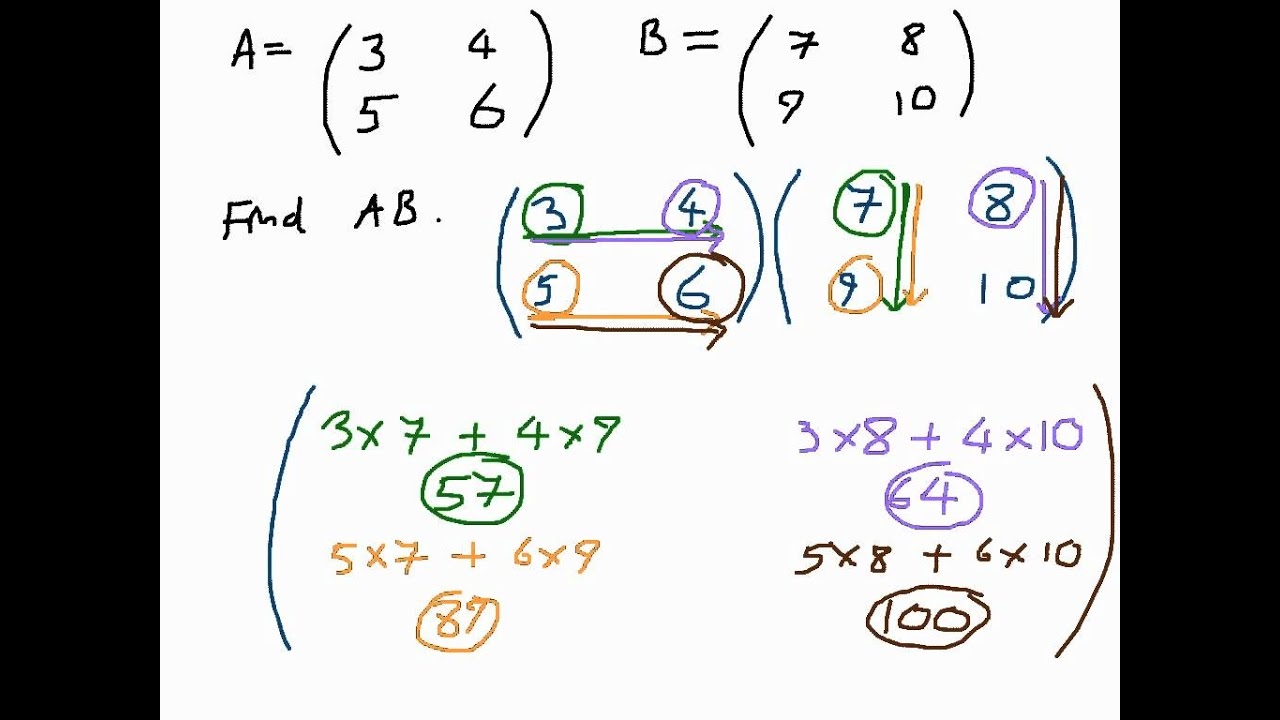
\includegraphics[width=0.8\textwidth]{media/matrix-mult.jpg}}
	\caption{Matrix multiplication as taught in American high school:
		``here's a recipe, trust me bro''. Image from \cite{img:matrixmult}.}
	\label{fig:matmult}
\end{figure}

\subsection{General discussion, back to Napkin levels of abstraction}
Let's go back to modern language,
where we work with finite-dimensional spaces over any field,
and any basis of the spaces (rather than a fixed basis like in the previous section).

Pick a finite-dimensional vector space $V$ with \emph{some} basis $e_1, \dots, e_m$
and a vector space $W$ with basis $w_1, \dots, w_n$.
Suppose I have a map $T \colon V \to W$ and I want to tell you what $T$ is.
It would be awfully inconsiderate of me to try and tell you what $T(v)$
is at every point $v$.
But we saw I only have to tell you what $T(e_1)$, \dots, $T(e_m)$ are,
because from there you can work out
$T(a_1 e_1 + \dots + a_m e_m)$ for yourself:
\[ T(a_1 e_1 + \dots + a_m e_m) = a_1 T(e_1) + \dots + a_m T(e_m). \]
Since the $e_i$ are a basis, that tells you all you need to know about $T$.
\begin{example}
	[Extending linear maps]
	Let $V = \left\{ ax^2+bx+c \mid a,b,c \in \RR \right\}$.
	Then $T(ax^2+bx+c) = aT(x^2) + bT(x) + cT(1)$.
\end{example}

Now I can even be more concrete.
I could tell you what $T(e_1)$ is, but seeing as I have a basis of $W$,
I can actually just tell you what $T(e_1)$ is in terms of this basis.
Specifically, there are unique $a_{11}, a_{21}, \dots, a_{n1} \in k$ such that
\[ T(e_1) = a_{11} w_1 + a_{21} w_2 + \dots + a_{n1} w_n. \]
So rather than telling you the value of $T(e_1)$ in some abstract space $W$,
I could just tell you what $a_{11}, a_{21}, \dots, a_{n1}$ were.
Then I'd repeat this for $T(e_2)$, $T(e_3)$, all the way up to $T(e_m)$,
and that would tell you everything you need to know about $T$.

That's where the matrix $T$ comes from!
It's a concise way of writing down all $mn$ numbers
I need to tell you.

To be explicit, the matrix for $T$ is defined as the array
\begin{align*}
	T &= \underbrace{%
	\begin{bmatrix}
		\mid & \mid & & \mid \\
		T(e_1) & T(e_2) & \dots & T(e_{m}) \\
		\mid & \mid & & \mid \\
	\end{bmatrix}
	}_{\text{$m$ columns}} \Bigg\} \text{$n$ rows} \\
	&=
	\begin{bmatrix}
		a_{11} & a_{12} & \dots & a_{1m} \\
		a_{21} & a_{22} & \dots & a_{2m} \\
		\vdots & \vdots & \ddots & \vdots \\
		a_{n1} & a_{n2} & \dots & a_{nm}
	\end{bmatrix}.
\end{align*}
To drive this point home,
\begin{moral}
	A matrix is the laziest possible way to specify
	a linear map from $V$ to $W$.
\end{moral}

\begin{example}
	[An example of a matrix]
	Here is a concrete example in terms of a basis.
	Let $V = \RR^3$ with basis $e_1$, $e_2$, $e_3$
	and let $W = \RR^2$ with basis $w_1$, $w_2$.
	If I have $T \colon V \to W$
	then uniquely determined by three values, for example:
	\begin{align*}
		T(e_1) &= 4w_1 + 7w_2 \\
		T(e_2) &= 2w_1 + 3w_2 \\
		T(e_3) &= w_1
	\end{align*}
	The columns then correspond to $T(e_1)$, $T(e_2)$, $T(e_3)$:
	\[
		T =
		\begin{bmatrix}
			4 & 2 & 1 \\
			7 & 3 & 0
		\end{bmatrix}
	\]
\end{example}

\begin{example}
	[An example of a matrix after choosing a basis]
	We again let $V = \left\{ ax^2 + bx + c \right\}$
	be the vector space of polynomials of degree at most $2$.
	We fix the basis $1$, $x$, $x^2$ for it.

	Consider the ``evaluation at $3$'' map,
	a map $V \to \RR$.
	We pick $1$ as the basis element of the RHS;
	then we can write it as a $1 \times 3$ matrix
	\[ \begin{bmatrix}
			1 & 3 & 9
		\end{bmatrix} \]
	with the columns corresponding to $T(1)$, $T(x)$, $T(x^2)$.
\end{example}

From here you can actually work out for yourself
what it means to multiply two matrices.
Suppose we have picked a basis for three spaces $U$, $V$, $W$.
Given maps $T \colon U \to V$ and $S \colon V \to W$,
we can consider their composition $S \circ T$, i.e.
\[ U \taking{T} V \taking{S} W. \]
Matrix multiplication is defined exactly so that the matrix $ST$
is the same thing we get from interpreting the composed function $S \circ T$ as a matrix,
as we saw last section.

In particular, since function composition is associative,
it follows that matrix multiplication is as well.

This means you can define concepts like the determinant or the trace of a matrix
both in terms of an ``intrinsic'' map $T \colon V \to W$
and in terms of the entries of the matrix.
Since the map $T$ itself doesn't refer to any basis,
the abstract definition will imply that the numerical definition
doesn't depend on the choice of a basis.

\section{Subspaces and picking convenient bases}
\prototype{Any two linearly independent vectors in $\RR^3$.}
% A submodule is exactly what you think it is.
\begin{definition}
	Let $M$ be a left $R$-module.
	A \vocab{submodule} $N$ of $M$ is a module $N$
	such that every element of $N$ is also an element of $M$.
	If $M$ is a vector space then $N$ is called a \vocab{subspace}.
\end{definition}

\begin{example}[Kernels]
	The \vocab{kernel} of a map $T \colon V \to W$ (written $\ker T$) is
	the set of $v \in V$ such that $T(v) = 0_W$.
	It is a subspace of $V$, since it's closed under addition and scaling (why?).
\end{example}
\begin{example}[Spans]
	Let $V$ be a vector space and $v_1, \dots, v_m$ be any vectors of $V$.
	The \vocab{span} of these vectors is defined as the set
	\[ \left\{ a_1 v_1 + \dots + a_m v_m \mid a_1, \dots, a_m \in k \right\}. \]
	Note that it is a subspace of $V$ as well!
\end{example}
\begin{ques}
	Why is $0_V$ an element of each of the above examples?
	In general, why must any subspace contain $0_V$?
\end{ques}

Subspaces behave nicely with respect to bases.
\begin{theorem}[Basis completion]
	\label{thm:basis_completion}
	Let $V$ be an $n$-dimensional space, and $V'$ a subspace of $V$.
	Then
	\begin{enumerate}[(a)]
		\ii $V'$ is also finite-dimensional.
		\ii If $e_1, \dots, e_m$ is a basis of $V'$, then there exist
		$e_{m+1}, \dots, e_n$ in $V$ such that
		$e_1, \dots, e_n$ is a basis of $V$.
	\end{enumerate}
\end{theorem}
\begin{proof}
	Omitted, since it is intuitive and the proof is not that enlightening.
	(However, we will use this result repeatedly later on,
	so do take the time to internalize it now.)
\end{proof}

A very common use case is picking a convenient basis for a map $T$.
\begin{theorem}[Picking a basis for linear maps]
	\label{thm:linear_map_basis}
	Let $T \colon V \to W$ be a map of finite-dimensional vector spaces,
	with $n = \dim V$, $m = \dim W$.
	Then there exists a basis $v_1, \dots, v_n$ of $V$
	and a basis $w_1, \dots, w_m$ of $W$,
	as well as a nonnegative integer $k$, such that
	\[
		T(v_i) =
		\begin{cases}
			w_i & \text{if $i \le k$} \\
			0_W & \text{if $i > k$}.
		\end{cases}
	\]
	Moreover $\dim \ker T = n-k$ and $\dim T\im(V) = k$.
\end{theorem}
\begin{proof}[Sketch of Proof]
	You might like to try this one yourself before reading on:
	it's a repeated application of \Cref{thm:basis_completion}.

	Let $\ker T$ have dimension $n-k$.
	We can pick $v_{k+1}, \dots, v_{n}$ a basis of $\ker T$.
	Then extend it to a basis $v_1, \dots, v_n$ of $V$.
	The map $T$ is injective over the span of $v_1, \dots, v_k$
	(since only $0_V$ is in the kernel) so its images in $W$ are linearly independent.
	Setting $w_i = T(v_i)$ for each $i$,
	we get some linearly independent set in $W$.
	Then extend it again to a basis of $W$.
\end{proof}

This theorem is super important,
not only because of applications but also
because it will give you the right picture in your head
of how a linear map is supposed to look.
I'll even draw a cartoon of it to make sure you remember:

\begin{center}
\begin{asy}
	unitsize(0.7cm);
	real d = 3;

	filldraw(box( (-3*d/2,3.5), (-d/2,-4.5) ), opacity(0.1)+lightcyan, blue);
	filldraw(box( (d/2,3.5), (3*d/2,-5.5) ), opacity(0.1)+lightred, red);

	label(scale(1.5)*"$V$", (-d,4), blue);
	dot("$e_1$", (-d,3), dir(180), blue);
	dot("$e_2$", (-d,2), dir(180), blue);
	label("$\vdots$", (-d,1), blue);
	dot("$e_k$", (-d,0), dir(180), blue);
	dot("$e_{k+1}$", (-d,-1), dir(180), blue);
	dot("$e_{k+2}$", (-d,-2), dir(180), blue);
	label("$\vdots$", (-d,-3), dir(180), blue);
	dot("$e_n$", (-d,-4), dir(180), blue);

	label(scale(1.5)*"$W$", (d,4), red);
	dot("$f_1$", (d,3), dir(0), red);
	dot("$f_2$", (d,2), dir(0), red);
	label("$\vdots$", (d,1), red);
	dot("$f_k$", (d,0), dir(0), red);
	dot("$f_{k+1}$", (d,-1), dir(0), red);
	dot("$f_{k+2}$", (d,-2), dir(0), red);
	dot("$f_{k+3}$", (d,-3), dir(0), red);
	label("$\vdots$", (d,-4), dir(0), red);
	dot("$f_m$", (d,-5), dir(0), red);

	label("$T$", (0,3), dir(90));
	draw( (-d,3)--(d,3), EndArrow, Margin(3,3) );
	draw( (-d,2)--(d,2), EndArrow, Margin(3,3) );
	draw( (-d,0)--(d,0), EndArrow, Margin(3,3) );
	draw( (-d,-1)--(0,-1), EndArrow, Margin(3,3) );
	draw( (-d,-2)--(0,-2), EndArrow, Margin(3,3) );
	draw( (-d,-4)--(0,-4), EndArrow, Margin(3,3) );
	label("$0$", (0,-1));
	label("$0$", (0,-2));
	label("$0$", (0,-4));

	draw( (5.5,3)--(6,3)--(6,0)--(5.5,0));
	label("$\operatorname{im} T$", (6, 1.5), dir(0));
	draw( (-5.5,-1)--(-6,-1)--(-6,-4)--(-5.5,-4) );
	label("$\ker T$", (-6, -2.5), dir(180));
\end{asy}
\end{center}

In particular, for $T \colon V \to W$,
one can write $V = \ker T \oplus V'$,
so that $T$ annihilates its kernel while sending $V'$
to an isomorphic copy in $W$.

A corollary of this (which you should have expected anyways)
is the so called rank-nullity theorem,
which is the analog of the first isomorphism theorem.
\begin{theorem}
	[Rank-nullity theorem]
	\label{thm:rank_nullity}
	Let $V$ and $W$ be finite-dimensional vector spaces.
	If $T \colon V \to W$, then
	\[ \dim V = \dim \ker T + \dim \img T. \]
\end{theorem}
\begin{ques}
	Conclude the rank-nullity theorem from \Cref{thm:linear_map_basis}.
\end{ques}

\section{A cute application: Lagrange interpolation}
Here's a cute application\footnote{Source: Communicated to me
by Joe Harris at the first Harvard-MIT Undergraduate Math Symposium.}
of linear algebra to a theorem from high school.
\begin{theorem}
	[Lagrange interpolation]
	Let $x_1, \dots, x_{n+1}$ be distinct real numbers
	and $y_1, \dots, y_{n+1}$ any real numbers.
	Then there exists a \emph{unique}
	polynomial $P$ of degree at most $n$
	such that \[ P(x_i) = y_i \] for every $i$.
\end{theorem}
When $n = 1$ for example, this loosely
says there is a unique line joining two points.
\begin{proof}
	The idea is to consider the vector space $V$
	of polynomials with degree at most $n$,
	as well as the vector space $W = \RR^{n+1}$.
	\begin{ques}
		Check that $\dim V = n + 1 = \dim W$.
		This is easiest to do if you pick a basis for $V$,
		but you can then immediately forget about the basis
		once you finish this exercise.
	\end{ques}
	Then consider the linear map $T \colon V \to W$ given by
	\[ P \mapsto \left( P(x_1), \dots, P(x_{n+1}) \right). \]
	This is indeed a linear map because,
	well, $T(P+Q) = T(P)+T(Q)$ and $T(cP) = cT(P)$.
	It also happens to be injective: if $P \in \ker T$,
	then $P(x_1) = \dots = P(x_{n+1}) = 0$,
	but $\deg P \le n$ and so $P$ can only be the zero polynomial.

	So $T$ is an injective map between vector spaces of the same dimension.
	Thus it is actually a bijection, which is exactly what we wanted.
\end{proof}

\section{Pedagogical digression: Arrays of numbers are evil}
\label{sec:basis_evil}

(This whole section is Evan yapping about how to \emph{teach} linear algebra,
so it can be safely skipped.)

As I'll stress repeatedly, a matrix represents a
\emph{linear map between two vector spaces}.
Writing it in the form of an $m \times n$ matrix
is merely a very convenient way to see the map concretely.
But it obfuscates the fact that this map is,
well, a map, not an array of numbers.

If you took high school precalculus, you'll see everything done in terms of matrices.
To any typical high school student, a matrix is an array of numbers.
No one is sure what exactly these numbers represent,
but they're told how to magically multiply these arrays to get more arrays.
They're told that the matrix
\[ \begin{bmatrix}
		1 & 0 & \dots & 0 \\
		0 & 1 & \dots & 0 \\
		\vdots & \vdots & \ddots & \vdots \\
		0 & 0 & \dots & 1 \\
	\end{bmatrix} \]
is an ``identity matrix'', because when you multiply
by another matrix it doesn't change.
Then they're told that the determinant is some magical combination of these
numbers formed by this weird multiplication rule.
No one knows what this determinant does,
other than the fact that $\det(AB) = \det A \det B$,
and something about areas and row operations and Cramer's rule.

Then you go into linear algebra in college, and you do more magic
with these arrays of numbers.
You're told that two matrices $T_1$ and $T_2$ are similar if
\[ T_2 = ST_1S\inv \] for some invertible matrix $S$.
You're told that the trace of a matrix $\Tr T$ is the sum of the diagonal entries.
Somehow this doesn't change if you look at a similar matrix,
but you're not sure why.
Then you define the characteristic polynomial as
\[ p_T(X) = \det (XI - T). \]
Somehow this also doesn't change if you take a similar matrix,
but now you really don't know why.
And then you have the Cayley-Hamilton theorem in all its black magic:
$p_T(T)$ is the zero map.  Out of curiosity you Google the proof,
and you find some ad-hoc procedure which still leaves you
with no idea why it's true.

This is terrible. What's so special about $T_2 = ST_1S\inv$?
Only if you know that the matrices are linear maps does this make sense:
$T_2$ is just $T_1$ rewritten with a different choice of basis.

I really want to push the opposite view.
Linear algebra is the study of \emph{linear maps},
but it is taught as the study of \emph{arrays of numbers},
and no one knows what these numbers mean.
And for a good reason: the numbers are meaningless.
They are a highly convenient way of encoding the matrix,
but they are not the main objects of study,
any more than the dates of events are the main objects of study in history.

The other huge downside is that people get the impression
that the only (real) vector space in existence is $\RR^{\oplus n}$.
As explained in \Cref{rem:vector_spaces_have_essence},
while you \emph{can} work this way if you're a soulless robot,
it's very unnatural for humans to do so.

When I took Math 55a as a freshman at Harvard,
I got the exact opposite treatment:
we did all of linear algebra without writing down a single matrix.
During all this time I was quite confused.
What's wrong with a basis?
I didn't appreciate until later that this approach was the
morally correct way to treat the subject: it made it clear what was happening.

Throughout the Napkin, I've tried to strike a balance between these
two approaches, using matrices when appropriate to illustrate
the maps and to simplify proofs, but ultimately writing
theorems and definitions in their \emph{morally correct} form.
I hope that this has both the advantage of giving the ``right'' definitions
while being concrete enough to be digested.
But I would like to say for the record that,
if I had to pick between the high school approach and the 55a approach,
I would pick 55a in a heartbeat.

\section{A word on general modules}
\prototype{$\ZZ[\sqrt2]$ is a $\ZZ$-module of rank two.}
I focused mostly on vector spaces (aka modules over a field) in this chapter
for simplicity, so I want to make a few remarks about
modules over a general commutative ring $R$ before concluding.

Firstly, recall that for general modules,
we say ``generating set'' instead of ``spanning set''.
Shrug.

The main issue with rings is that our key theorem \Cref{thm:vector_best}
fails in spectacular ways.
For example, consider $\ZZ$ as a $\ZZ$-module over itself.
Then $\{2\}$ is linearly independent, but it cannot be extended to a basis.
Similarly, $\{2,3\}$ is spanning, but one cannot cut it down to a basis.
You can see why defining dimension is going to be difficult.

Nonetheless, there are still analogs of some of the definitions above.
\begin{definition}
	An $R$-module $M$ is called \vocab{finitely generated} if it has a finite generating set.
\end{definition}
\begin{definition}
	An $R$-module $M$ is called \vocab{free} if it has a basis.
	As said before, the analogue of the dimension theorem holds,
	and we use the word \vocab{rank} to denote the size of the basis.
	As before, there's an isomorphism $M \cong R^{\oplus n}$ where $n$ is the rank.
\end{definition}
\begin{example}[An example of a $\ZZ$-module]
	The $\ZZ$-module
	\[ \ZZ[\sqrt2] = \left\{ a + b\sqrt 2 \mid a,b \in \ZZ \right\} \]
	has a basis $\{1, \sqrt 2\}$, so we say it is
	a free $\ZZ$-module of rank $2$.
\end{example}

\begin{abuse}
	[Notation for groups]
	Recall that an abelian group
	can be viewed a $\ZZ$-module (and in fact vice-versa!),
	so we can (and will) apply these words to abelian groups.
	We'll use the notation $G \oplus H$ for two abelian groups $G$ and $H$
	for their Cartesian product, emphasizing the fact that $G$ and $H$ are abelian.
	This will happen when we study algebraic number theory and homology groups.
\end{abuse}

\section{\problemhead}
General hint:
\Cref{thm:linear_map_basis} will be your best friend
for many of these problems.

\begin{dproblem}
	Let $V$ and $W$ be finite-dimensional vector spaces
	with nonzero dimension, and consider linear maps $T \colon V \to W$.
	Complete the following table by writing
	``sometimes'', ``always'', or ``never'' for each entry.
	\begin{center}
	\begin{tabular}[h]{c|ccc}
		& $T$ injective & $T$ surjective & $T$ isomorphism \\ \hline
		If $\dim V > \dim W$\dots \\
		If $\dim V = \dim W$\dots \\
		If $\dim V < \dim W$\dots \\
	\end{tabular}
	\end{center}
	\begin{hint}
		Use the rank-nullity theorem.
		Also consider the zero map.
	\end{hint}
	\begin{sol}
		\begin{center}
		\begin{tabular}[h]{c|ccc}
		& $T$ injective & $T$ surjective & $T$ isomorphism \\ \hline
		If $\dim V > \dim W$\dots & never & sometimes & never\\
		If $\dim V = \dim W$\dots & sometimes & sometimes & sometimes \\
		If $\dim V < \dim W$\dots & sometimes & never & never \\
		\end{tabular}
		\end{center}
		Each ``never'' is by the rank-nullity theorem.
		Each counterexample is obtained by the zero map
		sending every element of $V$ to zero;
		this map is certainly neither injective or surjective.
	\end{sol}
\end{dproblem}

\begin{dproblem}
	[Equal dimension vector spaces are usually isomorphisms]
	\label{prob:equal_dimension}
	Let $V$ and $W$ be finite-dimensional vector
	spaces with $\dim V = \dim W$.
	Prove that for a map $T \colon V \to W$,
	the following are equivalent:
	\begin{itemize}
		\ii $T$ is injective,
		\ii $T$ is surjective,
		\ii $T$ is bijective.
	\end{itemize}
	\begin{sol}
		It essentially follows by \Cref{thm:linear_map_basis}.
	\end{sol}
\end{dproblem}

\begin{problem}
	Let's say a \emph{magic square} is a $3 \times 3$ matrix of real numbers
	where the sum of all diagonals, columns, and rows is equal, such as
	$\left[ \begin{smallmatrix}
		8 & 1 & 6 \\
		3 & 5 & 7 \\
		4 & 9 & 2
	\end{smallmatrix} \right]$.
	Find the dimension of the set of magic squares, as a real vector space under addition.
\end{problem}

\begin{problem}
	[Multiplication by $\sqrt5$]
	Let $V = \QQ[\sqrt5] = \left\{ a + b \sqrt 5 \right\}$
	be a two-dimensional $\QQ$-vector space,
	and fix the basis $\{1, \sqrt 5\}$ for it.
	Write down the $2 \times 2$ matrix with rational coefficients
	that corresponds to multiplication by $\sqrt 5$.
	\begin{hint}
		$a + b \sqrt 5 \mapsto \sqrt 5 a + 5b$.
	\end{hint}
	\begin{sol}
		Since $1 \mapsto \sqrt5$ and $\sqrt5 \mapsto 5$,
		the matrix is
		$\begin{bmatrix}
			0 & 5 \\
			1 & 0
		\end{bmatrix}$.
	\end{sol}
\end{problem}

\begin{problem}
	[Multivariable Lagrange interpolation]
	Let $S \subset {\mathbb Z}^2$ be a set of $n$ lattice points.
	Prove that there exists a nonzero two-variable polynomial $p$
	with real coefficients, of degree at most $\sqrt{2n}$,
	such that $p(x,y) = 0$ for every $(x,y) \in S$.
\end{problem}

\begin{problem}
	[Putnam 2003]
	Do there exist polynomials $a(x)$, $b(x)$, $c(y)$, $d(y)$ such that
	\[ 1 + xy + (xy)^2 = a(x)c(y) + b(x)d(y) \]
	holds identically?
	\begin{hint}
		Plug in $y = -1, 0, 1$. Use dimensions of $\RR[x]$.
	\end{hint}
\end{problem}

\begin{problem}[TSTST 2014]
	\gim
	Let $P(x)$ and $Q(x)$ be arbitrary polynomials with real coefficients,
	and let $d$ be the degree of $P(x)$.
	Assume that $P(x)$ is not the zero polynomial.
	Prove that there exist polynomials $A(x)$ and $B(x)$ such that
	\begin{enumerate}[(i)]
		\ii Both $A$ and $B$ have degree at most $d/2$,
		\ii At most one of $A$ and $B$ is the zero polynomial,
		\ii $P$ divides $A+Q \cdot B$.
	\end{enumerate}
	\begin{hint}
		Interpret as $V \oplus V \to W$ for suitable $V$, $W$.
	\end{hint}
	\begin{sol}
		Let $V$ be the space of real polynomials with degree at most $d/2$
		(which has dimension $1 + \left\lfloor d/2 \right\rfloor$),
		and $W$ be the space of real polynomials modulo $P$ (which has dimension $d$).
		Then $\dim (V \oplus V) > \dim W$.
		So the linear map $V \oplus V \to W$ by $(A,B) \mapsto A + Q \cdot B$
		has a kernel of positive dimension
		(by rank-nullity, for example).
	\end{sol}
\end{problem}

\begin{sproblem}
	[Idempotents are projection maps]
	\label{prob:idempotent}
	Let $P \colon V \to V$ be a linear map,
	where $V$ is a vector space
	(not necessarily finite-dimensional).
	Suppose $P$ is \vocab{idempotent},
	meaning $P(P(v)) = P(v)$ for each $v \in V$,
	or equivalently $P$ is the identity on its image.
	Prove that \[ V = \ker P \oplus \img P. \]
	Thus we can think of $P$ as \emph{projection}
	onto the subspace $\img P$.
\end{sproblem}

\begin{sproblem}
	\label{prob:endomorphism_eventual_lemma}
	\gim
	Let $V$ be a finite dimensional vector space.
	Let $T \colon V \to V$ be a linear map,
	and let $T^n \colon V \to V$ denote $T$ applied $n$ times.
	Prove that there exists an integer $N$ such that
	\[ V = \ker T^N \oplus \img T^N. \]
	\begin{hint}
		Use the fact that the infinite chain of subspaces
		\[ \ker T \subseteq \ker T^2 \subseteq \ker T^3 \subseteq \dots \]
		and the similar chain for $\img T$ must eventually stabilize
		(for dimension reasons).
	\end{hint}
	\begin{sol}
		Consider
		\[
			\{0\} \subsetneq \ker S \subseteq \ker S^2 \subseteq \ker S^3 \subseteq \dots
			\text{  and  }
			V \supsetneq \img S \supseteq \img S^2 \supseteq \img S^3 \supseteq \dots.
		\]
		For dimension reasons, these subspaces must eventually stabilize:
		for some large integer $N$,
		$\ker T^N = \ker T^{N+1} = \dots$
		and $\img T^N = \img T^{N+1} = \img T^{N+2} = \dots$.
		When this happens, $\ker T^N \bigcap \img T^N = \{0\}$,
		since $T^N$ is an automorphism of $\img T^N$.
		On the other hand, by Rank-Nullity we also have
		$\dim \ker T^N + \dim \img T^n = \dim V$.
		Thus for dimension reasons, $V = \ker T^N \oplus \img T^N$.
	\end{sol}
\end{sproblem}

%Now consider the sequences

\chapter{Eigen-things}
This chapter will develop the theory of eigenvalues and eigenvectors,
the so-called ``Jordan canonical form''.
(Later on we will use it to
define the characteristic polynomial.)

\section{Why you should care}
We know that a square matrix $T$ is really just
a linear map from $V$ to $V$.
What's the simplest type of linear map?
It would just be multiplication by some scalar $\lambda$,
which would have associated matrix (in any basis!)
\[
	T =
	\begin{bmatrix}
		\lambda & 0 & \dots & 0 \\
		0 & \lambda & \dots & 0 \\
		\vdots & \vdots & \ddots & \vdots \\
		0 & 0 & \dots & \lambda
	\end{bmatrix}.
\]
That's perhaps \emph{too} simple, though.
If we had a fixed basis $e_1, \dots, e_n$
then another very ``simple'' operation
would just be scaling each basis element $e_i$ by $\lambda_i$,
i.e.\ a \vocab{diagonal matrix} of the form
\[
	T = \begin{bmatrix}
		\lambda_1 & 0 & \dots & 0 \\
		0 & \lambda_2 & \dots & 0 \\
		\vdots & \vdots & \ddots & \vdots \\
		0 & 0 & \dots & \lambda_n
	\end{bmatrix}.
\]
These maps are more general.
Indeed, you can, for example, compute $T^{100}$ in a heartbeat:
the map sends $e_i \to \lambda_i^{100} e_i$.
(Try doing that with an arbitrary $n \times n$ matrix.)

Of course, most linear maps are probably not that nice.
Or are they?
\begin{example}
	[Getting lucky]
	Let $V$ be some two-dimensional vector space
	with $e_1$ and $e_2$ as basis elements.
	Let's consider a map $T \colon V \to V$
	by $e_1 \mapsto 2e_1$ and $e_2 \mapsto e_1+3e_2$,
	which you can even write concretely as
	\[ T = \begin{bmatrix}
		2 & 1 \\
		0 & 3
	\end{bmatrix} \quad\text{in basis $e_1$, $e_2$}. \]
	This doesn't look anywhere as nice until we realize we can rewrite it as
	\begin{align*}
		e_1 &\mapsto 2e_1 \\
		e_1+e_2 &\mapsto 3(e_1+e_2).
	\end{align*}
	So suppose we change to the basis $e_1$ and $e_1 + e_2$.
	Thus in the new basis,
	\[ T = \begin{bmatrix}
		2 & 0 \\
		0 & 3
	\end{bmatrix} \quad\text{in basis $e_1$, $e_1+e_2$}. \]
	So our completely random-looking map,
	under a suitable change of basis,
	looks like the very nice maps we described before!
\end{example}
In this chapter, we will be \emph{making} our luck,
and we will see that our better understanding of matrices
gives us the right way to think about this.

\section{Warning on assumptions}
Most theorems in this chapter only work for
\begin{itemize}
	\ii finite-dimensional vector spaces $V$,
	\ii over a field $k$ which is \emph{algebraically closed}.
\end{itemize}
On the other hand, the definitions work fine without
these assumptions.

\section{Eigenvectors and eigenvalues}
Let $k$ be a field and $V$ a vector space over it.
In the above example, we saw that there were two very nice
vectors, $e_1$ and $e_1+e_2$, for which $V$ did something very simple.
Naturally, these vectors have a name.
\begin{definition}
	Let $T \colon V \to V$ and $v \in V$ a \emph{nonzero} vector.
	We say that $v$ is an \vocab{eigenvector} if $T(v) = \lambda v$
	for some $\lambda \in k$ (possibly zero, but remember $v \neq 0$).
	The value $\lambda$ is called an \vocab{eigenvalue} of $T$.

	We will sometimes abbreviate
	``$v$ is an eigenvector with eigenvalue $\lambda$''
	to just ``$v$ is a $\lambda$-eigenvector''.
\end{definition}
Of course, no mention to a basis anywhere.

\begin{example}
	[An example of an eigenvector and eigenvalue]
	Consider the example earlier with
	$T = \begin{bmatrix} 2 & 1 \\ 0 & 3 \end{bmatrix}$.
	\begin{enumerate}[(a)]
		\ii Note that $e_1$ and $e_1 + e_2$ are
		$2$-eigenvectors and $3$-eigenvectors.
		\ii Of course, $5e_1$ is also an $2$-eigenvector.
		\ii And, $7e_1 + 7e_2$ is also a $3$-eigenvector.
	\end{enumerate}
\end{example}
So you can quickly see the following observation.
\begin{ques}
	Show that the $\lambda$-eigenvectors, together with $\{0\}$
	form a subspace.
\end{ques}
\begin{definition}
	For any $\lambda$, we define the $\lambda$-\vocab{eigenspace}
	as the set of $\lambda$-eigenvectors together with $0$.
\end{definition}
This lets us state succinctly that
``$2$ is an eigenvalue of $T$
with one-dimensional eigenspace spanned by $e_1$''.

Unfortunately, it's not exactly true that eigenvalues always exist.
\begin{example}[Eigenvalues need not exist]
	Let $V = \RR^2$ and let $T$ be the map
	which rotates a vector by $90\dg$
	around the origin.
	Then $T(v)$ is not a multiple of $v$ for any $v \in V$,
	other than the trivial $v=0$.
\end{example}

However, it is true if we replace $k$ with an
algebraically closed field\footnote{A field is \vocab{algebraically closed}
	if all its polynomials have roots,
	the archetypal example being $\CC$.}.
\begin{theorem}[Eigenvalues always exist over algebraically closed fields]
	Suppose $k$ is an \emph{algebraically closed} field.
	Let $V$ be a finite dimensional $k$-vector space.
	Then if $T \colon V \to V$ is a linear map,
	there exists an eigenvalue $\lambda \in k$.
\end{theorem}
\begin{proof}
	(From \cite{ref:axler})
	The idea behind this proof is to consider ``polynomials'' in $T$.
	For example, $2T^2-4T+5$ would be shorthand for $2T(T(v)) - 4T(v) + 5v$.
	In this way we can consider ``polynomials'' $P(T)$;
	this lets us tie in the ``algebraically closed'' condition.
	These polynomials behave nicely:
	\begin{ques}
		Show that $P(T)+Q(T) = (P+Q)(T)$ and $P(T) \circ Q(T) = (P \cdot Q)(T)$.
	\end{ques}

	Let $n = \dim V < \infty$ and fix any nonzero vector $v \in V$,
	and consider vectors $v$, $T(v)$, \dots, $T^n (v)$.
	There are $n+1$ of them,
	so they can't be linearly independent for dimension reasons;
	thus there is a nonzero polynomial $P$ such that $P(T)$
	is zero when applied to $v$.
	WLOG suppose $P$ is a monic polynomial,
	and thus $P(z) = (z-r_1)\dots(z-r_m)$ say.
	Then we get
	\[ 0 = (T - r_1 \id) \circ (T - r_2 \id) \circ \dots
		\circ (T - r_m \id)(v) \]
	(where $\id$ is the identity matrix).  This means at least one of
	$T - r_i \id$ is not injective, i.e.\ has a nontrivial kernel,
	which is the same as an eigenvector.
\end{proof}
So in general we like to consider algebraically closed fields.
This is not a big loss:
any real matrix can be interpreted as a complex matrix
whose entries just happen to be real, for example.

\section{The Jordan form}
So that you know exactly where I'm going,
here's the main theorem.
\begin{definition}
	A \vocab{Jordan block} is an $n \times n$ matrix of the following shape:
	\[
		\begin{bmatrix}
			\lambda & 1 & 0 & 0 & \dots & 0 & 0 \\
			0 & \lambda & 1 & 0 & \dots & 0 & 0 \\
			0 & 0 & \lambda & 1 & \dots & 0 & 0 \\
			0 & 0 & 0 & \lambda & \dots & 0 & 0 \\
			\vdots & \vdots & \vdots & \vdots & \ddots & \vdots & \vdots \\
			0 & 0 & 0 & 0 & \dots & \lambda & 1 \\
			0 & 0 & 0 & 0 & \dots & 0 & \lambda
		\end{bmatrix}.
	\]
	In other words, it has $\lambda$ on the diagonal,
	and $1$ above it.
	We allow $n = 1$,
	so $\begin{bmatrix} \lambda \end{bmatrix}$ is a Jordan block.
\end{definition}

\begin{theorem}
	[Jordan canonical form]
	Let $T \colon V \to V$ be a linear map
	of finite-dimensional vector spaces
	over an algebraically closed field $k$.
	Then we can choose a basis of $V$
	such that the matrix $T$ is ``block-diagonal''
	with each block being a Jordan block.

	Such a matrix is said to be in \vocab{Jordan form}.
	This form is unique up to rearranging the order of the blocks.
\end{theorem}
As an example, this means the matrix should look something like:
\[
	\begin{bmatrix}
		\lambda_1 & 1 \\
		0 & \lambda_1 \\
		&& \lambda_2 \\
		&&& \lambda_3 & 1 & 0 \\
		&&& 0 & \lambda_3 & 1 \\
		&&& 0 & 0 & \lambda_3 \\
		&&&&&& \ddots \\
		&&&&&&& \lambda_m & 1 \\
		&&&&&&& 0 & \lambda_m
	\end{bmatrix}
\]
\begin{ques}
	Check that diagonal matrices are the special case
	when each block is $1 \times 1$.
\end{ques}

What does this mean?
Basically, it means \emph{our dream is almost true}.
What happens is that $V$ can get broken down as a direct sum
\[ V = J_1 \oplus J_2 \oplus \dots \oplus J_m \]
and $T$ acts on each of these subspaces independently.
These subspaces correspond to the blocks in the matrix above.
In the simplest case, $\dim J_i = 1$,
so $J_i$ has a basis element $e$
for which $T(e) = \lambda_i e$;
in other words, we just have a simple eigenvalue.
But on occasion, the situation is not quite so simple,
and we have a block of size greater than $1$;
this leads to $1$'s just above the diagonals.

I'll explain later how to interpret the $1$'s,
when I make up the word \emph{descending staircase}.
For now, you should note that even if $\dim J_i \ge 2$,
we still have a basis element
which is an eigenvector with eigenvalue $\lambda_i$.

\begin{example}
	[A concrete example of Jordan form]
	Let $T \colon k^6 \to k^6$ and suppose $T$ is given by the matrix
	\[
		T = \begin{bmatrix}
			5 & 0 & 0 & 0 & 0 & 0 \\
			0 & 2 & 1 & 0 & 0 & 0 \\
			0 & 0 & 2 & 0 & 0 & 0 \\
			0 & 0 & 0 & 7 & 0 & 0 \\
			0 & 0 & 0 & 0 & 3 & 0 \\
			0 & 0 & 0 & 0 & 0 & 3 \\
		\end{bmatrix}.
	\]
	Reading the matrix, we can compute all the eigenvectors and eigenvalues:
	for any constants $a, b \in k$ we have
	\begin{align*}
		T(a \cdot e_1) &= 5a \cdot e_1 \\
		T(a \cdot e_2) &= 2a \cdot e_2 \\
		T(a \cdot e_4) &= 7a \cdot e_4 \\
		T(a \cdot e_5 + b \cdot e_6) &= 3\left[ a \cdot e_5 + b \cdot e_6 \right].
	\end{align*}
	The element $e_3$ on the other hand,
	is not an eigenvector since $T(e_3) = e_2 + 2e_3$.
\end{example}

%Here's the idea behind the proof.
%We would like to be able to break down $V$ directly into components as above,
%but some of the $\lambda_i$'s from the different Jordan blocks could coincide,
%and this turns out to give a technical difficulty for detecting them.
%So instead, we're going to break down $V$ first into subspaces
%based on the values of $\lambda$'s;
%these are called the \emph{generalized eigenspaces}.
%In other words, the generalized eigenspace of a given $\lambda$
%is just all the Jordan blocks which have eigenvalue $\lambda$.
%Only after that will we break the generalized eigenspace
%into the individual Jordan blocks.
%
%The sections below record this proof in the other order:
%the next part deals with breaking generalized
%eigenspaces into Jordan blocks,
%and the part after that is the one where we break down $V$ into
%generalized eigenspaces.

\section{Nilpotent maps}
Bear with me for a moment.  First, define:
\begin{definition}
	A map $T \colon V \to V$ is \vocab{nilpotent} if $T^m$ is the zero map for some integer $m$.
	(Here $T^m$ means ``$T$ applied $m$ times''.)
\end{definition}
What's an example of a nilpotent map?
\begin{example}
	[The ``descending staircase'']
        Let $V = k^{\oplus 3}$ have basis $e_1$, $e_2$, $e_3$.
	Then the map $T$ which sends
	\[ e_3 \mapsto e_2 \mapsto e_1 \mapsto 0 \]
	is nilpotent, since $T(e_1) = T^2(e_2) = T^3(e_3) = 0$,
	and hence $T^3(v) = 0$ for all $v \in V$.
\end{example}
The $3 \times 3$ descending staircase has matrix representation
\[ T = \begin{bmatrix}
		0 & 1 & 0 \\
		0 & 0 & 1 \\
		0 & 0 & 0
	\end{bmatrix}. \]
You'll notice this is a Jordan block.
\begin{exercise}
	Show that the descending staircase above
	has $0$ as its only eigenvalue.
\end{exercise}

That's a pretty nice example.
As another example, we can have multiple such staircases.
\begin{example}
	[Double staircase]
	Let $V = k^{\oplus 5}$ have basis $e_1$, $e_2$, $e_3$, $e_4$, $e_5$.
	Then the map
	\[ e_3 \mapsto e_2 \mapsto e_1 \mapsto 0 \text{ and }
		e_5 \mapsto e_4 \mapsto 0 \]
	is nilpotent.
\end{example}
Picture, with some zeros omitted for emphasis:
\[ T = \begin{bmatrix}
		0 & 1 & 0 &   &   \\
		0 & 0 & 1 &   &   \\
		0 & 0 & 0 &   &   \\
		  &   &   & 0 & 1 \\
		  &   &   & 0 & 0 \\
	\end{bmatrix}
\]
You can see this isn't really that different
from the previous example;
it's just the same idea repeated multiple times.
And in fact we now claim that \emph{all}
nilpotent maps have essentially that form.
\begin{theorem}
	[Nilpotent Jordan]
	Let $V$ be a finite-dimensional vector space
	over an algebraically closed field $k$.
	Let $T \colon V \to V$ be a nilpotent map.
	Then we can write $V = \bigoplus_{i=1}^m V_i$
	where each $V_i$ has a basis of the form
	$v_i$, $T(v_i)$, \dots, $T^{\dim V_i - 1}(v_i)$
	for some $v_i \in V_i$.
\end{theorem}
Hence:
\begin{moral}
	Every nilpotent map can be viewed as independent staircases.
\end{moral}
Each chain $v_i$, $T(v_i)$, $T(T(v_i))$, \dots is just one staircase.
The proof is given later, but first let me point out where this is going.

Here's the punch line.
Let's take the double staircase again.
Expressing it as a matrix gives, say
\[
	S = \begin{bmatrix}
		0 & 1 & 0 &   &   \\
		0 & 0 & 1 &   &   \\
		0 & 0 & 0 &   &   \\
		  &   &   & 0 & 1 \\
		  &   &   & 0 & 0
	\end{bmatrix}.
\]
Then we can compute
\[
	S + \lambda \id = \begin{bmatrix}
		\lambda & 1 & 0 &   &   \\
		0 & \lambda & 1 &   &   \\
		0 & 0 & \lambda &   &   \\
		  &   &   & \lambda & 1 \\
		  &   &   & 0 & \lambda
	\end{bmatrix}.
\]
It's a bunch of $\lambda$ Jordan blocks!
This gives us a plan to proceed: we need to break $V$ into
a bunch of subspaces such that $T - \lambda \id$ is nilpotent over each subspace.
Then Nilpotent Jordan will finish the job.

\section{Reducing to the nilpotent case}
\begin{definition}
	Let $T \colon V \to V$. A subspace $W \subseteq V$
	is called $T$-\vocab{invariant}
	if $T(w) \in W$ for any $w \in W$.
	In this way, $T$ can be thought of as a map $W \to W$.
\end{definition}
In this way, the Jordan form is a decomposition of $V$ into invariant subspaces.

Now I'm going to be cheap, and define:
\begin{definition}
	A map $T \colon V \to V$ is called \vocab{indecomposable}
	if it's impossible to write $V = W_1 \oplus W_2$
	where both $W_1$ and $W_2$ are nontrivial $T$-invariant spaces.
\end{definition}
Picture of a \emph{decomposable} map:
\[
	\begin{bmatrix}
		\multicolumn{2}{c|}{\multirow{2}{*}{$W_1$}} & 0 & 0 & 0  \\
		\multicolumn{2}{c|}{} & 0 & 0 & 0 \\ \hline
		0 & 0 & \multicolumn{3}{|c}{\multirow{3}{*}{$W_2$}} \\
		0 & 0 & \multicolumn{3}{|c}{} \\
		0 & 0 & \multicolumn{3}{|c}{}
	\end{bmatrix}
\]
As you might expect, we can break a space apart into ``indecomposable'' parts.
\begin{proposition}
	[Invariant subspace decomposition]
	Let $V$ be a finite-dimensional vector space.
	Given any map $T \colon V \to V$, we can write
	\[ V = V_1 \oplus V_2 \oplus \dots \oplus V_m \]
	where each $V_i$ is $T$-invariant,
	and for any $i$ the map $T \colon V_i \to V_i$ is indecomposable.
\end{proposition}
\begin{proof}
	Same as the proof that every integer is the product of primes.
	If $V$ is not decomposable, we are done.
	Otherwise, by definition write $V = W_1 \oplus W_2$
	and then repeat on each of $W_1$ and $W_2$.
\end{proof}

Incredibly, with just that we're almost done!
Consider a decomposition as above,
so that $T \colon V_1 \to V_1$ is an indecomposable map.
Then $T$ has an eigenvalue $\lambda_1$, so let $S = T - \lambda_1 \id$; hence $\ker S \neq \{0\}$.
\begin{ques}
	Show that $V_1$ is also $S$-invariant, so we can consider $S \colon V_1 \to V_1$.
\end{ques}
By \Cref{prob:endomorphism_eventual_lemma}, we have
\[ V_1 = \ker S^N \oplus \img S^N \]
for some $N$.
But we assumed $T$ was indecomposable,
so this can only happen if $\img S^N = \{0\}$ and $\ker S^N = V_1$
(since $\ker S^N$ contains our eigenvector).
Hence $S$ is nilpotent, so it's a collection of staircases.
In fact, since $T$ is indecomposable, there is only one staircase.
Hence $V_1$ is a Jordan block, as desired.

\section{(Optional) Proof of nilpotent Jordan}
The proof is just induction on $\dim V$.
Assume $\dim V \ge 1$, and let $W = T\im(V)$ be the image of $V$.
Since $T$ is nilpotent, we must have $W \subsetneq V$.
Moreover, if $W = \{0\}$ (i.e.\ $T$ is the zero map) then we're already done.
So assume $\{0\} \subsetneq W \subsetneq V$.

By the inductive hypothesis, we can select a good basis of $W$:
\begin{align*}
	\mathcal B' =
	\Big\{ & T(v_1), T(T(v_1)), T(T(T(v_1))), \dots \\
	& T(v_2), T(T(v_2)), T(T(T(v_2))), \dots \\
	& \dots, \\
	& T(v_\ell), T(T(v_\ell)), T(T(T(v_\ell))), \dots \Big\}
\end{align*}
for some $T(v_i) \in W$ (here we have taken advantage of the fact that each element of $W$ is itself of the form $T(v)$ for some $v$).

Also, note that there are exactly $\ell$ elements of $\mathcal B'$ which are in $\ker T$
(namely the last element of each of the $\ell$ staircases).
We can thus complete it to a basis $v_{\ell+1}, \dots, v_m$ (where $m = \dim \ker T$).
(In other words, the last element of each staircase plus the $m-\ell$ new ones are a basis for $\ker T$.)

Now consider
\begin{align*}
	\mathcal B =
	\Big\{ & v_1, T(v_1), T(T(v_1)), T(T(T(v_1))), \dots \\
	& v_2, T(v_2), T(T(v_2)), T(T(T(v_2))), \dots \\
	& \dots, \\
	& v_\ell, T(v_\ell), T(T(v_\ell)), T(T(T(v_\ell))), \dots \\
	& v_{\ell+1}, v_{\ell+2}, \dots, v_m \Big\}.
\end{align*}
\begin{ques}
Check that there are exactly $\ell + \dim W + (\dim \ker T - \ell) = \dim V$ elements.
\end{ques}
\begin{exercise}
	Show that all the elements are linearly independent.
	(Assume for contradiction there is some linear dependence,
	then take $T$ of both sides.)
\end{exercise}
Hence $\mathcal B$ is a basis of the desired form.

\section{Algebraic and geometric multiplicity}
\prototype{The matrix $T$ below.}
This is some convenient notation:
let's consider the matrix in Jordan form
\[
	T =
	\begin{bmatrix}
		7 & 1 \\
		0 & 7 \\
		& & 9 \\
		& & & 7 & 1 & 0 \\
		& & & 0 & 7 & 1 \\
		& & & 0 & 0 & 7
	\end{bmatrix}.
\]
We focus on the eigenvalue $7$,
which appears multiple times, so it is certainly ``repeated''.
However, there are two different senses in which you could say it is repeated.
\begin{itemize}
	\ii \emph{Algebraic}: You could say it is repeated five times,
	because it appears five times on the diagonal.
	\ii \emph{Geometric}: You could say it really only appears two times:
	because there are only two eigen\emph{vectors}
	with eigenvalue $7$, namely $e_1$ and $e_4$.

	Indeed, the vector $e_2$ for example has $T(e_2) = 7e_2 + e_1$,
	so it's not really an eigenvector!
	If you apply $T - 7\id$ to $e_2$ twice though,
	you do get zero.
\end{itemize}
\begin{ques}
	In this example,
	how many times do you need to apply $T - 7\id$ to $e_6$ to get zero?
\end{ques}
Both these notions are valid,
so we will name both.
To preserve generality,
we first state the ``intrinsic'' definition.
\begin{definition}
	Let $T \colon V \to V$ be a linear map and $\lambda$ a scalar.
	\begin{itemize}
		\ii The \vocab{geometric multiplicity}
		of $\lambda$ is the dimension $\dim V_\lambda$
		of the $\lambda$-eigenspace.

		\ii Define the \vocab{generalized eigenspace}
		$V^\lambda$ to be the subspace of $V$
		for which $(T-\lambda \id)^n(v) = 0$ for some $n \ge 1$.
		The \vocab{algebraic multiplicity} of $\lambda$ is the
		dimension $\dim V^\lambda$.
	\end{itemize}
	(Silly edge case: we allow ``multiplicity zero''
	if $\lambda$ is not an eigenvalue at all.)
\end{definition}
However in practice you should just count the Jordan blocks.
\begin{example}
	[An example of eigenspaces via Jordan form]
	Retain the matrix $T$ mentioned earlier and let $\lambda = 7$.
	\begin{itemize}
		\ii The eigenspace $V_\lambda$ has basis $e_1$ and $e_4$,
		so the geometric multiplicity is $2$.
		\ii The generalized eigenspace $V^\lambda$ has basis $e_1$, $e_2$,
		$e_4$, $e_5$, $e_6$ so the algebraic multiplicity is $5$.
	\end{itemize}
\end{example}

To be completely explicit, here is how you think of these in practice:
\begin{proposition}
	[Geometric and algebraic multiplicity vs Jordan blocks]
	Assume $T \colon V \to V$ is a linear map
	of finite-dimensional vector spaces,
	written in Jordan form.
	Let $\lambda$ be a scalar.
	Then
	\begin{itemize}
		\ii The geometric multiplicity of $\lambda$ is the number
		of Jordan blocks with eigenvalue $\lambda$;
		the eigenspace has one basis element per Jordan block.

		\ii The algebraic multiplicity of $\lambda$ is the
		sum of the dimensions of the Jordan blocks
		with eigenvalue $\lambda$;
		the eigenspace is the direct sum of the subspaces
		corresponding to those blocks.
	\end{itemize}
\end{proposition}

\begin{ques}
	Show that the geometric multiplicity
	is always less than or equal to the algebraic multiplicity.
\end{ques}

This actually gives us a tentative definition:
\begin{itemize}
	\ii The trace is the sum of the eigenvalues,
	counted with algebraic multiplicity.
	\ii The determinant is the product of the eigenvalues,
	counted with algebraic multiplicity.
\end{itemize}
This definition is okay,
but it has the disadvantage of requiring the ground
field to be algebraically closed.
It is also not the definition that is easiest
to work with computationally.
The next two chapters will give us a better definition.

\section\problemhead

\begin{problem}
	[Sum of algebraic multiplicities]
	Given a $2018$-dimensional complex vector space $V$
	and a map $T \colon V \to V$,
	what is the sum of the algebraic multiplicities
	of all eigenvalues of $T$?
	\begin{sol}
		It's just $\dim V = 2018$.
		After all, you are adding the dimensions of the Jordan blocks\dots
	\end{sol}
\end{problem}

\begin{problem}
	[The word ``diagonalizable'']
	A linear map $T \colon V \to V$ (where $\dim V$ is finite)
	is said to be \vocab{diagonalizable}
	if it has a basis $e_1$, \dots, $e_n$
	such that each $e_i$ is an eigenvector.
	\begin{enumerate}[(a)]
		\ii Explain the name ``diagonalizable''.
		\ii Suppose we are working over an algebraically closed field.
		Then show that $T$ is diagonalizable if and only if
		for any $\lambda$, the geometric multiplicity of $\lambda$
		equals the algebraic multiplicity of $\lambda$.
	\end{enumerate}
	\begin{sol}
		(a): if you express $T$ as a matrix in such a basis,
		one gets a diagonal matrix.
		(b): this is just saying each Jordan block has dimension $1$,
		which is what we wanted.
		(We are implicitly using uniqueness of Jordan form here.)
	\end{sol}
\end{problem}

\begin{problem}
	[Switcharoo]
	Let $V$ be the $\CC$-vector space
	with basis $e_1$ and $e_2$.
	The map $T \colon V \to V$ sends $T(e_1) = e_2$ and $T(e_2) = e_1$.
	Determine the eigenspaces of $T$.
	\begin{sol}
		The $+1$ eigenspace is spanned by $e_1+e_2$.
		The $-1$ eigenspace is spanned by $e_1-e_2$.
	\end{sol}
\end{problem}

\begin{problem}
	Suppose $T \colon \CC^{\oplus 2} \to \CC^{\oplus 2}$
	is a linear map of $\CC$-vector spaces such that $T^{2011} = \id$.
	Must $T$ be diagonalizable?
	\begin{hint}
		The answer is yes.
		In fact, the result is true if $\CC^{\oplus 2}$ is any finite-dimensional
		$\CC$-vector space.
	\end{hint}
\end{problem}

\begin{problem}
	[Writing a polynomial backwards]
	Define the complex vector space $V$
	of polynomials with degree at most $2$,
	say $V = \left\{ ax^2 + bx + c \mid a,b,c \in \CC \right\}$.
	Define $T \colon V \to V$ by
	\[ T(ax^2+bx+c) = cx^2+bx+a. \]
	Determine the eigenspaces of $T$.
	\begin{sol}
		The $+1$ eigenspace is spanned by $1+x^2$ and $x$.
		The $-1$ eigenspace is spanned by $1-x^2$.
	\end{sol}
\end{problem}

\begin{problem}
	[Differentiation of polynomials]
	Let $V = \RR[x]$ be the infinite-dimensional real vector space of
	all polynomials with real coefficients.
	Note that $\frac{d}{dx} \colon V \to V$ is a linear map
	(for example it sends $x^3$ to $3x^2$).
	Which real numbers are eigenvalues of this map?
	\begin{hint}
		Only $0$ is.
		Look at degree.
	\end{hint}
	\begin{sol}
		Constant functions differentiate to zero,
		and these are the only $0$-eigenvectors.
		There can be no other eigenvectors,
		since if $\deg p > 0$ then $\deg p' = \deg p - 1$,
		so if $p'$ is a constant real multiple of $p$
		we must have $p' = 0$, ergo $p$ is constant.
	\end{sol}
\end{problem}

\begin{problem}
	[Differentiation of functions]
	Let $V$ be the infinite-dimensional real vector space of all
	infinitely differentiable functions $\RR \to \RR$.
	Note that $\frac{d}{dx} \colon V \to V$ is a linear map
	(for example it sends $\cos x$ to $-\sin x$).
	Which real numbers are eigenvalues of this map?
	\begin{hint}
		All of them are!
	\end{hint}
	\begin{sol}
		$e^{cx}$ is an example of a $c$-eigenvector for every $c$.
		If you know differential equations,
		these generate all examples!
	\end{sol}
\end{problem}

\chapter{Dual space and trace}
You may have learned in high school that given a matrix
\[
	\begin{bmatrix}
		a & c \\
		b & d
	\end{bmatrix}
\]
the trace is the sum along the diagonals $a+d$
and the determinant is $ad-bc$.
But we know that a matrix is somehow
just encoding a linear map using a choice of basis.
Why would these random formulas somehow not
depend on the choice of a basis?

In this chapter, we are going to
give an intrinsic definition of $\Tr T$,
where $T \colon V \to V$ and $\dim V < \infty$.
This will give a coordinate-free definition
which will in particular imply the trace $a+d$
doesn't change if we take a different basis.

In doing so, we will introduce two new constructions:
the \emph{tensor product} $V \otimes W$
(which is a sort of product of two spaces,
with dimension $\dim V \cdot \dim W$)
and the \emph{dual space} $V^\vee$,
which is the set of linear maps $V \to k$ (a $k$-vector space).
Later on, when we upgrade from a vector space $V$
to an inner product space,
we will see that the dual space $V^\vee$ gives a nice
interpretation of the ``transpose'' of a matrix.
You'll already see some of that come through here.

The trace is only defined for finite-dimensional
vector spaces, so if you want you can restrict
your attention to finite-dimensional vector spaces for this chapter.
(On the other hand we do not need the
ground field to be algebraically closed.)

The next chapter will then do the same for the determinant.

\section{Tensor product}
\prototype{$\RR[x] \otimes \RR[y] = \RR[x,y]$.}
We know that $\dim (V \oplus W) = \dim V + \dim W$,
even though as sets $V \oplus W$ looks like $V \times W$.
What if we wanted a real ``product'' of spaces,
with multiplication of dimensions?

For example, let's pull out
my favorite example of a real vector space, namely
\[ V = \left\{ ax^2 + bx + c \mid a,b,c \in \RR \right\}. \]
Here's another space, a little smaller:
\[ W = \left\{ dy + e \mid d,e \in \RR \right\}. \]
If we take the direct sum, then we would get some rather unnatural
vector space of dimension five
(whose elements can be thought of as pairs $(ax^2+bx+c,dy+e)$).
But suppose we want a vector space
whose elements are \emph{products} of polynomials in $V$ and $W$;
it would contain elements like $4x^2y + 5xy + y + 3$.
In particular, the basis would be
\[ \left\{ x^2y, x^2, xy, x, y, 1 \right\} \]
and thus have dimension six.

For this we resort to the \emph{tensor product}.
It does exactly this, except that the ``multiplication''
is done by a scary\footnote{%
	Seriously, $\otimes$ looks \emph{terrifying} to non-mathematicians,
	and even to many math undergraduates.}
symbol $\otimes$:
think of it as a ``wall'' that separates the elements
between the two vector spaces.
For example, the above example might be written as
\[ 4x^2 \otimes y + 5x \otimes y + 1 \otimes y + 3 \otimes 1. \]
(This should be read as $(4x^2 \otimes y) + (5x \otimes y) + \dots$;
addition comes after $\otimes$.)
Of course there should be no distinction
between writing $4x^2 \otimes y$ and $x^2 \otimes 4y$
or even $2x^2 \otimes 2y$.
While we want to keep the $x$ and $y$ separate,
the scalars should be free to float around.

Of course, there's no need to do everything
in terms of just the monomials.
We are free to write
\[ (x + 1) \otimes (y + 1). \]
If you like, you can expand this as
\[ x \otimes y + 1 \otimes y + x \otimes 1 + 1 \otimes 1. \]
Same thing.
The point is that we can take any two of our polynomials
and artificially ``tensor'' them together.

The definition of the tensor product does exactly this,
and nothing else.\footnote{I'll only define this
	for vector spaces for simplicity.
	The definition for modules over a commutative ring $R$ is exactly the same.}
\begin{definition}
	Let $V$ and $W$ be vector spaces over the same field $k$.
	The \vocab{tensor product} $V \otimes_k W$ is the abelian group
	generated by elements of the form $v \otimes w$, subject to relations
	\begin{align*}
		(v_1 + v_2) \otimes w &= v_1 \otimes w + v_2 \otimes w \\
		v \otimes (w_1 + w_2) &= v \otimes w_1 + v \otimes w_2 \\
		(c \cdot v) \otimes w &= v \otimes (c \cdot w).
	\end{align*}
	As a vector space,
	its action is given by
	$c \cdot (v \otimes w) = (c \cdot v) \otimes w = v \otimes (c \cdot w)$.
\end{definition}
Here's another way to phrase the same idea.
We define a \vocab{pure tensor} as an
element of the form $v \otimes w$ for $v \in V$ and $w \in W$.
But we let the $\otimes$ wall be ``permeable'' in the sense that
\[ (c \cdot v) \otimes w = v \otimes (c \cdot w) = c \cdot (v \otimes w) \]
and we let multiplication and addition distribute as we expect.
Then $V \otimes W$ consists of sums of pure tensors.

\begin{example}
	[Infinite-dimensional example of tensor product: two-variable polynomials]
	Although it's not relevant to this chapter,
	this definition works equally well with infinite-dimensional
	vector spaces.
	The best example might be
	\[ \RR[x] \otimes_\RR \RR[y] = \RR[x,y]. \]
	That is, the tensor product of polynomials in $x$
	with real polynomials in $y$
	turns out to just be two-variable polynomials $\RR[x,y]$.
\end{example}

\begin{remark}
	[Warning on sums of pure tensors]
	Remember the elements of $V \otimes_k W$
	really are \emph{sums} of these pure tensors!
	If you liked the previous example,
	this fact has a nice interpretation ---
	not every polynomial in $\RR[x,y] = \RR[x] \otimes_\RR \RR[y]$ factors
	as a polynomial in $x$ times a polynomial in $y$
	(i.e.\ as pure tensors $f(x) \otimes g(y)$).
	But they all can be written as sums of pure tensors $x^a \otimes y^b$.
\end{remark}


As the example we gave suggested,
the basis of $V \otimes_k W$ is literally the ``product''
of the bases of $V$ and $W$.
In particular, this fulfills our desire that
$\dim (V \otimes_k W) = \dim V \cdot \dim W$.
\begin{proposition}[Basis of $V \otimes W$]
	Let $V$ and $W$ be finite-dimensional $k$-vector spaces.
	If $e_1, \dots, e_m$ is a basis of $V$ and $f_1, \dots, f_n$ is a basis of $W$,
	then the basis of $V \otimes_k W$
	is precisely $e_i \otimes f_j$, where $i=1,\dots,m$ and $j=1,\dots,n$.
\end{proposition}
\begin{proof}
	Omitted; it's easy at least to see that this basis is spanning.
\end{proof}

\begin{example}[Explicit computation]
	Let $V$ have basis $e_1$, $e_2$ and $W$ have basis $f_1, f_2$.
	Let $v = 3e_1 + 4e_2 \in V$ and $w = 5f_1 + 6f_2 \in W$.
	Let's write $v \otimes w$ in this basis for $V \otimes_k W$:
	\begin{align*}
		v \otimes w &= (3e_1+4e_2) \otimes (5f_1+6f_2) \\
		&= (3e_1) \otimes (5f_1) +  (4e_2) \otimes (5f_1)
		+ (3e_1) \otimes (6f_2) + (4e_2) \otimes (6f_2) \\
		&= 15 (e_1 \otimes f_1) + 20(e_2 \otimes f_1)
		+ 18 (e_1 \otimes f_2) + 24(e_2 \otimes f_2).
	\end{align*}
	So you can see why tensor products are a nice ``product'' to
	consider if we're really interested in $V \times W$
	in a way that's more intimate than just a direct sum.
\end{example}

\begin{abuse}
	Moving forward, we'll almost always abbreviate $\otimes_k$ to just $\otimes$,
	since $k$ is usually clear.
\end{abuse}
\begin{remark}
	Observe that to define a linear map $V \otimes W \to X$,
	I only have to say what happens to each pure tensor $v \otimes w$,
	since the pure tensors \emph{generate} $V \otimes W$.
	But again, keep in mind that
	$V \otimes W$ consists of \emph{sums} of these pure tensors!
	In other words, $V \otimes W$ is generated by pure tensors.
\end{remark}

\begin{remark}
	Much like the Cartesian product $A \times B$ of sets,
	you can tensor together any two vector spaces $V$ and $W$ over the same field $k$;
	the relationship between $V$ and $W$ is completely irrelevant.
	One can think of the $\otimes$ as a ``wall'' through which one can pass
	scalars in $k$, but otherwise keeps the elements of $V$ and $W$ separated.
	Thus, $\otimes$ is \textbf{content-agnostic}.

	This also means that even if $V$ and $W$ have some relation to each other,
	the tensor product doesn't remember this.
	So for example $v \otimes 1 \neq 1 \otimes v$,
	just like $(g,1_G) \neq (1_G,g)$ in the group $G \times G$.
\end{remark}


\section{Dual space}
\prototype{Rotate a column matrix by $90$ degrees.}

Consider the following vector space:
\begin{example}
	[Functions from $\RR^3 \to \RR$]
	The set of real functions $f(x,y,z)$ is an
	infinite-dimensional real vector space.
	Indeed, we can add two functions to get $f+g$,
	and we can think of functions like $2f$.
\end{example}
This is a terrifyingly large vector space,
but you can do some reasonable reductions.
For example, you can restrict your attention to just
the \emph{linear maps} from $\RR^3$ to $\RR$.

That's exactly what we're about to do.
This definition might seem strange at first, but bear with me.

\begin{definition}
	Let $V$ be a $k$-vector space.
	Then $V^\vee$, the \vocab{dual space} of $V$, is defined
	as the vector space whose elements are \emph{linear maps from $V$ to $k$}.
\end{definition}
The addition and multiplication are pointwise:
it's the same notation we use when we write $cf+g$ to mean $c \cdot f(x) + g(x)$.
The dual space itself is less easy to think about.

Let's try to find a basis for $V^\vee$.
First, here is a very concrete interpretation of the vector space.
Suppose for example $V = \RR^3$.
We can think of elements of $V$ as column matrices, like
\[ v = \begin{bmatrix}
		2 \\ 5 \\ 9
	\end{bmatrix}
	\in V. \]
Then a linear map $f \colon V \to k$ can be interpreted as a \emph{row matrix}:
\[
	f = \begin{bmatrix}
		3 & 4 & 5
	\end{bmatrix}
	\in V^\vee. \]
Then
\[
	f(v) = \begin{bmatrix}
		3 & 4 & 5
	\end{bmatrix}
	\begin{bmatrix}
		2 \\ 5 \\ 9
	\end{bmatrix}
	= 71. \]

More precisely: \textbf{to specify a linear map $V \to k$,
I only have to tell you where each basis element of $V$ goes}.
In the above example, $f$ sends $e_1$ to $3$, $e_2$ to $4$, and $e_3$ to $5$.
So $f$ sends \[ 2e_1 + 5e_2 + 9e_3 \mapsto 2 \cdot 3 + 5 \cdot 4 + 9 \cdot 5 = 71. \]

Let's make all this precise.
\begin{proposition}[The dual basis for $V^\vee$]
	Let $V$ be a finite-dimensional vector space with basis $e_1, \dots, e_n$.
	For each $i$ consider the function $e_i^\vee \colon V \to k$
	defined by
	\[
		e_i^\vee(e_j)
		= \begin{cases}
			1 & i=j \\
			0 & i \neq j.
		\end{cases}
	\]
	In more humane terms, $e_i^\vee(v)$
	gives the coefficient of $e_i$ in $v$.

	Then $e_1^\vee$, $e_2^\vee$, \dots, $e_n^\vee$ is a basis of $V^\vee$.
\end{proposition}

\begin{example}[Explicit example of element in $V^\vee$]
	In this notation, $f = 3e_1^\vee + 4e_2^\vee + 5e_3^\vee$.
	Do you see why the ``sum'' notation works as expected here?
	Indeed
	\begin{align*}
		f(e_1) &= (3e_1^\vee + 4e_2^\vee + 5e_3^\vee)(e_1) \\
		&= 3e_1^\vee(e_1) + 4e_2^\vee(e_1) + 5e_3^\vee(e_1) \\
		&= 3 \cdot 1 + 4 \cdot 0 + 5 \cdot 0 = 3.
	\end{align*}
	That's exactly what we wanted.
\end{example}

You might be inclined to point out that $V \cong V^\vee$ at this point,
with an isomorphism given by $e_i \mapsto e_i^\vee$.
You might call it ``rotating the column matrix by $90\dg$''.

This statement is technically true,
but for a generic vector space $V$ without any extra information,
you can just think of this as an artifact of the $\dim V = \dim V^\vee$
(as \emph{any} two vector spaces of equal dimension are isomorphic).
Most importantly, the isomorphism given above depends
on what basis you picked.

\begin{remark*}
	[Explicit example showing that the isomorphism $V \to V^\vee$
	given above is unnatural]
	Alice or Bob are looking at the same two-dimensional real vector space
	\[ V = \left\{ (x,y,z) \mid x+y+z = 0 \right\}. \]
	Also, let $v_{\text{example}} = (3,5,-8)$
	be an example of an arbitrary element of $V$ for concreteness.

	Suppose Alice chooses the following basis vectors for $V$.
	\begin{align*}
		e_1 &= (1,0,-1) \\
		e_2 &= (0,1,-1).
	\end{align*}
	Alice uses this to construct an isomorphism $A \colon V \to V^\vee$
	as described above, and considers $e_1^\vee = A(e_1)$.
	The element $e_1^\vee \in V^\vee$ is a
	function $e_1^\vee \colon V \to \RR$,
	meaning Alice can plug any vector in $V$ into it.
	As an example, for $v_{\text{example}}$
	\[ e_1^\vee(v_{\text{example}})
		= e_1\left( (3,5,-8) \right)
		= e_1^\vee\left( 3e_1 + 5e_2 \right) = 3. \]
	Meanwhile, Bob chooses the different basis vectors
	\begin{align*}
		f_1 &= (1,0,-1) \\
		f_2 &= (1,-1,0).
	\end{align*}
	This gives Bob an isomorphism $B \colon V \to V^\vee$,
	and a corresponding $f_1^\vee = B(f_1)$.
	Bob can also evaluate it anywhere, e.g.
	\[ f_1^\vee\left( v_{\text{example}} \right)
		= f_1^\vee\left( (3, 5, -8) \right)
		= f_1^\vee\left( 8f_1 - 5f_2 \right) = 8. \]

	It follows that $e_1^\vee = A\left( (1,0,-1) \right)$
	and $f_1^\vee = B\left( (1,0,-1) \right)$
	are different elements of $V^\vee$.
	In other words Alice and Bob got different isomorphisms
	because they picked different bases.
\end{remark*}

\section{$V^\vee \otimes W$ gives matrices from $V$ to $W$}
Goal of this section:
\begin{moral}
	If $V$ and $W$ are finite-dimensional $k$-vector spaces
	then $V^\vee \otimes W$ represents linear maps $V \to W$.
\end{moral}

Here's the intuition.
If $V$ is three-dimensional and $W$ is five-dimensional, then we can think
of the maps $V \to W$ as a $5 \times 3$ array of numbers.
We want to think of these maps as a vector space:
(since one can add or scale matrices).
So it had better be a vector space with dimension $15$,
but just saying ``$k^{\oplus 15}$'' is not really that satisfying
(what is the basis?).

To do better, we consider the tensor product
\[ V^\vee \otimes W \]
which somehow is a product of maps out of $V$ and the target space $W$.
We claim that this is in fact the space we want:
i.e.\ \textbf{there is a natural bijection between elements of $V^\vee \otimes W$
and linear maps from $V$ to $W$}.

First, how do we interpret an element of $V^\vee \otimes W$ as a map $V \to W$?
For concreteness, suppose $V$ has a basis $e_1$, $e_2$, $e_3$,
and $W$ has a basis $f_1$, $f_2$, $f_3$, $f_4$, $f_5$.
Consider an element of $V^\vee \otimes W$, say
\[ e_1^\vee \otimes (f_2 + 2f_4) + 4e_2^\vee \otimes f_5. \]
We want to interpret this element as a function $V \to W$:
so given a $v \in V$,
we want to output an element of $W$.
There's really only one way to do this:
feed in $v \in V$ into the $V^\vee$ guys on the left.
That is, take the map
\[ v \mapsto e_1^\vee(v) \cdot (f_2 + 2f_4) + 4e_2^\vee(v) \cdot f_5 \in W. \]
So, there's a natural way to interpret any element
$\xi_1 \otimes w_1 + \dots + \xi_m \otimes w_m \in V^\vee \otimes W$
as a linear map $V \to W$.
The claim is that in fact, every linear map $V \to W$ has
such an interpretation.

First, for notational convenience,
\begin{definition}
	Let $\Hom(V,W)$ denote the set of linear maps from $V$ to $W$
	(which one can interpret as matrices which send $V$ to $W$),
	viewed as a vector space over $k$.
	(The ``$\Hom$'' stands for homomorphism.)
\end{definition}
\begin{ques}
	Identify $\Hom(V,k)$ by name.
\end{ques}

We can now write down something that's more true generally.
\begin{theorem}[$V^\vee \otimes W$ $\iff$ linear maps $V \to W$]
	\label{thm:vect_hom_dualization}
	Let $V$ and $W$ be finite-dimensional vector spaces.
	We described a map
	\[ \Psi \colon V^\vee \otimes W \to \Hom(V,W) \]
	by sending $\xi_1 \otimes w_1 + \dots + \xi_m \otimes w_m$ to the linear map
	\[ v \mapsto \xi_1(v) w_1 + \dots + \xi_m(v) w_m. \]
	Then $\Psi$ is an isomorphism of vector spaces, i.e.\ every linear map $V \to W$
	can be uniquely represented as an element of $V^\vee \otimes W$ in this way.
\end{theorem}

The above is perhaps a bit dense, so here is a concrete example.
\begin{example}[Explicit example]
	Let $V = \RR^2$ and take a basis $e_1$, $e_2$ of $V$.
	Then define $T \colon V \to V$ by
	\[ T = \begin{bmatrix}
			1 & 2 \\ 3 & 4
		\end{bmatrix}. \]
	Then we have
	\[ \Psi(e_1^\vee \otimes e_1 + 2e_2^\vee \otimes e_1
		+ 3e_1^\vee \otimes e_2 + 4e_2^\vee \otimes e_2) = T. \]
	The beauty is that the $\Psi$ definition is basis-free;
	thus even if we change the basis,
	although the above expression will look completely different,
	the \emph{actual element} in $V^\vee \otimes V$ doesn't change.
\end{example}

Despite this, we'll indulge ourselves in using coordinates for the proof.
\begin{proof}
	[Proof of \Cref{thm:vect_hom_dualization}]
	This looks intimidating, but it's actually not difficult.
	We proceed in two steps:
	\begin{enumerate}
		\ii First, we check that $\Psi$ is \emph{surjective};
		every linear map has at least one representation in $V^\vee \otimes W$.
		To see this, take any $T \colon V \to W$.
		Suppose $V$ has basis $e_1$, $e_2$, $e_3$ and that
		$T(e_1) = w_1$, $T(e_2) = w_2$ and $T(e_3) = w_3$.
		Then the element
		\[ e_1^\vee \otimes w_1 + e_2^\vee \otimes w_2 + e_3^\vee \otimes w_3 \]
		works, as it is contrived to agree with $T$ on the basis elements $e_i$.
		\ii So it suffices to check now that $\dim V^\vee \otimes W = \dim \Hom(V,W)$.
		Certainly, $V^\vee \otimes W$ has dimension $\dim V \cdot \dim W$.
		But by viewing $\Hom(V,W)$ as $\dim V \cdot \dim W$ matrices, we see that
		it too has dimension $\dim V \cdot \dim W$. \qedhere
	\end{enumerate}
\end{proof}
So there is a \textbf{natural isomorphism} $V^\vee \otimes W \cong \Hom(V,W)$.
While we did use a basis liberally in the
\emph{proof that it works}, this doesn't change the
fact that the isomorphism is ``God-given'',
depending only on the spirit of $V$ and $W$ itself
and not which basis we choose to express the vector spaces in.


\section{The trace}
We are now ready to give the definition of a trace.
Recall that a square matrix $T$ can be thought of as a map $T \colon V \to V$.
According to the above theorem,
\[ \Hom(V, V) \cong V^\vee \otimes V \]
so every map $V \to V$ can be thought of as an element of $V^\vee \otimes V$.
But we can also define an
\emph{evaluation map} $\opname{ev} \colon V^\vee \otimes V \to k$
by ``collapsing'' each pure tensor: $f \otimes v \mapsto f(v)$.
So this gives us a composed map
\begin{center}
\begin{tikzcd}
	\Hom(V, V) \ar[r, "\cong"] & V^\vee \otimes V \ar[r, "\opname{ev}"] & k.
\end{tikzcd}
\end{center}
This result is called the \vocab{trace} of a matrix $T$.

\begin{example}[Example of a trace]
	Continuing the previous example,
	\[ \Tr T = e_1^\vee(e_1) + 2e_2^\vee(e_1)
		+ 3e_1^\vee(e_2) + 4e_2^\vee(e_2)
		= 1 + 0 + 0 + 4 = 5. \]
	And that is why the trace is the sum of the diagonal entries.
\end{example}

\section{\problemhead}

\begin{problem}
	[Trace is sum of eigenvalues]
	Let $V$ be an $n$-dimensional vector space
	over an algebraically closed field $k$.
	Let $T \colon V \to V$ be a linear map with
	eigenvalues $\lambda_1$, $\lambda_2$, \dots, $\lambda_n$
	(counted with algebraic multiplicity).
	Show that $\Tr T = \lambda_1 + \dots + \lambda_n$.
	\begin{hint}
		Follows by writing $T$ in an eigenbasis:
		then the diagonal entries are the eigenvalues.
	\end{hint}
\end{problem}

\begin{dproblem}
	[Product of traces]
	Let $T \colon V \to V$ and $S \colon W \to W$ be linear maps
	of finite-dimensional vector spaces $V$ and $W$.
	Define $T \otimes S \colon V \otimes W \to V \otimes W$
	by $v \otimes w \mapsto T(v) \otimes S(w)$.
	Prove that \[ \Tr(T \otimes S) = \Tr(T) \Tr(S). \]
	\begin{hint}
		Again one can just take a basis.
	\end{hint}
\end{dproblem}

\begin{dproblem}
	[Traces kind of commute]
	\gim
	Let $T \colon V \to W$ and $S \colon W \to V$ be linear maps
	between finite-dimensional vector spaces $V$ and $W$.
	Show that \[ \Tr(T \circ S) = \Tr(S \circ T). \]
	\begin{hint}
		One solution is to just take a basis.
		Otherwise, interpret $T \otimes S \mapsto \Tr(T \circ S)$ as a
		linear map $(V^\vee \otimes W) \otimes (W^\vee \otimes V) \to k$,
		and verify that it is commutative.
	\end{hint}
	\begin{sol}
		Although we could give a coordinate calculation,
		we instead opt to give a cleaner proof.
		This amounts to drawing the diagram
		\begin{center}
			\begin{tikzcd}[column sep=tiny]
			& (W^\vee \otimes V) \otimes (V^\vee \otimes W) \ar[d]
				\ar[r, equals] \ar[ld, "\text{compose}"']
				& (V^\vee \otimes W) \otimes (W^\vee \otimes V) \ar[d]
				\ar[rd, "\text{compose}"]
				\\
			\Hom(W, W) \ar[r, leftrightarrow] \ar[rd, "\Tr"']
				& W^\vee \otimes W \ar[d, "\opname{ev}"]
				& V^\vee \otimes V \ar[r, leftrightarrow] \ar[d, "\opname{ev}"]
				& \Hom(V, V) \ar[ld, "\Tr"']
				\\
			& k \ar[r, equals] & k
		\end{tikzcd}
		\end{center}
		It is easy to check that the center rectangle commutes,
		by checking it on pure tensors $\xi_W \otimes v \otimes \xi_V \otimes w$.
		So the outer hexagon commutes and we're done.
		This is really the same as the proof with bases;
		what it amounts to is checking the assertion is true for
		matrices that have a $1$ somewhere and $0$ elsewhere,
		then extending by linearity.
	\end{sol}
\end{dproblem}

\begin{problem}
	[Putnam 1988]
	\gim
	Let $V$ be an $n$-dimensional vector space.
	Let $T \colon V \to V$ be a linear map and suppose there exists $n+1$ eigenvectors,
	any $n$ of which are linearly independent.
	Does it follow that $T$ is a scalar multiple of the identity?
	\begin{hint}
		Look at the trace of $T$.
	\end{hint}
	\begin{sol}
		See \url{https://mks.mff.cuni.cz/kalva/putnam/psoln/psol886.html}.
	\end{sol}
\end{problem}

\chapter{Determinant}
\label{ch:determinant}
The goal of this chapter is to give the basis-free
definition of the determinant:
that is, we're going to define $\det T$
for $T \colon V \to V$ without making reference to the encoding for $T$.
This will make it obvious that the determinant of a matrix
does not depend on the choice of basis,
and that several properties are vacuously true
(e.g.\ that the determinant is multiplicative).

The determinant is only defined for finite-dimensional
vector spaces, so if you want you can restrict
your attention to finite-dimensional vector spaces for this chapter.
On the other hand we do not need the
ground field to be algebraically closed.

\section{Wedge product}
\prototype{$\bigwedge^2(\RR^2)$ gives parallelograms.}
We're now going to define something called the wedge product.
It will look at first like the tensor product $V \otimes V$,
but we'll have one extra relation.

For simplicity, I'll first define the wedge product $\bigwedge^2(V)$.
But we will later replace $2$ with any $n$.

\begin{definition}
	Let $V$ be a $k$-vector space.
	The $2$-wedge product $\bigwedge^2(V)$ is the abelian group
	generated by elements of the form $v \wedge w$ (where $v,w \in V$),
	subject to the same relations
	\begin{align*}
		(v_1 + v_2) \wedge w &= v_1 \wedge w + v_2 \wedge w \\
		v \wedge (w_1 + w_2) &= v \wedge w_1 + v \wedge w_2 \\
		(c \cdot v) \wedge w &= v \wedge (c \cdot w)
	\end{align*}
	plus two additional relations:
	\[ v \wedge v = 0 \quad\text{and}\quad
		v \wedge w = - w \wedge v. \]
	As a vector space, its action is given by
	$c \cdot (v \wedge w) = (c \cdot v) \wedge w = v \wedge (c \cdot w)$.
\end{definition}
\begin{exercise}
	Show that the condition $v \wedge w = - (w \wedge v)$
	is actually extraneous:
	you can derive it from the fact that $v \wedge v = 0$.
	(Hint: expand $(v + w) \wedge (v + w) = 0$.)
\end{exercise}

This looks almost exactly the same as the definition for a tensor product,
with two subtle differences.
The first is that we only have $V$ now, rather than $V$ and $W$
as with the tensor product.\footnote{So maybe the wedge product
	might be more accurately called the ``wedge power''!}
Secondly, there is a new \emph{mysterious} relation
\[ v \wedge v = 0 \implies v \wedge w = - (w \wedge v). \]
What's that doing there?
It seems kind of weird.

I'll give you a hint.
\begin{example}
	[Wedge product explicit computation]
	Let $V = \RR^2$, and let $v = ae_1 + be_2$, $w = ce_1 + de_2$.
	Now let's compute $v \wedge w$ in $\bigwedge^2(V)$.
	\begin{align*}
		v \wedge w &= (ae_1 + be_2) \wedge (ce_1 + de_2) \\
		&= ac (e_1 \wedge e_1) + bd (e_2 \wedge e_2)
		+ ad (e_1 \wedge e_2) + bc (e_2 \wedge e_1) \\
		&= ad (e_1 \wedge e_2) + bc (e_2 \wedge e_1) \\
		&= (ad-bc) (e_1 \wedge e_2).
	\end{align*}
\end{example}

What is $ad-bc$? You might already recognize it:
\begin{itemize}
	\ii You might know that the area of the parallelogram
	formed by $v$ and $w$ is $ad-bc$.
	\ii You might recognize it as the determinant of
	$ \begin{bmatrix} a & c \\ b & d \end{bmatrix}$.
	In fact, you might even know that the determinant
	is meant to interpret hypervolumes.
\end{itemize}

\begin{center}
\begin{asy}
	pair v = (4,1);
	pair w = (2,3);
	dot("$0$", origin, dir(225));
	dot("$v = ae_1 + be_2$", v, dir(-45), red);
	dot("$w = ce_1 + de_2$", w, dir(135), red);
	dot("$v+w$", v+w, dir(45));
	label("$ad-bc$", (v+w)/2, blue);
	fill(origin--v--(v+w)--w--cycle, opacity(0.1)+lightcyan);
	draw(origin--v, EndArrow, Margins);
	draw(origin--w, EndArrow, Margins);
	draw(v--(v+w), EndArrow, Margins);
	draw(w--(v+w), EndArrow, Margins);
\end{asy}
\end{center}

This is absolutely no coincidence.
The wedge product is designed to interpret signed areas.
That is, $v \wedge w$ is meant to interpret the area of the parallelogram
formed by $v$ and $w$.
You can see why the condition $(cv) \wedge w = v \wedge (cw)$ would make sense now.
And now of course you know why $v \wedge v$ ought to be zero:
it's an area zero parallelogram!

The \textbf{miracle of wedge products} is that the only additional condition
we need to add to the tensor product axioms is that $v \wedge v = 0$.
Then suddenly, the wedge will do all our work of interpreting volumes for us.

\begin{remark*}
	[Side digression on definitions in mathematics]
	This ``property-based'' philosophy is a common trope in modern mathematics.
	You have some intuition about an object you wish to define,
	and then you write down a wishlist of properties that ``should'' follow.
	But then it turns out the properties are sufficient to work with,
	and so for the definition, you just define an abstract object
	satisfying all the properties on your wishlist.
	Thereafter the intuition plays no ``official'' role;
	it serves only as cheerleading motivation for the wishlist.

	For wedge products,
	the wishlist has only the single property $v \wedge v = 0$.
\end{remark*}

In analog to earlier:
\begin{proposition}
	[Basis of $\bigwedge^2(V)$]
	Let $V$ be a vector space
	with basis $e_1$, \dots, $e_n$.
	Then a basis of $\bigwedge^2(V)$ is
	\[ e_i \wedge e_j \]
	where $i < j$.
	Hence $\bigwedge^2(V)$ has dimension $\binom n2$.
\end{proposition}
\begin{proof}
	Surprisingly slippery, and also omitted.
	(You can derive it from the corresponding theorem on tensor products.)
\end{proof}

Now I have the courage to define a multi-dimensional wedge product.
It's just the same thing with more wedges.
\begin{definition}
	Let $V$ be a vector space and $m$ a positive integer.
	The space $\bigwedge^m(V)$ is generated by wedges of the form
	\[ v_1 \wedge v_2 \wedge \dots \wedge v_m \]
	subject to relations
	\begin{align*}
		\dots \wedge (v_1+v_2) \wedge \dots
			&= (\dots \wedge v_1 \wedge \dots)
			 + (\dots \wedge v_2 \wedge \dots) \\
		\dots \wedge (cv_1) \wedge v_2 \wedge \dots
			&= \dots \wedge v_1 \wedge (cv_2) \wedge \dots  \\
		\dots \wedge v \wedge v \wedge \dots &= 0 \\
		\dots \wedge v \wedge w \wedge \dots &=
			- (\dots \wedge w \wedge v \wedge \dots)
	\end{align*}
	As a vector space
	\[ c \cdot (v_1 \wedge v_2 \wedge \dots \wedge v_m)
	 = (cv_1) \wedge v_2 \wedge \dots \wedge v_m
	 = v_1 \wedge (cv_2) \wedge \dots \wedge v_m
	 = \dots .
	\]
\end{definition}
This definition is pretty wordy, but in English the three conditions say
\begin{itemize}
	\ii We should be able to add products like before,
	\ii You can put constants onto any of the $m$ components
	(as is directly pointed out in the ``vector space'' action), and
	\ii Switching any two \emph{adjacent} wedges negates the whole wedge.
\end{itemize}
So this is the natural generalization of $\bigwedge^2(V)$.
You can convince yourself that any element of the form
\[ \dots \wedge v \wedge \dots \wedge v \wedge \dots \]
should still be zero.

Just like $e_1 \wedge e_2$ was a basis earlier, we can find the basis
for general $m$ and $n$.
\begin{proposition}[Basis of the wedge product]
	Let $V$ be a vector space with basis $e_1, \dots, e_n$.
	A basis for $\bigwedge^m(V)$ consists of the elements
	\[ e_{i_1} \wedge e_{i_2} \wedge \dots \wedge e_{i_m} \]
	where
	\[ 1 \le i_1 < i_2 < \dots < i_m \le n. \]
	Hence $\bigwedge^m(V)$ has dimension $\binom nm$.
\end{proposition}
\begin{proof}[Sketch of proof]
	We knew earlier that $e_{i_1} \otimes \dots \otimes e_{i_m}$
	was a basis for the tensor product.
	Here we have the additional property that (a)
	if two basis elements re-appear then the whole thing becomes zero,
	thus we should assume the $i$'s are all distinct;
	and (b) we can shuffle around elements,
	and so we arbitrarily decide to put the basis elements
	in increasing order.
\end{proof}

\section{The determinant}
\prototype{$(ae_1+be_2)\wedge(ce_1+de_2) = (ad-bc)(e_1\wedge e_2)$.}

Now we're ready to define the determinant.
Suppose $T \colon V \to V$ is a square matrix.
We claim that the map $\bigwedge^m(V) \to \bigwedge^m(V)$ given on wedges by
\[ v_1 \wedge v_2 \wedge \dots \wedge v_m
	\mapsto T(v_1) \wedge T(v_2) \wedge \dots \wedge T(v_m). \]
and extending linearly to all of $\bigwedge^m(V)$ is a
well-defined  linear map
(Here ``well-defined'' means that equivalent elements of the domain
get mapped to equivalent elements of the codomain.
This, and linearity, both follow from $T$ being a linear map.)
We call that map $\bigwedge^m(T)$.
\begin{example}
	[Example of $\bigwedge^m(T)$]
	In $V = \RR^4$ with standard basis $e_1$, $e_2$, $e_3$, $e_4$,
	let $T(e_1) = e_2$, $T(e_2) = 2e_3$, $T(e_3) = e_3$ and $T(e_4) = 2e_2 + e_3$.
	Then, for example, $\bigwedge^2(T)$ sends
	\begin{align*}
		(e_1 \wedge e_2) + (e_3 \wedge e_4)
		&\mapsto T(e_1) \wedge T(e_2) + T(e_3) \wedge T(e_4) \\
		&= e_2 \wedge 2e_3 + e_3 \wedge (2e_2 + e_3) \\
		&= 2(e_2 \wedge e_3 + e_3 \wedge e_2) \\
		&= 0.
	\end{align*}
\end{example}

Now here's something interesting.
Suppose $V$ has dimension $n$, and let $m=n$.
Then $\bigwedge^n(V)$ has dimension $\binom nn = 1$ --- it's a one dimensional space!
Hence $\bigwedge^n(V) \cong k$.

So $\bigwedge^n(T)$ can be thought of as a linear map from $k$ to $k$.
But we know that \emph{a linear map from $k$ to $k$ is just multiplication by a constant}.
Hence $\bigwedge^n(T)$ is multiplication by some constant.
\begin{definition}
	Let $T \colon V \to V$, where $V$ is an $n$-dimensional vector space.
	Then $\bigwedge^n(T)$ is multiplication by a constant $c$;
	we define the \vocab{determinant} of $T$ as $c = \det T$.
\end{definition}

\begin{example}[The determinant of a $2 \times 2$ matrix]
	Let $V = \RR^2$ again with basis $e_1$ and $e_2$.
	Let
	\[ T = \begin{bmatrix}
			a & c \\ b & d
		\end{bmatrix}.
	\]
	In other words, $T(e_1) = ae_1 + be_2$
	and $T(e_2) = ce_1 + de_2$.

	Now let's consider $\bigwedge^2(V)$.
	It has a basis $e_1 \wedge e_2$.
	Now $\bigwedge^2(T)$ sends it to
	\[ e_1 \wedge e_2 \xmapsto{\bigwedge^2(T)}
		T(e_1) \wedge T(e_2) =
		(ae_1 + be_2) \wedge (ce_1 + de_2)
		= (ad-bc)(e_1 \wedge e_2).
	\]
	So $\bigwedge^2(T) \colon \bigwedge^2(V) \to \bigwedge^2(V)$
	is multiplication by $\det T = ad-bc$,
	because it sent $e_1 \wedge e_2$ to
	$(ad-bc)(e_1 \wedge e_2)$.
\end{example}
And that is the definition of a determinant.
Once again, since we defined it in terms of $\bigwedge^n(T)$,
this definition is totally independent of the choice of basis.
In other words, the determinant can be defined based on $T \colon V \to V$ alone
without any reference to matrices.

\begin{ques}
	Why does $\bigwedge^n(S \circ T) = \bigwedge^n(S) \circ \bigwedge^n(T)$?
\end{ques}
In this way, we also get \[ \det(S \circ T) = \det(S) \det(T) \] for free.

More generally if we replace $2$ by $n$,
an write out the result of expanding
\[ \left( a_{11}e_1 + a_{21}e_2 + \cdots \right) \wedge \dots \wedge
	\left( a_{1n}e_1 + a_{2n}e_2 + \dots + a_{nn} e_n \right) \]
then you will get the formula
\[ \det(A) = \sum_{\sigma \in S_n} \opname{sgn}(\sigma)
	a_{1, \sigma(1)} a_{2, \sigma(2)} \dots a_{n, \sigma(n)} \]
called the \vocab{Leibniz formula} for determinants.
American high school students will recognize it;
this is (unfortunately) taught as the definition of the determinant,
rather than a corollary of the better definition using wedge products.

\begin{exercise}
	Verify that expanding the wedge product
	yields the Leibniz formula for $n=3$.
\end{exercise}

\section{Characteristic polynomials, and Cayley-Hamilton}
Let's connect with the theory of eigenvalues.
Take a map $T \colon V \to V$, where $V$ is $n$-dimensional
over an algebraically closed field,
and suppose its eigenvalues
are $\lambda_1$, $\lambda_2$, \dots, $\lambda_n$ (with repetition).
Then the \vocab{characteristic polynomial} is given by
\[
	p_T(X) = (X-\lambda_1)(X-\lambda_2) \dots (X-\lambda_n).
\]
Note that if we've written $T$ in Jordan form, that is,
\[
	T = \begin{bmatrix}
		\lambda_1 & \ast & 0 & \dots & 0 \\
		0 & \lambda_2 & \ast & \dots & 0 \\
		0 & 0 & \lambda_3 & \dots & 0 \\
		\vdots & \vdots & \vdots & \ddots & \vdots \\
		0 & 0 & 0 & \dots & \lambda_n
	\end{bmatrix}
\]
(here each $\ast$ is either $0$ or $1$),
then we can hack together the definition
\[
	p_T(X) \defeq
	\det \left( X \cdot \id_n - T \right)
	= \det \begin{bmatrix}
		X - \lambda_1 & \ast & 0 & \dots & 0 \\
		0 & X - \lambda_2 & \ast & \dots & 0 \\
		0 & 0 & X - \lambda_3 & \dots & 0 \\
		\vdots & \vdots & \vdots & \ddots & \vdots \\
		0 & 0 & 0 & \dots & X - \lambda_n
	\end{bmatrix}.
\]
The latter definition is what you'll see in most
linear algebra books because it lets you define the characteristic polynomial
without mentioning the word ``eigenvalue''
(i.e.\ entirely in terms of arrays of numbers).
I'll admit it does have the merit that it means that given any matrix,
it's easy to compute the characteristic polynomial and hence
compute the eigenvalues;
but I still think the definition should be done in terms of
eigenvalues to begin with.
For instance the determinant definition obscures the following theorem,
which is actually a complete triviality.
\begin{theorem}[Cayley-Hamilton]
	Let $T \colon V \to V$ be a map of finite-dimensional
	vector spaces over an algebraically closed field.
	Then for any $T \colon V \to V$,
	the map $p_T(T)$ is the zero map.
\end{theorem}
Here, by $p_T(T)$ we mean that if
\[ p_T(X) = X^n + c_{n-1} X^{n-1} + \dots + c_0 \]
then \[ p_T(T) = T^n + c_{n-1} T^{n-1} + \dots + c_1 T +  c_0 I \]
is the zero map,
where $T^k$ denotes $T$ applied $k$ times.
We saw this concept already when we proved
that $T$ had at least one nonzero eigenvector.

\begin{example}[Example of Cayley-Hamilton using determinant definition]
	Suppose $T = \begin{bmatrix} 1 & 2 \\ 3 & 4 \end{bmatrix}$.
	Using the determinant definition of characteristic polynomial,
	we find that $p_T(X) = (X-1)(X-4)-(-2)(-3) = X^2 - 5X - 2$.
	Indeed, you can verify that
	\[ T^2 - 5T - 2
		= \begin{bmatrix}
			7 & 10 \\
			15 & 22
		\end{bmatrix}
		- 5 \cdot \begin{bmatrix}
			1 & 2 \\
			3 & 4
		\end{bmatrix}
		- 2 \cdot \begin{bmatrix}
			1 & 0 \\
			0 & 1
		\end{bmatrix}
		= \begin{bmatrix}
			0 & 0 \\
			0 & 0
		\end{bmatrix}.
	\]
\end{example}
If you define $p_T$ without the word eigenvalue,
and adopt the evil view that matrices are arrays of numbers,
then this looks like a complete miracle.
(Indeed, just look at the terrible proofs on Wikipedia.)

But if you use the abstract viewpoint of $T$ as a linear map,
then the theorem is almost obvious:
\begin{proof}[Proof of Cayley-Hamilton]
	Suppose we write $V$ in Jordan normal form as
	\[ V = J_1 \oplus \dots \oplus J_m \]
	where $J_i$ has eigenvalue $\lambda_i$ and dimension $d_i$.
	By definition,
	\[ p_T(T) = (T - \lambda_1)^{d_1} (T - \lambda_2)^{d_2}
		\dots (T - \lambda_m)^{d_m}. \]
	By definition, $(T - \lambda_1)^{d_1}$ is the zero map on $J_1$.
	So $p_T(T)$ is zero on $J_1$.
	Similarly it's zero on each of the other $J_i$'s --- end of story.
\end{proof}
\begin{remark}
	[Tensoring up]
	The Cayley-Hamilton theorem holds without the hypothesis that
	$k$ is algebraically closed:
	because for example any real matrix can be regarded
	as a matrix with complex coefficients
	(a trick we've mentioned before).
	I'll briefly hint at how you can use tensor products to formalize this idea.

	Let's take the space $V = \RR^3$, with basis $e_1$, $e_2$, $e_3$.
	Thus objects in $V$ are of the form $r_1 e_1 + r_2 e_2 + r_3 e_3$
	where $r_1$, $r_2$, $r_3$ are real numbers.
	We want to consider essentially the same vector space,
	but with complex coefficients $z_i$ rather than real coefficients $r_i$.

	So here's what we do: view $\CC$ as a $\RR$-vector space
	(with basis $\{1,i\}$, say)
	and consider the \vocab{complexification}
	\[ V_\CC \defeq \CC \otimes_\RR V. \]
	Then you can check that our elements are actually of the form
	\[ z_1 \otimes e_1 + z_2 \otimes e_2 + z_3 \otimes e_3. \]
	Here, the tensor product is over $\RR$,
	so we have $z \otimes re_i = (zr) \otimes e_i$ for $r \in \RR$.
	Then $V_{\CC}$ can be thought as a three-dimensional vector space over $\CC$,
	with basis $1 \otimes e_i$ for $i \in \{1,2,3\}$.
	In this way, the tensor product lets us formalize the idea
	that we ``fuse on'' complex coefficients.

	If $T \colon V \to W$ is a map, then $T_\CC \colon V_\CC \to W_\CC$
	is just the map $z \otimes v \mapsto z \otimes T(v)$.
	You'll see this written sometimes as $T_\CC = \id \otimes T$.
	One can then apply theorems to $T_\CC$
	and try to deduce the corresponding results on $T$.
\end{remark}

\section\problemhead
\begin{problem}[Column operations]
	Show that for any real numbers $x_{ij}$ (here $1 \le i,j \le n$) we have
	\[
		\det
		\begin{bmatrix}
			x_{11} & x_{12} & \dots & x_{1n} \\
			x_{21} & x_{22} & \dots & x_{2n} \\
			\vdots & \vdots & \ddots & \vdots \\
			x_{n1} & x_{n2} & \dots & x_{nn} \\
		\end{bmatrix}
		=
		\det
		\begin{bmatrix}
			x_{11} + cx_{12} & x_{12} & \dots & x_{1n} \\
			x_{21} + cx_{22} & x_{22} & \dots & x_{2n} \\
			\vdots & \vdots & \ddots & \vdots \\
			x_{n1} + cx_{n2} & x_{n2} & \dots & x_{nn} \\
		\end{bmatrix}.
	\]
	\begin{hint}
		The point is that
		\[
			(v_1+cv_2) \wedge v_2 \dots \wedge v_n
			= v_1 \wedge v_2 \dots \wedge v_n
			+ c(v_2 \wedge v_2 \dots \wedge v_n)
		\]
		and the latter term is zero.
	\end{hint}
\end{problem}
\begin{problem}
	[Determinant is product of eigenvalues]
	Let $V$ be an $n$-dimensional vector space
	over an algebraically closed field $k$.
	Let $T \colon V \to V$ be a linear map with
	eigenvalues $\lambda_1$, $\lambda_2$, \dots, $\lambda_n$
	(counted with algebraic multiplicity).
	Show that $\det T = \lambda_1 \dots \lambda_n$.
	\begin{hint}
		You can either do this by writing $T$ in matrix form,
		or you can use the wedge definition of $\det T$
		with the basis given by Jordan form.
	\end{hint}
\end{problem}

\begin{problem}
	[Exponential matrix]
	Let $X$ be an $n \times n$ matrix with complex coefficients.
	We define the exponential map by
	\[ \exp(X) = 1 + X + \frac{X^2}{2!} + \frac{X^3}{3!} + \cdots \]
	(take it for granted that this converges to some $n \times n$ matrix).
	Prove that
	\[ \det(\exp(X)) = e^{\Tr X}. \]
	\begin{hint}
		This is actually immediate by taking any basis
		in which $X$ is upper-triangular!
	\end{hint}
\end{problem}


\begin{problem}
	[Extension to \Cref{prob:equal_dimension}]
	Let $T \colon V \to V$ be a map of finite-dimensional vector spaces.
	Prove that $T$ is an isomorphism
	if and only if $\det T \neq 0$.
	\begin{hint}
		You don't need eigenvalues (though they could work also).
		In one direction, recall that (by \Cref{prob:equal_dimension})
		we can replace ``isomorphism'' by ``injective''.
		In the other, if $T$ is an isomorphism,
		let $S$ be the inverse map and look at $\det(S \circ T)$.
	\end{hint}
	\begin{sol}
		Recall that (by \Cref{prob:equal_dimension})
		we can replace ``isomorphism'' by ``injective''.

		If $T(v) = 0$ for any nonzero $v$,
		then by taking a basis for which $e_1 = v$,
		we find $\bigwedge^n(T)$ will map $e_1 \wedge \dots$
		to $0 \wedge T(e_2) \wedge \dots = 0$,
		hence is the zero map, so $\det T = 0$.

		Conversely, if $T$ is an isomorphism,
		we let $S$ denote the inverse map.
		Then $1 = \det(\id) = \det(S \circ T) = \det S \det T$,
		so $\det T \neq 0$.
	\end{sol}
\end{problem}

\begin{problem}
	[Based on Sweden 2010]
	\gim
	A herd of $1000$ cows of nonzero weight is given.
	Prove that we can remove one cow such that the remaining $999$ cows
	cannot be partitioned into two sets with equal sum of weights.
	\begin{hint}
		Consider $1000 \times 1000$ matrix $M$
		with entries $0$ on diagonal and $\pm 1$ off-diagonal.
		Mod $2$.
	\end{hint}
	\begin{sol}
		We proceed by contradiction.
		Let $v$ be a vector of length $1000$
		whose entries are weight of cows.
		Assume the existence of a matrix $M$ such that $Mv = 0$,
		with entries $0$ on diagonal and $\pm 1$ off-diagonal.
		But $\det M \pmod 2$ is equal to the number of derangements
		of $\{1, \dots, 1000\}$, which is odd.
		Thus $\det M$ is odd and in particular not zero,
		so $M$ is invertible.
		Thus $Mv = 0 \implies v = 0$, contradiction.
	\end{sol}
\end{problem}

\begin{problem}
	[Putnam 2015]
	\yod
	Define $S$ to be the set of real matrices
	$\left(\begin{smallmatrix} a & b \\ c & d \end{smallmatrix}\right)$
	such that $a$, $b$, $c$, $d$ form
	an arithmetic progression in that order.
	Find all $M \in S$ such that for some integer $k > 1$, $M^k \in S$.
	\begin{hint}
		There is a family of solutions other than just $a=b=c=d$.

		One can solve the problem using Cayley-Hamilton.
		A more ``bare-hands'' approach is to
		show the matrix is invertible (unless $a=b=c=d$)
		and then diagonalize the matrix as
		$
		M =
		\begin{bmatrix} s & -q \\ -r & p \end{bmatrix}
		\begin{bmatrix} \lambda_1 & 0 \\ 0 & \lambda_2 \end{bmatrix}
		\begin{bmatrix} p & q \\ r & s \end{bmatrix}
		=
		\begin{bmatrix}
			ps\lambda_1 - qr\lambda_2 & qs(\lambda_1-\lambda_2) \\
			pr(\lambda_2-\lambda_1) & ps\lambda_2 - qr\lambda_1
		\end{bmatrix}
		$.
	\end{hint}
	\begin{sol}
		The answer is
		\[ \begin{bmatrix} t&t\\t&t \end{bmatrix}
			\quad\text{and}\quad
			\begin{bmatrix} -3t&-t\\t&3t \end{bmatrix} \]
		for $t \in \RR$.
		These work by taking $k=3$.

		Now to see these are the only ones, consider an arithmetic matrix
		\[ M = \begin{bmatrix} a & a+e \\ a+2e & a+3e \end{bmatrix}. \]
		with $e \neq 0$.
		Its characteristic polynomial is $t^2 - (2a+3e)t - 2e^2$,
		with discriminant $(2a+3e)^2 + 8e^2$,
		so it has two distinct real roots; moreover, since $-2e^2 \le 0$
		either one of the roots is zero or they are of opposite signs.
		Now we can diagonalize $M$ by writing
		\[
			M =
			\begin{bmatrix} s & -q \\ -r & p \end{bmatrix}
			\begin{bmatrix} \lambda_1 & 0 \\ 0 & \lambda_2 \end{bmatrix}
			\begin{bmatrix} p & q \\ r & s \end{bmatrix}
			=
			\begin{bmatrix}
				ps\lambda_1 - qr\lambda_2 & qs(\lambda_1-\lambda_2) \\
				pr(\lambda_2-\lambda_1) & ps\lambda_2 - qr\lambda_1
			\end{bmatrix}
		\]
		where $ps-qr=1$. By using the fact the diagonal entries have sum equalling
		the off-diagonal entries, we obtain that
		\[ (ps-qr)(\lambda_1+\lambda_2) = (qs-pr)(\lambda_1-\lambda_2)
			\implies qs-pr = \frac{\lambda_1+\lambda_2}{\lambda_1-\lambda_2}. \]
		Now if $M^k \in S$ too then the same calculation gives
		\[ qs-pr = \frac{\lambda_1^k+\lambda_2^k}{\lambda_1^k-\lambda_2^k}. \]
		Let $x = \lambda_1/\lambda_2 < 0$ (since $-2e^2 < 0$). We appropriately get
		\[ \frac{x+1}{x-1} = \frac{x^k+1}{x^k-1}
			\implies \frac{2}{x-1} = \frac{2}{x^k-1}
			\implies x = x^k \implies x = -1 \text{ or } x = 0 \]
		and $k$ odd. If $x=0$ we get $e=0$ and if $x=-1$ we get $2a+3e=0$,
		which gives the curve of solutions that we claimed.

		A slicker approach is by Cayley-Hamilton.
		Assume that $e \neq 0$, so $M$ has two distinct real eigenvalues as above.
		We have $M^k = cM + d\id$ for some constants $c$ and $d$
		(since $M$ satisfies some quadratic polynomial).
		Since $M \in S$, $M^k \in S$ we obtain $d=0$.
		Thus $M^k = cM$, so it follows the eigenvalues of $M$ are negatives of each other.
		That means $\Tr M = 0$, and the rest is clear.
	\end{sol}
\end{problem}


%\begin{problem}[USAMO 2008, edited]
%	At a certain mathematical conference,
%	every two mathematicians are either friends or strangers.
%	At mealtime, every participant eats in one of two large dining rooms.
%	Each mathematician insists upon eating in a room which contains an
%	even number of his or her friends.
%	Assuming that such a split exists, prove that the number of ways
%	that the mathematicians may be split between the two rooms is a power of two.
%	% https://www.artofproblemsolving.com/Forum/viewtopic.php?p=3338962#p3338962
%\end{problem}



\begin{problem}
	\yod
	Let $V$ be a finite-dimensional vector space over $k$ and $T \colon V \to V$.
	Show that
	\[
		\det(a \cdot \id_V - T) =
		\sum_{n=0}^{\dim V} a^{\dim V-n} \cdot (-1)^n
		\Tr\left( \bigwedge^n(T) \right)
	\]
	where the trace is taken by viewing $\bigwedge^n(T) \colon \bigwedge^n(V) \to \bigwedge^n(V)$.
	\begin{hint}
		Take bases, and do a fairly long calculation.
	\end{hint}
	\begin{sol}
		\newcommand{\Fix}{\opname{Fix}}
		\newcommand{\NoFix}{\opname{NoFix}}
		Pick a basis $e_1, \dots, e_n$ of $V$.
		Let $T$ have matrix $(x_{ij})$, and let $m = \dim V$.
		Let $\delta_{ij}$ be the Kronecker delta.
		Also, let $\Fix(\sigma)$ denote the fixed points of a permutation $\sigma$
		and let $\NoFix(\sigma)$ denote the non-fixed points.

		Expanding then gives
		\begin{align*}
			&\qquad \det (a \cdot \id - T) \\
			&= \sum_{\sigma \in S_m} \left( \sign(\sigma)
			\cdot \prod_{i=1}^m \left( a \cdot \delta_{i \sigma(i)} - x_{i \sigma(i)} \right)\right) \\
			% ------------------------
			&=
			\sum_{s=0}^m
			\sum_{1 \le i_1 < \dots < i_s \le m}
			\sum_{\substack{\sigma \in S_m \\ \sigma \text{ fixes } i_k}}
			\left( \sign(\sigma)
			\cdot \prod_{i=1}^m \left( a \cdot \delta_{i \sigma(i)} - x_{i \sigma(i)} \right)\right) \\
			% ------------------------
			&=
			\sum_{s=0}^m
			\sum_{1 \le i_1 < \dots < i_s \le m}
			\sum_{\substack{\sigma \in S_m \\ \sigma \text{ fixes } (i_k)}}
			\left( \sign(\sigma)
			\cdot \prod_{i \notin (i_k)} -x_{i \sigma(i)}
			\prod_{i \in (i_k)}^n \left( a \cdot - x_{ii}
			\right)\right) \\
			% -----------------------
			&=
			\sum_{\sigma \in S_m}
			\left( \sign(\sigma)
			\cdot \prod_{i \in \NoFix(\sigma)} -x_{i \sigma(i)}
			\prod_{i \in \Fix{\sigma}} \left( a - x_{ii}
			\right)\right) \\
			% -----------------------
			&=
			\sum_{\sigma \in S_m}
			\left( \sign(\sigma)
			\cdot \left( \prod_{i \in \NoFix(\sigma)} -x_{i \sigma(i)} \right)
			\left( \sum_{t=0}^{\left\lvert \Fix(\sigma) \right\rvert}
			a^{\left\lvert \Fix(\sigma) \right\rvert - t} \cdot \sum_{i_1 < \dots < i_t \in \Fix(\sigma)}
			\prod_{k=1}^t -x_{i_k i_k} \right)
			\right) \\
			% -----------------------
			&=
			\sum_{\sigma \in S_m}
			\left( \sign(\sigma)
			\left( \sum_{t=0}^{\left\lvert \Fix(\sigma) \right\rvert}
			a^{m-t-\left\lvert \NoFix(\sigma) \right\rvert}
			\sum_{\substack{X \subseteq \{1, \dots, m\} \\ \NoFix(\sigma) \subseteq X \\ X \text{ has exactly $t$ fixed}}} \prod_{i \in X} -x_{i \sigma(i)}
			\right) \right) \\
			% -----------------------
			&=
			\sum_{n=0}^m
			a^{m-n}
			\left(
			\sum_{\sigma \in S_m}
			\sign(\sigma)
			\sum_{\substack{X \subseteq \{1, \dots, m\} \\ \NoFix(\sigma) \subseteq X \\ \left\lvert X \right\rvert = n} }
			\prod_{i \in X} -x_{i \sigma(i)}
			\right) \\
			% -----------------------
			&= \sum_{n=0}^m
			a^{m-n} (-1)^n
			\left(
			\sum_{\substack{X \subseteq \{1, \dots, m\} \\ \left\lvert X \right\rvert = n} }
			\sum_{\substack{\sigma \in S_m \\ \NoFix(\sigma) \subseteq X}}
			\sign(\sigma) \prod_{i \in X} x_{i \sigma(i)}
			\right).
		\end{align*}

		Hence it's the same to show that
		\[
			\sum_{\substack{X \subseteq \{1, \dots, m\} \\ \left\lvert X \right\rvert = n} }
			\sum_{\substack{\sigma \in S_m \\ \NoFix(\sigma) \subseteq X}}
			\sign(\sigma) \prod_{i \in X} x_{i \sigma(i)}
			= \Tr_{\bigwedge^n(V)} \left( \bigwedge^n(T) \right)
		\]
		holds for every $n$.

		We can expand the definition of trace as using basis elements as
		\begin{align*}
			\Tr\left( \bigwedge^n(T) \right)
			&= \sum_{1 \le i_1 < \dots < i_n \le m}
			\left( \bigwedge_{k=1}^n e_{i_k} \right)^\vee
			\left( \bigwedge^n(T) \left( \bigwedge_{k=1}^n e_{i_k} \right) \right) \\
			&= \sum_{1 \le i_1 < \dots < i_n \le m}
			\left( \bigwedge_{k=1}^n e_{i_k} \right)^\vee
			\left(  \bigwedge_{k=1}^n T(e_{i_k}) \right) \\
			&= \sum_{1 \le i_1 < \dots < i_n \le m}
			\left( \bigwedge_{k=1}^n e_{i_k} \right)^\vee
			\left(  \bigwedge_{k=1}^n
			\left( \sum_{j=1}^m x_{i_k j} e_j \right)
			\right) \\
			&= \sum_{1 \le i_1 < \dots < i_n \le m}
			\sum_{\pi \in S_n} \sign(\pi) \prod_{k=1}^n x_{i_{\pi(k)}k} \\
			&= \sum_{\substack{X \subseteq \{1,\dots,m\} \\ \left\lvert X \right\rvert = n}}
			\sum_{\pi \in S_X} \sign(\pi) \prod_{i \in X} x_{t \pi(t)}
		\end{align*}
		Hence it remains to show that the permutations over $X$
		are in bijection with the permutations over $S_m$ which fix $\{1, \dots, m\} - X$,
		which is clear, and moreover, the signs clearly coincide.
	\end{sol}
\end{problem}

\chapter{Inner product spaces}
%%fakesection Cheerleading
It will often turn out that our vector spaces which look more like $\RR^n$
not only have the notion of addition, but also a notion of \emph{orthogonality}
and the notion of \emph{distance}.
All this is achieved by endowing the vector space with a so-called \textbf{inner form},
which you likely already know as the ``dot product'' for $\RR^n$.
Indeed, in $\RR^n$ you already know that
\begin{itemize}
	\ii $v \cdot w = 0$ if and only if $v$ and $w$ are perpendicular, and
	\ii $|v|^2 = v \cdot v$.
\end{itemize}
The purpose is to quickly set up this structure in full generality.
Some highlights of the chapter:
\begin{itemize}
	\ii We'll see that the high school ``dot product''
	formulation is actually very natural:
	it falls out from the two axioms we listed above.
	If you ever wondered why $\sum a_i b_i$ behaves as nicely as it does,
	now you'll know.
	\ii We show how the inner form can be used to make $V$ into a \emph{metric space},
	giving it more geometric structure.
	\ii A few chapters later,
	we'll identify $V \cong V^\vee$ in a way that wasn't possible before,
	and as a corollary deduce the nice result that
	symmetric matrices with real entries
	always have real eigenvalues.
\end{itemize}

Throughout this chapter, \emph{all vector spaces are over $\CC$ or $\RR$},
unless otherwise specified.
We'll generally prefer working over $\CC$ instead of $\RR$ since
$\CC$ is algebraically closed
(so, e.g.\ we have Jordan forms).
Every real matrix can be thought of as a matrix
with complex entries anyways.

\section{The inner product}
\prototype{Dot product in $\RR^n$.}
\subsection{For real numbers: bilinear forms}

First, let's define the inner form for real spaces.
Rather than the notation $v \cdot w$ it is most customary
to use $\left< v,w \right>$ for general vector spaces.
\begin{definition}
	Let $V$ be a real vector space.
	A \vocab{real inner form}\footnote{Other
		names include ``inner product'', ``dot product'',
		``positive definite nondegenerate symmetric bilinear form'', \dots}
	is a function
	\[ \left< \bullet, \bullet \right> \colon V \times V \to \RR \]
	which satisfies the following properties:
	\begin{itemize}
		\ii The form is \vocab{symmetric}: for any $v,w \in V$ we have
		\[ \left< v,w \right> = \left< w,v\right>. \]
		Of course, one would expect this property from a product.

		\ii The form is \vocab{bilinear}, or \textbf{linear in both arguments},
		meaning that $\left< -, v\right>$
		and $\left< v, -\right>$ are linear functions for any fixed $v$.
		Spelled explicitly this means that
		\begin{align*}
			\left< cx, v \right> &= c \left< x,v \right> \\
			\left< x+y, v \right> &= \left< x,v \right> + \left< y,v \right>.
		\end{align*}
		and similarly if $v$ was on the left.
		This is often summarized by the single equation
		$\left< cx+y, z \right> = c \left< x,z \right> + \left< y,z \right>$.

		\ii The form is \vocab{positive definite}, meaning $\left<v,v\right> \ge 0$
		is a nonnegative real number, and equality takes place only if $v = 0_V$.
	\end{itemize}
\end{definition}
\begin{exercise}
	Show that linearity in the first argument plus symmetry
	already gives you linearity in the second argument,
	so we could edit the above definition
	by only requiring $\left< -, v\right>$ to be linear.
\end{exercise}

\begin{example}
	[$\RR^n$]
	As we already know, one can define the inner form on $\RR^n$ as follows.
	Let $e_1 = (1, 0, \dots, 0)$, $e_2 = (0, 1, \dots, 0)$,
	\dots, $e_n = (0, \dots, 0, 1)$ be the usual basis.
	Then we let
	\[
		\left< a_1 e_1 + \dots + a_n e_n, b_1 e_1 + \dots + b_n e_n \right>
		\defeq a_1 b_1 + \dots + a_n b_n.
	\]
	It's easy to see this is bilinear
	(symmetric and linear in both arguments).
	To see it is positive definite,
	note that if $a_i = b_i$
	then the dot product is $a_1^2 + \dots + a_n^2$,
	which is zero exactly when all $a_i$ are zero.
\end{example}

\subsection{For complex numbers: sesquilinear forms}
The definition for a complex product space is similar, but has one difference:
rather than symmetry we instead have \emph{conjugate symmetry}
meaning $\left< v, w \right> = \ol{ \left< w,v \right> }$.
Thus, while we still have linearity in the first argument,
we actually have a different linearity for the second argument.
To be explicit:
\begin{definition}
	Let $V$ be a complex vector space.
	A \vocab{complex inner product} is a function
	\[ \left< \bullet, \bullet \right> \colon V \times V \to \CC \]
	which satisfies the following properties:
	\begin{itemize}
		\ii The form has \vocab{conjugate symmetry}, which means that
		for any $v,w \in V$ we have
		\[ \left< v,w \right> = \ol{\left< w,v\right>}. \]

		\ii The form is \vocab{sesquilinear}
		(the name means ``one-and-a-half linear'').
		This means that:
		\begin{itemize}
		\ii The form is \textbf{linear in the first argument}, so again we have
		\begin{align*}
			\left< x+y, v \right> &= \left< x,v \right> + \left< y,v \right> \\
			\left< cx, v \right> &= c\left< x,v \right>.
		\end{align*}
		Again this is often abbreviated to the single line
		$\left< cx+y, v \right> = c \left< x,v \right> + \left< y,v \right>$
		in the literature.

		\ii However, it is now \textbf{\vocab{anti-linear}
		in the second argument}:
		for any complex number $c$ and vectors $x$ and $y$ we have
		\begin{align*}
			\left< v, x+y\right> &= \left< v, x\right> + \left< v,y \right> \\
			\left< v, cx \right> &= \ol c \left< v, x\right>.
		\end{align*}
		Note the appearance of the complex conjugate $\ol c$,
		which is new!
		Again, we can abbreviate this to just
		$\left< v, cx+y \right> = \ol c \left< v,x \right> + \left< v,y\right>$
		if we only want to write one equation.
		\end{itemize}

		\ii The form is \vocab{positive definite},
		meaning $\left<v,v\right>$ is a nonnegative real number,
		and equals zero exactly when $v = 0_V$.
	\end{itemize}
\end{definition}
\begin{exercise}
	Show that anti-linearity follows
	from conjugate symmetry plus linearity in the first argument.
\end{exercise}

\begin{example}
	[$\CC^n$]
	The dot product in $\CC^n$ is defined as follows:
	let $\ee_1$, $\ee_2$, \dots, $\ee_n$ be the standard basis.
	For complex numbers $w_i$, $z_i$ we set
	\[
		\left< w_1 \ee_1 + \dots + w_n \ee_n, z_1 \ee_1 + \dots + z_n \ee_n \right>
		\defeq w_1\ol{z_1} + \dots + w_n \ol{z_n}.
	\]
\end{example}
\begin{ques}
	Check that the above is in fact a complex inner form.
\end{ques}

\subsection{Inner product space}
It'll be useful to treat both types of spaces simultaneously:
\begin{definition}
	An \vocab{inner product space} is either a real vector space
	equipped with a real inner form,
	or a complex vector space equipped with a complex inner form.

	A linear map between inner product spaces
	is a map between the underlying vector spaces
	(we do \emph{not} require any compatibility with the inner form).
\end{definition}

\begin{remark}
	[Why sesquilinear?]
	The above example explains one reason why we want
	to satisfy conjugate symmetry rather than just symmetry.
	If we had tried to define the dot product as $\sum w_i z_i$,
	then we would have lost the condition of being positive definite,
	because there is no guarantee that
	$\left< v,v \right> = \sum z_i^2$ will even be a real number at all.
	On the other hand, with conjugate symmetry
	we actually enforce $\left< v,v \right> = \ol{\left< v,v \right>}$,
	i.e.\ $\left< v,v \right> \in \RR$ for every $v$.

	Let's make this point a bit more forcefully.
	Suppose we tried to put a bilinear form $\left< -, -\right>$,
	on a \emph{complex} vector space $V$.
	Let $e$ be any vector with $\left< e, e \right> = 1$ (a unit vector).
	Then we would instead get
	$\left< ie, ie \right> = - \left< e,e \right> = -1$;
	this is a vector with length $\sqrt{-1}$, which is not okay!
	That's why it is important that,
	when we have a complex inner product space,
	our form is sesquilinear, not bilinear.
\end{remark}

Now that we have a dot product,
we can talk both about the norm and orthogonality.

\section{Norms}
\prototype{$\RR^n$ becomes its usual Euclidean space with the vector norm.}

The inner form equips our vector space with a notion of distance, which we call the norm.
\begin{definition}
	Let $V$ be an inner product space.
	The \vocab{norm} of $v \in V$ is defined by
	\[ \norm{v} = \sqrt{\left<v,v\right>}. \]
	This definition makes sense because
	we assumed our form to be positive definite,
	so $\left< v,v\right>$ is a nonnegative real number.
\end{definition}

\begin{example}[$\RR^n$ and $\CC^n$ are normed vector spaces]
	When $V = \RR^n$ or $V = \CC^n$ with the standard dot product norm,
	then the norm of $v$ corresponds to the absolute value that we are used to.
\end{example}

Our goal now is to prove that
\begin{moral}
	With the metric $d(v,w) = \norm{v-w}$, $V$ becomes a metric space.
\end{moral}
\begin{ques}
	Verify that $d(v,w) = 0$ if and only if $v = w$.
\end{ques}
So we just have to establish the triangle inequality.
Let's now prove something we all know and love,
which will be a stepping stone later:
\begin{lemma}
	[Cauchy-Schwarz]
	Let $V$ be an inner product space.
	For any $v,w \in V$ we have
	\[ \left\lvert \left< v,w\right> \right\rvert
	\le \norm{v} \norm{w} \]
	with equality if and only if $v$ and $w$ are linearly dependent.
\end{lemma}
\begin{proof}
	The theorem is immediate if $\left< v,w\right> = 0$.
	It is also immediate if $\norm{v} \norm{w} = 0$,
	since then one of $v$ or $w$ is the zero vector.
	So henceforth we assume all these quantities are nonzero
	(as we need to divide by them later).

	The key to the proof is to think about the equality case:
	we'll use the inequality $\left< cv-w, cv-w\right> \ge 0$.
	Deferring the choice of $c$ until later, we compute
	\begin{align*}
		0 &\le \left< cv-w, cv-w \right> \\
		&= \left< cv, cv\right> - \left< cv, w\right> - \left< w, cv\right> + \left< w,w \right> \\
		&= |c|^2 \left< v,v \right> - c \left< v,w \right> - \ol c \left< w,v \right> + \left< w,w \right> \\
		&= |c|^2 \norm{v}^2 + \norm{w}^2 - c \left< v,w \right> - \ol{c \left< v,w\right> } \\
		2 \Re \left[ c \left< v,w \right> \right] &\le |c|^2 \norm{v}^2 + \norm{w}^2  \\
		\intertext{At this point, a good choice of $c$ is}
		c &= \frac{ \norm w}{\norm v} \cdot \frac{|\left< v,w\right>|}{\left< v,w\right>} \\
		\intertext{since then}
		c \left< v,w \right> &= \frac{\norm w}{\norm v} \left\lvert \left< v,w\right> \right\rvert \in \RR \\
		|c| &= \frac{\norm w}{\norm v} \\
		\intertext{whence the inequality becomes}
		 2\frac{\norm w}{\norm v} \left\lvert \left< v,w\right> \right\rvert &\le 2 \norm{w}^2  \\
		 \left\lvert \left< v,w\right> \right\rvert &\le \norm v \norm w. \qedhere
	\end{align*}
\end{proof}
Thus:
\begin{theorem}
	[Triangle inequality]
	We always have
	\[ \norm v + \norm w \ge \norm{v+w} \]
	with equality if and only if $v$ and $w$ are linearly dependent
	and point in the same direction.
\end{theorem}
\begin{exercise}
	Prove this by squaring both sides, and applying Cauchy-Schwarz.
\end{exercise}

In this way, our vector space now has a topological structure of a metric space.

\section{Orthogonality}
\prototype{Still $\RR^n$!}
Our next goal is to give the geometric notion of ``perpendicular''.
The definition is easy enough:
\begin{definition}
	Two nonzero vectors $v$ and $w$ in an inner product space
	are \vocab{orthogonal} if $\left< v,w \right> = 0$.
\end{definition}

As we expect from our geometric intuition in $\RR^n$,
this implies independence:
\begin{lemma}[Orthogonal vectors are independent]
	Any set of pairwise orthogonal vectors $v_1$, $v_2$, \dots, $v_n$,
	with $\norm{v_i} \neq 0$ for each $i$,
	is linearly independent.
\end{lemma}
\begin{proof}
	Consider a dependence
	\[ a_1 v_1 + \dots + a_n v_n = 0 \]
	for $a_i$ in $\RR$ or $\CC$.
	Then \[ 0 = \left< v_1, \sum a_i v_i \right> = \ol{a_1} \norm{v_1}^2. \]
	Hence $a_1 = 0$, since we assumed $\norm{v_1} \neq 0$.
	Similarly $a_2 = \dots = a_m = 0$.
\end{proof}

In light of this, we can now consider a stronger condition on our bases:
\begin{definition}
	An \vocab{orthonormal} basis of a
	\emph{finite-dimensional} inner product space $V$
	is a basis $e_1$, \dots, $e_n$ such that
	$\norm{e_i} = 1$ for every $i$ and
	$\left< e_i, e_j \right> = 0$ for any $i \neq j$.
\end{definition}
\begin{example}[$\RR^n$ and $\CC^n$ have standard bases]
	In $\RR^n$ and $\CC^n$ equipped with the standard dot product,
	the standard basis $\ee_1$, \dots, $\ee_n$ is also orthonormal.
\end{example}
This is no loss of generality:
\begin{theorem}[Gram-Schmidt]
	Let $V$ be a finite-dimensional inner product space.
	Then it has an orthonormal basis.
\end{theorem}
\begin{proof}[Sketch of Proof]
	One constructs the orthonormal basis explicitly from any basis
	$e_1$, \dots, $e_n$ of $V$.
	Define $\opname{proj}_u(v) = \frac{\left< v,u\right>}{\left< u,u\right>} u$.
	Then recursively define
	\begin{align*}
		u_1 &= e_1 \\
		u_2 &= e_2 - \opname{proj}_{u_1}(e_2) \\
		u_3 &= e_3 - \opname{proj}_{u_1}(e_3) - \opname{proj}_{u_2}(e_3) \\
		&\vdotswithin{=} \\
		u_n &= e_n - \opname{proj}_{u_1}(e_n) - \dots - \opname{proj}_{u_{n-1}}(e_n).
	\end{align*}
	One can show the $u_i$ are pairwise orthogonal and not zero.
\end{proof}
Thus, we can generally assume our bases are orthonormal.

Worth remarking:
\begin{example}[The dot product is the ``only'' inner form]
	Let $V$ be a finite-dimensional inner product space,
	and consider \emph{any} orthonormal basis $e_1, \dots, e_n$.
	Then we have that
	\[ \left< a_1 e_1 + \dots + a_n e_n,
		b_1 e_1 + \dots + b_n e_n \right>
		= \sum_{i,j=1}^n a_i\ol{b_j} \left< e_i, e_j \right>
		= \sum_{i=1}^n a_i \ol{b_i} \]
	owing to the fact that the $\{e_i\}$ are orthonormal.
\end{example}
And now you know why the dot product expression is so ubiquitous.

\section{Hilbert spaces}
In algebra we are usually scared of infinity,
and so when we defined a basis of a vanilla vector space many chapters ago,
we only allowed finite linear combinations.
However, if we have an inner product space,
then it is a metric space and we \emph{can}
sometimes actually talk about convergence.

Here is how it goes:
\begin{definition}
	A \vocab{Hilbert space} is a inner product space $V$,
	such that the corresponding metric space is complete.
\end{definition}

In that case, it will now often make sense to take infinite linear combinations,
because we can look at the sequence of partial sums and let it converge.
Here is how we might do it.
Let's suppose we have $e_1$, $e_2$, \dots an infinite sequence
of vectors with norm $1$ and which are pairwise orthogonal.
Suppose $c_1$, $c_2$, \dots, is a sequence of real or complex numbers.
Then consider the sequence
\begin{align*}
	v_1 &= c_1 e_1 \\
	v_2 &= c_1 e_1 + c_2 e_2 \\
	v_3 &= c_1 e_1 + c_2 e_2 + c_3 e_3 \\
	&\vdotswithin=
\end{align*}

\begin{proposition}
	[Convergence criteria in a Hilbert space]
	The sequence $(v_i)$ defined above
	converges if and only if $\sum \left\lvert c_i \right\rvert^2 < \infty$.
\end{proposition}
\begin{proof}
	This will make more sense if you read \Cref{ch:calc_limits},
	so you could skip this proof if you haven't read the chapter.
	The sequence $v_i$ converges if and only if it is Cauchy,
	meaning that when $i < j$,
	\[ \norm{v_j - v_i}^2 = |c_{i+1}|^2 + \dots + |c_j|^2 \]
	tends to zero as $i$ and $j$ get large.
	This is equivalent to the sequence
	$s_n = |c_1|^2 + \dots + |c_n|^2$ being Cauchy.

	Since $\RR$ is complete, $s_n$ is Cauchy
	if and only if it converges.
	Since $s_n$ consists of nonnegative real numbers,
	converges holds if and only if $s_n$ is bounded,
	or equivalently if $\sum \left\lvert c_i \right\rvert^2 < \infty$.
\end{proof}

Thus, when we have a Hilbert space, we change our definition slightly:
\begin{definition}
	An \vocab{orthonormal basis} for a Hilbert space $V$
	is a (possibly infinite) sequence $e_1$, $e_2$, \dots,
	of vectors such that
	\begin{itemize}
		\ii $\left< e_i, e_i \right> = 1$ for all $i$,
		\ii $\left< e_i, e_j \right> = 0$ for $i \neq j$,
		i.e.\ the vectors are pairwise orthogonal
		\ii every element of $V$ can be expressed uniquely as an
		infinite linear combination
		\[ \sum_i c_i e_i \]
		where $\sum_i \left\lvert c_i \right\rvert^2 < \infty$,
		as described above.
	\end{itemize}
\end{definition}
That's the official definition, anyways.
(Note that if $\dim V < \infty$, this agrees with our usual definition,
since then there are only finitely many $e_i$.)
But for our purposes you can mostly not worry about it and instead think:
\begin{moral}
	A Hilbert space is an inner product space
	whose basis requires infinite linear combinations,
	not just finite ones.
\end{moral}
The technical condition $\sum \left\lvert c_i \right\rvert^2 < \infty$
is exactly the one which ensures the infinite sum makes sense.

\section{\problemhead}

\begin{problem}
	[Pythagorean theorem]
	Show that if $\left< v,w \right> = 0$ in an inner product space,
	then $\norm{v}^2 + \norm{w}^2 = \norm{v+w}^2$.
\end{problem}

\begin{sproblem}
	[Finite-dimensional $\implies$ Hilbert]
	Show that a finite-dimensional inner product space
	is a Hilbert space.
	\begin{hint}
		Fix an orthonormal basis $e_1$, \dots, $e_n$.
		Use the fact that $\RR^n$ is complete.
	\end{hint}
\end{sproblem}

%\begin{problem}
%	Let $V$ be a complex inner product space
%	with orthonormal basis $e_1$, \dots, $e_n$.
%	Suppose $x = a_1 e_1 + \dots + a_n e_n \in V$
%	and $y = b_1 e_1 + \dots + b_n e_n \in V$.
%	Show:
%	\begin{align*}
%		\left< x,x \right> &= \sum_\xi |a_i|^2 \\
%		a_1 &= \left< x, e_1 \right> \\
%		\left< x,y \right> &= \sum_i a_i \ol{b_i}.
%	\end{align*}
%\end{problem}

\begin{problem}[Taiwan IMO camp]
	\gim
	In a town there are $n$ people and $k$ clubs.
	Each club has an odd number of members,
	and any two clubs have an even number of common members.
	Prove that $k \le n$.
	\begin{hint}
		Dot products in $\FF_2$.
	\end{hint}
	\begin{sol}
		Interpret clubs as vectors in the vector space $\mathbb F_2^n$.
		Consider a ``dot product''
		to show that all $k$ vectors are linearly independent:
		any two different club-vectors have dot product $0$, so are orthogonal.
		Thus $k \le \dim \mathbb F_2^n = n$.
	\end{sol}
\end{problem}

\begin{sproblem}[Inner product structure of tensors]
	\label{prob:inner_prod_tensor}
	Let $V$ and $W$ be finite-dimensional inner product spaces over $k$,
	where $k$ is either $\RR$ or $\CC$.
	\begin{enumerate}[(a)]
		\ii Find a canonical way to make $V \otimes_k W$ into an inner product space too.
		\ii Let $e_1$, \dots, $e_n$ be an orthonormal basis of $V$
		and $f_1$, \dots, $f_m$ be an orthonormal basis of $W$.
		What's an orthonormal basis of $V \otimes W$?
	\end{enumerate}
	\begin{hint}
		Define it on simple tensors then extend linearly.
	\end{hint}
	\begin{sol}
		The inner form given by
		\[ \left< v_1 \otimes w_1 , v_2 \otimes w_2 \right>_{V \otimes W}
		= \left< v_1,v_2 \right>_V \left< w_1,w_2\right>_W \]
		on pure tensors, then extending linearly.
		For (b) take $e_i \otimes f_j$ for $1 \le i \le n$, $1 \le j \le m$.
	\end{sol}
\end{sproblem}

\begin{problem}[Putnam 2014]
	\gim
	Let $n$ be a positive integer.
	What is the largest $k$ for which there exist
	$n\times n$ matrices $M_1,\dots,M_k$ and $N_1,\dots,N_k$
	with real entries such that for all $i$ and $j$,
	the matrix product $M_i N_j$ has a zero entry somewhere
	on its diagonal if and only if $i \neq j?$
	\begin{hint}
		$k = n^n$.
		Endow tensor products with an inner form.
		Note that ``zero entry somewhere on its diagonal''
		is equivalent to the product of those entries being zero.
	\end{hint}
\end{problem}

\begin{problem}
	[Sequence space]
	Consider the space $\ell^2$ of infinite sequences of real numbers
	$a = (a_1, a_2, \dots)$ satisfying $\sum_i a_i^2 < \infty$.
	We equip it with the dot product
	\[ \left< a, b\right> = \sum_i a_i b_i. \]
	Is this a Hilbert space?
	If so, identify a Hilbert basis.
\end{problem}

\begin{problem}
	[Kuratowski embedding]
	A \vocab{Banach space} is a normed vector space $V$,
	such that the corresponding metric space is complete.
	(So a Hilbert space is a special case of a Banach space.)

	Let $(M,d)$ be any metric space.
	Prove that there exists a Banach space $X$
	and an injective function $f \colon M \injto X$
	such that $d(x,y) = \norm{f(x)-f(y)}$ for any $x$ and $y$.
\end{problem}

\chapter{Bonus: Fourier analysis}
\label{ch:fourier}
Now that we've worked hard to define abstract inner product spaces,
I want to give an (optional) application:
how to set up Fourier analysis correctly, using this language.

For fun, I also prove a form of Arrow's Impossibility Theorem
using binary Fourier analysis.

In what follows, we let $\TT = \RR/\ZZ$ denote the ``circle group'',
thought of as the additive group of ``real numbers modulo $1$''.
There is a canonical map $e \colon \TT \to \CC$ sending $\TT$ to the
complex unit circle, given by
\[ e(\theta) = \exp(2\pi i \theta). \]

\section{Synopsis}
Suppose we have a domain $Z$ and are interested in functions $f \colon Z \to \CC$.
Naturally, the set of such functions form a complex vector space.
We like to equip the set of such functions
with an positive definite \emph{inner product}.
% usually something like $\left< f,g \right> = \EE_{x \in Z} f(x) \ol{g(x)}$.
%which makes the set of such functions into a normed vector space.
%(Here $\EE$ is an ``average'', which is a finite sum if $|Z| < \infty$
%but otherwise is usually an integral.)
%In particular, $\left< f,f\right>$ is the average of $|f(x)|^2$;
%and thus gives a positive definite inner form.

The idea of Fourier analysis is to then select an \emph{orthonormal basis}
for this set of functions, say $(e_\xi)_{\xi}$,
which we call the \vocab{characters};
the indexing $\xi$ are called \vocab{frequencies}.
In that case, since we have a basis, every function $f \colon Z \to \CC$
becomes a sum
\[ f(x) = \sum_{\xi} \wh f(\xi) e_\xi \]
where $\wh f(\xi)$ are complex coefficients of the basis;
appropriately we call $\wh f$ the \vocab{Fourier coefficients}.
The variable $x \in Z$ is referred to as the \vocab{physical} variable.
This is generally good because the characters are deliberately chosen
to be nice ``symmetric'' functions,
like sine or cosine waves or other periodic functions.
Thus we decompose an arbitrarily complicated function into a sum of nice ones.

\section{A reminder on Hilbert spaces}
For convenience, we record a few facts about orthonormal bases.
\begin{proposition}
	[Facts about orthonormal bases]
	\label{prop:orthonormal}
	Let $V$ be a complex Hilbert space
	with inner form $\left< -,-\right>$
	and suppose $x = \sum_\xi a_\xi e_\xi$ and $y = \sum_\xi b_\xi e_\xi$
	where $e_\xi$ are an orthonormal basis.
	Then
	\begin{align*}
		\left< x,x \right> &= \sum_\xi |a_\xi|^2 \\
		a_\xi &= \left< x, e_\xi \right> \\
		\left< x,y \right> &= \sum_\xi a_\xi \ol{b_\xi}.
	\end{align*}
\end{proposition}
\begin{exercise}
	Prove all of these.
	(You don't need any of the preceding section,
	it's only there to motivate the notation with lots of scary $\xi$'s.)
\end{exercise}

In what follows,
most of the examples will be of finite-dimensional inner product spaces
(which are thus Hilbert spaces),
but the example of ``square-integrable functions''
will actually be an infinite dimensional example.
Fortunately, as I alluded to earlier,
this is no cause for alarm
and you can mostly close your eyes and not worry about infinity.

\section{Common examples}
\subsection{Binary Fourier analysis on $\{\pm1\}^n$}
Let $Z = \{\pm 1\}^n$ for some positive integer $n$,
so we are considering functions $f(x_1, \dots, x_n)$ accepting binary values.
Then the functions $Z \to \CC$ form a $2^n$-dimensional vector space $\CC^Z$,
and we endow it with the inner form
\[ \left< f,g \right> = \frac{1}{2^n} \sum_{x \in Z} f(x) \ol{g(x)}. \]
In particular,
\[ \left< f,f \right>
	= \frac{1}{2^n} \sum_{x \in Z} \left\lvert f(x) \right\rvert^2 \]
is the average of the squares;
this establishes also that $\left< -,-\right>$ is positive definite.

In that case, the \vocab{multilinear polynomials} form a basis of $\CC^Z$,
that is the polynomials
\[ \chi_S(x_1, \dots, x_n) = \prod_{s \in S} x_s. \]
\begin{exercise}
	Show that they're actually orthonormal under $\left< -,-\right>$.
	This proves they form a basis, since there are $2^n$ of them.
\end{exercise}
Thus our frequency set is actually the subsets $S \subseteq \{1, \dots, n\}$.
Thus, we have a decomposition
\[ f = \sum_{S \subseteq \{1, \dots, n\}} \wh f(S) \chi_S. \]
\begin{example}
	[An example of binary Fourier analysis]
	Let $n = 2$.
	Then binary functions $\{ \pm 1\}^2 \to \CC$ have a basis
	given by the four polynomials
	\[ 1, \quad x_1, \quad x_2, \quad x_1x_2. \]
	For example, consider the function $f$
	which is $1$ at $(1,1)$ and $0$ elsewhere.
	Then we can put
	\[ f(x_1, x_2) = \frac{x_1+1}{2} \cdot \frac{x_2+1}{2}
		= \frac14 \left( 1 + x_1 + x_2 + x_1x_2 \right). \]
	So the Fourier coefficients are $\wh f(S) = \frac 14$
	for each of the four $S$'s.
\end{example}
This notion is useful in particular for
binary functions $f \colon \{\pm1\}^n \to \{\pm1\}$;
for these functions (and products thereof),
we always have $\left< f,f \right> = 1$.

It is worth noting that the frequency $\varnothing$ plays a special role:
\begin{exercise}
	Show that
	\[ \wh f(\varnothing) = \frac{1}{|Z|} \sum_{x \in Z} f(x). \]
\end{exercise}

\subsection{Fourier analysis on finite groups $Z$}
This time, suppose we have a finite abelian group $Z$,
and consider functions $Z \to \CC$;
this is a $|Z|$-dimensional vector space.
The inner product is the same as before:
\[ \left< f,g \right> = \frac{1}{|Z|} \sum_{x \in Z} f(x) \ol{g(x)}. \]

To proceed, we'll need to be able to multiply two elements of $Z$.
This is a bit of a nuisance since it actually won't really
matter what map I pick, so I'll move briskly;
feel free to skip most or all of the remaining paragraph.
\begin{definition}
We select a \emph{symmetric non-degenerate bilinear form}
\[ \cdot \colon Z \times Z \to \TT \]
satisfying the following properties:
\begin{itemize}
	\ii $\xi \cdot (x_1 + x_2) = \xi \cdot x_1 + \xi \cdot x_2$
	and $(\xi_1 + \xi_2) \cdot x = \xi_1 \cdot x + \xi_2 \cdot x$
	(this is the word ``bilinear'')
	\ii $\cdot$ is symmetric,
	\ii For any $\xi \neq 0$, there is an $x$ with $\xi \cdot x \neq 0$
	(this is the word ``nondegenerate'').
\end{itemize}
\end{definition}
\begin{example}
	[The form on $\Zc n$]
	If $Z = \Zc n$ then $\xi \cdot x = (\xi x)/n$ satisfies the above.
\end{example}
In general, it turns out finite abelian groups
decompose as the sum of cyclic groups (see \Cref{sec:FTFGAG}),
which makes it relatively easy to find such a $\cdot$;
but as I said the choice won't matter, so let's move on.

Now for the fun part: defining the characters.
\begin{proposition}
	[$e_\xi$ are orthonormal]
	For each $\xi \in Z$ we define the character
	\[ e_\xi(x) = e(\xi \cdot x). \]
	The $|Z|$ characters form an orthonormal basis of the
	space of functions $Z \to \CC$.
\end{proposition}
\begin{proof}
	I recommend skipping this one, but it is:
	\begin{align*}
		\left< e_{\xi}, e_{\xi'} \right>
		&= \frac{1}{|Z|} \sum_{x \in Z} e(\xi \cdot x) \ol{e(\xi' \cdot x)} \\
		&= \frac{1}{|Z|} \sum_{x \in Z} e(\xi \cdot x) e(-\xi' \cdot x) \\
		&= \frac{1}{|Z|} \sum_{x \in Z} e\left( (\xi-\xi') \cdot x \right).
	\end{align*}
\end{proof}

In this way, the set of frequencies is also $Z$,
but the $\xi \in Z$ play very different roles from the ``physical'' $x \in Z$.
Here is an example which might be enlightening.
\begin{example}
	[Cube roots of unity filter]
	Suppose $Z = \Zc3$, with the inner form given by $\xi \cdot x = (\xi x)/3$.
	Let $\omega = \exp(\frac 23 \pi i)$ be a primitive cube root of unity.
	Note that
	\[ e_\xi(x) = \begin{cases}
			1 & \xi = 0 \\
			\omega^x & \xi = 1 \\
			\omega^{2x} & \xi = 2.
		\end{cases} \]
	Then given $f \colon Z \to \CC$ with $f(0) = a$, $f(1) = b$, $f(2) = c$,
	we obtain
	\[ f(x) = \frac{a+b+c}{3} \cdot 1
		+ \frac{a + \omega^2 b + \omega c}{3} \cdot \omega^x
		+ \frac{a + \omega b + \omega^2 c}{3} \cdot \omega^{2x}.  \]
	In this way we derive that the transforms are
	\begin{align*}
		\wh f(0) &= \frac{a+b+c}{3} \\
		\wh f(1) &= \frac{a+\omega^2 b+ \omega c}{3} \\
		\wh f(2) &= \frac{a+\omega b+\omega^2c}{3}.
	\end{align*}
\end{example}
\begin{exercise}
	Show that in analogy to $\wh f(\varnothing)$
	for binary Fourier analysis, we now have
	\[ \wh f(0) = \frac{1}{|Z|} \sum_{x \in Z} f(x). \]
\end{exercise}
Olympiad contestants may recognize the previous example
as a ``roots of unity filter'', which is exactly the point.
For concreteness, suppose one wants to compute
\[ \binom{1000}{0} + \binom{1000}{3} + \dots + \binom{1000}{999}. \]
In that case, we can consider the function
\[ w \colon \ZZ/3 \to \CC. \]
such that $w(0) = 1$ but $w(1) = w(2) = 0$.
By abuse of notation we will also think of $w$
as a function $w \colon \ZZ \surjto \ZZ/3 \to \CC$.
Then the sum in question is
\begin{align*}
	\sum_n \binom{1000}{n} w(n)
	&= \sum_n \binom{1000}{n} \sum_{k=0,1,2} \wh w(k) \omega^{kn} \\
	&= \sum_{k=0,1,2} \wh w(k) \sum_n \binom{1000}{n} \omega^{kn} \\
	&= \sum_{k=0,1,2} \wh w(k) (1+\omega^k)^{1000}.
\end{align*}
In our situation, we have $\wh w(0) = \wh w(1) = \wh w(2) = \frac13$,
and we have evaluated the desired sum.
More generally, we can take any periodic weight $w$
and use Fourier analysis in order to interchange the order of summation.

\begin{example}
	[Binary Fourier analysis]
	Suppose $Z = \{\pm 1\}^n$, viewed as an abelian group
	under pointwise multiplication
	hence isomorphic to $(\ZZ/2\ZZ)^{\oplus n}$.
	Assume we pick the dot product defined by
	\[  \xi \cdot x \defeq \half \sum_i \frac{\xi_i-1}{2} \cdot \frac{x_i-1}{2} \]
	where $\xi = (\xi_1, \dots, \xi_n)$ and $x = (x_1, \dots, x_n)$.

	We claim this coincides with the first example we gave.
	Indeed, let $S \subseteq \{1, \dots, n\}$
	and let $\xi \in \{\pm1\}^n$ which is $-1$ at positions in $S$,
	and $+1$ at positions not in $S$.
	Then the character $\chi_S$ from the previous example
	coincides with the character $e_\xi$ in the new notation.
	In particular, $\wh f(S) = \wh f(\xi)$.

	Thus Fourier analysis on a finite group $Z$ subsumes
	binary Fourier analysis.
\end{example}

\subsection{Fourier series for functions $L^2([-\pi, \pi])$}
This is the most famous one, and hence the one you've heard of.
\begin{definition}
	The space $L^2([-\pi, \pi])$ consists of all functions
	$f \colon [-\pi, \pi] \to \CC$ such that
	the integral
	$\int_{[-\pi, \pi]} \left\lvert f(x) \right\rvert^2 \; dx$
	exists and is finite,
	modulo the relation that a function which is zero ``almost everywhere''
	is considered to equal zero.\footnote{We won't define this, yet,
		as it won't matter to us for now.
		But we will elaborate more on this in the parts on measure theory.

		There is one point at which this is relevant.
		Often we require that the function $f$ satisfies $f(-\pi) = f(\pi)$,
		so that $f$ becomes a periodic function,
		and we can think of it as $f \colon \TT \to \CC$.
		This makes no essential difference
		since we merely change the value at one point.}

	It is made into an inner product space according to
	\[ \left< f,g \right>
		= \frac{1}{2\pi} \int_{[-\pi, \pi]} f(x) \ol{g(x)} \; dx. \]
\end{definition}
It turns out (we won't prove) that this is an
(infinite-dimensional) Hilbert space!

Now, the beauty of Fourier analysis is that
\textbf{this space has a great basis}:
\begin{theorem}
	[The classical Fourier basis]
	For each integer $n$, define
	\[ e_n(x) = \exp(inx). \]
	Then $e_n$ form an orthonormal basis
	of the Hilbert space $L^2([-\pi, \pi])$.
\end{theorem}
Thus this time the frequency set $\ZZ$ is infinite, and we have
\[ f(x) = \sum_n \wh f(n) \exp(inx)
	\quad\text{almost everywhere} \]
for coefficients $\wh f(n)$
with $\sum_n \left\lvert \wh f(n) \right\rvert^2 < \infty$.
Since the frequency set is indexed by $\ZZ$,
we call this a \vocab{Fourier series}
to reflect the fact that the index is $n \in \ZZ$.
\begin{exercise}
	Show once again
	\[ \wh f(0) = \frac{1}{2\pi} \int_{[-\pi, \pi]} f(x) \; dx. \]
\end{exercise}

\section{Summary, and another teaser}
We summarize our various flavors of Fourier analysis in the following table.
\[
	\begin{array}{llll}
		\hline
		\text{Type} & \text{Physical var} & \text{Frequency var}
			& \text{Basis functions} \\ \hline
		\text{Binary} & \{\pm1\}^n
			& \text{Subsets } S \subseteq \left\{ 1, \dots, n \right\}
			& \prod_{s \in S} x_s \\
		\text{Finite group} & Z & \xi \in Z, \text{ choice of } \cdot
			& e(\xi \cdot x) \\
		\text{Fourier series} & \TT \text{ or } [-\pi, \pi] & n \in \ZZ
			& \exp(inx) \\
		\text{Discrete} & \Zc n
			& \xi \in \Zc n
			& e(\xi x / n) \\
	\end{array}
\]
I snuck in a fourth row with $Z  = \Zc n$,
but it's a special case of the second row, so no cause for alarm.

Alluding to the future, I want to hint at how \Cref{ch:pontryagin} starts.
Each one of these is really a statement
about how functions from $G \to \CC$
can be expressed in terms of functions $\wh G \to \CC$,
for some ``dual'' $\wh G$.
In that sense, we could rewrite the above table as:
\[
	\begin{array}{llll}
		\hline
		\text{Name} & \text{Domain }G & \text{Dual }\wh G
			& \text{Characters} \\ \hline
		\text{Binary} & \{\pm1\}^n
			& S \subseteq \left\{ 1, \dots, n \right\}
			& \prod_{s \in S} x_s \\
		\text{Finite group} & Z
			& \xi \in \wh Z \cong Z & e( i \xi \cdot x) \\
		\text{Fourier series} & \TT \cong [-\pi, \pi]  & n \in \ZZ
			& \exp(inx) \\
		\text{Discrete} & \ZZ/n\ZZ & \xi \in \ZZ/n\ZZ
			& e(\xi x / n) \\
	\end{array}
\]
It will turn out that in general
we can say something about many different domains $G$,
once we know what it means to integrate a measure.
This is the so-called \emph{Pontryagin duality};
and it is discussed as a follow-up bonus in \Cref{ch:pontryagin}.

\section{Parseval and friends}
Here is a fun section in which you get to learn a lot of big names quickly.
Basically, we can take each of the three results
from Proposition~\ref{prop:orthonormal},
translate it into the context of our Fourier analysis
(for which we have an orthonormal basis of the Hilbert space),
and get a big-name result.

\begin{corollary}
	[Parseval theorem]
	Let $f \colon Z \to \CC$, where $Z$ is a finite abelian group.
	Then \[ \sum_\xi |\wh f(\xi)|^2 = \frac{1}{|Z|} \sum_{x \in Z} |f(x)|^2. \]
	Similarly, if $f \colon [-\pi, \pi] \to \CC$ is square-integrable then
	its Fourier series satisfies
	\[ \sum_n |\wh f(n)|^2 = \frac{1}{2\pi} \int_{[-\pi, \pi]} |f(x)|^2 \; dx. \]
\end{corollary}
\begin{proof}
Recall that $\left< f,f\right>$ is equal to the
square sum of the coefficients.
\end{proof}

\begin{corollary}
	[Fourier inversion formula]
	Let $f \colon Z \to \CC$, where $Z$ is a finite abelian group.
	Then \[ \wh f(\xi) = \frac{1}{|Z|} \sum_{x \in Z} f(x) \ol{e_\xi(x)}. \]
	Similarly, if $f \colon [-\pi, \pi] \to \CC$ is square-integrable then
	its Fourier series is given by
	\[ \wh f(n) = \frac{1}{2\pi} \int_{[-\pi, \pi]} f(x) \exp(-inx) \; dx. \]
\end{corollary}
\begin{proof}
Recall that in an orthonormal basis $(e_\xi)_\xi$,
the coefficient of $e_\xi$ in $f$ is $\left< f, e_\xi\right>$.
\end{proof}
\begin{ques}
	What happens when $\xi = 0$ above?
\end{ques}

\begin{corollary}
	[Plancherel theorem]
	Let $f \colon Z \to \CC$, where $Z$ is a finite abelian group.
	Then \[ \left< f,g \right> = \sum_{\xi \in Z} \wh f(\xi) \ol{\wh g(\xi)}. \]
	Similarly, if $f \colon [-\pi, \pi] \to \CC$ is square-integrable then
	\[ \left< f,g \right> = \sum_n \wh f(n) \ol{\wh g(n)}. \]
\end{corollary}
\begin{ques}
	Prove this one in one line (like before).
\end{ques}

\section{Application: Basel problem}
One cute application about Fourier analysis on $L^2([-\pi, \pi])$
is that you can get some otherwise hard-to-compute sums,
as long as you are willing to use a little calculus.

Here is the classical one:
\begin{theorem}
	[Basel problem]
	We have
	\[ \sum_{n \ge 1} \frac{1}{n^2} = \frac{\pi^2}{6}. \]
\end{theorem}
The proof is to consider the identity function $f(x) = x$,
which is certainly square-integrable.
Then by Parseval, we have
\[
	\sum_{n \in \ZZ} \left\lvert \wh f(n) \right\rvert^2
	= \left< f,f\right>
	= \frac{1}{2\pi} \int_{[-\pi, \pi]} \left\lvert f(x) \right\rvert^2 \; dx.
\]
A calculus computation gives
\[  \frac{1}{2\pi} \int_{[-\pi, \pi]} x^2 \; dx = \frac{\pi^2}{3}. \]
On the other hand, we will now compute all Fourier coefficients.
We have already that
\[ \wh f(0) = \frac{1}{2\pi} \int_{[-\pi, \pi]} f(x) \; dx
	= \frac{1}{2\pi} \int_{[-\pi, \pi]} x \; dx = 0. \]
For $n \neq 0$, we have by definition
(or ``Fourier inversion formula'', if you want to use big words)
the formula
\begin{align*}
	\wh f(n) &= \left< f, \exp(inx) \right> \\
	&= \frac{1}{2\pi} \int_{[-\pi, \pi]} x \cdot \ol{\exp(inx)} \; dx \\
	&= \frac{1}{2\pi} \int_{[-\pi, \pi]} x \exp(-inx) \; dx.
\end{align*}
The anti-derivative is equal to
$\frac{1}{n^2} \exp(-inx) (1+inx)$,
which thus with some more calculation gives that
\[ \wh f(n) = \frac{(-1)^n}{n} i. \]
So
\[ \sum_n \left\lvert \wh f(n) \right\rvert^2
	= 2 \sum_{n \ge 1} \frac{1}{n^2} \]
implying the result.

\section{Application: Arrow's Impossibility Theorem}
As an application of binary Fourier analysis,
we now prove a form of
\href{https://en.wikipedia.org/wiki/Arrow's_impossibility_theorem}{Arrow's theorem}.

Consider $n$ voters voting among $3$ candidates $A$, $B$, $C$.
Each voter specifies a tuple $v_i = (x_i, y_i, z_i) \in \{\pm1\}^3$ as follows:
\begin{itemize}
	\ii $x_i = 1$ if person $i$ ranks $A$ ahead of $B$, and $x_i = -1$ otherwise.
	\ii $y_i = 1$ if person $i$ ranks $B$ ahead of $C$, and $y_i = -1$ otherwise.
	\ii $z_i = 1$ if person $i$ ranks $C$ ahead of $A$, and $z_i = -1$ otherwise.
\end{itemize}
Tacitly, we only consider $3! = 6$ possibilities for $v_i$:
we forbid ``paradoxical'' votes of the form $x_i = y_i = z_i$
by assuming that people's votes are consistent
(meaning the preferences are transitive).


For brevity, let $x_\bullet = (x_1, \dots, x_n)$
and define $y_\bullet$ and $z_\bullet$ similarly.
Then, we can consider a voting mechanism
\begin{align*}
	f \colon \{\pm1\}^n &\to \{\pm1\} \\
	g \colon \{\pm1\}^n &\to \{\pm1\} \\
	h \colon \{\pm1\}^n &\to \{\pm1\}
\end{align*}
such that
\begin{itemize}
	\ii $f(x_\bullet)$ is the global preference of $A$ vs.\ $B$,
	\ii $g(y_\bullet)$ is the global preference of $B$ vs.\ $C$,
	\ii and $h(z_\bullet)$ is the global preference of $C$ vs.\ $A$.
\end{itemize}
We'd like to avoid situations where the global preference
$(f(x_\bullet), g(y_\bullet), h(z_\bullet))$ is itself paradoxical.

Let $\EE f$ denote the average value of $f$ across all $2^n$ inputs.
Define $\EE g$ and $\EE h$ similarly.
We'll add an assumption that $\EE f = \EE g = \EE h = 0$,
which provides symmetry
(and e.g.\ excludes the possibility that $f$, $g$, $h$
are constant functions which ignore voter input).
With that we will prove the following result:
\begin{theorem}
	[Arrow Impossibility Theorem]
	Assume that $(f,g,h)$ always avoids paradoxical outcomes,
	and assume $\EE f = \EE g = \EE h = 0$.
	Then $(f,g,h)$ is either a dictatorship or anti-dictatorship:
	there exists a ``dictator'' $k$ such that
	\[ f(x_\bullet) = \pm x_k, \qquad g(y_\bullet) = \pm y_k,
		\qquad h(z_\bullet) = \pm z_k \]
	where all three signs coincide.
\end{theorem}
Unlike the usual Arrow theorem, we do \emph{not} assume
that $f(+1, \dots, +1) = +1$ (hence possibility of anti-dictatorship).

\begin{proof}
	Suppose the voters each randomly select one of the $3!=6$
	possible consistent votes.
	In \Cref{prob:arrow_lemma} it is shown
	that the exact probability of a paradoxical outcome
	for any functions $f$, $g$, $h$ is given exactly by
	\[ \frac14 + \frac14 \sum_{S \subseteq \{1, \dots, n\}}
		\left( -\frac13 \right)^{\left\lvert S \right\rvert}
		\left( \wh f(S) \wh g(S) + \wh g(S) \wh h(S) + \wh h(S) \wh f(S) \right).
		\]
	Assume that this probability (of a paradoxical outcome) equals $0$.
	Then, we derive
	\[ 1 = \sum_{S \subseteq \{1, \dots, n\}}
		-\left( -\frac13 \right)^{\left\lvert S \right\rvert}
		\left( \wh f(S) \wh g(S) + \wh g(S) \wh h(S) + \wh h(S) \wh f(S) \right). \]
	But now we can just use weak inequalities.
	We have $\wh f(\varnothing) = \EE f = 0$ and similarly for $\wh g$ and $\wh h$,
	so we restrict attention to $|S| \ge 1$.
	We then combine the famous inequality $|ab+bc+ca| \le a^2+b^2+c^2$
	(which is true across all real numbers) to deduce that
	\begin{align*}
		1 &= \sum_{S \subseteq \{1, \dots, n\}}
		-\left( -\frac13 \right)^{\left\lvert S \right\rvert}
		\left( \wh f(S) \wh g(S) + \wh g(S) \wh h(S) + \wh h(S) \wh f(S) \right) \\
		&\le \sum_{S \subseteq \{1, \dots, n\}}
		\left( \frac13 \right)^{\left\lvert S \right\rvert}
		\left( \wh f(S)^2 + \wh g(S)^2 + \wh h(S)^2 \right) \\
		&\le \sum_{S \subseteq \{1, \dots, n\}} \left( \frac13 \right)^1
		\left( \wh f(S)^2 + \wh g(S)^2 + \wh h(S)^2 \right) \\
		&= \frac13 (1+1+1) = 1.
	\end{align*}
	with the last step by Parseval.
	So all inequalities must be sharp, and in particular $\wh f$, $\wh g$, $\wh h$
	are supported on one-element sets, i.e.\ they are linear in inputs.
	As $f$, $g$, $h$ are $\pm 1$ valued, each $f$, $g$, $h$ is itself
	either a dictator or anti-dictator function.
	Since $(f,g,h)$ is always consistent, this implies the final result.
\end{proof}


\section{\problemhead}

\begin{problem}
	[For calculus fans]
	Prove that
	\[ \sum_{n \ge 1} \frac{1}{n^4} = \frac{\pi^4}{90}. \]
	\begin{hint}
		Use Parseval again, but this time on $f(x) = x^2$.
	\end{hint}
\end{problem}

\begin{problem}
	\gim
	\label{prob:arrow_lemma}
	Let $f,g,h \colon \{\pm1\}^n \to \{\pm1\}$
	be any three functions.
	For each $i$, we randomly select $(x_i, y_i, z_i) \in \{\pm1\}^3$
	subject to the constraint that not all are equal
	(hence, choosing among $2^3-2=6$ possibilities).
	Prove that the probability that
	\[ f(x_1, \dots, x_n) = g(y_1, \dots, y_n) = h(z_1, \dots, z_n) \]
	is given by the formula
	\[ \frac14 + \frac14 \sum_{S \subseteq \{1, \dots, n\}}
		\left( -\frac13 \right)^{\left\lvert S \right\rvert}
		\left( \wh f(S) \wh g(S) + \wh g(S) \wh h(S) + \wh h(S) \wh f(S) \right)
		\]
	\begin{hint}
		Define the Boolean function $D \colon \{\pm 1\}^3 \to \RR$ by
		$D(a,b,c) = ab+bc+ca$.
		Write out the value of $D(a,b,c)$ for each $(a,b,c)$.
		Then, evaluate its expected value.
	\end{hint}
	\begin{sol}
	Define the Boolean function $D \colon \{\pm 1\}^3 \to \RR$ by
	\[ D(a,b,c) = ab + bc + ca
		= \begin{cases}
			3 & a,b,c \text{ all equal} \\
			-1 & a,b,c \text{ not all equal}.
		\end{cases}.
	\]
	Thus paradoxical outcomes arise when
	$D(f(x_\bullet), g(y_\bullet), h(z_\bullet)) = 3$.
	Now, we compute that for randomly selected
	$x_\bullet$, $y_\bullet$, $z_\bullet$ that
	\begin{align*}
		\EE D(f(x_\bullet), g(y_\bullet), h(z_\bullet))
		&= \EE \sum_S \sum_T
			\left( \wh f(S) \wh g(T) + \wh g(S) \wh h(T) + \wh h(S) \wh f(T) \right)
			\left( \chi_S(x_\bullet)\chi_T(y_\bullet) \right) \\
		&= \sum_S \sum_T
			\left( \wh f(S) \wh g(T) + \wh g(S) \wh h(T) + \wh h(S) \wh f(T) \right)
			\EE\left( \chi_S(x_\bullet)\chi_T(y_\bullet) \right).
	\end{align*}
	Now we observe that:
	\begin{itemize}
		\ii If $S \neq T$, then $\EE \chi_S(x_\bullet) \chi_T(y_\bullet) = 0$,
		since if say $s \in S$, $s \notin T$ then $x_s$ affects
		the parity of the product with 50\% either way,
		and is independent of any other variables in the product.
		\ii On the other hand, suppose $S = T$.
		Then
		\[ \chi_S(x_\bullet) \chi_T(y_\bullet)
			= \prod_{s \in S} x_sy_s. \]
		Note that $x_sy_s$ is equal to $1$ with probability $\frac13$
		and $-1$ with probability $\frac23$
		(since $(x_s, y_s, z_s)$ is uniform from $3!=6$ choices,
		which we can enumerate).
		From this an inductive calculation on $|S|$ gives that
		\[
			\prod_{s \in S} x_sy_s
			=
			\begin{cases}
				+1 & \text{ with probability } \half(1+(-1/3)^{|S|}) \\
				-1 & \text{ with probability } \half(1-(-1/3)^{|S|}).
			\end{cases}
		\]
		Thus
		\[ \EE \left( \prod_{s \in S} x_sy_s \right) = \left( -\frac13 \right)^{|S|}.  \]
	\end{itemize}
	Piecing this altogether, we now have that
	\[
		\EE D(f(x_\bullet), g(y_\bullet), h(z_\bullet))
		=
		\left( \wh f(S) \wh g(T) + \wh g(S) \wh h(T) + \wh h(S) \wh f(T) \right)
		\left( -\frac13 \right)^{|S|}.
	\]
	Then, we obtain that
	\begin{align*}
		&\EE \frac14 \left( 1 + D(f(x_\bullet), g(y_\bullet), h(z_\bullet)) \right) \\
		=& \frac14 + \frac14\sum_S
		\left( \wh f(S) \wh g(T) + \wh g(S) \wh h(T) + \wh h(S) \wh f(T) \right)
		\wh f(S)^2 \left( -\frac13 \right)^{|S|}.
	\end{align*}
	Comparing this with the definition of $D$ gives the desired result.
	\end{sol}
\end{problem}

\chapter{Duals, adjoint, and transposes}
This chapter is dedicated to the basis-free interpretation
of the transpose and conjugate transpose of a matrix.

Poster corollary: we will see that
symmetric matrices with real coefficients
are diagonalizable and have real eigenvalues.

\section{Dual of a map}
\prototype{The example below.}
We go ahead and now define a notion
that will grow up to be the transpose of a matrix.

\begin{definition}
	Let $V$ and $W$ be vector spaces.
	Suppose $T \colon V \to W$ is a linear map.
	Then we actually get a map
	\begin{align*}
		T^\vee \colon W^\vee &\to V^\vee \\
		f &\mapsto f \circ T.
	\end{align*}
	This map is called the \vocab{dual map}.
\end{definition}

\begin{example}
	[Example of a dual map]
	Work over $\RR$.
	Let's consider $V$ with basis $e_1$, $e_2$, $e_3$
	and $W$ with basis $f_1$, $f_2$.
	Suppose that
	\begin{align*}
		T(e_1) &= f_1 + 2f_2 \\
		T(e_2) &= 3f_1 + 4f_2 \\
		T(e_3) &= 5f_1 + 6f_2.
	\end{align*}
	Now consider $V^\vee$ with its dual basis $e_1^\vee$,
	$e_2^\vee$, $e_3^\vee$
	and $W^\vee$ with its dual basis $f_1^\vee$, $f_2^\vee$.
	Let's compute $T^\vee(f_1^\vee) = f_1^\vee \circ T$:
	it is given by
	\begin{align*}
		f_1^\vee \left( T(ae_1 + be_2 + ce_3) \right)
		&= f_1^\vee\left( (a+3b+5c) f_1 + (2a+4b+6c) f_2 \right) \\
		&= a + 3b + 5c.
	\end{align*}
	So accordingly we can write
	\[ T^\vee(f_1^\vee) = e_1^\vee + 3e_2^\vee + 5e_3^\vee \]
	Similarly,
	\[ T^\vee(f_2^\vee) = 2e_1^\vee + 4e_2^\vee + 6e_3^\vee. \]
	This determines $T^\vee$ completely.
\end{example}
If we write the matrices for $T$ and $T^\vee$ in terms of our basis,
we now see that
\[ T = \begin{bmatrix}
		1 & 3 & 5 \\
		2 & 4 & 6
	\end{bmatrix}
	\quad\text{and}\quad
	T^\vee = \begin{bmatrix}
		1 & 2 \\
		3 & 4 \\
		5 & 6
	\end{bmatrix}.
\]
So in our selected basis,
we find that the matrices are \vocab{transposes}:
mirror images of each other over the diagonal.

Of course, this should work in general.
\begin{theorem}
	[Transpose interpretation of $T^\vee$]
	Let $V$ and $W$ be finite-dimensional $k$-vector spaces.
	Then, for any $T \colon V \to W$,
	the following two matrices are transposes:
	\begin{itemize}
		\ii The matrix for $T \colon V \to W$
		expressed in the basis $(e_i)$, $(f_j)$.
		\ii The matrix for $T^\vee \colon W^\vee \to V^\vee$
		expressed in the basis $(f_j^\vee)$, $(e_i^\vee)$.
	\end{itemize}
\end{theorem}
\begin{proof}
	The $(i,j)$th entry of the matrix $T$
	corresponds to the coefficient of $f_i$ in $T(e_j)$,
	which corresponds to the coefficient of $e_j^\vee$
	in $f_i^\vee \circ T$.
\end{proof}
The nice part of this is that the definition of $T^\vee$ is basis-free.
So it means that if we start with any linear map $T$,
and then pick whichever basis we feel like,
then $T$ and $T^\vee$ will still be transposes.

\section{Identifying with the dual space}
For the rest of this chapter, though,
we'll now bring inner products into the picture.

Earlier I complained that there was no natural isomorphism $V \cong V^\vee$.
But in fact, given an inner form
we can actually make such an identification:
that is we can naturally associate every linear map
$\xi \colon V \to k$ with a vector $v \in V$.

To see how we might do this, suppose $V = \RR^3$
for now with an orthonormal basis $e_1$, $e_2$, $e_3$.
How might we use the inner product to
represent a map from $V \to \RR$?
For example, take $\xi \in V^\vee$ by
$\xi(e_1) = 3$, $\xi(e_2) = 4$ and $\xi(e_3) = 5$.
Actually, I claim that
\[ \xi(v) = \left< v, 3e_1 + 4e_2 + 5e_3 \right> \]
for every $v$.
\begin{ques}
	Check this.
\end{ques}

And this works beautifully in the real case.
\begin{theorem}[$V \cong V^\vee$ for real inner form]
	\label{thm:real_dual_isomorphic}
	Let $V$ be a finite-dimensional \emph{real}
	inner product space and $V^\vee$ its dual.
	Then the map $V \to V^\vee$ by
	\[ v \mapsto \left<  -, v \right> \in V^\vee \]
	is an isomorphism of real vector spaces.
\end{theorem}
\begin{proof}
	It suffices to show that the map is injective and surjective.
	\begin{itemize}
		\ii Injective: suppose $\left< v_1, v \right> = \left< v_2, v \right>$
		for every vector $v \in V$.
		This means $\left< v_1 - v_2, v \right> = 0$ for every vector $v \in V$.
		This can only happen if $v_1 - v_2 = 0$; for example, take $v = v_1 - v_2$
		and use positive definiteness.
		\ii Surjective: take an orthonormal basis $e_1$, \dots $e_n$
		and let $e_1^\vee$, \dots, $e_n^\vee$ be the dual basis on $V^\vee$.
		Then $e_1$ maps to $e_1^\vee$, et cetera.
		\qedhere
	\end{itemize}
\end{proof}
Actually, since we already know $\dim V = \dim V^\vee$
we only had to prove one of the above.
As a matter of personal taste, I find the proof of injectivity more elegant,
and the proof of surjectivity more enlightening,
so I included both.
Thus
\begin{moral}
	If a real inner product space $V$ is given an inner form,
	then $V$ and $V^\vee$ are canonically isomorphic.
\end{moral}

Unfortunately, things go awry if $V$ is complex.
Here is the results:
\begin{theorem}[$V$ versus $V^\vee$ for complex inner forms]
	Let $V$ be a finite-dimensional \emph{complex}
	inner product space and $V^\vee$ its dual.
	Then the map $V \to V^\vee$ by
	\[ v \mapsto \left<  -, v \right> \in V^\vee \]
	is a bijection of sets.
\end{theorem}
Wait, what? Well, the proof above shows that it is both injective
and surjective, but why is it not an isomorphism?
The answer is that it is not a linear map:
since the form is sesquilinear we have for example
\[ iv \mapsto \left< -, iv\right> = -i \left< -, v\right> \]
which has introduced a minus sign!
In fact, it is an \emph{anti-linear} map, in the sense we defined before.

Eager readers might try to fix this by defining
the isomorphism $v \mapsto \left< v, - \right>$ instead.
However, this also fails, because the right-hand side
is not even an element of $V^\vee$:
it is an ``anti-linear'', not linear.

And so we are stuck.
Fortunately, we will only need the ``bijection'' result
for what follows, so we can continue on anyways.
(If you want to fix this, \Cref{prob:complex_conj_space}
gives a way to do so.)


\section{The adjoint (conjugate transpose)}
We will see that, as a result of the flipping above,
the \emph{conjugate transpose} is actually the better concept
for inner product spaces: since it can be defined using only the inner product
without making mention to dual spaces at all.
\begin{definition}
	Let $V$ and $W$ be finite-dimensional inner product spaces,
	and let $T \colon V \to W$.
	The \vocab{adjoint} (or \vocab{conjugate transpose})
	of $T$, denoted $T^\dagger \colon W \to V$,
	is defined as follows: for every vector $w \in W$,
	we let $T^\dagger(w) \in V$ be the unique vector with
	\[ \left< v, T^\dagger(w) \right>_V = \left< T(v), w \right>_W \]
	for every $v \in V$.
\end{definition}

Some immediate remarks about this definition:
\begin{itemize}
\ii Our $T^\dagger$ is well-defined,
because $\left< T(-), w \right>_W$ is some function in $V^\vee$,
and hence by the bijection earlier
it should be uniquely of the form $\left< -, v \right>$ for some $v \in V$.
\ii This map $T^\dagger$ is indeed a linear map (why?).
\ii The niceness of this definition is that it doesn't
make reference to any basis or even $V^\vee$,
so it is the ``right'' definition for a inner product space.
\ii By symmetry, of course, we also have
$\left< T^\dagger(v), w \right> = \left< v, T(w)\right>$.
\end{itemize}

\begin{example}
	[Example of an adjoint map]
	We'll work over $\CC$, so the conjugates are more visible.
	Let's consider $V$ with orthonormal basis $e_1$, $e_2$, $e_3$
	and $W$ with orthonormal basis $f_1$, $f_2$.
	We put
	\begin{align*}
		T(e_1) &= if_1 + 2f_2 \\
		T(e_2) &= 3f_1 + 4f_2 \\
		T(e_3) &= 5f_1 + 6if_2.
	\end{align*}
	We compute $T^\dagger(f_1)$.
	It is the unique vector $x \in V$ such that
	\[ \left< v, x \right>_V = \left< T(v), f_1 \right>_W \]
	for any $v \in V$.
	If we expand $v = ae_1 + be_2 + ce_3$ the above equality becomes
	\begin{align*}
		\left< ae_1 + be_2 + ce_3, x \right>_V
		&= \left< T(ae_1 + be_2 + ce_3), f_1 \right>_W \\
		&= ia + 3b + 5c.
	\end{align*}
	However, since $x$ is in the second argument,
	this means we actually want to take
	\[ T^\dagger(f_1) = -ie_1 + 3e_2 + 5e_3 \]
	so that the sesquilinearity will conjugate the $i$.
\end{example}


The pattern continues, though we remind the reader that
we need the basis to be orthonormal to proceed.
\begin{theorem}
	[Adjoints are conjugate transposes]
	Fix an \emph{orthonormal} basis of a finite-dimensional inner product space $V$.
	Let $T \colon V \to V$ be a linear map.
	If we write $T$ as a matrix in this basis,
	then the matrix $T^\dagger$ (in the same basis)
	is the \emph{conjugate transpose} of the matrix of $T$;
	that is, the $(i,j)$th entry of $T^\vee$
	is the complex conjugate of the $(j,i)$th entry of $T$.
\end{theorem}
\begin{proof}
	One-line version: take $v$ and $w$ to be basis elements,
	and this falls right out.

	Full proof: let
	\[ T = \begin{bmatrix}
			a_{11} & \dots & a_{1n} \\
			\vdots & \ddots & \vdots \\
			a_{n1} & \dots & a_{nn}
		\end{bmatrix} \]
	in this basis $e_1$, \dots, $e_n$.
	Then, letting $w = e_i$ and $v = e_j$ we deduce that
	\[ \left< e_i, T^\dagger(e_j) \right> = \left< T(e_i) , e_j\right> = a_{ji}
		\implies
		\left< T^\dagger(e_j), e_i \right> = \ol{a_{ji}} \]
	for any $i$, which is enough to deduce the result.
\end{proof}

\section{Eigenvalues of normal maps}
We now come to the advertised theorem.
Restrict to the situation where $T \colon V \to V$.
You see, the world would be a very beautiful place if it turned out
that we could pick a basis of eigenvectors that was also \emph{orthonormal}.
This is of course far too much to hope for;
even without the orthonormal condition,
we saw that Jordan form could still have $1$'s off the diagonal.

However, it turns out that there is
a complete characterization of exactly when our overzealous dream is true.

\begin{definition}
	We say a linear map $T$
	(from a finite-dimensional inner product space to itself)
	is \vocab{normal} if $TT^\dagger = T^\dagger T$.

	We say a complex $T$ is \vocab{self-adjoint} or \vocab{Hermitian} if $T = T^\dagger$;
	i.e.\ as a matrix in any orthonormal basis, $T$ is its own conjugate transpose.
	For real $T$ we say ``self-adjoint'', ``Hermitian'' or \vocab{symmetric}.
\end{definition}
\begin{theorem}
	[Normal $\iff$ diagonalizable with orthonormal basis]
	Let $V$ be a finite-dimensional complex inner product space.
	A linear map $T \colon V \to V$ is normal
	if and only if one can pick an orthonormal basis of eigenvectors.
\end{theorem}
\begin{exercise}
	Show that if there exists such an orthonormal basis
	then $T \colon V \to V$ is normal,
	by writing $T$ as a diagonal matrix in that basis.
\end{exercise}
\begin{proof}
	This is long, and maybe should be omitted on a first reading.
	If $T$ has an orthonormal basis of eigenvectors,
	this result is immediate.

	Now assume $T$ is normal.
	We first prove $T$ is diagonalizable; this is the hard part.
	\begin{claim}
		If $T$ is normal, then $\ker T = \ker T^r = \ker T^\dagger$ for $r \ge 1$.
		(Here $T^r$ is $T$ applied $r$ times.)
	\end{claim}
	\begin{subproof}
		[Proof of Claim]
		Let $S = T^\dagger \circ T$, which is self-adjoint.
		We first note that $S$ is Hermitian and $\ker S = \ker T$.
		To see it's Hermitian, note
		$\left<Sv, w \right> = \left<Tv, Tw \right> = \left<v, S w \right>$.
		Taking $v = w$ also implies $\ker S \subseteq \ker T$
		(and hence equality since obviously $\ker T \subseteq \ker S$).

		First, since we have $\left< S^r(v), S^{r-2}(v) \right>
		= \left< S^{r-1}(v), S^{r-1}(v)\right>$,
		an induction shows that $\ker S = \ker S^r$ for $r \ge 1$.
		Now, since $T$ is normal, we have $S^r = (T^\dagger)^r \circ T^r$,
		and thus we have the inclusion
		\[ \ker T \subseteq \ker T^r \subseteq \ker S^r = \ker S = \ker T \]
		where the last equality follows from the first claim.
		Thus in fact $\ker T = \ker T^r$.

		Finally, to show equality with $\ker T^\dagger$ we
		\begin{align*}
			\left< Tv, Tv\right> &= \left< v, T^\dagger T v\right> \\
			&= \left< v, T T^\dagger v \right> \\
			&= \left< T^\dagger v, T^\dagger v \right>. \qedhere
		\end{align*}
	\end{subproof}

	Now consider the given $T$, and any $\lambda$.
	\begin{ques}
		Show that $(T - \lambda\id)^\dagger = T^\dagger - \ol\lambda \id$.
		Thus if $T$ is normal, so is $T - \lambda \id$.
	\end{ques}
	In particular, for any eigenvalue $\lambda$ of $T$,
	we find that $\ker (T-\lambda\id) = \ker(T-\lambda\id)^r$.
	This implies that all the Jordan blocks of $T$ have size $1$;
	i.e.\ that $T$ is in fact diagonalizable.
	Finally, we conclude that the eigenvectors of $T$ and $T^\dagger$ match,
	and the eigenvalues are complex conjugates.

	So, diagonalize $T$.
	We just need to show that if $v$ and $w$ are eigenvectors of $T$
	with distinct eigenvalues, then they are orthogonal.
	(We can use Gram-Schmidt on any eigenvalue that appears multiple times.)
	To do this, suppose $T(v) = \lambda v$ and $T(w) = \mu w$
	(thus $T^\dagger(w) = \ol\mu w $).
	Then
	\[ \lambda \left< v,w\right>
		= \left< \lambda v, w\right>
		= \left< Tv, w\right>
		= \left< v, T^\dagger(w)\right>
		= \left< v, \ol \mu w \right>
		= \mu \left< v, w\right>. \]
	Since $\lambda \neq \mu$, we conclude $\left< v,w \right> = 0$.
\end{proof}
This means that not only can we write
\[ T = \begin{bmatrix}
		\lambda_1 & \dots & \dots & 0 \\
		0 & \lambda_2 & \dots & 0 \\
		\vdots & \vdots & \ddots & \vdots \\
		0 & 0 & \dots & \lambda_n
	\end{bmatrix}
\]
but moreover that the basis associated with this matrix happens to be orthonormal vectors.

As a corollary:
\begin{theorem}[Hermitian matrices have real eigenvalues]
	A Hermitian matrix $T$ is diagonalizable,
	and all its eigenvalues are real.
\end{theorem}
\begin{proof}
	Obviously Hermitian $\implies$ normal,
	so write it in the orthonormal basis of eigenvectors.
	To see that the eigenvalues are real, note that $T = T^\dagger$
	means $\lambda_i = \ol{\lambda_i}$ for every $i$.
\end{proof}

\section{\problemhead}
\begin{sproblem}
	[Double dual]
	\gim
	\label{prob:double_dual}
	Let $V$ be a finite-dimensional vector space.
	Prove that
	\begin{align*}
		V &\to (V^\vee)^\vee \\
		v &\mapsto \left( \xi \mapsto \xi(v) \right)
	\end{align*}
	gives an isomorphism.
	(This is significant because the isomorphism is \emph{canonical},
	and in particular does not depend on the choice of basis.
	So this is more impressive.)
	\begin{hint}
		You can \emph{prove} the result just by taking a basis
		$e_1$, \dots, $e_n$ of $V$
		and showing that it is a linear map sending $e_1$
		to the basis $(e_1^\vee)^\vee$.
	\end{hint}
\end{sproblem}

\begin{problem}
	[Fundamental theorem of linear algebra]
	Let $T \colon V \to W$ be a map of finite-dimensional $k$-vector spaces.
	Prove that
	\[ \dim \img T = \dim \img T^\vee
		= \dim V - \dim \ker T = \dim W - \dim \ker T^\vee. \]
	\begin{hint}
		Use \Cref{thm:linear_map_basis} and it will be immediate
		(the four quantities equal the $k$ in the theorem).
	\end{hint}
	\begin{sol}
		By \Cref{thm:linear_map_basis},
		we may select $e_1$, \dots, $e_n$ a basis of $V$
		and $f_1$, \dots, $f_m$ a basis of $W$
		such that $T(e_i) = f_i$ for $i \le k$
		and $T(e_i) = 0$ for $i > k$.
		Then $T^\vee(f_i^\vee) = e_i^\vee$ for $i \le k$
		and $T^\vee(f_i^\vee) = 0$ for $i > k$.
		All four quantities are above are then equal to $k$.
	\end{sol}
\end{problem}

\begin{dproblem}
	[Row rank is column rank]
	A $m \times n$ matrix $M$ of real numbers is given.
	The \emph{column rank} of $M$ is the dimension of the span in $\RR^m$
	of its $n$ column vectors.
	The \emph{row rank} of $M$ is the dimension of the span in $\RR^n$
	of its $m$ row vectors.
	Prove that the row rank and column rank are equal.
	\begin{hint}
		This actually is just the previous problem in disguise!
		The row rank is $\dim \img T^\vee$
		and the column rank is $\dim \ker T$.
	\end{hint}
\end{dproblem}

\begin{problem}
	[The complex conjugate spaces]
	\label{prob:complex_conj_space}
	Let $V = (V, +, \cdot)$ be a complex vector space.
	Define the \vocab{complex conjugate vector space},
	denoted $\ol V = (V, +, \ast)$
	by changing just the multiplication:
	\[ c \ast v = \ol c \cdot v. \]
	Show that for any sesquilinear form on $V$,
	if $V$ is finite-dimensional, then
	\begin{align*}
		\ol V & \to V^\vee \\
		v &\mapsto \left< -, v \right>
	\end{align*}
	is an isomorphism of complex vector spaces.
\end{problem}

\begin{problem}
	[$T^\dagger$ vs $T^\vee$]
	Let $V$ and $W$ be real inner product spaces
	and let $T \colon V \to W$ be an inner product.
	Show that the following diagram commutes:
	\begin{center}
	\begin{tikzcd}
		W \ar[r, "T^\dagger"] \ar[d, "\cong"']
			& V \ar[d, "\cong"] \\
		W^\vee \ar[r, "T^\vee"']  & V^\vee
	\end{tikzcd}
	\end{center}
	Here the isomorphisms are $v \mapsto \left< -, v\right>$.
	Thus, for real inner product spaces,
	$T^\dagger$ is just $T^\vee$ with the duals eliminated
	(by \Cref{thm:real_dual_isomorphic}).
\end{problem}

\begin{problem}
	[Polynomial criteria for normality]
	Let $V$ be a complex inner product space
	and let $T \colon V \to V$ be a linear map.
	Show that $T$ is normal if and only if
	there is a polynomial\footnote{Here,
		$p(T)$ is meant in the same composition
		sense as in Cayley-Hamilton.}
	$p \in \CC[t]$ such that \[ T^\dagger = p(T). \]
	\begin{hint}
		If there is a polynomial, check $TT^\dagger = T^\dagger T$ directly.
		If $T$ is normal, diagonalize it.
	\end{hint}
	\begin{sol}
		First, suppose $T^\ast = p(T)$.
		Then $T^\ast T = p(T) \cdot T = T \cdot p(T) = T T^\ast$ and we're done.

		Conversely, suppose $T$ is diagonalizable
		in a way compatible with the inner form
		(OK since $V$ is finite dimensional).
		Consider the orthonormal basis.
		Then $T$ consists of eigenvalues on the main diagonals
		and zeros elsewhere, say
		\[ T = \left(
			\begin{array}{cccc}
				\lambda_1 & 0 & \dots & 0 \\
				0 & \lambda_2 & \dots & 0 \\
				\vdots & \vdots & \ddots &  \vdots \\
				0 & 0 & \dots & \lambda_n
			\end{array}
			\right). \]
		In that case, we find that for any polynomial $q$ we have
		\[ q(T) = \left(
			\begin{array}{cccc}
				q(\lambda_1) & 0 & \dots & 0 \\
				0 & q(\lambda_2) & \dots & 0 \\
				\vdots & \vdots & \ddots &  \vdots \\
				0 & 0 & \dots & q(\lambda_n)
			\end{array}
			\right). \]
		and
		\[ T^\ast = \left(
			\begin{array}{cccc}
				\ol{\lambda_1} & 0 & \dots & 0 \\
				0 & \ol{\lambda_2} & \dots & 0 \\
				\vdots & \vdots & \ddots &  \vdots \\
				0 & 0 & \dots & \ol{\lambda_n}
			\end{array}
			\right). \]
		So we simply require a polynomial $q$
		such that $q(\lambda_i) = \ol{\lambda_i}$ for every $i$.
		Since there are finitely many $\lambda_i$,
		we can construct such a polynomial using Lagrange interpolation.
	\end{sol}
\end{problem}


\part{More on Groups}
\label{part:groups}
\parttoc
\chapter{Group actions overkill AIME problems}
Consider this problem from the 1996 AIME:
\begin{quote}
	(AIME 1996) Two of the squares of a $7 \times 7$ checkerboard are painted yellow, and the rest are painted green. Two color schemes are equivalent if one can be obtained from the other by applying a rotation in the plane of the board. How many inequivalent color schemes are possible?
\end{quote}

What's happening here? Let $X$ be the set of the $\binom{49}{2}$ possible colorings of the board.
What's the natural interpretation of ``rotation''?
Answer: the group $\Zc 4 = \left<r \mid r^4=1\right>$ somehow ``acts'' on this set $X$ by sending one state $x \in X$ to another state $r \cdot x$, which is just $x$ rotated by $90\dg$.
Intuitively we're just saying that two configurations are the same if they can be reached from one another by this ``action''.

We can make all of this precise using the idea of a group action.

\section{Definition of a group action}
\prototype{The AIME problem.}

\begin{definition}
	Let $X$ be a set and $G$ a group.
	A \vocab{group action} is a binary operation $\cdot \colon G \times X \to X$
	which lets a $g \in G$ send an $x \in X$ to $g \cdot x$.
	It satisfies the axioms
	\begin{itemize}
		\ii $(g_1g_2) \cdot x = g_1 \cdot (g_2 \cdot x)$ for any $g_1, g_2 \in G$
		for all $x \in X$.
		\ii $1_G \cdot x = x$ for any $x \in X$.
	\end{itemize}
\end{definition}

\begin{example}[Examples of group actions]
	Let $G=(G,\star)$ be a group.
	\begin{enumerate}[(a)]
		\ii The group $\Zc 4$ can act on the set of ways to color a $7 \times 7$
		board either yellow or green.
		\ii The group $\Zc4 = \left<r \mid r^4=1\right>$ acts on the $xy$-plane $\RR^2$ as follows: $r \cdot (x,y) = (y,-x)$.
		In other words, it's a rotation by $90\dg$.
		\ii The dihedral group $D_{2n}$ acts on the set of ways to color the vertices of an $n$-gon.
		\ii The group $S_n$ acts on $X = \left\{ 1,2,\dots,n \right\}$
		by applying the permutation $\sigma$: $\sigma \cdot x \defeq \sigma(x)$.
		\ii The group $G$ can act on itself (i.e.\ $X=G$) by left multiplication: put $g \cdot g' \defeq g \star g'$.
	\end{enumerate}
\end{example}

\section{Stabilizers and orbits}
\prototype{Again the AIME problem.}

Given a group action $G$ on $X$,
we can define an equivalence relation $\sim$ on $X$ as follows:
$x \sim y$ if $x = g \cdot y$ for some $g \in G$.
For example, in the AIME problem, $\sim$ means ``one can be obtained from the other by a rotation''.
\begin{ques}
	Why is this an equivalence relation?
\end{ques}
In that case, the AIME problem wants the number of equivalence classes under $\sim$.
So let's give these equivalence classes a name: \vocab{orbits}.
We usually denote orbits by $\OO$.

As usual, orbits carve out $X$ into equivalence classes.
\begin{center}
	\begin{asy}
		bigbox("$X$");
		draw(ellipse(origin,0.8,2.5));
		draw(ellipse((-2,0),0.8,1.5));
		draw(ellipse(( 2,0),0.8,2.25));
		for (int i=-3; i<=3; ++i) {
			dot( (0, 0.7*i) );
		}
		dot( (-2,0) );
		dot( (-2,-1) );
		dot( (-2,1) );
		dot( ( 2,0) );
		dot( ( 2,-1) );
		dot( ( 2,1) );
		dot( ( 2,-2) );
		dot( ( 2,2) );

		MP("\mathcal O_1", (-2,-1.5), dir(225));
		MP("\mathcal O_2", ( 0,-2.5), dir(180));
		MP("\mathcal O_3", ( 2,-2.25), dir(225));
	\end{asy}
\end{center}

It turns out that a very closely related concept is:
\begin{definition}
	The \vocab{stabilizer} of a point $x \in X$,
	denoted $\Stab_G(x)$, is the set of $g \in G$ which fix $x$; in other words
	\[ \Stab_G(x) \defeq \left\{ g \in G \mid g \cdot x = x \right\}. \]
\end{definition}
\begin{example}
	Consider the AIME problem again, with $X$ the possible set of states
	(again $G = \Zc4$).
	Let $x$ be the configuration where two opposite corners are colored yellow.
	Evidently $1_G$ fixes $x$, but so does the $180\dg$ rotation $r^2$.
	But $r$ and $r^3$ do not preserve $x$, so
	$\Stab_G(x) = \{1,r^2\} \cong \Zc2$.
\end{example}
\begin{ques}
	Why is $\Stab_G(x)$ a subgroup of $G$?
\end{ques}

Once we realize the stabilizer is a group, this leads us to what I privately call the ``fundamental theorem of how big an orbit is''.
\begin{theorem}[Orbit-stabilizer theorem]
	Let $\OO$ be an orbit, and pick any $x \in \OO$.
	Let $S = \Stab_G(x)$ be a subgroup of $G$.
	There is a natural bijection between $\OO$ and left cosets.
	In particular,
	\[ \left\lvert \OO \right\rvert \left\lvert S \right\rvert = \left\lvert G \right\rvert. \]
	In particular, the stabilizers of each $x \in \OO$ have the same size.
\end{theorem}
\begin{proof}
	The point is that every coset $gS$ just specifies an element of $\OO$,
	namely $g \cdot x$. The fact that $S$ is a stabilizer implies
	that it is irrelevant which representative we pick.

	\begin{center}
		\begin{asy}
			size(6cm);
			draw(ellipse(origin, 0.5, 2));
			label("$\mathcal O \subseteq X$", (0,2), dir(90));
			for (real i=-1.5; i<=1.5; ++i) {
				dot( (0,i) );
			}
			draw( (0.3,1.8)--(0.3,1.2)--(4,1.2)--(4,1.8)--cycle );
			label("$S \subseteq G$", (4,1.5), dir(0));
			for (real i=0.7; i < 4; i+=0.7) {
				label("$\circ$", (i, 1.5), origin);
			}
			draw( (-0.2,1.5)..(-1,0.5)..(-0.2,-0.5), EndArrow);
			label("$g$", (-1,0.5), dir(180));
		\end{asy}
	\end{center}

	Since the $\left\lvert \mathcal O \right\rvert$ cosets partition $G$,
	each of size $\left\lvert S \right\rvert$, we obtain the second result.
\end{proof}

\section{Burnside's lemma}
Now for the crux of this chapter: a way to count the number of orbits.
\begin{theorem}
	[Burnside's lemma]
	Let $G$ act on a set $X$.
	The number of orbits of the action is equal to
	\[ \frac{1}{\left\lvert G \right\rvert}
		\sum_{g \in G} \left\lvert \FixPt g \right\rvert \]
	where $\FixPt g$ is the set of points $x \in X$
	such that $g \cdot x = x$.
\end{theorem}
The proof is deferred as a bonus problem,
since it has a very olympiad-flavored solution.
As usual, this lemma was not actually proven by Burnside;
Cauchy got there first, and thus it is sometimes called
\emph{the lemma that is not Burnside's}.
Example application:
\begin{example}
	[AIME 1996]
	{ \footnotesize Two of the squares of a $7 \times 7$ checkerboard are painted yellow, and the rest are painted green. Two color schemes are equivalent if one can be obtained from the other by applying a rotation in the plane of the board. How many inequivalent color schemes are possible?  }

	We know that $G = \Zc4$ acts on the set $X$ of $\binom{49}{2}$ possible coloring schemes.
	Now we can compute $\FixPt g$ explicitly for each $g \in \Zc4$.
	\begin{itemize}
		\ii If $g = 1_G$, then every coloring is fixed, for a count of $\binom{49}{2} = 1176$.
		\ii If $g = r^2$ there are exactly $24$ coloring schemes fixed by $g$:
		this occurs when the two squares are reflections across the center,
		which means they are preserved under a $180\dg$ rotation.
		\ii If $g = r$ or $g=r^3$, then there are no fixed coloring schemes.
	\end{itemize}
	As $\left\lvert G \right\rvert = 4$, the average is
	\[ \frac{1176 + 24 + 0 + 0}{4} = 300. \]
\end{example}

\begin{exercise}[MathCounts Chapter Target Round]
	A circular spinner has seven sections of equal size,
	each of which is colored either red or blue.
	Two colorings are considered the same if one can be rotated to yield the other.
	In how many ways can the spinner be colored? (Answer: 20)
\end{exercise}
% The group in question is $\Zc7$; the answer should be $20$.

Consult \cite{ref:aops_burnside}
for some more examples of ``hands-on'' applications.

\section{Conjugation of elements}
\prototype{In $S_n$, conjugacy classes are ``cycle types''.}
A particularly common type of action is the so-called \vocab{conjugation}.
We let $G$ act on itself as follows:
\[ g \colon h \mapsto ghg\inv. \]
You might think this definition is a little artificial.
Who cares about the element $ghg\inv$?
Let me try to convince you this definition is not so unnatural.
\begin{example}
	[Conjugacy in $S_n$]
	Let $G = S_5$, and fix a $\pi \in S_5$.
	Here's the question: is $\pi \sigma \pi \inv$ related to $\sigma$?
	To illustrate this,
	I'll write out a completely random example of a permutation $\sigma \in S_5$.
	\[
		\text{If }
		\sigma = \;
		\begin{array}{ccc}
		1 & \mapsto & 3 \\
		2 & \mapsto & 1 \\
		3 & \mapsto & 5 \\
		4 & \mapsto & 2 \\
		5 & \mapsto & 4
		\end{array}
		\qquad
		\text{then}
		\qquad
		\pi \sigma \pi\inv =
		\begin{array}{ccc}
		\pi(1) & \mapsto & \pi(3) \\
		\pi(2) & \mapsto & \pi(1) \\
		\pi(3) & \mapsto & \pi(5) \\
		\pi(4) & \mapsto & \pi(2) \\
		\pi(5) & \mapsto & \pi(4)
		\end{array}
	\]
	Thus our fixed $\pi$ doesn't really change the structure of $\sigma$ at all:
	it just ``renames'' each of the elements $1$, $2$, $3$, $4$, $5$
	to $\pi(1)$, $\pi(2)$, $\pi(3)$, $\pi(4)$, $\pi(5)$.
\end{example}
But wait, you say.
That's just a very particular type of group behaving nicely under conjugation.
Why does this mean anything more generally?
All I have to say is: remember Cayley's theorem!
(This was \Cref{thm:cayley_theorem}.)

In any case, we may now define:
\begin{definition}
	The \vocab{conjugacy classes} of a group $G$ are the orbits of $G$ under
	the conjugacy action.
\end{definition}

Let's see what the conjugacy classes of $S_n$ are, for example.
\begin{example}
	[Conjugacy classes of $S_n$ correspond to cycle types]
	Intuitively, the discussion above says that two elements of $S_n$ should
	be conjugate if they have the same ``shape'', regardless of what the elements are named.
	The right way to make the notion of ``shape'' rigorous is cycle notation.
	For example, consider the permutation
	\[ \sigma_1 = (1 \; 3 \; 5)(2 \; 4) \]
	in cycle notation, meaning $1 \mapsto 3 \mapsto 5 \mapsto 1$ and $2 \mapsto 4 \mapsto 2$.
	It is conjugate to the permutation
	\[ \sigma_2 = (1 \; 2 \; 3)(4 \; 5) \]
	or any other way of relabeling the elements.
	So, we could think of $\sigma$ as having conjugacy class
	\[ (- \; - \; -)(- \; -). \]
	More generally, you can show that two elements of $S_n$ are conjugate
	if and only if they have the same ``shape'' under cycle decomposition.
\end{example}
\begin{ques}
	Show that the number of conjugacy classes of $S_n$
	equals the number of \emph{partitions} of $n$.
\end{ques}

As long as I've put the above picture, I may as well also define:
\begin{definition}
	Let $G$ be a group.
	The \vocab{center} of $G$, denoted $Z(G)$, is the set of elements $x \in G$
	such that $xg = gx$ for every $g \in G$.
	More succinctly,
	\[ Z(G) \defeq \left\{ x \in G \mid gx=xg \; \forall g \in G \right\}. \]
\end{definition}
You can check this is indeed a subgroup of $G$.
\begin{ques}
	Why is $Z(G)$ normal in $G$?
\end{ques}
\begin{ques}
	What are the conjugacy classes of elements in the center?
\end{ques}

A trivial result that gets used enough that I should explicitly call it out:
\begin{corollary}[Conjugacy in abelian groups is trivial]
	If $G$ is abelian, then the conjugacy classes all have size one.
\end{corollary}

\section\problemhead
\begin{problem}
	[PUMaC 2009 C8]
	Taotao wants to buy a bracelet consisting of seven beads,
	each of which is orange, white or black.
	(The bracelet can be rotated and reflected in space.)
	Find the number of possible bracelets.
	\begin{hint}
		Just apply Burnside's lemma directly to get the answer of $198$
		(the relevant group is $D_{14}$).
	\end{hint}
\end{problem}

\begin{problem}
	Show that two elements in the same conjugacy class
	have the same order.
	\begin{hint}
		There are multiple ways to see this.
		One is to just do the algebraic manipulation.
		Another is to use Cayley's theorem to embed $G$ into a symmetric group.
	\end{hint}
\end{problem}

\begin{problem}
	\gim
	Prove Burnside's lemma.
	\begin{hint}
		Double-count pairs $(g,x)$ with $g \cdot x = x$.
	\end{hint}
\end{problem}

\begin{sproblem}
	[The ``class equation'']
	\label{prob:class_eq}
	Let $G$ be a finite group.
	We define the \vocab{centralizer} $C_G(g) = \{ x \in G \mid xg = gx \}$
	for each $g \in G$.
	Show that
	\[ \left\lvert G \right\rvert = \left\lvert Z(G) \right\rvert + \sum_{s \in S}
	\frac{\left\lvert G \right\rvert}{\left\lvert C_G(s) \right\rvert} \]
	where $S \subseteq G$ is defined as follows:
	for each conjugacy class $C \subseteq G$ with $|C| > 1$,
	we pick a representative of $C$ and add it to $S$.
\end{sproblem}

\begin{dproblem}
	[Classical]
	\gim
	Assume $G$ is a finite group and $p$ is the smallest prime dividing its order.
	Let $H$ be a subgroup of $G$ with $\left\lvert G \right\rvert / \left\lvert H \right\rvert = p$.
	Show that $H$ is normal in $G$.
	\begin{hint}
		Let $G$ act on the left cosets $\{gH \mid g \in G\}$
		by left multiplication: $g' \cdot gH = g'gH$.
		Consider the orbit $\OO$ of the coset $H$.
		By the orbit-stabilizer theorem, $\left\lvert \OO \right\rvert$ divides $\left\lvert G \right\rvert$.
		But $\left\lvert \OO \right\rvert \le p$ also.
		So either $\OO = \{H\}$ or $\OO$ contains all cosets.
		The first case is impossible.
	\end{hint}
	\begin{sol}
		\url{https://math.stackexchange.com/a/3012179/229197}
	\end{sol}
\end{dproblem}

\chapter{Find all groups}
\label{ch:sylow}
The following problem will hopefully never be proposed at the IMO.
\begin{quote}
	Let $n$ be a positive integer and let $S = \left\{ 1,\dots,n \right\}$.
	Find all functions $f \colon S \times S \to S$ such that
	\begin{enumerate}[(a)]
		\ii $f(x,1)=f(1,x)=x$ for all $x \in S$.
		\ii $f(f(x,y),z)=f(x,f(y,z))$ for all $x,y,z \in S$.
		\ii For every $x \in S$ there exists a $y \in S$ such that $f(x,y)=f(y,x)=1$.
	\end{enumerate}
\end{quote}
Nonetheless, it's remarkable how much progress we've made on this ``problem''.
In this chapter I'll try to talk about some things we have accomplished.

\section{Sylow theorems}
Here we present the famous Sylow theorems, some of the most
general results we have about finite groups.

\begin{theorem}[The Sylow theorems]
	Let $G$ be a group of order $p^n m$,
	where $\gcd(p,m)=1$ and $p$ is a prime.
	A \vocab{Sylow $p$-subgroup} is a subgroup of order $p^n$.
	Let $n_p$ be the number of Sylow $p$-subgroups of $G$.
	Then
	\begin{enumerate}[(a)]
		\ii $n_p \equiv 1 \pmod p$. In particular, $n_p \neq 0$ and
		a Sylow $p$-subgroup exists.
		\ii $n_p$ divides $m$.
		\ii Any two Sylow $p$-subgroups are conjugate subgroups (hence isomorphic).
	\end{enumerate}
\end{theorem}

%\begin{figure}[ht]
%	\centering
%	\includegraphics[scale=0.6]{media/starcraft-nuclear-silo.png}
%	\caption{``Nuclear Sylow''.}
%\end{figure}

Sylow's theorem is really huge for classifying groups;
in particular, the conditions $n_p \equiv 1 \pmod p$ and $n_p \mid m$
can often pin down the value of $n_p$ to just a few values.
Here are some results which follow from the Sylow theorems.
\begin{itemize}
	\ii A Sylow $p$-subgroup is normal if and only if $n_p = 1$.
	\ii Any group $G$ of order $pq$, where $p < q$ are primes,
	must have $n_q = 1$, since $n_q \equiv 1 \pmod q$ yet $n_q \mid p$.
	Thus $G$ has a normal subgroup of order $q$.
	\ii Since any abelian group has all subgroups normal,
	it follows that any abelian group has exactly one Sylow $p$-subgroup
	for every $p$ dividing its order.
	\ii If $p \neq q$, the intersection of a Sylow $p$-subgroup and a Sylow $q$-subgroup is just $\{1_G\}$.
	That's because the intersection of any two subgroups is also a subgroup,
	and Lagrange's theorem tells us that its order must divide both a power of $p$
	and a power of $q$; this can only happen if the subgroup is trivial.
\end{itemize}

Here's an example of another ``practical'' application.
\begin{proposition}[Triple product of primes]
	If $\left\lvert G \right\rvert = pqr$ is the product of distinct primes,
	then $G$ must have a normal Sylow subgroup.
\end{proposition}
\begin{proof}
	WLOG, assume $p<q<r$.  Notice that $n_p \equiv 1 \pmod p$, $n_p | qr$ and cyclically, and assume for contradiction that $n_p, n_q, n_r > 1$.

	Since $n_r | pq$, we have $n_r = pq$ since $n_r$ divides neither $p$ nor $q$ as $n_r \ge 1 + r > p,q$.  Also, $n_p \ge 1+p$ and $n_q \ge 1+q$.
	So we must have at least $1+p$ Sylow $p$-subgroups,
	at least $1+q$ Sylow $q$-subgroups, and at least $pq$ Sylow $r$-subgroups.

	But these groups are pretty exclusive.
	\begin{ques}
		Take the $n_p+n_q+n_r$ Sylow subgroups and consider two of them,
		say $H_1$ and $H_2$.
		Show that $\left\lvert H_1 \cap H_2 \right\rvert = 1$
		as follows:
		check that $H_1 \cap H_2$ is a subgroup of both $H_1$ and $H_2$,
		and then use Lagrange's theorem.
	\end{ques}

	We claim that there are too many elements now.
	Indeed, if we count the non-identity elements contributed by these subgroups, we get
	\[ n_p(p-1) + n_q(q-1) + n_r(r-1)
		\ge (1+p)(p-1) + (1+q)(q-1) + pq(r-1) > pqr
	\]
	which is more elements than $G$ has!
\end{proof}


\section{(Optional) Proving Sylow's theorem}
The proof of Sylow's theorem is somewhat involved,
and in fact many proofs exist.  I'll present one below here.
It makes extensive use of group actions,
so I want to recall a few facts first.
If $G$ acts on $X$, then
\begin{itemize}
	\ii The orbits of the action form a partition of $X$.
	\ii if $\OO$ is any orbit, then the orbit-stabilizer theorem says that
	\[ \left\lvert \OO \right\rvert = \left\lvert G \right\rvert / \left\lvert \Stab_G(x) \right\rvert \]
	for any $x \in \OO$.
	\ii In particular: suppose in the above that $G$ is a \vocab{$p$-group},
	meaning $|G| = p^t$ for some $t$.
	Then either $\left\lvert \OO \right\rvert = 1$ or $p$ divides $\left\lvert \OO \right\rvert$.
	In the case $\OO = \{x\}$, then by definition, $x$ is a \vocab{fixed point} of every element of $G$: we have $g \cdot x = x$ for every $g$.
\end{itemize}
Note that when I say $x$ is a fixed point, I mean it is fixed by \textbf{every} element of the group, i.e.\ the orbit really has size one. Hence that's a really strong condition.

\subsection{Definitions}
\prototype{Conjugacy in $S_n$.}
I've defined conjugacy of elements previously,
but I now need to define it for groups:
\begin{definition}
	Let $G$ be a group, and let $X$ denote the set of subgroups of $G$.
	Then \vocab{conjugation} is the action of $G$ on $X$ that sends
	\[ H \mapsto gHg\inv = \left\{ ghg\inv \mid h \in H \right\}. \]
	If $H$ and $K$ are subgroups of $G$ such that $H = gKg\inv$ for some $g \in G$
	(in other words, they are in the same orbit under this action),
	then we say they are \vocab{conjugate} subgroups.
\end{definition}

Because we somehow don't think of conjugate elements as
``that different'' (for example, in permutation groups),
the following shouldn't be surprising:
\begin{ques}
	Show that for any subgroup $H$ of a group $G$, the map $H \to gHg\inv$ by
	$h \mapsto ghg\inv$ is in fact an isomorphism.
	This implies that any two conjugate subgroups are isomorphic.
\end{ques}

\begin{definition}
	For any subgroup $H$ of $G$ the \vocab{normalizer} of $H$ is defined as
	\[ N_G(H) \defeq \left\{ g \in G \mid gHg\inv = H \right\}. \]
	In other words, it is the stabilizer of $H$ under the conjugation action.
\end{definition}

We are now ready to present the proof.

\subsection{Step 1: Prove that a Sylow $p$-subgroup exists}
What follows is something like the probabilistic method.
By considering the set $X$ of ALL subsets of size $p^n$ at once, we can exploit the ``deep number theoretic fact'' that
\[ \left\lvert X \right\rvert = \binom{p^n m}{p^n} \not\equiv 0 \pmod p. \]
(It's not actually deep: use Lucas' theorem.)

Here is the proof.
\begin{itemize}
	\ii Let $G$ act on $X$ by $g \cdot S \defeq \left\{ gs \mid s \in S \right\}$.
	\ii Take an orbit $\OO$ with size not divisible by $p$.
	(This is possible because of our deep number theoretic fact.
	Since $\left\lvert X \right\rvert$ is nonzero mod $p$ and the orbits partition $X$,
	the claimed orbit must exist.)
	\ii Let $S \in \OO$, $H = \Stab_G(S)$.
	Then $p^n$ divides $\left\lvert H \right\rvert$, by the orbit-stabilizer theorem.
	\ii Consider a second action: let $H$ act on $S$ by
	$h \cdot s \defeq hs$ (we know $hs \in S$ since $H = \Stab_G(S)$).
	\ii
	Observe that $\Stab_H(s) = \{1_H\}$.
	Then all orbits of the second action must have size $\left\lvert H \right\rvert$. Thus $\left\lvert H \right\rvert$ divides $\left\lvert S \right\rvert = p^n$.
	\ii This implies $\left\lvert H \right\rvert = p^n$, and we're done.
\end{itemize}


\subsection{Step 2: Any two Sylow $p$-subgroups are conjugate}
If $P$ is a Sylow $p$-subgroup and $Q$ is a $p$-group, we prove $Q
\subseteq gPg\inv$. Note that if $Q$ is also a Sylow $p$-subgroup, then
$Q = gPg\inv$ for size reasons; this implies that any two Sylow
subgroups are indeed conjugate.

\textbf{Let $Q$ act on the set of left cosets of $P$ by left multiplication.}
Note that
\begin{itemize}
	\ii $Q$ is a $p$-group, so any orbit has size divisible by $p$ unless it's $1$.
	\ii But the number of left cosets is $m$, which isn't divisible by $p$.
\end{itemize}
\textbf{Hence some coset $gP$ is a fixed point for every $q$}, meaning
$qgP = gP$ for all $q$.
Equivalently, $qg \in gP$ for all $q \in Q$, so $Q \subseteq gPg\inv$ as desired.


\subsection{Step 3: Showing $n_p \equiv 1 \pmod p$}
Let $\mathcal S$ denote the set of all the Sylow $p$-subgroups. By our
first step, there exists some $P \in \mathcal S$.
\begin{ques}
	Why does $\left\lvert \mathcal S \right\rvert$ equal $n_p$?
	(In other words, are you awake?)
\end{ques}
Now we can proceed with the proof. Let $P$ act on $\mathcal S$ by
conjugation. Then:
\begin{itemize}
	\ii Because $P$ is a $p$-group, $n_p \pmod p$ is the number of fixed points
	of this action.
	Now we claim $P$ is the only fixed point of this action.
	\ii Let $Q$ be any other fixed point, meaning $xQx\inv = Q$ for any $x \in P$.
	\ii Define the normalizer $N_G(Q) = \left\{ g \in G \mid gQg\inv = Q \right\}$.  It contains both $P$ and $Q$.
	\ii Now for the crazy part: apply Step 2 to $N_G(Q)$.
	Since $P$ and $Q$ are Sylow $p$-subgroups of it, they must be conjugate.
	\ii Hence $P=Q$, as desired.
\end{itemize}

\subsection{Step 4: $n_p$ divides $m$}
Since $n_p \equiv 1 \pmod p$, it suffices to show $n_p$ divides $\left\lvert G \right\rvert$.
Let $G$ act on the set of all Sylow $p$-groups by conjugation.
Step 2 says this action has only one orbit, so the orbit-stabilizer theorem
implies $n_p$ divides $\left\lvert G \right\rvert$.


\section{(Optional) Simple groups and Jordan-H\"older}
\prototype{Decomposition of $\Zc{12}$ is $1 \normalin \Zc 2 \normalin \Zc 4 \normalin \Zc{12}$.}
% Fortunately, there is at least a way to ``break down'' $G$.
Just like every integer breaks down as the product of primes,
we can try to break every group down as a product of ``basic'' groups.
Armed with our idea of quotient groups, the right notion is this.

\begin{definition}
	A \vocab{simple group} is a group with no normal subgroups
	other than itself and the trivial group.
\end{definition}
\begin{ques}
	For which $n$ is $\Zc n$ simple? (Hint: remember that $\Zc n$ is abelian.)
\end{ques}

Then we can try to define what it means to ``break down a group''.
\begin{definition}
	A \vocab{composition series} of a group $G$ is a sequence of subgroups
	$H_0$, $H_1$, \dots, $H_n$ such that
	\[ \{1\} = H_0 \normalin H_1 \normalin H_2 \normalin \dots
		\normalin H_n = G \]
	of maximal length (i.e.\ $n$ is as large as possible,
	but all $H_i$ are of course distinct).
	The \vocab{composition factors} are the groups
	$H_1/H_0$, $H_2/H_1$, \dots, $H_n/H_{n-1}$.
\end{definition}
You can show that the ``maximality'' condition implies that the composition factors are all simple groups.

Let's say two composition series are equivalent if they have the same composition factors (up to permutation); in particular they have the same length.
Then it turns out that the following theorem \emph{is} true.
\begin{theorem}
	[Jordan-H\"older]
	Every finite group $G$ admits a unique composition series up to equivalence.
\end{theorem}

\begin{example}
	[Fundamental theorem of arithmetic when $n=12$]
	Let's consider the group $\Zc{12}$.
	It's not hard to check that the possible composition series are
	\begin{align*}
		\{1\} \normalin \Zc2 \normalin \Zc4 \normalin \Zc{12}
		& \text{ with factors $\Zc2$, $\Zc2$, $\Zc3$} \\
		\{1\} \normalin \Zc2 \normalin \Zc6 \normalin \Zc{12}
		& \text{ with factors $\Zc2$, $\Zc3$, $\Zc2$} \\
		\{1\} \normalin \Zc3 \normalin \Zc6 \normalin \Zc{12}
		& \text{ with factors $\Zc3$, $\Zc2$, $\Zc2$}.
	\end{align*}
	These correspond to the factorization $12 = 2^2 \cdot 3$.
\end{example}

This suggests that classifying all finite simple groups would be great progress, since every finite group is somehow a ``product'' of simple groups;
the only issue is that there are multiple ways of building a group from constituents.

Amazingly, we actually \emph{have} a full list of simple groups,
but the list is really bizarre.
Every finite simple group falls in one of the following categories:
\begin{itemize}
	\ii $\Zc p$ for $p$ a prime,
	\ii For $n \ge 5$, the subgroup of $S_n$ consisting of ``even'' permutations.
	\ii A simple group of Lie type (which I won't explain), and
	\ii Twenty-six ``sporadic'' groups which do not fit into any nice family.
\end{itemize}
The two largest of the sporadic groups have cute names.
The \vocab{baby monster group} has order
\[ 2^{41} \cdot 3^{13} \cdot 5^6 \cdot 7^2 \cdot 11 \cdot 13 \cdot 17
	\cdot 19 \cdot 23 \cdot 31 \cdot 47 \approx 4 \cdot 10^{33} \]
and the \vocab{monster group} (also ``\vocab{friendly giant}'') has order
\[
	2^{46} \cdot 3^{20} \cdot 5^9 \cdot 7^6 \cdot 11^2 \cdot 13^3
	\cdot 17 \cdot 19 \cdot 23 \cdot 29 \cdot 31 \cdot 41 \cdot 47
	\cdot 59 \cdot 71 \approx 8 \cdot 10^{53}. \]
It contains twenty of the sporadic groups as subquotients (including itself),
and these twenty groups are called the ``\vocab{happy family}''.

Math is weird.

\begin{ques}
	Show that ``finite simple group of order $2$'' is redundant
	in the sense that any group of order $2$ is both finite and simple.
\end{ques}

\section\problemhead

\begin{sproblem}
	[Cauchy's theorem]
	Let $G$ be a group and let $p$ be a prime dividing $\left\lvert G \right\rvert$.
	Prove\footnote{Cauchy's theorem can be proved without the Sylow theorems,
		and in fact can often be used to give alternate proofs of Sylow.}
	that $G$ has an element of order $p$.
	\label{thm:cauchy_group}
\end{sproblem}

\begin{problem}
	Let $G$ be a finite simple group.
	Show that $\left\lvert G \right\rvert \neq 56$.
	\begin{hint}
		Count Sylow $2$ and $7$ groups and let them intersect.
	\end{hint}
	\begin{sol}
		Suppose $|G|=56$ and $G$ is simple.
		Consider the Sylow $7$-subgroups;
		if there are $n_7$ of them we assume $n_7 > 1$ (since $G$ is simple)
		and $n_7 \equiv 1 \pmod 7$, so $n_7 = 8$.
		That means there are $(7-1) \cdot 8 = 48$ elements of order $7$ in $G$.

		But consider the Sylow $2$-subgroups.
		These have $8$ elements each, and we conclude therefore
		that there is at exactly one Sylow $2$-subgroup.
		That subgroup is normal, contradiction.
	\end{sol}
\end{problem}

\begin{problem}
	[Engel's PSS?]
	\onechili
	Consider the set of all words consisting of the letters $a$ and $b$.
	Given such a word, we can change the word either
	by inserting a word of the form $www$,
	where $w$ is a word, anywhere in the given word,
	or by deleting such a sequence from the word.
	Can we turn the word $ab$ into the word $ba$?
	% https://aops.com/community/c340h456603p2572053
	% lol Alex Zhu op
	\begin{hint}
		Construct a non-abelian group such that all elements have order three.
	\end{hint}
	\begin{sol}
		One example is the group of $3 \times 3$
		matrices with entries in $\FF_3$ that are of the form
		$\begin{bmatrix}
			1 & x & y \\
			& 1 & z \\
			& & 1
		\end{bmatrix}$.
	\end{sol}
\end{problem}

\begin{problem}
	\twochili
	Let $p$ be a prime and suppose $G$ is a simple group
	whose order is a power of $p$.
	Show that $G \cong \Zc p$.

	% class equation
	\begin{hint}
		First, if $G$ abelian it's trivial.
		Otherwise, let $Z(G)$ be the center of the group,
		which is always a normal subgroup of $G$.
		Do a mod $p$ argument via conjugation (or use the class equation).
	\end{hint}
	\begin{sol}
		Let $G$ be said group.
		If $G$ is abelian then all subgroups are normal,
		and since $G$ is simple, $G$ can't have any subgroups at all.
		We can clearly find an element of order $p$, hence $G$ has a subgroup
		of order $p$, which can only happen if $n=1$, $G \cong \Zc p$.

		Thus it suffices to show $G$ can't be abelian.
		For this, we can use the class equation, but let's avoid that and do it directly:

		Assume not and let $Z(G) = \{ g \in G \mid xg = gx \; \forall x \in G \}$
		be the center of the group.
		Since $Z(G)$ is normal in $G$, and $G$ is simple, we see $Z(G) = \{1_G\}$.
		But then let $G$ act on itself by conjugation: $g \cdot x = gxg\inv$.
		This breaks $G$ into a bunch of orbits $\OO_0 = \{1_G\}$, $\OO_1$, $\OO_2$, \dots,
		and since $1_G$ is the only fixed point by definition, all other orbits
		have size greater than $1$.
		The Orbit-stabilizer theorem says that each orbit now has size dividing $p^n$,
		so they must all have size zero mod $p$.

		But then summing across all orbits (which partition $G$),
		we obtain $\left\lvert G \right\rvert \equiv 1 \pmod p$,
		which is a contradiction.
	\end{sol}
\end{problem}

\chapter{The PID structure theorem}
The main point of this chapter is to discuss a classification
theorem for finitely generated abelian groups.
This won't take long to do, and if you like, you can read
just the first section and then move on.

However, since I'm here, I will go ahead and state the result as a
special case of the much more general \emph{structure theorem}.
Its corollaries include
\begin{itemize}
	\ii All finite-dimensional vector spaces are $k^{\oplus n}$.
	\ii The classification theorem for finitely generated abelian groups,
	\ii The Jordan decomposition of a matrix from before,
	\ii Another canonical form for a matrix: ``Frobenius normal form''.
\end{itemize}

\section{Finitely generated abelian groups}
\label{sec:FTFGAG}
\begin{remark}
	We talk about abelian groups in what follows, but really the
	morally correct way to think about these structures is as $\ZZ$-modules.
\end{remark}
\begin{definition}
	An abelian group $G = (G,+)$ is \vocab{finitely generated}
	if it is finitely generated as a $\ZZ$-module.
	(That is, there exists a finite collection $b_1, \dots, b_m \in G$,
	such that every $x \in G$ can be written in the form
	$c_1 b_1 + \dots + c_m b_m$ for some $c_1, \dots, c_m \in \ZZ$.)
\end{definition}
\begin{example}
	[Examples of finitely generated abelian groups]
	\listhack
	\begin{enumerate}[(a)]
		\ii $\ZZ$ is finitely generated (by $1$).
		\ii $\Zc n$ is finitely generated (by $1$).
		\ii $\ZZ^{\oplus 2}$ is finitely generated (by two elements $(1,0)$ and $(0,1)$).
		\ii $\ZZ^{\oplus 3} \oplus \Zc9 \oplus \Zc{2016}$ is
		finitely generated by five elements.
		\ii $\Zc3\oplus\Zc5$ is finitely generated by two elements.
	\end{enumerate}
\end{example}
\begin{exercise}
	In fact $\Zc3\oplus\Zc5$ is generated by \emph{one} element.
	What is it?
\end{exercise}
You might notice that these examples are not very diverse.
That's because they are actually the only examples:
\begin{theorem}
	[Fundamental theorem of finitely generated abelian groups]
	Let $G$ be a finitely generated abelian group.
	Then there exists an integer $r$,
	prime powers $q_1$, \dots, $q_m$ (not necessarily distinct) such that
	\[
		G \cong \ZZ^{\oplus r} \oplus \Zc{q_1} \oplus \Zc{q_2} \oplus
		\dots \oplus \Zc{q_m}. \]
	This decomposition is unique up to permutation of the $\Zc{q_i}$.
\end{theorem}
\begin{definition}
	The \vocab{rank} of a finitely generated abelian group $G$ is the integer $r$ above.
\end{definition}

Now, we could prove this theorem, but it is more interesting to go for the gold
and state and prove the entire structure theorem.

\section{Some ring theory prerequisites}
\prototype{$R = \ZZ$.}
Before I can state the main theorem, I need to define a few terms for UFD's,
which behave much like $\ZZ$:
\begin{moral}
	Our intuition from the case $R = \ZZ$ basically carries over verbatim.
\end{moral}
We don't even need to deal with prime ideals and can factor elements instead.

\begin{definition}
	If $R$ is a UFD, then $p \in R$ is a \vocab{prime element}
	if $(p)$ is a prime ideal and $p \neq 0$.
	For UFD's this is equivalent to:
	if $p = xy$ then either $x$ or $y$ is a unit.
\end{definition}
So for example in $\ZZ$ the set of prime elements is $\{\pm2, \pm3, \pm5, \dots\}$.
Now, since $R$ is a UFD, every element $r$ factors into a product of prime elements
\[ r = u p_1^{e_1} p_2^{e_2} \dots p_m^{e_m} \]

\begin{definition}
	We say $r$ \vocab{divides} $s$ if $s = r'r$
	for some $r' \in R$. This is written $r \mid s$.
\end{definition}
\begin{example}
	[Divisibility in $\ZZ$]
	The number $0$ is divisible by every element of $\ZZ$.
	All other divisibility as expected.
\end{example}
\begin{ques}
	Show that $r \mid s$ if and only if the exponent of each prime in $r$ is
	less than or equal to the corresponding exponent in $s$.
\end{ques}

Now, the case of interest is the even stronger case when $R$ is a PID:
\begin{proposition}
	[PID's are Noetherian UFD's]
	If $R$ is a PID, then it is Noetherian and also a UFD.
\end{proposition}
\begin{proof}
	The fact that $R$ is Noetherian is obvious.
	For $R$ to be a UFD we essentially repeat the proof for $\ZZ$,
	using the fact that $(a,b)$ is principal in order to extract
	$\gcd(a,b)$.
\end{proof}

In this case, we have a Chinese remainder theorem for elements.
\begin{theorem}
	[Chinese remainder theorem for rings]
	Let $m$ and $n$ be relatively prime elements, meaning $(m) + (n) = (1)$.
	Then \[ R / (mn) \cong R/(m) \times R/(n). \]
\end{theorem}
Here the ring product is as defined in \Cref{ex:product_ring}.
\begin{proof}
	This is the same as the proof of the usual Chinese remainder theorem.
	First, since $(m,n)=(1)$ we have $am+bn=1$ for some $a$ and $b$.
	Then we have a map
	\[ R/(m) \times R/(n) \to R/(mn) \quad\text{by}\quad
		(r,s) \mapsto r \cdot bn + s \cdot am. \]
	One can check that this map is well-defined and an isomorphism of rings.
	(Diligent readers invited to do so.)
\end{proof}

Finally, we need to introduce the concept of a Noetherian $R$-module.
\begin{definition}
	An $R$-module $M$ is \vocab{Noetherian}
	if it satisfies one of the two equivalent conditions:
	\begin{itemize}
		\ii Its submodules obey the ascending chain condition:
		there is no infinite sequence of modules
		$M_1 \subsetneq M_2 \subsetneq \dots$.
		\ii All submodules of $M$ (including $M$ itself) are finitely generated.
	\end{itemize}
\end{definition}
This generalizes the notion of a Noetherian ring:
a Noetherian ring $R$ is one for which $R$ is Noetherian as an $R$-module.
\begin{ques}
	Check these two conditions are equivalent. (Copy the proof for rings.)
\end{ques}

\section{The structure theorem}
Our structure theorem takes two forms:
\begin{theorem}
	[Structure theorem, invariant form]
	Let $R$ be a PID and let $M$ be any finitely generated $R$-module. Then
	\[ M \cong \bigoplus_{i=1}^m R/(s_i) \]
	for some $s_i$ (possibly zero)
	satisfying $s_1 \mid s_2 \mid \dots \mid s_m$.
	% These $s_i$ are unique up to multiplication by units.
\end{theorem}
\begin{corollary}
	[Structure theorem, primary form]
	Let $R$ be a PID and let $M$ be any finitely generated $R$-module. Then
	\[ M \cong R^{\oplus r}
		\oplus R/(q_1) \oplus R/(q_2) \oplus \dots \oplus R/(q_m) \]
	where $q_i = p_i^{e_i}$ for some prime element $p_i$ and integer $e_i \ge 1$.
	% The numbers $r$ and $q_i$ are unique up to permutation and multiplication by units.
\end{corollary}
\begin{proof}
	[Proof of corollary]
	Factor each $s_i$ into prime factors (since $R$ is a UFD),
	then use the Chinese remainder theorem.
\end{proof}
\begin{remark}
	In both theorems the decomposition is unique up to
	permutations of the summands; good to know, but
	I won't prove this.
\end{remark}

\section{Reduction to maps of free $R$-modules}
\begin{definition}
	A \vocab{free $R$-module} is a module of the form $R^{\oplus n}$
	(or more generally, $\bigoplus_I R$ for some indexing set $I$,
	just to allow an infinite basis).
\end{definition}
The proof of the structure theorem proceeds in two main steps.
First, we reduce the problem to a \emph{linear algebra} problem
involving free $R$-modules $R^{\oplus d}$.
Once that's done, we just have to play with matrices;
this is done in the next section.

Suppose $M$ is finitely generated by $d$ elements.
Then there is a surjective map of $R$-modules
\[ R^{\oplus d} \surjto M \]
whose image on the basis of $R^{\oplus d}$ are the generators of $M$.
Let $K$ denote the kernel.

We claim that $K$ is finitely generated as well.
To this end we prove that
\begin{lemma}[Direct sum of Noetherian modules is Noetherian]
	Let $M$ and $N$ be two Noetherian $R$-modules.
	Then the direct sum $M \oplus N$ is also a Noetherian $R$-module.
\end{lemma}
\begin{proof}
	It suffices to show that if $L \subseteq M \oplus N$,
	then $L$ is finitely generated.
	One guess is that $L = P \oplus Q$,
	where $P$ and $Q$ are the projections of $L$ onto $M$ and $N$.
	Unfortunately this is false
	(take $M = N = \ZZ$ and $L = \{(n,n) \mid n \in \ZZ\}$)
	so we will have to be more careful.

	Consider the submodules
	\begin{align*}
		A &= \left\{ x \in M \mid (x,0) \in L \right\} \subseteq M \\
		B &= \left\{ y \in N \mid \exists x \in M : (x,y) \in L \right\}
			\subseteq N.
	\end{align*}
	(Note the asymmetry for $A$ and $B$: the proof doesn't work otherwise.)
	Then $A$ is finitely generated by $a_1$, \dots, $a_k$,
	and $B$ is finitely generated by $b_1$, \dots, $b_\ell$.
	Let $x_i = (a_i, 0)$ and let $y_i = (\ast, b_i)$ be elements of $L$
	(where the $\ast$'s are arbitrary things we don't care about).
	Then $x_i$ and $y_i$ together generate $L$.
\end{proof}
\begin{ques}
	Deduce that for $R$ a PID, $R^{\oplus d}$ is Noetherian.
\end{ques}
Hence $K \subseteq R^{\oplus d}$ is finitely generated as claimed.
So we can find another surjective map $R^{\oplus f} \surjto K$.
Consequently, we have a composition
\begin{center}
\begin{tikzcd}
	& K \ar[rd, hook] \\
	R^{\oplus f} \ar[ru, two heads] \ar[rr, "T"'] && R^{\oplus d} \ar[r, two heads] & M
\end{tikzcd}
\end{center}
Observe that $M$ is the \emph{cokernel} of the linear map $T$,
i.e.\ we have that
\[ M \cong R^{\oplus d} / \img(T). \]
So it suffices to understand the map $T$ well.

\section{Smith normal form}
The idea is now that we have reduced our problem to studying
linear maps $T : R^{\oplus m} \to R^{\oplus n}$,
which can be thought of as a generic matrix
\[ T = \begin{bmatrix}
		a_{11} & \dots & a_{1m} \\
		\vdots & \ddots & \vdots \\
		a_{n1} & \dots & a_{nm}
	\end{bmatrix} \]
for a basis $e_1$, \dots, $e_m$ of $R^{\oplus m}$
and $f_1$, \dots, $f_n$ of $N$.

Of course, as you might expect it ought to be possible to change the
given basis of $T$ such that $T$ has a nicer matrix form.
We already saw this in \emph{Jordan form},
where we had a map $T : V \to V$ and changed the basis
so that $T$ was ``almost diagonal''.
This time, we have \emph{two} sets of bases we can change,
so we would hope to get a diagonal basis, or even better.

Before proceeding let's think about how we might edit the matrix:
what operations are permitted?  Here are some examples:
\begin{itemize}
	\ii Swapping rows and columns, which just corresponds
	to re-ordering the basis.
	\ii Adding a multiple of a column to another column.
	For example, if we add $3$ times the first column to the second column,
	this is equivalent to replacing the basis 
	\[ (e_1, e_2, e_3, \dots, e_m) \mapsto (e_1, e_2+3e_1, e_3, \dots, e_m). \]
	\ii Adding a multiple of a row to another row.
	One can see that adding $3$ times the first row to the second row
	is equivalent to replacing the basis 
	\[ (f_1, f_2, f_3, \dots, f_n) \mapsto (f_1-3f_2, f_2, f_3, \dots, f_n). \]
\end{itemize}
More generally,
\begin{moral}
	If $A$ is an invertible $n \times n$ matrix we can
	replace $T$ with $AT$.
\end{moral}
This corresponds to replacing 
\[ (f_1, \dots, f_n) \mapsto (A(f_1), \dots, A(f_n)) \]
(the ``invertible'' condition just guarantees the latter is a basis).
Of course similarly we can replace $X$ with $XB$
where $B$ is an invertible $m \times m$ matrix;
this corresponds to 
\[ (e_1, \dots, e_m) \mapsto (B\inv(e_1), \dots, B\inv(e_m)) \]
Armed with this knowledge, we can now approach:
\begin{theorem}
	[Smith normal form]
	Let $R$ be a PID.
	Let $M = R^{\oplus m}$ and $N = R^{\oplus n}$ be free $R$-modules
	and let $T \colon M \to N$ be a linear map.
	Set $k = \min\{m,n\}$.

	Then we can select a pair of new bases for $M$ and $N$ such that
	$T$ has only diagonal entries $s_1$, $s_2$, \dots, $s_k$
	and $s_1 \mid s_2 \mid \dots \mid s_k$.
\end{theorem}
So if $m > n$, the matrix should take the form
\[
	\begin{bmatrix} 
		s_1 & 0 & 0 & 0 & \dots & 0 \\
		0 & s_2 & 0 & 0 & \dots & 0 \\
		\vdots & \vdots & \ddots & \vdots & \dots & \vdots \\
		0 & 0 & 0 & s_n & \dots & 0
	\end{bmatrix}.
\]
and similarly when $m \le n$.
\begin{ques}
	Show that Smith normal form implies the structure theorem.
\end{ques}

\begin{remark}
	Note that this is not a generalization of Jordan form.
	\begin{itemize}
		\ii In Jordan form we consider maps $T : V \to V$;
		note that the source and target space are the \emph{same},
		and we are considering one basis for the space $V$.
		\ii In Smith form the maps $T : M \to N$ are between
		\emph{different} modules, and we pick \emph{two} sets of bases
		(one for $M$ and one for $N$).
	\end{itemize}
\end{remark}

\begin{example}
	[Example of Smith normal form]
	To give a flavor of the idea of the proof,
	let's work through a concrete example with the $\ZZ$-matrix
	\[ \begin{bmatrix}
			18 & 38 & 48 \\
			14 & 30 & 32
		\end{bmatrix}.  \]
	The GCD of all the entries is $2$, and so motivated by this,
	we perform the \textbf{Euclidean algorithm on the left column}:
	subtract the second row from the first row,
	then three times the first row from the second:
	\[ 
		\begin{bmatrix}
			18 & 38 & 48 \\
			14 & 30 & 32
		\end{bmatrix}
		\mapsto
		\begin{bmatrix}
			4 & 8 & 10 \\
			14 & 30 & 32
		\end{bmatrix}
		\mapsto
		\begin{bmatrix}
			4 & 8 & 10 \\
			2 & 6 & 2
		\end{bmatrix}.
	\]
	Now that the GCD of $2$ is present, we move it to the upper-left
	by switching the two rows,
	and then kill off all the entries in the same row/column;
	since $2$ was the GCD all along, we isolate $2$ completely:
	\[
		\begin{bmatrix}
			4 & 8 & 10 \\
			2 & 6 & 2
		\end{bmatrix}
		\mapsto
		\begin{bmatrix}
			2 & 6 & 2 \\
			4 & 8 & 10
		\end{bmatrix}
		\mapsto 
		\begin{bmatrix} 
			2 & 6 & 2 \\
			0 & -4 & 6 \\
		\end{bmatrix}
		\mapsto
		\begin{bmatrix}
			2 & 0 & 0 \\
			0 & -4 & 6
		\end{bmatrix}.
	\]
	This reduces the problem to a $1 \times 2$ matrix.
	So we just apply the Euclidean algorithm again there:
	\[
		\begin{bmatrix} 
			2 & 0 & 0 \\
			0 & -4 & 6
		\end{bmatrix}
		\mapsto
		\begin{bmatrix} 
			2 & 0 & 0 \\
			0 & -4 & 2
		\end{bmatrix}
		\mapsto
		\begin{bmatrix} 
			2 & 0 & 0 \\
			0 & 0 & 2
		\end{bmatrix}
		\mapsto
		\begin{bmatrix}
			2 & 0 & 0 \\
			0 & 2 & 0
		\end{bmatrix}.
	\]
\end{example}

Now all we have to do is generalize this proof to work
with any PID. It's intuitively clear how to do this:
the PID condition more or less lets you perform a Euclidean algorithm.

\begin{proof}
	[Proof of Smith normal form]
	Begin with a generic matrix
	\[ T = \begin{bmatrix}
		a_{11} & \dots & a_{1m} \\
		\vdots & \ddots & \vdots \\
		a_{n1} & \dots & a_{nm}
	\end{bmatrix} \]
	We want to show, by a series of operations (gradually changing the given basis)
	that we can rearrange the matrix into Smith normal form.

	Define $\gcd(x,y)$ to be any generator of the principal ideal $(x,y)$.
	\begin{claim}[``Euclidean algorithm'']
		If $a$ and $b$ are entries in the same row or column,
		we can change bases to replace $a$ with $\gcd(a,b)$
		and $b$ with something else.
	\end{claim}
	\begin{subproof}
		We do just the case of columns.
		By hypothesis, $\gcd(a,b) = xa+yb$ for some $x,y \in R$.
		We must have $(x,y) = (1)$ now (we're in a UFD).
		So there are $u$ and $v$ such that $xu + yv = 1$.
		Then
		\[
			\begin{bmatrix} x & y \\ -v & u \end{bmatrix}
			\begin{bmatrix} a \\ b  \end{bmatrix}
			= \begin{bmatrix} \gcd(a,b) \\ \text{something} \end{bmatrix}
		\]
		and the first matrix is invertible (check this!), as desired.
	\end{subproof}
	Let $s_1 = (a_{ij})_{i,j}$ be the GCD of all entries.
	Now by repeatedly applying this algorithm,
	we can cause $s$ to appear in the upper left hand corner.
	Then, we use it to kill off all the entries in the first
	row and the first column, thus arriving at a matrix
	\[ \begin{bmatrix}
		s_1 & 0 & 0 & \dots & 0 \\
		0 & a_{22}' & a_{23}' & \dots & a_{2n}' \\
		0 & a_{32}' & a_{33}' & \dots & a_{3n}' \\
		\vdots&\vdots&\vdots&\ddots&\vdots \\
		0 & a_{m2}' & a_{m3}' & \dots & a_{mn}' \\
	\end{bmatrix}. \]
	Now we repeat the same procedure with this lower-right
	$(m-1) \times (n-1)$ matrix, and so on.
	This gives the Smith normal form.
\end{proof}

With the Smith normal form, we have in the original situation that
\[ M \cong R^{\oplus d} / \img T \]
and applying the theorem to $T$ completes the proof of the structure theorem.

\section\problemhead
Now, we can apply our structure theorem!
\begin{dproblem}
	[Finite-dimensional vector spaces are all isomorphic]
	A vector space $V$ over a field $k$ has a finite spanning set of vectors.
	Show that $V \cong k^{\oplus n}$ for some $n$.
	\begin{hint}
		In the structure theorem, $k / (s_i) \in \{0,k\}$.
	\end{hint}
\end{dproblem}

\begin{dproblem}
	[Frobenius normal form]
	Let $T : V \to V$ where $V$ is a finite-dimensional vector space
	over an arbitrary field $k$ (not necessarily algebraically closed).
	Show that one can write $T$ as a block-diagonal matrix whose blocks
	are all of the form
	\[ 
		\begin{bmatrix}
			0 & 0 & 0 & \dots & 0 & \ast  \\
			1 & 0 & 0 & \dots & 0 & \ast  \\
			0 & 1 & 0 & \dots & 0 & \ast  \\
			\vdots&\vdots&\vdots&\ddots&\vdots&\vdots \\
			0 & 0 & 0 & \dots & 1 & \ast  \\
		\end{bmatrix}.
	\]
	(View $V$ as a $k[x]$-module with action $x \cdot v = T(v)$.)
	\begin{hint}
		By theorem $V \cong \bigoplus_i k[x] / (s_i)$ for some polynomials $s_i$.
		Write each block in the form described.
	\end{hint}
\end{dproblem}

\begin{dproblem}
	[Jordan normal form]
	Let $T : V \to V$ where $V$ is a finite-dimensional vector space
	over an arbitrary field $k$ which is algebraically closed.
	Prove that $T$ can be written in Jordan form.
	\begin{hint}
		Copy the previous proof, except using the other form of the structure theorem.
		Since $k[x]$ is algebraically closed each $p_i$ is a linear factor.
	\end{hint}
\end{dproblem}

\begin{problem}
	\gim
	Find two abelian groups $G$ and $H$ which are not isomorphic,
	but for which there are injective homomorphisms
	$G \injto H$ and $H \injto G$.
	\begin{hint}
		The structure theorem is an anti-result here:
		it more or less implies that finitely generated abelian groups won't work.
		So, look for an infinitely generated example.
	\end{hint}
	\begin{sol}
		Take $G = \Zc3 \oplus \Zc9 \oplus \Zc9 \oplus \Zc9 \oplus \dots$
		and $H = \Zc9 \oplus \Zc9 \oplus \Zc9 \oplus \Zc9 \oplus \dots$.
		Then there are maps $G \injto H$ and $H \injto G$,
		but the groups are not isomorphic since e.g.\
		$G$ has an element $g \in G$ of order $3$
		for which there's no $g' \in G$ with $g = 3g'$.
	\end{sol}
\end{problem}


\part{Representation Theory}
\label{part:repth}
\parttoc
\chapter{Representations of algebras}
In the 19th century, the word ``group'' hadn't been invented yet;
all work was done with subsets of $\GL(n)$ or $S_n$.
Only much later was the abstract definition of a group was given,
an abstract set $G$ which was an object in its own right.

While this abstraction is good for some reasons,
it is often also useful to work with concrete representations.
This is the subject of representation theory.
Linear algebra is easier than abstract algebra,
so if we can take a group $G$ and represent it concretely
as a set of matrices in $\opname{GL}(n)$,
this makes them easier to study.
This is the \emph{representation theory of groups}:
how can we take a group and represent its elements as matrices?

\section{Algebras}
\prototype{$k[x_1, \dots, x_n]$ and $k[G]$.}
Rather than working directly with groups from the beginning,
it will be more convenient to deal with so-called $k$-algebras.
This setting is more natural and general than that of groups,
so once we develop the theory of algebras well enough,
it will be fairly painless to specialize to the case of groups.

Colloquially,
\begin{moral}
	An associative $k$-algebra is
	a possibly noncommutative ring with a copy of $k$ inside it.
	It is thus a $k$-vector space.
\end{moral}
% In particular this makes such an algebra into a $k$-vector space.
I'll present examples before the definition:
\begin{example}
	[Examples of $k$-algebras]
	Let $k$ be any field. The following are examples of $k$-algebras:
	\begin{enumerate}[(a)]
		\ii The field $k$ itself.
		\ii The polynomial ring $k[x_1, \dots, x_n]$.
		\ii The set of $n \times n$ matrices with entries in $k$,
		which we denote by $\Mat_n(k)$.
		Note the multiplication here is not commutative.
		\ii The set $\Mat(V)$ of linear operators $T \colon V \to V$,
		with multiplication given by the composition of operators.
		(Here $V$ is some vector space over $k$.)
		This is really the same as the previous example.
	\end{enumerate}
\end{example}
\begin{definition}
	Let $k$ be a field.
	A \vocab{$k$-algebra} $A$ is a \emph{possibly noncommutative} ring,
	equipped with a ring homomorphism $k \injto A$,
	whose image is the ``copy of $k$''.
	(In particular, $1_k \mapsto 1_A$.)

	Thus we can consider $k$ as a subset of $A$, and
	we then additionally require $\lambda \cdot a = a \cdot \lambda$
	for each $\lambda \in k$ and $a \in A$.

	If the multiplication operation is also commutative,
	then we say $A$ is a \vocab{commutative algebra}.
\end{definition}
\begin{definition}
	Equivalently, a \vocab{$k$-algebra} $A$ is a
	$k$-\emph{vector space} which also has an associative,
	bilinear multiplication operation (with an identity $1_A$).
	The ``copy of $k$'' is obtained by considering elements
	$\lambda 1_A$ for each $\lambda \in k$
	(i.e.\ scaling the identity by the elements of $k$,
	taking advantage of the vector space structure).
\end{definition}

\begin{abuse}
	Some other authors don't require $A$ to be associative or to have
	an identity, so to them what we have just defined is an
	``associative algebra with $1$''.
	However, this is needlessly wordy for our purposes.
\end{abuse}

\begin{example}
	[Group algebra]
	The \vocab{group algebra} $k[G]$ is the $k$-vector space
	whose \emph{basis elements} are the elements of a group $G$,
	and where the product of two basis elements is the group multiplication.
	For example, suppose $G = \Zc 2 = \{1_G, x\}$.
	Then
	\[ k[G] = \left\{ a1_G + bx \mid a,b \in k \right\} \]
	with multiplication given by
	\[ (a1_G + bx)(c1_G+dx) = (ac+bd)1_G + (bc+ad)x. \]
\end{example}
\begin{ques}
	When is $k[G]$ commutative?
\end{ques}
The example $k[G]$ is very important,
because (as we will soon see) a representation of the algebra $k[G]$
amounts to a representation of the group $G$ itself.

It is worth mentioning at this point that:
\begin{definition}
	A \vocab{homomorphism} of $k$-algebras $A$, $B$ is a
	linear map $T \colon A \to B$ which respects multiplication
	(i.e.\ $T(xy) = T(x)T(y)$) and which sends $1_A$ to $1_B$.
	In other words, $T$ is both a homomorphism as a ring and as a vector space.
\end{definition}
\begin{definition}
	Given $k$-algebras $A$ and $B$, the \vocab{direct sum} $A \oplus B$
	is defined as pairs $a + b$, where addition is done in the obvious way,
	but we declare $ab = 0$ for any $a \in A$ and $b \in B$.
\end{definition}
\begin{ques}
	Show that $1_A + 1_B$ is the multiplicative identity of $A \oplus B$.
\end{ques}
Equivalently, similar to \Cref{def:vector_space_direct_sum},
you can define the direct sum $A \oplus B$ to be the set of pairs $(a, b)$,
where multiplication is defined by $(a, b)(a', b')=(a a', b b')$.

In this notation, $(1_A, 1_B)$ would be the multiplicative identity
of $A \oplus B$.

\section{Representations}
\prototype{$k[S_3]$ acting on $k^{\oplus 3}$ is my favorite.}

\begin{definition}
	A \vocab{representation} of a $k$-algebra $A$
	(also a \vocab{left $A$-module}) is:
	\begin{enumerate}[(i)]
		\ii A $k$-vector space $V$, and
		\ii An \emph{action} $\cdot$ of $A$ on $V$: thus, for every $a \in A$
		we can take $v \in V$ and act on it to get $a \cdot v$.
		This satisfies the usual axioms:
		\begin{itemize}
			\ii $(a+b) \cdot v = a \cdot v + b \cdot v$,
			$a \cdot (v+w) = a \cdot v + a \cdot w$,
			and $(ab) \cdot v = a \cdot (b \cdot v)$.
			\ii $\lambda \cdot v = \lambda v$ for $\lambda \in k$.
			In particular, $1_A \cdot v = v$.
		\end{itemize}
	\end{enumerate}
\end{definition}

\begin{definition}
	The action of $A$ can be more succinctly described as saying
	that there is a \emph{$k$-algebra homomorphism} $\rho \colon A \to \Mat(V)$.
	(So $a \cdot v = \rho(a)(v)$.)
	Thus we can also define a \vocab{representation} of $A$ as a pair
	\[ \left( V, \rho \colon A \to \Mat(V) \right). \]
\end{definition}
This is completely analogous to how a group action $G$ on a set $X$
with $n$ elements just amounts to a group homomorphism $G \to S_n$.
From this perspective, what we are really trying to do is:
\begin{moral}
	If $A$ is an algebra,
	we are trying to \emph{represent}
	the elements of $A$ as matrices.
\end{moral}

\begin{abuse}
	While a representation is a pair $(V, \rho)$
	of \emph{both} the vector space $V$ and the action $\rho$,
	we frequently will just abbreviate it to ``$V$''.
	This is probably one of the worst abuses I will commit,
	but everyone else does it and I fear the mob.
\end{abuse}
\begin{abuse}
	Rather than $\rho(a)(v)$ we will just write $\rho(a)v$.
\end{abuse}

\begin{example}
	[Representations of $\Mat(V)$]
	\listhack
	\begin{enumerate}[(a)]
		\ii Let $A = \Mat_2(\RR)$.
		Then there is a representation $(\RR^{\oplus 2}, \rho)$
		where a matrix $a \in A$ just acts by $a \cdot v = \rho(a)(v) = a(v)$.

		\ii More generally, given a vector space $V$ over any field $k$,
		there is an obvious representation of $A = \Mat(V)$
		by $a \cdot v = \rho(a)(v) = a(v)$ (since $a \in \Mat(V)$).

		From the matrix perspective: if $A = \Mat(V)$,
		then we can just represent $A$ as matrices over $V$.

		\ii There are other representations of $A = \Mat_2(\RR)$.
		A silly example is the representation $(\RR^{\oplus 4}, \rho)$ given by
		\[
			\rho :
			\begin{bmatrix} a & b \\ c & d \end{bmatrix}
			\mapsto
			\begin{bmatrix} a & b & 0 & 0 \\ c & d & 0 & 0 \\
				0 & 0 & a & b \\ 0 & 0 & c & d \end{bmatrix} .
		\]
		More abstractly, viewing $\RR^{\oplus 4}$ as
		$(\RR^{\oplus 2}) \oplus (\RR^{\oplus 2})$,
		this is $a \cdot (v_1,v_2) = (a \cdot v_1, a \cdot v_2)$.
	\end{enumerate}
\end{example}

\begin{example}
	[Representations of polynomial algebras]
	\listhack
	\begin{enumerate}[(a)]
		\ii Let $A = k$.
		Then a representation of $k$ is just any $k$-vector space $V$.

		\ii If $A = k[x]$,
		then a representation $(V, \rho)$ of $A$
		amounts to a vector space $V$ plus the choice of
		a linear operator $T \in \Mat(V)$ (by $T = \rho(x)$).

		\ii If $A = k[x] / (x^2)$
		then a representation $(V, \rho)$ of $A$
		amounts to a vector space $V$ plus the choice of
		a linear operator $T \in \Mat(V)$ satisfying $T^2 = 0$.

		\ii We can create arbitrary ``functional equations'' with this pattern.
		For example, if $A = k[x,y] / (x^2 - x+y, y^4)$
		then representing $A$ by $V$ amounts to finding commuting operators
		$S, T \in \Mat(V)$ satisfying $S^2 = S-T$ and $T^4 = 0$.
	\end{enumerate}
\end{example}

\begin{example}
	[Representations of groups]
	\listhack
	\begin{enumerate}[(a)]
		\ii Let $A = \RR[S_3]$.
		Then let
		\[ V = \RR^{\oplus 3} = \{ (x,y,z) \mid x,y,z \in \RR \}. \]
		We can let $A$ act on $V$ as follows:
		given a permutation $\pi \in S_3$, we permute the corresponding
		coordinates in $V$.
		So for example, if
		\[ \text{If } \pi = (1 \; 2)
		\text{ then } \pi \cdot (x,y,z) = (y,x,z). \]
		This extends linearly to let $A$ act on $V$,
		by permuting the coordinates.

		From the matrix perspective, what we are doing
		is representing the permutations in $S_3$
		as permutation matrices on $k^{\oplus 3}$, like
		\[ (1 \; 2)
		\mapsto \begin{bmatrix} 0&1&0 \\ 1&0&0 \\ 0&0&1 \end{bmatrix}. \]

		\ii More generally, let $A = k[G]$.
		Then a representation $(V, \rho)$ of $A$
		amounts to a group homomorphism $\psi \colon G \to \GL(V)$.
		(In particular, $\rho(1_G) = \id_V$.)
		We call this a \vocab{group representation} of $G$.
	\end{enumerate}
\end{example}
\begin{example}[Regular representation]
	Any $k$-algebra $A$ is a representation $(A, \rho)$ over itself,
	with $a \cdot b = \rho(a)(b) = ab$ (i.e.\ multiplication given by $A$).
	This is called the \vocab{regular representation}, denoted $\Reg(A)$.
\end{example}

\section{Direct sums}
\prototype{The example with $\RR[S_3]$ seems best.}
\begin{definition}
	Let $A$ be $k$-algebra and let $V = (V, \rho_V)$ and $W = (W, \rho_W)$
	be two representations of $A$.
	Then $V \oplus W$ is a representation, with action $\rho$ given by
	\[ a \cdot (v,w) = (a \cdot v, a \cdot w). \]
	This representation is called the \vocab{direct sum} of $V$ and $W$.
\end{definition}
\begin{example}
	\label{ex:mat2_representation}
	Earlier we let $\Mat_2(\RR)$ act on $\RR^{\oplus 4}$ by
	\[
		\rho :
		\begin{bmatrix} a & b \\ c & d \end{bmatrix}
		\mapsto
		\begin{bmatrix} a & b & 0 & 0 \\ c & d & 0 & 0 \\
			0 & 0 & a & b \\ 0 & 0 & c & d \end{bmatrix} .
	\]
	So this is just a direct sum of two two-dimensional representations.

	You can also view the vectors of $\RR^{\oplus 4}$ as two vectors in
	$\RR^{\oplus 2}$ ``stacked horizontally'' as
	$\begin{pmatrix}e&f \\ g&h\end{pmatrix}$,
	so the action would be given by
	\[
		\begin{bmatrix} a & b \\ c & d \end{bmatrix} \cdot
		\begin{pmatrix} e&f \\ g&h\end{pmatrix}
		= \begin{pmatrix} ae+bg&af+bh \\ ce+dg&cf+dh \end{pmatrix}.
	\]
\end{example}

\begin{remark}
	Perhaps this is the reason why people tend to write $V$ as the
	representation without the accompanied $\rho_V$, as long as it's possible to
	embed the $k$-algebra $A$ into a subalgebra of $\Mat_d(k)$, then $V$ can be
	isomorphically embedded as a subrepresentation of $(k^{\oplus d})^{\oplus
	m}$, being $m$ copied of the obvious $k^{\oplus d}$ representation stacked
	horizontally.
\end{remark}

More generally, given representations $(V, \rho_V)$ and $(W, \rho_W)$
the representation $\rho$ of $V \oplus W$ looks like
\[ \rho(a) =
	\begin{bmatrix}
		\rho_V(a) & 0 \\ 0 & \rho_W(a)
	\end{bmatrix}.
\]
\begin{example}[Representation of $S_n$ decomposes]
	Let $A = \RR[S_3]$ again,
	acting via permutation of coordinates on
	\[ V = \RR^{\oplus 3} = \{ (x,y,z) \mid x,y,z \in \RR \}. \]
	Consider the two subspaces
	\begin{align*}
		W_1 &= \left\{ (t,t,t) \mid t \in \RR \right\} \\
		W_2 &= \left\{ (x,y,z) \mid x+y+z = 0 \right\}.
	\end{align*}
	Note $V = W_1 \oplus W_2$ as vector spaces.
	But each of $W_1$ and $W_2$ is a subrepresentation
	(since the action of $A$ keeps each $W_i$ in place),
	so $V = W_1 \oplus W_2$ as representations too.
\end{example}

Direct sums also come up when we play with algebras.
\begin{proposition}[Representations of $A \oplus B$ are $V_A \oplus V_B$]
	\label{prop:rep_direct_sum}
	Let $A$ and $B$ be $k$-algebras.
	Then every representation of $A \oplus B$ is of the form
	\[ V_A \oplus V_B \]
	where $V_A$ and $V_B$ are representations of $A$ and $B$, respectively.
\end{proposition}

\begin{example}
	Take $A=B=\Mat_2(\RR)$. There are two obvious representations
	of the $k$-algebra $A \oplus B$,
	$V_A$ and $V_B$, corresponds to the action of $A$ and $B$ respectively.

	Each of $V_A$ and $V_B$ are isomorphic
	to $\RR^{\oplus 2}$ as $\RR$-vector spaces.

	What this proposition says is that, you cannot ``mix'' the action of
	$A$ and $B$ in order to get some representation $V\cong\RR^2$ of
	$A \oplus B$, such as by $(a+b)\cdot v = a\cdot v+2 b\cdot v$
	for $a\in A$ and $b\in B$.
\end{example}

\begin{proof}[Sketch of Proof]
	Let $(V, \rho)$ be a representation of $A \oplus B$.
	For any $v \in V$, $\rho(1_A+1_B)v = \rho(1_A)v + \rho(1_B)v$.
	One can then set $V_A = \{ \rho(1_A)v \mid v \in V \}$
	and $V_B = \{ \rho(1_B)v \mid v \in V \}$.
	These are disjoint, since if $\rho(1_A) v = \rho(1_B) v'$,
	we have $\rho(1_A)v = \rho(1_A1_A)v = \rho(1_A1_B) v' = 0_V$,
	and similarly for the other side.
\end{proof}

In the example above, if you see the representation $V_A \oplus V_B$ as $\RR^4$,
then any element in $A$ acting on an element in $V_A \oplus V_B$ would zero out
the $V_B$-component of the vector.

So, the key idea of the proof is:
\begin{moral}
	The $A$ and $B$ component of $A \oplus B$ is used to act on $V$,
	in order to project the vector space $V$ into the components $V_A$ and
	$V_B$ to separate out the subrepresentations.
\end{moral}

\section{Irreducible and indecomposable representations}
\prototype{$k[S_3]$ decomposes as the sum of two spaces.}

One of the goals of representation theory will be to classify
all possible representations of an algebra $A$.
If we want to have a hope of doing this,
then we want to discard ``silly'' representations such as
\[
	\rho :
	\begin{bmatrix} a & b \\ c & d \end{bmatrix}
	\mapsto
	\begin{bmatrix} a & b & 0 & 0 \\ c & d & 0 & 0 \\
		0 & 0 & a & b \\ 0 & 0 & c & d \end{bmatrix}
\]
and focus our attention instead on ``irreducible'' representations.
This motivates:
\begin{definition}
	Let $V$ be a representation of $A$.
	A \vocab{subrepresentation} $W \subseteq V$ is a subspace $W$
	with the property that for any $a \in A$ and $w \in W$,
	$a \cdot w \in W$.
	In other words, this subspace is invariant under actions by $A$.
\end{definition}
Thus for example if $V = W_1 \oplus W_2$ for representations $W_1$, $W_2$
then $W_1$ and $W_2$ are subrepresentations of $V$.

\begin{definition}
	If $V$ has no proper nonzero subrepresentations then it is \vocab{irreducible}.
	If there is no pair of proper subrepresentations $W_1$, $W_2$ such that $V = W_1 \oplus W_2$,
	then we say $V$ is \vocab{indecomposable}.
\end{definition}
\begin{definition}
	For brevity, an \vocab{irrep} of an algebra/group is a
	\emph{finite-dimensional} irreducible representation.
\end{definition}

\begin{example}[Representation of $S_n$ decomposes]
	Let $A = \RR[S_3]$ again, acting via permutation of coordinates on
	\[ V = \RR^{\oplus 3} = \{ (x,y,z) \mid x,y,z \in \RR \}. \]
	Consider again the two subspaces
	\begin{align*}
		W_1 &= \left\{ (t,t,t) \mid t \in \RR \right\} \\
		W_2 &= \left\{ (x,y,z) \mid x+y+z = 0 \right\}.
	\end{align*}
	As we've seen, $V = W_1 \oplus W_2$, and thus $V$ is not irreducible.
	But one can show that $W_1$ and $W_2$ are irreducible
	(and hence indecomposable) as follows.
	\begin{itemize}
		\ii For $W_1$ it's obvious, since $W_1$ is one-dimensional.
		\ii For $W_2$, consider any vector $w = (a,b,c)$
		with $a+b+c=0$ and not all zero.  Then WLOG we can assume $a \neq b$
		(since not all three coordinates are equal).
		In that case, $(1 \; 2)$ sends $w$ to $w' = (b,a,c)$.
		Then $w$ and $w'$ span $W_2$.
	\end{itemize}
	Thus $V$ breaks down completely into irreps.
\end{example}

Unfortunately, if $W$ is a subrepresentation of $V$,
then it is not necessarily the case that we can find a
supplementary vector space $W'$ such that $V = W \oplus W'$.
Put another way, if $V$ is reducible, we know that it has a subrepresentation,
but a decomposition requires \emph{two} subrepresentations.
Here is a standard counterexample:
\begin{exercise}
	\label{exer:irred_not_indecomp}
	Let $A = \RR[x]$, and $V = \RR^{\oplus 2}$ be the representation with action
	\[ \rho(x) = \begin{bmatrix} 1 & 1 \\ 0 & 1 \end{bmatrix}. \]
	Show that the only subrepresentation is $W = \{ (t,0) \mid t \in \RR \}$.
	So $V$ is not irreducible, but it is indecomposable.
\end{exercise}

Here is a slightly more optimistic example,
and the ``prototypical example'' that you should keep in mind.

\begin{exercise}
	Let $A = \Mat_d(k)$ and consider the obvious representation $k^{\oplus d}$
	of $A$ that we described earlier. Show that it is irreducible.
	(This is obvious if you understand the definitions well enough.)
\end{exercise}

\section{Morphisms of representations}
We now proceed to define the morphisms between representations.

\begin{definition}
	Let $(V, \rho_V)$ and $(W, \rho_W)$ be representations of $A$.
	An \vocab{intertwining operator}, or \vocab{morphism}, is a
	linear map $T \colon V \to W$ such that
	\[ T(a \cdot v) = a \cdot T(v) \]
	for any $a \in A$, $v \in V$.
	(Note that the first $\cdot$ is the action of $\rho_V$
	and the second $\cdot$ is the action of $\rho_W$.)
	This is exactly what you expect if you think that $V$ and $W$
	are ``left $A$-modules''.
	If $T$ is invertible, then it is an \vocab{isomorphism} of representations
	and we say $V \cong W$.
\end{definition}
\begin{remark}
	[For commutative diagram lovers]
	The condition $T(a \cdot v) = a \cdot T(v)$ can be read as saying that
	\begin{center}
	\begin{tikzcd}
		V \ar[r, "\rho_1(a)"] \ar[d, "T"'] & V \ar[d, "T"] \\
		W \ar[r, "\rho_2(a)"'] & W
	\end{tikzcd}
	\end{center}
	commutes for any $a \in A$.
\end{remark}

\begin{remark}
	[For category lovers]
	A representation is just a ``bilinear'' functor from an
	abelian one-object category $\{\ast\}$ (so $\Hom(\ast, \ast) \cong A$)
	to the abelian category $\catname{Vect}_k$.
	Then an intertwining operator is just a \emph{natural transformation}.
\end{remark}

Here are some examples of intertwining operators.
\begin{example}[Intertwining operators]
	\listhack
	\begin{enumerate}[(a)]
		\ii For any $\lambda \in k$, the scalar map $T(v) = \lambda v$
		is intertwining.
		\ii If $W \subseteq V$ is a subrepresentation,
		then the inclusion $W \injto V$ is an intertwining operator.
		\ii The projection map $V_1 \oplus V_2 \surjto V_1$
		is an intertwining operator.
		\ii Let $V  = \RR^{\oplus 2}$
		and represent $A = k[x]$ by $(V, \rho)$ where
		\[ \rho(x) = \begin{bmatrix} 0 & 1 \\ -1 & 0 \end{bmatrix}. \]
		Thus $\rho(x)$ is rotation by $90\dg$ around the origin.
		Let $T$ be rotation by $30\dg$.
		Then $T \colon V \to V$ is intertwining (the rotations commute).
	\end{enumerate}
\end{example}

\begin{example}[A non-example: Representation of $\Mat(V)$]
	Let $A = \Mat_2(\RR)\oplus\Mat_2(\RR)$. Then $A$ can be viewed as a subset
	of $\Mat_4(\RR)$ of the matrices of the form
	\[
		\begin{bmatrix}
			a&b&0&0 \\
			c&d&0&0 \\
			0&0&e&f \\
			0&0&g&h
		\end{bmatrix}.
	\]
	There are two obvious irreps of $A$, given by $V_1$ consisting of the vectors
	in $\RR^4$ of the form $(m, n, 0, 0)$, and $V_2$ consisting of the vectors in
	$\RR^4$ of the form $(0, 0, p, q)$.

	In this case, even though $V_1$ and $V_2$ are isomorphic as $\RR$-vector
	spaces, they're not isomorphic as representations of $A$ -- so any
	intertwining operator from $V_1$ to $V_2$ must be identically zero.
\end{example}

\begin{exercise}[Kernel and image are subrepresentations]
	Let $T \colon V \to W$ be an intertwining operator.
	\begin{enumerate}[(a)]
		\ii Show that $\ker T \subseteq V$ is a subrepresentation of $V$.
		\ii Show that $\img T \subseteq W$ is a subrepresentation of $W$.
	\end{enumerate}
\end{exercise}

The previous exercise gives us the famous Schur's lemma.
\begin{theorem}
	[Schur's lemma]
	Let $V$ and $W$ be representations of a $k$-algebra $A$.
	Let $T \colon V \to W$ be a \emph{nonzero} intertwining operator.
	Then
	\begin{enumerate}[(a)]
		\ii If $V$ is irreducible, then $T$ is injective.
		\ii If $W$ is irreducible, then $T$ is surjective.
	\end{enumerate}
	In particular if both $V$ and $W$ are irreducible then $T$
	is an isomorphism.
\end{theorem}
An important special case is if $k$ is algebraically closed:
then the only intertwining operators $T \colon V \to V$
are multiplication by a constant.
\begin{theorem}
	[Schur's lemma for algebraically closed fields]
	Let $k$ be an algebraically closed field.
	Let $V$ be an irrep of a $k$-algebra $A$.
	Then any intertwining operator $T \colon V \to V$ is multiplication by a scalar.
	\label{thm:schur_algclosed}
\end{theorem}
\begin{exercise}
	Use the fact that $T$ has an eigenvalue $\lambda$ to
	deduce this from Schur's lemma.
	(Consider $T - \lambda \cdot \id_V$, and use Schur to deduce it's zero.)
\end{exercise}
We have already seen the counterexample of rotation by $90\dg$ for $k = \RR$;
this was the same counterexample we gave to the assertion that all linear maps
have eigenvalues.

\section{The representations of $\Mat_d(k)$}
To give an example of the kind of progress already possible, we prove:
\begin{theorem}
	[Representations of $\Mat_d(k)$]
	\label{thm:rep_1mat}
	Let $k$ be any field, $d$ be a positive integer and
	let $W = k^{\oplus d}$ be the obvious representation of $A = \Mat_d(k)$.
	Then the only finite-dimensional representations
	of $\Mat_d(k)$ are $W^{\oplus n}$
	for some positive integer $n$ (up to isomorphism).
	In particular, it is irreducible if and only if $n=1$.
\end{theorem}
For concreteness, I'll just sketch the case $d=2$,
since the same proof applies verbatim to other situations.
This shows that the examples of representations of $\Mat_2(\RR)$
we gave earlier are the only ones.

As we've said this is essentially a functional equation.
The algebra $A = \Mat_2(k)$ has basis given by four matrices
\[
	E_1 = \begin{bmatrix} 1 & 0 \\ 0 & 0 \end{bmatrix},
	\qquad
	E_2 = \begin{bmatrix} 0 & 0 \\ 0 & 1 \end{bmatrix},
	\qquad
	E_3 = \begin{bmatrix} 0 & 1 \\ 0 & 0 \end{bmatrix},
	\qquad
	E_4 = \begin{bmatrix} 0 & 0 \\ 1 & 0 \end{bmatrix}
\]
satisfying relations like $E_1 + E_2 = \id_A$, $E_i^2 = E_i$, $E_1E_2 = 0$, etc.
So let $V$ be a representation of $A$, and let $M_i = \rho(E_i)$ for each $i$;
we want to classify the possible matrices $M_i$ on $V$
satisfying the same functional equations.
This is because, for example,
\[ \id_V = \rho(\id_A) = \rho(E_1+E_2) = M_1 + M_2. \]
By the same token $M_1M_3 = M_3$.
Proceeding in a similar way, we can obtain the following multiplication table:
\[
	\begin{array}{r|llll}
		\times & M_1 & M_2 & M_3 & M_4 \\ \hline
		M_1 & M_1 & 0 & M_3 & 0 \\
		M_2 & 0 & M_2 & 0 & M_4 \\
		M_3 & 0 & M_3 & 0 & M_1 \\
		M_4 & M_4 & 0 & M_2 & 0
	\end{array}
	\qquad \text{and} \qquad
	M_1 + M_2 = \id_V
\]
Note that each $M_i$ is a linear operator $V \to V$;
for all we know, it could have hundreds of entries.
Nonetheless, given the multiplication table of the basis $E_i$
we get the corresponding table for the $M_i$.

So, in short, the problem is as follows:
\begin{moral}
	Find all vector spaces $V$ and quadruples of matrices $M_i$
	satisfying the multiplication table above.
\end{moral}

Let $W_1 = M_1\im(V)$ and $W_2 = M_2\im(V)$ be the images of $M_1$ and $M_2$.
\begin{claim}
	$V = W_1 \oplus W_2$.
\end{claim}
\begin{proof}
	First, note that for any $v \in V$ we have
	\[ v = \rho(\id)(v) = (M_1+M_2)v = M_1v + M_2v. \]
	Moreover, we have that $W_1 \cap W_2 = \{0\}$, because if
	$M_1v_1 = M_2v_2$ then $M_1v_1 = M_1(M_1v_1) = M_1(M_2v_2) = 0$.
\end{proof}
\begin{claim}
	$W_1 \cong W_2$.
\end{claim}
\begin{proof}
	Check that the maps
	\[ W_1 \taking{\times M_4} W_2
		\quad\text{and}\quad
		W_2 \taking{\times M_3} W_1 \]
	are well-defined and mutually inverse.
\end{proof}
Now, let $e_1, \dots, e_n$ be basis elements of $W_1$;
thus $M_4e_1$, \dots, $M_4e_n$ are basis elements of $W_2$.
However, each $\{e_j, M_4e_j\}$ forms a basis of a subrepresentation
isomorphic to $W = k^{\oplus 2}$ (what's the isomorphism?).

This finally implies that all representations of $A$
are of the form $W^{\oplus n}$.
In particular, $W$ is irreducible because there are no representations
of smaller dimension at all!

\section\problemhead
\begin{dproblem}
	\label{prob:one_dim}
	Suppose we have \emph{one-dimensional} representations
	$V_1 = (V_1, \rho_1)$ and $V_2 = (V_2, \rho_2)$ of $A$.
	Show that $V_1 \cong V_2$ if and only if
	$\rho_1(a)$ and $\rho_2(a)$ are multiplication
	by the same constant for every $a \in A$.
\end{dproblem}

\begin{dproblem}
	[Schur's lemma for commutative algebras]
	Let $A$ be a \emph{commutative} algebra
	over an algebraically closed field $k$.
	Prove that any irrep of $A$ is one-dimensional.
	\begin{hint}
		For any $a \in A$, the map $v \mapsto a \cdot v$ is intertwining.
	\end{hint}
\end{dproblem}

\begin{sproblem}
	\label{prob:reg_mat}
	Let $(V, \rho)$ be a representation of $A$.
	Then $\Mat(V)$ is a representation of $A$
	with action given by
	\[ a \cdot T = \rho(a) \circ T \]
	for $T \in \Mat(V)$.
	\begin{enumerate}[(a)]
		\ii Show that $\rho \colon \Reg(A) \to \Mat(V)$ is an intertwining operator.
		\ii If $V$ is $d$-dimensional, show that $\Mat(V) \cong V^{\oplus d}$
		as representations of $A$.
	\end{enumerate}
	\begin{hint}
		For part (b), pick a basis and do $T \mapsto (T(e_1), \dots, T(e_n))$.
	\end{hint}
\end{sproblem}

\begin{sproblem}
	\label{prob:regA_intertwine}
	Fix an algebra $A$.
	Find all intertwining operators
	\[ T \colon \Reg(A) \to \Reg(A). \]
	\begin{hint}
		Right multiplication.
	\end{hint}
	\begin{sol}
		The operators are those of the form $T(a) = ab$
		for some fixed $b \in A$.
		One can check these work, since for $c \in A$
		we have $T(c \cdot a) = cab = c \cdot T(a)$.
		To see they are the only ones, note that
		$T(a) = T(a \cdot 1_A) = a \cdot T(1_A)$ for any $a \in A$.
	\end{sol}
\end{sproblem}

\begin{problem}
	\gim
	Let $(V, \rho)$ be an \emph{indecomposable}
	(not irreducible) representation of an algebra $A$.
	Prove that any intertwining operator $T \colon V \to V$
	is either nilpotent or an isomorphism.

	(Note that \Cref{thm:schur_algclosed} doesn't apply,
	since the field $k$ may not be algebraically closed.)
	\begin{hint}
		Apply \Cref{prob:endomorphism_eventual_lemma}.
	\end{hint}
\end{problem}

\chapter{Semisimple algebras}
In what follows, \textbf{assume the field $k$ is algebraically closed}.

Fix an algebra $A$ and suppose
you want to study its representations.
We have a ``direct sum'' operation already.
So, much like we pay special attention to prime numbers,
we're motivated to study irreducible representations
and then build all the representations of $A$ from there.

Unfortunately, we have seen (\Cref{exer:irred_not_indecomp})
that there exists a representation which is not irreducible,
and yet cannot be broken down as a direct sum (indecomposable).
This is \emph{weird and bad}, so we want to give a name
to representations which are more well-behaved.
We say that a representation is \vocab{completely reducible}
if it doesn't exhibit this bad behavior.

Even better, we say a finite-dimensional algebra $A$
is \vocab{semisimple} if all its finite-dimensional
representations are completely reducible.
So when we study finite-dimensional representations of
semisimple algebras $A$,
we just have to figure out what the irreps are,
and then piecing them together will give all
the representations of $A$.

In fact, semisimple algebras $A$ have even nicer properties.
The culminating point of the chapter is when we prove that
$A$ is semisimple if and only if $A \cong \bigoplus_i \Mat(V_i)$,
where the $V_i$ are the irreps of $A$
(yes, there are only finitely many!).

\section{Schur's lemma continued}
\prototype{For $V$ irreducible,
	$\Homrep(V^{\oplus 2}, V^{\oplus 2}) \cong k^{\oplus 4}$.}
\begin{definition}
	For an algebra $A$ and representations $V$ and $W$,
	we let $\Homrep(V,W)$ be the set of intertwining operators between them.
	(It is also a $k$-algebra.)
\end{definition}

By Schur's lemma (since $k$ is algebraically closed,
which again, we are taking as a standing assumption),
we already know that if $V$ and $W$ are irreps, then
\[
	\Homrep(V,W) \cong
	\begin{cases}
		k & \text{if $V \cong W$} \\
		0 & \text{if $V \not\cong W$}.
	\end{cases}
\]
Can we say anything more?
For example, it also tells us that
\[ \Homrep(V, V^{\oplus 2}) = k^{\oplus 2}. \]
The possible maps are $v \mapsto (c_1v_1, c_2v_2)$ for some choice of $c_1, c_2 \in k$.

More generally, suppose $V$ is an irrep and consider
$\Homrep(V^{\oplus m}, V^{\oplus n})$.
Intertwining operators
$T \colon V^{\oplus m} \to V^{\oplus n}$
are determined completely
by the $mn$ choices of compositions
\begin{center}
\begin{tikzcd}
	V \ar[r, hook] & V^{\oplus m} \ar[r, "T"] & V^{\oplus n} \ar[r, two heads] & V
\end{tikzcd}
\end{center}
where the first arrow is inclusion to the $i$th component of $V^{\oplus m}$
(for $1 \le i \le m$) and the second arrow is inclusion to the $j$th
component of $V^{\oplus n}$ (for $1 \le j \le n$).
However, by Schur's lemma on each of these compositions,
we know they must be constant.

Thus, $\Homrep(V^{\oplus n}, V^{\oplus m})$ consist of $n \times m$ ``matrices''
of constants, and the map is provided by
\[
	\begin{bmatrix}
		c_{11} & c_{12} & \dots & c_{1(n-1)} & c_{1n} \\
		c_{21} & c_{22} & \dots & c_{2(n-1)} & c_{1n} \\
		\vdots & \vdots & \ddots & \vdots & \vdots \\
		c_{m1} & c_{m2} & \dots & c_{m(n-1)} & c_{mn}
	\end{bmatrix}
	\begin{bmatrix} v_1 \\ v_2 \\ \vdots \\ v_n \end{bmatrix}
	\in V^{\oplus n}
\]
where the $c_{ij} \in k$ but $v_i \in V$; note the type mismatch!
This is \emph{not} just a linear map $V^{\oplus n_i} \to V^{\oplus m_i}$;
rather, the outputs are $m$ \emph{linear combinations} of the inputs.

More generally, we have:
\begin{theorem}
	[Schur's lemma for completely reducible representations]
	\label{thm:compred_schur}
	Let $V$ and $W$ be completely reducible representations,
	and set $V = \bigoplus V_i^{\oplus n_i}$, $W = \bigoplus V_i^{\oplus m_i}$
	for integers $n_i, m_i \ge 0$, where each $V_i$ is an irrep.
	Then
	\[ \Homrep(V, W)
		\cong \bigoplus_i \Mat_{n_i \times m_i}(k) \]
	meaning that an intertwining operator $T : V \to W$
	amounts to, for each $i$, an $n_i \times m_i$ matrix of constants
	which gives a map $V_i^{\oplus n_i} \to V_i^{\oplus m_i}$.
\end{theorem}

\begin{corollary}
	[Subrepresentations of completely reducible representations]
	\label{cor:subrep_schur}
	Let $V = \bigoplus V_i^{\oplus n_i}$ be completely reducible.
	Then any subrepresentation $W$ of $V$ is isomorphic
	to $\bigoplus V_i^{\oplus m_i}$ where $m_i \le n_i$ for each $i$,
	and the inclusion $W \injto V$ is given
	by the direct sum of inclusion $V_i^{\oplus m_i} \injto V_i^{\oplus n_i}$,
	which are $n_i \times m_i$ matrices.
\end{corollary}
\begin{proof}
	Apply Schur's lemma to the inclusion $W \injto V$.
\end{proof}



\section{Density theorem}
We are going to take advantage of the previous result to prove that
finite-dimensional algebras have finitely many irreps.

\begin{theorem}
	[Jacobson density theorem]
	Let $(V_1, \rho_1)$, \dots, $(V_r, \rho_r)$ be pairwise nonisomorphic
	finite-dimensional representations of $A$.
	Then there is a surjective map of vector spaces
	\[ \bigoplus_{i=1}^r \rho_i : A \surjto \bigoplus_{i=1}^r \Mat(V_i). \]
\end{theorem}
The right way to think about this theorem is that
\begin{moral}
	Density is the ``Chinese remainder theorem''
	for irreps of $A$.
\end{moral}
Recall that in number theory, the Chinese remainder theorem tells us
that given lots of ``unrelated'' congruences, we can find a single $N$
which simultaneously satisfies them all.
Similarly, given lots of different nonisomorphic representations of $A$,
this means that we can select a single $a \in A$ which induces any tuple
$(\rho_1(a), \dots, \rho_r(a))$ of actions we want --- a surprising result,
since even the $r=1$ case is not obvious at all!
\begin{center}
	\begin{tikzcd}[column sep=huge, row sep= tiny]
		& \rho_1(a) = M_1 \in \Mat(V_1) \\
		& \rho_2(a) = M_2 \in \Mat(V_2) \\
		\boxed{a \in A} \ar[ruu, end anchor=west] \ar[ru, end anchor=west] \ar[rd, end anchor=west] & \vdots \\
		& \rho_r(a) = M_r \in \Mat(V_r) \\
	\end{tikzcd}
\end{center}
This also gives us the non-obvious corollary:
\begin{corollary}
	[Finiteness of number of representations]
	Any finite-dimensional algebra $A$ has at most $\dim A$ irreps.
	\label{cor:finiteness}
\end{corollary}
\begin{proof}
	If $V_i$ are such irreps then 
	$A \surjto \bigoplus_i V_i^{\oplus \dim V_i}$,
	hence we have the inequality $\sum (\dim V_i)^2 \le \dim A$.
\end{proof}

\begin{proof}[Proof of density theorem]
	Let $V = V_1 \oplus \dots \oplus V_r$, so $A$
	acts on $V = (V, \rho)$ by $\rho = \bigoplus_i \rho_i$.
	Thus by \Cref{prob:reg_mat}, we can instead consider $\rho$
	as an \emph{intertwining operator}
	\[ \rho : \Reg(A) \to \bigoplus_{i=1}^r \Mat(V_i)
		\cong \bigoplus_{i=1}^r V_i^{\oplus d_i}. \]
	We will use this instead as it will be easier to work with.

	First, we handle the case $r = 1$.
	Fix a basis $e_1$, \dots, $e_n$ of $V = V_1$.
	Assuming for contradiction that the map is not surjective.
	Then there is a map of representations (by $\rho$ and the isomorphism)
	$\Reg(A) \to V^{\oplus n}$ given by $a \mapsto (a \cdot e_1, \dots, a \cdot e_n)$.
	By hypothesis is not surjective:
	its image is a \emph{proper} subrepresentation of $V^{\oplus n}$.
	Assume its image is isomorphic to $V^{\oplus m}$ for $m < n$,
	so by \Cref{thm:compred_schur} there is a matrix of constants $X$ with
	\begin{center}
		\begin{tikzcd}[row sep=tiny]
			\Reg(A) \ar[r] & V^{\oplus n} & \ar[l, "X \cdot -", hook'] V^{\oplus r} \\
			a \ar[r, mapsto] & (a \cdot e_1, \dots, a \cdot e_n) \\
			1_A \ar[r, mapsto] & (e_1, \dots, e_n) & \ar[l, mapsto] (v_1, \dots, v_m)
		\end{tikzcd}
	\end{center}
	where the two arrows in the top row have the same image;
	hence the pre-image $(v_1, \dots, v_m)$ of $(e_1, \dots, e_n)$ can be found.
	But since $r < n$ we can find constants $c_1, \dots, c_n$ not all zero
	such that $X$ applied to the column vector $(c_1, \dots, c_n)$ is zero:
	\[
		\sum_{i=1}^n c_ie_i
		=
		\begin{bmatrix} c_1 & \dots & c_n \end{bmatrix}
		\begin{bmatrix} e_1 \\ \vdots \\ e_n \end{bmatrix}
		=
		\begin{bmatrix} c_1 & \dots & c_n \end{bmatrix}
		X
		\begin{bmatrix} v_1 \\ \vdots \\ v_m \end{bmatrix}
		= 0
	\]
	contradicting the fact that $e_i$ are linearly independent.
	Hence we conclude the theorem for $r=1$.

	As for $r \ge 2$, the image $\rho\im(A)$ is necessarily of the form
	$\bigoplus_i V_i^{\oplus r_i}$ (by \Cref{cor:subrep_schur})
	and by the above $r_i = \dim V_i$ for each $i$.
\end{proof}

\section{Semisimple algebras}

\begin{definition}
	A finite-dimensional algebra $A$ is a \vocab{semisimple}
	if every finite-dimensional representation of $A$ is completely reducible.
\end{definition}

\begin{theorem}
	[Semisimple algebras]
	Let $A$ be a finite-dimensional algebra.
	Then the following are equivalent:
	\begin{enumerate}[(i)]
		\ii $A \cong \bigoplus_i \Mat_{d_i}(k)$ for some $d_i$.
		\ii $A$ is semisimple.
		\ii $\Reg(A)$ is completely reducible.
	\end{enumerate}
\end{theorem}
\begin{proof}
	(i) $\implies$ (ii) follows
	from \Cref{thm:rep_1mat} and \Cref{prop:rep_direct_sum}.
	(ii) $\implies$ (iii) is tautological.

	To see (iii) $\implies$ (i), we use the following clever trick.
	Consider
	\[ \Homrep(\Reg(A), \Reg(A)). \]
	On one hand, by \Cref{prob:regA_intertwine},
	it is isomorphic to $A\op$ ($A$ with opposite multiplication),
	because the only intertwining operators $\Reg(A) \to \Reg(A)$
	are those of the form $- \cdot a$.
	On the other hand, suppose that we have set
	$ \Reg(A) = \bigoplus_i V_i^{\oplus n_i} $.
	By \Cref{thm:compred_schur}, we have
	\[ A\op \cong \Homrep(\Reg(A), \Reg(A))
		= \bigoplus_i \Mat_{n_i \times n_i}(k). \]
	But $\Mat_n(k)\op \cong \Mat_n(k)$ (just by transposing),
	so we recover the desired conclusion.
\end{proof}

In fact, if we combine the above result with
the density theorem (and \Cref{cor:finiteness}), we obtain:
\begin{theorem}
	[Sum of squares formula]
	For a finite-dimensional algebra $A$ we have
	\[ \sum_{i} \dim(V_i)^2 \le \dim A \]
	where the $V_i$ are the irreps of $A$;
	equality holds exactly when $A$ is semisimple,
	in which case 
	\[ \Reg(A) \cong \bigoplus_i \Mat(V_i)
		\cong \bigoplus_I V_i^{\oplus \dim V_i}. \]
\end{theorem}
\begin{proof}
	The inequality was already mentioned in \Cref{cor:finiteness}.
	It is equality if and only if the map $\rho : A \to \bigoplus_i \Mat(V_i)$
	is an isomorphism; this means all $V_i$ are present.
\end{proof}

\begin{remark}
	[Digression]
	For any finite-dimensional $A$, the kernel of the map
	$\rho : A \to \bigoplus_i \Mat(V_i)$ is denoted $\opname{Rad}(A)$
	and is the so-called \vocab{Jacobson radical} of $A$;
	it's the set of all $a \in A$ which act by zero in all irreps of $A$.
	The usual definition of ``semisimple'' given in books is that
	this Jacobson radical is trivial.
\end{remark}

\section{Maschke's theorem}
We now prove that the representation theory of groups is as nice as possible.
\begin{theorem}
	[Maschke's theorem]
	Let $G$ be a finite group, and $k$ an algebraically closed
	field whose characteristic does not divide $|G|$.
	Then $k[G]$ is semisimple.
\end{theorem}
This tells us that when studying representations of groups,
all representations are completely reducible.
\begin{proof}
	Consider any finite-dimensional representation $(V, \rho)$ of $k[G]$.
	Given a proper subrepresentation $W \subseteq V$,
	our goal is to construct a supplementary $G$-invariant subspace $W'$
	which satisfies \[ V = W \oplus W'. \]
	This will show that indecomposable $\iff$ irreducible,
	which is enough to show $k[G]$ is semisimple.

	Let $\pi : V \to W$ be any projection of $V$ onto $W$,
	meaning $\pi(v) = v \iff v \in W$.
	We consider the \emph{averaging} map $P : V \to V$ by
	\[ 
		P(v) = \frac{1}{\left\lvert G \right\rvert}
		\sum_{g \in G} \rho(g\inv) \circ \pi \circ \rho(g).
	\]
	We'll use the following properties of the map:
	\begin{exercise}
		Show that the map $P$ satisfies:
		\begin{itemize}
			\ii For any $w \in W$, $P(w) = w$.
			\ii For any $v \in V$, $P(w) \in W$.
			\ii The map $P : V \to V$ is an intertwining operator.
		\end{itemize}
	\end{exercise}
	Thus $P$ is idempotent (it is the identity on its image $W$),
	so by \Cref{prob:idempotent} we have $V = \ker P \oplus \img P$,
	but both $\ker P$ and $\img P$ are subrepresentations as desired.
\end{proof}
\begin{remark}
	In the case where $k = \CC$, there is a shorter proof.
	Suppose $B : V \times V \to \CC$ is an arbitrary bilinear form.
	Then we can ``average'' it to obtain a new bilinear form
	\[ \left< v,w \right> \defeq \frac{1}{|G|} \sum_{g \in G} B(g \cdot v, g \cdot w). \]
	The averaged form $\left< -,- \right>$ is $G$-invariant,
	in the sense that $\left< v,w \right> = \left< g \cdot v, g \cdot w\right>$.
	Then, one sees that if $W \subseteq V$ is a subrepresentation,
	so is its orthogonal complement $W^\perp$.
	This implies the result.
\end{remark}

\section{Example: the representations of $\CC[S_3]$}
We compute all irreps of $\CC[S_3]$.
I'll take for granted right now there are exactly three such representations
(which will be immediate by the first theorem in the next chapter:
we'll in fact see that the number of representations of $G$
is exactly equal to the number of conjugacy classes of $G$).

Given that, if the three representations of have dimension $d_1$, $d_2$, $d_3$ ,
then we ought to have
\[ d_1^2 + d_2^2 + d_3^2 = |G| = 6. \]
From this, combined with some deep arithmetic,
we deduce that we should have $d_1 = d_2 = 1$ and $d_3 = 2$
or some permutation.

In fact, we can describe these representations explicitly.
First, we define:
\begin{definition}
	Let $G$ be a group.
	The complex \vocab{trivial group representation} of a group $G$
	is the one-dimensional representation $\Ctriv = (\CC, \rho)$
	where $g \cdot v = v$ for all $g \in G$ and $v \in \CC$
	(i.e.\ $\rho(g) = \id$ for all $g \in G$).
\end{definition}
\begin{remark}
	[Warning] The trivial representation of an \emph{algebra} $A$
	doesn't make sense for us:
	we might want to set $a \cdot v = v$ but this isn't linear in $A$.
	(You \emph{could} try to force it to work by
	deleting the condition $1_A \cdot v = v$ from our definition;
	then one can just set $a \cdot v = 0$.
	But even then $\Ctriv$ would not be the trivial representation of $k[G]$.)
\end{remark}

Then the representations are:
\begin{itemize}
	\ii The one-dimensional $\Ctriv$;
	each $\sigma \in S_3$ acts by the identity.

	\ii There is a nontrivial one-dimensional representation
	$\Csign$ where the map $S_3 \to \CC^\times$ is given
	by sending $\sigma$ to the sign of $\sigma$.
	Thus in $\Csign$ every $\sigma \in S_3$ acts as $\pm 1$.
	Of course, $\Ctriv$ and $\Csign$ are not isomorphic
	(as one-dimensional representations are never isomorphic
	unless the constants they act on coincide for all $a$,
	as we saw in \Cref{prob:one_dim}).

	\ii Finally, we have already seen the two-dimensional representation,
	but now we give it a name.
	Define $\refl_0$ to be the representation whose vector space is
	$\{ (x,y,z) \mid x+y+z = 0 \}$,
	and whose action of $S_3$ on it is permutation of coordinates.
	\begin{exercise}
		Show that $\refl_0$ is irreducible, for example by showing directly
		that no subspace is invariant under the action of $S_3$.
	\end{exercise}
	Thus $V$ is also not isomorphic to the previous two representations.
\end{itemize}
This implies that these are all the irreps of $S_3$.
Note that, if we take the representation $V$ of $S_3$ on $k^{\oplus 3}$,
we just get that $V = \refl_0 \oplus \CC_{\text{triv}}$.

\section\problemhead

\begin{problem}
	Find all the irreps of $\CC[\Zc n]$.
	\begin{hint}
		They are all one-dimensional, $n$ of them.
		What are the homomorphisms $\Zc n \to \CC^\times$?
	\end{hint}
\end{problem}

\begin{problem}
	[Maschke requires $|G|$ finite]
	Consider the representation of the group $\RR$
	on $\CC^{\oplus 2}$ under addition by a homomorphism
	\[ 
		\RR \to \Mat_2(\CC)
		\quad\text{by}\quad
		t \mapsto 
		\begin{bmatrix} 1 & t \\ 0 & 1 \end{bmatrix}.
	\]
	Show that this representation is not irreducible,
	but it is indecomposable.
	\begin{hint}
		The span of $(1,0)$ is a subrepresentation.
	\end{hint}
\end{problem}

\begin{problem}
	Prove that all irreducible representations
	of a finite group are finite-dimensional.
	\begin{hint}
		This is actually easy.
	\end{hint}
	\begin{sol}
		Pick any $v \in V$, then the subspace
		spanned by elements $g \cdot v$ for $v \in V$
		is $G$-invariant;
		this is a finite-dimensional subspace,
		so it must equal all of $V$.
	\end{sol}
\end{problem}

\begin{problem}
	\gim
	Determine all the complex irreps of $D_{10}$.
	\begin{hint}
		There are only two one-dimensional ones
		(corresponding to the only two
		homomorphisms $D_{10} \to \CC^\times$).
		So the remaining ones are two-dimensional.
	\end{hint}
\end{problem}

\chapter{Characters}
Characters are basically the best thing ever.
To every representation $V$ of $A$ we will attach a
so-called character $\chi_V : A \to k$.
It will turn out that the characters of irreps of $V$
will determine the representation $V$ completely.
Thus an irrep is just specified by a set of $\dim A$ numbers.

\section{Definitions}
\begin{definition}
	Let $V = (V, \rho)$ be a finite-dimensional representation of $A$.
	The \vocab{character} $\chi_V : A \to k$ attached to
	$A$ is defined by $\chi_V = \Tr \circ \rho$, i.e.\
	\[ \chi_V(a) \defeq \Tr\left( \rho(a) : V \to V \right). \]
\end{definition}
Since $\Tr$ and $\rho$ are additive, this is a $k$-linear map
(but it is not multiplicative).
Note also that $\chi_{V \oplus W} = \chi_V + \chi_W$
for any representations $V$ and $W$.

We are especially interested in the case $A = k[G]$, of course.
As usual, we just have to specify $\chi_V(g)$ for each
$g \in S_3$ to get the whole map $k[G] \to k$.
Thus we often think of $\chi_V$ as a function $G \to k$,
called a character of the group $G$.
Here is the case $G = S_3$:
\begin{example}
	[Character table of $S_3$]
	Let's consider the three irreps of $G = S_3$ from before.
	For $\CC_{\text{triv}}$ all traces are $1$;
	for $\CC_{\text{sign}}$ the traces are $\pm 1$ depending on sign
	(obviously, for one-dimensional maps $k \to k$ the trace ``is''
	just the map itself).
	For $\refl_0$ we take a basis $(1,0,-1)$ and $(0,1,-1)$, say,
	and compute the traces directly in this basis.
	\[
		\begin{array}{|r|rrrrrr|}
			\hline
			\chi_V(g) & \id & (1\;2) & (2\;3) & (3\;1)
				& (1\;2\;3) & (3\;2\;1)  \\ \hline
			\Ctriv & 1 & 1 & 1 & 1 & 1 & 1 \\
			\CC_{\mathrm{sign}} & 1 & -1 & -1 & -1 & 1 & 1 \\
			\refl_0 & 2 & 0 & 0 & 0 & -1 & -1 \\ \hline
		\end{array}
	\]
\end{example}
The above table is called the \vocab{character table} of the group $G$.
The table above has certain mysterious properties,
which we will prove as the chapter progresses.
\begin{enumerate}[(I)]
	\ii The value of $\chi_V(g)$ only depends on the conjugacy class of $g$.
	\ii The number of rows equals the number of conjugacy classes.
	\ii The sum of the squares of any row is $6$ again!
	\ii The ``dot product'' of any two rows is zero.
\end{enumerate}

\begin{abuse}
	The name ``character'' for $\chi_V : G \to k$ is a bit of a misnomer.
	This $\chi_V$ is not multiplicative in any way,
	as the above example shows: one can almost think of it as
	an element of $k^{\oplus |G|}$.
\end{abuse}

\begin{ques}
	Show that $\chi_V(1_A) = \dim V$,
	so one can read the dimensions of the representations
	from the leftmost column of a character table.
\end{ques}

\section{The dual space modulo the commutator}
For any algebra, we first observe that since $\Tr(TS) = \Tr(ST)$,
we have for any $V$ that
\[ \chi_V(ab) = \chi_V(ba). \]
This explains observation (I) from earlier:
\begin{ques}
	Deduce that if $g$ and $h$ are in the same conjugacy class of a
	group $G$, and $V$ is a representation of $\CC[G]$,
	then $\chi(g) = \chi(h)$.
\end{ques}
Now, given our algebra $A$ we define the \vocab{commutator} $[A,A]$
to be the (two-sided) ideal\footnote{%
	This means the ideal consists of sums elements of the form
	$a(xy-yx)b$ for $a,b \in A$.
}
generated by elements of the form $xy-yx$.
Thus $[A,A]$ is contained in the kernel of each $\chi_V$.
\begin{definition}
	The space $A / [A,A]$ is called the \vocab{abelianization} of $A$;
	for brevity we denote it as $A\ab$.
	We think of this as ``$A$ modulo the relation $ab=ba$ for each $a,b \in A$.''
\end{definition}
So we can think of each character $\chi_V$ as an element of $(A\ab)^\vee$.

\begin{example}
	[Examples of abelianizations]
	\listhack
	\begin{enumerate}[(a)]
		\ii If $A$ is commutative, then $[A,A] = \{0\}$
		and $A\ab = A$.
		\ii If $A = \Mat_k(d)$, then $[A,A]$ consists exactly
		of the $d \times d$ matrices of trace zero.
		(Proof: harmless exercise.)
		Consequently, $A\ab$ is one-dimensional.
		\ii Suppose $A = k[G]$.  We claim that $\dim A\ab$ is equal to the
		number of conjugacy classes of $A$.
		Indeed, an element of $A$ can be thought of as just
		an arbitrary function $\xi : G \to k$.
		So an element of $A\ab$ is a function $\xi: G \to k$ such that
		$\xi(gh) = \xi(hg)$ for every $g,h \in G$.
		This is equivalent to functions from conjugacy classes of $G$ to $k$.
	\end{enumerate}
\end{example}

\begin{theorem}
	[Character of representations of algebras]
	Let $A$ be an algebra over an algebraically closed field. Then
	\begin{enumerate}[(a)]
		\ii Characters of pairwise non-isomorphic irreps are
		linearly independent as elements of $A\ab$.
		\ii If $A$ is finite-dimensional and semisimple,
		then the characters attached to irreps
		form a basis of $A\ab$.
	\end{enumerate}
	In particular, in (b) the number of irreps of $A$ equals $\dim A\ab$.
\end{theorem}
\begin{proof}
	Part (a) is more or less obvious by the density theorem:
	suppose there is a linear dependence, so that for every $a$ we have
	\[ c_1 \chi_{V_1}(a) + c_2 \chi_{V_2}(a) + \dots + c_r \chi_{V_r} (a) = 0\]
	for some integer $r$.
	\begin{ques}
		Deduce that $c_1 = \dots = c_r = 0$ from the density theorem.
	\end{ques}
	For part (b), assume there are $r$ irreps.
	We may assume that \[ A = \bigoplus_{i=1}^r \Mat(V_i) \]
	where $V_1$, \dots, $V_r$ are the irreps of $A$.
	Since we have already showed the characters are linearly independent
	we need only show that $\dim ( A / [A,A] ) = r$,
	which follows from the observation earlier that each $\Mat(V_i)$
	has a one-dimensional abelianization.
\end{proof}
Since $G$ has $\dim \CC[G]\ab$ conjugacy classes,
this completes the proof of (II).

\section{Orthogonality of characters}
Now we specialize to the case of finite groups $G$, represented over $\CC$.
\begin{definition}
	Let $\Classes(G)$ denote the set conjugacy classes of $G$.
\end{definition}
If $G$ has $r$ conjugacy classes, then it has $r$ irreps.
Each (finite-dimensional) representation $V$, irreducible or not, gives a
character $\chi_V$.
\begin{abuse}
	From now on, we will often regard $\chi_V$ as a function $G \to \CC$
	or as a function $\Classes(G) \to \CC$.
	So for example, we will write both $\chi_V(g)$ (for $g \in G$)
	and $\chi_V(C)$ (for a conjugacy class $C$);
	the latter just means $\chi_V(g_C)$ for any representative $g_C \in C$.
\end{abuse}
\begin{definition}
	Let $\FunCl(G)$ denote the set of functions $\Classes(G) \to \CC$
	viewed as a vector space over $\CC$.
	We endow it with the inner form
	\[
		\left< f_1, f_2 \right> =
		\frac{1}{|G|}
		\sum_{g \in G} f_1(g) \ol{f_2(g)}.
	\]
\end{definition}
This is the same ``dot product'' that we mentioned at the beginning,
when we looked at the character table of $S_3$.
We now aim to prove the following orthogonality theorem,
which will imply (III) and (IV) from earlier.
\begin{theorem}[Orthogonality]
	For any finite-dimensional complex representations $V$ and $W$
	of $G$ we have
	\[ \left< \chi_V, \chi_W \right> = \dim \Homrep(W, V). \]
	In particular, if $V$ and $W$ are irreps then
	\[ \left< \chi_V, \chi_W \right>
		=
		\begin{cases}
			1 & V  \cong W \\
			0 & \text{otherwise}.
		\end{cases}
	\]
\end{theorem}
\begin{corollary}[Irreps give an orthonormal basis]
	The characters associated to irreps
	form an \emph{orthonormal} basis of $\FunCl(G)$.
\end{corollary}

In order to prove this theorem, we have to define
the dual representation and the tensor representation,
which give a natural way to deal with the quantity $\chi_V(g)\ol{\chi_W(g)}$.
\begin{definition}
	Let $V = (V, \rho)$ be a representation of $G$.
	The \vocab{dual representation} $V^\vee$ is the representation on $V^\vee$
	with the action of $G$ given as follows: for each $\xi \in V^\vee$,
	the action of $g$ gives a $g \cdot \xi \in V^\vee$ specified by
	\[ v \xmapsto{g \cdot \xi} \xi\left( \rho(g\inv)(v) \right). \]
\end{definition}
\begin{definition}
	Let $V = (V, \rho_V)$ and $W = (W, \rho_W)$
	be \emph{group} representations of $G$.
	The \vocab{tensor product} of $V$ and $W$ is the group representation
	on $V \otimes W$ with the action of $G$ given on pure tensors by
	\[
		g \cdot (v \otimes w)
		=
		(\rho_V(g)(v)) \otimes (\rho_W(g)(w)) \]
	which extends linearly to define the action of $G$ on all of $V \otimes W$.
\end{definition}
\begin{remark}
	Warning: the definition for tensors does \emph{not} extend to algebras.
	We might hope that $a \cdot (v \otimes w) = (a \cdot v) \otimes (a \cdot w)$
	would work, but this is not even linear in $a \in A$
	(what happens if we take $a=2$, for example?).
\end{remark}

\begin{theorem}
	[Character traces]
	If $V$ and $W$ are finite-dimensional representations of $G$,
	then for any $g \in G$.
	\begin{enumerate}[(a)]
		\ii $\chi_{V \oplus W}(g) = \chi_V(g) + \chi_W(g)$.
		\ii $\chi_{V \otimes W}(g) = \chi_V(g) \cdot \chi_W(g)$.
		\ii $\chi_{V^\vee}(g) = \ol{\chi_V(g)}$.
	\end{enumerate}
\end{theorem}
\begin{proof}
	Parts (a) and (b) follow from the identities
	$\Tr(S \oplus T) = \Tr(S) + \Tr(T)$
	and $\Tr(S \otimes T) = \Tr(S) \Tr(T)$.
	However, part (c) is trickier.
	As $(\rho(g))^{|G|} = \rho(g^{|G|}) = \rho(1_G) = \id_V$
	by Lagrange's theorem, we can diagonalize $\rho(g)$,
	say with eigenvalues $\lambda_1$, \dots, $\lambda_n$
	which are $|G|$th roots of unity,
	corresponding to eigenvectors $e_1$, \dots, $e_n$.
	Then we see that in the basis $e_1^\vee$, \dots, $e_n^\vee$,
	the action of $g$ on $V^\vee$ has eigenvalues
	$\lambda_1\inv$, $\lambda_2\inv$, \dots, $\lambda_n\inv$.
	So
	\[
		\chi_V(g) = \sum_{i=1}^n \lambda_i \quad\text{and}\quad
		\chi_{V^\vee}(g) = \sum_{i=1}^n \lambda_i\inv = \sum_{i=1}^n \ol{\lambda_i}
	\]
	where the last step follows from the identity $|z|=1 \iff z\inv = \ol z$.
\end{proof}
\begin{remark}
	[Warning]
	The identities (b) and (c) do not extend linearly to $\CC[G]$,
	i.e.\ it is not true for example that $\chi_V(a) = \ol{\chi_V(a)}$
	if we think of $\chi_V$ as a map $\CC[G] \to \CC$.
\end{remark}
\begin{proof}
	[Proof of orthogonality relation]
	The key point is that we can now reduce
	the sums of products to just a single character by
	\[ \chi_V(g) \ol{\chi_W(g)} = \chi_{V \otimes W^\vee} (g). \]
	So we can rewrite the sum in question as just
	\[
		\left< \chi_V, \chi_W \right>
		= \frac{1}{|G|} \sum_{g \in G} \chi_{V \otimes W^\vee} (g)
		= \chi_{V \otimes W^\vee}
		\left( \frac{1}{|G|} \sum_{g \in G} g \right).
	\]
	Let $P : V \otimes W^\vee \to V \otimes W^\vee$ be the
	action of $\frac{1}{|G|} \sum_{g \in G} g$,
	so we wish to find $\Tr P$.
	\begin{exercise}
		Show that $P$ is idempotent.
		(Compute $P \circ P$ directly.)
	\end{exercise}
	Hence $V \otimes W^\vee = \ker P \oplus \img P$ (by \Cref{prob:idempotent})
	and $\img P$ is the subspace of elements which are fixed under $G$.
	From this we deduce that
	\[ \Tr P = \dim \img P =
		\dim \left\{ x \in V \otimes W^\vee
		\mid g \cdot x = x \; \forall g \in G  \right\}.
		\]
	Now, consider the natural isomorphism $V \otimes W^\vee \to \Hom(W, V)$.
	\begin{exercise}
		Let $g \in G$.
		Show that under this isomorphism, $T \in \Hom(W, V)$
		satisfies $g \cdot T = T$ if and only if
		$T(g \cdot w) = g \cdot T(w)$ for each $w \in W$.
		(This is just unwinding three or four definitions.)
	\end{exercise}
	Consequently, $\chi_{V \otimes W^\vee}(P) = \Tr P = \dim \Homrep(W,V)$
	as desired.
\end{proof}

The orthogonality relation gives us a fast and mechanical way to check
whether a finite-dimensional representation $V$ is irreducible.
Namely, compute the traces $\chi_V(g)$ for each $g \in G$,
and then check whether $\left< \chi_V, \chi_V \right> = 1$.
So, for example, we could have seen the three representations of
$S_3$ that we found were irreps directly from the character table.
Thus, we can now efficiently verify any time we have
a complete set of irreps.

\section{Examples of character tables}
\begin{example}
	[Dihedral group on $10$ elements]
	Let $D_{10} = \left< r,s \mid r^5 = s^2 = 1, rs = sr\inv \right>$.
	Let $\omega = \exp(\frac{2\pi i}{5})$.
	We write four representations of $D_{10}$:
	\begin{itemize}
		\ii $\Ctriv$, all elements of $D_{10}$ act as the identity.
		\ii $\Csign$, $r$ acts as the identity while $s$ acts by negation.
		\ii $V_1$, which is two-dimensional and given by
		$r \mapsto \begin{bmatrix} \omega & 0 \\ 0 & \omega^4 \end{bmatrix}$
		and $s \mapsto \begin{bmatrix} 0 & 1 \\ 1 & 0 \end{bmatrix}$.
		\ii $V_2$, which is two-dimensional and given by
		$r \mapsto \begin{bmatrix} \omega^2 & 0 \\ 0 & \omega^3 \end{bmatrix}$
		and $s \mapsto \begin{bmatrix} 0 & 1 \\ 1 & 0 \end{bmatrix}$.
	\end{itemize}
	We claim that these four representations are irreducible
	and pairwise non-isomorphic.
	We do so by writing the character table:
	\[
		\begin{array}{|c|rccr|}
			\hline
			D_{10} & 1 & r, r^4 & r^2, r^3 & sr^k \\ \hline
			\Ctriv & 1 & 1 & 1 & 1 \\
			\Csign & 1 & 1 & 1 & -1 \\
			V_1 & 2 & \omega+\omega^4 & \omega^2+\omega^3 & 0 \\
			V_2 & 2 & \omega^2+\omega^3 & \omega+\omega^4 & 0 \\ \hline
		\end{array}
	\]
	Then a direct computation shows the orthogonality relations,
	hence we indeed have an orthonormal basis.
	For example, $\left< \Ctriv, \Csign \right> = 1 + 2 \cdot 1 + 2 \cdot 1 + 5 \cdot (-1) = 0$.
\end{example}

\begin{example}
	[Character table of $S_4$]
	We now have enough machinery to to compute the character
	table of $S_4$, which has five conjugacy classes
	(corresponding to cycle types $\id$, $2$, $3$, $4$ and $2+2$).
	First of all, we note that it has two one-dimensional representations,
	$\Ctriv$ and $\Csign$, and these are the only ones
	(because there are only two homomorphisms $S_4 \to \CC^\times$).
	So thus far we have the table
	\[
		\begin{array}{|c|rrrrr|}
			\hline
			S_4 & 1 & (\bullet\;\bullet) & (\bullet\;\bullet\;\bullet)
				& (\bullet\;\bullet\;\bullet\;\bullet)
				& (\bullet\;\bullet)(\bullet\;\bullet)
				\\ \hline
			\Ctriv & 1 & 1 & 1 & 1 & 1 \\
			\Csign & 1 & -1 & 1 & -1 & 1 \\
			\vdots & \multicolumn{5}{|c|}{\vdots}
		\end{array}
	\]
	Note the columns represent $1+6+8+6+3=24$ elements.

	Now, the remaining three representations have dimensions
	$d_1$, $d_2$, $d_3$ with
	\[ d_1^2 + d_2^2 + d_3^2 = 4! - 2 = 22 \]
	which has only $(d_1, d_2, d_3) = (2,3,3)$ and permutations.
	Now, we can take the $\refl_0$ representation
	\[ \left\{ (w,x,y,z) \mid w+x+y+z=0 \right\} \]
	with basis $(1,0,0,-1)$, $(0,1,0,-1)$ and $(0,0,1,-1)$.
	This can be geometrically checked to be irreducible,
	but we can also do this numerically by computing the
	character directly (this is tedious):
	it comes out to have $3$, $1$, $0$, $-1$, $-1$
	which indeed gives norm
	\[
		\left< \chi_{\refl_0}, \chi_{\refl_0} \right>
		=
		\frac{1}{4!}
		\left(
			\underbrace{3^2}_{\id}
			+ \underbrace{6\cdot(1)^2}_{(\bullet\;\bullet)}
			+ \underbrace{8\cdot(0)^2}_{(\bullet\;\bullet\;\bullet)}
			+ \underbrace{6\cdot(-1)^2}_{(\bullet\;\bullet\;\bullet\;\bullet)}
			+ \underbrace{3\cdot(-1)^2}_{(\bullet\;\bullet)(\bullet\;\bullet)}
		\right)
		= 1.
	\]
	Note that we can also tensor this with the sign representation,
	to get another irreducible representation
	(since $\Csign$ has all traces $\pm 1$, the norm doesn't change).
	Finally, we recover the final row using orthogonality
	(which we name $\CC^2$, for lack of a better name);
	hence the completed table is as follows.
	\[
		\begin{array}{|c|rrrrr|}
			\hline
			S_4 & 1 & (\bullet\;\bullet) & (\bullet\;\bullet\;\bullet)
				& (\bullet\;\bullet\;\bullet\;\bullet)
				& (\bullet\;\bullet)(\bullet\;\bullet)
				\\ \hline
			\Ctriv & 1 & 1 & 1 & 1 & 1 \\
			\Csign & 1 & -1 & 1 & -1 & 1 \\
			\CC^2 & 2 & 0 & -1 & 0 & 2 \\
			\refl_0 & 3 & 1 & 0 & -1 & -1 \\
			\refl_0 \otimes \Csign & 3 & -1 & 0 & 1 & -1 \\\hline
		\end{array}
	\]
\end{example}

\section\problemhead

\begin{dproblem}
	[Reading decompositions from characters]
	Let $W$ be a complex representation of a finite group $G$.
	Let $V_1$, \dots, $V_r$ be the complex irreps of $G$
	and set $n_i = \left< \chi_W, \chi_{V_i} \right>$.
	Prove that each $n_i$ is a non-negative integer and
	\[ W = \bigoplus_{i=1}^r V_i^{\oplus n_i}. \]
	\begin{hint}
		Obvious.
		Let $W = \bigoplus V_i^{m_i}$ (possible since $\CC[G]$ semisimple)
		thus $\chi_W = \sum_i m_i \chi_{V_i}$.
	\end{hint}
\end{dproblem}

\begin{problem}
	Consider complex representations of $G = S_4$.
	The representation $\refl_0 \otimes \refl_0$
	is $9$-dimensional, so it is clearly reducible.
	Compute its decomposition in terms of the five
	irreducible representations.
	\begin{hint}
		Use the previous problem, with $\chi_W = \chi_{\refl_0}^2$.
	\end{hint}
	\begin{sol}
		$\Csign \oplus \CC^2 \oplus \refl_0 \oplus (\refl_0\otimes\Csign)$.
	\end{sol}
\end{problem}

\begin{problem}
	[Tensoring by one-dimensional irreps]
	Let $V$ and $W$ be irreps of $G$, with $\dim W = 1$.
	Show that $V \otimes W$ is irreducible.
	\begin{hint}
		Characters. Note that $|\chi_W| = 1$ everywhere.
	\end{hint}
	\begin{sol}
		First, observe that $|\chi_W(g)|=1$ for all $g \in G$.
		\begin{align*}
			\left< \chi_{V \otimes W}, \chi_{V \otimes W} \right>
			&= \left< \chi_V \chi_W, \chi_V \chi_W \right> \\
			&= \frac{1}{|G|} \sum_{g \in G}
			\left\lvert \chi_V(g) \right\rvert^2
			\left\lvert \chi_W(g) \right\rvert^2 \\
			&= \frac{1}{|G|} \sum_{g \in G}
			\left\lvert \chi_V(g) \right\rvert^2 \\
			&= \left< \chi_V, \chi_V \right> = 1.
		\end{align*}
	\end{sol}
\end{problem}

\begin{problem}
	[Quaternions]
	Compute the character table of the quaternion group $Q_8$.
	\begin{hint}
		There are five conjugacy classes, $1$, $-1$
		and $\pm i$, $\pm j$, $\pm k$.
		Given four of the representations, orthogonality
		can give you the fifth one.
	\end{hint}
	\begin{sol}
		The table is given by
		\[
			\begin{array}{|c|rrrrr|}
				\hline
				Q_8 & 1 & -1 & \pm i & \pm j & \pm k \\ \hline
				\Ctriv & 1 & 1 & 1 & 1 & 1 \\
				\CC_i & 1 & 1 & 1 & -1 & -1 \\
				\CC_j & 1 & 1 & -1 & 1 & -1 \\
				\CC_k & 1 & 1 & -1 & -1 & 1 \\
				\CC^2 & 2 & -2 & 0 & 0 & 0 \\\hline
			\end{array}
		\]
		The one-dimensional representations (first four rows)
		follows by considering the homomorphism $Q_8 \to \CC^\times$.
		The last row is two-dimensional and can be recovered
		by using the orthogonality formula.
	\end{sol}
\end{problem}

\begin{sproblem}
	[Second orthogonality formula]
	\label{prob:second_orthog}
	\gim
	Let $g$ and $h$ be elements of a finite group $G$,
	and let $V_1$, \dots, $V_r$ be the irreps of $G$.
	Prove that
	\[
		\sum_{i = 1}^r \chi_{V_i}(g) \ol{\chi_{V_i}(h)}
		=
		\begin{cases}
			|C_G(g)| & \text{if $g$ and $h$ are conjugates} \\
			0 & \text{otherwise}.
		\end{cases}
	\]
	Here, $C_G(g) = \left\{ x \in G : xg = gx \right\}$
	is the centralizer of $g$.
	\begin{hint}
		Write as
		\[ \sum_{i=1}^r \chi_{V_i \otimes V_i^\vee} (gh\inv)
			= \chi_{\bigoplus_i V_i \otimes V_i^\vee}(gh\inv)
			= \chi_{\CC[G]}(gh\inv).
		\]
		Now look at the usual basis for $\CC[G]$.
	\end{hint}
\end{sproblem}

\chapter{Some applications}
With all this setup, we now take the time to develop some nice
results which are of independent interest.

\section{Frobenius divisibility}
\begin{theorem}
	[Frobenius divisibility]
	Let $V$ be a complex irrep of a finite group $G$.
	Then $\dim V$ divides $|G|$.
\end{theorem}
The proof of this will require algebraic integers
(developed in the algebraic number theory chapter).
Recall that an \emph{algebraic integer} is a complex number
which is the root of a monic polynomial with integer coefficients,
and that these algebraic integers form a ring $\ol\ZZ$
under addition and multiplication, and that $\ol\ZZ \cap \QQ = \ZZ$.

First, we prove:
\newcommand{\tempuuujbhtkx}{$\ZZ[G]$}
\begin{lemma}[Elements of \tempuuujbhtkx\ are integral]
	\label{lem:group_ring_integral}
	Let $\alpha \in \ZZ[G]$.
	Then there exists a monic polynomial $P$ with integer coefficients
	such that $P(\alpha) = 0$.
\end{lemma}
\begin{proof}
	Let $A_k$ be the $\ZZ$-span of $1, \alpha^1, \dots, \alpha^k$.
	Since $\ZZ[G]$ is Noetherian,
	the inclusions $A_0 \subseteq A_1 \subseteq A_2 \subseteq \dots$
	cannot all be strict, hence $A_k = A_{k+1}$ for some $k$,
	which means $\alpha^{k+1}$ can be expressed in terms of
	lower powers of $\alpha$.
\end{proof}

\begin{proof}
	[Proof of Frobenius divisibility]
	Let $C_1$, \dots, $C_m$ denote the conjugacy classes of $G$.
	Then consider the rational number \[ \frac{|G|}{\dim V}; \]
	we will show it is an algebraic integer, which will prove the theorem.
	Observe that we can rewrite it as
	\[
		\frac{|G|}{\dim V}
		= \frac{|G| \left< \chi_V, \chi_V \right>}{\dim V}
		= \sum_{g \in G} \frac{\chi_V(g) \ol{\chi_V(g)}}{\dim V}.
	\]
	We split the sum over conjugacy classes, so
	\[
		\frac{|G|}{\dim V}
		=
		\sum_{i=1}^m \ol{\chi_V(C_i)} \cdot \frac{|C_i| \chi_V(C_i)}{\dim V}.
	\]
	We claim that for every $i$,
	\[ \frac{|C_i| \chi_V(C_i)}{\dim V}
		= \frac{1}{\dim V} \Tr T_i \]
	is an algebraic integer,
	where \[ T_i \defeq \rho\left(\sum_{h \in C_i} h\right). \]
	To see this, note that $T_i$ commutes with elements of $G$,
	and hence is an intertwining operator $T_i \colon V \to V$.
	Thus by Schur's lemma, $T_i = \lambda_i \cdot \id_V$
	and $\Tr T = \lambda_i \dim V$.
	By \Cref{lem:group_ring_integral}, $\lambda_i \in \ol\ZZ$, as desired.

	Now we are done, since $\ol{\chi_V(C_i)} \in \ol\ZZ$ too
	(it is the sum of conjugates of roots of unity),
	so $\frac{|G|}{\dim V}$ is the sum of products of algebraic integers,
	hence itself an algebraic integer.
\end{proof}

\section{Burnside's theorem}
We now prove a group-theoretic result.
This is the famous poster child for representation theory
(in the same way that RSA is the poster child of number theory)
because the result is purely group theoretic.

Recall that a group is \vocab{simple} if it has no normal subgroups.
In fact, we will prove:
\begin{theorem}[Burnside]
	Let $G$ be a nonabelian group of order $p^a q^b$ (where $p,q$ are distinct primes and $a,b \ge 0$).
	Then $G$ is not simple.
\end{theorem}
In what follows $p$ and $q$ will always denote prime numbers.

\begin{lemma}[On $\gcd(|C|, \dim V) = 1$]
	\label{lem:burnside_ant_lemma}
	Let $V = (V, \rho)$ be an complex irrep of $G$.
	Assume $C$ is a conjugacy class of $G$ with $\gcd(|C|, \dim V) = 1$.
	Then for any $g \in C$, either
	\begin{itemize}
		\ii $\rho(g)$ is multiplication by a scalar, or
		\ii $\chi_V(g) = \Tr \rho(g) = 0$.
	\end{itemize}
\end{lemma}
\begin{proof}
	If $\eps_i$ are the $n$ eigenvalues of $\rho(g)$ (which are roots of unity),
	then from the proof of Frobenius divisibility we know
	$\frac{|C|}{n} \chi_V(g) \in \ol\ZZ$,
	thus from $\gcd(|C|, n) = 1$ we get
	\[ \frac1n \chi_V(g) = \frac1n(\eps_1 + \dots + \eps_n) \in \ol\ZZ. \]
	So this follows readily from a fact from algebraic number theory,
	namely \Cref{prob:rep_lemma}:
	either $\eps_1 = \dots = \eps_n$ (first case) or
	$\eps_1 + \dots + \eps_n = 0$ (second case).
\end{proof}

\begin{lemma}
	[Simple groups don't have prime power conjugacy classes]
	Let $G$ be a finite simple group.
	Then $G$ cannot have a conjugacy class of order $p^k$ (where $k > 0$).
\end{lemma}
\begin{proof}
	By contradiction.
	Assume $C$ is such a conjugacy class, and fix any $g \in C$.
	By the second orthogonality formula (\Cref{prob:second_orthog})
	applied $g$ and $1_G$ (which are not conjugate since $g \neq 1_G$) we have
	\[ \sum_{i=1}^r \dim V_i \chi_{V_i}(g) = 0 \]
	where $V_i$ are as usual all irreps of $G$.
	\begin{exercise}
		Show that there exists a nontrivial irrep $V$
		such that $p \nmid \dim V$ and $\chi_V(g) \neq 0$.
		(Proceed by contradiction to show that $-\frac1p \in \ol\ZZ$ if not.)
	\end{exercise}
	Let $V = (V, \rho)$ be the irrep mentioned.
	By the previous lemma, we now know that $\rho(g)$ acts as a scalar in $V$.

	Now consider the subgroup
	\[ H = \left< ab\inv \mid a,b \in C \right> \subseteq G. \]
	We claim this is a nontrivial normal subgroup of $G$.
	It is easy to check $H$ is normal,
	and since $|C| > 1$ we have that $H$ is nontrivial.
	As represented by $V$ each element of $H$ acts trivially in $G$,
	so since $V$ is nontrivial and irreducible, $H \neq G$.
	This contradicts the assumption that $G$ was simple.
\end{proof}

With this lemma, Burnside's theorem follows by partitioning
the $|G|$ elements of our group into conjugacy classes.
Assume for contradiction $G$ is simple.
Each conjugacy class must have order either $1$ (of which there are $|Z(G)|$ by \Cref{prob:class_eq})
or divisible by $pq$ (by the previous lemma), but on the other hand the sum equals $|G| = p^aq^b$.
Consequently, we must have $|Z(G)| > 1$.
But $G$ is not abelian, hence $Z(G) \neq G$,
thus the center $Z(G)$ is a nontrivial normal subgroup,
contradicting the assumption that $G$ was simple.



\section{Frobenius determinant}
We finish with the following result,
the problem that started the branch of representation theory.
Given a finite group $G$,
we create $n$ variables $\{x_g\}_{g \in G}$,
and an $n \times n$ matrix $M_G$ whose $(g,h)$th entry is $x_{gh}$.
\begin{example}[Frobenius determinants]
	\listhack
	\begin{enumerate}[(a)]
	\ii If $G = \Zc 2 = \left< T \mid T^2 = 1\right>$
	then the matrix would be \[ M_G =
	\begin{bmatrix} x_{\id} & x_T \\ x_T & x_{\id} \end{bmatrix}. \]
	Then $\det M_G = (x_{\id}-x_T)(x_{\id}+x_T)$.
	\ii If $G = S_3$, a long computation gives
	the irreducible factorization of $\det M_G$ is
	\[
		\left( \sum_{\sigma \in S_3} x_{\sigma} \right)
		\left( \sum_{\sigma \in S_3} \sign(\sigma)x_\sigma \right)
		\Big( F\left(x_\id, x_{(123)}, x_{(321)}\right)
		- F\left(x_{(12)}, x_{(23)}, x_{(31)}\right) \Big)^2 \]
	where $F(a,b,c) = a^2+b^2+c^2-ab-bc-ca$;
	the latter factor is irreducible.
	\end{enumerate}
\end{example}
\begin{theorem}
	[Frobenius determinant]
	The polynomial $\det M_G$ (in $|G|$ variables) factors
	into a product of irreducible polynomials such that
	\begin{enumerate}[(i)]
		\ii The number of polynomials equals the number
		of conjugacy classes of $G$, and
		\ii The multiplicity of each polynomial
		equals its degree.
	\end{enumerate}
\end{theorem}
You may already be able to guess how the ``sum of squares'' result
is related! (Indeed, look at $\deg\det M_G$.)

Legend has it that Dedekind observed this behavior first in 1896.
He didn't know how to prove it in general,
so he sent it in a letter to Frobenius,
who created representation theory to solve the problem.

With all the tools we've built, it is now fairly straightforward
to prove the result.

\begin{proof}
	Let $V = (V, \rho) = \Reg(\CC[G])$ and let $V_1$, \dots, $V_r$
	be the irreps of $G$.
	Let's consider the map $T \colon \CC[G] \to \CC[G]$
	which has matrix $M_G$ in the usual basis of $\CC[G]$, namely
	\[ T \colon T(\{x_g\}_{g \in G}) = \sum_{g \in G} x_g \rho(g) \in \Mat(V). \]
	Thus we want to examine $\det T$.

	But we know that $V = \bigoplus_{i=1}^r V_i^{\oplus \dim V_i}$
	as before, and so breaking down $T$ over its subspaces we know
	\[
		\det T
		= \prod_{i=1}^r \left( \det (T \restrict{V_i})  \right)^{\dim V_i}.
	\]
	So we only have to show two things:
	the polynomials $\det T_{V_i}$ are irreducible,
	and they are pairwise different for different $i$.

	Let $V_i = (V_i, \rho)$, and pick $k = \dim V_i$.
	\begin{itemize}
		\ii \emph{Irreducible}:
		By the density theorem, for any $M \in \Mat(V_i)$ there exists
		a \emph{particular} choice of complex numbers $x_g \in G$ such that
		\[
			M = \sum_{g \in G} x_g
			\cdot \rho_i(g)
			= (T \restrict{V_i})(\{x_g\}).
		\]
		View $\rho_i(g)$ as a $k \times k$ matrix with complex coefficients.
		Thus the ``generic'' $(T \restrict{V_i})(\{x_g\})$, viewed as a matrix with
		polynomial entries, must have linearly independent entries
		(or there would be some matrix in $\Mat(V_i)$ that we can't achieve).

		Then, the assertion follows (by a linear variable change)
		from the simple fact that the polynomial
		$\det (y_{ij})_{1 \le i, j \le m}$ in $m^2$ variables
		is always irreducible.

		\ii \emph{Pairwise distinct}:
		We show that from $\det T|_{V_i}(\{x_g\})$ we can read
		off the character $\chi_{V_i}$, which proves the claim.
		In fact
		\begin{exercise}
			Pick \emph{any} basis for $V_i$.
			If $\dim V_i = k$, and $1_G \neq g \in G$, then
			\[
				\chi_{V_i} (g)
				\text{ is the coefficient of } x_g x_{1_G}^{k-1}.
			\]
		\end{exercise}
		Thus, we are done. \qedhere
	\end{itemize}
\end{proof}


\part{Quantum Algorithms}
\label{part:quantum}
\parttoc
\chapter{Quantum states and measurements}
In this chapter we'll explain how to set up quantum states using
linear algebra. This will allow me to talk about quantum \emph{circuits}
in the next chapter, which will set the stage for Shor's algorithm.

I won't do very much physics (read: none at all).
That is, I'll only state what the physical reality is in terms
of linear algebras, and defer the philosophy of why this is true
to your neighborhood ``Philosophy of Quantum Mechanics'' class
(which is a ``social science'' class at MIT!).

\section{Bra-ket notation}
Physicists have their own notation for vectors:
whereas I previously used something like $v$, $e_1$, and so on,
in this chapter you'll see the infamous \vocab{bra-ket} notation:
a vector will be denoted by $\ket\bullet$, where $\bullet$ is some
variable name: unlike in math or Python, this can include
numbers, symbols, Unicode characters, whatever you like.
This is called a ``ket''.
To pay a homage to physicists everywhere,
we'll use this notation for this chapter too.

\begin{abuse}
	[For this part, $\dim H < \infty$]
	In this part on quantum computation,
	we'll use the word ``Hilbert space'' as defined earlier,
	but in fact all our Hilbert spaces will be finite-dimensional.
\end{abuse}

If $\dim H = n$, then its orthonormal basis elements are often denoted
\[ \ket0, \ket1, \dots, \ket{n-1} \]
(instead of $e_i$)
and a generic element of $H$ denoted by
\[ \ket\psi, \ket\phi, \dots \]
and various other Greek letters.

Now for any $\ket\psi \in H$,
we can consider the canonical dual element in $H^\vee$
(since $H$ has an inner form), which we denote by $\bra\psi$ (a ``bra'').
For example, if $\dim H = 2$ then we can write
\[ \ket\psi = \begin{bmatrix} \alpha \\ \beta \end{bmatrix} \]
in an orthonormal basis, in which case
\[ \bra\psi = \begin{bmatrix} \ol\alpha & \ol\beta \end{bmatrix}. \]
We even can write dot products succinctly in this notation:
if $\ket\phi = \begin{bmatrix} \gamma \\ \delta \end{bmatrix}$,
then the dot product of $\bra\psi$ and $\ket\phi$ is given by
\[
	\braket{\psi|\phi}
	= \cvec{\ol\alpha & \ol\beta} \cvec{\gamma \\ \delta}
	= \ol\alpha\gamma + \ol\beta \delta.
\]
So we will use the notation $\braket{\psi|\phi}$
instead of the more mathematical $\left< \ket\psi, \ket\phi \right>$.
In particular, the squared norm of $\ket\psi$ is just $\braket{\psi|\psi}$.
Concretely, for $\dim H = 2$ we have
$\braket{\psi|\psi} = |\alpha|^2 + |\beta|^2$.

\section{The state space}
If you think that's weird, well, it gets worse.

In classical computation, a bit is either $0$ or $1$.
More generally, we can think of a classical space of $n$
possible states $0$, \dots, $n-1$.
Thus in the classical situation, the space of possible states
is just a discrete set with $n$ elements.

In quantum computation, a \vocab{qubit} is instead
any \emph{complex linear combination} of $0$ and $1$.
To be precise, consider the normed complex vector space
\[ H = \CC^{\oplus 2} \]
and denote the orthonormal basis elements by $\ket0$ and $\ket1$.
Then a \emph{qubit} is a nonzero element $\ket\psi \in H$,
so that it can be written in the form
\[ \ket\psi = \alpha \ket 0 + \beta \ket 1 \]
where $\alpha$ and $\beta$ are not both zero.
Typically, we normalize so that $\ket\psi$ has norm $1$:
\[ \braket{\psi|\psi} = 1 \iff |\alpha|^2 + |\beta|^2 = 1. \]
In particular, we can recover the ``classical'' situation
with $\ket 0 \in H$ and $\ket 1 \in H$,
but now we have some ``intermediate'' states,
such as \[ \frac{1}{\sqrt2} \left(\ket 0 + \ket 1 \right). \]
Philosophically, what has happened is that:
\begin{moral}
	Instead of allowing just the states $\ket 0$ and $\ket 1$,
	we allow any complex linear combination of them.
\end{moral}
More generally, if $\dim H = n$,
then the possible states are nonzero elements
\[ c_0\ket0 + c_1\ket1 + \dots + c_{n-1}\ket{n-1} \]
which we usually normalize so that
$|c_0|^2 + |c_1|^2 + \dots + |c_{n-1}|^2 = 1$.

\section{Observations}
\prototype{$\id$ corresponds to not making a measurement
	since all its eigenvalues are equal,
	but any operator with distinct eigenvalues will cause collapse.}
If you think that's weird, well, it gets worse.
First, some linear algebra review (\Cref{def:hermitian}):
\begin{definition}
	Let $V$ be a finite-dimensional inner product space.
	For a map $T \colon V \to V$, the following conditions are equivalent:
	\begin{itemize}
		\ii $\left< Tx, y\right> = \left< x, Ty \right>$
		for any $x,y \in V$.
		\ii $T = T^\dagger$.
	\end{itemize}
	A map $T$ satisfying these conditions is called \vocab{Hermitian}.
\end{definition}
\begin{ques}
	Show that $T$ is normal.
\end{ques}
Thus, we know that $T$ is diagonalizable
with respect to the inner form, so for a suitable basis we
can write it in an orthonormal basis as
\[
	T = \begin{bmatrix}
		\lambda_0 & 0 & \dots & 0 \\
		0 & \lambda_1 & \dots & 0 \\
		\vdots & \vdots & \ddots & \vdots \\
		0 & 0 & \dots & \lambda_{n-1}
	\end{bmatrix}.
\]
As we've said, this is fantastic:
not only do we have a basis of eigenvectors,
but the eigenvectors are pairwise orthogonal,
and so they form an orthonormal basis of $V$.
\begin{ques}
	Show that all eigenvalues of $T$ are real.
	($T = T^\dagger$.)
\end{ques}

Back to quantum computation.
Suppose we have a state $\ket\psi \in H$, where $\dim H = 2$;
we haven't distinguished a particular basis yet,
so we just have a nonzero vector.
Then the way observations work (and this is physics, so you'll have to
take my word for it) is as follows:
\begin{moral}
	Pick a Hermitian operator $T \colon H \to H$;
	then observations of $T$ return eigenvalues of $T$.
\end{moral}
To be precise:
\begin{itemize}
	\ii Pick a Hermitian operator $T \colon H \to H$,
	which is called the \vocab{observable}.
	\ii Consider its eigenvalues $\lambda_0$, \dots, $\lambda_{n-1}$
	and corresponding eigenvectors $\ket{0}_T$, \dots, $\ket{n-1}_T$.
	Tacitly we may assume that $\ket{0}_T$, \dots, $\ket{n-1}_T$ form
	an orthonormal basis of $H$.
	(The subscript $T$ is here to distinguish the eigenvectors of $T$
	from the basis elements of $H$.)
	\ii Write $\ket\psi$ in the orthonormal basis as
	\[ c_0\ket0_T + c_1\ket1_T + \dots + c_{n-1}\ket{n-1}_T. \]
	\ii Then the probability of observing $\lambda_i$ is
	\[ \frac{|c_i|^2}{|c_0|^2 + \dots + |c_{n-1}|^2}. \]
	This is called making an \vocab{observation along $T$}.
\end{itemize}
Note that in particular, for any nonzero constant $c$,
$\ket\psi$ and $c\ket\psi$ are indistinguishable,
which is why we like to normalize $\ket\psi$.
But the queerest thing of all is what happens to $\ket\psi$:
by measuring it, we actually destroy information.
This behavior is called \vocab{quantum collapse}.
\begin{itemize}
	\ii Suppose for simplicity that we observe $\ket\psi$
	with $T$ and obtain an eigenvalue $\lambda$,
	and that $\ket{i}_T$ is the only eigenvector with this eigenvalue.
	Then, the state $\ket\psi$ \emph{collapses} to just the state
	$c_i \ket{i}_T$: all the other information is destroyed.
	(In fact, we may as well say it collapses to $\ket{i}_T$,
	since again constant factors are not relevant.)

	\ii	More generally, if we observe $\lambda$,
	consider the generalized eigenspace $H_\lambda$
	(i.e.\ the span of eigenvectors with the same eigenvalue).
	Then the physical state $\ket\psi$ has been changed as well:
	it has now been projected onto the eigenspace $H_\lambda$.
	In still other words, after observation, the state collapses to
	\[
		\sum_{\substack{0 \le i \le n \\ \substack{\lambda_i = \lambda}}}
		c_i \ket{i}_T.
	\]
\end{itemize}
In other words,
\begin{moral}
	When we make a measurement,
	the coefficients from different eigenspaces are destroyed.
\end{moral}
Why does this happen? Beats me\dots physics (and hence real life) is weird.
But anyways, an example.
\begin{example}
	[Quantum measurement of a state $\ket\psi$]
	Let $H = \CC^{\oplus 2}$ with orthonormal basis $\ket0$ and $\ket1$
	and consider the state
	\[
		\ket\psi
		= \frac{i}{\sqrt5} \ket 0
		+ \frac{2}{\sqrt5} \ket 1
		= \pair{i/\sqrt5}{2/\sqrt5} \in H.
	\]
	\begin{enumerate}[(a)]
		\ii Let \[ T = \begin{bmatrix} 1 & 0 \\ 0 & -1 \end{bmatrix}. \]
		This has eigenvectors $\ket0 = \ket0_T$ and $\ket1 = \ket1_T$,
		with eigenvalues $+1$ and $-1$.  So if we measure $\ket\psi$ to $T$,
		we get $+1$ with probability $1/5$ and $-1$ with probability $4/5$.
		After this measurement, the original state collapses to
		$\ket0$ if we measured $+1$, and $\ket1$ if we measured $-1$.
		So we never learn the original probabilities.

		\ii Now consider $T = \id$, and arbitrarily
		pick two orthonormal eigenvectors $\ket0_T$, $\ket1_T$;
		thus $\psi = c_0\ket0_T + c_1\ket1_T$.
		Since all eigenvalues of $T$ are $+1$,
		our measurement will always be $+1$ no matter what we do.
		But there is also no collapsing,
		because none of the coefficients get destroyed.

		\ii Now consider
		\[ T = \begin{bmatrix} 0 & 7 \\ 7 & 0 \end{bmatrix}. \]
		The two normalized eigenvectors are
		\[ \ket0_T = \frac{1}{\sqrt2}\pair11
		\qquad \ket1_T = \frac{1}{\sqrt2}\pair1{-1} \]
		with eigenvalues $+7$ and $-7$ respectively. In this basis, we have
		\[
			\ket\psi = \frac{2+i}{\sqrt{10}}\ket0_T
			+ \frac{-2+i}{\sqrt{10}}\ket1_T. \]
		So we get $+7$ with probability $\half$ and $-7$
		with probability $\half$, and after the measurement,
		$\ket\psi$ collapses to one of $\ket0_T$ and $\ket1_T$.
	\end{enumerate}
\end{example}
\begin{ques}
	Suppose we measure $\ket\psi$ with $T$ and get $\lambda$.
	What happens if we measure with $T$ again?
\end{ques}

For $H = \CC^{\oplus 2}$ we can come up with more classes of examples using
the so-called \vocab{Pauli matrices}.
These are the three Hermitian matrices
\[
	\sigma_z = \begin{bmatrix} 1 & 0 \\ 0 & -1 \end{bmatrix}
	\qquad
	\sigma_x = \begin{bmatrix} 0 & 1 \\ 1 & 0 \end{bmatrix}
	\qquad
	\sigma_y = \begin{bmatrix} 0 & -i \\ i & 0 \end{bmatrix}.
\]
These matrices are important because:
\begin{ques}
	Show that these three matrices, plus the identity matrix,
	form a basis for the set of Hermitian $2 \times 2$ matrices.
\end{ques}
So the Pauli matrices are a natural choice of basis.

Their normalized eigenvectors are
\[ \zup = \ket0 = \pair10 \qquad \zdown = \ket1 = \pair01 \]
\[ \xup = \frac{1}{\sqrt2}\pair11
	\qquad \xdown = \frac{1}{\sqrt2}\pair1{-1} \]
\[ \yup = \frac{1}{\sqrt2}\pair1i
	\qquad \ydown = \frac{1}{\sqrt2}\pair1{-i} \]
which we call ``$z$-up'', ``$z$-down'',
``$x$-up'', ``$x$-down'', ``$y$-up'', ``$y$-down''.
(The eigenvalues are $+1$ for ``up'' and $-1$ for ``down''.)
So, given a state $\ket\psi \in \CC^{\oplus 2}$
we can make a measurement with respect to any of these three bases
by using the corresponding Pauli matrix.

In light of this, the previous examples were
(a) measuring along $\sigma_z$,
(b) measuring along $\id$,
and (c) measuring along $7\sigma_x$.

Notice that if we are given a state $\ket\psi$,
and are told in advance that it is either $\xup$ or $\xdown$
(or any other orthogonal states)
then we are in what is more or less a classical situation.
Specifically, if we make a measurement along $\sigma_x$,
then we find out which state that $\ket\psi$ was in (with 100\% certainty),
and the state does not undergo any collapse.
Thus, orthogonal states are reliably distinguishable.

\section{Entanglement}
\prototype{Singlet state: spooky action at a distance.}
If you think that's weird, well, it gets worse.

Qubits don't just act independently:
they can talk to each other by means of a \emph{tensor product}.
Explicitly, consider \[ H = \CC^{\oplus 2} \otimes \CC^{\oplus 2} \]
endowed with the norm described in \Cref{prob:inner_prod_tensor}.
One should think of this as a qubit $A$ in a space $H_A$
along with a second qubit $B$ in a different space $H_B$,
which have been allowed to interact in some way,
and $H = H_A \otimes H_B$ is the set of possible states of \emph{both} qubits.
Thus
\[
	\ket{0}_A \otimes \ket{0}_B, \quad
	\ket{0}_A \otimes \ket{1}_B, \quad
	\ket{1}_A \otimes \ket{0}_B, \quad
	\ket{1}_A \otimes \ket{1}_B
\]
is an orthonormal basis of $H$;
here $\ket{i}_A$ is the basis of the first $\CC^{\oplus 2}$
while $\ket{i}_B$ is the basis of the second $\CC^{\oplus 2}$,
so these vectors should be thought of as ``unrelated''
just as with any tensor product.
The pure tensors mean exactly what you want:
for example $\ket0_A \otimes \ket1_B$ means
``$0$ for qubit $A$ and $1$ for qubit $B$''.

As before, a measurement of a state in $H$ requires
a Hermitian map $H \to H$.
In particular, if we only want to measure the qubit $B$ along $M_B$,
we can use the operator \[ \id_A \otimes M_B. \]
The eigenvalues of this operator coincide with the ones for $M_B$,
and the eigenspace for $\lambda$ will be the $H_A \otimes (H_B)_\lambda$,
so when we take the projection the $A$ qubit will be unaffected.

This does what you would hope for pure tensors in $H$:
\begin{example}[Two non-entangled qubits]
	Suppose we have qubit $A$ in the state
	$\frac{i}{\sqrt5}\ket0_A + \frac{2}{\sqrt5}\ket1_A$
	and qubit $B$ in the state
	$\frac{1}{\sqrt2} \ket0_B + \frac{1}{\sqrt2}\ket1_B$.
	So, the two qubits in tandem are represented by the pure tensor
	\[
		\ket\psi
		=
		\left( \frac{i}{\sqrt5}\ket0_A + \frac{2}{\sqrt5}\ket1_A \right)
		\otimes
		\left( \frac{1}{\sqrt2} \ket0_B + \frac{1}{\sqrt2}\ket1_B \right).
	\]
	Suppose we measure $\ket\psi$ along
	\[ M = \id_A \otimes \sigma_z^B. \]
	The eigenspace decomposition is
	\begin{itemize}
		\ii $+1$ for the span of $\ket0_A \otimes \ket0_B$ and
		$\ket1_A \otimes \ket0_B$, and
		\ii $-1$ for the span of $\ket0_A \otimes \ket1_B$ and
		$\ket1_A \otimes \ket1_B$.
	\end{itemize}
	(We could have used other bases, like $\xup_A \otimes \ket0_B$ and
	$\xdown_A \otimes \ket0_B$ for the first eigenspace, but it doesn't matter.)
	Expanding $\ket\psi$ in the four-element basis, we find that
	we'll get the first eigenspace with probability
	\[ \left|\frac{i}{\sqrt{10}}\right|^2
	+ \left|\frac{2}{\sqrt{10}}\right|^2 = \half. \]
	and the second eigenspace with probability $\half$ as well.
	(Note how the coefficients for $A$ don't do anything!)
	After the measurement, we destroy the coefficients of the other eigenspace;
	thus (after re-normalization) we obtain the collapsed state
	\[ \left( \frac{i}{\sqrt5}\ket0_A + \frac{2}{\sqrt5}\ket1_A \right)
		\otimes \ket0_B
		\qquad\text{or}\qquad
		\left( \frac{i}{\sqrt5}\ket0_A + \frac{2}{\sqrt5}\ket1_A \right)
		\otimes \ket1_B
	\]
	again with 50\% probability each.
\end{example}
So this model lets us more or less work with the two qubits independently:
when we make the measurement, we just make sure to not touch the other qubit
(which corresponds to the identity operator).

\begin{exercise}
	Show that if $\id_A \otimes \sigma_x^B$ is applied to the $\ket\psi$
	in this example, there is no collapse at all.
	What's the result of this measurement?
\end{exercise}

Since the $\otimes$ is getting cumbersome to write, we say:
\begin{abuse}
	From now on $\ket 0_A \otimes \ket 0_B$ will be abbreviated
	to just $\ket{00}$, and similarly for $\ket{01}$, $\ket{10}$, $\ket{11}$.
\end{abuse}

\begin{example}
	[Simultaneously measuring a general $2$-Qubit state]
	\label{ex:simult_measurement}
	Consider a normalized state $\ket\psi$ in
	$H = \CC^{\oplus 2} \otimes \CC^{\oplus 2}$, say
	\[ \ket\psi = \alpha\ket{00} + \beta\ket{01}
		+ \gamma\ket{10} + \delta\ket{11}. \]
	We can make a measurement along the diagonal matrix
	$T \colon H \to H$ with
	\[ T(\ket{00}) = 0\ket{00}, \quad
	T(\ket{01}) = 1\ket{01}, \quad
	T(\ket{10}) = 2\ket{10}, \quad
	T(\ket{11}) = 3\ket{11}. \]
	Thus we get each of the eigenvalues $0$, $1$, $2$, $3$
	with probability $|\alpha|^2$, $|\beta|^2$, $|\gamma|^2$, $|\delta|^2$.
	So if we like we can make ``simultaneous'' measurements on two qubits
	in the same way that we make measurements on one qubit.
\end{example}

However, some states behave very weirdly.
\begin{example}[The singlet state]
	Consider the state
	\[
		\ket{\Psi_-}
		=
		\frac{1}{\sqrt2} \ket{01}
		- \frac{1}{\sqrt2} \ket{10}
	\]
	which is called the \vocab{singlet state}.
	One can see that $\ket{\Psi_-}$ is not a simple tensor,
	which means that it doesn't just consist of two qubits side by side:
	the qubits in $H_A$ and $H_B$ have become \emph{entangled}.

	Now, what happens if we measure just the qubit $A$?
	This corresponds to making the measurement
	\[ T = \sigma_z^A \otimes \id_B. \]
	The eigenspace decomposition of $T$ can be described as:
	\begin{itemize}
		\ii The span of $\ket{00}$ and $\ket{01}$, with eigenvalue $+1$.
		\ii The span of $\ket{10}$ and $\ket{11}$, with eigenvalue $-1$.
	\end{itemize}
	So one of two things will happen:
	\begin{itemize}
		\ii With probability $\half$, we measure $+1$
		and the collapsed state is $\ket{01}$.
		\ii With probability $\half$, we measure $-1$
		and the collapsed state is $\ket{10}$.
	\end{itemize}
	But now we see that measurement along $A$ has told us what the
	state of the bit $B$ is completely!
\end{example}
By solely looking at measurements on $A$, we learn $B$;
this paradox is called \emph{spooky action at a distance},
or in Einstein's tongue, \vocab{spukhafte Fernwirkung}.
Thus,
\begin{moral}
	In tensor products of Hilbert spaces,
	states which are not pure tensors
	correspond to ``entangled'' states.
\end{moral}

What this really means is that the qubits cannot be described independently;
the state of the system must be given as a whole.
That's what entangled states mean: the qubits somehow depend on each other.

\section\problemhead

\begin{problem}
	We measure $\ket{\Psi_-}$ by $\sigma_x^A \otimes \id_B$,
	and hence obtain either $+1$ or $-1$.
	Determine the state of qubit $B$ from this measurement.
	\begin{hint}
		Rewrite $\ket{\Psi_-} = -\frac{1}{\sqrt2}
		\left( \xup_A\otimes\xdown_B - \xdown_A\xup_B \right)$.
	\end{hint}
	\begin{sol}
		By a straightforward computation,
		we have $\ket{\Psi_-} = -\frac{1}{\sqrt2}
		\left( \xup_A\otimes\xdown_B - \xdown_A\xup_B \right)$.
		Now, $\xup_A \otimes \xup_B$, $\xup_A \otimes \xdown_B$
		span one eigenspace of $\sigma_x^A \otimes \id_B$,
		and $\xdown_A \otimes \xup_B$, $\xdown_A \otimes \xdown_B$
		span the other. So this is the same as before:
		$+1$ gives $\xdown_B$ and $-1$ gives $\xdown_A$.
	\end{sol}
\end{problem}

\begin{problem}
	[Greenberger-Horne-Zeilinger paradox]
	Consider the state in $(\CC^{\oplus2})^{\otimes 3}$
	\[
		\ket{\Psi}_{\text{GHZ}}
		=
		\frac{1}{\sqrt2}
		\left( \ket0_A \ket0_B \ket0_C
		- \ket1_A \ket1_B \ket1_C \right).
	\]
	Find the value of the measurements along each of
	\[ \sigma_y^A \otimes \sigma_y^B \otimes \sigma_x^C , \quad
		\sigma_y^A \otimes \sigma_x^B \otimes \sigma_y^C, \quad
		\sigma_x^A \otimes \sigma_y^B \otimes \sigma_y^C, \quad
		\sigma_x^A \otimes \sigma_x^B \otimes \sigma_x^C.
	\]
	As for the paradox: what happens if you multiply all these measurements together?
	\begin{hint}
		$-1$, $1$, $1$, $1$.
		When we multiply them all together,
		we get that $\id^A \otimes \id^B \otimes \id^C$
		has measurement $-1$, which is the paradox.
		What this means is that the values of the measurements
		are created when we make the observation,
		and not prepared in advance.
	\end{hint}
\end{problem}

\chapter{Quantum circuits}
Now that we've discussed qubits, we can talk about how to use them in circuits.
The key change --- and the reason that quantum circuits can do things that
classical circuits cannot --- is the fact that we are allowing
linear combinations of $0$ and $1$.

\section{Classical logic gates}
In classical logic, we build circuits which take in some bits for input,
and output some more bits for input.
These circuits are built out of individual logic gates.
For example, the \vocab{AND gate} can be pictured as follows.
\[
	\Qcircuit @C=0.8em @R=.7em {
		\lstick{0} &\qw & \multigate{1}{\textsc{and}} & \rstick{0} \qw \\
		\lstick{0} &\qw & \ghost{\textsc{and}} &
	}
	\hspace{4.5em}
	\Qcircuit @C=0.8em @R=.7em {
		\lstick{0} &\qw & \multigate{1}{\textsc{and}} & \rstick{0} \qw \\
		\lstick{1} &\qw & \ghost{\textsc{and}} &
	}
	\hspace{4.5em}
	\Qcircuit @C=0.8em @R=.7em {
		\lstick{1} &\qw & \multigate{1}{\textsc{and}} & \rstick{0} \qw \\
		\lstick{0} &\qw & \ghost{\textsc{and}} &
	}
	\hspace{4.5em}
	\Qcircuit @C=0.8em @R=.7em {
		\lstick{1} &\qw & \multigate{1}{\textsc{and}} & \rstick{1} \qw \\
		\lstick{1} &\qw & \ghost{\textsc{and}} &
	}
\]
One can also represent the AND gate using the ``truth table'':
\[
	\begin{array}{|cc|c|}
		\hline
		A & B & A \text{ and } B \\ \hline
		0 & 0 & 0 \\
		0 & 1 & 0 \\
		1 & 0 & 0 \\
		1 & 1 & 1 \\
		\hline
	\end{array}
\]
Similarly, we have the \vocab{OR gate} and the \vocab{NOT gate}:
\[
	\begin{array}{|cc|c|}
		\hline
		A & B & A \text{ or } B \\ \hline
		0 & 0 & 0 \\
		0 & 1 & 1 \\
		1 & 0 & 1 \\
		1 & 1 & 1 \\
		\hline
	\end{array}
	\qquad
	\begin{array}{|c|c|}
		\hline
		A & \text{not } A \\ \hline
		0 & 1 \\
		1 & 0 \\
		\hline
	\end{array}
\]
We also have a so-called \vocab{COPY gate}, which duplicates a bit.
\[
	\Qcircuit @C=0.8em @R=.7em {
		\lstick{0} & \qw & \multigate{1}{\textsc{copy}} & \rstick{0} \qw & \\
		&& & \rstick{0} \qw &
	}
	\qquad\qquad
	\Qcircuit @C=0.8em @R=.7em {
		\lstick{1} & \qw & \multigate{1}{\textsc{copy}} & \rstick{1} \qw & \\
		&& & \rstick{1} \qw &
	}
\]
Of course, the first theorem you learn about these gates is that:
\begin{theorem}
	[AND, OR, NOT, COPY are universal]
	The set of four gates AND, OR, NOT, COPY is universal in the sense that
	any boolean function $f \colon \{0,1\}^n \to \{0,1\}$
	can be implemented as a circuit using only these gates.
\end{theorem}
\begin{proof}
	Somewhat silly: we essentially write down a circuit that OR's across
	all input strings in $f\pre(1)$.
	For example, suppose we have $n=3$ and want to simulate the function
	$f(abc)$ with $f(011) = f(110) = 1$ and $0$ otherwise.
	Then the corresponding Boolean expression for $f$ is simply
	\[
		f(abc) =
		\left[ \text{(not $a$) and $b$ and $c$} \right]
		\text{ or }
		\left[ \text{$a$ and $b$ and (not $c$)} \right].
	\]
	Clearly, one can do the same for any other $f$,
	and implement this logic into a circuit.
\end{proof}
\begin{remark}
	Since
	$x \text{ and } y = \text{not } ( (\text{not $x$}) \text{ or } (\text{not $y$}))$,
	it follows that in fact, we can dispense with the AND gate.
\end{remark}

\section{Reversible classical logic}
\prototype{CNOT gate, Toffoli gate.}

For the purposes of quantum mechanics, this is not enough.
To carry through the analogy we in fact need gates that are \vocab{reversible},
meaning the gates are bijections from the input space to the output space.
In particular, such gates must take the same number of input and output gates.
\begin{example}[Reversible gates]
	\listhack
	\begin{enumerate}[(a)]
		\ii None of the gates AND, OR, COPY are reversible for dimension reasons.
		\ii The NOT gate, however, is reversible:
		it is a bijection $\{0,1\} \to \{0,1\}$.
	\end{enumerate}
\end{example}
\begin{example}
	[The CNOT gate]
	The controlled-NOT gate, or the \vocab{CNOT} gate,
	is a reversible $2$-bit gate with the following truth table.
	\[
		\begin{array}{|rr|rr|}
			 \hline
			 \multicolumn{2}{|c|}{\text{In}} & \multicolumn{2}{|c|}{\text{Out}} \\
			 \hline
			 0 & 0 & 0 & 0 \\
			 1 & 0 & 1 & 1 \\
			 0 & 1 & 0 & 1 \\
			 1 & 1 & 1 & 0 \\ \hline
		\end{array}
	\]
	In other words, this gate XOR's the first bit to the second bit,
	while leaving the first bit unchanged.
	It is depicted as follows.
	\[
		\Qcircuit @C=1em @R=.7em {
			\lstick{x} & \ctrl{1} & \rstick{x} \qw \\
			\lstick{y} & \targ & \rstick{x+y \mod 2} \qw
		}
	\]
	The first dot is called the ``control'',
	while the $\oplus$ is the ``negation'' operation:
	the first bit controls whether the second bit gets flipped or not.
	Thus, a typical application might be as follows.
	\[
		\Qcircuit @C=1em @R=.7em {
			\lstick{1} & \ctrl{1} & \rstick{1} \qw \\
			\lstick{0} & \targ & \rstick{1} \qw
		}
	\]
\end{example}
So, NOT and CNOT are the only nontrivial reversible gates on two bits.

We now need a different definition of universal for our reversible gates.
\begin{definition}
	A set of reversible gates can \vocab{simulate} a Boolean function $f(x_1 \dots x_n)$,
	if one can implement a circuit which takes
	\begin{itemize}
		\ii As input, $x_1 \dots x_n$ plus some fixed bits set to $0$ or $1$,
		called \vocab{ancilla bits}\footnote{%
			The English word ``ancilla'' means ``maid''.}.
		\ii As output, the input bits $x_1, \dots, x_n$,
		the output bit $f(x_1, \dots, x_n)$,
		and possibly some extra bits (called \vocab{garbage bits}).
	\end{itemize}
	The gate(s) are \vocab{universal} if they can simulate any Boolean function.
\end{definition}
For example, the CNOT gate can simulate the NOT gate,
using a single ancilla bit $1$,
according to the following circuit.
\[
	\Qcircuit @C=1em @R=.7em {
		\lstick{x} & \ctrl{1} & \rstick{x} \qw \\
		\lstick{1} & \targ & \rstick{\text{not } x} \qw
	}
\]
Unfortunately, it is not universal.
\begin{proposition}
	[CNOT $\not\Rightarrow$ AND]
	The CNOT gate cannot simulate the boolean function ``$x \text{ and } y$''.
\end{proposition}
\begin{proof}[Sketch of Proof]
	One can see that any function simulated using only CNOT gates
	must be of the form
	\[ a_1 x_1 + a_2 x_2 + \dots + a_n x_n \pmod 2 \]
	because CNOT is the map $(x,y) \mapsto (x, x+y)$.
	Thus, even with ancilla bits, we can only create functions
	of the form $ax+by+c \pmod 2$ for fixed $a$, $b$, $c$.
	The AND gate is not of this form.
\end{proof}

So, we need at least a three-qubit gate.
The most commonly used one is:
\begin{definition}
	The three-bit \vocab{Toffoli gate}, also called the CCNOT gate, is given by
	\[
		\Qcircuit @C=1em @R=.7em {
			\lstick{x} & \ctrl{1} & \rstick{x} \qw \\
			\lstick{y} & \ctrl{1} & \rstick{y} \qw \\
			\lstick{z} & \targ & \rstick{z + xy \pmod 2} \qw
		}
	\]
	So the Toffoli has two controls, and toggles the last bit if and only if
	both of the control bits are $1$.
\end{definition}
This replacement is sufficient.
\begin{theorem}
	[Toffoli gate is universal]
	The Toffoli gate is universal.
\end{theorem}
\begin{proof}
	We will show it can \emph{reversibly} simulate
	AND, NOT, hence OR,
	which we know is enough to show universality.
	(We don't need COPY because of reversibility.)

	For the AND gate, we draw the circuit
	\[
		\Qcircuit @C=1em @R=.7em {
			\lstick{x} & \ctrl{1} & \rstick{x} \qw \\
			\lstick{y} & \ctrl{1} & \rstick{y} \qw \\
			\lstick{0} & \targ & \rstick{x \text{ and } y} \qw
		}
	\]
	with one ancilla bit, and no garbage bits.

	For the NOT gate, we use two ancilla $1$ bits and one garbage bit:
	\[
		\Qcircuit @C=1em @R=.7em {
			\lstick{1} & \ctrl{1} & \rstick{1} \qw \\
			\lstick{z} & \ctrl{1} & \rstick{z} \qw \\
			\lstick{1} & \targ & \rstick{\text{not } z} \qw
		}
	\]
	This completes the proof.
\end{proof}

Hence, in theory we can create any classical circuit we desire
using the Toffoli gate alone.
Of course, this could require exponentially many gates for even the
simplest of functions.
Fortunately, this is NO BIG DEAL because I'm a math major,
and having $2^n$ gates is a problem best left for the CS majors.

\section{Quantum logic gates}
In quantum mechanics, since we can have \emph{linear combinations} of basis
elements, our logic gates will instead consist of \emph{linear maps}.
Moreover, in quantum computation, gates are always reversible,
which was why we took the time in the previous section to show
that we can still simulate any function when restricted to reversible gates
(e.g.\ using the Toffoli gate).

First, some linear algebra:
\begin{definition}
	Let $V$ be a finite dimensional inner product space.
	Then for a map $U \colon V \to V$, the following are equivalent:
	\begin{itemize}
		\ii $\left< U(x), U(y) \right> = \left< x,y \right>$ for $x,y \in V$.
		\ii $U^\dagger$ is the inverse of $U$.
		\ii $\norm{x} = \norm{U(x)}$ for $x \in V$.
	\end{itemize}
	The map $U$ is called \vocab{unitary}
	if it satisfies these equivalent conditions.
\end{definition}

Then
\begin{moral}
	Quantum logic gates are unitary matrices.
\end{moral}
In particular, unlike the classical situation,
quantum gates are always reversible
(and hence they always take the same number of input and output bits).

For example, consider the CNOT gate.
Its quantum analog should be a unitary map $\UCNOT \colon H \to H$,
where $H = \CC^{\oplus 2} \otimes \CC^{\oplus 2}$,
given on basis elements by
\[
	\UCNOT(\ket{00}) = \ket{00}, \quad
	\UCNOT(\ket{01}) = \ket{01}
\]
\[
	\UCNOT(\ket{10}) = \ket{11}, \quad
	\UCNOT(\ket{11}) = \ket{10}.
\]
So pictorially, the quantum CNOT gate is given by
\[
	\Qcircuit @C=0.8em @R=.7em {
		\lstick{\ket0} & \ctrl{1} & \rstick{\ket0} \qw \\
		\lstick{\ket0} & \targ & \rstick{\ket0} \qw \\
	}
	\hspace{6em}
	\Qcircuit @C=0.8em @R=.7em {
		\lstick{\ket0} & \ctrl{1} & \rstick{\ket0} \qw \\
		\lstick{\ket1} & \targ & \rstick{\ket1} \qw \\
	}
	\hspace{6em}
	\Qcircuit @C=0.8em @R=.7em {
		\lstick{\ket1} & \ctrl{1} & \rstick{\ket1} \qw \\
		\lstick{\ket0} & \targ & \rstick{\ket1} \qw \\
	}
	\hspace{6em}
	\Qcircuit @C=0.8em @R=.7em {
		\lstick{\ket1} & \ctrl{1} & \rstick{\ket1} \qw \\
		\lstick{\ket1} & \targ & \rstick{\ket0} \qw \\
	}
\]
OK, so what?
The whole point of quantum mechanics is that we allow linear
qubits to be in linear combinations of $\ket0$ and $\ket1$,
too, and this will produce interesting results.
For example, let's take $\xdown = \frac{1}{\sqrt2} (\ket0-\ket1)$
and plug it into the top, with $\ket 1$ on the bottom, and see what happens:
\[
	\UCNOT \left( \xdown \otimes \ket1 \right)
	= \UCNOT \left( \frac{1}{\sqrt2} (\ket{01}-\ket{11}) \right)
	= \frac{1}{\sqrt2} \left( \ket{01}-\ket{10} \right)
	= \ket{\Psi_-}
\]
which is the fully entangled \emph{singlet state}! Picture:
\[
	\Qcircuit @C=0.8em @R=.7em {
		\lstick{\xdown} & \ctrl{1} & \rstick{\ket{\Psi_-}} \qw \\
		\lstick{\ket1} & \targ & \rstick{} \qw \\
	}
\]

Thus, when we input mixed states into our quantum gates,
the outputs are often entangled states,
even when the original inputs are not entangled.

\begin{example}
	[More examples of quantum gates]
	\listhack
	\begin{enumerate}[(a)]
		\ii Every reversible classical gate that we encountered before
		has a quantum analog obtained in the same way as CNOT:
		by specifying the values on basis elements.
		For example, there is a quantum Tofolli gate which
		for example sends
		\[
			\Qcircuit @C=0.8em @R=.7em {
				\lstick{\ket1} & \ctrl{1} & \rstick{\ket1} \qw \\
				\lstick{\ket1} & \ctrl{1} & \rstick{\ket1} \qw \\
				\lstick{\ket0} & \targ & \rstick{\ket1} \qw.
			}
		\]
		\ii The \vocab{Hadamard gate} on one qubit is a rotation given by
		\[
			\begin{bmatrix}
				\frac{1}{\sqrt2} & \frac{1}{\sqrt2} \\
				\frac{1}{\sqrt2} & -\frac{1}{\sqrt2}
			\end{bmatrix}.
		\]
		Thus, it sends $\ket0$ to $\xup$ and $\ket1$ to $\xdown$.
		Note that the Hadamard gate is its own inverse.
		It is depicted by an ``$H$'' box.
		\[
			\Qcircuit @C=0.8em @R=.7em {
				\lstick{\ket0} & \gate{H} & \rstick{\xup} \qw
			}
		\]
		\ii More generally, if $U$ is a $2 \times 2$ unitary matrix
		(i.e.\ a map $\CC^{\oplus 2} \to \CC^{\oplus 2}$) then
		there is \vocab{$U$-rotation gate} similar to the previous one,
		which applies $U$ to the input.
		\[
			\Qcircuit @C=0.8em @R=.7em {
				\lstick{\ket\psi} & \gate{U} & \rstick{U\ket\psi} \qw
			}
		\]
		For example, the classical NOT gate is represented by $U = \sigma_x$.
		\ii A \vocab{controlled $U$-rotation gate} generalizes the CNOT gate.
		Let $U \colon \CC^{\oplus 2} \to \CC^{\oplus 2}$ be a rotation gate,
		and let $H = \CC^{\oplus 2} \otimes \CC^{\oplus 2}$ be a $2$-qubit space.
		Then the controlled $U$ gate has the following circuit diagrams.
		\[
			\Qcircuit @C=0.8em @R=.7em {
				\lstick{\ket0} & \ctrl{1} & \rstick{\ket0} \qw \\
				\lstick{\ket\psi} & \gate{U} & \rstick{\ket\psi} \qw
			}
			\hspace{8em}
			\Qcircuit @C=0.8em @R=.7em {
				\lstick{\ket1} & \ctrl{1} & \rstick{\ket1} \qw \\
				\lstick{\ket\psi} & \gate{U} & \rstick{U\ket\psi} \qw
			}
		\]
		Thus, $U$ is applied when the controlling bit is $1$,
		and CNOT is the special case $U = \sigma_x$.  As before,
		we get interesting behavior if the control is mixed.
	\end{enumerate}
\end{example}

And now, some more counterintuitive quantum behavior.
Suppose we try to use CNOT as a copy, with truth table.
\[
	\begin{array}{|rr|rr|}
		 \hline
		 \multicolumn{2}{|c|}{\text{In}} & \multicolumn{2}{|c|}{\text{Out}} \\
		 \hline
		 0 & 0 & 0 & 0 \\
		 1 & 0 & 1 & 1 \\
		 0 & 1 & 0 & 1 \\
		 1 & 1 & 1 & 0 \\ \hline
	\end{array}
\]
The point of this gate is to be used with a garbage $0$ at the bottom
to try and simulate a ``copy'' operation.
So indeed, one can check that
\[
	\Qcircuit @C=0.8em @R=.7em {
		\lstick{\ket0} & \multigate{1}{U} & \rstick{\ket0} \qw \\
		\lstick{\ket0} & \ghost{U} & \rstick{\ket0} \qw
	}
	\hspace{8em}
	\Qcircuit @C=0.8em @R=.7em {
		\lstick{\ket1} & \multigate{1}{U} & \rstick{\ket1} \qw \\
		\lstick{\ket0} & \ghost{U} & \rstick{\ket1} \qw
	}
\]
Thus we can copy $\ket0$ and $\ket1$.
But as we've already seen if we input $\xdown \otimes \ket0$ into $U$,
we end up with the entangled state $\ket{\Psi_-}$
which is decisively \emph{not} the $\xdown \otimes \xdown$ we wanted.
And in fact, the so-called \vocab{no-cloning theorem} implies
that it's impossible to duplicate an arbitrary $\ket\psi$;
the best we can do is copy specific orthogonal states as in the classical case.
See also \Cref{prob:baby_no_clone}.

\section{Deutsch-Jozsa algorithm}
The Deutsch-Jozsa algorithm is the first example of a nontrivial
quantum algorithm which cannot be performed classically:
it is a ``proof of concept'' that would later inspire Grover's search algorithm
and Shor's factoring algorithm.

The problem is as follows: we're given a function $f \colon \{0,1\}^n \to \{0,1\}$,
and promised that the function $f$ is either
\begin{itemize}
	\ii A constant function, or
	\ii A balanced function, meaning that exactly half the inputs map to
	$0$ and half the inputs map to $1$.
\end{itemize}
The function $f$ is given in the form of a reversible black box $U_f$ which
is the control of a NOT gate, so it can be represented as the circuit diagram
\[
	\Qcircuit @C=1em @R=0.7em {
		\lstick{\ket{x_1x_2 \dots x_n}} & /^n \qw & \multigate{1}{U_f} &
			\rstick{\ket{x_1x_2\dots x_n}} \qw \\
		\lstick{\ket{y}} & \qw & \ghost{U_f} & \rstick{\ket{y+f(x) \mod 2}}\qw \\
	}
\]
i.e.\ if $f(x_1, \dots, x_n) = 0$ then the gate does nothing,
otherwise the gate flips the $y$ bit at the bottom.
The slash with the $n$ indicates that the top of the input really consists
of $n$ qubits, not just the one qubit drawn,
and so the black box $U_f$ is a map on $n+1$ qubits.

The problem is to determine,
with as few calls to the black box $U_f$ as possible,
whether $f$ is balanced or constant.

\begin{ques}
	Classically, show that in the worst case we may need
	up to $2^{n-1}+1$ calls to the function $f$ to answer the question.
\end{ques}

So with only classical tools, it would take $O(2^n)$ queries to determine
whether $f$ is balanced or constant.
However,
\begin{theorem}
	[Deutsch-Jozsa]
	The Deutsch-Jozsa problem can be determined in a quantum circuit
	with only a single call to the black box.
\end{theorem}
\begin{proof}
	For concreteness, we do the case $n=1$ explicitly;
	the general case is contained in \Cref{prob:deutsch_jozsa}.
	We claim that the necessary circuit is
	\[
		\Qcircuit @C=1em @R=0.7em {
			\lstick{\ket0} & \gate{H} & \multigate{1}{U_f} & \gate{H} & \meter \qw \\
			\lstick{\ket1} & \gate{H} & \ghost{U_f} & \qw & \\
		}
	\]
	Here the $H$'s are Hadamard gates,
	and the meter at the end of the rightmost wire
	indicates that we make a measurement along the usual $\ket0$, $\ket1$ basis.
	This is not a typo! Even though classically the top wire is just
	a repeat of the input information,
	we are about to see that it's the top we want to measure.

	Note that after the two Hadamard operations, the state we get is
	\begin{align*}
		\ket{01} &\xmapsto{H^{\otimes 2}}
		\left( \frac{1}{\sqrt2}(\ket0+\ket1) \right)
		\otimes
		\left( \frac{1}{\sqrt2}(\ket0-\ket1) \right) \\
		&=
		\half \Big( \ket0\otimes\big(\ket0-\ket1\big)
		\; + \; \ket1\otimes\big(\ket0-\ket1\big) \Big).
	\end{align*}
	So after applying $U_f$, we obtain
	\[
		\half\Big(
		\ket0\otimes\big(\ket{0+f(0)}-\ket{1+f(0)}\big)
		\; + \; \ket1\otimes\big(\ket{0+f(1)}-\ket{1+f(1)}\big)
		\Big)
	\]
	where the modulo $2$ has been left implicit.
	Now, observe that the effect of going from
	$\ket0-\ket1$ to $\ket{0+f(x)}-\ket{1+f(x)}$ is merely
	to either keep the state the same (if $f(x)=0$)
	or to negate it (if $f(x)=1$).
	So we can simplify and factor to get
	\[
		\half
		\left( (-1)^{f(0)}\ket0 + (-1)^{f(1)}\ket1 \right)
		\otimes
		\left( \ket0-\ket1 \right).
	\]
	Thus, the picture so far is:
	\[
		\Qcircuit @C=1em @R=0.7em {
			\lstick{\ket0} & \gate{H} & \multigate{1}{U_f} &
				\rstick{\frac{1}{\sqrt2}%
				\Big((-1)^{f(0)}\ket0+(-1)^{f(1)}\ket1\Big)} \qw \\
			\lstick{\ket1} & \gate{H} & \ghost{U_f} &
				\rstick{\frac{1}{\sqrt2}(\ket0-\ket1)} \qw
		}
	\]
	In particular, the resulting state is not entangled,
	and we can simply discard the last qubit (!).
	Now observe:
	\begin{itemize}
		\ii If $f$ is constant, then the upper-most state is $\pm\xup$.
		\ii If $f$ is balanced, then the upper-most state is $\pm\xdown$.
	\end{itemize}
	So simply doing a measurement along $\sigma_x$ will give us the answer.
	Equivalently, perform another $H$ gate
	(so that $H\xup = \ket0$, $H\xdown = \ket1$)
	and measuring along $\sigma_z$ in the usual $\ket0$, $\ket1$ basis.
	Thus for $n=1$ we only need a single call to the oracle.
\end{proof}


\section\problemhead
\begin{problem}[Fredkin gate]
	The \vocab{Fredkin gate} (also called the controlled swap, or CSWAP gate)
	is the three-bit gate with the following truth table:
	\[
	\begin{array}{|rrr|rrr|}
		 \hline
		 \multicolumn{3}{|c|}{\text{In}} & \multicolumn{3}{|c|}{\text{Out}} \\
		 \hline
		 0 & 0 & 0 & 0 & 0 & 0 \\
		 0 & 0 & 1 & 0 & 0 & 1 \\
		 0 & 1 & 0 & 0 & 1 & 0 \\
		 0 & 1 & 1 & 0 & 1 & 1 \\
		 1 & 0 & 0 & 1 & 0 & 0 \\
		 1 & 0 & 1 & 1 & 1 & 0 \\
		 1 & 1 & 0 & 1 & 0 & 1 \\
		 1 & 1 & 1 & 1 & 1 & 1 \\\hline
	 \end{array}
	\]
	Thus the gate swaps the last two input bits whenever the first bit is $1$.
	Show that this gate is also reversible and universal.
	\begin{hint}
		One way is to create CCNOT using a few Fredkin gates.
	\end{hint}
	\begin{sol}
		To show the Fredkin gate is universal
		it suffices to reversibly create a CCNOT gate with it.
		We write the system
		\begin{align*}
			(z,\neg z,-) &= \opname{Fred}(z,1,0) \\
			(x,a,-) &= \opname{Fred}(x,1,0) \\
			(y,b,-) &= \opname{Fred}(y,a,0) \\
			(-,c,-) &= \opname{Fred}(b,0,1) \\
			(-,d,-) &= \opname{Fred}(c, z, \neg z).
		\end{align*}
		Direct computation shows that $d = z+xy\pmod 2$.
	\end{sol}
\end{problem}

\begin{problem}
	[Baby no-cloning theorem]
	\label{prob:baby_no_clone}
	Show that there is no unitary map $U$ on two qubits
	which sends $U(\ket\psi \otimes \ket0) = \ket\psi \otimes \ket\psi$
	for any qubit $\ket\psi$, i.e.\
	the following circuit diagram is impossible.
	\[
	\Qcircuit @C=0.8em @R=.7em {
		\lstick{\ket\psi} & \multigate{1}{U} & \rstick{\ket\psi} \qw \\
		\lstick{\ket0} & \ghost{U} & \rstick{\ket\psi} \qw
	}
	\]
	\begin{hint}
		Plug in $\ket\psi=\ket0$, $\ket\psi=\ket1$, $\ket\psi = \xup$
		and derive a contradiction.
	\end{hint}
\end{problem}

\begin{problem}[Deutsch-Jozsa]
	\label{prob:deutsch_jozsa}
	Given the black box $U_f$ described in the Deutsch-Jozsa algorithm,
	consider the following circuit.
	\[
		\Qcircuit @C=1em @R=0.7em {
			\lstick{\ket{0\dots0}} & /^n \qw & \gate{H^{\otimes n}} & \multigate{1}{U_f}
				& \gate{H^{\otimes n}} & \meter \qw \\
			\lstick{\ket1} & \qw & \gate{H} & \ghost{U_f} & \qw & \\
		}
	\]
	That is, take $n$ copies of $\ket 0$, apply the Hadamard rotation to all of them,
	apply $U_f$, reverse the Hadamard to all $n$ input bits
	(again discarding the last bit), then measure all $n$ bits
	in the $\ket0$/$\ket1$ basis (as in \Cref{ex:simult_measurement}).

	Show that the probability of measuring $\ket{0\dots0}$
	is $1$ if $f$ is constant and $0$ if $f$ is balanced.
	\begin{hint}
		First show that the box sends
		$\ket{x_1} \otimes \dots \otimes \ket{x_m} \otimes \xdown$
		to $(-1)^{f(x_1, \dots, x_m)}
		(\ket{x_1} \otimes \dots \otimes \ket{x_m} \otimes \xdown)$.
	\end{hint}
	\begin{sol}
		Put $\xdown = \frac{1}{\sqrt2} (\ket0-\ket1)$.
		Then we have that $U_f$ sends
		\[
			\ket{x_1}  \dots  \ket{x_m}  \ket 0
			- \ket{x_1}  \dots  \ket{x_m}  \ket 1
			\xmapsto{U_f}
			\pm \ket{x_1}  \dots  \ket{x_m}  \ket 0
			\mp \ket{x_1}  \dots  \ket{x_m}  \ket 1
		\]
		the sign being $+$, $-$ exactly when $f(x_1, \dots, x_m) = 1$.

		Now, upon inputting $\ket0 \dots \ket0 \ket1$, we find that $H^{\otimes m+1}$ maps it to
		\[ 2^{-n/2} \sum_{x_1, \dots, x_n} \ket{x_1} \dots \ket{x_n} \xdown.  \]
		Then the image under $U_f$ is
		\[ 2^{-n/2} \sum_{x_1, \dots, x_n} (-1)^{f(x_1, \dots, x_n)} \ket{x_1} \dots \ket{x_n} \xdown.  \]
		We now discard the last qubit, leaving us with
		\[ 2^{-n/2} \sum_{x_1, \dots, x_n} (-1)^{f(x_1, \dots, x_n)} \ket{x_1} \dots \ket{x_n}.  \]
		Applying $H^{\otimes m}$ to this, we get
		\[ 2^{-n/2} \sum_{x_1, \dots, x_n} (-1)^{f(x_1, \dots, x_n)}
			\cdot
			\left(
			2^{-n/2}
			\sum_{y_1, \dots, y_n}
			(-1)^{x_1 y_1 + \dots + x_n y_n}
			\ket{y_1} \ket{y_2} \dots \ket{y_n}
			\right)
		\]
		since $H\ket0 = \frac{1}{\sqrt2}(\ket0+\ket1)$
		while $H\ket1 = \frac{1}{\sqrt2}(\ket0-\ket1)$,
		so minus signs arise exactly if $x_i = 1$ and $y_i = 1$ simultaneously,
		hence the term $(-1)^{x_1 y_1 + \dots + x_n y_n}$.
		Swapping the order of summation, we get
		\[
			2^{-n}
			\sum_{y_1, \dots, y_n}
			C(y_1, \dots, y_n)
			\ket{y_1} \ket{y_2} \dots \ket{y_n}
		\]
		where $C_{y_1, \dots, y_n}
		= \sum_{x_1, \dots, x_n} (-1)^{f(x_1, \dots, x_n)
			+x_1 y_1 + \dots + x_n y_n}$.
		Now, we finally consider two cases.
		\begin{itemize}
			\ii If $f$ is the constant function, then we find that
			\[
				C(y_1, \dots, y_n) =
				\begin{cases}
					\pm 1 &  y_1 = \dots = y_n = 0 \\
					0 & \text{otherwise}.
				\end{cases}
			\]
			To see this, note that the result is clear for $y_1 = \dots = y_n = 0$;
			otherwise, if WLOG $y_1 = 1$, then the terms for $x_1 = 0$ exactly cancel
			the terms for $x_1 = 1$, pair by pair.
			Thus in this state, the measurements all result in $\ket0 \dots \ket0$.

			\ii On the other hand if $f$ is balanced, we derive that
			\[ C(0, \dots, 0) = 0. \]
			Thus \emph{no} measurements result in $\ket 0 \dots \ket 0$.
		\end{itemize}
		In this way, we can tell whether $f$ is balanced or not.
	\end{sol}
\end{problem}

\begin{dproblem}[Barenco et al, 1995; arXiv:quant-ph/9503016v1]
	Let
	\[
		P = \begin{bmatrix} 1 & 0 \\ 0& i \end{bmatrix}
		\qquad
		Q = \frac{1}{\sqrt2}\begin{bmatrix} 1 & -i \\ -i & 1 \end{bmatrix}
	\]
	Verify that the quantum Toffoli gate can be implemented
	using just controlled rotations via the circuit
	\[
		\Qcircuit @R=1em @C=0.7em {
			\lstick{\ket{x_1}} & \qw & \ctrl{2} & \ctrl{1} & \ctrl{1} & \qw & \ctrl{1} & \qw \\
			\lstick{\ket{x_2}} & \ctrl{1} & \qw & \gate{P} & \targ & \ctrl{1} & \targ & \qw \\
			\lstick{\ket{x_3}} & \gate{Q} & \gate{Q} & \qw & \qw & \gate{Q^\dagger} & \qw & \qw
		}
	\]
	This was a big surprise to researchers when discovered,
	because classical reversible logic requires three-bit gates (e.g. Toffoli, Fredkind).
	\begin{hint}
		This is direct computation.
	\end{hint}
\end{dproblem}

\chapter{Shor's algorithm}
OK, now for Shor's Algorithm:
how to factor $M = pq$ in $O\left( (\log M)^2 \right)$ time.

\section{The classical (inverse) Fourier transform}
The ``crux move'' in Shor's algorithm is the so-called
quantum Fourier transform.
The Fourier transform is used to extract \emph{periodicity} in data,
and it turns out the quantum analogue is a lot faster than the classical one.

Let me throw the definition at you first.
Let $N$ be a positive integer, and let $\omega_N = \exp\left( \frac{2\pi i}{N} \right)$.
\begin{definition}
	Given a tuple of complex numbers
	\[ \left( x_0, x_1, \dots, x_{N-1} \right) \]
	its \vocab{discrete inverse Fourier transform} is
	the sequence $(y_0, y_1, \dots, y_{N-1})$ defined by
	\[ y_k = \frac1N \sum_{j=0}^{N-1} \omega_N^{jk} x_j. \]
	Equivalently, one is applying the matrix
	\[
		\frac 1N
		\begin{bmatrix} 
			1 & 1 & 1 & \dots & 1 \\
			1 & \omega_N & \omega_N^2 & \dots & \omega_N^{N-1} \\
			1 & \omega_N^2 & \omega_N^4 & \dots & \omega_N^{2(N-1)} \\
			\vdots & \vdots & \vdots & \ddots & \vdots \\
			1 & \omega_N^{N-1} & \omega_N^{2(N-1)} & \dots & \omega_N^{(N-1)^2}
		\end{bmatrix}
		\begin{bmatrix} x_0 \\ x_1 \\ \vdots \\ x_{N-1} \end{bmatrix}
		=
		\begin{bmatrix} y_0 \\ y_1 \\ \vdots \\ y_{N-1} \end{bmatrix}.
	\]
\end{definition}
The reason this operation is important is because it lets
us detect if the $x_i$ are periodic:
\begin{example}
	[Example of discrete inverse Fourier transform]
	Let $N = 6$, $\omega = \omega_6 = \exp(\frac{2\pi i}{6})$
	and suppose $(x_0,x_1,x_2,x_3,x_4,x_5)=(0,1,0,1,0,1)$
	(hence $x_i$ is periodic modulo $2$).
	Thus,
	\begin{align*}
		y_0 &= \tfrac16\left(\omega^0 + \omega^0+ \omega^0\right) = 1/2 \\
		y_1 &= \tfrac16\left(\omega^1 + \omega^3 + \omega^5\right) = 0 \\
		y_2 &= \tfrac16\left( \omega^2 + \omega^{6} + \omega^{10} \right) = 0 \\
		y_3 &= \tfrac16\left( \omega^3 + \omega^9 + \omega^{15} \right) = -1/2 \\
		y_4 &= \tfrac16\left( \omega^4 + \omega^{12} + \omega^{20} \right) = 0 \\
		y_5 &= \tfrac16\left( \omega^5 + \omega^{15} + \omega^{25} \right) = 0.
	\end{align*}
	Thus, in the inverse transformation the ``amplitudes''
	are all concentrated at multiples of $3$;
	thus this reveals the periodicity of the original
	sequence by $\frac N3 = 2$.
\end{example}
More generally, given a sequence of $1$'s appearing with period $r$,
the amplitudes will peak at inputs which are divisible by $\frac{N}{\gcd(N,r)}$.
\begin{remark}
	The fact that this operation is called the ``inverse''
	Fourier transform is mostly a historical accident
	(as my understanding goes).
	Confusingly, the corresponding quantum operation is the
	(not-inverted) Fourier transform.
\end{remark}
If we apply the definition as written, computing the transform takes $O(N^2)$ time.
It turns out that by an algorithm called the \vocab{fast Fourier transform}
(whose details we won't discuss), one can reduce this to $O(N \log N)$ time.
However, for Shor's algorithm this is also insufficient;
we need something like $O\left( (\log N)^2 \right)$ instead.
This is where the quantum Fourier transform comes in.

\section{The quantum Fourier transform}
Note that to compute a Fourier transform, we need to multiply an $N \times N$ matrix
with an $N$-vector, so this takes $O(N^2)$ multiplications.
However, we are about to show that with a quantum computer,
one can do this using $O( (\log N)^2 )$ quantum gates when $N = 2^n$,
on a system with $n$ qubits.

First, some more notation:
\begin{abuse}
	In what follows, $\ket{x}$ will refer to
	$\ket{x_n} \otimes \ket{x_{n-1}} \otimes \dots \otimes \ket{x_1}$
	where $x = x_n x_{n-1} \dots x_1$ in binary.
	For example, if $n = 3$
	then $\ket{6}$ really means $\ket1 \otimes \ket1 \otimes \ket 0$.
\end{abuse}
Observe that the $n$-qubit space now has an
orthonormal basis $\ket0$, $\ket1$, \dots, $\ket{N-1}$

\begin{definition}
	Consider an $n$-qubit state
	\[ \ket\psi = \sum_{k=0}^{N-1} x_k \ket{k}. \]
	The \vocab{quantum Fourier transform} is defined by
	\[
		\UQFT(\ket\psi) = \frac{1}{\sqrt N}\sum_{j=0}^{N-1}
		\left( \sum_{k=0}^{N-1} \omega_N^{jk} x_k \right) \ket{j}.
	\]
	In other words, using the basis $\ket0$, \dots, $\ket{N-1}$,
	$\UQFT$ is given by the matrix
	\[
		\UQFT = \frac{1}{\sqrt N}
		\begin{bmatrix} 
			1 & 1 & 1 & \dots & 1 \\
			1 & \omega_N & \omega_N^2 & \dots & \omega_N^{N-1} \\
			1 & \omega_N^2 & \omega_N^4 & \dots & \omega_N^{2(N-1)} \\
			\vdots & \vdots & \vdots & \ddots & \vdots \\
			1 & \omega_N^{N-1} & \omega_N^{2(N-1)} & \dots & \omega_N^{(N-1)^2}
		\end{bmatrix}
	\]
\end{definition}
This is the exactly the same definition as before,
except we have a $\sqrt N$ factor added so that $\UQFT$ is unitary.
But the trick is that in the quantum setup, the matrix can be rewritten:
\begin{proposition}
	[Tensor representation]
	Let $\ket x = \ket{x_n x_{n-1} \dots x_1}$.
	Then
	\begin{align*}
		\UQFT( \ket{x_n x_{n-1} \dots x_1} )
		= \frac{1}{\sqrt N} &
		\left( \ket0 +\exp(2\pi i \cdot 0.x_1) \ket 1 \right) \\
		&\otimes \left( \ket0 +\exp(2\pi i \cdot 0.x_2x_1) \ket 1 \right) \\
		&\otimes \dots  \\
		&\otimes \left( \ket0 +\exp(2\pi i \cdot 0.x_n\dots x_1) \ket 1 \right)
	\end{align*}
\end{proposition}
\begin{proof}
	Direct (and quite annoying) computation.
	In short, expand everything.
\end{proof}

So by using mixed states, we can deal with the quantum Fourier transform
using this ``multiplication by tensor product'' trick that isn't possible classically.

Now, without further ado, here's the circuit.
Define the rotation matrices
\[ R_k = \begin{bmatrix} 1 & 0 \\ 0 & \exp(2\pi i/2^k) \end{bmatrix}. \]
Then, for $n=3$ the circuit is given by by using controlled $R_k$'s as follows:
\[
	\Qcircuit @C=1em @R=.7em {
		\lstick{\ket{x_3}} & \gate{H} & \gate{R_2} & \qw & \gate{R_3}  & \qw & \qw & \rstick{\ket{y_1}} \\
		\lstick{\ket{x_2}} & \qw & \ctrl{-1} & \gate{H} & \qw & \gate{R_2} & \qw & \rstick{\ket{y_2}} \\
		\lstick{\ket{x_1}} & \qw & \qw & \qw & \ctrl{-2} & \ctrl{-1} & \gate{H} & \rstick{\ket{y_3}} \\
	}
\]
\begin{exercise}
	Show that in this circuit, the image of of $\ket{x_3x_2x_1}$
	(for binary $x_i$) is 
	\[
		\Big(\ket0+\exp(2\pi i \cdot 0.x_1) \ket1\Big)
		\otimes \Big(\ket0+\exp(2\pi i \cdot 0.x_2x_1) \ket1\Big)
		\otimes \Big(\ket0+\exp(2\pi i \cdot 0.x_3x_2x_1) \ket1\Big)
	\]
	as claimed.
\end{exercise}

For general $n$, we can write this as inductively as
\[
 \Qcircuit @C=1em @R=.7em {
  \lstick{\ket{x_n}}     & \multigate{5}{\text{QFT}_{n-1}} & \gate{R_n} & \qw                    & \qw & \cdots & & \qw                    & \qw & \cdots & & \qw              & \qw      & \rstick{\ket{y_1}} \qw \\
  \lstick{\ket{x_{n-1}}}     & \ghost{\text{QFT}_{n-1}}        & \qw                    & \gate{R_{n-1}} & \qw & \cdots & & \qw                    & \qw & \cdots & & \qw              & \qw      & \rstick{\ket{y_2}} \qw \\
  \lstick{\vdots\ \ }    & \pureghost{\text{QFT}_{n-1}}    &                        &                        &     &        & &                        &     &        & &                  &          & \rstick{\ \ \vdots} \\
  \lstick{\ket{x_i}}     & \ghost{\text{QFT}_{n-1}}        & \qw                    & \qw                    & \qw & \cdots & & \gate{R_i} & \qw & \cdots & & \qw              & \qw      & \rstick{\ket{y_{n-i+1}}} \qw \\
  \lstick{\vdots\ \ }    & \pureghost{\text{QFT}_{n-1}}    &                        &                        &     &        & &                        &     &        & &                  &          & \rstick{\ \ \vdots} \\
  \lstick{\ket{x_2}} & \ghost{\text{QFT}_{n-1}}        & \qw                    & \qw                    & \qw & \cdots & & \qw                    & \qw & \cdots & & \gate{R_2} & \qw      & \rstick{\ket{y_{n-1}}} \qw \\
  \lstick{\ket{x_1}}     & \qw                             & \ctrl{-6}               & \ctrl{-5}               & \qw & \cdots & & \ctrl{-3}               & \qw & \cdots & & \ctrl{-1}         & \gate{H} & \rstick{\ket{y_n}} \qw
 }
\]
\begin{ques}
	Convince yourself that when $n=3$ the two circuits displayed are equivalent.
\end{ques}

Thus, the quantum Fourier transform is achievable with $O(n^2)$ gates,
which is enormously better than the $O(N \log N)$ operations achieved by
the classical fast Fourier transform (where $N=2^n$).

\section{Shor's algorithm}
The quantum Fourier transform is the key piece of Shor's algorithm.
Now that we have it, we can solve the factoring problem.

Let $p,q > 3$ be odd primes, and assume $p \neq q$.
The main idea is to turn factoring an integer $M = pq$ into a problem
about finding the order of $x \pmod M$; the latter is a ``periodicity''
problem that the quantum Fourier transform will let us solve.
Specifically, say that an $x \pmod M$ is \emph{good} if
\begin{enumerate}[(i)]
	\ii $\gcd(x,M) = 1$,
	\ii The order $r$ of $x \pmod M$ is even, and
	\ii Factoring $0 \equiv (x^{r/2}-1)(x^{r/2}+1) \pmod M$,
	neither of the two factors is $0 \pmod M$.
	Thus one of them is divisible by $p$, and the other
	is divisible by $q$.
\end{enumerate}
\begin{exercise}
	[For contest number theory practice]
	Show that for $M = pq$ at least half of the residues
	in $\Zm M$ are good.
\end{exercise}

So if we can find the order of an arbitrary $x \in \Zm M$,
then we just keep picking $x$ until we pick a good one
(this happens more than half the time);
once we do, we compute $\gcd(x^{r/2}-1,M)$ using the Euclidean
algorithm to extract one of the prime factors of $M$, and we're home free.

Now how do we do this?  The idea is not so difficult:
first we generate a sequence which is periodic modulo $r$.
\begin{example}[Factoring $77$: generating the periodic state]
	Let's say we're trying to factor $M = 77$,
	and we randomly select $x = 2$, and want to find its order $r$.
	Let $n = 13$ and $N = 2^{13}$, and start by initializing the state
	\[ \ket\psi = \frac{1}{\sqrt N} \sum_{k=0}^{N-1} \ket k. \]
	Now, build a circuit $U_x$ (depending on $x=2$!)
	which takes $\ket k \ket 0$ to $\ket k \ket{2^k \mod M}$.
	Applying this to $\ket\psi \otimes \ket0$ gives
	\[ U(\ket\psi\ket0) =
		\frac{1}{\sqrt N} \sum_{k=0}^{N-1} \ket k \otimes \ket{2^k \mod M}. \]
	Now suppose we measure the second qubit, and get a state of $\ket{128}$.
	That tells us that the collapsed state now, up to scaling, is
	\[ (\ket{7} + \ket{7+r} + \ket{7+2r} + \dots) \otimes \ket{128}. \]
\end{example}
The bottleneck is actually the circuit $U_x$;
one can compute $x^k \pmod M$ by using repeated squaring,
but it's still the clumsy part of the whole operation.

In general, the operation is:
\begin{itemize}
	\ii Pick a sufficiently large $N = 2^n$ (say, $N \ge M^2$).
	\ii Generate $\ket\psi = \sum_{k=0}^{2^n-1} \ket{k}$.
	\ii Build a circuit $U_x$ which computes $\ket{x^k \mod M}$.
	\ii Apply it to get a state
	$\frac{1}{\sqrt N} \sum_{k=0}^{2^n-1} \ket k \otimes \ket{x^k \mod M}$.
	\ii Measure the second qubit to cause the first qubit to
	collapse to something which is periodic modulo $r$.
	Let $\ket\phi$ denote the left qubit.
\end{itemize}

Suppose we apply the quantum Fourier transform to the left qubit $\ket\phi$ now:
since the left bit is periodic modulo $r$, we expect the transform
will tell us what $r$ is.
Unfortunately, this doesn't quite work out, since $N$ is a power of two,
but we don't expect $r$ to be.

Nevertheless, consider a state
\[ \ket\phi = \ket{k_0} + \ket{k_0+r} + \dots \]
so for example previously we had $k_0=7$ if we measured $128$ on $x=2$.
Applying the quantum Fourier transform, we see that the
coefficient of $\ket j$ in the transformed image is equal to
\[
	\omega_N^{k_0j} \cdot
	\left( \omega_N^{0} + \omega_N^{jr} + \omega_N^{2jr}
	+ \omega_N^{3jr} + \dots \right)
\]
As this is a sum of roots of unity, we realize we have
destructive interference unless $\omega_N^{jr} = 1$ (since $N$ is large).
In other words, we approximately have
\[
	\UQFT(\ket\phi)
	\approx
	\sum_{\substack{0 \le j < N \\ jr/N \in \ZZ}} \ket j
\]
up to scaling as usual.
The bottom line is that
\begin{moral}
	If we measure $\UQFT\ket\phi$ we obtain a $\ket j$ such that
	$\frac{jr}{N}$ is close to an $s \in \ZZ$.
\end{moral}
And thus given sufficient luck we can use continued fractions
to extract the value of $r$.

\begin{example}
	[Finishing the factoring of $M = 77$]
	As before, we made an observation to the second qubit,
	and thus the first qubit collapses to the state
	$\ket\phi = \ket7 + \ket{7+r} + \dots$.
	Now we make a measurement and obtain $j = 4642$, which means that
	for some integer $s$ we have
	\[ \frac{4642r}{2^{13}} \approx s. \]
	Now, we analyze the continued fraction of $\frac{4642}{2^{13}}$;
	we find the first few convergents are
	\[
		0, \;
		1, \;
		\half, \;
		\frac{4}{7}, \;
		\frac{13}{23}, \;
		\frac{17}{30}, \;
		\frac{1152}{2033}, \;
		\dots
	\]
	So $\frac{17}{30}$ is a very good approximation,
	hence we deduce $s = 17$ and $r = 30$ as candidates.
	And indeed, one can check that $r = 30$ is the desired order.
\end{example}

This won't work all the time (for example, we could get unlucky and
measure $j=0$, i.e.\ $s=0$, which would tell us no information at all).

But one can show that we succeed any time that \[ \gcd(s,r) = 1. \]
This happens at least $\frac{1}{\log r}$ of the time,
and since $r < M$ this means that given sufficiently many trials,
we will eventually extract the correct order $r$.
This is Shor's algorithm.


\part{Calculus 101}
\label{part:calc}
\parttoc
\chapter{Limits and series}
\label{ch:calc_limits}
Now that we have developed the theory
of metric (and topological) spaces well,
we give a three-chapter sequence which
briskly covers the theory of single-variable calculus.

Much of the work has secretly already been done,
For example, if $x_n$ and $y_n$ are real sequences
with $\lim_n x_n = x$ and $\lim_n y_n = y$,
then in fact $\lim_n (x_n + y_n) = x+y$
or $\lim_n (x_n y_n) = xy$,
because we showed in \Cref{prop:arithmetic_continuous}
that arithmetic was continuous.
We will also see that completeness plays a crucial role.

\section{Completeness and inf/sup}
\prototype{$\sup [0,1] = \sup (0,1) =  1$.}
As $\RR$ is a metric space,
we may discuss continuity and convergence.
There are two important facts about $\RR$
which will make most of the following sections tick.

The first fact you have already seen before:
\begin{theorem}
	[$\RR$ is complete]
	\label{thm:complete_R}
	As a metric space, $\RR$ is complete:
	sequences converge if and only if they are Cauchy.
\end{theorem}

The second one we have not seen before --- it is the
existence of $\inf$ and $\sup$.
Your intuition should be:
\begin{moral}
	$\sup$ is $\max$ adjusted slightly for infinite sets.
	(And $\inf$ is adjusted $\min$.)
\end{moral}
Why the ``adjustment''?
\begin{example}
	[Why is max not good enough?]
	Let's say we have the open interval $S = (0,1)$.
	The elements can get arbitrarily close to $1$,
	so we would like to think ``$1$ is the max of $S$'';
	except the issue is that $1 \notin S$.
	In general, infinite sets don't necessarily \emph{have}
	a maximum, and we have to talk about bounds instead.

	So we will define $\sup S$ in such a way that $\sup S = 1$.
	The definition is that ``$1$ is the smallest number
	which is at least every element of $S$''.
\end{example}
To write it out:
\begin{definition}
	If $S$ is a set of real numbers:
	\begin{itemize}
		\ii An \emph{upper bound} for $S$ is a real number $M$
		such that $x \le M$ for all $x \in S$.
		If one exists, we say $S$ is \vocab{bounded above};
		\ii A \emph{lower bound} for $S$ is a real number $m$
		such that $m \le x$ for all $x \in S$.
		If one exists, we say $S$ is \vocab{bounded below}.
		\ii If both upper and lower bounds exist,
		we say $S$ is \vocab{bounded}.
	\end{itemize}
\end{definition}
\begin{theorem}
	[$\RR$ has inf's and sup's]
	\label{thm:inf_sup}
	Let $S$ be a nonempty set of real numbers.
	\begin{itemize}
		\ii If $S$ is bounded above
		then it has a \emph{least} upper bound,
		which we denote by $\sup S$
		and refer to as the \vocab{supremum} of $S$.
		\ii If $S$ is bounded below
		then it has a \emph{greatest} lower bound,
		which we denote by $\inf S$
		and refer to as the \vocab{infimum} of $S$.
	\end{itemize}
\end{theorem}

\begin{definition}
	For convenience, if $S$ has not bounded above, we write $\sup S = +\infty$.
	Similarly, if $S$ has not bounded below, we write $\inf S = -\infty$.
\end{definition}

\begin{example}
	[Supremums]
	Since the examples for infimums are basically the same,
	we stick with supremums for now.
	\begin{enumerate}[(a)]
		\ii If $S = \left\{ 1, 2, 3, \dots \right\}$
		then $S$ is not bounded above, so we have $\sup S = +\infty$.
		\ii If $S = \left\{ \dots, -2, -1 \right\}$
		denotes the set of negative integers, then $\sup S = -1$.
		\ii Let $S = [0,1]$ be a closed interval.
		Then $\sup S = 1$.
		\ii Let $S = (0,1)$ be an open interval.
		Then $\sup S = 1$ as well, even though $1$ itself
		is not an element of $S$.
		\ii Let $S = \QQ \cap (0,1)$ denote the set of rational
		numbers between $0$ and $1$.
		Then $\sup S = 1$ still.
		\ii If $S$ is a finite nonempty set,
		then $\sup S = \max S$.
	\end{enumerate}
\end{example}

\begin{definition}
	[Porting definitions to sequences]
	If $a_1$, \dots\ is a sequence we will often write
	\begin{align*}
		\sup_n a_n &\defeq \sup \left\{ a_n \mid n \in \NN \right\} \\
		\inf_n a_n &\defeq \inf \left\{ a_n \mid n \in \NN \right\}
	\end{align*}
	for the supremum and infimum of the set of elements of the sequence.
	We also use the words ``bounded above/below'' for sequences
	in the same way.
\end{definition}
\begin{example}
	[Infimum of a sequence]
	The sequence $a_n = \frac 1n$ has infimum $\inf a_n = 0$.
\end{example}

\section{Proofs of the two key completeness properties of $\RR$}
Careful readers will note that we have not actually
proven either \Cref{thm:inf_sup} or \Cref{thm:complete_R}.
We will do so here.

First, we show that the ability
to take infimums and supremums lets you prove completeness of $\RR$.
\begin{proof}
	[Proof that \Cref{thm:inf_sup} implies \Cref{thm:complete_R}]
	Let $a_1$, $a_2$, \dots\ be a Cauchy sequence.
	By discarding finitely many leading terms,
	we may as well assume that $|a_i - a_j| \le 100$ for all $i$ and $j$.
	In particular, the sequence is now bounded;
	it lies between $[a_1-100, a_1+100]$ for example.

	We want to show this sequence converges,
	so we have to first describe what the limit is.
	We know that to do this we are really going
	to have to use the fact that we live in $\RR$.
	(For example we know in $\QQ$ the limit of
	$1$, $1.4$, $1.41$, $1.414$, \dots\ is nonexistent.)

	We propose the following: let
	\[ S = \left\{ x \in \RR \mid a_n \ge x \text {
		for infinitely many $n$ } \right\}.  \]
	We claim that the sequence converges to $M = \sup S$.
	\begin{exercise}
		Show that this supremum makes sense by proving
		that $a_1 - 100 \in S$ (so $S$ is nonempty)
		while all elements of $S$ are at most $a_1 + 100$
		(so $S$ is bounded above).
		Thus we are allowed to actually take the supremum.
	\end{exercise}

	You can think of this set $S$ with the following picture.
	We have a Cauchy sequence drawn in the real line which we think converges,
	which we can visualize as a bunch of dots on the real line,
	with some order on them.
	We wish to cut the line with a knife such that
	only finitely many dots are to the left of the knife.
	(For example, placing the knife all the way to the left always works.)
	The set $S$ represents the places where we could put the knife,
	and $M$ is ``as far right'' as we could go.
	Because of the way supremums work,
	$M$ might not \emph{itself} be a valid knife location,
	but certainly anything to its left is.
	\begin{center}
	\begin{asy}
		size(10cm);
		draw( (-8,0)--(8,0), Arrows );
		label("$\mathbb R$", (8,0), dir(-90));
		draw( (3.1,1)--(3.1,-1), red );
		draw( (2.7,1.5)--(2.7,-1.5), deepgreen );
		label("$M$", (3.1,-1), dir(-45), red);
		label("$M-\frac12\varepsilon$", (2.7,1.5), dir(90), deepgreen);
		dot("$a_1$", (-5, 0), dir(-90), blue);
		dot("$a_2$", (-1, 0), dir(-90), blue);
		dot("$a_3$", ( 6, 0), dir(-90), blue);
		dot("$a_4$", ( 0, 0), dir(-90), blue);
		dot("$a_5$", (4.8, 0), dir(-90), blue);
		dot("$a_6$", (4.1, 0), dir(-90), blue);
		dot("$a_8$", (3.5, 0), dir(-90), blue);
		dot("$a_7$", (1.5, 0), dir(-90), blue);
		dot((3.3, 0), blue);
		dot((3.2, 0), blue);
		dot((3.05, 0), blue);
	\end{asy}
	\end{center}
	Let $\eps > 0$ be given;
	we want to show eventually all terms are within $\eps$ of $M$.
	Because the sequence is Cauchy,
	there is an $N$ such that
	eventually $\left\lvert a_m - a_n \right\rvert < \half\eps$
	for $m \ge n \ge N$.

	Now suppose we fix $n$ and vary $m$.
	By the definition of $M$,
	it should be possible to pick the index $m$
	such that $a_m \ge M - \half \eps$
	(there are infinitely many to choose from
	since $M - \half\eps$ is a valid knife location,
	and we only need $m \ge n$).
	In that case we have
	\[ \left\lvert a_n - M \right\rvert
		\le \left\lvert a_n - a_m \right\rvert
		+ \left\lvert a_m - M \right\rvert <
		\half\eps + \half\eps = \eps \]
	by the triangle inequality.
	This completes the proof.
\end{proof}

Therefore it is enough to prove the latter \Cref{thm:inf_sup}.
To do this though, we would need to actually give a rigorous definition of
the real numbers $\RR$, since we have not done so yet!

One approach that makes this easy is to use the so-called
\vocab{Dedekind cut} construction.
Suppose we take the rational numbers $\QQ$.
Then one \emph{defines} a real number to be a ``cut''
$A \mid B$ of the set of rational numbers:
a pair of subsets of $\QQ$ such that
\begin{itemize}
	\ii $\QQ = A \sqcup B$ is a disjoint union;
	\ii $A$ and $B$ are nonempty;
	\ii we have $a < b$ for every $a \in A$ and $b \in B$, and
	\ii $A$ has no largest element (i.e.\ $\sup A \notin A$).
\end{itemize}
This can again be visualized by taking what you think of
as the real line, and slicing at some real number.
The subset $\QQ \subset \RR$ gets cut into two halves $A$ and $B$.
If the knife happens to land exactly at a rational number,
by convention we consider that number to be in the right half
(which explains the last fourth condition that $\sup A \notin A$).

With this definition \Cref{thm:inf_sup} is easy:
to take the supremum of a set of real numbers,
we take the union of all the left halves.
The hard part is then figuring out how to define $+$, $-$, $\times$, $\div$
and so on with this rather awkward construction.
If you want to read more about this construction in detail,
my favorite reference is \cite{ref:pugh},
in which all of this is done carefully in Chapter 1.

\section{Monotonic sequences}
Here is a great exercise.
\begin{exercise}
	[Mandatory]
	\label{exer:inf_exists}
	Prove that if $a_1 \ge a_2 \ge \dots \ge 0$
	then the limit
	\[ \lim_{n \to \infty} a_n \]
	exists.
	Hint: the idea in the proof of the previous section helps;
	you can also try to use completeness of $\RR$.
	Second hint: if you are really stuck,
	wait until after \Cref{thm:nonneg_bounded},
	at which point you can use essentially copy its proof.
\end{exercise}

The proof here readily adapts by shifting.
\begin{definition}
	A sequence $a_n$ is \vocab{monotonic}
	if either $a_1 \ge a_2 \ge \dots$
	or $a_1 \le a_2 \le \dots$.
\end{definition}

\begin{theorem}
	[Monotonic bounded sequences converge]
	Let $a_1$, $a_2$, \dots\ be a monotonic bounded sequence.
	Then $\lim_{n \to \infty} a_n$ exists.
	\label{thm:monotonic_bounded}
\end{theorem}

\begin{example}
	[Silly example of monotonicity]
	Consider the sequence defined by
	\begin{align*}
		a_1 &= 1.2 \\
		a_2 &= 1.24 \\
		a_3 &= 1.248 \\
		a_4 &= 1.24816 \\
		a_5 &= 1.2481632 \\
		&\vdotswithin=
	\end{align*}
	and so on, where in general we stuck
	on the decimal representation of the next power of $2$.
	This will converge to \emph{some} real number,
	although of course this number
	is quite unnatural and there is probably no good description for it.
\end{example}
In general, ``infinite decimals''
can now be defined as the limit of the truncated finite ones.

\begin{example}
	[$0.9999\dots = 1$]
	In particular, I can finally make precise the notion
	you argued about in elementary school that
	\[ 0.9999\dots = 1. \]
	We simply \emph{define} a repeating decimal
	to be the limit of the sequence $0.9$, $0.99$, $0.999\dots$.
	And it is obvious that the limit of this sequence is $1$.
\end{example}

Some of you might be a little surprised since
it seems like we really should have
$0.9999 = 9 \cdot 10^{-1} + 9 \cdot 10^{-2} + \dots$ ---
the limit of ``partial sums''.
Don't worry, we're about to define those in just a moment.

\medskip

Here is one other great use of monotonic sequences.
\begin{definition}
	Let $a_1$, $a_2$, \dots\ be a sequence
	(not necessarily monotonic) which is bounded below.
	We define
	\[
		\limsup_{n \to \infty} a_n
		\defeq \lim_{N \to \infty} \sup_{n \ge N} a_n
		= \lim_{N \to \infty} \sup \left\{ a_N, a_{N+1}, \dots \right\}.
	\]
	This is called the \vocab{limit supremum} of $(a_n)$.
	We set $\limsup_{n \to \infty} a_n$ to be $+\infty$
	if $a_n$ is not bounded above.

	If $a_n$ is bounded above,
	the \vocab{limit infimum} $\liminf_{n \to \infty} a_n$
	is defined similarly.
	In particular, $\liminf_{n \to \infty} a_n = -\infty$
	if $a_n$ is not bounded below.
\end{definition}
\begin{exercise}
	Show that these definitions make sense,
	by checking that the supremums are non-increasing,
	and bounded below.
\end{exercise}
We can think of $\limsup_n a_n$ as
``supremum, but allowing finitely many terms to be discarded''.


\section{Infinite series}
\prototype{$\sum_{k \ge 1}^\infty \frac{1}{k(k+1)}
= \lim_{n \to \infty} \left( 1 - \frac{1}{n+1} \right) = 1$.}

We will actually begin by working with infinite series,
since in the previous chapters we defined limits of sequences,
and so this is actually the next closest thing to work
with.\footnote{Conceptually: discrete things are easier
	to be rigorous about than continuous things,
	so series are actually ``easier'' than derivatives!
	I suspect the reason that most schools teach series last in calculus
	is that most calculus courses do not have proofs.}

This will give you a rigorous way to think about
statements like
\[ \sum_{n = 1}^{\infty} \frac{1}{n^2} = \frac{\pi^2}{6} \]
and help answer questions like
``how can you add rational numbers and get an irrational one?''.

\begin{definition}
	Consider a sequence $a_1$, \dots{} of real numbers.
	The series $\sum_k a_k$ \vocab{converges} to a limit $L$ if
	the sequence of ``partial sums''
	\begin{align*}
		s_1 &= a_1 \\
		s_2 &= a_1 + a_2 \\
		s_3 &= a_1 + a_2 + a_3 \\
		&\vdotswithin= \\
		s_n &= a_1 + \dots + a_n
	\end{align*}
	converges to the limit $L$.
	Otherwise it \vocab{diverges}.
\end{definition}
\begin{abuse}
	[Writing divergence as $+\infty$]
	It is customary, if all the $a_k$ are nonnegative,
	to write $\sum_k a_k = \infty$ to denote that the series diverges.
\end{abuse}

You will notice that by using the definition of sequences,
we have masterfully sidestepped the issue of
``adding infinitely many numbers''
which would otherwise cause all sorts of problems.
\begin{moral}
	An ``infinite sum'' is actually the \emph{limit} of its partial sums.
	There is no infinite addition involved.
\end{moral}

That's why it's for example okay to have
$\sum_{n \ge 1} \frac{1}{n^2} = \frac{\pi^2}{6}$ be irrational;
we have already seen many times that sequences of rational
numbers can converge to irrational numbers.
It also means we can gladly ignore all the
irritating posts by middle schoolers about
$1+2+3+\dots = -\frac{1}{12}$;
the partial sums explode to $+\infty$, end of story,
and if you want to assign a value to that sum
it had better be a definition.

\begin{example}
	[The classical telescoping series]
	We can now prove the classic telescoping series
	\[ \sum_{k = 1}^\infty \frac{1}{k(k+1)} \]
	in a way that doesn't just hand-wave the ending.
	Note that the $k$th partial sum is
	\begin{align*}
		\sum_{k=1}^n \frac{1}{k(k+1)}
		&= \frac{1}{1 \cdot 2}
			+ \frac{1}{2 \cdot 3}
			+ \dots + \frac{1}{n(n+1)} \\
		&= \left( \frac11 - \frac12 \right)
			+ \dots + \left( \frac 1n - \frac{1}{n+1} \right) \\
		&= 1 - \frac{1}{n+1}.
	\end{align*}
	The limit of this partial sum as $n \to \infty$ is $1$.
\end{example}

\begin{example}
	[Harmonic series diverges]
	We can also make sense of the statement
	that $\sum_{k=1}^\infty \frac 1k = \infty$
	(i.e.\ it diverges).
	We may bound the $2^n$th partial sums from below:
	\begin{align*}
		\sum_{k=1}^{2^n} \frac1k &= \frac11 + \frac12 + \dots + \frac1{2^n} \\
		&\ge \frac11 + \frac12 + \left( \frac14+\frac14 \right)
		+ \left( \frac18+\frac18+\frac18+\frac18 \right) \\
		&+ \dots  +
		\underbrace{\left( \frac{1}{2^n} + \dots + \frac{1}{2^n} \right)}_{2^{n-1} \text{ terms}} \\
		&= 1 + \half + \half + \dots + \half = 1 + \frac{n-1}{2}.
	\end{align*}
	A sequence satisfying $s_{2^n} \ge 1 + \half(n-1)$
	will never converge to a finite number!
\end{example}

I had better also mention that for nonnegative sums,
convergence is just the same as having ``finite sum''
in the following sense.

\begin{proposition}
	[Partial sums of nonnegatives bounded implies convergent]
	\label{thm:nonneg_bounded}
	Let $\sum_k a_k$ be a series of \emph{nonnegative} real numbers.
	Then $\sum_k a_k$ converges to some limit
	if and only if there is a constant $M$ such that
	\[ a_1 + \dots + a_n < M \]
	for every positive integer $n$.
\end{proposition}
\begin{proof}
	This is actually just \Cref{thm:monotonic_bounded} in disguise,
	but since we left the proof as an exercise back then,
	we'll write it out this time.

	Obviously if no such $M$ exists then convergence will not happen,
	since this means the sequence $s_n$ of partial sums is unbounded.

	Conversely, if such $M$ exists then we have
	$s_1 \le s_2 \le \dots < M$.
	Then we contend the sequence $s_n$ converges to
	$L \defeq \sup_n s_n < \infty$.
	(If you read the proof that completeness implies Cauchy,
	the picture is nearly the same here, but simpler.)
	\begin{center}
	\begin{asy}
		size(10cm);
		draw( (-8,0)--(8,0), Arrows );
		label("$\mathbb R$", (8,0), dir(-90));
		draw( (3.1,1)--(3.1,-1), red );
		draw( (2.4,1.5)--(2.4,-1.5), deepgreen );
		label("$L$", (3.1,-1), dir(-45), red);
		label("$L-\varepsilon$", (2.4,1.5), dir(90), deepgreen);
		dot("$s_1$", (-5, 0), dir(-90), blue);
		dot("$s_2$", (-4, 0), dir(-90), blue);
		dot("$s_3$", (-1.7, 0), dir(-90), blue);
		dot("$s_4$", (-0.2, 0), dir(-90), blue);
		dot("$s_5$", (0.3, 0), dir(-90), blue);
		dot("$s_6$", (1.3, 0), dir(-90), blue);
		dot("$s_7$", (2.2, 0), dir(-90), blue);
		dot("$s_8$", (2.7, 0), dir(-90), blue);
		dot((2.8, 0), blue);
		dot((2.88, 0), blue);
		dot((2.97, 0), blue);
	\end{asy}
	\end{center}

	Indeed, this means for any $\eps$ there
	are infinitely many terms of the sequence exceeding $L-\eps$;
	but since the sequence is monotonic, once $s_n \ge L-\eps$
	then $s_{n'} \ge L-\eps$ for all $n' \ge n$.
	This implies convergence.
\end{proof}

\begin{abuse}
	[Writing $\sum < \infty$]
	For this reason, if $a_k$ are nonnegative real numbers,
	it is customary to write \[ \sum_k a_k < \infty \]
	as a shorthand for ``$\sum_k a_k$ converges to a finite limit'',
	(or perhaps shorthand for ``$\sum_k a_k$ is bounded'' --- as
	we have just proved these are equivalent).
	We will use this notation too.
\end{abuse}

\section{Series addition is not commutative: a horror story}
One unfortunate property of the above definition
is that it actually depends on the order of the elements.
In fact, it turns out that there is an explicit way
to describe when rearrangement is okay.

\begin{definition}
	A series $\sum_k a_k$ of real numbers
	is said to \vocab{converge absolutely} if
	\[ \sum_k \left\lvert a_k \right\rvert < \infty \]
	i.e.\ the series of absolute values converges to some limit.
	If the series converges, but not absolutely,
	we say it \vocab{converges conditionally}.
\end{definition}

\begin{proposition}
	[Absolute convergence $\implies$ convergence]
	If a series $\sum_k a_k$ of real numbers
	converges absolutely, then it converges in the usual sense.
\end{proposition}
\begin{exercise}
	[Great exercise]
	Prove this by using the Cauchy criteria:
	show that if the partial sums of $\sum_k |a_k|$ are Cauchy,
	then so are the partial sums of $\sum_k a_k$.
\end{exercise}

Then, rearrangement works great.
\begin{theorem}
	[Permutation of terms okay for absolute convergence]
	Consider a series $\sum_k a_k$ which is absolutely convergent
	and has limit $L$.
	Then any permutation of the terms will also converge to $L$.
\end{theorem}
\begin{proof}
	Suppose $\sum_k a_k$ converges to $L$,
	and $b_n$ is a rearrangement.
	Let $\eps > 0$.
	We will show that the partial sums of $b_n$
	are eventually within $\eps$ of $L$.

	The hypothesis means that there is a large $N$ in terms of $\eps$
	such that
	\[ \left\lvert \sum_{k=1}^N a_k - L \right\rvert < \half\eps
		\quad\text{and}\quad
		\sum_{k = N+1}^{n} \left\lvert a_k \right\rvert < \half\eps
	\]
	for every $n \ge N$ (the former from vanilla convergence of $a_k$
	and the latter from the fact that $a_k$ converges absolutely,
	hence its partial sums are Cauchy).

	Now suppose $M$ is large enough that $a_1$, \dots, $a_N$
	are contained within the terms $\{b_1, \dots, b_M\}$.
	Then
	\begin{align*}
		b_1 + \dots + b_M
		&= (a_1 + \dots + a_N) \\
		&+ \underbrace{a_{i_1} + a_{i_2} + \dots + a_{i_{M-N}}}%
		_{\text{$M-N$ terms with indices $> N$}}
	\end{align*}
	The terms in the first line sum up to within $\half\eps$ of $L$,
	and the terms in the second line have sum at most $\half\eps$
	in absolute value, so the total $b_1 + \dots + b_M$
	is within $\half\eps + \half\eps = \eps$ of $L$.
\end{proof}
In particular, when you have nonnegative terms, the world is great:
\begin{moral}
	Nonnegative series can be rearranged at will.
\end{moral}
And the good news is that actually,
in practice, most of your sums will be nonnegative.

The converse is not true,
and in fact, it is almost the worst possible converse you can imagine.
\begin{theorem}
	[Riemann rearrangement theorem:
	Permutation of terms meaningless for conditional convergence]
	Consider a series $\sum_k a_k$ which converges \emph{conditionally}
	to some real number.
	Then, there exists a permutation of the series
	which converges conditionally to $1337$.

	(Or any constant.  You can also get it to diverge, too.)
\end{theorem}
So, permutation is as bad as possible for conditionally convergent
series, and hence don't even bother to try.

\section{Limits of functions at points}
\prototype{$\lim_{x \to \infty} 1/x = 0$.}
We had also better define the notion
of a limit of a real function,
which (surprisingly) we haven't actually defined yet.
The definition will look like what we have seen before with continuity.

\begin{definition}
	Let $f \colon \RR \to \RR$ be a function\footnote{Or
		$f \colon (a,b) \to \RR$, or variants.
		We just need $f$ to be defined on an open neighborhood of $p$.
	} and let $p \in \RR$ be a point in the domain.
	Suppose there exists a real number $L$ such that:
	\begin{quote}
		For every $\eps > 0$, there exists $\delta > 0$
		such that if $\left\lvert x - p \right\rvert < \delta$
		and $x \neq p$ then $\left\lvert f(x) - L \right\rvert < \eps$.
	\end{quote}
	Then we say $L$ is the \vocab{limit} of $f$ as $x \to p$, and write
	\[ \lim_{x \to p} f(x) = L. \]
\end{definition}
There is an important point here: in this definition
we \emph{deliberately} require that $x \neq p$.
\begin{moral}
	The value $\lim_{x \to p} f(x)$ does not depend on $f(p)$,
	and accordingly we often do not even bother to define $f(p)$.
\end{moral}
\begin{example}
	[Function with a hole]
	Define the function $f \colon \RR \to \RR$ by
	\[ f(x) = \begin{cases}
			3x & \text{if } x \neq 0 \\
			2019 & \text{otherwise}.
		\end{cases} \]
	Then $\lim_{x \to 0} f(x) = 0$.
	The value $f(0) = 2019$ does not affect the limit.
	Obviously, because $f(0)$ was made up to be some artificial
	value that did not agree with the limit,
	this function is discontinuous at $x = 0$.
\end{example}

\begin{ques}
	[Mandatory]
	Show that a function $f$ is continuous at $p$
	if and only if $\lim_{x \to p} f(x)$ exists and equals $f(p)$.
\end{ques}

\begin{example}
	[Less trivial example: a rational piecewise function]
	\label{ex:rational_piecewise}
	Define the function $f \colon \RR \to \RR$ as follows:
	\[ f(x) = \begin{cases}
			1 & \text{if } x = 0 \\
			\frac1q & \text{if } x = \frac pq \text{ where } q > 0
				\text{ and } \gcd(p,q) = 1 \\
			0 & \text{if } x \notin \QQ.
		\end{cases} \]
	For example, $f(\pi) = 0$, $f(2/3) = \frac13$, $f(0.17) = \frac{1}{100}$.
	Then \[ \lim_{x \to 0} f(x) = 0. \]
	For example, if $|x| < 1/100$ and $x \neq 0$
	then $f(x)$ is either zero (for $x$ irrational)
	or else is at most $\frac{1}{101}$ (if $x$ is rational).

	As $f(0) = 1$, this function is also discontinuous at $x = 0$.
	However, if we change the definition so that $f(0) = 0$ instead,
	then $f$ becomes continuous at $0$.
\end{example}

\begin{example}
	[Famous example]
	Let $f(x) = \frac{\sin x}{x}$, $f \colon \RR \to \RR$,
	where $f(0)$ is assigned any value.
	Then
	\[ \lim_{x \to 0} f(x) = 1. \]
\end{example}
We will not prove this here,
since I don't want to get into trig yet.
In general, I will basically only use trig functions
for examples and not for any theory,
so most properties of the trig functions will just be quoted.
\begin{abuse}
	[The usual notation]
	\label{abuse:limit}
	From now on, the above example
	will usually be abbreviated to just
	\[ \lim_{x \to 0} \frac{\sin x}{x} = 1. \]
	The reason there is a slight abuse here
	is that I'm supposed to feed a function $f$ into the limit,
	and instead I've written down an expression
	which is defined everywhere --- except at $x=0$.
	But that $f(0)$ value doesn't change anything.
	So the above means: ``the limit of the function described
	by $f(x) = \frac{\sin x}{x}$,
	except $f(0)$ can be whatever it wants because it doesn't matter''.
\end{abuse}

\begin{remark}
	[For metric spaces]
	You might be surprised that I didn't define
	the notion of $\lim_{x \to p} f(x)$ earlier
	for $f \colon M \to N$ a function on metric spaces.
	We can actually do so as above, but there is one nuance:
	what if our metric space $M$ is discrete,
	so $p$ has no points nearby it?
	(Or even more simply, what if $M$ is a one-point space?)
	We then cannot define $\lim_{x \to p} f(x)$ at all.

	Thus if $f \colon M \to N$ and we want to define
	$\lim_{x \to p} f(x)$, we have the requirement that $p$
	should have a point within $\eps$ of it, for any $\eps > 0$.
	In other words, $p$ should not be an isolated point.
\end{remark}

As usual, there are no surprises with arithmetic,
we have $\lim_{x \to p} (f(x) \pm g(x))
	= \lim_{x \to p} f(x) \pm \lim_{x \to p} g(x)$,
and so on and so forth.
We have effectively done this proof before
so we won't repeat it again.

\section{Limits of functions at infinity}
Annoyingly, we actually have to make this
definition separately,
even though it will not feel any different
from earlier examples.
\begin{definition}
	Let $f \colon \RR \to \RR$.
	Suppose there exists a real number $L$ such that:
	\begin{quote}
		For every $\eps > 0$, there exists a constant $M$
		such that if $x > M$, then $\left\lvert f(x)-L \right\rvert < \eps$.
	\end{quote}
	Then we say $L$ is the \vocab{limit} of $f$ as
	$x$ approaches $\infty$ and write
	\[ \lim_{x \to \infty} f(x) = L. \]
	The limit $\lim_{x \to -\infty} f(x)$ is defined similarly,
	with $x > M$ replaced by $x < M$.
\end{definition}
Fortunately, as $\infty$ is not an element of $\RR$,
we don't have to do the same antics about $f(\infty)$
like we had to do with ``$f(p)$ set arbitrarily''.
So these examples can be more easily written down.
\begin{example}
	[Limit at infinity]
	The usual:
	\[ \lim_{x \to \infty} \frac 1x = 0. \]
	I'll even write out the proof:
	for any $\eps > 0$, if $x > 1/\eps$
	then $\left\lvert \frac 1x - 0 \right\rvert < \eps$.
\end{example}

There are no surprises with arithmetic:
we have $\lim_{x \to \infty} (f(x) \pm g(x))
	= \lim_{x \to \infty} f(x) \pm \lim_{x \to \infty} g(x)$,
and so on and so forth.
This is about the fourth time
I've mentioned this, so I will not say more.

\section{\problemhead}

\begin{problem}
	Define the sequence
	\[ a_n = (-1)^n + \frac{n^3}{2^n} \]
	for every positive integer $n$.
	Compute the limit infimum and the limit supremum.
\end{problem}

\begin{problem}
	For which bounded sequences $a_n$
	does $\liminf_n a_n = \limsup_n a_n$?
	\begin{hint}
		Iff the sequence is convergent!
	\end{hint}
\end{problem}

\begin{dproblem}
	[Comparison test]
	Let $\sum a_n$ and $\sum b_n$ be two series.
	Assume $\sum b_n$ is absolutely convergent,
	and $|a_n| \le |b_n|$ for all integers $n$.
	Prove that $\sum_n a_n$ is absolutely convergent.
\end{dproblem}

\begin{problem}
	[Geometric series]
	\label{prob:geometric}
	Let $-1 < r < 1$ be a real number.
	Show that the series
	\[ 1 + r + r^2 + r^3 + \dots \]
	converges absolutely and determine what it converges to.
	\begin{hint}
		The $n$th partial sum is $\frac{1}{1-r} (1-r^{n+1})$.
	\end{hint}
\end{problem}

%\begin{problem}
%	[An order-free definition for infinite nonnegative sums]
%	Let $a_1$, \dots{} be a sequence of \emph{nonnegative} real numbers.
%	Prove that
%	\[ \sum_{k=1}^\infty a_k = \sup \left\{ \sum_{k \in K} a_k
%			\mid K \subseteq \NN \right\} \]
%	where if the right-hand side is $+\infty$,
%	we mean that the left-hand side is a divergent series.
%\end{problem}

\begin{problem}
	[Alternating series test]
	Let $a_0 \ge a_1 \ge a_2 \ge a_3 \ge \dots$ be a weakly decreasing sequence
	of nonnegative real numbers,
	and assume that $\lim_{n \to \infty} a_n = 0$.
	Show that the series $\sum_n (-1)^n a_n$ is convergent
	(it need not be absolutely convergent).
	\begin{sol}
		This is an application of Cauchy convergence, since
		one can show that
		\[ \left\lvert \sum_{n=M}^N (-1)^n a_n \right\rvert \le a_{\min\{M,N\}}. \]
		Indeed, if $M$ and $N$ are even
		(for simplicity; other cases identical) then
		\begin{align*}
			a_M - a_{M+1} + a_{M+2} - \dots
			&= a_M - (a_{M+1}-a_{M+2}) - (a_{M+3}-a_{M+4}) \\
			&\quad- \dots - (a_{N-1} - a_N) \\
			&\le a_M \\
			a_M - a_{M+1} + a_{M+2} - \dots
			&= a_M - a_{M+1} + (a_{M+2} - a_{M+3}) + (a_{M+4} - a_{M+5}) \\
			&\quad+ \dots + (a_{N-2} - a_{N+1}) + a_N \\
			&\ge -a_{M+1}.
		\end{align*}
		In this way we see that the sequence of partial sums is Cauchy,
		hence converges to some limit.
	\end{sol}
\end{problem}


\begin{problem}
	[{\cite[Chapter 3, Exercise 55]{ref:pugh}}]
	\gim
	Let $(a_n)_{n \ge 1}$ and $(b_n)_{n \ge 1}$ be sequences of real numbers.
	Assume $a_1 \le a_2 \le \dots \le 1000$
	and moreover that $\sum_n b_n$ converges.
	Prove that $\sum_n a_n b_n$ converges.
	(Note that in both the hypothesis and statement,
	we do not have absolute convergence.)
	\begin{hint}
		This is a very tricky algebraic manipulation.
		Try setting $a_n = x_1 + \dots + x_n$ for $x_i \ge 0$.
	\end{hint}
	\begin{sol}
		To capture the hypothesis of monotonic and bounded,
		write $a_n = x_1 + \dots + x_n$ for some $x_i$.
		Then $x_2$, \dots\ are all the same sign and so $\sum |x_i| = A < \infty$
		for some constant $A$.

		We now prove that the partial sums of $\sum a_n b_n$ are a Cauchy sequence.
		Consider any $\varepsilon > 0$.
		Let $K$ be such that the tails of $b_n$
		starting after $K$ have absolute value less than $\frac{\varepsilon}{A}$.
		Then for any $N > M \ge K$ we have
		\begin{align*}
			\left\lvert \sum_{k=M}^N a_k b_k \right\rvert
			&= \left\lvert \sum_{k=M}^N \sum_{j=1}^k b_k x_j \right\rvert \\
			&= \left\lvert \sum_{j=1}^N \sum_{k=\max\{j,M\}}^N b_k x_j \right\rvert \\
			&= \left\lvert \sum_{j=1}^N x_j \cdot \sum_{k=\max\{j,M\}}^N b_k\right\rvert \\
			&\le \sum_{j=1}^N |x_j| \left\lvert \sum_{k=\max\{j,M\}}^N b_k \right\rvert \\
			&< \sum_{j=1}^N |x_j| \cdot \frac{\varepsilon}{A} \\
			&< \varepsilon
		\end{align*}
		as desired.
	\end{sol}
\end{problem}

\begin{problem}
	[Putnam 2016 B1]
	\gim
	Let $x_0, x_1, x_2, \dots$ be the sequence
	such that $x_0=1$ and for $n\ge 0$,
	\[ x_{n+1} = \log(e^{x_n}-x_n) \]
	(as usual, $\log$ is the natural logarithm).
	Prove that the infinite series $x_0 + x_1 + \dots$
	converges and determine its value.
	\begin{hint}
		This is trickier than it looks.
		We have $x_n = e^{x_n} - e^{x_{n+1}}$
		but it requires some care to prove convergences.
		Helpful hint: $e^t \ge t+1$ for all real numbers $t$,
		therefore all $x_n$'s are nonnegative.
	\end{hint}
	\begin{sol}
		The answer is $e-1$.

		We begin by noting $x_{n+1} = \log(e^{x_n} - x_n) \ge \log 1 = 0$,
		owing to $e^t \ge 1+t$.
		So $x_n \ge 0$ for all $n$.

		Next notice that
		\[ x_{n+1} = \log\left( e^{x_n} - x_n \right) < \log e^{x_n} = x_n. \]
		So $x_1$, $x_2$, \dots\ is strictly decreasing in addition to nonnegative.
		Thus it must converge to some limit $L$.

		Third, observe that
		\[ x_n = e^{x_n} - e^{x_{n+1}}
			\implies x_0 + x_1 + \dots + x_n
			= e^{x_0} - e^{x_n} = e - e^{x_n} < e. \]
		Since the partial sums are bounded by $e$,
		and $x_i \ge 0$, we conclude $L = 0$.

		Finally, the limit of the partial sums is then
		\[ \lim_{n \to \infty} e - e^{x_n} = e - e^0 = e - 1. \]
	\end{sol}
\end{problem}


\begin{problem}
	Consider again the function $f \colon \RR \to \RR$
	in \Cref{ex:rational_piecewise} defined by
	\[ f(x) = \begin{cases}
			1 & \text{if } x = 0 \\
			\frac1q & \text{if } x = \frac pq
			\text{ where } q > 0 \text{ and } \gcd(p,q) = 1 \\
			0 & \text{if } x \notin \QQ.
		\end{cases} \]
	For every real number $p$,
	compute $\lim_{x \to p} f(x)$, if it exists.
	At which points is $f$ continuous?
	\begin{hint}
		The limit always exists and equals zero.
		Consequently, $f$ is continuous exactly at irrational points.
	\end{hint}
\end{problem}

\chapter[Bonus: A hint of p-adic numbers]{Bonus: A hint of $p$-adic numbers}
This is a bonus chapter meant for those
who have also read about \textbf{rings and fields}:
it's a nice tidbit at the intersection of algebra and analysis.

In this chapter, we are going to redo most of the previous chapter
with the absolute value $\left\lvert - \right\rvert$
replaced by the $p$-adic one.
This will give us the $p$-adic integers $\ZZ_p$,
and the $p$-adic numbers $\QQ_p$.
The one-sentence description is that these are
``integers/rationals carrying full mod $p^e$ information''
(and only that information).

In everything that follows $p$ is always assumed to denote a prime.
The first four sections will cover the founding definitions
culminating in a short solution to a USA TST problem.
We will then state (mostly without proof) some more
surprising results about continuous functions $f \colon \ZZ_p \to \QQ_p$;
finally we close with the famous proof of the Skolem-Mahler-Lech theorem
using $p$-adic analysis.

\section{Motivation}
Before really telling you what $\ZZ_p$ and $\QQ_p$ are,
let me tell you what you might expect them to do.

In elementary/olympiad number theory,
we're already well-familiar with the following two ideas:
\begin{itemize}
	\ii Taking modulo a prime $p$ or prime power $p^e$, and
	\ii Looking at the exponent $\nu_p$.
\end{itemize}

Let me expand on the first point.
Suppose we have some Diophantine equation.
In olympiad contexts, one can take an equation modulo $p$
to gain something else to work with.
Unfortunately, taking modulo $p$ loses some information:
the reduction $\ZZ \surjto \ZZ/p$ is far from injective.

If we want finer control, we could consider instead
taking modulo $p^2$, rather than taking modulo $p$.
This can also give some new information (cubes modulo $9$, anyone?),
but it has the disadvantage that $\ZZ/p^2$ isn't a field,
so we lose a lot of the nice algebraic properties that we
got if we take modulo $p$.

One of the goals of $p$-adic numbers is that we can get around
these two issues I described.
The $p$-adic numbers we introduce is going to have the following properties:
\begin{enumerate}
	\ii \textbf{You can ``take modulo $p^e$ for all $e$ at once''.}
	In olympiad contexts, we are used to picking a particular modulus and then
	seeing what happens if we take that modulus.
	But with $p$-adic numbers, we won't have to make that choice.
	An equation of $p$-adic numbers carries enough information
	to take modulo $p^e$.
	\ii \textbf{The numbers $\QQ_p$ form a field},
	the nicest possible algebraic structure:
	$1/p$ makes sense.
	Contrast this with $\ZZ/p^2$, which is not even an integral domain.
	\ii \textbf{It doesn't lose as much information}
	as taking modulo $p$ does:
	rather than the surjective $\ZZ \surjto \ZZ/p$ we have an
	\emph{injective} map $\ZZ \injto \ZZ_p$.
	\ii \textbf{Despite this, you ``ignore'' some ``irrelevant'' data}.
	Just like taking modulo $p$, you want to zoom-in on
	a particular type of algebraic information,
	and this means necessarily
	losing sight of other things.\footnote{To draw an analogy: the equation
	$ a^2 + b^2 + c^2 + d^2 = -1$
	has no integer solutions, because, well, squares are nonnegative.
	But you will find that this equation has solutions modulo any prime $p$,
	because once you take modulo $p$ you stop being able to
	talk about numbers being nonnegative.
	The same thing will happen if we work in $p$-adics:
	the above equation has a solution in $\ZZ_p$ for every prime $p$.}
\end{enumerate}
So, you can think of $p$-adic numbers as the right tool to use
if you only really care about modulo $p^e$ information,
but normal $\ZZ/p^e$ isn't quite powerful enough.

To be more concrete, I'll give a poster example now:
\begin{example}
	[USA TST 2002/2]
	For a prime $p$, show the value of
	\[ f_p(x) = \sum_{k=1}^{p-1} \frac{1}{(px+k)^2} \pmod{p^3} \]
	does not depend on $x$.
	\label{ex:token}
\end{example}
Here is a problem where we \emph{clearly} only care
about $p^e$-type information.
Yet it's a nontrivial challenge to do the
necessary manipulations mod $p^3$ (try it!).
The basic issue is that there is no good way to deal with
the denominators modulo $p^3$
(in part $\ZZ/p^3$ is not even an integral domain).

However, with $p$-adic analysis we're going to be able
to overcome these limitations and give a ``straightforward'' proof
by using the identity
\[
	\left( 1 + \frac{px}{k} \right)^{-2}
	= \sum_{n \ge 0} \binom{-2}{n} \left( \frac{px}{k} \right)^n.
\]
Such an identity makes no sense over $\QQ$ or $\RR$ for convergence reasons,
but it will work fine over $\QQ_p$, which is all we need.

\section{Algebraic perspective}
\prototype{$-1/2 = 1 + 3 + 3^2 + 3^3 + \dots \in \ZZ_3$.}
We now construct $\ZZ_p$ and $\QQ_p$.
I promised earlier that a $p$-adic integer will let you look at
``all residues modulo $p^e$'' at once.
This definition will formalize this.

\subsection{Definition of $\ZZ_p$}
\begin{definition}
	[Introducing $\ZZ_p$]
	A \vocab{$p$-adic integer} is a sequence
	\[ x = (x_1 \bmod p, \; x_2 \bmod{p^2}, \; x_3 \bmod{p^3}, \; \dots) \]
	of residues $x_e$ modulo $p^e$ for each integer $e$,
	satisfying the compatibility relations
	$x_i \equiv x_j \pmod{p^i}$ for $i < j$.

	The set $\ZZ_p$ of $p$-adic integers forms a ring
	under component-wise addition and multiplication.
\end{definition}

\begin{example}
	[Some $3$-adic integers]
	Let $p=3$.
	Every usual integer $n$ generates
	a (compatible) sequence of residues modulo $p^e$ for each $e$,
	so we can view each ordinary integer as $p$-adic one:
	\[ 50 = \left( 2 \bmod 3, \; 5 \bmod 9, \;
		23 \bmod{27}, \; 50 \bmod{81}, \; 50 \bmod{243}, \; \dots \right). \]
	On the other hand, there are sequences of residues
	which do not correspond to any usual integer despite
	satisfying compatibility relations, such as
	\[ \left( 1 \bmod 3, \; 4 \bmod 9, \;
		13 \bmod{27}, \; 40 \bmod{81}, \; \dots \right) \]
	which can be thought of as $x = 1 + p + p^2 + \dots$.
\end{example}
In this way we get an injective map
\[ \ZZ \injto \ZZ_p \qquad
	n \mapsto \left( n \bmod p, n \bmod{p^2}, n \bmod{p^3}, \dots \right) \]
which is not surjective.
So there are more $p$-adic integers than usual integers.

(Remark for experts:
those of you familiar with category theory might recognize
that this definition can be written concisely as
\[ \ZZ_p \defeq \varprojlim \ZZ/p^e \ZZ \]
where the inverse limit is taken across $e \ge 1$.)

\begin{exercise}
	Check that $\ZZ_p$ is an integral domain.
\end{exercise}

\subsection{Base $p$ expansion}
Here is another way to think about $p$-adic integers using ``base $p$''.
As in the example earlier, every usual integer can be written in base $p$,
for example
\[ 50 = \ol{1212}_3 = 2 \cdot 3^0 + 1 \cdot 3^1 + 2 \cdot 3^2 + 1 \cdot 3^3. \]
More generally, given any $x = (x_1, \dots) \in \ZZ_p$,
we can write down a ``base $p$'' expansion in the sense
that there are exactly $p$ choices of $x_k$ given $x_{k-1}$.
Continuing the example earlier, we would write
\begin{align*}
	\left( 1 \bmod 3, \; 4 \bmod 9, \;
	13 \bmod{27}, \; 40 \bmod{81}, \; \dots \right)
	&= 1 + 3 + 3^2 + \dots \\
	&= \ol{\dots1111}_3
\end{align*}
and in general we can write
\[ x = \sum_{k \ge 0} a_k p^k = \ol{\dots a_2 a_1 a_0}_p \]
where $a_k \in \{0, \dots, p-1\}$,
such that the equation holds modulo $p^e$ for each $e$.
Note the expansion is infinite to the \emph{left},
which is different from what you're used to.

(Amusingly, negative integers also have infinite base $p$ expansions:
$-4 = \ol{\dots222212}_3$, corresponding to
$(2 \bmod 3, \; 5 \bmod 9, \; 23 \bmod{27}, \; 77 \bmod{81} \dots)$.)

Thus you may often hear the advertisement that a $p$-adic integer
is a ``possibly infinite base $p$ expansion''.
This is correct, but later on we'll be thinking of $\ZZ_p$ in
a more and more ``analytic'' way,
and so I prefer to think of this as
\begin{moral}
	$p$-adic integers are Taylor series with base $p$.
\end{moral}
Indeed, much of your intuition from generating functions $K[[X]]$
(where $K$ is a field) will carry over to $\ZZ_p$.

\subsection{Constructing $\QQ_p$}
Here is one way in which your intuition from generating functions carries over:
\begin{proposition}
	[Non-multiples of $p$ are all invertible]
	The number $x \in \ZZ_p$ is invertible if and only if $x_1 \neq 0$.
	In symbols,
	\[ x \in \ZZ_p^\times \iff x \not\equiv 0 \pmod p. \]
\end{proposition}
Contrast this with the corresponding statement for $K[ [ X ] ]$:
a generating function $F \in K[ [ X ] ]$ is invertible iff $F(0) \neq 0$.

\begin{proof}
	If $x \equiv 0 \pmod p$ then $x_1 = 0$,
	so clearly not invertible.
	Otherwise, $x_e \not\equiv 0 \pmod p$ for all $e$,
	so we can take an inverse $y_e$ modulo $p^e$,
	with $x_e y_e \equiv 1 \pmod{p^e}$.
	As the $y_e$ are themselves compatible,
	the element $(y_1, y_2, \dots)$ is an inverse.
\end{proof}
\begin{example}
	[We have $-\half = \ol{\dots1111}_3 \in \ZZ_3$]
	We claim the earlier example is actually
	\begin{align*}
	-\half = \left( 1 \bmod 3, \; 4 \bmod 9, \;
	13 \bmod{27}, \; 40 \bmod{81}, \; \dots \right)
	&= 1 + 3 + 3^2 + \dots \\
	&= \ol{\dots1111}_3.
	\end{align*}
	Indeed, multiplying it by $-2$ gives
	\[ \left( -2 \bmod 3, \; -8 \bmod 9, \;
		-26 \bmod{27}, \; -80 \bmod{81}, \; \dots \right)
		= 1. \]
	(Compare this with the ``geometric series''
	$1 + 3 + 3^2 + \dots = \frac{1}{1-3}$.
	We'll actually be able to formalize this later, but not yet.)
\end{example}
\begin{remark}
	[$\half$ is an integer for $p > 2$]
	The earlier proposition implies that $\half \in \ZZ_3$
	(among other things);
	your intuition about what is an ``integer'' is different here!
	In olympiad terms, we already knew $\half \pmod 3$ made sense,
	which is why calling $\half$ an ``integer''
	in the $3$-adics is correct,
	even though it doesn't correspond to any element of $\ZZ$.
\end{remark}
\begin{exercise}
	[Unimportant but tricky]
	Rational numbers correspond exactly to
	eventually periodic base $p$ expansions.
\end{exercise}

With this observation, here is now the definition of $\QQ_p$.
\begin{definition}
	[Introducing $\QQ_p$]
	Since $\ZZ_p$ is an integral domain,
	we let $\QQ_p$ denote its field of fractions.
	These are the \vocab{$p$-adic numbers}.
\end{definition}
Continuing our generating functions analogy:
\[ \ZZ_p \text{ is to } \QQ_p
	\quad\text{as}\quad
	K[[X]] \text{ is to } K((X)). \]
This means
\begin{moral}
	$\QQ_p$ can be thought of as Laurent series with base $p$.
\end{moral}
and in particular according to the earlier proposition we deduce:
\begin{proposition}
	[$\QQ_p$ looks like formal Laurent series]
	Every nonzero element of $\QQ_p$ is uniquely of the form
	\[ p^k u \qquad \text{ where } k \in \ZZ, \; u \in \ZZ_p^\times. \]
\end{proposition}
Thus, continuing our base $p$ analogy,
elements of $\QQ_p$ are in bijection with ``Laurent series''
\[ \sum_{k \ge -n} a_k p^k
	= \ol{\dots a_2 a_1 a_0 . a_{-1} a_{-2} \dots a_{-n}}_p \]
for $a_k \in \left\{ 0, \dots, p-1 \right\}$.
So the base $p$ representations of elements of $\QQ_p$
can be thought of as the same as usual,
but extending infinitely far to the left
(rather than to the right).

\begin{remark}
	[Warning]
	The field $\QQ_p$ has characteristic \emph{zero}, not $p$.
\end{remark}
\begin{remark}
	[Warning on fraction field]
	This result implies that you shouldn't think about elements of $\QQ_p$
	as $x/y$ (for $x,y \in \ZZ_p$) in practice,
	even though this is the official definition
	(and what you'd expect from the name $\QQ_p$).
	The only denominators you need are powers of $p$.

	To keep pushing the formal Laurent series analogy,
	$K((X))$ is usually not thought of as quotient of generating functions
	but rather as ``formal series with some negative exponents''.
	You should apply the same intuition on $\QQ_p$.
\end{remark}

\begin{remark}
At this point I want to make a remark about the fact $1/p \in \QQ_p$,
connecting it to the wish-list of properties I had before.
In elementary number theory you can take equations modulo $p$,
but if you do the quantity $n/p \bmod{p}$ doesn't make sense
unless you know $n \bmod{p^2}$.
You can't fix this by just taking modulo $p^2$
since then you need $n \bmod{p^3}$ to get $n/p \bmod{p^2}$, ad infinitum.
You can work around issues like this,
but the nice feature of $\ZZ_p$ and $\QQ_p$
is that you have modulo $p^e$ information for ``all $e$ at once'':
the information of $x \in \QQ_p$ packages all the modulo $p^e$
information simultaneously.
So you can divide by $p$ with no repercussions.
\end{remark}


\section{Analytic perspective}
\subsection{Definition}
Up until now we've been thinking about things mostly algebraically,
but moving forward it will be helpful to start using the language of analysis.
Usually, two real numbers are considered ``close'' if
they are close on the number of line,
but for $p$-adic purposes we only care about modulo $p^e$ information.
So, we'll instead think of two elements of $\ZZ_p$ or $\QQ_p$
as ``close'' if they differ by a large multiple of $p^e$.

For this we'll borrow the familiar $\nu_p$ from elementary number theory.
\begin{definition}
	[$p$-adic valuation and absolute value]
	We define the \vocab{$p$-adic valuation} $\nu_p \colon \QQ_p^\times \to \ZZ$
	in the following two equivalent ways:
	\begin{itemize}
		\ii For $x = (x_1, x_2, \dots) \in \ZZ_p$ we let
		$\nu_p(x)$ be the largest $e$ such that
		$x_e \equiv 0 \pmod{p^e}$ (or $e=0$ if $x \in \ZZ_p^\times$).
		Then extend to all of $\QQ_p^\times$
		by $\nu_p(xy) = \nu_p(x) + \nu_p(y)$.
		\ii Each $x \in \QQ_p^\times$ can be written
		uniquely as $p^k u$ for $u \in \ZZ_p^\times$, $k \in \ZZ$.
		We let $\nu_p(x) = k$.
	\end{itemize}
	By convention we set $\nu_p(0) = +\infty$.
	Finally, define the \vocab{$p$-adic absolute value}
	$\left\lvert \bullet \right\rvert_p$ by
	\[ \left\lvert x \right\rvert_p = p^{-\nu_p(x)}. \]
	In particular $\left\lvert 0 \right\rvert_p = 0$.
\end{definition}
This fulfills the promise that $x$ and $y$ are close
if they look the same modulo $p^e$ for large $e$;
in that case $\nu_p(x-y)$ is large
and accordingly $\left\lvert x-y \right\rvert_p$ is small.

\subsection{Ultrametric space}
In this way, $\QQ_p$ and $\ZZ_p$ becomes a metric space
with metric given by $\left\lvert x-y \right\rvert_p$.

\begin{exercise}
	\label{exer:alternating}
	Suppose $f \colon \ZZ_p \to \QQ_p$ is continuous
	and $f(n) = (-1)^n$ for every $n \in \ZZ_{\ge 0}$.
	Prove that $p = 2$.
\end{exercise}

In fact, these spaces satisfy a stronger
form of the triangle inequality than you are used to from $\RR$.
\begin{proposition}
	[$\left\lvert \bullet \right\rvert_p$ is an ultrametric]
	For any $x,y \in \ZZ_p$, we have the \vocab{strong triangle inequality}
	\[ \left\lvert x+y \right\rvert_p
		\le \max \left\{ \left\lvert x \right\rvert_p,
		\left\lvert y \right\rvert_p \right\}.
	\]
	Equality holds if (but not only if)
	$\left\lvert x \right\rvert_p \neq \left\lvert y \right\rvert_p$.
\end{proposition}

However, $\QQ_p$ is more than just a metric space:
it is a field, with its own addition and multiplication.
This means we can do analysis just like in $\RR$ or $\CC$:
basically, any notion such as ``continuous function'',
``convergent series'', et cetera has a $p$-adic analog.
In particular, we can define what it means for an infinite sum to converge:
\begin{definition}
	[Convergence notions]
	Here are some examples of $p$-adic analogs of ``real-world'' notions.
	\begin{itemize}
		\ii A sequence $s_1$, \dots\ converges to a limit $L$
		if $\lim_{n \to \infty} \left\lvert s_n - L \right\rvert_p = 0$.
		\ii The infinite series $\sum_k x_k$ converges
		if the sequence of partial sums $s_1 = x_1$,
		$s_2 = x_1 + x_2$, \dots, converges to some limit.
		\ii \dots\ et cetera \dots
	\end{itemize}
\end{definition}
With this definition in place,
the ``base $p$'' discussion we had earlier is now true
in the analytic sense: if $x = \ol{\dots a_2 a_1 a_0}_p \in \ZZ_p$ then
\[ \sum_{k=0}^\infty a_k p^k \quad\text{converges to } x. \]
Indeed, the difference between $x$ and the $n$th partial sum is divisible by $p^n$,
hence the partial sums approach $x$ as $n \to \infty$.

While the definitions are all the same,
there are some changes in properties that should be true.
For example, in $\QQ_p$ convergence of partial sums is simpler:
\begin{proposition}
	[$|x_k|_p \to 0$ iff convergence of series]
	A series $\sum_{k=1}^\infty x_k$ in $\QQ_p$
	converges to some limit if and only if
	$\lim_{k \to \infty} |x_k|_p = 0$.
	\label{noharmonic}
\end{proposition}
Contrast this with $\sum \frac1n = \infty$ in $\RR$.
You can think of this as a consequence of strong triangle inequality.
\begin{proof}
	By multiplying by a large enough power of $p$,
	we may assume $x_k \in \ZZ_p$.
	(This isn't actually necessary, but makes the notation nicer.)

	Observe that $x_k \pmod p$ must eventually stabilize,
	since for large enough $n$ we have
	$\left\lvert x_n \right\rvert_p < 1 \iff \nu_p(x_n) \ge 1$.
	So let $a_1$ be the eventual residue modulo $p$
	of $\sum_{k=0}^N x_k \pmod p$ for large $N$.
	In the same way let $a_2$ be the eventual residue modulo $p^2$, and so on.
	Then one can check we approach the limit $a = (a_1, a_2, \dots)$.
\end{proof}

\subsection{More fun with geometric series}
Let's finally state the $p$-adic analog of the geometric series formula.

\begin{proposition}
	[Geometric series]
	Let $x \in \ZZ_p$ with $\left\lvert x \right\rvert_p < 1$.
	Then \[ \frac{1}{1-x} = 1 + x + x^2 + x^3 + \dots. \]
\end{proposition}
\begin{proof}
	Note that the partial sums satisfy
	$1 + x + x^2 + \dots + x^n = \frac{1-x^n}{1-x}$,
	and $x^n \to 0$ as $n \to \infty$ since
	$\left\lvert x \right\rvert_p < 1$.
\end{proof}

So, $1 + 3 + 3^2 + \dots = -\half$ is really a correct convergence
in $\ZZ_3$.
And so on.

If you buy the analogy that $\ZZ_p$ is generating functions
with base $p$, then all the olympiad generating functions
you might be used to have $p$-adic analogs.
For example, you can prove more generally that:
\begin{theorem}
	[Generalized binomial theorem]
	If $x \in \ZZ_p$ and $\left\lvert x \right\rvert_p < 1$,
	then for any $r \in \QQ$ we have the series convergence
	\[ \sum_{n \ge 0} \binom rn x^n = (1+x)^r. \]
\end{theorem}
(I haven't defined $(1+x)^r$, but it has the properties you expect.)

\subsection{Completeness}
Note that the definition of $\left\lvert \bullet \right\rvert_p$
could have been given for $\QQ$ as well;
we didn't need $\QQ_p$ to introduce it
(after all, we have $\nu_p$ in olympiads already).
The big important theorem I must state now is:
\begin{theorem}
	[$\QQ_p$ is complete]
	The space $\QQ_p$ is the completion of $\QQ$
	with respect to $\left\lvert \bullet \right\rvert_p$.
\end{theorem}
This is the definition of $\QQ_p$ you'll see more frequently;
one then defines $\ZZ_p$ in terms of $\QQ_p$
(rather than vice-versa) according to
\[ \ZZ_p = \left\{ x \in \QQ_p :
	\left\lvert x \right\rvert_p \le 1 \right\}. \]

\subsection{Philosophical notes}
Let me justify why this definition is philosophically nice.
Suppose you are an ancient Greek mathematician who is given:
\begin{quote}
	\textbf{Problem for Ancient Greeks.}
	Estimate the value of the sum
	\[ S = \frac{1}{1^2} + \frac{1}{2^2} + \dots + \frac{1}{10000^2} \]
	to within $0.001$.
\end{quote}
The sum $S$ consists entirely of rational numbers,
so the problem statement would be fair game for ancient Greece.
But it turns out that in order to get a good estimate,
it \emph{really helps} if you know about the real numbers:
because then you can construct the infinite series
$\sum_{n \ge 1} n^{-2} = \frac16 \pi^2$,
and deduce that $S \approx \frac{\pi^2}{6}$,
up to some small error term from the terms past $\frac{1}{10001^2}$,
which can be bounded.

Of course, in order to have access to enough theory
to prove that $S = \pi^2/6$, you need to have the real numbers;
it's impossible to do calculus in $\QQ$
(the sequence $1$, $1.4$, $1.41$, $1.414$,
is considered ``not convergent''!)

Now fast-forward to 2002, and suppose you are given
\begin{quote}
	\textbf{Problem from USA TST 2002.}
	Estimate the sum
	\[ f_p(x) = \sum_{k=1}^{p-1} \frac{1}{(px+k)^2} \]
	to within mod $p^3$.
\end{quote}
% (i.e.\ to within $p^{-3}$ in $\left\lvert \bullet \right\rvert_p$).
Even though $f_p(x)$ is a rational number,
it still helps to be able to do analysis with infinite sums,
and then bound the error term (i.e.\ take mod $p^3$).
But the space $\QQ$ is not complete with respect
to $\left\lvert \bullet \right\rvert_p$ either,
and thus it makes sense to work in the completion of $\QQ$
with respect to $\left\lvert \bullet \right\rvert_p$.
This is exactly $\QQ_p$.

In any case, let's finally solve \Cref{ex:token}.
\begin{example}
[USA TST 2002]
We will now compute
\[ f_p(x) = \sum_{k=1}^{p-1} \frac{1}{(px+k)^2} \pmod{p^3}. \]
Armed with the generalized binomial theorem,
this becomes straightforward.
\begin{align*}
	f_p(x) &= \sum_{k=1}^{p-1} \frac{1}{(px+k)^2}
	= \sum_{k=1}^{p-1} \frac{1}{k^2}
	\left( 1 + \frac{px}{k} \right)^{-2} \\
	&= \sum_{k=1}^{p-1} \frac{1}{k^2} \sum_{n \ge 0}
	\binom{-2}{n} \left( \frac{px}{k} \right)^{n} \\
	&= \sum_{n \ge 0} \binom{-2}{n}
	\sum_{k=1}^{p-1} \frac{1}{k^2} \left( \frac{x}{k} \right)^{n} p^n \\
	&\equiv \sum_{k=1}^{p-1} \frac{1}{k^2}
	 - 2x \left( \sum_{k=1}^{p-1} \frac{1}{k^3} \right) p
	 + 3x^2 \left( \sum_{k=1}^{p-1} \frac{1}{k^4} \right) p^2 \pmod{p^3}.
\end{align*}
Using the elementary facts that
$p^2 \mid \sum_k k^{-3}$ and $p \mid \sum_k k^{-4}$,
this solves the problem.
\end{example}


%\section{Digression on $\CC_p$}
%Before I go on, I want to mention that $\QQ_p$
%is not algebraically closed.
%So, we can take its algebraic closure $\ol{\QQ_p}$ --- but this
%field is now no longer complete (in the topological sense).
%However, we can then take the completion of this space
%to obtain $\CC_p$.
%In general, completing an algebraically closed field
%remains algebraically closed,
%and so there is a larger space $\CC_p$ which
%is algebraically closed \emph{and} complete.
%This space is called the $p$-adic complex numbers.
%
%We won't need $\CC_p$ at all in what follows,
%so you can forget everything you just read.

\section{Mahler coefficients}
One of the big surprises of $p$-adic analysis is that:
\begin{moral}
	We can basically describe all continuous functions $\ZZ_p \to \QQ_p$.
\end{moral}
They are given by a basis of functions
\[ \binom xn \defeq \frac{x(x-1) \dots (x-(n-1))}{n!} \]
in the following way.
\begin{theorem}
	[Mahler; see {\cite[Theorem 51.1, Exercise 51.b]{ref:schikof}}]
	Let $f \colon \ZZ_p \to \QQ_p$ be continuous, and define
	\begin{equation}
		a_n = \sum_{k=0}^n \binom nk (-1)^{n-k} f(k).
		\label{eq:mahler}
	\end{equation}
	Then $\lim_n a_n = 0$ and \[ f(x) = \sum_{n \ge 0} a_n \binom xn. \]

	Conversely, if $a_n$ is any sequence converging to zero,
	then $f(x) = \sum_{n \ge 0} a_n \binom xn$
	defines a continuous function satisfying \eqref{eq:mahler}.
	% true for C_p too
\end{theorem}
The $a_i$ are called the \emph{Mahler coefficients} of $f$.
\begin{exercise}
	Last post we proved that if $f \colon \ZZ_p \to \QQ_p$ is continuous
	and $f(n) = (-1)^n$ for every $n \in \ZZ_{\ge 0}$ then $p = 2$.
	Re-prove this using Mahler's theorem,
	and this time show conversely that a unique such $f$ exists when $p=2$.
\end{exercise}

You'll note that these are the same finite differences that one
uses on polynomials in high school math contests,
which is why they are also called ``Mahler differences''.
\begin{align*}
	a_0 &= f(0) \\
	a_1 &= f(1) - f(0) \\
	a_2 &= f(2) - 2f(1) + f(0) \\
	a_3 &= f(3) - 3f(2) + 3f(1) - f(0).
\end{align*}
Thus one can think of $a_n \to 0$ as saying that
the values of $f(0)$, $f(1)$, \dots\ behave like a polynomial modulo $p^e$
for every $e \ge 0$.

The notion ``analytic'' also has a Mahler interpretation.
First, the definition.
\begin{definition}
We say that a function $f \colon \ZZ_p \to \QQ_p$ is \vocab{analytic}
if it has a power series expansion
\[ \sum_{n \ge 0} c_n x^n \quad c_n \in \QQ_p
	\qquad\text{ converging for } x \in \ZZ_p. \]
\end{definition}
\begin{theorem}
	[{\cite[Theorem 54.4]{ref:schikof}}]
	The function $f(x) = \sum_{n \ge 0} a_n \binom xn$ is analytic
	if and only if
	\[ \lim_{n \to \infty} \frac{a_n}{n!} = 0. \]
	% true for Q_p too
\end{theorem}
Analytic functions also satisfy the following niceness result:
\begin{theorem}
	[Strassmann's theorem]
	Let $f \colon \ZZ_p \to \QQ_p$ be analytic.
	Then $f$ has finitely many zeros.
	% should be true for \CC_p? gdi
\end{theorem}

To give an application of these results,
we will prove the following result,
which was interesting even before $p$-adics came along!
\begin{theorem}
	[Skolem-Mahler-Lech]
	Let $(x_i)_{i \ge 0}$ be an integral linear recurrence,
	meaning $(x_i)_{i \ge 0}$ is a sequence of integers
	\[ x_n = c_1 x_{n-1} + c_2 x_{n-2} + \dots + c_k x_{n-k}
		\qquad n = 1, 2, \dots \]
	holds for some choice of integers $c_1$, \dots, $c_k$.
	Then the set of indices $\{ i \mid x_i = 0 \}$
	is eventually periodic.
\end{theorem}

\begin{proof}
	According to the theory of linear recurrences,
	there exists a matrix $A$ such that we can write
	$x_i$ as a dot product
	\[ x_i = \left< A^i u, v \right>. \]
	Let $p$ be a prime not dividing $\det A$.
	Let $T$ be an integer such that $A^T \equiv \id \pmod p$
	(with $\id$ denoting the identity matrix).

	Fix any $0 \le r < N$.
	We will prove that either all the terms
	\[ f(n) = x_{nT+r} \qquad n = 0, 1, \dots \]
	are zero, or at most finitely many of them are.
	This will conclude the proof.

	Let $A^T = \id + pB$ for some integer matrix $B$.
	We have
	\begin{align*}
		f(n) &= \left< A^{nT+r} u, v \right>
		= \left< (\id + pB)^n A^r u, v \right> \\
		&= \sum_{k \ge 0} \binom nk \cdot p^n \left< B^n A^r u, v \right> \\
		&= \sum_{k \ge 0} a_n \binom nk \qquad \text{ where }
			a_n = p^n \left< B^n A^r u, v \right> \in p^n \ZZ.
	\end{align*}
	Thus we have written $f$ in Mahler form.
	Initially, we define $f \colon \ZZ_{\ge 0} \to \ZZ$,
	but by Mahler's theorem (since $\lim_n a_n = 0$)
	it follows that $f$ extends to a function $f \colon \ZZ_p \to \QQ_p$.
	Also, we can check that $\lim_n \frac{a_n}{n!} = 0$
	hence $f$ is even analytic.

	Thus by Strassman's theorem, $f$ is either identically zero,
	or else it has finitely many zeros, as desired.
\end{proof}

\section{\problemhead}
\begin{dproblem}
	[$\ZZ_p$ is compact]
	Show that $\QQ_p$ is not compact, but $\ZZ_p$ is.
	(For the latter, I recommend using sequential continuity.)
\end{dproblem}
\begin{dproblem}
	[Totally disconnected]
	Show that both $\ZZ_p$ and $\QQ_p$ are \emph{totally disconnected}:
	there are no connected sets other than the empty set and singleton sets.
\end{dproblem}

\begin{problem}
	[Mentioned in \href{https://mathoverflow.net/a/81377/70654}{MathOverflow}]
	Let $p$ be a prime.
	Find a sequence $q_1$, $q_2$, \dots\ of rational numbers such that:
	\begin{itemize}
	\ii the sequence $q_n$ converges to $0$ in the real sense;
	\ii the sequence $q_n$ converges to $2021$ in the $p$-adic sense.
	\end{itemize}
\end{problem}

\begin{problem}
	[USA TST 2011]
	Let $p$ be a prime.
	We say that a sequence of integers $\{z_n\}_{n=0}^\infty$
	is a \emph{$p$-pod} if for each $e \geq 0$,
	there is an $N \geq 0$ such that whenever $m \geq N$,
	$p^e$ divides the sum
	\[ \sum_{k=0}^m (-1)^k \binom mk z_k. \]
	Prove that if both sequences $\{x_n\}_{n=0}^\infty$
	and $\{y_n\}_{n=0}^\infty$ are $p$-pods,
	then the sequence $\{x_n y_n\}_{n=0}^\infty$ is a $p$-pod.
\end{problem}

\chapter{Differentiation}
\section{Definition}
\prototype{$x^3$ has derivative $3x^2$.}

I suspect most of you have seen this before, but:
\begin{definition}
	Let $U$ be an open subset\footnote{We
		will almost always use $U = (a,b)$ or $U = \RR$,
		and you will not lose much by restricting
		the definition to those.}
	of $\RR$ and let $f \colon U \to \RR$ be a function.
	Let $p \in U$.
	We say $f$ is \vocab{differentiable} at $p$
	if the limit\footnote{Remember we are following the convention in
		\Cref{abuse:limit}.
		So we mean ``the limit of the function $h \mapsto \frac{f(p+h)-f(p)}{h}$
		except the value at $h=0$ can be anything''.
		And this is important because that fraction
		does not have a definition at $h = 0$.
		As promised, we pay this no attention.}
	\[ \lim_{h \to 0} \frac{f(p+h) - f(p)}{h} \]
	exists.
	If so, we denote its value by $f'(p)$ and refer
	to this as the \vocab{derivative} of $f$ at $p$.

	The function $f$ is differentiable if it is differentiable
	at every point.
	In that case, we regard the derivative $f' \colon (a,b) \to \RR$
	as a function it its own right.
\end{definition}

\begin{exercise}
	Show that if $f$ is differentiable at $p$
	then it is continuous at $p$ too.
\end{exercise}

Here is the picture.
Suppose $f \colon \RR \to \RR$ is differentiable
(hence continuous).
We draw a graph of $f$ in the usual way and consider values of $h$.
For any nonzero $h$, what we get is the slope of the \emph{secant}
line joining $(p, f(p))$ to $(p+h, f(p+h))$.
However, as $h$ gets close to zero,
that secant line begins to approach a line
which is tangent to the graph of the curve.
A picture with $f$ a parabola is shown below,
with the tangent in red, and the secant in dashed green.

\begin{center}
\begin{asy}
	import graph;
	size(8cm);
	real f(real x) { return (x-2)*(x-2)/2 - 0.1; }
	graph.xaxis("$x$");
	graph.yaxis("$y$");
	draw(graph(f,-1,5,operator ..), blue, Arrows);
	pair P = (3, f(3));
	dot("$(p, f(p))$", P, dir(-20), red);
	draw((1.8,-0.8)--(4.2, 1.6), red);
	label("Slope $f'(p)$", (4.2, 1.6), dir(-25), red);
	pair Q = (4.3, f(4.3));
	dot("$(p+h, f(p+h))$", Q, dir(-20), deepgreen);
	draw(P--Q, dashed+deepgreen);
	label("Slope $\frac{f(p+h)-f(p)}{h}$", P--Q, 1.5*dir(165), deepgreen);
\end{asy}
\end{center}

So the picture in your head should be that
\begin{moral}
	$f'(p)$ looks like the slope of the tangent line at $(p, f(p))$.
\end{moral}

\begin{remark}
	Note that the derivatives are defined
	for functions on \emph{open} intervals.
	This is important.
	If $f \colon [a,b] \to \RR$ for example,
	we could still define the derivative at each interior point,
	but $f'(a)$ no longer makes sense
	since $f$ is not given a value on any open neighborhood of $a$.
\end{remark}

Let's do one computation and get on with this.
\begin{example}
	[Derivative of $x^3$ is $3x^2$]
	Let $f \colon \RR \to \RR$ by $f(x) = x^3$.
	For any point $p$, and \emph{nonzero} $h$ we can compute
	\begin{align*}
		\frac{f(p+h) - f(p)}{h} &= \frac{(p+h)^3 - p^3}{h} \\
		&= \frac{3p^2h + 3ph^2 + h^3}{h} \\
		&= 3p^2 + 3ph + h^2.
	\end{align*}
	Thus,
	\[ \lim_{h \to 0} \frac{f(p+h)-f(p)}{h}
		= \lim_{h \to 0} (3p^2+3ph+h^2) = 3p^2. \]
	Thus the slope at each point of $f$ is given by the formula $3p^2$.
	It is customary to then write $f'(x) = 3x^2$
	as the derivative of the entire function $f$.
\end{example}
\begin{abuse}
	We will now be sloppy and write this as $(x^3)' = 3x^2$.
	This is shorthand for the significantly more verbose
	``the real-valued function $x^3$ on domain so-and-so
	has derivative $3p^2$ at every point $p$ in its domain''.

	In general, a real-valued differentiable function
	$f \colon U \to \RR$ naturally gives rise to derivative
	$f'(p)$ at every point $p \in U$,
	so it is customary to just give up on $p$ altogether
	and treat $f'$ as function itself $U \to \RR$,
	even though this real number is of a ``different interpretation'':
	$f'(p)$ is meant to interpret a slope (e.g.\ your hourly pay rate)
	as opposed to a value (e.g.\ your total dollar worth at time $t$).
	If $f$ is a function from real life, the units do not even match!

	This convention is so deeply entrenched I cannot uproot it
	without more confusion than it is worth.
	But if you read the chapters on multivariable calculus
	you will see how it comes back to bite us,
	when I need to re-define the derivative to be a \emph{linear map},
	rather than single real numbers.
\end{abuse}

\section{How to compute them}
Same old, right?
Sum rule, all that jazz.

\begin{theorem}
	[Your friendly high school calculus rules]
	In what follows $f$ and $g$ are differentiable functions,
	and $U$, $V$ are open subsets of $\RR$.
	\begin{itemize}
		\ii (Sum rule) If $f,g \colon U \to \RR$ then
		then $(f+g)'(x) = f'(x) + g'(x)$.

		\ii (Product rule) If $f,g \colon U \to \RR$ then
		then $(f \cdot g)'(x) = f'(x) g(x) + f(x) g'(x)$.

		\ii (Chain rule) If $f \colon U \to V$ and $g \colon V \to \RR$
		then the derivative of the composed function
		$g \circ f \colon U \to \RR$ is $g'(f(x)) \cdot f'(x)$.
	\end{itemize}
\end{theorem}
\begin{proof}
	\begin{itemize}
	\ii Sum rule: trivial, do it yourself if you care.

	\ii Product rule: for every nonzero $h$ and point $p \in U$
	we may write
	\[
		\frac{f(p+h) g(p+h) - f(p) g(p)}{h}
		= \frac{f(p+h) - f(p)}{h} \cdot g(p+h)
		+ \frac{g(p+h)-g(p)}{h} \cdot f(p)
	\]
	which as $h \to 0$ gives the desired expression.

	\ii Chain rule: this is where \Cref{abuse:limit}
	will actually bite us.
	Let $p \in U$, $q = f(p) \in V$, so that
	\[ (g \circ f)'(p) = \lim_{h \to 0} \frac{g(f(p+h)) - g(q)}{h}. \]
	We would like to write the expression in the limit as
	\[ \frac{g(f(p+h)) - g(q)}{h}
		= \frac{g(f(p+h)) - g(q)}{f(p+h) - q}
		\cdot \frac{f(p+h) - f(p)}{h}. \]
	The problem is that the denominator $f(p+h)-f(p)$ might be zero.
	So instead, we define the expression
	\[
		Q(y) = \begin{cases}
			\frac{g(y) - g(q)}{y - q} & \text{if } y \ne q \\
			g'(q) & \text{if } y = q
		\end{cases}
	\]
	which is continuous since $g$ was differentiable at $q$.
	Then, we \emph{do} have the equality
	\[ \frac{g(f(p+h)) - g(q)}{h}
		= Q\left( f(p+h) \right) \cdot \frac{f(p+h) - f(p)}{h}. \]
	because if $f(p+h) = q$ with $h \ne 0$,
	then both sides are equal to zero anyways.

	Then, in the limit as $h \to 0$,
	we have $\lim_{h \to 0} \frac{f(p+h)-f(p)}{h} = f'(p)$,
	while $\lim_{h \to 0} Q(f(p+h)) = Q(q) = g'(q)$ by continuity.
	This was the desired result. \qedhere
	\end{itemize}
\end{proof}

\begin{exercise}
	Compute the derivative of the polynomial $f(x) = x^3 + 10x^2 + 2019$,
	viewed as a function $f \colon \RR \to \RR$.
\end{exercise}

\begin{remark}
	Quick linguistic point:
	the theorems above all hold at each individual point.
	For example the sum rule really should say that
	if $f,g \colon U \to \RR$ are differentiable at the point $p$
	then so is $f+g$ and the derivative equals $f'(p) + g'(p)$.
	Thus $f$ and $g$ are differentiable on all of $U$,
	then it of course follows that $(f+g)' = f' + g'$.
	So each of the above rules has a ``point-by-point'' form
	which then implies the ``whole $U$'' form.

	We only state the latter since that is what is used in practice.
	However, in the rare situations where you have a function
	differentiable only at certain points of $U$ rather
	than the whole interval $U$, you can still use the below.
\end{remark}

We next list some derivatives of
well-known functions,
but as we do not give rigorous definitions
of these functions, we do not prove these here.
\begin{proposition}
	[Derivatives of some well-known functions]
	\listhack
	\begin{itemize}
		\ii The exponential function $\exp \colon \RR \to \RR$
		defined by $\exp(x) = e^x$ is its own derivative.
		\ii The trig functions $\sin$ and $\cos$
		have $\sin' = \cos$, $\cos' = -\sin$.
	\end{itemize}
\end{proposition}

\begin{example}
	[A typical high-school calculus question]
	This means that you can mechanically compute
	the derivatives of any artificial function obtained by using the above,
	which makes it a great source of busy work
	in American high schools and universities.
	For example, if
	\[ f(x) = e^x + x \sin(x^2) \qquad f \colon \RR \to \RR \]
	then one can compute $f'$ by:
	\begin{align*}
		f'(x) &= (e^x)' + (x \sin(x^2))' & \text{sum rule} \\
		&= e^x + (x \sin(x^2))' & \text{above table} \\
		&= e^x + (x)' \sin(x^2) + x (\sin(x^2))' & \text{product rule} \\
		&= e^x + \sin(x^2) + x (\sin(x^2))' & (x)' = 1 \\
		&= e^x + \sin(x^2) + x \cdot 2x \cdot \cos(x^2) & \text{chain rule}.
	\end{align*}
	Of course, this function $f$ is totally artificial and has no meaning,
	which is why calculus is the topic of widespread scorn in the USA.
	That said, it is worth appreciating that calculations like
	this are possible: it would be better to write the pseudo-theorem
	``derivatives can actually be computed''.
\end{example}

If we take for granted that $(e^x)' = e^x$,
then we can derive two more useful functions
to add to our library of functions we can differentiate.
\begin{corollary}
	[Power rule]
	Let $r$ be a real number.
	The function $\RR_{>0} \to \RR$ by $x \mapsto x^r$
	has derivative $(x^r)' = rx^{r-1}$.
\end{corollary}

\begin{proof}
	We knew this for integers $r$ already,
	but now we can prove it for any positive real number $r$.
	Write
	\[ f(x) = x^r = e^{r \log x} \]
	considered as a function $f \colon \RR_{>0} \to \RR$.
	The chain rule (together with the fact that $(e^x)' = e^x$)
	now gives
	\begin{align*}
		f'(x) &= e^{r \log x} \cdot (r \log x)' \\
		&= e^{r \log x} \cdot \frac rx = x^r \cdot \frac rx = rx^{r-1}.
	\end{align*}
	The reason we don't prove the formulas for $e^x$ and $\log x$
	is that we don't at the moment even have a rigorous
	definition for either, or even for $2^x$ if $x$ is not rational.
	However it's nice to know that some things imply the other.
\end{proof}
\begin{corollary}
	[Derivative of $\log$ is $1/x$]
	The function $\log \colon \RR_{>0} \to \RR$
	has derivative $(\log x)' = 1/x$.
\end{corollary}
\begin{proof}
	We have that $x = e^{\log x}$.
	Differentiate both sides, and again use the chain rule\footnote{There
		is actually a small subtlety here:
		we are taking for granted that $\log$ is differentiable.}
	\[ 1 = e^{\log x} \cdot (\log x)'. \]
	Thus $(\log x)' = \frac{1}{e^{\log x}} = 1/x$.
\end{proof}

\section{Local (and global) maximums}
\prototype{Horizontal tangent lines to the parabola
	are typically good pictures.}
You may remember from high school
that one classical use of calculus
was to extract the minimum or maximum values of functions.
We will give a rigorous description of how to do this here.

\begin{definition}
	Let $f \colon U \to \RR$ be a function.
	A \vocab{local maximum} is a point $p \in U$
	such that there exists an open neighborhood $V$ of $p$
	(contained inside $U$)
	such that $f(p) \ge f(x)$ for every $x \in V$.

	A \vocab{local minimum} is defined similarly.\footnote{Equivalently,
		it is a local maximum of $-f$.}
\end{definition}
\begin{definition}
	A point $p$ is a \vocab{local extrema}
	if it satisfies either of these.
\end{definition}

The nice thing about derivatives is that they pick up all extrema.
\begin{theorem}
	[Fermat's theorem on stationary points]
	Suppose $f \colon U \to \RR$ is differentiable
	and $p \in U$ is a local extrema.
	Then $f'(p) = 0$.
\end{theorem}

If you draw a picture, this result is not surprising.
\begin{center}
\begin{asy}
	import graph;
	size(7cm);
	real f(real x) { return 2-(x-2)*(x-2)/3; }
	graph.xaxis("$x$");
	graph.yaxis("$y$");
	draw(graph(f,-1,5,operator ..), blue, Arrows);
	pair P = (2, f(2));
	dot("$(p, f(p))$", P, dir(90), red);
	draw( (0.3,f(2))--(3.7,f(2)), red );
\end{asy}
\end{center}
(Note also: the converse is not true.
Say, $f(x) = x^{2019}$ has $f'(0) = 0$
but $x=0$ is not a local extrema for $f$.)

\begin{proof}
	Assume for contradiction $f'(p) > 0$.
	Choose any $\eps > 0$ with $\eps < f'(p)$.
	Then for sufficiently small $|h|$ we should have
	\[ \frac{f(p+h)-f(p)}{h} > \eps. \]
	In particular $f(p+h) > f(p)$ for $h > 0$
	while $f(p-h) < f(p)$ for $h < 0$.
	So $p$ is not a local extremum.

	The proof for $f'(p) < 0$ is similar.
\end{proof}

However, this is not actually adequate
if we want a complete method for optimization.
The issue is that we seek \emph{global} extrema,
which may not even exist:
for example $f(x) = x$ (which has $f'(x) = 1$)
obviously has no local extrema at all.
The key to resolving this is to use \emph{compactness}:
we change the domain to be a compact set $Z$,
for which we know that $f$ will achieve some global maximum.
The set $Z$ will naturally have some \emph{interior} $S$,
and calculus will give us all the extrema within $S$.
Then we manually check all cases outside $Z$.

Let's see two extended examples.
The one is simple, and you probably already know about it,
but I want to show you how to use compactness to argue thoroughly,
and how the ``boundary'' points naturally show up.

\begin{example}
	[Rectangle area optimization]
	Suppose we consider rectangles with perimeter $20$
	and want the rectangle with the smallest or largest area.
	\begin{center}
	\begin{asy}
		size(4cm);
		draw( (0,0)--(7,0)--(7,3)--(0,3)--cycle );
		label("$10-x$", (3.5,0), dir(-90));
		label("$x$", (0,1.5), dir(180));
	\end{asy}
	\end{center}
	If we choose the legs of the rectangle to be $x$ and
	$10-x$, then we are trying to optimize the function
	\[ f(x) = x(10-x) = 10x-x^2 \qquad f \colon [0,10] \to \RR. \]
	By compactness, there exists \emph{some} global maximum
	and \emph{some} global minimum.

	As $f$ is differentiable on $(0,10)$,
	we find that for any $p \in (0,10)$, a global maximum
	will be a local maximum too, and hence should satisfy
	\[ 0 = f'(p) = 10 - 2p \implies p = 5. \]
	Also, the points $x = 0$ and $x = 10$ lie in the domain
	but not the interior $(0,10)$.
	Therefore the global extrema (in addition to existing)
	must be among the three suspects $\{0, 5, 10\}$.

	We finally check $f(0) = 0$, $f(5) = 25$, $f(10) = 0$.
	So the $5 \times 5$ square has the largest area
	and the degenerate rectangles have the smallest (zero) area.
\end{example}

Here is a non-elementary example.
\begin{proposition}[$e^x \ge 1+x$]
	For all real numbers $x$ we have $e^x \ge 1+x$.
\end{proposition}
\begin{proof}
	Define the differentiable function
	\[ f(x) = e^x - (x+1) \qquad f \colon \RR \to \RR. \]
	Consider the compact interval $Z = [-1,100]$.
	If $x \le -1$ then obviously $f(x) > 0$.
	Similarly if $x \ge 100$ then obviously $f(x) > 0$ too.
	So we just want to prove that if $x \in Z$, we have $f(x) \ge 0$.

	Indeed, there exists \emph{some} global minimum $p$.
	It could be the endpoints $-1$ or $100$.
	Otherwise, if it lies in $U = (-1, 100)$
	then it would have to satisfy
	\[ 0 = f'(p) = e^p - 1 \implies p = 0. \]
	As $f(-1) > 0$, $f(100) > 0$, $f(0) = 0$,
	we conclude $p = 0$ is the global minimum of $Z$;
	and hence $f(x) \ge 0$ for all $x \in Z$, hence for all $x$.
\end{proof}

\begin{remark}
	If you are willing to use limits at $\pm \infty$,
	you can rewrite proofs like the above in such a way
	that you don't have to explicitly come
	up with endpoints like $-1$ or $100$.
	We won't do so here, but it's nice food for thought.
\end{remark}

\section{Rolle and friends}
\prototype{The racetrack principle, perhaps?}

One corollary of the work in the previous section is Rolle's theorem.
\begin{theorem}
	[Rolle's theorem]
	Suppose $f \colon [a,b] \to \RR$ is a continuous function,
	which is differentiable on the open interval $(a,b)$,
	such that $f(a) = f(b)$.
	Then there is a point $c \in (a,b)$ such that $f'(c) = 0$.
\end{theorem}

\begin{proof}
	Assume $f$ is nonconstant (otherwise any $c$ works).
	By compactness, there exists both a global maximum and minimum.
	As $f(a) = f(b)$, either the global maximum
	or the global minimum must lie inside the open interval $(a,b)$,
	and then Fermat's theorem on stationary points finishes.
\end{proof}

I was going to draw a picture until I realized xkcd \#2042 has one already.
\begin{center}
	\includegraphics[scale=0.66]{media/xkcd-rolles.png}
	\\ \scriptsize Image from \cite{img:xkcd_rolles}
\end{center}

One can adapt the theorem as follows.
\begin{theorem}
	[Mean value theorem]
	Suppose $f \colon [a,b] \to \RR$ is a continuous function,
	which is differentiable on the open interval $(a,b)$.
	Then there is a point $c \in (a,b)$ such that
	\[ f'(c) = \frac{f(b)-f(a)}{b-a}. \]
\end{theorem}

Pictorially, there is a $c$ such that the tangent at $c$
has the same slope as the secant joining $(a, f(a))$, to $(b, f(b))$;
and Rolle's theorem is the special case where that secant is horizontal.

\begin{center}
\begin{asy}
	import graph;
	size(7cm);
	real f(real x) { return x*x/2 - 0.2; }
	graph.xaxis("$x$");
	graph.yaxis("$y$");
	draw(graph(f,-2,2.5,operator ..), blue, Arrows);
	pair A = (-1, f(-1));
	pair B = (2, f(2));
	dot("$(a, f(a))$", A, dir(A-B), deepgreen);
	dot("$(b, f(b))$", B, dir(10), deepgreen);
	draw(A--B, deepgreen);
	label("Slope $\frac{f(b)-f(a)}{b-a}$", A--B, dir(120), deepgreen);
	draw(A--(A.x,0), deepgreen+dashed);
	draw(B--(B.x,0), deepgreen+dashed);
	label("$a$", (A.x,0), dir(-90), deepgreen);
	label("$b$", (B.x,0), dir(-90), deepgreen);

	real c = (A.y-B.y) / (A.x-B.x);
	pair C = (c, f(c));
	dot("$(c, f(c))$", C, dir(-70), red);
	draw( (c-1, f(c)-c)--(c+1, f(c)+c), red );
\end{asy}
\end{center}

\begin{proof}
	[Proof of mean value theorem]
	Let $s = \frac{f(b)-f(a)}{b-a}$ be the slope of the secant line,
	and define
	\[ g(x) = f(x) - s x \]
	which intuitively shears $f$ downwards so that the
	secant becomes vertical.
	In fact $g(a) = g(b)$ now, so we apply Rolle's theorem to $g$.
\end{proof}

\begin{remark}
	[For people with driver's licenses]
	There is a nice real-life interpretation of this I should mention.
	A car is travelling along a one-dimensional road
	(with $f(t)$ denoting the position at time $t$).
	Suppose you cover $900$ kilometers in your car
	over the course of $5$ hours
	(say $f(0) = 0$, $f(5) = 900$).
	Then there is \emph{some} point at time in which
	your speed at that moment was exactly $180$ kilometers per hour,
	and so you cannot really complain
	when the cops pull you over for speeding.
\end{remark}

The mean value theorem is important because it lets
you relate \textbf{use derivative information
to get information about the function}
in a way that is really not possible without it.
Here is one quick application to illustrate my point:

\begin{proposition}
	[Racetrack principle]
	Let $f, g \colon \RR \to \RR$ be two differentiable functions
	with $f(0) = g(0)$.
	\begin{enumerate}[(a)]
		\ii If $f'(x) \ge g'(x)$ for every $x > 0$,
		then $f(x) \ge g(x)$ for every $x > 0$.
		\ii If $f'(x) > g'(x)$ for every $x > 0$,
		then $f(x) > g(x)$ for every $x > 0$.
	\end{enumerate}
\end{proposition}

This proposition might seem obvious.
You can think of it as a race track for a reason:
if $f$ and $g$ denote the positions of two cars (or horses etc)
and the first car is always faster than the second car,
then the first car should end up ahead of the second car.
At a special case $g = 0$, this says that if $f'(x) \ge 0$,
i.e.\ ``$f$ is increasing'',
then, well, $f(x) \ge f(0)$ for $x > 0$, which had better be true.
However, if you try to prove this by definition from derivatives,
you will find that it is not easy!
However, it's almost a prototype for the mean value theorem.

\begin{proof}
	[Proof of racetrack principle]
	We prove (a). Let $h = f-g$, so $h(0) = 0$.
	Assume for contradiction $h(p) < 0$ for some $p > 0$.
	Then the secant joining $(0, h(0))$ to $(p, h(p))$ has negative slope;
	in other words by mean value theorem there is a $0 < c < p$
	such that
	\[ f'(c) - g'(c) = h'(c) = \frac{h(p)-h(0)}{p} = \frac{h(p)}{p} < 0 \]
	so $f'(c) < g'(c)$, contradiction.
	Part (b) is the same.
\end{proof}

Sometimes you will be faced with two functions which you cannot
easily decouple; the following form may be more useful in that case.
\begin{theorem}
	[Ratio mean value theorem]
	Let $f, g \colon [a,b] \to \RR$ be two continuous functions
	which are differentiable on $(a,b)$,
	and such that $g(a) \neq g(b)$.
	Then there is a $c \in (a,b)$ such that $g'(c) \neq 0$ and
	\[ \frac{f'(c)}{g'(c)} = \frac{f(b)-f(a)}{g(b)-g(a)}. \]
\end{theorem}
\begin{proof}
	Use Rolle's theorem on the function
	\[ h(x) = \left[ f(x)-f(a) \right] \left[ g(b)-g(a) \right]
		- \left[ g(x)-g(a) \right] \left[ f(b)-f(a) \right].
		\qedhere \]
\end{proof}
\begin{remark}
	You can capture the case $g(a) = g(b)$ as well
	if you are willing to write the conclusion
	in the less intuitive form $g'(c) \left[ f(b)-f(a) \right]
	= f'(c) \left[ g(b)-g(a) \right]$.
	In the event $g(a) = g(b)$ then this is just the mean value theorem
	for $g$, and the data of $f$ is irrelevant.
\end{remark}


\section{Smooth functions}
\prototype{All the functions you're used to.}

Let $f \colon U \to \RR$ be differentiable,
thus giving us a function $f' \colon U \to \RR$.
If our initial function was nice enough,
then we can take the derivative again,
giving a function $f'' \colon U \to \RR$, and so on.
In general, after taking the derivative $n$ times,
we denote the resulting function by $f^{(n)}$.
By convention, $f^{(0)} = f$.
\begin{definition}
	A function $f \colon U \to \RR$ is \vocab{smooth}
	if it is infinitely differentiable;
	that is the function $f^{(n)}$ exists for all $n$.
\end{definition}
\begin{ques}
	Show that the absolute value function is not smooth.
\end{ques}

Most of the functions we encounter,
such as polynomials, $e^x$, $\log$, $\sin$, $\cos$
are smooth, and so are their compositions.
Here is a weird example which we'll grow more next time.
\begin{example}
	[A smooth function with all derivatives zero]
	Consider the function
	\[ f(x) = \begin{cases}
			e^{-1/x} & x > 0 \\
			0 & x \le 0.
		\end{cases}
	\]
	This function can be shown to be smooth,
	with $f^{(n)}(0) = 0$.
	So this function has every derivative at the origin
	equal to zero, despite being nonconstant!
\end{example}

\section{\problemhead}
\begin{problem}
	[Quotient rule]
	Let $f \colon (a,b) \to \RR$ and $g \colon (a,b) \to \RR_{>0}$
	be differentiable functions.
	Let $h = f/g$ be their quotient
	(also a function $(a,b) \to \RR$).
	Show that the derivative of $h$ is given by
	\[ h'(x) = \frac{f'(x) g(x) - f(x) g'(x)}{g(x)^2}. \]
\end{problem}

\begin{problem}
	For real numbers $x > 0$, how small can $x^x$ be?
\end{problem}

\begin{problem}
	[RMM 2018]
	\gim
	Determine whether or not there exist
	nonconstant polynomials $P(x)$ and $Q(x)$ with
	real coefficients satisfying
	\[ P(x)^{10} + P(x)^9 = Q(x)^{21} + Q(x)^{20}. \]
\end{problem}

\begin{problem}
	\gim
	Let $P(x)$ be a degree $n$ polynomial with real coefficients.
	Prove that the equation $e^x = P(x)$ has at most $n+1$ real solutions in $x$.
\end{problem}

\begin{problem}
	[Jensen's inequality]
	Let $f \colon (a,b) \to \RR$ be a twice differentiable function
	such that $f''(x) \ge 0$ for all $x$
	(i.e.\ $f$ is \emph{convex}).
	Prove that
	\[ f\left( \frac{x+y}{2} \right)
		\le \frac{f(x) + f(y)}{2} \]
	for all real numbers $x$ and $y$ in the interval $(a,b)$.
\end{problem}

\begin{problem}
	[L'H\^{o}pital rule, or at least one case]
	Let $f,g \colon \RR \to \RR$ be differentiable functions
	and let $p$ be a real number.
	Suppose that
	\[ \lim_{x \to p} f(x) = \lim_{x \to p} g(x) = 0. \]
	Prove that
	\[ \lim_{x \to p} \frac{f(x)}{g(x)}
		= \lim_{x \to p} \frac{f'(x)}{g'(x)} \]
	provided the right-hand limit exists.
\end{problem}


\chapter{Power series and Taylor series}
\label{ch:power_series_taylor_series}
Polynomials are very well-behaved functions,
and are studied extensively for that reason.
From an analytic perspective, for example, they are smooth,
and their derivatives are easy to compute.

In this chapter we will study \emph{power series},
which are literally ``infinite polynomials'' $\sum_n a_n x^n$.
Armed with our understanding of series and differentiation,
we will see three great things:
\begin{itemize}
	\ii Many of the functions we see in nature
	actually \emph{are} given by power series.
	Among them are $e^x$, $\log x$, $\sin x$.

	\ii Their convergence properties are actually quite well behaved:
	from the string of coefficients,
	we can figure out which $x$ they converge for.

	\ii The derivative of $\sum_n a_n x^n$
	is actually just $\sum_n n a_n x^{n-1}$.
\end{itemize}

\section{Motivation}
To get the ball rolling, let's start with
one infinite polynomial you'll recognize:
for any fixed number $-1 < x < 1$ we have the series convergence
\[ \frac{1}{1-x} = 1 + x + x^2 + \cdots \]
by the geometric series formula.

Let's pretend we didn't see this already in
\Cref{prob:geometric}.
So, we instead have a smooth function $f \colon (-1,1) \to \RR$ by
\[ f(x) = \frac{1}{1-x}. \]
Suppose we wanted to pretend that it was equal to
an ``infinite polynomial'' near the origin, that is
\[ (1-x)\inv = a_0 + a_1 x + a_2 x^2 + a_3 x^3 + a_4 x^4 + \cdots. \]
How could we find that polynomial,
if we didn't already know?

Well, for starters we can first note that by plugging in $x = 0$
we obviously want $a_0 =1$.

We have derivatives, so actually,
we can then differentiate both sides to obtain that
\[ (1-x)^{-2} = a_1 + 2a_2 x + 3a_3 x^2 + 4a_4 x^3 + \cdots. \]
If we now set $x = 0$, we get $a_1 = 1$.
In fact, let's keep taking derivatives and see what we get.
\begin{alignat*}{8}
	(1-x)^{-1} &{}={}& a_0 &{}+{}& a_1x &{}+{}& a_2x^2 &{}+{}& a_3x^3 &{}+{}& a_4x^4  &{}+{}& a_5x^5 &{}+{}& \dots \\
	(1-x)^{-2} &{}={}& && a_1 &{}+{}& 2a_2 x &{}+{}& 3a_3 x^2 &{}+{}& 4a_4 x^3 &{}+{}& 5a_5 x^4 &{}+{}&\dots \\
	2(1-x)^{-3} &{}={}& && && 2a_2 &{}+{}& 6a_3 x &{}+{}& 12 a_4 x^2 &{}+{}& 20 a_5 x^3 &{}+{}&  \dots \\
	6(1-x)^{-4} &{}={}& &&  &&&& 6a_3 &{}+{}& 24 a_4 x &{}+{}& 60 a_5 x^2 &{}+{}& \dots \\
	24(1-x)^{-5} &{}={}& && && && && 24 a_4 &{}+{}& 120 a_5 x &{}+{}& \dots \\
	&{}\vdotswithin={}.
\end{alignat*}
If we set $x=0$ we find $1 = a_0 = a_1 = a_2 = \dots$
which is what we expect;
the geometric series $\frac{1}{1-x} = 1 + x + x^2 + \cdots$.
And so actually taking derivatives was enough to get the right claim!

\section{Power series}
\prototype{$\frac{1}{1-z} = 1 + z + z^2 + \cdots$, which converges on $(-1,1)$.}
Of course this is not rigorous,
since we haven't described what the right-hand side is,
much less show that it can be differentiated term by term.
So we define the main character now.

\begin{definition}
	A \vocab{power series} is a sum of the form
	\[ \sum_{n = 0}^\infty a_n z^n
		= a_0 + a_1 z + a_2 z^2 + \cdots \]
	where $a_0$, $a_1$, \dots\ are real numbers,
	and $z$ is a variable.
\end{definition}
\begin{abuse}
	[$0^0=1$]
	If you are very careful, you might notice
	that when $z=0$ and $n=0$ we find $0^0$ terms appearing.
	For this chapter the convention is that
	they are all equal to one.
\end{abuse}

Now, if I plug in a \emph{particular} real number $h$,
then I get a series of real numbers $\sum_{n = 0}^{\infty} a_n h^n$.
So I can ask, when does this series converge?
It terms out there is a precise answer for this.

\begin{definition}
	Given a power series $\sum_{n=0}^{\infty} a_n z^n$,
	the \vocab{radius of convergence} $R$ is defined
	by the formula
	\[ \frac 1R = \limsup_{n \to \infty} \left\lvert a_n \right\rvert^{1/n}. \]
	with the convention that $R = 0$ if the right-hand side is $\infty$,
	and $R = \infty$ if the right-hand side is zero.
\end{definition}
\begin{theorem}
	[Cauchy-Hadamard theorem]
	Let $\sum_{n=0}^{\infty} a_n z^n$
	be a power series with radius of convergence $R$.
	Let $h$ be a real number, and consider the infinite series
	\[ \sum_{n=0}^\infty a_n h^n \]
	of real numbers.
	Then:
	\begin{itemize}
		\ii The series converges absolutely if $|h| < R$.
		\ii The series diverges if $|h| > R$.
	\end{itemize}
\end{theorem}
\begin{proof}
	This is not actually hard,
	but it won't be essential, so not included.
\end{proof}
\begin{remark}
	In the case $|h| = R$, it could go either way.
\end{remark}
\begin{example}
	[$\sum z^n$ has radius $1$]
	Consider the geometric series $\sum_{n} z^n = 1 + z + z^2 + \cdots$.
	Since $a_n = 1$ for every $n$, we get $R = 1$,
	which is what we expected.
\end{example}

Therefore, if $\sum_n a_n z^n$ is a power
series with a nonzero radius $R > 0$ of convergence,
then it can \emph{also} be thought of as a function
\[ (-R, R) \to \RR
	\quad\text{ by }\quad
	h \mapsto \sum_{n \ge 0} a_n h^n. \]
This is great.
Note also that if $R = \infty$,
this means we get a function $\RR \to \RR$.

\begin{abuse}
	[Power series vs.\ functions]
	There is some subtlety going on with ``types'' of objects again.
	Analogies with polynomials can help.

	Consider $P(x) = x^3 + 7x + 9$, a polynomial.
	You \emph{can}, for any real number $h$,
	plug in $P(h)$ to get a real number.
	However, in the polynomial \emph{itself},
	the symbol $x$ is supposed to be a \emph{variable} ---
	which sometimes we will plug in a real number for,
	but that happens only after the polynomial is defined.

	Despite this, ``the polynomial $p(x) = x^3+7x+9$''
	(which can be thought of as the coefficients)
	and ``the real-valued function $x \mapsto x^3+7x+9$''
	are often used interchangeably.
	The same is about to happen with power series:
	while they were initially thought of as a sequence of
	coefficients, the Cauchy-Hadamard theorem
	lets us think of them as functions too,
	and thus we blur the distinction between them.
%	Pedants will sometimes \emph{define} a polynomial
%	to be the sequence of coefficients, say $(9,7,0,1)$,
%	with $x^3+7x+9$ being ``intuition only''.
%	Similarly they would define a power series
%	to be the sequence $(a_0, a_1, \dots)$.
%	We will not go quite this far, but they have a point.
%
%	I will be careful to use ``power series''
%	for the one with a variable,
%	and ``infinite series'' for the sums of real numbers from before.
\end{abuse}

\section{Differentiating them}
\prototype{We saw earlier $1+x+x^2+x^3+\dots$ has derivative $1+2x+3x^2+\dots$.}
As promised, differentiation works exactly as you want.

\begin{theorem}
	[Differentiation works term by term]
	Let $\sum_{n \ge 0} a_n z^n$ be a power series
	with radius of convergence $R > 0$,
	and consider the corresponding function
	\[ f \colon (-R,R) \to \RR \quad\text{by}\quad
		f(x) = \sum_{n \ge 0} a_n x^n. \]
	Then all the derivatives of $f$ exist and
	are given by power series
	\begin{align*}
		f'(x) &= \sum_{n \ge 1} n a_n x^{n-1} \\
		f''(x) &= \sum_{n \ge 2} n(n-1) a_n x^{n-2} \\
		&\vdotswithin=
	\end{align*}
	which also converge for any $x \in (-R, R)$.
	In particular, $f$ is smooth.
\end{theorem}
\begin{proof}
	Also omitted.
	The right way to prove it is to define the notion ``converges uniformly'',
	and strengthen Cauchy-Hadamard to have this as a conclusion as well.
	However, we won't use this later.
\end{proof}

\begin{corollary}
	[A description of power series coefficients]
	Let $\sum_{n \ge 0} a_n z^n$ be a power series
	with radius of convergence $R > 0$,
	and consider the corresponding function $f(x)$ as above.
	Then
	\[ a_n = \frac{f^{(n)}(x)}{n!}. \]
\end{corollary}
\begin{proof}
	Take the $n$th derivative and plug in $x=0$.
\end{proof}

\section{Analytic functions}
\prototype{The piecewise $e^{-1/x}$ or $0$ function is not analytic,
	but is smooth.}
With all these nice results about power series,
we now have a way to do this process the other way:
suppose that $f \colon U \to \RR$ is a function.
Can we express it as a power series?

Functions for which this \emph{is} true
are called analytic.
\begin{definition}
	A function $f \colon U \to \RR$ is \vocab{analytic} at
	the point $p \in U$
	if there exists an open neighborhood $V$ of $p$ (inside $U$)
	and a power series $\sum_n a_n z^n$ such that
	\[ f(x) = \sum_{n \ge 0} a_n (x-p)^n \]
	for any $x \in V$.
	As usual, the whole function is analytic
	if it is analytic at each point.
\end{definition}
\begin{ques}
	Show that if $f$ is analytic, then it's smooth.
\end{ques}
Moreover, if $f$ is analytic,
then by the corollary above its coefficients are
actually described exactly by
\[ f(x) = \sum_{n \ge 0} \frac{f^{(n)}(p)}{n!} (x-p)^n. \]
Even if $f$ is smooth but not analytic,
we can at least write down the power series;
we give this a name.
\begin{definition}
	For smooth $f$,
	the power series $\sum_{n \ge 0} \frac{f^{(n)}(p)}{n!} z^n$
	is called the \vocab{Taylor series} of $f$ at $p$.
\end{definition}

\begin{example}
	[Examples of analytic functions]
	\listhack
	\label{ex:nonanalytic}
	\begin{enumerate}[(a)]
		\ii Polynomials, $\sin$, $\cos$, $e^x$, $\log$
		all turn out to be analytic.

		\ii The smooth function from before defined by
		\[ f(x) = \begin{cases}
				\exp(-1/x) & x > 0 \\
				0 & x \le 0 \\
			\end{cases}
		\]
		is \emph{not} analytic.
		Indeed, suppose for contradiction it was.
		As all the derivatives are zero,
		its Taylor series would be $0 + 0x + 0x^2 + \cdots$.
		This Taylor series does \emph{converge}, but not to the right value ---
		as $f(\eps) > 0$ for any $\eps > 0$, contradiction.
	\end{enumerate}
\end{example}

\begin{theorem}
	[Analytic iff Taylor series has positive radius]
	Let $f \colon U \to \RR$ be a smooth function.
	Then $f$ is analytic if and only if for any point $p \in U$,
	its Taylor series at $p$ has positive radius of convergence.
\end{theorem}

\begin{example}
	It now follows that $f(x) = \sin(x)$ is analytic.
	To see that, we can compute
	\begin{align*}
		f(0) &= \sin 0 = 0 \\
		f'(0) &= \cos 0 = 1 \\
		f''(0) &= -\sin 0 = 0 \\
		f^{(3)}(0) &= -\cos 0 = -1 \\
		f^{(4)}(0) &= \sin 0 = 0 \\
		f^{(5)}(0) &= \cos 0 = 1 \\
		f^{(6)}(0) &= -\sin 0 = 0 \\
		&\vdotswithin=
	\end{align*}
	and so by continuing the pattern
	(which repeats every four) we find the Taylor series is
	\[ z - \frac{z^3}{3!} + \frac{z^5}{5!} - \frac{z^7}{7!} + \cdots \]
	which is seen to have radius of convergence $R = \infty$.
\end{example}

Like with differentiable functions:
\begin{proposition}
	[All your usual closure properties for analytic functions]
	The sums, products, compositions, nonzero quotients
	of analytic functions are analytic.
\end{proposition}
The upshot of this is that most of your usual
functions that occur in nature,
or even artificial ones like $f(x) = e^x + x \sin(x^2)$,
will be analytic, hence describable locally by Taylor series.

\section{A definition of Euler's constant and exponentiation}
We can actually give a definition of $e^x$ using the tools we have now.

\begin{definition}
	We define the map $\exp \colon \RR \to \RR$ by
	using the following power series,
	which has infinite radius of convergence:
	\[ \exp(x) = \sum_{n \ge 0} \frac{x^n}{n!}. \]
	We then define Euler's constant as $e = \exp(1)$.
\end{definition}
\begin{ques}
	Show that under this definition, $\exp' = \exp$.
\end{ques}

We are then settled with:
\begin{proposition}
	[$\exp$ is multiplicative]
	Under this definition,
	\[ \exp(x+y) = \exp(x) \exp(y). \]
\end{proposition}
\begin{proof}
	[Idea of proof.]
	There is some subtlety here with switching
	the order of summation that we won't address.
	Modulo that:
	\begin{align*}
		\exp(x) \exp(y)
		&= \sum_{n \ge 0} \frac{x^n}{n!}
			\sum_{m \ge 0} \frac{y^m}{m!}
		= \sum_{n \ge 0} \sum_{m \ge 0}
			\frac{x^n}{n!} \frac{y^m}{m!} \\
		&= \sum_{k \ge 0} \sum_{\substack{m+n = k \\ m,n \ge 0}}
			\frac{x^n y^m}{n! m!}
		= \sum_{k \ge 0} \sum_{\substack{m+n = k \\ m,n \ge 0}}
			\binom{k}{n} \frac{x^n y^m}{k!} \\
		&= \sum_{k \ge 0} \frac{(x+y)^k}{k!} = \exp(x+y). \qedhere
	\end{align*}
\end{proof}

\begin{corollary}
	[$\exp$ is positive]
	\listhack
	\begin{enumerate}[(a)]
		\ii We have $\exp(x) > 0$ for any real number $x$.
		\ii The function $\exp$ is strictly increasing.
	\end{enumerate}
\end{corollary}
\begin{proof}
	First \[ \exp(x) = \exp(x/2)^2 \ge 0 \]
	which shows $\exp$ is nonnegative.
	Also, $1 = \exp(0) = \exp(x) \exp(-x)$ implies $\exp(x) \neq 0$
	for any $x$, proving (a).

	(b) is just since $\exp'$ is strictly positive (racetrack principle).
\end{proof}

The log function then comes after.
\begin{definition}
	We may define $\log \colon \RR_{>0} \to \RR$
	to be the inverse function of $\exp$.
\end{definition}
Since its derivative is $1/x$ it is smooth;
and then one may compute its coefficients to show it is analytic.

Note that this actually gives us a rigorous way to define
$a^r$ for any $a > 0$ and $r > 0$, namely
\[ a^r \defeq \exp\left( r \log a \right). \]

\section{This all works over complex numbers as well,
except also complex analysis is heaven}
We now mention that every theorem we referred to above
holds equally well if we work over $\CC$,
with essentially no modifications.
\begin{itemize}
	\ii Power series are defined by $\sum_n a_n z^n$ with $a_n \in \CC$,
	rather than $a_n \in \RR$.
	\ii The definition of radius of convergence $R$ is unchanged!
	The series will converge if $|z| < R$.
	\ii Differentiation still works great.
	(The definition of the derivative is unchanged.)
	\ii Analytic still works great for functions
	$f \colon U \to \CC$, with $U \subseteq \CC$ open.
\end{itemize}
In particular, we can now even define complex exponentials,
giving us a function \[ \exp \colon \CC \to \CC \]
since the power series still has $R = \infty$.
More generally if $a > 0$ and $z \in \CC$
we may still define \[ a^z \defeq \exp(z \log a). \]
(We still require the base $a$ to be a positive real
so that $\log a$ is defined, though.
So this $i^i$ issue is still there.)

However, if one tries to study calculus for complex functions
as we did for the real case,
in addition to most results carrying over,
we run into a huge surprise:
\begin{quote}
	\itshape
	If $f \colon \CC \to \CC$ is differentiable,
	it is analytic.
\end{quote}
And this is just the beginning of the nearly unbelievable
results that hold for complex analytic functions.
But this is the part on real analysis,
so you will have to read about this later!

\section{\problemhead}

\begin{problem}
	Find the Taylor series of $\log(1-x)$.
\end{problem}

\begin{dproblem}
	[Euler formula]
	Show that \[ \exp(i \theta) = \cos \theta + i \sin \theta \]
	for any real number $\theta$.
	\begin{hint}
		Because you know all derivatives of $\sin$ and $\cos$,
		you can compute their Taylor series,
		which converge everywhere on $\RR$.
		At the same time, $\exp$ was defined as a Taylor series,
		so you can also compute it.
		Write them all out and compare.
	\end{hint}
\end{dproblem}

\begin{dproblem}
	[Taylor's theorem, Lagrange form]
	Let $f \colon [a,b] \to \RR$ be continuous
	and $n+1$ times differentiable on $(a,b)$.
	Define
	\[ P_n = \sum_{k=0}^n \frac{f^{(k)}(a)}{k!} \cdot (b-a)^k. \]
	Prove that there exists $\xi \in (a,b)$ such that
	\[ f^{(n+1)}(\xi) = (n+1)! \cdot \frac{f(b) - P_n}{(b-a)^{n+1}}. \]
	This generalizes the mean value theorem
	(which is the special case $n = 0$, where $P_0 = f(a)$).
	\begin{hint}
		Use repeated Rolle's theorem.
		You don't need any of the theory in this chapter to solve this,
		so it could have been stated much earlier;
		but then it would be quite unmotivated.
	\end{hint}
\end{dproblem}

\begin{problem}
	[Putnam 2018 A5]
	\yod
	Let $f \colon \RR \to \RR$ be smooth,
	and assume that $f(0) = 0$, $f(1) = 1$, and $f(x) \ge 0$
	for every real number $x$.
	Prove that $f^{(n)}(x) < 0$ for some positive integer $n$
	and real number $x$.
	\begin{hint}
		Use Taylor's theorem.
	\end{hint}
\end{problem}

\chapter{Riemann integrals}
\begin{quote}
	\footnotesize
	``Trying to Riemann integrate discontinuous
	functions is kind of outdated.'' \\
	--- Dennis Gaitsgory, \cite{ref:55b}
\end{quote}

We will go ahead and define the Riemann integral,
but we won't do very much with it.
The reason is that the Lebesgue integral is basically better,
so we will define it, check the fundamental theorem of calculus
(or rather, leave it as a problem at the end of the chapter),
and then always use Lebesgue integrals forever after.

\section{Uniform continuity}
\prototype{$f(x) = x^2$ is not uniformly continuous on $\RR$,
but functions on compact sets are always uniformly continuous.}
\begin{definition}
	Let $f \colon M \to N$ be a continuous
	map between two metric spaces.
	We say that $f$ is \vocab{uniformly continuous} if
	for all $\eps > 0$ there exists a $\delta > 0$ such that
	\[ d_M(p,q) < \delta \implies d_N(f(p), f(q)) < \eps. \]
\end{definition}
This difference is that given an $\eps > 0$ we must specify a $\delta > 0$
which works for \emph{every} choice $p$ and $q$ of inputs;
whereas usually $\delta$ is allowed to depend on $p$ and $q$.
(Also, this definition can't be ported
to a general topological space.)

\begin{example}
	[Uniform continuity failure]
	\listhack
	\begin{enumerate}[(a)]
		\ii The function $f \colon \RR \to \RR$ by $x \mapsto x^2$
		is not uniformly continuous.
		Suppose we take $\eps = 0.1$ for example.
		There is no $\delta$ such that if $|x-y| < \delta$
		then $|x^2-y^2| < 0.1$,
		since as $x$ and $y$ get large,
		the function $f$ becomes increasingly sensitive
		to small changes.

		\ii The function $(0,1) \to \RR$ by $x \mapsto x\inv$
		is not uniformly continuous.

		\ii The function $\RR_{>0} \to \RR$ by $x \mapsto \sqrt x$
		does turn out to be uniformly continuous
		(despite having unbounded derivatives!).
		Indeed, you can check that the assertion
		\[ \left\lvert x-y  \right\rvert < \eps^2
			\implies \left\lvert \sqrt x - \sqrt y \right\rvert
			< \eps \]
		holds for any $x, y, \eps > 0$.
	\end{enumerate}
\end{example}

The good news is that in the compact case all is well.
\begin{theorem}
	[Uniform continuity free for compact spaces]
	Let $M$ be a compact metric space.
	Then any continuous map $f \colon M \to N$ is
	also uniformly continuous.
\end{theorem}
\begin{proof}
	Assume for contradiction there is some bad $\eps > 0$.
	Then taking $\delta = 1/n$,
	we find that for each integer $n$
	there exists points $p_n$ and $q_n$
	which are within $1/n$ of each other,
	but are mapped more than $\eps$ away from each other by $f$.
	In symbols, $d_M(p_n, q_n) < 1/n$ but $d_N(f(p_n), f(q_n)) > 1/n$.

	By compactness of $M$,
	we can find a convergent subsequence
	$p_{i_1}$, $p_{i_2}$, \dots\ converging to some $x \in M$..
	Since the $q_{i_n}$ is within $1/i_n$ of $p_{i_n}$,
	it ought to converge as well, to the same point $x \in M$.
	Then the sequences $f(p_{i_n})$ and $f(q_{i_n})$
	should both converge to $f(x) \in N$,
	but this is impossible as they are always $\eps$
	away from  each other.
\end{proof}
This means for example that $x^2$ viewed
as a continuous function $[0,1] \to \RR$ is automatically
uniformly continuous.
Man, isn't compactness great?

\section{Dense sets and extension}
\prototype{Functions from $\QQ \to N$ extend to $\RR \to N$
if they're uniformly continuous and $N$ is complete.
See also counterexamples below.}

\begin{definition}
	Let $S$ be a subset (or subspace) of a topological space $X$.
	Then we say that $S$ is \vocab{dense}
	if every open subset of $X$ contains a point of $S$.
\end{definition}

\begin{example}
	[Dense sets]
	\listhack
	\begin{enumerate}[(a)]
		\ii $\QQ$ is dense in $\RR$.
		\ii In general, any metric space $M$ is dense
		in its completion $\ol M$.
	\end{enumerate}
\end{example}

Dense sets lend themselves to having functions completed.
The idea is that if I have a continuous function
$f \colon \QQ \to N$, for some metric space $N$,
then there should be \emph{at most} one way to extend it to a function
$\wt f \colon \RR \to N$.
For we can approximate each rational number by real numbers:
if I know $f(1)$, $f(1.4)$, $f(1.41)$, \dots\
$\wt f(\sqrt2)$ had better be the limit of this sequence.
So it is certainly unique.

However, there are two ways this could go wrong:
\begin{example}
	[Non-existence of extension]
	\listhack
	\begin{enumerate}[(a)]
		\ii It could be that $N$ is not complete,
		so the limit may not even exist in $N$.
		For example if $N = \QQ$,
		then certainly there is no way to
		extend even the identify function $f \colon \QQ \to N$
		to a function $\wt f \colon \RR \to N$.

		\ii Even if $N$ was complete, we might run into issues
		where $f$ explodes.
		For example, let $N = \RR$ and define
		\[ f(x) = \frac{1}{x-\sqrt2} \qquad f \colon \QQ \to \RR. \]
		There is also no way to extend this
		due to the explosion of $f$ near $\sqrt2 \notin \QQ$,
		which would cause $\wt f(\sqrt2)$ to be undefined.
	\end{enumerate}
\end{example}
However, the way to fix this is to require $f$ to be uniformly continuous,
and in that case we do get a unique extension.

\begin{theorem}
	[Extending uniformly continuous functions]
	Let $M$ be a metric space, $N$ a \emph{complete} metric space,
	and $S$ a dense subspace of $M$.
	Suppose $\psi \colon S \to N$ is a \emph{uniformly} continuous function.
	Then there exists a unique continuous function $\wt \psi \colon M \to N$
	such that the diagram
	\begin{center}
	\begin{tikzcd}
		M \ar[r, "\wt \psi"] & N \\
		S \ar[u, hook] \ar[ru, "\psi"'] &
	\end{tikzcd}
	\end{center}
	commutes.
\end{theorem}
\begin{proof}
	[Outline of proof]
	As mentioned in the discussion,
	each $x \in M$ can be approximated by a
	sequence $x_1$, $x_2$, \dots\ in $S$ with $x_i \to x$.
	The two main hypotheses, completeness and uniform continuity,
	are now used:
	\begin{exercise}
		Prove that $\psi(x_1)$, $\psi(x_2)$, \dots\ converges in $N$
		by using uniform continuity to show that it is Cauchy,
		and then appealing to completeness of $N$.
	\end{exercise}
	Hence we define $\wt \psi(x)$ to be the limit of that sequence;
	this doesn't depend on the choice of sequence,
	and one can use sequential continuity to show $\wt \psi$ is continuous.
\end{proof}

\section{Defining the Riemann integral}
Extensions will allow us to define the Riemann integral.
I need to introduce a bit of notation so bear with me.

\begin{definition}
	Let $[a,b]$ be a closed interval.
	\begin{itemize}
		\ii We let $C^0([a,b])$ denote the set of
		continuous functions on $[a,b] \to \RR$.
		\ii We let $R([a,b])$ denote the set of
		\textbf{rectangle functions} on $[a,b] \to \RR$.
		These functions which are constant on the intervals
		$[t_0,t_1)$, $[t_1, t_2)$, $[t_2, t_3)$, \dots, $[t_{n-2}, t_{n-1})$, %chktex 9
		and also $[t_{n-1}, t_n]$,
		for some $a = t_0 < t_1 < t_2 < \dots < t_n = b$.
		\ii We let $M([a,b]) = C^0([a,b]) \cup R([a,b])$.
	\end{itemize}
\end{definition}
Warning: only $C^0([a,b])$ is common notation,
and the other two are made up.

See picture below for a typical a rectangle function.
(It is irritating that we have to officially assign a single
value to each $t_i$,
even though there are naturally two values we want to use,
and so we use the convention of letting
the left endpoint be closed).
\begin{center}
\begin{asy}
	import graph;
	graph.xaxis();
	graph.yaxis();
	label("$a=t_0$", (-3,0), dir(-90), red);
	label("$b=t_4$", ( 3,0), dir(-90), red);
	pen b = blue + 1.2;
	draw( (-3,3)--(-1.2,3), b );
	draw( (-1.2,1)--(0.8,1), b );
	draw( (0.8,4)--(2,4), b );
	draw( (2,2.5)--(3,2.5), b );

	draw( (-3,3)--(-3,0), red );
	draw( (-1.2,3)--(-1.2,0), dotted+heavycyan );
	draw( (0.8,4)--(0.8,0), dotted+heavycyan );
	draw( (2,4)--(2,0), dotted+heavycyan );
	draw( (3,2.5)--(3,0), red );
	label("$t_1$", (-1.2,0), dir(-90), heavycyan);
	label("$t_2$", (0.8,0), dir(-90), heavycyan);
	label("$t_3$", (2,0), dir(-90), heavycyan);

	dotfactor *= 2;
	dot( (-3,3), blue ); // x = a
	opendot( (-1.2, 3), blue );
	opendot( (0.8, 1), blue );
	opendot( (2, 4), blue );
	dot( (-1.2,1), blue );
	dot( (0.8,4), blue );
	dot( (2,2.5), blue );
	dot( (3, 2.5), blue ); // x = b
\end{asy}
\end{center}

\begin{definition}
	We can impose a metric on $M([a,b])$
	by defining
	\[ d(f,g) = \sup_{x \in [a,b]} \left\lvert f(x) - g(x) \right\rvert. \]
\end{definition}

Now, there is a natural notion of integral
for rectangle functions: just sum up the obvious rectangles!
Officially, this is the expression
\[ f(a)(t_1-a) + f(t_1)(t_2-t_1) +
	+ f(t_2) \left( t_3 - t_2 \right)
	+ \dots + f(t_n) \left( b - t_n \right).  \]
We denote this function by
\[ \Sigma : R([a,b]) \to \RR. \]

\begin{theorem}
	[The Riemann integral]
	\label{thm:gaitsgory_riemann}
	There exists a unique continuous map
	\[ \textstyle{\int_a^b} \colon M([a,b]) \to \RR \]
	such that the diagram
	\begin{center}
	\begin{tikzcd}
		M([a,b]) \ar[r, "\int_a^b"] & \RR \\
		R([a,b]) \ar[u, hook] \ar[ru, "\Sigma"'] &
	\end{tikzcd}
	\end{center}
	commutes.
\end{theorem}
\begin{proof}
	We want to apply the extension theorem,
	so we just have to check a few things:
	\begin{itemize}
		\ii We claim $R([a,b])$ is a dense subset of $M([a,b])$.
		In other words, for any continuous $f \colon [a,b] \to \RR$
		and $\eps > 0$,
		we want there to exist a rectangle function
		that approximates $f$ within $\eps$.

		This follows by uniform continuity.
		We know there exists a $\delta > 0$ such
		that whenever $|x-y| < \delta$ we have $|f(x)-f(y)| < \eps$.
		So as long as we select a rectangle function
		whose rectangles have width less than $\delta$,
		and such that the upper-left corner of each rectangle
		lies on the graph of $f$, then we are all set. 

		\begin{center}
		\begin{asy}
			import graph;
			real f(real x) { return 3 + (x-2)*(x-2)*(x+5) / 35; }
			draw( (5, f(5))--(5, 0), red+dotted );
			for (int i=0; i<10; ++i) {
				filldraw(box( (i-5, 0), (i-4, f(i-5)) ),
					opacity(0.1)+lightgreen, deepgreen);
				dot( (i-5, f(i-5)), deepgreen);
			}
			draw(graph(f,-5.2,5.2,operator ..), blue, Arrows(TeXHead));
			graph.xaxis();
			graph.yaxis();
			label("$a$", (-5,0), dir(-90), blue);
			label("$b$", (5,0), dir(-90), blue);
		\end{asy}
		\end{center}


		\ii The ``add-the-rectangles'' map $\Sigma \colon R([a,b]) \to \RR$
		is \emph{uniformly} continuous.
		Actually this is pretty obvious:
		if two rectangle functions $f$ and $g$
		have $d(f,g) < \eps$,
		then $d(\Sigma f, \Sigma g) < \eps(b-a)$.

		\ii $\RR$ is complete.\qedhere
	\end{itemize}
\end{proof}

\section{Meshes}
The above definition might seem fantastical, overcomplicated,
hilarious, or terrible, depending on your taste.
But if you unravel it, it's really the picture you are used to.
What we have done is taking every continuous function $f \colon [a,b] \to \RR$
and showed that it can be approximated by a rectangle function
(which we phrased as a dense inclusion).
Then we added the area of the rectangles.
Nonetheless, we will give a definition that's
more like what you're used to seeing in other places.
\begin{definition}
	A \emph{tagged partition} $P$ of $[a,b]$
	consists of a partition of $[a,b]$ into $n$ intervals,
	with a point $\xi_i$ in the $n$th interval, denoted
	\[ a = t_0 < t_1 < t_2 < \dots < t_n = b
		\qquad\text{and}\qquad \xi_i \in [t_{i-1}, t_i]
		\quad \forall \; 1 \le i \le n.  \]
	The \emph{mesh} of $P$ is the width
	of the longest interval, i.e.\ $\max_i(t_i - t_{i-1})$.
\end{definition}

Of course the point of this definition
is that we add the rectangles,
but the $\xi_i$ are the sample points.

\begin{center}
\begin{asy}
	import graph;
	real f(real x) { return 3 + (x-2)*(x-2)*(x+5) / 35; }
	real[] t = {-4.4, -3.3, -0.2, 1.3, 3.5, 4.5};
	filldraw(box((-5,0), (-4.1,f(t[0]))), opacity(0.1)+lightcyan, heavycyan );
	filldraw(box((-4.1,0), (-2,f(t[1]))), opacity(0.1)+lightcyan, heavycyan );
	filldraw(box((-2,0), (0.6,f(t[2]))), opacity(0.1)+lightcyan, heavycyan );
	filldraw(box((0.6,0), (1.9,f(t[3]))), opacity(0.1)+lightcyan, heavycyan );
	filldraw(box((1.9,0), (3.7,f(t[4]))), opacity(0.1)+lightcyan, heavycyan );
	filldraw(box((3.7,0), (5,f(t[5]))), opacity(0.1)+lightcyan, heavycyan );
	for (int i=0; i<=5; ++i) { dot( (t[i], f(t[i])), blue ); }
	draw(graph(f,-5.2,5.2,operator ..), blue, Arrows(TeXHead));
	label("$\xi$", (t[1], f(t[1])), dir(90), blue);
	graph.xaxis();
	graph.yaxis();
	label("$a$", (-5,0), dir(-90), blue);
	label("$b$", (5,0), dir(-90), blue);
\end{asy}
\end{center}

\begin{theorem}
	[Riemann integral]
	Let $f \colon [a,b] \to \RR$ be continuous.
	Then
	\[ \int_a^b f(x) \; dx
		= \lim_{\substack{\text{$P$ tagged partition}
				\\ \opname{mesh} P \to 0}}
			\left( \sum_{i=1}^n f(\xi_i) (t_i - t_{i-1}) \right). \]
	Here the limit means that we can take any sequence
	of partitions whose mesh approaches zero.
\end{theorem}
\begin{proof}
	The right-hand side corresponds to the areas
	of some rectangle functions $g_1$, $g_2$, \dots
	with increasingly narrow rectangles.
	As in the proof \Cref{thm:gaitsgory_riemann},
	as the meshes of those rectangles approaches zero,
	by uniform continuity, we have $d(f, g_n) \to 0$ as well.
	Thus by continuity in the diagram of \Cref{thm:gaitsgory_riemann},
	we get $\lim_n \Sigma(g_n) = \int(f)$ as needed.
\end{proof}

Combined with the mean value theorem,
this can be used to give a short proof of
the fundamental theorem of calculus
for functions $f$ with a continuous derivative.
The idea is that for any choice of partition
$a \le t_0 < t_1 < t_2 < \dots < t_n \le b$,
using the Mean Value Theorem it should be possible
to pick $\xi_i$ in each interval to match
with the slope of the secant:
at which point the areas sum to the total change in $f$.
We illustrate this situation with three points,
and invite the reader to fill
in the details as \Cref{thm:FTC}.

\begin{center}
\begin{asy}
	size(9cm);
	import graph;
	graph.xaxis("$x$");
	graph.yaxis("$y$");
	real f(real x) { return x*x/2+0.4; }
	pair P(real x) { return (x, f(x)); }
	draw(graph(f,-2,2,operator ..), blue, Arrows(TeXHead));
	label("$f$", (2, f(2)), dir(-45), blue);
	for (real i=-1.3; i<=2; ++i) {
		if (i < 1) { draw(P(i)--P(i+1), deepgreen, EndArrow(TeXHead), Margins); }
		dot(P(i), deepgreen);
	}
	real m1 = f(-0.3) - f(-1.3);
	real m2 = f(0.7) - f(-0.3);
	real m3 = f(1.7) - f(0.7);
	real r = 0.4;
	void draw_tangent(real m) {
		dot(P(m), red);
		draw((m-r, f(m)-r*m)--(m+r, f(m)+r*m), red);
	}
	draw_tangent(m1);
	draw_tangent(m2);
	draw_tangent(m3);
	draw(P(-1.3)--(-1.3,0), deepgreen+dashed);
	draw(P(-0.3)--(-0.3,0), deepgreen+dashed);
	draw(P( 0.7)--( 0.7,0), deepgreen+dashed);
	draw(P( 1.7)--( 1.7,0), deepgreen+dashed);
	label("$t_0$", (-1.3,0), dir(-90), deepgreen);
	label("$t_1$", (-0.3,0), dir(-90), deepgreen);
	label("$t_2$", ( 0.7,0), dir(-90), deepgreen);
	label("$t_3$", ( 1.7,0), dir(-90), deepgreen);
	draw(P(m1)--(m1,0), red+dashed);
	draw(P(m2)--(m2,0), red+dashed);
	draw(P(m3)--(m3,0), red+dashed);
	label("$\xi_1$", (m1,0), dir(-90), red+fontsize(8pt));
	label("$\xi_2$", (m2,0), dir(-90), red+fontsize(8pt));
	label("$\xi_3$", (m3,0), dir(-90), red+fontsize(8pt));
	draw(P(-1.3)--P(1.7), blue+dashed, EndArrow, Margins);
	label("Net change", 0.3*P(-1.3)+0.7*P(1.7), dir(90), blue);
\end{asy}
\end{center}

One quick note is that although I've only defined
the Riemann integral for continuous functions,
there ought to be other functions for which it exists
(including ``piecewise continuous functions'' for example,
or functions ``continuous almost everywhere'').
The relevant definition is:
\begin{definition}
	If $f \colon [a,b] \to \RR$ is a function
	which is not necessarily continuous,
	but for which the limit
	\[ \lim_{\substack{\text{$P$ tagged partition}
			\\ \opname{mesh} P \to 0}}
		\left( \sum_{i=1}^n f(\xi_i) (t_i - t_{i-1}) \right). \]
	exists anyways,
	then we say $f$ is \vocab{Riemann integrable} on $[a,b]$
	and define its value to be that limit $\int_a^b f(x) \; dx$.
\end{definition}
We won't really use this definition much,
because we will see that every Riemann integrable function
is Lebesgue integrable, and the Lebesgue integral is better.

\begin{example}
	[Your AP calculus returns]
	We had better mention that \Cref{thm:FTC}
	implies that we can compute Riemann integrals in practice,
	although most of you may already know this
	from high-school calculus
	For example, on the interval $(1,4)$,
	the derivative of the function $F(x) = \frac13 x^3$ is $F'(x) = x^2$.
	As $f(x) = x^2$ is a continuous function $f \colon [1,4] \to \RR$, we get
	\[ \int_1^4 x^2 \; dx =
		F(4) - F(1) = \frac{64}{3} - \frac13 = 21. \]
	Note that we could also have picked $F(x) = \frac13x^3 + 2019$;
	the function $F$ is unique up to shifting,
	and this constant cancels out when we subtract.
	This is why it's common in high school to (really) abuse notation
	and write $\int x^2 \; dx = \frac13x^3+C$.
\end{example}

\section{\problemhead}
\begin{problem}
	Let $f \colon (a,b) \to \RR$ be differentiable
	and assume $f'$ is bounded.
	Show that $f$ is uniformly continuous.
	\begin{hint}
		Contradiction and mean value theorem (again!).
	\end{hint}
\end{problem}

\begin{sproblem}
	[Fundamental theorem of calculus]
	\label{thm:FTC}
	Let $f \colon [a,b] \to \RR$ be continuous,
	differentiable on $(a,b)$,
	and assume the derivative $f'$ extends to a
	continuous function $f' \colon [a,b] \to \RR$.
	Prove that
	\[ \int_a^b f'(x) \; dx = f(b) - f(a). \]
	\begin{hint}
		For every positive integer $n$,
		take a partition where every rectangle has width $w = \frac{b-a}{n}$.
		Use the mean value theorem to construct a tagged partition
		such that the first rectangle has area $f(a+w)-f(a)$,
		the second rectangle has area $f(a+2w) - f(a+w)$, and so on;
		thus the total area is $f(b) - f(a)$.
	\end{hint}
\end{sproblem}

\begin{sproblem}
	[Improper integrals]
	\label{prob:improper}
	For each real number $r > 0$,
	evaluate the limit\footnote{If you are not
		familiar with the notation $\eps \to 0^+$,
		you can replace $\eps$ with $1/M$ for $M > 0$,
		and let $M \to \infty$ instead.}
	\[ \lim_{\eps \to 0^+} \int_\eps^1 \frac{1}{x^r} \; dx \]
	or show it does not exist.

	This can intuitively be thought of as
	the ``improper'' integral $\int_0^1 x^{-r} \; dx$;
	it doesn't make sense in our original definition since
	we did not (and cannot) define the integral
	over the non-compact $(0,1]$ %chktex 9
	but we can still consider the integral over $[\eps,1]$
	for any $\eps > 0$.
\end{sproblem}

\begin{problem}
	Show that
	\[ \lim_{n \to \infty}
		\left( \frac{1}{n+1} + \frac{1}{n+2} + \dots + \frac{1}{2n} \right)
		= \log 2.  \]
	\begin{hint}
		Write this as $\frac1n \sum_{k=1}^n \frac{1}{1+\frac kn}$.
		Then you can interpret it as a rectangle sum
		of a certain Riemann integral.
	\end{hint}
\end{problem}


\part{Complex Analysis}
\label{part:cmplxana}
\parttoc
\chapter{Holomorphic functions}
Throughout this chapter, we denote by $U$ an open subset of the complex plane,
and by $\Omega$ an open subset which is also simply connected.
The main references for this chapter were \cite{ref:dartmouth,ref:bak_ca}.

\section{The nicest functions on earth}
In high school you were told how to differentiate and integrate real-valued functions.
In this chapter on complex analysis,
we'll extend it to differentiation and integration of complex-valued functions.

Big deal, you say. Calculus was boring enough. Why do I care about complex calculus?

Perhaps it's easiest to motivate things if I compare real analysis to complex analysis.
In real analysis, your input lives inside the real line $\RR$.
This line is not terribly discerning -- you can construct a lot of unfortunate functions.
Here are some examples.
\begin{example}
	[Optional: evil real functions]
	You can skim over these very quickly: they're only here to make a point.
	\begin{enumerate}[(a)]
		\ii The \vocab{Devil's Staircase} (or Cantor function)
		is a continuous function $H : [0,1] \to [0,1]$
		which has derivative zero ``almost everywhere'',
		yet $H(0) = 0$ and $H(1) = 1$.
		\ii The \vocab{Weierstra\ss\ function}
		\[ x \mapsto \sum_{n=0}^\infty \left( \half \right)^n \cos \left( 2015^n \pi x \right) \]
		is continuous \emph{everywhere} but differentiable \emph{nowhere}.
		\ii The function
		\[
			x \mapsto
			\begin{cases}
				x^{100} & x \ge 0 \\
				-x^{100} & x < 0
			\end{cases}
		\]
		has the first $99$ derivatives but not the $100$th one.
		\ii
		If a function has all derivatives (we call these \vocab{smooth} functions),
		then it has a Taylor series.
		But for real functions that Taylor series might still be wrong. The function
		\[ x \mapsto
			\begin{cases}
				e^{-1/x} & x > 0 \\
				0 & x \le 0
			\end{cases}
		\]
		has derivatives at every point.
		But if you expand the Taylor series at $x=0$, you get $0 + 0x + 0x^2 + \dots$,
		which is wrong for \emph{any} $x > 0$ (even $x=0.0001$).
	\end{enumerate}
\end{example}
\begin{figure}[h]
	\centering
	\includegraphics[width=0.8\textwidth]{media/weierstrass-pubdomain.png}
	\caption{The Weierstra\ss\ Function (image from \cite{img:weierstrass}).}
\end{figure}

Let's even put aside the pathology.
If I tell you the value of a real smooth function on the interval $[-1, 1]$,
that still doesn't tell you anything about the function as a whole.
It could be literally anything, because it's somehow possible to ``fuse together'' smooth functions.

So what about complex functions?
If you consider them as functions $\RR^2 \to \RR^2$, you now have the interesting property
that you can integrate along things that are not line segments: you can write integrals
across curves in the plane.
But $\CC$ has something more: it is a \emph{field}, so you can \emph{multiply} and \emph{divide} two complex numbers.

So we restrict our attention to differentiable functions called \emph{holomorphic functions}.
It turns out that the multiplication on $\CC$ makes all the difference.
The primary theme in what follows is that holomorphic functions are \emph{really, really nice},
and that knowing tiny amounts of data about the function can determine all its values.
%In particular, they are highly \emph{rigid} and \emph{regular}.

The two main highlights of this chapter,
from which all other results are more or less corollaries:
\begin{itemize}
	\ii Contour integrals of loops are always zero.
	\ii A holomorphic function is essentially given by its Taylor series;
	in particular, single-differentiable implies infinitely differentiable.
	Thus, holomorphic functions behave quite like polynomials.
\end{itemize}
Some of the resulting corollaries:
\begin{itemize}
	\ii It'll turn out that knowing the values of a holomorphic function
	on the boundary of the unit circle will tell you the values in its interior.
	\ii Knowing the values of the function at $1$, $\half$, $\frac13$, \dots
	are enough to determine the whole function!
	\ii Bounded holomorphic functions $\CC \to \CC$ must be constant
	\ii And more\dots
\end{itemize}

As \cite{ref:pugh} writes: ``Complex analysis is the good twin and real analysis is the evil one: beautiful formulas and elegant theorems seem to blossom spontaneously in the complex domain, while toil and pathology rule the reals''.


\section{Complex differentiation}
\prototype{Polynomials are holomorphic; $\ol z$ is not.}
Let $f : U \to \CC$ be a complex function.
Then for some $z_0 \in U$, we define the \vocab{derivative} at $z_0$ to be
\[
	\lim_{h \to 0} \frac{f(z_0+h) - f(z_0)}{h}.
\]
Note that this limit may not exist;
when it does we say $f$ is \vocab{differentiable} at $z_0$.

What do I mean by a ``complex'' limit $h \to 0$?
It's what you might expect: for every $\eps > 0$ there should be a $\delta > 0$
such that
\[ 0 < \left\lvert h \right\rvert < \delta
	\implies
	\left\lvert \frac{f(z_0+h)-f(z_0)}{h} - L \right\rvert < \eps. \]
If you like topology, you are encouraged to think of this in terms of
open neighborhoods in the complex plane.
(This is why we require $U$ to be open:
it makes it possible to take $\delta$-neighborhoods in it.)

But note that having a complex derivative is actually much stronger
than a real function having a derivative.
In the real line, $h$ can only approach zero from below and above,
and for the limit to exist we need the ``left limit'' to equal the ``right limit''.
But the complex numbers form a \emph{plane}: $h$ can approach zero
from many directions, and we need all the limits to be equal.

\begin{example}
	[Important: conjugation is \emph{not} holomorphic]
	Let $f(z) = \ol z$ be complex conjugation, $f : \CC \to \CC$.
	This function, despite its simple nature, is not holomorphic!
	Indeed, at $z=0$ we have,
	\[ \frac{f(h)-f(0)}{h} = \frac{\ol h}{h}. \]
	This does not have a limit as $h \to 0$, because depending
	on ``which direction'' we approach zero from we have different values.
	\begin{center}
		\begin{asy}
			size(7cm);
			dot("$0$", origin, dir(225));
			void meow(string s, real theta, real eps = 45, pen p) {
				draw( (dir(theta) * 0.8) -- (dir(theta) * 0.2), p+1);
				draw( (dir(theta) * 0.8) -- (dir(theta) * 0.2), p, Arrow);
				label(s, dir(theta)*0.5, dir(eps), p);
			}
			meow("$1$", 0, 90, blue);
			meow("$1$", 180, 90, blue);
			meow("$i$", -45, 45, heavygreen);
			meow("$-1$", 90, 0, red);
			label("$f(z) = \overline z$", dir(135));
			label("$\dfrac{f(0+h)-f(0)}{h}$", dir(135)-0.35*dir(90));

			import graph;
			graph.xaxis("Re", -1, 1, grey, NoTicks, Arrows);
			graph.yaxis("Im", -1, 1, grey, NoTicks, Arrows);
		\end{asy}
	\end{center}
\end{example}

If a function $f : U \to \CC$ is complex differentiable
at all the points in its domain it is called \vocab{holomorphic}.
In the special case of a holomorphic function with domain $U = \CC$,
we call the function \vocab{entire}.\footnote{Sorry, I know the word ``holomorphic'' sounds so much cooler. I'll try to do things more generally for that sole reason.}

\begin{example}
	[Examples of holomorphic functions]
	In all the examples below, the derivative of the function
	is the same as in their real analogues
	(e.g.\ the derivative of $e^z$ is $e^z$).
	\begin{enumerate}[(a)]
		\ii Any polynomial $z \mapsto z^n + c_{n-1} z^{n-1} + \dots + c_0$ is holomorphic.
		\ii The complex exponential $\exp : x+yi \mapsto e^x (\cos y + i \sin y)$
		can be shown to be holomorphic.
		\ii $\sin$ and $\cos$ are holomorphic when extended
		to the complex plane by $\cos z = \frac{e^{iz}+e^{-iz}}{2}$
		and $\sin z = \frac{e^{iz}-e^{-iz}}{2i}$.
		\ii As usual, the sum, product, chain rules and so on apply,
		and hence \textbf{sums, products, nonzero quotients,
		and compositions of holomorphic functions are also holomorphic}.
	\end{enumerate}
\end{example}
You are welcome to try and prove these results, but I won't bother to do so.

\section{Contour integrals}
\prototype{$\oint_\gamma z^m \; dz$ around the unit circle.}
In the real line we knew how to integrate a function across a line segment $[a,b]$:
essentially, we'd ``follow along'' the line segment adding up the values of $f$ we see
to get some area.
Unlike in the real line, in the complex plane we have the power to integrate
over arbitrary paths: for example, we might compute an integral around a unit circle.
A contour integral lets us formalize this.

First of all, if $f : \RR \to \CC$ and $f(t) = u(t) + iv(t)$ for $u,v \in \RR$,
we can define an integral $\int_a^b$ by just adding the real and imaginary parts:
\[ \int_a^b f(t) \; dt
	= \left( \int_a^b u(t) \; dt \right)
	+ i \left( \int_a^b v(t) \; dt \right). \]
Now let $\alpha : [a,b] \to \CC$ be a path, thought of as
a complex differentiable\footnote{This isn't entirely correct here:
	you want the path $\alpha$ to be continuous and mostly differentiable,
	but you allow a finite number of points to have ``sharp bends''; in other words,
	you can consider paths which are combinations of $n$ smooth pieces.
	But for this we also require that $\alpha$ has ``bounded length''.} function.
Such a path is called a \vocab{contour},
and we define its \vocab{contour integral} by
\[
	\oint_\alpha f(z) \; dz
	= \int_a^b f(\alpha(t)) \cdot \alpha'(t) \; dt.
\]
You can almost think of this as a $u$-substitution (which is where the $\alpha'$ comes from).
In particular, it turns out this integral does not depend on how $\alpha$ is ``parametrized'':
a circle given by \[ [0,2\pi] \to \CC : t \mapsto e^{it} \]
and another circle given by \[ [0,1] \to \CC : t \mapsto e^{2\pi i t} \]
and yet another circle given by \[ [0,1] \to \CC : t \mapsto e^{2 \pi i t^5} \]
will all give the same contour integral, because the paths they represent have the same
geometric description: ``run around the unit circle once''.

In what follows I try to use $\alpha$ for general contours and $\gamma$ in the special case of loops.

Let's see an example of a contour integral.
\begin{theorem}
	\label{thm:central_cauchy_computation}
	Take $\gamma : [0,2\pi] \to \CC$ to be the unit circle specified by
	\[ t \mapsto e^{it}. \]
	Then for any integer $m$, we have
	\[ \oint_\gamma z^{m} \; dz
		=
		\begin{cases}
			2\pi i & m = -1 \\
			0 & \text{otherwise}
		\end{cases}
		\]
\end{theorem}
\begin{proof}
	The derivative of $e^{it}$ is $i e^{it}$.
	So, by definition the answer is the value of
	\begin{align*}
		\int_0^{2\pi} (e^{it})^m \cdot (ie^{it}) \; dt
		&= \int_0^{2\pi} i(e^{it})^{1+m} \; dt \\
		&= i \int_0^{2\pi} \cos [(1+m)t] + i \sin [(1+m)t] \; dt \\
		&= - \int_0^{2\pi} \sin [(1+m)t] \; dt + i \int_0^{2\pi} \cos [(1+m)t] \; dt.
	\end{align*}
	This is now an elementary calculus question.
	One can see that this equals $2\pi i$ if $m=-1$ and
	otherwise the integrals vanish.
\end{proof}
Let me try to explain why this intuitively ought to be true for $m=0$.
In that case we have $\oint_\gamma 1 \; dz$.
So as the integral walks around the unit circle, it ``sums up'' all the tangent vectors
at every point (that's the direction it's walking in), multiplied by $1$.
And given the nice symmetry of the circle, it should come as no surprise that everything cancels out.
The theorem says that even if we multiply by $z^m$ for $m \neq -1$, we get the same cancellation.

\begin{center}
	\begin{asy}
		size(5cm);
		draw(unitcircle, dashed);
		void arrow(real theta) {
			pair P = dir(theta);
			dot(P);
			pair delta = 0.4*P*dir(90);
			draw( P--(P+delta), EndArrow );
		}
		arrow(0);
		arrow(50);
		arrow(140);
		arrow(210);
		arrow(300);
	\end{asy}
\end{center}

\begin{definition}
	Given $\alpha : [0,1] \to \CC$,
	we denote by $\ol\alpha$ the ``backwards'' contour
	$\ol\alpha(t) = \alpha(1-t)$.
\end{definition}

\begin{ques}
	What's the relation between $\oint_\alpha f \; dz$ and $\oint_{\ol\alpha} f \; dz$?
	Prove it.
\end{ques}

This might seem a little boring.
Things will get really cool really soon, I promise.

\section{Cauchy-Goursat theorem}
\prototype{$\oint_\gamma z^m \; dz = 0$ for $m \ge 0$. But if $m < 0$, Cauchy's theorem does not apply.}
Let $\Omega \subseteq \CC$ be simply connected (for example, $\Omega = \CC$),
and consider two paths $\alpha$, $\beta$ with the same start and end points.

\begin{center}
	\begin{asy}
		unitsize(0.8cm);
		bigbox("$\Omega$");
		pair A = Drawing((-3,0));
		pair B = Drawing((3,0));
		draw(A..(-2,0.5)..MP("\alpha", (0,2), dir(90))..(1,1.2)..B, red, EndArrow);
		draw(A----MP("\beta", (A+B)/2, dir(-90))--B, blue, EndArrow);
	\end{asy}
\end{center}

What's the relation between $\oint_\alpha f(z) \; dz$ and $\oint_\beta f(z) \; dz$?
You might expect there to be some relation between them, considering that the space $\Omega$ is simply connected.
But you probably wouldn't expect there to be \emph{much} of a relation.

As a concrete example, let $\Psi : \CC \to \CC$ be the function $z \mapsto z - \Re[z]$
(for example, $\Psi(2015+3i) = 3i$). Let's consider two paths from $-1$ to $1$.
Thus $\beta$ is walking along the real axis, and $\alpha$ which follows an upper semicircle.

\begin{center}
	\begin{asy}
		pair A = Drawing("-1", dir(180), dir(-90));
		pair B = Drawing("1", dir(0), dir(-90));
		draw(arc(origin, 1, 180, 0), red, EndArrow);
		MP("\alpha", dir(90), dir(90));
		draw(A--B, blue, EndArrow);
		MP("\beta", 0, dir(-90));
	\end{asy}
\end{center}

Obviously $\oint_\beta \Psi(z) \; dz = 0$.
But heaven knows what $\oint_\alpha \Psi(z) \; dz$ is supposed to equal.
We can compute it now just out of non-laziness.
If you like, you are welcome to compute it yourself (it's a little annoying but not hard).
If I myself didn't mess up, it is
\[ \oint_\alpha \Psi(z) \; dz = - \oint_{\ol\alpha} \Psi(z) \; dz
= - \int_0^\pi (i \sin(t)) \cdot ie^{it} \; dt = \half\pi i \]
which in particular is not zero.

But somehow $\Psi$ is not a really natural function.
It's not respecting any of the nice, multiplicative structure of $\CC$ since
it just rudely lops off the real part of its inputs.
More precisely,
\begin{ques}
	Show that $\Psi(z) = z - \Re[z]$ is not holomorphic.
	(Hint: $\ol z$ is not holomorphic.)
\end{ques}

Now here's a miracle: for holomorphic functions, the two integrals are \emph{always equal}.
Equivalently, (by considering $\alpha$ followed by $\ol\beta$) contour integrals of loops are always zero.
This is the celebrated Cauchy-Goursat theorem
(also called the Cauchy integral theorem,
but later we'll have a ``Cauchy Integral Formula'' so blah).

\begin{theorem}
	[Cauchy-Goursat theorem]
	Let $\gamma$ be a loop, and $f : \Omega \to \CC$ a holomorphic function
	where $\Omega$ is open in $\CC$ and simply connected.
	Then
	\[ \oint_\gamma f(z) \; dz = 0. \]
\end{theorem}
\begin{remark}[Sanity check]
	This might look surprising considering that we saw $\oint_\gamma z^{-1} \; dz = 2 \pi i$ earlier.
	The subtlety is that $z^{-1}$ is not even defined at $z = 0$.
	On the other hand, the function $\CC \setminus \{0\} \to \CC$ by $z \mapsto \frac 1z$ \emph{is} holomorphic!
	The defect now is that $\Omega = \CC \setminus \{0\}$ is not simply connected.
	So the theorem passes our sanity checks, albeit barely.
\end{remark}

The typical proof of Cauchy's Theorem assumes additionally
that the partial derivatives of $f$ are continuous
and then applies the so-called Green's theorem.
But it was Goursat who successfully proved the fully general theorem we've stated above,
which assumed only that $f$ was holomorphic.
I'll only outline the proof, and very briefly.
You can show that if $f : \Omega \to \CC$ has an antiderivative $F : \Omega \to \CC$ which is also holomorphic,
and moreover $\Omega$ is simply connected, then you get a ``fundamental theorem of calculus'', a la
\[ \oint_\alpha f(z) \; dz = F(\alpha(b)) - F(\alpha(a)) \]
where $\alpha : [a,b] \to \CC$ is some path.
So to prove Cauchy-Goursat, you only have to show this antiderivative $F$ exists.
Goursat works very hard to prove the result in the special case that $\gamma$ is a triangle,
and hence by induction for any polygon.
Once he has the result for a rectangle, he uses this special case to construct the function $F$ explicitly.
Goursat then shows that $F$ is holomorphic, completing the proof.

Anyways, the theorem implies that $\oint_\gamma z^m \; dz = 0$ when $m \ge 0$.
So much for all our hard work earlier.
But so far we've only played with circles.
This theorem holds for \emph{any} contour which is a loop.
So what else can we do?

\section{Cauchy's integral theorem}
We now present a stunning application of Cauchy-Goursat, a ``representation theorem'':
essentially, it says that values of $f$ inside a disk
are determined by just the values on the boundary!
In fact, we even write down the exact formula.
As \cite{ref:dartmouth} says,
``any time a certain type of function satisfies some sort of representation theorem,
it is likely that many more deep theorems will follow.''
Let's pull back the curtain:

\begin{theorem}[Cauchy's integral formula]
	Let $\gamma : [0,2\pi] \to \CC$ be a circle in the plane given by $t \mapsto Re^{it}$,
	which bounds a disk $D$.
	Suppose $f : U \to \CC$ is holomorphic such that $U$ contains the circle and its interior.
	Then for any point $a$ in the interior of $D$, we have
	\[
		f(a)
		=
		\frac{1}{2\pi i} \oint_\gamma \frac{f(z)}{z-a} \; dz.
	\]
\end{theorem}
Note that we don't require $U$ to be simply connected, but the reason is pretty silly:
we're only going to ever integrate $f$ over $D$, which is an open disk, and hence the disk
is simply connected anyways.

The presence of $2\pi i$, which you saw earlier in the form $\oint_{\text{circle}} z^{-1} \; dz$,
is no accident.
In fact, that's the central result we're going to use to prove the result.

\begin{proof}
	There are several proofs out there, but I want to give the one that really
	draws out the power of Cauchy's theorem. Here's the picture we have:
	there's a point $a$ sitting inside a circle $\gamma$,
	and we want to get our hands on the value $f(a)$.
	\begin{center}
		\begin{asy}
			size(3cm);
			draw(unitcircle, dashed, MidArrow);
			MP("\gamma", dir(-45), dir(-45));
			pair a = 0.1 * dir(60);
			dot("$a$", a, dir(a));
		\end{asy}
	\end{center}
	We're going to do a trick: construct a \vocab{keyhole contour} $\Gamma_{\delta, \eps}$
	which has an outer circle $\gamma$, plus an inner circle $\ol{\gamma_\eps}$, which is a circle centered
	at $a$ with radius $\eps$, running clockwise (so that $\gamma_\eps$ runs counterclockwise).
	The ``width'' of the corridor is $\delta$. See picture:
	\begin{center}
		\begin{asy}
			size(4cm);
			MP("\gamma", dir(-45), dir(-45));
			pair a = 0.1 * dir(60);
			dot("$a$", a, dir(a));
			real delta_outer = 6;
			real delta_inner = 20;
			pair P = dir(60+delta_outer);
			pair Q = dir(60-delta_outer);
			draw(arc(origin, 1, 60+delta_outer, 360+60-delta_outer), MidArrow);
			draw(arc(a, 0.3, 60-delta_inner, -360+60+delta_inner), MidArrow);
			draw(dir(60-delta_outer)--(a+0.3*dir(60-delta_inner)), MidArrow);
			draw((a+0.3*dir(60+delta_inner))--dir(60+delta_outer), MidArrow);
			MP("\overline{\gamma_\varepsilon}", a+0.3*dir(225), dir(225));
		\end{asy}
	\end{center}
	Hence $\Gamma_{\delta,\eps}$ consists of four smooth curves.
	\begin{ques}
		Draw a \emph{simply connected} open set $\Omega$ which contains the entire
		$\Gamma_{\delta,\eps}$ but does not contain the point $a$.
	\end{ques}
	The function $\frac{f(z)}{z-a}$ manages to be holomorphic on all of $\Omega$.
	Thus Cauchy's theorem applies and tells us that
	\[
		0 = \oint_{\Gamma_{\delta,\eps}} \frac{f(z)}{z-a} \; dz.
	\]
	As we let $\delta \to 0$, the two walls of the keyhole will cancel each other (because $f$ is continuous,
	and the walls run in opposite directions).
	So taking the limit as $\delta \to 0$, we are left with just $\gamma$ and $\gamma_\eps$,
	which (taking again orientation into account) gives
	\[
		\oint_{\gamma} \frac{f(z)}{z-a} \; dz
		= - \oint_{\ol{\gamma_\eps}} \frac{f(z)}{z-a} \; dz
		= \oint_{\gamma_\eps} \frac{f(z)}{z-a} \; dz.
	\]
	Thus \textbf{we've managed to replace $\gamma$ with a much smaller circle $\gamma_\eps$ centered around $a$},
	and the rest is algebra.

	To compute the last quantity, write
	\begin{align*}
		\oint_{\gamma_\eps} \frac{f(z)}{z-a} \; dz
		&=
		\oint_{\gamma_\eps} \frac{f(z)-f(a)}{z-a} \; dz
		+
		f(a) \cdot \oint_{\gamma_\eps} \frac{1}{z-a} \; dz \\
		&=
		\oint_{\gamma_\eps} \frac{f(z)-f(a)}{z-a} \; dz
		+
		2\pi i f(a).
	\end{align*}
	where we've used \Cref{thm:central_cauchy_computation}
	Thus, all we have to do is show that
	\[ \oint_{\gamma_\eps} \frac{f(z)-f(a)}{z-a} \; dz = 0. \]
	For this we can basically use the weakest bound possible, the so-called $ML$ lemma
	which I'll cite without proof:
	it says ``bound the function everywhere by its maximum''.
	\begin{lemma}
		[$ML$ estimation lemma]
		Let $f$ be a holomorphic function and $\alpha$ a path.
		Suppose $M = \max_{z \text{ on } \alpha} \left\lvert f(z) \right\rvert$, and
		let $L$ be the length of $\alpha$.
		Then
		\[ \left\lvert \oint_\alpha f(z) \; dz \right\rvert \le ML. \]
	\end{lemma}
	(This is straightforward to prove if you know the definition of length:
	$L = \int_a^b |\alpha'(t)| \; dt$, where $\alpha : [a,b] \to \CC$.)

	Anyways, as $\eps \to 0$, the quantity $\frac{f(z)-f(a)}{z-a}$ approaches $f'(a)$,
	and so for small enough $\eps$ (i.e.\ $z$ close to $a$) there's some upper bound $M$.
	Yet the length of $\gamma_\eps$ is the circumference $2\pi \eps$.
	So the $ML$ lemma says that
	\[ \left\lvert \oint_{\gamma_\eps} \frac{f(z)-f(a)}{z-a} \right\rvert
		\le 2\pi\eps \cdot M \to 0
	\]
	as desired.
\end{proof}

\section{Holomorphic functions are analytic}
\prototype{Imagine a formal series $\sum_k c_k x^k$!}
In the setup of the previous problem, we have a circle $\gamma : [0,2\pi] \to \CC$
and a holomorphic function $f \colon U \to \CC$ which contains the disk $D$.
We can write
\begin{align*}
	f(a) &= \frac{1}{2\pi i} \oint_\gamma \frac{f(z)}{z-a} \; dz \\
	&= \frac{1}{2\pi i} \oint_\gamma \frac{f(z)/z}{1 - \frac az} \; dz \\
	&= \frac{1}{2\pi i} \oint_\gamma f(z)/z \cdot \sum_{k \ge 0} \left( \frac az \right)^k \; dz \\
	\intertext{You can prove (using the so-called Weierstrass M-test) that the summation order can be switched:}
	f(a) &= \frac{1}{2\pi i} \sum_{k \ge 0} \oint_\gamma \frac{f(z)}{z} \cdot \left( \frac az \right)^k \; dz \\
	&= \frac{1}{2\pi i} \sum_{k \ge 0} \oint_\gamma a^k \cdot \frac{f(z)}{z^{k+1}} \; dz \\
	&=  \sum_{k \ge 0} \left( \frac{1}{2\pi i}\oint_\gamma \frac{f(z)}{z^{k+1}} \; dz \right) a^k. \\
	\intertext{Letting
		$c_k =  \frac{1}{2\pi i}\oint_\gamma \frac{f(z)}{z^{k+1}} \; dz$,
		and noting this is independent of $a$, this is}
	f(a) &= \sum_{k \ge 0} c_k a^k
\end{align*}
and that's the miracle: holomorphic functions
are given by a \vocab{Taylor series}!
This is one of the biggest results in complex analysis.
Moreover, if one is willing to believe that we can
take the derivative $k$ times, we obtain
\[ c_k = \frac{f^{(k)}(0)}{k!} \]
and this gives us $f^{(k)}(0) = k! \cdot c_k$.

Naturally, we can do this with any circle (not just one centered at zero).
So let's state the full result below, with arbitrary center $p$.

\begin{theorem}
	[Cauchy's differentiation formula]
	Let $f : U \to \CC$ be a holomorphic function and let $D$ be a disk centered at point $p$
	bounded by a circle $\gamma$.  Suppose $D$ is contained inside $U$.
	Then $f$ is given everywhere in $D$ by a Taylor series
	\[
		f(z) = c_0 + c_1(z-p) + c_2(z-p)^2 + \dots
	\]
	where
	\[
		c_k = \frac{f^{k}(p)}{k!} = \frac{1}{2\pi i} \oint_\gamma \frac{f(w-p)}{(w-p)^{k+1}} \; dw
	\]
	In particular,
	\[ f^{(k)}(p) = k! c_k = \frac{k!}{2\pi i} \oint_\gamma \frac{f(w-p)}{(w-p)^{k+1}} \; dw. \]
\end{theorem}

Most importantly,
\begin{moral}
	Over any disk,
	a holomorphic function is given
	exactly by a Taylor series.
\end{moral}
This establishes a result we stated at the beginning of the chapter:
that a function being complex differentiable once means it is not only infinitely differentiable,
but in fact equal to its Taylor series.

I should maybe emphasize a small subtlety of the result:
the Taylor series centered at $p$ is only valid in a disk centered at $p$ which lies entirely in the domain $U$.
If $U = \CC$ this is no issue, since you can make the disk big enough to accommodate any point you want.
It's more subtle in the case that $U$ is, for example, a square; you can't cover the entire square
with a disk centered at some point without going outside the square.
However, since $U$ is open we can at any rate at least find some
open neighborhood for which the Taylor
series is correct -- in stark contrast to the real case.
Indeed, as you'll see in the problems,
the existence of a Taylor series is incredibly powerful.

\section\problemhead
These aren't olympiad problems, but I think they're especially nice!
In the next complex analysis chapter we'll see some more nice applications.

The first few results are the most important.

\begin{sproblem}
	[Liouville's theorem]
	\gim
	Let $f : \CC \to \CC$ be an entire function.
	Suppose that $\left\lvert f(z) \right\rvert < 1000$ for all complex numbers $z$.
	Prove that $f$ is a constant function.
	\begin{hint}
		Look at the Taylor series of $f$,
		and use Cauchy's differentiation formula to
		show that each of the larger coefficients must be zero.
	\end{hint}
%	\footnote{%
%	It's true more generally that if
%	$\left\lvert f(z) \right\rvert < A+B\left\lvert z \right\rvert^n$
%	for some constants $A$ and $B$,
%	then $f$ is a polynomial of degree at most $n$.
%	The proof is induction on $n$ with the case $n=0$ being the theorem.}
\end{sproblem}

\begin{sproblem}[Zeros are isolated]
	An \vocab{isolated set} in the complex plane is a
	set of points $S$ such that around each point in $S$,
	one can draw an open neighborhood not intersecting any other point of $S$.

	Show that the zero set of any nonzero holomorphic
	function $f : U \to \CC$ is an isolated set,
	unless there exists a nonempty open subset of $U$
	on which $f$ is identically zero.
	\begin{hint}
		Proceed by contradiction,
		meaning there exists a sequence $z_1, z_2, \dots \to z$
		where $0 = f(z_1) = f(z_2) = \dots$ all distinct.
		Prove that $f = 0$ on an open neighborhood of $z$
		by looking at the Taylor series of $f$ and
		pulling out factors of $z$.
	\end{hint}
	\begin{sol}
		Proceed by contradiction, meaning there exists a sequence $z_1, z_2, \dots \to z$
		where $0 = f(z_1) = f(z_2) = \dots$ all distinct.
		WLOG set $z=0$.
		Look at the Taylor series of $f$ around $z=0$.
		Since it isn't uniformly zero by assumption,
		write it as $a_N z^N + a_{N+1}z^{N+1} + \dots$, $a_N \neq 0$.
		But by continuity of $h(z) = a_N + a_{N+1}z + \dots$ there is some
		open neighborhood of zero where $h(z) \neq 0$.
	\end{sol}
\end{sproblem}

\begin{sproblem}
	[Identity theorem]
	\gim
	Let $f, g : U \to \CC$ be holomorphic, and assume that $U$ is connected.
	Prove that if $f$ and $g$ agree on some open neighborhood,
	then $f = g$.
	\begin{hint}
		Take the interior of the agreeing points;
		show that this set is closed, which implies the conclusion.
	\end{hint}
	\begin{sol}
		Let $S$ be the interior of the points satisfying $f=g$.
		By definition $S$ is open.
		By the previous part, $S$ is closed: if $z_i \to z$ and $z_i \in S$,
		then $f=g$ in some open neighborhood of $z$, hence $z \in S$.
		Since $S$ is clopen and nonempty, $S = U$.
	\end{sol}
\end{sproblem}

%\begin{dproblem}
%	[Mean Value Property]
%	Let $f : U \to \CC$ be holomorphic.
%	Assume that $z_0 \in U$ and the disk centered at $z_0$
%	with radius $r > 0$ is contained inside $U$. Show that
%	\[ f(z_0) = \frac{1}{2\pi} \int_0^{2\pi} f(z_0+re^{it}) \; dt. \]
%	In other words, $f(z_0)$ is the average of $f$ along the circle.
%	\begin{hint}
%		Evaluate $\oint_\gamma \frac{f(w)}{w-z_0} \; dw$ over the circle.
%	\end{hint}
%\end{dproblem}

\begin{dproblem}[Maximums Occur On Boundaries]
	Let $f : U \to \CC$ be holomorphic, let $Y \subseteq U$ be compact,
	and let $\partial Y$ be boundary\footnote{
		The boundary $\partial Y$ is the set of points $p$
		such that no open neighborhood of $p$ is contained in $Y$.
		It is also a compact set if $Y$ is compact.
	} of $Y$.
	Show that
	\[ \max_{z \in Y} \left\lvert f(z) \right\rvert
		= \max_{z \in \partial Y} \left\lvert f(z) \right\rvert. \]
	In other words, the maximum values of $\left\lvert f \right\rvert$ occur
	on the boundary. (Such maximums exist by compactness.)
\end{dproblem}

\begin{problem}
	[Harvard quals]
	Let $f : \CC \to \CC$ be a nonconstant entire function.
	Prove that $f\im(\CC)$ is dense in $\CC$.
	(In fact, a much stronger result is true:
	Little Picard's theorem says that the image of a nonconstant
	entire function omits at most one point.)
	\begin{hint}
		Liouville. Look at $\frac{1}{f(z)-w}$.
	\end{hint}
	\begin{sol}
		Suppose we want to show that there's a point
		in the image within $\eps$ of a given a point $w \in \CC$.
		Look at $\frac{1}{f(z) - w}$ and use Liouville's theorem.
	\end{sol}
\end{problem}

%\begin{dproblem}
%	[Liouiville's theorem extended]
%	Let $f : \CC \to \CC$ be entire.
%	\begin{enumerate}[(a)]
%		\ii Show that if $\left\lvert f(z) \right\rvert < C \left\lvert z \right\rvert^{1000}$
%		for some constant $C$, then $f$ is a polynomial of degree at most $1000$.
%		\ii Show that the image $f\im(\CC)$ is dense in $\CC$,
%		unless $f$ is constant.
%	\end{enumerate}
%	\begin{hint}
%		Part (a) is the same proof of the original Louiville's theorem.
%
%		For part (b), assume it's not dense and misses a circle at $w$
%		with radius $\eps$. Look at $\frac{1}{f(z)-w}$ and show it's bounded.
%	\end{hint}
%\end{dproblem}

%\begin{problem}
%	Show that a nonzero entire function can have at most countably many zeros,
%	and give an example where equality occurs.
%	\begin{hint}
%		Assume there are uncountably many zeros
%		and do a pigeonhole style argument to force them to
%		accumulate at some point.
%		Then apply the identity theorem.
%		Equality occurs at $\sin(z)$.
%	\end{hint}
%\end{problem}

\chapter{Meromorphic functions}
\label{ch:meromorphic_fn}
\section{The second nicest functions on earth}
If holomorphic functions are like polynomials,
then \emph{meromorphic} functions are like rational functions.
Basically, a meromorphic function is a function of the form
$ \frac{A(z)}{B(z)} $
where $A , B \colon  U \to \CC$ are holomorphic and $B$ is not zero.
The most important example of a meromorphic function is $\frac 1z$.

We are going to see that meromorphic functions behave
like ``almost-holomorphic'' functions.
Specifically, a meromorphic function $A/B$ will be holomorphic at all points
except the zeros of $B$ (called \emph{poles}).
By the identity theorem, there cannot be too many zeros of $B$!
So meromorphic functions can be thought of as ``almost holomorphic''
(like $\frac 1z$, which is holomorphic everywhere but the origin).
We saw that
\[ \frac{1}{2\pi i} \oint_{\gamma} \frac 1z \; dz =  1 \]
for $\gamma(t) = e^{it}$ the unit circle.
We will extend our results on contours to such situations.

It turns out that, instead of just getting $\oint_\gamma f(z) \; dz = 0$
like we did in the holomorphic case,
the contour integrals will actually be used to
\emph{count the number of poles} inside the loop $\gamma$.
It's ridiculous, I know.

\section{Meromorphic functions}
\prototype{$\frac 1z$, with a pole of order $1$ and residue $1$ at $z=0$.}

Let $U$ be an open subset of $\CC$ again.
\begin{definition}
	A function $f \colon U \to \CC$ is \vocab{meromorphic}
	if there exists holomorphic functions $A, B \colon U \to \CC$
	with $B$ not identically zero in any open neighborhood,
	and $f(z) = A(z)/B(z)$ whenever $B(z) \neq 0$.
\end{definition}
Let's see how this function $f$ behaves.
If $z \in U$ has $B(z) \neq 0$,
then in some small open neighborhood the function $B$ isn't zero
at all, and thus $A/B$ is in fact \emph{holomorphic};
thus $f$ is holomorphic at $z$.
(Concrete example: $\frac 1z$ is holomorphic
in any disk not containing $0$.)

On the other hand, suppose $p \in U$ has $B(p) = 0$: without loss of generality, $p=0$
to ease notation.
By using the Taylor series at $p=0$ we can put
\[ B(z) = c_k z^k + c_{k+1} z^{k+1} + \cdots \]
with $c_k \neq 0$
(certainly some coefficient is nonzero since $B$ is not identically zero!).
Then we can write
\[ \frac{1}{B(z)} = \frac{1}{z^k} \cdot \frac{1}{c_k + c_{k+1}z + \cdots}. \]
But the fraction on the right is a
holomorphic function in this open neighborhood!
So all that's happened is that we have an extra $z^{-k}$ kicking around.

%We want to consider functions $f$ defined on all points in $U$
%except for a set of ``isolated'' singularities;
%for example, something like \[ \frac{1}{z(z+1)(z^2+1)} \] which is defined
%for all $z$ other than $z=0$, $z=-1$ and $z=i$.
%Or even \[ \frac{1}{\sin(2\pi z)}, \] which is defined at every $z$ which is \emph{not} an integer.
%% Even though there's infinitely many points, they are not really that close together.

This gives us an equivalent way of viewing meromorphic functions:

\begin{definition}
	Let $f \colon U \to \CC$ as usual.
	A \vocab{meromorphic} function is a function which is holomorphic on $U$
	except at an isolated set $S$ of points
	(meaning it is holomorphic as a function $U \setminus S \to \CC$).
	For each $p \in S$, called a \vocab{pole} of $f$,
	the function $f$ is further required to admit a \vocab{Laurent series}, meaning that
	\[
		f(z) =
		\frac{c_{-m}}{(z-p)^m}
		+ \frac{c_{-m+1}}{(z-p)^{m-1}}
		+ \dots
		+ \frac{c_{-1}}{z-p} + c_0 + c_1 (z-p) + \dots
	\]
	for all $z$ in some open neighborhood of $p$, other than $z = p$.
	Here $m$ is a positive integer, and $c_{-m} \neq 0$.
\end{definition}
Note that the trailing end \emph{must} terminate.
By ``isolated set'', I mean that we can draw
open neighborhoods around each pole in $S$,
in such a way that no two open neighborhoods intersect.

\begin{example}
	[Example of a meromorphic function]
	Consider the function \[ \frac{z+1}{\sin z}. \]
	It is meromorphic, because it is holomorphic everywhere except at the zeros of $\sin z$.
	At each of these points we can put a Laurent series: for example at $z=0$ we have
	\begin{align*}
		\frac{z+1}{\sin z}
		&= (z+1) \cdot \frac{1}{z - \frac{z^3}{3!} + \frac{z^5}{5!} - \dotsb} \\
		&= \frac 1z \cdot \frac{z+1}{1 - \left(%
			\frac{z^2}{3!} - \frac{z^4}{5!} + \frac{z^6}{7!} - \dotsb \right)} \\
		&= \frac 1z \cdot (z+1) \sum_{k \ge 0} \left( %
			\frac{z^2}{3!}-\frac{z^4}{5!}+\frac{z^6}{7!}-\dotsb \right)^k.
	\end{align*}
	If we expand out the horrible sum (which I won't do),
	then you get $\frac 1z$ times a perfectly
	fine Taylor series, i.e.\ a Laurent series.
\end{example}

\begin{abuse}
	We'll often say something like
	``consider the function $f \colon \CC \to \CC$
	by $z \mapsto \frac 1z$''.
	Of course this isn't completely correct,
	because $f$ doesn't have a value at $z=0$.
	If I was going to be completely rigorous
	I would just set $f(0) = 2015$ or something and move on
	with life, but for all intents
	let's just think of it as ``undefined at $z=0$''.

	Why don't I just write $g \colon \CC \setminus \{0\} \to \CC$?
	The reason I have to do this is that it's still important
	for $f$ to remember it's ``trying'' to be holomorphic on $\CC$,
	even if isn't assigned a value at $z=0$.
	As a function $\CC \setminus \{0\} \to \CC$ the function $\frac 1z$ is actually holomorphic.
\end{abuse}

\begin{remark}
	I have shown that any function $A(z)/B(z)$
	has this characterization with poles,
	but an important result is
	that the converse is true too:
	if $f \colon U \setminus S \to \CC$ is holomorphic for some isolated set $S$,
	and moreover $f$ admits a Laurent series at each point in $S$,
	then $f$ can be written as a rational quotient of holomorphic functions.
	I won't prove this here, but it is good to be aware of.
\end{remark}

\begin{definition}
	Let $p$ be a pole of a meromorphic function $f$, with Laurent series
	\[
		f(z) =
		\frac{c_{-m}}{(z-p)^m}
		+ \frac{c_{-m+1}}{(z-p)^{m-1}}
		+ \dots
		+ \frac{c_{-1}}{z-p} + c_0 + c_1 (z-p) + \dots.
	\]
	The integer $m$ is called the \vocab{order} of the pole.
	A pole of order $1$ is called a \vocab{simple pole}.

	We also give the coefficient $c_{-1}$ a name, the \vocab{residue} of $f$ at $p$,
	which we write $\Res(f;p)$.
\end{definition}

The order of a pole tells you how ``bad'' the pole is.
The order of a pole is the ``opposite'' concept of the \vocab{multiplicity} of a \vocab{zero}.
If $f$ has a pole at zero, then its Laurent series near $z=0$ might look something like
\[ f(z) = \frac{1}{z^5} + \frac{8}{z^3} - \frac{2}{z^2} + \frac{4}{z} + 9 - 3z + 8z^2 + \dotsb \]
and so $f$ has a pole of order five.
By analogy, if $g$ has a zero at $z=0$, it might look something like
\[ g(z) = 3z^3 + 2z^4 + 9z^5 + \dotsb \]
and so $g$ has a zero of multiplicity three.
These orders are additive: $f(z) g(z)$ still has a pole of order $5-3=2$,
but $f(z)g(z)^2$ is completely patched now, and in fact has a \vocab{simple zero} now
(that is, a zero of degree $1$).

\begin{exercise}
	Convince yourself that orders are additive as described above.
	(This is obvious once you understand that you
	are multiplying Taylor/Laurent series.)
\end{exercise}

Metaphorically, poles can be thought of as ``negative zeros''.


We can now give many more examples.
\begin{example}
	[Examples of meromorphic functions]
	\listhack
	\begin{enumerate}[(a)]
		\ii Any holomorphic function is a meromorphic function which happens to have no poles.
		Stupid, yes.
		\ii The function $\CC \to \CC$ by $z \mapsto 100z\inv$ for $z \neq 0$
		but undefined at zero is a meromorphic function.
		Its only pole is at zero, which has order $1$ and residue $100$.
		\ii The function $\CC \to \CC$ by $z \mapsto z^{-3} + z^2 + z^9$ is also a meromorphic function.
		Its only pole is at zero, and it has order $3$, and residue $0$.
		\ii The function $\CC \to \CC$ by $z \mapsto \frac{e^z}{z^2}$ is meromorphic,
		with the Laurent series at $z=0$ given by
		\[
			\frac{e^z}{z^2}
			= \frac{1}{z^2} + \frac{1}{z} + \frac{1}{2} + \frac{z}{6} + \frac{z^2}{24} + \frac{z^3}{120}
			+ \dotsb.
		\]
		Hence the pole $z=0$ has order $2$ and residue $1$.
	\end{enumerate}
\end{example}

\begin{example}
	[A rational meromorphic function]
	Consider the function $\CC \to \CC$ given by
	\begin{align*}
		z &\mapsto \frac{z^4+1}{z^2-1} = z^2 + 1 + \frac{2}{(z-1)(z+1)} \\
		&= z^2 + 1 + \frac1{z-1} \cdot \frac{1}{1+\frac{z-1}{2}} \\
		&= \frac{1}{z-1} + \frac32 + \frac94(z-1) + \frac{7}{8}(z-1)^2 - \dots
	\end{align*}
	It has a pole of order $1$ and residue $1$ at $z=1$.
	(It also has a pole of order $1$ at $z=-1$; you are invited to compute the residue.)
\end{example}
\begin{example}
	[Function with infinitely many poles]
	The function $\CC \to \CC$ by \[ z \mapsto \frac{1}{\sin(z)} \]
	has infinitely many poles: the numbers $z = \pi k$, where $k$ is an integer.
	Let's compute the Laurent series at just $z=0$:
	\begin{align*}
		\frac{1}{\sin(2\pi z)}
		&= \frac{1}{\frac{z}{1!} - \frac{z^3}{3!} + \frac{z^5}{5!} - \dotsb} \\
		% &= \frac{1/z}{\frac{1}{1!} - \frac{z^2}{3!} + \frac{z^4}{5!} - \dotsb} \\
		&= \frac 1z \cdot \frac{1}{1 - \left( \frac{z^2}{3!} - \frac{z^4}{5!} + \dotsb \right)} \\
		&= \frac 1z \sum_{k \ge 0} \left( \frac{z^2}{3!} - \frac{z^4}{5!} + \dotsb \right)^k.
	\end{align*}
	which is a Laurent series, though I have no clue what the coefficients are.
	You can at least see the residue; the constant term of that huge sum is $1$,
	so the residue is $1$.
	Also, the pole has order $1$.
\end{example}
\begin{example}[A function that is not meromorphic]
	Consider the function
	\[ z \mapsto \frac{1}{\sin(1/z)}. \]
	It is a holomorphic function on
	\[ U = \CC \setminus \{ 0 \} \setminus S \]
	where we define $S = \{ \frac{1}{\pi k} \mid k \in \ZZ \setminus \{ 0 \} \}$.
	Similar to $z \mapsto \frac{1}{\sin(z)}$,
	each point in the set $S$ has a pole of order $1$.

	However, at $z = 0$, the function admits no Laurent series --- if it were, there would be a
	neighborhood around $z = 0$ where the function is defined, but there is no such set.

	However, $f$ is meromorphic on $\CC \setminus \{ 0 \}$ --- the set $S$ is isolated, but $S \cup
	\{ 0 \}$ is not isolated.
\end{example}


The Laurent series, if it exists, is unique (as you might have guessed),
and by our result on holomorphic functions it is actually valid for \emph{any}
disk centered at $p$ (minus the point $p$).
The part $\frac{c_{-1}}{z-p} + \dots + \frac{c_{-m}}{(z-p)^m}$ is called the \vocab{principal part},
and the rest of the series $c_0 + c_1(z-p) + \dotsb$ is called the \vocab{analytic part}.



\section{Winding numbers and the residue theorem}
Recall that for a counterclockwise circle $\gamma$ and a point $p$ inside it, we had
\[
	\oint_{\gamma} (z-p)^m \; dz =
	\begin{cases}
		0 & m \neq -1 \\
		2\pi i & m = -1
	\end{cases}
\]
where $m$ is an integer.
One can extend this result to in fact show that $\oint_\gamma (z-p)^m \; dz = 0$
for \emph{any} loop $\gamma$, where $m \neq -1$.
So we associate a special name for the nonzero value at $m=-1$.
\begin{definition}
	For a point $p \in \CC$ and a loop $\gamma$ not passing through it,
	we define the \vocab{winding number}, denoted $\Wind(\gamma, p)$, by
	\[
		\Wind(\gamma, p) = \frac{1}{2\pi i} \oint_{\gamma} \frac{1}{z-p} \; dz
	\]
\end{definition}
For example, by our previous results we see that if $\gamma$ is a circle, we have
\[
	\Wind(\text{circle}, p)
	=
	\begin{cases}
		1 & \text{$p$ inside the circle} \\
		0 & \text{$p$ outside the circle}.
	\end{cases}
\]
If you've read the chapter on fundamental groups, then this is just the fundamental group
associated to $\CC \setminus \{p\}$.
In particular, the winding number is always an integer.
(Essentially, it uses the complex logarithm to track how the argument of the function changes.
The details are more complicated, so we omit them here).
In the simplest case the winding numbers are either $0$ or $1$.
\begin{definition}
	We say a loop $\gamma$ is \vocab{regular} if $\Wind(\gamma, p) = 1$
	for all points $p$ in the interior of $\gamma$ (for example,
	if $\gamma$ is a counterclockwise circle).
\end{definition}

With all these ingredients we get a stunning generalization of the Cauchy-Goursat theorem:
\begin{theorem}
	[Cauchy's residue theorem]
	Let $f \colon \Omega \to \CC$ be meromorphic, where $\Omega$ is simply connected.
	Then for any loop $\gamma$ not passing through any of its poles, we have
	\[
		\frac{1}{2\pi i} \oint_{\gamma} f(z) \; dz
		= \sum_{\text{pole $p$}} \Wind(\gamma, p) \Res(f; p).
	\]
	In particular, if $\gamma$ is regular then the contour integral
	is the sum of all the residues, in the form
	\[
		\frac{1}{2\pi i} \oint_{\gamma} f(z) \; dz
		= \sum_{\substack{\text{pole $p$} \\ \text{inside $\gamma$}}}  \Res(f; p).
	\]
\end{theorem}
\begin{ques}
	Verify that this result coincides
	with what you expect when you integrate $\oint_\gamma cz\inv \; dz$
	for $\gamma$ a counter-clockwise circle.
\end{ques}

The proof from here is not really too impressive -- the ``work'' was already
done in our statements about the winding number.
\begin{proof}
	Let the poles with nonzero winding number be $p_1, \dots, p_k$
	(the others do not affect the sum).\footnote{To show
		that there must be finitely many such poles: recall that all our contours $\gamma \colon [a,b] \to \CC$
		are in fact bounded, so there is some big closed disk $D$ which contains all of $\gamma$.
		The poles outside $D$ thus have winding number zero.
		Now we cannot have infinitely many poles inside the disk $D$, for $D$ is compact and the
		set of poles is a closed and isolated set!}
	Then we can write $f$ in the form
	\[
		f(z) = g(z) + \sum_{i=1}^k P_i\left( \frac{1}{z-p_i} \right)
	\]
	where $P_i\left( \frac{1}{z-p_i} \right)$ is the principal part of the pole $p_i$.
	(For example, if $f(z) = \frac{z^3-z+1}{z(z+1)}$ we would write $f(z) = (z-1) + \frac1z - \frac1{1+z}$.)

	The point of doing so is that the function $g$ is holomorphic (we've removed all the ``bad'' parts), so
	\[ \oint_{\gamma} g(z) \; dz = 0 \]
	by Cauchy-Goursat.

	On the other hand, if $P_i(x) = c_1x + c_2x^2 + \dots + c_d x^d$ then
	\begin{align*}
		\oint_{\gamma} P_i\left( \frac{1}{z-p_i} \right) \; dz
		&=
		\oint_{\gamma} c_1 \cdot \left( \frac{1}{z-p_i} \right) \; dz
		+ \oint_{\gamma} c_2 \cdot \left( \frac{1}{z-p_i} \right)^2 \; dz
		+ \dots \\
		&= c_1 \cdot \Wind(\gamma, p_i) + 0 + 0 + \dots \\
		&= \Wind(\gamma, p_i) \Res(f; p_i).
	\end{align*}
	which gives the conclusion.
\end{proof}

\begin{remark}[Intuition behind Cauchy's integral formula]
	\label{remark:cauchy_integral_intuition}
	% from complex_analysis --- Serge Lang, proof using power series
	In the setting of \Cref{thm:cauchy_integral_formula},
	note that if $f$ is meromorphic in the disk $D$, we can compute the Laurent series of $f$ at the
	point $a$:
	\[
		f(z) =
		\frac{c_{-m}}{(z-a)^m}
		+ \frac{c_{-m+1}}{(z-a)^{m-1}}
		+ \dots
		+ \frac{c_{-1}}{z-a} + c_0 + c_1 (z-a) + \cdots
	\]

	By the residue theorem, integrating $f(z)$ around the boundary of $D$
	results in the $c_{-1}$ coefficient in the Laurent series:
	\[
		\frac{1}{2\pi i} \oint_\gamma f(z) \; dz = \Res(f; a) = c_{-1}.
	\]
	Of course, this is useless --- $f$ is holomorphic at $a$, so $c_{-1} = 0$.
	We want to compute $c_0 = f(a)$ instead.

	Nevertheless, the trick is that \emph{we can manipulate the function $f$} in order to move the
	coefficient we want to compute to the coefficient corresponding to $(z-a)^{-1}$.
	How are we going to do that? By dividing by $z-a$, of course!

	So, $\frac{f(z)}{z-a}$ is meromorphic in the disk $D$, with Laurent series expansion around $a$
	being
	\[
		\frac{f(z)}{z-a} =
		\frac{c_{-m}}{(z-a)^{m+1}}
		+ \frac{c_{-m+1}}{(z-a)^{m}}
		+ \dots
		+ \frac{c_{-1}}{(z-a)^2} + \frac{c_0}{z-a} + c_1 + c_2 (z-a) + \cdots
	\]
	Because $\frac{f(z)}{z-a}$ has no other poles in $D$ except at $a$,
	the residue theorem immediately tells us the integral
	$\frac{1}{2\pi i} \oint_\gamma \frac{f(z)}{z-a} \; dz$ equals $\Res(\frac{f(z)}{z-a}; a)$,
	which equals $c_0$ looking at the Laurent series above.
\end{remark}

\section{Argument principle}
One tricky application is as follows.
Given a polynomial $P(x) = (x-a_1)^{e_1}(x-a_2)^{e_2}\dots(x-a_n)^{e_n}$, you might know that we have
\[ \frac{P'(x)}{P(x)} = \frac{e_1}{x-a_1} + \frac{e_2}{x-a_2} + \dots + \frac{e_n}{x-a_n}. \]
The quantity $P'/P$ is called the \vocab{logarithmic derivative}, as it is the derivative of $\log P$.
This trick allows us to convert zeros of $P$ into poles of $P'/P$ with order $1$;
moreover the residues of these poles are the multiplicities of the roots.

In an analogous fashion, we can obtain a similar result for any meromorphic function $f$.
\begin{proposition}
	[The logarithmic derivative]
	Let $f \colon U \to \CC$ be a meromorphic function.
	Then the logarithmic derivative $f'/f$ is meromorphic as a function from $U$ to $\CC$;
	its only poles are:
	\begin{enumerate}[(i)]
		\ii A pole at each zero of $f$ whose residue is the multiplicity, and
		\ii A pole at each pole of $f$ whose residue is the negative of the pole's order.
	\end{enumerate}
\end{proposition}
Again, you can almost think of a pole as a zero of negative multiplicity.
This spirit is exemplified below.
\begin{proof}
	Dead easy with Laurent series.
	Let $a$ be a zero/pole of $f$, and WLOG set $a=0$ for convenience.
	We take the Laurent series at zero to get
	\[ f(z) = c_k z^k + c_{k+1} z^{k+1} + \dots \] % chktex 25
	where $k < 0$ if $0$ is a pole and $k > 0$ if $0$ is a zero.
	Taking the derivative gives
	\[ f'(z) = kc_k z^{k-1} + (k+1)c_{k+1}z^{k} + \dots. \]
	Now look at $f'/f$; with some computation, it equals
	\[
		\frac{f'(z)}{f(z)}
		= \frac 1z \frac{kc_k + (k+1)c_{k+1}z + \dots}{c_k + c_{k+1}z + \dots}.
	\]
	So we get a simple pole at $z=0$, with residue $k$.
\end{proof}

Using this trick you can determine the number of zeros and poles inside a regular closed curve,
using the so-called Argument Principle.\footnote{So-called because the \emph{argument} of a complex
number $z$ is the angle formed by the real axis and the vector representing $z$, not because you
need to use any argument. If $z \in \CC$ is interpreted as a point in $\RR^2$,
the argument of $z$ is the same as $\theta(z)$ defined in \Cref{ex:angle_form}.}

\begin{theorem}
	[Argument principle]
	\label{thm:arg_principle}
	Let $\gamma$ be a regular curve.
	Suppose $f \colon U \to \CC$ is meromorphic inside and on $\gamma$, and
	none of its zeros or poles lie on $\gamma$.
	Then
	\[
		\frac{1}{2\pi i} \oint_\gamma \frac{f'}{f} \; dz
		= \frac{1}{2\pi i} \oint_{f \circ \gamma} \frac{1}{z} \; dz
		= Z - P
	\]
	where $Z$ is the number of zeros inside $\gamma$ (counted with multiplicity)
	and $P$ is the number of poles inside $\gamma$ (again with multiplicity).
\end{theorem}
\begin{proof}
	Immediate by applying Cauchy's residue theorem alongside the preceding proposition.
	In fact you can generalize to any curve $\gamma$ via the winding number:
	the integral is
	\[ \frac{1}{2\pi i} \oint_\gamma \frac{f'}{f} \; dz
		= \sum_{\text{zero $z$}} \Wind(\gamma,z)
		- \sum_{\text{pole $p$}} \Wind(\gamma,p) \]
	where the sums are with multiplicity.
\end{proof}

Thus the Argument Principle allows one to count zeros and poles inside any region of choice.

Computers can use this to get information on functions whose values can be computed but whose behavior as a whole
is hard to understand.
Suppose you have a holomorphic function $f$, and you want to understand where its zeros are.
Then just start picking various circles $\gamma$.
Even with machine rounding error, the integral will be close enough to the true integer value that
we can decide how many zeros are in any given circle.
Numerical evidence for the Riemann Hypothesis (concerning the zeros of the Riemann zeta function)
can be obtained in this way.

\section{Digression: the Argument Principle viewed geometrically}

There is another, more geometric, way to understand the Argument Principle.

Assume a function $f$ is holomorphic on a connected open set $U$ containing $0$,
and possibly has a zero or a
pole at $0$. Let $\gamma \colon [0, 2 \pi] \to U$ be some curve contained in $U$, such that $0$ is
not in the image of the curve.

Let $a = \gamma(0)$ be the starting point of $\gamma$, and $b = \gamma(2 \pi)$ be the ending
point of $\gamma$.

We all know that $z \mapsto \log z$ is not an actual function --- even ignoring the singularity
at $0$, it has a branch cut (we will formally handle this in \Cref{ch:complex_log}).

Nevertheless, if we close our eyes and shuffling some symbols around, we get:
\begin{align*}
	\frac{1}{2 \pi i} \oint_\gamma \frac{f'(z)}{f(z)} \; dz
	&= \frac{1}{2 \pi i} \oint_\gamma \frac{d}{dz} \log f(z) \; dz \\
	&= \frac{1}{2 \pi i} \oint_\gamma d (\log f(z)) \\
	&= \frac{1}{2 \pi i} \cdot (\log f(b) - \log f(a)).
\end{align*}
Miraculously, everything seems to cancel out so nicely! This is not a coincidence.

Now, if $\gamma$ is a circle, then $a = b$, so the formula above seemingly states that the
integral will be $0$?
Fortunately for us, no --- $\log$ is in fact not a function.

So, does the formula above means anything?
It does! While we won't prove this rigorously, the point is that:
\begin{moral}
	If we let a point $p$ smoothly moves from $a$ to $b$, and let $\log f(p)$ follows the value,
	then $\log f(b) - \log f(a)$ represents the change in value of $\log f(p)$.
\end{moral}

In the notation of \Cref{sec:lifting_thm},
we have the mouse moves along $\gamma$ from $a$ to $b$, the first robot moves along $f \circ \gamma$
from $f(a)$ to $f(b)$, and the second robot moves from $\log f(a)$ to $\log f(b)$.

If we forget about the mouse for a moment, note that:
\begin{moral}
	The quantity $\frac{1}{2 \pi i} \oint_\gamma \frac{f'(z)}{f(z)} \; dz$ is equal to
	the number of times the \emph{first} robot winds around the origin.
\end{moral}
That is, $\Wind(f \circ \gamma, 0)$. (This is essentially obvious to see, because of all the work we
have done to prove $\oint d \log z = \oint \frac{1}{z} \; dz$ equals the winding number.)

Finally, if we look at some simple examples like $z^3$:
\begin{center}
\begin{asy}
	cplane();
	guide zp, zp3;
	pair fz(int d){
		return exp((I+0.05)*d*2*pi/360)*1.2;
	}
	for(int d=0; d<=270; d+=45){
		pair z=fz(d);
		zp=zp..z;
		zp3=zp3..z^3;
		dot(zp, red);
		dot(zp3, blue);
	}
	draw(zp, red);
	draw(zp3, blue);

	label("$z_0^{\phantom{3}}$", fz(0), align=S, red);
	label("$z_1$", fz(45), align=SW, red);
	label("$z_6$", fz(45*6), align=E, red);
	label("$z_0^3$", fz(0)^3, align=S, blue);
	label("$z_1^3$", fz(45)^3, align=NW, blue);
	label("$z_6^3$", fz(45*6)^3, align=W, blue);
\end{asy}
\end{center}
We can immediately see the relation between the winding number and the multiplicity of a zero:
\begin{moral}
	If $z$ moves around the origin in a circle once, then $z^n$ moves around the origin in a circle
	$n$ times.
\end{moral}
$z^{-n}$ is not much different --- it moves around the origin in a circle $n$ times, just in the
opposite direction.

Piecing all these pieces together, we get the Argument Principle --- the logarithmic derivative can
be used to count the multiplicity of the roots and the order of the poles.

\section{Philosophy: why are holomorphic functions so nice?}
All the fun we've had with holomorphic and meromorphic functions comes down to the fact that
complex differentiability is such a strong requirement.
It's a small miracle that $\CC$, which \emph{a priori} looks only like $\RR^2$,
is in fact a field.
Moreover, $\RR^2$ has the nice property that one can draw nontrivial loops
(it's also true for real functions that $\int_a^a f \; dx = 0$, but this is not so interesting!),
and this makes the theory much more interesting.

As another piece of intuition from Siu\footnote{Harvard professor.}:
If you try to get (left) differentiable functions over \emph{quaternions},
you find yourself with just linear functions.


\section\problemhead
% Looman-Menchoff theorem?

\begin{problem}
	[Fundamental theorem of algebra]
	Prove that if $f$ is a nonzero polynomial of degree $n$
	then it has $n$ roots.
\end{problem}

\begin{dproblem}
	[Rouch\'e's theorem]
	Let $f, g \colon U \to \CC$ be holomorphic functions,
	where $U$ contains the unit disk.
	Suppose that $\left\lvert f(z) \right\rvert > \left\lvert g(z) \right\rvert$
	for all $z$ on the unit circle.
	Prove that $f$ and $f+g$ have the same number of zeros
	which lie strictly inside the unit circle (counting multiplicities).
\end{dproblem}

\begin{problem}
	[Wedge contour]
	\gim
	For each odd integer $n \ge 3$, evaluate the improper integral
	\[ \int_0^\infty \frac{1}{1+x^{n}} \; dx. \]
	\begin{hint}
		This is called a ``wedge contour''.
		Try to integrate over a wedge shape
		consisting of a sector of a circle of radius $r$,
		with central angle $\frac{2\pi}{n}$.
		Take the limit as $r \to \infty$ then.
	\end{hint}
	\begin{sol}
		See \url{https://math.stackexchange.com/q/242514/229197},
		which does it with $2019$ replaced by $3$.
	\end{sol}
\end{problem}

\begin{problem}
	[Another contour]
	\yod
	Prove that the integral
	\[ \int_{-\infty}^{\infty} \frac{\cos x}{x^2+1} \; dx \]
	converges and determine its value.
	\begin{hint}
		It's $\lim_{a \to \infty} \int_{-a}^{a} \frac{\cos x}{x^2+1} \; dx$.
		For each $a$, construct a semicircle.
	\end{hint}
	% semicircle integral
	% \quad \text{ and } \quad
	% \int_{-\infty}^{\infty} \frac{\sin x}{x^2+1} \; dx
\end{problem}

\begin{sproblem}
	\gim
	Let $f \colon U \to \CC$ be a nonconstant holomorphic function.
	\begin{enumerate}[(a)]
		\ii (Open mapping theorem)
		Prove that $f\im(U)$ is open in $\CC$.\footnote{Thus
			the image of \emph{any}
			open set $V \subseteq U$ is open in $\CC$
			(by repeating the proof for the restriction of $f$ to $V$).}
		\ii (Maximum modulus principle)
		Show that $\left\lvert f \right\rvert$
		cannot have a maximum over $U$.
		That is, show that for any $z \in U$,
		there is some $z' \in U$ such that
		$\left\lvert f(z) \right\rvert < \left\lvert f(z') \right\rvert$.
	\end{enumerate}
	% https://en.wikipedia.org/wiki/Open_mapping_theorem_(complex_analysis)
\end{sproblem}

\chapter{Holomorphic square roots and logarithms}
\label{ch:complex_log}
In this chapter we'll make sense of a holomorphic square root and logarithm.
The main results are \Cref{thm:nth_root}, \Cref{thm:holomorphic_log},
\Cref{cor:nonvanishing}, and \Cref{cor:principal}.
If you like, you can read just these four results, and skip the discussion of how they came to be.

Let $f \colon U \to \CC$ be a holomorphic function.
A \vocab{holomorphic $n$th root} of $f$ is a function $g \colon U \to \CC$
such that $f(z) = g(z)^n$ for all $z \in U$.
A \vocab{logarithm} of $f$ is a function $g \colon U \to \CC$
such that $f(z) = e^{g(z)}$ for all $z \in U$.
The main question we'll try to figure out is: when do these exist?
In particular, what if $f = \id$?

\section{Motivation: square root of a complex number}
To start us off, can we define $\sqrt z$ for any complex number $z$?

The first obvious problem that comes up is that for any $z$, there are
\emph{two} numbers $w$ such that $w^2 = z$.
How can we pick one to use?
For our ordinary square root function, we had a notion of ``positive'',
and so we simply took the positive root.

Let's expand on this: given
$ z = r \left( \cos\theta + i \sin\theta \right) $
(here $r \ge 0$) we should take the root to be
\[ w = \sqrt{r} \left( \cos \alpha + i \sin \alpha \right). \]
such that $2\alpha \equiv \theta \pmod{2\pi}$;
there are two choices for $\alpha \pmod{2\pi}$, differing by $\pi$.

For complex numbers, we don't have an obvious way to pick $\alpha$.
Nonetheless, perhaps we can also get away with an arbitrary distinction:
let's see what happens if we just choose the $\alpha$ with $-\half\pi < \alpha \le \half\pi$.

Pictured below are some points (in red)
and their images (in blue) under this ``upper-half'' square root.
The condition on $\alpha$ means we are forcing the blue points to lie on the right-half plane.

\begin{center}
	%% First Diagram
	\begin{asy}
		size(7cm);
		cplane();
		draw(origin--(4.2*dir(180)), grey+2);
		pair O = (-2.4, 1.1);
		pair T;
		pair[] A = new pair[8];
		real r = 1.44;
		real[] dirs = {45,45,45,135,175,255,-90,-75};
		for (int i=0; i<8; ++i) {
			A[i] = O + r*dir(i*45);
			dot("$z_{" + (string) i + "}$", A[i], dir(dirs[i]), red);
		}
		draw(A[0]..A[1]..A[2]..A[3]..A[4]..A[5]..A[6]..A[7]..cycle, red);

		real[] dirs = {-45, -15, 15, 45, 75, 150, 210, 230};
		for (int i=0; i<8; ++i) {
			A[i] = sqrt(abs(A[i]))*dir(degrees(A[i])/2);
			if (degrees(A[i]) > 90) { A[i] *= -1; }
			dot("$w_{" + (string) i + "}$", A[i], dir(dirs[i]), blue);
		}
		draw(A[7]..A[0]..A[1]..A[2]..A[3]..A[4]..A[5], blue);
	\end{asy}
\end{center}


Here, $w_i^2 = z_i$ for each $i$, and we are constraining the $w_i$
to lie in the right half of the complex plane.
We see there is an obvious issue: there is a big discontinuity near
the points $w_5$ and $w_7$!
The nearby point $w_6$ has been mapped very far away.
This discontinuity occurs since the points on the negative real axis are
at the ``boundary''.
For example, given $-4$, we send it to $-2i$, but we have hit the boundary:
in our interval $-\half\pi \le \alpha < \half\pi$, we are at the very left edge.


The negative real axis that we must not touch
is what we will later call a \emph{branch cut},
but for now I call it a \textbf{ray of death}.
It is a warning to the red points: if you cross this line, you will die!
However, if we move the red circle just a little upwards
(so that it misses the negative real axis) this issue is avoided entirely,
and we get what seems to be a ``nice'' square root.

\begin{center}
	%% Second Diagram
	\begin{asy}
		size(7cm);
		cplane();
		draw(origin--(4.2*dir(180)), grey+2);
		pair O = (-2.8, 1.9);
		pair T;
		pair[] A = new pair[8];
		real r = 1.44;
		real[] dirs = {45,45,45,135,175,225,-45,-45};
		for (int i=0; i<8; ++i) {
			A[i] = O + r*dir(i*45);
			dot("$z_{" + (string) i + "}$", A[i], dir(dirs[i]), red);
		}
		draw(A[0]..A[1]..A[2]..A[3]..A[4]..A[5]..A[6]..A[7]..cycle, red);

		real[] dirs = {-45, -15, 15, 75, 105, 150, 210, 260};
		for (int i=0; i<8; ++i) {
			A[i] = sqrt(abs(A[i]))*dir(degrees(A[i])/2);
			if (degrees(A[i]) > 90) { A[i] *= -1; }
			dot("$w_{" + (string) i + "}$", A[i], dir(dirs[i]), blue);
		}
		draw(A[0]..A[1]..A[2]..A[3]..A[4]..A[5]..A[6]..A[7]..cycle, blue);
	\end{asy}
\end{center}

In fact, the ray of death is fairly arbitrary:
it is the set of ``boundary issues''
that arose when we picked $-\half\pi < \alpha \le \half\pi$.
Suppose we instead insisted on the interval $0 \le \alpha < \pi$;
then the ray of death would be the \emph{positive} real axis instead.
The earlier circle we had now works just fine.

\begin{center}
	%% Third Diagram
	\begin{asy}
		size(7cm);
		cplane();
		draw(origin--(4.2*dir(0)), grey+2);
		pair O = (-2.4, 1.1);
		pair T;
		pair[] A = new pair[8];
		real r = 1.44;
		real[] dirs = {-5,45,45,135,175,255,-90,-75};
		for (int i=0; i<8; ++i) {
			A[i] = O + r*dir(i*45);
			dot("$z_{" + (string) i + "}$", A[i], dir(dirs[i]), red);
		}
		draw(A[0]..A[1]..A[2]..A[3]..A[4]..A[5]..A[6]..A[7]..cycle, red);

		real[] dirs = {-45, -15, 15, 45, 75, 150, 180, 230};
		for (int i=0; i<8; ++i) {
			A[i] = sqrt(abs(A[i]))*dir(degrees(A[i])/2);
			dot("$w_{" + (string) i + "}$", A[i], dir(dirs[i]), blue);
		}
		draw(A[0]..A[1]..A[2]..A[3]..A[4]..A[5]..A[6]..A[7]..cycle, blue);
	\end{asy}
\end{center}

What we see is that picking a particular $\alpha$-interval
leads to a different set of edge cases, and hence a different ray of death.
The only thing these rays have in common is their starting point of zero.
In other words, given a red circle and a restriction of $\alpha$,
I can make a nice ``square rooted'' blue circle as long as the
ray of death misses it.

So, what exactly is going on?

\section{Square roots of holomorphic functions}
To get a picture of what's happening, we would like to consider a more
general problem: let $f \colon U \to \CC$ be holomorphic.
Then we want to decide whether there is a holomorphic $g  \colon U \to \CC$
such that \[ f(z) = g(z)^2. \]
Our previous discussion with $f = \id$
tells us we cannot hope to achieve this for $U = \CC$;
there is a ``half-ray'' which causes problems.
However, there are certainly functions $f \colon \CC \to \CC$ such that a $g$ exists.
As a simplest example, $f(z) = z^2$ should definitely have a square root!

Now let's see if we can fudge together a square root.
Earlier, what we did was try to specify a rule to force one of the two choices at each point.
This is unnecessarily strict.
Perhaps we can do something like:
start at a point in $z_0 \in U$, pick a square root $w_0$ of $f(z_0)$,
and then try to ``fudge'' from there the square roots of the other points.
What do I mean by fudge?
Well, suppose $z_1$ is a point very close to $z_0$,
and we want to pick a square root $w_1$ of $f(z_1)$.
While there are two choices, we also would expect $w_0$ to be close to $w_1$.
Unless we are highly unlucky, this should tell us which choice of $w_1$ to pick.
(Stupid concrete example: if I have taken the square root $-4.12i$ of $-17$
and then ask you to continue this square root to $-16$,
which sign should you pick for $\pm 4i$?)

There are two possible ways we could get unlucky in the scheme above:
first, if $w_0 = 0$, then we're sunk.
But even if we avoid that, we have to worry that
if we run a full loop in the complex plane,
we might end up in a different place from where we started.
For concreteness, consider the following situation, again with $f = \id$:

\begin{center}
	%% Fourth Diagram
	\begin{asy}
		size(7cm);
		cplane();
		pair O = origin;
		pair T;
		pair[] A = new pair[8];
		real r = 3.24;
		real[] dirs = {45,45,45,135,135,255,-45,-45};
		for (int i=0; i<8; ++i) {
			A[i] = O + r*dir(i*45);
			dot("$z_{" + (string) i + "}$", A[i], dir(dirs[i]), red);
		}
		draw(A[0]..A[1]..A[2]..A[3]..A[4]..A[5]..A[6]..A[7]..cycle, red);

		real[] dirs = {-65, -15, 15, 45, 45, 135, 143, 135};
		for (int i=0; i<8; ++i) {
			A[i] = sqrt(abs(A[i]))*dir(degrees(A[i])/2);
			dot("$w_{" + (string) i + "}$", A[i], dir(dirs[i]), blue);
		}
		draw(A[0]..A[1]..A[2]..A[3]..A[4]..A[5]..A[6]..A[7]..(-A[0]), blue);
	\end{asy}
\end{center}

We started at the point $z_0$, with one of its square roots as $w_0$.
We then wound a full red circle around the origin, only to find that at the end of it,
the blue arc is at a different place where it started!

The interval construction from earlier doesn't work either:
no matter how we pick the interval for $\alpha$,
any ray of death must hit our red circle.
The problem somehow lies with the fact that we have enclosed the
very special point $0$.

Nevertheless, we know that if we take $f(z) = z^2$, then we don't run into any problems
with our ``make it up as you go'' procedure.
So, what exactly is going on?

\section{Covering projections}
By now, if you have read the part on algebraic topology,
this should all seem quite familiar.
The ``fudging'' procedure exactly describes the idea of a lifting.

More precisely, recall that there is a covering projection
\[ (-)^2 \colon \CC \setminus \{0\}
	\to \CC \setminus \{0\}. \]
Let $V = \left\{ z \in U \mid f(z) \neq 0 \right\}$.
For $z \in U \setminus V$, we already have the square root $g(z) = \sqrt{f(z)} = \sqrt 0 = 0$.
So the burden is completing $g \colon V \to \CC$.

Then essentially, what we are trying to do is construct a lifting $g$ in the diagram
\begin{center}
	\begin{tikzcd}[sep=large]
	& E = \CC \setminus \{0\} \ar[d, "p=\bullet^2"] \\
	V \ar[ru, "g"] \ar[r, "f"'] & B = \CC \setminus \{0\}.
	\end{tikzcd}
\end{center}
Our map $p$ can be described as ``winding around twice''.
Our \Cref{thm:lifting} now tells us that this lifting exists if and only if
\[ f_\ast\im(\pi_1(V)) \subseteq p_\ast\im(\pi_1(E)) \]
is a subset of the image of $\pi_1(E)$ by $p$.
Since $B$ and $E$ are both punctured planes, we can identify them with $S^1$.
\begin{ques}
	Show that the image under $p$ is
	exactly $2\ZZ$ once we identify $\pi_1(B) = \ZZ$.
\end{ques}

That means that for any loop $\gamma$ in $V$, we need $f \circ \gamma$ to have an
\emph{even} winding number around $0 \in B$.
This amounts to
\[
	\frac{1}{2\pi} \oint_\gamma \frac{f'}{f} \; dz \in 2\ZZ
\]
since $f$ has no poles.

Replacing $2$ with $n$ and carrying over the discussion gives the first main result.
\begin{theorem}
	[Existence of holomorphic $n$th roots]
	\label{thm:nth_root}
	Let $f \colon U \to \CC$ be holomorphic.
	Then $f$ has a holomorphic $n$th root if and only if
	\[ \frac{1}{2\pi i}\oint_\gamma \frac{f'}{f} \; dz \in n\ZZ \]
	for every contour $\gamma$ in $U$.
\end{theorem}


\section{Complex logarithms}
The multivalued nature of the complex logarithm comes from the fact that
\[ \exp(z+2\pi i) = \exp(z). \]
So if $e^w = z$, then any complex number $w + 2\pi i k$ is also a solution.

We can handle this in the same way as before:
it amounts to a lifting of the following diagram.
\begin{center}
\begin{tikzcd}[sep=large]
	& E = \CC \ar[d, "p=\exp"] \\
	U \ar[ru, "g"] \ar[r, "f"'] & B =  \CC \setminus \{0\}
\end{tikzcd}
\end{center}
There is no longer a need to work with a separate $V$ since:
\begin{ques}
	Show that if $f$ has any zeros then $g$ can't possibly exist.
\end{ques}
In fact, the map $\exp \colon \CC \to \CC\setminus\{0\}$ is a universal cover,
since $\CC$ is simply connected.
Thus, $p\im(\pi_1(\CC))$ is \emph{trivial}.
So in addition to being zero-free, $f$ cannot have any winding number around $0 \in B$ at all.
In other words:
\begin{theorem}
	[Existence of logarithms]
	\label{thm:holomorphic_log}
	Let $f \colon U \to \CC$ be holomorphic.
	Then $f$ has a logarithm if and only if
	\[ \frac{1}{2\pi i}\oint_\gamma \frac{f'}{f} \; dz  = 0 \]
	for every contour $\gamma$ in $U$.
\end{theorem}

\section{Some special cases}
The most common special case is
\begin{corollary}
	[Nonvanishing functions from simply connected domains]
	\label{cor:nonvanishing}
	Let $f \colon \Omega \to \CC$ be continuous, where $\Omega$ is simply connected.
	If $f(z) \neq 0$ for every $z \in \Omega$,
	then $f$ has both a logarithm and holomorphic $n$th root.
\end{corollary}

Finally, let's return to the question of $f = \id$ from the very beginning.
What's the best domain $U$ such that \[ \sqrt{-} \colon U \to \CC \]
is well-defined?  Clearly $U = \CC$ cannot be made to work,
but we can do almost as well.
For note that the only zero of $f = \id$ is at the origin.
Thus if we want to make a logarithm exist,
all we have to do is make an incision in the complex plane
that renders it impossible to make a loop around the origin.
The usual choice is to delete negative half of the real axis, our very first ray of death;
we call this a \vocab{branch cut}, with \vocab{branch point} at $0 \in \CC$
(the point which we cannot circle around).
This gives
\begin{theorem}[Branch cut functions]
	\label{cor:principal}
	There exist holomorphic functions
	\begin{align*}
		\log &: \CC \setminus (-\infty, 0] \to \CC \\ % chktex 9
		\sqrt[n]{-} &: \CC \setminus (-\infty, 0] \to \CC % chktex 9
	\end{align*}
	satisfying the obvious properties.
\end{theorem}
There are many possible choices of such functions ($n$ choices for the $n$th root
and infinitely many for $\log$);
a choice of such a function is called a \vocab{branch}.
So this is what is meant by a ``branch'' of a logarithm.

The \vocab{principal branch} is the ``canonical'' branch, analogous
to the way we arbitrarily pick the positive branch
to define $\sqrt{-} \colon \RR_{\ge 0} \to \RR_{\ge 0}$.
For $\log$, we take the $w$ such that $e^w = z$
and the imaginary part of $w$ lies in $(-\pi, \pi]$ % chktex 9
(since we can shift by integer multiples of $2\pi i$).
Often, authors will write $\opname{Log} z$ to emphasize this choice.


\section\problemhead
\begin{problem}
	Show that a holomorphic function $f \colon U \to \CC$
	has a holomorphic logarithm if and only if it
	has a holomorphic $n$th root for every integer $n$.
\end{problem}

\begin{problem}
	Show that the function $f \colon U \to \CC$
	by $z \mapsto z(z-1)$ has a holomorphic square root,
	where $U$ is the entire complex plane minus the closed interval $[0,1]$.
\end{problem}


\part{Measure Theory}
\label{part:measure}
\parttoc
\chapter{Measure spaces}
\label{ch:measure_space}
Here is an outline of where we are going next.
Our \emph{goal} over the next few chapters
is to develop the machinery to state (and in some cases prove)
the law of large numbers and the central limit theorem.
For these purposes, the scant amount of work we did in Calculus 101
is going to be awfully insufficient:
integration over $\RR$ (or even $\RR^n$) is just not going to cut it.

This chapter will develop the theory of ``measure spaces'',
which you can think of as ``spaces equipped with a notion of size''.
We will then be able to integrate over these
with the so-called Lebesgue integral
(which in some senses is almost strictly better than the Riemann one).

\section{Letter connotations}
There are a lot of ``types'' of objects moving forward,
so here are the letter connotations we'll use
throughout the next several chapters.
This makes it easier to tell what the ``type'' of each object
is just by which letter is used.
\begin{itemize}
	\ii Measure spaces denoted by $\Omega$,
	their elements denoted by $\omega$.
	\ii Algebras and $\sigma$-algebras denoted by script $\SA$, $\SB$, \dots.
	Sets in them denoted by early capital Roman $A$, $B$, $C$, $D$, $E$, \dots.
	\ii Measures (i.e.\ functions assigning sets to reals)
	denoted usually by $\mu$ or $\rho$.
	\ii Random variables (functions sending worlds to reals)
	denoted usually by late capital Roman $X$, $Y$, $Z$, \dots.
	\ii Functions from $\RR \to \RR$
	by Roman letters like $f$ and $g$ for pdf's
	and $F$ and $G$ for cdf's.
	\ii Real numbers denoted by lower Roman letters like $x$, $y$, $z$.
\end{itemize}


\section{Motivating measure spaces via random variables}
To motivate \emph{why} we want to construct measure spaces,
I want to talk about a (real) \vocab{random variable},
which you might think of as
\begin{itemize}
	\ii the result of a coin flip,
	\ii the high temperature in Boston on Saturday,
	\ii the possibility of rain on your 18.725 date next weekend.
\end{itemize}

Why does this need a long theory to develop well?
For a simple coin flip one intuitively just thinks
``50\% heads, 50\% tails'' and is done with it.
The situation is a little trickier with temperature
since it is continuous rather than discrete,
but if all you care about is that one temperature,
calculus seems like it might be enough to deal with this.

But it gets more slippery once the variables start to ``talk to'' each other:
the high temperature tells you a little bit about whether it will rain,
because e.g.\ if the temperature is very high it's quite likely to be sunny.
Suddenly we find ourselves wishing we could talk about conditional probability,
but this is a whole can of worms --- the relations
between these sorts of things can get very complicated very quickly.

The big idea to getting a formalism for this is that:
\begin{moral}
	Our measure spaces $\Omega$ will be thought of as a space of entire worlds,
	with each $\omega \in \Omega$ representing a world.
	Random variables are functions from worlds to $\RR$.
\end{moral}
This way, the space of ``worlds'' takes care of all the messy interdependence.

Then, we can assign ``measures'' to sets of worlds:
for example, to be a fair coin means that if you are only interested in
that one coin flip, the ``fraction'' of worlds in
which that coin showed heads should be $\half$.
This is in some ways backwards from what you were told in high-school:
officially, we start with the space of worlds,
rather than starting with the probabilities.

It will soon be clear that there is no way we can assign
a well-defined measure to every single one of the $2^\Omega$ subsets.
Fortunately, in practice, we won't need to,
and the notion of a $\sigma$-algebra will capture the idea
of ``enough measur-\emph{able} sets for us to get by''.

\begin{remark}
	[Random seeds]
	Another analogy if you do some programming:
	each $\omega \in \Omega$ is a \emph{random seed},
	and everything is determined from there.
\end{remark}

\section{Motivating measure spaces geometrically}
So, we have a set $\Omega$ of possible points
(which in the context of the previous discussion
can be thought of as the set of worlds),
and we want to assign a \emph{measure} (think volume)
to subsets of points in $\Omega$.
We will now describe some of the obstacles that we will face,
in order to motivate \emph{how} measure spaces are defined
(as the previous section only motivated \emph{why} we want such things).

If you try to do this na\"{\i}vely,
you basically immediately run into set-theoretic issues.
A good example to think about why this might happen
is if $\Omega = \RR^2$ with the measure corresponding to area.
You can define the area of a triangle as in high school,
and you can then try and define the area of a circle,
maybe by approximating it with polygons.
But what area would you assign to the subset $\QQ^2$, for example?
(It turns out ``zero'' is actually a working answer.)
Or, a unit disk is composed of infinitely many points;
each of the points better have measure zero,
but why does their union have measure $\pi$ then?
Blah blah blah.

We'll say more about this later, but
you might have already heard of the \textbf{Banach-Tarski paradox}
which essentially shows there is no good way that you can assign a
measure to every single subset of $\RR^3$
and still satisfy basic sanity checks.
There are just too many possible subsets of Euclidean space.

However, the good news is that most of these sets are not ones
that we will ever care about,
and it's enough to define measures for certain
``sufficiently nice sets''.
The adjective we will use is \emph{measurable},
and it will turn out that this will be way, way more than good enough
for any practical purposes.

We will generally use $A$, $B$, \dots\ for measurable sets
and denote the entire family of measurable sets by curly $\SA$.

\section{$\sigma$-algebras and measurable spaces}
Here's the machine code.
\begin{definition}
	A \vocab{measurable space} consists of a space $\Omega$ of points,
	and a \vocab{$\sigma$-algebra} $\SA$ of subsets of $\Omega$
	(the ``measurable sets'' of $\Omega$).
	The set $\SA$ is required to satisfy the following axioms:
	\begin{itemize}
		\ii $\SA$ contains $\varnothing$ and $\Omega$.
		\ii $\SA$ should be closed under complements and
		\emph{countable} unions/intersections.
		(Hint on nomenclature: $\sigma$ usually indicates
		some sort of ``countably finite'' condition.)
	\end{itemize}
\end{definition}
(Complaint: this terminology is phonetically confusing,
because it can be confused with ``measure space'' later.
The way to think about is that
``measur\emph{able} spaces have a $\sigma$-algebra, so we \emph{could}
try to put a measure on it, but we \emph{haven't}, yet.'')

Though this definition is how we actually think about it in a few select cases,
for the most part, and we will usually instantiate $\SA$ in practice
in a different way:
\begin{definition}
	Let $\Omega$ be a set, and consider some family of subsets $\SF$ of $\Omega$.
	Then the \vocab{$\sigma$-algebra generated by $\SF$}
	is the smallest $\sigma$-algebra $\SA$ which contains $\SF$.
\end{definition}
As is commonplace in math, when we see ``generated'',
this means we sort of let the definition ``take care of itself''.
So, if $\Omega = \RR$, maybe I want $\SA$ to contain all open sets.
Well, then the definition means it should contain all complements too,
so it contains all the closed sets.
Then it has to contain all the half-open intervals too, and then\dots.
Rather than try to reason out what exactly the final shape $\SA$ looks like
(which basically turns out to be impossible),
we just give up and say ``$\SA$ is all the sets you can get if you start
with the open sets and apply repeatedly union/complement operations''.
Or even more bluntly: ``start with open sets, shake vigorously''.\footnote{As
	will be mentioned later in \Cref{sec:define_lebesgue_measure},
	an explicit construction using transfinite induction is possible.
	That construction is also useful for, for example, proving $|\SB(\RR)| = |\RR|$.}

I've gone on too long with no examples.
\begin{example}
	[Examples of measurable spaces]
	The first two examples actually say what $\SA$ is;
	the third example (most important) will use generation.
	\begin{enumerate}[(a)]
		\ii If $\Omega$ is any set,
		then the power set $\SA = 2^{\Omega}$ is obviously a $\sigma$-algebra.
		This will be used if $\Omega$ is countably finite,
		but it won't be very helpful if $\Omega$ is huge.
		\ii If $\Omega$ is an uncountable set,
		then we can declare $\SA$ to be all subsets of $\Omega$
		which are either countable,
		or which have countable complement.
		(You should check this satisfies the definitions.)
		This is a very ``coarse'' algebra.
		\ii If $\Omega$ is a topological space,
		the \vocab{Borel $\sigma$-algebra}
		is defined as the $\sigma$-algebra generated by all the open sets of $\Omega$.
		We denote it by $\SB(\Omega)$,
		and call the space a \vocab{Borel space}.
		As warned earlier, it is basically impossible to describe
		what it looks like,
		and instead you should think of it as saying
		``we can measure the open sets''.
	\end{enumerate}
\end{example}
\begin{ques}
	Show that the closed sets are in $\SB(\Omega)$ for
	any topological space $\Omega$.
	Show that $[0,1)$ %chktex 9
	is also in $\SB(\RR)$.
\end{ques}

\section{Measure spaces}
\begin{definition}
	Measurable spaces $(\Omega, \SA)$ are then equipped
	with a function $\mu \colon \SA \to [0, +\infty]$
	called the \vocab{measure}, which is required to satisfy
	the following axioms:
	\begin{itemize}
		\ii $\mu(\varnothing) = 0$
		\ii \textbf{Countable additivity}:
		If $A_1$, $A_2$, \dots\ are disjoint sets in $\SA$,
		then \[ \mu\left( \bigsqcup_n A_n \right) = \sum_n \mu(A_n). \]
	\end{itemize}
	The triple $(\Omega, \SA, \mu)$ is called a \vocab{measure space}.
	It's called a \vocab{probability space} if $\mu(\Omega) = 1$.
\end{definition}
\begin{exercise}
	[Weaker equivalent definitions]
	I chose to give axioms for $\SA$ and $\mu$
	that capture how people think of them in practice,
	which means there is some redundancy:
	for example, being closed under complements and unions
	is enough to get intersections, by de Morgan's law.
	Here are more minimal definitions,
	which are useful if you are trying to prove something satisfies them
	to reduce the amount of work you have to do:
	\begin{enumerate}[(a)]
		\ii The axioms on $\SA$ can be weakened
		to (i) $\varnothing \in \SA$ and (ii) $\SA$ is closed under
		complements and countable unions.
		\ii The axioms on $\mu$ can be weakened to
		(i) $\mu(\varnothing) = 0$,
		(ii) $\mu(A \sqcup B) = \mu(A) + \mu(B)$, and
		(iii) for $A_1 \supseteq A_2 \supseteq \cdots$ with $\mu(A_1) < \infty$,
		we have $\mu\left( \bigcap_n A_n \right) = \lim_n \mu(A_n)$.
	\end{enumerate}
\end{exercise}


\begin{remark}
Here are some immediate remarks on these definitions.
\begin{itemize}
	\ii If $A \subseteq B$ are measurable,
	then $\mu(A) \le \mu(B)$ since $\mu(B) = \mu(A) + \mu(B-A)$.
	\ii In particular, in a probability space all measures are in $[0,1]$.
	On the other hand, for general measure spaces we'll allow $+\infty$
	as a possible measure
	(hence the choice of $[0,+\infty]$ as codomain for $\mu$).
	\ii We want to allow at least countable unions / additivity
	because with finite unions it's too hard to make progress:
	it's too hard to estimate the area of a circle
	without being able to talk about limits of countably infinitely many triangles.
	\end{itemize}
\end{remark}
We \emph{don't} want to allow uncountable unions and additivity,
because uncountable sums basically never work out.
In particular, there is a nice elementary exercise as follows:
\begin{exercise}
	[Tricky]
	Let $S$ be an uncountable set of positive real numbers.
	Show that some finite subset $T \subseteq S$ has sum greater than $10^{2019}$.
	Colloquially, ``uncountably many positive reals cannot have finite sum''.
\end{exercise}
So countable sums are as far as we'll let the infinite sums go.
This is the reason why we considered $\sigma$-algebras in the first place.


\begin{example}
	[Measures]
	We now discuss measures on each of the spaces
	in our previous examples.
	\begin{enumerate}[(a)]
		\ii If $\SA = 2^\Omega$ (or for that matter any $\SA$)
		we may declare $\mu(A) = |A|$ for each $A \in \SA$
		(even if $|A| = \infty$).
		This is called the \vocab{counting measure},
		simply counting the number of elements.

		This is useful if $\Omega$ is countably infinite,
		and optimal if $\Omega$ is finite (and nonempty).
		In the latter case, we will often normalize by
		$\mu(A) = \frac{|A|}{|\Omega|}$
		so that $\Omega$ becomes a probability space.

		\ii Suppose $\Omega$ was uncountable
		and we took $\SA$ to be the countable sets and their complements.
		Then
		\[
			\mu(A) = \begin{cases}
				0 & \text{$A$ is countable} \\
				1 & \text{$\Omega \setminus A$ is countable}
			\end{cases}
		\]
		is a measure. (Check this.)

		\ii Elephant in the room:
		defining a measure on $\SB(\Omega)$ is hard even for $\Omega = \RR$,
		and is done in the next chapter.
		So you will have to hold your breath.
		Right now, all you know is that by declaring my \emph{intent}
		to define a measure $\SB(\Omega)$,
		I am hoping that at least every open set will have a volume.
	\end{enumerate}
\end{example}

\section{A hint of Banach-Tarski}
I will now try to convince you that $\SB(\Omega)$
is a necessary concession,
and for general topological spaces like $\Omega = \RR^n$,
there is no hope of assigning a measure to $2^{\Omega}$.
(In the literature, this example is called a Vitali set.)
\begin{example}
	[A geometric example why $\SA = 2^\Omega$ is unsuitable]
	Let $\Omega$ denote the unit circle in $\RR^2$
	and $\SA = 2^\Omega$.
	We will show that any measure $\mu$ on $\Omega$
	with $\mu(\Omega) = 1$ will have undesirable properties.

	Let $\sim$ denote an equivalence relation on $\Omega$
	defined as follows: two points are equivalent
	if they differ by a rotation around the origin by a rational multiple of $\pi$.
	We may pick a representative from each equivalence class,
	letting $X$ denote the set of representatives.
	Then
	\[ \Omega = \bigsqcup_{\substack{q \in \QQ \\ 0 \le q < 2}}
		\left( X \text{ rotated by $q\pi$ radians} \right).  \]
	Since we've only rotated $X$,
	each of the rotations should have the same measure $m$.
	But $\mu(\Omega) = 1$,
	and there is no value we can assign that measure:
	if $m = 0$ we get $\mu(\Omega) = 0$
	and $m > 0$ we get $\mu(\Omega) = \infty$.
\end{example}
\begin{remark}
	[Choice]
	Experts may recognize that picking a representative
	(i.e.\ creating set $X$)
	technically requires the Axiom of Choice.
	That is why, when people talk about Banach-Tarski issues,
	the Axiom of Choice almost always gets honorable mention as well.
\end{remark}

Stay tuned to actually see a construction for $\SB(\RR^n)$
in the next chapter.

\section{Measurable functions}
\label{sec:measurable_functions}
\prototype{For $S \subseteq \Omega$, $\mathbf{1}_S \colon \Omega \to \RR$ is a measurable function if and
only if $S$ is a measurable set.}
In the past, when we had topological spaces,
we considered continuous functions.
The analog here is:
\begin{definition}
	Let $(X, \SA)$ and $(Y, \SB)$ be measurable spaces
	(or measure spaces).
	A function $f \colon X \to Y$ is \vocab{measurable}
	if for any measurable set $S \subseteq Y$ (i.e.\ $S \in \SB$)
	we have $f\pre(S)$ is measurable (i.e. $f\pre(S) \in \SA$).

  In most cases $Y$ is actually a topological space with the Borel $\sigma$-algebra
  (e.g.\ $Y = \RR$) and in that case we can replace ``measurable set $S$''
  with ``open set $S$''.
  You can take this as a standing assumption for the rest of this text.
\end{definition}

Apart from the obvious symmetry with the definition of continuous function,
as we will see in \Cref{sec:lebesgue_int_equivalent_def}, this definition is such that
for a nonnegative function $f \colon \Omega \to \RR_{\geq 0}$,
$\int_\Omega f \; d\mu$ exists if and only if $f$ is measurable.

\begin{remark}
	By symmetry, you might have guessed that a function $f: X \to Y$ is measurable if for any measurable
	$S \subseteq Y$, we have $f\pre(S) \subseteq X$ is measurable.

	Nevertheless, this definition doesn't work the way we expect --- even continuous function can fail
	this definition.
\end{remark}
\begin{example}
	[Continuous function with non-measurable preimage of measurable set]
	Let $f \colon [0, 1] \to [0, 1]$ be the Devil's Staircase (or Cantor function).
	This function is continuous, and has the property that, let $C \subseteq [0, 1]$ be the Cantor set,
	then $|C| = 0$, yet $f\im(C) = [0, 1]$ with measure $1$.

	Let $g \colon [0, 1] \to [0, 2]$ be defined by $g(x) = f(x) + x$. Then,
	\begin{itemize}
		\ii For each open interval $(a, b)$ that is removed from the Cantor set $C$, then $|g\im((a,
		b))| = |(a, b)|$.
		\ii $g\im(C)$ has measure $1$.
	\end{itemize}

	Note that $g$ is bijective, let $h \colon [0, 2] \to [0, 1]$, $h = g\inv$. Then $h$ is continuous,
	however:
	\begin{itemize}
		\ii $h\pre(C) = g\im(C)$ has measure $1$, so it has some non-measurable subset,
		\ii $C$ has measure $0$, so every subset of $C$ is (Lebesgue) measurable,
		\ii thus, $h\pre(D)$ is non-measurable for some measurable subset $D \subseteq C$.
	\end{itemize}
\end{example}

In practice, most functions you encounter will be continuous anyways,
and in that case we are fine.
\begin{proposition}
	[Continuous implies Borel measurable]
	Suppose $X$ and $Y$ are topological spaces
	and we pick the Borel measures on both.
	A function $f \colon X \to Y$
	which is continuous as a map of topological spaces
	is also measurable.
\end{proposition}
\begin{proof}
	Follows from the fact that pre-images of open sets are open, thus Borel measurable.
\end{proof}

\section{On the word ``almost''}
In later chapters we will begin seeing the phrase ``almost everywhere''
and ``almost surely'' start to come up,
and it seems prudent to take the time to talk about it now.

\begin{definition}
	We say that property $P$ occurs
	\vocab{almost everywhere} or \vocab{almost surely} if the set
	\[ \left\{ \omega \in \Omega \mid \text{$P$ does not hold for $\omega$} \right\} \]
	has measure zero.
\end{definition}

For example, if we say ``$f = g$ almost everywhere''
for some functions $f$ and $g$ defined on a measure space $\Omega$,
then we mean that $f(\omega) = g(\omega)$ for all $\omega \in \Omega$
other than a measure-zero set.

There, that's the definition.
The main thing to now update your instincts on is that
\begin{moral}
	In measure theory,
	we basically only care about things up to almost-everywhere.
\end{moral}
Here are some examples:
\begin{itemize}
	\ii If $f=g$ almost everywhere,
	then measure theory will basically not tell these functions apart.
	For example, $\int_\Omega f \; d\omega = \int_\Omega g \; d\omega$
	will hold for two functions agreeing almost everywhere.
	\ii As another example,
	if we prove ``there exists a unique function $f$ such that so-and-so'',
	the uniqueness is usually going to be up to measure-zero sets.
\end{itemize}
You can think of this sort of like group isomorphism,
where two groups are considered ``basically the same'' when they are isomorphic,
except this one might take a little while to get used to.\footnote{In fact,
	some people will even define functions on measure spaces
	as \emph{equivalence classes} of maps,
	modded out by agreement outside a measure zero set.}

\section{\problemhead}
\begin{dproblem}
	Let $(\Omega, \SA, \mu)$ be a probability space.
	Show that the intersection of countably many sets of measure $1$
	also has measure $1$.
\end{dproblem}

\begin{problem}
	[On countable $\sigma$-algebras]
	\onechili
	Let $\SA$ be a $\sigma$-algebra on a set $\Omega$.
	Suppose that $\SA$ has countable cardinality.
	Prove that $|\SA|$ is finite and equals a power of $2$.
\end{problem}

\chapter{Constructing the Borel and Lebesgue measure}
\label{ch:caratheodory_measure}
It's very difficult to define in one breath a measure
on the Borel space $\SB(\RR^n)$.
It is easier if we define a weaker notion first.
There are two such weaker notions that we will define:
\begin{itemize}
	\ii A \textbf{pre-measure}:
	satisfies the axioms of a measure,
	but defined on \emph{fewer} sets than a measure:
	they'll be defined on an ``algebra''
	rather than the full-fledged ``$\sigma$-algebra''.

	\ii An \textbf{outer measure}:
	defined on $2^\Omega$ but satisfies weaker axioms.
\end{itemize}
It will turn out that pre-measures yield outer measures,
and outer measures yield measures.


\section{Pre-measures}
\prototype{Let $\Omega = \RR^2$. Then we take $\SA_0$ generated by rectangles,
	with $\mu_0$ the usual area.}
The way to define a pre-measure is to weaken
the $\sigma$-algebra to an algebra.
\begin{definition}
	Let $\Omega$ be a set.
	We define notions of an \vocab{algebra},
	which is the same as $\sigma$-algebra except
	with ``countable'' replaced by finite everywhere.

	That is: an algebra $\SA_0$ on $\Omega$ is a
	nonempty subset of $2^\Omega$,
	which is closed under complement and \emph{finite} union.
	The smallest algebra containing a subset $\SF \subseteq 2^\Omega$
	is the \vocab{algebra generated by $\SF$}.
\end{definition}
In practice, we will basically always use generation for algebras.
\begin{example}
	When $\Omega = \RR^n$,
	we can let $\mathcal{L}_0$ be the algebra generated by
	$[a_1, b_1] \times \dots \times [a_n, b_n]$.
	A typical element might look like:
	\begin{center}
	\begin{asy}
		size(5cm);
		filldraw( (0,0)--(9,0)--(9,2)--(6,2)--(6,5)--(0,5)--cycle,
			opacity(0.1)+lightcyan, heavycyan );
		filldraw( (7,3)--(12,3)--(12,6)--(7,6)--cycle,
			opacity(0.1)+lightcyan, heavycyan );
	\end{asy}
	\end{center}
	Unsurprisingly, since we have \emph{finitely} many
	rectangles and their complements involved,
	in this case we actually \emph{can}
	unambiguously assign an area, and will do so soon.
\end{example}

\begin{definition}
	A \vocab{pre-measure} $\mu_0$ on a algebra $\SA_0$
	is a function $\mu_0 \colon \SA_0 \to [0, +\infty]$
	which satisfies the axioms
	\begin{itemize}
		\ii $\mu_0(\varnothing) = 0$, and
		\ii \textbf{Countable additivity}:
		if $A_1$, $A_2$, \dots\ are disjoint sets in $\SA_0$
		and \emph{moreover} the disjoint union $\bigsqcup A_i$
		is contained in $\SA_0$ (not guaranteed by algebra axioms!),
		then
		\[ \mu_0\left( \bigsqcup_n A_n \right) = \sum_n \mu_0(A_n). \]
	\end{itemize}
\end{definition}

\begin{example}
	[The pre-measure on $\RR^n$]
	Let $\Omega = \RR^2$.
	Then, let $\mathcal{L}_0$ be the algebra generated by rectangles
	$[a_1, a_2] \times [b_1, b_2]$.
	We then let
	\[ \mu_0\left( [a_1, a_2] \times [b_1, b_2] \right)
	= (a_2-a_1)(b_2-b_1) \]
	the area of the rectangle.
	As elements of $\mathcal{L}_0$ are simply \emph{finite} unions
	of rectangles and their complements (picture drawn earlier),
	it's not difficult to extend this to a pre-measure $\lambda_0$
	which behaves as you expect --- although we won't do this.
\end{example}

Since we are sweeping something under the rug that
turns out to be conceptually important,
I'll go ahead and blue-box it.
\begin{proposition}
	[Geometry sanity check that we won't prove]
	\label{prop:lebesgue_rectangle}
	For $\Omega = \RR^n$ and $\mathcal{L}_0$
	the algebra generated by rectangular prisms,
	one can define a pre-measure $\lambda_0$ on $\mathcal{L}_0$.
\end{proposition}
From this point forwards, we will basically do
almost no geometry\footnote{White lie.
	Technically, we will use one more fact:
	that open sets of $\RR^n$ can be covered by countably
	infinitely many rectangles,
	as in \Cref{exer:cubes_vs_open}.
	This step doesn't involve any area assignments, though.}
whatsoever in defining the measure $\SB(\RR^n)$,
and only use set theory to extend our measure.
So, \Cref{prop:lebesgue_rectangle} is the only sentry
which checks to make sure that our ``initial definition'' is sane.

To put the point another way,
suppose an \textbf{insane scientist}\footnote{Because
	``mad scientists'' are overrated.}
tried to define a notion
of area in which every rectangle had area $1$.
Intuitively, this shouldn't be possible:
every rectangle can be dissected into two halves
and we ought to have $1+1 \neq 1$.
However, the only thing that would stop them is that they couldn't
extend their pre-measure on the algebra $\mathcal{L}_0$.
If they somehow got past that barrier and got a pre-measure,
nothing in the rest of the section would prevent them
from getting an entire \emph{bona fide} measure with this property.
Thus, in our construction of the Lebesgue measure,
most of the geometric work is captured in the (omitted) proof
of \Cref{prop:lebesgue_rectangle}.

\section{Outer measures}
\prototype{Keep taking $\Omega = \RR^2$; see the picture to follow.}
The other way to weaken a measure is to relax the countable additivity,
and this yields the following:
\begin{definition}
	An \vocab{outer measure} $\mu^\ast$ on a set $\Omega$
	is a function $\mu^\ast \colon 2^\Omega \to [0, +\infty]$
	satisfying the following axioms:
	\begin{itemize}
		\ii $\mu^\ast(\varnothing) = 0$;
		\ii if $E \subseteq F$ and $E,F \in 2^{\Omega}$
		then $\mu^\ast(E) \le \mu^\ast(F)$;
		\ii for any subsets $E_1$, $E_2$, \dots\ of $\Omega$ we have
		\[ \mu^\ast \left( \bigcup_n E_n \right)
			\le \sum_n \mu^\ast(E_n). \]
	\end{itemize}
	(I don't really like the word ``outer measure'',
	since I think it is a bit of a misnomer:
	I would rather call it ``fake measure'',
	since it's not a measure either.)
\end{definition}

The reason for the name ``outer measure''
is that you almost always obtain outer measures
by approximating them from ``outside'' sets.
Officially, the result is often stated as follows
(as \Cref{pr:construct_outer_measure}).
\begin{quote}
	For a set $\Omega$, let $\mathcal{E}$ be \emph{any} subset of $2^{\Omega}$
	and let $\rho \colon \mathcal{E} \to [0,+\infty]$ be \emph{any} function.
	Then
	\[ \mu^\ast(E) = \inf \left\{ \sum_{n=1}^\infty \rho(E_n) \mid
		E_n \in \mathcal{E}, \;
		E \subseteq \bigcup_{n=1}^\infty E_n \right\} \]
	is an outer measure.
\end{quote}

However, I think the above theorem is basically always
wrong to use in practice, because it is \emph{way too general}.
As I warned with the insane scientist,
we really do want some sort of sanity conditions on $\rho$:
otherwise, if we apply the above result as stated,
there is no guarantee that $\mu^\ast$ will
be compatible with $\rho$ in any way.

%So, the recipe so far goes like:
%define an algebra $\SA_0$ generated by some sets with
%``known'' measure (like rectangles) and checking it extends well,
%then get an outer measure from it.
%In the next section, we will then see every outer measure gives a true measure.

So, I think it is really better to apply the theorem to pre-measures $\mu_0$
for which one \emph{does} have some sort of guarantee
that the resulting $\mu^\ast$ is compatible with $\mu_0$.
In practice, this is always how we will want to construct our outer measures.
\begin{theorem}
	[Constructing outer measures from pre-measures]
	\label{thm:construct_outer}
	Let $\mu_0$ be a pre-measure on an algebra $\SA_0$ on a set $\Omega$.
	\begin{enumerate}[(a)]
		\ii The map $\mu^\ast \colon 2^\Omega \to [0,+\infty]$ defined by
		\[ \mu^\ast(E) = \inf \left\{ \sum_{n=1}^\infty \mu_0(A_n) \mid
			A_n \in \SA_0, \; E \subseteq \bigcup_{n=1}^\infty A_n \right\} \]
		is an outer measure.
		\ii Moreover, this measure agrees with $\mu_0$ on sets in $\SA_0$.
	\end{enumerate}
\end{theorem}
Intuitively, what is going on is that
$\mu^\ast(A)$ is the infimum of coverings of $A$ by
countable unions of elements in $\SA_0$.
Part (b) is the first half of the compatibility condition I promised;
the other half appears later as \Cref{prop:cm_compatible}.

\begin{proof}
	[Proof of \Cref{thm:construct_outer}]
	As alluded to already, part (a)
	is a special case of \Cref{pr:construct_outer_measure}
	(and proving it in this generality is actually easier,
	because you won't be distracted by unnecessary properties).

	We now check (b), that $\mu^\ast(A) = \mu_0(A)$ for $A \in \SA_0$.
	One bound is quick:
	\begin{ques}
		Show that $\mu^\ast(A) \le \mu_0(A)$.
	\end{ques}
	For the reverse, suppose that $A \subseteq \bigcup_n A_n$.
	Then, define the sets
	\begin{align*}
		B_1 &= A \cap A_1 \\
		B_2 &= (A \cap A_2) \setminus B_1 \\
		B_3 &= (A \cap A_3) \setminus (B_1 \cup B_2) \\
		&\vdotswithin=
	\end{align*}
	and so on.
	Then the $B_n$ are disjoint elements of $\SA_0$ with $B_n \subset A_n$,
	and we have rigged the definition so that $\bigsqcup_n B_n = A$.
	Thus by definition of pre-measure,
	\[ \mu_0(A) = \sum_n \mu_0(B_n) \le \sum_n \mu_0(A_n) \]
	as desired.
\end{proof}

\begin{example}
	Let $\Omega = \RR^2$ and $\lambda_0$ the pre-measure from before.
	Then $\lambda^\ast(A)$ is, intuitively,
	the infimum of coverings of the set $A$ by rectangles.
	Here is a picture you might use to imagine the
	situation with $A$ being the unit disk.
	\missingfigure{circles covered by rectangles}
\end{example}



\section{Carath\'{e}odory extension for outer measures}
We will now take any outer measure and turn it into a proper measure.
To do this, we first need to specify the $\sigma$-algebra
on which we will define the measure.

\begin{definition}
	Let $\mu^\ast$ be an outer measure.
	We say a set $A$ is \vocab{Carath\'{e}odory measurable with respect
	to $\mu^\ast$}, or just \vocab{$\mu^\ast$-measurable},
	if the following condition holds:
	for any set $E \in 2^{\Omega}$,
	\[ \mu^\ast(E) = \mu^\ast(E \cap A) + \mu^\ast(E \setminus A). \]
\end{definition}
This definition is hard to motivate, but turns out to be the right one.
One way to motivate is this:
it turns out that in $\RR^n$,
it will be equivalent to a reasonable geometric condition
(which I will state in \Cref{prop:lebesgue_geo}),
but since that geometric definition requires information about $\RR^n$ itself,
this is the ``right'' generalization for general measure spaces.

Since our goal was to extend our $\SA_0$,
we had better make sure this definition
lets us measure the initial sets that we started with!
\begin{proposition}
	[Carath\'{e}odory measurability is compatible with the initial $\SA_0$]
	\label{prop:cm_compatible}
	Suppose $\mu^\ast$ was obtained from a pre-measure $\mu_0$ on
	an algebra $\SA_0$, as in \Cref{thm:construct_outer}.
	Then every set in $\SA_0$ is $\mu^\ast$-measurable.
\end{proposition}
This is the second half of the compatibility condition
that we get if we make sure our initial $\mu_0$
at least satisfies the pre-measure axioms.
(The first half was (b) of \Cref{thm:construct_outer}.)
\begin{proof}
	Let $A \in \SA_0$ and $E \in 2^{\Omega}$; we wish to prove
	$\mu^\ast(E) = \mu^\ast(E \cap A) + \mu^\ast(E \setminus A)$.
	The definition of outer measure already requires
	$\mu^\ast(E) \le \mu^\ast(E \cap A) + \mu^\ast(E \setminus A)$
	and so it's enough to prove the reverse inequality.

	By definition of infimum, for any $\eps > 0$,
	there is a covering $E \subset \bigcup_n A_n$
	with $\mu^\ast(E) + \eps \ge \sum_n \mu_0(A_n)$.
	But \[ \sum_n \mu_0(A_n)
		= \sum_n \left( \mu_0(A_n \cap A) + \mu_0(A_n \setminus A) \right)
		\ge \mu^\ast(E \cap A) + \mu^\ast(E \setminus A)  \]
	with the first equality being the definition of pre-measure
	on $\SA_0$, the second just being by definition of $\mu^\ast$
	(since $A_n \cap A$ certainly covers $E \cap A$, for example).
	Thus $\mu^\ast(E) + \eps \ge \mu^\ast(E \cap A) + \mu^\ast(E \setminus A)$.
	Since the inequality holds for any $\eps > 0$, we're done.
\end{proof}

To add extra icing onto the cake,
here is one more niceness condition
which our constructed measure will happen to satisfy.
\begin{definition}
	A \vocab{null set} of a measure space $(\Omega, \SA, \mu)$
	is a set $A \in \SA$ with $\mu(A) = 0$.
	A measure space $(\Omega, \SA, \mu)$ is \vocab{complete}
	if whenever $A$ is a null set,
	then all subsets of $A$ are in $\SA$ as well (and hence null sets).
\end{definition}
This is a nice property to have, for obvious reasons.
Visually, if I have a bunch of dust which I \emph{already} assigned weight zero,
and I blow away some of the dust,
then the remainder should still have an assigned weight --- zero.
The extension theorem will give us $\sigma$-algebras with this property.

\begin{theorem}
	[Carath\'{e}odory extension theorem for outer measures]
	\label{thm:cara_outer}
	If $\mu^\ast$ is an outer measure,
	and $\SA\cme$ is the set of $\mu^\ast$-measurable sets
	with respect to $\mu^\ast$,
	then $\SA\cme$ is a $\sigma$-algebra on $\Omega$,
	and the restriction $\mu\cme$ of $\mu^\ast$ to $\SA\cme$
	gives a \emph{complete} measure space.
\end{theorem}
(Phonetic remark: you can think of the superscript ${}\cme$ as standing
for either ``Carath\'{e}odory measurable'' or ``complete''.
Both are helpful for remembering what this represents.
This notation is not standard but the pun was too good to resist.)

Thus, if we compose \Cref{thm:construct_outer} with \Cref{thm:cara_outer},
we find that every pre-measure $\mu_0$ on an algebra $\SA_0$ naturally
gives a $\sigma$-algebra $\SA\cme$ with a complete measure $\mu\cme$,
and our two compatibility results
(namely (b) of \Cref{thm:construct_outer},
together with \Cref{prop:cm_compatible})
means that $\SA\cme \supset \SA_0$
and $\mu\cme$ agrees with $\mu$.

Here is a table showing the process,
where going down each row of the table corresponds to restriction process.
\begin{center}
	\begin{tabular}[h]{llcl}
		& & Construct order & Notes \\ \hline
		$2^\Omega$ & $\mu^\ast$ & Step 2 &
			$\mu^\ast$ is outer measure obtained from $\mu_0$ \\[1em]
		$\SA\cme$ & $\mu\cme$ & Step 3 & $\SA\cme$ defined as $\mu^\ast$-measurable sets, \\
		&&& $(\SA\cme, \mu\cme)$ is complete. \\[1em]
		$\SA_0$ & $\mu_0$ & Step 1 & $\mu_0$ is a pre-measure
	\end{tabular}
\end{center}


\section{Defining the Lebesgue measure}
\label{sec:define_lebesgue_measure}
This lets us finally define the Lebesgue measure on $\RR^n$.
We wrap everything together at once now.
\begin{definition}
	We create a measure on $\RR^n$ by the following procedure.
	\begin{itemize}
		\ii Start with the algebra $\mathcal{L}_0$
		generated by rectangular prisms,
		and define a \emph{pre-measure} $\lambda_0$ on this $\mathcal{L}_0$
		(this was glossed over in the example).
		\ii By \Cref{thm:construct_outer},
		this gives the \vocab{Lebesgue outer measure}
		$\lambda^\ast$ on $2^{\RR^n}$,
		which is compatible on all the rectangular prisms.
		\ii By Carath\'{e}odory (\Cref{thm:cara_outer}),
		this restricts to a complete measure $\lambda$
		on the $\sigma$-algebra $\mathcal{L}(\RR^n)$
		of $\lambda^\ast$-measurable sets
		(which as promised contains all rectangular prisms).\footnote{If
			I wanted to be consistent with the previous theorems,
			I might prefer to write $\mathcal{L}\cme$
			and $\lambda\cme$ for emphasis.
			It seems no one does this, though, so I won't.}
	\end{itemize}
	The resulting complete measure, denoted $\lambda$,
	is called the \vocab{Lebesgue measure}.

	The algebra $\mathcal{L}(\RR^n)$ we obtained will be called the
	\vocab{Lebesgue $\sigma$-algebra};
	sets in it are said to be \vocab{Lebesgue measurable}.
\end{definition}

Here is the same table from before,
with the values filled in for the special case $\Omega = \RR^n$,
which gives us the Lebesgue algebra.
\begin{center}
	\begin{tabular}[h]{llcl}
		& & Construct order & Notes \\ \hline
		$2^{\RR^n}$ & $\lambda^\ast$ & Step 2 &
			$\lambda^\ast$ is Lebesgue outer measure \\[1em]
		$\mathcal L(\RR^n)$ & $\lambda$ & Step 3 & Lebesgue $\sigma$-algebra (complete) \\[1em]
		$\mathcal L_0$ & $\lambda_0$ & Step 1 & Define pre-measure on rectangles
	\end{tabular}
\end{center}


Of course, now that we've gotten all the way here,
if we actually want to \emph{compute} any measures,
we can mostly gleefully forget about how we actually constructed
the measure and just use the properties.
The hard part was to showing that there \emph{is}
a way to assign measures consistently;
actually figuring out what that measure's value is
\emph{given that it exists} is often much easier.
Here is an example.

\begin{example}
	[The Cantor set has measure zero]
	The standard \vocab{middle-thirds Cantor set} is the subset
	$[0,1]$ obtained as follows:
	we first delete the open interval $(1/3, 2/3)$.
	This leaves two intervals $[0,1/3]$ and $[2/3,1]$
	from which we delete the middle thirds again from both,
	i.e.\ deleting $(1/9,2/9)$ and $(7/9,8/9)$.
	We repeat this procedure indefinitely and let $C$ denote the result.
	An illustration is shown below.
	\begin{center}
		\includegraphics[width=0.8\textwidth]{media/cantor-thirds.png} \\
		\footnotesize Image from \cite{img:cantor}
	\end{center}
	It is a classic fact that $C$ is uncountable
	(it consists of ternary expansions omitting the digit $1$).
	But it is measurable (it is an intersection of closed sets!)
	and we contend it has measure zero.
	Indeed, at the $n$th step, the result has measure $(2/3)^n$ leftover.
	So $\mu(C) \le (2/3)^n$ for every $n$, forcing $\mu(C) = 0$.
\end{example}

This is fantastic, but there is one elephant in the room:
how are the Lebesgue $\sigma$-algebra and the Borel $\sigma$-algebra related?
To answer this question briefly, I will state two results
(but another answer is given in the next section).
The first is a geometric interpretation of the strange
Carath\'{e}odory measurable hypothesis.
\begin{proposition}
	[A geometric interpretation of Lebesgue measurability]
	\label{prop:lebesgue_geo}
	A set $A \subseteq \RR^n$ is Lebesgue measurable
	if and only if for every $\eps > 0$,
	there is an open set $U \supset A$ such that
	\[ \lambda^\ast(U \setminus A) < \eps \]
	where $\lambda^\ast$ is the Lebesgue outer measure.
\end{proposition}
I want to say that this was Lebesgue's original formulation
of ``measurable'', but I'm not sure about that.
In any case, we won't need to use this,
but it's good to see that our definition of Lebesgue measurable
has a down-to-earth geometric interpretation.

\begin{ques}
	Deduce that every open set is Lebesgue measurable.
	Conclude that the Lebesgue $\sigma$-algebra
	contains the Borel $\sigma$-algebra.
	(A different proof is given later on.)
\end{ques}

However, the containment is proper:
there are more Lebesgue measurable sets than Borel ones.
Indeed, it can actually be proven using transfinite induction
(though we won't) that
$\left\lvert \SB(\RR) \right\rvert = \left\lvert \RR \right\rvert$.\footnote{See
	\url{https://math.stackexchange.com/a/70891} for a sketch.}
Using this, one obtains:
\begin{exercise}
	Show the Borel $\sigma$-algebra is not complete.
	(Hint: consider the Cantor set.
	You won't be able to write down an example of a non-measurable
	set, but you can use cardinality arguments.)
	Thus the Lebesgue $\sigma$-algebra strictly contains the Borel one.
	% It should contain every subset of the Cantor set,
	% since Lebesgue is complete.
\end{exercise}

Nonetheless, there is a great way to describe the Lebesgue $\sigma$-algebra,
using the idea of completeness.
\begin{definition}
	Let $(\Omega, \SA, \mu)$ be a measure space.
	The \vocab{completion} $(\Omega, \ol{\SA}, \ol{\mu})$
	is defined as follows:
	we let
	\[ \ol{\SA} = \left\{ A \cup N \mid A \in \SA,
		N \text{ subset of null set} \right\}. \]
	and $\ol{\mu}(A \cup N) = \mu(A)$.
	One can check this is well-defined,
	and in fact $\ol{\mu}$ is the unique extension
	of $\mu$ from $\SA$ to $\ol{\SA}$.

	This looks more complicated than it is.
	Intuitively, all we are doing is ``completing'' the measure
	by telling $\ol{\mu}$ to regard any subset of a null set
	as having measure zero, too.
\end{definition}

Then, the saving grace:
\begin{theorem}
	[Lebesgue is completion of Borel]
	For $\RR^n$, the Lebesgue measure is the completion of the Borel measure.
\end{theorem}
\begin{proof}
	This actually follows from results in the next section,
	namely \Cref{exer:cubes_vs_open}
	and part (c) of Carath\'{e}odory for pre-measures (\Cref{thm:cara_premeasure}).
\end{proof}

\section{A fourth row: Carath\'{e}odory for pre-measures}
\prototype{The fourth row for the Lebesgue measure is $\SB(\RR^n)$.}
In many cases, $\SA\cme$ is actually bigger than our original goal,
and instead we only need to extend $\mu_0$ on $\SA_0$
to $\mu$ on $\SA$, where $\SA$ is the $\sigma$-algebra generated by $\SA_0$.
Indeed, our original goal was to get $\SB(\RR^n)$, and in fact:
\begin{exercise}
	\label{exer:cubes_vs_open}
	Show that $\SB(\RR^n)$ is the $\sigma$-algebra generated
	by the $\mathcal{L}_0$ we defined earlier.
\end{exercise}

Fortunately, this restriction is trivial to do.
\begin{ques}
	Show that $\SA\cme \supset \SA$,
	so we can just restrict $\mu\cme$ to $\SA$.
\end{ques}
We will in a moment add this as the fourth row in our table.

However, if this is the end goal,
than a somewhat different Carath\'{e}odory theorem
can be stated because often one more niceness condition holds:
\begin{definition}
	A pre-measure or measure $\mu$ on $\Omega$ is \vocab{$\sigma$-finite}
	if $\Omega$ can be written as a countable union $\Omega = \bigcup_n A_n$
	with $\mu(A_n) < \infty$ for each $n$.
\end{definition}
\begin{ques}
	Show that the pre-measure $\lambda_0$ we had,
	as well as the Borel measure $\SB(\RR^n)$,
	are both $\sigma$-finite.
\end{ques}
Actually, for us, $\sigma$-finite is basically always going to be true,
so you can more or less just take it for granted.

\begin{theorem}
	[Carath\'{e}odory extension theorem for pre-measures]
	\label{thm:cara_premeasure}
	Let $\mu_0$ be a pre-measure on an algebra $\SA_0$ of $\Omega$,
	and let $\SA$ denote the $\sigma$-algebra generated by $\SA_0$.
	Let $\SA\cme$, $\mu\cme$ be as in \Cref{thm:cara_outer}.
	Then:
	\begin{enumerate}[(a)]
		\ii The restriction of $\mu\cme$ to $\SA$
		gives a measure $\mu$ extending $\mu_0$.
		\ii If $\mu_0$ was $\sigma$-finite,
		then $\mu$ is the unique extension of $\mu_0$ to $\SA$.
		\ii If $\mu_0$ was $\sigma$-finite,
		then $\mu\cme$ is the completion of $\mu$,
		hence the unique extension of $\mu_0$ to $\SA\cme$.
	\end{enumerate}
\end{theorem}
Here is the updated table, with comments if $\mu_0$ was indeed $\sigma$-finite.
\begin{center}
	\begin{tabular}[h]{llcl}
		& & Construct order & Notes \\ \hline
		$2^\Omega$ & $\mu^\ast$ & Step 2 &
			$\mu^\ast$ is outer measure obtained from $\mu_0$ \\[1em]
		$\SA\cme$ & $\mu\cme$ & Step 3 & $(\SA\cme, \mu\cme)$ is completion $(\SA, \mu)$, \\
		&&& $\SA\cme$ defined as $\mu^\ast$-measurable sets \\[1em]
		$\SA$ & $\mu$ & Step 4 & $\SA$ defined as $\sigma$-alg.\ generated by $\SA_0$ \\[1em]
		$\SA_0$ & $\mu_0$ & Step 1 & $\mu_0$ is a pre-measure
	\end{tabular}
\end{center}
And here is the table for $\Omega = \RR^n$,
with Borel and Lebesgue in it.
\begin{center}
	\begin{tabular}[h]{llcl}
		& & Construct order & Notes \\ \hline
		$2^{\RR^n}$ & $\lambda^\ast$ & Step 2 &
			$\lambda^\ast$ is Lebesgue outer measure \\[1em]
		$\mathcal L(\RR^n)$ & $\lambda$ & Step 3 &
			Lebesgue $\sigma$-algebra, completion of Borel one \\[1em]
		$\SB(\RR^n)$ & $\mu$ & Step 4 &
			Borel $\sigma$-algebra, generated by $\mathcal{L}_0$ \\[1em]
		$\mathcal L_0$ & $\lambda_0$ & Step 1 & Define pre-measure on rectangles
	\end{tabular}
\end{center}

Going down one row of the table corresponds to restriction,
while each of $\mu_0 \to \mu \to \mu\cme$ is a unique extension
when $\mu_0$ is $\sigma$-finite.
\begin{proof}
	[Proof of \Cref{thm:cara_premeasure}]
	For (a): this is just \Cref{thm:construct_outer} and \Cref{thm:cara_outer}
	put together, combined with the observation that $\SA^\ast \supset \SA_0$
	and hence $\SA^\ast \supset \SA$.
	Parts (b) and (c) are more technical, and omitted.
\end{proof}

\section{From now on, we assume the Borel measure}
\todo{explain why}

\section{\problemhead}
\begin{dproblem}
	[Constructing outer measures from arbitrary $\rho$]
	\label{pr:construct_outer_measure}
	For a set $\Omega$,
	let $\mathcal{E}$ be \emph{any} subset of $2^{\Omega}$
	and let $\rho \colon \mathcal{E} \to [0,+\infty]$
	be \emph{any} function.
	Prove that
	\[ \mu^\ast(E) = \inf \left\{ \sum_{n=1}^\infty \rho(E_n) \mid
		E_n \in \mathcal{E}, \;
		E \subseteq \bigcup_{n=1}^\infty E_n \right\} \]
	is an outer measure.
\end{dproblem}

\begin{problem}
	[The insane scientist]
	Let $\Omega = \RR^2$, and let $\mathcal{E}$
	be the set of (non-degenerate) rectangles.
	Let $\rho(E) = 1$ for every rectangle $E \in \mathcal{E}$.
	Ignoring my advice, the insane scientist
	uses $\rho$ to construct an outer measure $\mu^\ast$,
	as in \Cref{pr:construct_outer_measure}.
	\begin{enumerate}[(a)]
		\ii Find $\mu^\ast(S)$ for each subset $S$ of $\RR^2$.
		\ii Which sets are $\mu^\ast$-measurable?
	\end{enumerate}
	You should find that no rectangle is $\mu^\ast$-measurable,
	unsurprisingly foiling the scientist.
	\begin{hint}
		Show that
		\[ \mu^\ast(S) = \begin{cases}
				0 & S = \varnothing \\
				1 & S \text{ bounded and nonempty} \\
				\infty & S \text{ not bounded}.
			\end{cases}
		\]
		This lets you solve (b) readily;
		I think the answer is just unbounded sets,
		$\varnothing$, and one-point sets.
	\end{hint}
\end{problem}

\begin{problem}
	\onechili
	A function $f \colon \RR \to \RR$ is continuous.
	Must $f$ be measurable with respect to the Lebesgue measure on $\RR$?
\end{problem}

\chapter{Lebesgue integration}
\label{ch:lebesgue_integration}
On any measure space $(\Omega, \SA, \mu)$ we can then,
for a function $f \colon \Omega \to [0,\infty]$
define an integral
\[ \int_\Omega f \; d\mu. \]
This integral may be $+\infty$ (even if $f$ is finite).
As the details of the construction won't matter for us later on,
we will state the relevant definitions,
skip all the proofs,
and also state all the properties that we actually care about.
Consequently, this chapter will be quite short.

\section{The definition}
The construction is done in four steps.
\begin{definition}
	If $A$ is a measurable set of $\Omega$,
	then the \vocab{indicator function}
	$\mathbf{1}_A \colon \Omega \to \RR$ is defined by
	\[ \mathbf{1}_A(\omega) = \begin{cases}
			1 & \omega \in A \\
			0 & \omega \notin A.
		\end{cases} \]
\end{definition}

\begin{step}
	[Indicator functions]
	For an indicator function, we require
	\[ \int_\Omega \mathbf{1}_A \; d\mu \defeq \mu(A) \]
	(which may be infinite).
\end{step}
We extend this linearly now for nonnegative functions
which are sums of indicators:
these functions are called \vocab{simple functions}.
\begin{step}
	[Simple functions]
	Let $A_1$, \dots, $A_n$ be a finite collection of measurable sets.
	Let $c_1$, \dots, $c_n$ be either nonnegative real numbers or $+\infty$.
	Then we define
	\[ \int_\Omega \left( \sum_{i=1}^n c_i \mathbf{1}_{A_i} \right) \; d\mu
		\defeq \sum_{i=1}^n c_i \mu(A_i). \]
	If $c_i = \infty$ and $\mu(A_i) = 0$, we treat $c_i \mu(A_i) = 0$.
\end{step}
One can check the resulting sum does not depend
on the representation of the simple function as $\sum c_i \mathbf{1}_{A_i}$.
In particular, it is compatible with the previous step.

Conveniently, this is already enough to define the integral
for $f \colon \Omega \to [0, +\infty]$.
Note that $[0,+\infty]$ can be thought of as a topological space
where we add new open sets $(a,+\infty]$ %chktex 9
for each real number $a$ to our usual basis of open intervals.
Thus we can equip it with the Borel sigma-algebra.\footnote{We
	\emph{could} also try to define a measure on it,
	but we will not: it is a good enough for us
	that it is a measurable space.}
\begin{step}
	[Nonnegative functions]
	For each measurable function $f \colon \Omega \to [0, +\infty]$, let
	\[ \int_\Omega f \; d\mu \defeq
		\sup_{0 \le s \le f} \left( \int_\Omega s \; d\mu \right) \]
	where the supremum is taken over all \emph{simple} $s$
	such that $0 \le s \le f$.
	As before, this integral may be $+\infty$.
\end{step}

That is,
\begin{moral}
	We define the integral $\int_\Omega f \; d\mu$ by approximating it from below with simple functions,
	for which we know how to integrate.
\end{moral}

One can check this is compatible with the previous definitions.
At this point, we introduce an important term.
\begin{definition}
	A measurable (nonnegative) function $f \colon \Omega \to [0, +\infty]$
	is \vocab{absolutely integrable}
	or just \vocab{integrable} if $\int_\Omega f \; d\mu < \infty$.
\end{definition}
Warning: I find ``integrable'' to be \emph{really} confusing terminology.
Indeed, \emph{every} measurable function from $\Omega$ to $[0,+\infty]$
can be assigned a Lebesgue integral, it's just that
this integral may be $+\infty$.
So the definition is far more stringent than the name suggests.
Even constant functions can fail to be integrable:
\begin{example}
	[We really should call it ``finitely integrable'']
	The constant function $1$ is \emph{not} integrable on $\RR$,
	since $\int_\RR 1 \; d\mu = \mu(\RR) = +\infty$.
\end{example}
For this reason, I will usually prefer the term ``absolutely integrable''.
(If it were up to me, I would call it ``finitely integrable'',
and usually do so privately.)

\begin{remark}
	[Why don't we approximate the integral from above?]
	For bounded functions on measure spaces with $|\Omega| < \infty$, we can equivalently define
	\[ \int_\Omega f \; d\mu \defeq
		\inf_{0 \le s \le f} \left( \int_\Omega s \; d\mu \right) \]
	where the infimum is taken over all simple $s$ such that $f \leq s$.
	However, if the functions are unbounded or $|\Omega| = \infty$, the situation is not that
	simple:
	\begin{itemize}
		\ii The function $f(x) = x^{-2}$ defined over $\Omega = (1, \infty)$ is absolutely integrable,
		yet for all simple $s$ such that $f \leq s$, then $\int_\Omega f \; d\mu = \infty$.
		\ii The function $f(x) = x^{-0.5}$ defined over $\Omega = (0, 1)$ is absolutely integrable,
		yet there's no simple $s$ such that $f \leq s$ and $s$ is finite almost everywhere.
	\end{itemize}
\end{remark}

Finally, this lets us integrate general functions.
\begin{definition}
	In general, a measurable function $f \colon \Omega \to [-\infty, \infty]$
	is \vocab{absolutely integrable} or just \vocab{integrable} if $|f|$ is.
\end{definition}
Since we'll be using the first word, this is easy to remember:
``absolutely integrable'' requires taking absolute values.

\begin{step}
	[Absolutely integrable functions]
	If $f \colon \Omega \to [-\infty, \infty]$ is absolutely integrable,
	then we define
	\begin{align*}
		f^+(x) &= \max\left\{ f(x), 0 \right\} \\
		f^-(x) &= \min\left\{ f(x), 0 \right\}
	\end{align*}
	and set
	\[ \int_\Omega f \; d\mu = \int_\Omega |f^+| \; d\mu
		- \int_\Omega |f^-| \; d\mu \]
	which in particular is finite.
\end{step}

That said, calling it ``finitely integrable'' here would also make it as easy to remember:
\begin{exercise}
	Show that $\int_\Omega |f| d\mu < \infty$ if and only if
	$\int_\Omega |f^+| d\mu < \infty$ and
	$\int_\Omega |f^-| d\mu < \infty$.
\end{exercise}

You may already start to see that we really like nonnegative functions:
with the theory of measures, it is possible to integrate them,
and it's even okay to throw in $+\infty$'s everywhere.
But once we start dealing with functions that can be either positive or negative,
we have to start adding finiteness restrictions ---
actually essentially what we're doing is splitting
the function into its positive and negative part,
requiring both are finite, and then integrating.


To finish this section, we state for completeness
some results that you probably could have guessed were true.
Fix $\Omega = (\Omega, \SA, \mu)$, and
let $f$ and $g$ be measurable real-valued functions
such that $f(x) = g(x)$ almost everywhere.
\begin{itemize}
	\ii (Almost-everywhere preservation)
	The function $f$ is absolutely integrable if and only if $g$ is,
	and if so, their Lebesgue integrals match.
	\ii (Additivity)
	If $f$ and $g$ are absolutely integrable then
	\[ \int_\Omega f+g \; d\mu
		= \int_\Omega f \; d\mu
		+ \int_\Omega g \; d\mu. \]
	The ``absolutely integrable'' hypothesis can be dropped
	if $f$ and $g$ are nonnegative.
	\ii (Scaling) If $f$ is absolutely integrable and $c \in \RR$
	then $cf$ is absolutely integrable and
	\[ \int_\Omega cf \; d\mu = c \int_\Omega f \; d\mu. \]
	The ``absolutely integrable'' hypothesis can be dropped
	if $f$ is nonnegative and $c > 0$.
	\ii (Monotoncity)
	If $f$ and $g$ are absolutely integrable and $f \le g$, then
	\[ \int_\Omega f \; d\mu \le \int_\Omega g \; d\mu. \]
	The ``absolutely integrable'' hypothesis can be dropped
	if $f$ and $g$ are nonnegative.
\end{itemize}
There are more famous results like monotone/dominated convergence
that are also true, but we won't state them here
as we won't really have a use for them in the context of probability.
(They appear later on in a bonus chapter.)

\section{An equivalent definition}
\label{sec:lebesgue_int_equivalent_def}

The Lebesgue integral can also be defined as follows --- which should be more intuitive on the various
choices of the definitions we made in the steps.

In this definition,
\begin{moral}
	The integral $\int_\Omega f \; d\mu$ is just the volume of the region under the graph of $f$.
\end{moral}

Let us define it:
\setcounter{step}{0}
\begin{step}
	[The region under the graph]
	For a nonnegative function $f \colon \Omega \to \RR$, define the \vocab{region under the function}
	$f$, $R(f)$, to be $\{(x, y) \in \Omega \times \RR, 0 \leq y \leq f(x)\}$.
\end{step}

\begin{remark}
	It should be clear why we only define this for nonnegative function initially ---
	for general function $f$, the only way we could sensibly define the region would be something like
	the following:
	\begin{align*}
		R^+(f) &= \{(x, y) \in \Omega \times \RR, f(x) \geq 0, 0 \leq y \leq f(x)\}, \\
		R^-(f) &= \{(x, y) \in \Omega \times \RR, f(x) \leq 0, 0 \geq y \geq f(x)\}.
	\end{align*}
	Nevertheless, notice that $R^+(f)$ is simply the region under the function
	$f^+(x) = \max\{ f(x), 0 \}$, and $R^-(f)$ has the same measure as the region under the function
	$f^-(x) = \min\{ f(x), 0 \}$, so defining $\int_\Omega f \; d\mu$ for nonnegative functions first
	would actually simplify the definition.
\end{remark}

\begin{step}
	[Making $\Omega \times \RR$ into a measure space]
	We define a pre-measure on $\Omega \times \RR$ the obvious way:
	if $X \subseteq \Omega$ and $Y \subseteq \RR$ are measurable subsets respectively,
	then assign $|X \times Y| = |X| \times |Y|$.

	The pre-measure can be extended to a measure, as we have done in the previous chapter.
\end{step}

\begin{step}
	[Nonnegative functions]
	For each function $f \colon \Omega \to [0, +\infty]$, let
	\[ \int_\Omega f \; d\mu \defeq |R(f)|. \]
	The integral is well-defined whenever $R(f)$ is measurable.
\end{step}
As promised in \Cref{sec:measurable_functions}, the definition of measurable function satisfies:
\begin{moral}
	A nonnegative function $f$ is measurable if and only if we can ``measure'' the region below the graph
	of $f$.
\end{moral}

The last step is exactly the same as in the previous section.
\begin{step}
	[Absolutely integrable functions]
	If $f \colon \Omega \to [-\infty, \infty]$ is absolutely integrable,
	then we define
	\[ \int_\Omega f \; d\mu = \int_\Omega |f^+| \; d\mu
		- \int_\Omega |f^-| \; d\mu. \]
\end{step}

\section{Relation to Riemann integrals (or: actually computing Lebesgue integrals)}
For closed intervals, this actually just works out of the box.
\begin{theorem}
	[Lebesgue integral generalizes Riemann integral]
	Let $f \colon [a,b] \to \RR$ be a Riemann integrable function
	(where $[a,b]$ is equipped with the Borel measure).
	Then $f$ is also Lebesgue integrable and the integrals agree:
	\[ \int_a^b f(x) \; dx = \int_{[a,b]} f \; d\mu. \]
\end{theorem}

Note that a Riemann integrable function \emph{must be bounded},
which means if you try to construct a function $f \colon [0, 1] \to \RR$
in the same vein as \Cref{prob:sin_improper} by
\[
	f(x) = \begin{cases}
		\frac{\sin(1/x)}{x} & x > 0 \\
		0 & x = 0
	\end{cases}
\]
the function $f$ will in fact \emph{not} be Riemann integrable!
Although of course, the improper Riemann integral $\lim_{\eps \to 0^+} \int_\eps^1 f(x) \; dx$ exists.

Thus in practice, we do all theory with Lebesgue integrals (they're nicer),
but when we actually need to compute $\int_{[1,4]} x^2 \; d\mu$
we just revert back to our usual antics with the
Fundamental Theorem of Calculus.
\begin{example}
	[Integrating $x^2$ over {$[1,4]$}]
	Reprising our old example:
	\[ \int_{[1,4]} x^2 \; d\mu
		= \int_1^4 x^2 \; dx
		= \frac13 \cdot 4^3 - \frac13 \cdot 1^3 = 21.  \]
\end{example}

This even works for \emph{improper} integrals,
if the functions are nonnegative.
The statement is a bit cumbersome to write down, but here it is.
\begin{theorem}
	[Improper integrals are nice Lebesgue ones]
	Let $f \ge 0$ be a \emph{nonnegative}
	continuous function defined on $(a,b) \subseteq \RR$,
	possibly allowing $a = -\infty$ or $b = \infty$.
	Then
	\[ \int_{(a,b)} f \; d\mu
		= \lim_{\substack{a' \to a^+ \\ b' \to b^-}}
		\int_{a'}^{b'} f(x) \; dx \]
	where we allow both sides to be $+\infty$
	if $f$ is not absolutely integrable.
\end{theorem}
The right-hand side makes sense since $[a',b'] \subsetneq (a,b)$
is a compact interval on which $f$ is continuous.
This means that improper Riemann integrals of nonnegative
functions can just be regarded as Lebesgue ones
over the corresponding open intervals.

It's probably better to just look at an example though.
\begin{example}
	[Integrating $1/\sqrt{x}$ on $(0,1)$]
	For example, you might be familiar with improper integrals like
	\[ \int_0^1 \frac{1}{\sqrt x} \; dx
		\defeq \lim_{\eps \to 0^+}
		\int_\eps^1 \frac{1}{\sqrt x} \; dx
		= \lim_{\eps \to 0^+} \left( 2\sqrt{1} - 2\sqrt{\eps} \right) = 2.
	\]
	(Note this appeared before as \Cref{prob:improper}.)
	In the Riemann integration situation, we needed the limit as $\eps \to 0^+$
	since otherwise $\frac{1}{\sqrt x}$ is not defined as a function $[0,1] \to \RR$.
	However, it is a \emph{measurable nonnegative}
	function $(0,1) \to [0,+\infty]$, and hence
	\[ \int_{(0,1)} \frac{1}{\sqrt x} \; d\mu = 2. \]
\end{example}

If $f$ is not nonnegative, then all bets are off.
Indeed \Cref{prob:sin_improper} is the famous counterexample.

\section{\problemhead}

\begin{sproblem}
	[The indicator of the rationals]
	\label{prob:1QQ}
	Take the indicator function
	$\mathbf 1_{\QQ} \colon \RR \to \{0,1\} \subseteq \RR$
	for the rational numbers.
		\begin{enumerate}[(a)]
	   \ii Prove that $\mathbf{1}_\QQ$ is not Riemann integrable.
	   \ii Show that $\int_\RR \mathbf{1}_\QQ$ exists
	   and determine its value --- the one you expect!
   \end{enumerate}
\end{sproblem}

\begin{dproblem}
	[An improper Riemann integral with sign changes]
	\label{prob:sin_improper}
	Define $f \colon (1,\infty) \to \RR$ by $f(x) = \frac{\sin(x)}{x}$.
	Show that $f$ is not absolutely integrable,
	but that the improper Riemann integral
	\[ \int_1^\infty f(x) \; dx \defeq
		\lim_{b \to \infty}
		\int_1^b f(x) \; dx \]
	nonetheless exists.
\end{dproblem}

\chapter{Swapping order with Lebesgue integrals}
\section{Motivating limit interchange}
\prototype{$\mathbf{1}_\QQ$ is good!}

One of the issues with the Riemann integral is
that it behaves badly with respect to convergence of functions,
and the Lebesgue integral deals with this.
This is therefore often given as a poster child
on why the Lebesgue integral has better behaviors than the Riemann one.

We technically have already seen this:
consider the indicator function $\mathbf{1}_\QQ$,
which is not Riemann integrable by \Cref{prob:1QQ}.
But we can readily compute its Lebesgue integral over $[0,1]$, as
\[ \int_{[0,1]} \mathbf{1}_\QQ \; d\mu
	= \mu\left( [0,1] \cap \QQ \right) = 0 \]
since it is countable.

This \emph{could} be thought of as a failure of convergence
for the Riemann integral.
\begin{example}
	[$\mathbf{1}_\QQ$ is a limit of finitely supported functions]
	\label{ex:1QQindicator}
	We can define the sequence of functions $g_1$, $g_2$, \dots\ by
	\[ g_n(x) = \begin{cases}
			1 & (n!)x \text{ is an integer} \\
			0 & \text{else}.
		\end{cases} \]
	Then each $g_n$ is piecewise continuous
	and hence Riemann integrable on $[0,1]$ (with integral zero),
	but $\lim_{n \to \infty} g_n = \mathbf{1}_\QQ$ is not.
\end{example}

The limit here is defined in the following sense:
\begin{definition}
	Let $f$ and $f_1, f_2, \dots \colon \Omega \to \RR$ be a sequence of functions.
	Suppose that for each $\omega \in \Omega$, the sequence
	\[ f_1(\omega), \; f_2(\omega), \; f_3(\omega), \;, \dots \]
	converges to $f(\omega)$.
	Then we say $f_1$, $f_2$, \dots\ \vocab{converges pointwise}
	to the limit $f$, written $\lim_{n \to \infty} f_n = f$.

	We can define $\liminf_{n \to \infty} f_n$
	and $\limsup_{n \to \infty} f_n$ similarly.
\end{definition}
This is actually a fairly weak notion of convergence, for example:
\begin{exercise}
	[Witch's hat]
	Find a sequence of continuous function on $[-1,1] \to \RR$
	which converges pointwise to the function $f$ given by
	\[ f(x) = \begin{cases}
			1 & x = 0 \\
			0 & \text{otherwise}.
		\end{cases} \]
\end{exercise}
This is why when thinking about the Riemann integral
it is commonplace to work with stronger conditions like
``uniformly convergent'' and the like.
However, with the Lebesgue integral, we can mostly not think about these!

\section{Overview}
The three big-name results for exchanging
pointwise limits with Lebesgue integrals is:
\begin{itemize}
	\ii Fatou's lemma: the most general statement possible,
	for any nonnegative measurable functions.
	\ii Monotone convergence: ``increasing limits'' just work.
	\ii Dominated convergence (actually Fatou-Lebesgue):
	limits that are not too big
	(bounded by some absolutely integrable function) just work.
\end{itemize}

\section{Fatou's lemma}
Without further ado:
\begin{lemma}
	[Fatou's lemma]
	Let $f_1, f_2, \dots \colon \Omega \to [0,+\infty]$
	be a sequence of \emph{nonnegative} measurable functions.
	Then $\liminf_n \colon \Omega \to [0,+\infty]$ is measurable and
	\[ \int_\Omega \left( \liminf_{n \to \infty} f_n \right) \; d\mu
		\le \liminf_{n \to \infty} \left( \int_\Omega f_n \; d\mu \right).  \]
	Here we allow either side to be $+\infty$.
\end{lemma}
Notice that there are \emph{no extra hypothesis}
on $f_n$ other than nonnegative: which makes this quite surprisingly versatile
if you ever are trying to prove some general result.

\section{Everything else}
The big surprise is how quickly all the ``big-name''
theorem follows from Fatou's lemma.
Here is the so-called ``monotone convergence theorem''.
\begin{corollary}
	[Monotone convergence theorem]
	Let $f$ and $f_1, f_2, \dots \colon \Omega \to [0,+\infty]$
	be a sequence of \emph{nonnegative}
	measurable functions such that $\lim_n f_n = f$
	and $f_n(\omega) \le f(\omega)$ for each $n$.
	Then $f$ is measurable and
	\[ \lim_{n \to \infty} \left( \int_\Omega f_n \; d\mu \right)
		= \int_\Omega f \; d\mu. \]
	Here we allow either side to be $+\infty$.
\end{corollary}
\begin{proof}
	We have
	\begin{align*}
		\int_\Omega f \; d\mu
		&= \int_\Omega \left( \liminf_{n \to \infty} f_n \right) \; d\mu \\
		&\le \liminf_{n \to \infty} \int_\Omega f_n \; d\mu \\
		&\le \limsup_{n \to \infty} \int_\Omega f_n \; d\mu \\
		&\le \int_\Omega f \; d\mu
	\end{align*}
	where the first $\le$ is by Fatou lemma,
	and the second by the fact that
	$\int_\Omega f_n \le \int_\Omega f$ for every $n$.
	This implies all the inequalities are equalities and we are done.
\end{proof}
\begin{remark}
	[The monotone convergence theorem does not require monotonicity!]
	In the literature it is much more common
	to see the hypothesis $f_1(\omega) \le f_2(\omega) \le \dots \le f(\omega)$
	rather than just $f_n(\omega) \le f(\omega)$ for all $n$,
	which is where the theorem gets its name.
	However as we have shown this hypothesis is superfluous!
	This is pointed out in \url{https://mathoverflow.net/a/296540/70654},
	as a response to a question entitled
	``Do you know of any very important theorems that remain unknown?''.
\end{remark}

\begin{example}
	[Monotone convergence gives $\mathbf{1}_\QQ$]
	This already implies \Cref{ex:1QQindicator}.
	Letting $g_n$ be the indicator function for $\frac1{n!}\ZZ$
	as described in that example, we have $g_n \le \mathbf{1}_\QQ$
	and $\lim_{n \to \infty} g_n(x) = \mathbf{1}_\QQ(x)$,
	for each individual $x$.
	So since $\int_{[0,1]} g_n \; d\mu = 0$ for each $n$,
	this gives $\int_{[0,1]} \mathbf{1}_\QQ = 0$ as we already knew.
\end{example}

The most famous result, though is the following.
\begin{corollary}
	[Fatou–Lebesgue theorem]
	Let $f$ and $f_1, f_2, \dots \colon \Omega \to \RR$
	be a sequence of measurable functions.
	Assume that $g \colon \Omega \to \RR$ is an
	\emph{absolutely integrable} function for which
	$|f_n(\omega)| \le |g(\omega)|$ for all $\omega \in \Omega$.
	Then the inequality
	\begin{align*}
		\int_\Omega \left( \liminf_{n \to \infty} f_n \right) \; d\mu
		&\le \liminf_{n \to \infty} \left( \int_\Omega f_n \; d\mu \right) \\
		&\le \limsup_{n \to \infty} \left( \int_\Omega f_n \; d\mu \right)
		\le \int_\Omega \left( \limsup_{n \to \infty} f_n \right) \; d\mu.
	\end{align*}
\end{corollary}
\begin{proof}
	There are three inequalities:
	\begin{itemize}
		\ii The first inequality follows by Fatou on $g + f_n$ which is nonnegative.
		\ii The second inequality is just $\liminf \le \limsup$.
		(This makes the theorem statement easy to remember!)
		\ii The third inequality follows by Fatou on $g - f_n$ which is nonnegative.
		\qedhere
	\end{itemize}
\end{proof}

\begin{exercise}
	Where is the fact that $g$ is absolutely integrable used in this proof?
\end{exercise}

\begin{corollary}
	[Dominated convergence theorem]
	Let $f_1, f_2, \dots \colon \Omega \to \RR$
	be a sequence of measurable functions
	such that $f = \lim_{n \to \infty} f_n$ exists.
	Assume that $g \colon \Omega \to \RR$ is an
	\emph{absolutely integrable} function for which
	$|f_n(\omega)| \le |g(\omega)|$ for all $\omega \in \Omega$.
	Then
	\[ \int_\Omega f \; d \mu
		= \lim_{n \to \infty} \left( \int_\Omega f_n \; d\mu \right). \]
\end{corollary}
\begin{proof}
	If $f(\omega) = \lim_{n \to \infty} f_n(\omega)$,
	then $f(\omega) = \liminf_{n \to \infty} f_n(\omega)
	= \limsup_{n \to \infty} f_n(\omega)$.
	So all the inequalities in the Fatou-Lebesgue theorem
	become equalities, since the leftmost and rightmost sides are equal.
\end{proof}
Note this gives yet another way to verify \Cref{ex:1QQindicator}.
In general, the dominated convergence theorem
is a favorite clich\'{e} for undergraduate exams,
because it is easy to create questions for it.
Here is one example showing how they all look.
\begin{example}
	[The usual Lebesgue dominated convergence examples]
	Suppose one wishes to compute
	\[ \lim_{n \to \infty}
		\left( \int_{(0,1)} \frac{n\sin(n\inv x)}{\sqrt x} \right) \; dx \]
	then one starts by observing that
	the inner term is bounded by the absolutely integrable function $x^{-1/2}$.
	Therefore it equals
	\begin{align*}
		\int_{(0,1)} \lim_{n \to \infty}
			\left( \frac{n\sin(n\inv x)}{\sqrt x} \right) \; dx
		&= \int_{(0,1)} \frac{x}{\sqrt x} \; dx \\
		&= \int_{(0,1)} \sqrt{x} \; dx = \frac23.
	\end{align*}
\end{example}

\section{Fubini and Tonelli}
\todo{TO BE WRITTEN}

\section{\problemhead}
\todo{problems}

\chapter{Bonus: A hint of Pontryagin duality}
\label{ch:pontryagin}

In this short chapter we will give statements
about how to generalize our Fourier analysis
(a bonus chapter \Cref{ch:fourier})
to a much wider class of groups $G$.

\section{LCA groups}
\prototype{$\TT$, $\RR$.}
Earlier we played with $\RR$,
which is nice because in addition to being a topological space,
it is also an abelian group under addition.
These sorts of objects which are both groups and spaces have a name.
\begin{definition}
	A group $G$ is a \vocab{topological group}
	is a Hausdorff\footnote{Some authors omit the Hausdorff condition.}
	topological space equipped also with a group operation $(G, \cdot)$,
	such that both maps
	\begin{align*}
		G \times G &\to G \quad\text{ by }\quad (x,y) \mapsto xy \\
		G &\to G \quad\text{ by }\quad x \mapsto x\inv
	\end{align*}
	are continuous.
\end{definition}

For our Fourier analysis, we need some additional conditions.
\begin{definition}
	A \vocab{locally compact abelian (LCA) group} $G$
	is one for which the group operation is abelian,
	and moreover the topology is \emph{locally compact}:
	for every point $p$ of $G$,
	there exists a compact subset $K$ of $G$
	such that $K \ni p$, and $K$ contains some open neighborhood of $p$.
\end{definition}

Our previous examples all fall into this category:
\begin{example}
	[Examples of locally compact abelian groups]
	\listhack
	\begin{itemize}
		\ii Any finite group $Z$ with the discrete topology is LCA.
		\ii The circle group $\TT$ is LCA and also in fact compact.
		\ii The real numbers $\RR$ are an example of an LCA group
		which is \emph{not} compact.
	\end{itemize}
\end{example}

These conditions turn out to be enough
for us to define a measure on the space $G$.
The relevant theorem, which we will just quote:
\begin{theorem}
	[Haar measure]
	Let $G$ be a locally compact abelian group.
	We regard it as a measurable space
	using its Borel $\sigma$-algebra $\SB(G)$.
	There exists a measure $\mu \colon \SB(G) \to [0,\infty]$,
	called the \vocab{Haar measure},
	satisfying the following properties:
	\begin{itemize}
		\ii $\mu(gS) = \mu(S)$ for every $g \in G$ and measurable $S$.
		That means that $\mu$ is ``translation-invariant''
		under translation by $G$.
		\ii $\mu(K)$ is finite for any compact set $K$.
		\ii if $S$ is measurable, then $\mu(S) = \inf\left\{ \mu(U) \mid U \supseteq S \text{ open} \right\}$.
		\ii if $U$ is open, then $\mu(U) = \sup\left\{ \mu(S) \mid S \supseteq U \text{ measurable} \right\}$.
	\end{itemize}
	Moreover, it is unique up to scaling by a positive constant.
\end{theorem}

\begin{remark}
	Note that if $G$ is compact, then $\mu(G)$ is finite (and positive).
	For this reason the Haar measure on a LCA group $G$
	is usually normalized so $\mu(G) = 1$.
\end{remark}

For this chapter, we will only use the first two properties at all,
and the other two are just mentioned for completeness.
Note that this actually generalizes the chapter where
we constructed a measure on $\SB(\RR^n)$,
since $\RR^n$ is an LCA group!

So, in short: if we have an LCA group,
we have a measure $\mu$ on it.

\section{The Pontryagin dual}
Now the key definition is:
\begin{definition}
	Let $G$ be an LCA group.
	Then its \vocab{Pontryagin dual} is the abelian group
	\[ \wh G \defeq \left\{ \text{continuous group homomorphisms }
			\xi \colon G \to \TT \right\}. \]
	The maps $\xi$ are called \vocab{characters}.
	It can be itself made into an LCA group.\footnote{If you must
		know the topology, it is the \vocab{compact-open topology}:
		for any compact set $K \subseteq G$
		and open set $U \subseteq \TT$,
		we declare the set of all $\xi$ with $\xi\im(K) \subseteq U$ to be open,
		and then take the smallest topology
		containing all such sets. We won't use this at all.}
\end{definition}
\begin{example}
	[Examples of Pontryagin duals]
	\listhack
	\begin{itemize}
		\ii $\wh{\ZZ} \cong \TT$,
		since group homomorphisms $\ZZ \to \TT$ are determined by the image of $1$.
		\ii $\wh{\TT} \cong \ZZ$.
		The characters are given by $\theta \mapsto n\theta$ for $n \in \ZZ$.
		\ii $\wh{\RR} \cong \RR$.
		This is because a nonzero continuous homomorphism
		$\RR \to S^1$ is determined by the fiber above $1 \in S^1$.
		(Algebraic topologists might see covering projections here.)
		\ii $\wh{\ZZ/n\ZZ} \cong \ZZ/n\ZZ$,
		characters $\xi$ being determined by the image $\xi(1) \in \TT$.
		\ii $\wh{G \times H} \cong \wh G \times \wh H$.
	\end{itemize}
\end{example}
\begin{exercise}
	[$\wh Z \cong Z$, for those who read \Cref{sec:FTFGAG}]
	If $Z$ is a finite abelian group, show that $\wh Z \cong Z$,
	using the results of the previous example.
	You may now recognize that the bilinear form
	$\cdot \colon Z \times Z \to \TT$
	is exactly a choice of isomorphism $Z \to \wh Z$.
	It is not ``canonical''.
\end{exercise}

True to its name as the dual,
and in analogy with $(V^\vee)^\vee \cong V$ for vector spaces $V$, we have:
\begin{theorem}
	[Pontryagin duality theorem]
	For any LCA group $G$, there is an isomorphism
	\[ G \cong \wh{\wh G} \qquad \text{by} \qquad
		x \mapsto \left( \xi \mapsto \xi(x) \right). \]
\end{theorem}

The compact case is especially nice.
\begin{proposition}
	[$G$ compact $\iff$ $\wh G$ discrete]
	Let $G$ be an LCA group.
	Then $G$ is compact if and only if $\wh G$ is discrete.
\end{proposition}
\begin{proof}
	\Cref{prob:LCA_compact}.
\end{proof}

\section{The orthonormal basis in the compact case}
Let $G$ be a compact LCA group,
and work with its Haar measure.
We may now let $L^2(G)$ be the space of
square-integrable functions to $\CC$, i.e.
\[ L^2(G) = \left\{ f \colon G \to \CC
	\quad\text{such that}\quad \int_G |f|^2 < \infty \right\}. \]
Thus we can equip it with the inner form
\[ \left< f,g \right> = \int_G f \cdot \ol{g}. \]
In that case, we get all the results we wanted before:
\begin{theorem}
	[Characters of $\wh G$ form an orthonormal basis]
	\label{thm:god}
	Assume $G$ is LCA and compact (so $\wh G$ is discrete).
	Then the characters
	\[ (e_\xi)_{\xi \in \wh G}
		\qquad\text{by}\qquad e_\xi(x) = e(\xi(x)) = \exp(2\pi i \xi(x)) \]
	form an orthonormal basis of $L^2(G)$.
	Thus for each $f \in L^2(G)$ we have
	\[ f = \sum_{\xi \in \wh G} \wh f(\xi) e_\xi \]
	where
	\[ \wh f(\xi) = \left< f, e_\xi \right>
		= \int_G f(x) \exp(-2\pi i \xi(x)) \; d\mu. \]
\end{theorem}
The sum $\sum_{\xi \in \wh G}$ makes sense since $\wh G$ is discrete.
In particular,
\begin{itemize}
	\ii Letting $G = Z$ for a finite group $G$
	gives ``Fourier transform on finite groups''.
	\ii The special case $G = \ZZ/n\ZZ$ has its
	\href{https://en.wikipedia.org/wiki/Discrete_Fourier_transform#Definition}%
	{own Wikipedia page}: the ``discrete-time Fourier transform''.
	\ii Letting $G = \TT$ gives the ``Fourier series'' earlier.
\end{itemize}

\section{The Fourier transform of the non-compact case}
If $G$ is LCA but not compact, then \Cref{thm:god} becomes false.
On the other hand, it's still possible to define $\wh G$.
We can then try to write the Fourier coefficients anyways:
let \[ \wh f(\xi) = \int_G f \cdot \ol{e_\xi} \; d\mu \]
for $\xi \in \wh G$ and $f \colon G \to \CC$.
The results are less fun in this case, but we still have, for example:
\begin{theorem}
	[Fourier inversion formula in the non-compact case]
	Let $\mu$ be a Haar measure on $G$.
	Then there exists a unique Haar measure $\nu$ on $\wh G$
	(called the \vocab{dual measure}) such that:
	whenever $f \in L^1(G)$ and $\wh f \in L^1(\wh G)$, we have
	\[ f(x) = \int_{\wh G} \wh f(\xi) \xi(x) \; d\nu \]
	for almost all $x \in G$ (with respect to $\mu$).
	If $f$ is continuous, this holds for all $x$.
\end{theorem}
So while we don't have the niceness of a full inner product from before,
we can still in some situations at least write $f$ as integral
in sort of the same way as before.

In particular, they have special names for a few special $G$:
\begin{itemize}
	\ii If $G = \RR$, then $\wh G = \RR$,
	yielding the
	``\href{https://en.wikipedia.org/wiki/Fourier_transform}{(continuous) Fourier transform}''.
	\ii If $G = \ZZ$, then $\wh G = \TT$,
	yielding the
	``\href{https://en.wikipedia.org/wiki/Discrete-time_Fourier_transform}{discrete time Fourier transform}''.
\end{itemize}

\section{Summary}
We summarize our various flavors of Fourier analysis
from the previous sections in the following table.
In the first part $G$ is compact,
in the second half $G$ is not.
\[
	\begin{array}{llll}
		\hline
		\text{Name} & \text{Domain }G & \text{Dual }\wh G
			& \text{Characters} \\ \hline
		\text{Binary Fourier analysis} & \{\pm1\}^n
			& S \subseteq \left\{ 1, \dots, n \right\}
			& \prod_{s \in S} x_s \\
		\text{Fourier transform on finite groups} & Z
			& \xi \in \wh Z \cong Z & e( i \xi \cdot x) \\
		\text{Discrete Fourier transform} & \ZZ/n\ZZ & \xi \in \ZZ/n\ZZ
			& e(\xi x / n) \\
		\text{Fourier series} & \TT \cong [-\pi, \pi]  & n \in \ZZ
			& \exp(inx) \\ \hline
		\text{Continuous Fourier transform} & \RR & \xi \in \RR
		 	& e(\xi x) \\
		\text{Discrete time Fourier transform} & \ZZ & \xi \in \TT \cong [-\pi, \pi]
		 	& \exp(i \xi n) \\
	\end{array}
\]
You might notice that the \textbf{various names are awful}.
This is part of the reason I got confused as a high school student:
every type of Fourier series above has its own Wikipedia article.
If it were up to me, we would just use the term ``$G$-Fourier transform'',
and that would make everyone's lives a lot easier.



\section{\problemhead}
\begin{problem}
	If $G$ is compact, so $\wh G$ is discrete,
	describe the dual measure $\nu$.
	\begin{hint}
		You can read it off \Cref{thm:god}.
	\end{hint}
	\begin{sol}
		It is the counting measure.
	\end{sol}
\end{problem}

\begin{problem}
	\label{prob:LCA_compact}
	Show that an LCA group $G$ is compact
	if and only if $\wh G$ is discrete.
	(You will need the compact-open topology for this.)
	\begin{hint}
		After Pontryagin duality,
		we need to show $G$ compact implies $\wh G$ discrete
		and $G$ discrete implies $\wh G$ compact.
		Both do not need anything fancy:
		they are topological facts.
	\end{hint}
\end{problem}

\endinput
\section{Peter-Weyl}
In fact, if $G$ is a Lie group, even if $G$ is not abelian
we can still give an orthonormal basis of $L^2(G)$
(the square-integrable functions on $G$).
It turns out in this case the characters are attached to complex
irreducible representations of $G$
(and in what follows all representations are complex).

The result is given by the Peter-Weyl theorem.
First, we need the following result:
\begin{lemma}
	[Compact Lie groups have unitary reps]
	Any finite-dimensional (complex) representation $V$ of a compact Lie group $G$
	is unitary, meaning it can be equipped with a $G$-invariant inner form.
	Consequently, $V$ is completely reducible:
	it splits into the direct sum of irreducible representations of $G$.
\end{lemma}
\begin{proof}
	Suppose $B \colon V \times V \to \CC$ is any inner product.
	Equip $G$ with a right-invariant Haar measure $dg$.
	Then we can equip it with an ``averaged'' inner form
	\[ \wt B(v,w) = \int_G B(gv, gw) \; dg. \]
	Then $\wt B$ is the desired $G$-invariant inner form.
	Now, the fact that $V$ is completely reducible follows from the fact
	that given a subrepresentation of $V$, its orthogonal complement
	is also a subrepresentation.
\end{proof}

The Peter-Weyl theorem then asserts that the finite-dimensional irreducible
unitary representations essentially give an orthonormal basis for $L^2(G)$,
in the following sense.  Let $V = (V, \rho)$ be such a representation of $G$,
and fix an orthonormal basis of $e_1$, \dots, $e_d$ for $V$ (where $d = \dim V$).
The $(i,j)$th \vocab{matrix coefficient} for $V$ is then given by
\[ G \taking{\rho} \GL(V) \taking{\pi_{ij}} \CC \]
where $\pi_{ij}$ is the projection onto the $(i,j)$th entry of the matrix.
We abbreviate $\pi_{ij} \circ \rho$ to $\rho_{ij}$.
Then the theorem is:
\begin{theorem}
	[Peter-Weyl]
	Let $G$ be a compact Lie group.
	Let $\Sigma$ denote the (pairwise non-isomorphic) irreducible finite-dimensional
	unitary representations of $G$.
	Then
	\[ \left\{ \sqrt{\dim V} \rho_{ij}
			\; \Big\vert \; (V, \rho) \in \Sigma,
			\text{ and } 1 \le i,j \le \dim V \right\}  \]
	is an orthonormal basis of $L^2(G)$.
\end{theorem}
Strictly, I should say $\Sigma$ is a set of representatives of
the isomorphism classes of irreducible unitary representations,
one for each isomorphism class.

In the special case $G$ is abelian,
all irreducible representations are one-dimensional.
A one-dimensional representation of $G$ is a map
$G \injto \GL(\CC) \cong \CC^\times$,
but the unitary condition implies it is actually a map $G \injto S^1 \cong \TT$,
i.e.\ it is an element of $\wh G$.


\part{Probability (TO DO)}
\label{part:prob}
\parttoc
\chapter{Random variables (TO DO)}
\label{ch:random_variables}
\todo{write chapter}
Having properly developed the Lebesgue measure
and the integral on it,
we can now proceed to develop random variables.

\section{Random variables}
With all this set-up, random variables are going to be really quick to define.
\begin{definition}
	A (real) \vocab{random variable} $X$ on a probability space
	$\Omega = (\Omega, \SA, \mu)$
	is a measurable function $X \colon \Omega \to \RR$,
	where $\RR$ is equipped with the Borel $\sigma$-algebra.
\end{definition}
In particular, addition of random variables, etc.\
all makes sense, as we can just add.
Also, we can integrate $X$ over $\Omega$, by previous chapter.

\begin{definition}
	[First properties of random variables]
	Given a random variable $X$,
	the \vocab{expected value} of $X$ is defined by
	the Lebesgue integral
	\[ \EE[X] = \int_{\Omega} X(\omega) \; d\mu. \]
	Confusingly, the letter $\mu$ is often used for expected values.

	The \vocab{$k$th moment} of $X$ is defined as $\EE[X^k]$,
	for each positive integer $k \ge 1$.
	The \vocab{variance} of $X$ is then defined as
	\[ \Var(X) = \EE\left[ (X-\EE[X])^2 \right]. \]
\end{definition}
\begin{ques}
	Show that $\mathbf{1}_A$ is a random variable
	(just check that it is Borel measurable),
	and its expected value is $\mu(A)$.
\end{ques}

An important property of expected value you probably already know:
\begin{theorem}
	[Linearity of expectation]
	If $X$ and $Y$ are random variables on $\Omega$ then
	\[ \EE[X+Y] = \EE[X] + \EE[Y]. \]
\end{theorem}
\begin{proof}
	$\EE[X+Y] = \int_\Omega X(\omega) + Y(\omega) \; d\mu
	= \int_\Omega X(\omega) \; d\mu + \int_\Omega Y(\omega) \; d\mu
	= \EE[X] + \EE[Y]$.
\end{proof}
Note that $X$ and $Y$ do not have to be ``independent'' here:
a notion we will define shortly.

\section{Distribution functions}

\section{Examples of random variables}

\section{Characteristic functions}

\section{Independent random variables}

\section{\problemhead}
\begin{problem}
	[Equidistribution]
	Let $X_1$, $X_2$, \dots\ be i.i.d.\ uniform random variables on $[0,1]$.
	Show that almost surely the $X_i$ are equidistributed,
	meaning that
	\[ \lim_{N \to \infty} \frac{ \# \{1 \le i \le N \mid a \le X_i(\omega) \le b \}}{N}
		= b-a \qquad \forall 0 \le a < b \le 1 \]
	holds for almost all choices of $\omega$.
\end{problem}

\begin{problem}
	[Side length of triangle independent from median]
	Let $X_1$, $Y_1$, $X_2$, $Y_2$, $X_3$, $Y_3$
	be six independent standard Gaussians.
	Define triangle $ABC$ in the Cartesian plane
	by $A = (X_1,Y_1)$, $B = (X_2,Y_2)$, $C = (X_3,Y_3)$.
	Prove that the length of side $BC$
	is independent from the length of the $A$-median.
\end{problem}

% 18.175 has some other good pset problems that could go here

\chapter{Large number laws (TO DO)}
\label{ch:large_number_laws}
\todo{write chapter}
\section{Notions of convergence}
\subsection{Almost sure convergence}
\begin{definition}
	Let $X$, $X_n$ be random variables on a probability space $\Omega$.
	We say $X_n$ \vocab{converges almost surely} to $X$ if
	\[ \mu \left( \omega \in \Omega :
		\lim_n X_n(\omega) = X(\omega) \right) = 1. \]
\end{definition}
This is a very strong notion of convergence:
it says in almost every \emph{world},
the values of $X_n$ converge to $X$.
In fact, it is almost better for me to give a \emph{non-example}.
\begin{example}
	[Non-example of almost sure convergence]
	Imagine an immortal skeleton archer is practicing shots,
	and on the $n$th shot, he scores a bulls-eye with probability
	$1 - \frac 1n$
	(which tends to $1$ because the archer improves over time).
	Let $X_n \in \{0, 1, \dots, 10\}$ be the score of the $n$th shot.

	Although the skeleton is gradually approaching perfection,
	there are \emph{almost no worlds} in which the archer
	misses only finitely many shots: that is
	\[ \mu \left( \omega \in \Omega :
		\lim_n X_n(\omega) = 10 \right) = 0. \]
\end{example}

\subsection{Convergence in probability}
Therefore, for many purposes we need a weaker notion of convergence.
\begin{definition}
	Let $X$, $X_n$ be random variables on a probability space $\Omega$.
	We say $X_n$ \vocab{converges in probability} to $X$ if
	if for every $\eps > 0$ and $\delta > 0$, we have
	\[ \mu \left( \omega \in \Omega :
			\left\lvert X_n(\omega) - X(\omega) \right\rvert < \eps
		\right) \ge 1 - \delta  \]
	for $n$ large enough (in terms of $\eps$ and $\delta$).
\end{definition}
In this sense, our skeleton archer does succeed:
for any $\delta > 0$, if $n > \delta\inv$
then the skeleton archer does hit a bulls-eye
in a $1-\delta$ fraction of the worlds.
In general, you can think of this as saying that for any $\delta > 0$,
the chance of an $\eps$-anomaly event at the $n$th stage
eventually drops below $\delta$.

\begin{remark}
	To mask $\delta$ from the definition,
	this is sometimes written instead as:
	for all $\eps$
	\[ \lim_{n \to \infty} \mu \left( \omega \in \Omega :
		\left\lvert X_n(\omega) - X(\omega) \right\rvert < \eps
		\right) = 1. \]
	I suppose it doesn't make much difference,
	though I personally don't like the asymmetry.
\end{remark}

\subsection{Convergence in law}

\section{Weak law of large numbers}

As the name implies, this is a direct corollary of the strong law of large numbers.
Nevertheless, the proof of this law is simpler, and some applications only require the weak law.

\todo{write}

\subsection{Application: Weierstrass approximation}

\section{Strong law of large numbers}

\subsection{Motivation: Biased random walk}

Consider a random walk defined as follows:
\begin{itemize}
	\ii Let $X_0 = 1$.
	\ii For each $i \geq 1$, define $X_i$ to be $X_{i-1}-1$ with probability $p=0.6$
	or $X_{i-1}+1$ with probability $1-p=0.4$.
\end{itemize}

Then we can ask: What's the expected number of steps until some $X_i$ equals $0$?

A naive attempt might be the following.
\begin{quote}
	Let $f(i)$ be the expected number of steps starting to reach $0$ starting from $X_0=i$.

	Then:
	\begin{itemize}
		\ii $f(0)=0$,
		\ii $f(1)=1+0.6 f(0)+0.4 f(2)$,
		\ii $f(2)=1+0.6 f(1)+0.4 f(3)$,
		\ii $\vdots$
	\end{itemize}
\end{quote}
This isn't getting anywhere because there are infinitely many terms.
A better attempt is the following:
\begin{quote}
	Let the answer be $x$.
	If we start from $X_0=2$, let $i$ be the first time such that $X_i=1$
	and $j$ be the first time after $i$ such that $X_j=0$. Then
	\[ \EE[i]=\EE[j-i]=x. \]
	Therefore,
	\[ x = 1 + 0.6 \cdot 0 + 0.4 \cdot (2x) \]
	Solving the equation, we get $x=5$.
\end{quote}
It gives the correct result --- however, the same method gives $x=-5$ when
the probability of going down is $p=0.4$, which is clearly nonsense.

What went wrong? The problem is when $p=0.4$, there is a nonzero probability\footnote{%
	Preview: Using martingale theory next chapter, you will be able to prove the probability
	the sequence never reaches $0$ is exactly $1-\frac{0.4}{0.6}$.
} that the
sequence never reaches $0$, so the expected value is undefined
and we're subtracting $\infty$ from $\infty$ in the proof.

In this case, the strong law of large numbers can help us patch this hole, by showing that in almost
every world, the sequence $X_i$ eventually reaches $0$.

\subsection{Statement}

\begin{theorem}[Strong law of large numbers]
Let $X_1$, $X_2$, \dots\ be i.i.d. random variables with mean $0$.
Define the partial mean
\[ M_n = \frac{X_1+\dots+X_n}{n}. \]
Then, in almost every world, $M_n \to 0$.
\end{theorem}
In other words, $M_n$ converges almost surely to $0$.

The requirement that the mean is $0$ is only to simplify the proof,
as long as the mean exists, we can subtract the mean from the random variables and apply the
theorem.

\begin{example}[The hypothesis {$\EE[X_i]=0$} is important]
	Consider an example where $M_n \to 0$ does not hold ---
	this is a minor variation of the St. Petersburg paradox.

	Let the distribution of each $X_i$ be as follows:
	\begin{align*}
		X_i &= \begin{cases}
			1&\text{with probability }\frac{1}{4} \\
			-1&\text{with probability }\frac{1}{4} \\
			2&\text{with probability }\frac{1}{8} \\
			-2&\text{with probability }\frac{1}{8} \\
			4&\text{with probability }\frac{1}{16} \\
			-4&\text{with probability }\frac{1}{16} \\
			&\vdots
		\end{cases}
	\end{align*}
	Formally, $X_i$ takes each of the value in $\{2^k,-2^k\}$ with probability $2^{-k-2}$.

	In this case, the mean $\EE[X_i] = \int_\Omega X_i(\omega)$ is actually undefined.
	Furthermore, as symmetric as the distribution may look, in almost no world will $M_n$ converge
	to $0$.

	Intuitively, you can see why:
	\begin{itemize}
		\ii Within the first $16$ values, on average there's one $X_i$ with $|X_i|=4$,
		this will skew $M_{16}$ by $\frac{1}{4}$.
		\ii Within the first $32$ values, on average there's one $X_i$ with $|X_i|=8$,
		this will skew $M_{32}$ by $\frac{1}{4}$.
		\ii Et cetera.
	\end{itemize}
	In other words, just like our skeleton archer, there are almost no worlds in which the $M_n$
	got skewed by more than $\frac{1}{4}$ only finitely many times.
\end{example}

\subsection{Proof for finite-variance case}

In practice, most distribution we ever come across has finite variance,
it may be better to give a counterexample.

\begin{example}[A distribution with finite mean but infinite variance]
	Taking $Y_i = \opname{sgn}(X_i) \sqrt{|X_i|}$ where $X_i$ is the St. Petersburg paradox example
	above suffices. If you do the math, you will see $\EE[Y_i] = 0$, but $\EE[Y_i^2] = \infty$.
\end{example}

We will give a proof when $\EE[X_i^2]$ is finite first.

First, we define a seemingly unrelated series as follows:
\[ T_n = X_1+\frac{X_2}{2}+\frac{X_3}{3}+\dots+\frac{X_n}{n}. \]

This step is a bit difficult to motivate.
On the positive side, it is easy to show the following:
\begin{claim}
	In almost every world, the sequence $T_n$ converges.
\end{claim}
That is the same as saying the series
\[ X_1+\frac{X_2}{2}+\frac{X_3}{3}+\cdots \]
converges.

The key idea is to show that the total variance of the summands are finite.
Indeed:
\begin{align*}
	\Var\left[X_1\right] + \Var\left[\frac{X_2}{2}\right] + \Var\left[\frac{X_3}{3}\right] + \cdots
	&= \Var[X_1] + \frac{1}{4} \Var[X_2] + \frac{1}{9} \Var[X_3] + \cdots \\
	&= \Var[X_1] \cdot \left(1 + \frac{1}{4} + \frac{1}{9} + \cdots \right)
\end{align*}
which is finite.

Why should finite total variance imply almost surely convergence?
Intuitively, we recall:
\begin{theorem}[Chebyshev's inequality]
	Let $X$ be a random variable with mean $0$ and variance $\sigma^2$.
	Then
	\[ \Pr[|X| \geq k \sigma] \leq \frac{1}{k^2}. \]
\end{theorem}
Or equivalently we can write it in the following form, which avoid the $\sqrt{-}$ implicit in
the definition of $\sigma$:
\[ \Pr[|X| \geq a] \leq \frac{1}{a^2} \Var[X]. \]

So if we look at, say, $T_{1000}$ and $T_{2000}$:
\[ \Var[T_{2000}-T_{1000}] = \sum_{i=1001}^{2000} \frac{\Var[X_i]}{i^2} \]
Because $\sum_{i=1}^{\infty} \frac{\Var[X_i]}{i^2}$ is finite, we expect
$\sum_{i=1001}^{2000} \frac{\Var[X_i]}{i^2}$ to be very small, which means $T_{2000}$ should deviate
very little from $T_{1000}$.

To show convergence, we need something stronger, however.
\begin{theorem}[Kolmogorov's inequality]
	Let $X_1$, \dots, $X_n$ be independent random variables with mean $0$.
	Define $S_i = X_1+\dots+X_i$ for each $1 \leq i \leq n$.
	Then
	\[ \Pr[|S_i| \geq a \text{ for any }1 \leq i \leq n]
		\leq \frac{1}{a^2} \Var[S_n]. \]
\end{theorem}
You can see why this theorem is stronger --- with Chebyshev's inequality, we can only show
\[ \Pr[|S_n| \geq a] \leq \frac{1}{a^2} \Var[S_n]. \]
So, with the same right hand side, we can also bound the probability of
$|S_1|\geq a \vee |S_2| \geq a \vee \cdots$ for free!
\begin{proof}
	Define $A_i$ be the event that $i$ is the smallest value such that $|S_i|\geq a$. Then the left
	hand side above equals
	\[ \Pr[|S_i| \geq a \text{ for any }1 \leq i \leq n] = \Pr[A_1]+\Pr[A_2]+\dots+\Pr[A_n]. \]

	Intuitively, if the events $|S_i|\geq a$ were independent,
	the best we can do is to use Chebyshev's inequality to bound individual probability values:
	\[ \Pr[|S_i|\geq a] \leq \frac{1}{a^2} \Var[S_i] \]
	However, they're very much not independent --- in fact, they are positively correlated!
	For example, we have:
	\[ \EE[S_n \mid S_1 = a] = a \]
	because $\EE[X_2+\dots+X_n] = 0$.
	So if each $X_i$ is symmetrically distributed, $\Pr[S_n \geq a \mid S_1 = a] \geq \frac{1}{2}$,
	which is much larger than $\frac{1}{a^2} \Var[S_n]$ for large $a$.

	Here is the formal proof.
	For each $1 \leq i \leq n$, we have
	\[ \EE[S_i^2 \mid A_i] \geq a^2 \]
	which is equivalent to
	\[ \Pr[A_i] \leq \frac{1}{a^2} \EE[S_i^2 \cdot \mathbf{1}_{A_i}] \]
	and
	\begin{align*}
		\EE[S_n^2 \cdot \mathbf{1}_{A_i}]
		&= \EE[(S_i + (S_n-S_i))^2 \cdot \mathbf{1}_{A_i}] \\
		&= \EE[S_i^2 \cdot \mathbf{1}_{A_i}]
		+ \EE[S_i  \cdot \mathbf{1}_{A_i} (S_n-S_i)]
		+ \EE[(S_n-S_i)^2 \cdot \mathbf{1}_{A_i}] \\
	\end{align*}
	The middle term $\EE[S_i  \cdot \mathbf{1}_{A_i} (S_n-S_i)]$ is $0$
	because $S_i  \cdot \mathbf{1}_{A_i}$ and $S_n-S_i = X_{i+1}+\dots+X_n$ are independent
	and $\EE[X_{i+1}+\dots+X_n]=0$,
	and the last term is $\geq 0$.

	Combining the inequalities, we get
	\[ a^2 \Pr[A_i] \leq \EE[S_n^2 \cdot \mathbf{1}_{A_i}]. \]
	Summing over all $i$ gives the final result.
\end{proof}

Generalizing:
\begin{corollary}
	Let $X_1$, \dots\ be independent random variables with mean $0$. Define $S_i$ as above. Then
	\[ \Pr[|S_i| \geq a \text{ for any }1 \leq i] \leq \frac{1}{a^2} \sum_{1 \leq i} \Var[X_i]. \]
\end{corollary}
\begin{proof}
	The event
	\[ |S_i| \geq a \text{ for any }1 \leq i \leq n \]
	is a subset of the event
	\[ |S_i| \geq a \text{ for any }1 \leq i \leq n+1 \]
	therefore we have
	\[ \Pr[|S_i| \geq a \text{ for any }1 \leq i]
	= \lim_{n \to \infty} \Pr[|S_i| \geq a \text{ for any }1 \leq i \leq n]. \]
	Applying Kolmogorov's inequality on each $\Pr[|S_i| \geq a \text{ for any }1 \leq i \leq n]$,
	we get the result.
\end{proof}

Now, the idea is to apply this on the \emph{tails} of the sequence
\[ X_1, \frac{X_2}{2}, \frac{X_3}{3}, \dots \]
By the corollary, we know that for every $\eps>0$, in almost every world,
there exists $n_\eps$ such that for arbitrary $i \geq n_\eps$,
$|T_i-T_{n_\eps}|<\frac{\eps}{2}$. By triangle inequality, for arbitrary $i, j \geq n_\eps$,
then $|T_i-T_j|<\eps$.

By Cauchy's criterion for convergence,
this implies the sequence $T_n$ is convergent in almost every world.

Finally, here is the relation with the original goal:
\begin{claim}[Relation with the original series]
	In every world where $T_n$ converges, then $M_n$ converges to $0$.
\end{claim}

\begin{proof}
	Just a bit of algebraic manipulation.
	We try to write $M_n$ in terms of $T_n$.

	We have
	\[ X_n = n \cdot (T_n-T_{n-1}) \]
	so
	\begin{align*}
		M_n &= \frac{(T_1-T_0) +2(T_2-T_1) + \dots + n(T_n-T_{n-1})}{n} \\
			&= \frac{n T_n - (T_0+T_1+\cdots+T_{n-1})}{n} \\
			&= T_n - \frac{T_0+T_1+\cdots+T_{n-1}}{n}.
	\end{align*}
	Now this is easy: given $T_n$ converges,
	$\frac{T_0+T_1+\cdots+T_{n-1}}{n}$ must also converge to the same value (Ces\`aro mean),
	so $M_n \to 0$ as required.
\end{proof}

\begin{exercise}
	The converse is not true: if $M_n \to 0$, $T_n$ does not necessarily converge.
	Find a counterexample. (Write $T_n$ in terms of $M_n$, and see what happens.)
\end{exercise}

\subsection{The general proof}

The basic idea is to truncate the value of each $X_i$ so that each of them has finite variance.

\todo{write}

\section{\problemhead}
\begin{problem}
	[Quantifier hell]
	\onechili
	In the definition of convergence in probability
	suppose we allowed $\delta = 0$
	(rather than $\delta > 0$).
	Show that the modified definition is
	equivalent to almost sure convergence.
	\begin{hint}
		This is actually trickier than it appears,
		you cannot just push quantifiers (contrary to the name),
		but have to focus on $\eps = 1/m$ for $m = 1, 2, \dots$.

		The problem is saying for each $\eps > 0$,
		if $n > N_\eps$, we have
		$\mu(\omega : |X(\omega)-X_n(\omega)| \le \eps) = 1$.
		For each $m$ there are some measure zero ``bad worlds'';
		take the union.
	\end{hint}
	\begin{sol}
		For each positive integer $m$,
		consider what happens when $\eps = 1/m$.
		Then, by hypothesis, there is a threshold $N_m$
		such that the \emph{anomaly set}
		\[ A_m \defeq \left\{ \omega :
			|X(\omega)-X_n(\omega)| \ge \frac 1m
			\text{ for some } n > N_m \right\} \]
		has measure $\mu(A_m) = 0$.
		Hence, the countable union $A = \bigcup_{m \ge 1} A_m$ has measure zero too.

		So the complement of $A$ has measure $1$.
		For any world $\omega \notin A$,
		we then have
		\[ \lim_n \left\lvert X(\omega) - X_n(\omega) \right\rvert = 1 \]
		because when $n > N_m$ that absolute value
		is always at most $1/m$ (as $\omega \notin A_m$).
	\end{sol}
\end{problem}

\begin{problem}
	[Almost sure convorgence is not topologizable]
	Consider the space of all random variables on $\Omega = [0,1]$.
	Prove that it's impossible to impose a metric on this space
	which makes the following statement true:
	\begin{quote}
		A sequence $X_1$, $X_2$, \dots, of random variables converges almost surely to $X$
		if and only if $X_i$ converge to $X$ in the metric.
	\end{quote}
	\begin{sol}
		\url{https://math.stackexchange.com/a/2201906/229197}
	\end{sol}
\end{problem}

\chapter{Stopped martingales (TO DO)}
\label{ch:martingales}
\section{How to make money almost surely}
We now take our newfound knowledge of measure theory to a casino.

Here's the most classical example that shows up:
a casino lets us play a game where we can bet any amount of
on a fair coin flip, but with bad odds:
we win $\$n$ if the coin is heads,
but lose $\$2n$ if the coin is tails,
for a value of $n$ of our choice.
This seems like a game that no one in their right mind would want to play.

Well, if we have unbounded time and money,
we actually can almost surely make a profit.
\begin{example}
	[Being even greedier than 18th century France]
	In the game above, we start by betting $\$1$.
	\begin{itemize}
		\ii If we win, we leave having made $\$1$.
		\ii If we lose, we then bet $\$10$ instead, and
		\begin{itemize}
			\ii If we win, then we leave having made $\$10-\$2=\$8$, and
			\ii If we lose then we bet $\$100$ instead, and
			\begin{itemize}
				\ii If we win, we leave having made $\$1000-\$20-\$2=\$978$, and
				\ii If we lose then we bet $\$1000$ instead, and so on\dots
			\end{itemize}
		\end{itemize}
	\end{itemize}
	Since the coin will almost surely show heads eventually,
	we make money whenever that happens.
	In fact, the expected amount of time until a coin shows heads
	is only $2$ flips! What could go wrong?
\end{example}
This chapter will show that under sane conditions
such as ``finite time'' or ``finite money'',
one cannot actually make money in this way --- the \emph{optional stopping theorem}.
This will give us an excuse to define conditional probabilities,
and then talk about martingales (which generalize the fair casino).

Once we realize that trying to extract money from Las Vegas is a lost cause,
we will stop gambling and then return to solving math problems,
by showing some tricky surprises,
where problems that look like they have nothing to do with gambling
can be solved by considering a suitable martingale.

In everything that follows, $\Omega = (\Omega, \SA, \mu)$ is a probability space.

\section{Sub-$\sigma$-algebras and filtrations}
\prototype{$\sigma$-algebra generated by a random variable, and coin flip filtration.}
We considered our $\Omega$ as a space of worlds,
equipped with a $\sigma$-algebra $\SA$ that lets us integrate over $\Omega$.
However, it is a sad fact of life that at any given time,
you only know partial information about the world.
For example, at the time of writing,
we know that the world did not end in 2012
(see \url{https://en.wikipedia.org/wiki/2012_phenomenon}),
but the fate of humanity in future years remains at slightly uncertain.

Let's write this measure-theoretically: we could consider
\begin{align*}
	\Omega &= A \sqcup B \\
	A &= \left\{ \omega \text{ for which world ends in $2012$} \right\} \\
	B &= \left\{ \omega \text{ for which world does not end in $2012$} \right\}.
\end{align*}
We will assume that $A$ and $B$ are measurable sets,
that is, $A,B \in \SA$.
That means we could have good fun arguing about what the values
of $\mu(A)$ and $\mu(B)$ should be
(``a priori probability that the world ends in $2012$''),
but let's move on to a different silly example.


We will now introduce a new notion that
we will need when we define conditional probabilities later.
\begin{definition}
	Let $\Omega = (\Omega, \SA, \mu)$ be a probability space.
	A \vocab{sub-$\sigma$-algebra} $\SF$
	on $\Omega$ is exactly what it sounds like:
	a $\sigma$-algebra $\SF$ on the set $\Omega$
	such that each $A \in \SF$ is measurable
	(i.e.,\ $\SF \subseteq \SA$).
\end{definition}

The motivation is that $\SF$ is the $\sigma$-algebra of sets
which let us ask questions about some piece of information.
For example, in the 2012 example we gave above,
we might take $\SF = \{\varnothing, A, B, \Omega\}$,
which are the sets we care about if we are thinking only about 2012.

Here are some more serious examples.
\begin{example}
	[Examples of sub-$\sigma$-algebras]
	\listhack
	\begin{enumerate}[(a)]
		\ii Let $X \colon \Omega \to \{0,1,2\}$ be a random
		variable taking on one of three values.
		If we're interested in $X$ then we could define
		\begin{align*}
			A &= \{\omega \mid X(\omega) = 1\} \\
			B &= \{\omega \mid X(\omega) = 2\} \\
			C &= \{\omega \mid X(\omega) = 3\}
		\end{align*}
		then we could write
		\[ \SF = \left\{ \varnothing, \; A, \; B, \; C, \;
				A \cup B, \; B \cup C, \; C \cup A, \; \Omega \right\}. \]
		This is a sub-$\sigma$-algebra on $\SF$
		that lets us ask questions about $X$
		like ``what is the probability $X \neq 3$'', say.

		\ii Now suppose $Y \colon \Omega \to [0,1]$ is another random variable.
		If we are interested in $Y$,
		the $\SF$ that captures our curiosity is
		\[ \SF = \left\{ Y\pre(B) \mid B \subseteq [0,1]
			\text{ is measurable } \right\}. \]
	\end{enumerate}
\end{example}

You might notice a trend here which we formalize now:
\begin{definition}
	Let $X \colon \Omega \to \RR$ be a random variable.
	The \vocab{sub-$\sigma$-algebra generated by $X$} is defined by
	\[ \sigma(X) \defeq \left\{ X\pre(B) \mid B \subseteq \RR
		\text{ is measurable } \right\}. \]
	If $X_1$, \dots is a sequence (finite or infinite) of random variables,
	the sub-$\sigma$-algebra generated by them
	is the smallest $\sigma$-algebra which contains $\sigma(X_i)$ for each $i$.
\end{definition}

Finally, we can put a lot of these together ---
since we're talking about time, we learn more as we grow older,
and this can be formalized.
\begin{definition}
	A \vocab{filtration} on $\Omega = (\Omega, \SA, \mu)$
	is a nested sequence\footnote{For convenience,
		we will restrict ourselves to $\ZZ_{\ge0}$-indexed
		filtrations, though really any index set is okay.}
	\[ \SF_0 \subseteq \SF_1 \subseteq \SF_2 \subseteq \dots \]
	of sub-$\sigma$-algebras on $\Omega$.
\end{definition}

\begin{example}
	[Filtration]
	Suppose you're bored in an infinitely long class
	and start flipping a fair coin to pass the time.
	(Accordingly, we could let $\Omega = \{H,T\}^\infty$
	consist of infinite sequences of heads $H$ and tails $T$.)
	We could let $\SF_n$ denote the sub-$\sigma$-algebra
	generated by the values of the first $n$ coin flips.
	So:
	\begin{itemize}
		\ii $\SF_0 = \{\varnothing, \Omega\}$,
		\ii $\SF_1 = \{\varnothing, \text{first flip $H$}, \text{first flip $T$}, \Omega\}$,
		\ii $\SF_2 = \{\varnothing, \text{first flips $HH$}, \text{second flip $T$}, \Omega, \text{first flip and second flip differ}, \dots\}$.
		\ii and so on, with $\SF_n$ being the measurable sets
		``determined'' only by the first $n$ coin flips.
	\end{itemize}
\end{example}

\begin{exercise}
	In the previous example, compute the cardinality $|\SF_n|$ for each integer $n$.
\end{exercise}

\section{Conditional expectation}
\prototype{$\EE(X \mid X+Y)$ for $X$ and $Y$ distributed over $[0,1]$.}

We'll need the definition of conditional probability to define a martingale,
but this turns out to be surprisingly tricky.
Let's consider the following simple example to see why.
\begin{example}
	[Why high-school methods aren't enough here]
	Suppose we have two independent random variables $X$, $Y$ distributed
	uniformly over $[0,1]$ (so we may as well take $\Omega = [0,1]^2$).
	We might try to ask the question:
	\begin{quote}
		\itshape
		``what is the expected value of $X$
		given that $X+Y = 0.6$''?
	\end{quote}
	Intuitively, we know the answer has to be $0.3$.
	However, if we try to write down a definition, we quickly run into trouble.
	Ideally we want to say something like
	\[ \EE[X \text{ given } X+Y=0.6]
		= \frac{\int_{S} X}{\int_{S} 1}
		\text{ where }
		S = \left\{ \omega \in \Omega \mid X(\omega)+Y(\omega)=0.6 \right\}.  \]
	The problem is that $S$ is a set of measure zero,
	so we quickly run into $\frac 00$, meaning a definition
	of this shape will not work out.
\end{example}

The way that this is typically handled in measure theory
is to use the notion of sub-$\sigma$-algebra that we defined.
Let $\SF$ be a sub-$\sigma$-algebra which captures the information
This means we create a function assigning the
``conditional expectation'' to \emph{every} point $\omega \in \Omega$,
which is measurable with respect to $\SF$.
\todo{give the example}

\begin{proposition}
	[Conditional expectation definition]
	\label{prop:conditional_exp}
	Let $X \colon \Omega \to \RR$ be an \emph{absolutely integrable}
	random variable (meaning $\EE[|X|] < \infty$)
	over a probability space $\Omega$,
	and let $\SF$ be a sub-$\sigma$-algebra on it.

	Then there exists a function $\eta \colon \Omega \to \RR$
	satisfying the following two properties:
	\begin{itemize}
		\ii $\eta$ is $\SF$-measurable (that is,
			measurable as a function $(\Omega, \SF, \mu) \to \RR$); and
		\ii for any set $A \in \SF$ we have
		$\EE[\eta \cdot \mathbf{1}_A] = \EE[X \cdot \mathbf{1}_A]$.
	\end{itemize}
	Moreover, this random variable is unique up to almost sureness.
\end{proposition}
\begin{proof}
	Omitted, but relevant buzzword used is ``Radon-Nikodym derivative''.
\end{proof}

\begin{definition}
	Let $\eta$ be as in the previous proposition.
	\begin{itemize}
		\ii We denote $\eta$ by $\EE(X \mid \SF)$
		and call it the \vocab{conditional expectation} of $X$ with respect to $\SF$.
		\ii If $Y$ is a random variable then
		$\EE(X \mid Y)$ denotes $\EE(X \mid \sigma(Y))$,
		i.e.\ the conditional expectation of $X$
		with respect to the $\sigma$-algebra generated by $Y$.
	\end{itemize}
\end{definition}

More fine print:
\begin{remark}
	[This notation is terrible]
	The notation $\EE(X \mid \SF)$ is admittedly confusing,
	since it is actually an entire function $\Omega \to \RR$,
	rather than just a real number like $\EE[X]$.
	For this reason I try to be careful to remember
	to use parentheses rather than square brackets
	for conditional expectations; not everyone does this.
\end{remark}

\begin{abuse}
	In addition, when we write $Y = \EE(X \mid \SF)$,
	there is some abuse of notation happening here
	since $\EE(X \mid \SF)$ is defined only up to some reasonable uniqueness
	(i.e.\ up to measure zero changes).
	So this really means that
	``$Y$ satisfies the hypothesis of \Cref{prop:conditional_exp}'',
	but this is so pedantic that no one bothers.
\end{abuse}

\todo{properties}

\section{Supermartingales}
\prototype{Visiting a casino is a supermartingale, assuming house odds.}

\begin{definition}
	Let $X_0$, $X_1$, \dots\ be a sequence of random variables
	on a probability space $\Omega$,
	and let $\SF_0 \subseteq \SF_1 \subseteq \cdots$ be a filtration.

	Then $(X_n)_{n \ge 0}$ is a \vocab{supermartingale}
	with respect to $(\SF_n)_{n \ge 0}$ if the following conditions hold:
	\begin{itemize}
		\ii $X_n$ is absolutely integrable for every $n$;
		\ii $X_n$ is measurable with respect to $\SF_n$; and
		\ii for each $n = 1, 2, \dots$ the inequality
		\[ \EE(X_n \mid \SF_{n-1}) \le X_{n-1} \]
		holds for all $\omega \in \Omega$.
	\end{itemize}

	In a \vocab{submartingale} the inequality $\le$ is replaced with $\ge$,
	and in a \vocab{martingale} it is replaced by $=$.
\end{definition}

\begin{abuse}
	[No one uses that filtration thing anyways]
	We will always take $\SF_n$ to be the $\sigma$-algebra
	generated by the previous variables $X_0$, $X_1$, \dots, $X_{n-1}$,
	and do so without further comment.
	Nonetheless, all the results that follow hold in the more general setting
	of a supermartingale with respect to some filtration.
\end{abuse}

We will prove all our theorems for supermartingales;
the analogous versions for submartingales can be obtained
by replacing $\le$ with $\ge$ everywhere
(since $X_n$ is a martingale iff $-X_n$ is a supermartingale)
and for martingales by replacing $\le$ with $=$ everywhere
(since $X_n$ is a martingale iff it is both a supermartingale
and a submartingale).

Let's give examples.
\begin{example}
	[Supermartingales]
	\listhack
	\begin{enumerate}[(a)]
		\ii \textbf{Random walks}:
		an ant starts at the position $0$ on the number line.
		Every minute, it flips a fair coin and either
		walks one step left or one step right.
		If $X_t$ is the position at the $t$th time,
		then $X_t$ is a martingale, because
		\[ \EE(X_t \mid X_0, \dots, X_{t-1})
			= \frac{(X_{t-1}+1) + (X_{t-1}-1)}{2} = X_{t-1}. \]

		\ii \textbf{Casino game}:
		Consider a gambler using the strategy described
		at the beginning of the chapter.
		This is a martingale, since every bet the gambler makes
		has expected value $0$.

		\ii \textbf{Multiplying independent variables}:
		Let $X_1$, $X_2$, \dots, be independent (not necessarily
		identically distributed) integrable random variables with mean $1$.
		Then the sequence $Y_1$, $Y_2$ \dots defined by
		\[ Y_n \defeq X_1 X_2 \dots X_n \]
		is a martingale; as
		$\EE(Y_n \mid Y_1, \dots, Y_{n-1}) = \EE[Y_n] \cdot Y_{n-1} = Y_{n-1}$.

		\ii \textbf{Iterated blackjack}:
		Suppose one shows up to a casino and plays
		infinitely many games of blackjack.
		If $X_t$ is their wealth at time $t$, then $X_t$ is a supermartingale.
		This is because each game has negative expected value (house edge).
	\end{enumerate}
\end{example}

\begin{example}
	[Frivolous/inflamamtory example --- real life is a supermartingale]

	Let $X_t$ be your happiness on day $t$ of your life.
	Life has its ups and downs,
	so it is not the case that $X_t \le X_{t-1}$ for every $t$.
	For example, you might win the lottery one day.

	However, on any given day, many things can go wrong (e.g.\ zombie apocalypse),
	and by Murphy's Law this is more likely than things going well.
	Also, as you get older, you have an increasing number of responsibilities
	and your health gradually begins to deteriorate.

	Thus it seems that
	\[ \EE(X_t \mid X_0, \dots, X_{t-1}) \le X_{t-1} \]
	is a reasonable description of the future ---
	\emph{in expectation}, each successive day is
	slightly worse than the previous one.
	(In particular, if we set $X_t = -\infty$ on death,
	then as long as you have a positive probability of dying,
	the displayed inequality is obviously true.)
\end{example}

Before going on, we will state without proof one useful result:
if a martingale is bounded, then it will almost certainly converge.

\begin{theorem}
	[Doob's martingale convergence theorem]
	\label{thm:doob_martingale_converge}
	Let $X_0$, \dots be a supermartingale on a
	probability space $\Omega$ such that
	\[ \sup_{n \in \ZZ_{\ge 0}}
		\EE \left[ \left\lvert X_n \right\rvert \right] < \infty. \]
	Then, there exists a random variable $X_\infty \colon \Omega \to \RR$
	such that
	\[ X_n \asto X_\infty. \]
\end{theorem}

\section{Optional stopping}
\prototype{Las Vegas.}

In the first section we described how to make money almost surely.
The key advantage the gambler had was the ability to quit whenever he wanted
(equivalently, an ability to control the size of the bets;
betting \$0 forever is the same as quitting.)
Let's formalize a notion of stopping time.

The idea is we want to define a function
$\tau \colon \Omega \to \{0, 1, \dots, \infty\}$ such that
\begin{itemize}
	\ii $\tau(\omega)$ specifies the index
	after which we \emph{stop} the martingale.
	Note that the decisions to stop after time $n$
	must be made with only the information available at that time ---
	i.e., with respect to $\SF_n$ of the filtration.

	\ii $X_{\tau \wedge n}$ is the random value representing the
	value at time $n$ of the stopped martingale,
	where if $n$ is \emph{after} the stopping time,
	we just take it to be the our currently value after we leave.

	So for example in a world $\omega$ where we stopped at time $3$, then
	$X_{\tau \wedge 0}(\omega) = X_0(\omega)$,
	$X_{\tau \wedge 1}(\omega) = X_1(\omega)$,
	$X_{\tau \wedge 2}(\omega) = X_2(\omega)$,
	$X_{\tau \wedge 3}(\omega) = X_3(\omega)$, but then
	\[ X_3(\omega)
		= X_{\tau \wedge 4}(\omega)
		= X_{\tau \wedge 5}(\omega)
		= X_{\tau \wedge 6}(\omega)
		= \dots
	\]
	since we have stopped --- the value stops changing.

	\ii $X_{\tau}$ denotes the eventual value after we stop
	(or the limit $X_\infty$ if we never stop).
\end{itemize}

Here's the compiled machine code.
\begin{definition}
	Let $\SF_0 \subseteq \SF_1 \subseteq \cdots$ be a filtration
	on a probability space $\Omega$.
	\begin{itemize}
		\ii A \vocab{stopping time} is a function
		\[ \tau \colon \Omega \to \{0, 1, 2, \dots\} \cup \{\infty\} \]
		with the property that for each integer $n$, the set
		\[ \left\{ \omega \in \Omega \mid \tau(\omega) = n \right\} \]
		is $\SF_n$-measurable (i.e., is in $\SF_n$).

		\ii For each $n \ge 0$ we define
		$X_{\tau \wedge n} \colon \Omega \to \RR$ by
		\[ X_{\tau \wedge n}(\omega)
		= X_{\min \left\{ \tau(\omega), n \right\}}(\omega) \]

		\ii Finally, we let the eventual outcome be denoted by
		\[ X_\tau(\omega)
			= \begin{cases}
				X_{\tau(\omega)}(\omega) & \tau(\omega) \neq \infty \\
				\lim_{n \to \infty} X_n(\omega) & \tau(\omega) = \infty
				\text{ and } \lim_{n \to \infty} X_n(\omega) \text{ exists } \\
				\text{undefined} & \text{otherwise}.
			\end{cases}
		\]
		We require that the ``undefined'' case occurs
		only for a set of measure zero
		(for example, if \Cref{thm:doob_martingale_converge} applies).
		Otherwise we don't allow $X_\tau$ to be defined.
	\end{itemize}
\end{definition}


\begin{proposition}
	[Stopped supermartingales are still supermartingales]
	Let $X_0$, $X_1$, \dots be a supermartingale.
	Then the sequence
	\[ X_{\tau \wedge 0}, \; X_{\tau \wedge 1}, \; \dots \]
	is itself a supermartingale.
\end{proposition}
\begin{proof}
	We have almost everywhere the inequalities
	\begin{align*}
		\EE\left( X_{\tau \wedge n} \mid \SF_{n-1} \right)
		&= \EE \left( X_{n-1} + \mathbf 1_{\tau(\omega) = n-1} (X_n - X_{n-1}) \mid \SF_{n-1} \right) \\
		&= \EE \left( X_{n-1} \mid \SF_{n-1} \right)
		+ \EE \left( \mathbf 1_{\tau(\omega) = n-1} \cdot (X_n - X_{n-1}) \mid \SF_{n-1} \right) \\
		&= X_{n-1} + \mathbf 1_{\tau(\omega) = n-1}
			\cdot\EE \left(  X_n - X_{n-1} \mid \SF_{n-1} \right)
		\le X_{n-1}
	\end{align*}
	as functions from $\Omega \to \RR$.
\end{proof}

\begin{theorem}
	[Doob's optional stopping theorem]
	Let $X_0$, $X_1$, \dots be a supermartingale on a probability space $\Omega$,
	with respect to a filtration $\SF_0 \subseteq \SF_1 \subseteq \cdots$.
	Let $\tau$ be a stopping time with respect to this filtration.
	Suppose that \emph{any} of the following hypotheses are true,
	for some constant $C$:
	\begin{enumerate}[(a)]
		\ii \textbf{Finite time}: $\tau(\omega) \le C$ for almost all $\omega$.
		\ii \textbf{Finite money}: for each $n \ge 1$,
		$\left\lvert X_{\tau \wedge n}(\omega) \right\rvert \le C$
		for almost all $\omega$.
		\ii \textbf{Finite bets}: we have $\mathbb E[\tau] < \infty$,
		and for each $n \ge 1$, the conditional expectation
		\[ \EE\left( \left\lvert X_n-X_{n-1} \right\rvert
			\mid \SF_n \right) \]
		takes on values at most $C$ for almost all $\omega \in \Omega$
		satisfying $\tau(\omega) \ge n$.
	\end{enumerate}
	Then $X_\tau$ is well-defined almost everywhere,
	and more importantly, \[ \EE[X_\tau] \le \EE[X_0]. \]
\end{theorem}
The last equation can be cheekily expressed as
``the only winning move is not to play''.

\begin{proof}
	\todo{do later tonight}
\end{proof}

\begin{exercise}
	Conclude that going to Las Vegas with the strategy
	described in the first section is a really bad idea.
	What goes wrong?
\end{exercise}

\section{Fun applications of optional stopping (TO DO)}
%% for 18.A34 we can do the random walk example
We now give three problems which showcase some of the power of
the results we have developed so far.

\subsection{The ballot problem}
Suppose Alice and Bob are racing in an election;
Alice received $a$ votes total while Bob received $b$ votes total, and $a > b$.
If the votes are chosen in random order,
one could ask: what is the probability that Alice never falls behind
Bob in the election?

\missingfigure{path}

\begin{proposition}
	[Ballot problem]
	This occurs with probability $\frac{a-b}{a+b}$.
\end{proposition}


\subsection{ABRACADABRA}


\subsection{USA TST 2018}

\section{\problemhead}

\begin{problem}
	[Examples of martingales]
	We give some more examples of martingales.
	\begin{enumerate}[(a)]
		\ii \textbf{(Simple random walk)}
		Let $X_1$, $X_2$, \dots be i.i.d.\ random variables
		which equal $+1$ with probability $1/2$,
		and $-1$ with probability $1/2$.
		Prove that
		\[ Y_n = \left( X_1 + \dots + X_n \right)^2 - n \]
		is a martingale.

		\ii \textbf{(de Moivre's martingale)}
		Fix real numbers $p$ and $q$ such that $p,q > 0$ and $p+q=1$.
		Let $X_1$, $X_2$, \dots be i.i.d.\ random variables
		which equal $+1$ with probability $p$,
		and $-1$ with probability $q$.
		Show that
		\[ Y_n = \left(qp^{-1}\right)^{X_1 + X_2 + \dots + X_n} \]
		is a martingale.

		\ii \textbf{(P\'{o}lya's urn)}
		An urn contains one red and one blue marble initially.
		Every minute, a marble is randomly removed from the urn,
		and two more marbles of the same color are added to the urn.
		Thus after $n$ minutes, the urn will have $n+2$ marbles.

		Let $r_n$ denote the fraction of marbles which are red.
		Show that $r_n$ is a martingale.
	\end{enumerate}
\end{problem}

\begin{problem}
	A deck has $52$ cards; of them $26$ are red and $26$ are black.
	The cards are drawn and revealed one at a time.
	At any point, if there is at least one card remaining in the deck,
	you may stop the dealer;
	you win if (and only if) the next card in the deck is red.
	If all cards are dealt, then you lose.
	Across all possible strategies,
	determine the maximal probability of winning.
	\begin{hint}
		There is a cute elementary solution.
		For the martingale-based solution,
		show that the fraction of red cards in the deck is a martingale
		at time $n$ is a martingale.
	\end{hint}
\end{problem}

\begin{problem}
	[Wald's identity]
	Let $\mu$ be a real number.
	Let $X_1$, $X_2$, \dots be independent random variables
	on a probability space $\Omega$ with mean $\mu$.
	Finally let $\tau \colon \Omega \to \{1, 2, \dots\}$
	be a stopping time such that $\mathbb E[\tau] < \infty$,
	such that the event $\tau = n$ depends only on $X_1$, \dots, $X_n$.

	Prove that
	\[ \EE[X_1 + X_2 + \dots + X_\tau] = \mu \EE[\tau]. \]
\end{problem}

\begin{problem}
	[Unbiased drunkard's walk]
	An ant starts at $0$ on a number line,
	and walks left or right one unit with probability $1/2$.
	It stops once it reaches either $-17$ or $+8$.
	\begin{enumerate}[(a)]
		\ii Find the probability it reaches $+8$ before $-17$.

		\ii Find the expected value of the amount of time
		it takes to reach either endpoint.
	\end{enumerate}
\end{problem}

\begin{problem}
	[Biased drunkard's walk]
	Let $0 < p < 1$ be a real number.
	An ant starts at $0$ on a number line,
	and walks left or right one unit with probability $p$.
	It stops once it reaches either $-17$ or $+8$.
	Find the probability it reaches $+8$ first.
\end{problem}

\begin{problem}
	The number $1$ is written on a blackboard.
	Every minute, if the number $a$ is written on the board,
	it's erased and replaced by a real number
	in the interval $[0, 2.01a]$ selected uniformly at random.
	What is the probability that the resulting sequence of numbers approaches $0$?
	\begin{hint}
		It occurs with probability $1$.
		If $X_n$ is the number on the board at step $n$,
		and $\mu = \frac{1}{2.01} \int_0^{2.01} \log t \; dt$,
		show that $\log(X_n) - n \mu$ is a martingale.
		(Incidentally, using the law of large numbers could work too.)
	\end{hint}
\end{problem}
 % To be written

\part{Differential Geometry}
\label{part:diffgeo}
\parttoc
\chapter{Multivariable calculus done correctly}
As I have ranted about before, linear algebra is done wrong
by the extensive use of matrices to obscure the structure of a linear map.
Similar problems occur with multivariable calculus, so here I would like to set
the record straight.

Since we are doing this chapter using morally correct linear algebra,
it's imperative you're comfortable with linear maps,
and in particular the dual space $V^\vee$ which we will repeatedly use.

In this chapter, all vector spaces have norms and
are finite-dimensional over $\RR$.
So in particular every vector space is also a metric space
(with metric given by the norm), and we can talk about open sets as usual.

\section{The total derivative}
\prototype{If $f(x,y) = x^2+y^2$, then $(Df)_{(x,y)} = 2x\ee_1^\vee + 2y\ee_2^\vee$.}
First, let $f \colon [a,b] \to \RR$.
You might recall from high school calculus that for every point $p \in \RR$,
we defined $f'(p)$ as the derivative at the point $p$ (if it existed), which we interpreted as the \emph{slope} of
the ``tangent line''.

\begin{center}
	\begin{asy}
		import graph;
		size(150,0);

		real f(real x) {return 3-2/(x+2.5);}
		graph.xaxis("$x$");
		graph.yaxis();
		draw(graph(f,-2,2,operator ..), blue, Arrows);

		real p = -1;
		real h = 1000 * (f(p+0.001)-f(p));
		real r = 0.9;
		draw( (p+r,f(p)+r*h)--(p-r,f(p)-r*h), red);
		dot( (p, f(p)), red );
		draw( (p, f(p))--(p,0), dashed);
		dot("$p$", (p, 0), dir(-90));
		label("$f'(p)$", (p+r/2, f(p) + h*r/2), dir(115), red);
	\end{asy}
\end{center}

That's fine, but I claim that the ``better'' way to interpret
the derivative at that point is as a \emph{linear map},
that is, as a \emph{function}.
If $f'(p) = 1.5$,
then the derivative tells me that if I move $\eps$ away from $p$
then I should expect $f$ to change by about $1.5\eps$.
In other words,
\begin{moral}
The derivative of $f$ at $p$ approximates $f$ near $p$ by a \emph{linear function}.
\end{moral}

What about more generally?
Suppose I have a function like $f \colon \RR^2 \to \RR$, say
\[ f(x,y) = x^2+y^2 \]
for concreteness or something.
For a point $p \in \RR^2$, the ``derivative'' of $f$ at $p$ ought to represent a linear map
that approximates $f$ at that point $p$.
That means I want a linear map $T \colon \RR^2 \to \RR$ such that
\[ f(p + v) \approx f(p) + T(v) \]
for small displacements $v \in \RR^2$.

Even more generally, if $f \colon U \to W$ with $U \subseteq V$ open
(in the $\norm{\bullet}_V$ metric as usual),
then the derivative at $p \in U$ ought to be so that
\[ f(p + v) \approx f(p) + T(v) \in W. \]
(We need $U$ open so that for small enough $v$, $p+v \in U$ as well.)
In fact this is exactly what we were doing earlier with $f'(p)$ in high school.

\begin{center}
	\includegraphics{media/tangent.pdf}
	\\ \scriptsize Image derived from \cite{img:tangentplane}
\end{center}

The only difference is that, by an unfortunate coincidence,
a linear map $\RR \to \RR$ can be represented by just its slope.
And in the unending quest to make everything a number so that it can be AP tested,
we immediately forgot all about what we were trying to do in the first place
and just defined the derivative of $f$ to be a \emph{number} instead of a \emph{function}.

\begin{moral}
	The fundamental idea of Calculus is the local approximation of functions by linear functions.
	The derivative does exactly this.
\end{moral}
Jean Dieudonn\'e as quoted in \cite{ref:pugh} continues:
\begin{quote}
	In the classical teaching of Calculus, this idea is immediately obscured
	by the accidental fact that, on a one-dimensional vector space,
	there is a one-to-one correspondence between linear forms and numbers,
	and therefore the derivative at a point is defined as a number instead of a linear form.
	This \textbf{slavish subservience to the shibboleth of numerical interpretation at any cost}
	becomes much worse . . .
\end{quote}

So let's do this right.
The only thing that we have to do is say what ``$\approx$'' means, and for
this we use the norm of the vector space.
\begin{definition}
	Let $U \subseteq V$ be open.
	Let $f \colon U \to W$ be a continuous function, and $p \in U$.
	Suppose there exists a linear map $T \colon V \to W$ such that
	\[
		\lim_{\norm{v}_V \to 0}
		\frac{\norm{f(p + v) - f(p) - T(v)}_W}{\norm{v}_V} = 0.
	\]
	Then $T$ is the \vocab{total derivative} of $f$ at $p$.
	We denote this by $(Df)_p$, and say $f$ is \vocab{differentiable at $p$}.

	If $(Df)_p$ exists at every point, we say $f$ is \vocab{differentiable}.
\end{definition}

\begin{ques}
	Check if that $V = W = \RR$, this is equivalent to the single-variable definition.
	(What are the linear maps from $V$ to $W$?)
\end{ques}
\begin{example}[Total derivative of $f(x,y) = x^2+y^2$]
	Let $V = \RR^2$ with standard basis $\ee_1$, $\ee_2$ and let $W = \RR$,
	and let $f\left( x \ee_1 + y \ee_2 \right) = x^2+y^2$.  Let $p = a\ee_1 + b\ee_2$.
	Then, we claim that \[ (Df)_p : \RR^2 \to \RR \quad\text{by}\quad
	v \mapsto 2a \cdot \ee_1^\vee(v) + 2b \cdot \ee_2^\vee(v). \]
\end{example}
Here, the notation $\ee_1^\vee$ and $\ee_2^\vee$ makes sense,
because by definition $(Df)_p \in V^\vee$: these are functions from $V$ to $\RR$!

Let's check this manually with the limit definition.
Set $v = xe_1 + ye_2$, and note that the norm on $V$ is $\norm{(x,y)}_V = \sqrt{x^2+y^2}$
while the norm on $W$ is just the absolute value $\norm{c}_W = \left\lvert c \right\rvert$.
Then we compute
\begin{align*}
	\frac{\norm{f(p + v) - f(p) - T(v)}_W}{\norm{v}_V}
	&= \frac{\left\lvert (a+x)^2 + (b+y)^2 - (a^2+b^2) - (2ax+2by) \right\rvert}{\sqrt{x^2+y^2}} \\
	&= \frac{x^2+y^2}{\sqrt{x^2+y^2}} = \sqrt{x^2+y^2} \\
	&\to 0
\end{align*}
as $\norm{v} \to 0$.
Thus, for $p = ae_1 + be_2$ we indeed have $(Df)_p = 2a \cdot e_1^\vee + 2b \cdot e_2^\vee$.

\begin{remark}
	As usual, differentiability implies continuity.
\end{remark}
\begin{remark}
	Although $U \subseteq V$, it might be helpful to think of vectors from $U$ and $V$
	as different types of objects (in particular, note that it's possible for $0_V \notin U$).
	The vectors in $U$ are ``inputs'' on our space
	while the vectors coming from $V$ are ``small displacements''.
	For this reason, I deliberately try to use $p \in U$ and $v \in V$ when possible.
\end{remark}

\section{The projection principle}
Before proceeding I need to say something really important.
\begin{theorem}[Projection principle]
	\label{thm:project_principle}
	Let $U$ be an open subset of the vector space $V$.
	Let $W$ be an $n$-dimensional real vector space with basis $w_1, \dots, w_n$.
	Then there is a bijection between continuous functions $f \colon U \to W$ and
	$n$-tuples of continuous $f_1, f_2, \dots, f_n : U \to \RR$
	by projection onto the $i$th basis element, i.e.\
	\[ f(v) = f_1(v)w_1 + \dots + f_n(v)w_n. \]
\end{theorem}
\begin{proof}
	Obvious.
\end{proof}
The theorem remains true if one replaces ``continuous'' by ``differentiable'', ``smooth'', ``arbitrary'',
or most other reasonable words. Translation:
\begin{moral}
To think about a function $f \colon U \to \RR^{n}$,
it suffices to think about each coordinate separately.
\end{moral}
For this reason, we'll most often be interested in functions $f \colon U \to \RR$.
That's why the dual space $V^\vee$ is so important.

\section{Total and partial derivatives}
\prototype{If $f(x,y) = x^2+y^2$, then
$(Df) : (x,y) \mapsto 2x \cdot \ee_1^\vee + 2y \cdot \ee_2^\vee$, and
$\fpartial fx = 2x$, $\fpartial fy = 2y$.}
Let $U \subseteq V$ be open and let $V$ have a basis $e_1$, \dots, $e_n$.
Suppose $f \colon U \to \RR$ is a function which is differentiable everywhere,
meaning $(Df)_p \in V^\vee$ exists for every $p$.
In that case, one can consider $Df$ as \emph{itself} a function:
\begin{align*}
	Df : U &\to V^\vee \\
	p &\mapsto (Df)_p.
\end{align*}
This is a little crazy: to every \emph{point} in $U$
we associate a \emph{function} in $V^\vee$.
We say $Df$ is the \vocab{total derivative} of $f$,
to reflect how much information we're dealing with.
We say $(Df)_p$ is the total derivative at $p$.

Let's apply the projection principle now to $Df$.
Since we picked a basis $e_1$, \dots, $e_n$ of $V$,
there is a corresponding dual basis
$e_1^\vee$, $e_2^\vee$, \dots, $e_n^\vee$.
The Projection Principle tells us that $Df$ can thus be thought of as just $n$ functions, so we can write
\[ Df = \psi_1 e_1^\vee + \dots + \psi_n e_n^\vee.  \]
In fact, we can even describe what the $\psi_i$ are.
\begin{definition}
	The \vocab{$i^{\text{th}}$ partial derivative} of $f \colon U \to \RR$, denoted
	\[ \fpartial{f}{e_i}: U \to \RR \]
	is defined by
	\[
		\fpartial{f}{e_i} (p)
		\defeq \lim_{t \to 0} \frac{f(p + te_i) - f(p)}{t}.
	\]
\end{definition}
You can think of it as ``$f'$ along $e_i$''.
\begin{ques}
	Check that if $Df$ exists, then \[ (Df)_p(e_i) = \fpartial{f}{e_i}(p). \]
\end{ques}
\begin{remark}
	Of course you can write down a definition of $\fpartial{f}{v}$
	for any $v$ (rather than just the $e_i$).
\end{remark}

From the above remarks, we can derive that
\[
	\boxed{
	Df =
	\frac{\partial f}{\partial e_1} \cdot e_1^\vee
	+ \dots +
	\frac{\partial f}{\partial e_n} \cdot e_n^\vee .
	}
\]
and so given a basis of $V$, we can think of $Df$ as just
the $n$ partials.
\begin{remark}
Keep in mind that each $\frac{\partial f}{\partial e_i}$ is a function from $U$ to the \emph{reals}.
That is to say,
\[
	(Df)_p =
	\underbrace{\frac{\partial f}{\partial e_1}(p)}_{\in \RR} \cdot e_1^\vee
	+ \dots +
	\underbrace{\frac{\partial f}{\partial e_n}(p)}_{\in \RR} \cdot e_n^\vee
	\in V^\vee.
\]
\end{remark}


\begin{example}[Partial derivatives of $f(x,y) = x^2+y^2$]
	Let $f \colon \RR^2 \to \RR$ by $(x,y) \mapsto x^2+y^2$.
	Then in our new language,
	\[ Df \colon (x,y) \mapsto 2x \cdot \ee_1^\vee + 2y \cdot \ee_2^\vee. \]
	Thus the partials are
	\[
		\frac{\partial f}{\partial x} : (x,y) \mapsto 2x \in \RR
		\quad\text{and}\quad
		\frac{\partial f}{\partial y} : (x,y) \mapsto 2y \in \RR
	\]
\end{example}

With all that said, I haven't really said much about how to
find the total derivative itself.
For example, if I told you
\[ f(x,y) = x \sin y + x^2y^4 \]
you might want to be able to compute $Df$ without going through
that horrible limit definition I told you about earlier.

Fortunately, it turns out you already know how to compute partial derivatives,
because you had to take AP Calculus at some point in your life.
It turns out for most reasonable functions, this is all you'll ever need.
\begin{theorem}[Continuous partials implies differentiable]
	\label{thm:apcalc_partials}
	Let $U \subseteq V$ be open and pick any basis $e_1, \dots, e_n$.
	Let $f \colon U \to \RR$ and suppose that $\fpartial{f}{e_i}$ is defined
	for each $i$ and moreover is \emph{continuous}.
	Then $f$ is differentiable and $Df$ is given by
	\[ Df = \sum_{i=1}^n \fpartial{f}{e_i} \cdot e_i^\vee. \]
\end{theorem}
\begin{proof}
	Not going to write out the details, but\dots
	given $v = t_1e_1 + \dots + t_ne_n$,
	the idea is to just walk from $p$ to $p+t_1e_1$, $p+t_1e_1+t_2e_2$, \dots,
	up to $p+t_1e_1+t_2e_2+\dots+t_ne_n = p+v$,
	picking up the partial derivatives on the way.
	Do some calculation.
\end{proof}

\begin{remark}
	The continuous condition cannot be dropped. The function
	\[
		f(x,y)
		= \begin{cases}
			\frac{xy}{x^2+y^2} & (x,y) \neq (0,0) \\
			0 & (x,y) = (0,0).
		\end{cases}
	\]
	is the classic counterexample -- the total derivative $Df$ does not exist at zero,
	even though both partials do.
\end{remark}

\begin{example}
	[Actually computing a total derivative]
	Let $f(x,y) = x \sin y + x^2y^4$. Then
	\begin{align*}
		\fpartial fx (x,y) &= \sin y + y^4 \cdot 2x \\
		\fpartial fy (x,y) &= x \cos y + x^2 \cdot 4y^3.
	\end{align*}
	So \Cref{thm:apcalc_partials} applies,
	and $Df = \fpartial fx \ee_1^\vee + \fpartial fy \ee_2^\vee$,
	which I won't bother to write out.
\end{example}

The example $f(x,y) = x^2+y^2$ is the same thing.
That being said, who cares about $x \sin y + x^2y^4$ anyways?

\section{(Optional) A word on higher derivatives}
Let $U \subseteq V$ be open, and take $f \colon U \to W$, so that $Df \colon U \to \Hom(V,W)$.

Well, $\Hom(V,W)$ can also be thought of as a normed vector space in its own right:
it turns out that one can define an operator norm on it by setting
\[ \norm{T} \defeq \sup \left\{ \frac{\norm{T(v)}_W}{\norm{v}_V} \mid v \neq 0_V \right\}. \]
So $\Hom(V,W)$ can be thought of as a normed vector space as well.
Thus it makes sense to write
\[ D(Df) : U \to \Hom(V,\Hom(V,W)) \]
which we abbreviate as $D^2 f$. Dropping all doubt and plunging on,
\[ D^3f \colon U \to \Hom(V, \Hom(V,\Hom(V,W))). \]
I'm sorry.
As consolation, we at least know that $\Hom(V,W) \cong V^\vee \otimes W$ in a natural way,
so we can at least condense this to
\[ D^kf \colon V \to (V^\vee)^{\otimes k} \otimes W \]
rather than writing a bunch of $\Hom$'s.
\begin{remark}
	If $k=2$, $W = \RR$, then $D^2f(v) \in (V^\vee)^{\otimes 2}$,
	so it can be represented as an $n \times n$ matrix,
	which for some reason is called a \vocab{Hessian}.
\end{remark}
The most important property of the second derivative is that
\begin{theorem}
	[Symmetry of $D^2 f$]
	Let $f \colon U \to W$ with $U \subseteq V$ open.
	If $(D^2f)_p$ exists at some $p \in U$, then it is symmetric, meaning
	\[ (D^2f)_p(v_1, v_2) = (D^2f)_p(v_2, v_1). \]
\end{theorem}
I'll just quote this without proof (see e.g. \cite[\S5, theorem 16]{ref:pugh}),
because double derivatives make my head spin.
An important corollary of this theorem:
\begin{corollary}
	[Clairaut's theorem: mixed partials are symmetric]
	Let $f \colon U \to \RR$ with $U \subseteq V$ open be twice differentiable.
	Then for any point $p$ such that the quantities are defined,
	\[
		\frac{\partial}{\partial e_i}
		\frac{\partial}{\partial e_j}
		f(p)
		=
		\frac{\partial}{\partial e_j}
		\frac{\partial}{\partial e_i}
		f(p).
	\]
\end{corollary}

\section{Towards differential forms}
This concludes the exposition of what the derivative really is:
the key idea I want to communicate in this chapter is that $Df$
should be thought of as a map from $U \to V^\vee$.

The next natural thing to do is talk about \emph{integration}.
The correct way to do this is through a so-called \emph{differential form}:
you'll finally know what all those stupid $dx$'s and $dy$'s really mean.
(They weren't just there for decoration!)

\section\problemhead
\begin{sproblem}[Chain rule]
	Let $U_1 \taking f U_2 \taking g U_3$ be differentiable maps
	between open sets of normed vector spaces $V_i$, and let $h = g \circ f$.
	Prove the Chain Rule: for any point $p \in U_1$, we have
	\[ (Dh)_p = (Dg)_{f(p)} \circ (Df)_p. \]
\end{sproblem}

\begin{problem}
	Let $U \subseteq V$ be open, and $f \colon U \to \RR$ be differentiable $k$ times.
	Show that $(D^kf)_p$ is symmetric in its $k$ arguments, meaning for any $v_1, \dots, v_k \in V$
	and any permutation $\sigma$ on $\left\{ 1, \dots, k \right\}$ we have
	\[ (D^kf)_p(v_1, \dots, v_k) = (D^kf)_p(v_{\sigma(1)}, \dots, v_{\sigma(k)}). \]
	\begin{hint}
		Simply induct, with the work having been done on the $k=2$ case.
	\end{hint}
\end{problem}
 % missing sols
\chapter{Differential forms}
In this chapter, all vector spaces are finite-dimensional
real inner product spaces.
We first start by (non-rigorously) drawing pictures
of all the things that we will define in this chapter.
Then we re-do everything again in its proper algebraic context.

\section{Pictures of differential forms}
Before defining a differential form,
we first draw some pictures.
The key thing to keep in mind is
\begin{moral}
	``The definition of a differential form is:
	something you can integrate.'' \\ --- Joe Harris
\end{moral}

We'll assume that all functions are \vocab{smooth},
i.e.\ infinitely differentiable.

Let $U \subseteq V$ be an open set of a vector space $V$.
Suppose that we have a function $f : U \to \RR$, i.e.\
we assign a value to every point of $U$.
\begin{center}
	\begin{asy}
		bigblob("$U$");
		dot("$3$", (-2,1), red);
		dot("$\sqrt2$", (-1,-1), red);
		dot("$-1$", (2,2), red);
		dot("$0$", (-3,-3), red);
	\end{asy}
\end{center}
\begin{definition}
	A \vocab{$0$-form} $f$ on $U$ is just a smooth function $f : U \to \RR$.
\end{definition}
Thus, if we specify a finite set $S$ of points in $U$
we can ``integrate'' over $S$ by just adding up the values
of the points:
\[ 0 + \sqrt 2 + 3 + (-1) = 2 + \sqrt2. \]
So, \textbf{a $0$-form $f$ lets us integrate over $0$-dimensional ``cells''}.

But this is quite boring, because as we know we like
to integrate over things like curves, not single points.
So, by analogy, we want a $1$-form to let us integrate
over $1$-dimensional cells: i.e.\ over curves.
What information would we need to do that?
To answer this, let's draw a picture of a curve $c$,
which can be thought of as a function $c : [0,1] \to U$.
\begin{center}
	\begin{asy}
		bigblob("$U$");
		pair a = (-2,-2);
		pair b = (3,0);
		pair p = (0,1);
		pair q = (2,0);
		label("$c$", q, dir(45), heavygreen);
		dot(a, heavygreen);
		dot(b, heavygreen);
		draw(a..p..q..b, heavygreen);
		dot("$p$", p, dir(90), blue);
		pair v = p+1.5*dir(-10);
		label("$v$", v, dir(50), blue);
		draw(p--v, blue, EndArrow);
	\end{asy}
\end{center}
We might think that we could get away
with just specifying a number on every point of $U$
(i.e.\ a $0$-form $f$), and then somehow ``add up''
all the values of $f$ along the curve.
We'll use this idea in a moment, but we can in fact do something more general.
Notice how when we walk along a smooth curve, at every point $p$
we also have some extra information: a \emph{tangent vector} $v$.
So, we can define a $1$-form $\alpha$ as follows.
A $0$-form just took a point and gave a real number,
but \textbf{a $1$-form will take both a point \emph{and} a tangent
vector at that point, and spit out a real number.}
So a $1$-form $\alpha$ is a smooth function on pairs $(p,v)$,
where $v$ is a tangent vector at $p$, to $\RR$.  Hence
\[ \alpha : U \times V \to \RR. \]

Actually, for any point $p$, we will require that $\alpha(p,-)$
is a linear function in terms of the vectors:
i.e.\ we want for example that $\alpha(p,2v) = 2\alpha(p,v)$.
So it is more customary to think of $\alpha$ as:
\begin{definition}
	A \vocab{$1$-form} $\alpha$ is a smooth function
	\[ \alpha : U \to V^\vee. \]
\end{definition}
Like with $Df$, we'll use $\alpha_p$ instead of $\alpha(p)$.
So, at every point $p$, $\alpha_p$ is some linear functional
that eats tangent vectors at $p$, and spits out a real number.
Thus, we think of $\alpha_p$ as an element of $V^\vee$;
\[ \alpha_p \in V^\vee. \]

Next, we draw pictures of $2$-forms.
This should, for example, let us integrate over a blob
(a so-called $2$-cell) of the form
\[ c : [0,1] \times [0,1] \to U \]
i.e.\ for example, a square in $U$.
In the previous example with $1$-forms,
we looked at tangent vectors to the curve $c$.
This time, at points we will look at \emph{pairs} of tangent vectors
in $U$: in the same sense that lots of tangent vectors
approximate the entire curve, lots of tiny squares
will approximate the big square in $U$.
\begin{center}
	\begin{asy}
		bigblob("$U$");
		filldraw( (-2,-2)--(-2,2)--(2,2)--(2,-2)--cycle, 
			opacity(0.4) + orange, red);
		label("$c$", (2,2), dir(45), red);
		for (real t = -1; t < 2; t += 1) {
			draw( (-2,t)--(2,t), red );
			draw( (t,-2)--(t,2), red );
		}
		pair p = (-1, -1);
		dot("$p$", p, dir(225), blue);
		pair v = p + dir(90);
		pair w = p + dir(0);
		draw(p--v, blue, EndArrow);
		draw(p--w, blue, EndArrow);
		label("$v$", v, dir(135), blue);
		label("$w$", w, dir(-45), blue);
	\end{asy}
\end{center}
So what should a $2$-form $\beta$ be?
As before, it should start by taking a point $p \in U$,
so $\beta_p$ is now a linear functional:
but this time, it should be a linear map on two vectors $v$ and $w$.
Here $v$ and $w$ are not tangent so much as their span cuts out
a small parallelogram. So, the right thing to do is in fact consider
\[ \beta_p \in V^\vee \wedge V^\vee. \]
That is, to use the wedge product to get a handle on
the idea that $v$ and $w$ span a parallelogram.
Another valid choice would have been $(V \wedge V)^\vee$;
in fact, the two are isomorphic, but it will be more convenient
to write it in the former.

\section{Pictures of exterior derivatives}
Next question:
\begin{moral}
	How can we build a $1$-form from a $0$-form?
\end{moral}
Let $f$ be a $0$-form on $U$; thus, we have a function $f : U \to \RR$.
Then in fact there is a very natural $1$-form on $U$ arising
from $f$, appropriately called $df$.
Namely, given a point $p$ and a tangent vector $v$,
the differential form $(df)_p$ returns the \emph{change in $f$ along $v$}.
In other words, it's just the total derivative $(Df)_p(v)$.
\begin{center}
	\begin{asy}
		bigblob("$U$");
		dot("$3$", (-2,1), red);
		dot("$\sqrt2$", (-1,-1), red);
		dot("$-1$", (2,2), red);
		dot("$0$", (-3,-3), red);
		draw((-1,-1)--(0,1), blue, EndArrow);
		label("$\sqrt2 + \varepsilon$", (0,1), dir(90), blue);
		label("$v$", (-0.5, 0), dir(0), blue);
	\end{asy}
\end{center}
Thus, $df$ measures ``the change in $f$''.

Now, even if I haven't defined integration yet,
given a curve $c$ from a point $a$ to $b$, what do you think
\[ \int_c df \]
should be equal to?
Remember that $df$ is the $1$-form that measures
``infinitesimal change in $f$''.
So if we add up all the change in $f$ along a path from $a$ to $b$,
then the answer we get should just be
\[ \int_c df = f(b) - f(a). \]
This is the first case of something we call Stokes' theorem.

Generalizing, how should we get from a $1$-form to a $2$-form?
At each point $p$, the $2$-form $\beta$ gives a $\beta_p$
which takes in a ``parallelogram'' and returns a real number.
Now suppose we have a $1$-form $\alpha$.
Then along each of the edges of a parallelogram,
with an appropriate sign convention the $1$-form $\alpha$ gives
us a real number.
So, given a $1$-form $\alpha$, we define $d\alpha$
to be the $2$-form that takes in a parallelogram
spanned by $v$ and $w$,
and returns \textbf{the measure of $\alpha$ along the boundary}.

Now, what happens if you integrate $df$ along the entire square $c$?
The right picture is that, if we think of each little square
as making up the big square, then the adjacent boundaries cancel out,
and all we are left is the main boundary.
This is again just a case of the so-called Stokes' theorem.

\begin{center}
	\begin{asy}
		bigblob("$U$");
		filldraw( (-2,-2)--(-2,2)--(2,2)--(2,-2)--cycle, 
			opacity(0.4) + orange, red);
		label("$c$", (2,2), dir(45), red);
		for (real t = -1; t < 2; t += 1) {
			draw( (-2,t)--(2,t), red );
			draw( (t,-2)--(t,2), red );
		}
		pair p = (-1, -1);
		dot("$p$", p, dir(225), blue);
		pair v = p + dir(90);
		pair w = p + dir(0);
		pair x = w + v - p;
		draw(p--w, blue, EndArrow);
		draw(w--x, blue, EndArrow);
		draw(x--v, blue, EndArrow);
		draw(v--p, blue, EndArrow);
	\end{asy}
	\hspace{4em}
	\begin{minipage}[t]{6.2cm}
		\includegraphics[width=6cm]{media/stokes-patch.png}
		\\ \scriptsize Image from \cite{img:stokes}
	\end{minipage}
\end{center}


\section{Differential forms}
\prototype{Algebraically,
	something that looks like $f \ee_1^\vee \wedge \ee_2^\vee + \dots$,
	and geometrically, see the previous section.}

Let's now get a handle on what $dx$ means.
Fix a real vector space $V$ of dimension $n$,
and let $\ee_1$, \dots, $\ee_n$ be a standard basis.
Let $U$ be an open set.

\begin{definition}
	We define a \vocab{differential $k$-form} $\alpha$ on $U$
	to be a smooth (infinitely differentiable) map
	$\alpha : U \to \Lambda^k(V^\vee)$.
	(Here $\Lambda^k(V^\vee)$ is the wedge product.)
\end{definition}

Like with $Df$, we'll use $\alpha_p$ instead of $\alpha(p)$.

\begin{example}
	[$k$-forms for $k=0,1$]
	\listhack
	\begin{enumerate}[(a)]
		\item A $0$-form is just a function $U \to \RR$.
		\item A $1$-form is a function $U \to V^\vee$.
		For example,
		the total derivative $Df$ of a function $V \to \RR$ is a $1$-form.
		\item Let $V = \RR^3$ with standard basis $\ee_1$, $\ee_2$, $\ee_3$.
		Then a typical $2$-form is given by
		\[
			\alpha_p
			=
			f(p) \cdot \ee_1^\vee \wedge \ee_2^\vee
			+ g(p) \cdot \ee_1^\vee \wedge \ee_3^\vee
			+ h(p) \cdot \ee_2^\vee \wedge \ee_3^\vee
			\in \Lambda^2(V^\vee)
		\]
		where $f,g,h : V \to \RR$ are smooth functions.
	\end{enumerate}
\end{example}

Now, by the projection principle (\Cref{thm:project_principle}) we only have to specify
a function on each of $\binom nk$ basis elements of $\Lambda^k(V^\vee)$.
So, take any basis $\{e_i\}$ of $V$, and 
take the usual basis for $\Lambda^k(V^\vee)$ of elements
\[ e_{i_1}^\vee \wedge e_{i_2}^\vee \wedge \dots \wedge e_{i_k}^\vee. \]
Thus, a general $k$-form takes the shape
\[ \alpha_p = \sum_{1 \le i_1 < \dots < i_k \le n} 
	f_{i_1, \dots, i_k}(p) \cdot
	e_{i_1}^\vee \wedge e_{i_2}^\vee \wedge \dots \wedge e_{i_k}^\vee. \]
Since this is a huge nuisance to write, we will abbreviate this to just
\[ \alpha = \sum_I f_I \cdot de_I \]
where we understand the sum runs over $I = (i_1, \dots, i_k)$,
and $de_I$ represents $e_{i_1}^\vee \wedge \dots \wedge e_{i_k}^\vee$.

Now that we have an element $\Lambda^k(V^\vee)$, what can it do?
Well, first let me get the definition on the table, then tell you what it's doing.
\begin{definition}
	For linear functions $\xi_1, \dots, \xi_k \in V^\vee$
	and vectors $v_1, \dots, v_k \in V$, set
	\[
		(\xi_1 \wedge \dots \wedge \xi_k)(v_1, \dots, v_k)
		\defeq
		\det
		\begin{bmatrix}
			\xi_1(v_1) & \dots & \xi_1(v_k) \\
			\vdots & \ddots & \vdots \\
			\xi_k(v_1) & \dots & \xi_k(v_k)
		\end{bmatrix}.
	\]
	You can check that this is well-defined
	under e.g. $v \wedge w = -w \wedge v$ and so on.
\end{definition}

\begin{example}
	[Evaluation of a differential form]
	Set $V = \RR^3$.
	Suppose that at some point $p$, the $2$-form $\alpha$ returns
	\[ \alpha_p = 2 \ee_1^\vee \wedge \ee_2^\vee + \ee_1^\vee \wedge \ee_3^\vee. \]
	Let $v_1 = 3\ee_1 + \ee_2 + 4\ee_3$ and $v_2 = 8\ee_1 + 9\ee_2 + 5\ee_3$.
	Then
	\[
		\alpha_p(v_1, v_2)
		=
		2\det \begin{bmatrix}
			3 & 8 \\ 1 & 9 \end{bmatrix}
		+
		\det \begin{bmatrix}
			3 & 8 \\ 4 & 5 \end{bmatrix}
		= 21.
	\]
\end{example}

What does this definition mean?
One way to say it is that
\begin{moral}
	If I walk to a point $p \in U$,
	a $k$-form $\alpha$ will take in $k$ vectors $v_1, \dots, v_k$
	and spit out a number, which is to be interpreted as a (signed) volume.
\end{moral}

Picture:
\begin{center}
	\begin{asy}
		bigblob("$U$");
		pair p = (-2,-2);
		dot("$p$", p, dir(225), red);
		pair p1 = p + 1.4*dir(120);
		pair p2 = p + 1.7*dir(10);
		draw(p--p1, red, EndArrow);
		draw(p--p2, red, EndArrow);
		label("$v_1$", p1, dir(p1-p), red);
		label("$v_2$", p2, dir(p2-p), red);
		label("$\alpha_p(v_1, v_2) \in \mathbb R$", p+dir(45)*3);
	\end{asy}
\end{center}

In other words, at every point $p$, we get a function $\alpha_p$.
Then I can feed in $k$ vectors to $\alpha_p$ and get a number,
which I interpret as a signed volume of the parallelpiped spanned by the $\{v_i\}$'s
in some way (e.g.\ the flux of a force field).
That's why $\alpha_p$ as a ``function'' is contrived to lie in the wedge product:
this ensures that the notion of ``volume'' makes sense, so that for example,
the equality $\alpha_p(v_1, v_2) = -\alpha_p(v_2, v_1)$ holds.

This is what makes differential forms so fit for integration.


\section{Exterior derivatives}
\prototype{Possibly $dx_1 = \ee_1^\vee$.}
We now define the exterior derivative $df$ that we gave
pictures of at the beginning of the section.
It turns out that the exterior derivative is easy to compute
given explicit coordinates to work with.

First, given a function $f : U \to \RR$,
we define
\[ df \defeq Df = \sum_i \frac{\partial f_i}{\partial e_i} e_i^\vee \]
In particular, suppose $V = \RR^n$ and $f(x_1, \dots, x_n) = x_1$
(i.e.\ $f = \ee_1^\vee$). Then:
\begin{ques}
	Show that for any $p \in U$, \[ \left( d(\ee_1^\vee) \right)_p = \ee_1^\vee. \]
\end{ques}

\begin{abuse}
	Unfortunately, someone somewhere decided
	it would be a good idea to use ``$x_1$'' to denote $\ee_1^\vee$
	(because \emph{obviously}\footnote{Sarcasm.} $x_1$ means
	``the function that takes $(x_1, \dots, x_n) \in \RR^n$ to $x_1$'')
	and then decided that \[ dx_1 \defeq \ee_1^\vee. \]
	This notation is so entrenched that I have no choice
	but to grudgingly accept it.
	Note that it's not even right,
	since technically it's $(dx_1)_p = \ee_1^\vee$; $dx_1$ is a $1$-form.
	\label{abuse:dx}
\end{abuse}
\begin{remark}
	This is the reason why we use the notation $\frac{df}{dx}$ in calculus now:
	given, say, $f : \RR \to \RR$ by $f(x) = x^2$, it is indeed true that
	\[ df = 2x \cdot \ee_1^\vee = 2x \cdot dx \]
	and so by (more) abuse of notation we write $df/dx = 2x$.
\end{remark}

More generally, we can define the \vocab{exterior derivative}
in terms of our basis $e_1$, \dots, $e_n$ as follows:
if $\alpha = \sum_I f_I de_I$ then we set
\[ d\alpha \defeq \sum_I df_I \wedge de_I
	= \sum_I \sum_j \fpartial{f_I}{e_j} de_j \wedge de_I. \]
This doesn't depend on the choice of basis.

\begin{example}[Computing some exterior derivatives]
	Let $V = \RR^3$ with standard basis $\ee_1$, $\ee_2$, $\ee_3$.
	Let $f(x,y,z) = x^4 + y^3 + 2xz$.
	Then we compute
	\[ df = Df = (4x^3+2z) \; dx + 3y^2 \; dy + 2x \; dz. \]
	Next, we can evaluate $d(df)$ as prescribed: it is
	\begin{align*}
		d^2f &= (12x^2 \; dx + 2 dz) \wedge dx + (6y \; dy) \wedge dy
		+ 2(dx \wedge dz) \\
		&= 12x^2 (dx \wedge dx) + 2(dz \wedge dx) + 6y (dy \wedge dy) + 2(dx \wedge dz) \\
		&= 2(dz \wedge dx) + 2(dx \wedge dz) \\
		&= 0.
	\end{align*}
	So surprisingly, $d^2f$ is the zero map.
	Here, we have exploited \Cref{abuse:dx} for the first time,
	in writing $dx$, $dy$, $dz$.
\end{example}
And in fact, this is always true in general:
\begin{theorem}[Exterior derivative vanishes]
	\label{thm:dd_zero}
	Let $\alpha$ be any $k$-form.
	Then $d^2(\alpha) = 0$.
	Even more succinctly, \[ d^2 = 0. \]
\end{theorem}
The proof is left as \Cref{prob:dd_zero}.
\begin{exercise}
	Compare the statement $d^2 = 0$ to the geometric
	picture of a $2$-form given at the beginning of this chapter.
	Why does this intuitively make sense?
\end{exercise}

Here are some other properties of $d$:
\begin{itemize}
	\ii As we just saw, $d^2 = 0$.
	\ii For a $k$-form $\alpha$ and $\ell$-form $\beta$, one can show that
	\[ d(\alpha \wedge \beta) = d\alpha \wedge \beta + (-1)^k (\alpha \wedge d\beta). \]
	\ii If $f \colon U \to \RR$ is smooth, then $df = Df$.
\end{itemize}
In fact, one can show that $df$ as defined above is
the \emph{unique} map sending $k$-forms to $(k+1)$-forms
with these properties.
So, one way to define $df$ is to take as axioms
the bulleted properties above
and then declare $d$ to be the unique solution to this functional equation.
In any case, this tells us that our definition of $d$
does not depend on the basis chosen.

Recall that $df$ measures the change in boundary.
In that sense, $d^2 = 0$ is saying something like
``the boundary of the boundary is empty''.
We'll make this precise when we see Stokes' theorem in the next chapter.

\section{Closed and exact forms}
Let $\alpha$ be a $k$-form.
\begin{definition}
	We say $\alpha$ is \vocab{closed} if $d\alpha = 0$.
\end{definition}
\begin{definition}
	We say $\alpha$ is \vocab{exact} if for some $(k-1)$-form $\beta$,
	$d\beta = \alpha$.  If $k = 0$, $\alpha$ is exact only when $\alpha = 0$.
\end{definition}
\begin{ques}
	Show that exact forms are closed.
\end{ques}

A natural question arises: are there closed forms
which are not exact?
Surprisingly, the answer to this question is tied to topology.
Here is one important example.

\begin{example}
	[The angle form]
	\label{ex:angle_form}
	Let $U = \RR^2 \setminus \{0\}$,
	and let $\theta(p)$ be the angle formed by the $x$-axis
	and the line from the origin to $p$.

	The $1$-form $\alpha : U \to (\RR^2)^\vee$ defined by
	\[ \alpha = \frac{-y \; dx + x \; dy}{x^2+y^2} \]
	is called the \vocab{angle form}:
	given $p \in U$ it measures the change in angle $\theta(p)$
	along a tangent vector.
	So intuitively, ``$\alpha = d\theta$''.
	Indeed, one can check directly that the angle form is closed.

	However, $\alpha$ is not exact: there is no global smooth
	function $\theta : U \to \RR$ having $\alpha$ as a derivative.
	This reflects the fact that one can actually perform
	a full $2\pi$ rotation around the origin, i.e.\ $\theta$
	only makes sense mod $2\pi$.
	Thus existence of the angle form $\alpha$ reflects
	the possibility of ``winding'' around the origin.
\end{example}

So the key idea is that the failure of a closed form to be exact
corresponds quite well with ``holes'' in the space:
the same information that homotopy and homology groups are trying to capture.
To draw another analogy, in complex analysis Cauchy-Goursat
only works when $U$ is simply connected.
The ``hole'' in $U$ is being detected by the existence of a form $\alpha$.
The so-called de Rham cohomology will make this relation explicit.

\section\problemhead
\begin{problem}
	Show directly that the angle form
	\[ \alpha = \frac{-y \; dx + x \; dy}{x^2+y^2} \]
	is closed.
\end{problem}
  
\begin{problem}
	\label{prob:dd_zero}
	Establish \Cref{thm:dd_zero}, which states that $d^2 = 0$.
	\begin{hint}
		This is just a summation.
		You will need the fact that mixed partials are symmetric.
	\end{hint}
\end{problem}

\chapter{Integrating differential forms}
We now show how to integrate differential forms over cells,
and state Stokes' theorem in this context.
In this chapter, all vector spaces are finite-dimensional and real.

\section{Motivation: line integrals}
Given a function $g \colon [a,b] \to \RR$,
we know by the fundamental theorem of calculus that
\[
	\int_{[a,b]} g(t) \; dt = f(b) - f(a)
\]
where $f$ is a function such that $g = df/dt$.
%(You might recognize this more readily
%as the more customary $\int_a^b g(t) \; dt$.)
Equivalently, for $f \colon [a,b] \to \RR$,
\[ \int_{[a,b]} g \; dt = \int_{[a,b]} df = f(b) - f(a) \]
where $df$ is the exterior derivative we defined earlier.

Cool, so we can integrate over $[a,b]$.
Now suppose more generally, we have $U$ an open subset of our real vector space $V$
and a $1$-form $\alpha \colon U \to V^\vee$.
We consider a \vocab{parametrized curve}, which is a smooth function $c \colon [a,b] \to U$.
Picture:
\begin{center}
	\begin{asy}
		size(8.5cm);
		pair A = (-13,0);
		pair B = (-9,0);
		draw(A--B, grey);
		dot(A, grey); dot(B, grey);
		label("$[a,b]$", A--B, dir(90), grey);
		dot("$t$", 0.3*A+0.7*B, dir(-90), grey);

		draw( (-8,0) -- (-6,0) , EndArrow);
		label("$c$", (-7,0), dir(90));

		bigblob("$U$");
		pair a = (-2,-2);
		pair b = (3,0);
		pair p = (0,1);
		pair q = (2,0);
		label("$c$", q, dir(45), red);
		draw(a..p..q..b, red);
		dot("$p = c(t)$", p, dir(90), blue);
		draw(p--(p+1.5*dir(-10)), blue, EndArrow);

		draw( (0,-4)--(0,-8), EndArrow );
		label("$\alpha$", (0,-6), dir(0));
		label("$\alpha_p(v) \in \mathbb R$", (0,-9), heavygreen);

		draw( (-10,-1)--(-1,-8), EndArrow);
		label("$c^\ast \alpha$", (-5.5,-4.5), dir(225));
	\end{asy}
\end{center}

We want to define an $\int_c \alpha$ such that:
\begin{moral}
	The integral $\int_c \alpha$ should add up all the $\alpha$ along the curve $c$.
\end{moral}
Our differential form $\alpha$ first takes in a point $p$ to get $\alpha_p \in V^\vee$.
Then, it eats a tangent vector $v \in V$ to the curve $c$ to finally give a real number $\alpha_p(v) \in \RR$.
We would like to ``add all these numbers up'',
using only the notion of an integral over $[a,b]$.

\begin{exercise}
	Try to guess what the definition of the integral should be.
	(By type-checking, there's only one reasonable answer.)
\end{exercise}

So, the definition we give is
\[ \int_c \alpha \defeq
	\int_{[a,b]} \alpha_{c(t)} \left( c'(t) \right) \; dt.  \]
Here, $c'(t)$ is shorthand for $(Dc)_{c(t)}(1)$.
It represents the \emph{tangent vector} to the curve $c$ at the point $p=c(t)$,
at time $t$.
(Here we are taking advantage of the fact that $[a,b]$ is one-dimensional.)

Now that definition was a pain to write, so we will define a differential
$1$-form $c^\ast \alpha$ on $[a,b]$ to swallow that entire thing:
specifically, in this case we define $c^\ast\alpha$ to be
\[ \left( c^\ast \alpha \right)_t (\eps) = \alpha_{c(t)} \cdot (Dc)_{t} (\eps) \]
(here $\eps$ is some displacement in time).
Thus, we can more succinctly write
\[ \int_c \alpha \defeq \int_{[a,b]} c^\ast \alpha. \]
This is a special case of a \emph{pullback}:
roughly, if $\phi \colon U \to U'$ (where $U \subseteq V$, $U' \subseteq V'$),
we can change any differential $k$-form $\alpha$ on $U'$
to a $k$-form on $U$.
In particular, if $U = [a,b]$,\footnote{OK,
	so $[a,b]$ isn't actually open, sorry.
	I ought to write $(a-\eps, b+\eps)$, or something.}
we can resort to our old definition of an integral.
Let's now do this in full generality.

\section{Pullbacks}
Let $V$ and $V'$ be finite dimensional real vector spaces (possibly different dimensions)
and suppose $U$ and $U'$ are open subsets of each;
next, consider a $k$-form $\alpha$ on $U'$.

Given a map $\phi \colon U \to U'$ we now want to define a pullback in
much the same way as before.
Picture:
\begin{center}
	\begin{asy}
		size(13cm);
		bigblob("$U$");
		pair p = (-1,0);
		dot("$p$", p, dir(90), red);
		pair p1 = p + 1.4*dir(150);
		pair p2 = p + 1.7*dir(-50);
		draw(p--p1, red, EndArrow);
		draw(p--p2, red, EndArrow);

		add(scale(0.8)*shift(14*dir(180))*CC());
		bigblob("$U'$");
		pair q = (-0.5,0.5);
		dot("$q = \phi(p)$", q, dir(90), blue);
		pair q1 = q + 1.8*dir(-100);
		pair q2 = q + 2.3*dir(-10);
		draw(q--q1, blue, EndArrow);
		draw(q--q2, blue, EndArrow);

		draw((-9,0)--(-3,0), EndArrow);
		label("$\phi$", (-6,0), dir(90));

		draw( (0,-4)--(0,-8), EndArrow );
		label("$\alpha$", (0,-6), dir(0));
		label("$\alpha_q(\dots) \in \mathbb R$", (0,-9), heavygreen);

		draw( (-11,-3)--(-1,-8), EndArrow);
		label("$\phi^\ast \alpha$", (-6,-6), dir(225));
	\end{asy}
\end{center}

Well, there's a total of about one thing we can do.
Specifically: $\alpha$ accepts a point in $U'$ and $k$ tangent vectors in $V'$,
and returns a real number.
We want $\phi^\ast \alpha$ to accept a point in $p \in U$
and $k$ tangent vectors $v_1, \dots, v_k$ in $V$,
and feed the corresponding information to $\alpha$.

Clearly we give the point $q = \phi(p)$.
As for the tangent vectors, since we are interested in volume, we take the
derivative of $\phi$ at $p$, $(D\phi)_p$, which will scale each of our vectors $v_i$
into some vector in the target $V'$.
To cut a long story short:
\begin{definition}
	Given $\phi \colon U \to U'$ and $\alpha$ a $k$-form, we define the \vocab{pullback}
	\[
		(\phi^\ast \alpha)_p(v_1, \dots, v_k)
		\defeq \alpha_{\phi(p)}
		\left( (D\phi)_p(v_1), \dots, (D\phi)_p(v_k) \right).
	\]
\end{definition}

There is a more concrete way to define the pullback using bases.
Suppose $w_1, \dots, w_n$ is a basis of $V'$
and $e_1, \dots, e_m$ is a basis of $V$.
Thus, by the projection principle (\Cref{thm:project_principle})
the map $\phi \colon V \to V'$ can be thought of as
\[ \phi(v) = \phi_1(v) w_1 + \dots + \phi_n(v) w_n \]
where each $\phi_i$ takes in a $v \in V$ and returns a real number.
We know also that $\alpha$ can be written concretely as
\[ \alpha = \sum_{J \subseteq \{1, \dots, n\}} f_J w_J. \]
Then, we define
\[
	\phi^\ast\alpha
	= \sum_{I \subseteq \{1, \dots, m\}}
	(f_I \circ \phi) (D\phi_{i_1} \wedge \dots \wedge D\phi_{i_k}).
\]
A diligent reader can check these definitions are equivalent.
\begin{example}
	[Computation of a pullback]
	Let $V = \RR^2$ with basis $\ee_1$ and $\ee_2$,
	and suppose $\phi \colon V \to V'$ is given by sending
	\[ \phi(a\ee_1 + b\ee_2) = (a^2+b^2)w_1 + \log(a^2+1) w_2 + b^3 w_3 \]
	where $w_1$, $w_2$, $w_3$ is a basis for $V'$.
	Consider the form $\alpha_q = f(q) w_1 \wedge w_3$, where $f \colon V' \to \RR$.
	Then
	\[ (\phi^\ast\alpha)_p = f(\phi(p)) \cdot (2a \ee_1^\vee + 2b\ee_2^\vee) \wedge (3b^2 \ee_2^\vee)
		= f(\phi(p)) \cdot 6ab^2 \cdot \ee_1^\vee \wedge \ee_2^\vee. \]
\end{example}

It turns out that the pullback basically behaves nicely as possible, e.g.\
\begin{itemize}
	\ii $\phi^\ast(c\alpha + \beta) = c\phi^\ast \alpha + \phi^\ast\beta$ (linearity)
	\ii $\phi^\ast(\alpha\wedge\beta)
	= (\phi^\ast \alpha)\wedge(\phi^\ast \beta)$
	\ii $\phi_1^\ast(\phi_2^\ast(\alpha))
	= (\phi_2 \circ \phi_1)^\ast(\alpha)$ (naturality)
\end{itemize}
but I won't take the time to check these here
(one can verify them all by expanding with a basis).

\section{Cells}
\prototype{A disk in $\RR^2$ can be thought of as the cell
	$[0,R]\times[0,2\pi] \to \RR^2$ by
	$(r,\theta) \mapsto (r\cos\theta)\ee_1 + (r\sin\theta)\ee_2$.}
Now that we have the notion of a pullback,
we can define the notion of an integral for more general spaces.
Specifically, to generalize the notion of integrals we had before:
\begin{definition}
	A \vocab{$k$-cell} is a smooth function $c \colon [a_1, b_1] \times [a_2,b_2] \times \dots [a_k, b_k] \to V$.
\end{definition}
\begin{example}
	[Examples of cells]
	Let $V = \RR^2$ for convenience.
	\begin{enumerate}[(a)]
		\ii A $0$-cell consists of a single point.
		\ii As we saw, a $1$-cell is an arbitrary curve.
		\ii A $2$-cell corresponds to a $2$-dimensional surface.
		For example, the map $c \colon [0,R] \times [0,2\pi] \to V$ by
		\[ c : (r,\theta) \mapsto (r\cos\theta, r\sin\theta) \]
		can be thought of as a disk of radius $R$.
	\end{enumerate}
\end{example}
So we can now give the definition.
\begin{definition}
	[How to integrate differential $k$-forms]
	Take a differential $k$-form $\alpha$ and a $k$-cell $c \colon [0,1]^k \to V$.
	Define the integral $\int_c \alpha$ using the pullback
	\[ \int_c \alpha \coloneqq \int_{[0,1]^k} c^\ast \alpha. \]
\end{definition}
Since $c^\ast \alpha$ is a $k$-form on the $k$-dimensional unit box,
it can be written as $f(x_1, \dots, x_n) \; dx_1 \wedge \dots \wedge dx_n$,
So the above integral could also be written as
\[ \int_0^1 \dots \int_0^1 f(x_1, \dots, x_n) \; dx_1 \wedge \dots \wedge dx_n. \]

\begin{example}[Area of a circle]
	Consider $V = \RR^2$ and let $c \colon (r,\theta) \mapsto (r\cos\theta)\ee_1 + (r\sin\theta)\ee_2$
	on $[0,R] \times [0,2\pi]$ as before.
	Take the $2$-form $\alpha$ which gives $\alpha_p = \ee_1^\vee \wedge \ee_2^\vee$ at every point $p$.
	Then
	\begin{align*}
		c^\ast\alpha &=
		\left( \cos\theta dr - r\sin\theta d\theta \right)
		\wedge
		\left( \sin\theta dr + r\cos\theta d\theta \right) \\
		&= r(\cos^2\theta+\sin^2\theta) (dr \wedge d\theta) \\
		&= r \; dr \wedge d\theta
	\end{align*}
	Thus,
	\[ \int_c \alpha
		= \int_0^R \int_0^{2\pi} r \; dr \wedge d\theta
		= \pi R^2 \]
	which is the area of a circle.
\end{example}

Here's some geometric intuition for what's happening.
Given a $k$-cell in $V$, a differential $k$-form $\alpha$ accepts a point $p$ and some tangent vectors $v_1$, \dots, $v_k$
and spits out a number $\alpha_p(v_1, \dots, v_k)$,
which as before we view as a signed hypervolume.
Then the integral \emph{adds up all these infinitesimals across the entire cell}.
In particular, if $V = \RR^k$ and we take the form $\alpha \colon p \mapsto \ee_1^\vee \wedge \dots \wedge \ee_k^\vee$,
then what these $\alpha$'s give is the $k$th hypervolume of the cell.
For this reason, this $\alpha$ is called the \vocab{volume form} on $\RR^k$.

You'll notice I'm starting to play loose with the term ``cell'':
while the cell $c \colon [0,R] \times [0,2\pi] \to \RR^2$ is supposed to be a function
I have been telling you to think of it as a unit disk (i.e.\ in terms of its image).
In the same vein, a curve $[0,1] \to V$ should be thought of as a curve in space,
rather than a function on time.

This error turns out to be benign.
Let $\alpha$ be a $k$-form on $U$ and $c \colon [a_1, b_1] \times \dots \times [a_k, b_k] \to U$ a $k$-cell.
Suppose $\phi \colon [a_1', b_1'] \times \dots [a_k', b_k'] \to [a_1, b_1] \times \dots \times [a_k, b_k]$;
it is a \vocab{reparametrization} if $\phi$ is bijective and $(D\phi)_p$ is always invertible
(think ``change of variables'');
thus
\[ c \circ \phi : [a_1', b_1'] \times \dots \times [a_k',b_k'] \to U \]
is a $k$-cell as well.
Then it is said to \vocab{preserve orientation} if $\det(D\phi)_p > 0$ for all $p$
and \vocab{reverse orientation} if $\det(D\phi)_p < 0$ for all $p$.
\begin{exercise}
	Why is it that exactly one of these cases must occur?
\end{exercise}

\begin{theorem}
	[Changing variables doesn't affect integrals]
	Let $c$ be a $k$-cell, $\alpha$ a $k$-form, and $\phi$ a reparametrization.
	Then
	\[ \int_{c \circ \phi} \alpha
		=
		\begin{cases}
			\int_c \alpha & \phi \text{ preserves orientation} \\
			- \int_c \alpha & \phi \text{ reverses orientation}.
		\end{cases}
	\]
\end{theorem}
\begin{proof}
	Use naturality of the pullback to reduce it to the corresponding
	theorem in normal calculus.
\end{proof}

So for example, if we had parametrized the unit circle as $[0,1] \times [0,1] \to \RR^2$
by $(r,t) \mapsto R\cos(2\pi t) \ee_1 + R\sin(2\pi t) \ee_2$, we would have arrived at the same result.
So we really can think of a $k$-cell just in terms of the points it specifies.

\section{Boundaries}
\prototype{The boundary of $[a,b]$ is $\{b\}-\{a\}$. The boundary of a square goes around its edge counterclockwise.}
First, I introduce a technical term that lets us consider multiple cells at once.
\begin{definition}
	A \vocab{$k$-chain} $U$ is a formal
	linear combination of $k$-cells over $U$,
	i.e.\ a sum of the form
	\[ c = a_1 c_1 + \dots + a_m c_m \]
	where each $a_i \in \RR$ and $c_i$ is a $k$-cell.
	We define $\int_c \alpha = \sum_i a_i \int c_i$.
\end{definition}
In particular, a $0$-chain consists of several points, each with a given weight.

Now, how do we define the boundary?
For a $1$-cell $[a,b] \to U$, as I hinted earlier we want the answer to be the $0$-chain $\{c(b)\}-\{c(a)\}$.
Here's how we do it in general.
\begin{definition}
	Suppose $c \colon [0,1]^k \to U$ is a $k$-cell.
	Then the \vocab{boundary} of $c$, denoted $\partial c : [0,1]^{k-1} \to U$,
	is the $(k-1)$-chain defined as follows.
	For each $i = 1,\dots,k$ define $(k-1)$-chains by
	\begin{align*}
		c_i^{\text{start}} \colon (t_1, \dots, t_{k-1}) &\mapsto
			c(t_1, \dots, t_{i-1}, 0, t_i, \dots, t_k) \\
		c_i^{\text{stop}} \colon (t_1, \dots, t_{k-1}) & \mapsto
			c(t_1, \dots, t_{i-1}, 1, t_i, \dots, t_k).
	\end{align*}
	Then
	\[ \partial c \defeq
	\sum_{i=1}^k (-1)^{i+1} \left( c_i^{\text{stop}} - c_i^{\text{start}}  \right). \]
	Finally, the boundary of a chain is the sum of the boundaries of each cell (with the appropriate weights).
	That is, $\partial(\sum a_ic_i) = \sum a_i \partial c_i$.
\end{definition}
\begin{ques}
	Satisfy yourself that one can extend this definition to
	a $k$-cell $c$ defined on $c \colon [a_1, b_1] \times \dots \times [a_k, b_k] \to V$
	(rather than from $[0,1]^k \to V$).
\end{ques}

\begin{example}
	[Examples of boundaries]
	Consider the $2$-cell $c \colon [0,1]^2 \to \RR^2$ shown below.
	\begin{center}
		\begin{asy}
			size(7cm);
			pen e1 = heavyred;
			pen e2 = orange;
			pen e3 = olive;
			pen e4 = heavymagenta;
			draw((0,0)--(2,0), e1, EndArrow);
			draw((2,0)--(2,2), e2, EndArrow);
			draw((2,2)--(0,2), e3, EndArrow);
			draw((0,2)--(0,0), e4, EndArrow);
			label(scale(0.8)*"$[0,1]^2$", (1,1));
			draw( (3,1)--(6,1), EndArrow);
			label("$c$", (4.5,1), dir(90));
			pair p1 = (7,-1);
			pair p2 = (12,-2);
			pair p3 = (11,3);
			pair p4 = (8,2);
			fill(p1--p2--p3--p4--cycle, palecyan);
			draw(p1--p2, e1, EndArrow, Margins);
			draw(p2--p3, e2, EndArrow, Margins);
			draw(p3--p4, e3, EndArrow, Margins);
			draw(p4--p1, e4, EndArrow, Margins);
			dot("$p_1$", p1, dir(225), blue+4);
			dot("$p_2$", p2, dir(315), blue+4);
			dot("$p_3$", p3, dir( 45), blue+4);
			dot("$p_4$", p4, dir(135), blue+4);
			label("$c$", (p1+p2+p3+p4)/4);
		\end{asy}
	\end{center}
	Here $p_1$, $p_2$, $p_3$, $p_4$ are the images of $(0,0)$, $(0,1)$, $(1,1)$, $(1,0)$, respectively.
	Formally, $\partial c$ is given by
	\[ \partial c = \left( (t \mapsto c(1,t)) - (t \mapsto c(0,t)) \right)
		- \left( (t \mapsto c(t,1)) - (t \mapsto c(t,0)) \right). \]
	I apologize for the eyesore notation caused by inline functions.
	Let's make amends and just write
	\[ \partial c = [p_2,p_3] - [p_1,p_4] - [p_4,p_3] + [p_1,p_2] \]
	where each ``interval'' represents the $1$-cell shown by the reddish arrows on the right,
	after accounting for the minus signs.
	We can take the boundary of this as well, and obtain an empty chain as
	\[ \partial(\partial c) = \sum_{i=1}^4 \{p_{i+1}\}-\{p_i\} = 0. \]
\end{example}

\begin{example}
	[Boundary of a unit disk]
	Consider the unit disk given by
	\[ c : [0,1] \times [0,2\pi] \to \RR^2 \quad\text{by}\quad
	(r,\theta) \mapsto s\cos(2\pi t)\ee_1 + s\sin(2\pi t)\ee_2. \]
	The four parts of the boundary are shown in the picture below:
	\begin{center}
		\begin{asy}
			size(7cm);
			pen e1 = heavyred;
			pen e2 = orange;
			pen e3 = olive;
			pen e4 = heavymagenta;
			draw((0,0)--(2,0), e1, EndArrow);
			draw((2,0)--(2,2), e2, EndArrow);
			draw((2,2)--(0,2), e3, EndArrow);
			draw((0,2)--(0,0), e4, EndArrow);
			label("$r$", (2,0), dir(-45));
			label("$\theta$", (0,2), dir(135));

			label(scale(0.8)*"$[0,1]^2$", (1,1));
			draw( (3,1)--(6,1), EndArrow);
			label("$c$", (4.5,1), dir(90));

			pair O = (9,1);
			pair P = O + 2*dir(0);
			fill(CP(O,P), palecyan);
			real eps = 0.3;
			draw(shift(0,eps) * (O--P), e1, EndArrow, Margins);
			draw(shift(0,-eps) * (P--O), e3, EndArrow, Margins);
			draw(CP(O,P), e2, EndArrow, Margins);
			dot(O, e4+4);
		\end{asy}
	\end{center}
	Note that two of the arrows more or less cancel each other out when they are integrated.
	Moreover, we interestingly have a \emph{degenerate} $1$-cell at the center of the circle;
	it is a constant function $[0,1] \to \RR^2$ which always gives the origin.
\end{example}

Obligatory theorem, analogous to $d^2=0$ and left as a problem.
\begin{theorem}[The boundary of the boundary is empty]
	$\partial^2 = 0$, in the sense that for any $k$-chain $c$ we have $\partial^2(c) = 0$.
\end{theorem}

\section{Stokes' theorem}
\prototype{$\int_{[a,b]} dg = g(b) - g(a)$.}

We now have all the ingredients to state Stokes' theorem for cells.
\begin{theorem}
	[Stokes' theorem for cells]
	Take $U \subseteq V$ as usual, let $c \colon [0,1]^k \to U$ be a $k$-cell
	and let $\alpha \colon U \to \Lambda^{k-1}(V^\vee)$ be a $(k-1)$-form.
	Then
	\[ \int_c d\alpha = \int_{\partial c} \alpha. \]
	In particular, if $d\alpha = 0$ then the left-hand side vanishes.
\end{theorem}
For example, if $c$ is the interval $[a,b]$ then $\partial c = \{b\} - \{a\}$,
and thus we obtain the fundamental theorem of calculus.

\section\problemhead
\begin{dproblem}[Green's theorem]
	Let $f,g \colon \RR^2 \to \RR$ be smooth functions.
	Prove that
	\[ \int_c \left( \fpartial gx - \fpartial fy \right) \; dx \wedge dy
	= \int_{\partial c} (f \; dx + g \; dy). \]
	\begin{hint}
		Direct application of Stokes' theorem to $\alpha = f \; dx + g \; dy$.
	\end{hint}
\end{dproblem}

\begin{problem}
	Show that $\partial^2 = 0$.
	\label{prob:partial_zero}
	\begin{hint}
		This is just an exercises in sigma notation.
	\end{hint}
\end{problem}

\begin{problem}[Pullback and $d$ commute]
	Let $U$ and $U'$ be open sets of vector spaces $V$ and $V'$
	and let $\phi \colon U \to U'$ be a smooth map between them.
	Prove that for any differential form $\alpha$ on $U'$ we have
	\[ \phi^\ast(d\alpha) = d(\phi^\ast\alpha). \]
	\begin{hint}
		This is a straightforward (but annoying) computation.
	\end{hint}
\end{problem}

\begin{problem}[Arc length isn't a form]
	Show that there does \emph{not} exist a $1$-form $\alpha$ on $\RR^2$ such that
	for a curve $c \colon [0,1] \to \RR^2$,
	the integral $\int_c \alpha$ gives the arc length of $c$.
	\begin{hint}
		We would want $\alpha_p(v) = \norm{v}$.
	\end{hint}
\end{problem}

\begin{problem}
	An \vocab{exact} $k$-form $\alpha$ is one satisfying $\alpha = d\beta$ for some $\beta$.
	Prove that
	\[ \int_{C_1} \alpha = \int_{C_2} \alpha \]
	where $C_1$ and $C_2$ are any concentric circles in the plane
	and $\alpha$ is some exact $1$-form.
	\begin{hint}
		Show that $d^2=0$ implies $\int_{\partial c} \alpha = 0$ for exact $\alpha$.
		Draw an annulus.
	\end{hint}
\end{problem}
 % sols
\chapter{A bit of manifolds}
Last chapter, we stated Stokes' theorem for cells.
It turns out there is a much larger class of spaces,
the so-called \emph{smooth manifolds}, for which this makes sense.

Unfortunately, the definition of a smooth manifold is \emph{complete garbage},
and so by the time I am done defining differential forms and orientations,
I will be too lazy to actually define what the integral on it is,
and just wave my hands and state Stokes' theorem.

\section{Topological manifolds}
\prototype{$S^2$: ``the Earth looks flat''.}

Long ago, people thought the Earth was flat,
i.e.\ homeomorphic to a plane, and in particular they thought that
$\pi_2(\text{Earth}) = 0$.
But in fact, as most of us know, the Earth is actually a sphere,
which is not contractible and in particular $\pi_2(\text{Earth}) \cong \ZZ$.
This observation underlies the definition of a manifold:
\begin{moral}
	An $n$-manifold is a space which locally looks like $\RR^n$.
\end{moral}
Actually there are two ways to think about a topological manifold $M$:
\begin{itemize}
	\ii ``Locally'': at every point $p \in M$,
	some open neighborhood of $p$ looks like an open set of $\RR^n$.
	For example, to someone standing on the surface of the Earth,
	the Earth looks much like $\RR^2$.

	\ii ``Globally'': there exists an open cover of $M$
	by open sets $\{U_i\}_i$ (possibly infinite) such that each $U_i$
	is homeomorphic to some open subset of $\RR^n$.
	For example, from outer space, the Earth can be covered
	by two hemispherical pancakes.
\end{itemize}
\begin{ques}
	Check that these are equivalent.
\end{ques}
While the first one is the best motivation for examples,
the second one is easier to use formally.

\begin{definition}
	A \vocab{topological $n$-manifold} $M$ is a Hausdorff space
	with an open cover $\{U_i\}$ of sets
	homeomorphic to subsets of $\RR^n$,
	say by homeomorphisms
	\[ \phi_i : U_i \taking\cong E_i \subseteq \RR^n \]
	where each $E_i$ is an open subset of $\RR^n$.
	Each $\phi_i : U_i \to E_i$ is called a \vocab{chart},
	and together they form a so-called \vocab{atlas}.
\end{definition}
\begin{remark}
	Here ``$E$'' stands for ``Euclidean''.
	I think this notation is not standard; usually
	people just write $\phi_i(U_i)$ instead.
\end{remark}
\begin{remark}
	This definition is nice because it doesn't depend on embeddings:
	a manifold is an \emph{intrinsic} space $M$,
	rather than a subset of $\RR^N$ for some $N$.
	Analogy: an abstract group $G$ is an intrinsic object
	rather than a subgroup of $S_n$.
\end{remark}

\begin{example}[An atlas on $S^1$]
Here is a picture of an atlas for $S^1$, with two open sets.
\begin{center}
	\begin{asy}
		size(8cm);
		draw(unitcircle, black+2);
		label("$S^1$", dir(45), dir(45));
		real R = 0.1;
		draw(arc(origin,1-R,-100,100), red);
		label("$U_2$", (1-R)*dir(0), dir(180), red);
		draw(arc(origin,1+R,80,280), blue);
		label("$U_1$", (1+R)*dir(180), dir(180), blue);
		dotfactor *= 2;
		pair A = opendot( (-3, -2), blue );
		pair B = opendot( (-1, -2), blue );
		label("$E_1$", midpoint(A--B), dir(-90), blue);
		draw(A--B, blue, Margins);
		draw( (-1.25, -0.2)--(-2,-2), blue, EndArrow, Margins );
		label("$\phi_1$", (-1.675, -1.1), dir(180), blue);

		pair C = opendot( (1, -2), red );
		pair D = opendot( (3, -2), red );
		label("$E_2$", midpoint(C--D), dir(-90), red);
		draw(C--D, red, Margins);
		draw( (1.25, -0.2)--(2,-2), red, EndArrow, Margins );
		label("$\phi_2$", (1.672, -1.1), dir(0), red);
	\end{asy}
\end{center}
\end{example}

\begin{ques}
	Where do you think the words ``chart'' and ``atlas'' come from?
\end{ques}

\begin{example}
	[Some examples of topological manifolds]
	\listhack
	\begin{enumerate}[(a)]
		\ii As discussed at length,
		the sphere $S^2$ is a $2$-manifold: every point in the sphere has a
		small open neighborhood that looks like $D^2$.
		One can cover the Earth with just two hemispheres,
		and each hemisphere is homeomorphic to a disk.

		\ii The circle $S^1$ is a $1$-manifold; every point has an
		open neighborhood that looks like an open interval.

		\ii The torus, Klein bottle, $\RP^2$ are all $2$-manifolds.

		\ii $\RR^n$ is trivially a manifold, as are its open sets.
	\end{enumerate}
	All these spaces are compact except $\RR^n$.

	A non-example of a manifold is $D^n$, because it has a \emph{boundary};
	points on the boundary do not have open neighborhoods
	that look Euclidean.
\end{example}

\section{Smooth manifolds}
\prototype{All the topological manifolds.}

Let $M$ be a topological $n$-manifold with atlas
$\{U_i \taking{\phi_i} E_i\}$.
\begin{definition}
	For any $i$, $j$ such that $U_i \cap U_j \neq \varnothing$,
	the \vocab{transition map} $\phi_{ij}$ is the composed map
	\[
		\phi_{ij} : E_i \cap \phi_i\im(U_i \cap U_j)
		\taking{\phi_i\inv}
		U_i \cap U_j
		\taking{\phi_j} E_j \cap \phi_j\im(U_i \cap U_j).
	\]
\end{definition}
Sorry for the dense notation, let me explain.
The intersection with the image $\phi_i\im(U_i \cap U_j)$
and the image $\phi_j\im(U_i \cap U_j)$ is a notational annoyance
to make the map well-defined and a homeomorphism.
The transition map is just the natural way to go from $E_i \to E_j$,
restricted to overlaps.
Picture below, where the intersections are just the green portions
of each $E_1$ and $E_2$:

\begin{center}
	\begin{asy}
		size(8cm);
		draw(unitcircle, black);
		draw(arc(origin, 1, 80, 100), heavygreen+2);
		draw(arc(origin, 1, -100, -80), heavygreen+2);
		label("$S^1$", dir(45), dir(45));
		real R = 0.1;
		draw(arc(origin,1-R,-100,100), red);
		label("$U_2$", (1-R)*dir(0), dir(180), red);
		draw(arc(origin,1+R,80,280), blue);
		label("$U_1$", (1+R)*dir(180), dir(180), blue);
		dotfactor *= 2;
		pair A = opendot( (-3, -2), blue );
		pair B = opendot( (-1, -2), blue );
		label("$E_1$", midpoint(A--B), dir(-90), blue);
		draw(A--B, blue, Margins);
		draw( (-1.25, -0.2)--(-2,-2), blue, EndArrow, Margins );
		label("$\phi_1$", (-1.675, -1.1), dir(180), blue);

		pair C = opendot( (1, -2), red );
		pair D = opendot( (3, -2), red );
		label("$E_2$", midpoint(C--D), dir(-90), red);
		draw(C--D, red, Margins);
		draw( (1.25, -0.2)--(2,-2), red, EndArrow, Margins );
		label("$\phi_2$", (1.672, -1.1), dir(0), red);

		draw(A--(0.7*A+0.3*B), heavygreen+2, Margins);
		draw(B--(0.7*B+0.3*A), heavygreen+2, Margins);
		draw(C--(0.7*C+0.3*D), heavygreen+2, Margins);
		draw(D--(0.7*D+0.3*C), heavygreen+2, Margins);
		draw(B--C, heavygreen, EndArrow, Margin(4,4));
		label("$\phi_{12}$", B--C, dir(90), heavygreen);
	\end{asy}
\end{center}


We want to add enough structure so that we can use differential forms.

\begin{definition}
	We say $M$ is a \vocab{smooth manifold}
	if all its transition maps are smooth.
\end{definition}

This definition makes sense, because we know what it means
for a map between two open sets of $\RR^n$ to be differentiable.

With smooth manifolds we can try to port over definitions that
we built for $\RR^n$ onto our manifolds.
So in general, all definitions involving smooth manifolds will reduce to
something on each of the coordinate charts, with a compatibility condition.

AS an example, here is the definition of a ``smooth map'':
\begin{definition}
	\begin{enumerate}[(a)]
		\ii Let $M$ be a smooth manifold.
		A continuous function $f \colon M \to \RR$ is called \vocab{smooth}
		if the composition
		\[ E_i \taking{\phi_i\inv} U_i \injto M \taking f \RR \]
		is smooth as a function $E_i \to \RR$.
		\ii Let $M$ and $N$ be smooth
		with atlases $\{ U_i^M \taking{\phi_i} E_i^M \}_i$
		and $\{ U_j^N \taking{\phi_j} E_j^N \}_j$,
		A map $f \colon M \to N$ is \vocab{smooth} if for every $i$ and $j$,
		the composed map
		\[ E_i \taking{\phi_i\inv} U_i \injto M
			\taking f N \surjto U_j \taking{\phi_j} E_j \]
		is smooth, as a function $E_i \to E_j$.
	\end{enumerate}
\end{definition}

\section{Regular value theorem}
\prototype{$x^2+y^2=1$ is a circle!}
Despite all that I've written about general manifolds,
it would be sort of mean if I left you here
because I have not really told you how to actually construct
manifolds in practice, even though we know the circle
$x^2+y^2=1$ is a great example of a one-dimensional
manifold embedded in $\RR^2$.

\begin{theorem}
	[Regular value theorem]
	Let $V$ be an $n$-dimensional real normed vector
	space, let $U \subseteq V$ be open
	and let $f_1, \dots, f_m \colon U \to \RR$
	be smooth functions.
	Let $M$ be the set of points $p \in U$
	such that $f_1(p) = \dots = f_m(p) = 0$.

	Assume $M$ is nonempty and that the map
	\[ V \to \RR^m \quad\text{by}\quad
		v \mapsto \left( (Df_1)_p(v), \dots, (Df_m)_p(v) \right) \]
	has rank $m$, for every point $p \in M$.
	Then $M$ is a manifold of dimension $n-m$.
\end{theorem}
For a proof, see \cite[Theorem 6.3]{ref:manifolds}.

One very common special case is to take $m = 1$ above.
\begin{corollary}
	[Level hypersurfaces]
	Let $V$ be a finite-dimensional real normed vector
	space, let $U \subseteq V$ be open
	and let $f \colon U \to \RR$ be smooth.
	Let $M$ be the set of points $p \in U$
	such that $f(p) = 0$.
	If $M \ne \varnothing$ and
	$(Df)_p$ is not the zero map for any $p \in M$,
	then $M$ is a manifold of dimension $n-1$.
\end{corollary}

\begin{example}
	[The circle $x^2+y^2-c=0$]
	Let $f(x,y) = x^2+y^2 - c$, $f \colon \RR^2 \to \RR$,
	where $c$ is a positive real number.
	Note that
	\[ Df = 2x \cdot dx + 2y \cdot dy \]
	which in particular is nonzero
	as long as $(x,y) \ne (0,0)$, i.e.\ as long as $c \ne 0$.
	Thus:
	\begin{itemize}
		\ii When $c > 0$, the resulting curve ---
		a circle with radius $\sqrt c$ ---
		is a one-dimensional manifold, as we knew.
		\ii When $c = 0$, the result fails.
		Indeed, $M$ is a single point,
		which is actually a zero-dimensional manifold!
	\end{itemize}
\end{example}

We won't give further examples
since I'm only mentioning this in passing
in order to increase your capacity to write real concrete examples.
(But \cite[Chapter 6.2]{ref:manifolds} has some more examples,
beautifully illustrated.)

\section{Differential forms on manifolds}
We already know what a differential form is on an open set $U \subseteq \RR^n$.
So, we naturally try to port over the definition of
differentiable form on each subset, plus a compatibility condition.

Let $M$ be a smooth manifold with atlas $\{ U_i \taking{\phi_i} E_i \}_i$.

\begin{definition}
	A \vocab{differential $k$-form} $\alpha$ on a smooth manifold $M$
	is a collection $\{\alpha_i\}_i$ of differential $k$-forms on each $E_i$,
	such that for any $j$ and $i$ we have that
	\[ \alpha_j = \phi_{ij}^\ast(\alpha_i). \]
\end{definition}
In English: we specify a differential form on each chart,
which is compatible under pullbacks of the transition maps.

\section{Orientations}
\prototype{Left versus right, clockwise vs.\ counterclockwise.}

This still isn't enough to integrate on manifolds.
We need one more definition: that of an orientation.

The main issue is the observation from standard calculus that
\[ \int_a^b f(x) \; dx = - \int_b^a f(x) \; dx. \]
Consider then a space $M$ which is homeomorphic to an interval.
If we have a $1$-form $\alpha$, how do we integrate it over $M$?
Since $M$ is just a topological space (rather than a subset of $\RR$),
there is no default ``left'' or ``right'' that we can pick.
As another example, if $M = S^1$ is a circle, there is
no default ``clockwise'' or ``counterclockwise'' unless we decide
to embed $M$ into $\RR^2$.

To work around this we have to actually have to
make additional assumptions about our manifold.
\begin{definition}
	A smooth $n$-manifold is \vocab{orientable} if
	there exists a differential $n$-form $\omega$ on $M$
	such that for every $p \in M$,
	\[ \omega_p \neq 0. \]
\end{definition}
Recall here that $\omega_p$ is an element of $\Lambda^n(V^\vee)$.
In that case we say $\omega$ is a \vocab{volume form} of $M$.

How do we picture this definition?
If we recall that an differential form is supposed to take
tangent vectors of $M$ and return real numbers.
To this end, we can think of each point $p \in M$ as
having a \vocab{tangent plane} $T_p(M)$ which is $n$-dimensional.
Now since the volume form $\omega$ is $n$-dimensional,
it takes an entire basis of the $T_p(M)$ and gives a real number.
So a manifold is orientable if there exists a consistent choice of
sign for the basis of tangent vectors at every point of the manifold.

For ``embedded manifolds'', this just amounts to being able
to pick a nonzero field of normal vectors to each point $p \in M$.
For example, $S^1$ is orientable in this way.
\begin{center}
	\begin{asy}
		size(5cm);
		draw(unitcircle, blue+1);
		label("$S^1$", dir(100), dir(100), blue);
		void arrow(real theta) {
			pair P = dir(theta);
			dot(P);
			pair delta = 0.5*P;
			draw( P--(P+delta), EndArrow );
		}
		arrow(0);
		arrow(50);
		arrow(140);
		arrow(210);
		arrow(300);
	\end{asy}
\end{center}
Similarly, one can orient a sphere $S^2$ by having
a field of vectors pointing away (or towards) the center.
This is all non-rigorous,
because I haven't defined the tangent plane $T_p(M)$;
since $M$ is in general an intrinsic object one has to be
quite roundabout to define $T_p(M)$ (although I do so in an optional section later).
In any event, the point is that guesses about the orientability
of spaces are likely to be correct.

\begin{example}
	[Orientable surfaces]
	\listhack
	\begin{enumerate}[(a)]
		\ii Spheres $S^n$, planes, and the torus $S^1 \times S^1$ are orientable.
		\ii The M\"obius strip and Klein bottle are \emph{not} orientable:
		they are ``one-sided''.
		\ii $\CP^n$ is orientable for any $n$.
		\ii $\RP^n$ is orientable only for odd $n$.
	\end{enumerate}
\end{example}


\section{Stokes' theorem for manifolds}
Stokes' theorem in the general case is based on the idea
of a \vocab{manifold with boundary} $M$, which I won't define,
other than to say its boundary $\partial M$ is an $n-1$ dimensional manifold,
and that it is oriented if $M$ is oriented.
An example is $M = D^2$, which has boundary $\partial M = S^1$.

Next,
\begin{definition}
	The \vocab{support} of a differential form $\alpha$ on $M$
	is the closure of the set
	\[ \left\{ p \in M \mid \alpha_p \neq 0 \right\}. \]
	If this support is compact as a topological space,
	we say $\alpha$ is \vocab{compactly supported}.
\end{definition}
\begin{remark}
	For example, volume forms are supported on all of $M$.
\end{remark}

Now, one can define integration on oriented manifolds,
but I won't define this because the definition is truly awful.
Then Stokes' theorem says
\begin{theorem}
	[Stokes' theorem for manifolds]
	Let $M$ be a smooth oriented $n$-manifold with boundary
	and let $\alpha$ be a compactly supported $n-1$-form.
	Then
	\[ \int_M d\alpha = \int_{\partial M} \alpha. \]
\end{theorem}
All the omitted details are developed in full in \cite{ref:manifolds}.

\section{(Optional) The tangent and contangent space}
\prototype{Draw a line tangent to a circle, or a plane tangent to a sphere.}

Let $M$ be a smooth manifold and $p \in M$ a point.
I omitted the definition of $T_p(M)$ earlier,
but want to actually define it now.

As I said, geometrically we know what this \emph{should}
look like for our usual examples.
For example, if $M = S^1$ is a circle embedded in $\RR^2$,
then the tangent vector at a point $p$
should just look like a vector running off tangent to the circle.
Similarly, given a sphere $M = S^2$,
the tangent space at a point $p$ along the sphere
would look like plane tangent to $M$ at $p$.

\begin{center}
	\begin{asy}
		size(5cm);
		draw(unitcircle);
		label("$S^1$", dir(140), dir(140));
		pair p = dir(0);
		draw( (1,-1.4)--(1,1.4), mediumblue, Arrows);
		label("$T_p(M)$", (1, 1.4), dir(-45), mediumblue);
		draw(p--(1,0.7), red, EndArrow);
		label("$\vec v \in T_p(M)$", (1,0.7), dir(-15), red);
		dot("$p$", p, p, blue);
	\end{asy}
\end{center}

However, one of the points of all this manifold stuff
is that we really want to see the manifold
as an \emph{intrinsic object}, in its own right,
rather than as embedded in $\RR^n$.\footnote{This
	can be thought of as analogous to the way
	that we think of a group as an abstract object in its own right,
	even though Cayley's Theorem tells us that any group is a subgroup
	of the permutation group.

	Note this wasn't always the case!
	During the 19th century, a group was literally defined
	as a subset of $\text{GL}(n)$ or of $S_n$.
	In fact Sylow developed his theorems without the word ``group''
	Only much later did the abstract definition of a group was given,
	an abstract set $G$ which was independent of any \emph{embedding} into $S_n$,
	and an object in its own right.}
So, we would like our notion of a tangent vector to not refer to an ambient space,
but only to intrinsic properties of the manifold $M$ in question.

\subsection{Tangent space}
To motivate this construction, let us start
with an embedded case for which we know the answer already:
a sphere.

Suppose $f \colon S^2 \to \RR$ is a
function on a sphere, and take a point $p$.
Near the point $p$, $f$ looks like a function
on some open neighborhood of the origin.
Thus we can think of taking a \emph{directional derivative}
along a vector $\vec v$ in the imagined tangent plane
(i.e.\ some partial derivative).
For a fixed $\vec v$ this partial derivative is a linear map
\[ D_{\vec v} \colon C^\infty(M) \to \RR. \]

It turns out this goes the other way:
if you know what $D_{\vec v}$ does to every smooth function,
then you can recover $v$.
This is the trick we use in order to create the tangent space.
Rather than trying to specify a vector $\vec v$ directly
(which we can't do because we don't have an ambient space),
\begin{moral}
	The vectors \emph{are} partial-derivative-like maps.
\end{moral}
More formally, we have the following.
\begin{definition}
	A \vocab{derivation} $D$ at $p$ is a linear map
	$D \colon C^\infty(M) \to \RR$
	(i.e.\ assigning a real number to every smooth $f$)
	satisfying the following Leibniz rule:
	for any $f$, $g$ we have the equality
	\[ D(fg) = f(p) \cdot D(g) + g(p) \cdot D(f) \in \RR. \]
\end{definition}
This is just a ``product rule''.
Then the tangent space is easy to define:
\begin{definition}
	A \vocab{tangent vector} is just a derivation at $p$, and
	the \vocab{tangent space} $T_p(M)$ is simply
	the set of all these tangent vectors.
\end{definition}
In this way we have constructed the tangent space.

\subsection{The cotangent space}
In fact, one can show that the product rule
for $D$ is equivalent to the following three conditions:
\begin{enumerate}
	\ii $D$ is linear, meaning $D(af+bg) = a D(f) + b D(g)$.
	\ii $D(1_M) = 0$, where $1_M$ is the constant function on $M$.
	\ii $D(fg) = 0$ whenever $f(p) = g(p) = 0$.
	Intuitively, this means that if a function $h = fg$
	vanishes to second order at $p$,
	then its derivative along $D$ should be zero.
\end{enumerate}

This suggests a third equivalent definition:
suppose we define
\[ \km_p \defeq \left\{ f \in C^\infty M \mid f(p) = 0 \right\} \]
to be the set of functions which vanish at $p$
(this is called the \emph{maximal ideal} at $p$).
In that case,
\[ \km_p^2 = \left\{ \sum_i f_i \cdot g_i
	\mid f_i(p) = g_i(p) = 0 \right\} \]
is the set of functions vanishing to second order at $p$.
Thus, a tangent vector is really just a linear map
\[ \km_p / \km_p^2 \to \RR. \]
In other words, the tangent space is actually the
dual space of $\km_p / \km_p^2$;
for this reason, the space $\km_p / \km_p^2$ is defined as the
\vocab{cotangent space} (the dual of the tangent space).
This definition is even more abstract than the one with derivations above,
but has some nice properties:
\begin{itemize}
	\ii it is coordinate-free, and
	\ii it's defined only in terms of the smooth functions $M \to \RR$,
	which will be really helpful later on in algebraic geometry
	when we have varieties or schemes and can repeat this definition.
\end{itemize}

\subsection{Sanity check}
With all these equivalent definitions, the last thing I should do is check that
this definition of tangent space actually gives a vector space of dimension $n$.
To do this it suffices to show verify this for open subsets of $\RR^n$,
which will imply the result for general manifolds $M$
(which are locally open subsets of $\RR^n$).
Using some real analysis, one can prove the following result:
\begin{theorem}
	Suppose $M \subset \RR^n$ is open and $0 \in M$.
	Then
	\[
	\begin{aligned}
		\km_0 &= \{ \text{smooth functions } f : f(0) = 0 \} \\
		\km_0^2 &= \{ \text{smooth functions } f : f(0) = 0, (\nabla f)_0 = 0 \}.
	\end{aligned}
	\]
	In other words $\km_0^2$ is the set of functions which vanish at $0$
	and such that all first derivatives of $f$ vanish at zero.
\end{theorem}
Thus, it follows that there is an isomorphism
\[ \km_0 / \km_0^2 \cong \RR^n
	\quad\text{by}\quad
	f \mapsto
	\left[ \frac{\partial f}{\partial x_1}(0),
		\dots, \frac{\partial f}{\partial x_n}(0) \right] \]
and so the cotangent space, hence tangent space,
indeed has dimension $n$.

%\subsection{So what does this have to do with orientations?}
%\todo{beats me}

\section\problemhead
\begin{problem}
	Show that a differential $0$-form on a smooth manifold $M$
	is the same thing as a smooth function $M \to \RR$.
\end{problem}
\todo{some applications of regular value theorem here}


\part{Algebraic NT I: Rings of Integers}
\label{part:algnt1}
\parttoc
\chapter{Algebraic integers}
\label{ch:algebraic_integers}
Here's a first taste of algebraic number theory.

This is really close to the border between olympiads and higher math.
You've always known that $a+\sqrt2 b$ had a ``norm'' $a^2-2b^2$,
and that somehow this norm was multiplicative.
You've also always known that roots come in conjugate pairs.
You might have heard of minimal polynomials but not know much about them.

This chapter and the next one will make all these vague notions precise.
It's drawn largely from the first chapter of \cite{ref:oggier_NT}.

\section{Motivation from high school algebra}
This is adapted from my blog, \emph{Power Overwhelming}\footnote{URL:
\url{https://blog.evanchen.cc/2014/10/19/why-do-roots-come-in-conjugate-pairs/}}.

In high school precalculus, you'll often be asked to find the roots of some polynomial with integer coefficients.
For instance,
\[ x^3 - x^2 - x - 15 = (x-3)(x^2+2x+5) \]
has roots $3$, $-1+2i$, $-1-2i$.
Or as another example,
\[ x^3 - 3x^2 - 2x + 2 = (x+1)(x^2-4x+2) \]
has roots $-1$, $2 + \sqrt 2$, $2 - \sqrt 2$.
You'll notice that the irrational roots, like $-1 \pm 2i$ and $2 \pm \sqrt 2$, are coming up in pairs. In fact, I think precalculus explicitly tells you that the complex roots come in conjugate pairs. More generally, it seems like all the roots of the form $a + b \sqrt c$ come in ``conjugate pairs''. And you can see why.

But a polynomial like
\[ x^3 - 8x + 4 \]
has no rational roots.
(The roots of this are approximately $-3.0514$, $0.51730$, $2.5341$.)
Or even simpler,
\[ x^3 - 2 \]
has only one real root, $\sqrt[3]{2}$.
These roots, even though they are irrational, have no ``conjugate'' pairs.
Or do they?

Let's try and figure out exactly what's happening.
Let $\alpha$ be any complex number.
We define a \vocab{minimal polynomial} of $\alpha$ over $\QQ$ to be a polynomial such that
\begin{itemize}
	\item $P(x)$ has rational coefficients, and leading coefficient $1$,
	\item $P(\alpha) = 0$.
	\item The degree of $P$ is as small as possible.
		We call $\deg P$ the \vocab{degree} of $\alpha$.
\end{itemize}
\begin{example}[Examples of minimal polynomials]
	\listhack
	\begin{enumerate}[(a)]
	\ii $\sqrt 2$ has minimal polynomial $x^2-2$.
	\ii The imaginary unit $i = \sqrt{-1}$ has minimal polynomial $x^2+1$.
	\ii A primitive $p$th root of unity, $\zeta_p = e^{\frac{2\pi i}{p}}$, has minimal polynomial $x^{p-1} + x^{p-2} + \dots + 1$, where $p$ is a prime.
	\end{enumerate}
\end{example}
Note that $100x^2 - 200$ is also a polynomial of the same degree which has $\sqrt 2$ as a root; that's why we want to require the polynomial to be monic. That's also why we choose to work in the rational numbers; that way, we can divide by leading coefficients without worrying if we get non-integers.

Why do we care? The point is as follows: suppose we have another polynomial $A(x)$ such that $A(\alpha) = 0$.
Then we claim that $P(x)$ actually divides $A(x)$!
That means that all the other roots of $P$ will also be roots of $A$.

The proof is by contradiction: if not, by polynomial long division we can find a quotient and remainder $Q(x)$, $R(x)$ such that
\[ A(x) = Q(x) P(x) + R(x) \]
and $R(x) \not\equiv 0$.
Notice that by plugging in $x = \alpha$, we find that $R(\alpha) = 0$.
But $\deg R < \deg P$, and $P(x)$ was supposed to be the minimal polynomial.
That's impossible!

It follows from this and the monicity of the minimal polynomial
that it is unique (when it exists), so actually it is better to refer to
\emph{the} minimal polynomial.
\begin{exercise}
	Can you find an element in $\CC$
	that has no minimal polynomial?
\end{exercise}

Let's look at a more concrete example.
Consider $A(x) = x^3-3x^2-2x+2$ from the beginning.
The minimal polynomial of $2 + \sqrt 2$ is $P(x) = x^2 - 4x + 2$ (why?).
Now we know that if $2 + \sqrt 2$ is a root, then $A(x)$ is divisible by $P(x)$.
And that's how we know that if $2 + \sqrt 2$ is a root of $A$, then $2 - \sqrt 2$ must be a root too.

As another example, the minimal polynomial of $\sqrt[3]{2}$ is $x^3-2$. So $\sqrt[3]{2}$ actually has \textbf{two} conjugates, namely, $\alpha = \sqrt[3]{2} \left( \cos 120^\circ + i \sin 120^\circ \right)$ and $\beta = \sqrt[3]{2} \left( \cos 240^\circ + i \sin 240^\circ \right)$. Thus any polynomial which vanishes at $\sqrt[3]{2}$ also has $\alpha$ and $\beta$ as roots!

\begin{ques}
	[Important but tautological:
	irreducible $\iff$ minimal]
	Let $\alpha$ be a root of the polynomial $P(x)$.
	Show that $P(x)$ is the minimal polynomial
	if and only if it is irreducible.
	% (This is tautological: the point is just to realize that ``minimal polynomials'' and ``irreducible polynomials'' are the same beasts.)
\end{ques}

\section{Algebraic numbers and algebraic integers}
\prototype{$\sqrt2$ is an algebraic integer (root of $x^2-2$),
$\half$ is an algebraic number but not an algebraic integer (root of $x-\half$).}

Let's now work in much vaster generality.
First, let's give names to the new numbers we've discussed above.
\begin{definition}
	An \vocab{algebraic number} is any $\alpha \in \CC$
	which is the root of \emph{some} polynomial with coefficients in $\QQ$.
	The set of algebraic numbers is denoted $\ol\QQ$.
\end{definition}
\begin{remark}
	One can equally well say algebraic numbers are those that
	are roots of some polynomial with coefficients in $\ZZ$ (rather than $\QQ$),
	since any polynomial in $\QQ[x]$ can be scaled to one in $\ZZ[x]$.
\end{remark}
\begin{definition}
	Consider an algebraic number $\alpha$ and
	its minimal polynomial $P$
	(which is monic and has rational coefficients).
	If it turns out the coefficients of $P$ are integers,
	then we say $\alpha$ is an \vocab{algebraic integer}.

	The set of algebraic integers is denoted $\ol\ZZ$.
\end{definition}
\begin{remark}
	One can show, using \emph{Gauss's Lemma}, that if $\alpha$ is the root
	of \emph{any} monic polynomial with integer coefficients,
	then $\alpha$ is an algebraic integer.
	So in practice, if I want to prove that $\sqrt 2 + \sqrt 3$ is an algebraic integer,
	then I only have to say ``the polynomial $(x^2-5)^2-24$ works''
	without checking that it's minimal.
\end{remark}
Sometimes for clarity, we refer to elements of $\ZZ$
as \vocab{rational integers}.
\begin{example}[Examples of algebraic integers]
	The numbers
	\[ 4, \; i = \sqrt{-1}, \; \sqrt[3]{2}, \; \sqrt2+\sqrt3 \]
	are all algebraic integers, since they are the roots of the monic polynomials
	$x-4$, $x^2+1$, $x^3-2$ and $(x^2-5)^2-24$.

	The number $\half$ has minimal polynomial $x - \half$,
	so it's an algebraic number but not an algebraic integer.
	(In fact, the rational root theorem also directly implies
	that any monic integer polynomial does not have $\half$ as a root!)
\end{example}

There are two properties I want to state off the bat,
because they'll be used extensively in the tricky
(but nice) problems at the end of the section.
The first we prove now, since it's very easy:
\begin{proposition}[Rational algebraic integers are rational integers]
	An algebraic integer is rational
	if and only if it is a rational integer.
	In symbols, \[ \ol\ZZ \cap \QQ = \ZZ. \]
\end{proposition}
\begin{proof}
	Let $\alpha$ be a rational number.
	If $\alpha$ is an integer, it is the root of $x-\alpha$,
	hence an algebraic integer too.

	Conversely, if $P$ is a monic polynomial with integer
	coefficients such that $P(\alpha) = 0$ then
	(by the rational root theorem, say)
	it follows $\alpha$ must be an integer.
\end{proof}
The other is that:
\begin{proposition}
	[$\ol{\ZZ}$ is a ring and $\ol{\QQ}$ is a field]
	The algebraic integers $\ol{\ZZ}$ form a ring.
	The algebraic numbers $\ol{\QQ}$ form a field.
\end{proposition}
We could prove this now if we wanted to,
but the results in the next chapter will more or less
do it for us, and so we take this on faith temporarily.

\begin{remark}
  For $\alpha$ an algebraic integer with minimal 
  polynomial $P$, it's clear by definition that all 
  other roots of $P$ are also algebraic integers. One 
  can check that this property (along with the two 
  properties above) characterize the set of algebraic
  integers. From this point of view, the algebraic
  integers can be thought of as an intrinsically-defined 
  generalization of the ring of integers $\ZZ \subseteq 
  \QQ$ to the field of all algebraic numbers $\ol{\QQ}$. 
\end{remark}

\section{Number fields}
\prototype{$\QQ(\sqrt2)$ is a typical number field.}

Given any algebraic number $\alpha$,
we're able to consider fields of the form $\QQ(\alpha)$.
Let us write down the more full version.

\begin{definition}
	A \vocab{number field} $K$ is a field containing $\QQ$ as a subfield
	which is a \emph{finite-dimensional} $\QQ$-vector space.
	The \vocab{degree} of $K$ is its dimension.
\end{definition}
\begin{example}[Prototypical example]
	Consider the field
	\[ K = \QQ(\sqrt2) = \left\{ a+b\sqrt2 \mid a,b \in \QQ \right\}. \]
	This is a field extension of $\QQ$,
	and has degree $2$ (the basis being $1$ and $\sqrt2$).
\end{example}

You might be confused that I wrote $\QQ(\sqrt2)$
(which should permit denominators) instead of $\QQ[\sqrt2]$, say.
But if you read through \Cref{ex:gaussian_rationals},
you should see that the denominators don't really matter:
$\frac{1}{3-\sqrt2} = \frac17(3+\sqrt2)$ anyways, for example.
You can either check this now in general,
or just ignore the distinction and pretend I wrote square brackets everywhere.
\begin{exercise}
	[Unimportant]
	Show that if $\alpha$ is an algebraic number,
	then $\QQ(\alpha) \cong \QQ[\alpha]$.
\end{exercise}

\begin{example}[Adjoining an algebraic number]
	Let $\alpha$ be the root of some irreducible polynomial $P(x) \in \QQ[x]$.
	The field $\QQ(\alpha)$ is a field extension as well, and the basis
	is $1, \alpha, \alpha^2, \dots, \alpha^{m-1}$, where $m = \deg P$.
	In particular, the degree of $\QQ(\alpha)$ is the degree of $P$.
\end{example}
\begin{example}[Non-examples of number fields]
	$\RR$ and $\CC$ are not number fields since there is no \emph{finite}
	$\QQ$-basis of them.
\end{example}

\section{Primitive element theorem, and monogenic extensions}
\prototype{$\QQ(\sqrt3,\sqrt5) \cong \QQ(\sqrt3+\sqrt5)$. Can you see why?}

I'm only putting this theorem here because I was upset that no one
told me it was true (it's a very natural conjecture),
and I hope to not do the same to the reader.
However, I'm not going to use it in anything that follows.

\begin{theorem}
	[Artin's primitive element theorem]
	Every number field $K$ is isomorphic to $\QQ(\alpha)$
	for some algebraic number $\alpha$.
	\label{thm:artin_primitive_elm}
\end{theorem}
The proof is left as \Cref{prob:artin_primitive_elm}, since to prove it I need to talk
about field extensions first.

The prototypical example \[ \QQ(\sqrt3,\sqrt5) \cong \QQ(\sqrt3+\sqrt5) \]
makes it clear why this theorem should not be too surprising.
%To see why this is true, note that $K$ contains the element
%\[ \left( \sqrt3+\sqrt5 \right)^2-8 = 2\sqrt15 \]
%and hence also the element $2(\sqrt15)(\sqrt3+\sqrt5) = 6\sqrt5+10\sqrt3$.
%Thus from the fact that $6\sqrt5+10\sqrt3$ and $\sqrt3+\sqrt5$ are in $K$,
%we can extract both $\sqrt 3$ and $\sqrt 5$.
%Thus $\sqrt3, \sqrt5 \in K$, which is what we wanted.

\section{\problemhead}

\begin{problem}
	Find a polynomial with integer coefficients
	which has $\sqrt2+\sqrt[3]{3}$ as a root.
\end{problem}

\begin{problem}
	[Brazil 2006]
	\onechili
	Let $p$ be an irreducible polynomial in $\QQ[x]$
	and degree larger than $1$.
	Prove that if $p$ has two roots $r$ and $s$ whose product is $1$
	then the degree of $p$ is even.
	\begin{hint}
		Note that $p(x)$ is a minimal polynomial for $r$,
		but so is $q(x) = x^{\deg p} p(1/x)$.
		So $q$ and $p$ must be multiples of each other.
	\end{hint}
\end{problem}

\begin{sproblem}
	\label{prob:rep_lemma}
	Consider $n$ roots of unity $\eps_1$, \dots, $\eps_n$.
	Assume the average $\frac1n(\eps_1 + \dots + \eps_n)$ is an algebraic integer.
	Prove that either the average is zero or $\eps_1 = \dots = \eps_n$.
	(Used in \Cref{lem:burnside_ant_lemma}.)
	\begin{hint}
		$\left\lvert \frac 1n(\eps_1 + \dots + \eps_n) \right\rvert \le 1$.
	\end{hint}
\end{sproblem}

\begin{dproblem}
	\onechili
	Which rational numbers $q$ satisfy $\cos(q\pi) \in \QQ$?
	\begin{hint}
		Only the obvious ones.
		Assume $\cos(q\pi) \in \QQ$.
		Let $\zeta$ be a root of unity (algebraic integer
		as $\zeta^N-1 = 0$ for some $N$)
		and note that $2\cos(q\pi) = \zeta + \zeta^{N-1}$
		is both an algebraic integer and a rational number.
	\end{hint}
\end{dproblem}

\begin{problem}
	[MOP 2010]
	There are $n > 2$ lamps arranged in a circle;
	initially one is on and the others are off.
	We may select any regular polygon whose vertices are among the lamps
	and toggle the states of all the lamps simultaneously.
	Show it is impossible to turn all lamps off.
	\begin{hint}
		View as roots of unity. Note $\half$ isn't an algebraic integer.
	\end{hint}
\end{problem}

\begin{problem}[Kronecker's theorem]
	\twochili
	Let $\alpha$ be an algebraic integer.
	Suppose all its Galois conjugates have absolute value one.
	Prove that $\alpha^N=1$ for some positive integer $N$.
	\begin{hint}
		Let $\alpha = \alpha_1$, $\alpha_2$, \dots, $\alpha_n$ be its conjugates.
		Look at the polynomial $(x-\alpha_1^e) \dots (x-\alpha_n^e)$ across $e \in \NN$.
		Pigeonhole principle on all possible polynomials.
	\end{hint}
\end{problem}

\begin{problem}
	\twochili
	Is there an algebraic integer with absolute value one
	which is not a root of unity?
\end{problem}

\begin{problem}
	Is the ring of algebraic integers Noetherian?
\end{problem}

\chapter{The ring of integers}
\label{ch:ring_of_integers}
\section{Norms and traces}
\label{sec:norms_traces}
\prototype{$a+b\sqrt2$ as an element of $\QQ(\sqrt2)$ has norm $a^2-2b^2$ and trace $2a$.}
Remember when you did olympiads and we had like $a^2+b^2$ was the ``norm'' of $a+bi$?
Cool, let me tell you what's actually happening.

First, let me make precise the notion of a conjugate.
\begin{definition}
	Let $\alpha$ be an algebraic number, and let $P(x)$ be its minimal polynomial,
	of degree $m$.
	Then the $m$ roots of $P$ are the (Galois) \vocab{conjugates} of $\alpha$.
\end{definition}
It's worth showing at the moment that there are no repeated conjugates.
\begin{lemma}[Irreducible polynomials have distinct roots]
	An irreducible polynomial in $\QQ[x]$ cannot have a complex double root.
	\label{lem:irred_complex}
\end{lemma}
\begin{proof}
	Let $f(x) \in \QQ[x]$ be the irreducible polynomial and assume it has a double root $\alpha$.
	\textbf{Take the derivative $f'(x)$.}
	This derivative has three interesting properties.
	\begin{itemize}
		\ii The degree of $f'$ is one less than the degree of $f$.
		\ii The polynomials $f$ and $f'$ are not relatively prime
		because they share a factor $x-\alpha$.
		\ii The coefficients of $f'$ are also in $\QQ$.
	\end{itemize}
	Consider $g = \gcd(f, f')$. We must have $g \in \QQ[x]$ by Euclidean algorithm.
	But the first two facts about $f'$ ensure that $g$ is nonconstant
	and $\deg g < \deg f$.
	Yet $g$ divides $f$,
	contradiction to the fact that $f$ should be a minimal polynomial.
\end{proof}
Hence $\alpha$ has exactly as many conjugates as the degree of $\alpha$.

Now, we would \emph{like} to define the \emph{norm} of an element $\Norm(\alpha)$
as the product of its conjugates.
For example, we want $2+i$ to have norm $(2+i)(2-i) = 5$,
and in general for $a+bi$ to have norm $a^2+b^2$.
It would be \emph{really cool} if the norm was multiplicative;
we already know this is true for complex numbers!

Unfortunately, this doesn't quite work: consider
\[ \Norm(2+i) = 5 \text{ and } \Norm(2-i) = 5. \]
But $(2+i)(2-i) = 5$, which doesn't have norm $25$ like we want,
since $5$ is degree $1$ and has no conjugates at all.
The reason this ``bad'' thing is happening is that we're
trying to define the norm of an \emph{element},
when we really ought to be defining the norm of an element
\emph{with respect to a particular $K$}.

What I'm driving at is that the norm should have
different meanings depending on which field you're in.
If we think of $5$ as an element of $\QQ$, then its norm is $5$.
But thought of as an element of $\QQ(i)$, its norm really ought to be $25$.
Let's make this happen: for $K$ a number field, we will now define $\Norm_{K/\QQ}(\alpha)$
to be the norm of $\alpha$ \emph{with respect to $K$} as follows.
\begin{definition}
	Let $\alpha \in K$ have degree $n$, so $\QQ(\alpha) \subseteq K$, and set $k = (\deg K) / n$.
	The \vocab{norm} of $\alpha$ is defined as
	\[ \Norm_{K/\QQ}(\alpha) \defeq \left( \prod \text{Galois conj of $\alpha$} \right)^k. \]
	The \vocab{trace} is defined as
	\[ \Tr_{K/\QQ}(\alpha) \defeq k \cdot \left( \sum \text{Galois conj of $\alpha$} \right). \]
\end{definition}
The exponent of $k$ is a ``correction factor'' that makes the norm of $5$ into $5^2=25$
when we view $5$ as an element of $\QQ(i)$ rather than an element of $\QQ$.
For a ``generic'' element of $K$, we expect $k = 1$.
\begin{exercise}
	Use what you know about nested vector spaces to convince
	yourself that $k$ is actually an integer.
\end{exercise}
\begin{example}[Norm of $a+b\sqrt2$]
	Let $\alpha = a+b\sqrt2 \in \QQ(\sqrt2) = K$.
	If $b \neq 0$, then $\alpha$ and $K$ have the degree $2$.
	Thus the only conjugates of $\alpha$ are $a \pm b\sqrt2$, which gives
	the norm \[ (a+b\sqrt2)(a-b\sqrt2) = a^2-2b^2, \]
	The trace is $(a-b\sqrt2) + (a+b\sqrt2) = 2a$.

	Nicely, the formula $a^2-2b^2$ and $2a$ also works when $b=0$.
\end{example}
\begin{example}[{Norm of $a+b\sqrt[3] 2+c \sqrt[3] 4$}]
	Let $\alpha = a+b\sqrt[3] 2+c\sqrt[3] 4 \in \QQ(\cbrt 2) = K$.
	As above, if $b \neq 0$ or $c \neq 0$, then $\alpha$ and $K$ have the
	same degree $3$.
	The conjugates of $\alpha$ are $a+b\sqrt[3] 2 \omega+c\sqrt[3] 4 \omega^2$
	and $a+b\sqrt[3] 2 \omega^2+c\sqrt[3] 4 \omega$,
	and we can compute $\Norm_{K/\QQ}(\alpha) = a^3 + 2b^3 + 4c^3 - 6abc$ and
	$\Tr_{K/\QQ}(\alpha) = 3a$.

	Note that in this case the conjugates of $\alpha$ does not
	lie in the field $K$!
\end{example}
Of importance is:
\begin{proposition}[Norms and traces are rational integers]
	If $\alpha$ is an algebraic integer, its norm and trace
	are rational integers.
\end{proposition}
\begin{ques}
	Prove it. (Vieta formula.)
\end{ques}

That's great, but it leaves a question unanswered:
why is the norm multiplicative?
To do this, I have to give a new definition of norm and trace.

\begin{remark}
	\label{remark:norm_equal_product_embeddings}
	Another way to automatically add the ``corrective factor'' is to use the
	embeddings of $K$ into $\CC$.

	As we will see later, in \Cref{thm:n_embeddings}, there are exactly
	$d=\deg K$ embeddings of $K$ into $\CC$, say $\sigma_1, \dots, \sigma_d$.
	Then,
	$\Tr_{K/\QQ}(\alpha) = \sum_{i=1}^d \sigma_i(\alpha)$ and
	$\Norm_{K/\QQ}(\alpha) = \prod_{i=1}^d \sigma_i(\alpha)$.
\end{remark}

\begin{theorem}[Morally correct definition of norm and trace]
	Let $K$ be a number field of degree $n$, and let $\alpha \in K$.
	Let $\mu_\alpha \colon K \to K$ denote the map \[ x \mapsto \alpha x \]
	viewed as a linear map of $\QQ$-vector spaces.
	Then,
	\begin{itemize}
		\ii the norm of $\alpha$ equals the determinant $\det \mu_\alpha$, and
		\ii the trace of $\alpha$ equals the trace $\Tr \mu_\alpha$.
	\end{itemize}
\end{theorem}
The definition of the determinant has an obvious geometrical interpretation:
viewing $K \cong \QQ^n$ as a vector space, the determinant measures how much $\QQ^n$ is
stretched when multiplied by $\alpha$.
That is, given a parallelepiped with volume $v$ in $\QQ^n$, it will be transformed to one with
volume $|\Norm(\alpha)| v$ under the transformation $\mu_\alpha$.

Since the trace and determinant don't depend on the choice of basis,
you can pick whatever basis you want
and use whatever definition you got in high school.
Fantastic, right?

\begin{example}[Explicit computation of matrices for $a+b\sqrt2$]
	Let $K = \QQ(\sqrt2)$, and let $1$, $\sqrt 2$ be the basis of $K$.
	Let \[ \alpha = a + b \sqrt 2 \] (possibly even $b = 0$), and notice that
	\[ \left( a+b\sqrt2 \right) \left(x+y\sqrt2 \right)
		= (ax+2yb) + (bx+ay)\sqrt2. \]
	We can rewrite this in matrix form as
	\[
		\begin{bmatrix}
			a & 2b \\
			b & a
		\end{bmatrix}
		\begin{bmatrix}
			x \\ y
		\end{bmatrix}
		=
		\begin{bmatrix}
			ax+2yb \\ bx+ay
		\end{bmatrix}.
	\]
	Consequently, we can interpret $\mu_\alpha$ as the matrix
	\[ \mu_\alpha =
		\begin{bmatrix}
			a & 2b \\ b & a
		\end{bmatrix}. \]
	Of course, the matrix will change if we pick a different basis,
	but the determinant and trace do not: they are always given by
	\[ \det \mu_\alpha = a^2-2b^2 \text{ and }
		\Tr \mu_\alpha = 2a. \]
\end{example}
This interpretation explains why the same formula should work for $a+b\sqrt 2$
even in the case $b = 0$.

\begin{proof}
I'll prove the result for just the norm; the trace falls out similarly.
Set
\[ n = \deg \alpha, \qquad kn = \deg K. \]
The proof is split into two parts, depending on whether or not $k=1$.
\begin{subproof}[Proof if $k=1$]
	Set $n = \deg \alpha = \deg K$.
	Thus the norm actually \emph{is} the product of the Galois conjugates.
	Also, \[ \{1, \alpha, \dots, \alpha^{n-1}\} \]
	is linearly independent in $K$, and hence a basis (as $\dim K = n$).
	Let's use this as the basis for $\mu_\alpha$.

	Let \[ x^n+c_{n-1}x^{n-1} + \dots + c_0  \]be the minimal polynomial of $\alpha$.
	Thus $\mu_\alpha(1) = \alpha$, $\mu_\alpha(\alpha) = \alpha^2$, and so on,
	but $\mu_\alpha(\alpha^{n-1}) = -c_{n-1}\alpha^{n-1} - \dots - c_0$.
	Therefore, $\mu_\alpha$ is given by the matrix
	\[
		M =
		\begin{bmatrix}
			0 & 0 & 0 & \dots & 0 & -c_0 \\
			1 & 0 & 0 & \dots & 0 & -c_1 \\
			0 & 1 & 0 & \dots & 0 & -c_2 \\
			\vdots & \vdots & \vdots & \ddots & 0 & -c_{n-2} \\
			0 & 0 & 0 & \dots & 1 & -c_{n-1}
		\end{bmatrix}.
	\]
	Thus \[ \det M = (-1)^n c_0 \] and we're done by Vieta's formulas.
\end{subproof}
\begin{subproof}[Proof if $k > 1$]
	We have nested vector spaces
	\[ \QQ \subseteq \QQ(\alpha) \subseteq K. \]
	Let $e_1$, \dots, $e_k$ be a $\QQ(\alpha)$-basis for $K$
	(meaning: interpret $K$ as a vector space over $\QQ(\alpha)$, and pick that basis).
	Since $\{1, \alpha, \dots, \alpha^{n-1}\}$ is a $\QQ$ basis for $\QQ(\alpha)$,
	the elements
	\[
			\begin{array}{cccc}
			e_1, & e_1\alpha, & \dots, & e_1\alpha^{n-1} \\
			e_2, & e_2\alpha, & \dots, & e_2\alpha^{n-1} \\
			\vdots & \vdots & \ddots & \vdots \\
			e_k, & e_k\alpha, & \dots, & e_k\alpha^{n-1}
			\end{array}
	\]
	constitute a $\QQ$-basis of $K$.
	Using \emph{this} basis, the map $\mu_\alpha$ looks like
	\[
			\underbrace{
			\begin{bmatrix}
					M & & & \\
					& M & & \\
					& & \ddots & \\
					& & & M
			\end{bmatrix}
			}_{\text{$k$ times}}
	\]
	where $M$ is the same matrix as above:
	we just end up with one copy of our old matrix for each $e_i$.
	Thus $\det \mu_\alpha = (\det M)^k$, as needed. \qedhere
\end{subproof}
\begin{ques}
	Verify the result for traces as well. \qedhere
\end{ques}
\end{proof}

From this it follows immediately that
\[ \Norm_{K/\QQ}(\alpha\beta) = \Norm_{K/\QQ}(\alpha)\Norm_{K/\QQ}(\beta) \]
because by definition we have
\[ \mu_{\alpha\beta} = \mu_\alpha \circ \mu_\beta, \]
and that the determinant is multiplicative.
In the same way, the trace is additive.

\section{The ring of integers}
\prototype{If $K = \QQ(\sqrt 2)$, then $\OO_K = \ZZ[\sqrt 2]$.
	But if $K = \QQ(\sqrt 5)$, then $\OO_K = \ZZ[\frac{1+\sqrt5}{2}]$.}

$\ZZ$ makes for better number theory than $\QQ$.
In the same way, focusing on the \emph{algebraic integers} of $K$
gives us some really nice structure, and we'll do that here.

\begin{definition}
	Given a number field $K$, we define
	\[ \OO_K \defeq K \cap \ol\ZZ \]
	to be the \vocab{ring of integers} of $K$;
	in other words $\OO_K$ consists of the algebraic integers of $K$.
\end{definition}

We do the classical example of a quadratic field now.
Before proceeding, I need to write a silly number theory fact.
\begin{exercise}
	[Annoying but straightforward]
	Let $a$ and $b$ be rational numbers, and $d$ a squarefree positive integer.
	\begin{itemize}
		\ii If $d \equiv 2, 3 \pmod 4$, prove that
		$2a, a^2-db^2 \in \ZZ$ if and only if $a,b \in \ZZ$.
		\ii For $d \equiv 1 \pmod 4$, prove that
		$2a, a^2-db^2 \in \ZZ$ if and only if $a,b \in \ZZ$
		OR if $a -\half, b-\half \in \ZZ$.
	\end{itemize}
	You'll need to take mod $4$.
\end{exercise}

\begin{example}
	[Ring of integers of $K = \QQ(\sqrt3)$]
	Let $K$ be as above.
	We claim that \[ \OO_K = \ZZ[\sqrt 3] = \left\{ m + n\sqrt 3 \mid m,n \in \ZZ  \right\}. \]
	We set $\alpha = a + b \sqrt 3$.
	Then $\alpha \in \OO_K$ when the minimal polynomial has integer coefficients.

	If $b = 0$, then the minimal polynomial is $x-\alpha=x-a$,
	and thus $\alpha$ works if and only if it's an integer.
	If $b \neq 0$, then the minimal polynomial is
	\[ (x-a)^2 - 3b^2 = x^2 - 2a \cdot x + (a^2-3b^2). \]
	From the exercise, this occurs exactly for $a,b \in \ZZ$.
\end{example}
\begin{example}
	[Ring of integers of $K = \QQ(\sqrt 5)$]
	We claim that in this case
	\[ \OO_K = \ZZ\left[ \frac{1+\sqrt5}{2} \right]
	= \left\{ m + n \cdot \frac{1+\sqrt5}{2} \mid m,n \in \ZZ \right\}. \]
	The proof is exactly the same, except the exercise tells us instead
	that for $b \neq 0$, we have both the possibility that $a,b \in \ZZ$
	or that $a,b \in \ZZ - \half$.
	This reflects the fact that $\frac{1+\sqrt5}{2}$ is the root of $x^2-x-1 = 0$;
	no such thing is possible with $\sqrt 3$.
\end{example}
In general, the ring of integers of $K = \QQ(\sqrt d)$ is
\[ \OO_K
	=
	\begin{cases}
		\ZZ[\sqrt d] & d\equiv 2,3 \pmod 4 \\[1em]
		\ZZ\left[ \frac{1+\sqrt d}{2} \right] & d \equiv 1 \pmod 4.
	\end{cases}
\]
What we're going to show is that $\OO_K$ behaves in $K$
a lot like the integers do in $\QQ$.
First we show $K$ consists of quotients of numbers in $\OO_K$.
In fact, we can do better:
\begin{example}[Rationalizing the denominator]
	For example, consider $K = \QQ(\sqrt3)$.
	The number $x = \frac{1}{4+\sqrt3}$ is an element of $K$, but by
	``rationalizing the denominator'' we can write
	\[ \frac{1}{4+\sqrt3} = \frac{4-\sqrt3}{13}. \]
	So we see that in fact, $x$ is $\frac{1}{13}$ of an integer in $\OO_K$.
\end{example}

The theorem holds true more generally.
\begin{theorem}[$K = \QQ \cdot \OO_K$]
	\label{thm:rationalize_denom}
	Let $K$ be a number field, and let $x \in K$ be any element.
	Then there exists an integer $n$ such that $nx \in \OO_K$;
	in other words, \[ x = \frac 1n \alpha \] for some $\alpha \in \OO_K$.
\end{theorem}
\begin{exercise}
	Prove this yourself.
	(Start by using the fact that $x$ has a minimal
	polynomial with rational coefficients.
	Alternatively, take the norm.)
\end{exercise}

Now we are going to show $\OO_K$ is a ring;
we'll check it is closed under addition and multiplication.
To do so, the easiest route is:
\begin{lemma}[$\alpha \in \ol\ZZ$ $\iff$ {$\ZZ[\alpha]$} finitely generated]
	Let $\alpha \in \ol\QQ$.
	Then $\alpha$ is an algebraic integer if and only if
	the abelian group $\ZZ[\alpha]$ is finitely generated.
\end{lemma}
\begin{proof}
	Note that $\alpha$ is an algebraic integer if and only if it's the root
	of some nonzero, monic polynomial with integer coefficients.
	Suppose first that
	\[ \alpha^N = c_{N-1} \alpha^{N-1} + c_{N-2} \alpha^{N-2} + \dots + c_0. \]
	Then the set $1, \alpha, \dots, \alpha^{N-1}$ generates $\ZZ[\alpha]$,
	since we can repeatedly replace $\alpha^N$ until all powers of $\alpha$
	are less than $N$.

	Conversely, suppose that $\ZZ[\alpha]$ is finitely generated
	by some $b_1, \dots, b_m$.
	Viewing the $b_i$ as polynomials in $\alpha$, we can select a large integer
	$N$ (say $N = \deg b_1 + \dots + \deg b_m + 2015$)
	and express $\alpha^N$ in the $b_i$'s to get
	\[ \alpha^N = c_1b_1(\alpha) + \dots + c_mb_m(\alpha). \]
	The above gives us a monic polynomial in $\alpha$,
	and the choice of $N$ guarantees it is not zero.
	So $\alpha$ is an algebraic integer.
\end{proof}
\begin{example}[$\half$ isn't an algebraic integer]
	We already know $\half$ isn't an algebraic integer.
	So we expect
	\[ \ZZ \left[ \half \right] = \left\{ \frac{a}{2^m}
		\mid a, m \in \ZZ \text{ and } m \ge 0 \right\} \]
	to not be finitely generated, and this is the case.
\end{example}
\begin{ques}
	To make the last example concrete:
	name all the elements of $\ZZ[\half]$
	that cannot be written as an integer combination of
	\[ \left\{ \frac12, \frac{7}{8}, \frac{13}{64},
		\frac{2015}{4096}, \frac{1}{1048576} \right\} \]
\end{ques}

Now we can state the theorem.
\begin{theorem}[Algebraic integers are closed under $+$ and $\times$]
	The set $\ol\ZZ$ is closed under addition and multiplication;
	i.e.\ it is a ring.
	In particular, $\OO_K$ is also a ring for any number field $K$.
\end{theorem}
\begin{proof}
	Let $\alpha, \beta \in \ol\ZZ$.
	Then $\ZZ[\alpha]$ and $\ZZ[\beta]$ are finitely generated.
	Hence so is $\ZZ[\alpha, \beta]$.
	(Details: if $\ZZ[\alpha]$ has $\ZZ$-basis $a_1, \dots, a_m$ and
	$\ZZ[\beta]$ has $\ZZ$-basis $b_1, \dots, b_n$,
	then take the $mn$ elements $a_ib_j$.)

	Now $\ZZ[\alpha \pm \beta]$ and $\ZZ[\alpha \beta]$ are subsets of $\ZZ[\alpha,\beta]$ and so they are also finitely generated.
	Hence $\alpha \pm \beta$ and $\alpha\beta$ are algebraic integers.
\end{proof}

In fact, something even better is true.
As you saw, for $\QQ(\sqrt 3)$ we had $\OO_K = \ZZ[\sqrt 3]$;
in other words, $\OO_K$ was generated by $1$ and $\sqrt 3$.
Something similar was true for $\QQ(\sqrt 5)$.
We claim that in fact, the general picture looks exactly like this.

\begin{theorem}[$\OO_K$ is a free $\ZZ$-module of rank $n$]
	Let $K$ be a number field of degree $n$.
	Then $\OO_K$ is a free $\ZZ$-module of rank $n$,
	i.e.\ $\OO_K \cong \ZZ^{\oplus n}$ as an abelian group.
	In other words, $\OO_K$ has a $\ZZ$-basis of $n$ elements as
	\[ \OO_K = \left\{ c_1\alpha_1 + \dots
			+ c_{n-1}\alpha_{n-1} + c_n\alpha_n \mid c_i \in \ZZ \right\} \]
	where $\alpha_i$ are algebraic integers in $\OO_K$.
	\label{thm:OK_free_Z_module}
\end{theorem}

The proof will be postponed to a later chapter.

This last theorem shows that in many ways $\OO_K$ is a ``lattice'' in $K$.
That is, for a number field $K$ we can find $\alpha_1$, \dots, $\alpha_n$
in $\OO_K$ such that
\begin{align*}
	\OO_K &\cong \alpha_1\ZZ \oplus \alpha_2\ZZ \oplus \dots \oplus \alpha_n\ZZ \\
	K &\cong \alpha_1\QQ \oplus \alpha_2\QQ \oplus \dots \oplus \alpha_n\QQ
\end{align*}
as abelian groups.

\section{On monogenic extensions}
Recall that it turned out number fields $K$ could all be
expressed as $\QQ(\alpha)$ for some $\alpha$.
We might hope that something similar is true of the ring of integers:
that we can write \[ \OO_K = \ZZ[\theta] \]
in which case $\{1, \theta, \dots, \theta^{n-1}\}$
serves both as a basis of $K$ and as the $\ZZ$-basis for $\OO_K$ (here $n = [K:\QQ]$).
In other words, we hope that the basis of $\OO_K$ is actually a ``power basis''.

This is true for the most common examples we use:
\begin{itemize}
	\ii the quadratic field, and
	\ii the cyclotomic field in \Cref{prob:ring_int_cyclotomic}.
\end{itemize}
Unfortunately, it is not true in general:
the first counterexample is $K=\QQ(\alpha)$ for $\alpha$ a root of $X^3-X^2-2X-8$.

We call an extension with this nice property \vocab{monogenic}.
As we'll later see, monogenic extensions have a really nice factoring algorithm,
\Cref{thm:factor_alg}.

\begin{remark}
	[What went wrong with $\OO_K$?]
	As we have just mentioned above, as an abelian group, $\OO_K \cong \ZZ^3$,
	so it's generated by finitely many elements.

	In fact, $\{ 1, \alpha, \beta \}$ is a basis of $\OO_K$,
	where $\beta=\frac{\alpha+\alpha^2}{2}$.
	The group generated by $\{ 1, \alpha, \alpha^2 \}$ has index 2 in $\OO_K$ --
	that is, $|\OO_K/\langle 1, \alpha, \alpha^2\rangle|=2$, and we misses
	$\beta$.

	If we try to pick $\{ 1, \beta, \beta^2 \}$ as a basis instead, again we
	get $|\OO_K/\langle 1, \beta, \beta^2\rangle|=2$, and we misses $\alpha$.
	If you explicitly compute it out, you can get
	$\beta^2 = \frac{3\alpha^2 + 7\alpha}{2} + 6 = 3 \beta+2 \alpha+6$.

	While this is not a proof that the extension is not monogenic, hopefully it
	gives you a feeling of the structure of $\OO_K$.

	% TODO is it true that, there exist some \alpha and integers c_2,
	% \dots, c_{n-1} such that \OO_K is generated by {1, \alpha, \alpha^2/c_2,
	% \dots, \alpha^{n-1}/c_{n-1}}?
\end{remark}

\section{\problemhead}

\begin{sproblem} % trivial
	\label{prob:OK_unit_norm}
	Show that $\alpha$ is a unit of $\OO_K$ (meaning $\alpha\inv \in \OO_K$)
	if and only if $\Norm_{K/\QQ}(\alpha) = \pm 1$.
	\begin{hint}
		The norm is multiplicative and equal to product of Galois conjugates.
	\end{hint}
\end{sproblem}

\begin{sproblem}
	Let $K$ be a number field.
	What is the field of fractions of $\OO_K$?
	\begin{hint}
		It's isomorphic to $K$.
	\end{hint}
\end{sproblem}

\begin{problem}
	[Russian olympiad 1984]
	Find all integers $m$ and $n$ such that
	\[ \left( 5+3\sqrt2 \right)^m = \left( 3+5\sqrt2 \right)^n. \]
	\begin{hint}
		Taking the standard norm on $\QQ(\sqrt2)$ will destroy it.
	\end{hint}
\end{problem}


\begin{problem}
	[USA TST 2012]
	Decide whether there exist $a,b,c > 2010$ satisfying
	\[ a^3+2b^3+4c^3=6abc+1. \]
	\begin{hint}
		Norm in $\QQ(\sqrt[3]2)$.
	\end{hint}
\end{problem}

\begin{dproblem}[Cyclotomic Field]
	\yod
	\label{prob:ring_int_cyclotomic}
	Let $p$ be an odd rational prime and $\zeta_p$ a primitive $p$th root of unity.
	Let $K = \QQ(\zeta_p)$.
	Prove that $\OO_K = \ZZ[\zeta_p]$.
	(In fact, the result is true even if $p$ is not a prime.)
	\begin{hint}
		Obviously $\ZZ[\zeta_p] \subseteq \OO_K$, so our goal is to show the reverse inclusion.
		Show that for any $\alpha \in \OO_K$, the trace of $\alpha(1-\zeta_p)$ is divisible by $p$.
		Given $x = a_0 + a_1\zeta_p + \dots + a_{p-2}\zeta^{p-2} \in \OO_K$ (where $a_i \in \QQ$),
		consider $(1-\zeta_p)x$.
	\end{hint}
\end{dproblem}

\chapter{Unique factorization (finally!)}
Took long enough.

\section{Motivation}
Suppose we're interested in solutions to the
Diophantine equation $n = x^2 + 5y^2$ for a given $n$.
The idea is to try and ``factor'' $n$ in $\ZZ[\sqrt{-5}]$,
for example \[ 6 = (1+\sqrt{-5})(1-\sqrt{-5}). \]
Unfortunately, this is not so simple, because as I've said before
we don't have unique factorization of elements:
\[ 6 = 2 \cdot 3 = \left( 1+\sqrt{-5} \right)\left( 1-\sqrt{-5} \right). \]
One reason this doesn't work is that we don't have a notion of a
\emph{greatest common divisor}.
We can write $(35, 77) = 7$, but what do we make of $(3, 1+\sqrt{-5})$?

The trick is to use ideals as a ``generalized GCD''.
Recall that by $(a,b)$ I mean the ideal $\{ax + by \mid x,y \in \ZZ[\sqrt{-5}] \}$.
You can see that $(35, 77) = (7)$,
but $(3, 1+\sqrt{-5})$ will be left ``unsimplified'' because it doesn't
represent an actual value in the ring.
Using these \emph{sets} (ideals) as elements,
it turns out that we can develop a full theory
of prime factorization, and we do so in this chapter.

In other words, we use the ideal $(a_1, \dots, a_m)$
to interpret a ``generalized GCD'' of $a_1$, \dots, $a_m$.
In particular, if we have a number $x$ we want to represent,
we encode it as just $(x)$.

Going back to our example of $6$,
\[ (6) = (2) \cdot (3)
	= \left( 1+\sqrt{-5} \right) \cdot \left( 1-\sqrt{-5} \right). \]
Please take my word for it that in fact,
the complete prime factorization of $(6)$ into prime ideals is
\[
	(6)
	= (2,1-\sqrt{-5})^2 (3,1+\sqrt{-5})(3,1-\sqrt{-5})
	= \kp^2 \kq_1 \kq_2. \]
In fact, $(2) = \kp^2$, $(3) = \kq_1 \kq_2$,
$(1+\sqrt{-5}) = \kp \kq_1$, $(1-\sqrt{-5}) = \kp \kq_2$.
So $6$ indeed factorizes uniquely into ideals,
even though it doesn't factor into elements.

As one can see above,
ideal factorization is more refined than element factorization.
Once you have the factorization into \emph{ideals},
you can from there recover all the factorizations into \emph{elements}.
The upshot of this is that if we want to write $n$ as $x^2+5y^2$,
we just have to factor $n$ into ideals,
and from there we can recover all factorizations into elements,
and finally all ways to write $n$ as $x^2+5y^2$.
Since we can already break $n$ into rational prime factors
(for example $6 = 2 \cdot 3$ above)
we just have to figure out how each rational prime $p \mid n$ breaks down.
There's a recipe for this, \Cref{thm:factor_alg}!
In fact, I'll even tell you what is says in this special case:
\begin{itemize}
	\ii If $t^2+5$ factors as $(t+c)(t-c) \pmod p$,
	then $(p) = (p, c+\sqrt{-5})(p, c-\sqrt{-5})$.
	\ii Otherwise, $(p)$ is a prime ideal.
\end{itemize}
In this chapter we'll develop this theory of unique factorization in full generality.

%We saw earlier that in rings, such as $\ZZ[\sqrt{-5}]$, unique factorization can fail:
%\[ 6 = 2 \cdot 3 = \left( 1 - \sqrt{-5} \right)\left( 1 + \sqrt{5} \right). \]
%I mentioned that we thus turned to the notion of \emph{ideals},
%and defined the notion of a prime ideal.
%Then I said
%\begin{quote}
%	I now must regrettably inform you that prime factorization is still
%	not true even with the notion of a ``prime'' ideal
%	(though not I haven't told you how to multiply two ideals yet).
%	But it will work in the situations we care about most:
%	this is covered in the chapter on Dedekind domains.
%\end{quote}
%I can be precise about what's going to happen now.
%We'll define a Dedekind domain, which in particular includes all rings of integers $\OO_K$.
%Then prime factorization will work in Dedekind domains, and we'll throw a small party.

\begin{remark}
	In this chapter, I'll be using the letters $\ka$, $\kb$, $\kp$, $\kq$
	for ideals of $\OO_K$.
	When fractional ideals arise, I'll use $I$ and $J$ for them.
\end{remark}

\section{Ideal arithmetic}
\prototype{$(x)(y) = (xy)$. In any case, think in terms of generators.}
First, I have to tell you how to add and multiply two ideals $\ka$ and $\kb$.
\begin{definition}
	Given two ideals $\ka$ and $\kb$ of a ring $R$, we define
	\begin{align*}
		\ka + \kb &\defeq \left\{ a+b \mid a \in \ka, b \in \kb \right\} \\
		\ka \cdot \kb &\defeq \left\{ a_1b_1 + \dots + a_n b_n
			\mid a_i \in \ka, b_i \in \kb \right\}.
	\end{align*}
\end{definition}
(Note that infinite sums don't make sense in general rings, which is why in $\ka \cdot \kb$
we cut off the sum after some finite number of terms.)
You can readily check these are actually ideals.
This definition is more natural if you think about it in terms of
the generators of $\ka$ and $\kb$.
\begin{proposition}[Ideal arithmetic via generators]
	Suppose $\ka = \left( a_1, a_2, \dots, a_n \right)$
	and $\kb = \left( b_1, \dots, b_m \right)$ are ideals in a ring $R$.
	Then
	\begin{enumerate}[(a)]
		\ii $\ka + \kb$ is the ideal generated by $a_1, \dots, a_n, b_1, \dots, b_m$.
		\ii $\ka \cdot \kb$ is the ideal generated by $a_i b_j$,
		for $1 \le i \le n$ and $1 \le j \le m$.
	\end{enumerate}
\end{proposition}
\begin{proof}
	Pretty straightforward; just convince yourself that this result is correct.
\end{proof}
In other words, for sums you append the two sets of generators together,
and for products you take products of the generators.
Note that for principal ideals, this coincides with ``normal'' multiplication,
for example
\[ (3) \cdot (5) = (15) \]
in $\ZZ$.
\begin{remark}
Note that for an ideal $\ka$ and an element $c$,
the set \[ c \ka = \left\{ ca \mid a \in \ka \right\} \]
is equal to $(c) \cdot \ka$.
So ``scaling'' and ``multiplying by principal ideals'' are the same thing.
This is important, since we'll be using the two notions interchangeably.
\end{remark}

Finally, since we want to do factorization we better have some notion of divisibility.
So we define:
\begin{definition}
	We say $\ka$ divides $\kb$ and write $\ka \mid \kb$ if $\ka \supseteq \kb$.
\end{definition}
Note the reversal of inclusions!
So $(3)$ divides $(15)$, because $(15)$ is contained in $(3)$;
every multiple of $15$ is a multiple of $3$.
And from the example in the previous section: In $\ZZ[\sqrt{-5}]$,
$(3,1-\sqrt{-5})$ divides $(3)$ and $(1 - \sqrt{-5})$.

Finally, the \vocab{prime ideals} are defined as in \Cref{def:prime_ideal}:
$\kp$ is prime if $xy \in \kp$ implies $x \in \kp$ or $y \in \kp$.
This is compatible with the definition of divisibility:
\begin{exercise}
	A nonzero proper ideal $\kp$ is prime
	if and only if whenever $\kp$ divides $\ka \kb$,
	$\kp$ divides one of $\ka$ or $\kb$.
\end{exercise}
As mentioned in \Cref{rem:unit_sign_issue},
this also lets us ignore multiplication by units: $(-3) = (3)$.

\section{Dedekind domains}
\prototype{Any $\OO_K$ is a Dedekind domain.}
We now define a Dedekind domain as follows.
\begin{definition}
	An integral domain $\mathcal A$ is a \vocab{Dedekind domain}
	if it is Noetherian, integrally closed, and
	\emph{every nonzero prime ideal of $\mathcal A$ is in fact maximal}.
	(The last condition is the important one.)
\end{definition}
Here there's one new word I have to define for you, but we won't make much use of it.
\begin{definition}
	Let $R$ be an integral domain and let $K$ be its field of fractions.
	We say $R$ is \vocab{integrally closed} if
	the only elements $a \in K$ which are roots of \emph{monic} polynomials in $R$
	are the elements of $R$ (which are roots of the trivial $x-r$ polynomial).
\end{definition}
The \emph{interesting} condition in the definition
of a Dedekind domain is the last one: prime ideals and maximal ideals
are the same thing.
The other conditions are just technicalities,
but ``primes are maximal'' has real substance.
\begin{example}[$\ZZ$ is a Dedekind domain]
	The ring $\ZZ$ is a Dedekind domain.
	Note that
	\begin{itemize}
		\ii $\ZZ$ is Noetherian (for obvious reasons).
		\ii $\ZZ$ has field of fractions $\QQ$.
		If $f(x) \in \ZZ[x]$ is monic, then by the rational root theorem
		any rational roots are integers
		(this is the same as the proof that $\ol\ZZ \cap \QQ = \ZZ$).
		Hence $\ZZ$ is integrally closed.
		\ii The nonzero prime ideals of $\ZZ$ are $(p)$,
		which also happen to be maximal.
	\end{itemize}
\end{example}

The case of interest is a ring $\OO_K$ in which we wish to do factorizing.
We're now going to show that for any number field $K$, the ring $\OO_K$ is a Dedekind domain.
First, the boring part.
\begin{proposition}[$\OO_K$ integrally closed and Noetherian]
	For any number field $K$, the ring $\OO_K$ is integrally closed and Noetherian.
\end{proposition}
\begin{proof}
	Boring, but here it is anyways for completeness.

	Since $\OO_K \cong \ZZ^{\oplus n}$, we get that it's Noetherian.

	Now we show that $\OO_K$ is integrally closed.
	Suppose that $\eta \in K$ is the root of some polynomial with coefficients in $\OO_K$.
	Thus
	\[ \eta^n = \alpha_{n-1} \cdot \eta^{n-1} + \alpha_{n-2} \cdot \eta^{n-2}
		+ \dots + \alpha_0 \]
	where $\alpha_i \in \OO_K$. We want to show that $\eta \in \OO_K$ as well.

	Well, from the above, $\OO_K[\eta]$ is finitely generated\dots
	thus $\ZZ[\eta] \subseteq \OO_K[\eta]$ is finitely generated.
	So $\eta \in \ol\ZZ$, and hence $\eta \in K \cap \ol\ZZ = \OO_K$.
\end{proof}
Now let's do the fun part.
We'll prove a stronger result, which will re-appear repeatedly.
\begin{theorem}[Important: prime ideals divide rational primes]
	Let $\OO_K$ be a ring of integers
	and $\kp$ a nonzero prime ideal inside it.
	Then $\kp$ contains a rational prime $p$.
	Moreover, $\kp$ is maximal.
\end{theorem}
For a concrete example, consider $(2+i) \subseteq \ZZ[i]$. In this case, $p = 5$,
and because $p \in (2+i)$, we get that the lattice is periodic in both dimensions
with period $5$, which implies finitely many points in $\{a+bi \mid 0 \le a, b \le 4, a, b \in \ZZ\}$
suffices to cover all cosets modulo the ideal.

The proof of the finiteness of the quotient here is closely related to the
statement that the mesh of the lattice is finite,
which will be covered in the next section.
% Point is, the proof is not that tricky.
% You just need to remember the last step is "finite integral domain imply field".
\begin{proof}
	Take any $\alpha \neq 0$ in $\kp$.
	Its Galois conjugates are algebraic integers
	so their product $\Norm(\alpha)/\alpha$ is in $\OO_K$
	(even though each individual conjugate need not be in $K$).
	Consequently, $\Norm(\alpha) \in \kp$,
	and we conclude $\kp$ contains some integer.

	Then take the smallest positive integer in $\kp$, say $p$.
	We must have that $p$ is a rational prime, since otherwise $\kp \ni p = xy$
	implies one of $x,y \in \kp$.
	This shows the first part.

	We now do something pretty tricky to show $\kp$ is maximal.
	Look at $\OO_K / \kp$;
	since $\kp$ is prime it's supposed to be an integral domain\dots\
	but we claim that it's actually finite!
	To do this, we forget that we can multiply on $\OO_K$.
	Recalling that $\OO_K \cong \ZZ^{\oplus n}$ as an abelian group,
	we obtain a map
	\[ {\FF_p}^{\oplus n} \cong \OO_K / (p) \surjto \OO_K / \kp. \]
	Hence $\left\lvert \OO_K / \kp \right\rvert \le p^n$ is \emph{finite}.
	Since finite integral domains are fields (\Cref{prob:finite_domain_field})
	we are done.
\end{proof}
Since every nonzero prime $\kp$ is maximal, we now know that $\OO_K$ is a Dedekind domain.
Note that this tricky proof is essentially inspired by the solution to \Cref{prob:dedekind_sample}.


\section{Unique factorization works}
Okay, I'll just say it now!
\begin{moral}
	Unique factorization works perfectly in Dedekind domains!
\end{moral}
\begin{theorem}[Prime factorization works]
	Let $\ka$ be a nonzero proper ideal of a Dedekind domain $\mathcal A$.
	Then $\ka$ can be written as a finite product of nonzero prime ideals $\kp_i$, say
	\[ \ka = \kp_1^{e_1} \kp_2^{e_2} \dots \kp_g^{e_g} \]
	and this factorization is unique up to the order of the $\kp_i$.

	Moreover, $\ka$ divides $\kb$ if and only if for every prime ideal $\kp$,
	the exponent of $\kp$ in $\ka$ is less than the corresponding exponent in $\kb$.
\end{theorem}
%% Ofer joke
% As ideals, you and I are coprime because together we are (1).

I won't write out the proof, but I'll describe the basic method of attack.
Section 3 of \cite{ref:ullery} does a nice job of explaining it.
When we proved the fundamental theorem of arithmetic, the basic plot was:
\begin{enumerate}[(1)]
	\ii Show that if $p$ is a rational prime\footnote{
		Note that the kindergarten definition of a prime is
		that ``$p$ isn't the product of two smaller integers''.
		This isn't the correct definition of a prime:
		the definition of a prime is that $p \mid bc$
		means $p \mid b$ or $p \mid c$.
		The kindergarten definition is something called ``irreducible''.
		Fortunately, in $\ZZ$, primes and irreducibles are the same thing,
		so no one ever told you that your definition of ``prime'' was wrong.}
	then $p \mid bc$ means $p \mid b$ or $p \mid c$.  (This is called Euclid's Lemma.)
	\ii Use strong induction to show that every $N > 1$ can be written as the product of primes (easy).
	\ii Show that if $p_1 \dots p_m = q_1 \dots q_n$ for some primes (not necessarily unique),
	then $p_1 = q_i$ for some $i$, say $q_1$.
	\ii Divide both sides by $p_1$ and use induction.
\end{enumerate}
What happens if we try to repeat the proof here?
We get step 1 for free, because we're using a better definition of ``prime''.
We can also do step 3, since it follows from step 1.
But step 2 doesn't work,
because for abstract Dedekind domains
we don't really have a notion of size.
And step 4 doesn't work because we don't yet have a
notion of what the inverse of a prime ideal is.

Well, it turns out that we \emph{can} define the inverse $\ka\inv$ of an ideal,
and I'll do so by the end of this chapter.
You then need to check that $\ka \cdot \ka\inv = (1) = \mathcal A$.
In fact, even this isn't easy.
You have to check it's true for prime ideals $\kp$,
\emph{then} prove prime factorization,
and then prove that this is true.
Moreover, $\ka\inv$ is not actually an ideal, so you need to
work in the field of fractions $K$ instead of $\mathcal A$.

So the main steps in the new situation are as follows:
\begin{enumerate}[(1)]
	\ii First, show that every ideal $\ka$ divides $\kp_1 \dots \kp_g$
	for some finite collection of primes.
	(This is an application of Zorn's Lemma.)
	\ii Define $\kp\inv$ and show that $\kp \kp\inv = (1)$.
	\ii Show that a factorization exists (again using Zorn's Lemma).
	\ii Show that it's unique, using the new inverse we've defined.
\end{enumerate}

Finally, let me comment on how nice this is if $\mathcal A$ is a PID (like $\ZZ$).
Thus every element $a \in \mathcal A$ is in direct correspondence with an ideal $(a)$.
Now suppose $(a)$ factors as a product of ideals $\kp_i = (p_i)$, say,
\[ (a) = (p_1)^{e_1} (p_2)^{e_2} \dots (p_n)^{e_n} . \]
This verbatim reads \[ a = u p_1^{e_1} p_2^{e_2} \dots p_n^{e_n} \]
where $u$ is some unit (recall \Cref{def:unit}).
Hence, Dedekind domains which are PID's satisfy unique factorization
for \emph{elements}, just like in $\ZZ$.
(In fact, the converse of this is true.)

\section{The factoring algorithm}
Let's look at some examples from quadratic fields.
Recall that if $K = \QQ(\sqrt{d})$, then
\[
	\OO_K =
	\begin{cases}
		\ZZ[\sqrt d] & d \equiv 2,3 \pmod 4 \\
		\ZZ\left[ \frac{1+\sqrt d}{2} \right] & d \equiv 1 \pmod 4.
	\end{cases}
\]
Also, recall that the norm of $a+b\sqrt{-d}$ is given by $a^2+db^2$.

%In what follows, we are going to often use the trick that
%\[ \ZZ[\alpha] \cong \ZZ[x] / (f) \]
%where $f$ is the minimal polynomial of $\alpha$.

\begin{example}[Factoring $6$ in the integers of $\QQ(\sqrt{-5})$]
	Let $\OO_K = \ZZ[\sqrt{-5}]$ arise from $K = \QQ(\sqrt{-5})$.
	We've already seen that
	\[ (6) = (2) \cdot (3) = \left( 1+\sqrt{-5} \right)\left( 1-\sqrt{-5} \right) \]
	and you can't get any further with these principal ideals.
	But let
	\[ \kp = \left( 1+\sqrt{-5}, 2 \right) = \left( 1-\sqrt{-5}, 2 \right)
		\quad\text{and}\quad \kq_1 = (1+\sqrt{-5},3),
		\; \kq_2 = (1-\sqrt{-5},3). \]
	Then it turns out $(6) = \kp^2\kq_1\kq_2$.
	More specifically, $(2) = \kp^2$, $(3) = \kq_1\kq_2$,
	and $(1+\sqrt{-5}) = \kp\kq_1$ and $(1-\sqrt{-5}) = \kp\kq_2$.
	(Proof in just a moment.)
\end{example}
I want to stress that all our ideals are computed relative to $\OO_K$.
So for example, \[ (2) = \left\{ 2x \mid x \in \OO_K \right\}. \]

How do we know in this example that $\kp$ is prime/maximal?
(Again, these are the same since we're in a Dedekind domain.)
Answer: look at $\OO_K / \kp$ and see if it's a field.
There is a trick to this: we can express
\[ \OO_K = \ZZ[\sqrt{-5}] \cong \ZZ[x] / (x^2+5). \]
%\begin{ques}
%	Convince yourself this is true.
%	(More generally, if $\theta \in \ol\ZZ$ has minimal polynomial $p$,
%	then $\ZZ[\theta] \cong \ZZ[x] / (p)$).
%\end{ques}
So when we take \emph{that} mod $\kp$, we get that
\[ \OO_K / \kp = \ZZ[x] / (x^2+5, 2, 1+x) \cong \FF_2[x] / (x^2+5,x+1) \]
as rings.
\begin{ques}
	Conclude that $\OO_K / \kp \cong \mathbb F_2$,
	and satisfy yourself that $\kq_1$ and $\kq_2$ are also maximal.
\end{ques}
I should give an explicit example of an ideal multiplication: let's compute
\begin{align*}
	\kq_1\kq_2 &= \left( (1+\sqrt{-5})(1-\sqrt{-5}), 3(1+\sqrt{-5}), 3(1-\sqrt{-5}), 9 \right) \\
	&= \left( 6, 3+3\sqrt{-5}, 3-3\sqrt{-5}, 9 \right) \\
	&= \left( 6, 3+3\sqrt{-5}, 3-3\sqrt{-5}, 3 \right) \\
	&= (3)
\end{align*}
where we first did $9-6=3$ (think Euclidean algorithm!),
then noted that all the other generators don't contribute
anything we don't already have with the $3$
(again these are ideals computed in $\OO_K$).
You can do the computation for $\kp^2$, $\kp\kq_1$, $\kp\kq_2$ in the same way.

Finally, it's worth pointing out that we should quickly
verify that $\kp \neq (x)$ for some $x$;
in other words, that $\kp$ is not principal.
Assume for contradiction that it is.
Then $x$ divides both $1+\sqrt{-5}$ and $2$, in the sense
that $1+\sqrt{-5} = \alpha_1 x$ and $2 = \alpha_2 x$
for some $\alpha_1, \alpha_2 \in \OO_K$.
(Principal ideals are exactly the ``multiples'' of $x$, so $(x) = x \OO_K$.)
Taking the norms, we find that $\Norm_{K/\QQ}(x)$ divides both
\[ \Norm_{K/\QQ}(1+\sqrt{-5}) = 6 \quad\text{and}\quad \Norm_{K/\QQ}(2) = 4. \]
Since $\kp \neq (1)$, $x$ cannot be a unit, so its norm must be $2$.
But there are no elements of norm $2 = a^2+5b^2$ in $\OO_K$.

\begin{example}[Factoring $3$ in the integers of $\QQ(\sqrt{-17})$]
	Let $\OO_K = \ZZ[\sqrt{-17}]$ arise from $K = \QQ(\sqrt{-17})$.
	We know $\OO_K \cong \ZZ[x] / (x^2+17)$.
	Now
	\[
		\OO_K / 3\OO_K \cong \ZZ[x] / (3,x^2+17)
		\cong \FF_3[x] / (x^2-1).
	\]
	This already shows that $(3)$ cannot be a prime (i.e.\ maximal) ideal,
	since otherwise our result should be a field.
	Anyways, we have a projection
	\[ \OO_K \surjto \FF_3[x] / \left( (x-1)(x+1) \right). \]
	Let $\kq_1$ be the pre-image of $(x-1)$ in the image, that is,
	\[ \kq_1 = (3, \sqrt{-17}-1). \]
	Similarly, \[ \kq_2 = (3, \sqrt{-17}+1). \]
	We have $\OO_K / \kq_1 \cong \FF_3$, so $\kq_1$ is maximal (prime).
	Similarly $\kq_2$ is prime.
	Magically, you can check explicitly that
	\[ \kq_1 \kq_2 = (3). \]
	Hence this is the factorization of $(3)$ into prime ideals.
\end{example}

The fact that $\kq_1 \kq_2 = (3)$ looks magical, but it's really true:
\begin{align*}
	\kq_1\kq_2
	&= (3, \sqrt{-17}-1) (3, \sqrt{-17}+1) \\
	&= (9, 3\sqrt{-17}+3, 3\sqrt{-17}-3, 18) \\
	&= (9, 3\sqrt{-17}+3, 6) \\
	&= (3, 3\sqrt{-17}+3, 6) \\
	&= (3).
\end{align*}
In fact, it turns out this always works in general:
given a rational prime $p$, there is an algorithm
to factor $p$ in any $\OO_K$ of the form $\ZZ[\theta]$.

\begin{theorem}[Factoring algorithm / Dedekind-Kummer theorem]
	\label{thm:factor_alg}
	Let $K$ be a number field.
	Let $\theta \in \OO_K$ with $|\OO_K / \ZZ[\theta]| = j < \infty$,
	and let $p$ be a prime not dividing $j$.
	Then $(p) = p \OO_K$ is factored as follows:
	\begin{quote}
		Let $f$ be the minimal polynomial of $\theta$ and
		factor $\ol f$ mod $p$ as
		\[ \ol f \equiv \prod_{i=1}^g (\ol f_i)^{e_i} \pmod p. \]
		Then $\kp_i = (f_i(\theta), p)$ is prime for each $i$
		and the factorization of $(p)$ is
		\[ \OO_K \supseteq (p) = \prod_{i=1}^g \kp_i^{e_i}. \]
	\end{quote}
	In particular, if $K$ is monogenic with $\OO_K = \ZZ[\theta]$ then $j=1$
	and the theorem applies for all primes $p$.
\end{theorem}
In almost all our applications in this book, $K$ will be monogenic; i.e.\ $j=1$.
Here $\ol \psi$ denotes the image in $\FF_p[x]$ of a polynomial $\psi \in \ZZ[x]$.

\begin{ques}
	There are many possible pre-images $f_i$ we could have chosen
	(for example if $\ol{f_i} = x^2+1 \pmod 3$, we could pick $f_i = x^2 + 3x + 7$.)
	Why does this not affect the value of $\kp_i$?
\end{ques}

Note that earlier, we could check the factorization worked
for any particular case.
The proof that this works is much the same, but we need one extra tool, the ideal norm.
After that we leave the proposition as \Cref{prob:prove_factoring_algorithm}.

This algorithm gives us a concrete way to compute prime factorizations of $(p)$
in any monogenic number field with $\OO_K = \ZZ[\theta]$. To summarize the recipe:
\begin{enumerate}
	\ii Find the minimal polynomial of $\theta$, say $f \in \ZZ[x]$.
	\ii Factor $f$ mod $p$ into irreducible polynomials
	${\ol f_1}^{e_1} {\ol f_2}^{e_2} \dots {\ol f_g}^{e_g}$.
	\ii Compute $\kp_i = (f_i(\theta), p)$ for each $i$.
\end{enumerate}
Then your $(p) = \kp_1^{e_1} \dots \kp_g^{e_g}$.

\begin{exercise}
	Factor $(29)$ in $\ZZ[i]$ using the above algorithm.
\end{exercise}

%\begin{remark}
%	What if $K$ isn't monogenic?
%	It turns out that we can still apply the
%	factoring algorithm to ``almost all primes'' as follows.
%	Suppose $K$ is a number field and $\alpha \in \OO_K$ such that
%	$|\OO_K / \ZZ[\alpha]| = j < \infty$.
%	Then as long as $p \nmid j$, we can apply the above algorithm
%	with $f$ the minimal polynomial of $\alpha$.
%	The formulation we presented above was the special case where $j=1$.
%\end{remark}

\section{Fractional ideals}
\prototype{Analog to $\QQ$ for $\ZZ$, allowing us to take inverses of ideals.
Prime factorization works in the nicest way possible.}
We now have a neat theory of factoring ideals of $\mathcal A$,
just like factoring the integers.
Now note that our factorization of $\ZZ$ naturally gives a way to factor
elements of $\QQ$; just factor the numerator and denominator separately.

Let's make the analogy clearer.
The analogue of a rational number is as follows.

\begin{definition}
	Let $\mathcal A$ be a Dedekind domain with field of fractions $K$.
	A \vocab{fractional ideal} $J$ of $K$ is a set of the form
	\[ J = \frac{1}{x} \cdot \ka \quad \text{where $x \in \mathcal A$, and $\ka$ is an integral ideal.} \]
	For emphasis, ideals of $\mathcal A$ will be sometimes referred to as \vocab{integral ideals}.
\end{definition}

You might be a little surprised by this definition:
one would expect that a fractional ideal should be of the form $\frac{\ka}{\kb}$
for some integral ideals $\ka$, $\kb$.
But in fact, it suffices to just take $x \in \mathcal A$ in the denominator.
The analogy is that when we looked at $\OO_K$, we found that we only needed
integer denominators: $\frac{1}{4-\sqrt3} = \frac{1}{13}(4+\sqrt3)$.
Similarly here, it will turn out that we only need to look at $\frac1x \cdot \ka$
rather than $\frac{\ka}{\kb}$, and so we define it this way from the beginning.
See \Cref{prob:fractional_ideal_alt_def} for a different equivalent definition.

\begin{example}[$\frac52\ZZ$ is a fractional ideal]
	The set \[ \frac52 \ZZ = \left\{ \frac52n \mid n \in \ZZ \right\} = \half (5) \]
	is a fractional ideal of $\ZZ$.
\end{example}

Now, as we prescribed, the fractional ideals form a multiplicative group:
\begin{theorem}[Fractional ideals form a group]
	Let $\mathcal A$ be a Dedekind domain and $K$ its field of fractions.
	For any integral ideal $\ka$, the set
	\[ \ka\inv = \left\{ x \in K
			\mid x\ka \subseteq (1) = \mathcal A \right\} \]
	is a fractional ideal with $\ka \ka\inv = (1)$.
\end{theorem}

(This result is nontrivial.
To prove $\ka \ka\inv = (1)$, one approach is to prove it first
for prime $\ka$, then consider the factorization of $\ka$ into prime ideals.)
% approach used by Neukirch.
% I find proving 𝔞 𝔞⁻¹ ⊆ (1) trivial, but the reverse inclusion is difficult.

\begin{definition}
	Thus nonzero fractional ideals of $K$ form a group under multiplication
	with identity $(1) = \mathcal A$.
	This \vocab{ideal group} is denoted $J_K$.
\end{definition}

\begin{example}[$(3)\inv$ in $\ZZ$]
	Please check that in $\ZZ$ we have
	\[ (3)\inv = \left\{ \frac 13 n \mid n \in \ZZ \right\} = \frac 13 \ZZ. \]
\end{example}

It follows that every fractional ideal $J$ can be uniquely written as
\[ J = \prod_i \kp_i^{n_i} \cdot \prod \kq_i^{-m_i} \]
where $n_i$ and $m_i$ are positive integers.
In fact, $\ka$ is an integral ideal if and only if all its exponents are nonnegative,
just like the case with integers.
So, a perhaps better way to think about fractional ideals is
as products of prime ideals, possibly with negative exponents.

\section{The ideal norm}
One last tool is the ideal norm,
which gives us a notion of the ``size'' of an ideal.
\begin{definition}
	The \vocab{ideal norm} (or absolute norm)
	of a nonzero ideal $\ka \subseteq \OO_K$ is defined as
	$|\OO_K / \ka|$ and denoted $\Norm(\ka)$.
\end{definition}
\begin{example}[Ideal norm of $(5)$ in the Gaussian integers]
	Let $K = \QQ(i)$, $\OO_K = \ZZ[i]$.
	Consider the ideal $(5)$ in $\OO_K$.
	We have that
	\[ \OO_K / (5) \cong \{ a+bi \mid a,b \in \Zc5 \} \]
	so $(5)$ has ideal norm $25$,
	corresponding to the fact that $\OO_K/(5)$ has $5^2=25$ elements.
\end{example}

\begin{example}[Ideal norm of $(2+i)$ in the Gaussian integers]
	You'll notice that \[ \OO_K / (2+i) \cong \FF_5 \]
	since mod $2+i$ we have both $5 \equiv 0$ and $i \equiv -2$.
	(Indeed, since $(2+i)$ is prime we had better get a field!)
	Thus $\Norm\left( (2+i) \right) = 5$; similarly $\Norm\left( (2-i) \right) = 5$.
\end{example}

Thus the ideal norm measures how ``roomy'' the ideal is:
that is, $(5)$ is a lot more spaced out in $\ZZ[i]$ than it is in $\ZZ$.
(This intuition will be important when we will actually view $\OO_K$ as a lattice.)

\begin{ques}
	What are the ideals with ideal norm one?
\end{ques}
% Regrettably, ideals with more elements have smaller norms.

Our example with $(5)$ suggests several properties of the ideal norm
which turn out to be true:
\begin{lemma}[Properties of the absolute norm]
	Let $\ka$ be a nonzero ideal of $\OO_K$.
	\begin{enumerate}[(a)]
		\ii $\Norm(\ka)$ is finite.
		\ii For any other nonzero ideal $\kb$, $\Norm(\ka\kb) = \Norm(\ka)\Norm(\kb)$.
		\ii If $\ka = (a)$ is principal, then $\Norm(\ka) = \Norm_{K/\QQ}(a)$.
		% \ii The ideal norm $\Norm(\ka)$ equals the GCD of $\Norm_{K/\QQ}(\alpha)$ across
		% all $\alpha \in \ka$. In particular, if $\ka = (\alpha)$ is principal
		% then $\Norm(\ka) = \Norm_{K/\QQ}(\alpha)$.
	\end{enumerate}
\end{lemma}
I unfortunately won't prove these properties, though we already did (a) in our proof that $\OO_K$
was a Dedekind domain.
% Anyways, this lemma provides another way to show an ideal isn't principal.

%\begin{example}[Example of an Ideal Norm]
%	Let $K = \QQ(\sqrt 3)$, so $\OO_K = \ZZ[\sqrt 3]$.
%	% \ii The norm of the principal ideal $(4+\sqrt 3)$ is the norm of the element, $(4+\sqrt3)(4-\sqrt3) = 13$.
%	% \ii
%	Consider $\ka = (2, \sqrt3)$.
%		We need to have
%		\[ \Norm(\ka) \mid \gcd(\Norm_{K/\QQ}(2), \Norm_{K/\QQ}(3)) = \gcd(4, 3) = 1. \]
%		So in fact, $\Norm(\ka) = 1$. Surprise!
%		This actually means $\ka = (1)$,
%		which in hindsight also follows from the fact that
%		$\sqrt 3 \in \ka$, thus $\sqrt 3 \cdot \sqrt 3 \in \ka$ and $3 \in \ka$;
%		but $2 \in \ka$ so $1 \in \ka$.
%\end{example}

The fact that $\Norm$ is completely multiplicative lets us also consider the norm
of a fractional ideal $J$ by the natural extension
\[ J = \prod_i \kp_i^{n_i} \cdot \prod_i \kq_i^{-m_i}
	\quad \implies \quad
	\Norm(J) \defeq \frac{\prod_i \Norm(\kp_i)^{n_i}}{\prod_i \Norm(\kq_i)^{m_i}}. \]
Thus $\Norm$ is a natural group homomorphism $J_K \to \QQ \setminus \{0\}$.


\section\problemhead
\begin{problem}
	Show that there are three different factorizations of $77$ in $\OO_K$,
	where $K = \QQ(\sqrt{-13})$.
\end{problem}

\begin{problem}
	Let $K = \QQ(\cbrt 2)$;
	take for granted that $\OO_K = \ZZ[\cbrt 2]$.
	Find the factorization of $(5)$ in $\OO_K$.
\end{problem}

\begin{problem}
	[Fermat's little theorem]
	Let $\kp$ be a prime ideal in some ring of integers $\OO_K$.
	Show that for $\alpha \in \OO_K$,
	\[ \alpha^{\Norm(\kp)} \equiv \alpha \pmod{\kp}. \]
	\begin{hint}
		Copy the proof of the usual Fermat's little theorem.
	\end{hint}
	\begin{sol}
		If $\alpha \equiv 0 \pmod{\kp}$ it's clear, so assume this isn't the case.
		Then $\OO_K/\kp$ is a finite field with $\Norm(\kp)$ elements.
		Looking at $(\OO_K/\kp)^\ast$, it's a multiplicative group with $\Norm(\kp)-1$ elements,
		so $\alpha^{\Norm(\kp)-1} \equiv 1 \pmod{\kp}$, as desired.
	\end{sol}
\end{problem}

\begin{dproblem}
	Let $\mathcal A$ be a Dedekind domain with field of fractions $K$,
	and pick $J \subseteq K$.
	Show that $J$ is a fractional ideal if and only if
	\begin{enumerate}[(i)]
		\ii $J$ is closed under addition and multiplication
		by elements of $\mathcal A$, and
		\ii $J$ is finitely generated as an abelian group.
	\end{enumerate}
	More succinctly: $J$ is a fractional ideal $\iff$ $J$ is a finitely generated $\mathcal A$-module.
	\label{prob:fractional_ideal_alt_def}
	\begin{hint}
		Clear denominators!
	\end{hint}
	\begin{sol}
		Suppose it's generated by some elements in $K$; we can write them as
		$\frac{\beta_i}{\alpha_i}$ for $\alpha_i, \beta_i \in \mathcal A$.
		Hence
		\[ J = \left\{ \sum_i \gamma_i \cdot \frac{\beta_i}{\alpha_i}
		\mid \alpha_i, \beta_i, \gamma_i \in \OO_K \right\}. \]
		Now ``clear denominators''. Set $\alpha = \alpha_1 \dots \alpha_n$,
		and show that $\alpha J$ is an integral ideal.
	\end{sol}
\end{dproblem}

\begin{problem}
	\label{prob:prove_factoring_algorithm}
	In the notation of \Cref{thm:factor_alg}, let $I = \prod_{i=1}^g \kp_i^{e_i}$.
	Assume for simplicity that $K$ is monogenic, hence $\OO_K = \ZZ[\theta]$.
	\begin{enumerate}[(a)]
		\ii Prove that each $\kp_i$ is prime.
		\ii Show that $(p)$ divides $I$.
		\ii Use the norm to show that $(p) = I$.
	\end{enumerate}
	\begin{hint}
		(a) is straightforward.
		For (b) work mod $p$.
		For (c) use norms.
	\end{hint}
	\begin{sol}
	For part (a), note that the $\kp_i$ are prime
	just because
	\[ \OO_K / \kp_i
		\cong (\ZZ[x] / f) / (p, f_i)
		\cong \FF_p[x] / (f_i) \]
	is a field, since the $f_i$ are irreducible.

	We check (b).
		Computing the product modulo $p$ yields\footnote{%
			For example, suppose we want to know that $(3, 1+\sqrt{7})(3, 1-\sqrt{7})$ is contained in $(3)$.
			We could do the full computation and get $(9, 3+3\sqrt{7}, 3-3\sqrt{7}, 6)$.
			But if all we care about is that every element is divisible by $3$, we could have just taken ``mod $3$''
			at the beginning and looked at just $(1+\sqrt{7})(1-\sqrt{7}) = (6)$;
			all the other products we get will obviously have factors of $3$.
		}
		\[ \prod_{i=1}^{g} (f_i(\theta))^{e_i}
			\equiv (f(\theta)) \equiv 0 \pmod p \]
		so we've shown that $I \subseteq (p)$.

	Finally, we prove (c) with a size argument.
		The idea is that $I$ and $(p)$ really should have the same size;
		to nail this down we'll use the ideal norm.
		Since $(p)$ divides $I$, we can write
		$ (p) = \prod_{i=1}^g \kp_i^{e_i'} $
		where $e_i' \le e_i$ for each $i$.
		Remark $\OO_K / (p) \cong \Zc p[x] / (f)$ has size $p^{\deg f}$.
		Similarly, $\OO_K / (\kp_i)$ has degree $p^{\deg f_i}$ for each $i$.
		Compute $\Norm( (p) )$ using the $e_i'$ now and compare the results.
%		Hence
%		\[ p^{\deg f} = \Norm(p)
%		= \prod_{i=1}^r \Norm(\kp_i)^{e_i'}
%		= p^{e_1' \deg f_1 + \dots + e_g' \deg f_g}. \]
%		Hence
%		\[ e_1' \deg f_1 + \dots e_g' \deg f_g = \deg f. \]
%		On the other hand, it's obvious that \[ \deg f = e_1 \deg f_1 + \dots + e_g \deg f_g. \]
%		As $e_i' \le e_i$ for each $i$, we can only have $e_i = e_i'$.
	\end{sol}
\end{problem}

\chapter{Minkowski bound and class groups}
\label{ch:class_groups}
We now have a neat theory of unique factorization of ideals.
In the case of a PID, this in fact gives us a UFD. Sweet.

We'll define, in a moment, something called the \emph{class group}
which measures how far $\OO_K$ is from being a PID;
the bigger the class group, the farther $\OO_K$ is from being a PID.
In particular, $\OO_K$ is a PID if it has trivial class group.

Then we will provide some inequalities which let us put restrictions on the class group;
for instance, this will let us show in some cases that the class group must be trivial.
Astonishingly, the proof will use Minkowski's theorem, a result from geometry.

\section{The class group}
\prototype{PID's have trivial class group.}
Let $K$ be a number field,
and let $J_K$ denote the multiplicative group of fractional ideals of $\OO_K$.
Let $P_K$ denote the multiplicative group of \vocab{principal fractional ideals}:
those of the form $(x) = x \OO_K$ for some $x \in K$.
\begin{ques}
Check that $P_K$ is also a multiplicative group.
(This is really easy: name $x\OO_K \cdot y\OO_K$ and $(x\OO_K)\inv$.)
\end{ques}
As $J_K$ is abelian, we can now define the \vocab{class group} (or \vocab{ideal class group}) to be the quotient
\[ \Cl_K \defeq J_K / P_K. \]
The elements of $\Cl_K$ are called \vocab{classes}.

Equivalently,
\begin{moral}
The class group $\Cl_K$ is the set of nonzero fractional ideals modulo
scaling by a constant in $K$.
\end{moral}

You can also think of the classes as the ``shapes'' of the ideals,
as two ideals belong to the same class if and only if
they're isomorphic as $\OO_K$-modules.

In particular, $\Cl_K$ is trivial if all ideals are principal,
since the nonzero principal ideals are the same up to scaling.

The size of the class group is called the \vocab{class number}.
It's a beautiful theorem that the class number is always finite,
and the bulk of this chapter will build up to this result.
It requires several ingredients.


\section{The discriminant of a number field}
\prototype{Quadratic fields.}
Let's say I have $K = \QQ(\sqrt 2)$.
As we've seen before, this means $\OO_K = \ZZ[\sqrt 2]$, meaning
\[ \OO_K = \left\{ a + b \sqrt 2 \mid a,b \in \ZZ \right\}. \]
The key insight now is that you might think of this as a \emph{lattice}:
geometrically, we want to think about this the same way we think about $\ZZ^2$.

Perversely, we might try to embed this into $\QQ^2$ by sending $a+b\sqrt 2$ to $(a, b)$.
But this is a little stupid, since we're rudely making $K$,
which somehow lives inside $\RR$ and is
``one-dimensional'' in that sense, into a two-dimensional space.
It also depends on a choice of basis, which we don't like.
A better way is to think about the fact that there are two embeddings
$\sigma_1 \colon K \to \CC$ and $\sigma_2 \colon K \to \CC$, namely the identity, and conjugation:
\begin{align*}
	\sigma_1(a+b\sqrt2) &= a+b\sqrt 2 \\
	\sigma_2(a+b\sqrt2) &= a-b\sqrt 2.
\end{align*}
Fortunately for us, these embeddings both have real image.
This leads us to consider the set of points
\[ \left( \sigma_1(\alpha), \sigma_2(\alpha) \right) \in \RR^2
\quad\text{as}\quad \alpha \in K. \]
This lets us visualize what $\OO_K$ looks like in $\RR^2$.
The points of $K$ are dense in $\RR^2$, but the points of $\OO_K$ cut out a lattice.

\begin{center}
	\begin{asy}
		size(8cm);
		real T = 1.414;
		int N = 10;
		real M = 5;
		for (int a = -N; a <= N; ++a) {
			for (int b = -N; b <= N; ++b) {
				if ((abs(a+T*b) <= M) && (abs(a-T*b) <= M))
				dot( (a+T*b, a-T*b) );
			}
		}
		draw( (-M,0)--(M,0), dotted);
		draw( (0,-M)--(0,M), dotted);
		label("$-2$", (-2,-2), dir(135));
		label("$-1$", (-1,-1), dir(135));
		label("$0$", (0,0), dir(135));
		label("$1$", (1,1), dir(135));
		label("$2$", (2,2), dir(135));
		label("$-\sqrt 2$", (-T,T), dir(135));
		label("$\sqrt 2$", (T,-T), dir(-45));
		label("$1+\sqrt 2$", (1+T,1-T), dir(-45));

		filldraw((0,0)--(1,1)--(1+T,1-T)--(T,-T)--cycle, heavycyan, blue);
	\end{asy}
\end{center}

To see how big the lattice is, we look at how $\{1, \sqrt2\}$, the generators
of $\OO_K$, behave.
The point corresponding to $a+b\sqrt2$ in the lattice is
\[ a \cdot (1,1) + b \cdot (\sqrt 2, -\sqrt 2). \]
The \vocab{mesh} of the lattice\footnote{Most authors call this the volume, but I
think this is not the right word to use -- lattices have ``volume'' zero since they
are just a bunch of points! In contrast, the English word ``mesh'' really
does refer to the width of a ``gap''.}
is defined as the hypervolume of the ``fundamental parallelepiped'' I've colored blue above.
For this particular case, it ought to be equal to the
area of that parallelogram, which is
\[
	\det
	\begin{bmatrix}
		1 & -\sqrt 2 \\
		1 & \sqrt 2
	\end{bmatrix}
	= 2\sqrt 2.
\]
The definition of the discriminant is precisely this, except with an extra square factor
(since permutation of rows could lead to changes in sign in the matrix above).
\Cref{prob:trace_discriminant} shows that the squaring makes $\Delta_K$ an integer.

To make the next definition, we invoke:
\begin{theorem}[The $n$ embeddings of a number field]
	Let $K$ be a number field of degree $n$.
	Then there are exactly $n$ field homomorphisms $K \injto \CC$,
	say $\sigma_1, \dots, \sigma_n$, which fix $\QQ$.
\end{theorem}
\begin{proof}
	Deferred to \Cref{thm:n_embeddings}, once we have the tools of Galois theory.
\end{proof}
In fact, in \Cref{thm:conj_distrb} we see that
for $\alpha \in K$, we have that $\sigma_i(\alpha)$
runs over the conjugates of $\alpha$ as $i=1,\dots,n$.
It follows that
\[
	\Tr_{K/\QQ}(\alpha) = \sum_{i=1}^n \sigma_i(\alpha)
	\quad\text{and}\quad
	\Norm_{K/\QQ}(\alpha) = \prod_{i=1}^n \sigma_i(\alpha).
\]

This allows us to define:
\begin{definition}
	Suppose $\alpha_1, \dots, \alpha_n$ is a $\ZZ$-basis of $\OO_K$.
	The \vocab{discriminant} of the number field $K$ is defined by
	\[
	\Delta_K \defeq \det
	\begin{bmatrix}
		\sigma_1(\alpha_1) & \dots & \sigma_n(\alpha_1) \\
		\vdots & \ddots & \vdots \\
		\sigma_1(\alpha_n) & \dots & \sigma_n(\alpha_n) \\
	\end{bmatrix}^2.
	\]
\end{definition}
This does not depend on the choice of the $\{\alpha_i\}$;
we will not prove this here.
\begin{example}[Discriminant of $K = \QQ(\sqrt2)$]
	We have $\OO_K = \ZZ[\sqrt 2]$
	and as discussed above the discriminant is
	\[
		\Delta_K =
		(-2 \sqrt 2)^2 = 8.
	\]
\end{example}
\begin{example}[Discriminant of $\QQ(i)$]
	Let $K = \QQ(i)$.
	We have $\OO_K = \ZZ[i] = \ZZ \oplus i \ZZ$.
	The embeddings are the identity and complex conjugation
	which take $1$ to $(1,1)$ and $i$ to $(i, -i)$.
	So
	\[
		\Delta_K =
		\det
		\begin{bmatrix}
			1 & 1 \\
			i & -i
		\end{bmatrix}^2
		=
		(-2i)^2 = -4.
	\]
	This example illustrates that the discriminant need not be positive
	for number fields which wander into the complex plane
	(the lattice picture is a less perfect analogy).
	But again, as we'll prove in the problems the discriminant is always
	an integer.
\end{example}
\begin{example}
	[Discriminant of $\QQ(\sqrt 5)$]
	Let $K = \QQ(\sqrt5)$.
	This time, $\OO_K = \ZZ \oplus \frac{1+\sqrt5}{2} \ZZ$, and so the discriminant
	is going to look a little bit different.
	The embeddings are still $a+b\sqrt 5 \mapsto a+b\sqrt5, a-b\sqrt5$.

	Applying this to the $\ZZ$-basis $\left\{ 1, \frac{1+\sqrt5}{2} \right\}$, we get
	\[
		\Delta_K
		=
		\det
		\begin{bmatrix}
			1 & 1 \\
			\frac{1+\sqrt5}{2} & \frac{1-\sqrt5}{2}
		\end{bmatrix}^2
		= (-\sqrt 5)^2 = 5.
	\]
\end{example}
\begin{exercise}
	Extend all this to show that
	if $K = \QQ(\sqrt d)$ for $d \neq 1$ squarefree, we have
	\[
		\Delta_K =
		\begin{cases}
			d & \text{if } d \equiv 1 \pmod 4 \\
			4d & \text{if } d \equiv 2, 3 \pmod 4.
		\end{cases}
	\]
\end{exercise}

Actually, let me point out something curious: recall that the polynomial discriminant of $Ax^2+Bx+C$ is $B^2-4AC$. Then:
\begin{itemize}
	\ii In the $d \equiv 1 \pmod 4$ case,
	$\Delta_K$ is the discriminant of $x^2 - x - \frac{d-1}{4}$,
	which is the minimal polynomial of $\half(1+\sqrt d)$.
	Of course, $\OO_K = \ZZ[\half(1+\sqrt d)]$.
	\ii In the $d \equiv 2,3 \pmod 4$ case,
	$\Delta_K$ is the discriminant of $x^2 - d$
	which is the minimal polynomial of $\sqrt d$. Once again, $\OO_K = \ZZ[\sqrt d]$.
\end{itemize}
This is not a coincidence! \Cref{prob:root_discriminant} asserts that this is true in general;
hence the name ``discriminant''.

\section{The signature of a number field}
\prototype{$\QQ(\sqrt[100]{2})$ has signature $(2, 49)$.}
In the example of $K = \QQ(i)$,
we more or less embedded $K$ into the space $\CC$.
However, $K$ is a degree two extension,
so what we'd really like to do is embed it into $\RR^2$.
To do so, we're going to take advantage of complex conjugation.

Let $K$ be a number field and $\sigma_1, \dots, \sigma_n$ be its embeddings.
We distinguish between the \vocab{real embeddings}
(which map all of $K$ into $\RR$)
and the \vocab{complex embeddings}
(which map some part of $K$ outside $\RR$).
Notice that if $\sigma$ is a complex embedding,
then so is the conjugate $\ol{\sigma} \neq \sigma$;
hence complex embeddings come in pairs.

\begin{definition}
	Let $K$ be a number field of degree $n$, and set
	\begin{align*}
		r_1 &= \text{number of real embeddings} \\
		r_2 &= \text{number of pairs of complex embeddings}.
	\end{align*}
	The \vocab{signature} of $K$ is the pair $(r_1, r_2)$.
	Observe that $r_1 + 2r_2 = n$.
\end{definition}
\begin{example}[Basic examples of signatures]
	\listhack
	\begin{enumerate}[(a)]
		\ii $\QQ$ has signature $(1,0)$.
		\ii $\QQ(\sqrt 2)$ has signature $(2,0)$.
		\ii $\QQ(i)$ has signature $(0,1)$.
		\ii Let $K = \QQ(\sqrt[3]{2})$, and let $\omega$ be a cube root of unity.
		The elements of $K$ are
		\[ K = \left\{ a + b\cbrt2 + c\cbrt4 \mid a,b,c \in \QQ  \right\}. \]
		Then the signature is $(1,1)$, because the three embeddings are
		\[ \sigma_1 \colon \cbrt 2 \mapsto \cbrt 2,
			\quad
			\sigma_2 \colon \cbrt 2 \mapsto \cbrt 2 \omega,
			\quad
			\sigma_3 \colon \cbrt 2 \mapsto \cbrt 2 \omega^2. \]
		The first of these is real and the latter two are conjugate pairs.
	\end{enumerate}
\end{example}
\begin{example}[Even more signatures]
	In the same vein $\QQ(\sqrt[99]{2})$ and $\QQ(\sqrt[100]{2})$
	have signatures $(1,49)$ and $(2,49)$.
\end{example}
\begin{ques}
	Verify the signatures of the above two number fields.
\end{ques}

From now on, we will number the embeddings of $K$ in such a way that
\[ \sigma_1, \sigma_2, \dots, \sigma_{r_1}  \]are the real embeddings,
while
\[
	\sigma_{r_1+1} = \ol{\sigma_{r_1+r_2+1}}, \quad
	\sigma_{r_1+2} = \ol{\sigma_{r_1+r_2+2}}, \quad
	\dots, \quad
	\sigma_{r_1+r_2} = \ol{\sigma_{r_1+2r_2}}.
\]
are the $r_2$ pairs of complex embeddings.
We define the \vocab{canonical embedding} of $K$ as
\[
	K \overset\iota\injto \RR^{r_1} \times \CC^{r_2} \
	\quad\text{by}\quad
	\alpha \mapsto  \left( \sigma_1(\alpha), \dots, \sigma_{r_1}(\alpha),
	\sigma_{r_1+1}(\alpha), \dots, \sigma_{r_1+r_2}(\alpha) \right).
\]
All we've done is omit, for the complex case, the second of the embeddings in each conjugate pair.
This is no big deal, since they are just conjugates;
the above tuple is all the information we need.

For reasons that will become obvious in a moment, I'll let $\tau$ denote the isomorphism
\[
	\tau \colon \RR^{r_1} \times \CC^{r_2} \taking{\sim} \RR^{r_1+2r_2} = \RR^n
\]
by breaking each complex number into its real and imaginary part, as
\begin{align*}
\alpha \mapsto  \big(& \sigma_1(\alpha), \dots, \sigma_{r_1}(\alpha), \\
& \Re \sigma_{r_1+1}(\alpha), \;\; \Im \sigma_{r_1+1}(\alpha), \\
& \Re \sigma_{r_1+2}(\alpha), \;\; \Im \sigma_{r_1+2}(\alpha), \\
& \dots, \\
& \Re \sigma_{r_1+r_2}(\alpha), \;\; \Im \sigma_{r_1+r_2}(\alpha) \big).
\end{align*}
\begin{example}[Example of canonical embedding]
	As before let $K = \QQ(\sqrt[3]{2})$ and set
	\[ \sigma_1 \colon \cbrt 2 \mapsto \cbrt 2,
		\quad
		\sigma_2 \colon \cbrt 2 \mapsto \cbrt 2 \omega,
		\quad
		\sigma_3 \colon \cbrt 2 \mapsto \cbrt 2 \omega^2 \]
	where $\omega = - \half + \frac{\sqrt3}{2} i$,
	noting that we've already arranged indices so $\sigma_1 = \id$ is real
	while $\sigma_2$ and $\sigma_3$ are a conjugate pair.
	So the embeddings $K \overset\iota\injto \RR \times \CC \taking\sim \RR^3$ are given by
	\[
		\alpha \overset\iota\longmapsto \left( \sigma_1(\alpha), \sigma_2(\alpha) \right)
		\overset\tau\longmapsto \left( \sigma_1(\alpha), \; \Re\sigma_2(\alpha), \; \Im\sigma_2(\alpha)  \right). \]
	For concreteness, taking $\alpha = 9 + \cbrt 2$ gives
	\begin{align*}
		9 + \cbrt 2 &\overset\iota\mapsto
		\left( 9 + \cbrt 2, \;\; 9 + \cbrt2\omega \right) \\
		&= \left( 9 + \cbrt 2, \;\;
		9 - \half\cbrt2 + \frac{\sqrt[6]{108}}{2} i  \right) \in \RR \times \CC \\
		&\overset\tau\mapsto \left( 9 + \cbrt 2, \;\; 9 - \half \cbrt 2,
		\;\; \frac{\sqrt[6]{108}}{2}  \right) \in \RR^3.
	\end{align*}
\end{example}

Now, the whole point of this is that we want to consider the resulting lattice
when we take $\OO_K$. In fact, we have:
\begin{lemma}
	\label{lem:vol_OK_mesh}
	Consider the composition of the embeddings $K \injto \RR^{r_1} \times \CC^{r_2} \taking\sim \RR^n$.
	Then as before, $\OO_K$ becomes a lattice $L$ in $\RR^n$, with mesh equal to
	\[ \frac{1}{2^{r_2}} \sqrt{\left\lvert \Delta_K \right\rvert}. \]
\end{lemma}
\begin{proof}
	Fun linear algebra problem (you just need to manipulate determinants).
	Left as \Cref{prob:OK_linalg}.
\end{proof}
From this we can deduce:
\begin{lemma}
	Consider the composition of the embeddings $K \injto \RR^{r_1} \times \CC^{r_2} \taking\sim \RR^n$.
	Let $\ka$ be an ideal in $\OO_K$.
	Then the image of $\ka$ is a lattice $L_\ka$ in $\RR^n$ with mesh equal to
	\[ \frac{\Norm(\ka)}{2^{r_2}} \sqrt{\left\lvert \Delta_K \right\rvert}. \]
\end{lemma}
\begin{proof}[Sketch of Proof]
	Let \[ d = \Norm(\ka) \defeq |\OO_K / \ka|. \]
	Then in the lattice $L_\ka$, we somehow only take $\frac 1d$th of the points
	which appear in the lattice $L$, which is why the area increases by a factor of $\Norm(\ka)$.
	To make this all precise I would need to do a lot more with lattices and geometry
	than I have space for in this chapter, so I will omit the details.
	But I hope you can see why this is intuitively true.
\end{proof}

\section{Minkowski's theorem}
Now I can tell you why I insisted we move from $\RR^{r_1} \times \CC^{r_2}$ to $\RR^n$.
In geometry, there's a really cool theorem of Minkowski's that goes as follows.
\begin{theorem}
	[Minkowski]
	Let $S \subseteq \RR^n$ be a convex set containing $0$
	which is centrally symmetric (meaning that $x \in S \iff -x \in S$).
	Let $L$ be a lattice with mesh $d$.
	If either
	\begin{enumerate}[(a)]
		\ii The volume of $S$ exceeds $2^n d$, or
		\ii The volume of $S$ equals $2^n d$ and $S$ is compact,
	\end{enumerate}
	then $S$ contains a nonzero lattice point of $L$.
\end{theorem}
\begin{ques}
	Show that the condition $0 \in S$ is actually extraneous
	in the sense that any nonempty, convex, centrally symmetric set contains the origin.
\end{ques}

\begin{proof}[Sketch of Proof]
	Part (a) is surprisingly simple and has a very olympiad-esque solution:
	it's basically Pigeonhole on areas.
	We'll prove part (a) in the special case $n=2$,
	$L = \ZZ^2$ for simplicity as the proof
	can easily be generalized to any lattice and any $n$.
	Thus we want to show that any such convex set $S$
	with area more than $4$ contains a lattice point.

	Dissect the plane into $2 \times 2$ squares
	\[ [2a-1, 2a+1] \times [2b-1, 2b+1] \]
	and overlay all these squares on top of each other.
	By the Pigeonhole Principle, we find there exist two points $p \neq q \in S$
	which is mapped to the same point.
	Since $S$ is symmetric, $-q \in S$. Then $\half (p-q) \in S$ (convexity) and is a nonzero lattice point.

	I'll briefly sketch part (b): the idea is to consider $(1+\eps) S$ for $\eps > 0$
	(this is ``$S$ magnified by a small factor $1+\eps$'').
	This satisfies condition (a). So for each $\eps > 0$ the set of nonzero lattice points in $(1+\eps) S$,
	say $S_\eps$, is a \emph{finite nonempty set} of (discrete) points
	(the ``finite'' part follows from the fact that $(1+\eps)S$ is bounded).
	So there has to be some point that's in $S_\eps$ for every $\eps > 0$ (why?), which implies it's in $S$.
\end{proof}

\section{The trap box}
The last ingredient we need is a set to apply Minkowski's theorem to.  I propose:
\begin{definition}
	Let $M$ be a positive real.
	In $\RR^{r_1} \times \CC^{r_2}$, define the box $S$ to be the
	set of points $(x_1, \dots, x_{r_1}, z_1, \dots, z_{r_2})$ such that
	\[
		\sum_{i=1}^{r_1} \left\lvert x_i \right\rvert
		+ 2 \sum_{j=1}^{r_2} \left\lvert z_j \right\rvert
		\le M.
	\]
	Note that this depends on the value of $M$.
\end{definition}

Think of this box as a \emph{mousetrap}: anything that falls in it is going to have a small norm,
and our goal is to use Minkowski to lure some nonzero element into it.

\begin{center}
	\begin{asy}
		size(6cm);
		real T = 1.414;
		int N = 10;
		real M = 3;

		real K = 2.4;
		filldraw( (K,0)--(0,K)--(-K,0)--(0,-K)--cycle, palered, darkred);
		label("$S$", (2*K/3,K/3), dir(45));

		for (int a = -N; a <= N; ++a) {
			for (int b = -N; b <= N; ++b) {
				if ((abs(a+T*b) <= M) && (abs(a-T*b) <= M))
				dot( (a+T*b, a-T*b) );
			}
		}
		draw( (-M,0)--(M,0), dotted);
		draw( (0,-M)--(0,M), dotted);
		label("$-2$", (-2,-2), dir(135));
		label("$-1$", (-1,-1), dir(135));
		label("$0$", (0,0), dir(135));
		label("$1$", (1,1), dir(135));
		label("$2$", (2,2), dir(135));
		label("$-\sqrt 2$", (-T,T), dir(135));
		label("$\sqrt 2$", (T,-T), dir(-45));
		label("$1+\sqrt 2$", (1+T,1-T), dir(-45));
	\end{asy}
\end{center}

That is, suppose $\alpha \in \ka$ falls into the box I've defined above, which means
\[
	M \ge
	\sum_{i=1}^{r_1} \left\lvert \sigma_i(\alpha) \right\rvert
	+ 2 \sum_{i=r_1+1}^{r_1+r_2} \left\lvert \sigma_i(\alpha) \right\rvert
	= \sum_{i=1}^{n} \left\lvert \sigma_i(\alpha) \right\rvert,
\]
where we are remembering that the last few $\sigma$'s come in conjugate pairs.
This looks like the trace, but the absolute values are in the way.
So instead, we apply AM-GM to obtain:
\begin{lemma}[Effect of the mousetrap]
	Let $\alpha \in \OO_K$, and suppose $\iota(\alpha)$ is in $S$
	(where $\iota \colon K \injto \RR^{r_1} \times \CC^{r_2}$ as usual).
	Then
	\[ \Norm_{K/\QQ}(\alpha)
		= \prod_{i=1}^n \left\lvert \sigma_i(\alpha) \right\rvert
		\le \left( \frac Mn \right)^n. \]
\end{lemma}
The last step we need to do is compute the volume of the box.
This is again some geometry I won't do, but take my word for it:
\begin{lemma}[Size of the mousetrap]
	Let $\tau \colon \RR^{r_1} \times \CC^{r_2} \taking\sim \RR^n$ as before.
	Then the image of $S$ under $\tau$ is a convex, compact, centrally symmetric set with volume
	\[ 2^{r_1} \cdot \left( \frac{\pi}{2} \right)^{r_2} \cdot \frac{M^n}{n!}. \]
\end{lemma}
\begin{ques}
	(Sanity check)
	Verify that the above is correct for the signatures $(r_1, r_2) = (2,0)$ and $(r_1,r_2) = (0,1)$,
	which are the possible signatures when $n=2$.
\end{ques}


\section{The Minkowski bound}
We can now put everything we have together to obtain the great Minkowski bound.
\begin{theorem}
	[Minkowski bound]
	Let $\ka \subseteq \OO_K$ be any nonzero ideal.
	Then there exists $0 \neq \alpha \in \ka$ such that
	\[ \Norm_{K/\QQ}(\alpha) \le \left( \frac 4\pi \right)^{r_2} \frac{n!}{n^n} \sqrt{\left\lvert \Delta_K \right\rvert}
	\cdot \Norm(\ka). \]
\end{theorem}
\begin{proof}
	This is a matter of putting all our ingredients together.
	Let's see what things we've defined already:
	\begin{center}
	\begin{tikzcd}
		K \ar[r, "\iota", hook]
			& \RR^{r_1} \times \CC^{r_2} \ar[r, "\tau"]
			& \RR^n \\
		& \text{box } S \ar[r, mapsto]
			& \tau\im(S)
			& \quad\text{with volume }
			2^{r_1} \left( \frac\pi2 \right)^{r_2} \frac{M^n}{n!} \\
		\OO_K \ar[rr, mapsto]
			&& \text{Lattice } L
			& \quad\text{with mesh }
			2^{-r_2} \sqrt{\left\lvert \Delta_K \right\rvert} \\
		\ka \ar[rr, mapsto]
			&& \text{Lattice } L_\ka
			& \quad\text{with mesh }
			2^{-r_2} \sqrt{\left\lvert \Delta_K \right\rvert} \Norm(\ka)
	\end{tikzcd}
	\end{center}
	Pick a value of $M$ such that the mesh of $L_\ka$
	equals $2^{-n}$ of the volume of the box.
	Then Minkowski's theorem gives that some $0 \neq \alpha \in \ka$ lands inside the box ---
	the mousetrap is configured to force $\Norm_{K/\QQ}(\alpha) \le \frac{1}{n^n} M^n$.
	The correct choice of $M$ is
	\[
		M^n
		= M^n \cdot 2^n \cdot \frac{\text{mesh}}{\text{vol box}}
		= 2^n \cdot \frac{n!}{2^{r_1} \cdot \left( \frac \pi 2 \right)^{r_2}}
		\cdot 2^{-r_2} \sqrt{\left\lvert \Delta_K \right\rvert} \Norm(\ka)
	\]
	which gives the bound after some arithmetic.
\end{proof}

\section{The class group is finite}
\begin{definition}
	Let
	$M_K = \left( \frac 4\pi \right)^{r_2} \frac{n!}{n^n} \sqrt{\left\lvert \Delta_K \right\rvert}$
	for brevity.
	Note that it is a constant depending on $K$.
\end{definition}
So that's cool and all, but what we really wanted was to show that
the class group is finite.
How can the Minkowski bound help?
Well, you might notice that we can rewrite it to say
\[ \Norm\left( (\alpha) \cdot \ka\inv \right) \le M_K \]
where $M_K$ is some constant depending on $K$, and $\alpha \in \ka$.
\begin{ques}
	Show that $(\alpha) \cdot \ka\inv$ is an integral ideal.
	(Unwind definitions.)
\end{ques}
But in the class group we \emph{mod out} by principal ideals like $(\alpha)$.
If we shut our eyes for a moment and mod out, the above statement becomes ``$\Norm(\ka\inv)\le M_K$''.
The precise statement of this is
\begin{corollary}
	\label{cor:class_rep_minkowski}
	Let $K$ be a number field, and pick a fractional ideal $J$.
	Then we can find $\alpha$ such that $\kb = (\alpha) \cdot J$ is integral
	and $\Norm(\kb) \le M_K$.
\end{corollary}
\begin{proof}
	For fractional ideals $I$ and $J$ write $I \sim J$ to mean
	that $I = (\alpha)J$ for some $\alpha$; then $\Cl_K$ is just modding out by $\sim$.
	Let $J$ be a fractional ideal.
	Then $J\inv$ is some other fractional ideal.
	By definition, for some $\alpha \in \OO_K$ we have that $\alpha J\inv$ is an integral ideal $\ka$.
	The Minkowski bound tells us that for some $x \in \ka$, we have $\Norm(x\ka\inv) \le M_K$.
	But $x\ka\inv \sim \ka\inv = (\alpha J\inv)\inv \sim J$.
\end{proof}

\begin{corollary}[Finiteness of class group]
	Class groups are always finite.
\end{corollary}
\begin{proof}
	For every class in $\Cl_K$,
	we can identify an integral ideal $\ka$ with norm less than $M_K$.
	We just have to show there are finitely many such integral ideals;
	this will mean there are finitely many classes.

	Suppose we want to build such an ideal $\ka = \kp_1^{e_1} \dots \kp_m^{e_m}$.
	Recall that a prime ideal $\kp_i$ must have some rational prime $p$ inside it,
	meaning $\kp_i$ divides $(p)$ and $p$ divides $\Norm(\kp_i)$.
	So let's group all the $\kp_i$ we want to build $\ka$ with based on which $(p)$ they came from.
	\begin{center}
		\begin{asy}
			size(4cm);
			label("$(2)$", (1,0), dir(90));
			for (int i=1; i <= 4; ++i) dot( (1, -i/4) );
			label("$(3)$", (2,0), dir(90));
			for (int i=1; i <= 6; ++i) dot( (2, -i/4) );
			label("$(5)$", (3,0), dir(90));
			for (int i=1; i <= 2; ++i) dot( (3, -i/4) );
			label("$\dots$", (4,0), dir(90));
		\end{asy}
	\end{center}
	To be more dramatic: imagine you have a \emph{cherry tree};
	each branch corresponds to a prime $(p)$
	and contains as cherries (prime ideals) the factors of $(p)$ (finitely many).
	Your bucket (the ideal $\ka$ you're building) can only hold a total weight
	(norm) of $M_K$.  So you can't even touch the branches higher than $M_K$.
	You can repeat cherries (oops),
	but the weight of a cherry on branch $(p)$ is definitely $\ge p$;
	all this means that the number of ways to build $\ka$ is finite.
\end{proof}

\section{Computation of class numbers}
\begin{definition}
The order of $\Cl_K$ is called the \vocab{class number} of $K$.
\end{definition}
\begin{remark}
	If $\Cl_K = 1$, then $\OO_K$ is a PID, hence a UFD.
\end{remark}

By computing the actual value of $M_K$,
we can quite literally build the entire ``cherry tree'' mentioned in the previous proof.
Let's give an example how!
\begin{proposition}
	The field $\QQ(\sqrt{-67})$ has class number $1$.
\end{proposition}
\begin{proof}
	Since $K = \QQ(\sqrt{-67})$ has signature $(0,1)$
	and discriminant $\Delta_K = -67$ (since $-67 \equiv 1 \pmod 4$)
	we can compute
	\[ M_K = \left( \frac 4\pi \right)^{1} \cdot \frac{2!}{2^2} \sqrt{67} \approx 5.2. \]
	That means we can cut off the cherry tree after $(2)$, $(3)$, $(5)$, since any
	cherries on these branches will necessarily have norm $\ge M_K$.
	We now want to factor each of these in $\OO_K = \ZZ[\theta]$, where $\theta = \frac{1+\sqrt{-67}}{2}$
	has minimal polynomial $x^2 - x + 17$.
	But something miraculous happens:
	\begin{itemize}
		\ii When we try to reduce $x^2-x+17 \pmod 2$, we get an irreducible polynomial $x^2-x+1$.
		By the factoring algorithm (\Cref{thm:factor_alg}) this means $(2)$ is prime.
		\ii Similarly, reducing mod $3$ gives $x^2-x+2$, which is irreducible.
		This means $(3)$ is prime.
		\ii Finally, for the same reason, $(5)$ is prime.
	\end{itemize}
	It's our lucky day;
	all of the ideals $(2)$, $(3)$, $(5)$ are prime (already principal).
	To put it another way,
	each of the three branches has only one (large) cherry on it.
	That means any time we put together an integral ideal with norm $\le M_K$,
	it is actually principal.
	In fact, these guys have norm $4$, $9$, $25$ respectively\dots
	so we can't even touch $(3)$ and $(5)$,
	and the only ideals we can get are $(1)$ and $(2)$ (with norms $1$ and $4$).

	Now we claim that's all.
	Pick a fractional ideal $J$.
	By \Cref{cor:class_rep_minkowski},
	we can find an integral ideal $\kb \sim J$ with $\Norm(\kb) \le M_K$.
	But by the above, either $\kb = (1)$ or $\kb = (2)$, both of which are principal,
	and hence trivial in $\Cl_K$.
	So $J$ is trivial in $\Cl_K$ too, as needed.
\end{proof}
Let's do a couple more.
\begin{theorem}[Gaussian integers {$\ZZ[i]$} form a UFD]
	The field $\QQ(i)$ has class number $1$.
\end{theorem}
\begin{proof}
	This is $\OO_K$ where $K = \QQ(i)$, so we just want $\Cl_K$ to be trivial.
	We have $M_K = \frac{2}{\pi}\sqrt{4} < 2$.
	So every class
	has an integral ideal of norm $\kb$ satisfying
	\[
		\Norm(\kb)
		\le \left( \frac4\pi \right)^{1} \cdot \frac{2!}{2^2} \cdot \sqrt{4}
		= \frac4\pi < 2.
	\]
	Well, that's silly: we don't have any branches to pick from at all.
	In other words, we can only have $\kb = (1)$.
\end{proof}

Here's another example of something that still turns out to be unique factorization,
but this time our cherry tree will actually have cherries that can be picked.
\begin{proposition}[{$\ZZ[\sqrt7]$} is a UFD]
	The field $\QQ(\sqrt7)$ has class number $1$.
\end{proposition}
\begin{proof}
	First we compute the Minkowski bound.
	\begin{ques}
		Check that $M_K \approx 2.646$.
	\end{ques}
	So this time, the only branch is $(2)$. Let's factor $(2)$ as usual: the polynomial $x^2+7$
	reduces as $(x-1)(x+1) \pmod 2$, and hence
	\[ (2) = \left( 2, \sqrt7-1 \right) \left( 2, \sqrt7+1 \right). \]
	Oops! We now have two cherries, and they both seem reasonable.
	But actually, I claim that
	\[ \left( 2, \sqrt7-1 \right) = \left( 3 - \sqrt 7 \right). \]
	\begin{ques}
		Prove this.
	\end{ques}
	So both the cherries are principal ideals, and as before we conclude that $\Cl_K$ is trivial.
	But note that this time, the prime ideal $(2)$ actually splits; we got lucky
	that the two cherries were principal but this won't always work.
\end{proof}

How about some nontrivial class groups?
First, we use a lemma that will help us with
narrowing down the work in our cherry tree.
\begin{lemma}[Ideals divide their norms]
	Let $\kb$ be an integral ideal with $\Norm(\kb) = n$.
	Then $\kb$ divides the ideal $(n)$.
\end{lemma}
\begin{proof}
	By definition, $n = \left\lvert \OO_K / \kb \right\rvert$.
	Treating $\OO_K/\kb$ as an (additive) abelian group and using Lagrange's theorem, we find
	\[ 0 \equiv
		\underbrace{\alpha + \dots + \alpha}_{n\text{ times}} = n\alpha
		\pmod \kb \qquad\text{for all } \alpha \in \OO_K. \]
	Thus $(n) \subseteq \kb$, done.
\end{proof}

Now we can give such an example.
\begin{proposition}[Class group of $\QQ(\sqrt{-17})$]
	The number field $K = \QQ(\sqrt{-17})$ has class group $\Zc 4$.
\end{proposition}
You are not obliged to read the entire proof in detail,
as it is somewhat gory.
The idea is just that there are some cherries which are not trivial in the class group.
\begin{proof}
Since $\Delta_K = -68$, we compute
the Minkowski bound
\[ M_K = \frac{4}{\pi} \sqrt{17} < 6. \]

Now, it suffices to factor with $(2)$, $(3)$, $(5)$.
The minimal polynomial of $\sqrt{-17}$ is $x^2+17$, so as usual
\begin{align*}
	(2) &= (2, \sqrt{-17}+1)^2 \\
	(3) &= (3, \sqrt{-17}-1)(3,\sqrt{-17}+1) \\
	(5) &= (5)
\end{align*}
corresponding to the factorizations of $x^2+17$ modulo each of $2$, $3$, $5$.
Set $\kp = (2, \sqrt{-17}+1)$ and $\kq_1 = (3, \sqrt{-17}-1)$, $\kq_2 = (3, \sqrt{-17}+1)$.
We can compute
\[ \Norm(\kp) = 2 \quad\text{and}\quad \Norm(\kq_1) = \Norm(\kq_2) = 3. \]
In particular, they are not principal.
The ideal $(5)$ is out the window; it has norm $25$.
Hence, the three cherries are $\kp$, $\kq_1$, $\kq_2$.

The possible ways to arrange these cherries into ideals with norm $\le 5$ are
\[ \left\{ (1), \kp, \kq_1, \kq_2, \kp^2 \right\}. \]
However, you can compute \[ \kp^2 = (2) \] so $\kp^2$ and $(1)$ are in the same class group;
that is, they are trivial.
In particular, the class group has order at most $4$.

From now on, let $[\ka]$ denote the class (member of the class group) that $\ka$ is in.
Since $\kp$ isn't principal (so $[\kp] \neq [(1)]$), it follows that $\kp$ has order two.
So Lagrange's theorem says that $\Cl_K$ has order either $2$ or $4$.

Now we claim $[\kq_1]^2 \neq [(1)]$, which implies that $\kq_1$ has order greater than $2$.
If not, $\kq_1^2$ is principal.
We know $\Norm(\kq_1) = 3$,
so this can only occur if $\kq_1^2 = (3)$;
this would force $\kq_1 = \kq_2$.
This is impossible since $\kq_1 + \kq_2 = (1)$.

Thus, $\kq_1$ has even order greater than $2$.
So it has to have order $4$.
From this we deduce \[ \Cl_K \cong \Zc 4. \qedhere \]
\end{proof}




\begin{remark}
	When we did this at Harvard during Math 129,
	there was a five-minute interruption in which students (jokingly) complained
	about the difficulty of evaluating $\frac{4}{\pi} \sqrt{17}$. Excerpt:
	\begin{quote}
		``Will we be allowed to bring a small calculator on the exam?'' -- Student 1 \\
		``What does the size have to do with anything?  You could have an Apple Watch'' -- Professor \\
		``Just use the fact that $\pi \ge 3$'' -- me \\
		``Even [other professor] doesn't know that, how are we supposed to?'' -- Student 2 \\
		``You have to do this yourself!'' -- Professor \\
		``This is an outrage.'' -- Student 1
	\end{quote}
\end{remark}
\section\problemhead
\begin{problem}
	Show that $K = \QQ(\sqrt{-163})$ has trivial class group,
	and hence $\OO_K = \ZZ\left[ \frac{1+\sqrt{-163}}{2} \right]$
	is a UFD.\footnote{In fact,
		$n = 163$ is the largest number
		for which $\QQ(\sqrt{-n})$ has trivial class group.
		The complete list is $1, 2, 3, 7, 11, 19, 43, 67, 163$,
		the \vocab{Heegner numbers}.
		You might notice Euler's prime-generating polynomial $t^2+t+41$
		when doing the above problem.  Not a coincidence!}
	\begin{hint}
		Repeat the previous procedure.
	\end{hint}
\end{problem}

\begin{problem}
	Determine the class group of $\QQ(\sqrt{-31})$.
	\begin{hint}
		You should get a group of order three.
	\end{hint}
\end{problem}

\begin{problem}[China TST 1998]
	Let $n$ be a positive integer.
	A polygon in the plane (not necessarily convex) has area greater than $n$.
	Prove that one can translate it so that it contains at least $n+1$ lattice points.
	\begin{hint}
		Mimic the proof of part (a) of Minkowski's theorem.
	\end{hint}
\end{problem}

\begin{problem}
	[\Cref{lem:vol_OK_mesh}]
	\label{prob:OK_linalg}
	Consider the composition of the embeddings $K \injto \RR^{r_1} \times \CC^{r_2} \taking\sim \RR^n$.
	Show that the image of $\OO_K \subseteq K$ has mesh equal to
	\[ \frac{1}{2^{r_2}} \sqrt{\left\lvert \Delta_K \right\rvert}. \]
	\begin{hint}
		Linear algebra.
	\end{hint}
\end{problem}

\begin{problem}
	Let $p \equiv 1 \pmod 4$ be a prime.
	Show that there are unique integers $a > b > 0$ such that $a^2+b^2=p$.
	\begin{hint}
		Factor in $\QQ(i)$.
	\end{hint}
%	\begin{sol}
%		Let's factor $(p)$ in $\QQ(i)$, which has ring of integers $\ZZ[i]$.
%		Using \Cref{thm:factor_alg}, we get $\ZZ[x] / (p,x^2+1) \cong \FF_p[x] / (x^2+1)$.
%		Since $p \equiv 1 \pmod 4$, $x^2+1 \equiv (x+t)(x-t) \pmod p$ for some $t$.
%		Thus $(p) = (p, t+i)(p, t-i)$ is the full decomposition into prime factors.
%	\end{sol}
\end{problem}


\begin{problem}
	[Korea national olympiad 2014]
	Let $p$ be an odd prime and $k$ a positive integer such that $p \mid k^2+5$.
	Prove that there exist positive integers $m$, $n$ such that $p^2 = m^2+5n^2$.
	\begin{hint}
		Factor $p$, show that the class group of $\QQ(\sqrt{-5})$ has order two.
	\end{hint}
	\begin{sol}
		Let $K = \QQ(\sqrt{-5})$. Check that $\Cl_K$ has order two using the Minkowski bound;
		moreover $\Delta_K = 20$.
		Now note that $\OO_K = \ZZ[\sqrt{-5}]$, and $x^2+5$ factors mod $p$ as $(x+k)(x-k)$;
		hence in $\OO_K$ we have $(p) = (p, \sqrt{-5}+k)(p, \sqrt{-5}-k) = \kp_1 \kp_2$, say.
		For $p > 5$ the prime $p$ does not ramify and we have $\kp_1 \neq \kp_2$, since $\Delta_K = 20$.

		Then $(p^2) = \kp_1^2 \cdot \kp_2^2$. Because the class group has order two,
		both $\kp_1^2$ and $\kp_2^2$ are principal, and because $\kp_1 \neq \kp_2$ they are distinct.
		Thus $p^2$ is a nontrivial product of two elements of $\OO_K$; from this we can extract the desired factorization.
	\end{sol}
\end{problem}

\chapter{More properties of the discriminant}
I'll remind you that the discriminant of a number field $K$ is given by
\[
\Delta_K \defeq \det
\begin{bmatrix}
	\sigma_1(\alpha_1) & \dots & \sigma_n(\alpha_1) \\
	\vdots & \ddots & \vdots \\
	\sigma_1(\alpha_n) & \dots & \sigma_n(\alpha_n) \\
\end{bmatrix}^2
\]
where $\alpha_1$, \dots, $\alpha_n$ is a $\ZZ$-basis for $K$,
and the $\sigma_i$ are the $n$ embeddings of $K$ into $\CC$.

Several examples, properties, and equivalent definitions follow.

\section\problemhead
\begin{sproblem}[Discriminant of cyclotomic field]
	\label{prob:discrim_cyclotomic_field}
	Let $p$ be an odd rational prime and $\zeta_p$ a primitive $p$th root of unity.
	Let $K = \QQ(\zeta_p)$.
	Show that \[ \Delta_K = (-1)^{\frac{p-1}{2}} p^{p-2}. \]
	\begin{hint}
		Direct linear algebra computation.
	\end{hint}
\end{sproblem}

\begin{sproblem}[Trace representation of $\Delta_K$]
	\gim
	Let $\alpha_1$, \dots, $\alpha_n$ be a basis for $\OO_K$.
	Prove that
	\[ \Delta_K
		=
		\det
		\begin{bmatrix}
			\TrK(\alpha_1^2) & \TrK(\alpha_1\alpha_2) & \dots & \TrK(\alpha_1\alpha_n) \\
			\TrK(\alpha_2\alpha_1) & \TrK(\alpha_2^2) & \dots & \TrK(\alpha_2\alpha_n) \\
			\qquad\vdots & \qquad\vdots & \ddots & \qquad\vdots \\
			\TrK(\alpha_n\alpha_1) & \TrK(\alpha_n\alpha_2) & \dots & \TrK(\alpha_n\alpha_n) \\
		\end{bmatrix}.
	\]
	In particular, $\Delta_K$ is an integer.
	\label{prob:trace_discriminant}
	\begin{hint}
		Let $M$ be the ``embedding'' matrix.
		Look at $M^\top M$, where $M^\top$ is the transpose matrix.
	\end{hint}
\end{sproblem}


\begin{sproblem}[Root representation of $\Delta_K$]
	The \vocab{discriminant} of a quadratic polynomial $Ax^2+Bx+C$ is defined as $B^2-4AC$.
	More generally, the polynomial discriminant of a polynomial $f \in \ZZ[x]$ of degree $n$ is
	\[ \Delta(f) \defeq c^{2n-2} \prod_{1 \le i < j \le n} \left( z_i - z_j \right)^2 \]
	where $z_1, \dots, z_n$ are the roots of $f$, and $c$ is the leading coefficient of $f$.

	Suppose $K$ is monogenic with $\OO_K = \ZZ[\theta]$.
	Let $f$ denote the minimal polynomial of $\theta$ (hence monic).
	Show that \[ \Delta_K = \Delta(f). \]
	\label{prob:root_discriminant}
	\begin{hint}
		Vandermonde matrices.
	\end{hint}
\end{sproblem}


\begin{problem}
	Show that if $K \neq \QQ$ is a number field then $\left\lvert \Delta_K \right\rvert > 1$.
	\begin{hint}
		$M_K \ge 1$ must hold. Bash.
	\end{hint}
\end{problem}

\begin{problem}
	[Brill's theorem]
	For a number field $K$ with signature $(r_1, r_2)$, show that
	$\Delta_K > 0$ if and only if $r_2$ is even.
\end{problem}

\begin{problem}
	[Stickelberger theorem]
	\kurumi
	Let $K$ be a number field. Prove that \[ \Delta_K \equiv 0 \text{ or } 1 \pmod 4. \]
	% P N
\end{problem}

\chapter{Bonus: Let's solve Pell's equation!}
This is an optional aside, and can be safely ignored.
(On the other hand, it's pretty short.)

\section{Units}
\prototype{$\pm 1$, roots of unity, $3-2\sqrt2$ and its powers.}
Recall according to \Cref{prob:OK_unit_norm} that $\alpha \in \OO_K$ is invertible
if and only if \[ \NK(\alpha) = \pm 1. \]
We let $\OO_K^\times$ denote the set of units of $\OO_K$.

\begin{ques}
	Show that $\OO_K^\times$ is a group under multiplication.
	Hence we name it the \vocab{unit group} of $\OO_K$.
\end{ques}

What are some examples of units?
\begin{example}
	[Examples of units in a number field]
	\listhack
	\begin{enumerate}
		\ii $\pm 1$ are certainly units, present in any number field.

		\ii If $\OO_K$ contains a root of unity $\omega$ (i.e.\ $\omega^n=1$),
		then $\omega$ is a unit.
		(In fact, $\pm 1$ are special cases of this.)

		\ii Of course, not all units of $\OO_K$ are roots of unity.
		For example, if $\OO_K = \ZZ[\sqrt3]$ (from $K = \QQ(\sqrt3)$) then
		the number $2+\sqrt3$ is a unit, as its norm is
		\[ \NK(2+\sqrt3) = 2^2 - 3 \cdot 1^2 = 1. \]
		Alternatively, just note that the inverse $2-\sqrt3 \in \OO_K$ as well:
		\[ \left( 2-\sqrt3 \right)\left( 2+\sqrt3 \right) = 1. \]
		Either way, $2-\sqrt3$ is a unit.

		\ii Given any unit $u \in \OO_K^\times$, all its powers are also units.
		So for example, $(3-2\sqrt2)^n$ is always a unit of $\ZZ[\sqrt2]$, for any $n$.
		If $u$ is not a root of unity, then this generates infinitely many new units in $\OO_K^\times$.
	\end{enumerate}
\end{example}

\begin{ques}
	Verify the claims above that
	\begin{enumerate}[(a)]
		\ii Roots of unity are units, and
		\ii Powers of units are units.
	\end{enumerate}
	One can either proceed from the definition
	or use the characterization $\NK(\alpha) = \pm 1$.
	If one definition seems more natural to you, use the other.
\end{ques}

\section{Dirichlet's unit theorem}
\prototype{The units of $\ZZ[\sqrt3]$ are $\pm(2+\sqrt3)^n$.}

\begin{definition}
	Let $\mu(\OO_K)$ denote the set of roots of unity
	contained in a number field $K$ (equivalently, in $\OO_K$).
\end{definition}
\begin{example}[Examples of $\mu(\OO_K)$]
	\listhack
	\begin{enumerate}[(a)]
		\ii If $K = \QQ(i)$, then $\OO_K = \ZZ[i]$. So
		\[ \mu(\OO_K) = \{\pm1, \pm i\} \quad\text{where } K = \QQ(i). \]
		\ii If $K = \QQ(\sqrt3)$, then $\OO_K = \ZZ[\sqrt 3]$. So
		\[ \mu(\OO_K) = \{\pm 1\} \quad\text{where } K = \QQ(\sqrt 3). \]
		\ii If $K = \QQ(\sqrt{-3})$, then $\OO_K = \ZZ[\half(1+\sqrt{-3})]$.
		So
		\[ \mu(\OO_K)
			= \left\{ \pm 1, \frac{\pm 1 \pm \sqrt{-3}}{2} \right\}
			\quad\text{where } K = \QQ(\sqrt{-3})
		\]
		where the $\pm$'s in the second term need not depend on each other;
		in other words $\mu(\OO_K) = \left\{ z \mid z^6=1 \right\}$.
	\end{enumerate}
\end{example}
\begin{exercise}
	Show that we always have that $\mu(\OO_K)$
	comprises the roots to $x^n-1$ for some integer $n$.
	(First, show it is a finite group under multiplication.)
\end{exercise}

We now quote, without proof, the so-called Dirichlet's unit theorem,
which gives us a much more complete picture of what the units in $\OO_K$ are.
Legend says that Dirichlet found the proof of this theorem
during an Easter concert in the Sistine Chapel.
\begin{theorem}
	[Dirichlet's unit theorem]
	Let $K$ be a number field with signature $(r_1, r_2)$ and set
	\[ s = r_1 + r_2 - 1. \]
	Then there exist units $u_1$, \dots, $u_s$ such that every unit
	$\alpha \in \OO_K^\times$ can be written \emph{uniquely} in the form
	\[ \alpha = \omega \cdot u_1^{n_1} \dots u_s^{n_s} \]
	for $\omega \in \mu(\OO_K)$ is a root of unity,
	and $n_1, \dots, n_s \in \ZZ$.
\end{theorem}
More succinctly:
\begin{moral}
We have $\OO_K^\times \cong \ZZ^{r_1+r_2-1} \times \mu(\OO_K)$.
\end{moral}
A choice of $u_1$, \dots, $u_s$ is called a choice of \vocab{fundamental units}.

Here are some example applications.
\begin{example}
	[Some unit groups]
	\listhack
	\begin{enumerate}[(a)]
		\ii Let $K = \QQ(i)$ with signature $(0,1)$.
		Then we obtain $s = 0$, so Dirichlet's Unit theorem says that there are no
		units other than the roots of unity.
		Thus
		\[ \OO_K^\times = \{\pm 1, \pm i\} \quad\text{where } K = \QQ(i). \]
		This is not surprising,
		since $a+bi \in \ZZ[i]$ is a unit if and only if $a^2+b^2 = 1$.

		\ii Let $K = \QQ(\sqrt 3)$, which has signature $(2,0)$.
		Then $s=1$, so we expect exactly one fundamental unit.
		A fundamental unit is $2+\sqrt3$ (or $2-\sqrt3$, its inverse) with norm $1$, and so we find
		\[ \OO_K^\times = \left\{ \pm (2+\sqrt3)^n \mid n \in \ZZ \right\}.  \]

		\ii Let $K = \QQ(\sqrt[3]{2})$ with signature $(1,1)$.
		Then $s=1$, so we expect exactly one fundamental unit.
		The choice $1 + \sqrt[3]{2} + \sqrt[3]{4}$. So
		\[ \OO_K^\times
			= \left\{ \pm \left( 1+\sqrt[3]{2}+\sqrt[3]{4} \right)^n \mid n \in \ZZ \right\}. \]
	\end{enumerate}
\end{example}

I haven't actually shown you that these are fundamental units,
and indeed computing fundamental units is in general hard.

\section{Finding fundamental units}
Here is a table with some fundamental units.
\[
	\begin{array}{rl}
		d & \text{Unit} \\ \hline
		d=2 & 1+\sqrt 2 \\
		d=3 & 2+\sqrt3 \\
		d=5 & \half(1+\sqrt5) \\
		d=6 & 5+2\sqrt6 \\
		d=7 & 8+3\sqrt7 \\
		d=10 & 3+\sqrt{10} \\
		d=11 & 10+3\sqrt11
	\end{array}
\]

In general, determining fundamental units is computationally hard.

However, once I tell you what the fundamental unit is, it's not too bad
(at least in the case $s=1$) to verify it.
For example,
suppose we want to show that $10 + 3\sqrt{11}$ is a fundamental unit of $K = \QQ(\sqrt 11)$,
which has ring of integers $\ZZ[\sqrt{11}]$.
If not, then for some $n > 1$, we would have to have
\[ 10 + 3 \sqrt{11} = \pm \left( x+y\sqrt{11} \right)^n. \]
For this to happen, at the very least we would need $\left\lvert y \right\rvert < 3$.
We would also have $x^2-11y^2 = \pm 1$.
So one can just verify (using $y= 1,2$) that this fails.

The point is that: Since $(10,3)$ is the \emph{smallest}
(in the sense of $\left\lvert y \right\rvert$)
integer solution to $x^2-11y^2 = \pm 1$, it must be the fundamental unit.
This holds more generally, although in the case that $d \equiv 1 \pmod 4$
a modification must be made as $x$, $y$ might be half-integers (like $\half(1+\sqrt5)$).
\begin{theorem}
	[Fundamental units of pell equations]
	Assume $d$ is a squarefree integer.
	\begin{enumerate}[(a)]
		\ii If $d \equiv 2,3 \pmod 4$,
		and $(x,y)$ is a minimal integer solution to $x^2-dy^2 = \pm 1$,
		then $x + y \sqrt d$ is a fundamental unit.
		\ii If $d \equiv 1 \pmod 4$,
		and $(x,y)$ is a minimal \emph{half-integer} solution to $x^2-dy^2 = \pm 1$,
		then $x + y \sqrt d$ is a fundamental unit.
		(Equivalently, the minimal integer solution to $a^2 - db^2 = \pm 4$
		gives $\half (a + b \sqrt d)$.)
	\end{enumerate}
	(Any reasonable definition of ``minimal'' will work, such as sorting by $\left\lvert y \right\rvert$.)
\end{theorem}

\section{Pell's equation}
This class of results completely eradicates Pell's Equation.
After all, solving
\[ a^2 - d \cdot b^2 = \pm 1 \]
amounts to finding elements of $\ZZ[\sqrt d]$ with norm $\pm 1$.
It's a bit weirder in the $d \equiv 1 \pmod 4$ case, since in that case $K = \QQ(\sqrt d)$
gives $\OO_K = \ZZ[\half(1+\sqrt d)]$, and so the fundamental unit may not actually be a solution.
(For example, when $d = 5$, we get the solution $(\half, \half)$.)
Nonetheless, all \emph{integer} solutions are eventually generated.

To make this all concrete, here's a simple example.
\begin{example}[$x^2-5y^2 = \pm 1$]
	Set $K = \QQ(\sqrt 5)$, so $\OO_K = \ZZ[\half(1+\sqrt 5)]$.
	By Dirichlet's unit theorem, $\OO_K^\times$ is generated by a single element $u$.
	The choice
	\[ u = \frac 12 + \frac 12 \sqrt 5 \]
	serves as a fundamental unit,
	as there are no smaller integer solutions to $a^2-5b^2=\pm 4$.

	The first several powers of $u$ are
	\[
	\begin{array}{rrr}
		\renewcommand{\arraystretch}{1.4}
		n & \multicolumn{1}{c}{u^n} & \text{Norm} \\ \hline
		-2 & \half(3-\sqrt5) & 1 \\
		-1 & \half (1-\sqrt5) & -1 \\
		0 & 1 & 1 \\
		1 & \half(1+\sqrt5) & -1 \\
		2 & \half(3+\sqrt5) & 1 \\
		3 & 2 + \sqrt 5 & -1 \\
		4 & \half(7+3\sqrt5) & 1 \\
		5 & \half(11+5\sqrt5) & -1 \\
		6 & 9 + 4\sqrt 5 & 1
	\end{array}
	\]
	One can see that the first integer solution is $(2,1)$, which gives $-1$.
	The first solution with $+1$ is $(9,4)$.
	Continuing the pattern, we find that every third power of $u$ gives an integer solution
	(see also \Cref{prob:unit_cubed}),
	with the odd ones giving a solution to $x^2-5y^2=-1$ and
	the even ones a solution to $x^2-5y^2=+1$.
	All solutions are generated this way, up to $\pm$ signs
	(by considering $\pm u^{\pm n}$).
\end{example}

\section\problemhead
\begin{problem}[Fictitious account of the battle of Hastings]
	Determine the number of soldiers in the following battle:
	\begin{quote}
		The men of Harold stood well together,
		as their won{}t was, and formed thirteen squares,
		with a like number of men in every square thereof, and woe
		to the hardy Norman who ventured to enter their redoubts;
		for a single blow of Saxon war-hatched would break his lance
		and cut through his coat of mail . . .
		when Harold threw himself into the fray the Saxons
		were one might square of men, shouting the battle-cries,
		``Ut!'', ``Olicrosse!'', ``Godemite!''
	\end{quote}
	% The answer can be found by hand.
	% You may assume that the army has size at least $1$ and
	% at most one billion.
\end{problem}
\begin{problem}
	\label{prob:unit_cubed}
	Let $d > 0$ be a squarefree integer,
	and let $u$ denote the fundamental unit of $\QQ(\sqrt d)$.
	Show that either $u \in \ZZ[\sqrt d]$,
	or $u^n \in \ZZ[\sqrt d] \iff 3 \mid n$.
\end{problem}
\begin{problem}
	Show that there are no integer solutions to
	\[ x^2 - 34y^2 = -1 \]
	despite the fact that $-1$ is a quadratic residue mod $34$.
\end{problem}


\part{Algebraic NT II: Galois and Ramification Theory}
\label{part:algnt2}
\parttoc
\chapter{Things Galois}
%This chapter is mostly optional.
%Read the first two sections and then decide
%whether you want to read the rest of this chapter.

\section{Motivation}
\prototype{$\QQ(\sqrt2)$ and $\QQ(\cbrt{2})$.}
The key idea in Galois theory is that of \emph{embeddings},
which give us another way to get at the idea of the ``conjugate'' we described earlier.

Let $K$ be a number field.
An \vocab{embedding} $\sigma \colon K \injto \CC$,
is an \emph{injective field homomorphism}:
it needs to preserve addition and multiplication,
and in particular it should fix $1$.
\begin{ques}
	Show that in this context, $\sigma(q) = q$ for any rational number $q$.
\end{ques}

\begin{example}
	[Examples of embeddings]
	\listhack
	\begin{enumerate}[(a)]
		\ii If $K = \QQ(i)$, the two embeddings of $K$ into $\CC$ are
		$z \mapsto z$ (the identity) and $z \mapsto \ol z$ (complex conjugation).
		\ii If $K = \QQ(\sqrt 2)$, the two embeddings of $K$ into $\CC$ are
		$a+b\sqrt 2 \mapsto a+b\sqrt 2$ (the identity) and $a+b\sqrt 2 \mapsto a-b\sqrt 2$ (conjugation).
		\ii If $K = \QQ(\cbrt 2)$, there are three embeddings:
		\begin{itemize}
			\ii The identity embedding, which sends $1 \mapsto 1$ and $\cbrt 2 \mapsto \cbrt 2$.
			\ii An embedding which sends $1 \mapsto 1$ and $\cbrt 2 \mapsto \omega \cbrt 2$,
			where $\omega$ is a cube root of unity.
			Note that this is enough to determine the rest of the embedding.
			\ii An embedding which sends $1 \mapsto 1$ and $\cbrt 2 \mapsto \omega^2 \cbrt 2$.
		\end{itemize}
	\end{enumerate}
\end{example}

I want to make several observations about these embeddings,
which will form the core ideas of Galois theory.
Pay attention here!

\begin{itemize}
\ii
First, you'll notice some duality between roots: in the first example, $i$ gets sent to $\pm i$,
$\sqrt 2$ gets sent to $\pm \sqrt 2$, and $\cbrt 2$ gets sent to the other roots of $x^3-2$.
This is no coincidence, and one can show this occurs in general.
Specifically, suppose $\alpha$ has minimal polynomial
\[ 0 = c_n \alpha^n + c_{n-1} \alpha^{n-1} + \dots + c_1\alpha + c_0 \]
where the $c_i$ are rational.
Then applying any embedding $\sigma$ to both sides gives
\begin{align*}
	0 &= \sigma(c_n \alpha^n + c_{n-1} \alpha^{n-1} + \dots + c_1\alpha + c_0) \\
	% &= \sigma(c_n \alpha^n) + \sigma(c_{n-1} \alpha^{n-1})
	% + \dots + \sigma(c_1\alpha) + \sigma(c_0) \\
	&= \sigma(c_n) \sigma(\alpha)^n + \sigma(c_{n-1}) \sigma(\alpha)^{n-1}
	+ \dots + \sigma(c_1)\sigma(\alpha) + \sigma(c_0) \\
	&= c_n \sigma(\alpha)^n + c_{n-1} \sigma(\alpha)^{n-1} + \dots + c_1\sigma(\alpha) + c_0
\end{align*}
where in the last step we have used the fact that $c_i \in \QQ$, so they are fixed by $\sigma$.
\emph{So, roots of minimal polynomials go to other roots of that polynomial.}

\ii
Next, I want to draw out a contrast between the second and third examples.
Specifically, in example (b) where we consider embeddings $K = \QQ(\sqrt 2)$
to $\CC$.  The image of these embeddings lands entirely in $K$: that is, we
could just as well have looked at $K \to K$ rather than looking at $K \to \CC$.
However, this is not true in (c): indeed $\QQ(\cbrt 2) \subset \RR$,
but the non-identity embeddings have complex outputs!

The key difference is to again think about conjugates.
Key observation:
\begin{moral}
	The field $K = \QQ(\cbrt 2)$ is ``deficient'' because the minimal polynomial $x^3-2$
	has two other roots $\omega \cbrt{2}$ and $\omega^2 \cbrt{2}$ not contained in $K$.
\end{moral}
On the other hand $K = \QQ(\sqrt 2)$ is just fine because both roots of $x^2-2$ are contained inside $K$.
Finally, one can actually fix the deficiency in $K = \QQ(\cbrt 2)$ by completing it to a field $\QQ(\cbrt 2, \omega)$.
Fields like $\QQ(i)$ or $\QQ(\sqrt 2)$ which are ``self-contained'' are called
\emph{Galois extensions}, as we'll explain shortly.

\ii
Finally, you'll notice that in the examples above, \emph{the number of embeddings from $K$ to $\CC$
happens to be the degree of $K$}.
This is an important theorem, \Cref{thm:n_embeddings}.
\end{itemize}

In this chapter we'll develop these ideas in full generality, for any field other than $\QQ$.

\section{Field extensions, algebraic closures, and splitting fields}
\prototype{$\QQ(\cbrt 2)/\QQ$ is an extension, $\CC$ is an algebraic closure of any number field.}

First, we define a notion of one field sitting inside another,
in order to generalize the notion of a number field.
\begin{definition}
	Let $K$ and $F$ be fields.
	If $F \subseteq K$, we write $K/F$ and say $K$ is a
	\vocab{field extension} of $F$.

	Thus $K$ is automatically an $F$-vector space
	(just like $\QQ(\sqrt 2)$ is automatically a $\QQ$-vector space).
	The \vocab{degree} is the dimension of this space, denoted $[K:F]$.
	If $[K:F]$ is finite, we say $K/F$ is a \vocab{finite (field) extension}.
\end{definition}
That's really all. There's nothing tricky at all.

\begin{ques}
	What do you call a finite extension of $\QQ$?
\end{ques}

Degrees of finite extensions are multiplicative.
\begin{theorem}[Field extensions have multiplicative degree]
	Let $F \subseteq K \subseteq L$ be fields with $L/K$, $K/F$ finite. Then
	\[ [L:K][K:F] = [L:F]. \]
\end{theorem}
\begin{proof}
	Basis bash: you can find a basis of $L$ over $K$,
	and then expand that into a basis $L$ over $F$.
	(Diligent readers can fill in details.)
\end{proof}

Next, given a field (like $\QQ(\cbrt2)$)
we want something to embed it into (in our case $\CC$).
So we just want a field that contains all the roots of all the polynomials:
\begin{theorem}[Algebraic closures]
	Let $F$ be a field.
	Then there exists a field extension $\ol F$ containing $F$, called an \vocab{algebraic closure},
	such that all polynomials in $\ol F[x]$ factor completely.
\end{theorem}
\begin{example}
	[$\CC$]
	$\CC$ is an algebraic closure of $\QQ$, $\RR$ and even itself.
\end{example}
\begin{abuse}
	Some authors also require the algebraic closure to be \emph{minimal by inclusion}:
	for example, given $\QQ$ they would want only $\ol\QQ$ (the algebraic numbers).
	It's a theorem that such a minimal algebraic closure is unique,
	and so these authors will refer to \emph{the} algebraic closure of $K$.

	I like $\CC$, so I'll use the looser definition.
\end{abuse}

\section{Embeddings into algebraic closures for number fields}
Now that I've defined all these ingredients, I can prove:
\begin{theorem}[The $n$ embeddings of a number field]
	\label{thm:n_embeddings}
	Let $K$ be a number field of degree $n$.
	Then there are exactly $n$ field homomorphisms $K \injto \CC$,
	say $\sigma_1, \dots, \sigma_n$ which fix $\QQ$.
\end{theorem}
\begin{remark}
	Note that a nontrivial homomorphism of fields is necessarily injective
	(the kernel is an ideal).
	This justifies the use of ``$\injto$'', and we call each $\sigma_i$ an
	\vocab{embedding} of $K$ into $\CC$.
\end{remark}
\begin{proof}
	This is actually kind of fun!
	Recall that any irreducible polynomial over $\QQ$ has distinct roots (\Cref{lem:irred_complex}).
	We'll adjoin elements $\alpha_1, \alpha_2, \dots, \alpha_m$ one at a time to $\QQ$,
	until we eventually get all of $K$, that is,
	\[ K = \QQ(\alpha_1, \dots, \alpha_n). \]
	Diagrammatically, this is
	\begin{center}
	\begin{tikzcd}
		\QQ \ar[r, hook] \ar[d, hook, "\id"']
			& \QQ(\alpha_1) \ar[r, hook] \ar[d, hook, "\tau_1"']
			& \QQ(\alpha_1, \alpha_2) \ar[r, hook] \ar[d, hook, "\tau_2"']
			& \dots \ar[r, hook]
			& K \ar[d, hook, "\tau_m=\sigma"] \\
		\CC \ar[r]
			& \CC \ar[r]
			& \CC \ar[r]
			& \dots \ar[r]
			& \CC
	\end{tikzcd}
	\end{center}
	First, we claim there are exactly \[ [\QQ(\alpha_1) : \QQ] \] ways to pick $\tau_1$.
	Observe that $\tau_1$ is determined by where it sends $\alpha_1$ (since it has to fix $\QQ$).
	Letting $p_1$ be the minimal polynomial of $\alpha_1$, we see that there are $\deg p_1$ choices for $\tau_1$,
	one for each (distinct) root of $p_1$. That proves the claim.

	Similarly, given a choice of $\tau_1$, there are
	\[ [\QQ(\alpha_1, \alpha_2) : \QQ(\alpha_1)] \]
	ways to pick $\tau_2$.
	(It's a little different: $\tau_1$ need not be the identity.
	But it's still true that $\tau_2$ is determined by where it sends $\alpha_2$,
	and as before there are $[\QQ(\alpha_1, \alpha_2) : \QQ(\alpha_1)]$ possible ways.)

	Multiplying these all together gives the desired $[K:\QQ]$.
\end{proof}
\begin{remark}
	The primitive element theorem actually implies that $m = 1$
	is sufficient; we don't need to build a whole tower.
	This simplifies the proof somewhat.
\end{remark}

It's common to see expressions like ``let $K$ be a number field of degree $n$,
and $\sigma_1, \dots, \sigma_n$ its $n$ embeddings'' without further explanation.
The relation between these embeddings and the Galois conjugates is given as follows.
\begin{theorem}[Embeddings are evenly distributed over conjugates]
	\label{thm:conj_distrb}
	Let $K$ be a number field of degree $n$
	with $n$ embeddings $\sigma_1$, \dots, $\sigma_n$,
	and let $\alpha \in K$ have $m$ Galois conjugates over $\QQ$.

	Then $\sigma_j(\alpha)$ is ``evenly distributed''
	over each of these $m$ conjugates: for any Galois conjugate $\beta$,
	exactly $\frac nm$ of the embeddings send $\alpha$ to $\beta$.
\end{theorem}
\begin{proof}
	In the previous proof, adjoin $\alpha_1 = \alpha$ first.
\end{proof}

So, now we can define the trace and norm over $\QQ$ in a nice way:
given a number field $K$, we set
\[
	\Tr_{K/\QQ}(\alpha) = \sum_{i=1}^n \sigma_i(\alpha)
	\quad\text{and}\quad
	\Norm_{K/\QQ}(\alpha) = \prod_{i=1}^n \sigma_i(\alpha)
\]
where $\sigma_i$ are the $n$ embeddings of $K$ into $\CC$.

\section{Everyone hates characteristic 2: separable vs irreducible}
\prototype{$\QQ$ has characteristic zero, hence irreducible polynomials are separable.}
Now, we want a version of the above theorem for any field $F$.
If you read the proof, you'll see that the only thing that ever uses anything about the field $\QQ$
is \Cref{lem:irred_complex}, where we use the fact that
\begin{quote}
	\itshape Irreducible polynomials over $F$ have no double roots.
\end{quote}

Let's call a polynomial with no double roots \vocab{separable};
thus we want irreducible polynomials to be separable.
We did this for $\QQ$ in the last chapter by taking derivatives.
Should work for any field, right?

Nope.
Suppose we took the derivative of some polynomial like $2x^3 + 24x + 9$,
namely $6x^2 + 24$.
In $\CC$ it's obvious that the derivative of a nonconstant polynomial $f'$ isn't zero.
But suppose we considered the above as a polynomial in $\FF_3$, i.e.\ modulo $3$.
Then the derivative is zero.
Oh, no!

We have to impose a condition that prevents something like this from happening.
\begin{definition}
	For a field $F$, the \vocab{characteristic} of $F$ is the smallest
	positive integer $p$ such that,
	\[ \underbrace{1_F + \dots + 1_F}_{\text{$p$ times}} = 0 \]
	or zero if no such integer $p$ exists.
\end{definition}
\begin{example}[Field characteristics]
	Old friends $\RR$, $\QQ$, $\CC$ all have characteristic zero.
	But $\FF_p$, the integers modulo $p$, is a field of characteristic $p$.
\end{example}
\begin{exercise}
	Let $F$ be a field of characteristic $p$.
	Show that if $p > 0$ then $p$ is a prime number.
	(A proof is given next chapter.)
\end{exercise}
With the assumption of characteristic zero, our earlier proof works.
\begin{lemma}[Separability in characteristic zero]
	Any irreducible polynomial in a characteristic zero field is separable.
\end{lemma}
Unfortunately, this lemma is false if the ``characteristic zero'' condition is dropped.

\begin{remark}
	The reason it's called \emph{separable} is (I think) this picture:
	I have a polynomial and I want to break it into irreducible parts.
	Normally, if I have a double root in a polynomial, that means it's not irreducible.
	But in characteristic $p > 0$ this fails.
	So inseparable polynomials are strange when you think about them: somehow
	you have double roots that can't be separated from each other.
\end{remark}

We can get this to work for any field extension in which separability is not an issue.
\begin{definition}
	A \vocab{separable extension} $K/F$ is one in which every irreducible
	polynomial in $F$ is separable (for example, if $F$ has characteristic zero).
	A field $F$ is \vocab{perfect} if any finite field extension $K/F$ is separable.
\end{definition}
In fact, as we see in the next chapter:
\begin{theorem}
	[Finite fields are perfect]
	Suppose $F$ is a field with finitely many elements. Then it is perfect.
\end{theorem}
Thus, we will almost never have to worry about separability
since every field we see in the Napkin is either finite or characteristic $0$.
So the inclusion of the word ``separable'' is mostly a formality.

Proceeding onwards, we obtain
\begin{theorem}[The $n$ embeddings of any separable extension]
	Let $K/F$ be a separable extension of degree $n$ and let $\ol F$ be an algebraic closure of $F$.
	Then there are exactly $n$ field homomorphisms $K \injto \ol F$,
	say $\sigma_1, \dots, \sigma_n$, which fix $F$.
\end{theorem}

In any case, this lets us define the trace for \emph{any} separable normal extension.
\begin{definition}
Let $K/F$ be a separable extension of degree $n$, and let $\sigma_1$, \dots, $\sigma_n$
be the $n$ embeddings into an algebraic closure of $F$. Then we define
\[
	\Tr_{K/F}(\alpha) = \sum_{i=1}^n \sigma_i(\alpha)
	\quad\text{and}\quad
	\Norm_{K/F}(\alpha) = \prod_{i=1}^n \sigma_i(\alpha).
\]
When $F = \QQ$ and the algebraic closure is $\CC$, this coincides with our earlier definition!
\end{definition}


\section{Automorphism groups and Galois extensions}
\prototype{$\QQ(\sqrt 2)$ is Galois but $\QQ(\cbrt 2)$ is not.}
We now want to get back at the idea we stated at the beginning of
this section that $\QQ(\cbrt 2)$ is deficient in a way that $\QQ(\sqrt 2)$ is not.

First, we define the ``internal'' automorphisms.
\begin{definition}
	Suppose $K/F$ is a finite extension.
	Then $\Aut(K/F)$ is the set of \emph{field isomorphisms} $\sigma : K \to K$ which fix $F$.
	In symbols
	\[ \Aut(K/F) =
		\left\{
		\sigma : K \to K \mid
		\text{$\sigma$ is identity on $F$}
	  \right\}.
	\]
	This is a group under function composition!
\end{definition}
Note that this time, we have a condition that $F$ is fixed by $\sigma$.
(This was not there before when we considered $F = \QQ$, because we got it for free.)

\begin{example}[Old examples of automorphism groups]
	Reprising the example at the beginning of the chapter in the new notation, we have:
	\begin{enumerate}[(a)]
		\ii $\Aut(\QQ(i) / \QQ) \cong \Zc 2$, with elements $z \mapsto z$ and $z \mapsto \ol z$.
		\ii $\Aut(\QQ(\sqrt 2) / \QQ) \cong \Zc 2$ in the same way.
		\ii $\Aut(\QQ(\cbrt 2) / \QQ)$ is the trivial group, with only the identity embedding!
	\end{enumerate}
\end{example}

\begin{example}[Automorphism group of $\QQ(\sqrt2,\sqrt3)$]
	Here's a new example: let $K = \QQ(\sqrt2, \sqrt3)$.
	It turns out that $\Aut(K/\QQ) = \{1, \sigma, \tau, \sigma\tau\}$, where
	\[
		\sigma :
		\begin{cases}
			\sqrt2 &\mapsto -\sqrt2 \\
			\sqrt3 &\mapsto \sqrt3
		\end{cases}
		\quad\text{and}\quad
		\tau :
		\begin{cases}
			\sqrt2 &\mapsto \sqrt2 \\
			\sqrt3 &\mapsto -\sqrt3.
		\end{cases}
	\]
	In other words, $\Aut(K/\QQ)$ is the Klein Four Group.
\end{example}

First, let's repeat the proof of the observation that these embeddings shuffle around roots
(akin to the first observation in the introduction):
\begin{lemma}
	[Root shuffling in $\Aut(K/F)$]
	Let $f \in F[x]$, suppose $K/F$ is a finite extension,
	and assume $\alpha \in K$ is a root of $f$.
	Then for any $\sigma \in \Aut(K/F)$, $\sigma(\alpha)$ is also a root of $f$.
	\label{lem:root_shuffle}
\end{lemma}
\begin{proof}
	Let $f(x) = c_n x^n + c_{n-1}x^{n-1} + \dots + c_0$,
	where $c_i \in F$. Thus,
	\[ 0 = \sigma(f(\alpha)) = \sigma\left( c_n\alpha^n + \dots + c_0 \right)
	= c_n\sigma(\alpha)^n + \dots + c_0 = f(\sigma(\alpha)). \qedhere \]
\end{proof}
In particular, taking $f$ to be the minimal polynomial of $\alpha$ we deduce
\begin{moral}
	An embedding $\sigma \in \Aut(K/F)$ sends an $\alpha \in K$
	to one of its various Galois conjugates (over $F$).
\end{moral}

Next, let's look again at the ``deficiency'' of certain fields.
Look at $K = \QQ(\cbrt 2)$.
So, again $K / \QQ$ is deficient for two reasons.
First, while there are three maps $\QQ(\cbrt 2) \injto \CC$,
only one of them lives in $\Aut(K/\QQ)$, namely the identity.
In other words, $\left\lvert \Aut(K/\QQ) \right\rvert$ is \emph{too small}.
Secondly, $K$ is missing some Galois conjugates ($\omega \cbrt 2$ and $\omega^2 \cbrt 2$).

The way to capture the fact that there are missing Galois conjugates
is the notion of a splitting field.
\begin{definition}
	Let $F$ be a field and $p(x) \in F[x]$ a polynomial of degree $n$.
	Then $p(x)$ has roots $\alpha_1, \dots, \alpha_n$ in an algebraic closure of $F$.
	The \vocab{splitting field} of $p(x)$ over $F$ is defined as $F(\alpha_1, \dots, \alpha_n)$.
\end{definition}
In other words, the splitting field is the smallest field in which $p(x)$ splits.
\begin{example}[Examples of splitting fields]
	\listhack
	\begin{enumerate}[(a)]
		\ii The splitting field of $x^2 - 5$ over $\QQ$ is $\QQ(\sqrt 5)$.
		This is a degree $2$ extension.
		\ii The splitting field of $x^2+x+1$ over $\QQ$ is $\QQ(\omega)$,
		where $\omega$ is a cube root of unity.
		This is a degree $3$ extension.
		% In particular, the splitting field of $x^3-2$ is a degree \emph{six} extension.
		\ii The splitting field of $x^2+3x+2 = (x+1)(x+2)$ is just $\QQ$!
		There's nothing to do.
	\end{enumerate}
\end{example}
\begin{example}
	[Splitting fields: a cautionary tale]
	The splitting field of $x^3 - 2$ over $\QQ$ is in fact
	\[ \QQ( \cbrt 2, \omega ) \]
	and not just $\QQ(\cbrt 2)$!
	One must really adjoin \emph{all} the roots, and it's not necessarily the case that
	these roots will generate each other.

	To be clear:
	\begin{itemize}
	\ii For $x^2-5$, we adjoin $\sqrt 5$ and this will automatically include $-\sqrt 5$.
	\ii For $x^2+x+1$, we adjoin $\omega$ and get the other root $\omega^2$ for free.
	\ii But for $x^3-2$, if we adjoin $\cbrt 2$,
	we do NOT get $\omega\cbrt2$ and $\omega^2\cbrt2$ for free.
	Indeed, $\QQ(\cbrt 2) \subset \RR$!
	\end{itemize}
	Note that in particular, the splitting field of
	$x^3-2$ over $\QQ$ is \emph{degree six}, not just degree three.
\end{example}

In general,
\textbf{the splitting field of a polynomial can be an extension of degree up to $n!$}.
The reason is that if $p(x)$ has $n$ roots and none of them are ``related'' to each other,
then any permutation of the roots will work.

Now, we obtain:
\begin{theorem}[Galois extensions are splitting]
	For finite extensions $K/F$,
	$\left\lvert \Aut(K/F) \right\rvert$ divides $[K:F]$,
	with equality if and only if $K$ is the \emph{splitting field}
	of some separable polynomial with coefficients in $F$.
	\label{thm:Galois_splitting}
\end{theorem}
The proof of this is deferred to an optional section at the end of the chapter.
If $K/F$ is a finite extension and $\left\lvert \Aut(K/F) \right\rvert = [K:F]$,
we say the extension $K/F$ is \vocab{Galois}.
In that case, we denote $\Aut(K/F)$ by $\Gal(K/F)$ instead
and call this the \vocab{Galois group} of $K/F$.

\begin{example}
	[Examples and non-examples of Galois extensions]
	\listhack
	\begin{enumerate}[(a)]
		\ii The extension $\QQ(\sqrt2) / \QQ$ is Galois,
		since it's the splitting field of $x^2-2$ over $\QQ$.
		The Galois group has order two, $\sqrt 2 \mapsto \pm \sqrt 2$.
		\ii The extension $\QQ(\sqrt2, \sqrt 3) / \QQ$ is Galois,
		since it's the splitting field of $(x^2-5)^2-6$ over $\QQ$.
		As discussed before, the Galois group is $\Zc 2 \times \Zc 2$.
		\ii The extension $\QQ(\cbrt{2}) / \QQ$ is \emph{not} Galois.
	\end{enumerate}
\end{example}

%Here is some more intuition on what $[K:F]$ actually measures: suppose $K$ is a splitting field
%of some $(x-\alpha_1) \dots (x-\alpha_n)$, meaning $K = F(\alpha_1, \dots, \alpha_n)$.
%Then a permutation $\sigma \in \Aut(K/F)$ is determined by where it sends each $\alpha_i$.
%The dimension of $[K:F]$ measures how much ``redundancy'' there is among the $\alpha_i$.
%For example, in the case of \[ (x-\sqrt5)(x+\sqrt5) = x^2-5  \]the $\sqrt 5$ and $-\sqrt 5$ were redundant,
%in the sense that knowing $\sigma(\sqrt 5)$ tells you $\sigma(-\sqrt 5) = -\sigma(\sqrt 5)$.
%But in the $x^3-2$ case, knowing $\sigma(\cbrt{2})$ does \emph{not} tell you where
%$\omega\cbrt{2}$ should go; this is reflected in the fact that $[K:F]$ and $\Aut(K/F)$
%are both six rather than three.

To explore $\QQ(\cbrt 2)$ one last time:
\begin{example}
	[Galois closures, and the automorphism group of $\QQ(\cbrt2, \omega)$]
	Let's return to the field $K = \QQ(\cbrt 2, \omega)$,
	which is a field with $[K:\QQ] = 6$.
	Consider the two automorphisms:
	\[
		\sigma:
		\begin{cases}
			\cbrt 2 &\mapsto \omega \cbrt 2 \\
			\omega &\mapsto \omega
		\end{cases}
		\quad\text{and}\quad
		\tau:
		\begin{cases}
			\cbrt 2 &\mapsto \cbrt 2 \\
			\omega &\mapsto \omega^2.
		\end{cases}
	\]
	Notice that $\sigma^3 = \tau^2 = \id$.
	From this one can see that the automorphism group of $K$ must have order $6$
	(it certainly has order $\le 6$; now use Lagrange's theorem).
	So, $K/\QQ$ is Galois! Actually one can check explicitly that
	\[ \Gal(K/\QQ) \cong S_3 \]
	is the symmetric group on $3$ elements, with order $3! = 6$.
\end{example}
This example illustrates the fact that
given a non-Galois field extension,
one can ``add in'' missing conjugates to make it Galois.
This is called taking a \vocab{Galois closure}.

\section{Fundamental theorem of Galois theory}
After all this stuff about Galois Theory, I might as well tell you the fundamental theorem,
though I won't prove it.
Basically, it says that if $K/F$ is Galois with Galois group $G$, then:
\begin{moral}
	Subgroups of $G$ correspond exactly to fields $E$ with $F \subseteq E \subseteq K$.
\end{moral}

To tell you how the bijection goes, I have to define a fixed field.
\begin{definition}
	Let $K$ be a field and $H$ a subgroup of $\Aut(K/F)$.
	We define the \vocab{fixed field} of $H$, denoted $K^H$, as
	\[ K^H \defeq \left\{ x \in K : \sigma(x)=x \; \forall \sigma \in H \right\}. \]
\end{definition}
\begin{ques}
	Verify quickly that $K^H$ is actually a field.
\end{ques}

Now let's look at examples again.
Consider $K = \QQ(\sqrt2, \sqrt3)$,
where \[ G = \Gal(K/\QQ) = \{\id, \sigma, \tau, \sigma\tau\} \]
is the Klein four group
(where $\sigma(\sqrt2) = -\sqrt 2$ but $\sigma(\sqrt 3) = \sqrt 3$; $\tau$ goes the other way).
\begin{ques}
	Let $H = \{\id, \sigma\}$. What is $K^H$?
\end{ques}
In that case, the diagram of fields between $\QQ$ and $K$
matches exactly with the subgroups of $G$, as follows:
\begin{center}
\begin{tikzcd}
	& \QQ(\sqrt2, \sqrt3) \ar[ld, dash] \ar[d, dash] \ar[rd, dash] & \\
	\QQ(\sqrt2) \ar[rd, dash] & \QQ(\sqrt6) \ar[d, dash] & \QQ(\sqrt3) \ar[ld, dash] \\
	& \QQ &
\end{tikzcd}
\begin{tikzcd}
	& \{\id\} \ar[ld, dash] \ar[d, dash] \ar[rd, dash] & \\
	\{\id,\tau\} \ar[rd, dash] & \{\id,\sigma\tau\} \ar[d, dash] & \{\id,\sigma\} \ar[ld, dash] \\
	& G &
\end{tikzcd}
\end{center}
We see that subgroups correspond to fixed fields.
That, and much more, holds in general.

\begin{theorem}[Fundamental theorem of Galois theory]
	Let $K/F$ be a Galois extension with Galois group $G = \Gal(K/F)$.
	\begin{enumerate}[(a)]
	\ii There is a bijection between field towers $F \subseteq E \subseteq K$ and subgroups $H \subseteq G$:
	\[
		\left\{
		\begin{array}{c}
			K \\ \mid \\ E \\ \mid \\ F
		\end{array}
		\right\}
		\iff
		\left\{
		\begin{array}{c}
			1 \\ \mid \\ H \\ \mid \\ G
		\end{array}
		\right\}
	\]
	The bijection sends $H$ to its fixed field $K^H$, and hence is inclusion reversing.
	\ii Under this bijection, we have $[K:E] = \left\lvert H \right\rvert$ and $[E:F] = [G:H]$.
	\ii $K/E$ is always Galois, and its Galois group is $\Gal(K/E) = H$.
	\ii $E/F$ is Galois if and only if $H$ is normal in $G$. If so, $\Gal(E/F) = G/H$.
	\end{enumerate}
\end{theorem}

\begin{exercise}
	Suppose we apply this theorem for
	\[ K = \QQ(\cbrt2, \omega). \]
	Verify that the fact $E = \QQ(\cbrt 2)$ is not Galois
	corresponds to the fact that $S_3$ does not have normal subgroups of order $2$.
\end{exercise}


\section\problemhead
\begin{sproblem}[Galois group of the cyclotomic field]
	Let $p$ be an odd rational prime and $\zeta_p$ a primitive $p$th root of unity.
	Let $K = \QQ(\zeta_p)$.
	Show that \[ \Gal(K/\QQ) \cong (\ZZ/p\ZZ)^\ast. \]
	\begin{hint}
		Look at the image of $\zeta_p$.
	\end{hint}
	\begin{sol}
		It's just $\Zc{p-1}$, since $\zeta_p$ needs to get sent
		to one (any) of the $p-1$ primitive roots of unity.
	\end{sol}
\end{sproblem}

\begin{problem}[Greek constructions]
	Prove that the three Greek constructions
	\begin{enumerate}[(a)]
		\ii doubling the cube,
		\ii squaring the circle, and
		\ii trisecting an angle
	\end{enumerate}
	are all impossible.
	(Assume $\pi$ is transcendental.)
	\begin{hint}
		Repeated quadratic extensions have degree $2$, so one can
		only get powers of two.
	\end{hint}
\end{problem}

\begin{problem}
	[China Hong Kong Math Olympiad]
	\yod
	Prove that there are no rational numbers $p$, $q$, $r$ satisfying
	\[ \cos\left( \frac{2\pi}{7} \right)
		= p + \sqrt{q} + \sqrt[3]{r}.  \]
	\begin{sol}
		A similar (but not identical) problem is solved here:
		\url{https://aops.com/community/c6h149153p842956}.
	\end{sol}
\end{problem}

\begin{problem}
	Show that the only automorphism of $\RR$ is the identity.
	Hence $\Aut(\RR)$ is the trivial group.
	\begin{hint}
		Hint: $\sigma(x^2) = \sigma(x)^2 \ge 0$ plus Cauchy's Functional Equation.
	\end{hint}
\end{problem}

\begin{problem}[Artin's primitive element theorem]
	\yod
	Let $K$ be a number field.
	Show that $K \cong \QQ(\gamma)$ for some $\gamma$.
	\label{prob:artin_primitive_elm}
	\begin{hint}
		By induction, suffices to show $\QQ(\alpha, \beta) = \QQ(\gamma)$
		for some $\gamma$ in terms of $\alpha$ and $\beta$.
		For all but finitely many rational $\lambda$,
		the choice $\gamma = \alpha + \lambda \beta$ will work.
	\end{hint}
	\begin{sol}
		\url{https://www.math.cornell.edu/~kbrown/6310/primitive.pdf}
	\end{sol}
\end{problem}

\section{(Optional) Proof that Galois extensions are splitting}
We prove \Cref{thm:Galois_splitting}.
First, we extract a useful fragment from the fundamental theorem.
\begin{theorem}[Fixed field theorem]
	\label{thm:fixed_field_theorem}
	Let $K$ be a field and $G$ a subgroup of $\Aut(K)$.
	Then $[K:K^G] = \left\lvert G \right\rvert$.
\end{theorem}

The inequality itself is not difficult:
\begin{exercise}
	Show that $[K:F] \ge |\Aut(K/F)|$,
	and that equality holds if and only if
	the set of elements fixed by all $\sigma \in \Aut(K/F)$
	is exactly $F$.
	(Use \Cref{thm:fixed_field_theorem}.)
\end{exercise}
The equality case is trickier.

The easier direction is when $K$ is a splitting field.
Assume $K = F(\alpha_1, \dots, \alpha_n)$ is the splitting field of some separable polynomial $p \in F[x]$
with $n$ distinct roots $\alpha_1, \dots, \alpha_n$.
Adjoin them one by one:
\begin{center}
\begin{tikzcd}
	F \ar[r, hook] \ar[d, "\id"']
		& F(\alpha_1) \ar[r, hook] \ar[d, "\tau_1"']
		& F(\alpha_1, \alpha_2) \ar[r, hook] \ar[d, "\tau_2"']
		& \dots \ar[r, hook]
		& K \ar[d, "\tau_n=\sigma"] \\
	F \ar[r, hook]
		& F(\alpha_1) \ar[r, hook]
		& F(\alpha_1, \alpha_2) \ar[r, hook]
		& \dots \ar[r, hook]
		& K
\end{tikzcd}
\end{center}
(Does this diagram look familiar?)
Every map $K \to K$ which fixes $F$ corresponds to an above commutative diagram.
As before, there are exactly $[F(\alpha_1) : F]$ ways to pick $\tau_1$.
(You need the fact that the minimal polynomial $p_1$ of $\alpha_1$ is separable for this:
there need to be exactly $\deg p_1 = [F(\alpha_1) : F]$ distinct roots to nail $p_1$ into.)
Similarly, given a choice of $\tau_1$, there are $[F(\alpha_1, \alpha_2) : F(\alpha_1)]$ ways to pick $\tau_2$.
Multiplying these all together gives the desired $[K:F]$.

\bigskip

Now assume $K/F$ is Galois.
First, we state:
\begin{lemma}
	Let $K/F$ be Galois, and $p \in F[x]$ irreducible.
	If any root of $p$ (in $\ol F$) lies in $K$, then all of them do,
	and in fact $p$ is separable.
\end{lemma}
\begin{proof}
	Let $\alpha \in K$ be the prescribed root.
	Consider the set
	\[ S = \left\{ \sigma(\alpha) \mid \sigma \in \Gal(K/F) \right\}. \]
	(Note that $\alpha \in S$ since $\Gal(K/F) \ni \id$.)
	By construction, any $\tau \in \Gal(K/F)$ fixes $S$.
	So if we construct
	\[ \tilde p(x) = \prod_{\beta \in S} (x - \beta), \]
	then by Vieta's Formulas, we find that all the coefficients of $\tilde p$ are fixed by elements of $\sigma$.
	By the \emph{equality case} we specified in the exercise, it follows that $\tilde p$ has coefficients in $F$!
	(This is where we use the condition.)
	Also, by \Cref{lem:root_shuffle}, $\tilde p$ divides $p$.

	Yet $p$ was irreducible, so it is the minimal polynomial of $\alpha$ in $F[x]$,
	and therefore we must have that $p$ divides $\tilde p$.
	Hence $p = \tilde p$. Since $\tilde p$ was built to be separable, so is $p$.
\end{proof}
Now we're basically done -- pick a basis $\omega_1$, \dots, $\omega_n$ of $K/F$,
and let $p_i$ be their minimal polynomials; by the above, we don't get any roots outside $K$.
Consider $P = p_1 \dots p_n$, removing any repeated factors.
The roots of $P$ are $\omega_1$, \dots, $\omega_n$ and some other guys in $K$.
So $K$ is the splitting field of $P$.

\chapter{Finite fields}
In this short chapter, we classify all fields with finitely many elements
and compute the Galois groups.
Nothing in here is very hard, and so most of the proofs are just sketches;
if you like, you should check the details yourself.

The whole point of this chapter is to prove:
\begin{itemize}
	\ii A finite field $F$ must have order $p^n$, with $p$ prime and $n$ an integer.
	\ii In this case, $F$ has characteristic $p$.
	\ii All such fields are isomorphic,
	so it's customary to use the notation $\FF_{p^n}$
	for ``the'' finite field of order $p^n$ if we only care up to isomorphism.
	\ii The extension $F/\FF_p$ is Galois, and $\Gal(F/\FF_p)$ is a cyclic group of order $n$.
	The generator is the automorphism \[ \sigma : F \to F \quad\text{by}\quad x \mapsto x^p. \]
\end{itemize}
If you're in a hurry you can just remember these results and skip to the next chapter.

\section{Example of a finite field}
Before diving in, we give some examples.

Recall that the \emph{characteristic} of a field $F$
is the smallest positive integer $p$ such that
\[ \underbrace{1_F + \dots + 1_F}_{\text{$p$ times}} = 0 \]
or $0$ if no such integer $p$ exists.

\begin{example}[Base field]
	Let $\FF_p$ denote the field of integers modulo $p$.
	This is a field with $p$ elements, with characteristic $p$.
\end{example}

\begin{example}[The finite field of nine elements]
	Let
	\[ F \cong \FF_3[X]/(X^2+1) \cong \ZZ[i] / (3). \]
	We can think of its elements as \[ \left\{ a + bi \mid 0 \le a,b \le 2 \right\}. \]
	Since $(3)$ is prime in $\ZZ[i]$, the ring of integers of $\QQ(i)$,
	we see $F$ is a field with $3^2 = 9$ elements inside it.
	Note that, although this field has $9$ elements, every element $x$ has the property that
	\[ 3x = \underbrace{x + \dots + x}_{\text{$3$ times}} = 0. \]
	In particular, $F$ has characteristic $3$.
\end{example}

\section{Finite fields have prime power order}
\begin{lemma}
	If the characteristic of a field $F$ isn't zero,
	it must be a prime number.
\end{lemma}
\begin{proof}
	Assume not, so $n = ab$ for $a,b < n$.
	Then let
	\[ A = \underbrace{1_F + \dots + 1_F}_{\text{$a$ times}} \neq 0 \]
	and
	\[ B = \underbrace{1_F + \dots + 1_F}_{\text{$b$ times}} \neq 0. \]
	Then $AB = 0$, contradicting the fact that $F$ is a field.
\end{proof}

We like fields of characteristic zero, but unfortunately for finite fields
we are doomed to have nonzero characteristic.

\begin{lemma}
	[Finite fields have prime power orders]
	Let $F$ be a finite field.
	Then
	\begin{enumerate}[(a)]
		\ii Its characteristic is nonzero, and hence some prime $p$.
		\ii The field $F$ is a finite extension of $\FF_p$,
		and in particular it is an $\FF_p$-vector space.
		\ii We have $\left\lvert F \right\rvert = p^n$ for some prime $p$, integer $n$.
	\end{enumerate}
\end{lemma}
\begin{proof}
	Very briefly, since this is easy:
	\begin{enumerate}[(a)]
		\ii Apply Lagrange's theorem (or pigeonhole principle!)
		to $(F, +)$ to get the characteristic isn't zero.
		\ii The additive subgroup of $(F,+)$ generated
		by $1_F$ is an isomorphic copy of $\FF_p$.
		\ii Since it's a field extension,
		$F$ is a finite-dimensional vector space over $\FF_p$,
		with some basis $e_1, \dots, e_n$.
		It follows that there are $p^n$ elements of $F$. \qedhere
	\end{enumerate}
\end{proof}
\begin{remark}
	An amusing alternate proof of (c) by contradiction:
	if a prime $q \neq p$ divides $\left\lvert F \right\rvert$, then
	by Cauchy's theorem (\Cref{thm:cauchy_group}) on $(F, +)$
	there's a (nonzero) element $x$ of order $q$.
	Evidently \[ x \cdot ( \underbrace{1_F + \dots + 1_F}_{\text{$q$ times}} ) = 0 \]
	then, but $x \neq 0$, and hence the characteristic of $F$ also divides $q$,
	which is impossible.
\end{remark}

An important point in the above proof is that
\begin{lemma}[Finite fields are field extensions of $\FF_p$]
	If $\left\lvert F \right\rvert = p^n$ is a finite field,
	then there is an isomorphic copy of $\FF_p$ sitting inside $F$.
	Thus $F$ is a field extension of $\FF_p$.
\end{lemma}

We want to refer a lot to this copy of $\FF_p$, so in what follows:
\begin{abuse}
	Every integer $n$ can be identified as an element of $F$, namely
	\[ n \defeq \underbrace{1_F + \dots + 1_F}_{\text{$n$ times}}. \]
	Note that (as expected) this depends only on $n \pmod p$.
\end{abuse}

This notation makes it easier to think about statements like the following.
\begin{theorem}
	[Freshman's dream]
	For any $a,b \in F$ we have
	\[ (a+b)^p = a^p + b^p. \]
\end{theorem}
\begin{proof}
	Use the Binomial theorem, and the fact that $\binom pi$ is divisible by $p$ for $0 < i < p$.
\end{proof}
\begin{exercise}
	Convince yourself that this proof works.
\end{exercise}

\section{All finite fields are isomorphic}
We next proceed to prove ``Fermat's little theorem'':
\begin{theorem}
	[Fermat's little theorem in finite fields]
	Let $F$ be a finite field of order $p^n$.
	Then every element $x \in F$ satisfies
	\[ x^{p^n} - x = 0. \]
\end{theorem}
\begin{proof}
	If $x = 0$ it's true; otherwise, use Lagrange's theorem
	on the abelian group $(F, \times)$ to get $x^{p^n-1} = 1_F$.
\end{proof}

We can now prove the following result,
which is the ``main surprise'' about finite fields:
that there is a unique one up to isomorphism for each size.
\begin{theorem}[Complete classification of finite fields]
	A field $F$ is a finite field with $p^n$ elements if and only if
	it is a splitting field of $x^{p^n}-x$ over $\FF_p$.
\end{theorem}
\begin{proof}
	By ``Fermat's little theorem'', all the elements of $F$ satisfy this polynomial.
	So we just have to show that the roots of this polynomial are distinct
	(i.e.\ that it is separable).

	To do this, we use the derivative trick again: the derivative of this polynomial is
	\[ p^n \cdot x^{p^n-1} - 1  = -1 \]
	which has no roots at all, so the polynomial cannot have any double roots. \qedhere
\end{proof}

\begin{definition}
	For this reason, it's customary to denote \emph{the}
	field with $p^n$ elements by $\FF_{p^n}$.
\end{definition}

Note that the polynomial $x^{p^n}-x \pmod p$ is far from irreducible, but
the computation above shows that it's separable.
\begin{example}[The finite field of order nine again]
	The polynomial $x^9-x$ is separable modulo $3$ and has factorization
	\[ x(x+1)(x+2)(x^2+1)(x^2+x+2)(x^2+2x+2) \pmod 3. \]

	So if $F$ has order $9$, then we intuitively expect it to be the field
	generated by adjoining all the roots: $0$, $1$, $2$, as well as
	$\pm i$, $1 \pm i$, $2 \pm i$.
	Indeed, that's the example we had at the beginning of this chapter.

	(Here $i$ denotes \emph{an} element of $\FF_9$ satisfying $i^2=-1$.
	The notation is deliberately similar to the usual imaginary unit.)
\end{example}

\section{The Galois theory of finite fields}
Retain the notation $\FF_{p^n}$ now (instead of $F$ like before).
By the above theorem, it's the splitting field of a separable polynomial,
hence we know that $\FF_{p^n} /\FF_p$ is a Galois extension.
We would like to find the Galois group.

In fact, we are very lucky: it is cyclic.
First, we exhibit one such element $\sigma_p \in \Gal(\FF_{p^n} /\FF_p)$:

\begin{theorem}[The $p$th power automorphism]
	The map $\sigma_p : \FF_{p^n} \to \FF_{p^n}$ defined by
	\[ \sigma_p(x) = x^p \]
	is an automorphism, and moreover fixes $\FF_p$.
\end{theorem}
\begin{proof}
	It's a homomorphism since it fixes $1$,
	respects multiplication,
	and respects addition.
	\begin{ques}
		Why does it respect addition?
	\end{ques}
	Next, we claim that it is injective. To see this, note that
	\[ x^p = y^p
		\iff x^p - y^p = 0
		\iff (x-y)^p = 0
		\iff x=y.
	\]
	Here we have again used the Freshman's Dream.
	Since $\FF_{p^n}$ is finite, this injective map is automatically bijective.
	The fact that it fixes $\FF_p$ is Fermat's little theorem.
\end{proof}

Now we're done:
\begin{theorem}
	[Galois group of the extension $\FF_{p^n}/\FF_p$]
	We have $\Gal(\FF_{p^n}/\FF_p) \cong \Zc n$ with generator $\sigma_p$.
\end{theorem}
\begin{proof}
	Since $[\FF_{p^n}:\FF_p] = n$, the Galois group $G$ has order $n$.
	So we just need to show $\sigma_p \in G$ has order $n$.

	Note that $\sigma_p$ applied $k$ times gives $x \mapsto x^{p^k}$.
	Hence, $\sigma_p$ applied $n$ times is the identity,
	as all elements of $\FF_{p^n}$ satisfy $x^{p^n}=x$.
	But if $k < n$, then $\sigma_p$ applied $k$ times
	cannot be the identity or $x^{p^k}-x$ would have too many roots.
\end{proof}

We can see an example of this again with the finite field of order $9$.
\begin{example}
	[Galois group of finite field of order $9$]
	Let $\FF_9$ be the finite field of order $9$,
	and represent it concretely by $\FF_9 = \ZZ[i]/(3)$.
	Let $\sigma_3 : \FF_9 \to \FF_9$ be $x \mapsto x^3$.
	We can witness the fate of all nine elements:
	\begin{center}
	\begin{tikzcd}
		0 & 1 & 2
			& i \ar[d, leftrightarrow, "\sigma"]
			& 1+i \ar[d, leftrightarrow, "\sigma"]
			& 2+i \ar[d, leftrightarrow, "\sigma"] \\
		&&& -i & 1-i & 2-i
	\end{tikzcd}
	\end{center}
	(As claimed, $0$, $1$, $2$ are the fixed points,
	so I haven't drawn arrows for them.)
	As predicted, the Galois group has order two:
	\[ \Gal(\FF_9/\FF_3) = \left\{ \id, \sigma_3 \right\} \cong \Zc 2. \]
\end{example}

This concludes the proof of all results stated at the beginning of this chapter.

\section\problemhead
\begin{dproblem}[HMMT 2017]
	\gim
	What is the period of the Fibonacci sequence modulo $127$?
	\begin{hint}
	The Fibonacci sequence is given by
	$F_n = \frac{\alpha^n - \beta^n}{\alpha - \beta}$
	where $\alpha = \frac{1 + \sqrt5}{2}$ and $\beta = \frac{1 - \sqrt5}{2}$
	are the two roots of $P(X) \overset{\text{def}}{=} X^2-X-1$.
	Show the polynomial $P(X)$ is irreducible modulo $127$;
	then work in the splitting field of $P$, namely $\FF_{p^2}$.

	Show that $\FF_p=-1$, $\FF_{p+1}=0$, $\FF_{2p+1}=1$, $\FF_{2p+2}=0$.
	(Look at the action of $\Gal(\FF_{p^2}/\FF_p)$
	on the roots of $P$.)
	\end{hint}
	\begin{sol}
	Recall that the Fibonacci sequence is given by
	\[ F_n = \frac{\alpha^n - \beta^n}{\alpha - \beta} \]
	where $\alpha = \frac{1 + \sqrt5}{2}$ and $\beta = \frac{1 - \sqrt5}{2}$
	are the two roots of $P(X) \defeq X^2-X-1$.

	Let $p = 127$ and work modulo $p$.
	As \[ \left( \frac5p \right) = \left( \frac p5 \right) = \left( \frac 25
		\right) = -1 \]
	we see $5$ is not a quadratic residue mod $127$.
	Thus the polynomial $P(X)$,
	viewed as a polynomial in $\FF_p[X]$, is irreducible
	(intuitively, $\alpha$ and $\beta$ are not elements of $\FF_p$).
	Accordingly we will work in the finite field $\FF_{p^2}$,
	which is the $\FF_p$-splitting field of $P(X)$.
	In other words we interpret $\alpha$ and $\beta$ as elements
	of $\FF_{p^2}$ which do not lie in $\FF_p$.

	Let $\sigma \colon \FF_{p^2} \to \FF_{p^2}$ by $t \mapsto t^p$
	be the nontrivial element of
	$\opname{Gal}\left( \FF_{p^2} / \FF_p \right)$;
	in other words, $\sigma$ is the non-identity automorphism of $\FF_{p^2}$.
	Since the fixed points of $\sigma$ are the elements of $\FF_p$,
	this means $\sigma$ does not fix either root of $P$; thus we must have
	\begin{align*}
		\alpha^p = \sigma(\alpha) &= \beta \\
		\beta^p = \sigma(\beta) &= \alpha.
	\end{align*}
	Now, compute
	\begin{align*}
		F_{p} &= \frac{\alpha^{p} - \beta^{p}}{\alpha-\beta} =
		\frac{\beta-\alpha}{\alpha-\beta} = -1. \\
		F_{p+1} &= \frac{\alpha^{p+1} - \beta^{p+1}}{\alpha-\beta} =
		\frac{\alpha\beta-\beta\alpha}{\alpha-\beta} = 0. \\
		F_{2p+1} &= \frac{\alpha^{2p+1} - \beta^{2p+1}}{\alpha-\beta}
			= \frac{\beta^2\alpha-\alpha^2\beta}{\alpha-\beta}
			= - \alpha \beta = 1.  \\
		F_{2p+2} &= \frac{\alpha^{2p+2} - \beta^{2p+2}}{\alpha-\beta}
			= \frac{\beta^2\alpha^2-\alpha^2\beta^2}{\alpha-\beta} = 0.
	\end{align*}
	Consequently, the period must divide $2p+2$ but not $p+1$.

	We now use for the first time the exact numerical value $p=127$
	to see the period divides $2p+2 = 256 = 2^8$,
	but not $p+1 = 128 = 2^7$.
	(Previously we only used the fact that $(5/p)=-1$.)
	Thus the period must be exactly $256$.
	\end{sol}
\end{dproblem}

\chapter{Ramification theory}
We're very interested in how rational primes $p$ factor in a bigger number field $K$.
Some examples of this behavior: in $\ZZ[i]$ (which is a UFD!), we have factorizations
\begin{align*}
	(2) &= (1+i)^2 \\
	(3) &= (3) \\
	(5) &= (2+i)(2-i).
\end{align*}
In this chapter we'll learn more about how primes break down when they're thrown into bigger number fields.
Using weapons from Galois Theory, this will culminate in a proof of Quadratic Reciprocity.

\section{Ramified / inert / split primes}
\prototype{In $\ZZ[i]$, $2$ is ramified, $3$ is inert, and $5$ splits.}

Let $p$ be a rational prime, and toss it into $\OO_K$.
Thus we get a factorization into prime ideals
\[ p \cdot \OO_K = \kp_1^{e_1} \dots \kp_g^{e_g}. \]
We say that each $\kp_i$ is \vocab{above} $(p)$.\footnote{%
	Reminder that $p \cdot \OO_K$ and $(p)$ mean the same thing, and I'll use both interchangeably.}
Pictorially, you might draw this as follows:
\begin{center}
\begin{tikzcd}
	K \ar[d, dash] & \supset & \OO_K \ar[d, dash] & \kp_i \ar[d, dash] \\
	\QQ & \supset & \ZZ & (p)
\end{tikzcd}
\end{center}
Some names for various behavior that can happen:
\begin{itemize}
	\ii We say $p$ is \vocab{ramified} if $e_i > 1$ for some $i$.
	For example $2$ is ramified in $\ZZ[i]$.
	\ii We say $p$ is \vocab{inert} if $g=1$ and $e_1=1$; i.e. $(p)$ remains prime.
	For example $3$ is inert in $\ZZ[i]$.
	\ii We say $p$ is \vocab{split} if $g > 1$.
	For example $5$ is split in $\ZZ[i]$.
\end{itemize}
\begin{ques}
	More generally, for a prime $p$ in $\ZZ[i]$:
	\begin{itemize}
		\ii $p$ is ramified exactly when $p = 2$.
		\ii $p$ is inert exactly when $p \equiv 3 \pmod 4$.
		\ii $p$ is split exactly when $p \equiv 1 \pmod 4$.
	\end{itemize}
	Prove this.
\end{ques}

\section{Primes ramify if and only if they divide $\Delta_K$}
The most unusual case is ramification:
Just like we don't expect a randomly selected polynomial to have a double root,
we don't expect a randomly selected prime to be ramified.
In fact, the key to understanding ramification is the discriminant.

For the sake of discussion, let's suppose that $K$ is monogenic,
$\OO_K = \ZZ[\theta]$, where $\theta$ has minimal polynomial $f$.
Let $p$ be a rational prime we'd like to factor.
If $f$ factors as $f_1^{e_1} \dots f_g^{e_g}$, then we know that
the prime factorization of $(p)$ is given by
\[ p \cdot \OO_K = \prod_i \left( p, f_i(\theta) \right)^{e_i}. \]
In particular, $p$ ramifies exactly when \emph{$f$ has a double root mod $p$}!
To detect whether this happens, we look at the polynomial discriminant of $f$,
namely
\[ \Delta(f) = \prod_{i<j} (z_i - z_j)^2 \]
and see whether it is zero mod $p$ -- thus $p$ ramifies if and only if this is true.

It turns out that the na\"{\i}ve generalization to any number field
works if we replace $\Delta(f)$ by just the discriminant $\Delta_K$ of $K$;
(these are the same for monogenic $\OO_K$ by \Cref{prob:root_discriminant}).
That is,
\begin{theorem}
	[Discriminant detects ramification]
	Let $p$ be a rational prime and $K$ a number field.
	Then $p$ is ramified if and only if $p$ divides $\Delta_K$.
\end{theorem}
\begin{example}[Ramification in the Gaussian integers]
	Let $K = \QQ(i)$ so $\OO_K = \ZZ[i]$ and $\Delta_K = -4$.
	As predicted, the only prime ramifying in $\ZZ[i]$ is $2$,
	the only prime factor of $\Delta_K$.
\end{example}
In particular, only finitely many primes ramify.

\section{Inertial degrees}
\prototype{$(7)$ has inertial degree $2$ in $\ZZ[i]$ and $(2+i)$ has inertial degree $1$ in $\ZZ[i]$.}

Recall that we were able to define an ideal norm
$\Norm(\ka) = \left\lvert \OO_K / \ka \right\rvert$
measuring how ``roomy'' the ideal $\ka$ is.
For example, $(5)$ has ideal norm $5^2 = 25$ in $\ZZ[i]$, since
\[ \ZZ[i] / (5) \cong \left\{ a+bi \mid a,b \in \Zc5 \right\} \]
has $5^2 = 25$ elements.

Now, let's look at
\[ p \cdot \OO_K = \kp_1^{e_1} \dots \kp_g^{e_g} \]
in $\OO_K$, where $K$ has degree $n$.
Taking the ideal norms of both sides, we have that
\[ p^n = \Norm(\kp_1)^{e_1} \dots \Norm(\kp_g)^{e_g}. \]
We conclude that $\Norm(\kp_i) = p^{f_i}$ for some integer $f_i \ge 1$, and moreover that
\[ n = \sum_{i=1}^g e_i f_i. \]
\begin{definition}
	We say $f_i$ is the \vocab{inertial degree} of $\kp_i$,
	and $e_i$ is the \vocab{ramification index}.
\end{definition}
\begin{example}[Examples of inertial degrees]
	Work in $\ZZ[i]$, which is degree $2$.
	The inertial degree detects how ``spacy'' the
	given $\kp$ is when interpreted in $\OO_K$.
	\begin{enumerate}[(a)]
		\ii The prime $7 \cdot \ZZ[i]$ has inertial degree $2$.
		Indeed, $\ZZ[i]/ (7)$ has $7^2=49$ elements,
		those of the form $a+bi$ for $a$, $b$ modulo $7$.
		It gives ``two degrees'' of space.
		\ii Let $(5) = (2+i)(2-i)$.
		The inertial degrees of $(2+i)$ and $(2-i)$ are both $1$.
		Indeed, $\ZZ[i] / (2+i)$ only gives ``one degree'' of space,
		since each of its elements can be viewed as integers modulo $5$,
		and there are only $5^1=5$ elements.
	\end{enumerate}
	If you understand this, it should be intuitively clear
	why the sum of $e_i f_i$ should equal $n$.
\end{example}

\section{The magic of Galois extensions}
OK, that's all fine and well.
But something \emph{really magical} happens when we add the
additional hypothesis that $K/\QQ$ is \emph{Galois}:
all the inertial degrees and ramification degrees are equal.
We set about proving this.

Let $K/\QQ$ be Galois with $G = \Gal(K/\QQ)$.
Note that if $\kp \subseteq \OO_K$ is a prime above $p$,
then the image $\sigma\im(\kp)$ is also prime for any $\sigma \in G$
(since $\sigma$ is an automorphism!).
Moreover, since $p \in \kp$ and $\sigma$ fixes $\QQ$,
we know that $p \in \sigma\im(\kp)$ as well.

Thus, by the pointwise mapping, \textbf{the Galois group acts
on the prime ideals above a rational prime $p$}.
Picture:
\begin{center}
	\begin{asy}
		size(6cm);
		pair P = MP("p", (0,-2.8), dir(-90));
		pair A = MP("\mathfrak p_1", 0.8*dir(210), origin);
		pair B = MP("\mathfrak p_2", 0.5*dir(140), origin);
		pair C = MP("\mathfrak p_3", dir(70), origin);
		pair D = MP("\mathfrak p_4", 1.2*dir(-15), origin);
		pair E = MP("\mathfrak p_5", 1.4*dir(15), origin);
		pair F = MP("\mathfrak p_6", 1.5*dir(135), origin);
		draw(dir(-90)--P);
		draw(A--D, dashed, EndArrow, Margin(3,3));
		label("$\sigma$", A--D, dir(-90));
	\end{asy}
\end{center}

The notation $\sigma\im(\kp)$ is hideous in this context,
since we're really thinking of $\sigma$ as just doing a group action,
and so we give the shorthand:
\begin{abuse}
	Let $\sigma\kp$ be shorthand for $\sigma\im(\kp)$.
\end{abuse}

Since the $\sigma$'s are all bijections (they are automorphisms!),
it should come as no surprise that the prime ideals which are in the same
orbit are closely related.
But miraculously, it turns out there is only one orbit!
\begin{theorem}
	[Galois group acts transitively]
	Let $K/\QQ$ be Galois with $G = \Gal(K/\QQ)$.
	Let $\{\kp_i\}$ be the set of distinct prime ideals in
	the factorization of $p \cdot \OO_K$ (in $\OO_K$).

	Then $G$ acts transitively on the $\kp_i$:
	for every $i$ and $j$, we can find $\sigma$ such that $\sigma\kp_i = \kp_j$.
\end{theorem}
\begin{proof}
	Fairly slick.
	Suppose for contradiction that no $\sigma \in G$ sends $\kp_1$ to $\kp_2$, say.
	By the Chinese remainder theorem, we can find an $x \in \OO_K$ such that
	\begin{align*}
		x &\equiv 0 \pmod{\kp_1} \\
		x &\equiv 1 \pmod{\kp_i} \text{ for $i \ge 2$}
		% \pmod{(\sigma\inv)\im(\kp_2)} \text{ for $\sigma \in G$.}
	\end{align*}
	Then, compute the norm
	\[ \NK(x) = \prod_{\sigma \in \Gal(K/\QQ)} \sigma(x). \]
	Each $\sigma(x)$ is in $K$ because $K/\QQ$ is Galois!

	Since $\NK(x)$ is an integer and divisible by $\kp_1$,
	we should have that $\NK(x)$ is divisible by $p$.
	Thus it should be divisible by $\kp_2$ as well.
	But by the way we selected $x$, we have $x \notin \sigma\inv\kp_2$ for every $\sigma \in G$!
	So $\sigma(x) \notin \kp_2$ for any $\sigma$, which is a contradiction.
\end{proof}
\begin{theorem}[Inertial degree and ramification indices are all equal]
	Assume $K/\QQ$ is Galois.
	Then for any rational prime $p$ we have
	\[ p \cdot \OO_K = \left( \kp_1 \kp_2 \dots \kp_g \right)^e \]
	for some $e$, where the $\kp_i$ are distinct prime ideals
	with the same inertial degree $f$.
	Hence \[ [K:\QQ] = efg. \]
\end{theorem}
\begin{proof}
	To see that the inertial degrees are equal, note that each $\sigma$
	induces an isomorphism
	\[ \OO_K / \kp \cong \OO_K / \sigma(\kp). \]
	Because the action is transitive, all $f_i$ are equal.
	\begin{exercise}
		Using the fact that $\sigma \in \Gal(K/\QQ)$,
		show that \[ \sigma\im(p \cdot \OO_K) = p \cdot \sigma\im(\OO_K) = p \cdot \OO_K. \]
	\end{exercise}
	So for every $\sigma$, we have that
	$p \cdot \OO_K = \prod \kp_i^{e_i} = \prod (\sigma\kp_i)^{e_i}$.
	Since the action is transitive, all $e_i$ are equal.
\end{proof}

Let's see an illustration of this.
\begin{example}[Factoring $5$ in a Galois/non-Galois extension]
	Let $p = 5$ be a prime.
	\begin{enumerate}[(a)]
		\ii Let $E = \QQ(\cbrt2)$.
		One can show that $\OO_E = \ZZ[\cbrt2]$, so
		we use the Factoring Algorithm on the minimal polynomial $x^3-2$.
		Since $x^3-2 \equiv (x-3)(x^2+3x+9) \pmod 5$ is the irreducible factorization,
		we have that
		\[ (5) = (5,\cbrt2-3)(5, \cbrt4+3\cbrt2+9) \]
		which have inertial degrees $1$ and $2$, respectively.
		The fact that this is not uniform reflects that $E$ is not Galois.

		\ii Now let $K = \QQ(\cbrt2,\omega)$, which is the splitting
		field of $x^3-2$ over $\QQ$; now $K$ is Galois.
		It turns out that
		\[ \OO_K = \ZZ[\eps] \quad\text{where}\quad \eps \text { is a root of } t^6+3t^5-5t^3+3t+1. \]
		(this takes a lot of work to obtain, so we won't do it here).
		Modulo $5$ this has an irreducible factorization
		$(x^2+x+2)(x^2+3x+3)(x^2+4x+1) \pmod 5$,
		so by the Factorization Algorithm,
		\[ (5) = (5, \eps^2+\eps+2)(5, \eps^2+3\eps+3)(5, \eps^2+4\eps+1). \]
		This time all inertial degrees are $2$, as the theorem predicts for $K$ Galois.
	\end{enumerate}
\end{example}

\section{(Optional) Decomposition and inertia groups}
Let $p$ be a rational prime.
Thus
\[ p \cdot \OO_K = \left( \kp_1 \dots \kp_g \right)^e \]
and all the $\kp_i$ have inertial degree $f$.
Let $\kp$ denote a choice of the $\kp_i$.

We can look at both the fields $\OO_K / \kp$ and $\ZZ / p = \mathbb F_p$.
Naturally, since $\OO_K / \kp$ is a finite field we can view it as a field extension of $\FF_p$.
So we can get the diagram
\begin{center}
\begin{tikzcd}
	K \ar[d, dash] & \supset & \OO_K \ar[d, dash] & \kp \ar[d, dash]
		& \OO_K / \kp \cong \FF_{p^f} \ar[d, dash]  \\
	\QQ & \supset & \ZZ & (p)
		& \FF_p.
\end{tikzcd}
\end{center}
At the far right we have finite field extensions, which we know are \emph{really} well behaved.
So we ask:
\begin{quote}
	\itshape
	How are $\Gal\left( (\OO_K/\kp) / \FF_p \right)$
	and $\Gal(K/\QQ)$ related?
\end{quote}
Absurdly enough, there is an explicit answer:
\textbf{it's just the stabilizer of $\kp$, at least when
$p$ is unramified}.
\begin{definition}
	Let $D_\kp \subseteq \Gal(K/\QQ)$ be the stabilizer of $\kp$, that is
	\[ D_\kp \defeq \left\{ \sigma \in \Gal(K/\QQ) \mid \sigma\kp = \kp \right\}. \]
	We say $D_\kp$ is the \vocab{decomposition group} of $\kp$.
\end{definition}
Then, every $\sigma \in D_\kp$ induces an automorphism of $\OO_K / \kp$ by
\[ \alpha \mapsto \sigma(\alpha) \pmod\kp. \]
So there's a natural map
\[ D_\kp \taking\theta \Gal\left( (\OO_K/\kp) / \FF_p \right) \]
by declaring $\theta(\sigma)$ to just be ``$\sigma \pmod \kp$''.
The fact that $\sigma \in D_\kp$ (i.e.\ $\sigma$ fixes $\kp$)
ensures this map is well-defined.

\begin{theorem}[Decomposition group and Galois group]
	\label{thm:decomposition}
	Define $\theta$ as above. Then
	\begin{itemize}
		\ii $\theta$ is surjective, and
		\ii its kernel is a group of order $e$,
		the ramification index.
	\end{itemize}
	In particular, if $p$ is unramified then
	$D_\kp \cong \Gal\left( (\OO_K/\kp)/\FF_p \right)$.
\end{theorem}
(The proof is not hard, but a bit lengthy and in my opinion
not very enlightening.)

\begin{moral}
	If $p$ is unramified, then taking
	modulo $\kp$ gives
	$D_\kp \cong \Gal\left( (\OO_K/\kp) / \FF_p \right)$.
\end{moral}

But we know exactly what $\Gal\left( (\OO_K/\kp)/\FF_p \right)$ is!
We already have $ \OO_K / \kp \cong \FF_{p^f} $, and the Galois group is
\[
	\Gal\left( (\OO_K/\kp) / \FF_p \right)
	\cong \Gal\left( \FF_{p^f} / \FF_p \right)
	\cong \left< x \mapsto x^p \right>
	\cong \Zc f.
\]
So \[ D_\kp \cong \Zc f \] as well.

Let's now go back to
\[ D_\kp \taking\theta \Gal\left( (\OO_K/\kp) : \FF_p \right). \]
The kernel of $\theta$ is called the \vocab{inertia group}
and denoted $I_\kp \subseteq D_\kp$; it has order $e$.

This gives us a pretty cool sequence of subgroups
$\{1\} \subseteq I \subseteq D \subseteq G$
where $G$ is the Galois group (I'm dropping the $\kp$-subscripts now).
Let's look at the corresponding \emph{fixed fields} via the Fundamental theorem of Galois theory.
Picture:
\begin{center}
\begin{tikzcd}
	\kp \subset \OO_K \subset
		& K \ar[r, leftrightarrow] \ar[d, "\text{Ramify}"']
		& \{1\} \ar[d, "e"] \\
	\; & K^I \ar[d, "\text{Inert}"'] & I \ar[d, "f"] \\
	\; & K^D \ar[d, "\text{Split}"'] & D \ar[d, "g"] \\
	(p) \subset \ZZ \subset
		& \QQ \ar[r, leftrightarrow]
		& G
\end{tikzcd}
\end{center}
Something curious happens:
\begin{itemize}
	\ii When $(p)$ is lifted into $K^D$ it splits completely into $g$ unramified primes.
	Each of these has inertial degree $1$.
	\ii When the primes in $K^D$ are lifted to $K^I$, they remain inert, and now have
	inertial degree $f$.
	\ii When then lifted to $K$, they ramify with exponent $e$ (but don't split at all).
\end{itemize}
Picture:
In other words, the process of going from $1$ to $efg$
can be very nicely broken into the three steps above.
To draw this in the picture, we get
\begin{center}
\begin{tikzcd}
	(p) \ar[r]
		& \kp_1 \dots \kp_g \ar[r]
		& \kp_1 \dots \kp_g \ar[r]
		& (\kp_1 \dots \kp_g)^e \\
	\{f_i\}: & 1,\dots,1 & f,\dots,f & f,\dots,f \\
	\QQ \ar[r, dash, "\text{Split}"]
		& K^D \ar[r, dash, "\text{Inert}"]
		& K^I \ar[r, dash, "\text{Ramify}"]
		& K
\end{tikzcd}
\end{center}
In any case, in the ``typical'' case that there is no ramification,
we just have $K^I = K$.

\section{Tangential remark: more general Galois extensions}
All the discussion about Galois extensions
carries over if we replace $K/\QQ$ by some different Galois extension $K/F$.
Instead of a rational prime $p$ breaking down in $\OO_K$,
we would have a prime ideal $\kp$ of $F$ breaking down as
\[ \kp \cdot \OO_L = (\kP_1 \dots \kP_g)^e \]
in $\OO_L$ and then all results hold verbatim.
(The $\kP_i$ are primes in $L$ above $\kp$.)
Instead of $\FF_p$ we would have $\OO_F/\kp$.

The reason I choose to work with $F = \QQ$ is that capital Gothic $P$'s ($\kP$)
look \emph{really} terrifying.

\section\problemhead
\todo{more problems}
% Cyclic Galois groups?

\begin{dproblem}
	Prove that no rational prime $p$ can remain inert in
	$K = \QQ(\cbrt2, \omega)$, the splitting field of $x^3-2$.
	How does this generalize?
	\begin{hint}
		Show that no rational prime $p$ can remain
		inert if $\Gal(K/\QQ)$ is not cyclic.
		Indeed, if $p$ is inert then $D_p \cong \Gal(K/\QQ)$.
	\end{hint}
\end{dproblem}
 % missing probs
\chapter{The Frobenius element}
Throughout this chapter $K/\QQ$ is a Galois extension with Galois group $G$,
$p$ is an \emph{unramified} rational prime in $K$, and $\kp$ is a prime above it.
Picture:
\begin{center}
\begin{tikzcd}
	K \ar[d, dash]
		& \supset
		& \OO_K \ar[d, dash]
		& \kp \ar[d, dash]
		& \OO_K/\kp \cong \FF_{p^f} \ar[d, dash] \\
	\QQ & \supset & \ZZ & (p) & \FF_p
\end{tikzcd}
\end{center}
If $p$ is unramified, then one can show there
is a unique $\sigma \in \Gal(L/K)$ such that
$\sigma(\alpha) \equiv \alpha^p \pmod{\kp}$ for every prime $p$.

\section{Frobenius elements}
\prototype{$\Frob_\kp$ in $\ZZ[i]$ depends on $p \pmod 4$.}

Here is the theorem statement again:
\begin{theorem}[The Frobenius element]
	Assume $K/\QQ$ is Galois with Galois group $G$.
	Let $p$ be a rational prime unramified in $K$, and $\kp$ a prime above it.
	There is a \emph{unique} element $\Frob_\kp \in G$
	with the property that
	\[ \Frob_\kp(\alpha) \equiv \alpha^{p} \pmod{\kp}. \]
	It is called the \vocab{Frobenius element} at $\kp$, and has order $f$.
\end{theorem}
The \emph{uniqueness} part is pretty important:
it allows us to show that a given $\sigma \in \Gal(L/K)$
is the Frobenius element by just observing that it satisfies
the above functional equation.

Let's see an example of this:
\begin{example}[Frobenius elements of the Gaussian integers]
	Let's actually compute some Frobenius elements for $K = \QQ(i)$,
	which has $\OO_K = \ZZ[i]$.
	This is a Galois extension, with $G = \Zm2$,
	corresponding to the identity and complex conjugation.

	If $p$ is an odd prime with $\kp$ above it,
	then $\Frob_\kp$ is the unique element such that
	\[ (a+bi)^p \equiv \Frob_\kp(a+bi) \pmod{\kp} \]
	in $\ZZ[i]$. In particular,
	\[ \Frob_\kp(i) = i^p = 
		\begin{cases}
			i & p \equiv 1 \pmod 4 \\
			-i & p \equiv 3 \pmod 4.
		\end{cases}
	\]
	From this we see that $\Frob_\kp$ is the identity when $p \equiv 1 \pmod 4$
	and $\Frob_\kp$ is complex conjugation when $p \equiv 3 \pmod 4$.
\end{example}
Note that we really only needed to compute $\Frob_\kp$ on $i$.
If this seems too good to be true,
a philosophical reason is ``freshman's dream''
where $(x+y)^p \equiv x^p + y^p \pmod{p}$ (and hence mod $\kp$).
So if $\sigma$ satisfies the functional equation on generators,
it satisfies the functional equation everywhere.

We also have an important lemma:
\begin{lemma}
	[Order of the Frobenius element]
	Let $\Frob_\kp$ be a Frobenius element from an extension $K/\QQ$.
	Then the order of $\kp$ is equal to the inertial degree $f_\kp$.
	In particular, $(p)$ splits completely in $\OO_K$
	if and only if $\Frob_\kp = \id$.
\end{lemma}
\begin{exercise}
	Prove this lemma as by using the fact that $\OO_K / \kp$
	is the finite field of order $f_\kp$,
	and the Frobenius element is just $x \mapsto x^p$ on this field.
\end{exercise}

Let us now prove the main theorem.
This will only make sense in the context of decomposition groups,
so readers which skipped that part should omit this proof.
\begin{proof}
	[Proof of existence of Frobenius element]
	The entire theorem is just a rephrasing of the fact
	that the map $\theta$ defined in the last section
	is an isomorphism when $p$ is unramified.
	Picture:
	\begin{center}
		\begin{asy}
			size(12cm);
			filldraw( (-4,-2)--(-4,2)--(1.5,2)--(1.5,-2)--cycle, lightblue+opacity(0.2), black);
			label("$G = \operatorname{Gal}(K/\mathbb Q)$", (-1,2), dir(90));
			dot( (-1.1,-1.2) );
			dot( (-1.4,0.9) );
			dot( (-2,1.4) );
			dot( (-2.7,-0.4) );
			dot( (-3.1,0.2) );
			dot( (-3.4,-1.6) );

			filldraw(scale(0.8,1.8)*unitcircle, lightcyan+opacity(0.4), black);
			label("$D_{\mathfrak p}$", (0.8,2), dir(-90));
			for (real y=-1.5; y<2; ++y) { dot( (0,y) ); }
			label("$\operatorname{Frob}_{\mathfrak p}$", (0,-1.5), dir(90));

			filldraw(shift(5,0)*scale(0.8,1.8)*unitcircle, lightcyan+opacity(0.4), black);
			for (real y=0.5; y<2; ++y) { dot( (5,y) ); }
			dot("$T$", (5,-1.5), dir(45));
			dot("$T^2$", (5,-0.5), dir(45));
			draw( (1,0)--(4,0), Arrows );
			label("$\left<T \mid T^f=1\right>$", (5,1.8), dir(90));

			draw( (0.2,-1.5)--(4.8,-1.5), dashed, EndArrow);
			label("$\theta(\operatorname{Frob}_{\mathfrak p}) = T$", (2.8,-1.5), dir(-90));
			label("$\theta$", (2.5,0), dir(90));
			label("$\cong$", (2.5,0), dir(-90));
		\end{asy}
	\end{center}
	In here we can restrict our attention to $D_\kp$
	since we need to have $\sigma(\alpha) \equiv 0 \pmod \kp$
	when $\alpha \equiv 0 \pmod \kp$.
	Thus we have the isomorphism
	\[ D_\kp \taking\theta \Gal\left( (\OO_K/\kp) / \FF_p \right). \]
	But we already know $\Gal\left( (\OO_K/\kp)/\FF_p \right)$,
	according to the string of isomorphisms
	\[
		\Gal\left( (\OO_K/\kp) / \FF_p \right)
		\cong \Gal\left( \FF_{p^f} / \FF_p \right)
		\cong \left< T = x \mapsto x^p \right>
		\cong \Zc{f} .
	\]
	So the unique such element is the pre-image of $T$ under $\theta$.
\end{proof}


\section{Conjugacy classes}
Now suppose $\kp_1$ and $\kp_2$ are \emph{two} primes above an unramified rational prime $p$.
Then we can define $\Frob_{\kp_1}$ and $\Frob_{\kp_2}$.
Since the Galois group acts transitively,
we can select $\sigma \in \Gal(K/\QQ)$ be such that
\[ \sigma(\kp_1) = \kp_2. \]
We claim that
\[
	\Frob_{\kp_2} = \sigma \circ \Frob_{\kp_1} \circ \sigma\inv.
\]
Note that this is an equation in $G$.
\begin{ques}
	Prove this.
\end{ques}

More generally, for a given unramified rational prime $p$, we obtain:
\begin{theorem}
	[Conjugacy classes in Galois groups]
	The set
	\[ \left\{ \Frob_\kp \mid \kp \text{ above } p \right\} \]
	is one of the conjugacy classes of $G$.
\end{theorem}
\begin{proof}
	We've used the fact that $G = \Gal(K/\QQ)$ is transitive
	to show that $\Frob_{\kp_1}$ and $\Frob_{\kp_2}$ are conjugate
	if they both lie above $p$; hence it's \emph{contained} in some
	conjugacy class.
	So it remains to check that for any $\kp$, $\sigma$,
	we have $\sigma \circ \Frob_\kp \circ \sigma\inv = \Frob_{\kp'}$
	for some $\kp'$. For this, just take $\kp' = \sigma\kp$.
	Hence the set is indeed a conjugacy class.
\end{proof}
%We denote the conjugacy class by the \vocab{Frobenius symbol}
%\[ \left( \frac{K/\QQ}{p} \right). \]

In summary,
\begin{moral}
	$\Frob_{\kp}$ is determined up to conjugation by the prime $p$
	from which $\kp$ arises.
\end{moral}
So even though the Gothic letters look scary, the content of $\Frob_{\kp}$
really just comes from the more friendly-looking rational prime $p$.


\begin{example}
	[Frobenius elements in $\QQ(\cbrt2,\omega)$]
	With those remarks, here is a more involved example of a Frobenius map.
	Let $K = \QQ(\cbrt2, \omega)$ be the splitting field of 
	\[ t^3-2 = (t-\cbrt2)(t-\omega\cbrt2)(t-\omega^2\cbrt2). \]
	Thus $K/\QQ$ is Galois.
	We've seen in an earlier example that
	\[ \OO_K = \ZZ[\eps] \quad\text{where}\quad \eps \text { is a root of } t^6+3t^5-5t^3+3t+1. \]

	Let's consider the prime $5$ which factors (trust me here) as
	\[ (5) = (5, \eps^2+\eps+2)(5, \eps^2+3\eps+3)(5, \eps^2+4\eps+1)
		= \kp_1 \kp_2 \kp_3. \]
	Note that all the prime ideals have inertial degree $2$.
	Thus $\Frob_{\kp_i}$ will have order $2$ for each $i$.

	Note that 
	\[ \Gal(K/\QQ) =
		\text{permutations of } \{\cbrt2,\omega\cbrt2,\omega^2\cbrt2\}
		\cong S_3.  \]
	In this $S_3$ there are $3$ elements of order two:
	fixing one root and swapping the other two.
	These correspond to each of $\Frob_{\kp_1}$, $\Frob{\kp_2}$, $\Frob_{\kp_3}$.

	In conclusion, the conjugacy class
	$\left\{ \Frob_{\kp_1}, \Frob_{\kp_2}, \Frob_{\kp_3} \right\}$
	associated to $(5)$ is the
	cycle type $(\bullet)(\bullet \; \bullet)$ in $S_3$.
\end{example}


\section{Chebotarev density theorem}
Natural question: can we represent every conjugacy class in this way?
In other words, is every element of $G$ equal to $\Frob_\kp$ for some $\kp$?

Miraculously, not only is the answer ``yes'', but in fact it does so in the nicest way possible:
the $\Frob_\kp$'s are ``equally distributed'' when we pick a random $\kp$.
\begin{theorem}
	[Chebotarev density theorem over $\QQ$]
	Let $C$ be a conjugacy class of $G = \Gal(K/\QQ)$.
	The density of (unramified) primes $p$ such that $\{ \Frob_\kp \mid \kp \text{ above } p \} = C$
	%\[ \left( \frac{K/\QQ}{p} \right) = C \]
	is exactly $\left\lvert C \right\rvert / \left\lvert G \right\rvert$.
	In particular, for any $\sigma \in G$ there are infinitely many rational primes $p$
	with $\kp$ above $p$ so that $\Frob_{\kp} = \sigma$.
\end{theorem}

By density, I mean that the proportion of primes $p \le x$ that work 
approaches $\frac{\left\lvert C \right\rvert}{\left\lvert G \right\rvert}$ as $x \to \infty$.
Note that I'm throwing out the primes that ramify in $K$.
This is no issue, since the only primes that ramify are those dividing $\Delta_K$,
of which there are only finitely many.

In other words, if I pick a random prime $p$ and look at the resulting conjugacy class,
it's a lot like throwing a dart at $G$:
the probability of hitting any conjugacy class depends just on the size of the class.
\begin{center}
	\begin{asy}
		size(8cm);
		bigbox("$G$");
		pen b = lightcyan + opacity(0.4);
		pen k = black;
		filldraw( (-2.6,2.5)--(0.6,2.5)--(0.6,0.5)--(-2.6,0.5)--cycle, b, k);
		filldraw( (-2.6,-2.5)--(0.6,-2.5)--(0.6,-0.5)--(-2.6,-0.5)--cycle, b, k);
		filldraw( (2,0)--(3.5,0)--(3.5,2.5)--(2,2.5)--cycle, b, k);
		filldraw( (2,-1)--(3.5,-1)--(3.5,-2)--(2,-2)--cycle, b, k);
		for (real x = -2; x < 1; ++x) {
			dot( (x, 1.9) ); 
			dot( (x, 1.1) ); 
			dot( (x, -1.9) ); 
			dot( (x, -1.1) ); 
		}
		label("$37.5\%$", (-2.6, 0.5), dir(140));
		label("$37.5\%$", (-2.6,-2.5), dir(140));
		label("$C_1$", (-2.6, 2.5), dir(225));
		label("$C_2$", (-2.6, -.5), dir(225));
		dot( (2.75, 2.0) );
		dot( (2.75, 1.25) );
		dot( (2.75, 0.50) );
		dot( (2.75, -1.50) );
		label("$C_3$", (2, 0), dir(-90));
		label("$18.75\%$", (3, 0), dir(-75));
		label("$C_4$", (2, -2), dir(-90));
		label("$6.25\%$", (3, -2), dir(-75));
	\end{asy}
\end{center}

\begin{remark}
Happily, this theorem (and preceding discussion)
also works if we replace $K/\QQ$ with any Galois extension $K/F$;
in that case we replace ``$\kp$ over $p$'' with ``$\kP$ over $\kp$''.
In that case, we use $\Norm(\kp) \le x$ rather than $p \le x$ as the way
to define density.
\end{remark}

\section{Example: Frobenius elements of cyclotomic fields}
Let $q$ be a prime, and consider $L = \QQ(\zeta_q)$,
with $\zeta_q$ a primitive $q$th root of unity.
You should recall from various starred problems that
\begin{itemize}
	\ii $\Delta_L = \pm q^{q-2}$,
	\ii $\OO_L = \ZZ[\zeta_q]$, and
	\ii The map \[ \sigma_n : L \to L \quad\text{by}\quad \zeta_q \mapsto \zeta_q^n \]
	is an automorphism of $L$ whenever $\gcd(n,q)=1$,
	and depends only on $n \pmod q$.
	In other words, the automorphisms of $L/\QQ$ just shuffle around the $q$th roots of unity.
	In fact the Galois group consists exactly of the elements $\{\sigma_n\}$, namely
	\[ \Gal(L/\QQ) = \{ \sigma_n \mid n \not\equiv 0 \pmod q \}. \]
	As a group, \[ \Gal(L/\QQ) = \Zm q \cong \Zcc{q-1}. \]
\end{itemize}
This is surprisingly nice,
because \textbf{elements of $\Gal(L/\QQ)$ look a lot
like Frobenius elements already}.
Specifically:

\begin{lemma}[Cyclotomic Frobenius elements]
	\label{lem:cyclo_frob}
	In the cyclotomic setting $L = \QQ(\zeta_q)$,
	let $p$ be a rational unramified prime
	and $\kp$ above it. Then \[ \Frob_\kp = \sigma_p. \]
\end{lemma}
\begin{proof}
	Observe that $\sigma_p$ satisfies the functional equation
	(check on generators).
	Done by uniqueness.
%	We know $\Frob_\kp(\alpha) \equiv \alpha^p \pmod{\kp}$ by definition,
%	but also that $\Frob_\kp = \sigma_n$ for some $n$
%	We want $n=p$; since $\sigma_n(\zeta_q)^n = \zeta_q^n$ by definition
%	it would be very weird if this wasn't true!
%
%	Given $\zeta_q^n \equiv \zeta_q^p \pmod{\kp}$, it suffices to
%	prove that the $q$th roots of unity are distinct mod $\kp$.
%	Look at the polynomial $F(x) = x^q-1$ in $\ZZ[\zeta_p]/\kp \cong \FF_{p^f}$.
%	Its derivative is \[ F'(x) = qx^{q-1} \not\equiv 0 \pmod{\kp} \]
%	(since $\FF_{p^f}$ has characteristic $p \nmid q$).
%	The only root of $F'$ is zero, hence $F$ has no double roots mod $\kp$.
\end{proof}

\begin{ques}
	Conclude that a rational prime $p$
	splits completely in $\OO_L$ if and only if $p \equiv 1 \pmod q$.
\end{ques}

\section{Frobenius elements behave well with restriction}
Let $L/\QQ$ and $K/\QQ$ be Galois extensions, and consider the setup
\begin{center}
\begin{tikzcd}
	L \ar[d, dash] & \supset
		& \kP \ar[d, dash] \ar[r, dotted]
		& \Frob_{\kP} \in \Gal(L/\QQ)\\
	K \ar[d, dash] & \supset
		& \kp \ar[d, dash] \ar[r, dotted]
		& \Frob_\kp \in \Gal(K/\QQ) \\
	\QQ & \supset
		& (p)
		&
\end{tikzcd}
\end{center}
Here $\kp$ is above $(p)$ and $\kP$ is above $\kp$.
We may define
\[ \Frob_\kp \colon K \to K
	\quad\text{and}\quad
	\Frob_{\kP} \colon L \to L \]
and want to know how these are related.

\begin{theorem}
	[Restrictions of Frobenius elements]
	Assume $L/\QQ$ and $K/\QQ$ are both Galois.
	Let $\kP$ and $\kp$ be unramified as above.
	Then $\Frob_{\kP} \restrict{K} = \Frob_{\kp}$,
	i.e.\ for every $\alpha \in K$,
	\[ \Frob_\kp(\alpha) = \Frob_{\kP}(\alpha). \]
\end{theorem}
%\begin{proof}
%	We know
%	\[ \Frob_{\kP}(\alpha) \equiv \alpha^p \pmod{\kP}
%		\quad \forall \alpha \in \OO_L \]
%	from the definition.
%	\begin{ques}
%		Deduce that
%		\[ \Frob_{\kP}(\alpha) \equiv \alpha^p \pmod{\kp}
%			\quad \forall \alpha \in \OO_K. \]
%		(This is weaker than the previous statement in two ways!)
%	\end{ques}
%	Thus $\Frob_{\kP}$ restricted to $\OO_K$ satisfies the
%	characterizing property of $\Frob_\kp$.
%\end{proof}
\begin{proof}
	TODO: Broken proof. Needs repair.
\end{proof}
In short, the point of this section is that
\begin{moral}
	Frobenius elements upstairs restrict to Frobenius elements downstairs.
\end{moral}

\section{Application: Quadratic reciprocity}
We now aim to prove:
\begin{theorem}
	[Quadratic reciprocity]
	Let $p$ and $q$ be distinct odd primes.
	Then
	\[ \left( \frac pq \right)\left( \frac qp \right)
		= (-1)^{\frac{p-1}{2} \cdot \frac{q-1}{2}}. \]
\end{theorem}
(See, e.g. \cite{ref:holden} for an exposition on quadratic reciprocity,
if you're not familiar with it.)

\subsection{Step 1: Setup}
For this proof, we first define
\[ L = \QQ(\zeta_q) \]
where $\zeta_q$ is a primitive $q$th root of unity.
Then $L/\QQ$ is Galois, with Galois group $G$.
\begin{ques}
	Show that $G$ has a unique subgroup $H$ of index two.
\end{ques}
In fact, we can describe it exactly: viewing $G \cong \Zm q$, we have
\[ H = \left\{ \sigma_n \mid \text{$n$ quadratic residue mod $q$} \right\}. \]
By the fundamental theorem of Galois Theory, there ought to be a degree $2$
extension of $\QQ$ inside $\QQ(\zeta_q)$ (that is, a quadratic field).
Call it $\QQ(\sqrt{q^\ast})$, for $q^\ast$ squarefree:
\begin{center}
\begin{tikzcd}
	L = \QQ(\zeta_q)
		\ar[d, "\frac{q-1}{2}"', dash]
		\ar[r, leftrightarrow]
		& \{1\} \ar[d, dash] \\
	K = \QQ(\sqrt{q^\ast})
		\ar[d, "2"', dash]
		\ar[r, leftrightarrow]
		& H \ar[d, dash] \\
	\QQ \ar[r, leftrightarrow]
		& G
\end{tikzcd}
\end{center}
\begin{exercise}
	Note that if a rational prime $\ell$ ramifies in $K$,
	then it ramifies in $L$.
	Use this to show that
	\[ q^\ast = \pm q \text{ and } q^\ast \equiv 1 \pmod 4. \]
	Together these determine the value of $q^\ast$.
\end{exercise}
(Actually, it is true in general 
$\Delta_K$ divides $\Delta_L$ in a tower $L/K/\QQ$.)

\subsection{Step 2: Reformulation}
Now we are going to prove:
\begin{theorem}
	[Quadratic reciprocity, equivalent formulation]
	For distinct odd primes $p$, $q$ we have
	\[ \left( \frac pq \right) = \left( \frac{q^\ast}{p} \right). \]
\end{theorem}
\begin{exercise}
	Using the fact that $\left( \frac{-1}{p} \right) = (-1)^{\frac{p-1}{2}}$,
	show that this is equivalent to quadratic reciprocity as we know it.
\end{exercise}

We look at the rational prime $p$ in $\ZZ$.
Either it splits into two in $K$ or is inert; either way let $\kp$ be a prime factor
in the resulting decomposition (so $\kp$ is either $p \cdot \OO_K$ in the inert case,
or one of the primes in the split case).
Then let ${\kP}$ be above $\kp$.
It could possibly also split in $K$: the picture looks like
\begin{center}
\begin{tikzcd}
	\OO_L = \ZZ[\zeta_q] & \supset
		& {\kP} \ar[r, dotted] & \ZZ[\zeta_p]/{\kP} \cong \FF_{p^f} \\
	\OO_K = \ZZ[\frac{1+\sqrt{q^\ast}}{2}] & \supset
		& \kp \ar[r, dotted] & \FF_p \text{ or } \FF_{p^2} \\
	\ZZ & \supset & (p) \ar[r, dotted]
		& \FF_p
\end{tikzcd}
\end{center}
\begin{ques}
	Why is $p$ not ramified in either $K$ or $L$?
\end{ques}

\subsection{Step 3: Introducing the Frobenius}
Now, we take the Frobenius 
\[ \sigma_p = \Frob_{\kP} \in \Gal(L/\QQ). \]
We claim that
\[ \Frob_{\kP} \in H \iff \text{$p$ splits in $K$}. \]
To see this, note that $\Frob_{\kP}$ is in $H$ if and only if it acts
as the identity on $K$.
But $\Frob_{\kP} \restrict{K}$ is $\Frob_\kp$!
So \[ \Frob_{\kP} \in H \iff \Frob_\kp = \id_K. \]
Finally note that $\Frob_\kp$ has order $1$ if $p$ splits
($\kp$ has inertial degree $1$)
and order $2$ if $p$ is inert.
This completes the proof of the claim.

\subsection{Finishing up}
We already know by \Cref{lem:cyclo_frob} that $\Frob_{\kP} = \sigma_p \in H$
if and only if $p$ is a quadratic residue.
On the other hand,
\begin{exercise}
	Show that $p$ splits in $\OO_K = \ZZ[\frac12(1+\sqrt{q^\ast})]$
	if and only if $\left( \frac{q^\ast}{p} \right) = 1$.
	(Use the factoring algorithm. You need the fact that $p \neq 2$ here.)
\end{exercise}
In other words
\[ \left( \frac pq \right) = 1
	\iff \sigma_p \in H \iff \text{$p$ splits in $\ZZ\left[ \tfrac12(1+\sqrt{q^\ast}) \right]$}
	\iff \left( \frac{q^\ast}{p} \right) = 1.
\]
This completes the proof.


\section{Frobenius elements control factorization}
\prototype{$\Frob_\kp$ controlled the splitting of $p$ in the proof of quadratic reciprocity;
the same holds in general.}
In the proof of quadratic reciprocity, we used the fact that Frobenius elements behaved
well with restriction in order to relate the splitting of $p$ with properties of $\Frob_\kp$.

In fact, there is a much stronger statement for
any intermediate field $\QQ \subseteq E \subseteq K$
which works even if $E/\QQ$ is not Galois.
It relies on the notion of a \emph{factorization pattern}.
Here is how it goes.

Set $n = [E:\QQ]$, and let $p$ be a rational prime unramified in $K$.
Then $p$ can be broken in $E$ as
\[ p \cdot \OO_E = \kp_1 \kp_2 \dots \kp_g \]
with inertial degrees $f_1$, \dots, $f_g$:
(these inertial degrees might be different since $E/\QQ$ isn't Galois).
The numbers $f_1 + \dots + f_g = n$ form a partition of the number $n$.
For example, in the quadratic reciprocity proof we had $n = 2$,
with possible partitions $1 + 1$ (if $p$ split) and $2$ (if $p$ was inert).
We call this the \vocab{factorization pattern} of $p$ in $E$.

Next, we introduce a Frobenius $\Frob_{\kP}$ above $(p)$, all the way in $K$;
this is an element of $G = \Gal(K/\QQ)$.
Then let $H$ be the group corresponding to the field $E$.
Diagram:
\begin{center}
\begin{tikzcd}
	K \ar[r, leftrightarrow] \ar[d, dash] & \{1\} \ar[d, dash]
		& \Frob_{\kP} \\
	E \ar[d, dash, "n"'] \ar[r, leftrightarrow] & H \ar[d, dash, "n"]
		& \kp_1 \dots \kp_g \ar[d, dash] & f_1 + \dots + f_g = n \\
	\QQ \ar[r, leftrightarrow] & G & (p)
\end{tikzcd}
\end{center}
Then $\Frob_{\kP}$ induces a \emph{permutation}
of the $n$ left cosets $gH$ by left multiplication
(after all, $\Frob_{\kP}$ is an element of $G$ too!).
Just as with any permutation, we may look at the resulting cycle decomposition,
which has a natural ``cycle structure'': a partition of $n$.
\begin{center}
	\begin{asy}
		size(8cm);
		pen tg = heavyred; // "times g"

		pen pointpen = lightblue;
		pair A = Drawing("g_1H", dir(80), dir(80), pointpen);
		pair B = Drawing("g_2H", A*dir(120), A*dir(120), pointpen);
		pair C = Drawing("g_3H", A*dir(240), A*dir(240), pointpen);
		draw(A--B, dashed + pointpen, EndArrow, Margin(2,2));
		draw(B--C, dashed + pointpen, EndArrow, Margin(2,2));
		draw(C--A, dashed + pointpen, EndArrow, Margin(2,2));
		label("$\times g$", midpoint(A--B), A+B, tg);
		label("$\times g$", midpoint(B--C), B+C, tg);
		label("$\times g$", midpoint(C--A), C+A, tg);
		label("$3$", origin, origin, pointpen);
		add(shift( (-3.2,0.1) ) * CC());

		label("$g = \operatorname{Frob}_{\mathfrak P}$", (-1.7,1.7), origin, tg);

		pointpen = heavygreen;
		pair W = Drawing("g_4H", dir(50), dir(50), pointpen);
		pair X = Drawing("g_5H", W*dir(90), W*dir(90), pointpen);
		pair Y = Drawing("g_6H", W*dir(180), W*dir(180), pointpen);
		pair Z = Drawing("g_7H", W*dir(270), W*dir(270), pointpen);
		draw(W--X, dashed + pointpen, EndArrow, Margin(2,2));
		draw(X--Y, dashed + pointpen, EndArrow, Margin(2,2));
		draw(Y--Z, dashed + pointpen, EndArrow, Margin(2,2));
		draw(Z--W, dashed + pointpen, EndArrow, Margin(2,2));
		defaultpen(red);
		label("$\times g$", W--X, W+X, tg);
		label("$\times g$", X--Y, X+Y, tg);
		label("$\times g$", Y--Z, Y+Z, tg);
		label("$\times g$", Z--W, Z+W, tg);
		label("$4$", origin, origin, pointpen);

		label("$\boxed{n = 7 = 3+4}$", (-2,-1.8), origin, black);
	\end{asy}
\end{center}

The theorem is that these coincide:
\begin{theorem}
	[Frobenius elements control decomposition]
	\label{thm:frob_control_decomp}
	Let $\QQ \subseteq E \subseteq K$ an extension of number fields
	and assume $K/\QQ$ is Galois (though $E/\QQ$ need not be).
	Pick an unramified rational prime $p$; let $G = \Gal(K/\QQ)$
	and $H$ the corresponding intermediate subgroup.
	Finally, let $\kP$ be a prime above $p$ in $K$.

	Then the \emph{factorization pattern} of $p$ in $E$ is given by
	the \emph{cycle structure} of $\Frob_{\kP}$ acting on the left cosets of $H$.
\end{theorem}
Often, we take $E = K$, in which case this is just asserting
that the decomposition of the prime $p$ is controlled by a Frobenius element over it.

An important special case is when $E = \QQ(\alpha)$,
because as we will see it is let us determine how the minimal
polynomial of $\alpha$ factors modulo $p$.
To motivate this, let's go back a few chapters
and think about the Factoring Algorithm.

Let $\alpha$ be an algebraic integer and $f$ its minimal polynomial (of degree $n$).
Set $E = \QQ(\alpha)$ (which has degree $n$ over $\QQ$).
Suppose we're lucky enough that $\OO_E = \ZZ[\alpha]$,
i.e.\ that $E$ is monogenic.
Then we know by the Factoring Algorithm,
to factor any $p$ in $E$, all we have to do is factor $f$ modulo $p$,
since if $f = f_1^{e_1} \dots f_g^{e_g} \pmod p$ then we have
\[ (p) = \prod_i \kp_i = \prod_i (f_i(\alpha), p)^{e_i}. \]
This gives us complete information about the ramification indices and inertial degrees;
the $e_i$ are the ramification indices, and $\deg f_i$ are the inertial degrees
(since $\OO_E / \kp_i \cong \FF_p[X] / (f_i(X))$).

In particular, if $p$ is unramified then all the $e_i$ are equal to $1$, and we get
\[ n = \deg f = \deg f_1 + \deg f_2 + \dots + \deg f_g. \]
Once again we have a partition of $n$;
we call this the \vocab{factorization pattern} of $f$ modulo $p$.
So, to see the factorization pattern of an unramified $p$ in $\OO_E$,
we just have to know the factorization pattern of the $f \pmod p$.

Turning this on its head, if we want to know the factorization pattern of $f \pmod p$,
we just need to know how $p$ decomposes.
And it turns out these coincide even without the assumption that $E$ is monogenic.

\begin{theorem}[Frobenius controls polynomial factorization]
	\label{thm:factor_poly_frob}
	Let $\alpha$ be an algebraic integer with minimal polynomial $f$,
	and let $E = \QQ(\alpha)$.
	Then for any prime $p$ unramified in the splitting field $K$ of $f$,
	the following coincide:
	\begin{enumerate}[(i)]
		\ii The factorization pattern of $p$ in $E$.
		\ii The factorization pattern of $f \pmod p$.
		\ii The cycle structure associated to the action
		of $\Frob_{\kP} \in \Gal(K/\QQ)$ on the roots of $f$,
		where $\kP$ is above $p$ in $K$.
	\end{enumerate}
\end{theorem}
\begin{example}[Factoring $x^3-2 \pmod 5$]
	Let $\alpha = \cbrt2$ and $f = x^3-2$, so $E = \QQ(\cbrt2)$.
	Set $p=5$ and finally, let $K = \QQ(\cbrt2, \omega)$ be the splitting field.
	Setup:
	\begin{center}
	\begin{tikzcd}
		K = \QQ(\cbrt2, \omega) \ar[d, dash, "2"']
			& \kP \ar[d, dash]
			& x^3-2 = (x-\cbrt2)(x-\cbrt2\omega)(x-\cbrt2\omega^2) \\
		E = \QQ(\sqrt[3]{2}) \ar[d, dash, "3"']
			& \kp \ar[d, dash]
			& x^3-2 = (x-\cbrt2)(x^2+\cbrt2x+\cbrt4) \\
		\QQ & (5) & x^3-2 \text{ irreducible over } \QQ
	\end{tikzcd}
	\end{center}
	The three claimed objects now all have shape $2+1$:
	\begin{enumerate}[(i)]
		\ii By the Factoring Algorithm, we have
		$(5) = (5, \cbrt2-3)(5, 9+3\cbrt2+\cbrt4)$.
		\ii We have $x^3-2 \equiv (x-3)(x^2+3x+9) \pmod 5$.
		\ii We saw before that $\Frob_{\kP} = (\bullet)(\bullet \; \bullet)$.
	\end{enumerate}
\end{example}

\begin{proof}[Sketch of Proof]
	Letting $n = \deg f$.
	Let $H$ be the subgroup of $G = \Gal(K/\QQ)$ corresponding to $E$, so $[G:E] = n$.
	Pictorially, we have
	\begin{center}
	\begin{tikzcd}
		K \ar[d, dash] & \{1\} \ar[d, dash] & \kP \ar[d, dash] \\
		E = \QQ(\alpha) \ar[d, dash] & H \ar[d, dash] & \kp \ar[d, dash] \\
		\QQ & G & (p)
	\end{tikzcd}
	\end{center}
	We claim that (i), (ii), (iii) are all equivalent to
	\begin{center}
		(iv) The pattern of the action of $\Frob_{\kP}$ on the $G/H$.
	\end{center}
	In other words we claim the cosets correspond to the $n$ roots of $f$ in $K$.
	Indeed $H$ is just the set of $\tau \in G$ such that $\tau(\alpha)=\alpha$,
	so there's a bijection between the roots and the cosets $G/H$
	by $\tau H \mapsto \tau(\alpha)$.
	Think of it this way: if $G = S_n$, and $H = \{\tau : \tau(1) = 1\}$,
	then $G/H$ has order $n! / (n-1)! = n$ and corresponds to the elements $\{1, \dots, n\}$.
	So there is a natural bijection from (iii) to (iv).

	The fact that (i) is in bijection to (iv) was the previous theorem,
	\Cref{thm:frob_control_decomp}.
	The correspondence (i) $\iff$ (ii) is a fact of Galois theory,
	so we omit the proof here.
\end{proof}

All this can be done in general with $\QQ$ replaced by $F$;
for example, in \cite{ref:lenstra_chebotarev}.

\section{Example application: IMO 2003 problem 6}
As an example of the power we now have at our disposal, let's prove:

\begin{center}
	\begin{minipage}{4.5cm}
		\includegraphics[width=4cm]{media/IMO-2003-logo.png}
	\end{minipage}%
	\begin{minipage}{10cm}
		\textbf{Problem 6}.
		Let $p$ be a prime number.
		Prove that there exists a prime number $q$ such that for every integer $n$,
		the number $n^p-p$ is not divisible by $q$.
	\end{minipage}
\end{center}
We will show, much more strongly, that there exist infinitely many primes $q$
such that $X^p-p$ is irreducible modulo $q$.

\begin{proof}[Solution]
	Okay! First, we draw the tower of fields
	\[ \QQ \subseteq \QQ(\sqrt[p]{p}) \subseteq K \]
	where $K$ is the splitting field of $f(x) = x^p-p$.
	Let $E = \QQ(\sqrt[p]{p})$ for brevity and note it has degree $[E:\QQ] = p$.
	Let $G = \Gal(K/\QQ)$.
	\begin{ques}
		Show that $p$ divides the order of $G$. (Look at $E$.)
	\end{ques}
	Hence by Cauchy's theorem (\Cref{thm:cauchy_group}, which is a purely group-theoretic fact)
	we can find a $\sigma \in G$ of order $p$.
	By Chebotarev, there exist infinitely many rational (unramified) primes $q \neq p$
	and primes $\kQ \subseteq \OO_K$ above $q$
	such that $\Frob_\kQ = \sigma$.
	(Yes, that's an uppercase Gothic $Q$. Sorry.)

	We claim that all these $q$ work.

	By \Cref{thm:factor_poly_frob}, the factorization of $f \pmod q$ is
	controlled by the action of $\sigma = \Frob_\kQ$ on the roots of $f$.
	But $\sigma$ has prime order $p$ in $G$!
	So all the lengths in the cycle structure have to divide $p$.
	Thus the possible factorization patterns of $f$ are
	\[ p = \underbrace{1 + 1 + \dots + 1}_{\text{$p$ times}}
	\quad\text{or}\quad p = p. \]
	So we just need to rule out the $p = 1 + \dots + 1$ case now:
	this only happens if $f$ breaks into linear factors mod $q$.
	Intuitively this edge case seems highly unlikely (are we really so unlucky
	that $f$ factors into \emph{linear} factors when we want it to be irreducible?).
	And indeed this is easy to see: this means that $\sigma$ fixes all
	of the roots of $f$ in $K$, but that means $\sigma$ fixes $K$ altogether,
	and hence is the identity of $G$, contradiction.
\end{proof}
\begin{remark}
	In fact $K = \QQ(\sqrt[p]{p}, \zeta_p)$, and $\left\lvert G \right\rvert = p(p-1)$.
	With a little more group theory, we can show that in fact the density of
	primes $q$ that work is $\frac 1p$.
\end{remark}

\section\problemhead

\begin{problem}
	Show that for an odd prime $p$, \[ \left( \frac 2p \right) = (-1)^{\frac 18(p^2-1)}. \]
	\begin{hint}
		Modify the end of the proof of quadratic reciprocity.
	\end{hint}
	\begin{sol}
		It is still true that
		\[ \left( \frac 2q \right) = 1
		\iff \sigma_2 \in H \iff \text{$2$ splits in $\ZZ\left[ \tfrac12(1+\sqrt{q^\ast}) \right]$}. \]
		Now, $2$ splits in the ring if and only if $t^2 - t - \tfrac14(1-q^\ast)$
		factors mod $2$. This happens if and only if $q^\ast \equiv 1 \pmod 8$.
		One can check this is exactly if $q \equiv \pm 1 \pmod 8$, which gives the conclusion.
	\end{sol}
\end{problem}

\begin{problem}
	Let $f$ be a nonconstant polynomial with integer coefficients.
	Suppose $f \pmod p$ splits completely into linear factors
	for all sufficiently large primes $p$.
	Show that $f$ splits completely into linear factors.
\end{problem}

\begin{dproblem}
	[Dirichlet's theorem on arithmetic progressions]
	Let $a$ and $m$ be relatively prime positive integers.
	Show that the density of primes $p \equiv a \pmod m$ is exactly $\frac{1}{\phi(m)}$.
	\begin{hint}
		Chebotarev Density on $\QQ(\zeta_m)$.
	\end{hint}
	\begin{sol}
		Let $K = \Gal(\QQ(\zeta_m)/\QQ)$.
		One can show that $\Gal(K/\QQ) \cong \Zm m$ exactly as before.
		In particular, $\Gal(K/\QQ)$ is abelian and therefore its conjugacy classes
		are singleton sets; there are $\phi(m)$ of them.

		As long as $p$ is sufficiently large, it is unramified
		and $\sigma_p = \Frob_\kp$ for any $\kp$ above $p$
		(as $m$th roots of unity will be distinct modulo $p$;
		differentiate $x^m-1$ mod $p$ again).
	\end{sol}
\end{dproblem}

\begin{problem}
	Let $n$ be an odd integer which is not a prime power.
	Show that the $n$th cyclotomic polynomial is not
	irreducible modulo \emph{any} rational prime.
	% http://mathoverflow.net/questions/12366/how-many-primes-stay-inert-in-a-finite-non-cyclic-extension-of-number-fields
\end{problem}

\begin{problem}
	[Putnam 2012 B6]
	\yod
	Let $p$ be an odd prime such that $p \equiv 2 \pmod 3$.
	Let $\pi$ be a permutation of $\FF_p$ by $\pi(x) = x^3 \pmod p$.
	Show that $\pi$ is even if and only if $p \equiv 3 \pmod 4$.
	\begin{hint}
		By primitive roots, it's the same as the action of $\times 3$ on $\Zcc{p-1}$.
		Let $\zeta$ be a $(p-1)$st root of unity.
		Take $d = \prod_{i < j} (\zeta^i - \zeta^j)$, think about $\QQ(d)$,
		and figure out how to act on it by $x \mapsto x^3$.
	\end{hint}
	\begin{sol}
		This solution is by David Corwin.
		By primitive roots, it's the same as the action of $\times 3$ on $\Zcc{p-1}$.
		Let $\zeta$ be a $(p-1)$st root of unity.

		Consider 
		\[ d = \prod_{0 \le i < j < p-1} (\zeta^i - \zeta^j). \]
		This is the square root of the discriminant of 
		the polynomial $X^{p-1}-1$; in other words $d^2 \in \ZZ$.
		In fact, by elementary methods one can compute
		\[ (-1)^{\binom{p-1}{2}} d^2 = -(p-1)^{p-1} \]

		Now take the extension $K = \QQ(d)$, noting that
		\begin{itemize}
			\ii If $p \equiv 3 \pmod 4$, then $d = (p-1)^{\half(p-1)}$, so $K = \QQ$.
			\ii If $p \equiv 1 \pmod 4$, then $d = i(p-1)^{\half(p-1)}$, so $K = \QQ(i)$.
		\end{itemize}
		Either way, in $\OO_K$, let $\kp$ be a prime ideal above $(3) \subseteq \OO_K$.
		Let $\sigma = \Frob_\kp$ then be the unique element such that
		$\sigma(x) = x^3 \pmod{\kp}$ for all $x$.
		Then, we observe that
		\[
			\sigma(d) \equiv \prod_{0 \le i < j < p-1} (\zeta^{3i} - \zeta^{3j})
			\equiv \begin{cases}
				+d & \text{if $\pi$ is even} \\
				-d & \text{if $\pi$ is odd}
			\end{cases} \pmod{\kp}.
		\]
		Now if $K = \QQ$, then $\sigma$ is the identity, thus $\sigma$ even.
		Conversely, if $K = \QQ(i)$, then $3$ does not split, so $\sigma(d) = -d$
		(actually $\sigma$ is complex conjugation) thus $\pi$ is odd.

		Note the condition that $p \equiv 2 \pmod 3$ is used only
		to guarantee that $\pi$ is actually a permutation (and thus $d \neq 0$);
		it does not play any substantial role in the solution.
	\end{sol}
\end{problem}

\chapter{Bonus: A Bit on Artin Reciprocity}
In this chapter, I'm going to state some big theorems of
global class field theory and use them to deduce the
Kronecker-Weber plus Hilbert class fields.
No proofs, but hopefully still appreciable.
For experts: this is global class field theory, without ideles.

Here's the executive summary: let $K$ be a number field.
Then all abelian extensions $L/K$ can be understood
using solely information intrinsic to $K$:
namely, the ray class groups (generalizing ideal class groups).

\section{Infinite primes}
\prototype{$\QQ(\sqrt{-5})$ has a complex infinite prime,
$\QQ(\sqrt5)$ has two real infinite ones.}
Let $K$ be a number field of degree $n$ and signature $(r,s)$.
We know what a prime ideal of $\OO_K$ is,
but we now allow for the so-called infinite primes,
which I'll describe using the embeddings.\footnote{This is
	not really the right definition; the ``correct'' way to think of
	primes, finite or infinite, is in terms of valuations.
	But it'll be sufficient for me to state the theorems I want.}
Recall there are $n$ embeddings $\sigma : K \to \CC$, which consist of
\begin{itemize}
	\ii $r$ real embeddings where $\img\sigma \subseteq \RR$, and
	\ii $s$ pairs of conjugate complex embeddings.
\end{itemize}
Hence $r+2s = n$.
The first class of embeddings form the \vocab{real infinite primes},
while the \vocab{complex infinite primes} are the second type.
We say $K$ is \vocab{totally real} (resp \vocab{totally complex})
if all its infinite primes are real (resp complex).
\begin{example}
	[Examples of infinite primes]
	\listhack
	\begin{itemize}
		\ii $\QQ$ has a single real infinite prime.
		We often write it as $\infty$.
		\ii $\QQ(\sqrt{-5})$ has a single complex infinite prime,
		and no real infinite primes. Hence totally complex.
		\ii $\QQ(\sqrt{5})$ has two real infinite primes,
		and no complex infinite primes. Hence totally real.
	\end{itemize}
\end{example}

\section{Modular arithmetic with infinite primes}
A \vocab{modulus} is a formal product
\[ \km = \prod_{\kp} \kp^{\nu(\kp)} \]
where the product runs over all primes, finite and infinite.
(Here $\nu(\kp)$ is a nonnegative integer,
of which only finitely many are nonzero.)
We also require that
\begin{itemize}
	\ii $\nu(\kp) = 0$ for any complex infinite prime $\kp$, and
	\ii $\nu(\kp) \le 1$ for any real infinite prime $\kp$.
\end{itemize}
Obviously, every $\km$ can be written as $\km = \km_0\km_\infty$
by separating the finite from the (real) infinite primes.

We say $a \equiv b \pmod{\km}$ if
\begin{itemize}
	\ii If $\kp$ is a finite prime, then $a \equiv b \pmod{\kp^{\nu(\kp)}}$
	means exactly what you think it should mean:
	$a-b \in \kp^{\nu(\kp)}$.
	\ii If $\kp$ is a \emph{real} infinite prime $\sigma : K \to \RR$, then
	$a \equiv b \pmod{\kp}$ means that $\sigma(a/b) > 0$.
\end{itemize}
Of course, $a \equiv b \pmod{\km}$ means $a \equiv b$
modulo each prime power in $\km$.
With this, we can define a generalization of the class group:
\begin{definition}
	Let $\km$ be a modulus of a number field $K$.
	\begin{itemize}
		\ii Let $I_K(\km)$ denote the set of all fractional ideals of $K$
		which are relatively prime to $\km$, which is an abelian group.
		\ii Let $P_K(\km)$ be the subgroup of $I_K(\km)$ generated by
		\[
			\left\{
				\alpha \OO_K
				\mid
				\alpha \in K^\times \text{ and }
				\alpha \equiv 1 \pmod{\km}
			\right\}.
		\]
		This is sometimes called a ``ray'' of principal ideals.
	\end{itemize}
	Finally define the \vocab{ray class group} of $\km$
	to be $C_K(\km) = I_K(\km) / P_K(\km)$.
\end{definition}
This group is known to always be finite.
Note the usual class group is $C_K(1)$.

One last definition that we'll use right after Artin reciprocity:
\begin{definition}
	A \vocab{congruence subgroup} of $\km$ is a subgroup $H$ with
	\[ P_K(\km) \subseteq H \subseteq I_K(\km). \]
\end{definition}
Thus $C_K(\km)$ is a group which contains a lattice of various
quotients $I_K(\km) / H$, where $H$ is a congruence subgroup.

This definition takes a while to get used to, so here are examples.
\begin{example}
	[Ray class groups in $\QQ$, finite modulus]
	Consider $K = \QQ$ with infinite prime $\infty$. Then
	\begin{itemize}
		\ii If we take $\km = 1$ then $I_\QQ(1)$ is all fractional ideals,
		and $P_\QQ(1)$ is all principal fractional ideals.
		Their quotient is the usual class group of $\QQ$, which is trivial.

		\ii Now take $\km = 8$.
		Thus $I_\QQ(8) \cong \left\{ \frac ab\ZZ \mid
			a/b \equiv 1,3,5,7 \pmod 8 \right\}$.
		Moreover
		\[ P_\QQ(8) \cong \left\{ \frac ab\ZZ \mid
			a/b \equiv 1 \pmod 8 \right\}. \]
		You might at first glance think that
		the quotient is thus $(\ZZ/8\ZZ)^\times$.
		But the issue is that we are dealing with \emph{ideals}:
		specifically, we have
		\[ 7\ZZ = -7\ZZ \in P_\QQ(8) \]
		because $-7 \equiv 1 \pmod 8$.
		So \emph{actually}, we get
		\[
			C_\QQ(8)
			\cong \left\{ 1,3,5,7 \text{ mod } 8 \right\}
			/ \left\{ 1,7 \text{ mod } 8 \right\}
			\cong (\ZZ/4\ZZ)^\times.
		\]
	\end{itemize}
	More generally,
	\[ C_\QQ(m) = (\ZZ/m\ZZ)^\times / \{\pm1\}. \]
\end{example}
\begin{example}
	[Ray class groups in $\QQ$, infinite moduli]
	Consider $K = \QQ$ with infinite prime $\infty$ again.
	\begin{itemize}
		\ii Now take $\km = \infty$.
		As before $I_\QQ(\infty) = \QQ^\times$.
		Now, by definition we have
		\[ P_\QQ(\infty) = \left\{ \frac ab \ZZ \mid a/b > 0 \right\}. \]
		At first glance you might think this was $\QQ_{>0}$,
		but the same behavior with ideals shows in fact $P_\QQ(\infty) = \QQ^\times$.
		So in this case, $P_\QQ(\infty)$ still has all principal fractional ideals.
		Therefore, $C_\QQ(\infty)$ is still trivial.

		\ii Finally, let $\km = 8\infty$.
		As before $I_\QQ(8\infty) \cong \left\{ \frac ab\ZZ \mid
			a/b \equiv 1,3,5,7 \pmod 8 \right\}$.
		Now in this case:
		\[ P_\QQ(8\infty) \cong \left\{ \frac ab\ZZ \mid
			a/b \equiv 1 \pmod 8 \text{ and } a/b > 0 \right\}.  \]
		This time, we really do have $-7\ZZ \notin P_\QQ(8\infty)$:
		we have $7 \not\equiv 1 \pmod 8$ and also $-8 < 0$.
		So neither of the generators of $7\ZZ$ are in $P_\QQ(8\infty)$.
		Thus we finally obtain
		\[
			C_\QQ(8\infty)
			\cong \left\{ 1,3,5,7 \text{ mod } 8 \right\}
			/ \left\{ 1 \text{ mod } 8 \right\}
			\cong (\ZZ/8\ZZ)^\times
		\]
		with the bijection $C_\QQ(8\infty) \to (\ZZ/8\ZZ)^\times$
		given by $a\ZZ \mapsto |a| \pmod 8$.
	\end{itemize}
	More generally,
	\[ C_\QQ(m\infty) = (\ZZ/m\ZZ)^\times. \]
\end{example}

\section{Infinite primes in extensions}
I want to emphasize that everything above is
\emph{intrinsic} to a particular number field $K$.
After this point we are going to consider extensions $L/K$
but it is important to keep in mind the distinction that
the concept of modulus and ray class group are objects
defined solely from $K$ rather than the above $L$.

Now take a \emph{Galois} extension $L/K$ of degree $m$.
We already know prime ideals $\kp$ of $K$ break into
a product of prime ideals $\kP$ of $K$ in $L$ in a nice way,
so we want to do the same thing with infinite primes.
This is straightforward: each of the $n$ infinite primes
$\sigma : K \to \CC$ lifts to $m$ infinite primes $\tau : L \to \CC$,
by which I mean the diagram
\begin{center}
\begin{tikzcd}
	L \ar[r, "\tau", dashed] & \CC \\
	K \ar[u, hook]  \ar[ur, "\sigma", swap]
\end{tikzcd}
\end{center}
commutes.
Hence like before, each infinite prime $\sigma$ of $K$
has $m$ infinite primes $\tau$ of $L$ which lie above it.

For a real prime $\sigma$ of $K$, any of the resulting $\tau$ above it
are complex, we say that the prime $\sigma$ \vocab{ramifies}
in the extension $L/K$. Otherwise it is \vocab{unramified} in $L/K$.
An infinite prime of $K$ is always unramified in $L/K$.
In this way, we can talk about an unramified Galois extension $L/K$:
it is one where all primes (finite or infinite) are unramified.

\begin{example}
	[Ramification of $\infty$]
	Let $\infty$ be the real infinite prime of $\QQ$.
	\begin{itemize}
		\ii $\infty$ is ramified in $\QQ(\sqrt{-5})/\QQ$.
		\ii $\infty$ is unramified in $\QQ(\sqrt{5})/\QQ$.
	\end{itemize}
	Note also that if $K$ is totally complex
	then any extension $L/K$ is unramified.
\end{example}

\section{Frobenius element and Artin symbol}
Recall the key result:
\begin{theorem}
	[Frobenius element]
	Let $L/K$ be a \emph{Galois} extension.
	If $\kp$ is a prime unramified in $K$,
	and $\kP$ a prime above it in $L$.
	Then there is a unique element of $\Gal(L/K)$,
	denoted $\Frob_\kP$, obeying
	\[ \Frob_\kP(\alpha) \equiv \alpha^{N\kp} \pmod{\kP}
		\qquad \forall \alpha \in \OO_L. \]
\end{theorem}
\begin{example}
	[Example of Frobenius elements]
	Let $L = \QQ(i)$, $K = \QQ$.
	We have $\Gal(L/K) \cong \ZZ/2\ZZ$.

	If $p$ is an odd prime with $\kP$ above it,
	then $\Frob_\kP$ is the unique element such that
	\[ (a+bi)^p \equiv \Frob_\kP(a+bi) \pmod{\kP} \]
	in $\ZZ[i]$. In particular,
	\[ \Frob_\kP(i) = i^p =
		\begin{cases}
			i & p \equiv 1 \pmod 4 \\
			-i & p \equiv 3 \pmod 4.
		\end{cases}
	\]
	From this we see that $\Frob_\kP$ is the identity when $p \equiv 1 \pmod 4$
	and $\Frob_\kP$ is complex conjugation when $p \equiv 3 \pmod 4$.
\end{example}
\begin{example}
	[Cyclotomic Frobenius element]
	Generalizing previous example, let $L = \QQ(\zeta)$ and $K = \QQ$,
	with $\zeta$ an $m$th root of unity.
	It's well-known that $L/K$ is unramified outside $\infty$
	and prime factors of $m$.
	Moreover, the Galois group $\Gal(L/K)$ is $(\ZZ/m\ZZ)^\times$:
	the Galois group consists of elements of the form
	\[ \sigma_n : \zeta \mapsto \zeta^n \]
	and $\Gal(L/K) = \left\{ \sigma_n \mid n \in (\ZZ/m\ZZ)^\times \right\}$.

	Then it follows just like before that
	if $p \nmid m$ is prime and $\kP$ is above $p$
	\[ \Frob_\kP(x) = \sigma_p. \]
\end{example}

An important property of the Frobenius element is its order
is related to the decomposition of $\kp$ in the higher field $L$
in the nicest way possible:
\begin{lemma}
	[Order of the Frobenius element]
	The Frobenius element $\Frob_\kP \in \Gal(L/K)$
	of an extension $L/K$ has order equal to the
	inertial degree of $\kP$, that is,
	\[ \ord \Frob_\kP = f(\kP \mid \kp). \]
	In particular, $\Frob_\kP = \id$ if and only if $\kp$
	splits completely in $L/K$.
\end{lemma}
\begin{proof}
	We want to understand the order of the map $T : x \mapsto x^{N\kp}$ on
	the field $\OO_K / \kP$.
	But the latter is isomorphic to the splitting field
	of $X^{N\kP} - X$ in $\FF_p$, by Galois theory of finite fields.
	Hence the order is $\log_{N\kp} (N\kP) = f(\kP \mid \kp)$.
\end{proof}

\begin{exercise}
	Deduce from this that the rational primes which split completely
	in $\QQ(\zeta)$ are exactly those with $p \equiv 1 \pmod m$.
	Here $\zeta$ is an $m$th root of unity.
\end{exercise}

The Galois group acts transitively among the set of $\kP$ above a given $\kp$,
so that we have
\[ \Frob_{\sigma(\kP)} = \sigma \circ (\Frob_{\kp}) \circ \sigma\inv.  \]
Thus $\Frob_\kP$ is determined by its underlying $\kp$ up to conjugation.

In class field theory, we are interested in \vocab{abelian extensions},
i.e.\ those for which $\Gal(L/K)$ is abelian.
Here the theory becomes extra nice:
the conjugacy classes have size one.
\begin{definition}
	Assume $L/K$ is an \textbf{abelian} extension.
	Then for a given unramified prime $\kp$ in $K$,
	the element $\Frob_\kP$ doesn't depend on the choice of $\kP$.
	We denote the resulting $\Frob_\kP$ by the \vocab{Artin symbol},
	\[ \left( \frac{L/K}{\kp} \right). \]
\end{definition}
The definition of the Artin symbol is written deliberately to
look like the Legendre symbol.
To see why:
\begin{example}[Legendre symbol subsumed by Artin symbol]
	Suppose we want to understand
	$(2/p) \equiv 2^{\frac{p-1}{2}}$ where $p > 2$ is prime.
	Consider the element
	\[ \left( \frac{\QQ(\sqrt 2)/\QQ}{p\ZZ} \right)
		\in \Gal(\QQ(\sqrt 2) / \QQ). \]
	It is uniquely determined by where it sends $a$.
	But in fact we have
	\[
		\left( \frac{\QQ(\sqrt 2)/\QQ}{p\ZZ} \right) \left( \sqrt 2 \right)
		\equiv \left( \sqrt 2 \right)^{p}
		\equiv 2^{\frac{p-1}{2}} \cdot \sqrt 2
		\equiv \left( \frac 2p \right) \sqrt 2
		\pmod{\kP}
	\]
	where $\left( \frac 2p \right)$ is the usual Legendre symbol,
	and $\kP$ is above $p$ in $\QQ(\sqrt 2)$.
	Thus the Artin symbol generalizes the quadratic Legendre symbol.
\end{example}
\begin{example}[Cubic Legendre symbol subsumed by Artin symbol]
	Similarly, it also generalizes the cubic Legendre symbol.
	To see this, assume $\theta$ is primary in $K = \QQ(\sqrt{-3}) = \QQ(\omega)$
	(thus $\OO_K = \ZZ[\omega]$ is Eisenstein integers).
	Then for example
	\[
		\left( \frac{K(\cbrt 2)/K}{\theta \OO_K} \right) \left( \cbrt 2 \right)
		\equiv \left( \cbrt 2 \right)^{N(\theta)}
		\equiv 2^{\frac{N\theta-1}{3}} \cdot \cbrt 2
		\equiv \left( \frac{2}{\theta} \right)_3 \cbrt 2.
		\pmod{\kP}
	\]
	where $\kP$ is above $p$ in $K(\cbrt 2)$.
\end{example}

\section{Artin reciprocity}
Now, we further capitalize on the fact that $\Gal(L/K)$ is abelian.
For brevity, in what follows let $\Ram(L/K)$ denote the primes of $K$
(either finite or infinite) which ramify in $L$.

\begin{definition}
	Let $L/K$ be an abelian extension and let $\km$ be
	divisible by every prime in $\Ram(L/K)$.
	Then since $L/K$ is abelian we can extend the Artin symbol
	multiplicatively to a map
	\[
		\left( \frac{L/K}{\bullet} \right) :
		I_K(\km) \surjto \Gal(L/K).
	\]
	This is called the \vocab{Artin map},
	and it is surjective (for example by Chebotarev Density).
	Thus we denote its kernel by
	\[ H(L/K, \km) \subseteq I_K(\km). \]
\end{definition}
In particular we have
$\Gal(L/K) \cong I_K(\km) / H(L/K, \km)$.

We can now present the long-awaited Artin reciprocity theorem.
\begin{theorem}
	[Artin reciprocity]
	Let $L/K$ be an abelian extension.
	Then there is a modulus $\kf = \kf(L/K)$,
	divisible by exactly the primes of $\Ram(L/K)$, such that:
	for any modulus $\km$ divisible by all primes of $\Ram(L/K)$, we have
	\[
		P_K(\km) \subseteq H(L/K, \km) \subseteq I_K(\km)
		\quad\text{if and only if}\quad
		\kf \mid \km.
	\]
	We call $\kf$ the \vocab{conductor} of $L/K$.
\end{theorem}
So the conductor $\kf$ plays a similar role to the discriminant
(divisible by exactly the primes which ramify),
and when $\km$ is divisible by the conductor,
$H(L/K, \km)$ is a \emph{congruence subgroup}.

Here's the reason this is called a ``reciprocity'' theorem.
Recalling that $C_K(\kf) = I_K(\kf) / P_K(\kf)$,
the above theorem tells us we get a sequence of maps
\begin{center}
\begin{tikzcd}
	I_K(\kf) \ar[r, two heads] & C_K(\kf) \ar[rd, two heads]
		\ar[rr, "\left( \frac{L/K}{\bullet} \right)", two heads]
		&& \Gal(L/K) \\
	&& I_K(\kf) / H(L/K, \kf) \ar[ru, "\cong", swap] &
\end{tikzcd}
\end{center}
Consequently:
\begin{moral}
	For primes $\kp \in I_K(\kf)$,
	$\left( \frac{L/K}{\kp} \right)$ depends
	only on ``$\kp \pmod \kf$''.
\end{moral}

Let's see how this result relates to quadratic reciprocity.
\begin{example}
	[Artin reciprocity implies quadratic reciprocity]
	The big miracle of quadratic reciprocity states that:
	for a fixed (squarefree) $a$,
	the Legendre symbol $\left( \frac ap \right)$
	should only depend the residue of $p$ modulo something.
	Let's see why Artin reciprocity tells us this \emph{a priori}.

	Let $L = \QQ(\sqrt a)$, $K = \QQ$.
	Then we've already seen that the Artin symbol
	\[ \left( \frac{\QQ(\sqrt a)/\QQ}{\bullet} \right) \]
	is the correct generalization of the Legendre symbol.
	Thus, Artin reciprocity tells us that there is a conductor
	$\kf = \kf(\QQ(\sqrt a)/\QQ)$ such that
	$\left( \frac{\QQ(\sqrt a)/\QQ}{p} \right)$ depends only on
	the residue of $p$ modulo $\kf$, which is what we wanted.
\end{example}

Here is an example along the same lines.
\begin{example}
	[Cyclotomic field]
	Let $\zeta$ be a primitive $m$th root of unity.
	For primes $p$, we know that $\Frob_p \in \Gal(\QQ(\zeta)/\QQ)$
	is ``exactly'' $p \pmod m$.
	Let's translate this idea into the notation of Artin reciprocity.

	We are going to prove
	\[
		H(\QQ(\zeta) / \QQ,  m\infty)
		= P_\QQ(m\infty)
		= \left\{ \frac ab \ZZ \mid a/b \equiv 1 \pmod m \right\}.
	\]
	This is the generic example of achieving the lower bound in Artin reciprocity.
	It also implies that $\kf(\QQ(\zeta)/\QQ) \mid m\infty$.

	It's well-known $\QQ(\zeta)/\QQ$ is unramified outside finite primes dividing $m$,
	so that the Artin symbol is defined on $I_K(\km)$.
	Now the Artin map is given by
	\begin{center}
	\begin{tikzcd}
		I_\QQ(\km) \ar[r, "\left( \frac{\QQ(\zeta)/\QQ}{\bullet} \right)"]
			& \Gal(\QQ(\zeta)/\QQ) \ar[r, "\cong"] & (\ZZ/m\ZZ)^\times \\[-2em]
		p \ar[r, mapsto] & (x \mapsto x^p) \ar[r, mapsto] & p \pmod m.
	\end{tikzcd}
	\end{center}
	So we see that the kernel of this map is trivial,
	i.e.\ it is given by the identity of the Galois group,
	corresponding to $1 \pmod m$.
	On the other hand, we've also computed $P_\QQ(m\infty)$ already,
	so we have the desired equality.
\end{example}

In fact, we also have the following ``existence theorem'':
every congruence subgroup appears uniquely once we fix $\km$.
\begin{theorem}
	[Takagi existence theorem]
	Fix $K$ and let $\km$ be a modulus.
	Consider any congruence subgroup $H$, i.e.\
	\[ P_K(\km) \subseteq H \subseteq I_K(\km). \]
	Then $H = H(L/K, \km)$ for a \emph{unique} abelian extension $L/K$.
\end{theorem}

Finally, such subgroups reverse inclusion in the best way possible:
\begin{lemma}
	[Inclusion-reversing congruence subgroups]
	Fix a modulus $\km$.
	Let $L/K$ and $M/K$ be abelian extensions
	and suppose $\km$ is divisible by the conductors of $L/K$ and $M/K$.
	Then
	\[ L \subseteq M
		\quad\text{if and only if}\quad
		H(M/K, \km) \subseteq H(L/K, \km).  \]
\end{lemma}
Here by $L \subseteq M$ we mean that $L$ is isomorphic to some subfield of $M$.
\begin{proof}
	[Sketch of proof]
	Let us first prove the equivalence with $\km$ fixed.
	In one direction, assume $L \subseteq M$;
	one can check from the definitions that the diagram
	\begin{center}
	\begin{tikzcd}
		I_K(\km)
			\ar[r, "\left( \frac{M/K}\bullet \right)"]
			\ar[rd, "\left( \frac{L/K}\bullet \right)", swap]
			& \Gal(M/K) \ar[d, two heads] \\
		& \Gal(L/K)
	\end{tikzcd}
	\end{center}
	commutes, because it suffices to verify this for prime powers,
	which is just saying that Frobenius elements behave well
	with respect to restriction.
	Then the inclusion of kernels follows directly.
	The reverse direction is essentially the Takagi existence theorem.
\end{proof}
Note that we can always take $\km$ to be the product of conductors here.

\bigskip

To finish, here is a quote from Emil Artin on his reciprocity law:
\begin{quote}
	I will tell you a story about the Reciprocity Law.
	After my thesis, I had the idea to define $L$-series
	for non-abelian extensions. But for them to agree
	with the $L$-series for abelian extensions,
	a certain isomorphism had to be true.
	I could show it implied all the standard reciprocity laws.
	So I called it the General Reciprocity Law and tried to prove it but couldn't,
	even after many tries. Then I showed it to the other number theorists,
	but they all laughed at it, and I remember Hasse in particular
	telling me it couldn't possibly be true.

	Still, I kept at it, but nothing I tried worked.
	Not a week went by --- \emph{for three years!} ---
	that I did not try to prove the Reciprocity Law.
	It was discouraging, and meanwhile I turned to other things.
	Then one afternoon I had nothing special to do, so I said,
	`Well, I try to prove the Reciprocity Law again.'
	So I went out and sat down in the garden.  You see,
	from the very beginning I had the idea to use the cyclotomic fields,
	but they never worked, and now I suddenly saw that all this time
	I had been using them in the wrong way
	--- and in half an hour I had it.
\end{quote}

\section{\problemhead}
\begin{dproblem}
	[Kronecker-Weber theorem]
	Let $L$ be an abelian extension of $\QQ$.
	Then $L$ is contained in a cyclic extension $\QQ(\zeta)$
	where $\zeta$ is an $m$th root of unity (for some $m$).
	\begin{hint}
		Pick $m$ so that $\kf(L/\QQ) \mid m\infty$.
	\end{hint}
	\begin{sol}
		Suppose $\kf(L/\QQ) \mid m\infty$ for some $m$.
		Then by the example from earlier we have the chain
		\[ P_{\QQ}(m\infty) = H(\QQ(\zeta)/\QQ, m\infty)
			\subseteq H(L/\QQ, m) \subseteq I_\QQ(m\infty). \]
		So by inclusion reversal we're done.
	\end{sol}
\end{dproblem}

\begin{dproblem}
	[Hilbert class field]
	Let $K$ be any number field.
	Then there exists a unique abelian extension $E/K$
	which is unramified at all primes (finite or infinite)
	and such that
	\begin{itemize}
		\ii $E/K$ is the maximal such extension by inclusion.
		\ii $\Gal(E/K)$ is isomorphic to the class group of $E$.
		\ii A prime $\kp$ of $K$ splits completely in $E$
		if and only if it is a principal ideal of $\OO_K$.
	\end{itemize}
	We call $E$ the \vocab{Hilbert class field} of $K$.
	\begin{hint}
		Apply the Takagi existence theorem with $\km = 1$.
	\end{hint}
	\begin{sol}
		Apply the Takagi existence theorem with $\km = 1$
		to obtain an unramified extension $E/K$ such that
		$H(E/K, 1) = P_K(1)$.
		We claim this works:
		\begin{itemize}
			\ii To see it is maximal by inclusion, note that any other extension $M/K$
			with this property has conductor $1$ (no primes divide the conductor),
			and then we have $P_K(1) = H(E/K, 1) \subseteq H(M/K, 1) \subseteq I_K(1)$,
			so inclusion reversal gives $M \subseteq E$.
			\ii We have $\Gal(L/K) \cong I_K(1) / P_K(1) = C_K(1)$ the class group.
			\ii The isomorphism in the previous part is given by the Artin symbol.
			So $\kp$ splits completely if and only if $\left( \frac{L/K}{\kp} \right) = \id$
			if and only if $\kp$ is principal (trivial in $C_K(1)$).
		\end{itemize}
		This completes the proof.
	\end{sol}
\end{dproblem}


\part{Algebraic Topology I: Homotopy}
\label{part:algtop1}
\parttoc
\chapter{Some topological constructions}
\label{ch:top_constructions}
In this short chapter we briefly describe some common spaces and constructions
in topology that we haven't yet discussed.

\section{Spheres}
Recall that
\[ S^n = \left\{ (x_0, \dots, x_n)
	\mid x_0^2 + \dots + x_n^2 = 1 \right\} \subset \RR^{n+1} \]
is the surface of an $n$-sphere while
\[ D^{n+1} = \left\{ (x_0, \dots, x_n)
	\mid x_0^2 + \dots + x_n^2 \le 1 \right\} \subset \RR^{n+1} \]
is the corresponding \emph{closed ball}
(So for example, $D^2$ is a disk in a plane while $S^1$ is the unit circle.)
\begin{exercise}
	Show that the open ball $D^n \setminus S^{n-1}$
	is homeomorphic to $\RR^n$.
\end{exercise}

In particular, $S^0$ consists of two points,
while $D^1$ can be thought of as the interval $[-1,1]$.

\begin{center}
	\begin{asy}
		size(8cm);
		draw(dir(0)--dir(180), blue);
		dot(dir(0), red+4);
		dot(dir(180), red+4);
		label("$S^0$", dir(0), dir(90), red);
		label("$D^1$", dir(0)--dir(180), blue);
		add(shift(-4,0)*CC());
		unitsize(2cm);
		filldraw(unitcircle, lightblue+opacity(0.2), red);
		label("$D^2$", origin, blue);
		label("$S^1$", dir(45), dir(45), red);
	\end{asy}
\end{center}


\section{Quotient topology}
\prototype{$D^n / S^{n-1} = S^n$, or the torus.}

Given a space $X$, we can \emph{identify} some of the points together
by any equivalence relation $\sim$;
for an $x \in X$ we denote its equivalence class by $[x]$.
Geometrically, this is the space achieved by welding together points
equivalent under $\sim$.

Formally,
\begin{definition}
	Let $X$ be a topological space, and $\sim$ an equivalence relation
	on the points of $X$.
	Then $X / {\sim}$ is the space whose
	\begin{itemize}
		\ii Points are equivalence classes of $X$, and
		\ii $U \subseteq X / {\sim}$ is open if and only if
		$\left\{ x \in X \text{ such that } [x] \in U  \right\}$
		is open in $X$.
	\end{itemize}
\end{definition}
As far as I can tell, this definition is mostly useless for intuition,
so here are some examples.

\begin{example}[Interval modulo endpoints]
	Suppose we take $D^1 = [-1, 1]$
	and quotient by the equivalence relation which identifies
	the endpoints $-1$ and $1$.
	(Formally, $x \sim y \iff (x=y) \text{ or } \{x,y\} = \{-1,1\}$.)
	In that case, we simply recover $S^1$:
	\begin{center}
		\begin{asy}
			size(8cm);
			draw(dir(0)--dir(180), blue);
			dot("$-1$", dir(0), dir(90), red+4);
			dot("$1$", dir(180), dir(90), red+4);
			label("$D^1$", dir(0)--dir(180), blue);
			add(shift(-4,0)*CC());
			unitsize(2cm);
			draw(unitcircle, blue);
			label("$S^1 \approx D^1 / {\sim}$", dir(45), dir(45), blue);
			dot("$-1 \sim 1$", dir(90), dir(90), red);
		\end{asy}
	\end{center}
	Observe that a small open neighborhood around $-1 \sim 1$ in the quotient space
	corresponds to two half-intervals at $-1$ and $1$ in the original space $D^1$.
	This should convince you the definition we gave is the right one.
\end{example}

\begin{example}[More quotient spaces]
	Convince yourself that:
	\begin{itemize}
		\ii Generalizing the previous example, $D^n$ modulo its boundary $S^{n-1}$ is $S^n$.
		\ii Given a square $ABCD$, suppose we identify segments $AB$ and $DC$ together.
		Then we get a cylinder. (Think elementary school, when you would tape
		up pieces of paper together to get cylinders.)
		\ii In the previous example, if we also identify $BC$ and $DA$ together,
		then we get a torus. (Imagine taking our cylinder and putting the two
		circles at the end together.)
		\ii Let $X = \RR$, and let $x \sim y$ if $y -x \in \ZZ$.
		Then $X / {\sim}$ is $S^1$ as well.
	\end{itemize}
\end{example}

One special case that we did above:
\begin{definition}
	Let $A \subseteq X$.
	Consider the equivalence relation which identifies
	all the points of $A$ with each other
	while leaving all remaining points inequivalent.
	(In other words, $x \sim y$ if $x=y$ or $x,y \in A$.)
	Then the resulting quotient space is denoted $X/A$.
\end{definition}

So in this notation, \[ D^n / S^{n-1} = S^n. \]

\begin{abuse}
	Note that I'm deliberately being sloppy, and saying
	``$D^n / S^{n-1} = S^n$'' or ``$D^n / S^{n-1}$ \emph{is} $S^n$'',
	when I really ought to say ``$D^n / S^{n-1}$ is homeomorphic to $S^n$''.
	This is a general theme in mathematics:
	objects which are homoeomorphic/isomorphic/etc.\ are generally
	not carefully distinguished from each other.
\end{abuse}

\begin{example}[Weirder quotient spaces]
	\label{ex:quotient_by_open_set}
	If the subset $A$ is not closed in $X$, $X/A$ would be quite weird.

	For instance, let $X = \RR$ and $A = (0, 1)$. Then the space $X/A$ consists of the points
	$(-\infty, 0] \cup \{A/A\} \cup [1, \infty)$.
	Here, the points $0$ and $A/A$ are different; yet every open set that contains $0$, also
	contains $A/A$.

	We say this space $X/A$ is not Hausdorff.
\end{example}

\section{Product topology}
\prototype{$\RR \times \RR$ is $\RR^2$, $S^1 \times S^1$ is the torus.}

\begin{definition}
	Given topological spaces $X$ and $Y$,
	the \vocab{product topology} on $X \times Y$ is the space whose
	\begin{itemize}
		\ii Points are pairs $(x,y)$ with $x \in X$, $y \in Y$, and
		\ii Topology is given as follows: the \emph{basis} of
		the topology for $X \times Y$ is $U \times V$,
		for $U \subseteq X$ open and $V \subseteq Y$ open.
	\end{itemize}
\end{definition}

\begin{remark}
	It is not hard to show that, in fact,
	one need only consider basis elements for $U$ and $V$.
	That is to say,
	\[ \left\{ U \times V \mid
		U,V \text{ basis elements for } X,Y \right\} \]
	is also a basis for $X \times Y$.

	We really do need to fiddle with the basis:
	in $\RR \times \RR$, an open unit disk better be open,
	despite not being of the form $U \times V$.
\end{remark}

This does exactly what you think it would.
\begin{example}[The unit square]
	Let $X = [0,1]$ and consider $X \times X$.
	We of course expect this to be the unit square.
	Pictured below is an open set of $X \times X$ in the basis.
	\begin{center}
		\begin{asy}
		size(6cm);
		filldraw(unitsquare, opacity(0.2)+lightblue, black);

		pair B = (0,1);
		pair A = (1,0);
		fill(box(0.3*A+0.2*B,0.6*A+0.7*B), lightred+opacity(0.5));
		label("$U \times V$", (0.45,0.45), brown);

		draw(0.3*A--(0.3*A+B), heavygreen+dashed+1);
		draw(0.6*A--(0.6*A+B), heavygreen+dashed+1);
		draw(0.2*B--(0.2*B+A), heavycyan+dashed+1);
		draw(0.7*B--(0.7*B+A), heavycyan+dashed+1);

		draw( 0.3*A--0.6*A, heavygreen+2 );
		opendot( 0.3*A,  heavygreen+2);
		opendot( 0.6*A, heavygreen+2);
		label("$U$", 0.45*A, dir(-90), heavygreen);
		draw( 0.2*B--0.7*B, heavycyan+2 );
		opendot( 0.2*B, heavycyan+2);
		opendot( 0.7*B, heavycyan+2);
		label("$V$", 0.45*B, dir(180), heavycyan);
		\end{asy}
	\end{center}
\end{example}
\begin{exercise}
	Convince yourself this basis gives the same topology
	as the product metric on $X \times X$.
	So this is the ``right'' definition.
\end{exercise}

\begin{example}[More product spaces]
	\listhack
	\begin{enumerate}[(a)]
		\ii $\RR \times \RR$ is the Euclidean plane.
		\ii $S^1 \times [0,1]$ is a cylinder.
		\ii $S^1 \times S^1$ is a torus! (Why?)
	\end{enumerate}
\end{example}

\section{Disjoint union and wedge sum}
\prototype{$S^1 \vee S^1$ is the figure eight.}

The disjoint union of two spaces is geometrically exactly
what it sounds like: you just imagine the two spaces side by side.
For completeness, here is the formal definition.
\begin{definition}
	Let $X$ and $Y$ be two topological spaces.
	The \vocab{disjoint union}, denoted $X \amalg Y$, is defined by
	\begin{itemize}
		\ii The points are the disjoint union $X \amalg Y$, and
		\ii A subset $U \subseteq X \amalg Y$ is open if
		and only if $U \cap X$ and $U \cap Y$ are open.
	\end{itemize}
\end{definition}
\begin{exercise}
	Show that the disjoint union of two nonempty spaces is disconnected.
\end{exercise}

More interesting is the wedge sum, where two topological spaces $X$
and $Y$ are fused together only at a single base point.
\begin{definition}
	Let $X$ and $Y$ be topological spaces, and $x_0 \in X$ and $y_0 \in Y$
	be points.
	We define the equivalence relation $\sim$ by declaring $x_0 \sim y_0$ only.
	Then the \vocab{wedge sum} of two spaces is defined as
	\[ X \vee Y = (X \amalg Y) / {\sim}. \]
\end{definition}

\begin{example}
	[$S^1 \vee S^1$ is a figure eight]
	Let $X = S^1$ and $Y = S^1$,
	and let $x_0 \in X$ and $y_0 \in Y$ be any points.
	Then $X \vee Y$ is a ``figure eight'': it is two
	circles fused together at one point.
	\begin{center}
		\begin{asy}
			size(3cm);
			draw(shift(-1,0)*unitcircle);
			draw(shift(1,0)*unitcircle);
			dotfactor *= 1.4;
			dot(origin);
		\end{asy}
	\end{center}
\end{example}
\begin{abuse}
	We often don't mention $x_0$ and $y_0$ when they are understood
	(or irrelevant).  For example, from now on we will just
	write $S^1 \vee S^1$ for a figure eight.
\end{abuse}

\begin{remark}
	Annoyingly, in \LaTeX\ \verb+\wedge+ gives $\wedge$ instead
	of $\vee$ (which is \verb+\vee+).
	So this really should be called the ``vee product'', but too late.
\end{remark}


\section{CW complexes}
Using this construction, we can start building some spaces.
One common way to do so is using a so-called \vocab{CW complex}.
Intuitively, a CW complex is built as follows:
\begin{itemize}
	\ii Start with a set of points $X^0$.
	\ii Define $X^1$ by taking some line segments (copies of $D^1$)
	and fusing the endpoints (copies of $S^0$) onto $X^0$.
	\ii Define $X^2$ by taking copies of $D^2$ (a disk)
	and welding its boundary (a copy of $S^1$) onto $X^1$.
	\ii Repeat inductively up until a finite stage $n$;
	we say $X$ is \vocab{$n$-dimensional}.
\end{itemize}
The resulting space $X$ is the CW-complex.
The set $X^k$ is called the \vocab{$k$-skeleton} of $X$.
Each $D^k$ is called a \vocab{$k$-cell}; it is customary to
denote it by $e_\alpha^k$ where $\alpha$ is some index.
We say that $X$ is \vocab{finite} if only finitely many cells were used.
\begin{abuse}
	Technically, most sources (like \cite{ref:hatcher}) allow one to
	construct infinite-dimensional CW complexes.
	We will not encounter any such spaces in the Napkin.
\end{abuse}

\begin{example}
	[$D^2$ with $2+2+1$ and $1+1+1$ cells]
	\listhack
	\begin{enumerate}[(a)]
	\ii First, we start with $X^0$ having two points $e_a^0$ and $e_b^0$.
	Then, we join them with two $1$-cells $D^1$ (green),
	call them $e_c^1$ and $e_d^1$.
	The endpoints of each $1$-cell (the copy of $S^0$) get identified
	with distinct points of $X^0$; hence $X^1 \cong S^1$.
	Finally, we take a single $2$-cell $e^2$ (yellow) and weld it in,
	with its boundary fitting into the copy of $S^1$ that we just drew.
	This gives the figure on the left.

	\ii In fact, one can do this using just $1+1+1=3$ cells.
	Start with $X^0$ having a single point $e^0$.
	Then, use a single $1$-cell $e^1$, fusing its two endpoints
	into the single point of $X^0$.
	Then, one can fit in a copy of $S^1$ as before,
	giving $D^2$ as on the right.
	\end{enumerate}
	\begin{center}
		\begin{asy}
			size(4cm);
			filldraw(unitcircle, opacity(0.2)+yellow, heavygreen);
			dotfactor *= 1.4;
			dot(dir(90), blue);
			dot(dir(-90), blue);
			label("$e_a^0$", dir(90), dir(90), blue);
			label("$e_b^0$", dir(-90), dir(-90), blue);
			label("$e_c^1$", dir(0), dir(0), heavygreen);
			label("$e_d^1$", dir(180), dir(180), heavygreen);
			label("$e^2$", origin, origin);
		\end{asy}
		\qquad
		\begin{asy}
			size(4cm);
			filldraw(unitcircle, opacity(0.2)+yellow, heavygreen);
			dotfactor *= 1.4;
			dot(dir(90), blue);
			label("$e^0$", dir(90), dir(90), blue);
			label("$e^1$", dir(-90), dir(-90), heavygreen);
			label("$e^2$", origin, origin);
		\end{asy}
	\end{center}
\end{example}

\begin{example}
	[$S^n$ as a CW complex]
	\listhack
	\begin{enumerate}[(a)]
		\ii One can obtain $S^n$ (for $n \ge 1$) with just two cells.
		Namely, take a single point $e^0$ for $X^0$, and to obtain $S^n$
		take $D^n$ and weld its entire boundary into $e^0$.

		We already saw this example in the beginning with $n=2$,
		when we saw that the sphere $S^2$ was the result when we fuse
		the boundary of a disk $D^2$ together.

		\ii Alternatively, one can do a ``hemisphere'' construction,
		by constructing $S^n$ inductively using two cells in each dimension.
		So $S^0$ consists of two points, then $S^1$ is obtained
		by joining these two points by two segments ($1$-cells),
		and $S^2$ is obtained by gluing two hemispheres (each a $2$-cell)
		with $S^1$ as its equator.
	\end{enumerate}
\end{example}

\begin{definition}
	Formally, for each $k$-cell $e^k_\alpha$ we want to add to $X^k$,
	we take its boundary $S^{k-1}_\alpha$ and weld it onto
	$X^{k-1}$ via an \vocab{attaching map} $S^{k-1}_\alpha \to X^{k-1}$.
	Then
	\[ X^k = \left( X^{k-1} \amalg \left(\coprod_\alpha e^k_\alpha\right) \right) / {\sim} \]
	where $\sim$ identifies each boundary point of $e^k_\alpha$
	with its image in $X^{k-1}$.
\end{definition}


\section{The torus, Klein bottle, $\RP^n$, $\CP^n$}
\label{sec:top_spaces}
We now present four of the most important examples of CW complexes.

\subsection{The torus}
The \vocab{torus} can be formed by taking
a square and identifying the opposite edges in the same direction:
if you walk off the right edge, you re-appear at the corresponding
point in on the left edge.
(Think \emph{Asteroids} from Atari!)

\begin{center}
	\begin{asy}
		size(2cm);
		fill(unitsquare, yellow+opacity(0.2));
		pair C = (0,0);
		pair B = (1,0);
		pair A = (1,1);
		pair D = (0,1);
		draw(A--B, red, MidArrow);
		draw(B--C, blue, MidArrow);
		draw(D--C, red, MidArrow);
		draw(A--D, blue, MidArrow);
	\end{asy}
\end{center}

Thus the torus is $(\RR/\ZZ)^2 \cong S^1 \times S^1$.

Note that all four corners get identified together to a single point.  One
can realize the torus in $3$-space by treating the square as a sheet of paper,
taping together the left and right (red) edges to form a cylinder,
then bending the cylinder and fusing the top and bottom (blue) edges
to form the torus.
\begin{center}
	\includegraphics[width=0.8\textwidth]{media/Projection_color_torus.jpg}
	\\ \scriptsize Image from \cite{img:torus}
\end{center}

The torus can be realized as a CW complex with
\begin{itemize}
	\ii A $0$-skeleton consisting of a single point,
	\ii A $1$-skeleton consisting of two $1$-cells $e^1_a$, $e^1_b$, and
	\begin{center}
		\begin{asy}
			unitsize(1cm);
			draw(shift(-1,0)*unitcircle, blue, MidArrow);
			draw(shift(1,0)*rotate(180)*unitcircle, red, MidArrow);
			label("$e^1_a$", 2*dir(180), dir(180), blue);
			label("$e^1_b$", 2*dir(0), dir(0), red);
			dotfactor *= 1.4;
			dot("$e^0$", origin, dir(0));
		\end{asy}
	\end{center}
	\ii A $2$-skeleton with a single $2$-cell $e^2$,
	whose circumference is divided into four parts,
	and welded onto the $1$-skeleton ``via $aba\inv b \inv$''.
	This means: wrap a quarter of the circumference around $e^1_a$,
	then another quarter around $e^1_b$,
	then the third quarter around $e^1_a$ but in the opposite direction,
	and the fourth quarter around $e^1_b$ again in the opposite direction as before.
	\begin{center}
		\begin{asy}
			size(3cm);
			fill(unitcircle, yellow+opacity(0.2));
			defaultpen(linewidth(1));
			draw(arc(origin, 1, 45, 135), blue, MidArrow);
			draw(arc(origin, 1, 315, 225), blue, MidArrow);
			draw(arc(origin, 1, 135, 225), red, MidArrow);
			draw(arc(origin, 1, 45, -45), red, MidArrow);
			label("$e^2$", origin, origin);
		\end{asy}
	\end{center}
\end{itemize}
We say that $aba\inv b\inv$ is the \vocab{attaching word};
this shorthand will be convenient later on.

\subsection{The Klein bottle}
The \vocab{Klein bottle} is defined similarly to
the torus, except one pair of edges is identified in the opposite manner,
as shown.

\begin{center}
	\begin{asy}
		size(2cm);
		fill(unitsquare, yellow+opacity(0.2));
		pair C = (0,0);
		pair B = (1,0);
		pair A = (1,1);
		pair D = (0,1);
		draw(A--B, red, MidArrow);
		draw(C--B, blue, MidArrow);
		draw(D--C, red, MidArrow);
		draw(A--D, blue, MidArrow);
	\end{asy}
\end{center}

Unlike the torus one cannot realize this in $3$-space
without self-intersecting. One can tape together the red edges
as before to get a cylinder, but to then fuse the resulting blue
circles in opposite directions is not possible in 3D.
Nevertheless, we often draw a picture in 3-dimensional space
in which we tacitly allow the cylinder to intersect itself.

\begin{center}
	\begin{minipage}[c]{0.5\textwidth}
	\includegraphics[width=\textwidth]{media/klein-fold.png}
	\end{minipage}
	\quad
	\begin{minipage}[c]{0.3\textwidth}
	\includegraphics[width=\textwidth]{media/KleinBottle-01.png}
	\end{minipage}
	\par \scriptsize Image from \cite{img:kleinfold,img:kleinbottle}
\end{center}


Like the torus, the Klein bottle is realized as a CW complex with
\begin{itemize}
	\ii One $0$-cell,
	\ii Two $1$-cells $e^1_a$ and $e^1_b$, and
	\ii A single $2$-cell attached this time via the word $abab\inv$.
\end{itemize}

\subsection{Real projective space}
Let's start with $n=2$.
The space $\RP^2$ is obtained if we reverse both directions of
the square from before, as shown.

\begin{center}
	\begin{asy}
		size(2cm);
		fill(unitsquare, yellow+opacity(0.2));
		pair C = (0,0);
		pair B = (1,0);
		pair A = (1,1);
		pair D = (0,1);
		draw(B--A, red, MidArrow);
		draw(C--B, blue, MidArrow);
		draw(D--C, red, MidArrow);
		draw(A--D, blue, MidArrow);
	\end{asy}
\end{center}

However, once we do this the fact that the original
polygon is a square is kind of irrelevant;
we can combine a red and blue edge to get the single purple edge.
Equivalently, one can think of this as a circle with half
its circumference identified with the other half:

\begin{center}
	\begin{asy}
		size(3cm);
		dotfactor *= 2;
		fill(unitcircle, opacity(0.2)+yellow);
		draw(dir(-90)..dir(0)..dir(90), purple, MidArrow);
		draw(dir(90)..dir(180)..dir(-90), purple, MidArrow);
		dot(dir(90));
		dot(dir(-90));
		label("$\mathbb{RP}^2$", origin, origin);
	\end{asy}
	\qquad
	\begin{asy}
		size(3cm);
		dotfactor *= 2;
		draw(dir(-90)..dir(0)..dir(90));
		draw(dir(90)..dir(180)..dir(-90), dashed);
		fill(unitcircle, yellow+opacity(0.2));
		dot(dir(90));
		opendot(dir(-90));
		label("$\mathbb{RP}^2$", origin, origin);
	\end{asy}
\end{center}

The resulting space should be familiar to those of you who do
projective (Euclidean) geometry.
Indeed, there are several possible geometric interpretations:
\begin{itemize}
	\ii One can think of $\RP^2$ as the set of lines through the
	origin in $\RR^3$, with each line being a point in $\RP^2$.

	Of course, we can identify each line with a point on the unit sphere $S^2$,
	except for the property that two antipodal points actually
	correspond to the same line, so that $\RP^2$ can be almost thought
	of as ``half a sphere''. Flattening it gives the picture above.

	\ii Imagine $\RR^2$, except augmented with ``points at infinity''.
	This means that we add some points ``infinitely far away'',
	one for each possible direction of a line.
	Thus in $\RP^2$, any two lines indeed intersect
	(at a Euclidean point if they are not parallel, and at a point
	at infinity if they do).

	This gives an interpretation of $\RP^2$,
	where the boundary represents the \emph{line at infinity}
	through all of the points at infinity.
	Here we have used the fact that $\RR^2$
	and interior of $D^2$ are homeomorphic.
\end{itemize}
\begin{exercise}
	Observe that these formulations are equivalent
	by considering the plane $z=1$ in $\RR^3$,
	and intersecting each line in the first formulation with this plane.
\end{exercise}

We can also express $\RP^2$ using coordinates:
it is the set of triples $(x : y : z)$ of real numbers not all zero
up to scaling, meaning that
\[ (x : y : z) = (\lambda x : \lambda y : \lambda z) \]
for any $\lambda \neq 0$.
Using the ``lines through the origin in $\RR^3$'' interpretation
makes it clear why this coordinate system gives the right space.
The points at infinity are those with $z = 0$,
and any point with $z \neq 0$ gives a Cartesian point since
\[ (x : y : z) = \left( \frac xz : \frac yz : 1 \right) \]
hence we can think of it as the Cartesian point $(\frac xz, \frac yz)$.

In this way we can actually define \vocab{real-projective $n$-space},
$\RP^n$ for any $n$, as either
\begin{enumerate}[(i)]
	\ii The set of lines through the origin in $\RR^{n+1}$,
	\ii Using $n+1$ coordinates as above, or
	\ii As $\RR^n$ augmented with points at infinity,
	which themselves form a copy of $\RP^{n-1}$.
\end{enumerate}

As a possibly helpful example, we give all three pictures of $\RP^1$.
\begin{example}
	[Real projective $1$-Space]
	$\RP^1$ can be thought of as $S^1$ modulo the relation
	the antipodal points are identified.
	Projecting onto a tangent line, we see that we get
	a copy of $\RR$ plus a single point at infinity, corresponding
	to the parallel line (drawn in cyan below).
	\begin{center}
		\begin{asy}
			size(7cm);
			filldraw(unitcircle, lightblue+opacity(0.2), heavyblue+opacity(0.4));
			label("$S^1$", dir(225), dir(225), lightblue);
			dot("$\vec 0$", origin, dir(45));
			pair X1 = (-2.1,1);
			pair X2 = (1.9,1);
			draw(X1--X2, heavyred, Arrows);
			dot("$0$", (0,1), dir(90), heavyred);
			dot("$1$", (1,1), dir(90), heavyred);
			pair P = extension( (0,1), (1,1), dir(250), dir(70) );
			dot("$0.36$", P, dir(90), heavyred);
			label("$\mathbb R$", X2, dir(105), heavyred);

			path L(pair A, pair B, real a=0.6, real b=a)
				{ return (a*(A-B)+A)--(b*(B-A)+B); }
			draw(L(dir(130),-dir(130),0.2,0.2), gray);
			draw(L(dir(250),-dir(250),0.2,0.2), gray);
			draw(L(dir(-20),-dir(-20),0.2,0.2), gray);
			draw(L(dir(0), -dir(0), 0.4,0.4), heavycyan+1);
		\end{asy}
	\end{center}

	Thus, the points of $\RP^1$ have two forms:
	\begin{itemize}
		\ii $(x:1)$, which we think of as $x \in \RR$ (in dark red above), and
		\ii $(1:0)$, which we think of as $1/0 = \infty$,
		corresponding to the cyan line above.
	\end{itemize}
	So, we can literally write
	\[ \RP^1 = \RR \cup \{\infty\}. \]
	Note that $\RP^1$ is also the boundary of $\RP^2$.
	In fact, note also that topologically we have
	\[ \RP^1 \cong S^1 \]
	since it is the ``real line with endpoints fused together''.
	\begin{center}
		\begin{asy}
			size(2cm);
			draw(unitcircle, heavyred);
			dot("$\infty$", dir(90), dir(90), heavycyan);
			dot("$0$", dir(-90), dir(-90), heavyred);
		\end{asy}
	\end{center}
\end{example}

Since $\RP^n$ is just ``$\RR^n$ (or $D^n$) with $\RP^{n-1}$ as its boundary'',
we can construct $\RP^n$ as a CW complex inductively.
Note that $\RP^n$ thus consists of \textbf{one cell in each dimension}.

\begin{example}[$\RP^n$ as a cell complex]
	\listhack
	\begin{enumerate}[(a)]
		\ii $\RP^0$ is a single point.
		\ii $\RP^1 \cong S^1$ is a circle, which as a CW complex
		is a $0$-cell plus a $1$-cell.
		\ii $\RP^2$ can be formed by taking a $2$-cell
		and wrapping its perimeter twice around a copy of $\RP^1$.
	\end{enumerate}
\end{example}

\subsection{Complex projective space}
The \vocab{complex projective space} $\CP^n$ is
defined like $\RP^n$ with coordinates, i.e.\
\[ (z_0 : z_1 : \dots : z_n) \]
under scaling; this time $z_i$ are complex.
As before, $\CP^n$ can be thought of as $\CC^n$ augmented
with some points at infinity (corresponding to $\CP^{n-1}$).
\begin{example}
	[Complex projective space]
	\listhack
	\begin{enumerate}[(a)]
		\ii $\CP^0$ is a single point.
		\ii $\CP^1$ is $\CC$ plus a single point at infinity
		(``complex infinity'' if you will).
		That means as before we can think of $\CP^1$ as
		\[ \CP^1 = \CC \cup \{\infty\}. \]
		So, imagine taking the complex plane and then adding
		a single point to encompass the entire boundary.
		The result is just sphere $S^2$.
	\end{enumerate}
	Here is a picture of $\CP^1$ with its coordinate system,
	the \vocab{Riemann sphere}.
	\begin{center}
		\includegraphics[width=0.9\textwidth]{media/earth.pdf}
	\end{center}
\end{example}

\begin{remark}
	[For Euclidean geometers]
	You may recognize that while $\RP^2$ is the setting for projective geometry,
	inversion about a circle is done in $\CP^1$ instead.
	When one does an inversion sending generalized circles to generalized
	circles, there is only one point at infinity:
	this is why we work in $\CP^n$.
\end{remark}

Like $\RP^n$, $\CP^n$ is a CW complex, built inductively
by taking $\CC^n$ and welding its boundary onto $\CP^{n-1}$
The difference is that as topological spaces,
\[ \CC^n \cong \RR^{2n} \cong D^{2n}. \]
Thus, we attach the cells $D^0$, $D^2$, $D^4$ and so on
inductively to construct $\CP^n$.
Thus we see that
\begin{moral}
	$\CP^n$ consists of one cell in each \emph{even} dimension.
\end{moral}


\section\problemhead
\begin{problem}
	Show that a space $X$ is Hausdorff if and only if the diagonal
	$\{(x,x) \mid x \in X\}$ is closed in the product space $X \times X$.
\end{problem}
\begin{problem}
	Realize the following spaces as CW complexes:
	\begin{enumerate}[(a)]
		\ii M\"obius strip.
		\ii $\RR$.
		\ii $\RR^n$.
	\end{enumerate}
\end{problem}
\begin{dproblem}
	Show that a finite CW complex is compact.
	\begin{hint}
		Prove and use the fact that a quotients of compact spaces remain compact.
	\end{hint}
\end{dproblem}

\chapter{Fundamental groups}
Topologists can't tell the difference between a coffee cup and a doughnut.
So how do you tell \emph{anything} apart?

This is a very hard question to answer, but one way we can
try to answer it is to find some \emph{invariants} of the space.
To draw on the group analogy, two groups are clearly not isomorphic if,
say, they have different orders, or if one is simple and the other isn't, etc.
We'd like to find some similar properties for topological spaces
so that we can actually tell them apart.

Two such invariants for a space $X$ are
\begin{itemize}
	\ii Defining homology groups $H_1(X)$, $H_2(X)$, \dots
	\ii Defining homotopy groups $\pi_1(X)$, $\pi_2(X)$, \dots
\end{itemize}
Homology groups are hard to define, but in general easier to compute.
Homotopy groups are easier to define but harder to compute.

This chapter is about the fundamental group $\pi_1$.


\section{Fusing paths together}
Recall that a \emph{path} in a space $X$ is a function $[0,1] \to X$.
Suppose we have paths $\gamma_1$ and $\gamma_2$
such that $\gamma_1(1) = \gamma_2(0)$.
We'd like to fuse\footnote{%
	Almost everyone else in the world uses ``gluing'' to describe this
	and other types of constructs.
	But I was traumatized by Elmer's glue when I was in high school
	because I hated the stupid ``make a poster'' projects and hated
	having to use glue on them.
	So I refuse to talk about ``gluing'' paths together, referring
	instead to ``fusing'' them together, which sounds cooler anyways.
} them together to get a path $\gamma_1 \ast \gamma_2$.  Easy, right?

\begin{center}
	\begin{asy}
		size(8cm);
		bigblob("$X$");
		pair A = Drawing("\gamma_1(0)", (-3,-1));
		pair B = Drawing("\gamma_1(1) = \gamma_2(0)", (1,1), dir(90));
		pair C = Drawing("\gamma_2(1)", (2,-2), dir(-90));
		path p = A..(-2,0)..(0,0.5)..B;
		path q = B..(1.8,-0.5)..C;
		draw(p, red, EndArrow);
		draw(q, blue, EndArrow);
		MP("\gamma_1", midpoint(p), dir(90));
		MP("\gamma_2", midpoint(q), dir(0));
	\end{asy}
\end{center}

We unfortunately do have to hack the definition a tiny bit. In an ideal world, we'd have a path $\gamma_1 : [0,1] \to X$ and $\gamma_2 : [1,2] \to X$ and we could just merge them together to get $\gamma_1 \ast \gamma_2 : [0,2] \to X$.
But the ``$2$'' is wrong here.
The solution is that we allocate $[0, \half]$ for the first path
and $[\half, 1]$ for the second path; we run ``twice as fast''.

\begin{definition}
	Given two paths $\gamma_1, \gamma_2 : [0,1] \to X$
	such that $\gamma_1(1) = \gamma_2(0)$, we define
	a path $\gamma_1 \ast \gamma_2 : [0,1] \to X$ by
	\[
		(\gamma_1 \ast \gamma_2)(t)
		=
		\begin{cases}
			\gamma_1(2t) & 0 \le t \le \half \\
			\gamma_2(2t-1) & \half \le t \le 1.
		\end{cases}
		\]
\end{definition}

This hack unfortunately reveals a second shortcoming: this ``product'' is not associative.
If we take $(\gamma_1 \ast \gamma_2) \ast \gamma_3$ for some suitable paths,
then $[0, \frac14]$, $[\frac14, \frac12]$ and $[\frac12, 1]$
are the times allocated for $\gamma_1$, $\gamma_2$, $\gamma_3$.
\begin{ques}
	What are the times allocated
	for $\gamma_1 \ast (\gamma_2 \ast \gamma_3)$?
\end{ques}
But I hope you'll agree that even though this operation isn't associative,
the reason it fails to be associative is kind of stupid.
It's just a matter of how fast we run in certain parts.

\begin{center}
	\begin{asy}
		unitsize(6cm);
		Drawing( unitsquare);
		MP("0", (0,0), S);
		MP("1", (1,0), S);
		MP("\frac{1}{4}", (1/4, 0), S);
		MP("\frac{1}{2}", (1/2, 0), S);
		MP("0", (0,1), N);
		MP("1", (1,1), N);
		MP("\frac{3}{4}", (3/4, 1), N);
		MP("\frac{1}{2}", (1/2, 1), N);
		MP("\gamma_1", (1/8, 0), N);
		MP("\gamma_2", (3/8, 0), N);
		MP("\gamma_3", (3/4, 0), N);
		MP("\gamma_1", (1/4, 1), S);
		MP("\gamma_2", (5/8, 1), S);
		MP("\gamma_3", (7/8, 1), S);

		MP("\boxed{\gamma_1 \ast \left( \gamma_2 \ast \gamma_3 \right)}", (0.5,1.2), origin);
		MP("\boxed{\left( \gamma_1 \ast \gamma_2 \right) \ast \gamma_3}", (0.5,-0.2), origin);

		Drawing((1/4,0)--(1/2,1), blue);
		Drawing((1/2,0)--(3/4,1), blue);
		Drawing( (1/2,0)--(1/2,1), dotted);
	\end{asy}
\end{center}

So as long as we're fusing paths together,
we probably don't want to think of $[0,1]$ itself too seriously.
And so we only consider everything up to (path) homotopy equivalence.
(Recall that two paths $\alpha$ and $\beta$ are homotopic if
there's a path homotopy $F : [0,1]^2 \to X$ between them,
which is a continuous deformation from $\alpha$ to $\beta$.)
It is definitely true that
\[
	\left( \gamma_1 \ast \gamma_2 \right) \ast \gamma_3
	\simeq
	\gamma_1 \ast \left( \gamma_2 \ast \gamma_3 \right) . \]
It is also true that if $\alpha_1 \simeq \alpha_2$ and $\beta_1 \simeq \beta_2$
then $\alpha_1 \ast \beta_1 \simeq \alpha_2 \ast \beta_2$.

Naturally, homotopy is an equivalence relation,
so paths $\gamma$ lives in some ``homotopy type'',
the equivalence classes under $\simeq$. We'll denote this $[\gamma]$.
Then it makes sense to talk about $[\alpha] \ast [\beta]$.
Thus, \textbf{we can think of $\ast$ as an operation on homotopy classes}.


\section{Fundamental groups}
\prototype{$\pi_1(\RR^2)$ is trivial and $\pi_1(S^1) \cong \ZZ$.}

At this point I'm a little annoyed at keeping track of endpoints,
so now I'm going to specialize to a certain type of path.
\begin{definition}
	A \vocab{loop} is a path with $\gamma(0) = \gamma(1)$.
\end{definition}
\begin{center}
	\begin{asy}
		bigblob("$X$");
		pair A = Drawing("x_0", (-1,0), dir(100));
		path p = A..(1,1)..(2,0)..(0.5,-1)..(-1.5,-0.5)..cycle;
		draw(p, blue, EndArrow);
		MP("\gamma", midpoint(p), dir(-20));
	\end{asy}
\end{center}

Hence if we restrict our attention to paths starting at a single point $x_0$,
then we can stop caring about endpoints and start-points, since
everything starts and stops at $x_0$.
We even have a very canonical loop: the ``do-nothing'' loop\footnote{Fatty.} given by standing at $x_0$ the whole time.

\begin{definition}
	Denote the trivial ``do-nothing loop'' by $1$.
	A loop $\gamma$ is \vocab{nulhomotopic} if it is homotopic to $1$; i.e.\ $\gamma \simeq 1$.
\end{definition}

For homotopy of loops, you might visualize ``reeling in'' the loop, contracting it to a single point.

\begin{example}[Loops in $S^2$ are nulhomotopic]
	As the following picture should convince you, every loop in
	the simply connected space $S^2$ is nulhomotopic.
	\begin{center}
		\includegraphics[width=6cm]{media/S2-simply.png}
	\end{center}
	(Starting with the purple loop, we contract to the red-brown point.)
\end{example}

Hence to show that spaces are simply connected it suffices to understand
the loops of that space.
We are now ready to provide:
\begin{definition}
	The \vocab{fundamental group} of $X$ with basepoint $x_0$,
	denoted $\pi_1(X, x_0)$, is the set of homotopy classes
	\[ \left\{ [\gamma] \mid \gamma \text{ a loop at $x_0$} \right\} \]
	equipped with $\ast$ as a group operation.
\end{definition}

It might come as a surprise that this has a group structure.
For example, what is the inverse?
Let's define it now.
\begin{definition}
	Given a path $\alpha : [0,1] \to X$ we can define a path $\ol\alpha$
	\[ \ol\alpha (t) = \alpha(1-t). \]
	In effect, this ``runs $\alpha$ backwards''.
	Note that $\ol\alpha$ starts at the endpoint of $\alpha$
	and ends at the starting point of $\alpha$.
\end{definition}
\begin{exercise}
	Show that for any path $\alpha$,
	$\alpha \ast \ol\alpha$ is homotopic
	to the ``do-nothing'' loop at $\alpha(0)$.
	(Draw a picture.)
\end{exercise}

Let's check it.
\begin{proof}
	[Proof that this is a group structure]
	Clearly $\ast$ takes two loops at $x_0$ and spits out a loop at $x_0$.
	We also already took the time to show that $\ast$ is associative.
	So we only have to check that (i) there's an identity, and (ii)
	there's an inverse.
	\begin{itemize}
		\ii We claim that the identity is the ``do-nothing'' loop $1$
		we described above. The reader can check that for any $\gamma$,
		\[ \gamma \simeq \gamma \ast 1 = 1 \ast \gamma. \]
		\ii For a loop $\gamma$, recall again we define its ``backwards'' loop $\ol\gamma$ by
		\[ \ol\gamma(t) = \gamma(1-t). \]
		Then we have $\gamma \ast \ol\gamma = \ol\gamma \ast \gamma = 1$.
	\end{itemize}
	Hence $\pi_1(X,x_0)$ is actually a group.
\end{proof}

Before going any further I had better give some examples.
\begin{example}
	[Examples of fundamental groups]
	Note that proving the following results is not at all trivial.
	For now, just try to see intuitively why the claimed answer ``should'' be correct.
	\begin{enumerate}[(a)]
		\ii The fundamental group of $\CC$ is the
		trivial group: in the plane, every loop is nulhomotopic.
		(Proof: imagine it's a piece of rope and reel it in.)
		\ii On the other hand, the fundamental group of $\CC - \{0\}$
		(meteor example from earlier) with any base point is actually $\ZZ$!
		We won't be able to prove this for a while,
		but essentially a loop is determined by the number of times
		that it winds around the origin -- these are so-called
		\emph{winding numbers}.  Think about it!
		\ii Similarly, we will soon show that the fundamental group of $S^1$
		(the boundary of the unit circle) is $\ZZ$.
	\end{enumerate}
	Officially, I also have to tell you what the base point is, but
	by symmetry in these examples, it doesn't matter.
\end{example}
Here is the picture for $\CC \setminus \{0\}$, with the hole exaggerated
as the meteor from \Cref{sec:meteor}.
\begin{center}
	\begin{asy}
		size(6cm);
		bigbox("$\mathbb C \setminus \{0\}$");
		filldraw(scale(0.5)*unitcircle, grey, black);
		dot("$x_0$", (1.4,0), dir(0));
		draw( (1.4,0)..(0,1.4)..(-1.4,0)..(1.4*dir(-30))..cycle, blue, EndArrow );
	\end{asy}
\end{center}

\begin{ques}
	Convince yourself that the fundamental group of $S^1$ is $\ZZ$,
	and understand why we call these ``winding numbers''.
	(This will be the most important example of a fundamental group
	in later chapters, so it's crucial you figure it out now.)
\end{ques}

\begin{example}
	[The figure eight]
	\label{ex:figure8}
	Consider a figure eight $S^1 \vee S^1$, and let $x_0$
	be the center.
	Then  \[\pi_1(S^1 \vee S^1, x_0) \cong \left<a,b\right> \]
	is the \emph{free group} generated on two letters.
	The idea is that one loop of the eight is $a$,
	and the other loop is $b$, so we expect $\pi_1$
	to be generated by this loop $a$ and $b$ (and its inverses
	$\ol a$ and $\ol b$).
	These loops don't talk to each other.
	\begin{center}
		\begin{asy}
			draw( shift( (1,0) ) * unitcircle, grey + 5 );
			draw( shift( (-1,0) ) * unitcircle, grey + 5 );
			dot(origin);
			path g = dir(20)..dir(100)..dir(180)..dir(260)..dir(340);
			draw( shift( (1,0) ) * scale(0.8) * reflect(dir(90),dir(-90)) * g, blue, EndArrow );
			draw( shift( (-1,0) ) * scale(0.8) * g, red, EndArrow );
			label("$a$", (-1.6,0), dir(0));
			label("$b$", (1.6,0), dir(180));
		\end{asy}
	\end{center}
\end{example}

Recall that in graph theory, we usually assume our graphs are connected,
since otherwise we can just consider every connected component separately.
Likewise, we generally want to restrict our attention to path-connected spaces, since if a space isn't path-connected then it can be broken into a bunch of ``path-connected components''.
(Can you guess how to define this?)
Indeed, you could imagine a space $X$ that consists of the objects on my desk (but not the desk itself): $\pi_1$ of my phone has nothing to do with $\pi_1$ of my mug. They are just totally disconnected, both figuratively and literally.

But on the other hand we claim that in a path-connected space,
the groups are very related!
\begin{theorem}[Fundamental groups don't depend on basepoint]
	Let $X$ be a path-connected space.
	Then for any $x_1 \in X$ and $x_2 \in X$, we have
	\[ \pi_1(X, x_1) \cong \pi_1(X, x_2). \]
\end{theorem}
Before you read the proof, see if you can guess the isomorphism based just on the picture below.
\begin{center}
	\begin{asy}
		size(7cm);
		bigblob("$X$");
		pair A = Drawing("x_1", (-1.5,0), dir(180));
		pair B = Drawing("x_2", (1.5,0), dir(0));
		draw(A..(-2.5,-0.8)..(-2.5,0.9)..cycle, blue);
		draw(B..(2.2,-1.1)..(2.4,0.8)..cycle, blue);
		draw(A--B, red+dashed, Arrows);
		label("$\alpha$/$\overline{\alpha}$", origin, dir(90));
	\end{asy}
\end{center}
\begin{proof}
	Let $\alpha$ be any path from $x_1$ to $x_2$ (possible by path-connectedness), and let $\ol\alpha$ be its reverse.
	Then we can construct a map
	\[
		\pi_1(X,x_1) \to \pi_1(X,x_2)
		\text{ by }
		[\gamma] \mapsto [\ol\alpha \ast \gamma \ast \alpha]. \]
	In other words, given a loop $\gamma$ at $x_1$,
	we can start at $x_2$, follow $\ol\alpha$ to $x_1$,
	run $\gamma$, then run along $\alpha$ home to $x_2$.
	Hence this is a map which builds a loop of $\pi_1(X, x_2)$
	from every loop at $\pi_1(X, x_1)$.
	It is a \emph{homomorphism} of the groups just because
	\[ \left( \ol \alpha \ast \gamma_1 \ast \alpha \right)
		\ast \left( \ol\alpha \ast \gamma_2 \ast \alpha \right)
		= \ol\alpha \ast \gamma_1 \ast \gamma_2 \ast \alpha \]
	as $\alpha \ast \ol\alpha$ is nulhomotopic.

	Similarly, there is a homomorphism
	\[
		\pi_1(X,x_2) \to \pi_1(X,x_1)
		\text{ by }
		[\gamma] \mapsto [\alpha \ast \gamma \ast \ol\alpha]. \]
	As these maps are mutual inverses, it follows
	they must be isomorphisms. End of story.
\end{proof}
This is a bigger reason why we usually only care about path-connected spaces.

\begin{abuse}
	For a path-connected space $X$ we will often abbreviate $\pi_1(X, x_0)$
	to just $\pi_1(X)$, since it doesn't matter which $x_0 \in X$
	we pick.
\end{abuse}

Finally, recall that we originally defined ``simply connected'' as saying
that any two paths with matching endpoints were homotopic.
It's possible to weaken this condition and then rephrase it using
fundamental groups.
\begin{exercise}
	Let $X$ be a path-connected space.
	Prove that $X$ is \vocab{simply connected} if and only if
	$\pi_1(X)$ is the trivial group.
	(One direction is easy; the other is a little trickier.)
\end{exercise}
This is the ``usual'' definition of simply connected.


\section{Fundamental groups are functorial}
One quick shorthand I will introduce to clean up the discussion:
\begin{definition}
	By $f : (X, x_0) \to (Y, y_0)$, we will mean that
	$f : X \to Y$ is a continuous function of spaces
	which also sends the point $x_0$ to $y_0$.
\end{definition}

Let $X$ and $Y$ be topological spaces and $f : (X, x_0) \to (Y, y_0)$.
We now want to relate the fundamental groups of $X$ and $Y$.

Recall that a loop $\gamma$ in $(X, x_0)$ is a map $\gamma : [0,1] \to X$
with $\gamma(0) = \gamma(1) = x_0$.
Then if we consider the composition
\[ [0,1] \taking\gamma (X, x_0) \taking f (Y, y_0) \]
then we get straight-away a loop in $Y$ at $y_0$!
Let's call this loop $f_\sharp \gamma$.
\begin{lemma}[$f_\sharp$ is homotopy invariant]
	\label{lem:fsharp_homotopy_invariant}
	If $\gamma_1 \simeq \gamma_2$ are path-homotopic,
	then in fact
	\[ f_\sharp \gamma_1 \simeq f_\sharp \gamma_2. \]
\end{lemma}
\begin{proof}
	Just take the homotopy $h$ taking $\gamma_1$ to $\gamma_2$
	and consider $f \circ h$.
\end{proof}

It's worth noting at this point that if $X$ and $Y$ are homeomorphic,
then their fundamental groups are all isomorphic.
Indeed, let $f : X \to Y$ and $g : Y \to X$ be mutually inverse continuous maps.
Then one can check that $f_\sharp : \pi_1(X, x_0) \to \pi_1(Y, y_0)$
and $g_\sharp : \pi_1(Y, y_0) \to \pi_1(X, x_0)$ are inverse maps
between the groups (assuming $f(x_0) = y_0$ and $g(y_0) = x_0$).

%Now we want to show that by taking the map $f_\sharp$, we get a \emph{functor}
%\begin{diagram}
%	& (X, x_0) & & \pi_1(X, x_0) & \\
%	\catname{Top}_\ast \ni & \dTo^f & \rDotted & \dTo_{f_\sharp} & \in \catname{Grp} \\
%	& (Y, y_0) & & \pi_1(Y, y_0) &
%\end{diagram}
%\begin{ques}
%	Check this -- we need that $(f \circ g)_\sharp = f_\sharp \circ g_\sharp$
%	and that $(\id_X)_\sharp = \id_{\pi_1(X)}$.
%	Both are totally obvious once you can tell what they're asking.
%\end{ques}
%Thus in this way we've constructed a functor
%\[ \catname{Top}_\ast \to \catname{Grp}. \]
%In particular, by the fact that functors preserve isomorphism (\Cref{thm:functor_isom}), we have
%\begin{moral}
%	Homeomorophic topological spaces have isomorphic fundamental groups.
%	Category theory gives this to us for free.
%\end{moral}
%
%\begin{remark}
%	Note the similarity between this and the construction
%	of the covariant Yoneda functor (\Cref{ex:covariant_yoneda}).
%\end{remark}

\section{Higher homotopy groups}
Why the notation $\pi_1$ for the fundamental group?
And what are $\pi_2$, \dots?
The answer lies in the following rephrasing:
\begin{ques}
	Convince yourself that a loop is the same thing
	as a continuous function $S^1 \to X$.
\end{ques}
It turns out we can define homotopy for things other than paths.
Two functions $f, g : Y \to X$ are \vocab{homotopic} if there exists a continuous
function $Y \times [0,1] \to X$ which continuously deforms $f$ to $g$.
So everything we did above was just the special case $Y = S^1$.

For general $n$, the group $\pi_n(X)$ is defined as the homotopy classes
of the maps $S^n \to X$.
The group operation is a little harder to specify.
You have to show that $S^n$ is homeomorphic to $[0,1]^n$ with
some endpoints fused together; for example $S^1$ is $[0,1]$ with $0$ fused to $1$.
Once you have these cubes, you can merge them together on a face.
(Again, I'm being terribly imprecise, deliberately.)

For $n \neq 1$, $\pi_n$ behaves somewhat differently than $\pi_1$.
(You might not be surprised, as $S^n$ is simply connected for all $n \ge 2$ but not when $n=1$.)
In particular, it turns out that $\pi_n(X)$ is an abelian group for all $n \ge 2$.

Let's see some examples.
\begin{example}[$\pi_n(S^n) \cong \mathbb Z$]
	As we saw, $\pi_1(S^1) \cong \ZZ$; given the base circle $S^1$,
	we can wrap a second circle around it as many times as we want.
	In general, it's true that $\pi_n(S^n) \cong \ZZ$.
\end{example}
\begin{example}[$\pi_n(S^m) \cong \{1\}$ when $n < m$]
	We saw that $\pi_1(S^2) \cong \{1\}$, because
	a circle in $S^2$ can just be reeled in to a point.
	It turns out that similarly, any smaller $n$-dimensional sphere
	can be reeled in on the surface of a bigger $m$-dimensional sphere.
	So in general, $\pi_n(S^m)$ is trivial for $n < m$.
\end{example}
However, beyond these observations, the groups behave quite weirdly.
Here is a table of $\pi_n(S^m)$ for $1 \le m \le 8$ and $2 \le n \le 10$,
so you can see what I'm talking about.
(Taken from Wikipedia.)

\bgroup
\footnotesize
\[
	\begin{array}{r|ccccccccc}
		\pi_n(S^m) & 2 & 3 & 4 & 5 & 6 & 7 & 8 & 9 & 10 \\ \hline
		m = 1 & \{1\} & \{1\} & \{1\} & \{1\} & \{1\} & \{1\} & \{1\} & \{1\} & \{1\} \\
		2 &  \ZZ & \ZZ & \Zc2 & \Zc2 & \Zc{12} & \Zc2 & \Zc2 & \Zc3 & \Zc{15}\\
		3 & & \ZZ & \Zc2 & \Zc2 & \Zc{12} & \Zc2 & \Zc2 & \Zc3 & \Zc{15}\\
		4 & &  & \ZZ & \Zc2 & \Zc2 & \ZZ \times \Zc{12} & (\Zc2)^2 & \Zc2 \times \Zc2 & \Zc{24} \times \Zc3 \\
		5 & &  &  & \ZZ & \Zc2 & \Zc2 & \Zc{24} & \Zc2 & \Zc2 \\
		6 & &  &  &  & \ZZ & \Zc2 & \Zc2 & \Zc{24} & \{1\} \\
		7 & &  &  &  &  & \ZZ & \Zc2 & \Zc2 & \Zc{24} \\
		8 & &  &  &  &  &  & \ZZ & \Zc2 & \Zc2
	\end{array}
\]
\egroup

Actually, it turns out that if you can compute $\pi_n(S^m)$
for every $m$ and $n$,
then you can essentially compute \emph{any} homotopy classes.
Thus, computing $\pi_n(S^m)$ is sort of a lost cause in general,
and the mixture of chaos and pattern in the above table is a testament to this.

\section{Homotopy equivalent spaces}
\prototype{A disk is homotopy equivalent to a point, an annulus is homotopy equivalent to $S^1$.}
Up to now I've abused notation and referred to ``path homotopy'' as just ``homotopy'' for two paths.
I will unfortunately continue to do so (and so any time I say two paths are homotopic, you should assume I mean ``path-homotopic'').
But let me tell you what the general definition of homotopy is first.
\begin{definition}
	Let $f,g : X \to Y$ be continuous functions.
	A \vocab{homotopy} is a continuous function $F : X \times [0,1] \to Y$,
	which we'll write $F_s(x)$ for $s \in [0,1]$, $x \in X$, such that
	\[ F_0(x) = f(x) \text{ and } F_1(x) = g(x) \text{ for all $x \in X$.} \]
	If such a function exists, then $f$ and $g$ are \vocab{homotopic}.
\end{definition}
Intuitively this is once again ``deforming $f$ to $g$''.
You might notice this is almost exactly the same definition as path-homotopy,
except that $f$ and $g$ are any functions instead of paths, and hence
there's no restriction on keeping some ``endpoints'' fixed through the deformation.

This homotopy can be quite dramatic:
\begin{example}
	The zero function $z \mapsto 0$ and the identity function $z \mapsto z$
	are homotopic as functions $\CC \to \CC$.
	The necessary deformation is
	\[ [0,1] \times \CC \to \CC \text{ by } (t,z) \mapsto tz. \]
\end{example}

I bring this up because I want to define:
\begin{definition}
	Let $X$ and $Y$ be continuous spaces.
	They are \vocab{homotopy equivalent} if there exist
	functions $f : X \to Y$ and $g : Y \to X$ such that
	\begin{enumerate}[(i)]
		\ii $f \circ g : X \to X$ is homotopic to the identity map on $X$, and
		\ii $g \circ f : Y \to Y$ is homotopic to the identity map on $Y$.
	\end{enumerate}
	If a topological space is homotopy equivalent to a point,
	then it is said to be \vocab{contractible}.
\end{definition}
\begin{ques}
	Why are two homeomorphic spaces also homotopy equivalent?
\end{ques}

Intuitively, you can think of this as a more generous form of stretching
and bending than homeomorphism: we are allowed to compress huge spaces into single points.

\begin{example}[$\CC$ is contractible]
	Consider the topological spaces $\CC$
	and the space consisting of the single point $\{0\}$.
	We claim these spaces are homotopy equivalent (can you guess what $f$ and $g$ are?)
	Indeed, the two things to check are
	\begin{enumerate}[(i)]
		\ii $\CC \to \{0\} \hookrightarrow \CC$ by $z \mapsto 0 \mapsto 0$
		is homotopy equivalent to the identity on $\CC$, which we just saw, and
		\ii $\{0\} \hookrightarrow \CC \to \{0\}$ by $0 \mapsto 0 \mapsto 0$, which \emph{is} the identity on $\{0\}$.
	\end{enumerate}
	Here by $\hookrightarrow$ I just mean $\to$ in the special case
	that the function is just an ``inclusion''.
\end{example}
\begin{remark}
	$\CC$ cannot be \emph{homeomorphic} to a point
	because there is no bijection of sets between them.
\end{remark}

\begin{example}[$\CC \setminus \{0\}$ is homotopy equivalent to $S^1$]
	Consider the topological spaces $\CC \setminus \{0\}$,
	the \vocab{punctured plane}, and the circle $S^1$ viewed as a subset of $S^1$.
	We claim these spaces are actually homotopy equivalent!
	The necessary functions are the inclusion
	\[ S^1 \hookrightarrow \CC \setminus \{0\} \]
	and the function
	\[ \CC \setminus \{0\} \to S^1
		\quad\text{by}\quad
		z \mapsto \frac{z}{\left\lvert z \right\rvert}. \]
	You can check that these satisfy the required condition.
\end{example}
\begin{remark}
	On the other hand, $\CC \setminus \{0\}$ cannot be \emph{homeomorphic} to $S^1$.
	One can make $S^1$ disconnected by deleting two points;
	the same is not true for $\CC \setminus \{0\}$.
\end{remark}
\begin{example}
	[$\text{Disk} = \text{Point}$, $\text{Annulus} = \text{Circle}$.]
	By the same token, a disk is homotopic to a point;
	an annulus is homotopic to a circle.
	(This might be a little easier to visualize, since it's finite.)
\end{example}

I bring these up because it turns out that
\begin{moral}
	Algebraic topology can't distinguish between homotopy equivalent spaces.
\end{moral}
More precisely,
\begin{theorem}[Homotopy equivalent spaces have isomorphic fundamental groups]
	\label{thm:fundgrp_homotopy_invariant}
	Let $X$ and $Y$ be path-connected, homotopy-equivalent spaces.
	Then $\pi_n(X) \cong \pi_n(Y)$ for every positive integer $n$.
\end{theorem}
\begin{proof}
	Let $\gamma : [0,1] \to X$ be a loop.
	Let $f : X \to Y$ and $g : Y \to X$ be maps witnessing that $X$ and $Y$ are homotopy equivalent
	(meaning $f \circ g$ and $g \circ f$ are each homotopic to the identity).
	Then the composition
	\[ [0,1] \taking\gamma X \taking f Y \]
	is a loop in $Y$ and hence $f$ induces a natural homomorphism $\pi_1(X) \to \pi_1(Y)$.
	Similarly $g$ induces a natural homomorphism $\pi_1(Y) \to \pi_1(X)$.
	The conditions on $f$ and $g$ now say exactly that these two homomorphisms
	are inverse to each other, meaning the maps are isomorphisms.
\end{proof}
In particular,
\begin{ques}
	What are the fundamental groups of contractible spaces?
\end{ques}

That means, for example, that algebraic topology can't tell
the following homotopic subspaces of $\RR^2$ apart.
\begin{center}
	{\color{red} \Huge \venus}
	\qquad
	{\color{blue} \Huge \mars}
\end{center}

\section{The pointed homotopy category}
This section is meant to be read by those who know some basic category theory.
Those of you that don't should come back after reading \Cref{ch:cats,ch:functors}.
Those of you that do will enjoy how succinctly we can summarize
the content of this chapter using categorical notions.

\begin{definition}
	The \vocab{pointed homotopy category} $\catname{hTop}_\ast$ is defined as follows.
	\begin{itemize}
		\ii Objects: pairs $(X, x_0)$ of spaces with a distinguished basepoint, and
		\ii Morphisms: \emph{homotopy classes} of continuous functions $(X, x_0) \to (Y, y_0)$.
	\end{itemize}
\end{definition}
In particular, two path-connected spaces are isomorphic in this category exactly
when they are homotopy equivalent.
Then we can summarize many of the preceding results as follows:
\begin{theorem}[Functorial interpretation of fundamental groups]
	\label{thm:fundgrp_functor}
	There is a functor
	\[ \pi_1 \colon \catname{hTop}_\ast \to \catname{Grp} \]
	sending
	\begin{center}
	\begin{tikzcd}
		(X,x_0) \ar[d, "f"'] \ar[r, dashed] & \pi_1(X, x_0) \ar[d, "f_\sharp"] \\
		(Y,y_0) \ar[r, dashed] & \pi_1(Y, y_0)
	\end{tikzcd}
	\end{center}
\end{theorem}
This implies several things, like
\begin{itemize}
	\ii The functor bundles the information of $f_\sharp$,
	including the fact that it respects composition.
	In the categorical language, $f_\sharp$ is $\pi_1(f)$.
	\ii Homotopic spaces have isomorphic fundamental group
	(since the spaces are isomorphic in $\catname{hTop}$,
	and functors preserve isomorphism by \Cref{thm:functor_isom}).
	In fact, you'll notice that the proofs
	of \Cref{thm:functor_isom} and \Cref{thm:fundgrp_homotopy_invariant}
	are secretly identical to each other.
	\ii If maps $f, g : (X, x_0) \to (Y, y_0)$ are homotopic,
	then $f_\sharp = g_\sharp$. This is basically \Cref{lem:fsharp_homotopy_invariant}
\end{itemize}

\begin{remark}
	In fact, $\pi_1(X, x_0)$ is the set of arrows $(S^1, 1) \to (X, x_0)$ in $\catname{hTop}_\ast$,
	so this is actually a covariant Yoneda functor (\Cref{ex:covariant_yoneda}),
	except with target $\catname{Grp}$ instead of $\catname{Set}$.
\end{remark}


\section\problemhead

\begin{problem}[Harmonic fan]
	Exhibit a subspace $X$ of the metric space $\RR^2$ which is
	path-connected but for which a point $p$ can be found such that
	any $r$-neighborhood of $p$ with $r < 1$ is not path-connected.
	% harmonic fan
\end{problem}

\begin{dproblem}
	[Special case of Seifert-van Kampen] \gim
	Let $X$ be a topological space.
	Suppose $U$ and $V$ are connected open subsets of $X$, with $X = U \cup V$,
	so that $U \cap V$ is nonempty and path-connected.

	Prove that if $\pi_1(U) = \pi_1(V) = \{1\}$ then $\pi_1(X) = 1$.
\end{dproblem}
\begin{remark}
	The \vocab{Seifert--van Kampen theorem} generalizes this
	for $\pi_1(U)$ and $\pi_1(V)$ any groups; it gives a formula for calculating $\pi_1(X)$
	in terms of $\pi_1(U)$, $\pi_1(V)$, $\pi_1(U \cap V)$.
	The proof is much the same.

	Unfortunately, this does not give us a way to calculate $\pi_1(S^1)$,
	because it is not possible to write $S^1 = U \cup V$ for $U \cap V$ \emph{connected}.
\end{remark}

\begin{problem}
	[RMM 2013] \yod
	Let $n \ge 2$ be a positive integer.
	A stone is placed at each vertex of a regular $2n$-gon.
	A move consists of selecting an edge of the $2n$-gon and swapping the two stones at the endpoints of the edge.
	Prove that if a sequence of moves swaps every pair of stones exactly once, then there is some edge never used in any move.
\end{problem}
(This last problem doesn't technically have anything to do with the chapter,
but the ``gut feeling'' which motivates the solution is very similar.)

\chapter{Covering projections}
A few chapters ago we talked about what a fundamental group was,
but we didn't actually show how to compute any of them
except for the most trivial case of a simply connected space.
In this chapter we'll introduce the notion of a \emph{covering projection},
which will let us see how some of these groups can be found.

\section{Even coverings and covering projections}
\prototype{$\RR$ covers $S^1$.}
What we want now is a notion where a big space $E$, a ``covering space'',
can be projected down onto a base space $B$ in a nice way.
Here is the notion of ``nice'':
\begin{definition}
	Let $p \colon E \to B$ be a continuous function.
	Let $U$ be an open set of $B$.
	We call $U$ \vocab{evenly covered} (by $p$) if $p\pre(U)$ is a disjoint union of open sets (possibly infinite) such that $p$ restricted to any of these sets is a homeomorphism.
\end{definition}
Picture:
\begin{center}
	\includegraphics[width=4cm]{media/even-covering.png}
	\\ \scriptsize Image from \cite{img:even_covering}
\end{center}
All we're saying is that $U$ is evenly covered if its pre-image
is a bunch of copies of it. (Actually, a little more: each of the pancakes is homeomorphic to $U$, but we also require that $p$ is the homeomorphism.)

\begin{definition}
	A \vocab{covering projection} $p \colon E \to B$
	is a surjective continuous map such that every base point $b \in B$
	has an open neighborhood $U \ni b$ which is evenly covered by $p$.
\end{definition}
\begin{exercise}
	[On requiring surjectivity of $p$]
	Let $p \colon E \to B$ be satisfying this definition,
	except that $p$ need not be surjective.
	Show that the image of $p$ is a connected component of $B$.
	Thus if $B$ is connected and $E$ is nonempty,
	then $p \colon E \to B$ is already surjective.
	For this reason, some authors omit the surjectivity hypothesis
	as usually $B$ is path-connected.
\end{exercise}

Here is the most stupid example of a covering projection.
\begin{example}[Tautological covering projection]
	Let's take $n$ disconnected copies of any space $B$:
	formally, $E = B \times \{1, \dots, n\}$ with the discrete topology
	on $\{1, \dots, n\}$.
	Then there exists a tautological covering projection
	$E \to B$ by $(x,m) \mapsto x$;
	we just project all $n$ copies.

	This is a covering projection because \emph{every} open set in $B$
	is evenly covered.
\end{example}
This is not really that interesting because $B \times [n]$ is not path-connected.

A much more interesting example is that of $\RR$ and $S^1$.

\begin{example}[Covering projection of $S^1$]
	Take $p \colon \RR \to S^1$ by $\theta \mapsto e^{2\pi i \theta}$.
	This is essentially wrapping the real line
	into a single helix and projecting it down.
\end{example}
\missingfigure{helix}

We claim this is a covering projection.
Indeed, consider the point $1 \in S^1$
(where we view $S^1$ as the unit circle in the complex plane).
We can draw a small open neighborhood of it
whose pre-image is a bunch of copies in $\RR$.
\begin{center}
	\begin{asy}
		size(12cm);

		real[] t = {-2,-1,0,1,2};
		xaxis(-3.5,3.5, graph.LeftTicks(Ticks=t), Arrows);

		pen bloo = blue+1.5;

		dotfactor *= 2;
		pair A,B;
		for (real x = -2; x <= 2; ++x) {
			A = (x-0.2, 0); B = (x+0.2, 0);
			draw(A--B, bloo); opendot(A, blue); opendot(B, blue);
		}
		MP("\mathbb R", (3,0), dir(90));

		add(shift( (0,3) ) * CC());

		path darrow = (0,2.5)--(0,1.5);
		MP("p", midpoint(darrow), dir(0));
		draw(darrow, EndArrow);

		real r = 1.4;
		draw(scale(r)*unitcircle);
		MP("S^1", r*dir(45), dir(45));
		A = r*dir(-20);
		B = r*dir(20);
		draw(arc(origin, A, B), bloo);
		opendot(A, blue); opendot(B, blue);
		dot("$1$", r*dir(0), dir(0));
	\end{asy}
\end{center}

Note that not all open neighborhoods work this time:
notably, $U = S^1$ does not work because the pre-image
would be the entire $\RR$.

\begin{example}[Covering of $S^1$ by itself]
	The map $S^1 \to S^1$ by
	$z \mapsto z^{3}$ is also a covering projection.
	Can you see why?
\end{example}

\begin{example}
	[Covering projections of $\CC \setminus \{0\}$]
	For those comfortable with complex arithmetic,
	\begin{enumerate}[(a)]
		\ii The exponential map $\exp \colon \CC \to \CC \setminus \{0\}$
		is a covering projection.
		\ii For each $n$, the $n$th power map
		$-^n: \CC \setminus \{0\} \to \CC \setminus \{0\}$
		is a covering projection.
	\end{enumerate}
\end{example}

\section{Lifting theorem}
\prototype{$\RR$ covers $S^1$.}
Now here's the key idea: we are going to try to interpret
loops in $B$ as paths in $\RR$.
This is often much simpler.
For example, we had no idea how to compute the fundamental group of $S^1$,
but the fundamental group of $\RR$ is just the trivial group.
So if we can interpret loops in $S^1$ as paths in $\RR$,
that might (and indeed it does!)\ make computing $\pi_1(S^1)$ tractable.

\begin{definition}
	Let $\gamma \colon [0,1] \to B$ be a path and $p \colon E \to B$ a covering projection.
	A \vocab{lifting} of $\gamma$ is a path $\tilde\gamma \colon [0,1] \to E$
	such that $p \circ \tilde\gamma = \gamma$.
\end{definition}
Picture:
\begin{center}
\begin{tikzcd}
	& E \ar[d, "p"] \\
	{[0,1]} \ar[r, "\gamma"'] \ar[ru, "\tilde{\gamma}"] & B
\end{tikzcd}
\end{center}


\begin{example}[Typical example of lifting]
	Take $p \colon \RR \to S^1 \subseteq \CC$ by $\theta \mapsto e^{2 \pi i \theta}$
	(so $S^1$ is considered again as the unit circle).
	Consider the path $\gamma$ in $S^1$ which starts at $1 \in \CC$
	and wraps around $S^1$ once, counterclockwise, ending at $1$ again.
	In symbols, $\gamma \colon [0,1] \to S^1$ by $t \mapsto e^{2\pi i t}$.

	Then one lifting $\tilde\gamma$ is the path which walks from $0$ to $1$.
	In fact, \emph{for any integer $n$}, walking from $n$ to $n+1$ works.

	\begin{center}
		\begin{asy}
			size(6cm);

			real[] t = {-1,0,1,2};
			xaxis(-2,3, graph.LeftTicks(Ticks=t), Arrows);
			MP("\mathbb R", (2.5,0), dir(90));
			path gt = (0,0.3)--(1,0.3);
			draw(gt, blue, EndArrow);
			label("$\tilde\gamma$", midpoint(gt), dir(90), blue);
			add(shift( (0,3) ) * CC());

			path darrow = (0,2.5)--(0,1.5);
			MP("p", midpoint(darrow), dir(0));
			draw(darrow, EndArrow);

			real r = 1.2;
			draw(scale(r)*unitcircle);
			MP("S^1", r*dir(45), dir(45));
			dot("$1$", r*dir(0), dir(0));
			path g = dir(20)..dir(100)..dir(180)..dir(260)..dir(340);
			draw(g, red, EndArrow);
			label("$\gamma$", midpoint(g), -dir(midpoint(g)), red);

			MP("p(0) = 1", (2.5,0.5));
			MP("p(1) = 1", (2.5,0));
		\end{asy}
	\end{center}

	Similarly, the counterclockwise path from $1 \in S^1$ to $-1 \in S^1$
	has a lifting: for some integer $n$, the path from $n$ to $n+\half$.
	\label{example:lifting_circle}
\end{example}

The above is the primary example of a lifting.
It seems like we have the following structure: given a path $\gamma$
in $B$ starting at $b_0$, we start at any point in the fiber $p\pre(b_0)$.
(In our prototypical example, $B = S^1$, $b_0 = 1 \in \CC$
and that's why we start at any integer $n$.)
After that we just trace along the path in $B$, and we get
a corresponding path in $E$.
\begin{ques}
	Take a path $\gamma$ in $S^1$ with $\gamma(0) = 1 \in \CC$.
	Convince yourself that once we select an integer $n \in \RR$,
	then there is exactly one lifting starting at $n$.
\end{ques}

It turns out this is true more generally.
\begin{theorem}[Lifting paths]
	Suppose $\gamma \colon [0,1] \to B$ is a path with $\gamma(0) = b_0$, and
	$ p : (E,e_0) \to (B,b_0) $
	is a covering projection.
	Then there exists a \emph{unique} lifting $\tilde\gamma \colon [0,1] \to E$
	such that $\tilde\gamma(0) = e_0$.
\end{theorem}
\begin{proof}
	For every point $b \in B$, consider an evenly covered
	open neighborhood $U_b$ in $B$.
	Then the family of open sets
	\[ \left\{ \gamma\pre(U_b) \mid b \in B \right\} \]
	is an open cover of $[0,1]$.
	As $[0,1]$ is compact we can take a finite subcover.
	Thus we can chop $[0,1]$ into finitely many disjoint closed intervals
	$[0,1] = I_1 \sqcup I_2 \sqcup \dots \sqcup I_N$ in that order,
	such that for every $I_k$, $\gamma\im(I_k)$ is contained
	in some $U_b$.

	We'll construct $\tilde\gamma$ interval by interval now,
	starting at $I_1$.
	Initially, place a robot at $e_0 \in E$ and a mouse at $b_0 \in B$.
	For each interval $I_k$, the mouse moves around according
	to however $\gamma$ behaves on $I_k$.
	But the whole time it's in some evenly covered $U_k$;
	the fact that $p$ is a covering projection tells us that
	there are several copies of $U_k$ living in $E$.
	Exactly one of them, say $V_k$, contains our robot.
	So the robot just mimics the mouse until it gets to the end of $I_k$.
	Then the mouse is in some new evenly covered $U_{k+1}$,
	and we can repeat.
\end{proof}

The theorem can be generalized to a diagram
\begin{center}
\begin{tikzcd}
	& (E, e_0) \ar[d, "p"] \\
	(Y, y_0)  \ar[ru, "\tilde{f}"] \ar[r, "f"'] & (B, b_0)
\end{tikzcd}
\end{center}
where $Y$ is some general path-connected space, as follows.
\begin{theorem}[General lifting criterion]
	\label{thm:lifting}
	Let $f \colon (Y,y_0) \to (B, b_0)$ be continuous
	and consider a covering projection $p \colon (E, e_0) \to (B, b_0)$.
	(As usual, $Y$, $B$, $E$ are path-connected.)
	Then a lifting $\tilde f$ with $\tilde f(y_0) = e_0$ exists if and only if
	\[ f_\ast\im(\pi_1(Y, y_0)) \subseteq p_\ast\im(\pi_1(E, e_0)), \]
	i.e.\ the image of $\pi_1(Y, y_0)$ under $f$ is contained in
	the image of $\pi_1(E, e_0)$ under $p$ (both viewed as subgroups of $\pi_1(B, b_0)$).
	If this lifting exists, it is unique.
\end{theorem}
As $p_\ast$ is injective,
we actually have $p_\ast\im(\pi_1(E, e_0)) \cong \pi_1(E, e_0)$.
But in this case we are interested in the actual elements, not just the isomorphism classes of the groups.
\begin{ques}
	What happens if we put $Y= [0,1]$?
\end{ques}

\begin{remark}[Lifting homotopies]
	Here's another cool special case:
	Recall that a homotopy can be encoded as a continuous function $[0,1] \times [0,1] \to X$.
	But $[0,1] \times [0,1]$ is also simply connected.
	Hence given a homotopy $\gamma_1 \simeq \gamma_2$ in the base space $B$, we can lift it to get
	a homotopy $\tilde\gamma_1 \simeq \tilde\gamma_2$ in $E$.
\end{remark}
Another nice application of this result is \Cref{ch:complex_log}.

\section{Lifting correspondence}
\prototype{$(\RR,0)$ covers $(S^1,1)$.}
Let's return to the task of computing fundamental groups.
Consider a covering projection $p \colon (E, e_0) \to (B, b_0)$.

A loop $\gamma$ can be lifted uniquely to $\tilde\gamma$ in $E$
which starts at $e_0$ and ends at some point $e$ in the fiber $p\pre(b_0)$.
You can easily check that this $e \in E$ does not change if we
pick a different path $\gamma'$ homotopic to $\tilde\gamma$.
\begin{ques}
	Look at the picture in \Cref{example:lifting_circle}.

	Put one finger at $1 \in S^1$, and one finger on $0 \in \RR$.
	Trace a loop homotopic to $\gamma$ in $S^1$ (meaning, you can
	go backwards and forwards but you must end with exactly one full
	counterclockwise rotation)
	and follow along with the other finger in $\RR$.

	Convince yourself that you have to end at the point $1 \in \RR$.
\end{ques}

Thus every homotopy class of a loop at $b_0$ (i.e.\ an element of $\pi_1(B, b_0)$) can be associated with some $e$ in the fiber of $b_0$.
The below proposition summarizes this and more.
\begin{proposition}
	Let $p \colon (E,e_0) \to (B,b_0)$ be a covering projection.
	Then we have a function of sets
	\[ \Phi : \pi_1(B, b_0) \to p\pre(b_0) \]
	by $[\gamma] \mapsto \tilde\gamma(1)$, where $\tilde\gamma$
	is the unique lifting starting at $e_0$.
	Furthermore,
	\begin{itemize}
		\ii If $E$ is path-connected, then $\Phi$ is surjective.
		\ii If $E$ is simply connected, then $\Phi$ is injective.
	\end{itemize}
\end{proposition}
\begin{ques}
	Prove that $E$ path-connected implies $\Phi$ is surjective.
	(This is really offensively easy.)
\end{ques}
\begin{proof}
	To prove the proposition, we've done everything except show
	that $E$ simply connected implies $\Phi$ injective.
	To do this suppose that $\gamma_1$ and $\gamma_2$ are loops
	such that $\Phi([\gamma_1]) = \Phi([\gamma_2])$.

	Applying lifting, we get paths $\tilde\gamma_1$ and $\tilde\gamma_2$
	both starting at some point $e_0 \in E$ and ending at some point $e_1 \in E$.
	Since $E$ is simply connected that means they are \emph{homotopic},
	and we can write a homotopy $F \colon [0,1] \times [0,1] \to E$
	which unites them.
	But then consider the composition of maps
	\[ [0,1] \times [0,1] \taking{F} E \taking{p} B. \]
	You can check this is a homotopy from $\gamma_1$ to $\gamma_2$.
	Hence $[\gamma_1] = [\gamma_2]$, done.
\end{proof}

This motivates:
\begin{definition}
	A \vocab{universal cover} of a space $B$ is a covering projection
	$p \colon E \to B$ where $E$ is simply connected (and in particular path-connected).
\end{definition}
\begin{abuse}
	When $p$ is understood, we sometimes just say $E$ is the universal cover.
\end{abuse}

\begin{example}[Fundamental group of $S^1$]
	Let's return to our standard $p \colon \RR \to S^1$.
	Since $\RR$ is simply connected, this is a universal cover of $S^1$.
	And indeed, the fiber of any point in $S^1$
	is a copy of the integers: naturally in bijection with loops in $S^1$.

	You can show (and it's intuitively obvious) that the bijection
	\[ \Phi : \pi_1(S^1) \leftrightarrow \ZZ \]
	is in fact a group homomorphism if we equip $\ZZ$ with its
	additive group structure $\ZZ$.
	Since it's a bijection, this leads us to conclude $\pi_1(S^1) \cong \ZZ$.
\end{example}

\section{Regular coverings}
\prototype{$\RR \to S^1$ comes from $n \cdot x = n + x$}

Here's another way to generate some coverings.
Let $X$ be a topological space and $G$ a group acting on its points.
Thus for every $g$, we get a map $X \to X$ by
\[ x \mapsto g \cdot x. \]
We require that this map is continuous\footnote{%
	Another way of phrasing this: the action,
	interpreted as a map $G \times X \to X$, should be continuous,
	where $G$ on the left-hand side is interpreted as a set with
	the discrete topology.}
for every $g \in G$, and that the stabilizer of each point in $X$ is trivial.
Then we can consider a quotient space $X/G$ defined by fusing any points
in the same orbit of this action.
Thus the points of $X/G$ are identified with the orbits of the action.
Then we get a natural ``projection''
\[ X \to X/G \]
by simply sending every point to the orbit it lives in.
\begin{definition}
	Such a projection is called \vocab{regular}.
	(Terrible, I know.)
\end{definition}

\begin{example}[$\RR \to S^1$ is regular]
	Let $G = \ZZ$, $X = \RR$
	and define the group action of $G$ on $X$ by
	\[ n \cdot x = n + x \]
	You can then think of $X/G$ as ``real numbers modulo $1$'',
	with $[0,1)$ a complete set of representatives and $0 \sim 1$. % chktex 9
	\begin{center}
		\begin{asy}
			size(9cm);
			dotfactor *= 2;
			pair A = MP("0", (-5.1,0), 1.4*dir(90));
			pair B = MP("1", (-3,0), 1.4*dir(90));
			draw(A--B);
			Drawing("\frac13", (-4.4,0), 1.4*dir(90));
			Drawing("\frac23", (-3.7,0), 1.4*dir(90));
			MP("\mathbb R / G", (-4,-0.6), dir(-90));
			dot(A); opendot(B);
			draw(unitcircle);
			draw( (-2.4,0)--(-1.6,0), EndArrow);
			dot("$0=1$", dir(0), dir(0));
			dot("$\frac13$", dir(120), dir(120));
			dot("$\frac23$", dir(240), dir(240));
			label("$S^1$", origin, origin);
		\end{asy}
	\end{center}
	So we can identify $X/G$ with $S^1$
	and the associated regular projection
	is just our usual $\exp \colon \theta \mapsto e^{2i\pi \theta}$.
\end{example}

\begin{example}[The torus]
	Let $G = \ZZ \times \ZZ$ and $X = \RR^2$,
	and define the group action of $G$ on $X$ by $(m,n) \cdot (x,y)
	= (m+x, n+y)$.
	As $[0,1)^2$ is a complete set of representatives, % chktex 9
	you can think of it as a unit square with the edges identified.
	We obtain the torus $S^1 \times S^1$
	and a covering projection $\RR^2 \to S^1 \times S^1$.
\end{example}

\begin{example}[$\mathbb {RP}^2$]
	Let $G = \Zc 2 = \left<T \mid T^2 = 1\right>$ and
	let $X = S^2$ be the surface of the sphere,
	viewed as a subset of $\RR^3$.
	We'll let $G$ act on $X$ by sending $T \cdot \vec x = - \vec x$;
	hence the orbits are pairs of opposite points (e.g.\ North and South pole).

	Let's draw a picture of a space.
	All the orbits have size two:
	every point below the equator gets fused with a point above the equator.
	As for the points on the equator, we can take half of them; the other half
	gets fused with the corresponding antipodes.

	Now if we flatten everything,
	you can think of the result as a disk with half its boundary:
	this is $\RP^2$ from before.
	The resulting space has a name: \emph{real projective $2$-space},
	denoted $\mathbb{RP}^2$.
	\begin{center}
		\begin{asy}
			size(3cm);
			dotfactor *= 2;
			draw(dir(-90)..dir(0)..dir(90));
			draw(dir(90)..dir(180)..dir(-90), dashed);
			fill(unitcircle, yellow+opacity(0.2));
			dot(dir(90));
			opendot(dir(-90));
			label("$\mathbb{RP}^2$", origin, origin);
		\end{asy}
	\end{center}

	This gives us a covering projection $S^2 \to \mathbb{RP}^2$
	(note that the pre-image of a sufficiently small patch is just two copies
	of it on $S^2$.)
\end{example}
\begin{example}
	[Fundamental group of $\mathbb{RP}^2$]
	As above, we saw that there was a covering projection
	$S^2 \to \mathbb{RP}^2$.
	Moreover the fiber of any point has size two.
	Since $S^2$ is simply connected, we have a natural bijection
	$\pi_1(\mathbb{RP}^2)$ to a set of size two; that is,
	\[ \left\lvert \pi_1(\mathbb{RP}^2) \right\rvert = 2. \]
	This can only occur if $\pi_1(\mathbb{RP}^2) \cong \Zc 2$,
	as there is only one group of order two!
\end{example}

\begin{ques}
	Show each of the continuous maps $x \mapsto g \cdot x$ is in fact a homeomorphism.
	(Name its continuous inverse).
\end{ques}
% WOW I thought this was always a covering projection gg

\section{The algebra of fundamental groups}
\prototype{$S^1$, with fundamental group $\ZZ$.}
Next up, we're going to turn functions between spaces into homomorphisms of fundamental groups.

Let $X$ and $Y$ be topological spaces and $f \colon (X, x_0) \to (Y, y_0)$.
Recall that we defined a group homomorphism
\[ f_\sharp : \pi_1(X, x_0) \to \pi_1(Y_0, y_0)
	\quad\text{by}\quad
	[\gamma] \mapsto [f \circ \gamma]. \]
% which gave us a functor $\catname{Top}_\ast \to \catname{Grp}$.

More importantly, we have:
\begin{proposition}
	Let $p \colon (E,e_0) \to (B,b_0)$ be a covering projection of path-connected spaces.
	Then the homomorphism $p_\sharp \colon \pi_1(E, e_0) \to \pi_1(B, b_0)$ is \emph{injective}.
	Hence $p_\sharp \im(\pi_1(E, e_0))$ is an isomorphic copy of $\pi_1(E, e_0)$
	as a subgroup of $\pi_1(B, b_0)$.
\end{proposition}
\begin{proof}
	We'll show $\ker p_\sharp$ is trivial.
	It suffices to show if $\gamma$ is a nulhomotopic loop in $B$
	then its lift is nulhomotopic.

	By definition, there's a homotopy $F \colon [0,1] \times [0,1] \to B$
	taking $\gamma$ to the constant loop $1_B$.
	We can lift it to a homotopy $\tilde F : [0,1] \times [0,1] \to E$
	that establishes $\tilde\gamma \simeq \tilde 1_B$.
	But $1_E$ is a lift of $1_B$ (duh) and lifts are unique.
\end{proof}

\begin{example}[Subgroups of $\ZZ$]
	Let's look at the space $S^1$ with fundamental group $\ZZ$.
	The group $\ZZ$ has two types of subgroups:
	\begin{itemize}
		\ii The trivial subgroup.
		This corresponds to the canonical projection $\RR \to S^1$,
		since $\pi_1(\RR)$ is the trivial group ($\RR$ is simply connected)
		and hence its image in $\ZZ$ is the trivial group.
		\ii $n\ZZ$ for $n \ge 1$.
		This is given by the covering projection $S^1 \to S^1$
		by $z \mapsto z^n$.
		The image of a loop in the covering $S^1$ is a ``multiple of $n$''
		in the base $S^1$.
	\end{itemize}
\end{example}

It turns out that these are the \emph{only} covering projections of $S^n$ by path-connected spaces: there's one for each subgroup of $\ZZ$.
(We don't care about disconnected spaces because, again, a covering projection
via disconnected spaces is just a bunch of unrelated ``good'' coverings.)
For this statement to make sense I need to tell you what it means for
two covering projections to be equivalent.

\begin{definition}
	Fix a space $B$.
	Given two covering projections $p_1 \colon E_1 \to B$ and $p_2 \colon E_2 \to B$
	a \vocab{map of covering projections} is a continuous function $f \colon E_1 \to E_2$
	such that $p_2 \circ f = p_1$.
	\begin{center}
	\begin{tikzcd}
		E_1 \ar[r, "f"] \ar[rd, "p_1"'] & E_2 \ar[d, "p_2"] \\
		& B
	\end{tikzcd}
	\end{center}
	Then two covering projections $p_1$ and $p_2$ are isomorphic if there are
	$f \colon E_1 \to E_2$ and $g \colon E_2 \to E_1$
	such that $f \circ g = \id_{E_1}$ and $g \circ f = \id_{E_2}$.
\end{definition}
\begin{remark}
	[For category theorists]
	The set of covering projections forms a category in this way.
\end{remark}

It's an absolute miracle that this is true more generally:
the greatest triumph of covering spaces is the following result.
Suppose a space $X$ satisfies some nice conditions, like:
\begin{definition}
	A space $X$ is called \vocab{locally connected}
	if for each point $x \in X$ and open neighborhood $V$ of it,
	there is a connected open set $U$ with $x \in U \subseteq V$.
\end{definition}
\begin{definition}
	A space $X$ is \vocab{semi-locally simply connected}
	if for every point $x \in X$
	there is an open neighborhood $U$
	such that all loops in $U$ are nulhomotopic.
	(But the contraction need not take place in $U$.)
\end{definition}
\begin{example}[These conditions are weak]
	Pretty much every space I've shown you has these two properties.
	In other words, they are rather mild conditions, and you can think of them as just
	saying ``the space is not too pathological''.
\end{example}
Then we get:
\begin{theorem}[Group theory via covering spaces]
	Suppose $B$ is a locally connected, semi-locally simply connected space.
	Then:
	\begin{itemize}
		\ii Every subgroup $H \subseteq \pi_1(B)$ corresponds
		to exactly one covering projection $p \colon E \to B$
		with $E$ path-connected (up to isomorphism).

		(Specifically, $H$ is the image of $\pi_1(E)$ in $\pi_1(B)$ through $p_\sharp$.)
		\ii Moreover, the \emph{normal} subgroups of $\pi_1(B)$
		correspond exactly to the regular covering projections.
	\end{itemize}
\end{theorem}
Hence it's possible to understand the group theory of $\pi_1(B)$ completely
in terms of the covering projections.

Moreover, this is how the ``universal cover'' gets its name:
it is the one corresponding to the trivial subgroup of $\pi_1(B)$.
Actually, you can show that it really is universal in the sense
that if $p \colon E \to B$ is another covering projection,
then $E$ is in turn covered by the universal space.
More generally, if $H_1 \subseteq H_2 \subseteq G$ are subgroups,
then the space corresponding to $H_2$ can be covered by the space
corresponding to $H_1$.

% According to \cite{ref:covering_all_we_know}, this statement and
% its extension to group actions are ``pretty much all there is to know
% about covering projections''.

\section{\problemhead}
\todo{problems}
 % missing problems

\part{Category Theory}
\label{part:cats}
\parttoc
\chapter{Objects and morphisms}
\label{ch:cats}
I can't possibly hope to do category theory any justice in these few chapters;
thus I'll just give a very high-level overview of how many of the concepts we've
encountered so far can be re-cast into categorical terms.
So I'll say what a category is, give some examples,
then talk about a few things that categories can do.
For my examples, I'll be drawing from all the previous chapters;
feel free to skip over the examples corresponding to things you haven't seen.

If you're interested in category theory (like I was!), perhaps in
what surprising results are true for general categories, I strongly recommend \cite{ref:msci}.

\section{Motivation: isomorphisms}
From earlier chapters let's recall the definition of an \emph{isomorphism} of two objects:
\begin{itemize}
	\ii Two groups $G$ and $H$ are isomorphic if there was a bijective homomorphism:
	equivalently, we wanted homomorphisms $\phi \colon G \to H$ and $\psi \colon H \to G$
	which were mutual inverses, meaning $\phi \circ \psi = \id_H$ and $\psi \circ \phi = \id_G$.
	\ii Two metric (or topological) spaces $X$ and $Y$ are isomorphic
	if there is a continuous bijection $f \colon X \to Y$ such that $f\inv$ is also continuous.
	\ii Two vector spaces $V$ and $W$ are isomorphic if there is a bijection $T \colon V \to W$
	which is a linear map.
	Again, this can be re-cast as saying that $T$ and $T\inv$ are linear maps.
	\ii Two rings $R$ and $S$ are isomorphic if there is a bijective ring homomorphism $\phi$;
	again, we can re-cast this as two mutually inverse ring homomorphisms.
\end{itemize}

In each case we have some collections of objects and some maps,
and the isomorphisms can be viewed as just maps.
Let's use this to motivate the definition of a general \emph{category}.

\section{Categories, and examples thereof}
\prototype{$\catname{Grp}$ is possibly the most natural example.}
\begin{definition}
	A \vocab{category} $\AA$ consists of:
	\begin{itemize}
		\ii A class of \vocab{objects}, denoted $\obj(\AA)$.
		\ii For any two objects $A_1, A_2 \in \obj(\AA)$,
		a class of \vocab{arrows} (also called \vocab{morphisms} or \vocab{maps}) between them.
		We'll denote the set of these arrows by $\Hom_\AA(A_1, A_2)$.
		\ii For any $A_1, A_2, A_3 \in \obj(\AA)$,
		if $f \colon A_1 \to A_2$ is an arrow and $g \colon A_2 \to A_3$ is an arrow,
		we can compose these arrows to get an arrow $g \circ f \colon A_1 \to A_3$.

		We can represent this in a \vocab{commutative diagram}
		\begin{center}
		\begin{tikzcd}
			A_1 \ar[r, "f"] \ar[rd, "h"'] & A_2 \ar[d, "g"] \\
			& A_3
		\end{tikzcd}
		\end{center}
		where $h = g \circ f$.
		The composition operation $\circ$ is part of the data of $\AA$;
		it must be associative.
		In the diagram above we say that $h$ \vocab{factors} through $A_2$.

		\ii Finally, every object $A \in \obj(\AA)$ has a special \vocab{identity arrow} $\id_A$;
		you can guess what it does.\footnote{To be painfully explicit:
			if $f \colon A' \to A$ is an arrow then $\id_A \circ f = f$;
		similarly, if $g \colon A \to A'$ is an arrow then $g \circ \id_A = g$.}
	\end{itemize}
\end{definition}
\begin{abuse}
	From now on, by $A \in \AA$ we'll mean $A \in \obj(\AA)$.
\end{abuse}
\begin{abuse}
	You can think of ``class'' as just ``set''.
	The reason we can't use the word ``set'' is
	because of some paradoxical issues with
	collections which are too large;
	Cantor's Paradox says there is no set of all sets.
	So referring to these by ``class'' is a way of sidestepping these issues.

	Now and forever I'll be sloppy and assume all my categories
	are \vocab{locally small}, meaning that $\Hom_{\AA} (A_1, A_2)$
	is a set for any $A_1, A_2 \in \AA$.
	So elements of $\AA$ may not form a set,
	but the set of morphisms between
	two \emph{given} objects will always assumed to be a set.
\end{abuse}

Let's formalize the motivation we began with.
\begin{example}
	[Basic examples of categories]
	\listhack
	\label{example:basic_categories}
	\begin{enumerate}[(a)]
		\ii There is a category of groups $\catname{Grp}$. The data is
		\begin{itemize}
			\ii The objects of $\catname{Grp}$ are the groups.
			\ii The arrows of $\catname{Grp}$ are the homomorphisms between these groups.
			\ii The composition $\circ$ in $\catname{Grp}$ is function composition.
		\end{itemize}
		\ii In the same way we can conceive a category $\catname{CRing}$ of (commutative) rings.
		\ii Similarly, there is a category $\catname{Top}$ of topological spaces,
		whose arrows are the continuous maps.
		\ii There is a category $\catname{Top}_\ast$ of topological spaces with a \emph{distinguished basepoint};
		that is, a pair $(X, x_0)$ where $x_0 \in X$.
		Arrows are continuous maps $f \colon X \to Y$ with $f(x_0) = y_0$.
		\ii Similarly, there is a category $\catname{Vect}_k$ of
		vector spaces (possibly infinite-dimensional) over a field $k$,
		whose arrows are the linear maps.
		There is even a category $\catname{FDVect}_k$ of
		\emph{finite-dimensional} vector spaces.
		\ii We have a category $\catname{Set}$ of sets,
		where the arrows are \emph{any} maps.
	\end{enumerate}
\end{example}
And of course, we can now define what an isomorphism is!
\begin{definition}
	An arrow $A_1 \taking{f} A_2$ is an \vocab{isomorphism}
	if there exists $A_2 \taking{g} A_1$ such that $f \circ g = \id_{A_2}$
	and $g \circ f = \id_{A_1}$.
	In that case we say $A_1$ and $A_2$ are \vocab{isomorphic}, hence $A_1 \cong A_2$.
\end{definition}
\begin{remark}
	Note that in $\catname{Set}$, $X \cong Y
	\iff \left\lvert X \right\rvert = \left\lvert Y \right\rvert$.
\end{remark}
\begin{ques}
	Check that every object in a category is isomorphic to itself.
	(This is offensively easy.)
\end{ques}
More importantly, this definition should strike you as a little impressive.
We're able to define whether two groups (rings, spaces, etc.)\ are isomorphic
solely by the functions between the objects.
Indeed, one of the key themes in category theory (and even algebra) is that
\begin{moral}
	One can learn about objects by the functions between them.
	Category theory takes this to the extreme by \emph{only} looking at arrows,
	and ignoring what the objects themselves are.
\end{moral}

But there are some trickier interesting examples of categories.
\begin{example}
	[Posets are categories]
	Let $\mathcal P$ be a partially ordered set.
	We can construct a category $P$ for it as follows:
	\begin{itemize}
		\ii The objects of $P$ are going to be the elements of $\mathcal P$.
		\ii The arrows of $P$ are defined as follows:
		\begin{itemize}
			\ii For every object $p \in P$, we add an identity arrow $\id_p$, and
			\ii For any pair of distinct objects $p \le q$, we add a single arrow $p \to q$.
		\end{itemize}
		There are no other arrows.
		\ii There's only one way to do the composition. What is it?
	\end{itemize}
\end{example}
For example, for the poset $\mathcal P$ on four objects $\{a,b,c,d\}$ with $a \le b$ and $a \le c \le d$, we get:
\begin{center}
\begin{tikzpicture}[scale=3.5]
	\SetVertexMath
	\Vertices{square}{d,c,a,b}
	\Edge[style={->}, label={$a \le b$}](a)(b)
	\Edge[style={->}, label={$a \le c$}](a)(c)
	\Edge[style={->}, label={$a \le d$}](a)(d)
	\Edge[style={->}, label={$c \le d$}](c)(d)
	\Loop[dist=8, dir=NO, label={$\id_a$}, labelstyle={above=1pt}](a)
	\Loop[dist=8, dir=WE, label={$\id_b$}, labelstyle={left=1pt}](b)
	\Loop[dist=8, dir=EA, label={$\id_c$}, labelstyle={right=1pt}](c)
	\Loop[dist=8, dir=WE, label={$\id_d$}, labelstyle={left=1pt}](d)
\end{tikzpicture}
\end{center}

This illustrates the point that
\begin{moral}
	The arrows of a category can be totally different from functions.
\end{moral}
In fact, in a way that can be made precise, the term ``concrete category'' refers
to one where the arrows really are ``structure-preserving maps between sets'',
like $\catname{Grp}$, $\catname{Top}$, or $\catname{CRing}$.

\begin{ques}
	Check that no two distinct objects of a poset are isomorphic.
\end{ques}

Here's a second quite important example of a non-concrete category.
\begin{example}
	[Important: groups are one-Object categories]
	A group $G$ can be interpreted as a category $\mathcal G$ with one object $\ast$,
	all of whose arrows are isomorphisms.

	\begin{center}
	\begin{tikzpicture}[scale=5.5]
		\Vertex[x=0,y=0,L={$\ast$}]{a}
		\Loop[dist=8, dir=NO, label={$1 = \id_a$}, labelstyle={above=1pt}](a)
		\Loop[dist=7, dir=WE, label={$g_2$}, labelstyle={left=1pt}](a)
		\Loop[dist=9, dir=SO, label={$g_3$}, labelstyle={below=1pt}](a)
		\Loop[dist=8, dir=EA, label={$g_4$}, labelstyle={right=1pt}](a)
	\end{tikzpicture}
	\end{center}

	As \cite{ref:msci} says:

	\begin{quote}
	The first time you meet the idea that a group is a kind of category,
	it's tempting to dismiss it as a coincidence or a trick.
	It's not: there's real content.
	To see this, suppose your education had been shuffled and you took a course
	on category theory before ever learning what a group was.
	Someone comes to you and says:

	``There are these structures called `groups', and the idea is this:
	a group is what you get when you collect together all the symmetries
	of a given thing.''

	``What do you mean by a `symmetry'?'' you ask.

	``Well, a symmetry of an object $X$ is a way of transforming $X$ or mapping
	$X$ into itself, in an invertible way.''

	``Oh,'' you reply, ``that's a special case of an idea I've met before.
	A category is the structure formed by \emph{lots} of objects and mappings
	between them -- not necessarily invertible. A group's just the very special case
	where you've only got one object, and all the maps happen to be invertible.''
	\end{quote}
\end{example}

\begin{exercise}
	Verify the above!
	That is, show that the data of a one-object category with all isomorphisms
	is the same as the data of a group.
\end{exercise}

Finally, here are some examples of categories you can make from other categories.
\begin{example}
	[Deriving categories]
	\listhack
	\begin{enumerate}[(a)]
		\ii Given a category $\AA$, we can construct the \vocab{opposite category}
		$\AA\op$, which is the same as $\AA$ but with all arrows reversed.
		\ii Given categories $\AA$ and $\BB$, we can construct the \vocab{product category} $\AA \times \BB$
		as follows: the objects are pairs $(A, B)$ for $A \in \AA$ and $B \in \BB$,
		and the arrows from $(A_1, B_1)$ to $(A_2, B_2)$
		are pairs \[ \left( A_1 \taking{f} A_2, B_1 \taking{g} B_2 \right). \]
		What do you think the composition and identities are?
	\end{enumerate}
\end{example}

\section{Special objects in categories}
\prototype{$\catname{Set}$ has initial object $\varnothing$ and final object $\{\ast\}$. An element of $S$ corresponds to a map $\{\ast\} \to S$.}
Certain objects in categories have special properties.
Here are a couple examples.
\begin{example}
	[Initial object]
	An \vocab{initial object} of $\AA$ is an object
	$A_{\text{init}} \in \AA$ such that for any $A \in \AA$ (possibly $A = A_{\text{init}}$),
	there is exactly one arrow from $A_{\text{init}}$ to $A$.
	For example,
	\begin{enumerate}[(a)]
		\ii The initial object of $\catname{Set}$ is the empty set $\varnothing$.
		\ii The initial object of $\catname{Grp}$ is the trivial group $\{1\}$.
		\ii The initial object of $\catname{CRing}$ is the ring $\ZZ$
		(recall that ring homomorphisms $R \to S$ map $1_R$ to $1_S$).
		\ii The initial object of $\catname{Top}$ is the empty space.
		\ii The initial object of a partially ordered set is its smallest element, if one exists.
	\end{enumerate}
\end{example}

We will usually refer to ``the'' initial object of a category, since:
\begin{exercise}
	[Important!]
	Show that any two initial objects $A_1$, $A_2$ of $\AA$ are \emph{uniquely isomorphic}
	meaning there is a unique isomorphism between them.
\end{exercise}

\begin{remark}
	In mathematics, we usually neither know nor care if two objects are actually equal
	or whether they are isomorphic.
	For example, there are many competing ways to define $\RR$,
	but we still just refer to it as ``the'' real numbers.

	Thus when we define categorical notions, we would like to check they are
	unique up to isomorphism.
	This is really clean in the language of categories, and definitions
	often cause objects to be unique up to isomorphism for elegant reasons like the above.
\end{remark}

One can take the ``dual'' notion, a terminal object.
\begin{example}
	[Terminal object]
	A \vocab{terminal object} of $\AA$ is an object
	$A_{\text{final}} \in \AA$ such that for any $A \in \AA$ (possibly $A = A_{\text{final}}$),
	there is exactly one arrow from $A$ to $A_{\text{final}}$.
	For example,
	\begin{enumerate}[(a)]
		\ii The terminal object of $\catname{Set}$ is the singleton set $\{\ast\}$.
		(There are many singleton sets, of course, but \emph{as sets} they are all isomorphic!)
		\ii The terminal object of $\catname{Grp}$ is the trivial group $\{1\}$.
		\ii The terminal object of $\catname{CRing}$ is the zero ring $0$.
		(Recall that ring homomorphisms $R \to S$ must map $1_R$ to $1_S$).
		\ii The terminal object of $\catname{Top}$ is the single-point space.
		\ii The terminal object of a partially ordered set is its maximal element, if one exists.
	\end{enumerate}
\end{example}

Again, terminal objects are unique up to isomorphism.
The reader is invited to repeat the proof from the preceding exercise here.
However, we can illustrate more strongly the notion of duality to give a short proof.
\begin{ques}
	Verify that terminal objects of $\AA$ are equivalent to initial objects of $\AA\op$.
	Thus terminal objects of $\AA$ are unique up to isomorphism.
\end{ques}
In general, one can consider in this way the dual of \emph{any} categorical notion:
properties of $\AA$ can all be translated to dual properties of $\AA\op$
(often by adding the prefix ``co'' in front).

One last neat construction: suppose we're working in a concrete category,
meaning (loosely) that the objects are ``sets with additional structure''.
Now suppose you're sick of maps and just want to think about elements of these sets.
Well, I won't let you do that since you're reading a category theory chapter,
but I will offer you some advice:
\begin{itemize}
	\ii In $\catname{Set}$, arrows from $\{\ast\}$ to $S$ correspond to elements of $S$.
	\ii In $\catname{Top}$, arrows from $\{\ast\}$ to $X$ correspond to points of $X$.
	\ii In $\catname{Grp}$, arrows from $\ZZ$ to $G$ correspond to elements of $G$.
	\ii In $\catname{CRing}$, arrows from $\ZZ[x]$ to $R$ correspond to elements of $R$.
\end{itemize}
and so on.
So in most concrete categories, you can think of elements as functions from special sets to the set in question.
In each of these cases we call the object in question a \vocab{free object}.

\section{Binary products}
\prototype{$X \times Y$ in most concrete categories is the set-theoretic product.}
The ``universal property'' is a way of describing objects in terms of maps
in such a way that it defines the object up to unique isomorphism
(much the same as the initial and terminal objects).

To show how this works in general, let me give a concrete example.
Suppose I'm in a category -- let's say $\catname{Set}$ for now.
I have two sets $X$ and $Y$, and I want to construct the Cartesian product $X \times Y$ as we know it.
The philosophy of category theory dictates that I should talk about maps only,
and avoid referring to anything about the sets themselves.
How might I do this?

Well, let's think about maps into $X \times Y$.
The key observation is that
\begin{moral}
A function $A \taking f X \times Y$
amounts to a pair of functions $(A \taking g X, A \taking h Y)$.
\end{moral}
Put another way, there is a natural projection map $X \times Y \surjto X$ and $X \times Y \surjto Y$:
\begin{center}
\begin{tikzcd}
	& X \\
	X \times Y \ar[ru, surjective head, "\pi_X"] \ar[rd, surjective head, "\pi_Y"'] & \\
	& Y
\end{tikzcd}
\end{center}
(We have to do this in terms of projection maps rather than elements,
because category theory forces us to talk about arrows.)
Now how do I add $A$ to this diagram?
The point is that there is a bijection between functions $A \taking f X \times Y$
and pairs $(g,h)$ of functions.
Thus for every pair $A \taking g X$ and $A \taking h Y$ there is a \emph{unique} function
$A \taking f X \times Y$.

But $X \times Y$ is special in that it is ``universal'':
for any \emph{other} set $A$, if you give me functions $A \to X$ and $A \to Y$, I can use it
build a \emph{unique} function $A \to X \times Y$.
Picture:
\begin{center}
\begin{tikzcd}
	&&& X \\
	A \ar[rrru, bend left, "g"'] \ar[rrrd, bend right, "h"] \ar[rr, dotted, "\exists! f"] &&
		X \times Y \ar[ru, surjective head, "\pi_X"] \ar[rd, surjective head, "\pi_Y"] & \\
	&&& Y
\end{tikzcd}
\end{center}

We can do this in any general category, defining a so-called product.
\begin{definition}
	Let $X$ and $Y$ be objects in any category $\AA$.
	The \vocab{product} consists of an object $X \times Y$
	and arrows $\pi_X$, $\pi_Y$ to $X$ and $Y$ (thought of as projection).
	We require that for any object $A$ and arrows $A \taking g X$, $A \taking h Y$, there
	is a \emph{unique} function $A \taking f X \times Y$ such that the above diagram commutes.
\end{definition}
\begin{abuse}
	Strictly speaking, the product should consist of \emph{both}
	the object $X \times Y$
	and the projection maps $\pi_X$ and $\pi_Y$.
	However, if $\pi_X$ and $\pi_Y$ are understood,
	then we often use $X \times Y$ to refer to the object,
	and refer to it also as the product.
	\label{abuse:object}
\end{abuse}

Products do not always exist; for example,
take a category with just two objects and no non-identity morphisms.
Nonetheless:
\begin{proposition}[Uniqueness of products]
	When they exist, products are unique up to isomorphism:
	given two products $P_1$ and $P_2$ of $X$ and $Y$
	there is an isomorphism between the two objects.
\end{proposition}
\begin{proof}
	This is very similar to the proof that initial objects are unique up to unique isomorphism.
	Consider two such objects $P_1$ and $P_2$, and the associated projection maps.
	So, we have a diagram
	\begin{center}
	\begin{tikzcd}
		& & X & & \\
		\\
		P_1 \ar[rrdd, "\pi_Y^1"', surjective head] \ar[rruu, "\pi_X^1", surjective head] \ar[rr, "f", surjective head]
			&& P_2 \ar[rr, "g", surjective head] \ar[uu, "\pi_X^2"', surjective head] \ar[dd, "\pi_Y^2", surjective head]
			&& P_1 \ar[lluu, "\pi_X^1"', surjective head] \ar[lldd, "\pi_Y^1"', surjective head] \\
		\\
		&& Y  &&
	\end{tikzcd}
	\end{center}
	There are unique morphisms $f$ and $g$ between $P_1$ and $P_2$ that
	make the entire diagram commute, according to the universal property.

	On the other hand, look at $g \circ f$ and focus on just the outer square.
	Observe that $g \circ f$ is a map which makes the outer square commute,
	so by the universal property of $P_1$ it is the only one.
	But $\id_{P_1}$ works as well.
	Thus $\id_{P_1} = g \circ f$.
	Similarly, $f \circ g = \id_{P_2}$ so $f$ and $g$ are isomorphisms.
\end{proof}
\begin{abuse}
	Actually, this is not really the morally correct theorem;
	since we've only showed the objects $P_1$ and $P_2$ are isomorphic
	and have not made any assertion about the projection maps.
	But I haven't (and won't) define isomorphism of the entire product,
	and so in what follows if I say ``$P_1$ and $P_2$ are isomorphic''
	I really just mean the objects are isomorphic.
\end{abuse}
\begin{exercise}
	In fact, show the products are unique up to \emph{unique} isomorphism:
	the $f$ and $g$ above are the only isomorphisms between
	the objects $P_1$ and $P_2$ respecting the projections.
\end{exercise}

The nice fact about this ``universal property'' mindset
is that we don't have to give explicit constructions; assuming existence,
the ``universal property'' allows us to bypass all this work by saying
``the object with these properties is unique up to unique isomorphism'',
thus we don't need to understand the internal workings of the object
to use its properties.

Of course, that's not to say we can't give concrete examples.
\begin{example}
	[Examples of products]
	\listhack
	\begin{enumerate}[(a)]
		\ii In $\catname{Set}$, the product of two sets
		$X$ and $Y$ is their Cartesian product $X \times Y$.
		\ii In $\catname{Grp}$, the product of $G$, $H$
		is the group product $G \times H$.
		\ii In $\catname{Vect}_k$, the product
		of $V$ and $W$ is $V \oplus W$.
		\ii In $\catname{CRing}$, the product
		of $R$ and $S$ is appropriately the ring product $R \times S$.
		\ii Let $\mathcal P$ be a poset interpreted as a category.
		Then the product of two objects $x$ and $y$
		is the \vocab{greatest lower bound}; for example,
		\begin{itemize}
			\ii If the poset is $(\RR, \le)$ then it's $\min\{x,y\}$.
			\ii If the poset is the subsets
			of a finite set by inclusion,
			then it's $x \cap y$.
			\ii If the poset is the positive integers ordered by division,
			then it's $\gcd(x,y)$.
		\end{itemize}
	\end{enumerate}
\end{example}

Of course, we can define products of more than just one object.
Consider a set of objects $(X_i)_{i \in I}$ in a category $\AA$.
We define a \vocab{cone} on the $X_i$ to be an object $A$
with some ``projection'' maps to each $X_i$.
Then the \vocab{product} is a cone $P$ which is ``universal'' in the same sense as before:
given any other cone $A$ there is a unique map $A \to P$ making the diagram commute.
In short, a product is a ``universal cone''.

The picture of this is
\begin{center}
\begin{tikzcd}
	&& A
		\ar[dd, "\exists! f"]
		\ar[llddd, surjective head, bend right]
		\ar[lddd, surjective head, bend right]
		\ar[rddd, surjective head, bend left]
		\ar[rrddd, surjective head, bend left]
		&& \\
	&&&& \\
	&& P
		\ar[lld, surjective head]
		\ar[ld, surjective head]
		\ar[rd, surjective head]
		\ar[rrd, surjective head]
		&& \\
	X_1 & X_2 && X_3 & X_4
\end{tikzcd}
\end{center}
See also \Cref{prob:associative_product}.

One can also do the dual construction to get a \vocab{coproduct}:
given $X$ and $Y$, it's the object $X+Y$
together with maps $X \taking{\iota_X} X+Y$ and $Y \taking{\iota_Y} X+Y$
(that's Greek iota, think inclusion)
such that for any object $A$ and maps $X \taking g A$, $Y \taking h A$
there is a unique $f$ for which
\begin{center}
\begin{tikzcd}
	X \ar[rd, "\iota_X"'] \ar[rrd, "g", bend left] \\
	& X+Y \ar[r, "\exists! f"] & A \\
	Y \ar[ru, "\iota_Y"] \ar[rru, "h"', bend right]
\end{tikzcd}
\end{center}
commutes.
We'll leave some of the concrete examples as an exercise this time,
for example:
\begin{exercise}
	Describe the coproduct in $\catname{Set}$.
\end{exercise}
Predictable terminology: a coproduct is a universal \vocab{cocone}.

Spoiler alert later on:
this construction can be generalized vastly to so-called ``limits'',
and we'll do so later on.

\section{Monic and epic maps}
The notion of ``injective'' doesn't make sense
in an arbitrary category since arrows need not be functions.
The correct categorical notion is:
\begin{definition}
	A map $X \taking f Y$ is \vocab{monic}
	(or a monomorphism) if for any commutative diagram
	\begin{center}
	\begin{tikzcd}
		A \ar[r, shift left, "g"] \ar[r, shift right, "h"'] & X \ar[r, "f"] & Y
	\end{tikzcd}
	\end{center}
	we must have $g = h$.
	In other words, $f \circ g = f \circ h \implies g = h$.
\end{definition}
\begin{ques}
	Verify that in a \emph{concrete} category, injective $\implies$ monic.
\end{ques}
\begin{ques}
	Show that the composition of two monic maps is monic.
\end{ques}

In most but not all situations, the converse is also true.
\begin{exercise}
	Show that in $\catname{Set}$, $\catname{Grp}$, $\catname{CRing}$,
	monic implies injective. (Take $A = \{\ast\}$, $A = \ZZ$, $A = \ZZ[x]$.)
\end{exercise}
More generally, as we said before there are many categories
with a ``free'' object that you can use to think of as elements.
An element of a set is a function $1 \to S$,
and element of a ring is a function $\ZZ[x] \to R$, et cetera.
In all these categories,
the definition of monic literally reads
``$f$ is injective on $\Hom_\AA(A, X)$''.
So in these categories, ``monic'' and ``injective'' coincide.

That said, here is the standard counterexample.
An additive abelian group $G = (G,+)$ is called \emph{divisible}
if for every $x \in G$ and $n \in \ZZ$ there exists $y \in G$ with $ny = x$.
Let $\catname{DivAbGrp}$ be the category of such groups.
\begin{exercise}
	Show that the projection $\QQ \to \QQ/\ZZ$ is monic but not injective.
\end{exercise}

Of course, we can also take the dual notion.
\begin{definition}
	A map $X \taking f Y$ is \vocab{epic}
	(or an epimorphism) if for any commutative diagram
	\begin{center}
	\begin{tikzcd}
		X \ar[r, "f"] & Y \ar[r, "g", shift left] \ar[r, "h"', shift right] & A
	\end{tikzcd}
	\end{center}
	we must have $g = h$.
	In other words, $g \circ f = h \circ f \implies g = h$.
\end{definition}

This is kind of like surjectivity, although it's a little farther than last time.
Note that in concrete categories, surjective $\implies$ epic.
\begin{exercise}
	Show that in $\catname{Set}$, $\catname{Grp}$, $\catname{Ab}$, $\catname{Vect}_k$, $\catname{Top}$,
	the notions of epic and surjective coincide.
	(For $\catname{Set}$, take $A = \{0, 1\}$.)
\end{exercise}
However, there are more cases where it fails.
Most notably:
\begin{example}
	[Epic but not surjective]
	\listhack
	\begin{enumerate}[(a)]
		\ii In $\catname{CRing}$, for instance, the inclusion $\ZZ \injto \QQ$ is epic
		(and not surjective).
		Indeed, if two homomorphisms $\QQ \to A$ agree on
		every integer then they agree everywhere (why?),
		\ii In the category of \emph{Hausdorff} topological spaces
		(every two points have disjoint open neighborhoods),
		in fact epic $\iff$ dense image (like $\QQ \injto \RR$).
	\end{enumerate}
	Thus failures arise when a function $f \colon X \to Y$ can be determined by just some of the points of $X$.
\end{example}

\section\problemhead

\begin{problem}
	In the category $\catname{Vect}_k$ of $k$-vector spaces
	(for a field $k$),
	what are the initial and terminal objects?
\end{problem}

\begin{dproblem}
	What is the coproduct $X+Y$ in the categories
	$\catname{Set}$, $\catname{Vect}_k$, and a poset?
\end{dproblem}

\begin{problem}
	In any category $\AA$ where all products exist,
	show that \[ (X \times Y) \times Z \cong X \times (Y \times Z) \]
	where $X$, $Y$, $Z$ are arbitrary objects.
	(Here both sides refer to the objects, as in \Cref{abuse:object}.)
	\label{prob:associative_product}
\end{problem}

\begin{problem}
	\gim
	Consider a category $\AA$ with a \vocab{zero object},
	meaning an object which is both initial and terminal.
	Given objects $X$ and $Y$ in $A$,
	prove that the projection $X \times Y \to X$ is epic.
\end{problem}
 % missing sols
\chapter{Functors and natural transformations}
\label{ch:functors}
Functors are maps between categories; natural transformations are maps between functors.

\section{Many examples of functors}
\prototype{Forgetful functors; fundamental groups; $\bullet^\vee$.}
Here's the point of a functor:
\begin{moral}
	Pretty much any time you make an object out of another object,
	you get a functor.
\end{moral}
Before I give you a formal definition, let me list (informally) some examples.
(You'll notice some of them have opposite categories $\AA\op$ appearing in places.
Don't worry about those for now; you'll see why in a moment.)
\begin{itemize}
	\ii Given a group $G$ (or vector space, field, \dots), we can take its underlying set $S$;
	this is a functor from $\catname{Grp} \to \catname{Set}$.
	\ii Given a set $S$ we can consider a vector space with basis $S$;
	this is a functor from $\catname{Set} \to \catname{Vect}$.

	\ii Given a vector space $V$ we can consider its dual space $V^\vee$.
	This is a functor $\catname{Vect}_k\op \to \catname{Vect}_k$.
	\ii Tensor products give a functor from $\catname{Vect}_k \times \catname{Vect}_k \to \catname{Vect}_k$.
	\ii Given a set $S$, we can build its power set, giving a functor $\catname{Set} \to \catname{Set}$.
	\ii In algebraic topology, we take a topological space $X$ and build several groups $H_1(X)$, $\pi_1(X)$,
	etc.\ associated to it. All these group constructions are functors $\catname{Top} \to \catname{Grp}$.
	\ii Sets of homomorphisms: let $\AA$ be a category.
	\begin{itemize}
		\ii Given two vector spaces $V_1$ and $V_2$ over $k$,
		we construct the abelian group of linear maps $V_1 \to V_2$.
		This is a functor from $\catname{Vect}_k\op \times \catname{Vect}_k \to \catname{AbGrp}$.
		\ii More generally for any category $\AA$
		we can take pairs $(A_1, A_2)$ of objects and
		obtain a set $\Hom_{\AA}(A_1, A_2)$.
		This turns out to be a functor $\AA\op \times \AA \to \catname{Set}$.
		\ii The above operation has two ``slots''.
		If we ``pre-fill'' the first slots, then we get a functor $\AA \to \catname{Set}$.
		That is, by fixing $A \in \AA$, we obtain a functor (called $H^A$)
		from $\AA \to \catname{Set}$ by sending $A' \in \AA$ to $\Hom_{\AA} (A, A')$.
		This is called the covariant Yoneda functor (explained later).
		\ii As we saw above,
		for every $A \in \AA$ we obtain a functor $H^A : \AA \to \catname{Set}$.
		It turns out we can construct a category $[\AA, \catname{Set}]$
		whose elements are functors $\AA \to \catname{Set}$;
		in that case, we now have a functor $\AA\op \to [\AA, \catname{Set}]$.
	\end{itemize}
\end{itemize}

\section{Covariant functors}
\prototype{Forgetful/free functors, \dots}
Category theorists are always asking ``what are the maps?'',
and so we can now think about maps between categories.

\begin{definition}
	Let $\AA$ and $\BB$ be categories.
	Of course, a \vocab{functor} $F$ takes every object of $\AA$ to an object of $\BB$.
	In addition, though, it must take every arrow $A_1 \taking{f} A_2$
	to an arrow $F(A_1) \taking{F(f)} F(A_2)$.
	You can picture this as follows.
	\begin{center}
	\begin{tikzcd}
		& A_1 \ar[dd, "f"'] && B_1 = F(A_1) \ar[dd, "F(f)"] \\
		\AA \ni & \quad \ar[rr, "F", dashed] & & \quad & \in \BB \\
		& A_2 && B_2 = F(A_2)
	\end{tikzcd}
	\end{center}
	(I'll try to use dotted arrows for functors, which cross different categories, for emphasis.)
	It needs to satisfy the ``naturality'' requirements:
	\begin{itemize}
		\ii Identity arrows get sent to identity arrows:
		for each identity arrow $\id_A$, we have $F(\id_A) = \id_{F(A)}$.
		\ii The functor respects composition:
		if $A_1 \taking f A_2 \taking g A_3$ are arrows in $\AA$,
		then $F(g \circ f) = F(g) \circ F(f)$.
	\end{itemize}
\end{definition}

So the idea is:
\begin{moral}
Whenever we naturally make an object $A \in \AA$ into an object of $B \in \BB$,
there should usually be a natural way to transform a map $A_1 \to A_2$ into a map $B_1 \to B_2$.
\end{moral}
Let's see some examples of this.

\begin{example}
	[Free and forgetful functors]
	Note that these are both informal terms,
	and don't have a rigid definition.
	\begin{enumerate}[(a)]
		\ii We talked about a \vocab{forgetful functor} earlier,
		which takes the underlying set of a category like $\catname{Vect}_k$.
		Let's call it $U : \catname{Vect}_k \to \catname{Set}$.

		Now, given a map $T : V_1 \to V_2$ in $\catname{Vect}_k$,
		there is an obvious $U(T) : U(V_1) \to U(V_2)$ which is just
		the set-theoretic map corresponding to $T$.

		Similarly there are forgetful functors from
		$\catname{Grp}$, $\catname{CRing}$, etc., to $\catname{Set}$.
		There is even a forgetful functor $\catname{CRing} \to \catname{Grp}$:
		send a ring $R$ to the abelian group $(R,+)$.
		The common theme is that we are ``forgetting'' structure
		from the original category.

		\ii We also talked about a \vocab{free functor} in the example.
		A free functor $F : \catname{Set} \to \catname{Vect}_k$ can be taken by considering
		$F(S)$ to be the vector space with basis $S$.
		Now, given a map $f : S \to T$, what is the obvious map $F(S) \to F(T)$?
		Simple: take each basis element $s \in S$ to the basis element $f(s) \in T$.

		Similarly, we can define $F : \catname{Set} \to \catname{Grp}$
		by taking the free group generated by a set $S$.
	\end{enumerate}
\end{example}

\begin{remark}
	There is also a notion of ``injective'' and ``surjective''
	for functors (on arrows) as follows.
	A functor $F \colon \AA \to \BB$ is \vocab{faithful}
	(resp.\ \vocab{full}) if for any $A_1, A_2$,
	$F \colon \Hom_\AA(A_1, A_2) \to \Hom_\BB(FA_1, FA_2)$
	is injective (resp.\ surjective).\footnote{Again,
		experts might object that $\Hom_\AA(A_1, A_2)$
		or $\Hom_\BB(FA_1, FA_2)$ may be proper classes instead of sets,
		but I am assuming everything is locally small.}

	We can use this to give an exact definition of concrete category:
	it's a category with a faithful (forgetful) functor
	$U \colon \AA \to \catname{Set}$.
\end{remark}

\begin{example}
	[Functors from $\mathcal G$]
	Let $G$ be a group and $\mathcal G = \{\ast\}$ be the associated one-object category.
	\begin{enumerate}[(a)]
		\ii Consider a functor $F : \mathcal G \to \catname{Set}$, and let $S = F(\ast)$.
		Then the data of $F$ corresponds to putting a \emph{group action} of $G$ on $S$.
		\ii Consider a functor $F : \mathcal G \to \catname{FDVect}_k$, and let $V = F(\ast)$ have dimension $n$.
		Then the data of $F$ corresponds to embedding $G$ as a subgroup of the $n \times n$ matrices
		(i.e.\ the linear maps $V \to V$).
		This is one way groups historically arose; the theory of viewing groups as matrices
		forms the field of representation theory.
		\ii Let $H$ be a group and construct $\mathcal H$ the same way.
		Then functors $\mathcal G \to \mathcal H$ correspond to homomorphisms $G \to H$.
	\end{enumerate}
\end{example}
\begin{exercise}
	Check the above group-based functors work as advertised.
\end{exercise}

Here's a more involved example.
If you find it confusing,
skip it and come back after reading about its contravariant version.
\begin{example}
	[Covariant Yoneda functor]
	\label{ex:covariant_yoneda}
	Fix an $A \in \AA$.
	For a category $\AA$, define the
	\vocab{covariant Yoneda functor} $H^A \colon \AA \to \catname{Set}$
	by defining \[ H^A(A_1) \defeq \Hom_\AA (A, A_1) \in \catname{Set}. \]
	Hence each $A_1$ is sent to the \emph{arrows from $A$ to $A_1$};
	so \textbf{$H^A$ describes how $A$ sees the world}.

	Now we want to specify how $H^A$ behaves on arrows.
	For each arrow $A_1 \taking{f} A_2$, we need
	to specify $\catname{Set}$-map $\Hom_\AA (A, A_1) \to \Hom(A, A_2)$;
	in other words, we need to send an arrow $A \taking{p} A_1$ to an arrow $A \to A_2$.
	There's only one reasonable way to do this: take the composition
	\[ A \taking{p} A_1 \taking{f} A_2. \]
	In other words, $H_A(f)$ is $p \mapsto f \circ p$.
	In still other words, $H_A(f) = f \circ -$;
	the $-$ is a slot for the input to go into.
\end{example}

As another example:
\begin{ques}
	If $\mathcal P$ and $\mathcal Q$ are posets interpreted as categories,
	what does a functor from $\mathcal P$ to $\mathcal Q$ represent?
\end{ques}

Now, let me explain why we might care.
Consider the following ``obvious'' fact:
if $G$ and $H$ are isomorphic groups, then they have the same size.
We can formalize it by saying: if $G \cong H$ in $\catname{Grp}$
and $U \colon \catname{Grp} \to \catname{Set}$ is the forgetful functor
(mapping each group to its underlying set), then $U(G) \cong U(H)$.
The beauty of category theory shows itself:
this in fact works \emph{for any functors and categories},
and the proof is done solely through arrows:

\begin{theorem}
	[Functors preserve isomorphism]
	\label{thm:functor_isom}
	If $A_1 \cong A_2$ are isomorphic objects in $\AA$
	and $F : \AA \to \BB$ is a functor
	then $F(A_1) \cong F(A_2)$.
\end{theorem}
\begin{proof}
	Try it yourself! The picture is:
	\begin{center}
	\begin{tikzcd}
		& A_1 \ar[dd, "f"', shift right, near start] && B_1 = F(A_1) \ar[dd, "F(f)"', near start, shift right] \\
		\AA \ni & \quad \ar[rr, "F", dashed] & & \quad & \in \BB \\
		& A_2 \ar[uu, "g"', shift right, near start] && B_2 = F(A_2) \ar[uu, "F(g)"', near start, shift right]
	\end{tikzcd}
	\end{center}
	You'll need to use both key properties of functors:
	they preserve composition and the identity map.
\end{proof}

This will give us a great intuition in the future, because
\begin{enumerate}[(i)]
	\ii Almost every operation we do in our lifetime will be a functor, and
	\ii We now know that functors take isomorphic objects to isomorphic objects.
\end{enumerate}
Thus, we now automatically know that basically any ``reasonable'' operation
we do will preserve isomorphism (where ``reasonable'' means that it's a functor).
This is super convenient in algebraic topology, for example;
see \Cref{thm:fundgrp_functor}, where we get for free that homotopic
spaces have isomorphic fundamental groups.

\begin{remark}
	This lets us construct a category $\catname{Cat}$
	whose objects are categories and arrows are functors.
\end{remark}
% wef why is this here?
%While I'm here:
%\begin{ques}
%	Verify this works; figure out the identity and compositions.
%\end{ques}

\section{Contravariant functors}
\prototype{Dual spaces, contravariant Yoneda functor, etc.}

Now I have to explain what the opposite categories were doing earlier.
In all the previous examples, we took an arrow $A_1 \to A_2$,
and it became an arrow $F(A_1) \to F(A_2)$.
Sometimes, however, the arrow in fact goes the other way:
we get an arrow $F(A_2) \to F(A_1)$ instead.
In other words, instead of just getting a functor $\AA \to \BB$
we ended up with a functor $\AA\op \to \BB$.

These functors have a name:
\begin{definition}
	A \vocab{contravariant functor} from $\AA$ to $\BB$
	is a functor $F : \AA\op \to \BB$.
	(Note that we do \emph{not} write ``contravariant functor $F: \AA \to \BB$'',
	since that would be confusing; the function notation will always
	use the correct domain and codomain.)
\end{definition}
Pictorially:
\begin{center}
\begin{tikzcd}
	& A_1 \ar[dd, "f"'] && B_1 = F(A_1)  \\
	\AA \ni & \quad \ar[rr, "F", dashed] & & \quad & \in \BB \\
	& A_2 && B_2 = F(A_2) \ar[uu, "F(f)"']
\end{tikzcd}
\end{center}
For emphasis, a usual functor is often called a \vocab{covariant functor}.
(The word ``functor'' with no adjective always refers to covariant.)

Let's see why this might happen.
\begin{example}[$V \mapsto V^\vee$ is contravariant]
	Consider the functor $\catname{Vect}_k \to \catname{Vect}_k$ by $V \mapsto V^\vee$.

	If we were trying to specify a covariant functor,
	we would need, for every linear map $T \colon V_1 \to V_2$,
	a linear map $T^\vee \colon V_1^\vee \to V_2^\vee$.
	But recall that $V_1^\vee = \Hom(V_1, k)$ and $V_2^\vee = \Hom(V_2, k)$:
	there's no easy way to get an obvious map from left to right.

	However, there \emph{is} an obvious map from right to left:
	given $\xi_2 \colon V_2 \to k$, we can easily give a map from $V_1 \to k$:
	just compose with $T$!
	In other words, there is a very natural map $V_2^\vee \to V_1^\vee$
	according to the composition
	\begin{center}
	\begin{tikzcd}
		V_1 \ar[r, "T"] & V_2 \ar[r, "\xi_2"] & k
	\end{tikzcd}
	\end{center}
	In summary, a map $T : V_1 \to V_2$ induces naturally a map
	$T^\vee \colon V_2^\vee \to V_1^\vee$ in the opposite direction.
	So the contravariant functor looks like:
	\begin{center}
	\begin{tikzcd}
		V_1 \ar[dd, "T"'] && V_1^\vee  \\
		\quad \ar[rr, "\bullet^\vee", dashed] & & \quad \\
		V_2 && V_2^\vee \ar[uu, "T^\vee"']
	\end{tikzcd}
	\end{center}
\end{example}

%Contravariant functors come up in a lot in geometric applications.
%Here's why.
%If $X$ is a geometric object, we'll often consider
%the \emph{set of functions} $X \taking\psi A$ for some particular $A$.
%For example, if $V$ was a vector space, we could consider the functions $V \to k$,
%giving the dual module $V^\vee$.
%Or if $X$ was a space, we might consider the continuous
%real functions $X \taking{p} \RR$.
%As a non-geometric example: for a set $S$,
%a function $S \to \{x,y\}$ corresponds to a subset of $S$.

We can generalize the example above in any category by
replacing the field $k$ with any chosen object $A \in \AA$.

\begin{example}[Contravariant Yoneda functor]
	The \vocab{contravariant Yoneda functor} on $\AA$,
	denoted $H_A : \AA\op \to \catname{Set}$,
	is used to describe how objects of $\AA$ see $A$.
	For each $X \in \AA$ it puts \[ H_A(X) \defeq \Hom_{\AA}(X, A) \in \catname{Set}. \]
	For $X \taking{f} Y$ in $\AA$,
	the map $H_A(f)$ sends each arrow $Y \taking{p} A \in \Hom_\AA(Y,A)$ to
	\[ X \taking{f} Y \taking{p} A \quad \in \Hom_\AA(X,A) \]
	as we did above.
	Thus $H_A(f)$ is an arrow from $\Hom_\AA(Y,A) \to \Hom_\AA(X,A)$.
	(Note the flipping!)
\end{example}

\begin{exercise}
	Check now the claim that $\AA\op \times \AA \to \catname{Set}$
	by $(A_1, A_2) \mapsto \Hom(A_1, A_2)$ is in fact a functor.
\end{exercise}

\section{Equivalence of categories}
\todo{fully faithful and essentially surjective}

\section{(Optional) Natural transformations}
We made categories to keep track of objects and maps, then went a little crazy and asked
``what are the maps between categories?'' to get functors.
Now we'll ask ``what are the maps between functors?'' to get natural transformations.

It might sound terrifying that we're drawing arrows between functors, but this is actually an old idea.
Recall that given two paths $\alpha, \beta : [0,1] \to X$,
we built a path-homotopy by ``continuously deforming'' the path $\alpha$ to $\beta$;
this could be viewed as a function $[0,1] \times [0,1] \to X$.
The definition of a natural transformation is similar: we want to pull $F$ to $G$
along a series of arrows in the target space $\BB$.

\begin{definition}
	Let $F, G : \AA \to \BB$ be two functors.
	A \vocab{natural transformation} $\alpha$ from $F$ to $G$, denoted
	\[ \nattfm{\AA}{F}{\alpha}{G}{\BB} \]
	consists of, for each $A \in \AA$ an arrow $\alpha_A \in \Hom_\BB(F(A), G(A))$, which is
	called the \vocab{component} of $\alpha$ at $A$.
	Pictorially, it looks like this:
	\begin{center}
	\begin{tikzcd}
		& F(A) \in \BB \ar[dd, "\alpha_A"] \\
		\AA \ni A \ar[ru, dashed, "F"] \ar[rd, dashed, "G"'] & \\
		& G(A) \in \BB
	\end{tikzcd}
	\end{center}
	These $\alpha_A$ are subject to the ``naturality'' requirement that for any $A_1 \taking{f} A_2$,
	the diagram
	\begin{center}
	\begin{tikzcd}
		F(A_1) \ar[r, "F(f)"] \ar[d, "\alpha_{A_1}"'] & F(A_2) \ar[d, "\alpha_{A_2}"]\\
		G(A_1) \ar[r, "G(f)"'] & G(A_2)
	\end{tikzcd}
	\end{center}
	commutes.
\end{definition}
The arrow $\alpha_A$ represents the path that $F(A)$ takes to get to $G(A)$
(just as in a path-homotopy from $\alpha$ to $\beta$
each \emph{point} $\alpha(t)$ gets deformed to the \emph{point} $\beta(t)$ continuously).
A picture might help: consider
\begin{center}
	\begin{asy}
		size(14cm);
		dotfactor *= 1.4;

		path sparrow(pair X, pair Y) {
			// Short for "spaced arrow"
			return (0.9*X+0.1*Y)--(0.1*X+0.9*Y);
		}

		pair A1 = Drawing("A_1", dir(210), dir(225));
		pair A2 = Drawing("A_2", origin, dir(90));
		pair A3 = Drawing("A_3", dir(-30), dir(-45));
		path f = Drawing(sparrow(A2, A1), EndArrow);
		label("$f$", f, dir(90));
		path g = Drawing(sparrow(A2, A3), EndArrow);
		label("$g$", g, dir(90));
		label("$\mathcal A$", 0.6*(A1+A3));

		pen p = blue;
		transform FF = shift( (3.5, 0.7) );
		dot("$F(A_1)$", FF*A1, dir(225), p);
		dot("$F(A_2)$", FF*A2, dir(90), p);
		dot("$F(A_3)$", FF*A3, dir(-45), p);
		draw(FF*f, p, EndArrow);
		draw(FF*g, p, EndArrow);
		label("$F(f)$", FF*f, dir(110), p);
		label("$F(g)$", FF*g, dir(70), p);
		draw(FF*f, p+1.4);
		draw(FF*g, p+1.4);

		p = deepcyan;
		transform GG = shift( (3.5, -0.7) );
		dot("$G(A_1)$", GG*A1, dir(225), p);
		dot("$G(A_2)$", GG*A2, 3*dir(-90), p);
		dot("$G(A_3)$", GG*A3, dir(-45), p);
		label("$G(f)$", Drawing(GG*f, p, EndArrow), dir(110), p);
		label("$G(g)$", Drawing(GG*g, p, EndArrow), dir(70), p);
		draw(GG*f, p+1.4);
		draw(GG*g, p+1.4);

		p = lightred;
		label("$\alpha_{A_1}$", Drawing(sparrow(FF*A1, GG*A1), p, EndArrow), dir(180), p);
		label("$\alpha_{A_2}$", Drawing(sparrow(FF*A2, GG*A2), p, EndArrow), dir(180), p);
		label("$\alpha_{A_3}$", Drawing(sparrow(FF*A3, GG*A3), p, EndArrow), dir(0), p);

		p = magenta + dotted + 0.7;
		path Fa = (0.5,0)--FF*(-1,-0.2);
		path Ga = (0.5,-0.6)--GG*(-1,-0.4);
		label("$F$", Drawing(Fa, p, EndArrow), dir(135), p);
		label("$G$", Drawing(Ga, p, EndArrow), dir(225), p);

		p = lightred + 0.7;
		label("$\alpha$", Drawing(sparrow(midpoint(Fa), midpoint(Ga)), p, EndArrow), dir(180), p);

		p = grey + dashed;
		pair B1 = Drawing(midpoint(FF*A2--GG*A1), p);
		pair B2 = Drawing(0.6 * (FF*A3) + 0.4 * (GG*A2), p);
		draw(sparrow(FF*A1, B1), p, EndArrow);
		draw(sparrow(GG*A2, B1), p, EndArrow);
		draw(sparrow(FF*A3, B2), p, EndArrow);
		pair B3 = Drawing(FF*A3 + 0.7*dir(100), p);
		draw(sparrow(B3, FF*A3), p, EndArrow);
		label("$\mathcal B$", GG*(0.6*(A1+A3)));
		draw(sparrow(FF*A2, GG*A3), p, EndArrow);
		pair B4 = Drawing(FF*A1 + 0.5*dir(90), p);
		draw(sparrow(FF*A1, B4), p, EndArrow);
	\end{asy}
\end{center}
Here $\AA$ is the small category with three elements and two non-identity arrows $f$, $g$
(I've omitted the identity arrows for simplicity).
The images of $\AA$ under $F$ and $G$ are the blue and green ``subcategories'' of $\BB$.
Note that $\BB$ could potentially have many more objects and arrows in it (grey).
The natural transformation $\alpha$ (red) selects an arrow of $\BB$ from each $F(A)$
to the corresponding $G(A)$, dragging the entire image of $F$ to the image of $G$.
Finally, we require that any diagram formed by the blue, red, and green arrows is commutative (naturality),
so the natural transformation is really ``natural''.

There is a second equivalent definition that looks much more like the homotopy.
\begin{definition}
	Let $\mathbf 2$ denote the category generated by a poset with two elements $0 \le 1$, that is,
	\begin{center}
	\begin{tikzpicture}[scale=2]
		\SetVertexMath
		\Vertices{circle}{1,0}
		\Edge[style={->}, label={$0 \le 1$}](0)(1)
		\Loop[dist=12, dir=NO, label={$\id_0$}, labelstyle={above=1pt}](0)
		\Loop[dist=12, dir=NO, label={$\id_1$}, labelstyle={above=1pt}](1)
	\end{tikzpicture}
	\end{center}
	Then a \emph{natural transformation}
	$ \nattfm{\AA}{F}{\alpha}{G}{\BB} $
	is just a functor $\alpha : \AA \times \mathbf 2 \to \BB$ satisfying
	\[ \alpha(A,0) = F(A), \;\; \alpha(f,0) = F(f)
		\quad\text{and}\quad
		\alpha(A,1) = G(A), \;\; \alpha(f,1) = G(f). \]
	More succinctly, $\alpha(-,0) = F$, $\alpha(-,1) = G$.
\end{definition}
The proof that these are equivalent is left as a practice problem.

Naturally, two natural transformations $\alpha : F \to G$ and $\beta : G \to H$ can get composed.
\begin{center}
\begin{tikzcd}
	& F(A) \ar[d, "\alpha_A"] \\
	\AA \ni A \ar[ru, dashed, "F"] \ar[r, dashed, "G"] \ar[rd, dashed, "H"'] & G(A) \ar[d, "\beta_A"] \\
	& H(A)
\end{tikzcd}
\end{center}
Now suppose $\alpha$ is a natural transformation such that $\alpha_A$ is an isomorphism for each $A$.
In this way, we can construct an inverse arrow $\beta_A$ to it.
\begin{center}
\begin{tikzcd}
	& F(A) \in \BB \ar[dd, "\alpha_A"', shift right] \\
	\AA \ni A \ar[ru, dashed, "F"] \ar[rd, dashed, "G"'] & \\
	& G(A) \in \BB \ar[uu, "\beta_A"', shift right]
\end{tikzcd}
\end{center}
In this case, we say $\alpha$ is a \vocab{natural isomorphism}.
We can then say that $F(A) \cong G(A)$ \vocab{naturally} in $A$.
(And $\beta$ is an isomorphism too!)
This means that the functors $F$ and $G$ are ``really the same'':
not only are they isomorphic on the level of objects,
but these isomorphisms are ``natural''.
As a result of this, we also write $F \cong G$ to mean
that the functors are naturally isomorphic.

This is what it really means when we say that
``there is a natural / canonical isomorphism''.
For example, I claimed earlier (in \Cref{prob:double_dual})
that there was a canonical isomorphism $(V^\vee)^\vee \cong V$,
and mumbled something about ``not having to pick a basis'' and ``God-given''.
Category theory, amazingly, lets us formalize this:
it just says that $(V^\vee)^\vee \cong \id(V)$ naturally in $V \in \catname{FDVect}_k$.
Really, we have a natural transformation
\[ \nattfm{\catname{FDVect}_k}{\id}{\eps}{(\bullet^\vee)^\vee}{\catname{FDVect}_k}. \]
where the component $\eps_V$ is given by $v \mapsto \opname{ev}_v$
(as discussed earlier,
the fact that it is an isomorphism follows from the fact that $V$ and $(V^\vee)^\vee$
have equal dimensions and $\eps_V$ is injective).

\section{(Optional) The Yoneda lemma}
Now that I have natural transformations, I can define:
\begin{definition}
	The \vocab{functor category} of two categories $\AA$ and $\BB$,
	denoted $[\AA, \BB]$, is defined as follows:
	\begin{itemize}
		\ii The objects of $[\AA, \BB]$ are (covariant) functors $F : \AA \to \BB$, and
		\ii The morphisms are natural transformations $\alpha : F \to G$.
	\end{itemize}
\end{definition}
\begin{ques}
	When are two objects in the functor category isomorphic?
\end{ques}

With this, I can make good on the last example I mentioned at the beginning:
\begin{exercise}
	Construct the following functors:
	\begin{itemize}
		\ii $\AA \to [\AA\op, \catname{Set}]$ by $A \mapsto H_A$, which we call $H_\bullet$.
		\ii $\AA\op \to [\AA, \catname{Set}]$ by $A \mapsto H^A$, which we call $H^\bullet$.
	\end{itemize}
\end{exercise}
Notice that we have opposite categories either way; even if you like $H^A$ because it is covariant,
the map $H^\bullet$ is contravariant.
So for what follows, we'll prefer to use $H_\bullet$.

The main observation now is that given a category $\AA$, $H_\bullet$ provides some \emph{special}
functors $\AA\op \to \catname{Set}$ which are already ``built'' in to the category $A$.
In light of this, we define:
\begin{definition}
	A \vocab{presheaf} $X$ is just a contravariant functor $\AA\op \to \catname{Set}$.
	It is called \vocab{representable} if $X \cong H_A$ for some $A$.
\end{definition}
In other words, when we think about representable, the question we're asking is:
\begin{quote}
	\itshape
	What kind of presheaves are already ``built in'' to the category $\AA$?
\end{quote}
One way to get at this question is: given a presheaf $X$ and a particular $H_A$,
we can look at the \emph{set} of natural transformations $\alpha : X \implies H_A$,
and see if we can learn anything about it.
In fact, this set can be written explicitly:

\begin{theorem}
	[Yoneda lemma]
	\label{thm:yoneda}
	Let $\AA$ be a category,
	pick $A \in \AA$, and let $H_A$ be the contravariant Yoneda functor.
	Let $X : \AA\op \to \catname{Set}$ be a contravariant functor.
	Then the map
	\[ \left\{ \text{Natural transformations }
		\nattfm{\AA\op}{H_A}{\alpha}{X}{\catname{Set}} \right\}
		\to X(A) \]
	defined by $\alpha \mapsto \alpha_A(\id_A) \in X(A)$
	is an isomorphism of $\catname{Set}$ (i.e.\ a bijection).
	Moreover, if we view both sides of the equality as functors
	\[ \AA\op \times [\AA\op, \catname{Set}] \to \catname{Set} \]
	then this isomorphism is natural.
\end{theorem}

This might be startling at first sight.
Here's an unsatisfying explanation why this might not be too crazy:
in category theory, a rule of thumb is that ``two objects of the same type
that are built naturally are probably the same''.
You can see this theme when we defined functors and natural transformations,
and even just compositions.
Now to look at the set of natural transformations, we took a pair of elements $A \in \AA$
and $X \in [\AA\op, \catname{Set}]$
and constructed a \emph{set} of natural transformations.
Is there another way we can get a set from these two pieces of information?
Yes: just look at $X(A)$.
The Yoneda lemma is telling us that our heuristic still holds true here.

Some consequences of the Yoneda lemma are recorded in \cite{ref:msci}.
Since this chapter is already a bit too long, I'll just write down the statements,
and refer you to \cite{ref:msci} for the proofs.

\begin{enumerate}
	\ii As we mentioned before, $H^\bullet$ provides a functor
	\[ \AA \to [\AA\op, \catname{Set}]. \]
	It turns out this functor is in fact \emph{fully faithful};
	it quite literally embeds the category $\AA$ into the functor category on the right
	(much like Cayley's theorem embeds every group into a permutation group).

	\ii If $X, Y \in \AA$ then
	\[ H_X \cong H_Y \iff X \cong Y \iff H^X \cong H^Y. \]
	To see why this is expected, consider $\AA = \catname{Grp}$ for concreteness.
	Suppose $A$, $X$, $Y$ are groups such that $H_X(A) \cong H_Y(A)$ for all $A$.
	For example,
	\begin{itemize}
		\ii If $A = \ZZ$, then $\left\lvert X \right\rvert = \left\lvert Y \right\rvert$.
		\ii If $A = \ZZ / 2\ZZ$, then $X$ and $Y$ have the same number of elements of order $2$.
		\ii \dots
	\end{itemize}
	Each $A$ gives us some information on how $X$ and $Y$ are similar,
	but the whole natural isomorphism is strong enough to imply $X \cong Y$.

	\ii Consider the functor $U : \catname{Grp} \to \catname{Set}$.
	It can be represented by $H^\ZZ$, in the sense that
	\[ \Hom_{\catname{Grp}}(\ZZ, G) \cong U(G)
		\qquad\text{ by }\qquad \phi \mapsto \phi(1). \]
	That is, elements of $G$ are in bijection with maps $\ZZ \to G$,
	determined by the image of $+1$ (or $-1$ if you prefer).
	So a representation of $U$ was determined by looking at $\ZZ$ and picking $+1 \in U(\ZZ)$.

	The generalization of this is a follows: let $\AA$ be a category
	and $X : \AA \to \catname{Set}$ a covariant functor.
	Then a representation $H^A \cong X$ consists of an object $A \in \AA$ and
	an element $u \in X(A)$ satisfying a certain condition.
	You can read this off the condition\footnote{%
		Just for completeness, the condition is:
		For all $A' \in \AA$ and $x \in X(A')$, there's a unique $f : A \to A'$ with $(Xf)(u) = x$.
	} if you know what the inverse map is in \Cref{thm:yoneda}.
	In the above situation, $X = U$, $A = \ZZ$ and $u = \pm 1$.
\end{enumerate}

\section\problemhead

\begin{problem}
	Show that the two definitions of natural transformation
	(one in terms of $\AA \times \mathbf 2 \to \BB$
	and one in terms of arrows $F(A) \taking{\alpha_A} G(A)$)
	are equivalent.
	\begin{hint}
		The category $\AA \times \mathbf 2$ has ``redundant arrows''.
	\end{hint}
	\begin{sol}
		The main observation is that in $\AA \times \mathbf 2$,
		you have the arrows in $\AA$ (of the form $(f, \id_{\mathbf 2})$),
		and then the arrows crossing the two copies of $\AA$ (of the form $(\id_A, 0 \le 1)$).
		But there are some more arrows $(f, 0 \le 1)$: nonetheless, they can be thought of as compositions
		\[ (f, 0 \le 1) = (f, \id_{\mathbf 2}) \circ (\id_A, 0 \le 1) = (\id_A, 0 \le 1) \circ (f, \id_{\mathbf 2}). \]
		Now we want to specify a functor $\alpha : \AA \times \mathbf 2$, we only have to specify
		where each of these two more basic things goes.
		The conditions on $\alpha$ already tells us that $(f, \id_{\mathbf 2})$ should be mapped to $F(f)$ or $G(f)$
		(depending on whether the arrow above is in $\AA \times \{0\}$ or $\AA \times \{1\}$),
		and specifying the arrow $(\id_A, 0 \le 1)$ amounts to specifying the $A$th component.
		Where does naturality come in?

		The above discussion transfers to products of categories in general:
		you really only have to think about $(f, \id)$ and $(\id, g)$ arrows
		to get the general arrow $(f,g) = (f, \id) \circ (\id, g) = (\id, g) \circ (f, \id)$.
	\end{sol}
\end{problem}

\begin{problem}
	Let $\AA$ be the category of finite sets whose arrows are bijections between sets.
	For $A \in \AA$,
		let $F(A)$ be the set of \emph{permutations} of $A$ and
		let $G(A)$ be the set of \emph{orderings} on $A$.\footnote{
			A permutation is a bijection $A \to A$,
			and an ordering is a bijection $\{1, \dots, n\} \to A$,
			where $n$ is the size of $A$.}
	\begin{enumerate}[(a)]
		\ii Extend $F$ and $G$ to functors $\AA \to \catname{Set}$.
		\ii Show that $F(A) \cong G(A)$ for every $A$, but this isomorphism is \emph{not} natural.
	\end{enumerate}
\end{problem}



\begin{problem}
	[Proving the Yoneda lemma]
	In the context of \Cref{thm:yoneda}:
	\begin{enumerate}[(a)]
	\ii Prove that the map described is in fact a bijection.
	(To do this, you will probably have to explicitly write down the inverse map.)

	\ii \yod Prove that the bijection is indeed natural.
	(This is long-winded, but not difficult; from start to finish,
	there is only one thing you can possibly do.)
	\end{enumerate}
\end{problem}

%	The bijection is defined as follows:
%	\begin{itemize}
%		\ii For $\alpha$ on the right-hand side, we take the element $\alpha_A(\id_A) \in X(A)$.
%		\ii For $x \in X(A)$, its image in the right-hand side is the $\alpha$
%		with $\alpha_{A'} : H_A(A') \to X(A')$ by $(A' \taking f A) \mapsto (Xf)(x)$.
%	\end{itemize}
 % missing sols
\chapter{Limits in categories (TO DO)}
We saw near the start of our category theory chapter
the nice construction of products by drawing
a bunch of arrows.
It turns out that this concept can be generalized immensely,
and I want to give a you taste of that here.

To run this chapter, we follow the approach of \cite{ref:msci}.
\todo{write introduction}

\section{Equalizers}
\prototype{The equalizer of $f,g \colon X \to Y$ is the set of points with $f(x) = g(x)$.}
Given two sets $X$ and $Y$, and maps $X \taking{f,g} Y$, we define their \vocab{equalizer} to be
\[ \left\{ x \in X \mid f(x) = g(x) \right\}. \]
We would like a categorical way of defining this, too.

Consider two objects $X$ and $Y$ with two maps $f$ and $g$ between them.
Stealing a page from \cite{ref:msci}, we call this a \vocab{fork}:
\begin{center}
\begin{tikzcd}
	X \ar[r, "f", shift left] \ar[r, "g"', shift right] & Y
\end{tikzcd}
\end{center}
A cone over this fork is an object $A$ and arrows over $X$ and $Y$
which make the diagram commute, like so.
\begin{center}
\begin{tikzcd}
	A \ar[d, "q"'] \ar[rd, "f \circ q = g \circ q"] & \\
	X \ar[r, "f", shift left, near start] \ar[r, "g"', shift right, near start] & Y
\end{tikzcd}
\end{center}
Effectively, the arrow over $Y$ is just forcing $f \circ q = g \circ q$.
In any case, the \vocab{equalizer} of $f$ and $g$ is a ``universal cone'' over this fork:
it is an object $E$ and a map $E \taking{e} X$ such that
for each $A \taking q X$ the diagram
\begin{center}
\begin{tikzcd}
	& A \ar[dd, "\exists! h"] \ar[lddd, "q"'] \ar[rddd, dashed, bend left] \\
	\\
	& E \ar[ld, "e"', near start] \ar[rd, dashed] & \\
	X \ar[rr, "f", shift left] \ar[rr, "g"', shift right] && Y
\end{tikzcd}
\end{center}
commutes for a unique $A \taking h E$.
In other words, any map $A \taking{q} X$ as above
must factor uniquely through $E$.
Again, the dotted arrows can be omitted,
and as before equalizers may not exist.
But when they do exist:
\begin{exercise}
	If $E \taking{e} X$ and $E' \taking{e'} X$ are equalizers,
	show that $E \cong E'$.
\end{exercise}

\begin{example}
	[Examples of equalizers]
	\listhack
	\begin{enumerate}[(a)]
		\ii In $\catname{Set}$, given $X \taking{f,g} Y$
		the equalizer $E$ can be realized as $E = \{x \mid f(x) = g(x)\}$,
		with the inclusion $e \colon E \injto X$ as the morphism.
		As usual, by abuse we'll often just refer to $E$ as the equalizer.

		\ii Ditto in $\catname{Top}$, $\catname{Grp}$.
		One has to check that the appropriate structures are preserved
		(e.g.\ one should check that $\{\phi(g) = \psi(g) \mid g \in G\}$ is a group).

		\ii In particular, given a homomorphism $\phi \colon G \to H$, the inclusion
		$ \ker\phi \injto G $
		is an equalizer for the fork $G \to H$ by $\phi$ and the trivial homomorphism.
	\end{enumerate}
\end{example}

According to (c) equalizers let us get at the concept of a kernel
if there is a distinguished
``trivial map'', like the trivial homomorphism in $\catname{Grp}$.
We'll flesh this idea out in the chapter on abelian categories.

\section{Pullback squares (TO DO)}
\todo{write me}
Great example: differentiable functions on $(-3,1)$ and $(-1,3)$

\begin{example}
	\label{ex:diff_pullback}
\end{example}

\section{Limits}
We've defined cones over discrete sets of $X_i$ and over forks.
It turns out you can also define a cone over any general \vocab{diagram} of objects and arrows;
we specify a projection from $A$ to each object and
require that the projections from $A$ commute with the arrows in the diagram.
(For example, a cone over a fork is a diagram with two edges and two arrows.)
If you then demand the cone be universal,
you have the extremely general definition of a \vocab{limit}.
As always, these are unique up to unique isomorphism.
We can also define the dual notion of a \vocab{colimit} in the same way.


\section{\problemhead}
\begin{sproblem}[Equalizers are monic]
	Show that the equalizer of any fork is monic.
	\label{prob:equalizer_monic}
\end{sproblem}

pushout square gives tenor product

p-adic


relative Chinese remainder theorem!!

\chapter{Abelian categories}
In this chapter I'll translate some more familiar concepts into categorical language;
this will require some additional assumptions about our category,
culminating in the definition of a so-called ``abelian category''.
Once that's done, I'll be able to tell you what this ``diagram chasing'' thing is all about.

Throughout this chapter, ``$\injto$'' will be used for monic maps and ``$\surjto$'' for epic maps.

\section{Zero objects, kernels, cokernels, and images}
\prototype{In $\catname{Grp}$, the trivial group and homomorphism
are the zero objects and morphisms.
If $G$, $H$ are abelian then the cokernel
of $\phi : G \to H$ is $H/\img \phi$.}

A \vocab{zero object} of a category is an object $0$ which is both initial and terminal;
of course, it's unique up to unique isomorphism.
For example, in $\catname{Grp}$ the zero object is the trivial group, 
in $\catname{Vect}_k$ it's the zero-dimensional vector space consisting of one point, and so on.
\begin{ques}
	Show that $\catname{Set}$ and $\catname{Top}$ don't have zero objects.
\end{ques}
For the rest of this chapter, all categories will have zero objects.

In a category $\AA$ with zero objects, any two objects $A$ and $B$ thus have a distinguished morphism
\[ A \to 0 \to B \]
which is called the \vocab{zero morphism} and also denoted $0$.
For example, in $\catname{Grp}$ this is the trivial homomorphism.

We can now define:
\begin{definition}
	Consider a map $A \taking f B$.
	The \vocab{kernel} is defined as the equalizer of this map and the map $A \taking 0 B$.
	Thus, it's a map $\ker f : \Ker f \injto A$ such that
	\begin{diagram}
		\Ker f && \\
		\dInj^{\ker f} & \rdDashed^0 & \\
		A & \rTo_f & B
	\end{diagram}
	commutes, and moreover any other map with the same property factors uniquely through $\Ker A$
	(so it is universal with this property).
	By \Cref{prob:equalizer_monic}, $\ker f$ is a monic morphism, 
	which justifies the use of ``$\injto$''.
\end{definition}
Notice that we're using $\ker f$ to represent the map and $\Ker f$ to represent the object
Similarly, we define the cokernel, the dual notion:
\begin{definition}
	Consider a map $A \taking f B$.
	The \vocab{cokernel} of $f$ is a map $\coker f: B \surjto \Coker f$ such that
	\begin{diagram}
		A & \rTo^f & B \\
		& \rdDashed_0 & \dSurj_{\coker f} \\
		&& \Coker f
	\end{diagram}
	commutes, and moreover any other map with the same property factors
	uniquely through $\Coker f$ (so it is universal with this property).
	Thus it is the ``coequalizer'' of this map and the map $A \taking 0 B$.
	By the dual of \Cref{prob:equalizer_monic}, $\coker f$ is an epic morphism,
	which justifies the use of ``$\surjto$''.
\end{definition}
Think of the cokernel of a map $A \taking f B$ as ``$B$ modulo the image of $f$'', e.g.
\begin{example}
	[Cokernels]
	Consider the map $\Zc6 \to D_{12} = \left\langle r,s \mid r^6=s^2=1, rs=sr\inv\right\rangle$.
	Then the cokernel of this map in $\catname{Grp}$ is $D_{12} / \left\langle r \right\rangle \cong \Zc 2$.
\end{example}
This doesn't always work out quite the way we want since in general the image of
a homomorphism need not be normal in the codomain.
Nonetheless, we can use this to define:
\begin{definition}
	The \vocab{image} of $A \taking f B$ is the kernel of $\coker f$.
	We denote $\Img f = \Ker(\coker f)$.
	This gives a unique map $\img f : A \to \Img f$.
\end{definition}
When it exists, this coincides with our concrete notion of ``image''.
Picture:
\begin{diagram}
	A & \rTo^f & B \\
	& \rdTo(1,2)~{\exists!} \rdDashed(3,2)^{0\qquad\qquad} \ruInj(1,2) & & \rdSurj(1,2)^{\coker f} \\
	& \Img f & \rDashed^0 & \Coker f
\end{diagram}
Note that by universality of $\Img f$,
we find that there is a unique map $\img f : A \to \Img f$ that makes the entire diagram commute.

\section{Additive and abelian categories}
\prototype{$\catname{Ab}$, $\catname{Vect}_k$, or more generally $\catname{Mod}_R$.}
We can now define the notion of an additive and abelian category,
which are the types of categories where this notion is most useful.

\begin{definition}
	An \vocab{additive category} $\AA$ is one such that:
	\begin{itemize}
		\ii $\AA$ has a zero object, and any two objects have a product.
		\ii More importantly: every $\Hom_\AA(A, B)$ forms an \emph{abelian group} (written additively)
		such that composition distributes over addition:
		\[ (g+h)\circ f = g\circ f + h\circ f
			\quad\text{and}\quad
			f\circ(g+h) = f\circ g + f \circ h. \]
		The zero map serves as the identity element for each group.
\end{itemize}
\end{definition}
\begin{definition}
	An \vocab{abelian category} $\AA$ is one with the additional properties that
	for any morphism $A \taking f B$,
	\begin{itemize}
		\ii The kernel and cokernel exist, and
		\ii The morphism factors through the image so that $\img(f)$ is epic.
	\end{itemize}
	So, this yields a diagram
	\begin{diagram}
		\Ker(f) & \rInj^{\quad\ker(f)} & A & \rSurj^{\img(f)\quad} & \Img(f) & \rInj & B & \rSurj^{\coker(f)} \Coker(f).
	\end{diagram}
\end{definition}

\begin{example}[Examples of abelian categories]
	\listhack
	\begin{enumerate}[(a)]
		\ii $\catname{Vect}_k$, $\catname{Ab}$ are abelian categories,
		where $f+g$ takes its usual meaning.
		\ii Generalizing this, the category $\catname{Mod}_R$ of $R$-modules is abelian.
		\ii $\catname{Grp}$ is not even additive, because there is no way to assign
		a commutative addition to pairs of morphisms.
	\end{enumerate}
\end{example}

In general, once you assume a category is abelian, all the properties you would want
of these kernels, cokernels, \dots\ that you would guess hold true.
For example,
\begin{proposition}[Monic $\iff$ trival kernel]
	A map $A \taking f B$ is monic if and only if its kernel is $0 \to A$.
	Dually, $A \taking f B$ is epic if and only if its cokernel is $B \to 0$.
\end{proposition}
\begin{proof}
	The easy direction is:
	\begin{exercise}
		Show that if $A \taking f B$ is monic, then $0 \to A$ is a kernel.
		(This holds even in non-abelian categories.)
	\end{exercise}
	Of course, since kernels are unique up to isomorphism, monic $\implies$ $0$ kernel.
	On the other hand, assume that $0 \to A$ is a kernel of $A \taking f B$.
	For this we can exploit the group structure of the underlying homomorphisms now.
	Assume the diagram
	\begin{diagram}
		Z & \pile{\rTo^g \\ \rTo_h} & A & \rTo^f & B
	\end{diagram}
	commutes.
	Then $(g - h) \circ f = g \circ f - h \circ f = 0$, and we've arrived at a commutative diagram.
	\begin{diagram}
		Z && \\
		\dTo^{g-h} & \rdDotted^0 & \\
		A & \rTo_f & B
	\end{diagram}
	But since $0 \to A$ is a kernel it follows that $g-h$ factors through $0$,
	so $g-h = 0 \implies g = h$, which is to say that $f$ is monic.
\end{proof}
\begin{proposition}[Isomorphism $\iff$ monic and epic]
	In an abelian category,
	a map is an isomorphism if and only if it is monic and epic.
\end{proposition}
\begin{proof}
	Omitted. (The Mitchell embedding theorem
	presented later implies this anyways for
	most situations we care about,
	by looking at a small sub-category.)
\end{proof}

\section{Exact sequences}
\prototype{$0 \to G \to G \times H \to H \to 0$ is exact.}
Exact sequences will seem exceedingly unmotivated until you learn about homology groups,
which is one of the most natural places that exact sequences appear.
In light of this, it might be worth trying to read the chapter on homology groups
simultaneously with this one.

First, let me state the definition for groups, to motivate the general categorical definition.
A sequence of groups
\[ G_0 \taking{f_1} G_1 \taking{f_2} G_2 \taking{f_3} \dots \taking{f_n} G_n \]
is \emph{exact} at $G_k$ if the image of $f_k$ is the kernel of $f_{k+1}$.
We say the entire sequence is exact if it's exact at $k=1,\dots,n-1$.
\begin{example}
	[Exact sequences]
	\listhack
	\begin{enumerate}[(a)]
		\ii The sequence
		\[ 0 \to \Zc 3
			\overset{\times 5}{\injto} \Zc{15}
			\surjto \Zc{5}
			\to 0 \]
		is exact.
		Actually, $0 \to G \injto G \times H \surjto H \to 0$ is exact in general.
		(Here $0$ denotes the trivial group.)
		\ii For groups, the map $0 \to A \to B$ is exact if and only if $A \to B$ is injective.
		\ii For groups, the map $A \to B \to 0$ is exact if and only if $A \to B$ is surjective.
	\end{enumerate}
\end{example}

Now, we want to mimic this definition in a general \emph{abelian} category $\AA$.
So, let's write down a criterion for when $A \taking f B \taking g C$ is exact.
First, we had better have that $g \circ f = 0$,
which encodes the fact that $\img(f) \subseteq \ker(g)$.
Adding in all the relevant objects, we get the commutative diagram below.
\begin{diagram}
	A && \rDashed^0 && C \\
	\dSurj^{\img f} & \rdTo(2,1)^f & B & \ruTo(2,1)^g & \uDashed_0 \\
	\Img f & \ruInj(2,1)_{\iota} & \rDotted_{\exists!} & \luInj(2,1) & \Ker g \\
\end{diagram}
Here the map $A \surjto \Img f$ is epic since we are assuming $\AA$ is an abelian category.
So, we have that
\[ 0 = (g \circ \iota) \circ \img f = g \circ (\iota \circ \img f) = g \circ f = 0 \]
but since $\img f$ is epic, this means that $g \circ \iota = 0$.
So there is a \emph{unique} map $\Img f \to \Ker g$, and we require that this diagram commutes.
In short,
\begin{definition}
	Let $\AA$ be an abelian category. The sequence
	\[ \dots \to A_{n-1} \taking{f_n} A_n \taking{f_{n+1}} A_{n+1} \to \dots \]
	is \vocab{exact} at $A_n$ if $f_n \circ f_{n+1} = 0$ and
	the canonical map $\Img f_n \to \Ker f_{n+1}$ is an isomorphism.
	The entire sequence is exact if it is exact at each $A_i$.
	(For finite sequences we don't impose condition on the very first and very last object.)
\end{definition}

\begin{exercise}
	Show that, as before, $0 \to A \to B$ is exact $\iff$ $A \to B$ is monic.
\end{exercise}

\section{The Freyd-Mitchell embedding theorem}
We now introduce the Freyd-Mitchell embedding theorem,
which essentially says that any abelian category can be realized as a concrete one.

\begin{definition}
	A category is \vocab{small} if $\obj(\AA)$ is a set (as opposed to a class),
	i.e.\ there is a ``set of all objects in $\AA$''.
	For example, $\catname{Set}$ is not small because there is no set of all sets.
\end{definition}

\begin{theorem}
	[Freyd-Mitchell embedding theorem]
	Let $\AA$ be a small abelian category.
	Then there exists a ring $R$ (with $1$ but possibly non-commutative)
	and a full, faithful, exact functor onto the category of left $R$-modules.
\end{theorem}
Here a functor is \vocab{exact} if it preserves exact sequences.
This theorem is good because it means
\begin{moral}
	You can basically forget about all the weird definitions
	that work in any abelian category.
\end{moral}
Any time you're faced with a statement about an abelian category,
it suffices to just prove it for a ``concrete'' category
where injective/surjective/kernel/image/exact/etc.\
agree with your previous notions.
A proof by this means is sometimes called \emph{diagram chasing}.

\begin{remark}
	The ``small'' condition is a technical obstruction
	that requires the objects $\AA$ to actually form a set.
	I'll ignore this distinction,
	because one can almost always work around it
	by doing enough set-theoretic technicalities.
\end{remark}

For example, let's prove:
\begin{lemma}
	[Short five lemma]
	In an abelian category, consider the commutative diagram
	\begin{diagram}
		0 & \rTo & A & \rInj^p & B & \rSurj^q & C & \rTo & 0 \\
		&& \dTo^\cong_\alpha && \dTo_\beta && \dTo^\cong_\gamma && \\
		0 & \rTo & A' & \rInj^{p'} & B' & \rSurj^{q'} & C' & \rTo & 0
	\end{diagram}
	and assume the top and bottom rows are exact.
	If $\alpha$ and $\gamma$ are isomorphisms, then so is $\beta$.
\end{lemma}

\begin{proof}
	We prove that $\beta$ is epic (with a similar proof to get monic).
%	One can show that it's possible to take a small subcategory of $\AA$
%	containing the $10$ elements and $13$ arrows above, as well as all necessary
%	kernels, cokernels, et cetera.
%	(Essentially, let $\BB_0$ be the diagram above and let $\BB_{i+1}$ add in any needed objects;
%	then $\bigcup \BB_i$ is a set-sized category).
	By the embedding theorem we can treat the category as $R$-modules over some $R$.
	This lets us do a so-called ``diagram chase'' where we move elements around the picture,
	using the concrete interpretation of our category as $R$-modules.

	Let $b'$ be an element of $B'$.
	Then $q'(b') \in C'$, and since $\gamma$ is surjective, we have a $c$ such that $\gamma(c) = b'$,
	and finally a $b \in B$ such that $q(b) = c$.
	Picture:
	\begin{diagram}
		b \in B & \rMapsto^q & c \in C \\
		\dDashed_\beta && \dMapsto^\cong_\gamma \\
		b' \in B' & \rMapsto^{q'} & c' \in C'
	\end{diagram}
	Now, it is not necessarily the case that $\beta(b) = b'$.
	However, since the diagram commutes we at least have that
	\[ q'(b') = q'(\beta(b)) \]
	so $b' - \beta(b) \in \Ker q' = \Img p'$, and there is an $a' \in A'$ such that
	$p'(a') = b' - \beta(b)$;
	use $\alpha$ now to lift it to $a \in A$.
	Picture:
	\begin{diagram}
		a \in A && b \in B && \\
		\dMapsto && && \\
		a' \in A' & \rMapsto & b'-\beta(b) \in B' & \rMapsto & 0 \in C'
	\end{diagram}
	Then, we have
	\[
		\beta(b + q(a)) = \beta b + \beta p a
		= \beta b + p' \alpha a
		= \beta b + (b' - \beta b)
		= b'
	\]
	so $b' \in \Img \beta$ which completes the proof that $\beta'$ is surjective.
\end{proof}

\section{Breaking long exact sequences}
\prototype{First isomorphism theorem.}

In fact, it turns out that any exact sequence breaks into short exact sequences.
This relies on:
\begin{proposition}[``First isomorphism theorem'' in abelian categories]
	\label{prop:break_exact}
	Let $A \taking f B$ be an arrow of an abelian category.
	Then there is an exact sequence
	\[ 0 \to \Ker f \taking{\ker f} A \taking{\img f} \Img f \to 0. \]
\end{proposition}

\begin{example}
Let's analyze this theorem in our two examples of abelian categories:
\begin{enumerate}[(a)]
	\ii In the category of abelian groups, 
	this is basically the first isomorphism theorem.
	\ii In the category $\catname{Vect}_k$,
	this amounts to the rank-nullity theorem, \Cref{thm:rank_nullity}.
\end{enumerate}
\end{example}
Thus, any exact sequence can be broken into short exact sequences, as
\begin{diagram}
	&& 0 & & 0 && 0 && 0 \\
	&&& \rdDotted(1,1) C_n \ruDotted(1,1) &&&& \rdDotted(1,1) C_{n+2} \ruDotted(1,1) & \\
	\dots & \rTo & A_{n-1} \ruDotted(1,1) & \rTo^{f_{n-1}} & \rdDotted(1,1) A_n & \rTo^{f_n} &
	A_{n+1} \ruDotted(1,1)  & \rTo^{f_{n+1}} & \rdDotted(1,1) \dots \\
	& \rdDotted(1,1) C_{n-1} \ruDotted(1,1) &&&& \rdDotted(1,1) C_{n+1} \ruDotted(1,1) &&& \\
	0 \ruDotted(1,1) && \rdDotted(1,1) 0 && 0 \ruDotted(1,1) && \rdDotted(1,1) 0 &&
\end{diagram}
where $C_k = \img f_{k-1} = \ker f_k$ for every $k$.

\section\problemhead

\begin{problem}
	[Four lemma]
	In an abelian category, consider the commutative diagram
	\begin{diagram}
		A & \rTo^p & B & \rTo^q & C & \rTo^r & D \\
		\dSurj_\alpha && \dInj_\beta && \dTo_\gamma && \dInj_\delta \\
		A' & \rTo_{p'} & B' & \rTo_{q'} & C' & \rTo_{r'} & D'
	\end{diagram}
	where the first and second rows are exact.
	Prove that if $\alpha$ is epic, and $\beta$ and $\delta$ are monic,
	then $\gamma$ is epic.
	\begin{sol}
		Let $c \in C$ with $\gamma(c) = 0$.
		We show $c = 0$.
		This proceeds in a diagram chase:
		\begin{itemize}
			\ii Note that $0 = r'(\gamma(c)) = \delta(r(c))$, and since $\delta$
			is injective, it follows that $r(c) = 0$.
			\ii Since the top row is exact,
			it follows $c = q(b)$ for some $b \in B$.
			\ii Then $q'(\beta(b)) = 0$,
			so if we let $b' = \beta(b)$,
			then $b' \in \ker(q')$.
			As the bottom row is exact, there exists $a'$ with $p'(a') = b'$.
			\ii Since $\alpha$ is injective,
			there is $a \in A$ with $\alpha(a) = a'$.
			\ii Since $\beta$ is injective,
			it follows that $p(a) = b$.
			\ii Since the top row is exact, and $b$ is in the image of $p$,
			it follows that $0 = q(b) = c$ as needed.
		\end{itemize}
	\end{sol}
\end{problem}

\begin{problem}
	[Five lemma]
	\gim
	In an abelian category, consider the commutative diagram
	\begin{diagram}
		A & \rTo^p & B & \rTo^q & C & \rTo^r & D & \rTo^s & E \\
		\dSurj_\alpha && \dTo^\cong_\beta && \dTo_\gamma && \dTo^\cong_\delta && \dInj_\eps \\
		A' & \rTo_{p'} & B' & \rTo_{q'} & C' & \rTo_{r'} & D' & \rTo_{s'} & E'
	\end{diagram}
	where the first and second rows are exact.
	Prove that if $\alpha$ is epic, $\eps$ is monic, and $\beta$, $\delta$ are isomorphisms,
	then $\gamma$ is an isomorphism as well.
	Thus this is a stronger version of the short five lemma.
\end{problem}

\begin{sproblem}
	[Snake lemma]
	\yod
	In an abelian category, consider the diagram
	\begin{diagram}
		&& A & \rTo^f & B & \rSurj^g & C & \rTo & 0 \\
		&& \dTo_a && \dTo_b && \dTo_c && \\
		0 & \rTo & A' & \rInj_{f'} & B' & \rTo_{g'} & C' && 
	\end{diagram}
	where the first and second rows are exact sequences.
	Prove that there is an exact sequence
	\[ \Ker a \to \Ker b \to \Ker c \to \Coker a \to \Coker b \to \Coker c. \]
\end{sproblem}


\part{Algebraic Topology II: Homology}
\label{part:algtop2}
\parttoc
\chapter{Singular homology}
Now that we've defined $\pi_1(X)$,
we turn our attention to a second way of capturing the same idea, $H_1(X)$.
We'll then define $H_n(X)$ for $n \ge 2$.
The good thing about the $H_n$ groups is that, unlike the $\pi_n$ groups,
they are much easier to compute in practice.
The downside is that their definition will require quite a bit of setup,
and the ``algebraic'' part of ``algebraic topology'' will become a lot more technical.

\section{Simplices and boundaries}
\prototype{$\partial[v_0, v_1, v_2] = [v_0,v_1]-[v_0,v_2]+[v_1,v_2]$.}
First things first:
\begin{definition}
	The \vocab{standard $n$-simplex}, denoted $\Delta^n$, is defined as
	\[ \left\{ (x_0 , x_1, \dots x_n) \mid x_i \ge 0, x_0+\dots+x_n=1 \right\}. \]
	Hence it's the convex hull of some vertices $[v_0, \dots, v_n]$.
	Note that we keep track of the order $v_0$, \dots, $v_n$ of the vertices,
	for reasons that will soon become clear.

	Given a topological space $X$, a \vocab{singular $n$-simplex} is a map $\sigma : \Delta^n \to X$.
\end{definition}
\begin{example}
	[Singular simplices]
	\listhack
	\label{ex:simplex}
	\begin{enumerate}[(a)]
		\ii Since $\Delta^0 = [v_0]$ is just a point,
		a singular $0$-simplex $X$ is just a point of $X$.
		\ii Since $\Delta^1 = [v_0, v_1]$ is an interval,
		a singular $1$-simplex $X$ is just a path in $X$.
		\ii Since $\Delta^2 = [v_0, v_1, v_2]$ is an equilateral triangle,
		a singular $2$-simplex $X$ looks a ``disk'' in $X$.
	\end{enumerate}
	Here is a picture of all three in a space $X$:
	\begin{center}
		\begin{asy}
			size(8cm);
			bigblob("$X$");
			dot("$\sigma^0$", (-3.7,2.5), dir(-90));

			pen hg = heavygreen;
			pair A0 = (-2.7, 1.1);
			pair A1 = (-2.9, -2.3);
			dot("$v_0$", A0, dir(90), hg);
			dot("$v_1$", A1, dir(-90), hg);
			path s1 = A0..(-3.1,0.7)..A1;
			draw(s1, hg, EndArrow);
			label("$\sigma^1$", s1, dir(10), hg);

			pen rr = red;
			pair B0 = (1, 1.8);
			pair B1 = (-0.7, -1.1);
			pair B2 = (1.9, -1.9);
			dot("$v_0$", B0, dir(90), rr);
			dot("$v_1$", B1, dir(210), rr);
			dot("$v_2$", B2, dir(330), rr);
			pair b0 = (0,0);
			pair b1 = (0,-2);
			pair b2 = (1.6,0.3);
			draw(B0..b0..B1, rr, EndArrow);
			draw(B1..b1..B2, rr, EndArrow);
			draw(B2..b2..B0, rr, EndArrow);
			fill(B0..b0..B1--B1..b1..B2--B2..b2..B0--cycle, lightred+opacity(0.2));
			label("$\sigma^2$", (B0+B1+B2)/3, rr);
		\end{asy}
	\end{center}
	The arrows aren't strictly necessary, but I've included them
	to help keep track of the ``order'' of the vertices;
	this will be useful in just a moment.
\end{example}

Now we're going to do something much like
when we were talking about Stokes' theorem:
we'll put a boundary $\partial$ operator on the singular $n$-simplices.
This will give us a formal linear sums of $n$-simplices $\sum_k a_k \sigma_k$,
which we call an \vocab{$n$-chain}.

In that case,
\begin{definition}
	Given a singular $n$-simplex $\sigma$ with vertices $[v_0, \dots, v_n]$,
	note that for every $i$ we have an $(n-1)$ simplex $[v_0, \dots, v_{i-1}, v_{i+1}, \dots, v_n]$.
	The \vocab{boundary operator} $\partial$ is then defined by
	\[ \partial(\sigma) \defeq \sum_i (-1)^i
		\left[ v_0, \dots, v_{i-1}, v_{i+1}, \dots, v_n \right]. \]
	The boundary operator then extends linearly to $n$-chains:
	\[ \partial\left( \sum_k a_k \sigma_k \right) \defeq \sum a_k \partial(\sigma_k). \]
	By convention, a $0$-chain has empty boundary.
\end{definition}
\begin{example}
	[Boundary operator]
	Consider the chains depicted in \Cref{ex:simplex}. Then
	\begin{enumerate}[(a)]
		\ii $\partial\sigma^0 = 0$.
		\ii $\partial(\sigma^1) = [v_1] - [v_0]$:
		it's the ``difference'' of the $0$-chain corresponding to point $v_1$
		and the $0$-chain corresponding to point $v_0$.
		\ii $\partial(\sigma^2) = [v_0,v_1] - [v_0,v_2] + [v_1, v_2]$;
		i.e.\ one can think of it as the sum of the three oriented arrows
		which make up the ``sides'' of $\sigma^2$.
		\ii Notice that if we take the boundary again, we get
		\begin{align*}
			\partial(\partial(\sigma^2))
			&= \partial([v_0,v_1]) - \partial([v_0,v_2]) + \partial([v_1,v_2]) \\
			&= \left( [v_1]-[v_0] \right) - \left( [v_2]-[v_0] \right) + \left( [v_2]-[v_1] \right)  \\
			&= 0.
		\end{align*}
	\end{enumerate}
\end{example}

The fact that $\partial^2 = 0$ is of course not a coincidence.
\begin{theorem}
	[$\partial^2=0$]
	For any chain $c$, $\partial(\partial(c)) = 0$.
\end{theorem}
\begin{proof}
	Essentially identical to \Cref{prob:partial_zero}:
	this is just a matter of writing down a bunch of $\sum$ signs.
	Diligent readers are welcome to try the computation.
\end{proof}
\begin{remark}
	The eerie similarity between the chains used to integrate differential forms
	and the chains in homology is not a coincidence.
	The de Rham cohomology, discussed much later, will make the relation explicit.
\end{remark}

\section{The singular homology groups}
\prototype{Probably $H_n(S^m)$, especially the case $m = n =1$.}
Let $X$ be a topological space, and let $C_n(X)$ be the free abelian group
of $n$-chains of $X$ that we defined earlier.
Our work above gives us a boundary operator $\partial$, so we have a sequence of maps
\[ \dots \taking\partial C_3(X) \taking\partial C_2(X)
	\taking\partial C_1(X) \taking\partial C_0(X) \taking\partial 0 \]
(here I'm using $0$ to for the trivial group, which is standard notation for abelian groups.)
We'll call this the \vocab{singular chain complex}.

Now, how does this let us detect holes in the space?
To see why, let's consider an annulus, with a $1$-chain $c$ drawn in red:
\begin{center}
	\begin{asy}
		size(6cm);
		pair O = origin;
		filldraw(CR(O, 6), lightblue+opacity(0.2), blue);
		filldraw(CR(O, 1), white, blue);
		label("$X$", 6*dir(45), dir(45));
		pen rr = red;
		pair v0 = 5*dir(100);
		pair v1 = 4*dir(220);
		pair v2 = 2.2*dir(330);
		dot("$v_0$", v0, dir(v0), rr);
		dot("$v_1$", v1, dir(v1), rr);
		dot("$v_2$", v2, dir(v2), rr);
		draw(v0..(3.2*dir(110))..v1, rr, EndArrow);
		draw(v1..(2.1*dir(270))..v2, rr, EndArrow);
		draw(v2..(3.6*dir(45))..v0, rr, EndArrow);
	\end{asy}
\end{center}
Notice that
\[ \partial c = ([v_1]-[v_0]) - ([v_2]-[v_0]) + ([v_2]-[v_1]) = 0 \]
and so we can say this $1$-chain $c$ is a ``cycle'',
because it has trivial boundary.
However, $c$ is not itself the boundary of any $2$-chain,
because of the hole in the center of the space
--- it's impossible to ``fill in'' the interior of $c$!
So, we have detected the hole by the algebraic fact that
\[ c \in \ker\left( C_1(X) \taking{\partial} C_0(X) \right)
	\qquad\text{but}\qquad
	c \notin \img \left( C_2(X) \taking{\partial} C_1(X) \right). \]
Indeed, if the hole was not present then this statement would be false.

We can capture this idea in any dimension, as follows.
\begin{definition}
	Let
	\[ \dots \taking\partial C_2(X) \taking\partial C_1(X) \taking\partial C_0(X) \taking\partial 0 \]
	as above.
	We say that $c \in C_n(X)$ is:
	\begin{itemize}
		\ii a \vocab{cycle} if $c \in \ker\left( C_{n}(X) \taking\partial C_{n-1}(X) \right)$,
		and
		\ii a \vocab{boundary} if $c \in \img \left( C_{n+1}(X) \taking\partial C_n(X) \right)$.
	\end{itemize}
	Denote the cycles and boundaries by $Z_n(X), B_n(X) \subseteq C_n(X)$, respectively.
\end{definition}

\begin{ques}
	Just to get you used to the notation:
	check that $B_n$ and $Z_n$ are themselves abelian groups,
	and that $B_n(X) \subseteq Z_n(X) \subseteq C_n(X)$.
\end{ques}

The key point is that we can now define:
\begin{definition}
	The \vocab{$n$th homology group} $H_n(X)$ is
	defined as \[ H_n(X) \defeq Z_n(X) / B_n(X). \]
\end{definition}
\begin{example}
	[The zeroth homology group]
	Let's compute $H_0(X)$ for a topological space $X$.
	We take $C_0(X)$, which is just formal linear sums of points of $X$.

	First, we consider the kernel of $\partial : C_0(X) \to 0$,
	so the kernel of $\partial$ is the entire space $C_0(X)$:
	that is, every point is a ``cycle''.

	Now, what is the boundary?
	The main idea is that $[b] - [a] = 0$ if and only if
	there's a $1$-chain which connects $a$ to $b$, i.e.\
	there is a path from $a$ to $b$.
	In particular,
	\[ \text{$X$ path connected} \implies H_0(X) \cong \ZZ. \]
\end{example}
More generally, we have
\begin{proposition}[Homology groups split into path-connected components]
	If $X = \bigcup_\alpha X_\alpha$ is a decomposition into path-connected components,
	then we have \[ H_n(X) \cong \bigoplus_\alpha H_n(X_\alpha). \]
	In particular, if $X$ has $r$ path-connected components, then $H_0(X) \cong \ZZ^{\oplus r}$.
\end{proposition}
(If it's surprising to see $\ZZ^{\oplus r}$, remember that
an abelian group is the same thing as a $\ZZ$-module,
so the notation $G \oplus H$ is customary in place of $G \times H$
when $G$, $H$ are abelian.)

Now let's investigate the first homology group.
\begin{theorem}[Hurewicz theorem]
	Let $X$ be path-connected.
	Then $H_1(X)$ is the \emph{abelianization} of $\pi_1(X, x_0)$.
\end{theorem}
We won't prove this but you can see it roughly from the example.
The group $H_1(X)$ captures the same information
as $\pi_1(X, x_0)$: a cycle (in $Z_1(X)$) corresponds to the same thing
as the loops we studied in $\pi_1(X, x_0)$,
and the boundaries (in $B_1(X)$, i.e.\ the things we mod out by)
are exactly the nulhomotopic loops in $\pi_1(X, x_0)$.
The difference is that $H_1(X)$ allows loops to commute,
whereas $\pi_1(X, x_0)$ does not.
\begin{example}
	[The first homology group of the annulus]
	To give a concrete example, consider the annulus $X$ above.
	We found a chain $c$ that wrapped once around the hole of $X$.
	The point is that in fact,
	\[ H_1(X) = \left< c\right> \cong \ZZ \]
	which is to say the chains $c$, $2c$, \dots are all not the same in $H_1(X)$,
	but that any other $1$-chain is equivalent to one of these.
	This captures the fact that $X$ is really just $S^1$.
\end{example}
\begin{example}
	[An explicit boundary in $S^1$]
	\label{ex:S1_c_minus_d}
	In $X = S^1$, let $a$ be the uppermost point and $b$ the lowermost point.
	Let $c$ be the simplex from $a$ to $b$ along the left half of the circle,
	and $d$ the simplex from $a$ to $b$ along the right half.
	Finally, let $\gamma$ be the simplex which represents a loop $\gamma$ from $a$
	to itself, wrapping once counterclockwise around $S^1$.
	We claim that in $H^1(S^1)$ we have
	\[ \gamma = c - d \]
	which geometrically means that $c-d$ represents wrapping once around
	the circle (which is of course what we expect).

	\begin{center}
		\begin{asy}
			size(5cm);
			real r = 0.8;
			pair a = dir(90);
			pair b = dir(-90);

			fill(unitcircle, lightblue+opacity(0.2));
			unfill(CR( -(1-r)/2*a, (1+r)/2 ));

			draw(arc(origin, a, -a), red);
			draw(arc((r-1)*a/2, -a, r*a), red, EndArrow);

			dot("$v_0=a$", r*a, dir(-90));
			dot("$v_1=a$", a, dir(90));
			dot("$v_2=b$", b, dir(-90));
			label("$\gamma$", dir(135), dir(135), red);
			draw(arc((r-1)*a/2, r*a, -a), blue, EndArrow);
			draw(arc(origin, 1, 90, -90), heavygreen, EndArrow);
			label("$c$", (1+r)/2*dir(180), dir(0), blue);
			label("$d$", dir(0), dir(0), heavygreen);
		\end{asy}
	\end{center}

	Indeed this can be seen from the picture above, where we have drawn
	a $2$-simplex whose boundary is exactly $\gamma - c + d$.
	The picture is somewhat metaphorical: in reality $v_0 = v_1 = a$,
	and the entire $2$-simplex is embedded in $S^1$.
	This is why singular homology is so-called: the images of the simplex
	can sometimes look quite ``singular''.
\end{example}

\begin{example}
	[The first homology group of the figure eight]
	Consider $X_8$ (see \Cref{ex:figure8}).
	Both homology and homotopy see the two loops in $X_8$, call them $a$ and $b$.
	The difference is that in $\pi_1(X_8, x_0)$,
	these two loops are not allowed to commute: we don't have $ab \neq ba$,
	because the group operation in $\pi_1$ is ``concatenate paths''
	But in the homology group $H_1(X)$ the way we add $a$ and $b$
	is to add them formally, to get the $1$-chain $a+b$.
	So \[ H_1(X) \cong \ZZ^{\oplus 2} \quad\text{while}\quad \pi_1(X, x_0) = \left< a,b\right>. \]
\end{example}

\begin{example}
	[The homology groups of $S^2$]
	Consider $S^2$, the two-dimensional sphere.
	Since it's path connected, we have $H_0(S^2) = \ZZ$.
	We also have $H_1(S^2) = 0$, for the same reason that $\pi_1(S^2)$ is trivial as well.
	On the other hand we claim that \[ H_2(S^2) \cong \ZZ. \]
	The elements of $H_2(S^2)$ correspond to wrapping $S^2$ in a tetrahedral bag
	(or two bags, or three bags, etc.).
	Thus, the second homology group lets us detect the spherical cavity of $S^2$.
\end{example}
Actually, more generally it turns out that we will have
\[
	H_n(S^m) \cong
	\begin{cases}
		\ZZ & n=m \text{ or } n=0 \\
		0 & \text{otherwise}.
	\end{cases}
\]

\begin{example}
	[Contractible spaces]
	Given any contractible space $X$, it turns out that
	\[
		H_n(X)
		\cong
		\begin{cases}
			\ZZ & n = 0 \\
			0 & \text{otherwise}.
		\end{cases}
	\]
	The reason is that, like homotopy groups, it turns out
	that homology groups are homotopy invariant.
	(We'll prove this next section.)
	So the homology groups of contractible $X$ are the same
	as those of a one-point space, which are those above.
\end{example}

\begin{example}
	[Homology groups of the torus]
	While we won't be able to prove it for a while, it turns out that
	\[
		H_n(S^1 \times S^1)
		\cong
		\begin{cases}
			\ZZ & n = 0,2 \\
			\ZZ^{\oplus 2} & n = 1 \\
			0 & \text{otherwise}.
		\end{cases}
	\]
	The homology group at $1$ corresponds to our knowledge that $\pi_1(S^1 \times S^1) \cong \ZZ^2$
	and the homology group at $2$ detects the ``cavity'' of the torus.
\end{example}


This is fantastic and all, but how does one go about actually computing any homology groups?
This will be a rather long story, and we'll have to do a significant amount of both algebra and geometry
before we're really able to compute any homology groups.
In what follows, it will often be helpful to keep track of which things are purely algebraic
(work for any chain complex), and which parts are actually stating something which is geometrically true.

\section{The homology functor and chain complexes}
As I mentioned before, the homology groups are homotopy invariant.
This will be a similar song and dance as the work we did to
create a functor $\pi_1 : \catname{hTop}_\ast \to \catname{Grp}$.
Rather than working slowly and pulling away the curtain to reveal the category theory at the end,
we'll instead start with the category theory right from the start just to save some time.

\begin{definition}
	The category $\catname{hTop}$ is defined as follows:
	\begin{itemize}
		\ii Objects: topological spaces.
		\ii Morphisms: \emph{homotopy classes} of morphisms $X \to Y$.
	\end{itemize}
	In particular, $X$ and $Y$ are isomorphic in $\catname{hTop}$
	if and only if they are homotopic.
\end{definition}
You'll notice this is the same as $\catname{hTop}_\ast$,
except without the basepoints.

\begin{theorem}[Homology is a functor $\catname{hTop} \to \catname{Grp}$]
	\label{thm:Hn_functor}
	For any particular $n$, $H_n$ is a functor $\catname{hTop} \to \catname{Grp}$.
	In particular,
	\begin{itemize}
		\ii Given any map $f : X \to Y$, we get an induced map $f_\ast : H_n(X) \to H_n(Y)$.
		\ii For two homotopic maps $f, g : X \to Y$, $f_\ast = g_\ast$.
		\ii Two homotopic spaces $X$ and $Y$ have isomorphic homology groups:
		if $f : X \to Y$ is a homotopy then $f_\ast : H_n(X) \to H_n(Y)$ is an isomorphism.
		\ii (Insert your favorite result about functors here.)
	\end{itemize}
\end{theorem}

In order to do this, we have to describe how to take a map $f : X \to Y$
and obtain a map $H_n(f) : H_n(X) \to H_n(Y)$.
Then we have to show that this map doesn't depend on the choice of homotopy.
(This is the analog of the work we did with $f_\sharp$ before.)
It turns out that this time around, proving this is much more tricky,
and we will have to go back to the chain complex
$C_\bullet(X)$ that we built at the beginning.

\subsection{Algebra of chain complexes}
Let's start with the algebra.
First, I'll define the following abstraction of the complex to any sequence of abelian groups.
Actually, though, it works in any category (not just $\catname{AbGrp}$).
The strategy is as follows: we'll define everything that we need completely abstractly,
then show that the geometry concepts we want correspond to this setting.

\begin{definition}
	A \vocab{chain complex} is a sequence of groups $A_n$ and maps
	\[ \dots \taking{\partial} A_{n+1} \taking{\partial}
		A_n \taking{\partial} A_{n-1} \taking{\partial} \dots \]
	such that the composition of any two adjacent maps is the zero morphism.
	We usually denote this by $A_\bullet$.

	The $n$th homology group $H_n(A_\bullet)$ is defined
	as $\ker(A_n \to A_{n-1}) / \img(A_{n+1} \to A_n)$.
	Cycles and boundaries are defined in the same way as before.
\end{definition}
Obviously, this is just an algebraic generalization of the structure we previously looked at,
rid of all its original geometric context.

\begin{definition}
	A \vocab{morphism of chain complexes} $f : A_\bullet \to B_\bullet$ is
	a sequence of maps $f_n$ for every $n$ such that the diagram
	\begin{center}
	\begin{tikzcd}
		\dots \ar[r, "\partial_A"] & A_{n+1} \ar[r, "\partial_A"]  \ar[d, "f_{n+1}"] &
		A_n \ar[r, "\partial_A"] \ar[d, "f_n"] & A_{n-1} \ar[r, "\partial_A"] \ar[d, "f_{n-1}"] & \dots \\
		\dots \ar[r, "\partial_B"] & B_{n+1} \ar[r, "\partial_B"] &
		B_n \ar[r, "\partial_B"] & B_{n-1} \ar[r, "\partial_B"] & \dots
	\end{tikzcd}
	\end{center}
	commutes.
	Under this definition, the set of chain complexes becomes a category,
	which we denote $\catname{Cmplx}$.
\end{definition}

Note that given a morphism of chain complexes $f : A_\bullet \to B_\bullet$,
every cycle in $A_n$ gets sent to a cycle in $B_n$, since the square
\begin{center}
\begin{tikzcd}
	A_n \ar[r, "\partial_A"] \ar[d, "f_n"'] & A_{n-1} \ar[d, "f_{n-1}"] \\
	B_n \ar[r, "\partial_B"'] & B_{n-1}
\end{tikzcd}
\end{center}
commutes.
Similarly, every boundary in $A_n$ gets sent to a boundary in $B_n$. Thus,
\begin{moral}
	Every map of $f : A_\bullet \to B_\bullet$ gives a
	map $f_\ast : H_n(A) \to H_n(B)$ for every $n$.
\end{moral}
\begin{exercise}
	Interpret $H_n$ as a functor $\catname{Cmplx} \to \catname{Grp}$.
\end{exercise}

Next, we want to define what it means for two maps $f$ and $g$ to be homotopic.
Here's the answer:
\begin{definition}
	Let $f, g : A_\bullet \to B_\bullet$.
	Suppose that one can find a map $P_n : A_n \to B_{n+1}$ for every $n$ such that
	\[ g_n - f_n = \partial_B \circ P_n + P_{n-1} \circ \partial_A \]
	Then $P$ is a \vocab{chain homotopy} from $f$ to $g$
	and $f$ and $g$ are \vocab{chain homotopic}.
\end{definition}

We can draw a picture to illustrate this (warning: the diagonal dotted arrows do NOT commute
with all the other arrows):
\begin{center}
\begin{tikzcd}[sep=large]
	\dots \ar[r, "\partial_A"]
		& A_{n+1} \ar[r, "\partial_A"] \ar[d, "g-f"']
		& A_n \ar[r, "\partial_A"] \ar[d, "g-f"'] \ar[ld, dotted, "P_n"']
		& A_{n-1} \ar[r, "\partial_A"] \ar[d, "g-f"'] \ar[ld, dotted, "P_{n-1}"']
		& \dots \\
	\dots \ar[r, "\partial_B"]
		& B_{n+1} \ar[r, "\partial_B"]
		& B_n \ar[r, "\partial_B"]
		& B_{n-1} \ar[r, "\partial_B"]
		& \dots
\end{tikzcd}
\end{center}
The definition is that in each slanted ``parallelogram'', the $g-f$ arrow is the sum of the two
compositions along the sides.

\begin{remark}
	This equation should look terribly unmotivated right now,
	aside from the fact that we are about to show it does the right algebraic thing.
	Its derivation comes from the geometric context that we have deferred
	until the next section, where ``homotopy'' will naturally give ``chain homotopy''.
\end{remark}

Now, the point of this definition is that
\begin{proposition}[Chain homotopic maps induce the same map on homology groups]
	Let $f, g: A_\bullet \to B_\bullet$ be chain homotopic maps $A_\bullet \to B_\bullet$.
	Then the induced maps $f_\ast, g_\ast : H_n(A_\bullet) \to H_n(B_\bullet)$ coincide for each $n$.
\end{proposition}
\begin{proof}
	It's equivalent to show $g-f$ gives the zero map on homology groups,
	In other words, we need to check that every cycle of $A_n$ becomes
	a boundary of $B_n$ under $g-f$.
	\begin{ques}
		Verify that this is true. \qedhere
	\end{ques}
\end{proof}


\subsection{Geometry of chain complexes}
Now let's fill in the geometric details of the picture above.
First:
\begin{lemma}[Map of space $\implies$ map of singular chain complexes]
	Each $f : X \to Y$ induces a map $C_n(X) \to C_n(Y)$.
\end{lemma}
\begin{proof}
	Take the composition
	\[ \Delta^n \taking{\sigma} X \taking{f} Y. \]
	In other words, a path in $X$ becomes a path in $Y$, et cetera.
	(It's not hard to see that the squares involving $\partial$ commute;
	check it if you like.)
\end{proof}

Now, what we need is to show that if $f , g : X \to Y$ are homotopic,
then they are chain homotopic.
To produce a chain homotopy, we need to take every $n$-simplex $X$
to an $(n+1)$-chain in $Y$, thus defining the map $P_n$.

Let's think about how we might do this. Let's take the $n$-simplex $\sigma : \Delta^n \to X$
and feed it through $f$ and $g$; pictured below is a $1$-simplex $\sigma$ (i.e.\ a path in $X$)
which has been mapped into the space $Y$.
Homotopy means the existence of a map $F : X \times [0,1] \to Y$
such that $F(-,0) = f$ and $F(-,1) = g$, parts of which I've illustrated below with grey arrows
in the image for $Y$.

\begin{center}
	\begin{asy}
		size(14cm);
		bigblob("$Y$");
		pair A = (-3.5,2);
		pair B = (-2.2,-2);
		pair C = (2.2,1.6);
		pair D = (2.0, -1.1);

		pen rr = red;
		dot("$v_0$", A, dir(90), rr); dot("$v_1$", B, dir(-090), rr);
		path v = A..(-2,0)..B;
		draw(v, rr, EndArrow);
		label("$f(\sigma)$", v, dir(180), rr);

		pen hg = heavygreen;
		dot("$w_0$", C, dir(90), hg); dot("$w_1$", D, dir(-90), hg);
		path w = C..(2.3,0)..D;
		draw(w, hg, EndArrow);
		label("$g(\sigma)$", w, dir(0), hg);

		pen gr = grey + dashed;
		draw(A--C, gr, Margins);
		path F = A--D;
		draw(F, gr, Margins);
		label("$F$", F, dir(90), gr);
		draw(B--D, gr, Margins);

		add(shift(12.5,0)*CC());
		pair W = 1.5*dir(135);
		pair X = 1.5*dir(225);
		pair Y = 1.5*dir(45);
		pair Z = 1.5*dir(-45);
		dot("$v_0$", W, dir(W), rr);
		dot("$v_1$", X, dir(X), rr);
		dot("$w_0$", Y, dir(Y), hg);
		dot("$w_1$", Z, dir(Z), hg);

		label("$\Delta^1 \times [0,1]$", 2*dir(90), dir(90));
		pair A1 = (1.5,0);
		pair A2 = (3.5,0);
		pair A3 = (6.25,0);
		pair A4 = (7.5,0);
		draw(A1--A2, EndArrow);
		draw(A3--A4, EndArrow);
		label("$\boxed{X \times [0,1]}$", midpoint(A2--A3), blue);
		label("$F$", A3--A4, dir(90));
		label("$\sigma \times \operatorname{id}$", A1--A2, dir(90));

		draw(W--X, rr, EndArrow);
		draw(Y--Z, hg, EndArrow);
		draw(W--Y, gr);
		draw(X--Z, gr);
		draw(W--Z, gr);
	\end{asy}
\end{center}

This picture suggests how we might proceed:
we want to create a $2$-chain on $Y$ given the $1$-chains we've drawn.
The homotopy $F$ provides us with a ``square'' structure on $Y$,
i.e.\ the square bounded by $v_0$, $v_1$, $w_1$, $w_0$.
We split this up into two triangles; and that's our $2$-chain.

We can make this formal by taking $\Delta^1 \times [0,1]$ (which \emph{is} a square)
and splitting it into two triangles.
Then, if we apply $\sigma \times \id$, we'll get an $2$-chain in $X \times [0,1]$,
and then finally applying $F$ will map everything into our space $Y$.
In our example, the final image is the $2$-chain, consisting of two triangles,
which in our picture can be written as $[v_0, w_0, w_1] - [v_0, v_1, w_1]$;
the boundaries are given by the red, green, grey.

More generally, for an $n$-simplex $\phi = [x_0, \dots, x_n]$
we define the so-called \emph{prism operator} $P_n$
as follows. Set $v_i = f(x_i)$ and $w_i = g(x_i)$ for each $i$.
Then, we let
\[ P_n(\phi) \defeq \sum_{i=0}^n (-1)^i (F \circ (\phi\times\id))
	\left[ v_0, \dots, v_i, w_i, \dots, w_n \right]. \]
This is just the generalization of the construction above to dimensions $n > 1$;
we split $\Delta^n \times [0,1]$ into $n+1$ simplices,
map it into $X$ by $\phi \times \id$ and then push the whole thing into $Y$.
The $(-1)^i$ makes sure that the ``diagonal'' faces all cancel off with each other.

We now claim that for every $\sigma$,
\[ \partial_Y(P_n(\sigma)) = g(\sigma) - f(\sigma) - P_{n-1}(\partial_X\sigma). \]
In the picture, $\partial_Y \circ P_n$ is the boundary of the entire prism
(in the figure, this becomes the red, green, and grey lines, not including diagonal grey,
which is cancelled out).
The $g-f$ is the green minus the red,
and the $P_{n-1} \circ \partial_X$ represents the grey edges of the prism
(not including the diagonal line from $v_1$ to $w_0$).
Indeed, one can check (just by writing down several $\sum$ signs)
that the above identity holds.

So that gives the chain homotopy from $f$ to $g$, completing the proof of \Cref{thm:Hn_functor}.

\section{More examples of chain complexes}
We now end this chapter by providing some more examples of chain complexes,
which we'll use in the next chapter to finally compute topological homology groups.

\begin{example}
	[Reduced homology groups]
	Suppose $X$ is a (nonempty) topological space.
	One can augment the standard singular complex as follows:
	do the same thing as before, but augment the end by adding a $\ZZ$,
	as shown:
	\[ \dots \to C_1(X) \to C_0(X) \taking{\eps} \ZZ \to 0 \]
	Here $\eps$ is defined by $\eps(\sum n_ip_i) = \sum n_i$ for points $p_i \in X$.
	(Recall that a $0$-chain is just a formal sum of points!)
	We denote this \vocab{augmented singular chain complex} by $\wt C_\bullet(X)$.
\end{example}
\begin{ques}
	What's the homology of the above chain at $\ZZ$?
	(Hint: you need $X$ nonempty.)
\end{ques}
\begin{definition}
	\label{def:augment}
	The homology groups of the augmented chain complex are called the
	\vocab{reduced homology groups} $\wt H_n(X)$ of the space $X$.

	Obviously $\wt H_n(X) \cong H_n(X)$ for $n > 0$.
	But when $n=0$, the map $H_0(X) \to \ZZ$ by $\eps$ has kernel $\wt H_0(X)$,
	thus $H_0(X) \cong \wt H_0(X) \oplus \ZZ$.
\end{definition}
This is usually just an added convenience.
For example, it means that if $X$ is contractible,
then all its reduced homology groups vanish,
and thus we won't have to keep fussing with the special $n=0$ case.
\begin{ques}
	Given the claim earlier about $H_n(S^m)$, what should $\wt H_n(S^m)$ be?
\end{ques}

\begin{example}
	[Relative chain groups]
	Suppose $X$ is a topological space, and $A \subseteq X$ a subspace.
	We can ``mod out'' by $A$ by defining
	\[ C_n(X,A) \defeq C_n(X) / C_n(A) \]
	for every $n$. Thus chains contained entirely in $A$ are trivial.

	Then, the usual $\partial$ on $C_n(X)$ generates a new chain complex
	\[ \dots \taking\partial C_{n+1}(X,A) \taking\partial C_n(X,A)
	\taking\partial C_{n-1}(X,A) \taking\partial \dots. \]

	This is well-defined since $\partial$ takes $C_n(A)$ into $C_{n-1}(A)$.
\end{example}
\begin{definition}
	The homology groups of the relative chain complex are the
	\vocab{relative homology groups} and denoted $H_n(X,A)$.
\end{definition}

One na\"{\i}ve guess is that this might equal $H_n(X) / H_n(A)$.
This is not true and in general doesn't even make sense;
if we take $X$ to be $\RR^2$ and $A = S^1$ a circle inside it,
we have $H_1(X) = H_1(\RR^2) = 0$ and $H_1(S^1) = \ZZ$.

Another guess is that $H_n(X,A)$ might just be $\wt H_n(X/A)$.
This will turn out to be true for most reasonable spaces $X$ and $A$,
and we will discuss this when we reach the excision theorem.

\begin{example}
	[Mayer-Vietoris sequence]
	Suppose a space $X$ is covered by two open sets $U$ and $V$.
	We can define $C_n(U+V)$ as follows:
	it consists of chains such that each simplex is either entirely contained in $U$,
	or entirely contained in $V$.

	Of course, $\partial$ then defines another chain complex
	\[ \dots \taking\partial C_{n+1}(U+V) \taking\partial C_n(U+V)
	\taking\partial C_{n-1}(U+V) \taking\partial \dots. \]
\end{example}
So once again, we can define homology groups for this complex;
we denote them by $H_n(U+V)$.
Miraculously, it will turn out that $H_n(U+V) \cong H_n(X)$.

\section\problemhead

\begin{problem}
	For $n \ge 1$ show that the composition
	\[ S^{n-1} \injto D^{n} \taking{F} S^{n-1} \]
	cannot be the identity map on $S^{n-1}$ for any $F$.
	\begin{hint}
		Take the $n-1$st homology groups.
	\end{hint}
	\begin{sol}
		Applying the functor $H_{n-1}$ we get
		that the composition $\ZZ \to 0 \to \ZZ$ is the identity
		which is clearly not possible.
	\end{sol}
\end{problem}
\begin{problem}
	[Brouwer fixed point theorem]
	Use the previous problem to prove that any
	continuous function $f : D^n \to D^n$ has a fixed point.
	\begin{hint}
		Build $F$ as follows:
		draw the ray from $x$ through $f(x)$
		and intersect it with the boundary $S^{n-1}$.
	\end{hint}
\end{problem}
 % missing problems
\chapter{The long exact sequence}
\label{ch:long_exact_sequence}
In this chapter we introduce the key fact about chain complexes that will allow us to compute
the homology groups of any space: the so-called ``long exact sequence''.

For those that haven't read about abelian categories:
a sequence of morphisms of abelian groups
\[ \dots \to G_{n+1} \to G_n \to G_{n-1} \to \dots \]
is \vocab{exact} if the image of any arrow is equal to the kernel of the next arrow.
In particular,
\begin{itemize}
	\ii The map $0 \to A \to B$ is exact if and only if $A \to B$ is injective.
	\ii the map $A \to B \to 0$ is exact if and only if $A \to B$ is surjective.
\end{itemize}
(On that note: what do you call a chain complex whose homology groups are all trivial?)
A short exact sequence is one of the form $0 \to A \injto B \surjto C \to 0$.

\section{Short exact sequences and four examples}
\prototype{Relative sequence and Mayer-Vietoris sequence.}
Let $\AA = \catname{AbGrp}$.
Recall that we defined a morphism of chain complexes in $\AA$ already.
\begin{definition}
Suppose we have a map of chain complexes
\[ 0 \to A_\bullet \taking f B_\bullet \taking g C_\bullet \to 0 \]
It is said to be \vocab{short exact} if \emph{each row} of the diagram below is short exact.
\begin{center}
\begin{tikzcd}[column sep=huge]
	& \vdots \ar[d, "\partial_A"] & \vdots \ar[d, "\partial_B"] & \vdots \ar[d, "\partial_C"] & \\
	0 \ar[r]
		& A_{n+1} \ar[hook, r, "f_{n+1}"] \ar[d, "\partial_A"]
		& B_{n+1} \ar[r, surjective head, "g_{n+1}"] \ar[d, "\partial_B"]
		& C_{n+1} \ar[r] \ar[d, "\partial_C"]
		& 0 \\
	0 \ar[r]
		& A_n \ar[hook, r, "f_n"] \ar[d, "\partial_A"]
		& B_n \ar[r, surjective head, "g_n"] \ar[d, "\partial_B"]
		& C_n \ar[r] \ar[d, "\partial_C"]
		& 0 \\
	0 \ar[r]
		& A_{n-1} \ar[hook, r, "f_{n-1}"] \ar[d, "\partial_A"]
		& B_{n-1} \ar[r, surjective head, "g_{n-1}"] \ar[d, "\partial_B"]
		& C_{n-1} \ar[r] \ar[d, "\partial_C"]
		& 0 \\
	& \vdots & \vdots & \vdots
\end{tikzcd}
\end{center}
\end{definition}

\begin{moral}
	This basically means $C_\bullet = B_\bullet / A_\bullet$, for suitable definition of
	$/$ on chain complexes.
\end{moral}
This agrees with the definition in \Cref{sec:exact_sequences}.

\begin{example}
	[Mayer-Vietoris short exact sequence and its augmentation]
	\label{ex:mayer_short_exact}
	Let $X = U \cup V$ be an open cover.
	For each $n$ consider
	\begin{center}
	\begin{tikzcd}[row sep=tiny]
		C_n(U \cap V) \ar[r, hook] & C_n(U) \oplus C_n(V) \ar[r, surjective head] & C_n(U + V) \\
		c \ar[r, mapsto] & (c, -c) \\
		& (c, d) \ar[r, mapsto] & c + d
	\end{tikzcd}
	\end{center}
	One can easily see (by taking a suitable basis)
	that the kernel of the latter map is exactly
	the image of the first map.
	This generates a short exact sequence
	\[ 0 \to  C_\bullet(U \cap V) \injto C_\bullet(U) \oplus C_\bullet(V)
	\surjto C_\bullet(U + V) \to 0. \]
\end{example}
\begin{example}
	[Augmented Mayer-Vietoris sequence]
	We can \emph{augment} each of the chain complexes in the Mayer-Vietoris
	sequence as well, by appending
	\begin{center}
	\begin{tikzcd}[row sep=large]
		0 \ar[r]
		& C_0(U \cap V) \ar[r, hook] \ar[d, "\eps"', surjective head]
			& C_0(U) \oplus C_0(V) \ar[r, surjective head] \ar[d, "\eps \oplus \eps"', surjective head]
			& C_0(U+V) \ar[r] \ar[d, "\eps"']
			& 0 \\
		0 \ar[r]
			& \ZZ \ar[r]
			& \ZZ \oplus \ZZ \ar[r]
			& \ZZ \ar[r]
			& 0
	\end{tikzcd}
	\end{center}
	to the bottom of the diagram.
	In other words we modify the above into
	\[ 0 \to  \wt C_\bullet(U \cap V)
		\injto \wt C_\bullet(U) \oplus \wt C_\bullet(V)
		\surjto \wt C_\bullet(U + V) \to 0 \]
	where $\wt C_\bullet$ is the chain complex defined in \Cref{def:augment}.
\end{example}

\begin{example}
	[Relative chain short exact sequence]
	\label{ex:rel_short_exact}
	Since $C_n(X,A) \defeq C_n(X) / C_n(A)$, we have a short exact sequence
	\[ 0 \to C_\bullet(A) \injto C_\bullet(X) \surjto C_\bullet(X,A) \to 0 \]
	for every space $X$ and subspace $A$.
	%The maps for each $n$ are the obvious ones:
	%$C_n(A) \injto C_n(X)$ inclusion and $C_n(X) \surjto C_n(X,A)$ projection.
	This can be augmented: we get
	\[ 0 \to \wt C_\bullet(A) \injto \wt C_\bullet(X)
		\surjto C_\bullet(X,A) \to 0 \]
	by adding the final row
	\begin{center}
	\begin{tikzcd}
		0 \ar[r]
		& C_0(A) \ar[r, hook] \ar[d, "\eps", surjective head]
			& C_0(X) \ar[r, surjective head] \ar[d, "\eps", surjective head]
			& C_0(X,A) \ar[r]
			& 0 \\
		0 \ar[r] & \ZZ \ar[r, "\id"'] & \ZZ \ar[r] & 0 \ar[r] & 0.
	\end{tikzcd}
	\end{center}
\end{example}

\section{The long exact sequence of homology groups}
Consider a short exact sequence $0 \to A_\bullet \taking f B_\bullet \taking g C_\bullet \to 0$.
Now, we know that we get induced maps of homology groups, i.e.\ we have
\begin{center}
\begin{tikzcd}
	\vdots & \vdots & \vdots  \\
	H_{n+1}(A_\bullet) \ar[r, "f_\ast"] & H_{n+1}(B_\bullet) \ar[r, "g_\ast"] & H_{n+1}(C_\bullet) \\
	H_{n}(A_\bullet) \ar[r, "f_\ast"] & H_{n}(B_\bullet) \ar[r, "g_\ast"] & H_{n}(C_\bullet) \\
	H_{n-1}(A_\bullet) \ar[r, "f_\ast"] & H_{n-1}(B_\bullet) \ar[r, "g_\ast"] & H_{n-1}(C_\bullet) \\
	\vdots & \vdots & \vdots \\
\end{tikzcd}
\end{center}
But the theorem is that we can string these all together,
taking each $H_{n+1}(C_\bullet)$ to $H_n(A_\bullet)$.

\begin{theorem}[Short exact $\implies$ long exact]
	\label{thm:long_exact}
	Let $0 \to A_\bullet \taking f B_\bullet \taking g C_\bullet \to 0$
	be \emph{any} short exact sequence of chain complexes we like.
	Then there is an \emph{exact} sequence
	\begin{center}
	\begin{tikzcd}
		& \dots \ar[r] & H_{n+2}(C_\bullet) \ar[lld, "\partial"'] \\
		H_{n+1}(A_\bullet) \ar[r, "f_\ast"']
			& H_{n+1}(B_\bullet) \ar[r, "g_\ast"]
			& H_{n+1}(C_\bullet) \ar[lld, "\partial"'] \\
		H_{n}(A_\bullet) \ar[r, "f_\ast"']
			& H_{n}(B_\bullet) \ar[r, "g_\ast"]
			& H_{n}(C_\bullet) \ar[lld, "\partial"'] \\
		H_{n-1}(A_\bullet) \ar[r, "f_\ast"']
			& H_{n-1}(B_\bullet) \ar[r, "g_\ast"]
			& H_{n-1}(C_\bullet) \ar[lld, "\partial"'] \\
		H_{n-2}(A_\bullet) \ar[r] & \dots
	\end{tikzcd}
	\end{center}
	This is called a \vocab{long exact sequence} of homology groups.
\end{theorem}
\begin{proof}
	A very long diagram chase, valid over any abelian category.
	(Alternatively, it's actually possible to use the snake lemma twice.)
\end{proof}

\begin{remark}
	\label{rem:leftdownleft}
	The map $\partial \colon H_n(C_\bullet) \to H_{n-1}(A_\bullet)$ can be written explicitly as follows.
	Recall that $H_n$ is ``cycles modulo boundaries'', and consider the sub-diagram
	\begin{center}
	\begin{tikzcd}
		& B_n \ar[r, "g_n", surjective head] \ar[d, "\partial_B"'] & C_n \ar[d, "\partial_C"] \\
		A_{n-1} \ar[r, "f_{n-1}"', hook] & B_{n-1} \ar[r, "g_{n-1}"', surjective head] & C_{n-1}
	\end{tikzcd}
	\end{center}
	We need to take every cycle in $C_n$ to a cycle in $A_{n-1}$.
	(Then we need to check a ton of ``well-defined'' issues,
	but let's put that aside for now.)

	Suppose $c \in C_n$ is a cycle (so $\partial_C(c) = 0$).
	By surjectivity, there is a $b \in B_n$ with $g_n(b) = c$,
	which maps down to $\partial_B(b)$.
	Now, the image of $\partial_B(b)$ under $g_{n-1}$ is zero by commutativity of the square,
	and so we can pull back under $f_{n-1}$ to get a unique element of $A_{n-1}$
	(by exactness at $B_{n-1}$).

	In summary: we go ``\emph{left, down, left}'' to go from $c$ to $a$:
	\begin{center}
	\begin{tikzcd}
		& b \ar[r, mapsto, "g_n"] \ar[d, "\partial_B"', mapsto]
			& \boxed{c} \ar[d, "\partial_C", mapsto] \\
		\boxed{a} \ar[r, mapsto, "f_{n-1}"']
			& \partial_B(b) \ar[r, "g_{n-1}"', mapsto]
			& 0
	\end{tikzcd}
	\end{center}
\end{remark}
\begin{exercise}
	Check quickly that the recovered $a$ is actually a cycle,
	meaning $\partial_A(a) = 0$.
	(You'll need another row, and the fact that $\partial_B^2 = 0$.)
\end{exercise}

The final word is that:
\begin{moral}
	Short exact sequences of chain complexes give
	long exact sequences of homology groups.
\end{moral}
In particular, let us take the four examples given earlier.
\begin{example}[Mayer-Vietoris long exact sequence, provisional version]
	The Mayer-Vietoris ones give, for $X = U \cup V$ an open cover,
	\[ \dots \to H_n(U \cap V) \to H_n(U) \oplus H_n(V) \to H_n(U+V) \to H_{n-1}(U \cap V) \to \dots. \]
	and its reduced version
	\[ \dots \to \wt H_n(U \cap V) \to \wt H_n(U) \oplus \wt H_n(V)
	\to \wt H_n(U+V) \to \wt H_{n-1}(U \cap V) \to \dots. \]
\end{example}
This version is ``provisional'' because in the next section
we will replace $H_n(U+V)$ and $\wt H_n(U+V)$ with something better.
As for the relative homology sequences, we have:
\begin{theorem}[Long exact sequence for relative homology]
	\label{thm:long_exact_rel}
	Let $X$ be a space, and let $A \subseteq X$ be a subspace.
	There are long exact sequences
	\[ \dots \to H_n(A) \to H_n(X) \to H_n(X,A) \to H_{n-1}(A) \to \dots. \]
	and
	\[ \dots \to \wt H_n(A) \to \wt H_n(X) \to H_n(X,A) \to \wt H_{n-1}(A) \to \dots. \]
\end{theorem}
The exactness of these sequences will give \textbf{tons of information}
about $H_n(X)$ if only we knew something about what $H_n(U+V)$
or $H_n(X,A)$ looked like.  This is the purpose of the next chapter.

\section{The Mayer-Vietoris sequence}
\prototype{The computation of $H_n(S^m)$ by splitting $S^m$ into two hemispheres.}

Now that we have done so much algebra, we need to invoke some geometry.
There are two major geometric results in the Napkin.
One is the excision theorem, which we discuss next chapter.
The other we present here, which will let us take advantage of the
Mayer-Vietoris sequence.
The proofs are somewhat involved and are thus omitted;
see \cite{ref:hatcher} for details.

The first theorem is that the notation $H_n(U+V)$ that we have kept until now
is redundant, and can be replaced with just $H_n(X)$:
\begin{theorem}[Open cover homology theorem]
	\label{thm:open_cover_homology}
	Consider the inclusion $\iota \colon C_\bullet(U+V) \injto C_\bullet(X)$.
	Then $\iota$ induces an isomorphism
	\[ H_n(U+V) \cong H_n(X). \]
	% Then there exists a $\rho \colon C_\bullet(X) \to C_\bullet(U+V)$ such that
	% $\rho\iota$ and $\iota\rho$ are chain homotopic to the identities.
	% Thus $\iota$ induces an isomorphism
\end{theorem}
\begin{remark}
	In fact, this is true for any open cover (even uncountable),
	not just those with two covers $U \cup V$.
	But we only state the special case with two open sets,
	because this is what is needed for \Cref{ex:mayer_short_exact}.
\end{remark}
So, \Cref{ex:mayer_short_exact} together with the above theorem implies,
after replacing all the $H_n(U+V)$'s with $H_n(X)$'s:
\begin{theorem}[Mayer-Vietoris long exact sequence]
	If $X = U \cup V$ is an open cover, then we have long exact sequences
	\[ \dots \to H_n(U \cap V) \to H_n(U) \oplus H_n(V)
		\to H_n(X) \to H_{n-1}(U \cap V) \to \dots. \]
	and
	\[ \dots \to \wt H_n(U \cap V) \to \wt H_n(U) \oplus \wt H_n(V) \to
		\wt H_n(X) \to \wt H_{n-1}(U \cap V) \to \dots. \]
\end{theorem}

At long last, we can compute the homology groups of the spheres.
\begin{theorem}[The homology groups of $S^m$]
	\label{thm:reduced_homology_sphere}
	For integers $m$ and $n$,
	\[ \wt H_n(S^m) \cong
	\begin{cases}
		\ZZ & n=m \\
		0 & \text{otherwise}.
	\end{cases}
	\]
	The generator $\wt H_n(S^n)$ is an $n$-cell which covers $S^n$
	exactly once (for example, the generator for $\wt H_1(S^1)$
	is a loop which wraps around $S^1$ once).
\end{theorem}
\begin{proof}
	This one's fun, so I'll only spoil the case $m=1$, and leave the rest to you.
	Decompose the circle $S^1$ into two arcs $U$ and $V$, as shown:
	\begin{center}
		\begin{asy}
			size(4cm);
			draw(unitcircle);
			label("$S^1$", dir(45), dir(45));
			real R = 0.1;
			draw(arc(origin,1-R,-100,100), red+1);
			label("$V$", (1-R)*dir(0), dir(180), red);
			draw(arc(origin,1+R,80,280), blue+1);
			label("$U$", (1+R)*dir(180), dir(180), blue);
		\end{asy}
	\end{center}
	Each of $U$ and $V$ is contractible, so all their reduced homology groups vanish.
	Moreover, $U \cap V$ is homotopy equivalent to two points,
	hence
	\[ \wt H_n(U \cap V) \cong
		\begin{cases}
			\ZZ & n = 0 \\
			0 & \text{otherwise}.
		\end{cases}
	\]
	Now consider again the segment of the short exact sequence
	\[
		\dots \to
		\underbrace{\wt H_n(U) \oplus \wt H_n(V)}_{= 0} \to
		\wt H_n(S^1) \taking{\partial} \wt H_{n-1}(U \cap V) \to
		\underbrace{\wt H_{n-1}(U) \oplus \wt H_{n-1}(V)}_{=0} \to \dots.
	\]
	From this we derive that $\wt H_n(S^1)$ is $\ZZ$ for $n=1$ and $0$ elsewhere.

	It remains to analyze the generators of $\wt H_1(S^1)$.
	Note that the isomorphism was given by the connecting homomorphism $\partial$,
	which is given by a ``left, down, left'' procedure (\Cref{rem:leftdownleft})
	in the diagram
	\begin{center}
	\begin{tikzcd}
		& C_1(U) \oplus C_1(V) \ar[r] \ar[d, "\partial \oplus \partial"] & C_1(U+V) \\
		C_0(U \cap V) \ar[r] & C_0(U) \oplus C_0(V)
	\end{tikzcd}
	\end{center}
	Mark the points $a$ and $b$ as shown in the two disjoint paths of $U \cap V$.
	\begin{center}
		\begin{asy}
			size(3cm);
			label("$S^1$", dir(45), dir(45));
			real R = 0.1;
			/*
			draw(arc(origin,1-R,-100,100), red+1);
			label("$V$", (1-R)*dir(0), dir(180), red);
			draw(arc(origin,1+R,80,280), blue+1);
			label("$U$", (1+R)*dir(180), dir(180), blue);
			*/
			dot("$a$", dir(90), dir(90));
			dot("$b$", dir(-90), dir(-90));
			draw(arc(origin,1,90,270), EndArrow, Margins);
			draw(arc(origin,1,90,-90), EndArrow, Margins);
			label("$c$", dir(180), dir(180));
			label("$d$", dir(0), dir(0));
		\end{asy}
	\end{center}
	Then $a-b$ is a cycle which represents a generator of $H_0(U \cap V)$.
	We can find the pre-image of $\partial$ as follows:
	letting $c$ and $d$ be the chains joining $a$ and $b$, with $c$ contained
	in $U$, and $d$ contained in $V$, the diagram completes as
	\begin{center}
	\begin{tikzcd}
		& (c,d) \ar[r, mapsto]  \ar[d, mapsto] & c-d \\
		a-b \ar[r, mapsto] & (a-b, a-b)
	\end{tikzcd}
	\end{center}
	In other words $\partial(c-d) = a-b$, so $c-d$ is a generator for $\wt H^1(S^1)$.

	Thus we wish to show that $c-d$ is (in $H^1(S^1)$) equivalent to the loop $\gamma$
	wrapping around $S^1$ once, counterclockwise.
	This was illustrated in \Cref{ex:S1_c_minus_d}.
\end{proof}

Thus, the key idea in Mayer-Vietoris is that
\begin{moral}
	Mayer-Vietoris lets us compute $H_n(X)$
	by splitting $X$ into two open sets.
\end{moral}

Here are some more examples.
\begin{proposition}[The homology groups of the figure eight]
	Let $X = S^1 \vee S^1$ be the figure eight.
	Then
	\[
		\wt H_n(X) \cong
		\begin{cases}
			\ZZ^{\oplus 2} & n = 1 \\
			0 & \text{otherwise}.
		\end{cases}
	\]
	The generators for $\wt H_1(X)$ are the two loops of the figure eight.
\end{proposition}
\begin{proof}
	Again, for simplicity we work with reduced homology groups.
	Let $U$ be the ``left'' half of the figure eight plus a little bit of the right,
	as shown below.
	\begin{center}
		\begin{asy}
			size(4cm);
			draw(unitcircle);
			draw(CR(2*dir(180),1), blue+2);
			draw(arc(origin,1,135,225), blue+2);
			label("$U$", 2*dir(180)+dir(135), dir(135), blue);
			label("$S^1 \vee S^1$", dir(15), dir(15));
		\end{asy}
	\end{center}
	The set $V$ is defined symmetrically.
	In this case $U \cap V$ is contractible, while each of $U$ and $V$
	is homotopic to $S^1$.

	Thus, we can read a segment of the long exact sequence as
	\[
		\dots \to
		\underbrace{\wt H_n(U \cap V)}_{=0}
		\to \wt H_n(U) \oplus \wt H_n(V) \to \wt H_n(X) \to
		\underbrace{\wt H_{n-1}(U \cap V)}_{=0} \to \dots.
	\]
	So we get that $\wt H_n(X) \cong \wt H_n(S^1) \oplus \wt H_n(S^1)$,
	The claim about the generators follows from the fact that,
	according to the isomorphism above,
	the generators of $\wt H_n(X)$ are the generators of $\wt H_n(U)$
	and $\wt H_n(V)$, which we described geometrically
	in the last theorem.
\end{proof}

Up until now, we have been very fortunate that we have always been able to make
certain parts of the space contractible.
This is not always the case, and in the next example we will have to
actually understand the maps in question to complete the solution.

\begin{proposition}
	[Homology groups of the torus]
	\label{prop:homology_torus}
	Let $X = S^1 \times S^1$ be the torus.
	Then
	\[
		\wt H_n(X)
		=
		\begin{cases}
			\ZZ^{\oplus 2} & n = 1 \\
			\ZZ & n = 2 \\
			0 & \text{otherwise}.
		\end{cases}
	\]
\end{proposition}
\begin{proof}
	To make our diagram look good on 2D paper,
	we'll represent the torus as a square with its edges identified,
	though three-dimensionally the picture makes sense as well.
	Consider $U$ (shaded light orange) and $V$ (shaded green) as shown.
	(Note that $V$ is connected due to the identification of the left and right (blue) edges,
	even if it doesn't look connected in the picture).
	\begin{center}
		\begin{asy}
			pair A = (0,0);
			pair B = (1,0);
			pair C = (1,1);
			pair D = (0,1);
			draw(A--B, red+1.5, MidArrow);
			draw(B--C, blue+1.5, MidArrow);
			draw(D--C, red+1.5, MidArrow);
			draw(A--D, blue+1.5, MidArrow);
			fill(box((0.2,0),(0.8,1)), orange+opacity(0.2));
			fill(box(A,(0.3,1)), heavygreen+opacity(0.2));
			fill(box((0.7,0),C), heavygreen+opacity(0.2));
			draw( (0.3,0)--(0.3,1), heavygreen+dashed+1.2);
			draw( (0.7,0)--(0.7,1), heavygreen+dashed+1.2);
			draw( (0.2,0)--(0.2,1), orange+dashed+1.2);
			draw( (0.8,0)--(0.8,1), orange+dashed+1.2);

			label("$U$", (0.5, 0.5));
			label("$V$", (0.1, 0.8));
			label("$V$", (0.9, 0.8));
		\end{asy}
	\end{center}
	In the three dimensional picture, $U$ and $V$ are two cylinders which together give the torus.
	This time, $U$ and $V$ are each homotopic to $S^1$, and the intersection $U \cap V$
	is the disjoint union of two circles: thus $\wt H_1(U \cap V) \cong \ZZ \oplus \ZZ$,
	and $H_0(U \cap V) \cong \ZZ^{\oplus 2} \implies \wt H_0(U \cap V) \cong \ZZ$.

	For $n \ge 3$, we have
	\[
		\dots \to
		\underbrace{\wt H_n(U \cap V)}_{=0}
		\to \wt H_n(U) \oplus \wt H_n(V) \to \wt H_n(X) \to
		\underbrace{\wt H_{n-1}(U \cap V)}_{=0} \to \dots.
	\]
	and so $H_n(X) \cong 0$ for $n \ge 3$.
	Also, we have $H_0(X) \cong \ZZ$ since $X$ is path-connected.
	So it remains to compute $H_2(X)$ and $H_1(X)$.

	Let's find $H_2(X)$ first.
	We first consider the segment
	\[
		\dots \to
		\underbrace{\wt H_2(U) \oplus \wt H_2(V)}_{=0} \to \wt H_2(X) \xhookrightarrow{\partial}
		\underbrace{\wt H_1(U \cap V)}_{\cong \ZZ \oplus \ZZ} \xrightarrow{\phi}
		\underbrace{\wt H_1(U) \oplus \wt H_1(V)}_{\cong \ZZ \oplus \ZZ} \to \dots
	\]
	Unfortunately, this time it's not immediately clear what $\wt H_2(X)$ because
	we only have one zero at the left.
	In order to do this, we have to actually figure out what the maps $\partial$ and $\phi$ look like.
	Note that, as we'll see, $\phi$ isn't an isomorphism even though the groups are isomorphic.

	The presence of the zero term has allowed us to make the connecting map $\partial$ injective.
	First, $\wt H_2(X)$ is isomorphic to the image of $\partial$, which is
	exactly the kernel of the arrow $\phi$ inserted.
	To figure out what $\ker \phi$ is, we have to think back to how the map
	$C_\bullet(U \cap V) \to C_\bullet(U) \oplus C_\bullet(V)$ was constructed:
	it was $c \mapsto (c, -c)$.
	So the induced maps of homology groups is actually what you would guess:
	a $1$-cycle $z$ in $\wt H_1(U \cap V)$ gets sent $(z, -z)$ in $\wt H_1(U) \oplus \wt H_1(V)$.

	In particular, consider the two generators $z_1$ and $z_2$ of
	$\wt H_1(U \cap V) = \ZZ \oplus \ZZ$,
	i.e.\ one cycle in each connected component of $U \cap V$.
	(To clarify: $U \cap V$ consists of two ``wristbands'';
	$z_i$ wraps around the $i$th one once.)
	Moreover, let $\alpha_U$ denote a generator of $\wt H_1(U) \cong \ZZ$,
	and $\alpha_V$ a generator of $\wt H_1(V) \cong \ZZ$.

	The elements are depicted below:
	\begin{center}
	\begin{asy}
		pair A = (0,0);
		pair B = (1,0);
		pair C = (1,1);
		pair D = (0,1);
		fill(box((0.2,0),(0.8,1)), orange+opacity(0.2));
		fill(box(A,(0.3,1)), heavygreen+opacity(0.2));
		fill(box((0.7,0),C), heavygreen+opacity(0.2));

		draw( (0.25,1)--(0.25,0), MidArrow, L=Label("$z_1$", align=E*2.5, Relative(0.67)));
		draw( (0.5,1)--(0.5,0), MidArrow, L=Label("$\alpha_U$", align=E, Relative(0.67)));
		draw( (0.72,1)--(0.72,0), MidArrow, L=Label("$z_2$", align=E, Relative(0.67)));
		draw( (0.88,1)--(0.88,0), MidArrow, L=Label("$\alpha_V$", align=E, Relative(0.67)));

		draw( (0.3,0)--(0.3,1), heavygreen+dashed+1.2);
		draw( (0.7,0)--(0.7,1), heavygreen+dashed+1.2);
		draw( (0.2,0)--(0.2,1), orange+dashed+1.2);
		draw( (0.8,0)--(0.8,1), orange+dashed+1.2);

		draw(A--B, red+1.5, MidArrow);
		draw(B--C, blue+1.5, MidArrow);
		draw(D--C, red+1.5, MidArrow);
		draw(A--D, blue+1.5, MidArrow);
	\end{asy}
	\end{center}
	Note that $z_1$, $z_2$, $\alpha_U$, $\alpha_V$ are
	elements of the homology group, so you can move the paths around a bit --- for instance, as
	elements of $\wt H_1(U)$, the chain drawn as $z_1$ and $\alpha_U$ represents the same element.

	Then we have that
	\[ z_1 \mapsto (\alpha_U, -\alpha_V) \qquad\text{and}\qquad z_2 \mapsto (\alpha_U, -\alpha_V). \]
	(The signs may differ on which direction you pick for the generators;
	note that $\ZZ$ has two possible generators.)
	We can even format this as a matrix:
	\[ \phi = \begin{bmatrix} 1 & 1 \\ -1 & -1 \end{bmatrix}. \]
	And we observe $\phi(z_1 - z_2) = 0$, meaning this map has nontrivial kernel!
	That is, \[ \ker\phi = \left< z_1 - z_2 \right> \cong \ZZ. \]
	Thus, $\wt H_2(X) \cong \img \partial \cong \ker \phi \cong \ZZ$.
	We'll also note that $\img \phi$ is the set generated by $(\alpha_U, -\alpha_V)$;
	(in particular $\img\phi \cong \ZZ$ and the quotient by $\img\phi$ is $\ZZ$ too).

	The situation is similar with $\wt H_1(X)$: this time, we have
	\[
		\dots
		%\to \underbrace{\wt H_1(U \cap V)}_{\cong \ZZ \oplus \ZZ}
		\xrightarrow{\phi} \underbrace{\wt H_1(U) \oplus \wt H_1(V)}_{\cong \ZZ \oplus \ZZ}
		\overset{\psi}{\to} \wt H_1(X) \overset\partial\surjto
		\underbrace{\wt H_0(U \cap V)}_{\cong \ZZ}
		\to \underbrace{\wt H_0(U) \oplus \wt H_0(V)}_{=0} \to \dots
	\]
	and so we know that the connecting map $\partial$ is surjective,
	hence $\img \partial \cong \ZZ$.
	Now, we also have
	\begin{align*}
		\ker \partial \cong \img \psi &\cong \left( \wt H_1(U) \oplus \wt H_1(V) \right) / \ker \psi \\
		&\cong \left( \wt H_1(U) \oplus \wt H_1(V) \right) / \img \phi
		\cong \ZZ
	\end{align*}
	by what we knew about $\img \phi$ already.
	To finish off we need some algebraic tricks. The first is \Cref{prop:break_exact},
	which gives us a short exact sequence
	\[
		0 \to \underbrace{\ker\partial}_{\cong \img\psi \cong \ZZ}
		\injto \wt H_1(X)
		\surjto \underbrace{\img\partial}_{\cong \ZZ} \to 0.
	\]
	You should satisfy yourself that $\wt H_1(X) \cong \ZZ \oplus \ZZ$ is the
	only possibility, but we'll prove this rigorously with \Cref{lem:split_exact}.
\end{proof}

\begin{remark}
	Earlier, we remarked (without proof) that $\pi_2(X)$ is trivial --- that is, homotopy does not
	found any ``$2$-dimensional holes'' in the torus. Why is it that $H_2(X) \cong \ZZ$?

	You may want to manually compute the nontrivial element in $H_2(X)$ using the long
	exact sequence using the following method. Look at the long exact sequence:
	\begin{center}
	\begin{tikzcd}
		\cdots \ar[r]
			& \underbrace{H_2(U) \oplus H_2(V)}_{= 0} \ar[r]
			& \underbrace{H_2(X)}_{\cong \ZZ} \ar[lld, "\partial"', swap] \\
		\underbrace{H_1(U \cap V)}_{\cong \ZZ \oplus \ZZ} \ar[r, "\phi"']
			& \underbrace{H_1(U) \oplus H_1(V)}_{\cong \ZZ \oplus \ZZ} \ar[r]
			& \cdots
	\end{tikzcd}
	\end{center}
	We wish to find some nontrivial element in $H_2(X)$ --- in order to do that, we can take an
	element in $\ker \phi \subseteq H_1(U \cap V)$ and take its preimage under $\partial$.

	For that, $z_1 - z_2$ would suffice. In order to take its preimage under $\partial$, we need to
	recall how $\partial$ was constructed --- it was a ``left, down, left'' procedure in the
	diagram:
	\begin{center}
	\begin{tikzcd}
		& C_2(U) \oplus C_2(V) \ar[r, surjective head] \ar[d] & C_2(X) \\
		C_1(U \cap V) \ar[r, hook] & C_1(U) \oplus C_1(V)
	\end{tikzcd}
	\end{center}
	So, we find a (closed) element in $C_1(U \cap V)$ whose image under the quotient map is
	$z_1 - z_2$, then move it ``right, up, right'' to an element in $C_2(X)$.

	If you did everything correctly, the result should be \emph{the whole torus}!
\end{remark}
Which emphasizes the point:
\begin{moral}
	A ``hole'' detected by homology need not look like the interior of $S^n$.
\end{moral}

Note that the previous example is of a different attitude than the previous ones,
because we had to figure out what the maps in the long exact sequence actually were
to even compute the groups.
In principle, you could also figure out all the isomorphisms in the previous proof
and explicitly compute the generators of $\wt H_1(S^1 \times S^1)$,
but to avoid getting bogged down in detail I won't do so here.

Finally, to fully justify the last step, we present:
\begin{lemma}[Splitting lemma]
	\label{lem:split_exact}
	For a short exact sequence $0 \to A \taking f B \taking g C \to 0$
	of abelian groups, the following are equivalent:
	\begin{enumerate}[(a)]
		\ii There exists $p \colon B \to A$ such that $A \taking f B \taking p A$ is the identity.
		\ii There exists $s \colon C \to B$ such that $C \taking s B \taking g C$ is the identity.
		\ii There is an isomorphism from $B$ to $A \oplus C$ such that the diagram
		\begin{center}
		\begin{tikzcd}
			&& B \ar[rd, "g", surjective head] \ar[dd, leftrightarrow, "\cong"] \\
			0 \ar[r] & A \ar[ru, hook, "f"] \ar[rd, hook] && C \ar[r] & 0 \\
			&& A \oplus C \ar[ru, surjective head]
		\end{tikzcd}
		\end{center}
		commutes. (The maps attached to $A \oplus C$ are the obvious ones.)
	\end{enumerate}
	In particular, (b) holds anytime $C$ is free.
\end{lemma}
In these cases we say the short exact sequence \vocab{splits}. The point is that
\begin{moral}
	An exact sequence which splits let us obtain $B$ given $A$ and $C$.
\end{moral}
In particular, for $C = \ZZ$ or any free abelian group,
condition (b) is necessarily true.
So, once we obtained the short exact sequence $0 \to \ZZ \to \wt H_1(X) \to \ZZ \to 0$,
we were done.
\begin{remark}
	Unfortunately, not all exact sequences split:
	An example of a short exact sequence which doesn't split is
	\[ 0 \to \Zc 2 \xhookrightarrow{\times 2} \Zc 4 \surjto \Zc 2 \to 0 \]
	since it is not true that $\Zc 4 \cong \Zc2 \oplus \Zc 2$.
\end{remark}
\begin{remark}
	The splitting lemma is true in any abelian category.
	The ``direct sum'' is the colimit of the two objects $A$ and $C$.
\end{remark}

\section\problemhead
\begin{problem}
	Complete the proof of \Cref{thm:reduced_homology_sphere},
	i.e.\ compute $H_n(S^m)$ for all $m$ and $n$.
	(Try doing $m=2$ first, and you'll see how to proceed.)
	\begin{hint}
		Induction on $m$, using hemispheres.
	\end{hint}
\end{problem}

\begin{problem}
	Compute the reduced homology groups
	of $\RR^n$ with $p \ge 1$ points removed.
	\begin{hint}
		One strategy is induction on $p$, with base case $p=1$.
		Another strategy is to let $U$ be the desired space and let $V$
		be the union of $p$ non intersecting balls.
	\end{hint}
	\begin{sol}
		The answer is $\wt H_{n-1}(X) \cong \ZZ^{\oplus p}$,
		with all other groups vanishing.
		For $p=1$, $\RR^n - \{\ast\} \cong S^{n-1}$ so we're done.
		For all other $p$, draw a hyperplane dividing the $p$ points into two halves
		with $a$ points on one side and $b$ points on the other (so $a+b=p$).
		Set $U$ and $V$ and use induction.

		Alternatively, let $U$ be the desired space and let $V$
		be the union of $p$ disjoint balls, one around every point.
		Then $U \cup V = \RR^n$ has all reduced homology groups trivial.
		From the Mayer-Vietoris sequence we can read $\wt H_k(U \cap V) \cong \wt H_k(U) \cap \wt H_k(V)$.
		Then $U \cap V$ is $p$ punctured balls, which are each the same as $S^{n-1}$.
		One can read the conclusion from here.
	\end{sol}
\end{problem}

\begin{sproblem}
	Let $n \ge 1$ and $k \ge 0$ be integers.
	Compute $H_k(\RR^n, \RR^n \setminus \{0\})$.
	\begin{hint}
		Use \Cref{thm:long_exact_rel}.
		Note that $\RR^n \setminus \{0\}$ is homotopy
		equivalent to $S^{n-1}$.
	\end{hint}
	\begin{sol}
		It is $\ZZ$ for $k=n$ and $0$ otherwise.
	\end{sol}
\end{sproblem}

\begin{problem}
	[Nine lemma]
	Consider a commutative diagram
	\begin{center}
	\begin{tikzcd}
		& 0 \ar[d] & 0 \ar[d] & 0 \ar[d] \\
		0 \ar[r] & A_1 \ar[r] \ar[d] & B_1 \ar[r] \ar[d] & C_1 \ar[r] \ar[d] & 0 \\
		0 \ar[r] & A_2 \ar[r] \ar[d] & B_2 \ar[r] \ar[d] & C_2 \ar[r] \ar[d] & 0 \\
		0 \ar[r] & A_3 \ar[r] \ar[d] & B_3 \ar[r] \ar[d] & C_3 \ar[r] \ar[d] & 0 \\
		& 0 & 0 & 0 &
	\end{tikzcd}
	\end{center}
	and assume that all rows are exact,
	and two of the columns are exact.
	Show that the third column is exact as well.
	\begin{hint}
		$0 \to A_\bullet \to B_\bullet \to C_\bullet \to 0$
		is a short exact sequence of chain complexes.
		Write out the corresponding long exact sequence.
		Nearly all terms will vanish.
	\end{hint}
\end{problem}

\begin{sproblem}[Klein bottle]
	\gim
	Show that the reduced homology groups of the Klein bottle $K$ are given by
	\[
		\wt H_n(K) =
		\begin{cases}
			\ZZ \oplus \Zc 2 & n = 1 \\
			0 & \text{otherwise}.
		\end{cases}
	\]
	\begin{hint}
		It's possible to use two cylinders with $U$ and $V$.
		This time the matrix is $\begin{bmatrix} 1 & 1 \\ 1 & -1 \end{bmatrix}$
		or some variant though; in particular, it's injective, so $\wt H_2(X) = 0$.
	\end{hint}
\end{sproblem}

\begin{sproblem}
	[Triple long exact sequence]
	\label{prob:triple_long_exact}
	Let $A \subseteq B \subseteq X$ be subspaces.
	Show that there is a long exact sequence
	\[
		\dots \to H_n(B,A) \to H_n(X,A)
		\to H_n(X,B) \to H_{n-1}(B,A) \to \dots.
	\]
	\begin{hint}
		Find a new short exact sequence
		to apply \Cref{thm:long_exact} to.
	\end{hint}
	\begin{sol}
		Use the short exact sequence
		\[ 0 \to C_\bullet(B,A) \to C_\bullet(X,A) \to C_\bullet(X,B) \to 0 \]
		of chain complexes.
	\end{sol}
\end{sproblem}

\chapter{Excision and relative homology}
We have already seen how to use the Mayer-Vietoris sequence:
we started with a sequence
\[ \dots \to H_n(U \cap V) \to H_n(U) \oplus H_n(V) \to H_n(U+V) \to H_{n-1}(U \cap V) \to \dots \]
and its reduced version,
then appealed to the geometric fact that $H_n(U+V) \cong H_n(X)$.
This allowed us to algebraically make computations on $H_n(X)$.

In this chapter, we turn our attention to the long exact
sequence associated to the chain complex
\[ 0 \to C_n(A) \injto C_n(X) \surjto C_n(X,A) \to 0. \]
The setup will look a lot like the previous two chapters,
except in addition to $H_n \colon \catname{hTop} \to \catname{Grp}$
we will have a functor $H_n \colon \catname{hPairTop} \to \catname{Grp}$
which takes a pair $(X,A)$ to $H_n(X,A)$.
Then, we state (again without proof) the key geometric result,
and use this to make deductions.

\section{The long exact sequences}
Recall \Cref{thm:long_exact_rel}, which says that the sequences
\[ \dots \to H_n(A) \to H_n(X) \to H_n(X,A) \to H_{n-1}(A) \to \dots. \]
and
\[ \dots \to \wt H_n(A) \to \wt H_n(X) \to H_n(X,A) \to \wt H_{n-1}(A) \to \dots \]
are long exact.
By \Cref{prob:triple_long_exact} we even have a long exact sequence
\[
	\dots
	\to H_n(B,A)
	\to H_n(X,A)
	\to H_n(X,B)
	\to H_{n-1}(B,A)
	\to \dots.
\]
for $A \subseteq B \subseteq X$.
An application of the second long exact sequence above gives:
\begin{lemma}
	[Homology relative to contractible spaces]
	\label{lem:rel_contractible}
	Let $X$ be a topological space,
	and let $A \subseteq X$ be contractible.
	For all $n$, \[ H_n(X, A) \cong \wt H_n(X). \]
\end{lemma}
\begin{proof}
	Since $A$ is contractible, we have $\wt H_n(A) = 0$ for every $n$.
	For each $n$ there's a segment of the long exact sequence given by
	\[ \dots \to \underbrace{\wt H_n(A)}_{=0} \to \wt H_n(X) \to H_n(X,A)
	\to \underbrace{\wt H_{n-1}(A)}_{=0} \to \dots. \]
	So since $0 \to \wt H_n(X) \to H_n(X,A) \to 0$ is exact,
	this means $H_n(X,A) \cong \wt H_n(X)$.
\end{proof}

In particular, the theorem applies if $A$ is a single point.
The case $A = \varnothing$ is also worth noting.
We compile these results into a lemma:
\begin{lemma}
	[Relative homology generalizes absolute homology]
	Let $X$ be any space, and $\ast \in X$ a point. Then for all $n$,
	\[
		H_n(X, \{\ast\}) \cong \wt H_n(X)
		\qquad\text{and}\qquad
		H_n(X, \varnothing) = H_n(X).
	\]
\end{lemma}

\section{The category of pairs}
Since we now have an $H_n(X,A)$ instead of just $H_n(X)$,
a natural next step is to create a suitable category of \emph{pairs}
and give ourselves the same functorial setup as before.

\begin{definition}
	Let $\varnothing \neq A \subseteq X$ and $\varnothing \neq B \subseteq X$
	be subspaces, and consider a map $f \colon X \to Y$.
	If $f\im(A) \subseteq B$ we write
	\[ f \colon (X,A) \to (Y,B). \]
	We say $f$ is a \vocab{map of pairs},
	between the pairs $(X,A)$ and $(Y,B)$.
\end{definition}
\begin{definition}
	We say that $f,g \colon (X,A) \to (Y,B)$ are \vocab{pair-homotopic} if they
	are ``homotopic through maps of pairs''.

	More formally, a \vocab{pair-homotopy}
	$f, g \colon (X,A) \to (Y,B)$ is a map $F \colon [0,1] \times X \to Y$,
	which we'll write as $F_t(X)$, such that
	$F$ is a homotopy of the maps $f,g \colon X \to Y$
	and each $F_t$ is itself a map of pairs.
\end{definition}
Thus, we naturally arrive at two categories:
\begin{itemize}
	\ii $\catname{PairTop}$, the category of \emph{pairs} of
	topological spaces, and
	\ii $\catname{hPairTop}$, the same category except
	with maps only equivalent up to homotopy.
\end{itemize}
\begin{definition}
	As before, we say pairs $(X,A)$ and $(Y,B)$ are
	\vocab{pair-homotopy equivalent}
	if they are isomorphic in $\catname{hPairTop}$.
	An isomorphism of $\catname{hPairTop}$ is a
	\vocab{pair-homotopy equivalence}.
\end{definition}

We can do the same song and dance as before with the prism operator to obtain:
\begin{lemma}[Induced maps of relative homology]
	We have a functor
	\[ H_n \colon \catname{hPairTop} \to \catname{Grp}. \]
\end{lemma}
That is, if $f \colon (X,A) \to (Y,B)$ then we obtain an induced map
\[ f_\ast \colon H_n(X,A) \to H_n(Y,B). \]
and if two such $f$ and $g$ are pair-homotopic
then $f_\ast = g_\ast$.

Now, we want an analog of contractible spaces for our pairs:
i.e.\ pairs of spaces $(X,A)$ such that $H_n(X,A) = 0$.
The correct definition is:
\begin{definition}
	Let $A \subseteq X$.
	We say that $A$ is a \vocab{deformation retract} of $X$
	if there is a map of pairs $r \colon (X, A) \to (A, A)$
	which is a pair homotopy equivalence.
\end{definition}
\begin{example}
	[Examples of deformation retracts]
	\listhack
	\begin{enumerate}[(a)]
		\ii If a single point $p$ is a deformation retract of a space $X$,
		then $X$ is contractible, since the retraction $r \colon X \to \{\ast\}$
		(when viewed as a map $X \to X$)
		is homotopic to the identity map $\id_X \colon X \to X$.
		\ii The punctured disk $D^2 \setminus \{0\}$
		deformation retracts onto its boundary $S^1$.
		\ii More generally, $D^{n} \setminus \{0\}$
		deformation retracts onto its boundary $S^{n-1}$.
		\ii Similarly, $\RR^n \setminus \{0\}$
		deformation retracts onto a sphere $S^{n-1}$.
	\end{enumerate}
\end{example}
Of course in this situation we have that
\[ H_n(X,A) \cong H_n(A,A) = 0. \]

\begin{exercise}
	Show that if $A \subseteq V \subseteq X$,
	and $A$ is a deformation retract of $V$,
	then $H_n(X,A) \cong H_n(X,V)$ for all $n$.
	(Use \Cref{prob:triple_long_exact}. Solution in next section.)
\end{exercise}

\section{Excision}
Now for the key geometric result, which is the analog of
\Cref{thm:open_cover_homology} for our relative homology groups.
\begin{theorem}
	[Excision]
	Let $Z \subseteq A \subseteq X$ be subspaces such that
	the closure of $Z$ is contained in the interior of $A$.
	Then the inclusion $\iota (X \setminus Z, A \setminus Z) \injto (X,A)$
	(viewed as a map of pairs) induces an isomorphism of
	relative homology groups
	\[ H_n(X \setminus Z, A \setminus Z) \cong H_n(X,A). \]
\end{theorem}
This means we can \emph{excise} (delete) a subset $Z$ of $A$ in computing
the relative homology groups $H_n(X,A)$.
This should intuitively make sense:
since we are ``modding out by points in $A$'',
the internals of the point $A$ should not matter so much.

The main application of excision is to decide
when $H_n(X,A) \cong \wt H_n(X/A)$.
Answer:

\begin{theorem}
	[Relative homology $\implies$ quotient space]
	\label{thm:good_pair}
	Let $X$ be a space and $A$ be a subspace such that
	$A$ is a deformation retract of some open set $V \subseteq X$.
	Then the quotient map $q \colon X \to X/A$ induces an isomorphism
	\[ H_n(X,A) \cong H_n(X/A, A/A) \cong \wt H_n(X/A). \]
\end{theorem}
\begin{proof}
	By hypothesis, we can consider the following maps of pairs:
	\begin{align*}
		r & \colon (V,A) \to (A,A)  \\
		q & \colon (X,A) \to (X/A, A/A) \\
		\widehat q &: (X-A, V-A) \to (X/A-A/A, V/A-A/A).
	\end{align*}
	Moreover, $r$ is a pair-homotopy equivalence.
	Considering the long exact sequence of a triple
	(which was \Cref{prob:triple_long_exact})
	we have a diagram
	\begin{center}
		\begin{tikzcd}[row sep=huge]
		H_n(V,A) \ar[r] \ar[d, "\cong"', "r"]
			& H_n(X,A) \ar["f", r]
			& H_n(X, V) \ar[r]
			& H_{n-1}(V,A) \ar[d, "\cong"', "r"] \\
		\underbrace{H_n(A,A)}_{=0} & & & \underbrace{H_{n-1}(A,A)}_{=0}
	\end{tikzcd}
	\end{center}
	where the isomorphisms arise since $r$ is a pair-homotopy equivalence.
	So $f$ is an isomorphism.
	Similarly the map
	\[ g \colon H_n(X/A, A/A) \to H_n(X/A, V/A) \]
	is an isomorphism.

	Now, consider the commutative diagram
	\begin{center}
		\begin{tikzcd}[sep=huge]
		H_n(X,A) \ar[r, "f"] \ar[d, "q_\ast"']
			& H_n(X,V)
			& H_n(X-A, V-A) \ar[l, "\text{Excise}"'] \ar[d, "\widehat{q}_\ast", "\cong"']
			\\
		H_n(X/A,A/A) \ar[r, "g"']
			& H_n(X/A,V/A)
			& \ar["\text{Excise}"', l] H_n(X/A-A/A, V/A-A/A)
	\end{tikzcd}
	\end{center}
	and observe that the rightmost arrow $\widehat{q}_\ast$ is an isomorphism,
	because outside of $A$ the map $\widehat q$ is the identity.
	We know $f$ and $g$ are isomorphisms,
	as are the two arrows marked with ``Excise'' (by excision).
	From this we conclude that $q_\ast$ is an isomorphism.
	Of course we already know that homology relative to a point
	is just the relative homology groups
	(this is the important case of \Cref{lem:rel_contractible}).
\end{proof}

\section{Some applications}
One nice application of excision is to compute $\wt H_n(X \vee Y)$.
\begin{theorem}[Homology of wedge sums]
	Let $X$ and $Y$ be spaces with basepoints $x_0 \in X$ and $y_0 \in Y$,
	and assuming each point is a deformation retract of some open neighborhood.
	Then for every $n$ we have
	\[
		\wt H_n(X \vee Y)
		= \wt H_n(X) \oplus \wt H_n(Y).
	\]
\end{theorem}
\begin{proof}
	Apply \Cref{thm:good_pair} with the subset $\{x_0, y_0\}$ of $X \amalg Y$,
	\begin{align*}
		\wt H_n (X \vee Y)
		\cong \wt H_n( (X \amalg Y) / \{x_0, y_0\} )
		&\cong H_n(X \amalg Y, \{x_0,y_0\}) \\
		&\cong H_n(X, \{x_0\}) \oplus H_n(Y, \{y_0\}) \\
		&\cong\wt H_n(X) \oplus \wt H_n(Y). \qedhere
	\end{align*}
\end{proof}

Another application is to give a second method
of computing $H_n(S^m)$.
To do this, we will prove that
\[ \wt H_n(S^m) \cong \wt H_{n-1}(S^{m-1}) \]
for any $n,m > 1$.
However,
\begin{itemize}
	\ii $\wt H_0(S^n)$ is $\ZZ$ for $n=0$ and $0$ otherwise.
	\ii $\wt H_n(S^0)$ is $\ZZ$ for $m=0$ and $0$ otherwise.
\end{itemize}
So by induction on $\min \{m,n\}$ we directly obtain that
\[
	\wt H_n(S^m) \cong
	\begin{cases}
		\ZZ & m=n \\
		0 & \text{otherwise}
	\end{cases}
\]
which is what we wanted.

To prove the claim, let's consider the exact sequence
formed by the pair $X = D^2$ and $A = S^1$.
\begin{example}[The long exact sequence for $(X,A) = (D^2, S^1)$]
	Consider $D^2$ (which is contractible) with boundary $S^1$.
	Clearly $S^1$ is a deformation retraction of $D^2 \setminus \{0\}$,
	and if we fuse all points on the boundary together we get $D^2 / S^1 \cong S^2$.
	So we have a long exact sequence
	\begin{center}
	\begin{tikzcd}
		\wt H_2(S^1) \ar[r] & \underbrace{\wt H_2(D^2)}_{=0} \ar[r] & \wt H_2(S^2) \ar[lld] \\
		\wt H_1(S^1) \ar[r] & \underbrace{\wt H_1(D^2)}_{=0} \ar[r] & \wt H_1(S^2) \ar[lld] \\
		\wt H_0(S^1) \ar[r] & \underbrace{\wt H_0(D^2)}_{=0} \ar[r] & \underbrace{\wt H_0(S^2)}_{=0}
	\end{tikzcd}
	\end{center}
	From this diagram we read that
	\[
		\dots, \quad
		\wt H_3(S^2) = \wt H_2(S^1), \quad
		\wt H_2(S^2) = \wt H_1(S^1), \quad
		\wt H_1(S^2) = \wt H_0(S^1).
	\]
\end{example}
More generally, the exact sequence for the pair $(X,A) = (D^m, S^{m-1})$
shows that $\wt H_n(S^m) \cong \wt H_{n-1}(S^{m-1})$,
which is the desired conclusion.

\section{Invariance of dimension}
Here is one last example of an application of excision.
\begin{definition}
	Let $X$ be a space and $p \in X$ a point.
	The $k$th \vocab{local homology group} of $p$ at $X$ is defined as
	\[ H_k(X, X \setminus \{p\}). \]
\end{definition}
Note that for any open neighborhood $U$ of $p$, we have by excision that
\[ H_k(X, X \setminus \{p\}) \cong H_k(U, U \setminus \{p\}). \]
Thus this local homology group only depends on the space near $p$.

\begin{theorem}
	[Invariance of dimension, Brouwer 1910]
	Let $U \subseteq \RR^n$ and $V \subseteq \RR^m$ be nonempty open sets.
	If $U$ and $V$ are homeomorphic, then $m = n$.
\end{theorem}
\begin{proof}
	Consider a point $x \in U$ and its local homology groups. By excision,
	\[ H_k(\RR^n, \RR^n \setminus \{x\}) \cong
		H_k(U, U \setminus \{x\}). \]
	But since $\RR^n \setminus \{x\}$ is homotopic to $S^{n-1}$,
	the long exact sequence of \Cref{thm:long_exact_rel} tells us
	that
	\[
		H_k(\RR^n, \RR^n \setminus \{x\})
		\cong
		\begin{cases}
			\ZZ & k = n \\
			0 & \text{otherwise}.
		\end{cases}
	\]
	Analogously, given $y \in V$ we have
	\[ H_k(\RR^m, \RR^m \setminus\{y\}) \cong H_k(V, V\setminus\{y\}). \]
	If $U \cong V$, we thus
	deduce that
	\[ H_k(\RR^n, \RR^n\setminus\{x\}) \cong H_k(\RR^m, \RR^m\setminus\{y\}) \]
	for all $k$.  This of course can only happen if $m=n$.
\end{proof}

\section\problemhead
\begin{problem}
	Let $X = S^1 \times S^1$ and $Y = S^1 \vee S^1 \vee S^2$.
	Show that \[ H_n(X) \cong H_n(Y) \] for every integer $n$.
\end{problem}

\begin{problem}[Hatcher \S2.1 exercise 18]
	Consider $\QQ \subset \RR$.
	Compute $\wt H_1(\RR, \QQ)$.
	\begin{hint}
		Use \Cref{thm:long_exact_rel}.
	\end{hint}
	\begin{sol}
		We have an exact sequence
		\[
			\underbrace{\wt H_1(\RR)}_{=0}
			\to \wt H_1(\RR, \QQ) \to \wt H_0(\QQ) \to
			\underbrace{\wt H_0(\RR)}_{=0}.
		\]
		Now, since $\QQ$ is path-disconnected
		(i.e.\ no two of its points are path-connected)
		it follows that $\wt H_0(\QQ)$ consists of
		countably infinitely many copies of $\ZZ$.
	\end{sol}
\end{problem}

\begin{sproblem}
	What are the local homology groups of a topological $n$-manifold?
\end{sproblem}

\begin{problem}
	Let \[ X = \{(x,y) \mid x \ge 0\} \subseteq \RR^2 \]
	denote the half-plane.
	What are the local homology groups of points in $X$?
	% https://math.stackexchange.com/questions/350667/local-homology-group-a-homeomorphism-takes-the-boundary-to-the-boundary
\end{problem}

\begin{problem}
	[Brouwer-Jordan separation theorem,
	generalizing Jordan curve theorem]
	\yod
	Let $X \subseteq \RR^n$ be a subset
	which is homeomorphic to $S^{n-1}$.
	Prove that $\RR^n \setminus X$
	has exactly two path-connected components.
	\begin{hint}
		For any $n$, prove by induction for $k=1,\dots,n-1$ that
		(a) if $X$ is a subset of $S^n$ homeomorphic to $D^k$
		then $\wt H_i(S^n \setminus X) = 0$;
		(b) if $X$ is a subset of $S^n$ homeomorphic to $S^k$
		then $\wt H_i(S^n \setminus X) = \ZZ$ for $i=n-k-1$
		and $0$ otherwise.
	\end{hint}
	\begin{sol}
		This is shown in detail in Section 2.B of Hatcher.
	\end{sol}
\end{problem}

\chapter{Bonus: Cellular homology}
We now introduce cellular homology, which essentially lets us compute
the homology groups of any CW complex we like.

\section{Degrees}
\prototype{$z \mapsto z^d$ has degree $d$.}
For any $n > 0$ and map $f \colon S^n \to S^n$, consider
\[ f_\ast \colon \underbrace{H_n(S^n)}_{\cong \ZZ} \to \underbrace{H_n(S^n)}_{\cong \ZZ} \]
which must be multiplication by some constant $d$.
This $d$ is called the \vocab{degree} of $f$, denoted $\deg f$.
\begin{ques}
	Show that $\deg(f \circ g) = \deg(f) \deg(g)$.
\end{ques}

\begin{example}
	[Degree]
	\listhack
	\begin{enumerate}[(a)]
		\ii For $n=1$, the map $z \mapsto z^k$ (viewing $S^1 \subseteq \CC$)
		has degree $k$.
		\ii A reflection map $(x_0, x_1, \dots, x_n) \mapsto (-x_0, x_1, \dots, x_n)$
		has degree $-1$; we won't prove this, but geometrically this should be clear.
		\ii The antipodal map $x \mapsto -x$ has degree $(-1)^{n+1}$
		since it's the composition of $n+1$ reflections as above.
		We denote this map by $-\id$.
	\end{enumerate}
\end{example}

Obviously, if $f$ and $g$ are homotopic, then $\deg f = \deg g$.
In fact, a theorem of Hopf says that this is a classifying invariant:
anytime $\deg f = \deg g$, we have that $f$ and $g$ are homotopic.

One nice application of this:
\begin{theorem}
	[Hairy ball theorem]
	If $n > 0$ is even, then $S^n$ doesn't have a continuous field
	of nonzero tangent vectors.
\end{theorem}
\begin{proof}
	If the vectors are nonzero then WLOG they have norm $1$;
	that is for every $x$ we have an orthogonal unit vector $v(x)$.
	Then we can construct a homotopy map $F \colon S^n \times [0,1] \to S^n$ by
	\[ (x,t) \mapsto (\cos \pi t)x + (\sin \pi t) v(x). \]
	which gives a homotopy from $\id$ to $-\id$.
	So $\deg(\id) = \deg(-\id)$, which means $1 = (-1)^{n+1}$
	so $n$ must be odd.
\end{proof}
Of course, the one can construct such a vector field whenever $n$ is odd.
For example, when $n=1$ such a vector field is drawn below.
\begin{center}
	\begin{asy}
		size(5cm);
		draw(unitcircle, blue+1);
		label("$S^1$", dir(100), dir(100), blue);
		void arrow(real theta) {
			pair P = dir(theta);
			dot(P);
			pair delta = 0.8*P*dir(90);
			draw( P--(P+delta), EndArrow );
		}
		arrow(0);
		arrow(50);
		arrow(140);
		arrow(210);
		arrow(300);
	\end{asy}
\end{center}


\section{Cellular chain complex}
Before starting, we state:
\begin{lemma}
	[CW homology groups]
	Let $X$ be a CW complex. Then
	\begin{align*}
		H_k(X^n, X^{n-1}) &\cong
		\begin{cases}
			\ZZ^{\oplus\text{\#$n$-cells of $X$}} & k = n \\
			0 & \text{otherwise}.
		\end{cases} \\
		\intertext{and}
		H_k(X^n) &\cong
		\begin{cases}
			H_k(X) & k \le n-1 \\
			0 & k \ge n+1.
		\end{cases}
	\end{align*}
\end{lemma}
\begin{proof}
	% I'll prove just the case where $X$ is finite-dimensional as usual.
	The first part is immediate by noting that $(X^n, X^{n-1})$ is a good pair
	and $X^n/X^{n-1}$ is a wedge sum of two spheres.
	For the second part, fix $k$ and note that, as long as $n \le k-1$ or $n \ge k+2$,
	\[
		\underbrace{H_{k+1}(X^n, X^{n-1})}_{=0}
		\to H_k(X^{n-1})
		\to H_k(X^n)
		\to \underbrace{H_{k}(X^n, X^{n-1})}_{=0}.
	\]
	So we have isomorphisms
	\[ H_k(X^{k-1}) \cong H_k(X^{k-2}) \cong \dots \cong H_k(X^0) = 0 \]
	and
	\[ H_k(X^{k+1}) \cong H_k(X^{k+2}) \cong \dots \cong H_k(X). \qedhere \]
\end{proof}

So, we know that the groups $H_k(X^k, X^{k-1})$ are super nice:
they are free abelian with basis given by the cells of $X$.
So, we give them a name:
\begin{definition}
	For a CW complex $X$, we define
	\[ \Cells_k(X) = H_k(X^k, X^{k-1}) \]
	where $\Cells_0(X) = H_0(X^0, \varnothing) = H_0(X^0)$ by convention.
	So $\Cells_k(X)$ is an abelian group with basis given by
	the $k$-cells of $X$.
\end{definition}

Now, using $\Cells_k = H_k(X^k, X^{k-1})$ let's use
our long exact sequence and try to string together maps between these.
Consider the following diagram.

\begin{center}
\newcommand{\CX}[1]{\boxed{\color{blue}\Cells_{#1}(X)}}
\begin{tikzcd}[column sep=tiny]
	& \underbrace{H_3(X^2)}_{=0} \ar[d, "0"] \\
	\CX{4} \ar[r, "\partial_4"] \ar[rd, "d_4", blue]
		& H_3(X^3) \ar[r, two heads] \ar[d, "0"]
		& \underbrace{H_3(X^4)}_{\cong H_3(X)} \ar[r, "0"]
		& \underbrace{H_3(X^4, X^3)}_{= 0} \\
	& \CX{3} \ar[d, "\partial_3"] \ar[rd, "d_3", blue]
		&& \underbrace{H_1(X^0)}_{=0} \ar[d, "0"] \\
	\underbrace{H_2(X^1)}_{=0} \ar[r, "0"]
		& H_2(X^2) \ar[r, hook] \ar[d, two heads]
		& \CX{2} \ar[r, "\partial_2"] \ar[rd, "d_2", blue]
		& H_1(X^1) \ar[r, two heads]
		& \underbrace{H_1(X^2)}_{\cong H_1(X)} \ar[r, "0"]
		& \underbrace{H_1(X^2, X^1)}_{=0} \\
	& \underbrace{H_2(X^3)}_{\cong H_2(X)} \ar[d, "0"]
		&& \CX{1} \ar[d, "\partial_1"] \ar[rd, "d_1", blue] \\
	& \underbrace{H_2(X^3, X^2)}_{=0}
		& \underbrace{H_0(\varnothing)}_{=0} \ar[r, "0"]
		& H_0(X^0) \ar[r, hook] \ar[d, two heads]
		& \CX{0} \ar[r, "\partial_0"]
		& \dots \\
	&&& \underbrace{H_0(X^1)}_{\cong H_0(X)} \ar[d, "0"] \\
	&&& \underbrace{H_0(X^1, X^0)}_{=0}
\end{tikzcd}
\end{center}

The idea is that we have taken all the exact sequences generated by adjacent
skeletons, and strung them together at the groups $H_k(X^k)$,
with half the exact sequences being laid out vertically
and the other half horizontally.

In that case, composition generates a sequence of dotted maps
between the $H_k(X^k, X^{k-1})$ as shown.
\begin{ques}
	Show that the composition of two adjacent dotted arrows is zero.
\end{ques}

So from the diagram above, we can read off a sequence of arrows
\[
	\dots \taking{d_5} \Cells_4(X)  \taking{d_4} \Cells_3(X)
	\taking{d_3} \Cells_2(X) \taking{d_2} \Cells_1(X)
	\taking{d_1} \Cells_0(X) \taking{d_0} 0.
\]
This is a chain complex, called the \vocab{cellular chain complex};
as mentioned before all the homology groups are free,
but these ones are especially nice because for most reasonable CW complexes,
they are also finitely generated
(unlike the massive $C_\bullet(X)$ that we had earlier).
In other words, the $H_k(X^k, X^{k-1})$ are especially nice ``concrete'' free groups
that one can actually work with.

The other reason we care is that in fact:
\begin{theorem}[Cellular chain complex gives $H_n(X)$]
	\label{thm:cellular_chase}
	The $k$th homology group of the cellular chain complex
	is isomorphic to $H_k(X)$.
\end{theorem}
\begin{proof}
	Follows from the diagram; \Cref{prob:diagram_chase}.
\end{proof}

A nice application of this is to define
the \vocab{Euler characteristic} of a finite CW complex $X$.
Of course we can write
\[ \chi(X) = \sum_n (-1)^n \cdot \#(\text{$n$-cells of $X$}) \]
which generalizes the familiar $V-E+F$ formula.
However, this definition is unsatisfactory because it
depends on the choice of CW complex, while we actually
want $\chi(X)$ to only depend on the space $X$ itself
(and not how it was built). In light of this, we prove that:
\begin{theorem}
	[Euler characteristic via Betti numbers]
	For any finite CW complex $X$ we have
	\[ \chi(X) = \sum_n (-1)^n \rank H_n(X). \]
\end{theorem}
Thus $\chi(X)$ does not depend on the choice of CW decomposition.
The numbers
\[ b_n = \rank H_n(X) \]
are called the \vocab{Betti numbers} of $X$.
In fact, we can use this to define $\chi(X)$ for any reasonable space;
we are happy because in the (frequent) case that $X$ is a CW complex,
the definition coincides with the normal definition of the Euler characteristic.

\begin{proof}
	We quote the fact that if $0 \to A \to B \to C \to D \to 0$
	is exact then $\rank B + \rank D = \rank A + \rank C$.
	Then for example the row
	\begin{center}
	\begin{tikzcd}
		\underbrace{H_2(X^1)}_{=0} \ar[r, "0"] & H_2(X^2) \ar[r, hook] &
		H_2(X^2, X^1) \ar[r, "\partial_2"] & H_1(X^1) \ar[r, two heads] &
		\underbrace{H_1(X^2)}_{\cong H_1(X)} \ar[r, "0"]
		& \underbrace{H_1(X^2, X^1)}_{=0}
	\end{tikzcd}
	\end{center}
	from the cellular diagram gives
	\[ \#(\text{$2$-cells}) + \rank H_1(X)
		= \rank H_2(X^2) + \rank H_1(X^1). \]
	More generally,
	\[ \#(\text{$k$-cells}) + \rank H_{k-1}(X)
		= \rank H_k(X^k) + \rank H_{k-1}(X^{k-1}) \]
	which holds also for $k=0$ if we drop the $H_{-1}$ terms
	(since $\#\text{$0$-cells} = \rank H_0(X^0)$ is obvious).
	Multiplying this by $(-1)^k$ and summing across $k \ge 0$
	gives the conclusion.
\end{proof}

\begin{example}
	[Examples of Betti numbers]
	\listhack
	\begin{enumerate}[(a)]
		\ii The Betti numbers of $S^n$ are $b_0 = b_n = 1$,
		and zero elsewhere. The Euler characteristic is $1 + (-1)^n$.
		\ii The Betti numbers of a torus $S^1 \times S^1$
		are $b_0 = 1$, $b_1 = 2$, $b_2 = 1$, and zero elsewhere.
		Thus the Euler characteristic is $0$.
		\ii The Betti numbers of $\CP^n$ are $b_0 = b_2 = \dots = b_{2n} = 1$,
		and zero elsewhere. Thus the Euler characteristic is $n+1$.
		\ii The Betti numbers of the Klein bottle
		are $b_0 = 1$, $b_1 = 1$ and zero elsewhere.
		Thus the Euler characteristic is $0$, the same as the sphere
		(also since their CW structures use the same number of cells).
	\end{enumerate}
	One notices that in the ``nice'' spaces $S^n$, $S^1 \times S^1$ and $\CP^n$
	there is a nice symmetry in the Betti numbers, namely $b_k = b_{n-k}$.
	This is true more generally; see Poincar\'e duality and \Cref{prob:betti}.
\end{example}

\section{The cellular boundary formula}
In fact, one can describe explicitly what the maps $d_n$ are.
Recalling that $H_k(X^k, X^{k-1})$ has a basis the $k$-cells of $X$, we obtain:
\begin{theorem}
	[Cellular boundary formula for $k=1$]
	For $k=1$, \[ d_1 \colon \Cells_1(X) \to \Cells_0(X) \] is just the boundary map.
\end{theorem}
\begin{theorem}
	[Cellular boundary for $k > 1$]
	Let $k > 1$ be a positive integer.
	Let $e^k$ be an $k$-cell, and let $\{e_\beta^{k-1}\}_\beta$
	denote all $(k-1)$-cells of $X$.
	Then \[ d_k \colon \Cells_k(X) \to \Cells_{k-1}(X) \]
	is given on basis elements by
	\[ d_k(e^k) = \sum_\beta d_\beta e_\beta^{k-1} \]
	where $d_\beta$ is be the degree of the composed map
	\[ S^{k-1} = \partial D_\beta^k \xrightarrow{\text{attach}}
		X^{k-1} \surjto S_\beta^{k-1}. \]
	Here the first arrow is the attaching map for $e^k$
	and the second arrow is the quotient of collapsing
	$X^{k-1} \setminus e^{k-1}_\beta$ to a point.
\end{theorem}
This gives us an algorithm for computing homology groups of a CW complex:
\begin{itemize}
	\ii Construct the cellular chain complex,
	where $\Cells_k(X)$ is $\ZZ^{\oplus \# \text{$k$-cells}}$.
	\ii $d_1 \colon \Cells_1(X) \to \Cells_0(X)$ is just the boundary map
	(so $d_1(e^1)$ is the difference of the two endpoints).
	\ii For any $k > 1$, we compute $d_k \colon \Cells_k(X) \to \Cells_{k-1}(X)$
	on basis elements as follows.
	Repeat the following for each $k$-cell $e^k$:
	\begin{itemize}
		\ii For every $k-1$ cell $e^{k-1}_\beta$,
		compute the degree of the boundary of $e^k$ welded onto
		the boundary of $e^{k-1}_\beta$, say $d_\beta$.
		\ii Then $d_k(e^k) = \sum_\beta d_\beta e^{k-1}_\beta$.
	\end{itemize}
	\ii Now we have the maps of the cellular chain complex,
	so we can compute the homologies directly
	(by taking the quotient of the kernel by the image).
\end{itemize}

We can use this for example to compute the homology groups of the torus again,
as well as the Klein bottle and other spaces.

\begin{example}
	[Cellular homology of a torus]
	Consider the torus built from $e^0$, $e^1_a$, $e^1_b$ and $e^2$ as before,
	where $e^2$ is attached via the word $aba\inv b\inv$.
	For example, $X^1$ is
	\begin{center}
		\begin{asy}
			unitsize(0.8cm);
			draw(shift(-1,0)*unitcircle, blue, MidArrow);
			draw(shift(1,0)*rotate(180)*unitcircle, red, MidArrow);
			label("$e^1_a$", 2*dir(180), dir(180), blue);
			label("$e^1_b$", 2*dir(0), dir(0), red);
			dotfactor *= 1.4;
			dot("$e^0$", origin, dir(0));
		\end{asy}
	\end{center}
	The cellular chain complex is
	\begin{center}
	\begin{tikzcd}
		0 \ar[r]
			& \ZZ e^2 \ar[r, "d_2"]
			& \ZZ e^1_a \oplus \ZZ e^1_b \ar[r, "d_1"]
			& \ZZ e^0 \ar[r, "d_0"]
			& 0
	\end{tikzcd}
	\end{center}
	Now apply the cellular boundary formulas:
	\begin{itemize}
		\ii Recall that $d_1$ was the boundary formula.
		We have $d_1(e^1_a) = e_0 - e_0 = 0$ and similarly $d_1(e^1_b) = 0$.
		So $d_1 = 0$.

		\ii For $d_2$, consider the image of the boundary $e^2$ on $e^1_a$.
		Around $X^1$, it wraps once around $e^1_a$, once around $e^1_b$,
		again around $e^1_a$ (in the opposite direction),
		and again around $e^1_b$.
		Once we collapse the entire $e^1_b$ to a point,
		we see that the degree of the map is $0$.
		So $d_2(e^2)$ has no $e^1_a$ coefficient.
		Similarly, it has no $e^1_b$ coefficient, hence $d_2 = 0$.
	\end{itemize}
	Thus \[ d_1=d_2=0. \]
	So at every map in the complex, the kernel of the map
	is the whole space while the image is $\{0\}$.
	So the homology groups are $\ZZ$, $\ZZ^{\oplus 2}$, $\ZZ$.
\end{example}
\begin{example}
	[Cellular homology of the Klein bottle]
	Let $X$ be a Klein bottle.
	Consider cells $e^0$, $e^1_a$, $e^1_b$ and $e^2$ as before,
	but this time $e^2$ is attached via the word $abab\inv$.
	So $d_1$ is still zero, but this time we have
	$d_2(e^2) = 2e^1_a$ instead (why?).
	So our diagram looks like
	\begin{center}
	\begin{tikzcd}[row sep = tiny]
		0 \ar[r, "0"]
			& \ZZ e^2 \ar[r, "d_2"]
			& \ZZ e^1_a \oplus \ZZ e^1_b \ar[r, "d_1"]
			& \ZZ e^0 \ar[r, "d_0"] & 0 \\
		& e^2 \ar[r, mapsto] & 2e^1_a \\
		&& e_1^a \ar[r, mapsto] & 0 && \\
		&& e_1^b \ar[r, mapsto] & 0
	\end{tikzcd}
	\end{center}
	So we get that $H_0(X) \cong \ZZ$,
	but \[ H_1(X) \cong \ZZ \oplus \Zc2 \] this time
	(it is $\ZZ^{\oplus 2}$ modulo a copy of $2\ZZ$).
	Also, $\ker d_2 = 0$, and so now $H_2(X) = 0$.
\end{example}

\section\problemhead
\begin{dproblem}
	Let $n$ be a positive integer.
	Show that
	\[
		H_k(\CP^n) \cong
		\begin{cases}
			\ZZ & k=0,2,4,\dots,2n \\
			0 & \text{otherwise}.
		\end{cases}
	\]
	\begin{hint}
		$\CP^n$ has no cells in adjacent dimensions,
		so all $d_k$ maps must be zero.
	\end{hint}
\end{dproblem}

\begin{problem}
	Show that a non-surjective map $f \colon S^n \to S^n$ has degree zero.
	\begin{hint}
		The space $S^n - \{x_0\}$ is contractible.
	\end{hint}
\end{problem}

\begin{problem}[Moore spaces]
	\gim
	Let $G_1$, $G_2$, \dots, $G_N$ be a sequence of
	finitely generated abelian groups.
	Construct a space $X$ such that
	\[
		\wt H_n(X)
		\cong
		\begin{cases}
			G_n & 1 \le n \le N \\
			0 & \text{otherwise}.
		\end{cases}
	\]
\end{problem}

\begin{problem}
	\label{prob:diagram_chase}
	Prove \Cref{thm:cellular_chase},
	showing that the homology groups of $X$
	coincide with the homology groups of the cellular chain complex.
	\begin{hint}
		You won't need to refer to any elements.
		Start with \[ H_2(X) \cong H_2(X^3) \cong
			H_2(X^2) / \ker \left[ H_2(X^2) \surjto H_2(X^3) \right], \] say.
		Take note of the marked injective and surjective arrows.
	\end{hint}
	\begin{sol}
		For concreteness, let's just look at the homology at $H_2(X^2, X^1)$
		and show it's isomorphic to $H_2(X)$.
		According to the diagram
		\begin{align*}
			H_2(X) &\cong H_2(X^3) \\
			&\cong H_2(X^2) / \ker \left[ H_2(X^2) \surjto H_2(X^3) \right] \\
			&\cong H_2(X^2) / \img \partial_3 \\
			&\cong \img\left[ H_2(X^2) \injto H_2(X^2, X^1) \right] / \img \partial_3 \\
			&\cong \ker(\partial_2) / \img\partial_3 \\
			&\cong \ker d_2 / \img d_3. \qedhere
		\end{align*}
	\end{sol}
\end{problem}

\begin{dproblem}
	\gim
	Let $n$ be a positive integer. Show that
	\[
		H_k(\RP^n)
		\cong
		\begin{cases}
			\ZZ & \text{if $k=0$ or $k=n\equiv 1 \pmod 2$} \\
			\Zc2 & \text{if $k$ is odd and $0 < k < n$} \\
			0 & \text{otherwise}.
		\end{cases}
	\]
	\begin{hint}
		There is one cell of each dimension.
		Show that the degree of $d_k$ is $\deg(\id)+\deg(-\id)$,
		hence $d_k$ is zero or $\cdot 2$ depending
		on whether $k$ is even or odd.
	\end{hint}
\end{dproblem}

\chapter{Singular cohomology}
Here's one way to motivate this chapter. It turns out that:
\begin{itemize}
	\ii $H_n(\CP^2) \cong H_n(S^2 \vee S^4)$ for every $n$.
	\ii $H_n(\CP^3) \cong H_n(S^2 \times S^4)$ for every $n$.
\end{itemize}
This is unfortunate, because if possible we would like
to be able to tell these spaces apart (as they are
in fact not homotopy equivalent), but the homology groups
cannot tell the difference between them.

In this chapter, we'll define a \emph{cohomology group} $H^n(X)$ and $H^n(Y)$.
In fact, the $H^n$'s are completely determined by the $H_n$'s
by the so-called \emph{universal coefficient theorem}.
However, it turns out that one can take all the cohomology groups and put
them together to form a \emph{cohomology ring} $H^\bullet$.
We will then see that $H^\bullet(X) \not\cong H^\bullet(Y)$ as rings.

\section{Cochain complexes}
\begin{definition}
A \vocab{cochain complex} $A^\bullet$ is algebraically the same as a chain complex, except that the indices increase.
So it is a sequence of abelian groups
\[ \dots \taking{\delta} A^{n-1} \taking\delta A^n \taking\delta A^{n+1} \taking\delta \dots. \]
such that $\delta^2 = 0$.
Notation-wise, we're now using subscripts, and use $\delta$ rather $\partial$.
We define the \vocab{cohomology groups} by
\[ H^n(A^\bullet) = \ker\left( A^n \taking\delta A^{n+1} \right)
	/ \img\left( A^{n-1} \taking\delta A^n \right). \]
\end{definition}

\begin{example}[de Rham cohomology]
	We have already met one example of a cochain complex:
	let $M$ be a smooth manifold and $\Omega^k(M)$ be the
	additive group of $k$-forms on $M$.
	Then we have a cochain complex
	\[ 0 \taking d \Omega^0(M)
		\taking d \Omega^1(M) \taking d \Omega^2(M)
		\taking d \dots. \]
	The resulting cohomology is called \vocab{de Rham cohomology},
	described later.
\end{example}

Aside from de Rham's cochain complex,
\textbf{the most common way to get a cochain complex
is to \emph{dualize} a chain complex.}
Specifically, pick an abelian group $G$;
note that $\Hom(-, G)$ is a contravariant functor,
and thus takes every chain complex
\[ \dots \taking\partial A_{n+1} \taking\partial
	A_n \taking\partial A_{n-1} \taking\partial \dots \]
into a cochain complex: letting $A^n = \Hom(A_n, G)$ we obtain
\[ \dots \taking\delta A^{n-1} \taking\delta
	A^n \taking\delta A^{n+1} \taking\delta \dots. \]
where $\delta(A_n \taking{f} G) = A_{n+1} \taking\partial A \taking{f} G$.

These are the cohomology groups we study most in algebraic topology,
so we give a special notation to them.
\begin{definition}
	Given a chain complex $A_\bullet$ of abelian groups and another group $G$,
	we let \[ H^n(A_\bullet; G) \] denote the cohomology groups
	of the dual cochain complex $A^\bullet$ obtained by applying $\Hom(-,G)$.
	In other words, $H^n(A_\bullet; G) = H^n(A^\bullet)$.
\end{definition}

\section{Cohomology of spaces}
\prototype{$C^0(X;G)$ all functions $X \to G$ while $H^0(X)$ are those functions $X \to G$
constant on path components.}

The case of interest is our usual geometric situation, with $C_\bullet(X)$.
\begin{definition}
	For a space $X$ and abelian group $G$,
	we define $C^\bullet(X;G)$ to be the dual to the
	singular chain complex $C_\bullet(X)$,
	called the \vocab{singular cochain complex} of $X$;
	its elements are called \vocab{cochains}.

	Then we define the \vocab{cohomology groups}
	of the space $X$ as
	\[ H^n(X; G) \defeq H^n(C_\bullet(X); G) = H_n(C^\bullet(X;G)). \]
\end{definition}
\begin{remark}
	Note that if $G$ is also a ring (like $\ZZ$ or $\RR$),
	then $H^n(X; G)$ is not only an abelian group but actually a $G$-module.
\end{remark}

\begin{example}
	[$C^0(X; G)$, $C^1(X; G)$, and $H^0(X;G)$]
	Let $X$ be a topological space and consider $C^\bullet(X)$.
	\begin{itemize}
		\ii $C_0(X)$ is the free abelian group on $X$,
		and $C^0(X) = \Hom(C_0(X), G)$.
		So a $0$-cochain is a function that
		takes every point of $X$ to an element of $G$.
		\ii $C_1(X)$ is the free abelian group on $1$-simplices in $X$.
		So $C^1(X)$ needs to take every $1$-simplex to an element of $G$.
	\end{itemize}
	Let's now try to understand $\delta \colon C^0(X) \to C^1(X)$.
	Given a $0$-cochain $\phi \in C^0(X)$,
	i.e.\ a homomorphism $\phi \colon C^0(X) \to G$,
	what is $\delta\phi \colon C^1(X) \to G$?
	Answer:
	\[ \delta\phi : [v_0, v_1] \mapsto \phi([v_0]) - \phi([v_1]). \]
	Hence, elements of
	$\ker(C^0 \taking\delta C^1) \cong H^0(X;G)$
	are those cochains
	that are \emph{constant on path-connected components}.
\end{example}
In particular, much like $H_0(X)$, we have \[ H^0(X) \cong G^{\oplus r} \]
if $X$ has $r$ path-connected components (where $r$ is finite\footnote{%
	Something funny happens if $X$ has \emph{infinitely} many path-connected components:
	say $X = \coprod_\alpha X_\alpha$ over an infinite indexing set.
	In this case we have
	$H_0(X) = \bigoplus_\alpha G$ while $H^0(X) = \prod_\alpha G$.
	For homology we get a \emph{direct sum} while
	for cohomology we get a \emph{direct product}.

	These are actually different for infinite indexing sets.
	For general modules $\bigoplus_\alpha M_\alpha$ is \emph{defined} to only allow
	to have \emph{finitely many} nonzero terms.
	(This was never mentioned earlier in the Napkin,
	since I only ever defined $M \oplus N$ and extended it to finite direct sums.)
	No such restriction holds for $\prod_\alpha G_\alpha$ a product of groups.
	This corresponds to the fact that $C_0(X)$ is formal linear sums of $0$-chains
	(which, like all formal sums, are finite)
	from the path-connected components of $G$.
	But a cochain of $C^0(X)$ is a \emph{function}
	from each path-connected component of $X$ to $G$,
	where there is no restriction.
}).

To the best of my knowledge, the higher cohomology groups $H^n(X; G)$
(or even the cochain groups $C^n(X; G) = \Hom(C_n(X), G)$) are harder to describe concretely.

\begin{abuse}
	In this chapter the only cochain complexes
	we will consider are dual complexes as above.
	So, any time we write a chain complex $A^\bullet$ it is implicitly given
	by applying $\Hom(-,G)$ to $A_\bullet$.
\end{abuse}

\section{Cohomology of spaces is functorial}
We now check that the cohomology groups still exhibit the same nice functorial behavior.
First, let's categorize the previous results we had:

\begin{ques}
	Define $\catname{CoCmplx}$
	the category of cochain complexes.
\end{ques}

\begin{exercise}
	Interpret $\Hom(-,G)$ as a contravariant functor
	from \[ \Hom(-,G) : \catname{Cmplx}\op \to \catname{CoCmplx}. \]
	This means in particular that given a chain map $f \colon A_\bullet \to B_\bullet$,
	we naturally obtain a dual map $f^\vee \colon B^\bullet \to A^\bullet$.
\end{exercise}

\begin{ques}
	Interpret $H^n \colon \catname{CoCmplx} \to \catname{Grp}$ as a functor.
	Compose these to get a contravariant functor
	$H^n(-;G) : \catname{Cmplx}\op \to \catname{Grp}$.
\end{ques}

Then in exact analog to our result that $H_n \colon \catname{hTop} \to \catname{Grp}$ we have:
\begin{theorem}[$H^n (-;G): \catname{hTop}\op \to \catname{Grp}$]
	For every $n$, $H^n(-;G)$ is a contravariant functor
	from $\catname{hTop}\op$ to $\catname{Grp}$.
\end{theorem}
\begin{proof}
	The idea is to leverage the work we already did in constructing
	the prism operator earlier.
	First, we construct the entire sequence of functors
	from $\catname{Top}\op \to \catname{Grp}$:
	\begin{center}
	\begin{tikzcd}
		\catname{Top}\op \ar[rr, "C_\bullet"]
			&& \catname{Cmplx}\op \ar[rr, "\Hom(-;G)"]
			&& \catname{CoCmplx} \ar[rr, "H^n"]
			&& \catname{Grp} \\
		X \ar[dd, "f"', near start]
			&& C_\bullet(X) \ar[dd, "f_\sharp"', near start]
			&& C^\bullet(X;G)
			&& H^n(X;G) \\
			\quad \ar[rr, mapsto] &&
			\quad \ar[rr, mapsto] &&
			\quad \ar[rr, mapsto] &&
			\quad \\
		Y
			&& C_\bullet(Y)
			&& C^\bullet(Y;G) \ar[uu, "f_\sharp"', near start]
			&& H^n(Y;G). \ar[uu, "f^\ast"', near start]
	\end{tikzcd}
	\end{center}
	Here $f^\sharp = (f_\sharp)^\vee$, and $f^\ast$
	is the resulting induced map on homology groups of the cochain complex.

	So as before all we have to show is that $f \simeq g$,
	then $f^\ast = g^\ast$.
	Recall now that there is a prism operator such that
	$f_\sharp - g_\sharp = P \partial + \partial P$.
	If we apply the entire functor $\Hom(-;G)$ we get that
	$f^\sharp - g^\sharp = \delta P^\vee + P^\vee \delta$
	where $P^\vee \colon C^{n+1}(Y;G) \to C^n(X;G)$.
	So $f^\sharp$ and $g^\sharp$ are chain homotopic thus $f^\ast = g^\ast$.
\end{proof}


\section{Universal coefficient theorem}
We now wish to show that the cohomology groups are determined up to isomorphism
by the homology groups: given $H_n(A_\bullet)$, we can extract $H^n(A_\bullet; G)$.
This is achieved by the \emph{universal coefficient theorem}.
\begin{theorem}
	[Universal coefficient theorem]
	Let $A_\bullet$ be a chain complex of \emph{free} abelian groups,
	and let $G$ be another abelian group.
	Then there is a natural short exact sequence
	\[
		0 \to \Ext(H_{n-1}(A_\bullet), G) \to H^n(A_\bullet; G)
		\taking{h} \Hom(H_n(A_\bullet), G) \to 0. \]
	In addition, this exact sequence is \emph{split}
	so in particular
	\[ H^n(C_\bullet; G) \cong \Ext(H_{n-1}(A_\bullet, G))
		\oplus \Hom(H_n(A_\bullet), G). \]
\end{theorem}
Fortunately, in our case of interest, $A_\bullet$ is $C_\bullet(X)$
which is by definition free.

There are two things we need to explain, what the map $h$ is and the map $\Ext$ is.

It's not too hard to guess how \[ h : H^n(A_\bullet; G) \to \Hom(H_n(A_\bullet), G) \] is defined.
An element of $H^n(A_\bullet;G)$ is represented by a function which sends a cycle
in $A_n$ to an element of $G$.
The content of the theorem is to show that $h$ is surjective with kernel $\Ext(H_{n-1}(A_\bullet), G)$.

What about $\Ext$?
It turns out that $\Ext(-,G)$ is the so-called \vocab{Ext functor}, defined as follows.
Let $H$ be an abelian group, and consider a \vocab{free resolution} of $H$,
by which we mean an exact sequence
\[ \dots \taking{f_2} F_1 \taking{f_1} F_0 \taking{f_0} H \to 0 \]
with each $F_i$ free.
Then we can apply $\Hom(-,G)$ to get a cochain complex
\[ \dots \xleftarrow{f_2^\vee} \Hom(F_1, G) \xleftarrow{f_1^\vee}
	\Hom(F_0, G) \xleftarrow{f_0^\vee} \Hom(H,G) \leftarrow 0. \]
but \emph{this cochain complex need not be exact}
(in categorical terms, $\Hom(-,G)$ does not preserve exactness).
We define \[ \Ext(H,G) \defeq \ker(f_2^\vee) / \img(f_1^\vee) \]
and it's a theorem that this doesn't depend on the choice of the free resolution.
There's a lot of homological algebra that goes into this,
which I won't take the time to discuss;
but the upshot of the little bit that I did include is that the $\Ext$
functor is very easy to compute in practice, since
you can pick any free resolution you want and compute the above.

%By ``natural'', we mean that if $f \colon A_\bullet \to B_\bullet$ is a chain map,
%then we obtain a commutative diagram
%\begin{diagram}
%	0 & \rTo & \Ext(H_{n-1}(A_\bullet), G) & \rTo
%		& H^n(A_\bullet;G) & \rTo & \Hom(H_n(A_\bullet), G) & \rTo & 0 \\
%	& & \uTo^{ \Ext(f_\ast, G) } & & \uTo^{f^\ast} & & \uTo^{\Hom(f_\ast, G)} & & \\
%	0 & \rTo & \Ext(H_{n-1}(B_\bullet), G) & \rTo
%		& H^n(A_\bullet;G) & \rTo & \Hom(H_n(B_\bullet), G) & \rTo & 0 \\
%\end{diagram}
%where $f_\ast$ is the induced arrow $H_n(A_\bullet) \to H_n(B_\bullet)$.

\begin{lemma}
	[Computing the $\Ext$ functor]
	For any abelian groups $G$, $H$, $H'$ we have
	\begin{enumerate}[(a)]
		\ii $\Ext(H \oplus H', G) = \Ext(H, G) \oplus \Ext(H', G)$.
		\ii $\Ext(H,G) = 0$ for $H$ free, and
		\ii $\Ext(\Zc n, G) = G / nG$.
	\end{enumerate}
\end{lemma}
\begin{proof}
	For (a), note that if $\dots \to F_1 \to F_0 \to H \to 0$
	and $\dots \to F_1' \to F_0' \to F_0' \to H' \to 0$ are free resolutions,
	then so is $F_1 \oplus F_1' \to F_0 \oplus F_0' \to H \oplus H' \to 0$.

	For (b), note that $0 \to H \to H \to 0$ is a free resolution.

	Part (c) follows by taking the free resolution
	\[ 0 \to \ZZ \taking{\times n} \ZZ \to \Zc n \to 0 \]
	and applying $\Hom(-,G)$ to it.
	\begin{ques}
		Finish the proof of (c) from here. \qedhere
	\end{ques}
\end{proof}

\begin{ques}
	Some $\Ext$ practice: compute
	$\Ext(\ZZ^{\oplus 2015}, G)$ and $\Ext(\Zc{30}, \Zc 4)$.
\end{ques}

\section{Example computation of cohomology groups}
\prototype{Possibly $H^n(S^m)$.}

The universal coefficient theorem gives us a direct way to compute
any cohomology groups, provided we know the homology ones.

\begin{example}
	[Cohomolgy groups of $S^m$]
	It is straightforward to compute $H^n(S^m)$ now:
	all the $\Ext$ terms vanish since $H_n(S^m)$ is always free,
	and hence we obtain that
	\[ H^n(S^m) \cong \Hom(H_n(S^m), G) \cong
		\begin{cases}
			G & n=m, n=0 \\
			0 & \text{otherwise}.
		\end{cases}
	\]
%	By UCT for reduced groups, we also have
%	\[ \wt H^n(S^m) \cong \Hom(\wt H_n(S^m), G) \cong
%		\begin{cases}
%			G & n=m \\
%			0 & \text{otherwise}.
%		\end{cases}
%	\]
%	since $\Hom(\ZZ, G)$.
\end{example}

\begin{example}
	[Cohomolgy groups of torus]
	This example has no nonzero $\Ext$ terms either,
	since this time $H^n(S^1 \times S^1)$ is always free.
	So we obtain
	\[ H^n(S^1 \times S^1) \cong \Hom(H_n(S^1 \times S^1), G). \]
	Since $H_n(S^1 \times S^1)$ is $\ZZ$, $\ZZ^{\oplus 2}$, $\ZZ$
	in dimensions $n=1,2,1$ we derive that
	\[
		H^n(S^1 \times S^1)
		\cong
		\begin{cases}
			G & n = 0,2 \\
			G^{\oplus 2} & n = 1.
		\end{cases}
	\]
\end{example}

From these examples one might notice that:
\begin{lemma}
	[$0$th homology groups are just duals]
	For $n = 0$ and $n = 1$, we have
	\[ H^n(X;G) \cong \Hom(H_n(X), G). \]
\end{lemma}
\begin{proof}
	It's already been shown for $n=0$.
	For $n=1$, notice that $H_0(X)$ is free,
	so the $\Ext$ term vanishes.
\end{proof}

\begin{example}
	[Cohomolgy groups of Klein bottle]
	This example will actually have $\Ext$ term.
	Recall that if $K$ is a Klein Bottle then its homology groups are
	$\ZZ$ in dimension $n=0$ and $\ZZ \oplus \Zc 2$ in $n=1$, and $0$ elsewhere.

	For $n=0$, we again just have $H^0(K;G) \cong \Hom(\ZZ, G) \cong G$.
	For $n=1$, the $\Ext$ term is $\Ext(H_0(K), G) \cong \Ext(\ZZ, G) = 0$
	so \[ H^1(K;G) \cong \Hom(\ZZ \oplus \Zc2, G) \cong G \oplus \Hom(\Zc2, G). \]
	We have that $\Hom(\Zc2,G)$ is the subgroup
	of elements of order $2$ in $G$ (and $0 \in G$).

	But for $n=2$, we have our first interesting $\Ext$ group:
	the exact sequence is
	\[ 0 \to \Ext(\ZZ \oplus \Zc 2, G) \to H^2(X;G) \to \underbrace{H_2(X)}_{=0} \to 0. \]
	Thus, we have
	\[ H^2(X;G) \cong \left( \Ext(\ZZ,G) \oplus \Ext(\Zc2,G) \right) \oplus 0
		\cong G/2G. \]
	All the higher groups vanish.
	In summary:
	\[
		H^n(X;G) \cong
		\begin{cases}
			G & n = 0 \\
			G \oplus \Hom(\Zc2, G) & n = 1 \\
			G/2G & n = 2 \\
			0 & n \ge 3.
		\end{cases}
	\]
\end{example}


\section{Relative cohomology groups}
One can also define relative cohomology groups in the obvious way:
dualize the chain complex
\[ \dots \taking\partial C_1(X,A) \taking\partial C_0(X,A) \to 0 \]
to obtain a cochain complex
\[
	\dots \xleftarrow\delta C^1(X,A;G) \xleftarrow\delta C^0(X,A;G)
	\leftarrow 0.
\]
We can take the cohomology groups ofthis.
\begin{definition}
	The groups thus obtained are the \vocab{relative cohomology groups}
	are denoted $H^n(X,A;G)$.
\end{definition}

In addition, we can define reduced cohomology groups as well.
One way to do it is to take the augmented singular chain complex
\[ \dots \taking\partial C_1(X) \taking\partial C_0(X) \taking\eps \ZZ \to 0 \]
and dualize it to obtain
\[
	\dots \xleftarrow\delta C^1(X;G) \xleftarrow\delta C^0(X;G)
	\xleftarrow{\eps^\vee} \underbrace{\Hom(\ZZ, G)}_{\cong G}
	\leftarrow 0.
\]
Since the $\ZZ$ we add is also free,
the universal coefficient theorem still applies.
So this will give us reduced cohomology groups.

However, since we already defined the relative cohomology groups,
it is easiest to simply define:
\begin{definition}
	The \vocab{reduced cohomology groups} of a nonempty space $X$,
	denoted $\wt H^n(X; G)$,
	are defined to be $H^n(X, \{\ast\} ; G)$
	for some point $\ast \in X$.
\end{definition}


\section\problemhead
\begin{sproblem}
	[Wedge product cohomology]
	For any $G$ and $n$ we have
	\[
		\wt H^n(X \vee Y; G)
		\cong
		\wt H^n(X; G) \oplus \wt H^n(Y; G).
	\]
\end{sproblem}

\begin{dproblem}
	Prove that for a field $F$ of characteristic zero and a space $X$
	with finitely generated homology groups:
	\[ H^k(X, F) \cong \left( H_k(X) \right)^\vee.  \]
	Thus over fields cohomology is the dual of homology.
\end{dproblem}

\begin{problem}[$\Zc2$-cohomology of $\RP^n$]
	Prove that
	\[
		H^m(\RP^n, \Zc2)
		\cong
		\begin{cases}
			\ZZ & \text{$m=0$, or $m$ is odd and $m=n$} \\
			\Zc2 & \text{$0 < m < n$ and $m$ is odd} \\
			0 & \text{otherwise}.
		\end{cases}
	\]
\end{problem}

\chapter{Application of cohomology}
\label{ch:application_of_cohomology}
In this final chapter on topology, I'll state (mostly without proof)
some nice properties of cohomology groups, and in particular
introduce the so-called cup product.
For an actual treatise on the cup product,
see \cite{ref:hatcher} or \cite{ref:maxim752}.

As mentioned in the previous chapter, you can put all the cohomology groups $H^\bullet(X)$ together
to form the \emph{cohomology ring}, which gives more structure than the case of homology ---
enough structure to allow distinguishing between $\CP^2$ and $S^2 \vee S^4$,
or between $\CP^3$ and $S^2 \times S^4$.

Even though the description above is completely non-descriptive (it doesn't give you insight into
\emph{what} the structure is about), and actually, some people would say:
% https://math.stackexchange.com/q/40149
\begin{quote}
	It does not matter what homology measures intuitively, as it is a convenient tool that takes
	something very difficult (topology) and turns it into something simple (abelian group).
\end{quote}
Nevertheless, it is interesting that the cup product \emph{is actually visualizable}!
At least when the dimension does not exceed $3$.

\section{Poincar\'e duality}
First cool result:
you may have noticed symmetry in the (co)homology groups of
``nice'' spaces like the torus or $S^n$.
In fact this is predicted by:
\begin{theorem}
	[Poincar\'e duality]
	If $M$ is a smooth oriented compact $n$-manifold,
	then we have a natural isomorphism
	\[ H^k(M; \ZZ) \cong H_{n-k}(M) \]
	for every $k$.
	In particular, $H^k(M) = 0$ for $k > n$.
\end{theorem}
So for smooth oriented compact manifolds,
cohomology and homology groups are not so different.

From this follows the symmetry that we mentioned
when we first defined the Betti numbers:
\begin{corollary}
	[Symmetry of Betti numbers]
	Let $M$ be a smooth oriented compact $n$-manifold,
	and let $b_k$ denote its Betti number.
	Then \[ b_k = b_{n-k}. \]
\end{corollary}
\begin{proof}
	\Cref{prob:betti}.
\end{proof}


\section{de Rham cohomology}
\label{sec:de_rham_cohom}
We now reveal the connection between
differential forms and singular cohomology.

Let $M$ be a smooth manifold.
We are interested in the homology and cohomology groups of $M$.
We specialize to the case $G = \RR$, the additive group of real numbers.
\begin{ques}
	Check that $\Ext(H, \RR) = 0$ for any finitely generated abelian group $H$.
\end{ques}
Thus, with real coefficients the universal coefficient theorem says that
\[ H^k(M; \RR) \cong \Hom(H_k(M), \RR) = \left( H_k(M) \right)^\vee \]
where we view $H_k(X)$ as a real vector space.
So, we'd like to get a handle on either $H_k(M$) or $H^k(M; \RR)$.

Consider the cochain complex
\[
	0 \to \Omega^0(M)
	\taking d \Omega^1(M)
	\taking d \Omega^2(M)
	\taking d \Omega^3(M)
	\taking d \dots
\]
and let $\HdR^k(M)$ denote its cohomology groups.
Thus the de Rham cohomology is the closed forms modulo the exact forms.
\[
	\text{Cochain} : \text{Cocycle} : \text{Coboundary}
	= \text{$k$-form} : \text{Closed form} : \text{Exact form}.
\]

The whole punch line is:
\begin{theorem}
	[de Rham's theorem]
	For any smooth manifold $M$, we have a natural isomorphism
	\[ H^k(M; \RR) \cong \HdR^k(M). \]
\end{theorem}
So the theorem is that the real cohomology groups of manifolds $M$
are actually just given by the behavior of differential forms.
Thus,
\begin{moral}
	One can metaphorically think of elements of cohomology groups
	as $G$-valued differential forms on the space.
\end{moral}

Why does this happen?
In fact, we observed already behavior of differential
forms which reflects holes in the space.
For example, let $M = S^1$ be a circle
and consider the \textbf{angle form} $\alpha$
(see \Cref{ex:angle_form}).
The form $\alpha$ is closed, but not exact,
because it is possible to run a full circle around $S^1$.
So the failure of $\alpha$ to be exact is signaling
that $H_1(S^1) \cong \ZZ$.

As another piece of intuition, note that:
\begin{itemize}
	\ii each $k$-differential form $\omega$ can be interpreted as a function that takes each
	$k$-smooth submanifold $S \subseteq M$, and returns a real number $\int_S \omega$.
	\ii let us pretend that all $k$-simplices are smooth for now. Then we have:
	\begin{itemize}
		\ii The $k$-cochains are the functions that sends each $k$-simplex to a real number.
		\ii The $k$-cocycles are the $k$-cochains that sends the boundaries to $0$.
		\ii The $k$-coboundaries are the $k$-cochains that sends the cycles to $0$.
	\end{itemize}

	Meanwhile:
	\begin{itemize}
		\ii The differential forms are the functions that sends each $k$-simplex to a real number,
		satisfying certain linearity and smoothness properties --- for instance:
		\begin{itemize}
			\ii if $k \geq 1$ and a $k$-simplex has the image contained in a point, then it must be
			sent to $0$;
			\ii if we reparametrize a $k$-simplex, the assigned value must be the same;
			\ii if we flip two vertices of a $k$-simplex, the assigned value must be negated;
			\ii if a $k$-simplex can be formed by gluing two $k$-simplices along a face,
			then the assigned value must be the sum of the corresponding values assigned to the
			sub-$k$-simplices;
			\ii etc.
		\end{itemize}
		\ii The closed forms are the differential forms that sends the boundaries to $0$;
		\ii The exact forms are the differential forms that send the cycles to $0$.
	\end{itemize}

	We can't help but noticing the parallel --- the point is:
	\[
		H^k(M; \RR) = \frac{\text{cocycles}}{\text{coboundaries}} \cong
		\frac{\text{cocycles} \cap \text{differential forms}}{\text{coboundaries} \cap
		\text{differential forms}} = \HdR^k(M).
	\]
	Roughly speaking, both the numerator and the denominator on the left are bigger, and they
	\emph{cancels out}.
	We can compare this with \Cref{sec:homology_group_equal}.

	Or, as a figure (for space reasons, the group of differential forms is denoted $D$):
	\begin{center}
	\begin{tikzcd}[column sep=tiny]
		D
			& & \text{cocycles} \\
			& \text{cocycles} \cap D \ar[ul] \ar[ur]
			& & \text{coboundaries} \ar[ul] \\
			& & \text{coboundaries} \cap D \ar[ul] \ar[ur]
	\end{tikzcd}
	\end{center}
	This is precisely the setup of the second isomorphism theorem,%
	\footnote{See \Cref{sec:first_isomorphism_thm}.}
	and you can try to work out why the two quotients are isomorphic.
\end{itemize}

\section{Graded rings}
\prototype{Polynomial rings are commutative graded rings,
while $\bigwedge^\bullet(V)$ is anticommutative.}
In the de Rham cohomology, the differential forms can interact in another way:
given a $k$-form $\alpha$ and an $\ell$-form $\beta$, we can consider
a $(k+\ell)$-form
\[ \alpha \wedge \beta. \]
So we can equip the set of forms with a ``product'', satisfying
$\beta \wedge \alpha = (-1)^{k\ell} \alpha \wedge \beta$.
This is a special case of a more general structure:

\begin{definition}
	A \vocab{graded pseudo-ring} $R$ is an abelian group
	\[ R = \bigoplus_{d \ge 0} R^d \]
	where $R^0$, $R^1$, \dots, are abelian groups,
	with an additional associative binary operation $\times \colon R \to R$.
	We require that if $r \in R^d$ and $s \in R^e$, we have $rs \in R^{d+e}$.
	Elements of an $R^d$ are called \vocab{homogeneous elements};
	if $r \in R^d$ and $r \neq 0$, we write $|r| = d$.
\end{definition}
Note that we do \emph{not} assume commutativity.
In fact, these ``rings'' may not even have an identity $1$.
We use other words if there are additional properties:
\begin{definition}
	\label{def:graded_ring}
	A \vocab{graded ring} is a graded pseudo-ring with $1$.
	If it is commutative we say it is a \vocab{commutative graded ring}.
\end{definition}
\begin{definition}
	A graded (pseudo-)ring $R$ is \vocab{anticommutative} if
	for any homogeneous $r$ and $s$ we have
	\[ rs = (-1)^{|r| |s|} sr. \]
\end{definition}

\begin{remark}
	Why not $rs = -sr$? This definition is inspired by the fact that the wedge product is
	anticommutative. Note that, for $f_1, \dots, f_r, g_1, \dots, g_s$ being $0$-forms,
	let $f = df_1 \wedge df_2 \wedge \dots \wedge df_r$ be a $r$-form and
	$g = dg_1 \wedge dg_2 \wedge \dots \wedge dg_s$ be a $s$-form,
	then starting from the expression
	\[ f \wedge g = (df_1 \wedge df_2 \wedge \dots \wedge df_r) \wedge
	(dg_1 \wedge dg_2 \wedge \dots \wedge dg_s) \]
	if you repeatedly swap two adjacent entries, it will take $rs$ swaps total in order to obtain
	the expression
	\[ g \wedge f = (dg_1 \wedge dg_2 \wedge \dots \wedge dg_s) \wedge
	(df_1 \wedge df_2 \wedge \dots \wedge df_r). \]
	By linearity, we can prove that in general, for any $r$-form $f$ and any $s$-form $g$,
	we have $fg = (-1)^{rs} gf$.
\end{remark}
% TODO too clumsy? Also this must have been proven somewhere before?

To summarize:
\begin{center}
	\small
	\begin{tabular}[h]{|c|cc|}
		\hline
		\textbf{Flavors of graded rings} &
		Need not have $1$ & Must have a $1$ \\ \hline
		No Assumption & graded pseudo-ring & graded ring \\
		Anticommutative & anticommutative pseudo-ring & anticommutative ring \\
		Commutative &  & commutative graded ring \\ \hline
	\end{tabular}
\end{center}

\begin{example}[Examples of graded rings]
	\listhack
	\begin{enumerate}[(a)]
		\ii The ring $R = \ZZ[x]$ is a \textbf{commutative graded ring},
		with the $d$th component being the multiples of $x^d$.
		\ii The ring $R = \ZZ[x,y,z]$ is a \textbf{commutative graded ring},
		with the $d$th component being the abelian group
		of homogeneous degree $d$ polynomials (and $0$).
		\ii Let $V$ be a vector space, and consider
		the abelian group
		\[ \bigwedge^\bullet(V) = \bigoplus_{d \ge 0} \bigwedge^d(V). \]
		For example, $e_1 + (e_2 \wedge e_3) \in \bigwedge^\bullet(V)$, say.
		We endow $\bigwedge^\bullet(V)$ with the product $\wedge$,
		which makes it into an \textbf{anticommutative ring}.
		\ii Consider the set of differential forms of a manifold $M$,
		say \[ \Omega^\bullet(M) = \bigoplus_{d \ge 0} \Omega^d(M) \]
		endowed with the product $\wedge$.
		This is an \textbf{anticommutative ring}.
	\end{enumerate}
	All four examples have a multiplicative identity.
\end{example}

Let's return to the situation of $\Omega^\bullet(M)$.
Consider again the de Rham cohomology groups $\HdR^k(M)$,
whose elements are closed forms modulo exact forms.
We claim that:
\begin{lemma}
	[Wedge product respects de Rham cohomology]
	The wedge product induces a map
	\[ \wedge \colon \HdR^k(M) \times \HdR^\ell(M) \to \HdR^{k+\ell}(M). \]
\end{lemma}
\begin{proof}
	First, we recall that the operator $d$ satisfies
	\[
		d(\alpha \wedge \beta)
		= (d\alpha) \wedge \beta + \alpha \wedge (d\beta).
	\]
	Now suppose $\alpha$ and $\beta$ are closed forms.
	Then from the above, $\alpha \wedge \beta$ is clearly closed.
	Also if $\alpha$ is closed and $\beta = d\omega$ is exact,
	then $\alpha \wedge \beta$ is exact, from the identity
	\[ d(\alpha \wedge \omega)
		= d\alpha \wedge\omega + \alpha \wedge d\omega = \alpha \wedge \beta. \]
	Similarly if $\alpha$ is exact and $\beta$ is closed
	then $\alpha \wedge \beta$ is exact.
	Thus it makes sense to take the product modulo exact forms,
	giving the theorem above.
\end{proof}

Therefore, we can obtain a \emph{anticommutative ring}
\[ \HdR^\bullet(M) = \bigoplus_{k \ge 0} \HdR^k(M) \]
with $\wedge$ as a product, and $1 \in \bigwedge^0(\RR) = \RR$ as the identity.

\section{Cup products}
Inspired by this, we want to see if we can construct a similar product
on $\bigoplus_{k \ge 0} H^k(X; R)$ for any topological space $X$ and ring $R$
(where $R$ is commutative with $1$ as always).
The way to do this is via the \emph{cup product}.

Then this gives us a way to multiply two cochains, as follows.
\begin{definition}
	Suppose $\phi \in C^k(X;R)$ and $\psi \in C^\ell(X;R)$.
	Then we can define their \vocab{cup product}
	$\phi\smile\psi \in C^{k+\ell}(X;R)$ to be
	\[
		(\phi\smile\psi)([v_0, \dots, v_{k+\ell}])
		=
		\phi\left( [v_0, \dots, v_k] \right)
		\cdot
		\psi\left( [v_k, \dots, v_{k+\ell}] \right)
	\]
	where the multiplication is in $R$.
\end{definition}

\begin{ques}
	Assuming $R$ has a $1$, which $0$-cochain is the identity for $\smile$?
\end{ques}

\begin{remark}[Warning]
	While you can interpret a $n$-differential form as a $n$-cochain the obvious way,
	the cup product is \emph{not} directly a generalization of the wedge product!
	For example, let $X = \RR^2$, and try to evaluate $dx \smile dy$ on $[v_0, v_1, v_2]$
	and $[v_2, v_1, v_0]$ where $v_0 = (1, 0)$, $v_1 = (0, 0)$, $v_2 = (0, 1)$,
	assume all of the edges are straight lines.

	This is because we are not having the alternation operator.
	Refer to \Cref{sec:wedge_product_dual} for details.
	In this case, the ring $G$ might be $\ZZ$ where not all nonzero elements have an inverse,
	so division would cause trouble.

	Nevertheless, the differences will nicely cancel out, and
	we still have the corresponding element in the cohomology group equal to
	the element interpreted by the wedge product $dx \wedge dy$ ---
	this is what we mean by $H^\bullet(M; \RR) \cong \HdR^\bullet(M)$, stated below.

	Let us consider the familiar example of a torus, and the $1$-cocycles ``$dx$'' and ``$dy$''.
	\begin{center}
	\begin{asy}
		fill(scale(2)*unitsquare, orange+opacity(0.2));
		draw((0, 0)--(0, 2), blue, MidArrow);
		draw((2, 0)--(2, 2), blue, MidArrow);
		draw((0, 0)--(2, 0), red, MidArrow, L=Label("$dx$", black));
		draw((0, 2)--(2, 2), red, MidArrow);

		draw((0, 0.3)--(1, 0.7), Arrow, L="$\frac{1}{2}$");
		draw((0, 1.1){dir(20)}..(2, 1.1), Arrow, L="$1$");
		draw((0.5, 1.3){dir(70)}..(0.5, 1.9), Arrow, L="$0$");

		fill(shift(3, 0)*scale(2)*unitsquare, orange+opacity(0.2));
		draw((3, 0)--(3, 2), blue, MidArrow);
		draw((5, 0)--(5, 2), blue, MidArrow);
		draw((3, 0)--(5, 0), red, MidArrow, L=Label("$dy$", black));
		draw((3, 2)--(5, 2), red, MidArrow);

		draw((3, 1.1){dir(20)}..(5, 1.1), Arrow, L="$0$");
		draw((4.2, 0){dir(70)}..(4.2, 2), Arrow, L="$1$");
	\end{asy}
	\end{center}

	From what we know about the wedge product, we want $(dx \wedge dy)(T) = 1$ for $T$ the whole
	torus (up to a $\pm$ sign). Indeed, with the definition above (work it out! Divide $T$ into two
	triangles arbitrarily) it will work.

	Nevertheless, we don't really care about the cup product itself as much as the induced cup
	product on the homology ring.
\end{remark}

First, we prove an analogous result as before:
\begin{lemma}[$\delta$ with cup products]
	We have
	$\delta(\phi\smile\psi) = \delta\phi\smile\psi
	+ (-1)^k\phi\smile\delta\psi$.
\end{lemma}
\begin{proof}
	Direct $\sum$ computations.
\end{proof}
Thus, by the same routine we used for de Rham cohomology, we get
an induced map
\[ \smile \colon H^k(X;R) \times H^\ell(X;R) \to H^{k+\ell}(X;R).  \]
We then define the \vocab{singular cohomology ring}
whose elements are finite sums in
\[ H^\bullet(X;R) = \bigoplus_{k \ge 0} H^k(X;R) \]
and with multiplication given by $\smile$.
Thus it is a graded ring (with $1_R \in R$ the identity)
and is in fact anticommutative:
\begin{proposition}[Cohomology is anticommutative]
	$H^\bullet(X; R)$ is an anticommutative ring,
	meaning $\phi \smile \psi = (-1)^{k\ell} \psi \smile \phi$.
\end{proposition}
For a proof, see \cite[Theorem 3.11, pages 210-212]{ref:hatcher}.
Moreover, we have the de Rham isomorphism
\begin{theorem}
	[de Rham extends to ring isomorphism]
	For any smooth manifold $M$, the isomorphism
	of de Rham cohomology groups to singular cohomology
	groups in facts gives an isomorphism
	\[ H^\bullet(M; \RR) \cong \HdR^\bullet(M) \]
	of anticommutative rings.
\end{theorem}

Therefore, if ``differential forms'' are the way to visualize
the elements of a cohomology group, the wedge product is the
correct way to visualize the cup product.

We now present (mostly without proof)
the cohomology rings of some common spaces.

\begin{example}
	[Cohomology of torus]
	The cohomology ring $H^\bullet(S^1 \times S^1; \ZZ)$
	of the torus is generated by elements $|\alpha| = |\beta| = 1$
	which satisfy the relations
	$\alpha \smile \alpha = \beta \smile \beta = 0$,
	and $\alpha \smile \beta = -\beta \smile \alpha$.
	(It also includes an identity $1$.)
	Thus as a $\ZZ$-module it is
	\[ H^\bullet(S^1 \times S^1; \ZZ)
		\cong \ZZ \oplus \left[ \alpha \ZZ \oplus \beta \ZZ \right]
		\oplus (\alpha \smile \beta) \ZZ. \]
	This gives the expected dimensions $1+2+1=4$.
	It is anti-commutative.
\end{example}

You have already seen the elements $\alpha$ and $\beta$ as the elements called $dx$ and $dy$ in the
remark above.

\begin{example}[Cohomology ring of $S^n$]
	Consider $S^n$ for $n \ge 1$.
	The nontrivial cohomology groups are given by
	$H^0(S^n; \ZZ) \cong H^n(S^n; \ZZ) \cong \ZZ$.
	So as an abelian group
	\[ H^\bullet(S^n; \ZZ) \cong \ZZ \oplus \alpha \ZZ \]
	where $\alpha$ is the generator of $H^n(S^n, \ZZ)$.

	Now, observe that $|\alpha\smile\alpha| = 2n$, but
	since $H^{2n}(S^n; \ZZ) = 0$ we must have $\alpha\smile\alpha=0$.
	So even more succinctly,
	\[ H^\bullet(S^n; \ZZ) \cong \ZZ[\alpha]/(\alpha^2). \]
	Confusingly enough, this graded ring is both
	commutative \emph{and} anti-commutative.
	The reason is that $\alpha \smile \alpha = 0 = -(\alpha \smile \alpha)$.
\end{example}

\begin{example}[Cohomology ring of real and complex projective space]
	It turns out that
	\begin{align*}
		H^\bullet(\RP^n; \Zc2) &\cong \Zc2[\alpha]/(\alpha^{n+1}) \\
		H^\bullet(\CP^n; \ZZ) &\cong \ZZ[\beta]/(\beta^{n+1})
	\end{align*}
	where $|\alpha| = 1$ is a generator of $H^1(\RP^n; \Zc2)$
	and $|\beta| = 2$ is a generator of $H^2(\CP^n; \ZZ)$.

	Confusingly enough, both graded rings are commutative \emph{and} anti-commutative.
	In the first case it is because we work in $\Zc 2$, for which $1 = -1$,
	so anticommutative is actually equivalent to commutative.
	In the second case, all nonzero homogeneous elements have degree $2$.
\end{example}

Already we have an interesting example where the cup product $\smile$ is different from the
wedge product $\wedge$ --- if $n \geq 2$, then the generators $\alpha$ and $\beta$ above has
$\alpha \smile \alpha \neq 0$ and $\beta \smile \beta \neq 0$.

Let us try to see what happens here. The formula above says
\[ H^\bullet(\RP^2; \Zc2) \cong \Zc2[\alpha]/(\alpha^3) \]
As an abelian group, there is a single nonzero element in
$H^0(\RP^2; \Zc2)$, $H^1(\RP^2; \Zc2)$, and $H^2(\RP^2; \Zc2)$,
and the remaining groups are $0$.

$\RP^2$ isn't too hard to visualize --- it's just a $2$-sphere, quotient by the relation to identify
opposite vertices.

There is a $1$-cycle on it that is not homologous to $0$:
\begin{center}
	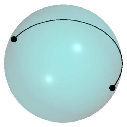
\includegraphics{3dfigures/pdf/1cycle.pdf}
\end{center}
It's not very easy to show, but every such $1$-cycle is homologous to each other,
and double of that cycle is homologous to $0$.

As such, $H^1(\RP^2; \Zc2) \cong \Hom(H_1(\RP^2), \Zc2)$, its only nontrivial element $\alpha$
maps each such $1$-cycle to $1$.

\begin{center}
\begin{asy}
	size(3cm);
	fill(scale(2)*unitsquare, orange+opacity(0.2));
	draw((0, 0)--(0, 2), blue, MidArrow);
	draw((2, 2)--(2, 0), blue, MidArrow);
	draw((0, 0)--(2, 0), red, MidArrow);
	draw((2, 2)--(0, 2), red, MidArrow);
	label("$a$", (0, 2), NW);
	label("$b$", (2, 2), NE);
	label("$c$", (0, 0), SW);
	label("$d$", (2, 0), SE);
	draw((0.5, 0)--(0.5, 2), Arrow);
\end{asy}
\end{center}

Consider $\alpha \smile \alpha$. Notice that $\alpha$ acts like both $dx$ and $dy$ at the same time
(both the blue edge and the red edge got assigned the value $1$), so it assigns the value $1$ to the
whole surface of the real projective plane! Thus it's nontrivial.

\begin{exercise}
	Manually compute the cup product $\alpha \smile \alpha$ to verify that.
	(Divide the surface into some triangles. $[a, c, d] + [a, d, b] - [c, c, d] + [c, d, c]$ is a
	working choice. Verify that the boundary is nonzero, but is divisible by $2$.)
\end{exercise}

\section{Relative cohomology pseudo-rings}
For $A \subseteq X$, one can also define a relative cup product
\[ H^k(X,A;R) \times H^\ell(X,A;R) \to H^{k+\ell}(X,A;R). \]
After all, if either cochain vanishes on chains in $A$,
then so does their cup product.
This lets us define \vocab{relative cohomology pseudo-ring}
and \vocab{reduced cohomology pseudo-ring} (by $A = \{\ast\}$), say
\begin{align*}
H^\bullet(X,A;R) &= \bigoplus_{k \ge 0} H^k(X,A; R) \\
\wt H^\bullet(X;R) &= \bigoplus_{k \ge 0} \wt H^k(X;R).
\end{align*}
These are both \textbf{anticommutative pseudo-rings}.
Indeed, often we have $\wt H^0(X;R) = 0$ and thus there is no identity at all.

Once again we have functoriality:
\begin{theorem}
	[Cohomology (pseudo-)rings are functorial]
	Fix a ring $R$ (commutative with $1$).
	Then we have functors
	\begin{align*}
		H^\bullet(-; R) &: \catname{hTop}\op \to \catname{GradedRings} \\
		H^\bullet(-,-; R) &: \catname{hPairTop}\op \to \catname{GradedPseudoRings}.
	\end{align*}
\end{theorem}

Unfortunately, unlike with (co)homology groups,
it is a nontrivial task to determine\footnote{Apart from the method of passing to differential
form and back, that is. You have already computed a wedge product above.} the cup product
for even nice spaces like CW complexes.
So we will not do much in the way of computation.
However, there is a little progress we can make.

\section{Wedge sums}
Our goal is to now compute $\wt H^\bullet(X \vee Y)$.
To do this, we need to define the product of two graded pseudo-rings:
\begin{definition}
	Let $R$ and $S$ be two graded pseudo-rings.
	The \vocab{product pseudo-ring} $R \times S$ is the graded pseudo-ring
	defined by taking the underlying abelian group as
	\[ R \oplus S = \bigoplus_{d \ge 0} (R^d \oplus S^d). \]
	Multiplication comes from $R$ and $S$, followed by
	declaring $r \cdot s = 0$ for $r \in R$, $s \in S$.
\end{definition}
Note that this is just graded version of the product ring
defined in \Cref{ex:product_ring}.
\begin{exercise}
	Show that if $R$ and $S$ are graded rings (meaning they have $1_R$ and $1_S$),
	then so is $R \times S$.
\end{exercise}

Now, the theorem is that:
\begin{theorem}
	[Cohomology pseudo-rings of wedge sums]
	We have
	\[
		\wt H^\bullet(X \vee Y; R)
		\cong \wt H^\bullet(X;R)
		\times \wt H^\bullet(Y;R)
	\]
	as graded pseudo-rings.
\end{theorem}

Knowing just that the rings are isomorphic doesn't help much, it would be much better if you know
what the isomorphism is --- so that in simple cases, you can see for yourself the rings are
isomorphic.

The isomorphism is the most trivial one:
Given $f \in C^\bullet(X \vee Y; R)$ that assigns to each chain $c$ inside $X \vee Y$ a value
$f(c) \in R$, we can interpret it as an element of $C^\bullet(X)$, because each chain inside $X$ is
trivially a chain inside $X \vee Y$ that can be fed into $f$ ---
formally, the embedding $X \injto X \vee Y$ induces
$C_\bullet(X) \injto C_\bullet(X \vee Y)$. The map induces a $\wt H^\bullet(X \vee Y; R)
\to \wt H^\bullet(X; R) \times \wt H^\bullet(Y; R)$, and it respects the ring multiplication i.e.
the cup product.

\begin{example}
	Let $X$ and $Y$ be depicted as in the following figure.
	\begin{center}
	\begin{asy}
		draw(scale(0.5)*shift(1, 1)*unitcircle);
		draw(shift(-1, 0)*unitsquare);
		label("$=$", (1.25, 0.5));
		draw(shift(1.5, 0)*unitsquare);
		label("$\vee$", (2.75, 0.5));
		draw(shift(3, 0)*scale(0.5)*shift(1, 1)*unitcircle);
	\end{asy}
	\end{center}
	Let $f \in \wt H^1(X; \ZZ)$ assigns $f(X) = 2$ to the whole square, and
	$g \in \wt H^1(Y; \ZZ)$ assigns $g(Y) = 3$ to the whole circle.
	Then, of course the element corresponds to $(f, g)$ inside $\wt H^1(X \vee Y)$ would assigns
	$2 + 3 = 5$ to the cocycle corresponding to the whole space $X \vee Y$.
\end{example}

This allows us to resolve the first question posed at the beginning.
Let $X = \CP^2$ and $Y = S^2 \vee S^4$.
We have that
\[ H^\bullet(\CP^2; \ZZ) \cong \ZZ[\alpha] / (\alpha^3). \]
Hence this is a graded ring generated by there elements:
\begin{itemize}
	\ii $1$, in dimension $0$.
	\ii $\alpha$, in dimension $2$.
	\ii $\alpha^2$, in dimension $4$.
\end{itemize}
Next, consider the reduced cohomology pseudo-ring
\[ \wt H^\bullet(S^2 \vee S^4; \ZZ) \cong
	\wt H^\bullet(S^2; \ZZ)
	\oplus \wt H^\bullet(S^4 ; \ZZ).
\]
Thus the absolute cohomology ring $H^\bullet(S^2 \vee S^4 ; \ZZ)$
is a graded ring also generated by three elements.
\begin{itemize}
	\ii $1$, in dimension $0$ (once we add back in the $0$th dimension).
	\ii $a_2$, in dimension $2$ (from $H^\bullet(S^2 ; \ZZ)$).
	\ii $a_4$, in dimension $4$ (from $H^\bullet(S^4 ; \ZZ)$).
\end{itemize}
Each graded component is isomorphic, like we expected.
However, in the former, the product of two degree $2$ generators is
\[ \alpha \cdot \alpha = \alpha^2. \]
In the latter, the product of two degree $2$ generators is
\[ a_2 \cdot a_2 = a_2^2 = 0 \]
since $a_2 \smile a_2 = 0 \in H^\bullet(S^2; \ZZ)$.

Thus $S^2 \vee S^4$ and $\CP^2$ are not homotopy equivalent.

Intuitively, what the proof above says is:
\begin{moral}
	The nontrivial $4$-cocycle $a_4 \in H^4(S^2 \vee S^4; \ZZ)$
	has nothing to do with the $2$-cocycle $a_2$,
	while the $4$-cocycle $\alpha^2 \in H^4(\CP^2)$ is the cup product $\alpha
	\smile \alpha$ of the $2$-cocycle $\alpha$ with itself.
\end{moral}

The exercise below would be much easier to visualize, apart from the fact that $\RP^2$ is
nonorientable --- in fact, we have already seen
above why $\alpha \smile \alpha \neq 0$ for the nonzero element $\alpha \in H^1(\RP^2)$.

\begin{exercise}
	Similarly, show that $S^1 \vee S^2$ and $\RP^2$ are not homotopy equivalent by showing
	$\wt H^\bullet(S^1 \vee S^2; \Zc 2) \not\cong \wt H^\bullet(\RP^2; \Zc 2)$,
	even though each graded component is isomorphic.
\end{exercise}

\section{Cross product}

In this section, we will define the cross product.

\subsection{Motivation}

Roughly speaking, the motivation is the following:
\begin{moral}
	If $X$ has a $m$-dimensional hole and $Y$ has a $n$-dimensional hole, then $X \times Y$ has a
	$(m + n$)-dimensional hole.
\end{moral}
Which is true in most common cases under suitable interpretation of ``holes''
(either with homology, or with cohomology).

We will formalize and prove the statement above.

\subsection{Cross product on singular homology}

First, we define the \vocab{cross product}, that takes a $m$-simplex $f \colon \Delta^m \to X$ and a
$n$-simplex $g \colon \Delta^n \to Y$, and returns a $(m + n)$-chain $f \times g \in C_{m + n}(X
\times Y)$.\footnote{As far as I know, this is just because the symbol $\times$ is a cross, and it
has nothing to do with the cross product of vectors in $\RR^3$.}
This is really the most natural way you might define it: intuitively, the product of a
$m$-dimensional cube in $X$ and a $n$-dimensional cube in $Y$ is a $(m + n)$-dimensional cube in $X
\times Y$.
\begin{center}
\begin{asy}
	draw((0.5, 0)--(2.5, 0), L=Label("$X$", EndPoint, align=NE));
	draw((0, 0.5)--(0, 2.5), L=Label("$Y$", EndPoint, align=NE));
	draw((1, 0)--(2, 0), blue+1, L=Label("$U$", EndPoint, align=NE));
	dot((1, 0), blue);
	dot((2, 0), blue);
	draw((0, 1)--(0, 2), blue+1, L=Label("$V$", EndPoint, align=NE));
	dot((0, 1), blue);
	dot((0, 2), blue);
	filldraw(shift(1, 1)*unitsquare, blue+opacity(0.1), blue);
	label("$U \times V$", (2, 2), blue, align=N);
	draw(shift(0.5, 0.5)*scale(2)*unitsquare);
	label("$X \times Y$", (2.5, 2.5), align=N);
\end{asy}
\end{center}

In the case of a simplex, we need to subdivide $\Delta^m \times \Delta^n$ into finitely many copies
of $\Delta^{m + n}$.

If $n = 1$, we have already seen a subdivision when we worked with the prism operator. For the
general case, refer to \cite[page 277]{ref:hatcher} --- the number blows up quickly, for example,
you need $\binom{30}{15}=155117520$ simplices to cover $\Delta^{15} \times \Delta^{15}$!

Formally, we can define the cross product of chains: that is, a function
\[ C_m(X) \times C_n(Y) \taking\times C_{m \times n}(X \times Y). \]
We can prove that this induces a map on homology groups:
\[ H_m(X) \times H_n(Y) \taking\times H_{m \times n}(X \times Y). \]

\begin{exercise}
	Let $X = Y = S^1$, so that $X \times Y$ is a torus.
	Let $\alpha$ be a generator of $H_1(X)$, and $\beta$ be a generator of $H_1(Y)$.
	Show that $\alpha \times \beta$ is the generator of $H_2(X \times Y)$.
\end{exercise}

Actually, we have the following:
\begin{theorem}
	\label{thm:topological_kunneth_1}
	% theorem 3B.6 in Hatcher, specialized
If $X$ and $Y$ are CW complexes and $R$ is a PID, then the cross product of two nonzero elements in
$H_m(X)$ and $H_n(Y)$ is nonzero.
\end{theorem}

Thus formalize our intuition earlier --- at least, if we use homology as a measure of ``holes''.

\subsection{Cross product is not a $\ZZ$-module homomorphism}

For this section, if $a$ and $b$ are elements of the $\ZZ$-module $C_m(X)$ and $C_n(Y)$ respectively,
we write $\times(a, b)$ to mean $a \times b \in C_{m + n}(X \times Y)$, and $(a, b)$
to be the element that corresponds in the product $C_m(X) \times C_n(Y)$.

There is a little technical detail that we need to sort out --- above, we writes
\[ \times \colon C_m(X) \times C_n(Y) \to C_{m + n}(X \times Y). \]
But written this way, $\times$ is not a $\ZZ$-module homomorphism!

\begin{example}
	Let $a$ and $b$ be any nonzero elements in $C_m(X)$ and $C_n(Y)$ respectively.

	Then,
	\begin{align*}
		\times(a, b) &= a \times b \\
		2 \cdot (a, b) &= (2a, 2b) \\
		\times(2 \cdot (a, b)) &= 4(a \times b).
	\end{align*}
\end{example}

If we want to talk about isomorphism, or do anything with the $\ZZ$-module structure of $C_{m + n}(X
\times Y)$ or $H_{m + n}(X \times Y)$, we'd better having a $\ZZ$-module homomorphism.

This is easy enough to fix: $\times$ is bilinear, so it's natural to consider the tensor product:
\[ \times \colon C_m(X) \otimes_\ZZ C_n(Y) \to C_{m + n}(X \times Y). \]
With this notation, $\times(a \otimes b) = a \times b$.
(As a side effect, we can also write
$\times(a \otimes b + c \otimes d) = a \times b + c \times d$ now.)

And so, let us restate \Cref{thm:topological_kunneth_1}:
\begin{theorem}
	If $X$ and $Y$ are CW complexes, then
	\[ \times \colon H_m(X) \otimes_\ZZ H_n(Y) \to H_{m + n}(X \times Y) \]
	is an injective $\ZZ$-module homomorphism.
\end{theorem}

\subsection{Cross product on cellular homology}

The definition with singular homology is quite clumsy ---
because we use simplices as the building blocks for the chains,
the product of two simplices in $X$ and $Y$ becomes a huge collection of simplices in $X \times Y$.

We will now redefine the cross product using cellular homology ---
it can be safely skipped, since both definitions of the cross product gives identical result on the
homology groups.

If $X$ and $Y$ are CW complexes, we can do better.
We see that $X \times Y$ has a natural CW complex structure: for each cell $e^m$ of $X$ and cell
$e^n$ of $Y$, their product makes for a cell $e^{m + n}$ of $X \times Y$.

\begin{example}
	If $X$ and $Y$ are both line segments built from
	two $0$-cells and one $1$-cell, then their product $X \times Y$ has a natural CW complex
	structure containing:
	\begin{itemize}
		\ii $4$ $0$-cells,
		\ii $4$ $1$-cells,
		\ii $1$ $2$-cell.
	\end{itemize}
\end{example}

Recall the cellular groups $\Cells_\bullet(X)$ from \Cref{ch:cellular_homology}, each basis element
corresponds to a cell in $X$.
Then, we can define the cross product on the basis elements:
\[ \times \colon \Cells_m(X) \otimes_\ZZ \Cells_n(Y) \to \Cells_{m + n}(X \times Y). \]
To be painfully explicit:
let $e^m \in \Cells_m(X)$, $e^n \in \Cells_m(Y)$, then the cross product is defined by $e^m \times
e^n = e^m \times e^n \in \Cells_{m + n}(X \times Y)$ --- even the notation used is trivial.

Of course, this induces a map on the homology groups:
\[ \times \colon H_m(X) \otimes_\ZZ H_n(Y) \to H_{m + n}(X \times Y). \]
This map is the same as the map we defined earlier.

\subsection{Cross product on cellular cohomology}

We do the same thing as above, but this time with cohomology --- remember that homology and
cohomology are slightly different measures of ``holes'', for $K$ the Klein bottle then $H_2(X) =
0$ but $H^2(X; \ZZ) \neq 0$.

Given two cellular cochains $f \in \Hom(\Cells_m(X); R)$ and
$g \in \Hom(\Cells_n(Y); R)$, we want to obtain a cochain $f
\times g \in \Hom(\Cells_{m + n}(X \times Y); R)$.

Of course, it is defined in the most natural way possible: for a cell $e^m$ of $X$ and a cell $e^n$
of $Y$, we have $(f \times g)(e^m \times e^n) = f(e^m) \cdot g(e^n)$.

Sounds good? Not yet --- since not all $(m + n)$-cells $e^{m + n}$ of $X \times Y$
is formed as a product of a $m$-cell in $X$ and a $n$-cell in $Y$.
For those, we simply declare that $(f \times g)(e^{m + n}) = 0$.

As usual, this map induces a $R$-module homomorphism on the cohomology groups:
\[ \times \colon H^m(X; R) \otimes_R H^n(Y; R) \to H^{m + n}(X \times Y; R). \]

\subsection{Motivation: cross product of differential forms}

The definition of the cross product of two cellular cochains above are clean, but may appear to be
dry and unmotivated.

Turns out you can do the same thing on differential form.
What's more, it gives a clean way of defining the wedge product $\alpha \wedge \beta$!
Let's see it in action.

Instead of the definition, here are a few examples. Motivated readers may try to define the concept
formally.
\begin{example}[Examples of cross product of differential form]
	Here are a few examples.
	\begin{itemize}
		\ii If $X$ and $Y$ are the $x$-axis and the $y$-axis of the plane respectively,
		the cross product $dx \times 2dy$ is equal to $2(dx \wedge dy)$.

		Certainly this is natural --- as $dx$ assigns the value $1$ to the vector $\ee_1$,
		and $2dy$ assigns the value $2$ to the vector $\ee_2$, we get that $dx \times 2dy$ should
		assigns the value $1 \cdot 2 = 2$ to the unit square spanned by $\ee_1$ and $\ee_2$ --- that
		is, $\ee_1 \wedge \ee_2$.
		\ii Let $X$ be the $xy$-plane, and let $Y$ be the $z$-axis.
		Consider the cross product $dx \times dz$. What $2$-form should the result be?

		Certainly, we should have $(dx \times dz)(\ee_1 \wedge \ee_3) = 1$
		and $(dx \times dz)(\ee_2 \wedge \ee_3) = 0$.
		But this isn't enough to uniquely determines $dx \times dz$.

		And so, we declares: $(dx \times dz)(\ee_1 \wedge \ee_2) = 0$.
		With this, we get $dx \times dz = dx \wedge dz$.
	\end{itemize}
\end{example}

More generally, we can define the cross product by picking a basis for $X$ and $Y$, and define the
value of $\alpha \times \beta$ on the basis elements.

As promised --- you can define the wedge product using the cross product.
There's only one thing you can do:
\begin{definition}[Definition of wedge product using the cross product]
	For $X$ a $\RR$-vector space,
	let $\alpha \in (\bigwedge^m(X))^\vee$ and $\beta \in (\bigwedge^n(X))^\vee$,
	then $\alpha \wedge \beta \in (\bigwedge^{m + n}(X)$ is defined by
	\[
		\alpha \wedge \beta = \Delta^*(\alpha \times \beta)
	\]
	where $\Delta \colon X \to X \times X$, $\Delta(x) = (x, x)$ is the diagonal map.
	Recall that $\Delta^*$ denotes the pullback operation.
\end{definition}
In simpler terms:
to evaluate $\alpha \wedge \beta$ on a $(m + n)$-wedge in $X$,
push it to $X \times X$ using the diagonal map, and give it to $\alpha \times \beta$.

\subsection{Piecing the cohomology groups together}

Recall that we have above the $R$-module homomorphism
\[ \times \colon H^m(X; R) \otimes_R H^n(Y; R) \to H^{m + n}(X \times Y; R). \]
We know that it is in fact possible to piece all the $H^\bullet(X; R)$ together to form
an anticommutative graded ring, the cohomology ring. So we wish to extend the map to a
$R$-algebra homomorphism
\[ \times \colon H^\bullet(X; R) \otimes_R H^\bullet(Y; R) \to H^\bullet(X \times Y; R). \]

We haven't defined what the tensor product of two graded rings is yet --- we will formally do that
in the next section, but intuitively, it consists of all the $H^m(X; R) \otimes_R H^n(Y; R)$
pieced together.

\section{K\"unneth formula}
We now wish to tell apart the spaces $S^2 \times S^4$ and $\CP^3$.
In order to do this, we will need a formula
for $H^n(X \times Y; R)$ in terms of $H^n(X;R)$ and $H^n(Y;R)$.
These formulas are called \vocab{K\"unneth formulas}.
In this section we will only use a very special case,
which involves the tensor product of two graded rings.

\begin{definition}
	Let $A$ and $B$ be two graded rings which are also $R$-modules
	(where $R$ is a commutative ring with $1$).
	We define the \vocab{tensor product} $A \otimes_R B$ as follows.
	As an abelian group, it is
	\[ A \otimes_R B = \bigoplus_{d \ge 0}
		\left( \bigoplus_{k=0}^{d} A^k \otimes_R B^{d-k}  \right). \]
	The multiplication is given on basis elements by
	\[ \left( a_1 \otimes b_1 \right)\left( a_2 \otimes b_2 \right)
		= (a_1a_2) \otimes (b_1b_2).
	\]
	Of course the multiplicative identity is $1_A \otimes 1_B$.
\end{definition}

Now let $X$ and $Y$ be topological spaces, and take the product:
we have a diagram
\begin{center}
\begin{tikzcd}
	& X \times Y \ar[ld, "\pi_X"'] \ar[rd, "\pi_Y"] \\
	X && Y
\end{tikzcd}
\end{center}
where $\pi_X$ and $\pi_Y$ are projections.
As $H^k(-; R)$ is functorial, this gives induced maps
\begin{align*}
	\pi_X^\ast &: H^k(X \times Y; R) \to H^k(X; R) \\
	\pi_Y^\ast &: H^k(X \times Y; R) \to H^k(Y; R)
\end{align*}
for every $k$.

By using this, we can define a so-called cross product.
\begin{definition}
	Let $R$ be a ring, and $X$ and $Y$ spaces.
	Let $\pi_X$ and $\pi_Y$ be the projections of $X \times Y$
	onto $X$ and $Y$.
	Then the \vocab{cross product} is the map
	\[
		H^\bullet(X; R) \otimes_R H^\bullet(Y;R)
		\taking{\times} H^\bullet(X \times Y; R)
	\]
	acting on cocycles as follows:
	$\phi \times \psi = \pi_X^\ast(\phi) \smile \pi_Y^\ast(\psi)$.
\end{definition}

This is just the most natural way to take a $k$-cocycle
on $X$ and an $\ell$-cocycle on $Y$, and create a $(k+\ell)$-cocycle
on the product space $X \times Y$.

\begin{remark}
	Of course, this definition coincides with the definition above using cellular cohomology, but
	the proof is omitted.
\end{remark}

\begin{theorem}
	[K\"unneth formula]
	% theorem 3.15 in Hatcher
	Let $X$ and $Y$ be CW complexes such that $H^k(Y;R)$
	is a finitely generated free $R$-module for every $k$.
	Then the cross product is an isomorphism of anticommutative rings
	\[
		H^\bullet(X;R) \otimes_R H^\bullet(Y;R)
		\to H^\bullet(X \times Y; R).
	\]
\end{theorem}

That is:
\begin{moral}
	There is a one-to-one correspondence between pair of holes in $X$ and $Y$
	and holes of $X \times Y$.
	Furthermore, the correspondence respects the cup product.
\end{moral}
Where ``holes'' is to be understood as ``generators of cohomology groups'' in this case.

In any case, this finally lets us resolve the question
set out at the beginning.
We saw that $H_n(\CP^3) \cong H_n(S^2 \times S^4)$ for every $n$,
and thus it follows that $H^n(\CP^3; \ZZ) \cong H^n(S^2 \times S^4; \ZZ)$ too.

But now let us look at the cohomology rings. First, we have
\[ H^\bullet(\CP^3; \ZZ) \cong \ZZ[\alpha] / (\alpha^4)
	\cong \ZZ \oplus \alpha\ZZ \oplus \alpha^2\ZZ \oplus \alpha^3\ZZ
\]
where $|\alpha| = 2$; hence this is a graded ring generated by
\begin{itemize}
	\ii $1$, in degree $0$.
	\ii $\alpha$, in degree $2$.
	\ii $\alpha^2$, in degree $4$.
	\ii $\alpha^3$, in degree $6$.
\end{itemize}

Now let's analyze
\[ H^\bullet(S^2 \times S^4; \ZZ) \cong
	\ZZ[\beta] / (\beta^2)
	\otimes
	\ZZ[\gamma] / (\gamma^2).
\]
It is thus generated thus by the following elements:
\begin{itemize}
	\ii $1 \otimes 1$, in degree $0$.
	\ii $\beta \otimes 1$, in degree $2$.
	\ii $1 \otimes \gamma$, in degree $4$.
	\ii $\beta \otimes \gamma$, in degree $6$.
\end{itemize}
Again in each dimension we have the same abelian group.
But notice that if we square $\beta \otimes 1$ we get
\[ (\beta \otimes 1)(\beta \otimes 1) = \beta^2 \otimes 1 = 0. \]
Yet the degree $2$ generator of $H^\bullet(\CP^3; \ZZ)$
does not have this property.
Hence these two graded rings are not isomorphic.

\begin{moral}
	The nontrivial $4$-cocycle $1 \otimes \gamma$ of $S^2 \times S^4$ is orthogonal to the
	$2$-cocycle $\beta \otimes 1$, while the $4$-cocycle $\alpha^2$ of $\CP^3$ is the cup product
	$\alpha \smile \alpha$ of the $2$-cocycle $\alpha$ with itself.
\end{moral}

So it follows that $\CP^3$ and $S^2 \times S^4$ are not homotopy equivalent.

\begin{exercise}
	Do the same procedure with $H^\bullet(\RP^3; \Zc 2)$ and $H^\bullet(S^1 \times S^2; \Zc 2)$.
	(Visualize $S^1 \times S^2$ as a thickened sphere with the outer and inner face fused together,
	and $RP^3$ as a closed $3$-ball with opposing points on the boundary surface fused together.
	Try to stretch your mind and guess what the homology and cohomology groups are before formally
	compute it.)
\end{exercise}

% Borsuk Ulam

\section\problemhead

\begin{dproblem}
	[Symmetry of Betti numbers by Poincar\'e duality]
	\label{prob:betti}
	Let $M$ be a smooth oriented compact $n$-manifold,
	and let $b_k$ denote its Betti number.
	Prove that $b_k = b_{n-k}$.
	\begin{hint}
		Write $H^k(M; \ZZ)$ in terms of $H_k(M)$
		using the UCT, and analyze the ranks.
	\end{hint}
\end{dproblem}

\begin{problem}
	Show that $\RP^n$ is not orientable for even $n$.
	\begin{hint}
		Use the previous result on Betti numbers.
	\end{hint}
\end{problem}

\begin{problem}
	Show that $\RP^3$ is not homotopy equivalent to $\RP^2 \vee S^3$.
	\begin{hint}
		Use the $\Zc2$ cohomologies, and find the cup product.
	\end{hint}
\end{problem}

\begin{problem}
	\onechili
	Show that $S^m \vee S^n$ is not a deformation retract
	of $S^m \times S^n$ for any $m,n \ge 1$.
	\begin{hint}
		Assume that $r \colon S^m \times S^n \to S^m \vee S^n$ is such a map.
		Show that the induced map
		$H^\bullet(S^m \vee S^n; \ZZ) \to H^\bullet(S^m \times S^n; \ZZ)$
		between their cohomology rings is monic
		(since there exists an inverse map $i$).
	\end{hint}
	\begin{sol}
		See \cite[Example 3.3.14, pages 68-69]{ref:maxim752}.
	\end{sol}
\end{problem}


\part{Algebraic Geometry I: Classical Varieties}
\label{part:ag1}
\parttoc
\chapter{Affine varieties}
In this chapter we introduce affine varieties.
We introduce them in the context of coordinates,
but over the course of the other chapters
we'll gradually move away from this perspective to
viewing varieties as ``intrinsic objects'',
rather than embedded in coordinates.

For simplicity, we'll do almost everything over the field of complex numbers,
but the discussion generalizes to any algebraically closed field.

\section{Affine varieties}
\prototype{$\VV(y-x^2)$ is a parabola in $\Aff^2$.}
%An \vocab{affine variety} is just the zero locus of a set of polynomials.
%We think of it as living in the $n$-dimensional space $\Aff^n$.

\begin{definition}
	Given a set of polynomials $S \subseteq \CC[x_1, \dots, x_n]$
	(not necessarily finite or even countable),
	we let $\VV(S)$ denote the set of points vanishing on \emph{all}
	the polynomials in $S$.
	Such a set is called an \vocab{affine variety}.
	It lives in \vocab{$n$-dimensional affine space}, denoted $\Aff^n$
	(to distinguish it from projective space later).
\end{definition}
For example, a parabola is the zero locus of the polynomial $\VV(y-x^2)$. Picture:
\begin{center}
	\begin{asy}
		import graph;
		size(5cm);

		real f(real x) { return x*x; }
		graph.xaxis("$x$");
		graph.yaxis("$y$");
		draw(graph(f,-2,2,operator ..), blue, Arrows);
		label("$\mathcal V(y-x^2)$", (0.8, f(0.8)), dir(-45), blue);
		label("$\mathbb A^2$", (2,3), dir(45));
	\end{asy}
\end{center}

\begin{example}[Examples of affine varieties]
	These examples are in two-dimensional space $\Aff^2$,
	whose points are pairs $(x,y)$.
	\begin{enumerate}[(a)]
	\ii A straight line can be thought of as $\VV(Ax + By + C)$.
	\ii A parabola as above can be pictured as $\VV(y-x^2)$.
	\ii A hyperbola might be the zero locus of the polynomial $\VV(xy-1)$.
	\ii The two axes can be thought of as $\VV(xy)$; this is the set of points
	such that $x=0$ \emph{or} $y=0$.
	\ii A point $(x_0, y_0)$ can be thought of as $\VV(x-x_0, y-y_0)$.
	\ii The entire space $\Aff^2$ can be thought of as $\VV(0)$.
	\ii The empty set is the zero locus of the constant polynomial $1$, that is $\VV(1)$.
	\end{enumerate}
\end{example}

\section{Naming affine varieties via ideals}
\prototype{$\VV(I)$ is a parabola, where $I=(y-x^2)$.}
As you might have already noticed, a variety can be named by $\VV(-)$ in multiple ways.
For example, the set of solutions to
\[ x=3 \text{ and } y=4 \]
is just the point $(3,4)$.
But this is also the set of solutions to
\[ x=3 \text{ and } y=x+1. \]
So, for example
\[ \{(3,4)\}
	= \VV(x-3, y-4)
	= \VV(x-3, y-x-1).
	\]
That's a little annoying, because in an ideal\footnote{Pun not intended
	but left for amusement value.}
world we would have \emph{one} name
for every variety.
Let's see if we can achieve this.

A partial solution is to use \emph{ideals} rather than small sets.
That is, consider the ideal
\[
	I = \left( x-3, y-4 \right)
	= \left\{ p(x,y) \cdot (x-3) + q(x,y) \cdot (y-4)
	\mid p,q \in \CC[x,y] \right\}
\]
and look at $\VV(I)$.
\begin{ques}
	Convince yourself that $\VV(I) = \{(3,4)\}$.
\end{ques}
So rather than writing $\VV(x-3, y-4)$ it makes sense to
think about this as $\VV\left( I \right)$, where $I = (x-3,y-4)$ is the \emph{ideal}
generated by the two polynomials $x-3$ and $y-4$.
This is an improvement because
\begin{ques}
	Check that $(x-3, y-x-1) = (x-3, y-4)$.
\end{ques}

Needless to say, this pattern holds in general.
\begin{ques}
	Let $\{f_i\}$ be a set of polynomials, and consider
	the ideal $I$ generated by these $\{f_i\}$.
	Show that $\VV(\{f_i\}) = \VV(I)$.
\end{ques}

Thus we will only consider $\VV(I)$ when $I$ is an ideal.
Of course, frequently our ideals are generated by one or two polynomials,
which leads to:
\begin{abuse}
	Given a set of polynomials $f_1, \dots, f_m$
	we let $\VV(f_1, \dots, f_m)$ be shorthand for
	$\VV\left( \left( f_1, \dots, f_m \right) \right)$.
	In other words we let $\VV(f_1, \dots, f_m)$
	abbreviate $\VV(I)$, where $I$ is the \emph{ideal} $I=(f_1, \dots, f_m)$.
\end{abuse}

This is where the Noetherian condition really shines:
it guarantees that every ideal $I \subseteq \CC[x_1, \dots, x_n]$
can be written in the form above with \emph{finitely} many polynomials,
because it is \emph{finitely generated}.
(The fact that $\CC[x_1, \dots, x_n]$ is Noetherian follows from the Hilbert basis theorem,
which is \Cref{thm:hilbert_basis}).
This is a relief, because dealing with infinite sets of polynomials is not much fun.

\section{Radical ideals and Hilbert's Nullstellensatz}
\prototype{$\sqrt{(x^2)} = (x)$ in $\CC[x]$, $\sqrt{(12)} = (6)$ in $\ZZ$.}
You might ask whether the name is unique now:
that is, if $\VV(I) = \VV(J)$, does it follow that $I=J$?
The answer is unfortunately no: the counterexample can be found in just $\Aff^1$.
It is
\[ \VV(x) = \VV(x^2). \]
In other words, the set of solutions to $x=0$
is the same as the set of solutions to $x^2=0$.

Well, that's stupid.
We want an operation which takes the ideal $(x^2)$ and makes it into the ideal $(x)$.
The way to do so is using the radical of an ideal.

\begin{definition}
	Let $R$ be a ring.
	The \vocab{radical} of an ideal $I \subseteq R$, denoted $\sqrt I$,
	is defined by
	\[ \sqrt I = \left\{ r \in R
			\mid r^m \in I \text{ for some integer $m \ge 1$} \right\}. \]
	If $I = \sqrt I$, we say the ideal $I$ itself is \vocab{radical}.
\end{definition}
For example, $\sqrt{(x^2)} = (x)$.
You may like to take the time to verify that $\sqrt I$ is actually an ideal.

\begin{remark}
	[Number theoretic motivation]
	This is actually the same as the notion of ``radical'' in number theory.
	In $\ZZ$, the radical of an ideal $(n)$ corresponds to just
	removing all the duplicate prime factors, so for example
	\[ \sqrt{(12)} = (6). \]
	In particular, if you try to take $\sqrt{(6)}$,
	you just get $(6)$ back;
	you don't squeeze out any new prime factors.

	This is actually true more generally,
	and there is a nice corresponding alternate definition:
	for any ideal $I$, we have
	\[ \sqrt I = \bigcap_{I \subseteq \kp \text{ prime}} \kp. \]
	Although we could prove this now,
	it will be proved later in \Cref{thm:radical_intersect_prime},
	when we first need it.
\end{remark}

Here are the immediate properties you should know.
\begin{proposition}
	[Properties of radical]
	\label{prop:radical}
	In any ring:
	\begin{itemize}
		\ii If $I$ is an ideal, then $\sqrt I$ is always a radical ideal.
		\ii Prime ideals are radical.
		\ii For $I \subseteq \CC[x_1, \dots, x_n]$
		we have $\VV(I) = \VV(\sqrt I)$.
	\end{itemize}
\end{proposition}
\begin{proof}
	These are all obvious.
	\begin{itemize}
		\ii If $f^m \in \sqrt I$ then $f^{mn} \in I$, so $f \in \sqrt I$.
		\ii If $f^n \in \kp$ for a prime $\kp$,
		then either $f \in \kp$ or $f^{n-1} \in \kp$,
		and in the latter case we may continue by induction.
		\ii We have $f(x_1, \dots, x_n) = 0$
		if and only if $f(x_1, \dots, x_n)^m = 0$ for some integer $m$.
		\qedhere
	\end{itemize}
\end{proof}

The last bit makes sense: you would never refer to $x=0$ as $x^2=0$,
and hence we would always want to call $\VV(x^2)$ just $\VV(x)$.
With this, we obtain a theorem called Hilbert's Nullstellensatz.
\begin{theorem}[Hilbert's Nullstellensatz]
	\label{thm:hilbert_null}
	Given an affine variety $V = \VV(I)$,
	the set of polynomials which vanish
	on all points of $V$ is precisely $\sqrt I$.
	Thus if $I$ and $J$ are ideals in $\CC[x_1, \dots, x_n]$, then
	\[ \VV(I) = \VV(J) \text{ if and only if $\sqrt I = \sqrt J$}. \]
\end{theorem}
In other words
\begin{moral}
	Radical ideals in $\CC[x_1, \dots, x_n]$ correspond
	exactly to $n$-dimensional affine varieties.
\end{moral}
The proof of Hilbert's Nullstellensatz will be given in
\Cref{prob:hilbert_from_weak}; for now it is worth remarking that
it relies essentially on the fact that $\CC$ is
\emph{algebraically closed}.
For example, it is false in $\RR[x]$,
with $(x^2+1)$ being a maximal ideal with empty vanishing set.

\section{Pictures of varieties in $\Aff^1$}
\prototype{Finite sets of points (in fact these are the only nontrivial examples).}
Let's first draw some pictures.
In what follows I'll draw $\CC$ as a straight line\dots sorry.

First of all, let's look at just the complex line $\Aff^1$.
What are the various varieties on it?
For starters, we have a single point $9 \in \CC$,
generated by $(x-9)$.

\begin{center}
	\begin{asy}
		size(6cm);
		pair A = (-9,0); pair B = (9,0);
		draw(A--B, Arrows);
		label("$\mathcal V(x-9)$", (0,0), 2*dir(-90), blue);
		dot("$9$", (3,0), dir(90), blue);
		label("$\mathbb A^1$", A+(2,0), dir(90));
	\end{asy}
\end{center}

Another example is the point $4$.
And in fact, if we like we can get an ideal consisting of just these two points;
consider $\VV\left( (x-4)(x-9) \right)$.

\begin{center}
	\begin{asy}
		size(6cm);
		pair A = (-9,0); pair B = (9,0);
		draw(A--B, Arrows);
		label("$\mathcal V( (x-4)(x-9) )$", (0,0), 2*dir(-90), blue);
		dot("$4$", (-1,0), dir(90), blue);
		dot("$9$", (3,0), dir(90), blue);
		label("$\mathbb A^1$", A+(2,0), dir(90));
	\end{asy}
\end{center}

In general, in $\Aff^1$ you can get finitely
many points $\left\{ a_1, \dots, a_n \right\}$ by
just taking \[ \VV\left( (x-a_1)(x-a_2)\dots(x-a_n) \right). \]
On the other hand, you can't get the set $\{0,1,2,\dots\}$ as an affine variety;
the only polynomial vanishing
on all those points is the zero polynomial.
In fact, you can convince yourself that these
are the only affine varieties, with two exceptions:
\begin{itemize}
	\ii The entire line $\Aff^1$ is given by $\VV(0)$, and
	\ii The empty set is given by $\VV(1)$.
\end{itemize}
\begin{exercise}
	Show that these are the only varieties of $\Aff^1$.
	(Let $\VV(I)$ be the variety and pick a $0 \neq f \in I$.)
\end{exercise}

As you might correctly guess, we have:
\begin{theorem}[Intersections and unions of varieties]
	\label{thm:many_aff_variety}
	\listhack
	\begin{enumerate}[(a)]
		\ii The intersection of affine varieties
		(even infinitely many) is an affine variety.
		\ii The union of finitely many affine varieties
		is an affine variety.
	\end{enumerate}
	In fact we have
	\[ \bigcap_\alpha \VV(I_\alpha)
		= \VV\left( \sum_\alpha I_\alpha \right)
		\qquad\text{and}\qquad
		\bigcup_{k=1}^n \VV(I_k)
		= \VV\left( \bigcap_{k=1}^n I_k \right). \]
\end{theorem}
You are welcome to prove this easy result yourself.
\begin{remark}
	Part (a) is a little misleading in that the sum $I+J$ need not be radical:
	take for example $I = (y-x^2)$ and $J = (y)$ in $\CC[x,y]$,
	where $x \in \sqrt{I+J}$ and $x \notin I+J$.
	But in part (b) for radical ideals $I$ and $J$,
	the intersection $I \cap J$ is radical.
\end{remark}

\section{Prime ideals correspond to irreducible affine varieties}
\prototype{$(xy)$ corresponds to the union of two lines in $\Aff^2$.}

Note that most of the affine varieties of $\Aff^1$, like $\{4,9\}$,
are just unions of the simplest ``one-point'' ideals.
To ease our classification,
we can restrict our attention to the case of \emph{irreducible} varieties:
\begin{definition}
	A variety $V$ is \vocab{irreducible} if it cannot be written
	as the union of two proper sub-varieties $V = V_1 \cup V_2$.
\end{definition}
\begin{abuse}
	Warning: in other literature,
	irreducible is part of the definition of variety.
\end{abuse}

\begin{example}
	[Irreducible varieties of $\Aff^1$]
	The irreducible varieties of $\Aff^1$ are:
	\begin{itemize}
		\ii the empty set $\VV(1)$,
		\ii a single point $\VV(x-a)$, and
		\ii the entire line $\Aff^1 = \VV(0)$.
	\end{itemize}
\end{example}
\begin{example}
	[The union of two axes]
	Let's take a non-prime ideal in $\CC[x,y]$, such as $I = (xy)$.
	Its vanishing set $\VV(I)$ is the union of two lines $x=0$ and $y=0$.
	So $\VV(I)$ is reducible.
\end{example}

%We have already seen that the radical ideals
%are in one-to-one correspondence with affine varieties.
%In the next sections we answer the two questions:
%\begin{itemize}
%	\ii What property of $\VV(I)$ corresponds to $I$ being prime?
%	\ii What property of $\VV(I)$ corresponds to $I$ being maximal?
%\end{itemize}
%The first question is easier to answer.

In general:
\begin{theorem}[Prime $\iff$ irreducible]
	Let $I$ be a radical ideal, and $V = \VV(I)$ a nonempty variety.
	Then $I$ is prime if and only if $V$ is irreducible.
\end{theorem}
\begin{proof}
	First, assume $V$ is irreducible; we'll show $I$ is prime.
	Let $f,g \in \CC[x_1, \dots, x_n]$ so that $fg \in I$.
	Then $V$ is a subset of the union $\VV(f) \cup \VV(g)$;
	actually, $V = \left( V \cap \VV(f) \right) \cup \left( V \cap \VV(g) \right)$.
	Since $V$ is irreducible, we may assume $V = V \cap \VV(f)$,
	hence $f$ vanishes on all of $V$. So $f \in I$.

	The reverse direction is similar.
\end{proof}

%\begin{remark}
%	The above proof illustrates the following principle:
%	Let $V$ be an irreducible variety.
%	Suppose that $V \subseteq V_1 \cup V_2$;
%	this implies $V = (V_1 \cap V) \cup (V_2 \cap V)$.
%	Recall that the intersection of two varieties is a variety.
%	Thus an irreducible variety can't even be \emph{contained}
%	in a nontrivial union of two varieties.
%\end{remark}

\section{Pictures in $\Aff^2$ and $\Aff^3$}
\prototype{Various curves and hypersurfaces.}

With this notion, we can now draw pictures in
``complex affine plane'', $\Aff^2$.
What are the irreducible affine varieties in it?

As we saw in the previous discussion,
naming irreducible affine varieties in $\Aff^2$
amounts to naming the prime ideals of $\CC[x,y]$.
Here are a few.
\begin{itemize}
	\ii The ideal $(0)$ is prime. $\VV(0)$ as usual corresponds to the entire plane.
	\ii The ideal $(x-a, y-b)$ is prime,
	since $\CC[x,y] / (x-a, y-b) \cong \CC$ is an integral domain.
	(In fact, since $\CC$ is a field, the ideal $(x-a,y-b)$ is \emph{maximal}).
	The vanishing set of this is $\VV(x-a, y-b) = \{ (a,b) \} \in \CC^2$,
	so these ideals correspond to a single point.
	\ii Let $f(x,y)$ be an irreducible polynomial, like $y-x^2$.
	Then $(f)$ is a prime ideal! Here $\VV(I)$ is a ``degree one curve''.
\end{itemize}

By using some polynomial algebra
(again you're welcome to check this; Euclidean algorithm),
these are in fact the only prime ideals of $\CC[x,y]$.
Here's a picture.

\begin{center}
	\begin{asy}
		import graph;
		graph.xaxis("$x$", -4, 4);
		graph.yaxis("$y$", -4, 4);

		real f (real x) { return x*x; }
		draw(graph(f,-2,2,operator ..), blue);
		label("$\mathcal V(y-x^2)$", (1,1), dir(-45), blue);
		dot("$\mathcal V(x-1,y+2)$", (1,-2), dir(-45), red);
	\end{asy}
\end{center}


As usual, you can make varieties which are just unions of these irreducible ones.
For example, if you wanted the variety consisting of a parabola $y=x^2$
plus the point $(20,15)$ you would write
\[ \VV \left( (y-x^2)(x-20), (y-x^2)(y-15) \right). \]

The picture in $\Aff^3$ is harder to describe.
Again, you have points $\VV(x-a, y-b, z-c)$ corresponding to
be zero-dimensional points $(a,b,c)$, and two-dimensional surfaces
$\VV(f)$ for each irreducible polynomial $f$ (for example, $x+y+z=0$ is a plane).
But there are more prime ideals, like $\VV(x,y)$, which corresponds to the
intersection of the planes $x=0$ and $y=0$: this is the one-dimensional $z$-axis.
It turns out there is no reasonable way to classify the ``one-dimensional'' varieties;
they correspond to ``irreducible curves''.

Thus, as Ravi Vakil \cite{ref:vakil} says:
the purely algebraic question
of determining the prime ideals of $\CC[x,y,z]$
has a fundamentally geometric answer.

\section{Maximal ideals}
\prototype{All maximal ideals are $(x_1-a_1, \dots, x_n-a_n)$.}
We begin by noting:
\begin{proposition}
	[$\VV(-)$ is inclusion reversing]
	If $I \subseteq J$ then $\VV(I) \supseteq \VV(J)$.
	Thus $\VV(-)$ is \emph{inclusion-reversing}.
\end{proposition}
\begin{ques}
	Verify this.
\end{ques}
Thus, bigger ideals correspond to smaller varieties.
As the above pictures might have indicated,
the smallest varieties are \emph{single points}.
Moreover, as you might guess from the name,
the biggest ideals are the \emph{maximal ideals}.
As an example, all ideals of the form
\[ \left( x_1-a_1, \dots, x_n-a_n \right) \]
are maximal, since the quotient
\[ \CC[x_1, \dots, x_n] / \left( x_1-a_1, \dots, x_n-a_n \right) \cong \CC \]
is a field.
The question is: are all maximal ideals of this form?

The answer is in the affirmative.
%It's equivalent to:
%\begin{theorem}
%	[Weak Nullstellensatz, phrased as nonempty varieties]
%	Let $I \subsetneq \CC[x_1, \dots, x_n]$ be a proper ideal.
%	Then the variety $\VV(I) \neq \varnothing$.
%\end{theorem}
% From this we can deduce that all maximal ideals are of the above form.
\begin{theorem}
	[Weak Nullstellensatz, phrased with maximal ideals]
	Every maximal ideal of $\CC[x_1, \dots, x_n]$
	is of the form $(x_1-a_1, \dots, x_n-a_n)$.
\end{theorem}
The proof of this is surprisingly nontrivial,
so we won't include it here yet; see \cite[\S7.4.3]{ref:vakil}.
%% TODO we might include this eventually
%\begin{proof}
%	[WN implies MI]
%	Let $J$ be a maximal ideal, and consider the corresponding variety $V = \VV(J)$.
%	By WN, it contains some point $p=(a_1, \dots, a_n)$.
%	Now, define $I = (x_1-a_1, \dots, x_n-a_n)$; this ideal contains all polynomials
%	vanishing at $p$, so necessarily $J \subseteq I \subsetneq \CC[x_1, \dots, x_n]$.
%	Then by maximality of $J$ we have $J=I$.
%\end{proof}
Again this uses the fact that $\CC$ is algebraically closed.
(For example $(x^2+1)$ is a maximal ideal of $\RR[x]$.)
Thus:
\begin{moral}
	Over $\CC$, maximal ideals correspond to single points.
\end{moral}

Consequently, our various ideals over $\CC$ correspond to various flavors
of affine varieties:
\begin{center}
	\begin{tabular}[h]{|cc|}
		\hline
		Algebraic flavor & Geometric flavor \\ \hline
		radical ideal & affine variety \\
		prime ideal & irreducible variety \\
		maximal ideal & single point \\
		any ideal & (scheme?) \\ \hline
	\end{tabular}
\end{center}
There's one thing I haven't talked about: what's the last entry?

\section{Motivating schemes with non-radical ideals}
One of the most elementary motivations for the scheme
is that we would like to use them to count multiplicity.
That is, consider the intersection
\[ \VV(y-x^2) \cap \VV(y) \subseteq \Aff^2 \]
This is the intersection of the parabola with the tangent $x$-axis,
this is the green dot below.

\begin{center}
	\begin{asy}
		import graph;
		size(5cm);

		real f(real x) { return x*x; }
		graph.xaxis("$x$", red);
		graph.yaxis("$y$");
		draw(graph(f,-2,2,operator ..), blue, Arrows);
		label("$\mathcal V(y-x^2)$", (0.8, f(0.8)), dir(-45), blue);
		label("$\mathbb A^2$", (2,3), dir(45));
		dotfactor *= 1.5;
		dot(origin, heavygreen);
	\end{asy}
\end{center}

Unfortunately, as a variety, it is just a single point!
However, we want to think of this as a ``double point'':
after all, in some sense it has multiplicity $2$.
You can detect this when you look at the ideals:
\[ (y-x^2) + (y) = (x^2,y) \]
and thus, if we blithely ignore taking the radical, we get
\[ \CC[x,y] / (x^2,y) \cong \CC[\eps] / (\eps^2). \]
So the ideals in question are noticing the presence of a double point.

In order to encapsulate this, we need a more refined object than
a variety, which (at the end of the day) is just a set of points;
it's not possible using topology along to encode more information
(there is only one topology on a single point!).
This refined object is the \emph{scheme}.

\section\problemhead
\todo{some actual computation here would be good}

\begin{problem}
	Show that a \emph{real} affine variety $V \subseteq \Aff_\RR^n$
	can always be written in the form $\VV(f)$.
	\begin{hint}
		Squares are nonnegative.
	\end{hint}
	\begin{sol}
		If $V = \VV(I)$ with $I = (f_1, \dots, f_m)$
		(as usual there are finitely many polynomials since $\RR[x_1, \dots, x_n]$ is Noetherian)
		then we can take $f = f_1^2 + \dots + f_m^2$.
	\end{sol}
\end{problem}

\begin{problem}
	[Complex varieties can't be empty]
	\label{prob:complex_variety_nonempty}
	Prove that if $I$ is a proper ideal in $\CC[x_1, \dots, x_n]$
	then $\VV(I) \ne \varnothing$.
	\begin{hint}
		This is actually an equivalent formulation
		of the Weak Nullstellensatz.
	\end{hint}
	\begin{sol}
		Let $I$ be an ideal, and let $\km$ be a maximal ideal contained in it.
		(If you are worried about the existence of $\km$,
		it follows from Krull's Theorem, \Cref{prob:krull_max_ideal}).
		Then $\km = (x_1 - a_1, \dots, x_n - a_n)$ by Weak Nullstellensatz.
		Consequently, $(a_1, \dots, a_n)$ is the unique point of $\VV(\km)$,
		and hence this point is also in $\VV(I)$.
	\end{sol}
\end{problem}

\begin{problem}
	\yod
	\label{prob:hilbert_from_weak}
	Show that Hilbert's Nullstellensatz in $n$ dimensions
	follows from the Weak Nullstellensatz.
	(This solution is called the \vocab{Rabinowitsch Trick}.)
	\begin{hint}
		Use the weak Nullstellensatz on $n+1$ dimensions.
		Given $f$ vanishing on everything,
		consider $x_{n+1}f-1$.
	\end{hint}
	\begin{sol}
		The point is is to check that if $f$ vanishes on all of $\VV(I)$,
		then $f \in \sqrt I$.

		Take a set of generators $f_1, \dots, f_m$,
		in the original ring $\CC[x_1, \dots, x_n]$;
		we may assume it's finite by the Hilbert basis theorem.

		We're going to do a trick now:
		consider $S = \CC[x_1, \dots, x_n, x_{n+1}]$ instead.
		Consider the ideal $I' \subseteq S$ in the bigger ring
		generated by $\{f_1, \dots, f_m\}$ and the polynomial $x_{n+1} f - 1$.
		The point of the last guy is that its zero locus
		does not touch our copy $x_{n+1}=0$ of $\Aff^n$
		nor any point in the ``projection'' of $f$ through $\Aff^{n+1}$
		(one can think of this as $\VV(I)$ in the smaller ring
		direct multiplied with $\CC$).
		Thus $\VV(I') = \varnothing$, and by the weak Nullstellensatz
		we in fact have $I' = \CC[x_1, \dots, x_{n+1}]$.
		So
		\[ 1 = g_1f_1 + \dots + g_mf_m + g_{m+1} \left( x_{n+1}f-1 \right). \]
		Now the hack: \textbf{replace every instance of $x_{n+1}$ by $\frac 1f$},
		and then clear all denominators.
		Thus for some large enough integer $N$ we can get
		\[ f^N = f^N(g_1f_1 + \dots + g_mf_m) \]
		which eliminates any fractional powers of $f$ in the right-hand side.
		It follows that $f^N \in I$.
	\end{sol}
\end{problem}

\chapter{Affine varieties as ringed spaces}
As in the previous chapter, we are working only over affine varieties in $\CC$ for simplicity.

\section{Synopsis}
Group theory was a strange creature in the early 19th century.
During the 19th century, a group was literally defined
as a subset of $\GL(n)$ or of $S_n$.
Indeed, the word ``group'' hadn't been invented yet.
This may sound ludicrous, but it was true -- Sylow developed his theorems without this notion.
Only much later was the abstract definition of a group given,
an abstract set $G$ which was \emph{independent} of any embedding into $S_n$,
and an object in its own right.

We are about to make the same type of change for our affine varieties.
Rather than thinking of them as an object locked into an ambient space $\Aff^n$
we are instead going to try to make them into an object in their own right.
Specifically, for us an affine variety will become a \emph{topological space}
equipped with a \emph{ring of functions} for each of its open sets:
this is why we call it a \textbf{ringed space}.

The bit about the topological space is not too drastic.
The key insight is the addition of the ring of functions.
For example, consider the double point from last chapter.

\begin{center}
	\begin{asy}
		import graph;
		size(5cm);

		real f(real x) { return x*x; }
		graph.xaxis("$x$", red);
		graph.yaxis("$y$");
		draw(graph(f,-2,2,operator ..), blue, Arrows);
		label("$\mathcal V(y-x^2)$", (0.8, f(0.8)), dir(-45), blue);
		label("$\mathbb A^2$", (2,3), dir(45));
		dotfactor *= 1.5;
		dot(origin, heavygreen);
	\end{asy}
\end{center}

As a set, it is a single point,
and thus it can have only one possible topology.
But the addition of the function ring will let us tell it apart
from just a single point.

This construction is quite involved, so we'll proceed as follows:
we'll define the structure bit by bit onto our existing affine varieties in $\Aff^n$,
until we have all the data of a ringed space.
In later chapters, these ideas will grow up to
become the core of modern algebraic geometry: the \emph{scheme}.

\section{The Zariski topology on $\Aff^n$}
\prototype{In $\Aff^1$, closed sets are finite collections of points.
In $\Aff^2$, a nonempty open set is the whole space minus some finite collection of curves/points.}

We begin by endowing a topological structure on every variety $V$.
Since our affine varieties (for now) all live in $\Aff^n$, all we have to do
is put a suitable topology on $\Aff^n$, and then just view $V$ as a subspace.

However, rather than putting the standard Euclidean topology on $\Aff^n$,
we put a much more bizarre topology.
\begin{definition}
	In the \vocab{Zariski topology} on $\Aff^n$,
	the \emph{closed sets} are those of the form
	\[ \VV(I) \qquad\text{where}\quad I \subseteq \CC[x_1, \dots, x_n]. \]
	Of course, the open sets are complements of such sets.
\end{definition}

\begin{example}
	[Zariski topology on $\Aff^1$]
	Let us determine the open sets of $\Aff^1$,
	which as usual we picture as a straight line
	(ignoring the fact that $\CC$ is two-dimensional).

	Since $\CC[x]$ is a principal ideal domain, rather than looking at $\VV(I)$
	for every $I \subseteq \CC[x]$, we just have to look at $\VV(f)$ for a single $f$.
	There are a few flavors of polynomials $f$:
	\begin{itemize}
		\ii The zero polynomial $0$ which vanishes everywhere:
		this implies that the entire space $\Aff^1$ is a closed set.
		\ii The constant polynomial $1$ which vanishes nowhere.
		This implies that $\varnothing$ is a closed set.
		\ii A polynomial $c(x-t_1)(x-t_2)\dots(x-t_n)$ of degree $n$.
		It has $n$ roots, and so $\{t_1, \dots, t_n\}$ is a closed set.
	\end{itemize}
	Hence the closed sets of $\Aff^1$ are exactly all of $\Aff^1$
	and finite sets of points (including $\varnothing$).
	Consequently, the \emph{open} sets of $\Aff^1$ are
	\begin{itemize}
		\ii $\varnothing$, and
		\ii $\Aff^1$ minus a finite collection (possibly empty) of points.
	\end{itemize}
\end{example}

Thus, the picture of a ``typical'' open set $\Aff^1$ might be
\begin{center}
	\begin{asy}
		size(6cm);
		pair A = (-9,0); pair B = (9,0);
		pen bloo = blue+1.5;
		draw(A--B, blue, Arrows);
		draw(A--B, bloo);
		// label("$\mathbb V()$", (0,0), 2*dir(-90));
		opendot((-3,0), bloo);
		opendot((-1,0), bloo);
		opendot((4,0), bloo);
		label("$\mathbb A^1$", B-(2,0), dir(90));
	\end{asy}
\end{center}
It's everything except a few marked points!

\begin{example}[Zariski topology on $\Aff^2$]
	Similarly, in $\Aff^2$,
	the interesting closed sets are going to consist
	of finite unions (possibly empty) of
	\begin{itemize}
		\ii Closed curves,
		like $\VV(y-x^2)$ (which is a parabola), and
		\ii Single points, like $\VV(x-3,y-4)$
		(which is the point $(3,4)$).
	\end{itemize}
	Of course, the entire space $\Aff^2 = \VV(0)$ and the empty set $\varnothing = \VV(1)$
	are closed sets.

	Thus the nonempty open sets in $\Aff^2$ consist of the \emph{entire} plane,
	minus a finite collection of points and one-dimensional curves.
\end{example}
\begin{ques}
	Draw a picture (to the best of your artistic ability)
	of a ``typical'' open set in $\Aff^2$.
\end{ques}

All this is to say
\begin{moral}
	The nonempty Zariski open sets are \emph{huge}.
\end{moral}
This is an important difference than what you're used to in topology.
To be very clear:
\begin{itemize}
	\ii In the past, if I said something like
	``has so-and-so property in an open neighborhood of point $p$'',
	one thought of this as saying
	``is true in a small region around $p$''.
	\ii In the Zariski topology,
	``has so-and-so property in an open neighborhood of point $p$''
	should be thought of as saying ``is true for virtually all points,
	other than those on certain curves''.
\end{itemize}
Indeed, ``open neighborhood'' is no longer really a accurate description.
Nonetheless, in many pictures to follow,
it will still be helpful to draw open neighborhoods as circles.

It remains to verify that as I've stated it, the closed sets actually form a topology.
That is, I need to verify briefly that
\begin{itemize}
	\ii $\varnothing$ and $\Aff^n$ are both closed.
	\ii Intersections of closed sets (even infinite) are still closed.
	\ii Finite unions of closed sets are still closed.
\end{itemize}
Well, closed sets are the same as affine varieties,
so we already know this!

\section{The Zariski topology on affine varieties}
\prototype{If $V = \VV(y-x^2)$ is a parabola,
	then $V$ minus $(1,1)$ is open in $V$.
	Also, the plane minus the origin is $D(x) \cup D(y)$.}

As we said before, by considering a variety $V$ as a subspace of $\Aff^n$
it inherits the Zariski topology.
One should think of an open subset of $V$ as
``$V$ minus a few Zariski-closed sets''.
For example:
\begin{example}[Open set of a variety]
	Let $V = \VV(y-x^2) \subseteq \Aff^2$ be a parabola,
	and let $U = V \setminus \{(1,1)\}$. We claim $U$ is open in $V$.
	\begin{center}
		\begin{asy}
		import graph;
		size(5cm);

		real f(real x) { return x*x; }
		graph.xaxis("$x$");
		graph.yaxis("$y$");
		draw(graph(f,-2,2,operator ..), blue, Arrows);
		label("$\mathcal V(y-x^2)$", (0.8, f(0.8)), dir(-45));

		opendot( (1,1), blue+1);
		\end{asy}
	\end{center}
	Indeed, $\tilde U = \Aff^2 \setminus \{(1,1)\}$ is open in $\Aff^2$
	(since it is the complement of the closed set $\VV(x-1,y-1)$),
	so $U = \tilde U \cap V$ is open in $V$.
	Note that on the other hand the set $U$ is \emph{not} open in $\Aff^2$.
\end{example}

We will go ahead and introduce now a definition
that will be very useful later.
\begin{definition}
	Given $V \subseteq \Aff^n$ an affine variety and $f \in \CC[x_1, \dots, x_n]$,
	we define the \vocab{distinguished open set}
	$D(f)$ to be the open set in $V$
	of points not vanishing on $f$:
	\[ D(f) = \left\{ p \in V \mid f(p) \neq 0 \right\} = V \setminus \VV(f). \]
\end{definition}
In \cite{ref:vakil}, Vakil suggests remembering the
notation $D(f)$ as ``doesn't-vanish set''.
\begin{example}
	[Examples of (unions of) distinguished open sets]
	\listhack
	\begin{enumerate}[(a)]
		\ii If $V = \Aff^1$ then $D(x)$ corresponds to a line minus a point.
		\ii If $V = \VV(y-x^2) \subseteq \Aff^2$,
		then $D(x-1)$ corresponds to the parabola minus $(1,1)$.
		\ii If $V = \Aff^2$, then
		$D(x) \cup D(y) = \Aff^2 \setminus \{ (0,0) \}$
		is the punctured plane.
		You can show that this set is \emph{not} distinguished open.
	\end{enumerate}
\end{example}

% There used to be an exercise here about D(f)
% being a distinguished base

%\begin{ques}
%	Give an example of an open set of $\Aff^2$
%	which is not a distinguished open set.
%	(There was one above already.)
%\end{ques}


\section{Coordinate rings}
\prototype{If $V = \VV(y-x^2)$ then $\CC[V] = \CC[x,y]/(y-x^2)$.}

The next thing we do is consider the functions from $V$ to the base field $\CC$.
We restrict our attention to algebraic (polynomial) functions on a variety $V$:
they should take every point $(a_1, \dots, a_n)$ on $V$ to some complex number $P(a_1, \dots, a_n) \in \CC$.
For example, a valid function on a three-dimensional affine variety might be $(a,b,c) \mapsto a$;
we just call this projection ``$x$''.
Similarly we have a canonical projection $y$ and $z$,
and we can create polynomials by combining them,
say $x^2y + 2xyz$.

\begin{definition}
	The \vocab{coordinate ring} $\CC[V]$ of a variety $V$
	is the ring of polynomial functions on $V$.
	(Notation explained next section.)
\end{definition}

At first glance, we might think this is just $\CC[x_1, \dots, x_n]$.
But on closer inspection we realize that \emph{on a given variety},
some of these functions are the same.
For example, consider in $\Aff^2$ the parabola $V = \VV(y-x^2)$.
Then the two functions
\begin{align*}
	V & \to \CC \\
	(x,y) & \mapsto x^2 \\
	(x,y) & \mapsto y
\end{align*}
are actually the same function!
We have to ``mod out'' by the ideal $I$ which generates $V$.
This leads us naturally to:
\begin{theorem}[Coordinate rings correspond to ideal]
	Let $I$ be a radical ideal, and $V = \VV(I) \subseteq \Aff^n$.
	Then \[ \CC[V] \cong \CC[x_1, \dots, x_n] / I.  \]
\end{theorem}
\begin{proof}
	There's a natural surjection as above
	\[ \CC[x_1, \dots, x_n] \surjto \CC[V] \]
	and the kernel is $I$.
\end{proof}
Thus properties of a variety $V$ correspond to properties of the ring $\CC[V]$.

\section{The sheaf of regular functions}
\prototype{Let $V = \Aff^1$, $U = V \setminus \{0\}$. Then $1/x \in \OO_V(U)$ is regular on $U$.}

Let $V$ be an affine variety and let $\CC[V]$ be its coordinate ring.
We want to define a notion of $\OO_V(U)$ for any open set $U$:
the ``nice'' functions on any open subset.
Obviously, any function in $\CC[V]$ will work as a function on $\OO_V(U)$.
However, to capture more of the structure we want to
loosen our definition of ``nice'' function slightly
by allowing \emph{rational} functions.

The chief example is that $1/x$ should be a regular function
on $\Aff^1 \setminus \{0\}$.
The first natural guess is:
\begin{definition}
	Let $U \subseteq V$ be an open set of the variety $V$.
	A \vocab{rational function} on $U$
	is a quotient $f(x) / g(x)$ of two elements $f$ and $g$ in $\CC[V]$,
	where we require that $g(x) \neq 0$ for $x \in U$.
\end{definition}
However, the definition is slightly too restrictive;
we have to allow for multiple representations:
\begin{definition}
	Let $U \subseteq V$ be open.
	We say a function $\phi \colon U \to \CC$ is a \vocab{regular function} if for
	every point $p \in U$, we can find an open set $U_p \subseteq U$ containing $p$
	and a rational function $f_p/g_p$ on $U_p$ such that
	\[ \phi(x) = \frac{f_p(x)}{g_p(x)} \qquad \forall x \in U_p. \]
	In particular, we require $g_p(x) \neq 0$ on the set $U_p$.
	We denote the set of all regular functions on $U$ by $\OO_V(U)$.
\end{definition}

Thus,
\begin{moral}
	$\phi$ is regular on $U$ if it is locally a rational function.
\end{moral}

This definition is misleadingly complicated,
and the examples should illuminate it significantly.
Firstly, in practice, most of the time we will be able to find
a ``global'' representation of a regular function as a quotient,
and we will not need to fuss with the $p$'s.
For example:
\begin{example}
	[Regular functions]
	\listhack
	\begin{enumerate}[(a)]
		\ii Any function in $f \in \CC[V]$ is clearly regular,
		since we can take $g_p = 1$, $f_p = f$ for every $p$.
		So $\CC[V] \subseteq \OO_V(U)$ for any open set $U$.
		\ii Let $V = \Aff^1$, $U_0 = V \setminus \{0\}$.
		Then $1/x \in \OO_V(U_0)$ is regular on $U_0$.
		\ii Let $V = \Aff^1$, $U_{12} = V \setminus \{1,2\}$. Then
		\[ \frac{1}{(x-1)(x-2)} \in \OO_V(U_{12}) \]
		is regular on $U_{12}$.
	\end{enumerate}
\end{example}
The ``local'' clause with $p$'s is still necessary, though.
\begin{example}
	[Requiring local representations]
	\label{ex:local_rep}
	Consider the variety
	\[ V = \VV(ab-cd) \subseteq \Aff^4 \]
	and the open set $U = V \setminus \VV(b,d)$.
	There is a regular function on $U$ given by
	\[
		(a,b,c,d)
		\mapsto
		\begin{cases}
			a/d & d \neq 0 \\
			c/b & b \neq 0.
		\end{cases}
	\]
	Clearly these are the ``same function'' (since $ab=cd$),
	but we cannot write ``$a/d$'' or ``$c/b$''
	to express it because we run into divide-by-zero issues.
	That's why in the definition of a regular function,
	we have to allow multiple representations.
\end{example}

In fact, we will see later on that the definition
of a regular function is a special case of a more
general construction called \emph{sheafification},
in which ``presheaves of functions which are $P$'' are transformed
into ``sheaves of functions which are \emph{locally} $P$''.

\section{Regular functions on distinguished open sets}
\prototype{Regular functions on $\Aff^1 \setminus \{0\}$ are $P(x) / x^n$.}
The division-by-zero, as one would expect,
essentially prohibits regular functions on the entire space $V$;
i.e.\ there are no regular functions in $\OO_V(V)$
that were not already in $\CC[V]$.
Actually, we have a more general result which computes the
regular functions on distinguished open sets:
\begin{theorem}
	[Regular functions on distinguished open sets]
	\label{thm:reg_func_distinguish_open}
	Let $V \subseteq \Aff^n$ be an affine variety
	and $D(g)$ a distinguished open subset of it.
	Then
	\[ \OO_V( D(g) ) = \left\{ \frac{f}{g^k}
		\mid f \in \CC[V] \text{ and } k \in \ZZ \right\}.  \]
	In particular, $\OO_V(V) = \OO_V(D(1)) \cong \CC[V]$.
\end{theorem}
The proof of this theorem requires the Nullstellensatz,
so it relies on $\CC$ being algebraically closed.
In fact, a counter-example is easy to find if we replace $\CC$ by $\RR$:
consider $\frac{1}{x^2+1}$.
\begin{proof}
	Obviously, every function of the form $f/g^n$ works,
	so we want the reverse direction.
	This is long, and perhaps should be omitted on a first reading.

	Here's the situation.
	Let $U = D(g)$.
	We're given a regular function $\phi$, meaning at every point $p \in D(g)$,
	there is an open neighborhood $U_p$ on which $\phi$ can be expressed
	as $f_p / g_p$ (where $f_p, g_p \in \CC[V]$).
	Then, we want to construct an $f \in \CC[V]$ and an integer $n$
	such that $\phi = f/g^n$.

	First, look at a particular $U_p$ and $f_p / g_p$.
	Shrink $U_p$ to a distinguished open set $D(h_p)$.
	Then, let $\wt f_p = f_p h_p$ and $\wt g_p = g_p h_p$.
	Thus we have that
	\[ \frac{\wt f_p}{\wt g_p} \text{ is correct on }
		D(h_p) \subseteq U \subseteq X. \]
	The upshot of using the modified $f_p$ and $g_p$ is that:
	\[ \wt f_p \wt g_q = \wt f_q \wt g_p \qquad \forall p,q \in U. \]
	Indeed, it is correct on $D(h_p) \cap D(h_q)$ by definition,
	and outside this set both the left-hand side and right-hand side are zero.

	Now, we know that $D(g) = \bigcup_{p \in U} D(\wt g_p)$, i.e.\
	\[ \VV(g) = \bigcap_{p \in U} \VV(\wt g_p). \]
	So by the Nullstellensatz we know that
	\[ g \in \sqrt{(\wt g_p : p \in U)}
		\implies \exists n : g^n \in (\wt g_p : p \in U). \]
	In other words, for some $n$ and $k_p \in \CC[V]$ we have
	\[ g^n = \sum_p k_p \wt g_p \]
	where only finitely many $k_p$ are not zero.
	Now, we claim that
	\[ f \defeq \sum_p k_p \wt f_p \]
	works.
	This just observes by noting that for any $q \in U$, we have
	\[
		f \wt g_q - g^n \wt f_q
		= \sum_p k_p(\wt f_p \wt g_q - \wt g_p \wt f_q)
		= 0. \qedhere
	\]
\end{proof}
This means that the \emph{global} regular functions
are just the same as those in the coordinate ring:
you don't gain anything new by allowing it to be locally a quotient.
(The same goes for distinguished open sets.)

\begin{example}[Regular functions on distinguished open sets]
	\listhack
	\begin{enumerate}[(a)]
		\ii As said already,
		taking $g=1$ we recover $\OO_V(V) \cong \CC[V]$
		for any affine variety $V$.
		\ii Let $V = \Aff^1$, $U_0 = V \setminus \{0\}$. Then
		\[ \OO_V(U_0)
			= \left\{ \frac{P(x)}{x^n} \mid P \in \CC[x],
			\quad n \in \ZZ \right\}. \]
		So more examples are $1/x$ and $(x+1)/x^3$.
	\end{enumerate}
\end{example}

\begin{ques}
	Why doesn't our theorem on regular functions apply to \Cref{ex:local_rep}?
\end{ques}

The regular functions will become of crucial importance
once we define a scheme in the next chapter.

\section{Baby ringed spaces}
In summary, given an affine variety $V$ we have:
\begin{itemize}
	\ii A structure of a set of points,
	\ii A structure of a topological space $V$ on these points, and
	\ii For every open set $U \subseteq V$, a ring $\OO_V(U)$.
	Elements of the rings are functions $U \to \CC$.
\end{itemize}
Let us agree that:
\begin{definition}
	A \vocab{baby ringed space} is a topological space $X$
	equipped with a ring $\OO_X(U)$ for every open set $U$.
	It is required that elements of the ring $\OO_X(U)$
	are functions $f \colon U \to \CC$;
	we call these the \emph{regular functions} of $X$ on $U$.
\end{definition}
Therefore, affine varieties are baby ringed spaces.
\begin{remark}
	This is not a standard definition. Hehe.
\end{remark}

The reason this is called a ``baby ringed space''
is that in a \emph{ringed space},
the rings $\OO_V(U)$ can actually be \emph{any rings},
but they have to satisfy a set of fairly technical conditions.
When this happens, it's the $\OO_V$ that does all the work;
we think of $\OO_V$ as a type of functor called a \emph{sheaf}.

Since we are only studying affine/projective/quasi-projective varieties
for the next chapters, we will just refer to these as baby ringed spaces
so that we don't have to deal with the entire definition.
The key concept is that we want to think of these varieties
as \emph{intrinsic objects}, free of any embedding.
A baby ringed space is philosophically the correct thing to do.

Anyways, affine varieties are baby ringed spaces $(V, \OO_V)$.
In the next chapter we'll meet projective and quasi-projective
varieties, which give more such examples of (baby) ringed spaces.
With these examples in mind, we will finally lay down
the complete definition of a ringed space,
and use this to define a scheme.

\section\problemhead

\begin{dproblem}
	Show that for any $n \ge 1$ the Zariski topology of $\Aff^n$
	is \emph{not} Hausdorff.
\end{dproblem}

\begin{dproblem}
	Let $V$ be an affine variety,
	and consider its Zariski topology.
	\begin{enumerate}[(a)]
		\ii Show that the Zariski topology is \vocab{Noetherian},
		meaning there is no infinite descending chain
		$Z_1 \supsetneq Z_2 \supsetneq Z_3 \supsetneq \dots$ of closed subsets.
		\ii Prove that a Noetherian topological space is compact.
		Hence varieties are topologically compact.
	\end{enumerate}
\end{dproblem}

\begin{sproblem}
	[Punctured Plane]
	\label{prob:punctured_plane}
	Let $V = \Aff^2$ and let $X = \Aff^2 \setminus \{(0,0)\}$ be the punctured plane
	(which is an open set of $V$).
	Compute $\OO_V(X)$.
\end{sproblem}

\chapter{Projective varieties}
Having studied affine varieties in $\Aff^n$, we now consider $\CP^n$.
We will also make it into a baby ringed space
in the same way as with $\Aff^n$.

\section{Graded rings}
\prototype{$\CC[x_0, \dots, x_n]$ is a graded ring.}
We first take the time to state what a graded ring is,
just so that we have this language to use (now and later).

This definition is the same as \Cref{def:graded_ring}.

\begin{definition}
	A \vocab{graded ring} $R$ is a ring with the following additional structure:
	as an abelian group, it decomposes as
	\[ R = \bigoplus_{d \ge 0} R^d \]
	where $R^0$, $R^1$, \dots, are abelian groups.
	The ring multiplication has the property that
	if $r \in R^d$ and $s \in R^e$, we have $rs \in R^{d+e}$.
	Elements of an $R^d$ are called \vocab{homogeneous elements};
	we write ``$d = \deg r$'' to mean ``$r \in R^d$''.

	We denote by $R^+$ the ideal $R \setminus R^0$ generated by
	the homogeneous elements of nonzero degree,
	and call it the \vocab{irrelevant ideal}.
\end{definition}
\begin{remark}
	For experts: all our graded rings are commutative with $1$.
\end{remark}
\begin{example}
	[Examples of graded rings]
	\listhack
	\begin{enumerate}[(a)]
		\ii The ring $\CC[x]$ is graded by degree: as abelian groups,
		$\CC[x] \cong \CC \oplus x\CC \oplus x^2\CC \oplus \dots$.
		\ii More generally, the polynomial ring $\CC[x_0, \dots, x_n]$
		is graded by degree.
	\end{enumerate}
\end{example}
\begin{abuse}
	The notation $\deg r$ is abusive in the case $r = 0$;
	note that $0 \in R^d$ for every $d$.
	So it makes sense to talk about ``the'' degree of $r$
	except when $r = 0$.
\end{abuse}

We will frequently refer to homogeneous ideals:
\begin{definition}
	An ideal $I \subseteq \CC[x_0, \dots, x_n]$ is \vocab{homogeneous}
	if it can be written as $I = (f_1, \dots, f_m)$
	where each $f_i$ is a homogeneous polynomial.
\end{definition}
\begin{remark}
	If $I$ and $J$ are homogeneous,
	then so are $I+J$, $IJ$, $I \cap J$, $\sqrt I$.
\end{remark}
\begin{lemma}[Graded quotients are graded too]
	Let $I$ be a homogeneous ideal of a graded ring $R$.
	Then
	\[ R/I = \bigoplus_{d \ge 0} R^d / (R^d \cap I) \]
	realizes $R/I$ as a graded ring.
\end{lemma}
Since these assertions are just algebra,
we omit their proofs here.
\begin{remark}
	In some other books, homogeneous ideal (or \vocab{graded ideal}) are sometimes defines as ideals $I$
	such that $I = \bigoplus_{d \ge 0} (R^d \cap I)$ as abelian group.
	In fact, we can verify that graded ideals are precisely the ones such that the quotient is naturally graded.
\end{remark}
\begin{example}
	[Example of a graded quotient ring]
	Let $R = \CC[x,y]$ and set $I = (x^3, y^2)$.
	Let $S = R/I$. Then
	\begin{align*}
		S^0 &= \CC \\
		S^1 &= \CC x \oplus \CC y \\
		S^2 &= \CC x^2 \oplus \CC xy \\
		S^3 &= \CC x^2y \\
		S^d &= 0 \qquad \forall d \ge 4.
	\end{align*}
	So in fact $S = R/I$ is graded,
	and is a six-dimensional $\CC$-vector space.
\end{example}


\section{The ambient space}
\prototype{Perhaps $\Vp(x^2+y^2-z^2)$.}
The set of points we choose to work with is $\CP^n$ this time,
which for us can be thought of as the set of $n$-tuples
\[ \left( x_0 : x_1 : \dots : x_n \right) \]
not all zero, up to scaling.
Equivalently, it is the set of lines through the origin in $\CC^{n+1}$.
Projective space is defined in full in \Cref{sec:top_spaces},
and you should refer there if you aren't familiar with projective space.

The right way to think about it is ``$\Aff^n$ plus points at infinity'':
\begin{definition}
	We define the set
	\[ U_i = \left\{ (x_0 : \dots : x_n) \mid x_i \neq 0  \right\}
		\subseteq \CP^n. \]
	These are called the \vocab{standard affine charts}.
\end{definition}
The name comes from:
\begin{exercise}
	[Mandatory]
	Give a natural bijection from $U_i$ to $\Aff^n$.
	Thus we can think of $\CP^n$ as the affine set $U_i$
	plus ``points at infinity''.
\end{exercise}
\begin{remark}
	In fact, these charts $U_i$ make $\CP^n$ with its usual topology
	into a complex manifold with holomorphic transition functions.
\end{remark}

\begin{example}
	[Colloquially, $\CP^1 = \Aff^1 \cup \{\infty\}$]
	The space $\CP^1$ consists of pairs $(s:t)$,
	which you can think of as representing the complex number $z/1$.
	In particular $U_1 = \{ (z:1) \}$
	is basically another copy of $\Aff^1$.
	There is only one new point, $(1:0)$.
\end{example}

However, like before we want to impose a Zariski topology on it.
For concreteness, let's consider $\CP^2 = \left\{ (x_0 : x_1 : x_2) \right\}$.
We wish to consider zero loci in $\CP^2$, just like we did in affine space,
and hence obtain a notion of a projective variety.

But this isn't so easy: for example,
the function ``$x_0$'' is not a well-defined function on points in $\CP^2$
because $(x_0 : x_1 : x_2) = (5x_0 : 5x_1 : 5x_2)$!
So we'd love to consider these ``pseudo-functions''
that still have zero loci. These are just the homogeneous polynomials $f$,
because $f$ is homogeneous of degree $d$ if and only if
\[
	f(\lambda x_0, \dots, \lambda x_n)
	= \lambda^d f(x_0, \dots, x_n).
\]
In particular, the relation ``$f(x_0, \dots, x_n) = 0$'' is
well-defined if $F$ is homogeneous. Thus, we can say:
\begin{definition}
	If $f$ is homogeneous, we can then define its \vocab{vanishing locus} as
	\[
		\Vp(f)
		= \left\{ (x_0 : \dots : x_n) \mid f(x_0, \dots, x_n) = 0 \right\}.
	\]
\end{definition}

The homogeneous condition is really necessary.
For example, to require ``$x_0 - 1 = 0$'' makes no sense,
since the points $(1:1:1)$ and $(2015:2015:2015)$ are the same.

It's trivial to verify that homogeneous polynomials do exactly what we want;
hence we can now define:
\begin{definition}
	A \vocab{projective variety} in $\CP^n$
	is the common zero locus of an arbitrary
	collection of homogeneous polynomials in $n+1$ variables.
\end{definition}

\begin{example}[A conic in $\CP^2$, or a cone in $\CC^3$]
	Let's try to picture the variety
	\[ \Vp(x^2+y^2-z^2) \subseteq \CP^2 \]
	which consists of the points $[x:y:z]$ such that $x^2+y^2=z^2$.
	If we view this as subspace of $\CC^3$
	(i.e.\ by thinking of $\CP^2$ as the set of lines through the origin),
	then we get a ``cone'':
	\begin{center}
		\includegraphics{media/cone.pdf}
	\end{center}

	If we take the standard affine charts now, we obtain:
	\begin{itemize}
		\ii At $x=1$, we get a hyperbola $\VV(1+y^2-z^2)$.
		\ii At $y=1$, we get a hyperbola $\VV(1+x^2-z^2)$.
		\ii At $z=1$, we get a circle $\VV(x^2+y^2-1)$.
	\end{itemize}
	That said, over $\CC$ a hyperbola and circle
	are the same thing; I'm cheating a little by drawing $\CC$
	as one-dimensional, just like last chapter.
\end{example}
\begin{ques}
	Draw the intersection of the cone above
	with the $z=1$ plane, and check that you do in fact get a circle.
	(This geometric picture will be crucial later.)
\end{ques}

\section{Homogeneous ideals}
Now, the next thing we want to do is define $\Vp(I)$ for an ideal $I$.
Of course, we again run into an issue with things like $x_0-1$ not
making sense.

The way out of this is to use only \emph{homogeneous} ideals.
\begin{definition}
	If $I$ is a homogeneous ideal, we define
	\[ \Vp(I) = \{ x \mid f(x) = 0 \; \forall f \in I\}. \]
\end{definition}
\begin{exercise}
	Show that the notion ``$f(x) = 0 \; \forall f \in I$''
	is well-defined for a homogeneous ideal $I$.
\end{exercise}
So, we would hope for a Nullstellensatz-like theorem
which bijects the homogeneous radical ideals to projective varieties.
Unfortunately:
\begin{example}
	[Irrelevant ideal]
	To crush some dreams and hopes, consider the ideal
	\[ I = (x_0, x_1, \dots, x_n). \]
	This is called the \vocab{irrelevant ideal};
	it is a homogeneous radical yet $\Vp(I) = \varnothing$.
\end{example}

However, other than the irrelevant ideal:
\begin{theorem}
	[Homogeneous Nullstellensatz]
	Let $I$ and $J$ be homogeneous ideals.
	\begin{enumerate}[(a)]
		\ii If $\Vp(I) = \Vp(J) \neq \varnothing$ then $\sqrt I = \sqrt J$.
		\ii If $\Vp(I) = \varnothing$, then either $I = (1)$
		or $\sqrt I = (x_0, x_1, \dots, x_n)$.
	\end{enumerate}
	Thus there is a natural bijection between:
	\begin{itemize}
		\ii projective varieties in $\CP^n$, and
		\ii homogeneous radical ideals of $\CC[x_0, \dots, x_n]$
		except for the irrelevant ideal.
	\end{itemize}
\end{theorem}
\begin{proof}
	For the first part, let $V = \Vp(I)$ and $W = \Vp(J)$
	be projective varieties in $\CP^n$.
	We can consider them as \emph{affine varieties} in $\Aff^{n+1}$
	by using the interpretation of $\CP^n$
	as lines through the origin in $\CC^n$.

	Algebraically, this is done by taking the homogeneous ideals
	$I, J \subseteq \CC[x_0, \dots, x_n]$
	and using the same ideals to cut out \emph{affine} varieties
	$V_{\text{aff}} = \VV(I)$ and $W_{\text{aff}} = \VV(J)$ in $\Aff^{n+1}$.
	For example, the cone $x^2+y^2-z^2=0$ is a conic (a one-dimensional curve)
	in $\CP^2$, but can also be thought of as a cone
	(which is a two-dimensional surface) in $\Aff^3$.

	Then for (a), we have $V_{\text{aff}} = W_{\text{aff}}$,
	so $\sqrt I = \sqrt J$.

	For (b), either $V_{\text{aff}}$ is empty
	or it is just the origin of $\Aff^{n+1}$,
	so the Nullstellensatz implies either $I = (1)$
	or $\sqrt I = (x_0, \dots, x_n)$ as desired.
\end{proof}
Projective analogues of \Cref{thm:many_aff_variety}
(on intersections and unions of varieties) hold verbatim
for projective varieties as well.


\section{As ringed spaces}
\prototype{The regular functions on $\CP^1$ minus a point
are exactly those of the form $P(s/t)$.}
Now, let us make every projective variety $V$ into a baby ringed space.
We already have the set of points, a subset of $\CP^n$.

The topology is defined as follows.
\begin{definition}
	We endow $\CP^n$ with the \vocab{Zariski topology}
	by declaring the sets of the form $\Vp(I)$,
	where $I$ is a homogeneous ideal, to be the closed sets.

	Every projective variety $V$ then inherits the Zariski
	topology from its parent $\CP^n$.
	The \vocab{distinguished open sets} $D(f)$ are $V \setminus \Vp(f)$.
\end{definition}

Thus every projective variety $V$ is now a topological space.
It remains to endow it with a sheaf of regular functions $\OO_V$.
To do this we have to be a little careful.
In the affine case we had a nice little ring of functions,
the coordinate ring $\CC[x_0,\dots,x_n] / I$,
that we could use to provide the numerator and denominators.
So, it seems natural to then define:
\begin{definition}
	The \vocab{homogeneous coordinate ring} of a projective variety
	$V = \Vp(I) \subseteq \CP^n$, where $I$ is homogeneous radical,
	is defined as the ring
	\[ \CC[V] = \CC[x_0, \dots, x_n] / I. \]
\end{definition}
However, when we define a rational function we must impose
a new requirement that the numerator and denominator are the same degree.
\begin{definition}
	Let $U \subseteq V$ be an open set of a projective variety $V$.
	A \vocab{rational function} $\phi$ on a projective variety $V$
	is a quotient $f/g$, where $f,g \in \CC[V]$,
	and $f$ and $g$ are homogeneous of the same degree,
	and $\Vp(g) \cap U = \varnothing$.
	In this way we obtain a function $\phi \colon U \to \CC$.
\end{definition}
\begin{example}
	[Examples of rational functions]
	Let $V = \CP^1$ have coordinates $(s:t)$.
	\begin{enumerate}[(a)]
		\ii If $U = V$, then constant functions $c/1$
		are the only rational functions on $U$.
		\ii Now let $U_1 = V \setminus \{(1:0)\}$.
		Then, an example of a regular function is
		\[ \frac{s^2+9t^2}{t^2} = \left( \frac st \right)^2 + 9. \]
		If we think of $U_1$ as $\CC$
		(i.e.\ $\CP^1$ minus an infinity point, hence like $\Aff^1$)
		then really this is just the function $x^2+9$.
	\end{enumerate}
\end{example}
Then we can repeat the same definition as before:
\begin{definition}
	Let $U \subseteq V$ be an open set of a projective variety $V$.
	We say a function $\phi \colon U \to \CC$ is a \vocab{regular function} if
	for every point $p$, we can find an open set $U_p$ containing $p$
	and a rational function $f_p/g_p$ on $U_p$ such that
	\[ \phi(x) = \frac{f_p(x)}{g_p(x)} \qquad \forall x \in U_p. \]
	In particular, we require $U_p \cap \Vp(g_p) = \varnothing$.
	We denote the set of all regular functions on $U$ by $\OO_V(U)$.
\end{definition}
Of course, the rational functions from the previous example
are examples of regular functions as well.
This completes the definition of a projective variety $V$
as a baby ringed space.

\section{Examples of regular functions}
Naturally, I ought to tell you what the regular functions
on distinguished open sets are; this is an analog to
\Cref{thm:reg_func_distinguish_open} from last time.
\begin{theorem}
	[Regular functions on distinguished open sets for projective varieties]
	\label{thm:proj_reg_func_dist_open}
	Let $V$ be a projective variety, and let $g \in \CC[V]$ be homogeneous
	of \emph{positive degree} (thus $g$ is nonconstant).
	Then
	\[
		\OO_V(D(g))
		= \left\{ \frac{f}{g^r} \mid
		f \in \CC[V] \text{ homogeneous of degree $r\deg g$}
		\right\}.
	\]
\end{theorem}
What about the case $g = 1$?
A similar result holds, but we need the assumption that $V$ is irreducible.
\begin{definition}
	A projective variety $V$ is irreducible
	if it can't be written as the union of two proper (projective) sub-varieties.
\end{definition}
\begin{theorem}
	[Only constant regular functions on projective space]
	Let $V$ be an \emph{irreducible} projective variety.
	Then the only regular functions on $V$ are constant,
	thus we have \[ \OO_V(V) \cong \CC. \]
	This relies on the fact that $\CC$ is algebraically closed.
\end{theorem}
Proofs of these are omitted for now.
\begin{example}
	[Irreducibility is needed above]
	The reason we need $V$ irreducible is otherwise
	we could, for example, take $V$ to be the union of two points;
	in this case $\OO_V(V) \cong \CC^{\oplus 2}$.
\end{example}

\begin{remark}
	It might seem strange that $\OO_V(D(g))$ behaves so differently
	when $g = 1$. One vague explanation is that in a projective variety,
	a distinguished open $D(g)$ looks much like an affine variety if $\deg g > 0$.
	For example, in $\CP^1$ we have $\CP^1 \setminus \{0\} \cong \Aff^1$
	(where $\cong$ is used in a sense that I haven't made precise).
	Thus the claim becomes related to the corresponding affine result.
	But if $\deg g = 0$ and $g \neq 0$, then $D(g)$ is the entire projective variety,
	which does not look affine, and thus the analogy breaks down.
\end{remark}

\begin{example}[Regular functions on $\CP^1$]
	Let $V = \CP^1$, with coordinates $(s:t)$.
	\begin{enumerate}[(a)]
		\ii By \Cref{thm:proj_reg_func_dist_open},
		if $U_1$ is the standard affine chart
		omitting the point $(1:0)$, we have
		$ \OO_V(U_1) = \left\{ \frac{f}{t^n} \mid \deg f = n \right\} $.
		One can write this as
		\[ \OO_V(U_1) \cong \left\{ P(s/t) \mid P \in \CC[x] \right\}
			\cong \OO_{\Aff^1} (\Aff^1). \]
		This conforms with our knowledge that $U_1$
		``looks very much like $\Aff^1$''.
		\ii As $V$ is irreducible, $\OO_V(V) = \CC$:
		there are no nonconstant functions on $\CP^1$.
	\end{enumerate}
\end{example}

\begin{example}
	[Regular functions on $\CP^2$]
	Let $\CP^2$ have coordinates $(x:y:z)$ and
	let $U_0 = \left\{ (x:y:1) \in \CP^2 \right\}$
	be the distinguished open set $D(z)$.
	Then in the same vein,
	\[
		\OO_{\CP^2}(U_0)
		= \left\{ \frac{P(x,y)}{z^n} \mid \deg P = n \right\}
		\cong \left\{ P(x/z, y/z) \mid P \in \CC[x,y] \right\}.
	\]
\end{example}

\section\problemhead
\todo{Problems:}
% should be easy to come up with some explicit examples to play with
 % missing problems
\chapter{Bonus: B\'ezout's theorem}
In this chapter we discuss B\'ezout's theorem.
It makes precise the idea that two degree $d$ and $e$
curves in $\CP^2$ should intersect at ``exactly'' $de$ points.
(We work in projective space so e.g.\ any two lines intersect.)

\section{Non-radical ideals}
\prototype{Tangent to the parabola.}
We need to account for multiplicities.
So we will whenever possible work with homogeneous ideals $I$,
rather than varieties $V$,
because we want to allow the possibility that $I$ is not radical.
Let's see how we might do so.

For a first example, suppose we intersect $y=x^2$ with the line $y=1$;
or more accurately, in projective coordinates of $\CP^2$,
the parabola $zy=x^2$ and $y=z$.
The intersection of the ideals is
\[ (zy-x^2, y-z) = (x^2-z^2, y-z) \subseteq \CC[x,y,z]. \]
So this corresponds to having two points;
this gives two intersection points: $(1:1:1)$ and $(-1:1:1)$.
Here is a picture of the two varieties in the affine $z=1$ chart:
\begin{center}
	\begin{asy}
		import graph;
		size(4cm);
		real f(real x) { return x*x-1; }
		graph.xaxis("$\mathcal V(y-z)$", red);
		draw(graph(f,-2,2,operator ..), blue, Arrows);
		label("$\mathcal V(zy-x^2)$", (1.4, f(1.4)), dir(15), blue);
		label("$\mathbb{CP}^2$", (2,3), dir(45));
		dotfactor *= 1.5;
		dot(dir(0), heavygreen);
		dot(dir(180), heavygreen);
	\end{asy}
\end{center}
That's fine, but now suppose we intersect $zy=x^2$ with the line $y=0$ instead.
Then we instead get a ``double point'':
\begin{center}
	\begin{asy}
		import graph;
		size(4cm);
		real f(real x) { return x*x; }
		graph.xaxis("$\mathcal V(y)$", red);
		draw(graph(f,-2,2,operator ..), blue, Arrows);
		label("$\mathcal V(zy-x^2)$", (1.4, f(1.4)), dir(15), blue);
		label("$\mathbb{CP}^2$", (2,3), dir(45));
		dotfactor *= 1.5;
		dot(origin, heavygreen);
	\end{asy}
\end{center}
The corresponding ideal is this time
\[ (zy-x^2, y) = (x^2,y) \subseteq \CC[x,y,z]. \]
This ideal is \emph{not} radical,
and when we take $\sqrt{(x^2,y)} = (x,y)$ we get the ideal
which corresponds to a single projective point $(0:0:1)$ of $\CP^2$.
This is why we work with ideals rather than varieties:
we need to tell the difference between $(x^2,y)$ and $(x,y)$.

\section{Hilbert functions of finitely many points}
\prototype{The Hilbert function attached to the double point $(x^2,y)$
	is eventually the constant $2$.}
\begin{definition}
	Given a nonempty projective variety $V$, there is a unique
	radical ideal $I$ such that $V = \Vp(I)$.
	In this chapter we denote it by $\II(V)$.
	For an empty variety we set $\II(\varnothing) = (1)$,
	rather than choosing the irrelevant ideal.
\end{definition}
\begin{definition}
	Let $I \subseteq \CC[x_0, \dots, x_n]$ be homogeneous.
	We define the \vocab{Hilbert function} of $I$,
	denoted $h_I \colon \ZZ_{\ge 0} \to \ZZ_{\ge 0}$ by
	\[ h_I(d) = \dim_{\CC} \left( \CC[x_0, \dots, x_n]/I \right)^d \]
	i.e.\ $h_I(d)$ is the dimension of the $d$th graded part of
	$\CC[x_0, \dots, x_n] / I$.
\end{definition}
\begin{definition}
	If $V$ is a projective variety, we set $h_V = h_{\II(V)}$,
	where $I$ is the \emph{radical} ideal satisfying $V = \Vp(I)$.
	If $V = \varnothing$, we choose $I = (1)$.
\end{definition}
\begin{example}[Examples of Hilbert functions in zero dimensions]
	\label{ex:hilbert_zero}
	For concreteness, let us use $\CP^2$.
	\begin{enumerate}[(a)]
		\ii If $V$ is the single point $(0:0:1)$,
		with ideal $\II(V) = (x,y)$,
		then
		\[ \CC[x,y,z] / (x,y) \cong \CC[z]
		\cong \CC \oplus z\CC \oplus z^2\CC \oplus z^3\CC \dots \]
		which has dimension $1$ in all degrees.
		Consequently, we have \[ h_I(d) \equiv 1. \]
		\ii Now suppose we use the ``double point'' ideal $I = (x^2,y)$.
		This time, we have
		\begin{align*}
			\CC[x,y,z] / (x^2,y)
			&\cong \CC[z] \oplus x\CC[z] \\
			&\cong \CC \oplus (x\CC \oplus z\CC) \oplus (xz\CC \oplus z^2\CC)
			\oplus (xz^2\CC \oplus z^3\CC) \oplus\dots.
		\end{align*}
		From this we deduce that
		\[
			h_I(d) =
			\begin{cases}
				2 & d = 1, 2, 3, \dots \\
				1 & d = 0.
			\end{cases}
		\]
		\ii Let's now take the variety $V = \{(1:1:1), (-1:1:1)\}$
		consisting of two points, with $\II(V) = (x^2-z^2, y-z)$. Then
		\begin{align*}
			\CC[x,y,z] / (x^2-z^2,y-z)
			&\cong \CC[x,z] / (x^2-z^2) \\
			&\cong \CC[z] \oplus x\CC[z].
		\end{align*}
		So this example has the same Hilbert function as the previous one.
	\end{enumerate}
\end{example}
\begin{abuse}
	I'm abusing the isomorphism symbol
	$\CC[z] \cong \CC \oplus z\CC \oplus z^2\CC$ and similarly
	in other examples.
	This is an isomorphism only on the level of $\CC$-vector spaces.
	However, in computing Hilbert functions of other examples
	I will continue using this abuse of notation.
\end{abuse}
\begin{example}
	[Hilbert functions for empty varieties]
	Suppose $I \subsetneq \CC[x_0, \dots, x_n]$
	is an ideal, possibly not radical
	but such that \[ \Vp(I) = \varnothing \]
	hence $\sqrt I = (x_0, \dots, x_n)$ is the irrelevant ideal.
	Thus there are integers $d_i$ for $i=0,\dots,n$ such that
	$x_i^{d_i} \in I$ for every $i$; consequently, $h_I(d) = 0$
	for any $d > d_0 + \dots + d_n$.
	We summarize this by saying that
	\[ h_I(d) = 0 \text{ for all $d \gg 0$}. \]
\end{example}
Here the notation $d\gg 0$ means ``all sufficiently large $d$''.

From these examples we see that if $I$ is an ideal,
then the Hilbert function appears to eventually be constant,
with the desired constant equal to the size of $\Vp(I)$,
``with multiplicity'' in the case that $I$ is not radical.

Let's prove this.
Before proceeding we briefly remind the reader of short exact sequences:
a sequence of maps of $0 \to V \injto W \surjto X \to 0$
is one such that the $\img(V \injto W) = \ker(W \surjto X)$
(and of course the maps $V \injto W$ and $W \surjto X$ are
injective and surjective).
If $V$, $W$, $X$ are finite-dimensional vector spaces over $\CC$
this implies that $\dim W = \dim V + \dim X$.

\begin{proposition}
	[Hilbert functions of $I \cap J$ and $I+J$]
	Let $I$ and $J$ be homogeneous ideals in $\CC[x_0, \dots, x_n]$.
	Then \[ h_{I \cap J} + h_{I+J} = h_I + h_J. \]
\end{proposition}
\begin{proof}
	Consider any $d \ge 0$.
	Let $S = \CC[x_0, \dots, x_n]$ for brevity.
	Then
	\begin{center}
	\begin{tikzcd}
		0 \ar[r]
			& \left[ S / (I \cap J) \right]^d \ar[r, hook]
			& \left[ S / I \right]^d \oplus \left[ S / J \right]^d \ar[r, surjective head]
			& \left[ S / (I+J) \right]^d \ar[r] & 0 \\
		& f \ar[r, mapsto] & (f,f) \\
		&& (f,g) \ar[r, mapsto] & f-g
	\end{tikzcd}
	\end{center}
	is a short exact sequence of vector spaces.
	Therefore, for every $d \ge 0$ we have that
	\[
		\dim \left[ S / I \right]^d \oplus \left[ S / J \right]^d
		= \dim \left[ S / (I \cap J) \right]^d
		+ \dim \left[ S / (I+J) \right]^d
	\]
	which gives the conclusion.
\end{proof}
\begin{example}
	[Hilbert function of two points in $\CP^1$]
	In $\CP^1$ with coordinate ring $\CC[s,t]$,
	consider $I = (s)$ the ideal corresponding to the point $(0:1)$
	and $J = (t)$ the ideal corresponding to the point $(1:0)$.
	Then $I \cap J = (st)$ is the ideal corresponding
	to the disjoint union of these two points,
	while $I+J = (s,t)$ is the irrelevant ideal.
	Consequently $h_{I+J}(d) = 0$ for $d \gg 0$.
	Therefore, we get
	\[ h_{I \cap J}(d) = h_I(d) + h_J(d) \text{ for $d \gg 0$} \]
	so the Hilbert function of a two-point projective variety
	is the constant $2$ for $d \gg 0$.
\end{example}

This example illustrates the content of the main result:
\begin{theorem}
	[Hilbert functions of zero-dimensional varieties]
	Let $V$ be a projective variety consisting of $m$ points
	(where $m \ge 0$ is an integer).
	Then \[ h_V(d) = m \text{ for $d \gg 0$}. \]
\end{theorem}
\begin{proof}
	We already did $m = 0$, so assume $m \ge 1$.
	Let $I = \II(V)$ and for $k=1,\dots,m$
	let $I_k = \II(\text{$k$th point of $V$})$.
	\begin{exercise}
		Show that $h_{I_k} (d) = 1$ for every $d$.
		(Modify \Cref{ex:hilbert_zero}(a).)
		\label{ques:hilbert_always_one}
	\end{exercise}

	Hence we can proceed by induction on $m \ge 2$,
	with the base case $m=1$ already done above.
	For the inductive step,
	we use the projective analogues of \Cref{thm:many_aff_variety}.
	We know that $h_{I_1 \cap \dots \cap I_{m-1}}(d) = m-1$ for $d \gg 0$
	(this is the first $m-1$ points;
	note that $I_1 \cap \dots \cap I_{m-1}$ is radical).
	To add in the $m$th point we note that
	\[
		h_{I_1 \cap \dots \cap I_m}(d)
		= h_{I_1 \cap \dots I_{m-1}}(d) + h_{I_m}(d)
		- h_J(d)
	\]
	where $J = (I_1 \cap \dots \cap I_{m-1}) + I_m$.
	The ideal $J$ may not be radical, but satisfies $\Vp(J) = \varnothing$
	by an earlier example, hence $h_J = 0$ for $d \gg 0$.
	This completes the proof.
\end{proof}
In exactly the same way we can prove that:
\begin{corollary}[$h_I$ eventually constant when $\dim \Vp(I) = 0$]
	Let $I$ be an ideal, not necessarily radical,
	such that $\Vp(I)$ consists of finitely many points.
	Then the Hilbert $h_I$ is eventually constant.
\end{corollary}
\begin{proof}
	Induction on the number of points, $m \ge 1$.
	The base case $m = 1$ was essentially done in \Cref{ex:hilbert_zero}(b)
	and \Cref{ques:hilbert_always_one}.
	The inductive step is literally the same as in the proof above,
	except no fuss about radical ideals.
\end{proof}

\section{Hilbert polynomials}
So far we have only talked about Hilbert functions
of zero-dimensional varieties, and showed that
they are eventually constant.
Let's look at some more examples.
\begin{example}
	[Hilbert function of $\CP^n$]
	The Hilbert function of $\CP^n$ is
	\[ h_{\CP^n}(d) = \binom{d+n}{n}
	= \frac{1}{n!} (d+n)(d+n-1) \dots (d+1) \]
	by a ``balls and urns'' argument.
	This is a polynomial of degree $n$.
\end{example}
\begin{example}
	[Hilbert function of the parabola]
	Consider the parabola $zy-x^2$ in $\CP^2$
	with coordinates $\CC[x,y,z]$.
	Then
	\[ \CC[x,y,z] / (zy-x^2) \cong \CC[y,z] \oplus x\CC[y,z]. \]
	A combinatorial computation gives that
	\begin{align*}
		h_{(zy-x^2)}(0) &= 1 & \text{Basis $1$} \\
		h_{(zy-x^2)}(1) &= 3 & \text{Basis $x,y,z$} \\
		h_{(zy-x^2)}(2) &= 5 & \text{Basis $xy$, $xz$, $y^2$, $yz$, $z^2$}.
	\end{align*}
	We thus in fact see that $h_{(zy-x^2)}(d) = 2d-1$.
\end{example}

In fact, this behavior of ``eventually polynomial'' always works.
\begin{theorem}
	[Hilbert polynomial]
	Let $I \subseteq \CC[x_0, \dots, x_n]$ be a homogeneous ideal,
	not necessarily radical. Then
	\begin{enumerate}[(a)]
		\ii There exists a polynomial $\chi_I$ such that
		$h_I(d) = \chi_I(d)$ for all $d \gg 0$.
		\ii $\deg \chi_I = \dim\Vp(I)$ (if $\Vp(I) = \varnothing$
		then $\chi_I = 0$).
		\ii The polynomial $m! \cdot \chi_I$ has integer coefficients.
	\end{enumerate}
\end{theorem}
\begin{proof}
	The base case was addressed in the previous section.

	For the inductive step, consider $\Vp(I)$ with dimension $m$.
	Consider a hyperplane $H$ such that no irreducible
	component of $\Vp(I)$ is contained inside $H$
	(we quote this fact without proof, as it is geometrically obvious,
	but the last time I tried to write the proof I messed up).
	For simplicity, assume WLOG that $H = \Vp(x_0)$.

	Let $S = \CC[x_0, \dots, x_n]$ again.
	Now, consider the short exact sequence
	\begin{center}
	\begin{tikzcd}
		0 \ar[r]
			& \left[ S/I \right]^{d-1} \ar[r, hook]
			& \left[ S / I \right]^d \ar[r, surjective head]
			& \left[ S / (I+(f)) \right]^d \ar[r] & 0 \\
		& f \ar[r, mapsto] & f \cdot x_0 \\
		&& f \ar[r, mapsto] & f.
	\end{tikzcd}
	\end{center}
	(The injectivity of the first map follows from the assumption
	about irreducible components of $\Vp(I)$.)
	Now exactness implies that
	\[ h_I(d) - h_I(d-1) = h_{I + (x_0)}(d). \]
	The last term geometrically corresponds to $\Vp(I) \cap H$;
	it has dimension $m-1$, so by the inductive hypothesis
	we know that
	\[ h_I(d) - h_I(d-1)
		= \frac{c_0 d^{m-1} + c_1 d^{m-2} + \dots + c_{m-1}}{(m-1)!}
		\qquad d \gg 0 \]
	for some integers $c_0$, \dots, $c_{m-1}$.
	Then we are done by the theory of
	\textbf{finite differences} of polynomials.
\end{proof}

\section{B\'ezout's theorem}

\begin{definition}
	We call $\chi_I$ the \vocab{Hilbert polynomial} of $I$.
	If $\chi_I$ is nonzero, we call the leading coefficient of
	$m! \chi_I$ the \vocab{degree} of $I$, which is an integer,
	denoted $\deg I$.

	Of course for projective varieties $V$ we let $h_V = h_{\II(V)}$.
\end{definition}

\begin{example}[Examples of degrees]
	\listhack
	\begin{enumerate}[(a)]
		\ii If $V$ is a finite set of $n \ge 1$ points, it has degree $n$.
		\ii If $I$ corresponds to a double point, it has degree $2$.
		\ii $\CP^n$ has degree $1$.
		\ii The parabola has degree $2$.
	\end{enumerate}
\end{example}

Now, you might guess that if $f$ is a homogeneous quadratic polynomial
then the degree of the principal ideal $(f)$ is $2$, and so on.
(Thus for example we expect a circle to have degree $2$.)
This is true:

\begin{theorem}
	[B\'ezout's theorem]
	Let $I$ be a homogeneous ideal of $\CC[x_0, \dots, x_n]$,
	such that $\dim \Vp(I) \ge 1$.
	Let $f \in \CC[x_0, \dots, x_n]$ be a homogeneous polynomial of degree $k$
	which does not vanish on any irreducible component of $\Vp(I)$.
	Then
	\[ \deg\left( I + (f) \right) = k \deg I. \]
\end{theorem}
\begin{proof}
	Let $S = \CC[x_0, \dots, x_n]$ again.
	This time the exact sequence is
	\begin{center}
	\begin{tikzcd}
		0 \ar[r]
			& \left[ S/I \right]^{d-k} \ar[r, hook]
			& \left[ S / I \right]^d \ar[r, surjective head]
			& \left[ S / (I+(f)) \right]^d \ar[r] & 0.
	\end{tikzcd}
	\end{center}
	We leave this olympiad-esque exercise as \Cref{prob:bezout}.
\end{proof}

\section{Applications}
First, we show that the notion of degree is what we expect.
\begin{corollary}
	[Hypersurfaces: the degree deserves its name]
	Let $V$ be a hypersurface, i.e. $\II(V) = (f)$
	for $f$ a homogeneous polynomial of degree $k$.
	Then $\deg V = k$.
\end{corollary}
\begin{proof}
	Recall $\deg(0) = \deg \CP^n = 1$.
	Take $I = (0)$ in B\'ezout's theorem.
\end{proof}

The common special case in $\CP^2$ is:
\begin{corollary}[B\'ezout's theorem for curves]
	For any two curves $X$ and $Y$ in $\CP^2$ without
	a common irreducible component,
	\[ \left\lvert X \cap Y \right\rvert
		\le \deg X \cdot \deg Y. \]
\end{corollary}

Now, we use this to prove Pascal's theorem.
\begin{theorem}
	[Pascal's theorem]
	Let $A$, $B$, $C$, $D$, $E$, $F$ be six
	distinct points which lie on a conic $\mathscr C$ in $\CP^2$.
	Then the points $AB \cap DE$, $BC \cap EF$, $CD \cap FA$ are collinear.
\end{theorem}
\begin{proof}
	Let $X$ be the variety equal to the union of the
	three lines $AB$, $CD$, $EF$, hence $X = \Vp(f)$
	for some cubic polynomial $f$ (which is the product of three linear ones).
	Similarly, let $Y = \Vp(g)$ be the variety
	equal to the union of the three lines $BC$, $DE$, $FA$.

	\begin{center}
		\begin{asy}
			filldraw(unitcircle, opacity(0.2)+lightcyan, blue);
			pair A = dir(110);
			pair B = dir(210);
			pair C = dir(40);
			pair D = dir(270);
			pair E = dir(130);
			pair F = dir(-30);

			pair P = extension(A, B, D, E);
			pair X = extension(B, C, E, F);
			pair Q = extension(C, D, F, A);

			draw(A--B--C--D--E--F--cycle);
			draw(P--Q, red+dashed);

			dot("$A$", A, dir(A));
			dot("$B$", B, dir(B));
			dot("$C$", C, dir(C));
			dot("$D$", D, dir(D));
			dot("$E$", E, dir(E));
			dot("$F$", F, dir(F));
			dot(P);
			dot(X);
			dot(Q);

			/* Source generated by TSQ */
		\end{asy}
	\end{center}

	Now let $P$ be an arbitrary point on the conic on $\mathscr C$,
	distinct from the six points $A$, $B$, $C$, $D$, $E$, $F$.
	Consider the projective variety
	\[ V = \Vp(\alpha f + \beta g) \]
	where the constants $\alpha$ and $\beta$ are chosen such that $P \in V$.
	\begin{ques}
		Show that $V$ also contains the six points $A$, $B$, $C$, $D$, $E$, $F$
		as well as the three points $AB \cap DE$, $BC \cap EF$, $CD \cap FA$
		regardless of which $\alpha$ and $\beta$ are chosen.
	\end{ques}

	Now, note that $|V \cap \mathscr C| \ge 7$.
	But $\deg V = 3$ and $\deg \mathscr C = 2$.
	This contradicts B\'ezout's theorem unless $V$ and $\mathscr C$
	share an irreducible component.
	This can only happen if $V$ is the union of a line and conic,
	for degree reasons; i.e.\ we must have that
	\[ V = \mathscr C \cup \text{line}. \]
	Finally note that the three intersection points $AB \cap DE$,
	$BC \cap EF$ and $CD \cap FA$ do not lie on $\mathscr C$,
	so they must lie on this line.
\end{proof}


\section\problemhead
\begin{problem}
	\label{prob:bezout}
	Complete the proof of B\'ezout's theorem from before.
	\begin{sol}
		From the exactness,
		$h_I(d) = h_I(d-k) + h_{I+(f)}(d)$,
		and it follows that
		\[ \chi_{I+(f)}(d) = \chi_I(d) - \chi_I(d-k). \]
		Let $m = \dim \Vp(I) \ge 1$.
		Now $\dim \Vp(I+(f)) = m-1$, so
		and $c_{\text{new}} = \deg I+(f)$ then we have
		\[
			\frac{\deg (I+(f)) d^{m-1} + \dots}{(m-1)!}
			=
			\frac{1}{m!}
			\left( \deg I (d^m - (d-k)^m)
			+ \text{lower order terms} \right)
		\]
		from which we read off
		\[ \deg (I+(f)) = \frac{(m-1)!}{m!} \cdot k \binom m1 \deg I
			= k \deg I \]
		as needed.
	\end{sol}
\end{problem}

\begin{problem}
	[USA TST 2016/6]
	\yod
	Let $ABC$ be an acute scalene triangle
	and let $P$ be a point in its interior.
	Let $A_1$, $B_1$, $C_1$ be projections of $P$ onto
	triangle sides $BC$, $CA$, $AB$, respectively.
	Find the locus of points $P$ such that $AA_1$, $BB_1$, $CC_1$
	are concurrent and $\angle PAB + \angle PBC + \angle PCA = 90^{\circ}$.
	\begin{hint}
		You will need to know about complex numbers
		in Euclidean geometry to solve this problem.
	\end{hint}
	\begin{sol}
	In complex numbers with $ABC$ the unit circle,
	it is equivalent to solving the two cubic equations
	\begin{align*}
		(p-a)(p-b)(p-c) &= (abc)^2 (q -1/a)(q - 1/b)(q - 1/c) \\
		0 &= \prod_{\text{cyc}} (p+c-b-bcq) + \prod_{\text{cyc}} (p+b-c-bcq)
	\end{align*}
	in $p$ and $q = \overline p$.
	Viewing this as two cubic curves in $(p,q) \in \mathbb C^2$,
	by B\'{e}zout's theorem it follows there are at most nine solutions
	(unless both curves are not irreducible,
	but one can check the first one cannot be factored).
	Moreover it is easy to name nine solutions (for $ABC$ scalene):
	the three vertices, the three excenters, and $I$, $O$, $H$.
	Hence the answer is just those three triangle centers $I$, $O$ and $H$.
	\end{sol}
\end{problem}

\chapter{Morphisms of varieties}
In preparation for our work with schemes,
we will finish this part by talking about \emph{morphisms}
between affine and projective varieties,
given that we have taken the time to define them.

Idea: we know both affine and projective varieties are special
cases of baby ringed spaces, so in fact we will just define a morphism
between \emph{any} two baby ringed spaces.

\section{Defining morphisms of baby ringed spaces}
\prototype{See next section.}
Let $(X, \OO_X)$ and $(Y, \OO_Y)$ be baby ringed spaces, and think
about how to define a morphism between them.

The guiding principle in algebra is that we want morphisms
to be functions on underlying structure, but also respect
the enriched additional data on top.
To give some examples from the very beginning of time:
\begin{example}
	[How to define a morphism]
	\listhack
	\begin{itemize}
	\ii Consider groups.
	A group $G$ has an underlying set (of elements),
	which we then enrich with a multiplication operation.
	So a homomorphism is a map of the underlying sets,
	plus it has to respect the group multiplication.
	\ii Consider $R$-modules.
	Each $R$-module has an underlying abelian group,
	which we then enrich with scalar multiplication.
	So we require that a linear map respects the scalar multiplication as well,
	in addition to being a homomorphism of abelian groups.
	\ii Consider topological spaces.
	A space $X$ has an underlying set (of points),
	which we then enrich with a topology of open sets.
	So we consider maps of the set of points
	which respect the topology (pre-images of open sets are open).
	\end{itemize}
\end{example}
This time, the ringed spaces $(X, \OO_X)$ have an underlying
\emph{topological space}, which we have enriched with a structure sheaf.
So, we want a continuous map $f \colon X \to Y$ of these topological spaces,
which we then need to respect the sheaf of regular functions.

How might we do this? Well, if we let $\psi \colon Y \to \CC$
be a regular function, then composition gives a natural way to
write a map $X \to Y \to \CC$.
We then want to require that this is also a regular function.

More generally, we can take any regular function on $Y$
and obtain some function on $X$, which we call a pullback.
We then require that all the pullbacks are regular on $X$.
\begin{definition}
	Let $(X, \OO_X)$ and $(Y, \OO_Y)$ be baby ringed spaces.
	Given a map $f \colon X \to Y$ and a regular function $\phi \in \OO_Y(U)$,
	we define the \vocab{pullback} of $\phi$, denoted $f^\sharp\phi$,
	to be the composed function
	\[ f\pre(U) \taking{f} U \taking{\phi} \CC. \]
\end{definition}
The use of the word ``pullback'' is the same as in our study
of differential forms.

\begin{definition}
	Let $(X, \OO_X)$ and $(Y, \OO_Y)$ be baby ringed spaces.
	A continuous map of topological spaces $f \colon X \to Y$
	is a \vocab{morphism} if every pullback of a regular function on $Y$
	is a regular function on $X$.

	Two baby ringed spaces are \vocab{isomorphic}
	if there are mutually inverse morphisms between them,
	which we then call \vocab{isomorphisms}.
\end{definition}

In particular, the pullback gives us a (reversed) \emph{ring homomorphism}
\[ f^\sharp \colon \OO_Y(U) \to \OO_X(f\pre(U)) \] for \emph{every} $U$;
thus our morphisms package a lot of information.
Here's a picture of a morphism $f$,
and the pullback of $\phi \colon U \to \CC$ (where $U \subseteq Y$).
\begin{center}
	\begin{asy}
		size(13cm);
		bigblob("$X$");
		pair p = (0.5,0);
		filldraw(CR(p, 1), opacity(0.2)+lightgreen, deepgreen+dashed);
		label("$f^{\text{pre}}(U)$", p+dir(135), dir(135), deepgreen);

		transform t = scale(0.8) * shift(14*dir(180));
		add(t * CC());
		p = t*p;

		bigblob("$Y$");
		pair q = (0,0.5);
		filldraw(CR(q, 1.2), opacity(0.2)+lightred, red+dashed);
		label("$U$", q+1.2*dir(45), dir(45), red);

		draw( (-9,0.5)--(-3,0.5), EndArrow);
		label("$f$", (-6,0.5), dir(90));

		draw(q--(0,-8), red, EndArrow);
		label("$\phi \in \mathcal O_Y(U)$", (0,-6), dir(0), red);
		label(scale(2.718)*"$\mathbb C$", (0,-9), black);

		draw( p--(-0.5,-8), deepgreen, EndArrow);
		label("$f^\sharp \phi \in \mathcal O_X(f^{\text{pre}}(U))$",
			(p+(-0.5,-8))/2, dir(225), deepgreen);
	\end{asy}
\end{center}

\begin{example}
	[The pullback of $\frac{1}{y-25}$ under $t \mapsto t^2$]
	The map
	\[ f \colon X = \Aff^1 \to Y = \Aff^1 \quad\text{by}\quad t \mapsto t^2 \]
	is a morphism of varieties.
	For example, consider the regular function $\varphi = \frac{1}{y-25}$ on
	the open set $Y \setminus \{25\} \subseteq Y$.
	The $f$-inverse image is $X \setminus \{\pm5\}$.
	Thus the pullback is
	\begin{align*}
		f^\sharp\varphi \colon X \setminus \{\pm5\} &\to Y \setminus \{25\} \\
		\quad\text{by}\quad x &\mapsto \frac{1}{x^2-25}
	\end{align*}
	which is regular on $X \setminus \{\pm5\}$.
\end{example}

\section{Classifying the simplest examples}
\prototype{\Cref{thm:affine_global_polynomial};
they're just polynomials.}

On a philosophical point, we like the earlier definition because
it adheres to our philosophy of treating our
varieties as intrinsic objects, rather than embedded ones.
However, it is somewhat of a nuisance to actually verify it.

So in this section, we will
\begin{itemize}
	\ii classify all the morphisms from $\Aff^m \to \Aff^n$, and
	\ii classify all the morphisms from $\CP^m \to \CP^n$.
\end{itemize}
It what follows I will wave my hands a lot in claiming
that something is a morphism, since doing so is mostly detail checking.
The theorems which follow will give us alternative definitions
of morphism which are more coordinate-based
and easier to use for actual computations.

\subsection{Affine classification}
Earlier we saw how $t \mapsto t^2$ gives us a map.
More generally, given any polynomial $P(t)$,
the map $t \mapsto P(t)$ will work.
And in fact, that's all:
\begin{exercise}
	Let $X = \Aff^1$, $Y = \Aff^1$.
	By considering $\id \in \OO_Y(Y)$, show that no other
	regular functions exist.
\end{exercise}

In fact, let's generalize the previous exercise:
\begin{theorem}
	[Regular maps of affine varieties are globally polynomials]
	Let $X \subseteq \Aff^m$ and $Y \subseteq \Aff^n$ be affine varieties.
	Every morphism $f \colon X \to Y$ of varieties is given by
	\[
		x = \left( x_1, \dots, x_m \right)
		\xmapsto{f} \left( P_1(x), \dots, P_n(x) \right)
	\]
	where $P_1$, \dots, $P_n$ are polynomials.
	\label{thm:affine_global_polynomial}
\end{theorem}
\begin{proof}
	It's not too hard to see that all such functions work,
	so let's go the other way.
	Let $f \colon X \to Y$ be a morphism.

	First, remark that $f\pre(Y) = X$.
	Now consider the regular function $\pi_1 \in \OO_Y(Y)$,
	given by the projection $(y_1, \dots, y_n) \mapsto y_1$.
	Thus we need $f \circ \pi_1$ to be regular on $X$.

	But for affine varieties $\OO_X(X)$ is just the coordinate ring $\CC[X]$
	and so we know there is a polynomial $P_1$ such that $f \circ \pi_1 = P_1$.
	Similarly for the other coordinates.
\end{proof}

\subsection{Projective classification}
Unfortunately, the situation is a little weirder in the projective setting.
If $X \subseteq \CP^m$ and $Y \subseteq \CP^n$ are projective varieties,
then every function
\[
	x = \left( x_0 : x_1 : \dots : x_m \right)
	\mapsto \left( P_0(x) : P_1(x) : \dots : P_n(x) \right)
\]
is a valid morphism, provided the $P_i$ are homogeneous
of the same degree and don't all vanish simultaneously.
However if we try to repeat the proof for affine varieties
we run into an issue: there is no $\pi_1$ morphism.
(Would we send $(1:1) = (2:2)$ to $1$ or $2$?)

And unfortunately, there is no way to repair this.
Counterexample:
\begin{example}
	[Projective map which is not globally polynomial]
	Let $V = \Vp(xy-z^2) \subseteq \CP^2$.
	Then the map
	\[
		V \to \CP^1
		\quad\text{by}\quad
		(x:y:z)
		\mapsto
		\begin{cases}
			(x:z) & x \neq 0 \\
			(z:y) & y \neq 0
		\end{cases}
	\]
	turns out to be a morphism of projective varieties.
	This is well defined just because $(x:z) = (z:y)$ if $x,y \neq 0$;
	this should feel reminiscent of the definition of regular function.
\end{example}
The good news is that ``local'' issues are the only limiting factor.
\begin{theorem}
	[Regular maps of projective varieties are locally polynomials]
	Let $X \subseteq \CP^m$ and $Y \subseteq \CP^n$ be projective varieties
	and let $f \colon  X \to Y$ be a morphism.
	Then at every point $p \in X$ there exists
	an open neighborhood $U_p \ni p$
	and polynomials $P_0$, $P_1$, \dots, $P_n$ (which depend on $U$) so that
	\[ f(x) = \left( P_0(x) : P_1(x) : \dots : P_n(x) \right)
		\quad \forall x = (x_0 : \dots : x_n) \in U_p. \]
	Of course the polynomials $P_i$ must be homogeneous of the same degree
	and cannot vanish simultaneously on any point of $U_p$.
\end{theorem}
\begin{example}
	[Example of an isomorphism]
	In fact, the map $V = \Vp(xy-z^2) \to \CP^1$ is an isomorphism.
	The inverse map $\CP^1 \to V$ is given by
	\[ (s:t) \mapsto (s^2:t^2:st). \]
	Thus actually $V \cong \CP^1$.
\end{example}

\section{Some more applications and examples}
\prototype{$\Aff^1 \injto \CP^1$ is a good one.}
The previous section complete settles affine varieties to affine varieties,
and projective varieties to projective varieties.
However, the definition we gave at the start of the chapter
works for \emph{any} baby ringed spaces,
and therefore there is still a lot of room to explore.

For example, \textbf{we can have affine spaces talk to projective ones}.
Why not?
The power of our pullback-based definition
is that you enable any baby ringed spaces to communicate,
even if they live in different places.
\begin{example}
	[Embedding $\Aff^1 \injto \CP^1$]
	Consider a morphism
	\[ f \colon \Aff^1 \injto \CP^1 \quad\text{by}\quad t \mapsto (t:1).  \]
	This is also a morphism of varieties.
	(Can you see what the pullbacks look like?)
	This reflects the fact that $\CP^1$ is ``$\Aff^1$ plus a point at infinity''.
\end{example}

Here is another way you can generate more baby ringed spaces.
Given any projective variety,
you can take an open subset of it,
and that will itself be a baby ringed space.
We give this a name:
\begin{definition}
	A \vocab{quasi-projective variety} is
	an open set $X$ of a projective variety $V$.
	It is a baby ringed space $(X, \OO_X)$ too,
	because for any open set $U \subseteq X$
	we simply define $\OO_X(U) = \OO_V(U)$.
\end{definition}

We chose to take open subsets of projective varieties
because this will subsume the affine ones, for example:
\begin{example}
	[The parabola is quasi-projective]
	Consider the parabola $V = \VV(y-x^2) \subset \Aff^2$.
	We take the projective variety $W = \Vp(zy-x^2)$
	and look at the standard affine chart $D(z)$.
	Then there is an isomorphism
	\begin{align*}
		V &\to D(z) \subseteq W \\
		(x,y) &\mapsto (x:y:1) \\
		(x/z, y/z) &\mapsfrom (x:y:z).
	\end{align*}
	Consequently, $V$ is (isomorphic to)
	an open subset of $W$, thus we regard it as quasi-projective.
\end{example}

\missingfigure{parabola}

In general this proof can be readily adapted:
\begin{proposition}
	[Affine $\subseteq$ quasi-projective]
	Every affine variety is isomorphic to a quasi-projective one
	(i.e.\ every affine variety is an open subset of a projective variety).
\end{proposition}
So quasi-projective varieties generalize both types of varieties we have seen.

%\begin{remark}
%Note also that if $X \cong Y$ as quasi-projective varieties,
%then we get a lot of information.
%For one thing, we know that $X$ and $Y$ are homeomorphic topological spaces.
%But moreover, we get bijections between all the rings $\OO_X(f\pre(U))$
%and $\OO_Y(U)$; in particular, we have $\OO_X(X) \cong \OO_Y(Y)$.
%\end{remark}
%
%In summary, we have three different types of varieties:
%\begin{itemize}
%	\ii Affine varieties,
%	\ii Projective varieties, and
%	\ii Quasi-projective varieties.
%\end{itemize}
%These are baby ringed spaces, and so the notion of isomorphism
%shows that the last type subsumes the first two.
%
%The reason quasi-projective varieties are interesting is that
%almost all varieties which occur in real life are quasi-projective.
%In fact, it is tricky even to exhibit a single example
%of a variety which is not quasi-projective.
%I certainly don't know one.

\section{The hyperbola effect}
\prototype{$\Aff^1 \setminus \{0\}$ is even affine}

So here is a natural question: are there quasi-projective varieties
which are neither affine nor projective?
The answer is yes, but for the sake of narrative
I'm going to play dumb and find a \emph{non-example},
with the actual example being given in the problems.

Our first guess might be to take the simplest projective variety,
say $\CP^1$, and delete a point (to get an open set).
This is quasi-projective, but it's isomorphic to $\Aff^1$.
So instead we start with the simplest affine variety,
say $\Aff^1$, and try to delete a point.

Surprisingly, this doesn't work.
\begin{example}
	[Crucial example: punctured line is isomorphic to hyperbola]
	Let $X = \Aff^1 \setminus \{0\}$ be an quasi-projective variety.
	We claim that in fact we have an isomorphism
	\[ X \cong V = \VV(xy-1) \subseteq \Aff^2 \]
	which shows that $X$ is still isomorphic to an affine variety.
	The maps are
	\begin{align*}
		X & \leftrightarrow V \\
		t &\mapsto (t, 1/t) \\
		x &\mapsfrom (x, y).
	\end{align*}
\end{example}
Intuitively, the ``hyperbola $y=1/x$'' in $\Aff^2$ can be projected
onto the $x$-axis.
Here is the relevant picture.
\begin{center}
	\begin{asy}
		import graph;
		graph.xaxis("$x$", -4, 4);
		graph.yaxis("$y$", -4, 4);

		real f (real x) { return 1/x; }
		draw(graph(f,-4,-0.25,operator ..), blue);
		draw(graph(f,0.25,4,operator ..), blue);
		label("$\mathcal V(xy-1)$", (1,1), dir(45), blue);

		draw( (0,-5)--(0,-8), heavygreen, EndArrow );

		pair A = (-4,-9); pair B = (4,-9);
		draw(A--B, red, Arrows);
		// label("$\mathbb V()$", (0,0), 2*dir(-90));
		opendot((0,-9), red+1.5);
		label("$X$", B, dir(-90), red);
	\end{asy}
\end{center}

Actually, deleting any number of points from $\Aff^1$ fails.
If we delete $\{1,2,3\}$, the resulting open set
is isomorphic as a baby ringed space to $\VV(y(x-1)(x-2)(x-3)-1)$,
which colloquially might be called $y = \frac{1}{(x-1)(x-2)(x-3)}$.

The truth is more general.
\begin{moral}
	Distinguished open sets of affine varieties are affine.
\end{moral}
Here is the exact isomorphism.
\begin{theorem}
	[Distinguished open subsets of affines are affine]
	Consider $X = D(f) \subseteq V = \VV(f_1, \dots, f_m) \subseteq \Aff^n$,
	where $V$ is an affine variety,
	and the distinguished open set $X$ is thought of as
	a quasi-projective variety.
	Define
	\[ W = \VV(f_1, \dots, f_m, y \cdot f-1) \subseteq \Aff^{n+1} \]
	where $y$ is the $(n+1)$st coordinate of $\Aff^{n+1}$.

	Then $X \cong W$.
\end{theorem}
For lack of a better name, I will dub this the
\vocab{hyperbola effect}, and it will play a significant role later on.

Therefore, if we wish to find an example of a quasi-projective
variety which is not affine,
one good place to look would be an open set of an affine space
which is not distinguished open.
If you are ambitious now,
you can try to prove the punctured plane
(that is, $\Aff^2$ minus the origin) works.
We will see that example once again later in the next chapter,
so you will have a second chance to do so.

\section\problemhead
\begin{problem}
	Consider the map
	\[ \Aff^1 \to \VV(y^2-x^3) \subseteq \Aff^2
		\quad\text{by}\quad t \mapsto (t^2, t^3). \]
	Show that it is a morphism of varieties,
	but it is not an isomorphism.
\end{problem}

\begin{dproblem}
	Show that every projective variety has an open neighborhood
	which is isomorphic to an affine variety.
	In this way, ``projective varieties are locally affine''.
	\begin{hint}
		Use the standard affine charts.
	\end{hint}
\end{dproblem}

\begin{problem}
	Let $V$ be a affine variety
	and let $W$ be a irreducible projective variety.
	Prove that $V \cong W$ if and only
	if $V$ and $W$ are a single point.
	\begin{hint}
		Examine the global regular functions.
	\end{hint}
	\begin{sol}
		If they were isomorphic, we would have $\OO_V(V) \cong \OO_W(W)$.
		For irreducible projective varieties, $\OO_W(W) \cong \CC$,
		while for affine varieties $\OO_V(V) \cong \CC[V]$.
		Thus we conclude $V$ must be a single point.
	\end{sol}
\end{problem}

\begin{problem}
	[Punctured plane is not affine]
	\gim
	Let $X = \Aff^2 \setminus \{ (0,0) \}$ be an open set of $\Aff^2$.
	Let $V$ be any affine variety and let $f \colon X \to V$ be a morphism.
	Show that $f$ is not an isomorphism.
	\begin{hint}
		Assume $f$ was an isomorphism.
		Then it gives an isomorphism $f^\sharp \colon \OO_V(V) \to \OO_X(X) = \CC[x,y]$.
		Thus we may write $\OO_V(V) = \CC[a,b]$,
		where $f^\sharp(a) = x$ and $f^\sharp(b) = y$.
		Let $f(p) = q$ where $\VV(a,b) = \{q\}$.
		Use the definition of pullback to prove $p \in \VV(x,y)$, contradiction.
	\end{hint}
	\begin{sol}
		Assume for contradiction there is an affine variety $V$
		and an isomorphism
		\[ f \colon X \to V. \]
		Then taking the pullback we get a ring isomorphism
		\[ f^\sharp \colon  \OO_V(V) \to \OO_X(X) = \CC[x,y]. \]
		Now let $\OO_V(V) = \CC[a,b]$ where $f^\sharp(a) = x$, $f^\sharp(b) = y$.
		In particular, we actually have to have $V \cong \Aff^2$.

		Now in the \emph{affine} variety $V$ we can take $\VV(a)$ and $\VV(b)$;
		these have nonempty intersection since $(a,b)$
		is a maximal ideal in $\OO_V(V)$.
		Call this point $q$, and let $p$ be a point with $f(p) = q$.

		Then
		\[ 0 = a(q) = (f^\sharp a)(p) = x(p) \]
		and so $p \in \VV(x) \subseteq X$.
		Similarly, $p \in \VV(y) \subseteq X$,
		but this is a contradiction since $\VV(x,y) = \varnothing$.
	\end{sol}
\end{problem}


\part{Algebraic Geometry II: Affine Schemes}
\label{part:ag2}
\parttoc
\chapter{Sheaves and ringed spaces}
Most of the complexity of the affine variety $V$ earlier comes from $\OO_V$.
This is a type of object called a ``sheaf''.
The purpose of this chapter is to completely define what this sheaf is,
and just what it is doing.

\section{Motivation and warnings}
The typical example to keep in mind is a sheaf of
``functions with property $P$'' on a topological space $X$:
for every open set $U$, $\SF(U)$ gives us the ring of functions on $X$.
However, we will work very abstractly and only assume $\SF(U)$
is a ring, without an interpretation as ``functions''.

Throughout this chapter, I will not only be using algebraic geometry
examples, but also those with $X$ a topological space
and $\SF$ being a sheaf of differentiable/analytic/etc functions.
One of the nice things about sheaves is that the same abstraction works fine,
so you can train your intuition with both algebraic and analytic examples.
In particular, we can keep drawing open sets $U$ as ovals,
even though in the Zariski topology that's not what they look like.

The payoff for this abstraction is that it will
allow us to define an arbitrary scheme in the next chapter.
Varieties use $\CC[x_1, x_2, \dots, x_n] / I$ as their ``ring of functions'',
and by using the fully general sheaf we replace this
with \emph{any} commutative ring.
In particular, we could choose $\CC[x] / (x^2)$
and this will give the ``multiplicity''
behavior that we sought all along.


\section{Pre-sheaves}
\prototype{The sheaf of holomorphic (or regular, continuous,
differentiable, constant, whatever) functions.}

The proper generalization of our $\OO_V$ is a so-called sheaf of rings.
Recall that $\OO_V$ took \emph{open sets of $V$} to \emph{rings},
with the interpretation that $\OO_V(U)$ was a ``ring of functions''.

\subsection{Usual definition}
So here is the official definition of a pre-sheaf.
\begin{definition}
	For a topological space $X$ let $\Opens(X)$ denote
	its open sets of $X$.
\end{definition}
\begin{definition}
	A \vocab{pre-sheaf} of rings on a space $X$ is a function
	\[ \SF : \Opens(X) \to \catname{Rings} \]
	meaning each open set gets associated with a ring $\SF(U)$.
	Each individual element of $\SF(U)$ is called a \vocab{section}.

	It is also equipped with a \vocab{restriction map}
	for any $U_1 \subseteq U_2$; this is a map
	\[ \res_{U_1, U_2}
		\colon \SF(U_2) \to \SF(U_1). \]
	The map satisfies two axioms:
	\begin{itemize}
		\ii The map $\res_{U,U}$ is the identity, and
		\ii Whenever we have nested subsets
		\[ U_{\text{small}} \subseteq U_{\text{med}} \subseteq U_{\text{big}} \]
		the diagram
		\begin{center}
		\begin{tikzcd}
			\SF(U_{\text{big}})
				\ar[r, "\res"] \ar[rd, "\res"']
				& \SF(U_{\text{med}}) \ar[d, "\res"] \\
			& \SF(U_{\text{small}})
		\end{tikzcd}
		\end{center}
		commutes.
	\end{itemize}
\end{definition}

\begin{definition}
	An element of $\SF(X)$ is called a \vocab{global section}.
\end{definition}

\begin{abuse}
	If $s \in \mathscr F(U_2)$ is some section and $U_1 \subseteq U_2$,
	then rather than write $\res_{U_1,U_2}(s)$
	I will write $s\restrict{U_1}$ instead:
	``$s$ restricted to $U_1$''.
	This is abuse of notation because the section $s$ is just
	an element of some ring, and in the most abstract of cases
	may not have a natural interpretation as function.
\end{abuse}


Here is a way you can picture sections.
In all our usual examples, sheaves return functions an open set $U$.
So, we draw a space $X$, and an open set $U$,
and then we want to draw a ``function on $U$'' to represent a section $s$.
Crudely, we will illustrate $s$ by drawing an $xy$-plot of a curve,
since that is how we were told to draw functions in grade school.

\begin{center}
\begin{asy}
	filldraw(ellipse( (0,0), 8, 1.5 ), opacity(0.2)+lightblue, black );
	label("$X$", (8,-1.5));
	filldraw(ellipse( (-1,0), 5, 1 ), opacity(0.2)+lightcyan, heavycyan);
	label("$U$", (4,-1), dir(45), heavycyan);
	path curve = (-6,3)..(-4,5)..(-2,8)..(-1,7)..(0,5)..(2,7)..(4,9);
	draw(curve, red);
	label("$s \in \mathcal F(U)$", (-2,8), dir(90), red);
	draw( (-6,3)..(-6,0), dashed+red );
	draw( (4,9)..(4,0), dashed+red );
\end{asy}
\end{center}
Then, the restriction corresponds to, well, taking just a chunk of the section.
\begin{center}
\begin{asy}
	filldraw(ellipse( (0,0), 8, 1.5 ), opacity(0.2)+lightblue, black );
	label("$X$", (8,-1.5));
	filldraw(ellipse( (-1,0), 5, 1 ), opacity(0.2)+lightcyan, heavycyan);
	label("$U$", (4,-1), dir(45), heavycyan);
	path curve = (-6,3)..(-4,5)..(-2,8)..(-1,7)..(0,5)..(2,7)..(4,9);
	draw(curve, red);
	draw(subpath(curve, 1, 5), deepgreen+1.5); // from x=-4 to x=2
	filldraw(ellipse( (-1,0), 3, 0.8 ), opacity(0.2)+deepgreen, deepgreen);
	label("$V$", (2,-0.8), dir(45), deepgreen);
	label("$\operatorname{res} s \in \mathcal F(V)$", (-2,8), dir(90), deepgreen);
	draw( (-4,5)..(-4,0), dashed+deepgreen);
	draw( (2,7)..(2,0), dashed+deepgreen);
	draw( (-6,3)..(-6,0), dashed+red );
	draw( (4,9)..(4,0), dashed+red );
\end{asy}
\end{center}
All of this is still a dream, since $s$ in reality is an element of a ring.
However, by the end of this chapter we will be able to make
our dream into a reality.

\begin{example}[Examples of pre-sheaves]
	\listhack
	\begin{enumerate}[(a)]
		\ii For an affine variety $V$, $\OO_V$ is of course a sheaf,
		with $\OO_V(U)$ being the ring of regular functions on $U$.
		The restriction map just says that if $U_1 \subseteq U_2$,
		then a function $s \in \OO_V(U_2)$ can also be thought of as
		a function $s \restrict{U_1} \in \OO_V(U_1)$,
		hence the name ``restriction''.
		The commutativity of the diagram then follows.
		
		\ii Let $X \subseteq \RR^n$ be an open set.
		Then there is a sheaf of smooth/differentiable/etc.\ functions on $X$.
		In fact, one can do the same construction for any manifold $M$.

		\ii Similarly, if $X \subseteq \CC$ is open,
		we can construct a sheaf of holomorphic functions on $X$.
	\end{enumerate}
	In all these examples, the sections $s \in \SF(U)$
	are really functions on the space, but in general they need not be.
\end{example}

In practice, thinking about the restriction maps
might be more confusing than helpful; it is better to say:
\begin{moral}
	Pre-sheaves should be thought of as
	``returning the ring of functions with a property $P$''.
\end{moral}

\subsection{Categorical definition}
If you really like category theory,
we can give a second equivalent and shorter definition.
Despite being a category lover myself,
I find this definition less intuitive,
but its brevity helps with remembering the first one.
\begin{abuse}
	By abuse of notation, $\Opens(X)$ will also be thought of as a
	posetal category by inclusion. Thus $\varnothing$ is an initial object
	and the entire space $X$ is a terminal object.
\end{abuse}
\begin{definition}
	A \vocab{pre-sheaf} of rings on $X$ is a contravariant functor
	\[ \SF : \Opens(X)\op \to \catname{Rings}. \]
\end{definition}
\begin{exercise}
	Check that these definitions are equivalent.
\end{exercise}
In particular, it is possible to replace $\catname{Rings}$ with any category we want.
We will not need to do so any time soon, but it's worth mentioning.


\section{Stalks and germs}
\prototype{Germs of real smooth functions tell you the derivatives,
but germs of holomorphic functions determine the entire function.}

As we mentioned, the helpful pictures from the previous section
are still just metaphors, because there is no notion of ``value''.
With the addition of the words ``stalk'' and ``germ'',
we can actually change that.

\begin{definition}
	Let $\SF$ be a pre-sheaf (of rings).
	For every point $p$ we define the \vocab{stalk} $\SF_p$ to be the set
	\[ \left\{ (s, U) \mid s \in \SF(U), p \in U \right\} \]
	modulo the equivalence relation $\sim$ that
	\[ (s_1,U_1) \sim (s_2, U_2)
		\quad\text{if}\quad
		s_1 \restrict{V} = s_2 \restrict{V} \]
	for some open set $V$ with $V \ni p$
	and $V \subseteq U_1 \cap U_2$.
	The equivalence classes themselves are called \vocab{germs}.
\end{definition}

\begin{definition}
	The germ of a given $s \in \SF(U)$ at a point $p$
	is the equivalence class for $(s,U) \in \SF_p$.
	We denote this by $[s]_p$.
\end{definition}

It is rarely useful to think of a germ as an ordered pair,
since the set $U$ can get arbitrarily small.
Instead, one should think of a germ as a
``shred'' of some section near $p$.
A nice summary for the right mindset might be:
\begin{moral}
	A germ is an ``enriched value'';
	the stalk is the set of possible germs.
\end{moral}

Let's add this to our picture from before.
If we insist on continuing to draw our sections as $xy$-plots,
then above each point $p$ a good metaphor would be a vertical line out from $p$.
The germ would then be the ``enriched value of $s$ at $p$''.
We just draw that as a big dot in our plot.
The main difference is that the germ is enriched in the sense that
the germ carries information in a small region around $p$ as well,
rather than literally just the point $p$ itself.
So accordingly we draw a large dot for $[s]_p$,
rather than a small dot at $p$.

\begin{center}
\begin{asy}
	filldraw(ellipse( (0,0), 8, 1.5 ), opacity(0.2)+lightblue, black );
	label("$X$", (8,-1.5));
	filldraw(ellipse( (-1,0), 5, 1 ), opacity(0.2)+lightcyan, heavycyan);
	label("$U$", (4,-1), dir(45), heavycyan);
	path curve = (-6,3)..(-4,5)..(-2,8)..(-1,7)..(0,5)..(2,7)..(4,9);
	draw(curve, red);
	label("$s \in \mathcal F(U)$", (-2,8), dir(120), red);
	draw( (-6,3)..(-6,0), dashed+red );
	draw( (4,9)..(4,0), dashed+red );
	draw( (0,0)--(0,12), heavygreen);
	label("$\mathcal F_p$", (0,12), dir(90), heavygreen);
	dot("$[s]_p$", (0,5), dir(-45), heavygreen+6);
	dot("$p$", (0,0), dir(0), blue);
\end{asy}
\end{center}

Before going on,
we might as well note that the stalks are themselves rings,
not just sets: we can certainly add or subtract enriched values.
\begin{definition}
	The stalk $\SF_p$ can itself be regarded as a ring:
	for example, addition is done by
	\[
		\left( s_1, U_1 \right) + \left( s_2, U_2 \right)
		= \left( s_1 \restrict{U_1 \cap U_2} + s_2 \restrict{U_1 \cap U_2},
		U_1 \cap U_2 \right).
	\]
\end{definition}

\begin{example}
	[Germs of real smooth functions]
	Let $X = \RR$ and let $\SF$ be the pre-sheaf on $X$ of smooth functions
	(i.e.\ $\SF(U)$ is the set of smooth real-valued functions on $U$).

	Consider a global section, $s : \RR \to \RR$ (thus $s \in \SF(X)$)
	and its germ at $0$.
	\begin{enumerate}[(a)]
		\ii From the germ we can read off $s(0)$, obviously.
		\ii We can also find $s'(0)$, because the germ carries enough
		information to compute the limit $\lim_{h \to 0} \frac1h[s(h)-s(0)]$.
		\ii Similarly, we can compute the second derivative and so on.
		\ii However, we can't read off, say, $s(3)$ from the germ.
		For example, consider the function from \Cref{ex:nonanalytic},
		\[
			s(x) = \begin{cases}
				e^{-\frac{1}{x-1}} & x > 1 \\
				0 & x \le 1.
			\end{cases}
		\]
		Note $s(3) = e^{-\half}$, but $[\text{zero function}]_0 = [s]_0$.
		So germs can't distinguish between the zero function and $s$.
	\end{enumerate}
\end{example}

\begin{example}
	[Germs of holomorphic functions]
	Holomorphic functions are surprising in this respect.
	Consider the sheaf $\SF$ on $\CC$ of \emph{holomorphic} functions.

	Take $s : \CC \to \CC$ a global section.
	Given the germ of $s$ at $0$, we can read off $s(0)$, $s'(0)$, et cetera.
	The miracle of complex analysis is that just knowing
	the derivatives of $s$ at zero is enough to reconstruct all of $s$:
	we can compute the Taylor series of $s$ now.
	\textbf{Thus germs of holomorphic functions determine the entire function};
	they ``carry more information'' than their real counterparts.
	
	In particular, we can concretely describe the stalks of the pre-sheaf:
	\[
		\SF_p = \left\{
			\sum_{k \ge 0} c_k (z-p)^k
			\text{ convergent near $p$}
		\right\}.
	\]
	For example, this includes germs of meromorphic functions,
	so long as there is no pole at $p$ itself.
\end{example}

And of course, our algebraic geometry example.
This example will matter a lot later,
so we do it carefully now.
\begin{abuse}
	Rather than writing $(\OO_X)_p$ we will write $\OO_{X,p}$.
\end{abuse}
\begin{theorem}
	[Stalks of $\OO_V$]
	\label{thm:stalks_affine_var}
	Let $V \subseteq \Aff^n$ be a variety,
	and assume $p \in V$ is a point.
	Then \[ \OO_{V,p} \cong
		\left\{ \frac fg \mid f,g \in \CC[V], \; g(p) \ne 0 \right\}. \]
\end{theorem}
\begin{proof}
%	It is possible to skip this proof since we will subsume it later,
%	but I want to include it to show that you \emph{could} easily prove it,
%	if you wanted to.
	A regular function $\varphi$ on $U \subseteq V$
	is supposed to be a function on $U$ that ``locally'' is a quotient
	of two functions in $\CC[V]$.
	Since we are looking at the stalk near $p$, though,
	the germ only cares up to the choice of representation at $p$,
	and so we can go ahead and write
	\[
		\OO_{V,p} = 
		\left\{ \left( \tfrac fg , U \right) \mid 
			U \ni p, \; f,g \in \CC[V], \;
			\text{$g \neq 0$ on $U$} \right\}
	\]
	modulo the same relation.

	Now we claim that the map
	\[ \OO_{V,p} \to \text{desired RHS}
		\qquad\text{by}\qquad \left( \frac fg, U \right) \mapsto \frac fg \]
	is an isomorphism.
	\begin{itemize}
		\ii Injectivity: We are working with complex polynomials,
		so we know that a rational function is determined by its
		behavior on any open neighborhood of $p$;
		thus two germ representatives $(\frac{f_1}{g_1}, U_1)$
		and $(\frac{f_2}{g_2}, U_2)$ agree on $U_1 \cap U_2$
		if and only if they are actually the same quotient.
		\ii Surjectivity: take $U = D(g)$. \qedhere
	\end{itemize}
\end{proof}

\begin{example}
	[Stalks of your favorite varieties at the origin]
	\listhack
	\begin{enumerate}[(a)]
		\ii Let $V = \Aff^1$; then the stalk of $\OO_V$
		at each point $p \in V$ is
		\[ \OO_{V,p}
			= \left\{ \frac{f(x)}{g(x)} \mid g(p) \ne 0 \right\}. \]
		Examples of elements are $x^2+5$, $\frac{1}{x-1}$ if $p \ne 1$,
		$\frac{x+7}{x^2-9}$ if $p \ne \pm 3$, and so on.

		\ii Let $V = \Aff^2$;
		then the stalk of $\OO_V$ at the origin is
		\[ \OO_{V, (0,0)}
			= \left\{ \frac{f(x,y)}{g(x,y)} \mid g(0,0) \ne 0 \right\}. \]
		Examples of elements are $x^2+y^2$,
		$\frac{x^3}{xy+1}$, $\frac{13x+37y}{x^2+8y+2}$.

		\ii Let $V = \VV(y-x^2) \subseteq \Aff^2$;
		then the stalk of $\OO_V$ at the origin is
		\[ \OO_{V, (0,0)}
			= \left\{ \frac{f(x,y)}{g(x,y)} \mid f,g \in \CC[x,y] / (y-x^2),
				\; g(0,0) \ne 0 \right\}. \]
		For example, $\frac{y}{1+x} = \frac{x^2}{1+x}$
		denote the same element in the stalk.
		Actually, you could give a canonical choice of representative
		by replacing $y$ with $x^2$ everywhere, so it would also be
		correct to write
		\[ \OO_{V, (0,0)}
			= \left\{ \frac{f(x)}{g(x)} \mid \; g(0) \ne 0 \right\} \]
		which is the same as the first example.
	\end{enumerate}
\end{example}

\begin{remark}
	[Aside for category lovers]
	You may notice that $\SF_p$ seems to be
	``all the $\SF_p(U)$ coming together'', where $p \in U$.
	And in fact, $\SF_p(U)$ is the categorical \emph{colimit}
	of the diagram formed by all the $\SF(U)$ such that $p \in U$.
	This is often written
	\[ \SF_p = \varinjlim_{U \ni p} \SF(U) \]
	Thus we can define stalks in any category with colimits,
	though to be able to talk about germs the category needs
	to be concrete.
\end{remark}

\section{Sheaves}
\prototype{Constant functions aren't sheaves, but locally constant ones are.}

Since we care so much about stalks, which study local behavior,
we will impose additional local conditions on our pre-sheaves.
One way to think about this is:
\begin{moral}
	Sheaves are pre-sheaves for which $P$ is a \emph{local} property.
\end{moral}

The formal definition doesn't illuminate this
as much as the examples do,
but sadly I have to give the definition first
for the examples to make sense.
\begin{definition}
	A \vocab{sheaf} $\mathscr F$ is a pre-sheaf obeying two additional axioms:
	Suppose $U$ is covered by open sets $U_\alpha \subseteq U$. Then:
	\begin{enumerate}
		\ii (Identity) If $s, t \in \mathscr F(U)$ are sections,
		and $s\restrict{U_\alpha} = t\restrict{U_\alpha}$
		for all $\alpha$, then $s = t$.
		\ii (Gluing) Consider sections
		$s_\alpha \in \mathscr(U_\alpha)$ for each $\alpha$.
		Suppose that 
		\[ s_\alpha \restrict{U_\alpha \cap U_\beta}
			= s_\beta \restrict{U_\alpha \cap U_\beta} \]
		for each $U_\alpha$ and $U_\beta$.
		Then we can find $s \in U$ such that
		$s \restrict{U_\alpha}  = s_\alpha$.
	\end{enumerate}
\end{definition}
\begin{remark}
	[For keepers of the empty set]
	The above axioms imply $\SF(\varnothing) = 0$ (the zero ring).
	This is not worth worrying about until you actually need it,
	so you can forget I said that.
\end{remark}
This is best illustrated by picture in the case of just two open sets:
consider two open sets $U$ and $V$.
Then the sheaf axioms are saying something about
$\SF(U \cup V)$, $\SF(U \cap V)$, $\SF(U)$ and $\SF(V)$.
\begin{center}
	\begin{asy}
		size(4cm);
		filldraw(shift(-0.5,0)*unitcircle, lightred+opacity(0.3), red);
		filldraw(shift( 0.5,0)*unitcircle, lightblue+opacity(0.3), blue);
		label("$U$", (-0.5,0)+dir(135), dir(135), red);
		label("$V$", ( 0.5,0)+dir(45), dir(45), blue);
	\end{asy}
\end{center}
Then for a sheaf of functions, the axioms are saying that:
\begin{itemize}
	\ii If $s$ and $t$ are functions (with property $P$)
	on $U \cap V$
	and $s \restrict{U} = t \restrict{U}$,
	$s \restrict{V} = t \restrict{V}$,
	then $s = t$ on the entire union.
	This is clear.

	\ii If $s_1$ is a function with property $P$ on $U$
	and $s_2$ is a function with property $P$ on $V$,
	and the two functions agree on the overlap,
	then one can glue them to obtain a function $s$
	on the whole space:
	this is obvious, but
	\textbf{the catch is that the collated function
	needs to have property $P$ as well}
	(i.e.\ needs to be an element of $\SF(U \cup V)$).
	That's why it matters that $P$ is local.
\end{itemize}
So you can summarize both of these as saying:
any two functions on $U$ and $V$
which agree on the overlap
glue to a \emph{unique} function on $U \cup V$.
If you like category theory,
you might remember we alluded to this in \Cref{ex:diff_pullback}.
\begin{exercise}
	[For the categorically inclined]
	Show that the diagram
	\begin{center}
	\begin{tikzcd}
		\SF(U \cup V) \ar[r] \ar[d] & \SF(U) \ar[d] \\
		\SF(V) \ar[r] & \SF(U \cap V)
	\end{tikzcd}
	\end{center}
	is a pullback square.
\end{exercise}

Now for the examples.
\begin{example}
	[Examples and non-examples of sheaves]
	Note that every example of a stalk we computed
	in the previous section was of a sheaf.
	Here are more details:
	\begin{enumerate}[(a)]
		\ii Pre-sheaves of arbitrary / continuous / differentiable / smooth
		/ holomorphic functions are still sheaves.
		This is because to verify a function is continuous,
		one only needs to look at small open neighborhoods at once.
		
		\ii For a complex variety $V$, $\OO_V$ is a sheaf,
		precisely because our definition was \emph{locally} quotients
		of polynomials.

		\ii The pre-sheaf of \emph{constant} real functions on a space $X$
		is \emph{not} a sheaf in general, because it fails the gluing axiom.
		Namely, suppose that $U_1 \cap U_2 = \varnothing$
		are disjoint open sets of $X$.
		Then if $s_1$ is the constant function $1$ on $U_1$
		while $s_2$ is the constant function $2$ on $U_2$,
		then we cannot glue these to a constant function on $U_1 \cup U_2$.

		\ii On the other hand, \emph{locally constant} functions
		do produce a sheaf. (A function is locally constant
		if for every point it is constant on some open neighborhood.)
	\end{enumerate}
	In fact, the sheaf in (d) is what is called a \emph{sheafification}
	of the pre-sheaf constant functions, which we define momentarily.
\end{example}

\section{For sheaves, sections ``are'' sequences of germs}
\prototype{A real function on $U$ is a sequence of
	real numbers $f(p)$ for each $p \in U$ satisfying some local condition.
	Analogously, a section $s \in \SF(U)$ is a sequence of germs
	satisfying some local compatibility condition.}

Once we impose the sheaf axioms,
our metaphorical picture will actually be more or less complete.
Just as a function was supposed to be a choice of value at each point,
a section will be a choice of germ at each stalk.

\begin{example}[Real functions vs.\ germs]
	Let $X$ be a space and let $\SF$ be the sheaf of smooth functions.
	Take a section $f \in \SF(U)$.
	\begin{itemize}
		\ii As a function, $f$ is just a choice of value $f(p) \in \RR$ at
		every point $p$, subject to a local ``smooth'' condition.

		\ii Let's now think of $f$ as a sequence of germs.
		At every point $p$ the germ $[f]_p \in \SF_p$ gives us the value $f(p)$
		as we described above. The germ packages even more data than this:
		from the germ $[f]_p$ alone we can for example compute $f'(p)$.
		Nonetheless we stretch the analogy and think of $f$
		as a choice of germ $[f]_p \in \SF_p$ at each point $p$.
	\end{itemize}
	Thus we can replace the notion of the value $f(p)$ with germ $[f]_p$.
	This is useful because in a general sheaf $\SF$, the notion $s(p)$
	is not defined while the notion $[s]_p$ is.
\end{example}


From the above example it's obvious that if we know each germ $[s]_p$
this should let us reconstruct the entire section $s$.
Let's check this from the sheaf axioms:
\begin{exercise}
	[Sections are determined by stalks]
	Let $\SF$ be a sheaf.
	Consider the natural map 
	\[ \SF(U) \to \prod_{p \in U} \SF_p \]
	described above.
	Show that this map is injective, i.e.\
	the germs of $s$ at every point $p \in U$ determine the section $s$.
	(You will need the ``identity'' sheaf axiom, but not ``gluing''.)
\end{exercise}

However, this map is clearly not surjective!
%\begin{ques}
%	Come up with a counterexample to break surjectivity.
%	(This is like asking ``come up with a non-smooth function''.)
%\end{ques}
Nonetheless we can describe the image:
we want a sequence of germs $(g_p)_{p \in U}$ such that near every germ $g_p$,
the germs $g_q$ are ``compatible'' with $g_p$.
We make this precise:
\begin{definition}
	Let $\SF$ be pre-sheaf and let $U$ be an open set.
	A sequence $(g_p)_{p \in U}$ of germs
	(with $g_p \in \SF_p$ for each $p$)
	is said to be \vocab{compatible} if
	they can be ``locally collated'':
	\begin{quote}
		For any $p \in U$ there exists an open neighborhood $U_p \ni p$
		and a section $s \in \SF(U_p)$ on it
		such that $[s]_q = g_q$ for each $q \in U_p$.
	\end{quote}
	Intuitively, the germs should ``collate together'' to some section near
	each \emph{individual} point $q$
	(but not necessarily to a section on all of $U$).
\end{definition}

We let the reader check this definition is what we want:
\begin{exercise}
	Prove that any choice of compatible germs over $U$
	collates together to a section of $U$.
	(You will need the ``gluing'' sheaf axiom, but not ``identity''.)
\end{exercise}

Putting together the previous two exercise gives:
\begin{theorem}
	[Sections ``are'' just compatible germs]
	Let $\SF$ be a sheaf.
	There is a natural bijection between
	\begin{itemize}
		\ii sections of $\SF(U)$, and
		\ii sequences of compatible germs over $U$.
	\end{itemize}
\end{theorem}


We draw this in a picture below
by drawing several stalks, rather than just one,
with the germs above.
The stalks at different points need not be related to each other,
so I have drawn the stalks to have different heights to signal this.
And, the caveat is that the germs are large enough that germs
which are ``close to each other'' should be ``compatible''.

\begin{center}
\begin{asy}
	filldraw(ellipse( (0,0), 8, 1.5 ), opacity(0.2)+lightblue, black );
	label("$X$", (8,-1.5));
	filldraw(ellipse( (-1,0), 5, 1 ), opacity(0.2)+lightcyan, heavycyan);
	label("$U$", (4,-1), dir(45), heavycyan);
	path curve = (-6,3)..(-4,5)..(-2,8)..(-1,7)..(0,5)..(2,7)..(4,9);
	draw(curve, red);
	draw( (-6,3)..(-6,0), dashed+red );
	draw( (4,9)..(4,0), dashed+red );

	draw( (-4,0)--(-4,13), heavygreen);
	dot((-4,5), heavygreen+6);
	dot((-4,0), blue);

	draw( (-2,0)--(-2,12), heavygreen);
	dot((-2,8), heavygreen+6);
	dot((-2,0), blue);

	draw( (-1,0)--(-1,11), heavygreen);
	dot((-1,7), heavygreen+6);
	dot((-1,0), blue);

	draw( (0,0)--(0,12), heavygreen);
	dot((0,5), heavygreen+6);
	dot((0,0), blue);

	draw( (2,0)--(2,11), heavygreen);
	dot((2,7), heavygreen+6);
	dot((2,0), blue);
\end{asy}
\end{center}



This is in exact analogy to the way that e.g.\
a smooth real-valued function on $U$ is a choice
of real number $f(p) \in \RR$ at each point $p \in U$
satisfying a local smoothness condition.

Thus the notion of stalks is what lets us recover the viewpoint
that sections are ``functions''.  Therefore for theoretical purposes,
\begin{moral}
	With sheaf axioms, sections are sequences of compatible germs.
\end{moral}
In particular, this makes restriction morphisms easy to deal with:
just truncate the sequence of germs!

\section{Sheafification (optional)}
\prototype{The pre-sheaf of constant functions
	becomes the sheaf of locally constant functions.}

The idea is that if $\SF$ is the pre-sheaf of ``functions with property $P$''
then we want to associate a sheaf $\SF\sh$ of
``functions which are locally $P$'', which makes them into a sheaf.
We have already seen two examples of this:
\begin{example}
	[Sheafification]
	\listhack
	\begin{enumerate}[(a)]
		\ii If $X$ is a topological space,
		and $\SF$ is the pre-sheaf of constant functions on open sets of $X$,
		then $\SF\sh$ is the sheaf of locally constant functions.

		\ii If $V$ is an affine variety,
		and $\SF$ is the pre-sheaf of rational functions,
		then $\SF\sh$ is the sheaf of regular functions
		(which are locally rational).
	\end{enumerate}
\end{example}

The procedure is based on stalks and germs.
We saw that for a sheaf, sections correspond to sequences of compatible germs.
For a pre-sheaf, we can still define stalks and germs,
but their properties will be less nice.
But given our initial pre-sheaf $\SF$,
we \emph{define} the sections of $\SF\sh$ to be sequences
of compatible $\SF$-germs.
\begin{definition}
	The \vocab{sheafification} $\SF\sh$ of a pre-sheaf $\SF$ is defined by
	\[ \SF\sh(U) =
		\left\{ \text{sequences of compatible
		$\SF$-germs $(g_p)_{p \in U}$} \right\}.  \]
\end{definition}
\begin{ques}
	Complete the definition by describing
	the restriction morphisms of $\SF\sh$.
\end{ques}
\begin{abuse}
	I'll usually be equally sloppy in the future:
	when defining a sheaf $\SF$, I'll only say what $\SF(U)$ is,
	with the restriction morphisms $\SF(U_2) \to \SF(U_1)$ being implicit.
\end{abuse}
The construction is contrived so that given a section
$(g_p)_{p \in U} \in \SF\sh(U)$ the germ at a point $p$ is $g_p$:
\begin{lemma}
	[Stalks preserved by sheafification]
	\label{lem:pre_sheaf_stalk}
	Let $\SF$ be a pre-sheaf and $\SF\sh$ its sheafification.
	Then for any point $q$, there is an isomorphism
	\[ (\SF\sh)_q \cong \SF_q. \]
\end{lemma}
\begin{proof}
	A germ in $(\SF\sh)_q$ looks like
	$\left( (g_p)_{p \in U}, U \right)$,
	where $g_p = (s_p, U_p)$ are themselves germs of $\SF_p$,
	and $q \in U$.
	Then the isomorphism is given by
	\[ \left( (g_p)_{p \in U}, U \right) \mapsto g_q \in \SF_q. \]
	The inverse map is given by for each $g = (s,U) \in \SF_q$ by
	\[ g \mapsto \left( (g)_{p \in U}, U \right) \in (\SF\sh)_q \]
	i.e.\ the sequence of germs is the constant sequence.
\end{proof}

We will use sheafification in the future to economically construct sheaves.
However, in practice, the details of the construction will often not matter.

\section\problemhead
\begin{problem}
	Prove that if $\SF$ is already a sheaf, then $\SF(U) \cong \SF\sh(U)$
	for every open set $U$.
	\begin{sol}
		Because the stalks are preserved by sheafification,
		there is essentially nothing to prove:
		both sides correspond to sequences of compatible $\SF$-germs over $U$.
	\end{sol}
\end{problem}

\begin{problem}
	\label{prob:finite_sheaf}
	Let $X$ be a space with two points $\{p,q\}$
	and let $\SF$ be a sheaf on it.
	Suppose $\SF_p = \Zc{5}$ and $\SF_q = \ZZ$.
	Describe $\SF(U)$ for each open set $U$ of $X$, where
	\begin{enumerate}[(a)]
		\ii $X$ is equipped with the discrete topology.
		\ii $X$ is equipped $\varnothing$, $\{p\}$, $\{p,q\}$
		as the only open sets.
	\end{enumerate}
\end{problem}

\begin{problem}
	[Skyscraper sheaf]
	Let $Y$ be a topological space.
	Fix $p \in Y$ a point, and $R$ a ring.
	The \vocab{skyscraper sheaf} is defined by
	\[
		\SF(U) = \begin{cases}
			R & p \in U \\
			0 & \text{otherwise}
		\end{cases}
	\]
	with restriction maps in the obvious manner.
	Compute all the stalks of $\SF$.

	(Possible suggestion: first do the case where $Y$ is Hausdorff,
	where your intuition will give the right answer.
	Then do the pathological case where every open set of $Y$ contains $p$.
	Then try to work out the general answer.)
	\begin{hint}
		The stalk is $R$ at points in the closure of $\{p\}$, and $0$ elsewhere.
	\end{hint}
\end{problem}

\begin{problem}
	Let $\SF$ be a sheaf on a space $X$ and let $s \in \SF(X)$
	be a global section.
	Define the \vocab{support} of $s$ as
	\[ Z = \left\{ p \in X \mid [s]_p \neq 0 \in \SF_p \right\}. \]
	Show that $Z$ is a closed set of $X$.
	\begin{hint}
		Show that the complement $\{ p \mid [s]_p = 0 \}$ is open.
	\end{hint}
\end{problem}

%\begin{dproblem}
%	[Pushforward sheaf]
%	Suppose $f : X \to Y$ is a continuous map of spaces
%	and $\SF$ is a sheaf on $X$.
%	Define a sheaf $f_\ast \SF$ on $Y$ from $\SF$;
%	we call this the pushforward of $\SF$ onto $Y$.
%\end{dproblem}
%
%\begin{problem}
%	Interpret the skyscraper sheaf as the pushforward
%	of a constant sheaf on a one-point space.
%\end{problem}


\chapter{Localization}
Before we proceed on to defining an affine scheme,
we will take the time to properly cover one more algebraic construction
that of a \emph{localization}.
This is mandatory because when we define a scheme,
we will find that all the sections and stalks
are actually obtained using this construction.

One silly slogan might be:
\begin{moral}
	Localization is the art of adding denominators.
\end{moral}
You may remember that when we were working with affine varieties,
there were constantly expressions of the form
$\left\{ \frac{f}{g} \mid g(p) \neq 0 \right\}$
and the like.
The point is that we introduced a lot of denominators.
Localization will give us a concise way of doing this in general.

This thus also explain why the operation is called ``localization'':
we start from a set of ``global'' functions, and get a (larger) set of functions
that are well-defined on a ``smaller'' open set, or in an open neighborhood
of point $p$.

Of course, this is the Zariski topology, so ``small'' means ``everywhere except certain curves''.

\emph{Notational note}:
moving forward we'll prefer to denote rings by $A$, $B$, \dots,
rather than $R$, $S$, \dots.

\section{Spoilers}
Here is a preview of things to come,
so that you know what you are expecting.
Some things here won't make sense,
but that's okay, it is just foreshadowing.

Let $V \subseteq \Aff^n$, and for brevity let $R = \CC[V]$ be its coordinate ring.
We saw in previous sections how to compute $\OO_V(D(g))$
and $\OO_{V, p}$ for $p \in V$ a point.
For example, if we take $\Aff^1$ and consider a point $p$, then
$\OO_{\Aff^1}(D(x-p)) = \left\{ \frac{f(x)}{(x-p)^n} \right\}$
and $\OO_{\Aff^1, p} = \left\{ \frac{f(x)}{g(x)} \mid g(p) \neq 0 \right\}$.
More generally, we had
\begin{align*}
	\OO_{V}(D(g)) &= \left\{ \frac{f}{g^n} \mid f \in R \right\}
		\quad\text{by \Cref{thm:reg_func_distinguish_open}} \\
	\OO_{V,p} &= \left\{ \frac{f}{g} \mid f,g \in R, g(p) \neq 0 \right\}
		\quad\text{by \Cref{thm:stalks_affine_var}}.
\end{align*}

We will soon define something called a localization,
which will give us a nice way of expressing the above:
if $R = \CC[V]$ is the coordinate ring, then
the above will become abbreviated to just
\begin{align*}
	\OO_{V}(D(g)) &= R[g^{-1}] \\
	\OO_{V, p} &= R_{\km} \quad \text{where } \{p\} = \VV(\km).
\end{align*}
The former will be pronounced
``$R$ localized away from $g$''
while the latter will be pronounced
``$R$ localized at $\km$''.

Even more generally,
next chapter we will throw out the coordinate ring $R$
altogether and replace it with a general commutative ring $A$
(which are still viewed as functions).
We will construct a ringed space called $X = \Spec A$,
whose elements are \emph{prime ideals} of $A$
and is equipped with the Zariski topology and a sheaf $\OO_X$.
It will turn out that, the right way to define the sheaf $\OO_X$ is to use localization,
\begin{align*}
	\OO_X(D(f)) &= A[f\inv] \\
	\OO_{X,\kp} &= A_\kp
\end{align*}
for any element $f \in A$ and prime ideal $\kp \in \Spec A$.
Thus just as with complex affine varieties,
localizations will give us a way to more or less
describe the sheaf $\OO_X$ completely.

In other words,
\begin{moral}
	Localization is the purely algebraic way to \emph{define} the
	ring of regular functions on a smaller open set from the ring of ``global''
	regular functions.
\end{moral}

\section{The definition}
\begin{definition}
	A subset $S \subseteq A$ is a \vocab{multiplicative set}
	if $1 \in S$ and $S$ is closed under multiplication.
\end{definition}
\begin{definition}
	Let $A$ be a ring and $S \subset A$ a multiplicative set.
	Then the \vocab{localization of $A$ at $S$}, denoted $S\inv A$,
	is defined as the set of fractions
	\[ \left\{ a/s \mid a \in A, s \in S \right\} \]
	where we declare two fractions $a_1 / s_1 = a_2 / s_2$
	to be equal if $s(a_1s_2 - a_2s_1) = 0$ for some $s \in S$.
	Addition and multiplication in this ring
	are defined in the obvious way.
\end{definition}
In particular, if $0 \in S$ then $S\inv A$ is the zero ring.
So we usually only take situations where $0 \notin S$.

We give in brief now two examples which will be
motivating forces for the construction of the affine scheme.
\begin{example}
	[Localizations of {$\CC[x]$}]
	Let $A = \CC[x]$.
	\begin{enumerate}[(a)]
		\ii Suppose we let $S = \left\{ 1, x, x^2, x^3, \dots \right\}$
		be the powers of $x$.
		Then
		\[ S\inv A = \left\{ \frac{f(x)}{x^n}
			\mid f \in \CC[x], n \in \ZZ_{\ge 0} \right\}.  \]
		In other words, we get the Laurent polynomials in $x$.

		You might recognize this as
		\[ \OO_V(U) \text{ where } V = \Aff^1, \; U = V \setminus \{0\}. \]
		i.e.\ the sections of the punctured line.
		In line with the ``hyperbola effect'',
		this is also expressible as $\CC[x,y] / (xy-1)$.

		\ii Let $p \in \CC$.
		Suppose we let $S = \left\{ g(x) \mid g(p) \neq 0 \right\}$,
		i.e.\ we allow any denominators where $g(p) \neq 0$.
		Then
		\[ S\inv A = \left\{ \frac{f(x)}{g(x)}
			\mid f,g \in \CC[x], g(p) \neq 0 \right\}.  \]
		You might recognize this is as the stalk $\OO_{\Aff^1, p}$.
		This will be important later on.
	\end{enumerate}
\end{example}

\begin{remark}
	[Why the extra $s$?]
	We cannot use the simpler $a_1s_2 - a_2s_1 = 0$ since
	otherwise the equivalence relation may fail to be transitive.
	Here is a counterexample: take
	\[ A = \Zc{12} \qquad S = \{ 2, 4, 8 \}. \]
	Then we have for example $\frac01 = \frac02 = \frac{12}{2} = \frac61$.
	So we need to have $\frac01=\frac61$ which is only true
	with the first definition.
	Of course, if $A$ is an integral domain (and $0\notin S$) then this is a moot point.

	Alternatively, one can start with this simpler relation,
	and take the transitive closure; this yields an equivalent definition.
\end{remark}

\begin{example}
	[Field of fractions]
	Let $A$ be an integral domain and $S = A \setminus \{0\}$.
	Then $S\inv A = \Frac(A)$.
\end{example}


\section{Localization away from an element}
\prototype{$\ZZ$ localized away from $6$ has fractions $\frac{m}{2^x 3^y}$.}
We now focus on the two special cases of localization we will need the most;
one in this section, the other in the next section.
\begin{definition}
	For $f \in A$, we define the \vocab{localization of $A$ away from $f$},
	denoted $A[1/f]$ or $A[f\inv]$,
	to be $\{1, f, f^2, f^3, \dots\}\inv A$.
	(Note that $\left\{ 1, f, f^2, \dots \right\}$ is multiplicative.)
\end{definition}
\begin{remark}
	In the literature it is more common to
	see the notation $A_f$ instead of $A[1/f]$.
	This is confusing, because in the next section
	we define $A_\kp$ which is almost the opposite.
	So I prefer this more suggestive (but longer) notation.
\end{remark}

\begin{example}
	[Some arithmetic examples of localizations]
	\listhack
	\begin{enumerate}[(a)]
		\ii We localize $\ZZ$ away from $6$:
		\[ \ZZ[1/6] = \left\{ \frac{m}{6^n} \mid m \in \ZZ,
			n \in \ZZ_{\ge 0} \right\}.  \]
		So $A[1/6]$ consist of those rational numbers whose
		denominators have only powers of $2$ and $3$.
		For example, it contains $\frac{5}{12} = \frac{15}{36}$.

		\ii Here is a more confusing example:
		if we localize $\Zc{60}$ away from the element $5$,
		we get $(\Zc{60})[1/5] \cong \Zc{12}$.
		You should try to think about why this is the case.
		We will see a ``geometric'' reason later,
		in \Cref{sec:example_spec_Zc60}.
	\end{enumerate}
\end{example}


\begin{example}
	[Localization at an element, algebraic geometry flavored]
	We saw that if $A$ is the coordinate ring of a variety,
	then $A[1/g]$ is interpreted geometrically as $\OO_V(D(g))$.
	Here are some special cases:
	\begin{enumerate}[(a)]
		\ii As we saw, if $A = \CC[x]$,
		then $A[1/x] = \left\{ \frac{f(x)}{x^n} \right\}$
		consists of Laurent polynomials.

		\ii Let $A = \CC[x,y,z]$.
		Then \[ A[1/x] = \left\{ \frac{f(x,y,z)}{x^n} \mid
			f \in \CC[x,y,z], \; n \ge 0 \right\} \]
		is rational functions whose denominators are powers of $x$.

		\ii Let $A = \CC[x,y]$.
		If we localize away from $y-x^2$ we get
		\[ A[(y-x^2)\inv] = \left\{ \frac{f(x,y)}{(y-x^2)^n} \mid
			f \in \CC[x,y], \; n \ge 0 \right\} \]
		By now you should recognize this as $\OO_{\Aff^2}(D(y-x^2))$.
	\end{enumerate}
\end{example}

%Looking at these examples, you can also think of "localization of A away from f" as "delete 𝒱(f) from the codomain of functions in A, then extend A to include the new functions that can be defined", or equivalently "allow functions to blow up at 𝒱(f)".

\begin{example}
	[An example with zero-divisors]
	Let $A = \CC[x,y] / (xy)$
	(which intuitively is the coordinate ring of two axes).
	Suppose we localize at $x$:
	equivalently, allowing denominators of $x$.
	Since $xy = 0$ in $A$, we now have $0 = x\inv (xy) = y$,
	so $y = 0$ in $A$, and thus $y$ just goes away completely.
	From this we get a ring isomorphism
	\[ A[1/x] \cong \CC[x,1/x].\]

	Later, we will be able to use our geometric intuition to ``see'' this
	at \Cref{sec:example_spec_kxy_div_xy}, once
	we have defined the affine scheme.
\end{example}

\section{Localization at a prime ideal}
\prototype{$\ZZ$ localized at $(5)$ has fractions $\frac{m}{n}$ with $5 \nmid n$.}
\label{sec:localize_prime_ideal}

\begin{definition}
	If $A$ is a ring and $\kp$ is a prime ideal, then we define
	\[ A_\kp \defeq \left( A \setminus \kp \right)^{-1} A. \]
	This is called the \vocab{localization at $\kp$}.
\end{definition}
\begin{ques}
	Why is $S = A \setminus \kp$ multiplicative
	in the above definition?
\end{ques}

%Warning: this notation sort of conflicts with the previous one.
%The ring $A_\kp$ is the localization with multiplicative set $A \setminus \kp$,
%while $A_f$ is the localization with multiplicative set $\{1,f,f^2,\dots\}$;
%these two are quite different beasts!
%In $A_\kp$ the subscript denotes the \emph{forbidden} denominators;
%in $A_f$ the subscript denotes the \emph{allowed} denominators.

This special case is important because we will see that
stalks of schemes will all be of this shape.
In fact, the same was true for affine varieties too.
\begin{example}
	[Relation to affine varieties]
	Let $V \subseteq \Aff^n$, let $A = \CC[V]$
	and let $p = (a_1, \dots, a_n)$ be a point.
	Consider the maximal (hence prime) ideal
	\[ \km = (x_1 - a_1, \dots, x_n - a_n). \]
	Observe that a function $f \in A$ vanishes at $p$
	if and only if $f \pmod{\km} = 0$, equivalently $f \in \km$.
	Thus, by \Cref{thm:stalks_affine_var} we can write
	\begin{align*}
		\OO_{V,p} &= \left\{ \frac{f}{g} \mid f,g \in A, g(p) \neq 0 \right\} \\
		&= \left\{ \frac{f}{g} \mid f \in A, g \in A \setminus \km \right\} \\
		&= \left( A \setminus \km \right)\inv A = A_\km.
	\end{align*}
	So, we can also express $\OO_{V,p}$ concisely as a localization.
\end{example}
Consequently, we give several examples in this vein.

\begin{example}
	[Geometric examples of localizing at a prime]
	\listhack
	\begin{enumerate}[(a)]
		\ii We let $\km$ be the maximal ideal $(x)$ of $A = \CC[x]$.
		Then \[ A_\km = \left\{ \frac{f(x)}{g(x)} \mid g(0) \neq 0 \right\} \]
		consists of the Laurent series.

		\ii We let $\km$ be the maximal ideal $(x,y)$ of $A = \CC[x,y]$.
		Then \[ A_\km = \left\{ \frac{f(x,y)}{g(x,y)} \mid g(0,0) \neq 0 \right\}. \]

		\ii Let $\kp$ be the prime ideal $(y-x^2)$ of $A = \CC[x,y]$.
		Then
		\[ A_\kp = \left\{ \frac{f(x,y)}{g(x,y)} \mid g \notin (y-x^2) \right\}. \]
		This is a bit different from what we've seen before:
		the polynomials in the denominator are allowed to vanish
		at a point like $(1,1)$, as long as they don't vanish on
		\emph{every} point on the parabola.
		This doesn't correspond to any stalk we're familiar with right now,
		but it will later
		(it will be the ``stalk at the generic point of the parabola'').

		\ii Let $A = \CC[x]$ and localize at the prime ideal $(0)$.
		This gives \[ A_{(0)} = \left\{ \frac{f(x)}{g(x)} \mid g(x) \neq 0 \right\}. \]
		This is all rational functions, period.
	\end{enumerate}
\end{example}

\begin{remark*}
	[Notational philosophy]
	To reiterate:
	\begin{itemize}
	\ii when localizing away from an element,
	you allow the functions to blow up at (the vanishing set of) that element;
	\ii when localizing at a prime,
	you allow the functions to blow up everywhere
	\emph{except} at (the whole vanishing set of) that prime.
	\end{itemize}
	Thus we see why we say the 2 notations are opposites.

	Thinking of functions that ``may not blow up at the whole vanishing set''
	can be confusing, so another (hopefully) more intuitive way to think
	about localizing at a prime is that the function
	must not blow up at the point corresponding to the prime ideal.
	For example, if $\kp$ is the ideal $(y-x^2)$ in $A = \CC[x,y]$,
	then $A_\kp$ is the set of functions that do not blow up at the
	generic point on the parabola.
\end{remark*}

\begin{example}
	[Arithmetic examples]
	We localize $\ZZ$ at a few different primes.
	\begin{enumerate}[(a)]
		\ii If we localize $\ZZ$ at $(0)$:
		\[ \ZZ_{(0)} = \left\{ \frac mn \mid n \neq 0 \right\}
			\cong \QQ. \]
		\ii If we localize $\ZZ$ at $(3)$, we get
		\[ \ZZ_{(3)} = \left\{ \frac mn \mid \gcd(n,3) = 1 \right\} \]
		which is the ring of rational numbers
		whose denominators are relatively prime to $3$.
	\end{enumerate}
\end{example}

\begin{example}
	[Field of fractions]
	If $A$ is an integral domain,
	the localization $A_{(0)}$
	is the field of fractions of $A$.
\end{example}


\section{Prime ideals of localizations}
\prototype{The examples with $A = \ZZ$.}
We take the time now to mention how you can
think about prime ideals of localized rings.
\begin{proposition}
	[The prime ideals of $S\inv A$]
	Let $A$ be a ring and $S \subseteq A$ a multiplicative set.
	Then there is a natural inclusion-preserving bijection between:
	\begin{itemize}
		\ii The set of prime ideals of $S\inv A$, and
		\ii The set of prime ideals of $A$ not intersecting $S$.
	\end{itemize}
\end{proposition}
\begin{proof}
	Consider the homomorphism $\iota \colon A \to S\inv A$.
	For any prime ideal $\kq \subseteq S\inv A$,
	its pre-image $\iota\pre(\kq)$ is a prime ideal of $A$
	(by \Cref{prob:prime_preimage}).
	Conversely, for any prime ideal $\kp \subseteq A$
	not meeting $S$,
	$S\inv \kp = \left\{ \frac{a}{s} \mid a \in \kp, s \in S \right\}$
	is a prime ideal of $S\inv A$.
	An annoying check shows that this produces the required bijection.
\end{proof}
In practice, we will almost always use the corollary
where $S$ is one of the two special cases we discussed at length:
\begin{corollary}
	[Spectrums of localizations]
	Let $A$ be a ring.
	\begin{enumerate}[(a)]
		\ii If $f$ is an element of $A$,
		then the prime ideals of $A[1/f]$ are naturally
		in bijection with prime ideals of $A$
		\textbf{do not contain the element} $f$.

		\ii If $\kp$ is a prime ideal of $A$,
		then the prime ideals of $A_\kp$ are naturally
		in bijection with prime ideals of $A$
		which are \textbf{subsets of} $\kp$.
	\end{enumerate}
\end{corollary}
\begin{proof}
	Part (b) is immediate; a prime ideal doesn't meet $A \setminus \kp$
	exactly if it is contained in $\kp$.
	For part (a), we want prime ideals of $A$ not containing
	any \emph{power} of $f$.
	But if the ideal is prime and contains $f^n$,
	then it should contain either $f$ or $f^{n-1}$,
	and so at least for prime ideals these are equivalent.
\end{proof}
Notice again how the notation is a bit of a nuisance.
Anyways, here are some examples, to help cement the picture.
\begin{example}
	[Prime ideals of {$\ZZ[1/6]$}]
	Suppose we localize $\ZZ$ away from the element $6$,
	i.e.\ consider $\ZZ[1/6]$.
	As we saw,
	\[ \ZZ[1/6] = \left\{ \frac{n}{2^x 3^y} \mid n \in \ZZ,
		x,y \in \ZZ_{\ge 0} \right\}.  \]
	consist of those rational numbers whose
	denominators have only powers of $2$ and $3$.
	Note that $(5) \subset \ZZ[1/6]$ is a prime ideal:
	those elements of $\ZZ[1/6]$ with $5$ dividing the numerator.
	Similarly, $(7)$, $(11)$, $(13)$, \dots\
	and even $(0)$ give prime ideals of $\ZZ[1/6]$.

	But $(2)$ and $(3)$ no longer correspond to
	prime ideals; in fact in $\ZZ[1/6]$ we have $(2) = (3) = (1)$,
	the whole ring.
\end{example}

\begin{example}
	[Prime ideals of $\ZZ_{(5)}$]
	Suppose we localize $\ZZ$ at the prime $(5)$.
	As we saw,
	\[ \ZZ_{(5)} = \left\{ \frac{m}{n} \mid m,n \in \ZZ,
			5 \nmid n \right\}.  \]
	consist of those rational numbers whose
	denominators are not divisible by $5$.
	This is an integral domain, so $(0)$ is still a prime ideal.
	There is one other prime ideal: $(5)$,
	i.e.\ those elements whose numerators are divisible by $5$.

	There are no other prime ideals:
	if $p \neq 5$ is a rational prime,
	then $(p) = (1)$, the whole ring, again.
\end{example}

\section{Prime ideals of quotients}
While we are here, we mention that
the prime ideals of quotients $A/I$
can be interpreted in terms of those of $A$
(as in the previous section for localization).
You may remember this from \Cref{prob:inclusion_preserving}
a long time ago, if you did that problem;
but for our purposes we actually only care about the prime ideals.
\begin{proposition}
	[The prime ideals of $A/I$]
	\label{prop:prime_quotient}
	If $A$ is a ring and $I$ is any ideal (not necessarily prime)
	then the prime (resp.\ maximal) ideals of $A/I$
	are in bijection with prime (resp.\ maximal) ideals of $A$
	which are \textbf{supersets of} $I$.
	This bijection is inclusion-preserving.
\end{proposition}
\begin{proof}
	Consider the quotient homomorphism $\psi \colon A \surjto A/I$.
	For any prime ideal $\kq \subseteq A/I$,
	its pre-image $\psi\pre(\kq)$ is a prime ideal
	(by \Cref{prob:prime_preimage}).
	Conversely, for any prime ideal $\kp$
	with $I \subseteq \kp \subseteq A$,
	we get a prime ideal of $A/I$ by looking at $\kp \pmod I$.
	An annoying check shows that this produces the required bijection.
	It is also inclusion-preserving --- from which
	the same statement holds for maximal ideals.
\end{proof}
\begin{example}
	[Prime ideals of $\Zc{60}$]
	The ring $\Zc{60}$ has three prime ideals:
	\begin{align*}
		(2) &= \left\{ 0, 2, 4, \dots, 58 \right\} \\
		(3) &= \left\{ 0, 3, 6, \dots, 57 \right\} \\
		(5) &= \left\{ 0, 5, 10, \dots, 55 \right\}.
	\end{align*}
	Back in $\ZZ$, these correspond to the three prime ideals
	which are supersets of
	$60\ZZ = \left\{ \dots, -60, 0, 60, 120, \dots \right\}$.
\end{example}

\section{Localization commutes with quotients}
\prototype{$(\CC[x,y]/(xy))[1/x] \cong \CC[x,x\inv]$.}
While we are here, we mention a useful result from
commutative algebra which lets us compute localizations in quotient rings,
which are surprisingly unintuitive.
You will \emph{not} have a reason to care about this
until we reach \Cref{sec:convenient_square},
and so this is only placed earlier to emphasize that it's
a purely algebraic fact that we can (and do) state this early,
even though we will not need it anytime soon.

Let's say we have a quotient ring like
\[ A/I = \CC[x,y] / (xy) \]
and want to compute the localization of this ring
away from the element $x$.
(To be pedantic, we are actually localizing away from $x \pmod{xy}$,
the element of the quotient ring, but we will just call it $x$.)
You will quickly find that even the notation becomes clumsy: it is
\begin{equation}
	\left( \CC[x,y] / (xy) \right)[1/x]
	\label{eq:quotient_localization_before}
\end{equation}
which is hard to think about,
because the elements in play are part of the \emph{quotient}:
how are we supposed to think about
\[ \frac{1 \pmod{xy}}{x \pmod{xy}} \]
for example?
The zero-divisors in play may already make you feel uneasy.

However, it turns out that we can actually do the localization
\emph{first}, meaning the answer is just
\begin{equation}
	\CC[x,y,1/x] / (xy)
	\label{eq:quotient_localization_after}
\end{equation}
which then becomes $\CC[x, x\inv, y] / (y) \cong \CC[x,x\inv]$.

This might look like it should be trivial,
but it's not as obvious as you might expect.
There is a sleight of hand present here with the notation:
\begin{itemize}
	\ii In \eqref{eq:quotient_localization_before},
	the notation $(xy)$ stands for an ideal of $\CC[x,y]$
	--- that is, the set $xy \CC[x,y]$.

	\ii In \eqref{eq:quotient_localization_after}
	the notation $(xy)$ now stands for an ideal of $\CC[x,x\inv,y]$
	--- that is, the set $xy \CC[x,x\inv,y]$.
\end{itemize}
So even writing down the \emph{statement} of the theorem
is actually going to look terrible.

In general, what we want to say is that if we have our ring $A$
with ideal $I$ and $S$ is some multiplicative subset of $A$,
then \[ \text{Colloquially: ``}S\inv (A/I) = (S\inv A)/I\text{''}. \]
But there are two things wrong with this:
\begin{itemize}
\ii The main one is that $I$ is not an ideal of $S\inv A$, as we saw above.
This is remedied by instead using $S\inv I$,
which consists of those elements of those elements $\frac xs$
for $x \in I$ and $s \in S$.
As we saw this distinction is usually masked in practice,
because we will usually write $I = (a_1, \dots, a_n) \subseteq A$
in which case the new ideal $S\inv I \subseteq A$ can be denoted
in exactly the same way: $(a_1, \dots, a_n)$,
just regarded as a subset of $S\inv A$ now.

\ii The second is that $S$ is not, strictly speaking,
a subset of $A/I$, either.
But this is easily remedied by instead using the image of $S$
under the quotient map $A \surjto A/I$.

We actually already saw this in the previous example:
when trying to localize $\CC[x,y]/(xy)$,
we were really localizing at the element $x \pmod{xy}$,
but (as always) we just denoted it by $x$ anyways.
\end{itemize}

And so after all those words, words, words, we have the hideous:
\begin{theorem}
	[Localization commutes with quotients]
	\label{thm:localization_commute_quotient}
	Let $S$ be a multiplicative set of a ring $A$,
	and $I$ an ideal of $A$.
	Let $\ol S$ be the image of $S$
	under the projection map $A \surjto A/I$.
	Then
	\[ {\ol S}\inv (A/I) \cong S\inv A / S\inv I \]
	where $S\inv I = \left\{ \frac{x}{s} \mid x \in I, s \in S \right\}$.
\end{theorem}
\begin{proof}
	Omitted; Atiyah-Macdonald is the right reference for these
	type of things in the event that you do care.
\end{proof}
The notation is a hot mess.
But when we do calculations in practice, we instead write
\[ \left( \CC[x,y,z]/(x^2 + y^2 - z^2) \right)[1/x]
	\cong \CC[x,y,z,1/x] / (x^2 + y^2 - z^2) \]
or (for an example where we localize at a prime ideal)
\[ \left( \ZZ[x,y,z]/ (x^2 + yz) \right)_{(x,y)}
	\cong \ZZ[x,y,z]_{(x,y)} / (x^2 + yz) \]
and so on --- the pragmatism of our ``real-life'' notation
which hides some details actually guides our intuition
(rather than misleading us).
So maybe the moral of this section is that whenever
you compute the localization of the quotient ring,
if you just suspend belief for a bit,
then you will probably get the right answer.

We will later see geometric interpretations of these facts
when we work with $\Spec A/I$,
at which point they will become more natural.

\section{\problemhead}
\begin{problem}
	Let $A = \Zc{2016}$, and consider the element $60 \in A$.
	Compute $A[1/60]$, the localization of $A$ away from $60$.
	\begin{sol}
		One should get $A[1/60] = \Zc{7}$.
	\end{sol}
\end{problem}

\begin{problem}
	[Injectivity of localizations]
	Let $A$ be a ring and $S \subseteq A$ a multiplicative set.
	Find necessary and sufficient conditions
	for the map $A \to S\inv A$ to be injective.
	\begin{hint}
		Consider zero divisors.
	\end{hint}
	\begin{sol}
		If and only if $S$ has no zero divisors.
	\end{sol}
\end{problem}

\begin{sproblem}
	[Alluding to local rings]
	Let $A$ be a ring, and $\kp$ a prime ideal.
	How many maximal ideals does $A_\kp$ have?
	\begin{hint}
		Only one!
		A proof will be given a few chapters later.
	\end{hint}
\end{sproblem}


\begin{problem}
	Let $A$ be a ring such that $A_\kp$ is an integral domain
	for every prime ideal $\kp$ of $A$.
	Must $A$ be an integral domain?
	\begin{hint}
		No. Imagine two axes.
	\end{hint}
	\begin{sol}
		Take $A = \CC[x,y] / (xy)$.
	\end{sol}
\end{problem}

\chapter{Affine schemes: the Zariski topology}
\label{ch:spec_zariski}
Now that we understand sheaves well,
we can define an affine scheme.
It will be a ringed space, so we need to define
\begin{itemize}
	\ii The set of points,
	\ii The topology on it, and
	\ii The structure sheaf on it.
\end{itemize}
In this chapter, we handle the first two parts;
\Cref{ch:spec_sheaf} does the last one.

Quick note: \Cref{ch:spec_examples}
contains a long list of examples of affine schemes.
So if something written in this chapter is not making sense,
one thing worth trying is skimming through \Cref{ch:spec_examples}
to see if any of the examples there are more helpful.

\section{Some more advertising}
Let me describe what the construction of $\Spec A$ is going to do.

In the case of $\Aff^n$, we used $\CC^n$ as the set of points
and $\CC[x_1, \dots, x_n]$ as the ring of functions
but then remarked that the set of points
of $\CC^n$ corresponded to the maximal ideals of $\CC[x_1, \dots, x_n]$.
In an \emph{affine scheme}, we will take an \emph{arbitrary} ring $A$,
and generate the entire structure from just $A$ itself.
The final result is called $\Spec A$, the \vocab{spectrum} of $A$.
The affine varieties $\VV(I)$ we met earlier will just be
$\Spec \CC[\VV(I)] = \Spec \CC[x_1, \dots, x_n] / I$
, but now we will be able to take
\emph{any} ideal $I$, thus finally completing the table at the end
of the ``affine variety'' chapter.

To emphasize the point:
\begin{moral}
	For affine varieties $V$, the spectrum of the coordinate ring $\CC[V]$ is $V$.
\end{moral}
Thus, we may also think of $\Spec$ as the opposite operation of taking the
ring of global sections, defined purely-algebraically in order to depend only on
the intrinsic properties of the affine variety itself (the ring $\OO_V$) and not
the embedding.

The construction of the affine scheme in this way
will have three big generalizations:
\begin{enumerate}
	\ii We no longer have to work over an algebraically
	closed field $\CC$, or even a field at all.
	This will be the most painless generalization:
	you won't have to adjust your current picture much for this to work.

	\ii We allow non-radical ideals:
	$\Spec \CC[x] / (x^2)$ will be the double point
	we sought for so long.
	This will let us formalize the notion of a ``fat'' or ``fuzzy'' point.

	\ii Our affine schemes will have so-called \emph{non-closed points}:
	points which you can visualize as floating around,
	somewhere in the space but nowhere in particular.
	(They'll correspond to prime non-maximal ideals.)
	These will take the longest to get used to,
	but as we progress we will begin to see that these non-closed points
	actually make life \emph{easier},
	once you get a sense of what they look like.
\end{enumerate}

\section{The set of points}
\prototype{$\Spec \CC[x_1, \dots, x_n] / I$.}

First surprise, for a ring $A$:
\begin{definition}
	The set $\Spec A$ is defined as the set of prime ideals of $A$.
\end{definition}

This might be a little surprising, since we might have guessed
that $\Spec A$ should just have the maximal ideals.
What do the remaining ideals correspond to?
The answer is that they will be so-called \emph{non-closed points}
or \emph{generic points} which are ``somewhere'' in the space,
but nowhere in particular.
(The name ``non-closed'' is explained next chapter.)

\begin{remark}
	As usual $A$ itself is not a prime ideal, but $(0)$
	is prime if and only if $A$ is an integral domain.
\end{remark}

\begin{example}
	[Examples of spectrums]
	\listhack
	\begin{enumerate}[(a)]
		\ii $\Spec \CC[x]$ consists of a point $(x-a)$ for every $a \in \CC$,
		which correspond to what we geometrically think of as $\Aff^1$.
		It additionally consists of a point $(0)$,
		which we think of as a ``non-closed point'', nowhere in particular.

		\ii $\Spec \CC[x,y]$ consists of points $(x-a,y-b)$
		(which are the maximal ideals) as well as $(0)$ again,
		a non-closed point that is thought of as ``somewhere in $\CC^2$,
		but nowhere in particular''.
		It also consists of non-closed points corresponding to irreducible
		polynomials $f(x,y)$, for example $(y-x^2)$,
		which is a ``generic point on the parabola''.

		\ii If $k$ is a field, $\Spec k$ is a single point,
		since the only maximal ideal of $k$ is $(0)$.
	\end{enumerate}
\end{example}

\begin{example}
	[Complex affine varieties]
	Let $I \subseteq \CC[x_1, \dots, x_n]$ be an ideal.
	By \Cref{prop:prime_quotient},
	the set \[ \Spec \CC[x_1, \dots, x_n] /I \]
	consists of those prime ideals of $\CC[x_1, \dots, x_n]$
	which contain $I$: in other words, it has a
	point for every closed irreducible subvariety of $\VV(I)$.
	So in addition to the ``geometric points''
	(corresponding to the maximal ideals $(x_1-a_1, \dots, x_n-a_n)$
	we have non-closed points along each of the varieties).
\end{example}

The non-closed points are the ones you are not used to:
there is one for each non-maximal prime ideal
(visualized as ``irreducible subvariety'').
I like to visualize them in my head like a fly:
you can hear it, so you know it is floating \emph{somewhere} in the room,
but as it always moving, you never know exactly where.
So the generic point of $\Spec \CC[x,y]$ corresponding to the prime
ideal $(0)$ is floating everywhere in the plane,
the one for the ideal $(y-x^2)$ floats along the parabola, etc.
\begin{center}
	\includegraphics[scale=0.4]{media/calvin-hobbes-fly.png} \\
	\footnotesize Image from \cite{img:calvin_hobbes_fly}.
\end{center}

\begin{remark}
	[Why don't the prime non-maximal ideals correspond to the whole parabola?]
	We have already seen a geometric reason in \Cref{sec:localize_prime_ideal} earlier:
	localizing a ring at a prime non-maximal ideal gives the functions that may blow up somewhere in the
	parabola, but not \emph{generically}.
\end{remark}

\begin{example}
	[More examples of spectrums]
	\listhack
	\begin{enumerate}[(a)]
		\ii $\Spec \ZZ$ consists of a point for every prime $p$,
		plus a generic point that is somewhere, but nowhere in particular.

		\ii $\Spec \CC[x] / (x^2)$ has only $(x)$ as a prime ideal.
		The ideal $(0)$ is not prime since $0 = x \cdot x$.
		Thus as a \emph{topological space},
		$\Spec \CC[x] / (x^2)$ is a single point.

		\ii $\Spec \Zc{60}$ consists of three points.
		What are they?
	\end{enumerate}
\end{example}

\section{The Zariski topology on the spectrum}
\prototype{Still $\Spec \CC[x_1, \dots, x_n] / I$.}

Now, we endow a topology on $\Spec A$.
Since the points on $\Spec A$ are the prime ideals, we continue
the analogy by thinking of the points $f$ as functions on $\Spec A$. That is:
\begin{definition}
	Let $f \in A$ and $\kp \in \Spec A$.
	Then the \vocab{value} of $f$ at $\kp$ is defined to be $f \pmod{\kp}$,
	an element of $A/\kp$.
	We denote it $f(\kp)$.
\end{definition}
\begin{example}
	[Vanishing locii in $\Aff^n$]
	Suppose $A = \CC[x_1, \dots, x_n]$,
	and $\km = (x_1-a_1, x_2-a_2, \dots, x_n-a_n)$ is a maximal ideal of $A$.
	Then for a polynomial $f \in \CC$,
	\[ f \pmod \km = f(a_1, \dots, a_n) \]
	with the identification that $A/\km \cong \CC$.
\end{example}
\begin{example}
	[Functions on $\Spec \ZZ$]
	Consider $A = \Spec \ZZ$.
	Then $2019$ is a function on $A$.
	Its value at the point $(5)$ is $4 \pmod 5$;
	its value at the point $(7)$ is $3 \pmod 7$.
\end{example}

Indeed if you replace $A$ with $\CC[x_1, \dots, x_n]$
and $\Spec A$ with $\Aff^n$ in everything that follows,
then everything will become quite familiar.

\begin{definition}
	Let $f \in A$. We define the \vocab{vanishing locus} of $f$ to be
	\[ \VV(f) = \left\{ \kp \in \Spec A \mid f(\kp) = 0 \right\}
		= \left\{ \kp \in \Spec A \mid f \in \kp \right\}. \]
	More generally, just as in the affine case,
	we define the vanishing locus for an ideal $I$ as
	\begin{align*}
		\VV(I) &= \left\{ \kp \in \Spec A \mid f(\kp)=0 \; \forall f \in I \right\} \\
		&= \left\{ \kp \in \Spec A \mid f \in \kp \; \forall f \in I \right\} \\
		&= \left\{ \kp \in \Spec A \mid I \subseteq \kp \right\}.
	\end{align*}
	Finally, we define the \vocab{Zariski topology} on $\Spec A$
	by declaring that the sets of the form $\VV(I)$ are closed.
\end{definition}

We now define a few useful topological notions:
\begin{definition}
	Let $X$ be a topological space.
	A point $p \in X$ is a \vocab{closed point}
	if the set $\{p\}$ is closed.
\end{definition}
\begin{ques}
	[Mandatory]
	Show that a point (i.e.\ prime ideal)
	$\km \in \Spec A$ is a closed point
	if and only if $\km$ is a maximal ideal.
\end{ques}
Recall also in \Cref{def:closure} we denote by $\ol S$
the closure of a set $S$ (i.e.\ the smallest closed set containing $S$);
so you can think of a closed point $p$ also
as one whose closure is just $\{p\}$.
Therefore the Zariski topology lets us refer back to the old ``geometric''
as just the closed points.

\begin{example}
	[Non-closed points, continued]
	Let $A = \CC[x,y]$ and let $\kp = (y-x^2) \in \Spec A$;
	this is the ``generic point'' on a parabola.
	It is not closed, but we can compute its closure:
	\[
		\ol{\{\kp\}}
		= \VV(\kp) = \left\{ \kq \in \Spec A \mid \kq \supseteq \kp \right\}.
	\]
	This closure contains the point $\kp$ as well
	as several maximal ideals $\kq$, such as $(x-2,y-4)$ and $(x-3,y-9)$.
	In other words, the closure of the ``generic point'' of the parabola
	is literally the set of all points that are actually on the parabola
	(including generic points).

	That means the way to picture $\kp$ is a point that
	is floating ``somewhere on the parabola'', but nowhere in particular.
	It makes sense then that if we take the closure,
	we get the entire parabola,
	since $\kp$ ``could have been'' any of those points.
\end{example}

\begin{center}
\begin{asy}
	graph.xaxis();
	graph.yaxis();
	real f(real x) { return x*x; }
	graph.xaxis("$x$");
	graph.yaxis("$y$");
	draw(graph(f,-2,2,operator ..), red+dotted, Arrows(TeXHead));
	dot("$(y-x^2)$", (1.4, f(1.4)), dir(-45), red);
	dot("$(x+1,y-1)$", (-1,1), dir(225), blue);
\end{asy}
\end{center}

\begin{example}
	[The generic point of the $y$-axis isn't on the $x$-axis]
	Let $A = \CC[x,y]$ again.
	Consider $\VV(y)$, which is the $x$-axis of $\Spec A$.
	Then consider $\kp = (x)$, which is the generic point on the $y$-axis.
	Observe that
	\[ \kp \notin \VV(y). \]
	The geometric way of saying this is that a \emph{generic point}
	on the $y$-axis does not lie on the $x$-axis.
\end{example}

We now also introduce one more word:
\begin{definition}
	A topological space $X$ is \vocab{irreducible}
	if either of the following two conditions hold:
	\begin{itemize}
		\ii The space $X$ cannot be written as the
		union of two proper closed subsets.
		\ii Any two nonempty open sets of $X$ intersect.
	\end{itemize}
	A subset $Z$ of $X$ (usually closed) is irreducible
	if it is irreducible as a subspace.
\end{definition}
\begin{exercise}
	Show that the two conditions above are indeed equivalent.
	Also, show that the closure of a point is always irreducible.
\end{exercise}

This is the analog of the ``irreducible'' we defined for affine varieties,
but it is now a topological definition,
although in practice this definition is only useful for spaces with the Zariski topology.
Indeed, if any two nonempty open sets intersect (and there is more than one point),
the space is certainly not Hausdorff!
As with our old affine varieties,
the intuition is that $\VV(xy)$ (the union of two lines)
should not be irreducible.

\begin{example}
	[Reducible and irreducible spaces]
	\listhack
	\begin{enumerate}[(a)]
		\ii The closed set $\VV(xy) = \VV(x) \cup \VV(y)$ is reducible.
		\ii The entire plane $\Spec \CC[x,y]$ is irreducible.
		There is actually a simple (but counter-intuitive,
		since you are just getting used to generic points)
		reason why this is true:
		the generic point $(0)$ is in \emph{every} open set,
		ergo, any two open sets intersect.
	\end{enumerate}
\end{example}

So actually, the generic points
kind of let us cheat our way through the following bit:
\begin{proposition}
	[Spectrums of integral domains are irreducible]
	If $A$ is an integral domain, then $\Spec A$ is irreducible.
\end{proposition}
\begin{proof}
	Just note $(0)$ is a prime ideal, and is in every open set.
\end{proof}
You should compare this with our old classical result that
$\CC[x_1, \dots, x_n]/I$
was irreducible as an affine variety exactly when $I$ was prime.
This time, the generic point actually takes care of the work for us:
the fact that it is \emph{allowed} to float
anywhere in the plane lets us capture the idea that
$\Aff^2$ should be irreducible
without having to expend any additional effort.
\begin{remark}
	Surprisingly, the converse of this proposition is false:
	we have seen $\Spec \CC[x]/(x^2)$ has only one point,
	so is certainly irreducible.
	But $A = \CC[x]/(x^2)$ is not an integral domain.
	So this is one weird-ness introduced by allowing ``non-radical'' behavior.
\end{remark}

At this point you might notice something:
\begin{theorem}
	[Points are in bijection with irreducible closed sets]
	Consider $X = \Spec A$.
	For every irreducible closed set $Z$,
	there is exactly one point $\kp$ such that $Z = \ol{\{\kp\}}$.
	(In particular points of $X$ are in bijection
	with closed subsets of $X$.)
\end{theorem}
\begin{proof}
	[Idea of proof]
	The point $\kp$ corresponds to the closed set $\VV(\kp)$,
	which one can show is irreducible.
	% Maybe I really should prove this here,
	% but I don't really want to draw to much attention to radicals yet;
	% there's too much going on already.
\end{proof}
This gives you a better way to draw non-closed points:
they are the generic points lying along any irreducible closed set
(consisting of more than just one point).

At this point,\footnote{Pun not intended}
I may as well give you the real definition of generic point.
\begin{definition}
	Given a topological space $X$, a \vocab{generic point} $\eta$
	is a point whose closure is the entire space $X$.
\end{definition}
So for us, when $A$ is an integral domain,
$\Spec A$ has generic point $(0)$.
\begin{abuse}
	Very careful readers might note I am being a little careless
	with referring to $(y-x^2)$ as
	``the generic point along the parabola''
	in $\Spec \CC[x,y]$.
	What's happening is that $\VV(y-x^2)$ is a closed set,
	and as a topological subspace, it has generic point $(y-x^2)$.
\end{abuse}

\section{On radicals}
Back when we studied classical algebraic geometry in $\CC^n$,
we saw Hilbert's Nullstellensatz (\Cref{thm:hilbert_null}) show up
to give bijections between radical ideals and affine varieties;
we omitted the proof, because it was nontrivial.

However, for a \emph{scheme}, where the points \emph{are} prime ideals
(rather than tuples in $\CC^n$),
the corresponding results will actually be \emph{easy}:
even in the case where $A = \CC[x_1, \dots, x_n]$,
the addition of prime ideals (instead of just maximal ideals)
will actually \emph{simplify} the proof,
because radicals play well with prime ideals.

We still have the following result.
\begin{proposition}
	[$\VV(\sqrt I) = \VV(I)$]
	For any ideal $I$ of a ring $A$
	we have $\VV(\sqrt I) = \VV(I)$.
\end{proposition}
\begin{proof}
	We have $\sqrt I \supseteq I$.
	Hence automatically $\VV(\sqrt I) \subseteq \VV(I)$.

	Conversely, if $\kp \in \VV(I)$, then $I \subseteq \kp$,
	so $\sqrt I \subseteq \sqrt{\kp} = \kp$
	(by \Cref{prop:radical}).
\end{proof}

We hinted the key result in an earlier remark,
and we now prove it.
\begin{theorem}
	[Radical is intersection of primes]
	\label{thm:radical_intersect_prime}
	Let $I$ be an ideal of a ring $A$.
	Then \[ \sqrt I = \bigcap_{\kp \supseteq I} \kp. \]
\end{theorem}
\begin{proof}
	This is a famous statement from commutative algebra,
	and we prove it here only for completeness.
	It is ``doing most of the work''.

	Note that if $I \subseteq \kp$,
	then $\sqrt I \subseteq \sqrt{\kp} = \kp$;
	thus $\sqrt I \subseteq \bigcap_{\kp \supseteq I} \kp$.

	Conversely, suppose $x \notin \sqrt I$,
	meaning $1, x, x^2, x^3, \dots \notin I$.
	Then, consider the localization $(A/I)[1/x]$, which is not the zero ring.
	Like any ring, it has some maximal ideal (Krull's theorem).
	This means our usual bijection between prime ideals of $(A/I)[1/x]$,
	prime ideals of $A/I$ and prime ideals of $A$
	gives some prime ideal $\kp$ of $A$ containing $I$ but not containing $x$.
	Thus $x \notin \bigcap_{\kp \supseteq I} \kp$,
	as desired.

	The key idea here is, for $x \in A$,
	$x^n = 0$ for some positive \emph{finite} integer $n$ if and only if $A[1/x] = 0$.

	So, in other words,
	\begin{align*}
		& x \in \sqrt{(0)} \\
		& \iff \text{$x^n = 0$ for some positive integer $n$} \\
		& \iff A[1/x] = 0 \\
		& \iff \text{for all prime ideals $\kp$, $x \in \kp$} \\
		& \iff x \in \bigcap_\kp \kp.
	\end{align*}

	When $I$ is not $(0)$, consider the ring $A/I$ instead.
\end{proof}

Geometrically speaking, this theorem states:
\begin{quote}
	For any $f$ a regular function on $\Spec A/I$, then
	\[
		\text{$f^n = 0$ for some positive integer $n$}
		\iff \text{$f$ vanishes at all points in $\Spec A/I$}.
	\]
\end{quote}
To which, the proof above reads:
\begin{align*}
	& f \in \sqrt{(I)} \\
	& \iff \text{$f^n \in I$ for some positive integer $n$} \\
	& \iff (A/I)[1/f] = 0 \\
	& \iff \text{$\Spec (A/I)[1/f]$ is empty} \\
	& \iff \text{for all $\kp \in \Spec A/I$, $f$ vanishes at $\kp$} \\
	& \iff f \in \bigcap_{\kp \in \Spec A/I} \kp.
\end{align*}

You may want to run through the proof with the example $A = k[x]$, $I = (x^2)$ and $f = x$
in \Cref{sec:spec_double_point},
keeping in mind the image of $\Spec A/I$ as a ``fuzzy'' point and $f$ being a nonzero function that
takes value zero at every point.

\begin{remark}
	[A variant of Krull's theorem]
	The longer direction of this proof is essentially
	saying that for any $x \in A$,
	there is a maximal ideal of $A$ not containing $x$.
	The ``short'' proof is to use Krull's theorem on $(A/I)[1/x]$ as above,
	but one can also still prove it directly using Zorn's lemma
	(by copying the proof of the original Krull's theorem).
\end{remark}

\begin{example}
	[$\sqrt{(2016)} = (42)$ in $\ZZ$]
	In the ring $\ZZ$, we see that $\sqrt{(2016)} = (42)$,
	since the distinct primes containing $(2016)$
	are $(2)$, $(3)$, $(7)$.
\end{example}

Geometrically, this gives us a good way to describe $\sqrt I$:
it is the \emph{set of all functions vanishing on all of $\VV(I)$}.
Indeed, we may write
\[ \sqrt I = \bigcap_{\kp \supseteq I} \kp
	= \bigcap_{\kp \in \VV(I)} \kp
	= \bigcap_{\kp \in \VV(I)} \left\{ f \in A \mid f(\kp) = 0 \right\}. \]

We can now state:
\begin{theorem}
	[Radical ideals correspond to closed sets]
	Let $I$ and $J$ be ideals of $A$,
	and considering the space $\Spec A$.
	Then
	\[ \VV(I) = \VV(J) \iff \sqrt I = \sqrt J. \]
	In particular, radical ideals exactly
	correspond to closed subsets of $\Spec A$.
\end{theorem}
\begin{proof}
	If $\VV(I) = \VV(J)$,
	then $\sqrt I = \bigcap_{\kp \in \VV(I)} \kp =
	\bigcap_{\kp \in \VV(J)} \kp = \sqrt J$ as needed.

	Conversely, suppose $\sqrt I = \sqrt J$.
	Then $\VV(I) = \VV(\sqrt I) = \VV(\sqrt J) = \VV(J)$.
\end{proof}

Compare this to the theorem we had earlier
that the \emph{irreducible} closed subsets correspond to \emph{prime} ideals!

\section{\problemhead}
As \Cref{ch:spec_examples} contains many
examples of affine schemes to train your intuition,
it's possibly worth reading even before attempting these problems,
even though there will be some parts that won't make sense yet.

\begin{problem}
	[{$\Spec \QQ[x]$}]
	Describe the points and topology of $\Spec \QQ[x]$.
	\begin{hint}
		Galois conjugates.
	\end{hint}
\end{problem}

\begin{problem}
	[Product rings]
	Describe the points and topology of $\Spec A \times B$
	in terms of $\Spec A$ and $\Spec B$.
\end{problem}

\endinput

\begin{problem}
	[From Andrew Critch]
	\onechili
	Let $A$ be a Noetherian ring.
	Show that $A$ is an integral domain if and only if it has no idempotents,
	and $A_\kp$ is an integral domain for every prime $\kp$.
	\begin{hint}
		Show that if $\Spec A$ is connected and its stalks are irreducible,
		then $\Spec A$ is itself irreducible.
		Consider nilradical $N = \sqrt{(0)}$.
	\end{hint}
	\begin{sol}
		This is the proposition on the second page of
		\url{https://www.acritch.com/media/math/Stalk-local_detection_of_irreducibility.pdf}
	\end{sol}
\end{problem}

\chapter{Affine schemes: the sheaf}
\label{ch:spec_sheaf}

We now complete our definition of $X = \Spec A$ by
defining the sheaf $\OO_X$ on it, making it into a ringed space.
This is done quickly in the first section.

However, we will then spend the next several chapters
trying to convince the reader to \emph{forget}
the definition we gave, in practice.
This is because practically,
the sections of the sheaves are best computed by not using
the definition directly, but by using some other results.

Along the way we'll develop some related theory:
in computing the stalks we'll find out the definition of a local ring,
and in computing the sections we'll find out about distinguished open sets.

A reminder once again: \Cref{ch:spec_examples} has
many more concrete examples.
It's not a bad idea to look through there for more examples
if anything in this chapter trips you up.

\section{A useless definition of the structure sheaf}
\prototype{Still $\CC[x_1, \dots, x_n] / I$.}

We have now endowed $\Spec A$ with the Zariski topology,
and so all that remains is to put a sheaf $\OO_{\Spec A}$ on it.
To do this we want a notion of ``regular functions'' as before.

This is easy to do since we have localizations on hand.
\begin{definition}
	First, let $\SF$ be the pre-sheaf of ``globally rational'' functions:
	i.e.\ we define $\SF(U)$ to be the localization
	\[
		\SF(U) = \left\{
			\frac fg \mid f, g \in A
			\text{ and } g(\kp) \neq 0 \; \forall \kp \in U
		\right\}
		= \left(A \setminus \bigcup_{\kp \in U} \kp \right)\inv A.
	\]
	We now define the structure sheaf on $\Spec A$.
	It is
	\[ \OO_{\Spec A} = \SF\sh \]
	i.e.\ the sheafification of the $\SF$ we just defined.
\end{definition}
\begin{exercise}
	Compare this with the definition for $\OO_V$
	with $V$ a complex variety, and check that they essentially match.
\end{exercise}
And thus, we have completed the transition to adulthood,
with a complete definition of the affine scheme.

If you really like compatible germs,
you can write out the definition:
\begin{definition}
	Let $A$ be a ring.
	Then $\Spec A$ is made into a ringed space by setting
	\[ \OO_{\Spec A}(U)
		= \left\{ (f_\kp \in A_\kp)_{\kp \in U}
		\text{ which are locally quotients} \right\}. \]
	That is, it consists of sequence $(f_\kp)_{\kp \in U}$, with
	each $f_\kp \in A_\kp$, such that for every point $\kp$ there
	is an open neighborhood $U_\kp$ and an $f,g \in A$ such that
	$f_\kq = \frac fg \in A_\kq$ for all $\kq \in U_\kp$.
\end{definition}

We will now \textbf{basically forget about this definition},
because we will never use it in practice.
In the next two sections, we will show you:
\begin{itemize}
	\ii that the stalks $\OO_{\Spec A, \kp}$ are just $A_\kp$, and
	\ii that the sections $\OO_{\Spec A}(U)$
	can be computed, for any open set $U$,
	by focusing only on the special case where $U = D(f)$
	is a distinguished open set.
\end{itemize}
These two results will be good enough for all of our purposes,
so we will be able to not use this definition.
(Hence the lack of examples in this section.)

\section{The value of distinguished open sets (or: how to actually compute sections)}
\prototype{$D(x)$ in $\Spec \CC[x]$ is the punctured line.}

We will now really hammer in the importance of
the distinguished open sets.
The definition is analogous to before:
\begin{definition}
	Let $f \in \Spec A$.
	Then $D(f)$ is the set of $\kp$ such that $f(\kp) \neq 0$,
	a \vocab{distinguished open set}.
\end{definition}
Distinguished open sets will have three absolutely crucial properties,
which build on each other.

\subsection{A basis of the Zariski topology}
The first is a topological observation:
\begin{theorem}
	[Distinguished open sets form a base]
	\label{thm:distinguished_base}
	The distinguished open sets $D(f)$
	form a basis for the Zariski topology:
	any open set $U$ is a union of distinguished open sets.
\end{theorem}
\begin{proof}
	Let $U$ be an open set;
	suppose it is the complement of closed set $V(I)$.
	Then verify that \[ U = \bigcup_{f \in I} D(f). \qedhere \]
\end{proof}

\subsection{Sections are computable}
The second critical fact is that the sections
on distinguished open sets can be computed explicitly.
\begin{theorem}
	[Sections of $D(f)$ are localizations away from $f$]
	Let $A$ be a ring and $f \in A$.
	Then \[ \OO_{\Spec A}(D(f)) \cong A[1/f]. \]
\end{theorem}
\begin{proof}
	Omitted, but similar to
	\Cref{thm:reg_func_distinguish_open}.
\end{proof}

\begin{example}
	[The punctured line is isomorphic to a hyperbola]
	The ``hyperbola effect'' appears again:
	\[ \OO_{\Spec \CC[x]} (D(x))
		= \CC[x, x\inv]
		\cong \CC[x,y] / (xy-1). \]
\end{example}

On a tangential note,
we had better also note somewhere that $\Spec A = D(1)$
is itself distinguished open, so the global sections can be recovered.
\begin{corollary}
	[$A$ is the ring of global sections]
	The ring of global sections of $\Spec A$ is $A$.
\end{corollary}
\begin{proof}
	By previous theorem, $\OO_{\Spec A}(\Spec A)
	= \OO_{\Spec A}(D(1)) = A[1/1] = A$.
\end{proof}

\subsection{They are affine}
\label{subsec:distinguished_open_affine}
We know $\OO_X(D(f)) = A[1/f]$.
In fact, if you draw $\Spec A[1/f]$,
you will find that it looks exactly like $D(f)$.
So the third final important fact is that
$D(f)$ will actually be \emph{isomorphic} to $\Spec A[1/f]$
(just like the line minus the origin is isomorphic to the hyperbola).
We can't make this precise yet,
because we have not yet discussed morphisms of schemes,
but it will be handy later (though not right away).
%However, you can already see this at the level of topological spaces;
%see \Cref{prob:homeomorphism}.
%Since distinguished open sets form a base,
%though, this means that open sets of affine schemes
%are, at least locally, themselves affine schemes:
%given any open set $U \subseteq \Spec A$, and point $\kp \in U$,
%there is some open neighborhood $V \ni p$ contained in $U$
%which is itself affine.

\subsection{Classic example: the punctured plane}
\label{subsec:punctured_plane}
We now give the classical example of a computation which shows
how you can forget about sheafification,
if you never liked it.\footnote{This perspective is
	so useful that some sources, like Vakil \cite[\S4.1]{ref:vakil}
	will \emph{define} $\OO_{\Spec A}$
	by requiring $\OO_{\Spec A}(D(f)) = A[1/f]$,
	rather than use sheafification as we did.}
The idea is that:
\begin{moral}
	We can compute any section $\OO_X(U)$ in practice
	by using distinguished open sets and sheaf axioms.
\end{moral}

Let $X = \Spec \CC[x,y]$,
and consider the origin, i.e.\ the point $\km = (x,y)$.
This ideal is maximal, so it corresponds to a closed point,
and we can consider the open set $U$
consisting of all the points other than $\km$.
We wish to compute $\OO_X(U)$.

\begin{center}
\begin{asy}
	graph.xaxis("$\mathcal{V}(y)$", red);
	graph.yaxis("$\mathcal{V}(x)$", red);
	fill(box( (-3,-3), (3,3) ), opacity(0.2)+lightcyan);
	opendot(origin, blue+1.5);
	label("$\mathfrak m = (x,y)$", origin, dir(45), blue);
\end{asy}
\end{center}

Unfortunately, $U$ is not distinguished open.
But, we can compute it anyways by writing $U = D(x) \cup D(y)$:
conveniently, $D(x) \cap D(y) = D(xy)$.
By the sheaf axioms,
we have a pullback square
\begin{center}
\begin{tikzcd}
	\OO_X(U) \ar[r] \ar[d] & \OO_X(D(x)) = \CC[x,y,x\inv] \ar[d] \\
	\OO_X(D(y)) = \CC[x,y,y\inv] \ar[r] & \OO_X(D(xy)) = \CC[x,y,x\inv, y\inv].
\end{tikzcd}
\end{center}
In other words, $\OO_X(U)$ consists of pairs
\begin{align*}
	f &\in \CC[x,y,x\inv] \\
	g &\in \CC[x,y,y\inv]
\end{align*}
which agree on the overlap:
$f = g$ on $D(x) \cap D(y)$.
Well, we can describe
$f$ as a polynomial with some $x$'s in the denominator, and
$g$ as a polynomial with some $y$'s in the denominator.
If they match, the denominator is actually constant.
Put crudely,
\[ \CC[x,y,x\inv] \cap \CC[x,y,y\inv] = \CC[x,y]. \]
In conclusion,
\[ \OO_X(U) = \CC[x,y]. \]
That is, we get no additional functions.



\section{The stalks of the structure sheaf}
\prototype{The stalk of $\Spec \CC[x,y]$ at $\km = (x,y)$
are rational functions defined at the origin.}

Don't worry, this one is easier than last section.

\subsection{They are localizations}
\begin{theorem}
	[Stalks of $\Spec A$ are $A_\kp$]
	Let $A$ be a ring and let $\kp \in \Spec A$.
	Then \[ \OO_{\Spec A, \kp} \cong A_\kp. \]
	In particular $\Spec A$ is a locally ringed space.
\end{theorem}
\begin{proof}
	Since sheafification preserved stalks,
	it's enough to check it for $\SF$ the pre-sheaf
	of globally rational functions in our definition.
	The proof is basically the same as \Cref{thm:stalks_affine_var}:
	there is an obvious map $\SF_\kp \to A_\kp$ on germs by
	\[ \left(U, f/g \in \SF(U) \right)
		\mapsto f/g \in A_\kp . \]
	(Note the $f/g$ on the left lives in $\SF(U)$
	but the one on the right lives in $A_\kp$).
	We show injectivity and surjectivity:
	\begin{itemize}
		\ii Injective: suppose $(U_1, f_1 / g_1)$ and $(U_2, f_2 / g_2)$
		are two germs with $f_1/g_1 = f_2/g_2 \in A_\kp$.
		This means $h(g_1 f_2 - f_2 g_1) = 0$ in $A$, for some nonzero $h$.
		Then both germs identify with
		the germ $(U_1 \cap U_2 \cap D(h), f_1 / g_1)$.
		\ii Surjective: let $U = D(g)$. \qedhere
	\end{itemize}
\end{proof}

\begin{example}
	[Denominators not divisible by $x$]
	We have seen this example so many times
	that I will only write it in the new notation,
	and make no further comment:
	if $X = \Spec \CC[x]$ then
	\[ \OO_{\Spec X, (x)} = \CC[x]_{(x)}
		= \left\{  \frac fg \mid g(0) \neq 0 \right\}. \]
\end{example}
\begin{example}
	[Denominators not divisible by $x$ or $y$]
	Let $X = \Spec \CC[x,y]$ and let $\km = (x,y)$ be the origin.
	Then
	\[ \CC[x,y]_{(x,y)}
		= \left\{ \frac{f(x,y)}{g(x,y)} \mid g(0,0) \neq 0 \right\}. \]
\end{example}

If you want more examples,
take any of the ones from \Cref{sec:localize_prime_ideal},
and try to think about what they mean geometrically.

\subsection{Motivating local rings: germs should package values}
Let's return to our well-worn example $X = \Spec \CC[x,y]$
and consider $\km = (x,y)$ the origin.
The stalk was
\[ \OO_{X, \km} = \CC[x,y]_{(x,y)}
	= \left\{ \frac{f(x,y)}{g(x,y)} \mid g(0,0) \neq 0 \right\}. \]
So let's take some section like $f = \frac{1}{xy + 4}$,
which is a section of $U = D(xy+4)$ (or some smaller open set,
but we'll just use this one for simplicity).
We also have $U \ni m$, and so $f$ gives a germ at $\km$.

On the other hand, $f$ also has a value at $\km$:
it is $f \pmod{\km} = \frac 14$.
And in general, the ring of possible values of a section
at the origin $\km$ is $\CC[x,y] / \km \cong \CC$.

Now, you might recall that I pressed the point of view
that a germ might be thought of as an ``enriched value''.
Then it makes sense that if you know the germ of a section $f$ at
a point $\km$ --- i.e., you know the ``enriched value'' ---
then you should be able to compute its value as well.
What this means is that we ought to have some map
\[ A_\km \to A/\km \]
sending germs to their associated values.

Indeed you can, and this leads us to\dots

\section{Local rings and residue fields:
linking germs to values}
\prototype{The residue field of $\Spec \CC[x,y]$ at $\km = (x,y)$
is $\CC$.}

\subsection{Localizations give local rings}
This notation is about to get really terrible, but bear with me.
\begin{theorem}
	[Stalks are local rings]
	\label{thm:stalks_local_ring}
	Let $A$ be a ring and $\kp$ any prime ideal.
	Then the localization $A_\kp$ has exactly one maximal ideal,
	given explicitly by
	\[ \kp A_\kp =
		\left\{ \frac fg \mid f \in \kp \; g \notin \kp \right\}. \]
\end{theorem}
The ideal $\kp A_\kp$ thus captures the idea
of ``germs vanishing at $\kp$''.\footnote{The notation $\kp A_\kp$ really means
the set of $f \cdot h$ where $f \in \kp$
(viewed as a subset of $A_\kp$ by $f \mapsto \frac f1$) and $h \in A_{\kp}$.
I personally find this is more confusing than helpful,
so I'm footnoting it.}

Proof in a moment;
for now let's introduce some words so we can
give our examples in the proper language.
\begin{definition}
	A ring $R$ with exactly one maximal ideal $\km$
	will be called a \vocab{local ring}.
	The \vocab{residue field} is the quotient $A / \km$.
\end{definition}
\begin{ques}
	Are fields local rings?
\end{ques}

Thus what we find is that:
\begin{moral}
	The stalks consist of the possible enriched values (germs);
	the residue field is the set of (un-enriched) values.
\end{moral}

\begin{example}
	[The stalk at the origin of {$\Spec \CC[x,y]$}]
	Again set $A = \CC[x,y]$, $X = \Spec A$ and $\kp = (x,y)$
	so that $\OO_{X,\kp} = A_\kp$.
	(I switched to $\kp$ for the origin,
	to avoid confusion with the maximal ideal $\kp A_{\kp}$
	of the local ring $A_\kp$.)
	As we said many times already,
	$A_{\kp}$ consists of rational functions not vanishing at the origin,
	such as $f = \frac{1}{xy+4}$.

	What is the unique maximal ideal $\kp A_\kp$?
	Answer: it consists of the rational functions
	which \emph{vanish} at the origin:
	for example, $\frac{x}{x^2+3y}$, or $\frac{3x+5y}{2}$,
	or $\frac{-xy}{4(xy+4)}$.
	If we allow ourselves to mod out by such functions,
	we get the residue field $\CC$,
	and $f$ will have the value $\frac14$, since
	\[ \frac{1}{xy+4} -
		{\underbrace{\frac{-xy}{4(xy+4)}}_{\text{vanishes at origin}}}
		= \frac14. \]

	More generally, suppose $f$ is any section of some open
	set containing $\kp$.
	Let $c \in \CC$ be the value $f(\kp)$, that is, $f \pmod \kp$.
	Then $f - c$ is going to be another section
	which vanishes at the origin $\kp$,
	so as promised, $f \equiv c \pmod{\kp A_{\kp}}$.
\end{example}

Okay, we can write down a proof of the theorem now.
\begin{proof}
	[Proof of \Cref{thm:stalks_local_ring}]
	One may check that the set $I = \kp A_\kp$ is an ideal of $A_\kp$.
	Moreover, $1 \notin I$, so $I$ is proper.

	To prove it is maximal and unique,
	it suffices to prove that any $f \in A_\kp$ with $f \notin I$
	is a \emph{unit} of $A_\kp$.
	This will imply $I$ is maximal: there are no more non-units to add.
	It will also imply $I$ is the only maximal ideal:
	because any proper ideal can't contain units, so is contained in $I$.

	This is actually easy.
	An element of $A_\kp$ not in $I$ must be $x = \frac fg$
	for $f,g \in A$ and $f,g \notin \kp$.
	For such an element, $x\inv = \frac gf \notin \kp$ too.
	So $x$ is a unit. End proof.
\end{proof}

Even more generally:
\begin{moral}
	If a sheaf $\SF$ consists of ``field-valued functions'',
	the stalk $\SF_p$ probably has a maximal ideal
	consisting of the germs vanishing at $p$.
\end{moral}

\begin{example}[Local rings in non-algebaric geometry sheaves]
Let's go back to the example of $X = \RR$ and $\SF(U)$ the smooth functions,
and consider the stalk $\SF_{p}$, where $p \in X$.
Define the ideal $\km_p$ to be the set of germs $(s,U)$ for which $s(p) = 0$.

Then $\km_p$ is maximal: we have an exact sequence
\[ 0 \to \km_p \to \SF_p \taking{(s,U) \mapsto s(p)} \RR \to 0 \]
and so $\SF_p / \km_p \cong \RR$, which is a field.

It remains to check there are no nonzero maximal ideals.
Now note that if $s \notin \km_p$,
then $s$ is nonzero in some open neighborhood of $p$,
and one can construct the function $1/s$ on it.
So \textbf{every element of $\SF_p \setminus \km_p$ is a unit};
and again $\km_p$ is in fact the only maximal ideal!

Thus the stalks of each of the following types of sheaves
are local rings, too.
\begin{itemize}
	\ii Sheaves of continuous real/complex functions on a topological space
	\ii Sheaves of smooth functions on any manifold
	\ii etc.
\end{itemize}
\end{example}

\subsection{Computing values: a convenient square}
\label{sec:convenient_square}
Very careful readers might have noticed something
a little uncomfortable in our extended example with $\Spec A$
with $A = \CC[x,y]$ and $\kp = (x,y)$ the origin.
Let's consider $f = \frac{1}{xy+4}$.
We took $f \pmod{x,y}$ in the original ring $A$ in order
to decide the value ``should'' be $\frac14$.
However, all our calculations actually
took place not in the ring $A$, but instead in the ring $A_\kp$.
Does this cause issues?

Thankfully, no, nothing goes wrong, even in a general ring $A$.

\begin{definition}
	We let the quotient $A_\kp / \kp A_\kp$,
	i.e.\ the \vocab{residue field} of the stalk of $\Spec A$ at $\kp$,
	be denoted by $\kappa(\kp)$.
\end{definition}

Then the following is a special case of
\Cref{thm:localization_commute_quotient}
(localization commutes with quotients):
\begin{theorem}
	[The germ-to-value square]
	Let $A$ be a ring and $\kp$ a prime ideal.
	The following diagram commutes:
	\begin{center}
	\begin{tikzcd}
		A \ar[r, "\text{localize}"] \ar[d, "\bmod \kp"']
			& A_\kp \ar[d, "\bmod \kp"] \\
		A/\kp \ar[r, "\Frac(-)"] & \kappa (\kp)
	\end{tikzcd}
	\end{center}
	In particular, $\kappa(\kp)$
	can also be described as $\Frac(A/\kp)$.
\end{theorem}
So for example, if $A = \CC[x,y]$ and $\kp = (x,y)$,
then $A/\kp = \CC$ and $\Frac(A_\kp) = \Frac(\CC) = \CC$, as we expected.
In practice, $\Frac(A/\kp)$ is probably the easier way
to compute $\kappa(\kp)$ for any prime ideal $\kp$.



\section{Recap}
To recap the last two chapters, let $A$ be a ring.
\begin{itemize}
	\ii We define $X = \Spec A$ to be the set of prime ideals of $A$.
	\begin{itemize}
		\ii The maximal ideals are the ``closed points'' we are used to,
		but the prime ideals are ``generic points''.
	\end{itemize}

	\ii We equip $\Spec A$ with the Zariski topology by declaring
	$\VV(I)$ to be the closed sets, for ideals $I \subseteq A$.
	\begin{itemize}
		\ii The distinguished open sets $D(f)$,
		form a topological basis.
		\ii The irreducible closed sets are exactly the closures of points.
	\end{itemize}

	\ii Finally, we defined a sheaf $\OO_X$.
	We set up the definition such that
	\begin{itemize}
		\ii $\OO_{X}(D(f)) = A[1/f]$:
		at distinguished open sets $D(f)$,
		we get localizations too.
		\ii $\OO_{X,\kp} = A_\kp$:
		the stalks are localizations at a prime.
	\end{itemize}
	Since $D(f)$ is a basis,
	these two properties lets us explicitly compute $\OO_X(U)$
	for any open set $U$,
	so we don't have to resort to the definition using sheafification.
\end{itemize}

\section{Functions are determined by germs, not values}
\prototype{The functions $0$ and $x$ on $\Spec \CC[x]/(x^2)$.}

We close the chapter with a word of warning.
In any ringed space, a section is determined by its germs;
so that on $\Spec A$ a function $f \in A$ is determined
by its germ in each stalk $A_\kp$.
However, we now will mention that an $f \in A$ is \emph{not}
determined by its value $f(\kp) = f \pmod \kp$ at each point.

The famous example is:
\begin{example}
	[On the double point, all multiples of $x$ are zero at all points]
	The space $\Spec \CC[x] / (x^2)$ has only one point, $(x)$.
	The functions $0$ and $x$ (and for that matter $2x$, $3x$, \dots)
	all vanish on it.
	This shows that functions are not determined uniquely
	by values in general.
\end{example}

Fortunately, we can explicitly characterize
when this sort of ``bad'' behavior happens.
Indeed, we want to see when $f(\kp) = g(\kp)$ for every $\kp$,
or equivalently, $h = f-g$ vanishes on every prime ideal $\kp$.
This is equivalent to having
\[ h \in \bigcap_{\kp} \kp = \sqrt{(0)} \]
the radical of the \emph{zero} ideal.
Thus in the prototype, the failure was caused by the fact that $x^n = 0$
for some large $n$.

\begin{definition}
	For a ring $A$, the radical of the zero ideal, $\sqrt{(0)}$,
	is called the \vocab{nilradical} of $A$.
	Elements of the nilradical are called \vocab{nilpotents}.
	We say $A$ is \vocab{reduced} if $0$ is the only nilpotent,
	i.e.\ $\sqrt{(0)} = (0)$.
\end{definition}
\begin{ques}
	Are integral domains reduced?
\end{ques}

Then our above discussion gives:
\begin{theorem}
	[Nilpotents are the only issue]
	Two functions $f$ and $g$ have the same value
	on all points of $\Spec A$ if and only if $f-g$ is nilpotent.
\end{theorem}
In particular, when $A$ is a reduced ring,
even the values $f(\kp)$ as $\kp \in \Spec A$
are enough to determine $f \in A$.

\section{\problemhead}
As \Cref{ch:spec_examples} contains many
examples of affine schemes to train your intuition;
it's likely to be worth reading even before attempting these problems.

\begin{dproblem}
	[Spectrums are quasicompact]
	\gim
	Show that $\Spec A$ is quasicompact for any ring $A$.
\end{dproblem}

\begin{problem}
	[Punctured gyrotop, communicated by Aaron Pixton]
	The gyrotop is the scheme $X = \Spec \CC[x,y,z] / (xy,z)$.
	We let $U$ denote the open subset obtained
	by deleting the closed point $\km = (x,y,z)$.
	Compute $\OO_X(U)$.
	\begin{hint}
		$k[x,y] \times k[z,z\inv]$.
	\end{hint}
	\begin{soln}
		Let $V = D(x) \cup D(y) \subset U$ denote the punctured plane,
		so its complement $D(z)$ looks like a punctured line.
		Then $V \cap D(z) = \varnothing$ and the following diagram
		of restriction maps commutes
		\begin{center}
		\begin{tikzcd}
			& \OO_X(X) = A \ar[d] \ar[ldd] \ar[rdd] & \\
			& \OO_X(U) \ar[ld] \ar[rd] & \\
			\OO_X(D(z)) \ar[rd] & & \OO_X(V) \ar[ld] \\
			& \OO_X(\varnothing) = 0 &
		\end{tikzcd}
		\end{center}
		By sheaf axioms we should actually have
		\[ \OO_X(U) = \OO_X(D(z)) \times \OO_X(V). \]
		We have $\OO_X(D(z)) = A_z = k[x,y,z,z^{-1}]/(xz,yz) \cong k[z,z^{-1}]$.
		On the other hand $\OO_X(V) = k[x,y]$ as shown in \S4.4.1 of Vakil.
		So
		\[ \OO_X(U) = k[x,y] \times k[z,z\inv]. \]
	\end{soln}
\end{problem}

\begin{problem}
	Show that a ring $R$ is a local ring
	if and only of the following property is true:
	for any $x \in R$,
	either $x$ or $1-x$ is a unit.
\end{problem}

\begin{problem}
	Let $R$ be a local ring, and $\km$ be its maximal ideal.
	Describe $R_\km$.
	\begin{hint}
		It's isomorphic to $R$!
	\end{hint}
\end{problem}

\begin{problem}
	Let $A$ be a ring, and $\km$ a maximal ideal.
	Consider $\km$ as point of $\Spec A$
	Show that $\kappa(\km) \cong A/\km$.
\end{problem}

\chapter{Interlude: eighteen examples of affine schemes}
\label{ch:spec_examples}
To cement in the previous two chapters,
we now give an enormous list of examples.
Each example gets its own section,
rather than having page-long orange boxes.

One common theme you will find as you wade through
the examples is that your geometric intuition may
be better than your algebraic one.
For example, while studying $k[x,y] / (xy)$ you will say
``geometrically, I expect so-and-so to look like other thing'',
but when you write down the algebraic statements
you find two expressions that are don't look equal to you.
However, if you then do some calculation you will
find that they were isomorphic after all.
So in that sense, in this chapter you will learn to begin drawing
pictures of algebraic statements --- which is great!

As another example, all the lemmas about
prime ideals from our study of localizations
will begin to now take concrete forms:
you will see many examples that
\begin{itemize}
	\ii $\Spec A/I$ looks like $\VV(I)$ of $\Spec A$,
	\ii $\Spec A[1/f]$ looks like $D(f)$ of $\Spec A$,
	\ii $\Spec A_\kp$ looks like $\OO_{\Spec A, \kp}$ of $\Spec A$.
\end{itemize}

In everything that follows, $k$ is any field.
We will also use the following color connotations:
\begin{itemize}
	\ii The closed points of the scheme are drawn in blue.
	\ii Non-closed points are drawn in red,
	with their ``trails'' dotted red.
	\ii Stalks are drawn in green, when they appear.
\end{itemize}


\section{Example: $\Spec k$, a single point}
This one is easy: for any field $k$,
$X = \Spec k$ has a single point,
corresponding to the only proper ideal $(0)$.
There is only way to put a topology on it.

As for the sheaf,
\[ \OO_X(X) = \OO_{X,(0)} = k. \]
So the space is remembering what field it wants to be over.
If we are complex analysts,
the set of functions on a single point is $\CC$;
if we are number theorists,
maybe the set of functions on a single point is $\QQ$.

%%fakechapter One-dimensional
\section{$\Spec \CC[x]$, a one-dimensional line}
The scheme $X = \Spec \CC[x]$ is our beloved one-dimensional line.
It consists of two types of points:
\begin{itemize}
	\ii The closed points $(x-a)$, corresponding to each
	complex number $a \in \CC$, and
	\ii The \emph{generic} point $(0)$.
\end{itemize}
As for the Zariski topology, every open set contains $(0)$,
which captures the idea it is close to everywhere:
no matter where you stand, you can still hear the buzzing of the fly!
True to the irreducibility of this space,
the open sets are huge:
the proper \emph{closed sets} consist of finitely many closed points.

Here is a picture:
for lack of better place to put it,
the point $(0)$ is floating around just above the line in red.
\begin{center}
	\begin{asy}
		size(8cm);
		pair A = (-8,0); pair B = (8,0);
		draw(A--B, blue, Arrows);
		dot("$(x)$", (0,0), dir(-90), blue);
		dot("$(x-3)$", (3,0), dir(-90), blue);
		dot("$(x+i)$", (-4,0), dir(-90), blue);
		dot("$(0)$", (0,1), dir(90), red);
		draw( (-6,0)..(-3,0.5)..(-1,1)--(1,1)--(3,0.5)--(6,0), dotted+red );
		label("$\operatorname{Spec} \mathbb C[x]$", A, dir(-90), blue);
	\end{asy}
\end{center}

The notion of ``value at $\kp$'' works as expected.
For example, $f = x^2+5$ is a global section of $\CC[x]$.
If we evaluate it at $\kp = x-3$,
we find $f(\kp) = f \pmod \kp = x^2+5 \pmod{x-3} = 14 \pmod{x-3}$.
Indeed, \[ \kappa(\kp) \cong \CC \]
meaning the stalks all have residue field $\CC$.
As \[ \CC[x] / \kp \cong \CC \qquad \text{by $x \mapsto 3$} \]
we see we are just plugging $x=3$.

Of course, the stalk at $(x-3)$ carries more information.
In this case it is $\CC[x]_{(x-3)}$.
Which means that if we stand near the point $(x-3)$,
rational functions are all fine as long as no $x-3$
appears in the denominator.
So, $\frac{x^2+8}{(x-1)(x-5)}$ is a fine example of a germ near $x=3$.

Things get more interesting if we
consider the generic point $\eta = (0)$.

What is the stalk $\OO_{X, \eta}$?
Well, it should be $\CC[x]_{(0)} = \CC(x)$,
which is the again the set of \emph{rational} functions.
And that's what you expect.
For example, $\frac{x^2+8}{(x-1)(x-5)}$
certainly describes a rational function on ``most'' complex numbers.

What happens if we evaluate the global section
$f = x^2+5$ at $\eta$?
Well, we just get $f(\eta) = x^2+5$ ---
taking modulo $0$ doesn't do much.
Fitting, it means that if you want to be able to evaluate
a polynomial $f$ at a general complex number,
you actually just need the whole polynomial
(or rational function).
We can think of this in terms of the residue field being $\CC(x)$:
\[ \kappa( (0) ) = \Frac \left( \CC[x] / (0) \right)
	\cong \Frac \CC[x] = \CC(x). \]

\section{$\Spec \RR[x]$, a one-dimensional line
with complex conjugates glued (no fear nullstellensatz)}

Despite appearances, this actually
looks almost exactly like $\Spec \CC[x]$,
even more than you expect.
The main thing to keep in mind is that now $(x^2+1)$
is a point, which you can loosely think of as $\pm i$.
So it almost didn't matter that $\RR$ is not algebraically closed;
the $\CC$ is showing through anyways.
But this time, because we only consider
real coefficient polynomials,
we do not distinguish between ``conjugate'' $+i$ and $-i$.
Put another way, we have folded $a+bi$ and $a-bi$ into a single point:
$(x+i)$ and $(x-i)$ merge to form $x^2+1$.

To be explicit, there are three types of points:
\begin{itemize}
	\ii $(x-a)$ for each real number $a$
	\ii $(x^2-ax+b)$ if $a^2 < 4b$, and
	\ii the generic point $(0)$, again.
\end{itemize}
The ideals $(x-a)$ and $(x^2-ax+b)$
are each closed points:
the quotients with $\RR[x]$ are both fields
($\RR$ and $\CC$, respectively).

We have been drawing $\Spec \CC[x]$ as a one-dimensional line,
so $\Spec \RR[x]$ will be drawn the same way.
\begin{center}
	\begin{asy}
		size(8cm);
		pair A = (-8,0); pair B = (8,0);
		draw(A--B, blue, Arrows);
		dot("$(x)$", (0,0), dir(-90), blue);
		dot("$(x-3)$", (3,0), dir(-90), blue);
		dot("$(x^2+1)$", (-4,0), dir(-90), blue);
		dot("$(0)$", (0,1), dir(90), red);
		draw( (-6,0)..(-3,0.5)..(-1,1)--(1,1)--(3,0.5)--(6,0), dotted+red );
		label("$\operatorname{Spec} \mathbb R[x]$", A, dir(-90), blue);
	\end{asy}
\end{center}

One nice thing about this is that the nullstellensatz
is less scary than it was with classical varieties.
The short version is that the function $x^2+1$
vanishes at a point of $\Spec \RR[x]$, namely $(x^2+1)$ itself!
(So in some ways we're sort of automatically working
with the algebraic closure.)

You might remember a long time ago we made a big fuss about
the weak nullstellensatz, for example in
\Cref{prob:complex_variety_nonempty}:
if $I$ was a proper ideal in $\CC[x_1, \dots, x_n]$
there was \emph{some} point $(a_1, \dots, a_n) \in \CC^n$
such that $f(a_1, \dots, a_n) = 0$ for all $f \in I$.
With schemes, it doesn't matter anymore:
if $I$ is a proper ideal of a ring $A$,
then some maximal ideal contains it,
and so $\VV(I)$ is nonempty in $\Spec A$.

We better mention that the stalks this time look different than expected.
Here are some examples:
\begin{align*}
	\kappa\left( (x^2+1) \right) &\cong \RR[x]/(x^2+1) \cong \CC \\
	\kappa \left( (x-3) \right) &\cong \RR[x] / (x-3) \cong \RR \\
	\kappa \left( (0) \right) &\cong \Frac(\RR[x] / (0)) \cong \RR(x)
\end{align*}
Notice the residue fields above the ``complex''
points are bigger: functions on them take values in $\CC$.


\section{$\Spec k[x]$, over any ground field}
In general, if $\ol k$ is the algebraic closure of $k$,
then $\Spec k[x]$ looks like $\Spec \ol k[x]$
with all the Galois conjugates glued together.
So we will almost never need ``algebraically closed''
hypotheses anymore: we're working with polynomial ideals,
so all the elements are implicitly there, anyways.

\section{$\Spec \ZZ$, a one-dimensional scheme}
The great thing about $\Spec \ZZ$ is that
it basically looks like $\Spec k[x]$, too,
being a one-dimensional scheme.
It has two types of prime ideals:
\begin{itemize}
	\ii $(p)$, for every rational prime $p$,
	\ii and the generic point $(0)$.
\end{itemize}
So the picture almost does not change.
\begin{center}
	\begin{asy}
		size(8cm);
		pair A = (-8,0); pair B = (8,0);
		draw(A--B, blue, Arrows);
		dot("$(7)$", (0,0), dir(-90), blue);
		dot("$(3)$", (3,0), dir(-90), blue);
		dot("$(19)$", (-4,0), dir(-90), blue);
		dot("$(0)$", (0,1), dir(90), red);
		draw( (-6,0)..(-3,0.5)..(-1,1)--(1,1)--(3,0.5)--(6,0), dotted+red );
		label("$\operatorname{Spec} \mathbb Z$", A, dir(-90), blue);
	\end{asy}
\end{center}
This time $\eta = (0)$ has stalk $\ZZ_{(0)} = \QQ$,
so a ``rational function'' is literally a rational number!
Thus, $\frac{20}{19}$ is a function
with a double root at $(2)$, a root at $(5)$,
and a simple pole at $(19)$.
If we evaluate it at $\kp = (7)$, we get $3 \pmod 7$.
In general, the residue fields are what you'd guess:
\[ \kappa\left( (p) \right) = \ZZ/(p) \cong \FF_p \]
for each prime $p$, and
$\kappa\left( (0) \right) \cong \QQ$.

The stalk is bigger than the residue field at the closed points:
for example
\[ \OO_{\Spec \ZZ, (3)}
	\cong \left\{ \frac mn \mid 3 \nmid n \right\} \]
consists of rational numbers with no pole at $3$.
The stalk at the generic point is $\ZZ_{(0)} \cong \Frac \ZZ = \QQ$.

%%fakechapter 0D from 1D
\section{$\Spec k[x] / (x^2-7x+12)$, two points}
If we were working with affine varieties,
you would already know what the answer is:
$x^2-7x+12 = 0$ has solutions $x=3$ and $x=4$,
so this should be a scheme with two points.

To see this come true, we use \Cref{prop:prime_quotient}:
the points of $\Spec k[x]/(x^2-7x+12)$
should correspond to prime ideals of $k[x]$ containing $(x^2-7x+12)$.
As $k[x]$ is a PID, there are only two, $(x-3)$ and $(x-4)$.
They are each maximal,
since their quotient with $k[x]$ is a field (namely $k$),
so as promised $\Spec k[x] / (x^2-7x+12)$ has just two closed points.

Each point has a stalk above it isomorphic to $k$.
A section on the whole space $X$ is just a choice
of two values, one at $(x-3)$ and one at $(x-4)$.
\begin{center}
\begin{asy}
	size(4cm);
	draw("$k$", (-2,0)--(-2,5), dir(180), heavygreen);
	draw("$k$", (2,0)--(2,5), heavygreen);
	dot("$(x-3)$", (-2,0), dir(-90), blue);
	dot("$(x-4)$", (2,0), dir(-90), blue);
	label("$\operatorname{Spec} k[x]/(x^2-7x+12)$", (0,5), 2*dir(90));
\end{asy}
\end{center}
So actually, this is a geometric way of thinking about the
ring-theoretic fact that
\[ k[x] / \left( x^2-7x+12 \right) \cong k \times k
	\quad\text{by } f \mapsto \left( f(3), f(4) \right).  \]

Also, this is the first example of a reducible space in this chapter:
in fact $X$ is even disconnected.
Accordingly there is no generic point floating around:
as the space is discrete, all points are closed.

\section{$\Spec k[x]/(x^2)$, the double point}
We can now elaborate on the ``double point'' scheme
\[ X_2 = \Spec k[x] / (x^2) \]
since it is such an important motivating example.
How it does differ from the ``one-point'' scheme
$X_1 = \Spec k[x] / (x) = \Spec k$?
Both $X_2$ and $X_1$ have exactly one point,
and so obviously the topologies are the same too.

The difference is that the stalk
(equivalently, the section, since we have only one point)
is larger:
\[ \OO_{X_2, (x)} = \OO_{X_2}(X_2)  = k[x]/(x^2). \]
So to specify a function on a double point,
you need to specify two parameters, not just one:
if we take a polynomial
\[ f = a_0 + a_1 x + \dots \in k[x] \]
then evaluating it at the double point
will remember both $a_0$ and the ``first derivative'' say.

I should mention that if you drop all the way to the residue fields,
you can't tell the difference between
the double point and the single point anymore.
For the residue field of $\Spec k[x] / (x^2)$ at $(x)$ is
\[ \Frac\left( A / (x) \right) = \Frac k = k. \]
Thus the set of \emph{values} is still just $k$
(leading to the ``nilpotent'' discussion at the end of last chapter);
but the stalk, having ``enriched'' values,
can tell the difference.

\section{$\Spec k[x]/(x^3-5x^2)$, a double point and a single point}
There is no problem putting the previous two examples side by side:
the scheme $X = \Spec k[x] / (x^3-5x^2)$
consists of a double point next to a single point.
Note that the stalks are different:
the one above the double point is larger.
\begin{center}
\begin{asy}
	size(5cm);
	draw("$k[x] / (x^2)$", (-2,0)--(-2,7), dir(180), heavygreen);
	draw("$k$", (2,0)--(2,5), heavygreen);
	dot("$(x)$", (-2,0), dir(-90), blue+5);
	dot("$(x-5)$", (2,0), dir(-90), blue);
	label("$\operatorname{Spec} k[x]/(x^3-5x^2)$", (0,7), 2*dir(90));
\end{asy}
\end{center}
This time, we implicitly have the ring isomorphism
\[ k[x] / (x^3-5x^2) \cong k[x] / (x^2) \times k \]
by $f \mapsto \left( f(0) + f'(0) x, f(5) \right)$.
The derivative is meant formally here!

\section{$\Spec \Zc{60}$, a scheme with three points}
We've being seeing geometric examples of ring products coming up,
but actually the Chinese remainder theorem you are used to
with integers is no different.
(This example $X = \Spec \Zc{60}$
is taken from \cite[\S4.4.11]{ref:vakil}.)

By \Cref{prop:prime_quotient},
the prime ideals of $\Zc{60}$ are $(2)$, $(3)$, $(5)$.
But you can think of this also as coming out of $\Spec \ZZ$:
as $60$ was a function with a double root at $(2)$,
and single roots at $(3)$ and $(5)$.
\begin{center}
\begin{asy}
	size(6cm);
	draw("$\mathbb Z / 4 \mathbb Z$", (-2,0)--(-2,7), dir(180), heavygreen);
	draw("$\mathbb Z / 3 \mathbb Z$", (0,0)--(0,5), heavygreen);
	draw("$\mathbb Z / 5 \mathbb Z$", (2,0)--(2,6), heavygreen);
	dot("$(2)$", (-2,0), dir(-90), blue+5);
	dot("$(3)$", ( 0,0), dir(-90), blue);
	dot("$(5)$", ( 2,0), dir(-90), blue);
	label("$\operatorname{Spec} \mathbb Z / 60 \mathbb Z$", (0,7), 2*dir(90));
\end{asy}
\end{center}
Actually, although I have been claiming the ring isomorphisms,
the sheaves really actually give us a full proof.
Let me phrase it in terms of global sections:
\begin{align*}
	\Zc{60} &= \OO_X(X) \\
	&= \OO_X( \{(2)\} ) \times \OO_X( \{(3)\} ) \times \OO_X( \{(5)\} ) \\
	&= \OO_{X,(2)} \times \OO_{X,(3)} \times \OO_{X,(5)} \\
	&= \Zc4 \times \Zc3 \times \Zc5.
\end{align*}
So the theorem that $\OO_X(X) = A$ for $X = \Spec A$
is doing the ``work'' here;
the sheaf axioms then give us the Chinese remainder theorem from here.

On that note, this gives us a way of thinking about
the earlier example that
\[ (\Zc{60})[1/5] \cong \Zc{12}. \]
Indeed, $\Spec \Zc{60}[1/5]$ is supposed to look
like the distinguished open set $D(5)$:
which means we delete the point $(5)$ from the picture above.
That leaves us with $\Zc{12}$.

%%fakechapter Two-dimensional
\section{$\Spec k[x,y]$, the two-dimensional plane}
We have seen this scheme already: it is visualized as a plane.
There are three types of points:
\begin{itemize}
	\ii The closed points $(x-a, y-b)$,
	which consists of single points of the plane.
	\ii A non-closed point $(f(x,y))$ for any irreducible
	polynomial $f$, which floats along some irreducible curve.
	We illustrate this by drawing the dotted curve along
	which the point is floating.
	\ii The generic point $(0)$, floating along the entire plane.
	I don't know a good place to put it in the picture,
	so I'll just put it somewhere and draw a dotted circle around it.
\end{itemize}

Here is an illustration of all three types of points.
\begin{center}
\begin{asy}
	real f(real x) { return x*x; }
	graph.xaxis("$x$");
	graph.yaxis("$y$");
	draw(graph(f,-2,2,operator ..), red+dotted, Arrows(TeXHead));
	dot("$(y-x^2)$", (1.3, f(1.3)), dir(-45), red);
	dot("$(x-1,y+2)$", (1,-2), dir(-45), blue);
	pair O = (-3,3);
	dot("$(0)$", O, dir(225), red);
	filldraw(CR(O, 0.8), opacity(0.2)+lightred, dotted+red);
\end{asy}
\end{center}

We also go ahead and compute the stalks above each point.
\begin{itemize}
	\ii The stalk above $(x-1, y+2)$ is
	the set of rational functions $\frac{f(x,y)}{g(x,y)}$
	such that $g(1,-2) \neq 0$.
	\ii The stalk above the non-closed point $(y-x^2)$
	the set of rational functions $\frac{f(x,y)}{g(x,y)}$
	such that $g(t, t^2) \neq 0$.
	For example the function $\frac{xy}{x+y-2}$ is still fine;
	despite the fact it vanishes at the point $(1,1)$ and $(-2,4)$
	on the parabola it is a function
	on a ``generic point'' (crudely, ``most points'') of the parabola.
	\ii The stalk above $(0)$ is the entire fraction field
	$k(x,y)$ of rational functions.
\end{itemize}

Let's consider the global section $f = x^2 + y^2$
and also take the value at each of the above points.
\begin{itemize}
	\ii $f \pmod{x-1,y-2} = 5$, so $f$ has value $5$ at $(x-1, y+2)$.
	\ii The new bit is that we can think of evaluating
	$f$ along the parabola too --- it is given a particular value
	in the quotient $k[x,y] / (y-x^2)$.
	We can think of it as $f = x^2+y^2 \equiv x^2+x^4 \pmod{y-x^2}$ for example.
	Note that if we know the value of $f$ at the generic point of the parabola,
	we can therefore also evaluate it at any closed point on the parabola.
	\ii At the generic point $(0)$, $f \pmod{0} = f$.
	So ``evaluating at the generic point'' does nothing, as in any other scheme.
\end{itemize}


\section{$\Spec \ZZ[x]$, a two-dimensional scheme, and Mumford's picture}
We saw $\Spec \ZZ$ looked a lot like $\Spec k[x]$,
and we will now see that $\Spec \ZZ[x]$ looks a lot like $\Spec k[x,y]$.

There is a famous picture of this scheme in Mumford's ``red book'',
which I will produce here for culture-preservation reasons,
even though there are some discrepancies between
the pictures that we previously drew.
\begin{center}
	\includegraphics[width=0.9\textwidth]{media/mumforddrawing.jpg}
\end{center}
Mumford uses $[\kp]$ to denote the point $\kp$,
which we don't, so you can ignore the square brackets that appear everywhere.
The non-closed points are illustrated as balls of fuzz.

As before, there are there types of prime ideals,
but they will look somewhat more different:
\begin{itemize}
	\ii The closed points are now pairs $(p, f(x))$
	where $p$ is a prime and $f$ is an irreducible polynomial modulo $p$.
	Indeed, these are the maximal ideals:
	the quotient $\ZZ[x] / (p,f)$ becomes some finite extension of $\FF_p$.
	\ii There are now two different ``one-dimensional'' non-closed points:
	\begin{itemize}
		\ii Each rational prime gives a point $(p)$ and
		\ii Each irreducible polynomial $f$ gives a point $(f)$.
	\end{itemize}
	Indeed, note that the quotients of $\ZZ[x]$ by each are integral domains.
	\ii $\ZZ[x]$ is an integral domain,
	so as always $(0)$ is our generic point for the entire space.
\end{itemize}
There is one bit that I would do differently,
in $\VV(3)$ and $\VV(7)$, there ought to be a point $(3,x^2+1)$,
which is not drawn as a closed point in the picture,
but rather as dashed oval.
This is not right in the topological sense:
as $\km = (3, x^2+1)$ is a maximal ideal,
so it really is one closed point in the scheme.
But the reason it might be thought of as ``doubled'',
is that $\ZZ[x] / (3,x^2+1)$,
the residue field at $\km$,
is a two-dimensional $\FF_3$ vector space.

%%fakechapter 1D cut out from 2D
\section{$\Spec k[x,y]/(y-x^2)$, the parabola}
\label{sec:parabola}
By \Cref{prop:prime_quotient},
the prime ideals of $k[x,y] / (y-x^2)$
correspond to the prime ideals of $k[x,y]$ which are supersets of $(y-x^2)$,
or equivalently the points of $\Spec k[x,y]$ contained
inside the closed set $\VV(y-x^2)$.
Moreover, the subspace topology on $\VV(y-x^2)$
coincides with the topology on $\Spec k[x,y] / (y-x^2)$.

\begin{center}
\begin{asy}
	real f(real x) { return x*x; }
	draw(graph(f,-2,2,operator ..), blue, Arrows(TeXHead));
	label("$\operatorname{Spec} k[x,y]/(y-x^2)$", (0, f(0)), dir(-90), blue);
\end{asy}
\end{center}

This holds much more generally:
\begin{exercise}
	[Boring check]
	Show that if $I$ is an ideal of a ring $A$,
	then $\Spec A/I$ is homeomorphic as a topological space
	to the closed subset $\VV(I)$ of $\Spec A$.
\end{exercise}
So this is the notion of ``closed embedding'':
the parabola, which was a closed subset of $\Spec k[x,y]$,
is itself a scheme.
It will be possible to say more about this,
once we actually define the notion of a morphism.

The sheaf on this scheme only remembers the functions
on the parabola, though: the stalks are not ``inherited'', so to speak.
To see this, let's compute the stalk at the origin:
\Cref{thm:localization_commute_quotient} tells us it is
\[ k[x,y]_{(x,y)} / (y-x^2)
	\cong k[x,x^2]_{(x,x^2)}
	\cong k[x]_{(x)} \]
which is the same as the stalk
of the affine line $\Spec k[x]$ at the origin.
Intuitively, not surprising;
if one looks at any point of the parabola near the origin,
it looks essentially like a line,
as do the functions on it.

The stalk above the generic point is $\Frac(k[x,y] / (y-x^2))$:
so rational functions, with the identification that $y = x^2$.
Also unsurprising.

Finally, we note expect the parabola is actually isomorphic to $\Spec k[x]$,
since there is an isomorphism $k[x,y] / (y-x^2) \cong k[x]$
by sending $y \mapsto x^2$.
Pictorially, this looks like ``un-bending'' the hyperbola.
In general, we would hope that when two rings $A$ and $B$ are isomorphic,
then $\Spec A$ and $\Spec B$ should be ``the same''
(otherwise we would be horrified),
and we'll see later this is indeed the case.

\section{$\Spec \ZZ[i]$, the Gaussian integers (one-dimensional)}
You can play on this idea some more in the integer case.
Note that \[ \ZZ[i] \cong \ZZ[x] / (x^2+1) \]
which means this is a ``dimension-one'' closed set within $\Spec \ZZ[x]$.
In this way, we get a scheme whose elements are \emph{Gaussian primes}.

You can tell which closed points are ``bigger'' than others
by looking at the residue fields.
For example the residue field of the point $(2+i)$ is
\[ \kappa\left( (2+i) \right) = \ZZ[i] / (2+i) \cong \FF_5 \]
but the residue field of the point $(3)$ is
\[ \kappa\left( (3) \right) \cong \ZZ[i] / (3) \cong \FF_9 \]
which is a degree two $\FF_3$-extension.

\section{Long example: $\Spec k[x,y]/(xy)$, two axes}
This is going to be our first example of a non-irreducible scheme.

\subsection{Picture}
Like before, topologically it looks like the closed set $\VV(xy)$
of $\Spec k[x,y]$.
Here is a picture:
\begin{center}
\begin{asy}
	draw( (-4,0)--(4,0), blue, Arrows);
	draw( (0,-4)--(0,4), blue, Arrows);
	dot("$(x)$", (0.3,3), dir(-45), lightred);
	dot("$(y)$", (3, 0.3), dir(135), lightred);
	draw( (0.3,3.6)--(0.3,2.4), lightred+dotted );
	draw( (2.4,0.3)--(3.6,0.3), lightred+dotted );
	dot("$(x+2)$", (-2,0), dir(-90), blue);
	dot("$(y+3)$", (0,-3), dir(0), blue);
\end{asy}
\end{center}
To make sure things are making sense:
\begin{ques}
	[Sanity check]
	Verify that $(y+3)$ is really a maximal ideal of $\Spec k[x,y] / (xy)$
	lying in $\VV(x)$.
\end{ques}

The ideal $(0)$ is longer prime,
so it is not a point of this space.
Rather, there are two non-closed points this time:
the ideals $(x)$ and $(y)$,
which can be visualized as floating around each of the two axes.
This space is reducible,
since it can be written as the union
of two proper closed sets, $\VV(x) \cup \VV(y)$.
(It is still \emph{connected}, as a topological space.)

\subsection{Throwing out the $y$-axis}
Consider the distinguished open set $U = D(x)$.
This corresponds to deleting $\VV(x)$, the $y$-axis.
Therefore we expect that $D(x)$
``is'' just $\Spec k[x]$ with the origin deleted,
and in particular that we should get $k[x, x\inv]$
for the sections.
Indeed,
\begin{align*}
	\OO_{\Spec k[x,y]/(xy)} (D(x))
	&\cong (k[x,y]/(xy))[1/x] \\
	&\cong k[x, x\inv, y] / (xy) \cong k[x, x\inv, y] / (y) \cong k[x, x\inv].
\end{align*}
where $(xy) = (y)$ follows from $x$ being a unit.
Everything as planned.

\subsection{Stalks above some points}
Let's compute the stalk above the point $\km = (x+2)$,
which we think of as the point $(-2,0)$ on the $x$-axis.
(If it makes you more comfortable, note that $\km \ni y(x+2) = 2y$
and hence $y \in \km$, so we could also write $\km = (x+2,y)$.)
The stalk is
\[ \OO_{\Spec k[x,y] / (xy), \km} = (k[x,y]/ (xy))_{(x+2)}. \]
But I claim that $y$ becomes the zero element with this localization.
Indeed, we have $\frac y1 = \frac 0x = 0$.
Hence the entire thing collapses to just
\[ \OO_{\Spec k[x,y] / (xy), \km} = k[x,y]_{(x+2)} \]
which anyways is the stalk of $(x+2)$ in $\Spec k[x]$.
That's expected.
If we have a space with two lines but we're
standing away from the origin,
then the stalk is not going to pick up the weird behavior
at that far-away point;
it only cares about what happens near $\km$,
and so it looks just like an affine line there.

\begin{remark}
	Note that $(k[x,y]/ (xy))_{(x+2)}$
	is \emph{not} the same as $k[x,y]_{(x+2)} / (xy)$;
	the order matters here.
	In fact, the latter is the zero ring,
	since both $x$ and $y$, and hence $xy$, are units.
\end{remark}

The generic point $(y)$ (which floats around the $x$-axis)
will tell a similar tale:
if we look at the stalk above it,
we ought to find that it doesn't recognize the presence of the $y$-axis,
because ``nearly all'' points don't recognize it either.
To actually compute the stalk:
\[ \OO_{\Spec k[x,y] / (xy), (y)} = (k[x,y]/ (xy))_{(y)}. \]
Again $\frac y1 = \frac 0x = 0$, so this is just
\[ \OO_{\Spec k[x,y] / (xy), (y)} \cong k[x]_{(0)} \cong k(x). \]
which is what we expected
(it is the same as the stalk above $(0)$ in $\Spec k[x]$).

\subsection{Stalk above the origin (tricky)}
The stalk above the origin $(x,y)$ is interesting,
and has some ideas in it we won't be able to explore fully
without talking about localizations of modules.
The localization is given by
\[ (k[x,y] / (xy))_{(x,y)} \]
and hence the elements should be
\[ \frac{c + (a_1 x + a_2 x^2 + \dots)
	+ (b_1 y + b_2 y^2 + \dots)}
	{c' + (a_1' x + a_2' x^2 + \dots)
	+ (b_1' y + b_2' y^2 + \dots)}
\]
where $c' \neq 0$.

You might feel unsatisfied with this characterization.
Here is some geometric intuition.
You can write the global section ring as
\[ k[x,y] / (xy) = c + (a_1 x + a_2 x^2 + \dots)
	+ (b_1 y + b_2 y^2 + \dots) \]
meaning any global section is the sum of an $x$-polynomial
and a $y$-polynomial.
This is \emph{not} just the ring product $k[x] \times k[y]$, though;
the constant term is shared.
So it's better thought of as pairs of polynomials in $k[x]$
and $k[y]$ which agree on the constant term.

If you like category theory, it is thus a fibered product
\[ k[x,y] / (xy) \cong k[x] \times_k k[y] \]
with morphism $k[x] \to k$ and $k[y] \to k$ by sending $x$ and $y$ to zero.
In that way, we can mostly decompose $k[x,y] / (xy)$
into its two components.

We really ought to be able to do the same as the stalk:
we wish to say that
\[ \OO_{\Spec k[x,y] / (xy), (x,y)}
	\cong k[x]_{(x)} \times_k k[y]_{(y)}. \]
English translation: a ``typical'' germ
ought to look like $\frac{3+x}{x^2+7} + \frac{4+y^3}{y^2+y+7}$,
with the $x$ and $y$ parts decoupled.
Equivalently, the stalk should consist of
pairs of $x$-germs and $y$-germs that agree at the origin.

In fact, this is true!
This might come as a surprise, but let's see why we expect this.
Suppose we take the germ
\[ \frac{1}{1-(x+y)}. \]
If we hold our breath, we could imagine expanding it as
a geometric series: $1 + (x+y) + (x+y)^2 + \dots$.
As $xy =0 $, this just becomes $1+x+x^2+x^3 + \dots + y+y^2+y^3+\dots$.
This is nonsense (as written), but nonetheless it suggests the conjecture
\[ \frac{1}{1-(x+y)} = \frac{1}{1-x} + \frac{1}{1-y} - 1 \]
which you can actually verify is true.
\begin{ques}
	Check this identity holds.
\end{ques}

Of course, this is a lot of computation just for one simple example.
Is there a way to make it general?
Yes: the key claim is that ``localization commutes with \emph{limits}''.
You can try to work out the statement now if you want, but we won't do so.
% \todo{but if we ever do sheaves of modules, then we will}

%%fakechapter 1D with holes
\section{$\Spec k[x,x\inv]$, the punctured line (or hyperbola)}
This is supposed to look like $D(x)$ of $\Spec k[x]$,
or the line with the origin deleted it.
Alternatively, we could also write
\[ k[x,x\inv] \cong k[x,y] / (xy-1) \]
so that the scheme could also be drawn as a hyperbola.

First, here's the 1D illustration.
\begin{center}
	\begin{asy}
		size(8cm);
		pair A = (-8,0); pair B = (8,0);
		draw(A--B, blue, Arrows);
		dot("$(x-3)$", (3,0), dir(-90), blue);
		dot("$(x+2)$", (-2,0), dir(-90), blue);
		dot("$(0)$", (0,1), dir(90), red);
		opendot(origin, blue+1.5);
		draw( (-6,0)..(-3,0.5)..(-1,1)--(1,1)--(3,0.5)--(6,0), dotted+red );
		label("$\operatorname{Spec} k[x,x^{-1}]$", A, dir(-90), blue);
	\end{asy}
\end{center}
We actually saw this scheme already when we took $\Spec k[x,y] / (xy)$
and looked at $D(y)$, too.
Anyways, let us compute the stalk at $(x-3)$ now; it is
\[ \OO_{\Spec k[x,x\inv], (x-3)}
	\cong k[x,x\inv]_{(x-3)}
	\cong k[x]_{(x-3)} \]
since $x\inv$ is in $k[x]_{(x-3)}$ anyways.
So again, we see that the deletion of the origin
doesn't affect the stalk at the farther away point $(x-3)$.

As mentioned, since $k[x,x\inv]$ is isomorphic to $k[x,y] / (xy-1)$,
another way to draw the visualize the same curve
would be to draw the hyperbola
(which you can imagine as flattening to give the punctured line.)
There is one generic point $(0)$ since $k[x,y]/(xy-1)$
really is an integral domain,
as well as points like $(x+2, y+1/2) = (x+2) = (y+1/2)$.
\begin{center}
	\begin{asy}
		size(7cm);
		import graph;
		graph.xaxis("$x$", -4, 4);
		graph.yaxis("$y$", -4, 4);

		real f (real x) { return 1/x; }
		draw(graph(f,-4,-0.25,operator ..), blue);
		draw(graph(f,0.25,4,operator ..), blue);
		label("$\operatorname{Spec} k[x,y] / (xy-1)$", (1,1), dir(45), blue);

		dot("$(0)$", (0.4,2), dir(225), red);
		filldraw(CR( (0.4,2), 0.3 ), opacity(0.1)+lightred, red+dotted);
		dot("$(x+2)$", (-2, f(-2)), dir(10), blue);
	\end{asy}
\end{center}

%%fakechapter 0D --- stalks above 1D
\section{$\Spec k[x]_{(x)}$, zooming in to the origin of the line}
We know already that $\OO_{\Spec A, \kp} \cong A_\kp$:
so $A_\kp$ should be the stalk at $\kp$.
In this example we will see that $\Spec A_\kp$
should be drawn sort of as this stalk, too.

We saw earlier how to draw a picture of $\Spec k[x]$.
You can also draw a picture of the stalk above the origin $(x)$,
which you might visualize as a grass or other plant
growing above $(x)$ if you like agriculture.
In that case, $\Spec k[x]_{(x)}$ might look like what happens
if you pluck out that stalk from the affine line.

\begin{center}
	\begin{asy}
		unitsize(0.7cm);
		pair A = (-5,0); pair B = (5,0);
		draw(A--B, blue, Arrows);
		draw( (-4,0)..(-2,0.5)..(-1,1)--(1,1)--(2,0.5)--(4,0), dotted+red );
		label("$\operatorname{Spec} k[x]$", A, dir(-90), blue);
		draw( (0,0)--(0,3), heavygreen);
		label("$\mathcal O_{\operatorname{Spec} k[x], (x)}$", (0,3), dir(90), heavygreen);
		dot("$(x)$", (0,0), dir(-90), blue);
		dot("$(0)$", (0.2,1), dir(45), red);
		add(shift(-9,0)*CC());
		draw("pluck", (-4.5, 1.5)--(-1.5,1.5), dir(90), black, EndArrow(TeXHead));
		// now the stalk
		draw( (0,0)--(0,3), heavygreen);
		label("$\operatorname{Spec} k[x]_{(x)}$", (0,3), dir(90), blue);
		draw( (-1,1)--(1,1), dotted+red );
		dot("$(0)$", (0.2,1), dir(45), red);
		dot("$(x)$", (0,0), dir(-90), blue);
	\end{asy}
\end{center}

Since $k[x]_{(x)}$ is a local ring
(it is the localization of a prime ideal),
this point has only one closed point: the maximal ideal $(x)$.
However, surprisingly, it has one more point:
a ``generic'' point $(0)$.
So $\Spec k[x]_{(x)}$ is a \emph{two-point space},
but it does not have the discrete topology:
$(x)$ is a closed point, but $(0)$ is not.
(This makes it a nice counter-example for exercises of various sorts.)

So, topologically what's happening is that when we zoom in to $(x)$,
the generic point $(0)$ (which was ``close to every point'') remains,
floating above the point $(x)$.

Note that the stalk above our single closed point $(x)$
is the same as it was before:
\[ \left( k[x]_{(x)} \right)_{(x)} \cong k[x]_{(x)}. \]
Indeed, in general if $R$ is a local ring with maximal ideal $\km$,
then $R_\km \cong R$:
since every element $x \notin \km$ was invertible anyways.
Thus in the picture, the stalk is drawn the same.

Similarly, the stalk above $(0)$ is the same as it was
before we plucked it out:
\[ \left( k[x]_{(x)} \right)_{(0)}
	= \Frac k[x]_{(x)} = k(x). \]
More generally:
\begin{exercise}
	Let $A$ be a ring, and $\kq \subseteq \kp$ prime ideals.
	Check that $A_\kq \cong (A_\kp)_\kq$,
	where we view $\kq$ as a prime ideal of $A_\kp$.
\end{exercise}
So when we zoom in like this, all the stalks stay the same,
even above the non-closed points.

\section{$\Spec k[x,y]_{(x,y)}$, zooming in to the origin of the plane}
The situation is more surprising if we pluck the stalk
above the origin of $\Spec k[x,y]$,
the two-dimensional plane.
The points of $\Spec k[x,y]_{(x,y)}$ are supposed to be
the prime ideals of $k[x,y]$ which are contained in $(x,y)$;
geometrically these are $(x,y)$ and the generic points passing through the origin.
For example, there will be a generic point for the parabola $(y-x^2)$
contained in $k[x,y]_{(x,y)}$,
and another one $(y-x)$ corresponding to a straight line, etc.

So we have the single closed point $(x,y)$ sitting at the bottom,
and all sorts of ``one-dimensional'' generic points floating above it:
lines, parabolas, you name it.
Finally, we have $(0)$, a generic point floating in two dimensions,
whose closure equals the entire space.
\begin{center}
	\begin{asy}
		size(6cm);
		draw( (0,0)--(0,3), heavygreen);
		label("$\operatorname{Spec} k[x,y]_{(x,y)}$", (0,3), dir(90), blue);
		draw( (-1,0.1)--(1,1.1), dotted+red );
		dot("$(3x-2y)$", (0.4,0.8), dir(-45), red);
		path p1 = (-0.5,2.5)..(0,2)..(0.5,2.5);
		draw(p1, dotted+red);
		dot("$(y-x^2)$", relpoint(p1,0.3), dir(200), red);
		path p2 = (-1,1.3)..(-0.5,1.8)..(0,1.6)..(0.5,1.4)..(1,1.9);
		draw(p2, dotted+red);
		dot("$(2y-x^3)$", relpoint(p2,0.7), dir(-45), red);
		dot("$(x,y)$", (0,0), dir(-90), blue);
		dot("$(0)$", (1.5,2.5), dir(225), red);
		filldraw(CR( (1.5,2.5), 0.5 ), opacity(0.1)+lightred, red+dotted);
	\end{asy}
\end{center}

\section{$\Spec k[x,y]_{(0)} = \Spec k(x,y)$, the stalk above the generic point}
The generic point of the plane just has stalk $\Spec k(x,y)$:
which is the spectrum of a field,
hence a single point.
The stalk remains intact as compared to when planted in $\Spec k[x,y]$;
the functions are exactly rational functions in $x$ and $y$.

% \section{$\Spec k[x,y]_{(y-x^2)}$, the stalk above the parabola}
% \section{$\Spec \ZZ_{(0)} = \Spec \QQ$}
% \section{$\Spec k[x,y]_{(0)}$, the stalk above the generic point}

%%fakechapter Problems
\section{\problemhead}
\begin{problem}
	Draw a picture of $\Spec \ZZ[1/55]$,
	describe the topology, and compute the stalk at each point.
\end{problem}

\begin{problem}
	Draw a picture of $\Spec \ZZ_{(5)}$,
	describe the topology, and compute the stalk at each point.
\end{problem}

\begin{problem}
	Let $A = (k[x,y]/(xy))[(x+y)\inv]$.
	Draw a picture of $\Spec A$.
	Show that it is not connected as a topological space.
\end{problem}

\begin{problem}
	Let $A = k[x,y]_{(y-x^2)}$.
	Draw a picture of $\Spec A$.
\end{problem}

\chapter{Morphisms of locally ringed spaces}
Having set up the definition of a locally ringed space,
we are almost ready to define morphisms between them.
Throughout this chapter, you should imagine your ringed spaces
are the affine schemes we have so painstakingly defined;
but it will not change anything to work in the generality
of arbitrary locally ringed spaces.

\section{Morphisms of ringed spaces via sections}
Let $(X, \OO_X)$ and $(Y, \OO_Y)$ be ringed spaces.
We want to give a define what it means
to have a function $\pi \colon X \to Y$ between them.\footnote{Notational
	connotations: for ringed spaces, $\pi$ will be used for maps,
	since $f$ is often used for sections.}
We start by requiring the map to be continuous,
but this is not enough: there is a sheaf on it!

Well, you might remember what we did for baby ringed spaces:
any time we had a function on an open set of $U \subseteq Y$,
we wanted there to be an analogous function on $\pi\pre(U) \subseteq X$.
For baby ringed spaces, this was done by composition,
since the elements of the sheaf \emph{were} really complex valued functions:
\[ \pi^\sharp\phi \text{ was defined as } \phi \circ \pi. \]
The upshot was that we got a map $\OO_Y(U) \to \OO_X(\pi\pre(U))$
for every open set $U$.
\begin{center}
	\begin{asy}
		size(13cm);
		bigblob("$X$");
		pair p = (0.5,0);
		filldraw(CR(p, 1), opacity(0.2)+lightgreen, deepgreen+dashed);
		label("$\pi^{\text{pre}}(U)$", p+dir(135), dir(135), deepgreen);

		transform t = scale(0.8) * shift(14*dir(180));
		add(t * CC());
		p = t*p;

		bigblob("$Y$");
		pair q = (0,0.5);
		filldraw(CR(q, 1.2), opacity(0.2)+lightred, red+dashed);
		label("$U$", q+1.2*dir(45), dir(45), red);

		draw( (-9,0.5)--(-3,0.5), EndArrow);
		label("$\pi$", (-6,0.5), dir(90));
		label("$\boxed{f \in \mathcal O_Y(U)}$", (0,-5), red);
		label("$\boxed{\pi^\sharp f \in \mathcal O_X(f^{\text{pre}}(U))}$",
			t*(0,-6), deepgreen);
	\end{asy}
\end{center}

Now, for general locally ringed spaces,
the sections are just random rings,
which may not be so well-behaved.
So the solution is that we \emph{include} the data of $f^\sharp$
as part of the definition of a morphism.
\begin{definition}
	A \vocab{morphism of ringed spaces}
	$(X, \OO_X) \to (Y, \OO_Y)$ consists of a pair $(\pi, \pi^\sharp)$
	where $\pi \colon X \to Y$ is a continuous map
	(of topological spaces),
	and $\pi^\sharp$ consists of a choice of ring homomorphism
	\[ \pi^\sharp_U \colon \OO_Y(U) \to \OO_X(\pi\pre(U)) \]
	for every open set $U \subseteq Y$, such that the restriction diagram
	\begin{center}
	\begin{tikzcd}
		\OO_Y(U) \ar[r] \ar[d] & \OO_Y(\pi\pre(U)) \ar[d] \\
		\OO_Y(V) \ar[r] & \OO_X(\pi\pre(V))
	\end{tikzcd}
	\end{center}
	commutes for $V \subseteq U$.
\end{definition}
\begin{abuse}
	We will abbreviate $(\pi, \pi^\sharp) \colon (X, \OO_X) \to (Y, \OO_Y)$
	to just $\pi \colon X \to Y$,
	despite the fact this notation is exactly
	the same as that for topological spaces.
\end{abuse}

There is an obvious identity map,
and so we can also define isomorphism etc.\ in the categorical way.

\section{Morphisms of ringed spaces via stalks}
Unsurprisingly, the sections are clumsier to work with
than the stalks, now that we have grown to love localization.
So rather than specifying $\pi^\sharp_U$ on every open set $U$,
it seems better if we could do it by stalks
(there are fewer stalks than open sets,
so this saves us a lot of work!).

We start out by observing that we \emph{do}
get a morphism of stalks.
\begin{proposition}
	[Induced stalk morphisms]
	If $\pi \colon X \to Y$ is a map of ringed spaces
	sending $\pi(p) = q$, then we get a map
	\[ \pi_p^\sharp \colon \OO_{Y,q} \to \OO_{X,p} \]
	whenever $\pi(p) = q$.
\end{proposition}

This means you can draw a morphism of locally ringed spaces
as a continuous map on the topological space,
plus for each $\pi(p) = q$,
an assignment of each germ at $q$ to a germ at $p$.
\begin{center}
\begin{asy}
	size(10cm);
	pair p = (-4,0);
	pair q = ( 4,0);
	filldraw(ellipse(p, 2, 1 ), opacity(0.2)+lightcyan, black);
	filldraw(ellipse(q, 2, 1 ), opacity(0.2)+lightcyan, black);
	label("$X$", p+dir(270), dir(270), blue);
	label("$Y$", q+dir(270), dir(270), blue);
	pair pt = (-4, 3.5);
	pair qt = ( 4, 4.3);
	draw( p--pt, red );
	draw( q--qt, red );
	label("$\mathcal O_{X,p}$", pt, dir(90), red);
	label("$\mathcal O_{Y,q}$", qt, dir(90), red);
	dot("$p$", p, dir(-90), blue);
	dot("$q$", q, dir(-90), blue);
	pair pg = (-4, 1.6);
	pair qg = (4, 2.8);
	dot("$[s]_q$", qg, dir(0), red+6);
	dot("$[\pi^\sharp(s)]_p$", pg, dir(180), red+6);
	draw(qg--pg, deepgreen, EndArrow, Margin(4,4));
	label("$\pi^\sharp_p$", midpoint(qg--pg), dir(90), deepgreen);
	draw( (-1.5,0)--(1.5,0), deepgreen, EndArrow );
	label("$\pi$", origin, dir(-90), deepgreen);
\end{asy}
\end{center}
Again, compare this to the pullback picture:
this is roughly saying that if a function $f$ has some enriched value at $q$,
then $\pi^\sharp(f)$ should be assigned a corresponding enriched value at $p$.
The analogy is not perfect since the stalks at $q$ and $p$
may be different rings in general,
but there should at least be a ring homomorphism (the assignment).
\begin{proof}
	If $(s,U)$ is a germ at $q$,
	then $(\pi^\sharp(s), \pi\pre(U))$ is a germ at $p$,
	and this is a well-defined morphism because
	of compatibility with restrictions.
\end{proof}

We already obviously have uniqueness in the following senes.
\begin{proposition}
	[Uniqueness of morphisms via stalks]
	Consider a map of ringed spaces
	$(\pi, \pi^\sharp) \colon (X, \OO_X) \to (Y, \OO_Y)$
	and the corresponding map $\pi^\sharp_p$ of stalks.
	Then $\pi^\sharp$ is uniquely determined by $\pi^\sharp_p$.
\end{proposition}
\begin{proof}
	Given a section $s \in \OO_Y(U)$,
	let
	\[ t = \pi^\sharp_U(s) \in \OO_X(\pi\pre(U)) \]
	denote the image under $\pi^\sharp$.

	We know $t_p$ for each $p \in \pi\pre(U)$,
	since it equals $\pi^\sharp_p(t)$ by definition.
	That is, we know all the germs of $t$.
	So we know $t$.
\end{proof}

However, it seems clear that not every choice of
stalk morphisms will lead to $\pi^\sharp_U$:
some sort of ``continuity'' or ``compatibility'' is needed.
You can actually write down the explicit statement:
each sequence of compatible germs over $U$
should get mapped to a sequence of compatible germs over $\pi\pre(U)$.
We avoid putting up a formal statement of this for now,
because the statement is clumsy,
and you're about to see it in practice (where it will make more sense).

\begin{remark}
	[Isomorphisms are determined by stalks]
	One fact worth mentioning, that we won't prove, but good to know:
	a map of ringed spaces
	$(\pi, \pi^\sharp) \colon (X, \OO_X) \to (Y, \OO_Y)$
	is an isomorphism if and only if $\pi$ is a homeomorphism,
	and moreover $\pi^\sharp_p$ is an isomorphism for each $p \in X$.
\end{remark}

\section{Morphisms of locally ringed spaces}
On the other hand, we've seen that our stalks are local rings,
which enable us to actually talk about \emph{values}.
And so we want to add one more compatibility condition
to ensure that our notion of value is preserved.
Now the stalks at $p$ and $q$ in the previous picture might be different,
so $\kappa(p)$ and $\kappa(q)$ might even be different fields.
\begin{definition}
	A \vocab{morphism of locally ringed spaces}
	is a morphism of ringed spaces $\pi \colon X \to Y$
	with the following additional property:
	whenever $\pi(p) = q$,
	the map at the stalks also induces a well-defined ring homomorphism
	\[ \pi^\sharp_p \colon \kappa(q) \to \kappa(p). \]
\end{definition}
So we require $\pi^\sharp_p$ induces a field homomorphisms\footnote{Which
means it is automatically injective, by \Cref{prob:field_hom}.}
on the \emph{residue fields}.
In particular, since $\pi^\sharp(0) = 0$,
this means something very important:
\begin{moral}
	In a morphism of locally ringed spaces,
	a germ vanishes at $q$ if and only if
	the corresponding germ vanishes at $p$.
\end{moral}
\begin{exercise}
	[So-called ``local ring homomorphism'']
	Show that this is equivalent to requiring
	\[ (\pi^\sharp_p)\im(\km_{Y,q}) \subseteq \km_{X,p} \]
	or in English, a germ at $q$ has value zero
	iff the corresponding germ at $p$ has value zero.
\end{exercise}
I don't like this formulation
$(\pi^\sharp)\im(\km_{Y,q}) \subseteq \km_{X,p}$
as much since it hides the geometric intuition behind a lot of symbols:
that we want the notion of ``value at a point''
to be preserved in some way.

At this point, we can state the definition of a scheme,
and we do so, although we won't really use it for a few more sections.
\begin{definition}
	A \vocab{scheme} is a locally ringed space
	for which every point has an open neighborhood
	isomorphic to an affine scheme.
	A morphism of schemes is just a morphism of locally ringed spaces.
\end{definition}
In particular, $\Spec A$ is a scheme
(the open neighborhood being the entire space!).
And so let's start by looking at those.

\section{A few examples of morphisms between affine schemes}
Okay, sorry for lack of examples in previous few sections.
Let's make amends now,
where you can see all the moving parts in action.

\subsection{One-point schemes}
\begin{example}
	[$\Spec \RR$ is well-behaved]
	There is only one map $X = \Spec \RR \to \Spec \RR = Y$.
	Indeed, these are spaces with one point,
	and specifying the map $\RR = \OO_Y(Y) \to \OO_X(X) = \RR$
	can only be done in one way,
	since there is only one field automorphism of $\RR$ (the identity).
\end{example}
\begin{example}
	[$\Spec \CC$ horror story]
	There are multiple maps $X = \Spec \CC \to \Spec \CC = Y$,
	horribly enough!
	Indeed, these are spaces with one point,
	so again we're just reduced to specifying
	a map $\CC = \OO_Y(Y) \to \OO_X(X) = \CC$.
	However, in addition to the identity map,
	complex conjugation also works,
	as well as some so-called ``wild automorphisms'' of $\CC$.
\end{example}

This behavior is obviously terrible,
so for illustration reasons,
some of the examples use $\RR$ instead of $\CC$
to avoid the horror story we just saw.
However, there is an easy fix using ``scheme over $\CC$''
which will force the ring homomorphisms to fix $\CC$, later.

\begin{example}
	[$\Spec k$ and $\Spec k'$]
	In general, if $k$ and $k'$ are fields,
	we see that maps $\Spec k \to \Spec k'$
	are in bijection with field homomorphism $k' \to k$,
	since that's all there is left to specify.
\end{example}

\subsection{Examples of constant maps}
\begin{example}
	[Constant map to $(y-3)$]
	We analyze scheme morphisms
	\[ X = \Spec \RR[x] \taking{\pi} \Spec \RR[y] = Y \]
	which send all points of $X$ to $\km = (y-3) \in Y$.
	Constant maps are continuous no matter how bizarre your topology is,
	so this lets us just focus our attention on the sections.

	This example is simple enough that we can even do it by sections,
	as much as I think stalks are simpler.
	Let $U$ be any open subset of $Y$, then we need to specify a map
	\[ \pi^\sharp_U \colon \OO_Y(U) \to \OO_X(\pi\pre(U)). \]
	If $U$ does not contain $(y-3)$, then $\pi\pre(U) = \varnothing$,
	so $\OO_X(\varnothing) = 0$ is the zero ring and there is nothing to do.

	Conversely, if $U$ does contain $(y-3)$ then $\pi\pre(U) = X$,
	so this time we want to specify a map
	\[ \pi^\sharp_U \colon \OO_Y(U) \to \OO_X(X) = \RR[x] \]
	which satisfies restriction maps.
	Note that for any $U$, the element $y$ must map to a unit in $\RR[x]$;
	since $1/y$ is a section too for a subset of $U$ not containing $(y)$.
	Actually for any real number $c \neq 3$,
	$y-c$ must be map to a unit in $\RR[x]$.
	This can only happen if $y \mapsto 3 \in \RR[x]$.

	As we have specified $\RR[y] \mapsto \RR[x]$ with $y \mapsto 3$,
	that determines all the ring homomorphisms we needed.
\end{example}
But we could have used stalks, too.
We wanted to specify a morphism
\[ \RR[y]_{(y-3)} = \OO_{\Spec Y, (y-3)} \to \OO_{\Spec X, \kp} \]
for every prime ideal $\kp$,
sending compatible germs to compatible germs\dots
but wait, $(y-3)$ is spitting out all the germs.
So every \emph{individual} germ in $\OO_{\Spec Y, (y-3)}$
needs to yield a (compatible) germ above every point of $\Spec X$,
which is the data of an entire global section.
So we're actually trying to specify
\[ \RR[y]_{(y-3)} = \OO_{\Spec Y, (y-3)} \to \OO_{\Spec X}(\Spec X) = \RR[x]. \]
This requires $y \mapsto 3$, as we saw,
since $y-c$ is a unit of $\RR[x]$ for any $c \neq 3$.

\begin{example}
	[Constant map to $(y^2+1)$ does not exist]
	Let's see if there are constant maps
	$X = \Spec \RR[x] \to \Spec \RR[y] = Y$
	which send everything to $(y^2+1)$.
	Copying the previous example, we see that we want
	\[ \OO_Y(U) \to \OO_X(X) = \RR[x]. \]
	We find that $y$ and $1/y$ has nowhere to go:
	the same argument as last time shows that $y-c$ should be a unit of $\RR[x]$;
	this time for any real number $c$.

	Like this time, stalks show this too,
	even with just residue fields.
	We would for example need a field homomorphism
	\[ \CC = \kappa( (y^2+1) ) \to \kappa( (x) ) = \RR \]
	which does not exist.
\end{example}

You might already notice the following:
\begin{example}
	[The generic point repels smaller points]
	Changing the tune, consider maps $\Spec \CC[x] \to \Spec \CC[y]$.
	We claim that if $\km$ is a maximal ideal (closed point)
	of $\CC[x]$, then it can never be mapped to the generic point $(0)$ of $\CC[y]$.

	For otherwise, we would get a local ring homomorphism
	\[ \CC(y) \cong \OO_{\Spec k[y], (0)}
		\to \OO_{\Spec \CC[x], \km} \cong \CC[x]_\km \]
	which in particular means we have a map on the residue fields
	\[ \CC(y) \to \CC[x] / \km \cong \CC \]
	which is impossible, there is no such field homomorphism at all (why?).
\end{example}
The last example gives some nice intuition in general:
``more generic'' points tend to have bigger stalks
than ``less generic'' points, hence repel them.

\subsection{The map $t \mapsto t^2$}
We now consider what we would think
of as the map $t \mapsto t^2$.
\begin{example}
	[The map $t \mapsto t^2$]
	We consider a map
	\[ \pi \colon X = \Spec \CC[x] \to \Spec \CC[y] = Y \]
	defined on points as follows:
	\begin{align*}
		\pi\left( (0) \right) &= (0) \\
		\pi\left( (x-a)  \right) &= (y-a^2).
	\end{align*}
	You may check if you wish this map is continuous.
	I claim that, surprisingly,
	you can actually read off $\pi^\sharp$ from just this
	behavior at points.
	The reason is that we imposed the requirement
	that a section $s$ can vanish at $\kq \in Y$
	if and only if $\pi^\sharp_X(s)$ vanishes at $\kp \in X$,
	where $\pi(\kp) = \kq$.
	So, now:
	\begin{itemize}
		\ii Consider the section $y \in \OO_Y(Y)$,
		which vanishes only at $(y) \in \Spec \CC[y]$;
		then its image $\pi^\sharp_Y(y) \in \OO_X(X)$
		must vanish at exactly $(x) \in \Spec \CC[x]$,
		so $\pi^\sharp_Y(y) = x^n$ for some integer $n \ge 1$.
		\ii Consider the section $y-4 \in \OO_Y(Y)$,
		which vanishes only at $(y-4) \in \Spec \CC[y]$;
		then its image $\pi^\sharp_Y(y-4) \in \OO_X(X)$
		must vanish at exactly $(x-2) \in \Spec \CC[x]$
		and $(x+2) \in \Spec \CC[x]$.
		So $\pi^\sharp_Y(y)-4$ is divisible by $(x-2)^a(x+2)^b$
		for some $a \ge 1$ and $b \ge 1$.
	\end{itemize}
	Thus $y \mapsto x^2$ in the top level map of sections $\pi^\sharp_Y$:
	and hence also in all the maps of sections
	(as well as at all the stalks).
\end{example}
The above example works equally well if $t^2$ is replaced
by some polynomial $f(t)$,
so that $(x-a)$ maps to $(y-f(y))$.
The image of $y$ must be a polynomial $g(x)$
with the property that $g(x)-c$ has the same roots as $f(x)-c$
for any $c \in \CC$.
Put another way, $f$ and $g$ have the same values, so $f = g$.

\begin{remark}
	[Generic point stalk overpowered]
	I want to also point out that you can read off the polynomial
	just from the stalk at the generic point:
	for example, the previous example has
	\[ \CC(y) \cong \OO_{\Spec \CC[y], (0)}
		\to \OO_{\Spec \CC[x], (0)} \cong \CC(x)
		\qquad y \mapsto x^2. \]
	This is part of the reason why generic points are so powerful.
	We expect that with polynomials,
	if you know what happens to a ``generic'' point,
	you can figure out the entire map.
	This intuition is true:
	knowing where each germ at the generic point goes
	is enough to tell us the whole map.
\end{remark}

\subsection{An arithmetic example}
\begin{example}
	[{$\Spec \ZZ[i] \to \Spec \ZZ$}]
	We now construct a morphism of schemes
	$\pi \colon \Spec \ZZ[i] \to \Spec \ZZ$.
	On points it behaves by
	\begin{align*}
		\pi\left( (0) \right) &= (0) \\
		\pi\left( (p) \right) &= (p) \\
		\pi\left( (a+bi) \right) &= (a^2+b^2)
	\end{align*}
	where $a+bi$ is a Gaussian prime:
	so for example $\pi( (2+i) ) = (5)$ and $\pi( (1+i) ) = (2)$.
	We could figure out the induced map on stalks now,
	much like before, but in a moment we'll have a big theorem
	that spares us the trouble.
\end{example}


\section{The big theorem}
We did a few examples of $\Spec A \to \Spec B$ by hand,
specifying the full data of a map of locally ringed spaces.
It turns out that in fact, we didn't to specify that much data,
and much of the process can be automated:
\begin{proposition}
	[Affine reconstruction]
	\label{prop:affine_reconstruction}
	Let $\pi \colon \Spec A \to \Spec B$ be a map of schemes.
	Let $\psi \colon B \to A$ be the ring homomorphism
	obtained by taking global sections, i.e.
	\[ \psi= \pi^\sharp_B \colon \OO_{\Spec B}(\Spec B)
		\to \OO_{\Spec A}(\Spec A). \]
	Then we can recover $\pi$ given only $\psi$;
	in fact, $\pi$ is given explicitly by
	\[ \pi(\kp) = \psi\pre(\kp) \]
	and
	\[ \pi^\sharp_\kp \colon \OO_{Y,\pi(\kp)} \to \OO_{X,\kp}
			\quad\text{ by }\quad f/g \mapsto \psi(f)/\psi(g).  \]
\end{proposition}
This is the big miracle of affine schemes.
Despite the enormous amount of data packaged into the definition,
we can compress maps between affine schemes
into just the single ring homomorphism on the top level.
\begin{proof}
	This requires two parts.
	\begin{itemize}
		\ii We need to check that the maps agree on \emph{points};
		surprisingly this is the harder half.
		To see how this works, let $\kq = \pi(\kp)$.
		The key fact is that a function $f \in B$ vanishes on $\kq$
		if and only if $\pi^\sharp_B(f)$ vanishes on $\kp$
		(because $\pi^\sharp_B$ is supposed to be a
		homomorphism of \emph{local} rings).
		Therefore,
		\begin{align*}
			\pi(\kp) &= \kq = \left\{ f \in B \mid f \in \kq \right\} \\
			&= \left\{ f \in B \mid f \text{ vanishes on } \kq \right\} \\
			&= \left\{ f \in B \mid \pi^\sharp_B(f) \text{ vanishes on } \kp \right\} \\
			&= \left\{ f \in B \mid \pi^\sharp_B(f) \in \kp \right\}
			= \left\{ f \in B \mid \psi(f) \in \kp \right\} \\
			&= \psi\pre(\kp).
		\end{align*}

		\ii We also want to check the maps on the stalks is the same.
		Suppose $\kp \in \Spec A$, $\kq \in \Spec B$,
		and $\kp \mapsto \kq$ (under both of the above).

		In our original $\pi$, consider the map
		$\pi^\sharp_\kp \colon B_\kq \to A_\kp$.
		We know that it sends each $f \in B$ to $\psi(f) \in A$,
		by taking the germ of each global section $f \in B$ at $\kq$.
		Thus it must send $f/g$ to $\psi(f) / \psi(g)$,
		being a ring homomorphism, as needed. \qedhere
	\end{itemize}
\end{proof}

All of this suggests a great idea:
if $\psi \colon B \to A$ is \emph{any} ring homomorphism,
we ought to be able to construct a map of schemes
by using fragments of the proof we just found.
The only extra work we have to do is verify that
we get a continuous map in the Zariski topology,
and that we can get a suitable $\pi^\sharp$.

We thus get the huge important theorem about affine schemes.
\begin{theorem}
	[$\Spec A \to \Spec B$ is just $B \to A$]
	These two construction gives a bijection between
	ring homomorphisms $B \to A$ and $\Spec A \to \Spec B$.
\end{theorem}
\begin{proof}
	We have seen how to take each
	$\pi \colon \Spec A \to \Spec B$
	and get a ring homomorphism $\psi$.
	\Cref{prop:affine_reconstruction} shows this map is injective.
	So we just need to check it is surjective --- that
	every $\psi$ arises from some $\pi$.

	Given $\psi \colon B \to A$, we define
	$(\pi, \pi^\sharp) \colon \Spec A \to \Spec B$
	by copying \Cref{prop:affine_reconstruction}
	and checking that everything is well-definced.
	The details are:
	\begin{itemize}
	\ii For each prime ideal $\kp \in \Spec A$,
	we let $\pi(\kp) = \psi\pre(\kp) \in \Spec B$
	(which by \Cref{prob:prime_preimage} is also prime).
	\begin{exercise}
		Show that the resulting map $\pi$ is continuous
		in the Zariski topology.
	\end{exercise}
	\ii Now we want to also define maps on the stalks,
	and so for ecah $\pi(\kp) = \kq$ we set
	\[ B_\kq \ni \frac fg \mapsto \frac{\psi(f)}{\psi(g)} \in A_\kp. \]
	This makes sense since $g \notin \kq \implies \psi(g) \notin \kp$.
	Also $f \in \kq \implies \psi(f) \in \kp$,
	we find this really is a local ring homomorphism
	(sending the maximal ideal of $B_\kq$ into the one of $A_\kp$).

	Observe that if $f/g$ is a \emph{section}
	over an open set $U \subseteq B$
	(meaning $g$ does not vanish at the primes in $U$),
	then $\psi(f)/\psi(g)$ is a section over $\pi\pre(U)$
	(meaning $\psi(g)$ does not vanish at the primes in $\pi\pre(U)$).
	Therefore, compatible germs over $B$
	get sent to compatible germs over $A$, as needed.
	\end{itemize}
	Finally, the resulting $\pi$ has $\pi^\sharp_B = \psi$ on global sections,
	completing the proof.
\end{proof}

This can be summarized succinctly using category theory:
\begin{corollary}
	[Categorical interpretation]
	The opposite category of rings $\catname{CRing}\op$,
	is ``equivalent'' to the category of affine schemes, $\catname{AffSch}$,
	with $\Spec$ as a functor.
\end{corollary}
This means for example that $\Spec A \cong \Spec B$,
naturally, whenever $A \cong B$.

To make sure you realize that this theorem is important,
here is an amusing comment I found on MathOverflow
while reading about algebraic geometry
references\footnote{From \url{https://mathoverflow.net/q/2446/70654}.}:
\begin{quote}
	\small\sffamily\itshape
	He [Hartshorne] never mentions that the category of affine schemes
	is dual to the category of rings, as far as I can see.
	I'd expect to see that in huge letters
	near the definition of scheme.
	How could you miss that out?
\end{quote}

\section{More examples of scheme morphisms}
Now that we have the big hammer,
we can talk about examples much more briefly
than we did a few sections ago.
Before throwing things around,
I want to give another definition
that will eliminate the weird behavior we saw with
$\CC \to \CC$ having nontrivial field automorphisms:
\begin{definition}
	Let $S$ be a scheme.
	A \vocab{scheme over $S$} or \vocab{$S$-scheme} is a scheme $X$
	together with a map $X \to S$.
	A morphism of $S$-schemes is a scheme morphism $X \to Y$
	such that the diagram
	\begin{tikzcd}
		X \ar[r] \ar[rd] & Y \ar[d] \\ & S
	\end{tikzcd}
	commutes.
	Often, if $S = \Spec k$, we will use refer
	to schemes over $k$ or $k$-schemes for short.
\end{definition}
\begin{example}
	[{$\Spec k[\dots]$}]
	If $X = \Spec k[x_1, \dots, x_n] / I$ for some ideal $I$,
	then $X$ being a $k$-scheme in a natural way;
	since we have an obvious homomorphism
	$k \injto k[x_1, \dots, x_n] / I$
	which gives a map $X \to \Spec k$.
\end{example}

\begin{example}
	[{$\Spec \CC[x] \to \Spec \CC[y]$}]
	As $\CC$-schemes, maps $\Spec \CC[x] \to \Spec \CC[y]$
	coincide with ring homomorphisms
	from $\psi \colon \CC[y] \to \CC[x]$ such that the diagram
	\begin{center}
	\begin{tikzcd}
		\CC[x] & \CC[y] \ar[l, "\psi"'] \\
		& \ar[lu, hook] \ar[u, hook] \CC
	\end{tikzcd}
	\end{center}
	We see that the ``over $\CC$'' condition is eliminating
	the pathology from before:
	the $\psi$ is required to preserve $\CC$.
	So the morphism is determined by the image of $y$,
	i.e.\ the choice of a polynomial in $\CC[x]$.
	For example, if $\psi(y) = x^2$
	we recover the first example we saw.
	This matches our intuition that these maps should correspond
	to polynomials.
\end{example}

\begin{example}
	[$\Spec \OO_K$]
	This generalize $\Spec \ZZ[i]$ from before.
	If $K$ is a number field and $\OO_K$,
	then there is a natural morphism $\Spec \OO_K \to \Spec \ZZ$
	from the (unique) ring homomorphism $\ZZ \injto \OO_K$.
	Above each rational prime $(p) \in \ZZ$,
	one obtains the prime ideals that $p$ splits as.
	(We don't have a way of capturing ramification yet, alas.)
\end{example}

\section{A little bit on non-affine schemes}
We can finally state the isomorphism that we wanted for a long time
(first mentioned in \Cref{subsec:distinguished_open_affine}):
\begin{theorem}
	[Distinguished open sets are isomorphic to affine schemes]
	Let $A$ be a ring and $f$ an element.
	Then
	\[ \Spec A[1/f] \cong D(f) \subseteq \Spec A. \]
\end{theorem}
\begin{proof}
	Annoying check, not included yet.
	(We have already seen the bijection of prime ideals, at the level of points.)
\end{proof}

\begin{corollary}
	[Open subsets are schemes]
	\listhack
	\begin{enumerate}[(a)]
		\ii Any nonempty open subset of an affine scheme is itself a scheme.
		\ii Any nonempty open subset of any scheme (affine or not) is itself a scheme.
	\end{enumerate}
\end{corollary}
\begin{proof}
	Part (a) has essentially been done already:
	\begin{ques}
		Combine \Cref{thm:distinguished_base}
		with the previous proposition to deduce (a).
	\end{ques}
	Part (b) then follows by noting that if $U$ is an open set,
	and $p$ is a point in $U$,
	then we can take an affine open neighborhood $\Spec A$ at $p$,
	and then cover $U \cap \Spec A$ with distinguished
	open subsets of $\Spec A$ as in (a).
\end{proof}

We now reprise \Cref{subsec:punctured_plane}
(except $\CC$ will be replaced by $k$).
We have seen it is an open subset $U$ of $\Spec k[x,y]$, so it is a scheme.
\begin{ques}
	Show that in fact $U$ can be covered by
	two open sets which are both affine.
\end{ques}
However, we show now that you really do need two open sets.
\begin{proposition}
	[Famous example: punctured plane isn't affine]
	The punctured plane $U = (U, \OO_U)$,
	obtained by deleting $(x,y)$ from $\Spec k[x,y]$,
	is not isomorphic to any affine scheme $\Spec B$.
\end{proposition}

The intuition is that $\OO_U(U) = k[x,y]$, but $U$ is not the plane.
\begin{proof}
	We already know $\OO_U(U) = k[x,y]$
	and we have a good handle on it.
	For example, $y \in \OO_U(U)$ is a global section
	which vanishes on what looks like the $y$-axis.
	Similarly, $x \in \OO_X(X)$ is a global section
	which vanishes on what looks like the $y$-axis.
	In particular, no point of $U$ vanishes at both.

	Now assume for contradiction that we have an isomorphism
	\[ \psi \colon \Spec B \to U. \]
	By taking the map on global sections (part of the definition),
	\[ k[x,y] = \OO_U(U) \taking{\psi^\sharp}
		\OO_{\Spec B}(\Spec B) \cong B. \]
	The global sections $x$ and $y$ in $\OO_U(U)$
	should then have images $a$ and $b$ in $B$;
	and it follows we have a ring isomorphism $B \cong k[a,b]$.

	\begin{center}
	\begin{asy}
		unitsize(0.9cm);
		draw( (0,-3)--(0,3), red );
		draw( (-3,0)--(3,0), red );
		fill(box( (-3,-3), (3,3) ), opacity(0.2)+lightcyan);
		opendot(origin, blue+1.5);
		label("$\mathcal V(x)$", (3,0), dir(135), red);
		label("$\mathcal V(y)$", (0,3), dir(-45), red);
		label("$U$", (0,3), dir(90), deepcyan);
		label("$\mathcal O_U(U) = k[x,y]$", (0,-3), dir(-90), deepcyan);
		add(shift(-8,0)*CC());
		fill(box( (-3,-3), (3,3) ), opacity(0.2)+lightblue);
		path a = (-3,-1)..(-1,0.7)..(0.2,0.5)..(2,1)..(3,0.8);
		path b = (-0.5,-3)..(0.4,-1)..(0.2,0.5)..(-0.4,2)..(-0.7,3);
		draw(a, red);
		draw(b, red);
		label("$\mathcal V(a)$", (3,0.8), dir(225), red);
		label("$\mathcal V(b)$", (-0.7,3), dir(225), red);
		dot("$(a,b)$", (0.2,0.5), dir(225), red);
		label("$\operatorname{Spec} B$", (0,3), dir(90), blue);
		label("$\mathcal O_{\operatorname{Spec} B}(\operatorname{Spec} B) \cong k[a,b]$", (0,-3), dir(-90), blue);
	\end{asy}
	\end{center}

	Now in $\Spec B$, $\VV(a) \cap \VV(b)$ is a closed
	set containing a single point, the maximal ideal $\km = (a,b)$.
	Thus in $\Spec B$ there is exactly
	one point vanishing at both $a$ and $b$.
	\emph{Because we required morphisms of schemes to preserve values}
	(hence the big fuss about locally ringed spaces),
	that means there should be a single point of $U$
	vanishing at both $x$ and $y$.
	But there isn't --- it was the origin we deleted.
\end{proof}

\section{Where to go from here}
% \todo{I think I want to write more, but in a later edition}
This chapter concludes the long setup for the definition of a scheme.
For now, this unfortunately is as far as I have time to go.
So, if you want to actually see how schemes are used in ``real life'',
you'll have to turn elsewhere.

A good reference I happily recommend is \cite{ref:gathmann};
a more difficult (and famous) one is \cite{ref:vakil}.
See \Cref{ch:refs} for further remarks.

\section{\problemhead}
\begin{problem}
	Given an affine scheme $X = \Spec R$,
	show that there is a unique morphism of schemes $X \to \Spec \ZZ$,
	and describe where it sends points of $X$.
	\begin{hint}
		Use the fact that $\catname{AffSch} \simeq \catname{CRing}$.
	\end{hint}
	\begin{sol}
		Since $\ZZ$ is the initial object of $\catname{CRing}$,
		it follows $\Spec \ZZ$ is the final object of $\catname{AffSch}$.
		$\kp$ gets sent to the characteristic of the field $\OO_{X,\kp} / \km_{X,\kp}$.
	\end{sol}
\end{problem}

\begin{problem}
	Is the open subset of $\Spec \ZZ[x]$
	obtained by deleting the point $\km = (2,x)$
	isomorphic to some affine scheme?
\end{problem}

\endinput

\section{Projective scheme}
\prototype{Projective varieties, in the same way.}
The most important class of schemes which are not affine are
\emph{projective} schemes.
The complete the obvious analogy:
\[
	\frac{\text{Affine variety}}{\text{Projective variety}}
	=
	\frac{\text{Affine scheme}}{\text{Projective scheme}}.
\]
Let $S$ be \emph{any} (commutative) graded ring, like $\CC[x_0, \dots, x_n]$.
\begin{definition}
	We define $\Proj S$, the \vocab{projective scheme over $S$}:
	\begin{itemize}
		\ii As a set, $\Proj S$ consists of \emph{homogeneous prime ideals}
		$\kp$ which do not contain $S^+$.
		\ii If $I \subseteq S$ is homogeneous, then
		we let $\Vp(I) = \{ \kp \in \Proj S \mid I \subseteq \kp \}$.
		Then the \vocab{Zariski topology} is imposed by declaring
		sets of the form $\Vp(I)$ to be closed.
		\ii We now define a pre-sheaf $\SF$ on $\Proj S$ by
		\[ \SF(U) =
			\left\{ \frac{f}{g} \mid
			g(\kp) \neq 0 \; \forall \kp \in U \text{ and }
			\deg f = \deg g \right\}.
		\]
		In other words, the rational functions are quotients $f/g$
		where $f$ and $g$ are \emph{homogeneous of the same degree}.
		Then we let \[ \OO_{\Proj S} = \SF\sh \] be the sheafification.
	\end{itemize}
\end{definition}
\begin{definition}
	The \vocab{distinguished open sets} $D(f)$ of the $\Proj S$
	are defined as $\left\{ \kp \in \Proj S : f(\kp) \neq 0 \right\}$,
	as before; these form a basis for the Zariski topology of $\Proj S$.
\end{definition}
Now, we want analogous results as we did for affine structure sheaf.
So, we define a slightly modified localization:
\begin{definition}
	Let $S$ be a graded ring.
	\begin{enumerate}[(i)]
		\ii For a prime ideal $\kp$, let
		\[ S_{(\kp)} = \left\{ \frac fg \mid g(\kp) \neq 0 \text{ and }
			\deg f = \deg g \right\} \]
		denote the elements of $S_\kp$ with ``degree zero''.
		\ii For any homogeneous $g \in S$ of degree $d$, let
		\[ S_{(g)} = \left\{ \frac{f}{g^r} \mid
			\deg f = r \deg g \right\} \]
		denote the elements of $S_g$ with ``degree zero''.
	\end{enumerate}
\end{definition}

\begin{theorem}
	[On the projective structure sheaf]
	Let $S$ be a graded ring and let $\Proj S$ the associated projective scheme.
	\begin{enumerate}[(a)]
		\ii Let $\kp \in \Proj S$.
		Then $\OO_{\Proj S, \kp} \cong S_{(\kp)}$.
		\ii Suppose $g$ is homogeneous with $\deg g > 0$. Then
		\[ D(g) \cong \Spec S_{(g)} \]
		as locally ringed spaces.
		In particular, $\OO_{\Proj S}(D(g)) \cong S_{(g)}$.
	\end{enumerate}
\end{theorem}
\begin{ques}
	Conclude that $\Proj S$ is a scheme.
\end{ques}

Of course, the archetypal example is that
\[ \Proj \CC[x_0, x_1, \dots, x_n] / I \]
corresponds to the projective subvariety of $\CP^n$
cut out by $I$ (when $I$ is radical).
In the general case of an arbitrary ideal $I$, we
call such schemes \vocab{projective subscheme} of $\CP^n$.
For example, the ``double point'' in  $\CP^1$
is given by $\Proj[x_0,x_1]/(x_0^2)$.

\begin{remark}
	No comment yet on what the global sections of $\OO_{\Proj S}(\Proj S)$ are.
	(The theorem above requires $\deg g > 0$, so we cannot just take $g=1$.)
	One might hope that in general $\OO_{\Proj S}(\Proj S) \cong S^0$
	in analogy to our complex projective varieties, but
	one needs some additional assumptions on $S$ for this to hold.
\end{remark}



\section{Morphisms of sheaves}
First, recall that a sheaf is a contravariant functor (pre-sheaf)
with extra conditions. In light of this, it is not hard to guess
the definition of a morphism of pre-sheaves:
\begin{definition}
	A \vocab{morphism of (pre-)sheaves} $\alpha : \SF \to \SG$ on the same
	space $X$ is a \textbf{natural transformation} of the underlying functors.
	Isomorphism of sheaves is defined in the usual way.
\end{definition}
\begin{ques}
	Show that this amounts to: for each $U \subseteq X$ we need to specify
	a morphism $\alpha_U : \SF(U) \to \SG(U)$ such that the diagram
	\begin{center}
	\begin{tikzcd}
		\SF(U_2) \ar[r, "\alpha_{U_2}"]
			\ar[d, "\res_{U_1, U_2}"']
			& \SG(U_2) \ar[d, "\res_{U_1, U_2}"]\\
		\SF(U_1) \ar[r, "\alpha_{U_1}"'] & \SG(U_1)
	\end{tikzcd}
	\end{center}
	commutes any time that $U_1 \subseteq U_2$.
\end{ques}
However, in the sheaf case we like stalks more than sections because
they are theoretically easier to think about.
And in fact:
\begin{proposition}
	[Morphisms determined by stalks]
	A morphism of sheaves $\alpha : \SF \to \SG$ induces a morphism of stalks
	\[ \alpha_p : \SF_p \to \SG_p \]
	for every point $p \in X$.
	Moreover, the sequence $(\alpha_p)_{p \in X}$ determines $\alpha$ uniquely.
\end{proposition}
\begin{proof}
	The morphism $\alpha_p$ itself is just
	$(s, U) \xmapsto{\alpha_p} (\alpha_U(s), U)$.
	\begin{ques}
		Show this is well-defined.
	\end{ques}
	Now suppose $\alpha , \beta : \SF \to \SG$ satisfy $\alpha_p = \beta_p$
	for every $p$. We want to show $\alpha_U(s) = \beta_U(s)$
	for every $s \in \SF(U)$.
	\begin{ques}
		Verify this using the description of sections
		as sequences of germs. \qedhere
	\end{ques}
\end{proof}
Thus a morphism of sheaves can be instead modelled as a morphism
of all the stalks. We will see later on that this viewpoint is quite useful.


\part{Algebraic Geometry III: Schemes (TO DO)}
\label{part:ag3}
\parttoc

\part{Set Theory I: ZFC, Ordinals, and Cardinals}
\label{part:st1}
\parttoc
\chapter{Interlude: Cauchy's functional equation and Zorn's lemma}
\label{ch:zorn}
\emph{This is an informal chapter on Zorn's lemma,
which will give an overview of what's going to come in the last parts of the Napkin.
It can be omitted without loss of continuity.}

\medskip

In the world of olympiad math, there's a famous functional equation that goes as follows:
\[ f \colon \RR \to \RR \qquad f(x+y) = f(x) + f(y). \]
Everyone knows what its solutions are!
There's an obvious family of solutions $f(x) = cx$.
Then there's also this family of\dots\ uh\dots\ noncontinuous solutions (mumble grumble) pathological
(mumble mumble) Axiom of Choice (grumble).

There's also this thing called Zorn's lemma. It sounds terrifying,
because it's equivalent to the Axiom of Choice, which is also terrifying because why not.

In this post I will try to de-terrify these things,
because they're really not as terrifying as they sound.

\section{Let's construct a monster}
Let us just see if we can try and construct a ``bad'' $f$ and see what happens.

By scaling, let's assume WLOG that $f(1) = 1$.
Thus $f(n) = n$ for every integer $n$, and you can easily show from here that
\[ f\left( \frac mn \right) = \frac mn. \]
So $f$ is determined for all rationals. And then you get stuck.

None of this is useful for determining, say, $f(\sqrt 2)$.
You could add and subtract rational numbers all day
and, say, $\sqrt 2$ isn't going to show up at all.

Well, we're trying to set things on fire anyways, so let's set
\[ f(\sqrt 2) = 2015 \]
because why not?
By the same induction, we get $f(n\sqrt2) = 2015n$, and then that
\[ f\left( a + b \sqrt 2 \right) = a + 2015b. \]
Here $a$ and $b$ are rationals.
Well, so far so good -- as written, this is a perfectly good solution,
other than the fact that we've only defined $f$ on a tiny portion of the real numbers.

Well, we can do this all day:
\[ f\left( a + b \sqrt 2 + c \sqrt 3 + d \pi \right) = a + 2015b + 1337c - 999d. \]
Perfectly consistent.

You can kind of see how we should keep going now.
Just keep throwing in new real numbers which are ``independent''
to the previous few, assigning them to whatever junk we want.
It feels like it \emph{should} be workable. . .

In a moment I'll explain what ``independent'' means (though you
might be able to guess already), but at the moment there's a bigger issue:
no matter how many numbers we throw, it seems like we'll never finish.
Let's address the second issue first.

\section{Review of finite induction}
When you do induction, you get to count off $1$, $2$, $3$, \dots and so on.
So for example, suppose we had a ``problem'' such as:
\begin{quote}
	Prove that the intersection of $n$ open intervals is either $\varnothing$
	or an open interval.
\end{quote}
You can do this by induction easily: it's true for $n = 2$, and
for the larger cases it's similarly easy.

But you can't conclude from this that \emph{infinitely} many open intervals intersect
at some open interval. Indeed, this is false: consider the intervals
\[
	\left( -1, 1 \right), \quad
	\left( -\frac12, \frac12 \right), \quad
	\left( -\frac13, \frac13 \right), \quad
	\left( -\frac14, \frac14 \right), \quad
	\dots
\]
This \emph{infinite} set of intervals intersects at a single point $\{0\}$!

The moral of the story is that induction doesn't let us reach infinity.
Too bad, because we'd have loved to use induction to help us construct a monster.
That's what we're doing, after all -- adding things in one by one.

\section{Transfinite induction}
Well, it turns out we can, but we need a new notion of number,
the so-called \emph{ordinal number}.
I define these in their full glory in the first two sections of \Cref{ch:ordinal}
(and curious readers are even invited to jump ahead to those two sections),
but for this chapter I won't need that full definition yet.

Here's what I want to say: after all the natural numbers
\[ 0, \; 1, \; \dots, \]
I'll put a \emph{new number} called $\omega$,
the first ordinal greater than all the natural numbers.
After that there's more numbers called
\[\omega+1, \; \omega+2, \; \dots \]
and eventually a number called $\omega \cdot 2$.

The list goes on:
\[
\begin{aligned}
	0, & 1, 2, 3, \dots, \omega \\
	& \omega+1, \omega+2, \dots, \omega+\omega \\
	& \omega \cdot 2 + 1, \omega \cdot 2 + 2, \dots, \omega \cdot 3 \\
	& \vdots \\
	& \omega^2 + 1, \omega^2+2, \dots \\
	& \vdots \\
	& \omega^3, \dots, \omega^4, \dots, \omega^\omega
	\dots, \omega^{\omega^{\omega^{\dots}}} \\
\end{aligned}
\]
Pictorially, it kind of looks like this:
\begin{center}
	\includegraphics[scale=0.70]{media/500px-Omega-exp-omega-labeled.png}
	\\ \scriptsize Image from \cite{img:omega500}
\end{center}
(Note that the diagram only shows an initial segment;
there are still larger ordinals like $\omega^{\omega^{\omega}}+1000$ and so on).

Anyways, in the same way that natural numbers ``dominate'' all finite sets,
the ordinals dominate \emph{all the sets}, in the following sense.
Essentially, assuming the Axiom of Choice,
it follows that for every set $S$ there's some ordinal $\alpha$
which is larger than $S$ (in a sense I won't make precise until later chapters).

But it turns out (and you can intuitively see) that as large as the ordinals grow,
there is no \emph{infinite descending chain}.
Meaning: if I start at an ordinal (like $2 \omega + 4$) and jump down, I can only
take finitely many jumps before I hit $0$.
(To see this, try writing down a chain starting at $2 \omega + 4$ yourself.)
Hence, induction and recursion still work verbatim:
\begin{theorem}[Transfinite induction]
	Given a statement $P(-)$, suppose that
	\begin{itemize}
		\ii $P(0)$ is true, and
		\ii If $P(\alpha)$ is true for all $\alpha < \beta$, then $P(\beta)$ is true.
	\end{itemize}
	Then $P(\beta)$ is true.
	\label{thm:transfinite}
\end{theorem}
Similarly, you're allowed to do recursion to define $x_\beta$ if you know the
value of $x_\alpha$ for all $\alpha < \beta$.

The difference from normal induction or recursion is that we'll often
only do things like ``define $x_{n+1} = \dots$''.
But this is not enough to define $x_\alpha$ for all $\alpha$.
To see this, try using our normal induction and see how far we can climb up the ladder.

Answer: you can't get $\omega$!
It's not of the form $n+1$ for any of our natural numbers $n$ -- our finite induction only lets us
get up to the ordinals less than $\omega$.
Similarly, the simple $+1$ doesn't let us hit the ordinal $\omega \cdot 2$,
even if we already have $\omega+n$ for all $n$.
Such ordinals are called \vocab{limit ordinals}.
The ordinal that \emph{are} of the form $\alpha+1$ are called \vocab{successor ordinals}.

So a transfinite induction or recursion is very often broken up into three cases.
In the induction phrasing, it looks like
\begin{itemize}
	\ii (Zero Case) First, resolve $P(0)$.
	\ii (Successor Case) Show that from $P(\alpha)$ we can get $P(\alpha+1)$.
	\ii (Limit Case) Show that $P(\lambda)$ holds given $P(\alpha)$ for all $\alpha < \lambda$,
	where $\lambda$ is a limit ordinal.
\end{itemize}
Similarly, transfinite recursion often is split into cases too.
\begin{itemize}
	\ii (Zero Case) First, define $x_0$.
	\ii (Successor Case) Define $x_{\alpha+1}$ from $x_\alpha$.
	\ii (Limit Case) Define $x_\lambda$ from $x_\alpha$ for all $\alpha < \lambda$,
	where $\lambda$ is a limit ordinal.
\end{itemize}
In both situations, finite induction only does the first two cases,
but if we're able to do the third case we can climb far above the barrier $\omega$.

\section{Wrapping up functional equations}
Let's return to solving our problem.

Let $S_n$ denote the set of ``base'' numbers we have at the $n$th step.
In our example, we might have
\[
	S_1 = \left\{ 1 \right\}, \quad
	S_2 = \left\{ 1, \sqrt 2 \right\}, \quad
	S_3 = \left\{ 1, \sqrt 2, \sqrt 3 \right\}, \quad
	S_4 = \left\{ 1, \sqrt 2, \sqrt 3, \pi \right\}, \quad
	\dots
\]
and we'd like to keep building up $S_i$ until we can express all real numbers.
For completeness, let me declare $S_0 = \varnothing$.

First, I need to be more precise about ``independent''.
Intuitively, this construction is working because
\[ a + b \sqrt 2 + c \sqrt 3 + d \pi \]
is never going to equal zero for rational numbers $a$, $b$, $c$, $d$ (other than all zeros).
In general, a set $X$ of numbers is ``independent'' if the combination
\[ c_1 x_1 + c_2 x_2 + \dots + c_m x_m = 0 \]
never occurs for rational numbers $\QQ$ unless $c_1 = c_2 = \dots = c_m = 0$.
Here $x_i \in X$ are distinct. Note that even if $X$ is infinite,
I can only take finite sums!
(This notion has a name: we want $X$ to be \textbf{linearly independent} over $\QQ$;
see the chapter on vector spaces for more on this!)

When do we stop?
We'd like to stop when we have a set $S_{\text{something}}$ that's so big,
every real number can be written in terms of the independent numbers.
(This notion also has a name: it's called a $\QQ$-basis.)
Let's call such a set \textbf{spanning};
we stop once we hit a spanning set.

The idea that we can induct still seems okay:
suppose $S_\alpha$ isn't spanning.
Then there's some number that is independent of $S_\alpha$, say $\sqrt{2015}\pi$ or something.
Then we just add it to get $S_{\alpha+1}$.
And we keep going.

Unfortunately, as I said before it's not enough to be able to go from $S_\alpha$ to $S_{\alpha+1}$
(successor case); we need to handle the limit case as well.
But it turns out there's a trick we can do.
Suppose we've constructed \emph{all} the sets $S_0$, $S_1$, $S_2$, \dots, one for each positive integer $n$,
and none of them are spanning.
The next thing I want to construct is $S_\omega$; somehow I have to ``jump''.
To do this, I now take the infinite union
\[ S_\omega \overset{\text{def}}{=} S_0 \cup S_1 \cup S_2 \cup \dots. \]
The elements of this set are also independent (why?).

Ta-da!
With the simple trick of ``union all the existing sets'',
we've just jumped the hurdle to the first limit ordinal $\omega$.
Then we can construct $S_{\omega+1}$, $S_{\omega+2}$, \dots, once again --
just keep throwing in elements.
Then when we need to jump the next hurdle to $S_{2 \omega}$,
we just do the same trick of ``union-ing'' all the previous sets.

So we can formalize the process as follows:
\begin{enumerate}
	\ii Let $S_0 = \varnothing$.
	\ii For a successor stage $S_{\alpha+1}$, add any element to $S_\alpha$ to obtain $S_{\alpha+1}$.
	\ii For a limit stage $S_{\lambda}$, take the union $\bigcup_{\gamma < \lambda} S_\gamma$.
\end{enumerate}
How do we know that we'll stop eventually?
Well, the thing is that this process consumes a lot of real numbers.
In particular, the ordinals get larger than the size of $\RR$ (assuming Choice).
Hence if we don't stop we will quite literally reach a point where we have used up every single real number.
Clearly that's impossible, because by then the elements can't possibly be independent!

So by transfinite recursion, we eventually hit some $S_\gamma$ which is spanning:
the elements are all independent, but every real number can be expressed using it.
Done!

\section{Zorn's lemma}
Now I can tell you what Zorn's lemma is:
it lets us do the same thing in any poset.

We can think of the above example as follows:
consider all sets of independent elements.
These form a partially ordered set by inclusion, and what we did
was quite literally climb up a chain
\[ S_0 \subsetneq S_1 \subsetneq S_2 \subsetneq \dots. \]
It's not quite climbing since we weren't just going one step at a time:
we had to do ``jumps'' to get up to $S_\omega$ and resume climbing.
But the main idea is to climb up a poset until we're at the very top;
in the previous case, when we reached the spanning set.

The same thing works verbatim with any \href{https://en.wikipedia.org/wiki/Partially_ordered_set}{partially ordered set}
$\mathcal P$.
Let's define some terminology.
A \vocab{local maximum} of the entire poset $\mathcal P$ is an element
which has no other elements strictly greater than it.
(Most authors refer to this as ``maximal element'', but I think
``local maximum'' is a more accurate term.)

Now a \vocab{chain of length $\gamma$} is a set of elements $p_\alpha$ for every $\alpha < \gamma$
such that $p_0 < p_1 < p_2 < \dots$.
(Observe that a chain has a last element if and only if $\gamma$ is a successor ordinal, like $\omega+3$.)
An \vocab{upper bound} to a chain is an element $\tilde p$ which is greater than or equal
to all elements of the chain;
In particular, if $\gamma$ is a successor ordinal, then just taking the last element of the chain works.

In this language, Zorn's lemma states that
\begin{theorem}
	[Zorn's lemma]
	Let $\mathcal P$ be a nonempty partially ordered set.
	If every chain has an upper bound,
	then $\mathcal P$ has a local maximum.
\end{theorem}

Chains with length equal to a successor ordinal always have upper bounds,
but this is not true in the limit case.
So the hypothesis of Zorn's lemma is exactly what
lets us ``jump'' up to define $p_\omega$ and other limit ordinals.
And the proof of Zorn's lemma is straightforward: keep climbing up the poset at successor stages,
using Zorn's condition to jump up at limit stages, and thus building a really long chain.
But we have to eventually stop, or we literally run out of elements of $\mathcal P$.
And the only possible stopping point is a local maximum.

If we want to phrase our previous solution in terms of Zorn's lemma, we'd say:
\begin{proof}
	Look at the poset whose elements are sets of independent real numbers.
	Every chain $S_0 \subsetneq S_1 \subsetneq \dots$ has an upper bound $\bigcup S_\alpha$
	(which you have to check is actually an element of the poset).
	Thus by Zorn, there is a local maximum $S$.
	Then $S$ must be spanning, because otherwise we could add an element to it.
\end{proof}
So really, Zorn's lemma is encoding all of the work of climbing that I argued earlier.
It's a neat little package that captures all the boilerplate, and tells
you exactly what you need to check.

\begin{center}
	\includegraphics[scale=0.5]{media/zornaholic.png}
	\\ \scriptsize Image from \cite{img:zornaholic}
\end{center}

One last thing you might ask:
where is the Axiom of Choice used?
Well, the idea is that for any chain there could be lots of $\tilde p$'s,
and you need to pick one of them.
Since you are making arbitrary choices infinitely many times, you need the Axiom of Choice.
(Actually, you also need Choice to talk about cardinalities as in
\Cref{thm:transfinite}.)
But really, it's nothing special.

\section{\problemhead}
\begin{problem}
	[Tukey's lemma]
	Let $\mathcal F$ be a nonempty family of sets.
	Assume that for any set $A$,
	the set $A$ is in $\mathcal F$
	if and only if all its finite subsets are in $\mathcal F$.

	Prove that there exists a maximal set $Y \in \mathcal F$
	(i.e.\ $Y$ not contained in any other set of $\mathcal F$).
\end{problem}

\begin{problem}
	Suppose $f \colon (0,\infty) \to \RR$ satisfies
	$f(1)=1$, $f(\pi) = \frac{22}{7}$, and
	\[ f(x+y) = f(x) + f(y) \]
	for all $x,y > 0$.
	Given that $\pi \approx 3.14159265358979$,
	find, with proof and without a calculator,
	an example of a real number $r$ such that $0 < r < 1$ and $f(r) > 9000$.
	\begin{hint}
		Let $\eps = \pi - 3.141592653 < 10^{-9}$. Find $f(\eps)$.
	\end{hint}
	\begin{sol}
		Let $\eps = \pi - 3.141592653 < 10^{-9}$.
		Then
		\[ \frac{22}{7} = f(\pi) = f(3.141592653) + f(\eps) = 3.141592653 + f(\eps). \]
		Therefore,
		\[ f(\eps) = \frac{22}{7} - 3.141592653
			= \frac{22 - 21.991148571}{7} > \frac{0.008}{7} > 10^{-3}. \]
		So
		\[ f(10^8 \eps) = 10^8 f(\eps) > 10^5 > 9000 \]
		and $10^8 \eps < 1$, as needed.
	\end{sol}
\end{problem}

\begin{problem}
	Suppose $f \colon (0,\infty) \to \RR$ satisfies
	\[ f(x+y) = f(x) + f(y) \]
	for all $x,y > 0$.
	Label each of the following statements as true or false.
	\begin{enumerate}
		\ii The function $f$ can be extended to $f \colon \RR \to \RR$
		while still satisfying Cauchy's functional equation.
		\ii If $f$ is extended as in the previous statement, then $f$ must be odd.
		\ii If $f(x) \ge 0$ for all $x > 0$, then $f$ is linear.
		\ii If $f$ is strictly increasing, then $f$ is linear.
		\ii The function $f$ is not a bijection.
		\ii It's possible for $f$ to be injective but not linear.
		\ii It's possible for $f$ to be surjective.
		\ii It's possible for $f$ to be nonconstant and only take rational values.
		\ii It's possible for $f$ to only take irrational values.
	\end{enumerate}
	\begin{sol}
	Every statement is true.

	The first statement follows by simply extending $f$ via
	\[
		x \mapsto
		\begin{cases}
			f(x) & x > 0 \\
			0 & x = 0 \\
			-f(-x) & x < 0.
		\end{cases}
	\]
	The second statement is true for any additive function $\RR \to \RR$.
	Indeed, $f(0) = f(0)+f(0) \implies f(0)=0$, and odd follows.

	The third and fourth statement follow from
	\url{https://en.wikipedia.org/wiki/Cauchy\%27s_functional_equation#Properties_of_nonlinear_solutions_over_the_real_numbers}.

	The fifth statement is kind of stupid.
	If $f$ was surjective, there should exist $a > 0$ such that $f(a) = 0$.
	But then $f(2a) = f(a)+f(a) = 0$, so $f$ is not injective.

	For the rest, fix a Hamel basis
	\[ E = \{e_\alpha \mid \alpha \in S \coloneqq \{ 0,1,2,\dots\} \dots \}. \]
	Here $S$ is an uncountable set of ordinals.
	WLOG, $e_0 = 1$ and $e_\alpha > 0$ for all $\alpha \in S$.
	Then $f$ is uniquely determined by the value of $f(e_\alpha)$ for each $\alpha \in S$.
	\begin{itemize}
		\ii For the sixth statement, let $f(e_0) = e_1$, $f(e_1) = e_0$,
		and $f(e_\alpha) = e_\alpha$ for all other $\alpha \ge 2$.
		\ii The seventh statement is the most complicated.
		Since $S$ is infinite, it's possible to construct a $2$-to-$1$ map
		$\psi \colon S \to S$, meaning every element of the codomain
		is the image of exactly two elements in the domain.
		Then if $\psi(\alpha) = \psi(\beta) = \gamma$ for $\alpha \neq \beta$,
		set $f(e_\alpha) = e_\gamma$, $f(e_\beta) = -e_\gamma$.
		\ii For the eighth statement, let $f(e_\alpha) = 1$ for every $\alpha \in S$.
		\ii For the ninth statement, let $f(e_\alpha) = \sqrt 2$ for every $\alpha \in S$.
	\end{itemize}
	\end{sol}
\end{problem}

\chapter{Zermelo-Fraenkel with choice}
\label{ch:zfc}
Chapter 3.1 of \cite{ref:msci} has a nice description of this.

\section{The ultimate functional equation}
In abstract mathematics, we often define structures by what \emph{properties}
they should have; for example, a group is a set and a binary operation
satisfying so-and-so axioms, while a metric space is a set and a distance function
satisfying so-and-so axioms.

Nevertheless, these definitions rely on previous definitions.
The colorful illustration of \cite{ref:msci} on this:
\begin{itemize}
	\ii A \emph{vector space} is an abelian group with\dots
	\ii An \emph{abelian group} has a binary operation such that\dots
	\ii A \emph{binary operation} on a set is\dots
	\ii A \emph{set} is \dots
\end{itemize}
and so on.

We have to stop at some point, because infinite lists of definitions are bad.
The stopping turns out to be a set, ``defined'' by properties.
The trick is that we never actually define what a set is,
but nonetheless postulate that these sets satisfy certain properties:
these are the $\ZFC$ axioms.
Loosely, $\ZFC$ can be thought of as the \emph{ultimate functional equation}.

Before talking about what these axioms are, I should talk about the caveats.

\section{Cantor's paradox}
Intuitively, a set is an unordered collection of elements.
Two sets are equal if they share the same elements:
\[
	\left\{ x \mid x \text{ is a featherless biped} \right\}
	=
	\left\{ x \mid x \text{ is human} \right\}
\]
(let's put aside the issue of dinosaurs).

As another example, we have our empty set $\varnothing$ that contains no objects.
We can have a set $\{1, 2, 3\}$, or maybe the set of natural numbers $\mathbb N = \{0, 1, 2, \dots \}$.
(For the purposes of set theory, $0$ is usually considered a natural number.)
Sets can even contain other sets, like $\left\{ \mathbb Z, \mathbb Q, \mathbb N \right\}$. Fine and dandy, right?

The trouble is that this definition actually isn't good enough, and here's why.
If we just say ``a set is any collection of objects'',
then we can consider a really big set $V$, the set of all sets.
So far no problem, right?
We would have the oddity that $V \in V$,
but oh well, no big deal.

Unfortunately, this existence of this $V$ leads immediately to a paradox.
The classical one is Russell's Paradox.
I will instead present a somewhat simpler one:
not only does $V$ contain itself, \emph{every subset $S \subseteq V$}
is itself an element of $V$ (i.e. $S \in V$).
If we let $\PP(V)$ denote the \vocab{power set} of $V$
(i.e.\ all the subsets of $V$), then we have an inclusion
\[ \PP(V) \injto V. \]
This is bad, since:
\begin{lemma}[Cantor's diagonal argument]
	\label{lem:cantor_diag}
	For \emph{any} set $X$, it's impossible to construct an injective
	map $\iota \colon \PP(X) \injto X$.
\end{lemma}
\begin{proof}
	Assume for contradiction $\iota$ exists.
	\begin{exercise}
		Show that if, $\iota$ exists,
		then there exists a surjective map $j \colon X \surjto \PP(X)$.
		(This is easier than it appears, just ``invert $\iota$'').
	\end{exercise}
	We now claim that $j$ can't exist.

	Let me draw a picture for $j$ to give the idea first:
	\[
		\begin{array}{cccccccc}
			&& x_1 & x_2 & x_3 & x_4 & x_5 & \dots \\ \cline{3-8}
			x_1 & \xmapsto{j} & \mathbf0 & 1 & 1 & 0 & 1 & \dots \\
			x_2 & \xmapsto{j} & 1 & \mathbf1 & 0 & 1 & 1 & \dots \\
			x_3 & \xmapsto{j} & 0 & 1 & \mathbf0 & 0 & 1 & \dots \\
			x_4 & \xmapsto{j} & 1 & 0 & 0 & \mathbf1 & 0 & \dots \\
			x_5 & \xmapsto{j} & 0 & 1 & 1 & 1 & \mathbf1 & \dots \\
			\vdots && \vdots & \vdots & \vdots & \vdots & \vdots & \ddots
		\end{array}
	\]
	Here, for each $j(x) \subseteq X$, I'm writing ``$1$'' to mean that
	the element is inside $j(x)$, and ``$0$'' otherwise.
	So $j(x_1) = \{x_2, x_3, x_5 \dots\}$.
	(Here the indices are ordinals rather than integers
	as $X$ may be uncountable.
	Experts may notice I've tacitly assumed a well-ordering of $X$;
	but this picture is for motivation only so I won't dwell on the point.)
	Then we can read off the diagonal to get a new set.
	In our example, the diagonal specifies a set
	$A = \{x_2, x_4, x_5 \dots\}$.
	Then we ``invert'' it to get a set $B = \{x_1, x_3, \dots\}$.

	Back to the formal proof. As motivated above, we define
	\[ B = \left\{ x \mid x \notin j(x) \right\}. \]
	By construction, $B \subseteq X$ is not in the image of $j$,
	which is a contradiction since $j$ was supposed to be surjective.
\end{proof}

Now if you're not a set theorist, you could probably just brush this off,
saying ``oh well, I guess you can't look at certain sets''.
But if you're a set theorist, this worries you,
because you realize it means that you can't
just define a set as ``a collection of objects'',
because then everything would blow up.
Something more is necessary.

\section{The language of set theory}
We need a way to refer to sets other
than the informal description of ``collection of objects''.

So here's what we're going to do.
We'll start by defining a formal \emph{language of set theory},
a way of writing logical statements.
First of all we can throw in our usual logical operators:
\begin{itemize}
	\ii $\forall$ means ``for all''
	\ii $\exists$ means ``exists''
	\ii $=$ means ``equal''
	\ii $X \implies Y$ means ``if $X$ then $Y$''
	\ii $A \land B$ means ``$A$ and $B$''
	\ii $A \lor B$ means ``$A$ or $B$''
	\ii $\neg A$ means ``not $A$''.
\end{itemize}

Since we're doing set theory,
there's only one more operator we add in: the inclusion $\in$.
And that's all we're going to use (for now).

So how do we express something like ``the set $\{1, 2\}$''?
The trick is that we're not going to actually ``construct'' any sets,
but rather refer to them indirectly, like so:
\[ \exists S : x \in S \iff \left( (x=1) \lor (x=2) \right). \]
This reads: ``there exists an $S$ such that $x$ is in $S$ if
and only if either $x=1$ or $x=2$''.
We don't have to refer to sets as objects in and of
themselves anymore --- we now have a way to ``create'' our sets,
by writing formulas for exactly what they contain.
This is something a machine can parse.

Well, what are we going to do with things like $1$ and $2$, which are not sets?
Answer:
\begin{moral}
	Elements of sets are themselves sets.
\end{moral}
We're going to make \textbf{everything} into a set.
Natural numbers will be sets. Ordered pairs will be sets. Functions will be sets.
Later, I'll tell you exactly how we manage to do something like encode $1$ as a set.
For now, all you need to know is that sets don't just hold objects;
they hold other sets.

So now it makes sense to talk about whether something is a set or not:
$\exists x$ means ``$x$ is a set'', while $\nexists x$ means ``$x$ is not a set''.
In other words, we've rephrased the problem of deciding whether something
is a set to whether it exists,
which makes it easier to deal with in our formal language.
That means that our axiom system had better find some way to let us
show a lot of things exist, without letting us prove
\[ \exists S \forall x : x \in S. \]
For if we prove this formula,
then we have our ``bad'' set that caused us to go down the
rabbit hole in the first place.

\section{The axioms of $\ZFC$}
I don't especially want to get into details about these axioms;
if you're interested, read:
\begin{itemize}
	\ii \footnotesize \url{https://blog.evanchen.cc/2014/11/13/set-theory-an-intro-to-zfc-part-1/}
	\ii \footnotesize \url{https://blog.evanchen.cc/2014/11/18/set-theory-part-2-constructing-the-ordinals/}
\end{itemize}
Here is a much terser description of the axioms,
which also includes the corresponding sentence in the language of set theory.
It is worth the time to get some practice parsing $\forall$, $\exists$, etc.\
and you can do so by comparing the formal sentences with the natural statement of the axiom.

First, the two easiest axioms:
\begin{itemize}
	\ii $\Extensionality$ is the sentence
	$\forall x \forall y
	\left( \left( \forall a  \left( a \in x \iff a \in y \right) \right)
	\implies x = y \right)$,
	which says that if two sets $x$ and $y$ have the same elements,
	then $x = y$.

	\ii $\EmptySet$ is the sentence $\exists a : \forall x \; \neg (x \in a)$;
	it says there exists a set with no elements.
	By $\Extensionality$ this set is unique, so we denote it $\varnothing$.
\end{itemize}

The next two axioms give us basic ways of building new sets.
\begin{itemize}
	\ii Given two elements $x$ and $y$, there exists a set $a$ containing only those two elements.
	In machine code, this is the sentence $\Pairing$, written
	\[ \forall x \forall y \exists a \quad \forall z,
		\; z \in a \iff \left( (z=x) \lor (z=y) \right). \]
	By $\Extensionality$ this set $a$ is unique, so we write $a = \{x,y\}$.

	\ii Given a set $a$, we can create the union of the elements of $a$.
	For example, if $a = \{ \{1,2\}, \{3,4\} \}$, then $U = \{1,2,3,4\}$ is a set.
	Formally, this is the sentence $\Union$:
	\[ \forall a \exists U \quad \forall x \;
		\left[ (x \in U) \iff (\exists y : x \in y \in a) \right]. \]
	Since $U$ is unique by $\Extensionality$, we denote it $\cup a$.

	\ii
	We can construct the \vocab{power set} $\mathcal P(x)$.
	Formally, the sentence $\PowerSet$ says that
	\[ \forall x \exists P \forall y (y \in P \iff y \subseteq x) \]
	where $y \subseteq x$ is short for $\forall z (z \in y \implies z \in x)$.
	As $\Extensionality$ gives us uniqueness of $P$,
	we denote it $\mathcal P(x)$.

	\ii $\Foundation$ says there are no infinite descending chains
	\[ x_0 \ni x_1 \ni x_2 \ni \dots. \]
	This is important, because it lets us induct.
	In particular, \textbf{no set contains itself}.

	\ii $\Infinity$ implies that $\omega = \{0,1,\dots\}$ is a set.
\end{itemize}
These are all things you are already used to, so keep your intuition there.
The next one is less intuitive:
\begin{itemize}
	\ii The \vocab{schema of restricted comprehension} says:
	if we are \emph{given a set $X$}, and some formula $\phi(x)$
	then we can \emph{filter} through the elements of $X$ to get a subset
	\[ Y = \left\{ x \in X \mid \phi(x) \right\}. \]
	% (For example $\phi(x)$ might be ``$x$ is not the empty set, i.e. $\exists a(a\in x)$'')
	Formally, given a formula $\phi$:
	\[
		\forall X \quad \exists Y \quad
		\forall y (y \in Y \iff y \in X \land \phi(y)).
	\]
\end{itemize}
Notice that we may \emph{only} do this filtering over an already given set.
So it is not valid to create
$ \left\{ x \mid x \text{ is a set} \right\} $.
We are thankful for this, because this lets us evade Cantor's paradox.

\begin{abuse}
	Note that technically, there are infinitely many sentences,
	a $\Comprehension_\phi$ for every possible formula $\phi$.
	By abuse of notation, we let $\Comprehension$ abbreviate
	the infinitely many axioms $\Comprehension_\phi$ for every $\phi$.
\end{abuse}

There is one last schema called $\Replacement_\phi$.
Suppose $X$ is a set and $\phi(x,y)$ is some formula
such that for every $x \in X$, there is a \emph{unique} $y$ in the universe
such that $\phi(x,y)$ is true: for example ``$y = x \cup \{x\}$'' works.
(In effect, $\phi$ is defining a function $f$ on $X$.)
Then there exists a set $Y$ consisting exactly of these images:
(i.e.\ $f\im(X)$ is a set).
\begin{abuse}
	By abuse of notation, we let $\Replacement$ abbreviate
	the infinitely many axioms $\Replacement_\phi$ for every $\phi$.
\end{abuse}

We postpone discussion of the Axiom of Choice momentarily.

\section{Encoding}
Now that we have this rickety universe of sets, we can start re-building math.
You'll get to see this more in the next chapter on ordinal numbers.

\begin{definition}
	An \vocab{ordered pair} $(x,y)$
	is a set of the form
	\[ (x,y) \defeq
		\left\{ \left\{ x \right\}, \left\{ x,y \right\} \right\}. \]
\end{definition}
Note that $(x,y) = (a,b)$ if and only if $x=a$ and $y=b$.
Ordered $k$-tuples can be defined recursively: a three-tuple $(a,b,c)$ means $(a,(b,c))$.

\begin{definition}
	A \vocab{function} $f \colon X \to Y$
	is defined as a collection of ordered pairs such that
	\begin{itemize}
		\ii If $(x,y) \in f$, then $x \in X$ and $y \in Y$.
		\ii For every $x \in X$, there is a unique $y \in Y$
		such that $(x,y) \in f$. We denote this $y$ by $f(x)$.
	\end{itemize}
\end{definition}

\begin{definition}
	The \vocab{natural numbers} are defined inductively as
	\begin{align*}
		0 &= \varnothing \\
		1 &= \{0\} \\
		2 &= \{0,1\} \\
		3 &= \{0,1,2\} \\
		&\vdotswithin=
	\end{align*}
	The set of all natural numbers is denoted $\omega$.
\end{definition}
\begin{abuse}
	Yes, I'm sorry, in set theory $0$ is considered a natural number.
	For this reason I'm using $\omega$ and not $\NN$
	since I explicitly have $0\notin\NN$ in all other parts of this book.
\end{abuse}

Et cetera, et cetera.

\section{Choice and well-ordering}
The Axiom of Choice states that given a collection $Y$ of nonempty sets,
there is a function $g \colon Y \to \cup Y$ which ``picks'' an element of each member of $Y$.
That means $g(y) \in y$ for every $y \in Y$.
(The typical illustration is that $Y$ contains infinitely many drawers,
and each drawer (a $y$) has some sock in it.)

Formally, it is the sentence
\[ \forall Y \left(\varnothing \notin Y
	\implies
	\exists g \colon Y \to \cup Y
	\text{ such that }
	\forall y \in Y \left( g(y) \in y \right).
	\right)
\]
The tricky part is not that we can conceive of such a function $g$,
but that in fact this function $g$ is \emph{actually a set}.

There is an equivalent formulation which is often useful.
\begin{definition}
	A \vocab{well-ordering} $<$ of $X$ is a strict, total order on $X$
	which has no infinite descending chains.
\end{definition}
Well-orderings on a set are very nice, because we can pick minimal elements:
this lets us do induction, for example.
(And the Foundation axiom tells us $\in$ is a well-ordering itself.)

\begin{example}[Examples and non-examples of well-orderings]
	\listhack
	\begin{enumerate}[(a)]
		\ii The natural numbers $\omega = \{0,1,2,\dots\}$
		are well-ordered by $<$.
		\ii The integers $\ZZ = \{\dots,-2,-1,0,1,2,\dots\}$ are not well-ordered by $<$,
		because there are infinite descending chains (take $-1 > -2 > -3 > \dots$).
		\ii The positive real numbers are not well-ordered by $<$,
		again because of the descending chain $\frac11>\frac12>\frac13>\dots$.
		\ii The positive integers are not well-ordered by the divisibility operation $\mid$.
		While there are no descending chains, there are elements which cannot be compared
		(for example $3 \nmid 5$, $5 \nmid 3$ and $3 \neq 5$).
	\end{enumerate}
\end{example}

\begin{theorem}
	[Well-ordering theorem]
	Assuming Choice, for every set we can place some well-ordering on it.
\end{theorem}
In fact, the well-ordering theorem is actually equivalent to the axiom of choice.

\section{Sets vs classes}
\prototype{The set of all sets is the standard example of a proper class.}
We close the discussion of $\ZFC$ by mentioning ``classes''.

Roughly, the ``bad thing'' that happened was that we considered a set $S$, the
``set of all sets'', and it was \emph{too big}.
That is,
\[ \left\{ x \mid x \text{ is a set} \right\} \]
is not good.
Similarly, we cannot construct a set
\[ \left\{ x \mid x \text{ is an ordered pair} \right\}. \]
The lesson of Cantor's Paradox is that we cannot create any sets we want;
we have to be more careful than that.

Nonetheless, if we are given a set
we can still tell whether or not it is an ordered pair.
So for convenience, we will define a \vocab{class} to be
a ``concept'' like the ``class of all ordered pairs''.
Formally, a class is defined by some formula $\phi$:
it consists of the sets which satisfy the formula.

In particular:
\begin{definition}
	The class of all sets is denoted $V$, defined by $V = \left\{ x \mid x=x \right\}$.
	It is called the \vocab{von Neumann universe}.
\end{definition}

A class is a \vocab{proper class} if it is not a set,
so for example we have:
\begin{theorem}[There is no set of all sets]
	$V$ is a proper class.
\end{theorem}
\begin{proof}
	Assume not, and $V$ is a set. Then $V \in V$,
	which violates $\Foundation$.
	(In fact, $V$ cannot be a set even without $\Foundation$,
	as we saw earlier).
\end{proof}

\begin{abuse}
	Given a class $C$, we will write $x \in C$ to mean
	that $x$ has the defining property of $C$.
	For example, $x \in V$ means ``$x$ is a set''.

	It does not mean $x$ is an element of $V$
	-- this doesn't make sense as $V$ is not a set.
\end{abuse}

\section\problemhead
\begin{problem}
	Let $A$ and $B$ be sets.
	Show that $A \cap B$ and $A \times B$ are sets.
\end{problem}

\begin{problem}
	Show that the class of all groups is a proper class.
	(You can take the definition of a group as a pair $(G, \cdot)$
	where $\cdot$ is a function $G \times G \to G$.)
\end{problem}
\begin{problem}
	Show that the axiom of choice follows from the well-ordering theorem.
\end{problem}

\begin{dproblem}
	Prove that actually, $\Replacement \implies \Comprehension$.
\end{dproblem}

\begin{problem}
	[From Taiwan IMO training camp]
	Consider infinitely many people each wearing a hat,
	which is either red, green, or blue.
	Each person can see the hat color of everyone except themselves.
	Simultaneously each person guesses the color of their hat.
	Show that they can form a strategy such that at most
	finitely many people guess their color incorrectly.
	\begin{hint}
		This is an application of Axiom of Choice.
	\end{hint}
	\begin{sol}
		Define an equivalence relation equating two hat configurations
		if they differ in only finitely many places.
		Now for each equivalence class, everyone pre-agrees
		on a particular representative.
		Finally, note that a person can determine which equiv
		class the group is in even without their own hat color.
		Hence they unanimously select the same representative, QED.
	\end{sol}
\end{problem}

\chapter{Ordinals}
\label{ch:ordinal}
\section{Counting for preschoolers}
In preschool, we were told to count as follows.
We defined a set of symbols $1$, $2$, $3$, $4$, \dots.
Then the teacher would hold up three apples and say:
\begin{quote}
	``One . . .\ two . . .\ three!  There are three apples.''
\end{quote}

\begin{center}
	\includegraphics[height=5cm]{media/three-apples.jpg}
	\\ \scriptsize Image from \cite{img:apples}
\end{center}

The implicit definition is that the \emph{last} number said is the final answer.
This raises some obvious problems if we try to count infinite sets,
but even in the finite world,
this method of counting fails for the simplest set of all:
how many apples are in the following picture?

\begin{center}
	\includegraphics[height=7cm]{media/velociraptor.jpg}
	\\ \scriptsize Image from \cite{img:velociraptor}
\end{center}

Answer: $0$. There is nothing to say, and our method of counting has failed
for the simplest set of all: the empty set.

\section{Counting for set theorists}
\prototype{$\omega+1 = \{0,1,2,\dots,\omega\}$ might work.}
Rather than using the \emph{last} number listed, I propose instead
starting with a list of symbols $0$, $1$, $2$, \dots\ and making
the final answer the \emph{first} number which was \emph{not} said.
Thus to count three apples, we would say
\begin{quote}
	``Zero . . .\ one . . .\ two!  There are three apples.''
\end{quote}
We will call these numbers \emph{ordinal numbers} (rigorous definition later).
In particular, we'll \emph{define} each ordinal to be the set of things we say:
\begin{align*}
	0 &= \varnothing \\
	1 &= \{0\} \\
	2 &= \{0,1\} \\
	3 &= \{0,1,2\} \\
	&\vdotswithin=
\end{align*}
In this way we can write out the natural numbers.
You can have some fun with this, by saying things like
\[
	4 \defeq
	\left\{
		\left\{  \right\},
		\left\{ \left\{  \right\} \right\},
		\left\{ \left\{  \right\}, \left\{ \left\{  \right\} \right\} \right\},
		\left\{
			\left\{  \right\},
			\left\{ \left\{  \right\} \right\},
			\left\{ \left\{  \right\}, \left\{ \left\{  \right\} \right\} \right\}
		\right\}
	\right\}.
\]
In this way, we soon write down all the natural numbers.
The next ordinal, $\omega$,\footnote{As mentioned in the last chapter,
	it's not immediate that $\omega$ is a set;
	its existence is generally postulated by the $\Infinity$ axiom.
} is defined as
\begin{align*}
	\omega &= \left\{ 0, 1, 2, \dots \right\} \\
	\intertext{Then comes}
	\omega+1 &= \left\{ 0, 1, 2, \dots, \omega \right\} \\
	\omega+2 &= \left\{ 0, 1, 2, \dots, \omega, \omega+1 \right\} \\
	\omega+3 &= \left\{ 0, 1, 2, \dots, \omega, \omega+1, \omega+2 \right\} \\
	&\vdotswithin= \\
	\intertext{And in this way we define $\omega+n$, and eventually reach}
	\omega \cdot 2 = \omega+\omega &= \left\{ 0, 1, 2 \dots, \omega, \omega+1, \omega+2, \dots \right\} \\
	\omega \cdot 2 + 1 &= \left\{ 0, 1, 2 \dots, \omega, \omega+1, \omega+2, \dots, \omega \cdot 2 \right\}.
\end{align*}
In this way we obtain
\begin{align*}
	0,\; & 1,\; 2,\; 3,\; \dots,\; \omega \\
	& \omega+1,\; \omega+2,\; \dots,\; \omega+\omega \\
	& \omega \cdot 2 +1,\; \omega \cdot 2 +2,\; \dots,\; \omega \cdot 3,\; \\
	& \vdots \\
	& \omega^2 + 1,\; \omega^2+2,\; \dots \\
	& \vdots \\
	& \omega^3,\; \dots,\; \omega^4,\; \dots,\; \omega^\omega \\
	& \vdots \\
	& \omega^{\omega^{\omega^{\dots}}} \\
\end{align*}

The first several ordinals can be illustrated in a nice spiral.
\begin{center}
	\includegraphics[scale=0.60]{media/500px-Omega-exp-omega-labeled.png}
\end{center}


\begin{remark}
	(Digression)
	The number $\omega^{\omega^{\omega^{\dots}}}$ has a name, $\eps_0$;
	it has the property that $\omega^{\eps_0} = \eps_0$.
	The reason for using ``$\eps$'' (which is usually used to denote small quantities)
	is that, despite how huge it may appear, it is actually a countable set.
	More on that later.
\end{remark}

\section{Definition of an ordinal}
Our informal description of ordinals gives us a chain
\[ 0 \in 1 \in 2 \in \dots \in \omega \in \omega+1 \in \dots. \]
To give the actual definition of an ordinal, I need to define two auxiliary terms first.
\begin{definition}
	A set $x$ is \vocab{transitive} if whenever $z \in y \in x$, we have $z \in x$ also.
\end{definition}
\begin{example}
	[$7$ is transitive]
	The set $7$ is transitive: for example, $2 \in 5 \in 7 \implies 2 \in 7$.
\end{example}
\begin{ques}
	Show that this is equivalent to: whenever $y \in x$, $y \subseteq x$.
\end{ques}
Moreover, recall the definition of ``well-ordering'': a strict linear order
with no infinite descending chains.
\begin{example}
	[$\in$ is a well-ordering on $\omega \cdot 3$]
	In $\omega \cdot 3$, we have an ordering
	\[ 0 \in 1 \in 2 \in \dots \in \omega \in \omega+1 \in \dots
		\in \omega \cdot 2 \in \omega \cdot 2 + 1 \in \dots. \]
	which has no infinite descending chains.
	Indeed, a typical descending chain might look like
	\[ \omega \cdot 2 + 6 \ni \omega \cdot 2 \ni
		\omega + 2015 \ni \omega+3 \ni \omega \ni 1000 \ni 256 \ni 42 \ni 7 \ni 0. \]
	Even though there are infinitely many elements, there is no way
	to make an infinite descending chain.
\end{example}
\begin{exercise}
	(Important)
	Convince yourself there are no infinite
	descending chains of ordinals at all,
	without using the $\Foundation$ axiom.
\end{exercise}

\begin{definition}
	An \vocab{ordinal} is a transitive set which is well-ordered by $\in$.
	The class of all ordinals is denoted $\On$.
\end{definition}

\begin{ques}
	Satisfy yourself that this definition works.
\end{ques}

We typically use Greek letters $\alpha$, $\beta$, etc.\ for ordinal numbers.
\begin{definition}
	We write
	\begin{itemize}
		\ii $\alpha < \beta$ to mean $\alpha \in \beta$,
		and $\alpha > \beta$ to mean $\alpha \ni \beta$.
		\ii $\alpha \le \beta$ to mean $\alpha \in \beta$ or $\alpha = \beta$,
		and $\alpha \ge \beta$ to mean $\alpha \ni \beta$ or $\alpha = \beta$,
	\end{itemize}
\end{definition}

\begin{theorem}[Ordinals are strictly ordered]
	Given any two ordinal numbers $\alpha$ and $\beta$,
	either $\alpha < \beta$, $\alpha = \beta$ or $\alpha > \beta$.
\end{theorem}
\begin{proof}
	Surprisingly annoying, thus omitted.
\end{proof}
\begin{theorem}[Ordinals represent all order types]
	Suppose $<$ is a well-ordering on a set $X$.
	Then there exists a unique ordinal $\alpha$
	such that there is a bijection $\alpha \to X$
	which is order preserving.
\end{theorem}
Thus ordinals represent the possible \emph{equivalence classes} of order types.
Any time you have a well-ordered set, it is isomorphic to a unique ordinal.

We now formalize the ``$+1$'' operation we were doing:
\begin{definition}
	Given an ordinal $\alpha$, we let $\alpha+1 = \alpha \cup \{\alpha\}$.
	An ordinal of the form $\alpha+1$ is called a \vocab{successor ordinal}.
\end{definition}
\begin{definition}
	If $\lambda$ is an ordinal which is neither zero nor a successor ordinal,
	then we say $\lambda$ is a \vocab{limit ordinal}.
\end{definition}
\begin{example}
	[Sucessor and limit ordinals]
	$7$, $\omega+3$, $\omega\cdot2+2015$ are successor ordinals,
	but $\omega$ and $\omega \cdot 2$ are limit ordinals.
\end{example}

\section{Ordinals are ``tall''}
First, we note that:
\begin{theorem}
	[There is no set of all ordinals]
	$\On$ is a proper class.
\end{theorem}
\begin{proof}
	Assume for contradiction not.
	Then $\On$ is well-ordered by $\in$ and transitive, so $\On$ is an ordinal,
	i.e.\ $\On \in \On$, which violates $\Foundation$.
\end{proof}
\begin{exercise}
	[Unimportant] Give a proof without $\Foundation$ by considering $\On+1$.
\end{exercise}

From this we deduce:
\begin{theorem}
	[Sets of ordinals are bounded]
	Let $A \subseteq \On$.
	Then there is some ordinal $\alpha$ such that $A \subseteq \alpha$
	(i.e.\ $A$ must be bounded).
\end{theorem}
\begin{proof}
	Otherwise, look at $\bigcup A$.
	It is a set.
	But if $A$ is unbounded it must equal $\On$,
	which is a contradiction.
\end{proof}
In light of this, every set of ordinals has a \vocab{supremum},
which is the least upper bound. We denote this by $\sup A$.

\begin{ques}
	Show that
	\begin{enumerate}[(a)]
		\ii $\sup (\alpha+1) = \alpha$ for any ordinal $\alpha$.
		\ii $\sup \lambda = \lambda$ for any limit ordinal $\lambda$.
	\end{enumerate}
\end{ques}

The pictorial ``tall'' will be explained in a few sections.

\section{Transfinite induction and recursion}
The fact that $\in$ has no infinite descending chains means that induction and recursion still work verbatim.
\begin{theorem}[Transfinite induction]
	Given a statement $P(-)$, suppose that
	\begin{itemize}
		\ii $P(0)$ is true, and
		\ii If $P(\alpha)$ is true for all $\alpha < \beta$, then $P(\beta)$ is true.
	\end{itemize}
	Then $P(\alpha)$ is true for every ordinal $\alpha$.
\end{theorem}
\begin{theorem}
	[Transfinite recursion]
	To define a sequence $x_\alpha$ for every ordinal $\alpha$,
	it suffices to
	\begin{itemize}
		\ii define $x_0$, then
		\ii for any $\beta$, define $x_\beta$ for any $\alpha < \beta$.
	\end{itemize}
\end{theorem}

The difference between this and normal induction lies in the \emph{limit ordinals}.
In real life, we might only do things like ``define $x_{n+1} = \dots$''.
But this is not enough to define $x_\alpha$ for all $\alpha$,
because we can't hit $\omega$ this way.
Similarly, the simple $+1$ doesn't let us hit the ordinal $2\omega$,
even if we already have $\omega+n$ for all $n$.
In other words, simply incrementing by $1$ cannot get us past limit stages,
but using transfinite induction to jump upwards lets us sidestep this issue.

So a transfinite induction is often broken up into three cases.
In the induction phrasing, it looks like
\begin{itemize}
	\ii (Zero Case) First, resolve $P(0)$.
	\ii (Successor Case) Show that from $P(\alpha)$ we can get $P(\alpha+1)$.
	\ii (Limit Case) For $\lambda$ a limit ordinal,
	show that $P(\lambda)$ holds given $P(\alpha)$ for all $\alpha < \lambda$.
\end{itemize}
Similarly, transfinite recursion is often split into cases too.
\begin{itemize}
	\ii (Zero Case) First, define $x_0$.
	\ii (Successor Case) Define $x_{\alpha+1}$ from $x_\alpha$.
	\ii (Limit Case) Define $x_\lambda$ from $x_\alpha$ for all $\alpha < \lambda$,
	where $\lambda$ is a limit ordinal.
\end{itemize}
In both situations, finite induction only does the first two cases,
but if we're able to do the third case we can climb above the barrier $\omega$.

\section{Ordinal arithmetic}
\prototype{$1+\omega=\omega \neq \omega+1$.}
To give an example of transfinite recursion, let's define addition of ordinals.
Recall that we defined $\alpha+1 = \alpha \cup \{\alpha\}$.
By transfinite recursion, let
\begin{align*}
	\alpha + 0 &= \alpha \\
	\alpha + (\beta + 1) &= (\alpha + \beta) + 1 \\
	\alpha + \lambda &= \bigcup_{\beta < \lambda} (\alpha + \beta).
\end{align*}
Here $\lambda \neq 0$.

We can also do this explicitly:
The picture is to just line up $\alpha$ after $\beta$.
That is, we can consider the set
\[
	X =
	\left( \left\{ 0 \right\} \times \alpha \right)
	\cup
	\left( \left\{ 1 \right\} \times \beta \right)
\]
(i.e.\ we tag each element of $\alpha$ with a $0$, and
each element of $\beta$ with a $1$).
We then impose a well-ordering on $X$ by a lexicographic ordering $\llex$
(sort by first component, then by second).
This well-ordering is isomorphic to a unique ordinal.
\begin{example}
	[$2+3=5$]
	Under the explicit construction for $\alpha = 2$ and $\beta = 3$, we get the set
	\[
		X = \left\{ (0,0) < (0,1) < (1,0) < (1,1) < (1,2) \right\}
	\]
	which is isomorphic to $5$.
\end{example}

\begin{example}[Ordinal arithmetic is not commutative]
	Note that $1 + \omega = \omega$!
	Indeed, under the transfinite definition, we have
	\[ 1 + \omega = \cup_n (1+n) = 2 \cup 3 \cup 4 \cup \dots = \omega. \]
	With the explicit construction, we have
	\[ X = \left\{ (0,0) < (1,0) < (1,1) < (1,2) < \dots \right\} \]
	which is isomorphic to $\omega$.
\end{example}
\begin{exercise}
	Show that $n+\omega = \omega$ for any $n \in \omega$.
\end{exercise}

\begin{remark}
	Ordinal addition is not commutative.
	However, from the explicit construction
	we can see that it is at least associative.
\end{remark}

Similarly, we can define multiplication in two ways.
By transfinite induction:
\begin{align*}
	\alpha \cdot 0 &= 0 \\
	\alpha \cdot (\beta + 1) &= (\alpha \cdot \beta) + \alpha \\
	\alpha \cdot \lambda &= \bigcup_{\beta < \lambda} \alpha \cdot \beta.
\end{align*}
We can also do an explicit construction: $\alpha \cdot \beta$
is the order type of
\[ \llex \text{ applied to } \beta \times \alpha. \]
\begin{example}[Ordinal multiplication is not commutative]
	We have $\omega \cdot 2 = \omega + \omega$,
	but $2 \cdot \omega = \omega$.
\end{example}
\begin{exercise}
	Prove this.
\end{exercise}
\begin{exercise}
	Verify that ordinal multiplication
	(like addition) is associative but not commutative.
	(Look at $\gamma \times \beta \times \alpha$.)
\end{exercise}

Exponentiation can also be so defined, though the explicit construction is less natural.
\begin{align*}
	\alpha^0 &= 1 \\
	\alpha^{\beta+1} &= \alpha^{\beta} \cdot \alpha \\
	\alpha^{\lambda} &= \bigcup_{\beta < \lambda} \alpha^\beta.
\end{align*}
\begin{exercise}
	Verify that $2^\omega = \omega$.
\end{exercise}


\section{The hierarchy of sets}
We now define the \vocab{von Neumann Hierarchy} by transfinite recursion.
\begin{definition}
	By transfinite recursion, we set
	\begin{align*}
		V_0 &= \varnothing \\
		V_{\alpha + 1} &= \PP(V_\alpha) \\
		V_\lambda &= \bigcup_{\alpha<\lambda} V_\alpha
	\end{align*}
\end{definition}
By transfinite induction, we see $V_\alpha$ is transitive
and that $V_\alpha \subseteq V_\beta$ for all $\alpha < \beta$.

\begin{example}[$V_\alpha$ for $\alpha \le 3$]
	The first few levels of the hierarchy are:
	\begin{align*}
		V_0 &= \varnothing \\
		V_1 &= \left\{ 0 \right\} \\
		V_2 &=  \left\{ 0, 1 \right\} \\
		V_3 &= \left\{ 0, 1, 2, \left\{ 1 \right\} \right\}.
	\end{align*}
	Notice that for each $n$, $V_n$ consists of only finite sets,
	and each $n$ appears in $V_{n+1}$ for the first time.
	Observe that
	\[ V_\omega = \bigcup_{n \in \omega} V_n \]
	consists only of finite sets; thus $\omega$ appears for the first time
	in $V_{\omega+1}$.
\end{example}
\begin{ques}
	How many sets are in $V_5$?
\end{ques}

\begin{definition}
	The \vocab{rank} of a set $y$, denoted $\rank(y)$,
	is the smallest ordinal $\alpha$ such that $y \in V_{\alpha+1}$.
\end{definition}
\begin{example}
	$\rank(2) = 2$, and actually $\rank(\alpha)=\alpha$
	for any ordinal $\alpha$ (problem later).
	This is the reason for the extra ``$+1$''.
\end{example}
\begin{ques}
	Show that $\rank(y)$ is the smallest ordinal $\alpha$
	such that $y \subseteq V_\alpha$.
\end{ques}

It's not yet clear that the rank of a set actually exists, so we prove:
\begin{theorem}[The von Neumann hierachy is complete]
	The class $V$ is equal to $\bigcup_{\alpha \in \On} V_\alpha$.
	In other words, every set appears in some $V_\alpha$.
\end{theorem}
\begin{proof}
	Assume for contradiction this is false.
	The key is that because $\in$ satisfies $\Foundation$,
	we can take a $\in$-minimal counterexample $x$.
	Thus $\rank(y)$ is defined for every $y \in x$,
	and we can consider (by $\Replacement$) the set
	\[ \left\{ \rank(y) \mid y \in x \right\}. \]
	Since it is a set of ordinals, it is bounded.
	So there is some large ordinal $\alpha$ such that $y \in V_\alpha$
	for all $y \in x$, i.e.\ $x \subseteq V_\alpha$,
	so $x \in V_{\alpha+1}$.
\end{proof}

This leads us to a picture of the universe $V$:
\begin{center}
	\begin{asy}
		size(11cm);
		pair A = (12,30);
		pair B = -conj(A);
		pair M = midpoint(A--B);
		pair O = origin;
		MP("V", A, dir(10));
		draw(A--O--B);

		fill(A--O--B--cycle, opacity(0.3)+palecyan);

		MP("V_0 = \varnothing", origin, dir(-20));
		MP("V_1 = \{\varnothing\}", 0.05*A, dir(0));
		MP("V_2 = \{\varnothing, \{\varnothing\} \}", 0.10*A, dir(0));

		draw(MP("V_n", 0.3*A, dir(0))--0.3*B);
		draw(MP("V_{n+1} = \mathcal P(V_n)", 0.35*A, dir(0))--0.35*B);
		Drawing("n", 0.35*M, dir(45));

		draw(MP("V_\omega = \bigcup V_n", 0.5*A, dir(0))--0.5*B);
		draw(MP("V_{\omega+1} = \mathcal P(V_{\omega})", 0.55*A, dir(0))--0.55*B);
		Drawing("\omega", 0.55*M, dir(45));
		draw(MP("V_{\omega+2} = \mathcal P(V_{\omega+1})", 0.6*A, dir(0))--0.6*B);
		Drawing("\omega+1", 0.6*M, dir(45));

		draw(MP("V_{\omega+\omega}", 0.8*A, dir(0))--0.8*B);

		draw(origin--M);
		MP("\mathrm{On}", M, dir(90));

	\end{asy}
\end{center}

We can imagine the universe $V$ as a triangle,
built in several stages or layers,
$V_0 \subsetneq V_1 \subsetneq V_2 \subsetneq \dots$.
This universe doesn't have a top: but each of the $V_i$ do.
However, the universe has a very clear bottom.
Each stage is substantially wider than the previous one.

In the center of this universe are the ordinals:
for every successor $V_\alpha$, exactly one new ordinal appears, namely $\alpha$.
Thus we can picture the class of ordinals as a thin line
that stretches the entire height of the universe.
A set has rank $\alpha$ if it appears at the same stage that $\alpha$ does.


All of number theory, the study of the integers, lives inside $V_\omega$.
Real analysis, the study of real numbers, lives inside $V_{\omega+1}$, since a real number
can be encoded as a subset of $\NN$ (by binary expansion).
Functional analysis lives one step past that, $V_{\omega+2}$.
For all intents and purposes, most mathematics does not go beyond $V_{\omega+\omega}$.
This pales in comparison to the true magnitude of the whole universe.

\section\problemhead
\begin{problem}
	Prove that $\rank(\alpha) = \alpha$ for any $\alpha$
	by transfinite induction.
\end{problem}

\begin{problem}
	[Online Math Open]
	Count the number of transitive sets in $V_5$.
\end{problem}

\begin{problem}
	[Goodstein]
	Let $a_2$ be any positive integer.
	We define the infinite sequence $a_2$, $a_3$, \dots recursively as follows.
	If $a_{n} = 0$, then $a_{n+1} = 0$.
	Otherwise, we write $a_n$ in base $n$,
	then write all exponents in base $n$, and so on until all
	numbers in the expression are at most $n$.
	Then we replace all instances of $n$ by $n+1$
	(including the exponents!), subtract $1$,
	and set the result to $a_{n+1}$.
	For example, if $a_2 = 11$ we have
		\begin{align*}
			a_2 &= 2^{3} + 2 + 1 = 2^{2+1} + 2 + 1 \\
			a_3 &= 3^{3+1}+3+1-1 = 3^{3+1} + 3\\
			a_4 &= 4^{4+1} + 4 - 1 = 4^{4+1} + 3 \\
			a_5 &= 5^{5+1} + 3 - 1 = 5^{5+1} + 2
		\end{align*}
	and so on. Prove that $a_N = 0$ for some integer $N > 2$.
\end{problem}

\chapter{Cardinals}
An ordinal measures a total ordering.
However, it does not do a fantastic job at measuring size.
For example, there is a bijection between the elements of $\omega$ and $\omega+1$:
\[
	\begin{array}{rccccccc}
		\omega+1 = & \{ & \omega & 0 & 1 & 2 & \dots & \} \\
		\omega = & \{ & 0 & 1 & 2 & 3 & \dots & \}.
	\end{array}
\]
In fact, as you likely already know,
there is even a bijection between $\omega$ and $\omega^2$:
\[
	\begin{array}{l|cccccc}
		+ & 0 & 1 & 2 & 3 & 4 & \dots \\ \hline
		0 & 0 & 1 & 3 & 6 & 10 & \dots \\
		\omega & 2 & 4 & 7 & 11 & \dots & \\
		\omega \cdot 2 & 5 & 8 & 12 & \dots & & \\
		\omega \cdot 3 & 9 & 13 & \dots & & & \\
		\omega \cdot 4 & 14 & \dots & & & &
	\end{array}
\]
So ordinals do not do a good job of keeping track of size.
For this, we turn to the notion of a cardinal number.

\section{Equinumerous sets and cardinals}
\begin{definition}
	Two sets $A$ and $B$ are \vocab{equinumerous}, written $A \approx B$,
	if there is a bijection between them.
\end{definition}

\begin{definition}
	A \vocab{cardinal} is an ordinal $\kappa$ such that
	for no $\alpha < \kappa$ do we have $\alpha \approx \kappa$.
\end{definition}
\begin{example}[Examples of cardinals]
	Every finite number is a cardinal.
	Moreover, $\omega$ is a cardinal.
	However, $\omega+1$, $\omega^2$, $\omega^{2015}$ are not,
	because they are countable.
\end{example}
\begin{example}[$\omega^\omega$ is countable]
	Even $\omega^\omega$ is not a cardinal,
	since it is a countable union
	\[ \omega^\omega = \bigcup_n \omega^n \]
	and each $\omega^n$ is countable.
\end{example}
\begin{ques}
	Why must an infinite cardinal be a limit ordinal?
\end{ques}

\begin{remark}
	There is something fishy about the definition of a cardinal:
	it relies on an \emph{external} function $f$.
	That is, to verify $\kappa$ is a cardinal I can't just look at $\kappa$ itself;
	I need to examine the entire universe $V$ to make sure
	there does not exist a bijection $f \colon \kappa \to \alpha$ for $\alpha < \kappa$.
	For now this is no issue, but later in model theory
	this will lead to some highly counterintuitive behavior.
\end{remark}

\section{Cardinalities}
Now that we have defined a cardinal, we can discuss the size
of a set by linking it to a cardinal.

\begin{definition}
	The \vocab{cardinality} of a set $X$
	is the \emph{least} ordinal $\kappa$ such that $X \approx \kappa$.
	We denote it by $\left\lvert X \right\rvert$.
\end{definition}
\begin{ques}
	Why must $\left\lvert X \right\rvert$ be a cardinal?
\end{ques}
\begin{remark}
	One needs the well-ordering theorem (equivalently, choice)
	in order to establish that such an ordinal $\kappa$ actually exists.
\end{remark}
Since cardinals are ordinals, it makes sense to ask whether $\kappa_1 \le \kappa_2$,
and so on.
Our usual intuition works well here.
\begin{proposition}[Restatement of cardinality properties]
	Let $X$ and $Y$ be sets.
	\begin{enumerate}[(i)]
		\ii $X \approx Y$ if and only if $\left\lvert X \right\rvert = \left\lvert Y \right\rvert$,
		if and only if there's a bijection from $X$ to $Y$.
		\ii $\left\lvert X \right\rvert \le \left\lvert Y \right\rvert$
		if and only if there is an injective map $X \injto Y$.
	\end{enumerate}
\end{proposition}
Diligent readers are invited to try and prove this.

\section{Aleph numbers}
\prototype{$\aleph_0 = \omega$, and $\aleph_1$ is the first uncountable ordinal.}
First, let us check that cardinals can get arbitrarily large:
\begin{proposition}
	We have $\left\lvert X \right\rvert < \left\lvert \PP(X) \right\rvert$ for every set $X$.
\end{proposition}
\begin{proof}
	There is an injective map $X \injto \PP(X)$
	but there is no injective map $\PP(X) \injto X$ by \Cref{lem:cantor_diag}.
\end{proof}

Thus we can define:
\begin{definition}
	For a cardinal $\kappa$, we define $\kappa^+$ to be the least cardinal above $\kappa$,
	called the \vocab{successor cardinal}.
\end{definition}
This $\kappa^+$ exists and has $\kappa^+ \le \left\lvert \PP(\kappa) \right\rvert$.

Next, we claim that:
\begin{exercise}
	Show that if $A$ is a set of cardinals, then $\cup A$ is a cardinal.
\end{exercise}

Thus by transfinite induction we obtain that:
\begin{definition}
	For any $\alpha \in \On$, we define the \vocab{aleph numbers} as
	\begin{align*}
		\aleph_0 &= \omega \\
		\aleph_{\alpha+1} &= \left( \aleph_\alpha \right)^+ \\
		\aleph_{\lambda} &= \bigcup_{\alpha < \lambda} \aleph_\alpha.
	\end{align*}
\end{definition}

Thus we have the sequence of cardinals
\[
	0 < 1 < 2 < \dots < \aleph_0 < \aleph_1 < \dots < \aleph_\omega < \aleph_{\omega+1} < \dots.
\]
By definition, $\aleph_0$ is the cardinality of the natural numbers,
$\aleph_1$ is the first uncountable ordinal, \dots.

We claim the aleph numbers constitute all the cardinals:
\begin{lemma}[Aleph numbers constitute all infinite cardinals]
	If $\kappa$ is a cardinal then
	either $\kappa$ is finite (i.e.\ $\kappa \in \omega$) or
	$\kappa = \aleph_\alpha$ for some $\alpha \in \On$.
\end{lemma}
\begin{proof}
	Assume $\kappa$ is infinite, and take $\alpha$ minimal with $\aleph_\alpha \ge \kappa$.
	Suppose for contradiction that we have $\aleph_\alpha > \kappa$.
	We may assume $\alpha > 0$, since the case $\alpha = 0$ is trivial.

	If $\alpha = \ol\alpha + 1$ is a successor, then
	\[ \aleph_{\ol\alpha} < \kappa < \aleph_{\alpha}
		= (\aleph_{\ol\alpha})^+ \]
	which contradicts the definition of the successor cardinal.

	If $\alpha = \lambda$ is a limit ordinal, then $\aleph_\lambda$ is the
	supremum $\bigcup_{\gamma < \lambda} \aleph_\gamma$.
	So there must be some $\gamma < \lambda$ with $\aleph_\gamma > \kappa$,
	which contradicts the minimality of $\alpha$.
\end{proof}

\begin{definition}
	An infinite cardinal which is not a successor cardinal
	is called a \vocab{limit cardinal}.
	It is exactly those cardinals of the form $\aleph_\lambda$,
	for $\lambda$ a limit ordinal, plus $\aleph_0$.
\end{definition}


\section{Cardinal arithmetic}
\prototype{$\aleph_0 \cdot \aleph_0 = \aleph_0 + \aleph_0 = \aleph_0$}
Recall the way we set up ordinal arithmetic.
Note that in particular, $\omega + \omega > \omega$ and $\omega^2 > \omega$.
Since cardinals count size, this property is undesirable, and
we want to have
\begin{align*}
	\aleph_0 + \aleph_0 &= \aleph_0 \\
	\aleph_0 \cdot \aleph_0 &= \aleph_0
\end{align*}
because $\omega + \omega$ and $\omega \cdot \omega$ are countable.
In the case of cardinals, we simply ``ignore order''.

The definition of cardinal arithmetic is as expected:
\begin{definition}[Cardinal arithmetic]
	Given cardinals $\kappa$ and $\mu$, define
	\[ \kappa + \mu
		\defeq
		\left\lvert
		\left( \left\{ 0 \right\} \times \kappa \right)
		\cup
		\left( \left\{ 1 \right\} \times \mu \right)
		\right\rvert
	\]
	and
	\[
		\kappa \cdot \mu
		\defeq
		\left\lvert \mu \times \kappa \right\rvert
		.
	\]
\end{definition}


\begin{ques}
	Check this agrees with what you learned in pre-school
	for finite cardinals.
\end{ques}

\begin{abuse}
	This is a slight abuse of notation since we are using
	the same symbols as for ordinal arithmetic,
	even though the results are different ($\omega \cdot \omega = \omega^2$
	but $\aleph_0 \cdot \aleph_0 = \aleph_0$).
	In general, I'll make it abundantly clear whether I am talking
	about cardinal arithmetic or ordinal arithmetic.
\end{abuse}
To help combat this confusion, we use separate symbols for ordinals and cardinals.
Specifically, $\omega$ will always refer to $\{0,1,\dots\}$ viewed as an ordinal;
$\aleph_0$ will always refer to the same set viewed as a cardinal.
More generally,
\begin{definition}
	Let $\omega_\alpha = \aleph_\alpha$ viewed as an ordinal.
\end{definition}

However, as we've seen already we have that $\aleph_0 \cdot \aleph_0 = \aleph_0$.
In fact, this holds even more generally:

\begin{theorem}[Infinite cardinals squared]
	Let $\kappa$ be an infinite cardinal.
	Then $\kappa \cdot \kappa = \kappa$.
\end{theorem}
\begin{proof}
	Obviously $\kappa \cdot \kappa \ge \kappa$,
	so we want to show $\kappa \cdot \kappa \le \kappa$.

	The idea is to try to repeat the same proof
	that we had for $\aleph_0 \cdot \aleph_0 = \aleph_0$,
	so we re-iterate it here. We took the ``square'' of
	elements of $\aleph_0$, and then
	\emph{re-ordered} it according to the diagonal:
	\[
	\begin{array}{l|cccccc}
		  & 0 & 1 & 2 & 3 & 4 & \dots \\ \hline
		0 & 0 & 1 & 3 & 6 & 10 & \dots \\
		1 & 2 & 4 & 7 & 11 & \dots & \\
		2 & 5 & 8 & 12 & \dots & & \\
		3 & 9 & 13 & \dots & & & \\
		4 & 14 & \dots & & & &
	\end{array}
	\]
	We'd like to copy this idea for a general $\kappa$;
	however, since addition is less well-behaved for infinite ordinals
	it will be more convenient to use $\max\{\alpha,\beta\}$
	rather than $\alpha+\beta$.
	Specifically, we put the ordering $<_{\text{max}}$
	on $\kappa \times \kappa$ as follows:
	for $(\alpha_1, \beta_1)$ and $(\alpha_2, \beta_2)$ in $\kappa \times \kappa$
	we declare $(\alpha_1, \beta_1) <_{\text{max}} (\alpha_2, \beta_2)$ if
	\begin{itemize}
		\ii $\max \left\{ \alpha_1, \beta_1 \right\} < \max \left\{ \alpha_2, \beta_2 \right\}$ or
		\ii $\max \left\{ \alpha_1, \beta_1 \right\} = \max \left\{ \alpha_2, \beta_2 \right\}$ and $(\alpha_1, \beta_1)$
		is lexicographically earlier than $(\alpha_2, \beta_2)$.
	\end{itemize}
	This alternate ordering (which deliberately avoids referring
	to the addition) looks like:
	\[
	\begin{array}{l|cccccc}
		  & 0 & 1 & 2 & 3 & 4 & \dots \\ \hline
		0 & 0 & 1 & 4 & 9 & 16 & \dots \\
		1 & 2 & 3 & 5 & 10 & 17 & \dots \\
		2 & 6 & 7 & 8 & 11 & 18 & \dots \\
		3 & 12 & 13 & 14 & 15 & 19 & \dots \\
		4 & 20 & 21 & 22 & 23 & 24 & \dots \\
		\vdots & \vdots & \vdots & \vdots & \vdots & \vdots & \ddots \\
	\end{array}
	\]

	Now we proceed by transfinite induction on $\kappa$.
	The base case is $\kappa = \aleph_0$, done above.
	Now, $<_{\text{max}}$ is a well-ordering of $\kappa \times \kappa$,
	so we know it is in order-preserving bijection with some ordinal $\gamma$.
	Our goal is to show that $\left\lvert \gamma \right\rvert \le \kappa$.
	To do so, it suffices to prove that for any $\ol\gamma \in \gamma$,
	we have $\left\lvert \ol\gamma \right\rvert < \kappa$.

	Suppose $\ol\gamma$ corresponds to the point $(\alpha, \beta) \in \kappa \times \kappa$
	under this bijection.
	If $\alpha$ and $\beta$ are both finite
	then certainly $\ol\gamma$ is finite too.
	Otherwise, let $\ol\kappa = \max \{\alpha, \beta\} < \kappa$;
	then the number of points below $\ol\gamma$ is at most
	\[
		\left\lvert \alpha \right\rvert \cdot \left\lvert \beta \right\rvert
		\le \ol\kappa \cdot \ol\kappa
		= \ol\kappa
	\]
	by the inductive hypothesis.
	So $\left\lvert \ol\gamma \right\rvert \le \ol\kappa < \kappa$ as desired.
\end{proof}

From this it follows that cardinal addition and multiplication is really boring:
\begin{theorem}[Infinite cardinal arithmetic is trivial]
	Given cardinals $\kappa$ and $\mu$,
	one of which is infinite, we have
	\[ \kappa \cdot \mu = \kappa + \mu
	= \max\left\{ \kappa, \mu \right\}.\]
\end{theorem}
\begin{proof}
	The point is that both of these are less than the square of the maximum.
	Writing out the details:
	\begin{align*}
		\max \left\{ \kappa, \mu \right\}
		&\le \kappa + \mu \\
		&\le \kappa \cdot \mu \\
		&\le \max \left\{ \kappa, \mu \right\}
			\cdot \max \left\{ \kappa, \mu  \right\} \\
		&= \max\left\{ \kappa, \mu \right\}. \qedhere
	\end{align*}
\end{proof}




\section{Cardinal exponentiation}
\prototype{$2^\kappa = \left\lvert \PP(\kappa) \right\rvert$.}
\begin{definition}
	Suppose $\kappa$ and $\lambda$ are cardinals.
	Then
	\[ \kappa^\lambda
		\defeq \left\lvert \mathscr F(\lambda, \kappa) \right\rvert.
	\]
	Here $\mathscr F(A,B)$ is the set of functions from $A$ to $B$.
\end{definition}

\begin{abuse}
	As before, we are using the same notation for
	both cardinal and ordinal arithmetic. Sorry!
\end{abuse}

In particular, $2^\kappa = \left\lvert \PP(\kappa) \right\rvert > \kappa$,
and so from now on we can use the notation $2^\kappa$ freely.
(Note that this is totally different from ordinal arithmetic;
there we had $2^\omega = \bigcup_{n\in\omega} 2^n = \omega$.
In cardinal arithmetic $2^{\aleph_0} > \aleph_0$.)

I have unfortunately not told you what $2^{\aleph_0}$ equals.
A natural conjecture is that $2^{\aleph_0} = \aleph_1$; this is called the
\vocab{Continuum Hypothesis}.
It turns out that this is \emph{undecidable} -- it is not possible
to prove or disprove this from the $\ZFC$ axioms.

\section{Cofinality}
\prototype{$\aleph_0$, $\aleph_1$, \dots\ are all regular, but $\aleph_\omega$ has cofinality $\omega$.}

\begin{definition}
	Let $\lambda$ be an ordinal (usually a limit ordinal),
	and $\alpha$ another ordinal.
	A map $f \colon \alpha \to \lambda$ of ordinals is called \vocab{cofinal}
	if for every $\ol\lambda < \lambda$, there is some $\ol\alpha \in \alpha$
	such that $f(\ol\alpha) \ge \ol\lambda$.
	In other words, the map reaches arbitrarily high into $\lambda$.
\end{definition}
\begin{example}
	[Example of a cofinal map]
	\listhack
	\begin{enumerate}[(a)]
		\ii The map $\omega \to \omega^\omega$ by $n \mapsto \omega^n$ is cofinal.
		\ii For any ordinal $\alpha$, the identity map $\alpha \to \alpha$ is cofinal.
	\end{enumerate}
\end{example}

\begin{definition}
	Let $\lambda$ be a limit ordinal.
	The \vocab{cofinality} of $\lambda$, denoted $\cof(\lambda)$,
	is the smallest ordinal $\alpha$ such that there is a cofinal map
	$\alpha \to \lambda$.
\end{definition}
\begin{ques}
	Why must $\alpha$ be an infinite cardinal?
\end{ques}

Usually, we are interested in taking the cofinality of a cardinal $\kappa$.

Pictorially, you can imagine standing at the bottom of the universe and looking
up the chain of ordinals to $\kappa$.
You have a machine gun and are firing bullets upwards, and you want to get arbitrarily
high but less than $\kappa$.
The cofinality is then the number of bullets you need to do this.

We now observe that ``most'' of the time, the cofinality of a cardinal is itself.
Such a cardinal is called \vocab{regular}.
\begin{example}[$\aleph_0$ is regular]
	$\cof(\aleph_0) = \aleph_0$, because no finite subset of
	$\aleph_ 0 = \omega$ can reach arbitrarily high.
\end{example}
\begin{example}[$\aleph_1$ is regular]
	$\cof(\aleph_1) = \aleph_1$.
	Indeed, assume for contradiction that some countable
	set of ordinals $A = \{ \alpha_0, \alpha_1, \dots \} \subseteq \aleph_1$
	reaches arbitrarily high inside $\aleph_1$.
	Then $\Lambda = \cup A$ is a \emph{countable} ordinal,
	because it is a countable union of countable ordinals.
	In other words $\Lambda \in \aleph_1$.
	But $\Lambda$ is an upper bound for $A$, contradiction.
\end{example}
On the other hand, there \emph{are} cardinals which are not regular;
since these are the ``rare'' cases we call them \vocab{singular}.
\begin{example}[$\aleph_\omega$ is not regular]
	Notice that $\aleph_0 < \aleph_1 < \aleph_2 < \dots$ reaches
	arbitrarily high in $\aleph_\omega$, despite only having $\aleph_0$ terms.
	It follows that $\cof(\aleph_\omega) = \aleph_0$.
\end{example}

We now confirm a suspicion you may have:
\begin{theorem}
	[Successor cardinals are regular]
	If $\kappa = \ol\kappa^+$ is a successor cardinal,
	then it is regular.
\end{theorem}
\begin{proof}
	We copy the proof that $\aleph_1$ was regular.

	Assume for contradiction that for some $\mu \le \ol\kappa$,
	there are $\mu$ sets reaching arbitrarily high in $\kappa$ as a cardinal.
	Observe that each of these sets must have cardinality at most $\ol\kappa$.
	We take the union of all $\mu$ sets, which gives an ordinal $\Lambda$
	serving as an upper bound.

	The number of elements in the union is at most
	\[ \#\text{sets} \cdot \#\text{elms}
		\le \mu \cdot \ol\kappa = \ol\kappa \]
	and hence $\left\lvert \Lambda \right\rvert \le \ol\kappa < \kappa$.
\end{proof}

\section{Inaccessible cardinals}
So, what about limit cardinals?
It seems to be that most of them are singular: if $\aleph_\lambda \neq \aleph_0$ is a limit ordinal,
then the sequence $\{\aleph_\alpha\}_{\alpha \in \lambda}$ (of length $\lambda$) is certainly cofinal.

\begin{example}[Beth fixed point]
	Consider the monstrous cardinal
	\[ \kappa = \aleph_{\aleph_{\aleph_{\ddots}}}. \]
	This might look frighteningly huge, as $\kappa = \aleph_\kappa$,
	but its cofinality is $\omega$ as it is the limit of the sequence
	\[ \aleph_0, \aleph_{\aleph_0}, \aleph_{\aleph_{\aleph_0}}, \dots \]
\end{example}

More generally, one can in fact prove that
\[ \cof(\aleph_\lambda) = \cof(\lambda). \]
But it is actually conceivable that $\lambda$ is so large
that $\left\lvert \lambda \right\rvert = \left\lvert \aleph_\lambda \right\rvert$.

A regular limit cardinal other than $\aleph_0$ has a special name: it is \vocab{weakly inaccessible}.
Such cardinals are so large that it is impossible to prove or disprove their existence in $\ZFC$.
It is the first of many so-called ``large cardinals''.

An infinite cardinal $\kappa$ is a strong limit cardinal if
\[ \forall \ol\kappa < \kappa \quad 2^{\ol\kappa} < \kappa \]
for any cardinal $\ol\kappa$.  For example, $\aleph_0$ is a strong limit cardinal.
\begin{ques}
	Why must strong limit cardinals actually be limit cardinals?
	(This is offensively easy.)
\end{ques}
A regular strong limit cardinal other than $\aleph_0$
is called \vocab{strongly inaccessible}.

\section\problemhead
\begin{problem}
	Compute $\left\lvert V_\omega \right\rvert$.
	\begin{hint}
		$\sup_{k \in \omega} \left\lvert V_k \right\rvert$.
	\end{hint}
\end{problem}

\begin{problem}
	Prove that for any limit ordinal $\alpha$, $\cof(\alpha)$ is a \emph{regular} cardinal.
	\begin{hint}
		Rearrange the cofinal maps to be nondecreasing.
	\end{hint}
\end{problem}

\begin{sproblem}
	[Strongly inaccessible cardinals]
	\label{prob:strongly_inaccessible}
	Show that for any strongly inaccessible $\kappa$,
	we have $\left\lvert V_\kappa \right\rvert = \kappa$.
\end{sproblem}

\begin{problem}
	[K\"onig's theorem]
	Show that \[ \kappa^{\cof(\kappa)} > \kappa \] for every infinite cardinal $\kappa$.
\end{problem}


\part{Set Theory II: Model Theory and Forcing}
\label{part:st2}
\parttoc
\chapter{Inner model theory}
\label{ch:inner_model_theory}
Model theory is \emph{really} meta, so you will have to pay attention here.

Roughly, a ``model of $\ZFC$'' is a set with a binary relation that satisfies the $\ZFC$ axioms,
just as a group is a set with a binary operation that satisfies the group axioms.
Unfortunately, unlike with groups, it is very hard for me to give interesting examples of models,
for the simple reason that we are literally trying to model the entire universe.

\section{Models}
\prototype{$(\omega, \in)$ obeys $\PowerSet$, $V_\kappa$ is a model for $\kappa$ inaccessible (later).}
\begin{definition}
	A \vocab{model} $\MM$ consists of a set $M$ and a
	binary relation $E \subseteq M \times M$.
	(The $E$ relation is the ``$\in$'' for the model.)
\end{definition}
\begin{remark}
	I'm only considering \emph{set-sized} models where $M$ is a set.
	Experts may be aware that I can actually play with $M$ being a class,
	but that would require too much care for now.
\end{remark}
If you have a model, you can ask certain things about it,
such as ``does it satisfy $\EmptySet$?''.
Let me give you an example of what I mean and then make it rigorous.
\begin{example}
	[A stupid model]
	Let's take $\MM = (M,E) = \left( \omega, \in \right)$.
	This is not a very good model of $\ZFC$, but let's see if we can
	make sense of some of the first few axioms.
	\begin{enumerate}[(a)]
		\ii $\MM$ satisfies $\Extensionality$, which is the sentence
		\[ \forall x \forall y \forall a :
			\left( a \in x \iff a \in y \right) \implies x = y. \]
		This just follows from the fact that $E$ is actually $\in$.

		\ii $\MM$ satisfies $\EmptySet$, which is the sentence
		\[ \exists a : \forall x \; \neg (x \in a). \]
		Namely, take $a = \varnothing \in \omega$.

		\ii $\MM$ does not satisfy $\Pairing$, since $\{1,3\}$ is not in $\omega$,
		even though $1, 3 \in \omega$.

		\ii Miraculously, $\MM$ satisfies $\Union$, since for any $n \in \omega$,
		$\cup n$ is $n-1$ (unless $n=0$).
		The Union axiom states that
		\[ \forall a \exists U \quad \forall x \;
		\left[ (x \in U) \iff (\exists y : x \in y \in a) \right]. \]
		An important thing to notice is that the ``$\forall a$'' ranges only over
		the sets in the model of the universe, $\MM$.
	\end{enumerate}
\end{example}
\begin{example}
	[Important: this stupid model satisfies $\PowerSet$]
	Most incredibly of all: $\MM = (\omega, \in)$ satisfies $\PowerSet$.
	This is a really important example.

	You might think this is ridiculous. Look at $2 = \{0,1\}$.
	The power set of this is $\{0, 1, 2, \{1\}\}$ which is not in the model, right?

	Well, let's look more closely at $\PowerSet$. It states that:
	\[ \forall x \exists a \forall y (y \in a \iff y \subseteq x). \]
	What happens if we set $x = 2 = \{0,1\}$?
	Well, actually, we claim that $a = 3 = \{0,1,2\}$ works.
	The key point is ``for all $y$'' -- this \emph{only ranges over the objects in $\MM$}.
	In $\MM$, the only subsets of $2$ are $0 = \varnothing$,
	$1 = \{0\}$ and $2 = \{0,1\}$.
	The ``set'' $\{1\}$ in the ``real world'' (in $V$) is not a set in the model $\MM$.

	In particular, you might say that in this strange new world,
	we have $2^n = n+1$, since $n = \{0,1,\dots,n-1\}$ really does
	have only $n+1$ subsets.
\end{example}

\begin{example}
	[Sentences with parameters]
	The sentences we ask of our model are allowed to have ``parameters'' as well.
	For example, if $\MM = (\omega, \in)$ as before then $\MM$ satisfies the sentence
	\[ \forall x \in 3 (x \in 5). \]
\end{example}

\section{Sentences and satisfaction}
With this intuitive notion, we can define what it means for a model to satisfy a sentence.
\begin{definition}
Note that any sentence $\phi$ can be written in one of five forms:
\begin{itemize}
	\ii $x \in y$
	\ii $x = y$
	\ii $\neg \psi$ (``not $\psi$'') for some shorter sentence $\psi$
	\ii $\psi_1 \lor \psi_2$ (``$\psi_1$ or $\psi_2$'')
	for some shorter sentences $\psi_1$, $\psi_2$
	\ii $\exists x \psi$ (``exists $x$'') for some shorter sentence $\psi$.
\end{itemize}
\end{definition}
\begin{ques}
	What happened to $\land$ (and) and $\forall$ (for all)?
	(Hint: use $\neg$.)
\end{ques}
Often (almost always, actually) we will proceed by so-called ``induction on formula complexity'',
meaning that we define or prove something by induction using this.
Note that we require all formulas to be finite.

Now suppose we have a sentence $\phi$, like $a = b$ or $\exists a \forall x \neg (x \in a)$,
plus a model $\MM = (M,E)$.
We want to ask whether $\MM$ satisfies $\phi$.

To give meaning to this, we have to designate certain variables as \vocab{parameters}.
For example, if I asked you
\begin{quote}
	``Does $a=b$?''
\end{quote}
the first question you would ask is what $a$ and $b$ are.
So $a$, $b$ would be parameters: I have to give them values for this sentence to make sense.

On the other hand, if I asked you
\begin{quote}
	``Does $\exists a \forall x \neg (x \in a)$?''
\end{quote}
then you would just say ``yes''.
In this case, $x$ and $a$ are \emph{not} parameters.
In general, parameters are those variables whose meaning is not given by some $\forall$ or $\exists$.

In what follows, we will let $\phi(x_1, \dots, x_n)$ denote a formula $\phi$,
whose parameters are $x_1$, \dots, $x_n$.
Note that possibly $n=0$, for example all $\ZFC$ axioms have no parameters.

\begin{ques}
	Try to guess the definition of satisfaction before reading it below.
	(It's not very hard to guess!)
\end{ques}

\begin{definition}
	Let $\MM=(M,E)$ be a model.
	Let $\phi(x_1, \dots, x_n)$ be a sentence, and let $b_1, \dots, b_n \in M$.
	We will define a relation
	\[ \MM \vDash \phi[b_1, \dots, b_n] \]
	and say $\MM$ \vocab{satisfies} the sentence $\phi$ with parameters $b_1, \dots, b_n$.

	The relationship is defined by induction on formula complexity as follows:
	\begin{itemize}
		\ii If $\phi$ is ``$x_1=x_2$'' then $\MM \vDash \phi[b_1, b_2] \iff b_1 = b_2$.
		\ii If $\phi$ is ``$x_1\in x_2$'' then $\MM \vDash \phi[b_1, b_2] \iff b_1 \; E \; b_2$. \\
		(This is what we mean by ``$E$ interprets $\in$''.)
		\ii If $\phi$ is ``$\neg \psi$'' then
		$\MM \vDash \phi[b_1, \dots, b_n] \iff \MM \not\vDash \psi[b_1, \dots, b_n]$.
		\ii If $\phi$ is ``$\psi_1 \lor \psi_2$'' then $\MM \vDash \phi[b_1, \dots, b_n]$
		means $\MM \vDash \psi_i[b_1, \dots, b_n]$ for some $i=1,2$.
		\ii Most important case: suppose $\phi$ is $\exists x \psi(x,x_1, \dots, x_n)$.
		Then $\MM \vDash \phi[b_1, \dots, b_n]$ if and only if
		\[ \exists b \in M \text{ such that } \MM \vDash \psi[b, b_1, \dots, b_n]. \]
		Note that $\psi$ has one extra parameter.
	\end{itemize}
\end{definition}
Notice where the information of the model actually gets used.
We only ever use $E$ in interpreting $x_1 \in x_2$; unsurprising.
But we only ever use the set $M$ when we are running over $\exists$ (and hence $\forall$).
That's well-worth keeping in mind:
\begin{moral}
	The behavior of a model essentially comes from $\exists$ and $\forall$,
	which search through the entire model $M$.
\end{moral}

And finally,
\begin{definition}
	A \vocab{model of $\ZFC$} is a model $\MM = (M,E)$ satisfying all $\ZFC$ axioms.
\end{definition}

We are especially interested in models of the form $(M, \in)$, where $M$ is a \emph{transitive} set.
(We want our universe to be transitive,
otherwise we would have elements of sets which are not themselves
in the universe, which is very strange.)
Such a model is called a \vocab{transitive model}.
\begin{abuse}
	If $M$ is a transitive set, the model $(M, \in)$ will be abbreviated to just $M$.
\end{abuse}
\begin{definition}
	An \vocab{inner model} of $\ZFC$ is a transitive model satisfying $\ZFC$.
\end{definition}

\begin{remark}
	The definition of a model of $\ZFC$ only uses $M \vDash \varphi$ where $\varphi$ has no
	parameters; nevertheless, you can see that we define what $M \vDash \varphi$ means when
	$\varphi$ has parameters because it's used in the definition of $M \vDash \exists x \psi(x)$.

	The extension $\varphi(x_1, \dots, x_n)$ is written with round parentheses, but $M \vDash
	\varphi[b_1, \dots, b_n]$ is written with square brackets --- you can think of it as ``formally
	substitute'' the parameters $b_1, \dots, b_n$ into $\varphi$, because if $b_1, \dots, b_n$ is
	``actually'' substituted into $\varphi$, then $\varphi(b_1, \dots, b_n)$ is just a single
	boolean value.
\end{remark}

\section{The Levy hierarchy}
\prototype{$\mathtt{isSubset}(x,y)$ is absolute. The axiom
$\EmptySet$ is $\Sigma_1$, $\mathtt{isPowerSetOf}(X,x)$ is $\Pi_1$.}
A key point to remember is that the behavior of a model is largely determined by $\exists$ and $\forall$.
It turns out we can say even more than this.

Consider a formula such as
\[ \mathtt{isEmpty}(x) : \neg \exists a (a \in x) \]
which checks whether a given set $x$ has an element in it.
Technically, this has an ``$\exists$'' in it.
But somehow this $\exists$ does not really search over the entire model,
because it is \emph{bounded} to search in $x$.
That is, we might informally rewrite this as
\[ \neg (\exists a \in x) \]
which doesn't fit into the strict form,
but points out that we are only looking over $a \in x$.
We call such a quantifier a \vocab{bounded quantifier}.
%and write it
%in the way we see it in most mathematics, such as
%\[ (\exists x \in a) \quad\text{or}\quad (\forall x \in a). \]
%To be painfully explicit,
%$\exists x \in a \psi$ is short for $\exists x (x \in a \land \psi)$,
%while $\forall x \in a \psi$ is short for $\forall x (x \in a \implies \psi)$.

We like sentences with bounded quantifiers because they designate
properties which are \vocab{absolute} over transitive models.
It doesn't matter how strange your surrounding model $M$ is.
As long as $M$ is transitive,
\[ M \vDash \mathtt{isEmpty}(\varnothing) \]
will always hold.
Similarly, the sentence
\[ \mathtt{isSubset}(x,y) : x \subseteq y \text { i.e. } \forall a \in x (a \in y) \]
is absolute.
Sentences with this property are called $\Sigma_0$ or $\Pi_0$.

The situation is different with a sentence like
\[
	\mathtt{isPowerSetOf}(y,x) :
	\forall z \left( z \subseteq x \iff z \in y  \right)
\]
which in English means ``$y$ is the power set of $x$'', or just $y = \PP(x)$.
The $\forall z$ is \emph{not} bounded here.
This weirdness is what allows things like
\[ \omega \vDash \text{``$\{0,1,2\}$ is the power set of $\{0,1\}$''} \]
and hence
\[ \omega \vDash \PowerSet \]
which was our stupid example earlier.
The sentence $\mathtt{isPowerSetOf}$ consists of an unbounded $\forall$ followed
by an absolute sentence, so we say it is $\Pi_1$.

More generally, the \vocab{Levy hierarchy} keeps track of how bounded our
quantifiers are.
Specifically,
\begin{itemize}
	\ii Formulas which have only bounded quantifiers
	are $\Delta_0 = \Sigma_0 = \Pi_0$.
	\ii Formulas of the form $\exists x_1 \dots \exists x_k \psi$
	where $\psi$ is $\Pi_n$ are considered $\Sigma_{n+1}$.
	\ii Formulas of the form $\forall x_1 \dots \forall x_k \psi$
	where $\psi$ is $\Sigma_n$ are considered $\Pi_{n+1}$.
\end{itemize}
(A formula which is both $\Sigma_n$ and $\Pi_n$ is called $\Delta_n$, but we won't
use this except for $n=0$.)

\begin{example}
	[Examples of $\Delta_0$ sentences]
	\listhack
	\begin{enumerate}[(a)]
		\ii The sentences $\mathtt{isEmpty}(x)$, $x \subseteq y$, as discussed above.
		\ii The formula ``$x$ is transitive'' can be expanded as a $\Delta_0$ sentence.
		\ii The formula ``$x$ is an ordinal'' can be expanded as a $\Delta_0$ sentence.
	\end{enumerate}
\end{example}
\begin{exercise}
	Write out the expansions for ``$x$ is transitive'' and ``$x$ is an ordinal''
	in a $\Delta_0$ form.
\end{exercise}
\begin{example}
	[More complex formulas]
	\listhack
	\begin{enumerate}[(a)]
		\ii The axiom $\EmptySet$ is $\Sigma_1$; it is $\exists a (\mathtt{isEmpty}(a))$,
		and $\mathtt{isEmpty}(a)$ is $\Delta_0$.
		\ii The formula ``$y = \PP(x)$'' is $\Pi_1$, as discussed above.
		\ii The formula ``$x$ is countable'' is $\Sigma_1$.
		One way to phrase it is ``$\exists f$ an injective map $x \injto \omega$'',
		which necessarily has an unbounded ``$\exists f$''.
		\ii The axiom $\PowerSet$ is $\Pi_3$:
		\[ \forall y \exists P \forall x (x\subseteq y \iff x \in P). \]
	\end{enumerate}
\end{example}

\begin{remark}
	[Why only alternating unbounded quantifier count?]
	Note that a formula $\exists a \exists b \psi(a, b)$ can alternatively be written as $\exists c
	(\text{$c$ is an ordered pair $(a, b)$} \land \psi(a, b))$, which explains why we only
	want to consider the formula $\exists a \exists b \psi(a, b)$ as $\Sigma_1$.
\end{remark}

\section{Substructures, and Tarski-Vaught}
Let $\MM_1 = (M_1, E_1)$ and $\MM_2 = (M_2, E_2)$ be models.
\begin{definition}
	We say that $\MM_1 \subseteq \MM_2$ if $M_1 \subseteq M_2$ and
	$E_1$ agrees with $E_2$; we say $\MM_1$ is a \vocab{substructure} of $\MM_2$.
\end{definition}

That's boring. The good part is:
\begin{definition}
	We say $\MM_1 \prec \MM_2$, or $\MM_1$ is an \vocab{elementary substructure} of $\MM_2$,
	if $\MM_1 \subseteq \MM_2$ and for \emph{every} sentence $\phi(x_1, \dots, x_n)$
	and parameters $b_1, \dots, b_n \in M_1$, we have
	\[
		\MM_1 \vDash \phi[b_1, \dots, b_n] \iff
		\MM_2 \vDash \phi[b_1, \dots, b_n].
	\]
\end{definition}
In other words, $\MM_1$ and $\MM_2$ agree on every sentence possible.
Note that the $b_i$ have to come from $\MM_1$; if the $b_i$ came from $\MM_2$ then
asking something of $\MM_1$ wouldn't make sense.

Let's ask now: how would $\MM_1 \prec \MM_2$ fail to be true?
If we look at the possible sentences, none of the atomic formulas,
nor the ``$\land$'' and ``$\neg$'', are going to cause issues.

The intuition you should be getting by now is that things go
wrong once we hit $\forall$ and $\exists$.
They won't go wrong for bounded quantifiers.
But unbounded quantifiers search the entire model, and that's where things go wrong.

To give a ``concrete example'':
imagine $\MM_1$ is MIT, and $\MM_2$ is the state of Massachusetts.
If $\MM_1$ thinks there exist hackers at MIT,
certainly there exist hackers in Massachusetts.
Where things go wrong is something like:
\[ \MM_2 \vDash \text{``$\exists x$ : $x$ is a course numbered $> 50$''}. \]
This is true for $\MM_2$ because we can
take the witness $x = \text{Math 55}$, say.
But it's false for $\MM_1$,
because at MIT all courses are numbered $18.701$ or something similar.
\begin{moral}
	The issue is that the \emph{witnesses}
	for statements in $\MM_2$ do not necessarily propagate
	down to witnesses for $\MM_1$.
\end{moral}

The Tarski-Vaught test says this is the only impediment:
if every witness in $\MM_2$ can be replaced by one in $\MM_1$ then $\MM_1 \prec \MM_2$.
\begin{lemma}
	[Tarski-Vaught]
	Let $\MM_1 \subseteq \MM_2$.
	Then $\MM_1 \prec \MM_2$ if and only if:
	For every sentence $\phi(x, x_1, \dots, x_n)$ and parameters
	$b_1, \dots, b_n \in M_1$:
	if there is a witness $\tilde b \in M_2$
	to $\MM_2 \vDash \phi(\tilde b, b_1 \dots, b_n)$
	then there is a witness $b \in M_1$ to $\MM_1 \vDash \phi(b, b_1, \dots, b_n)$.
\end{lemma}
\begin{proof}
	Easy after the above discussion.
	To formalize it, use induction on formula complexity.
\end{proof}

\section{Obtaining the axioms of $\ZFC$}
We now want to write down conditions for $M$ to satisfy $\ZFC$ axioms.
The idea is that almost all the $\ZFC$ axioms are just $\Sigma_1$
claims about certain desired sets,
and so verifying an axiom reduces to checking some appropriate ``closure'' condition:
that the witness to the axiom is actually in the model.

For example, the $\EmptySet$ axiom is ``$\exists a (\mathtt{isEmpty}(a))$'',
and so we're happy as long as $\varnothing \in M$, which is of course
true for any nonempty transitive set $M$.

\begin{lemma}[Transitive sets inheriting $\ZFC$]
	\label{lem:transitive_ZFC}
	Let $M$ be a nonempty transitive set. Then
	\begin{enumerate}[(i)]
		\ii $M$ satisfies $\Extensionality$, $\Foundation$, $\EmptySet$.
		\ii $M \vDash \Pairing$ if $x,y \in M \implies \{x,y\} \in M$.
		\ii $M \vDash \Union$ if $x \in M \implies \cup x \in M$.
		\ii $M \vDash \PowerSet$ if $x \in M \implies \PP(x) \cap M \in M$.
		\ii $M \vDash \Replacement$ if for every $x \in M$
		and every function $F \colon x \to M$
		which is $M$-definable with parameters,
		we have $F\im(x) \in M$ as well.
		\ii $M \vDash \Infinity$ as long as $\omega \in M$.
	\end{enumerate}
\end{lemma}
Here, a set $X \subseteq M$ is \vocab{$M$-definable with parameters}
if it can be realized as
\[ X = \left\{ x \in M \mid \phi[x, b_1, \dots, b_n] \right\} \]
for some (fixed) choice of parameters $b_1,\dots,b_n \in M$.
We allow $n=0$, in which case we say $X$ is \vocab{$M$-definable without parameters}.
Note that $X$ need not itself be in $M$!
As a trivial example, $X = M$ is $M$-definable without parameters
(just take $\phi[x]$ to always be true), and certainly we do not have $X \in M$.
% TODO what is the motivation?
\begin{exercise}
	Verify (i)-(iv) above.
\end{exercise}
\begin{remark}
	Converses to the statements of \Cref{lem:transitive_ZFC}
	are true for all claims other than (vi).
\end{remark}

\section{Mostowski collapse}
Up until now I have been only talking about transitive models,
because they were easier to think about.
Here's a second, better reason we might only care about transitive models.

\begin{lemma}
	[Mostowski collapse lemma]
	Let $X = (X, \in)$ be a model satisfying Extensionality,
	where $X$ is a set (possibly not transitive).
	Then there exists an isomorphism $\pi \colon X \to M$ for
	a transitive model $M = (M,\in)$.
\end{lemma}

This is also called the \emph{transitive collapse}.
In fact, both $\pi$ and $M$ are unique.

\begin{proof}
	The idea behind the proof is very simple.
	Since $\in$ is well-founded and extensional
	(satisfies $\Foundation$ and $\Extensionality$, respectively),
	we can look at the $\in$-minimal element $x_\varnothing$
	of $X$ with respect to $\in$.
	Clearly, we want to send that to $0 = \varnothing$.

	Then we take the next-smallest set under $\in$, and send it to $1 = \{\varnothing\}$.
	We ``keep doing this''; it's not hard to see this does exactly what we want.

	To formalize, define $\pi$ by transfinite recursion:
	\[ \pi(x) \defeq \left\{ \pi(y) \mid y \in x \right\}. \]
	This $\pi$, by construction, does the trick.
\end{proof}

\begin{remark}
	[Digression for experts]
	Earlier versions of Napkin claimed this was true for general models
	$\mathscr X = (X, E)$ with $\mathscr X \vDash \Foundation + \Extensionality$.
	This is false; it does not even imply $E$ is well-founded,
	because there may be infinite descending chains of subsets of $X$
	which do not live in $X$ itself.
	Another issue is that $E$ may not be set-like.
\end{remark}

The picture of this is ``collapsing'' the elements of $M$ down
to the bottom of $V$, hence the name.
\missingfigure{Picture of Mostowski collapse}


\section{Adding an inaccessible}
\prototype{$V_\kappa$}
At this point you might be asking, well, where's my model of $\ZFC$?

I unfortunately have to admit now: $\ZFC$ can never prove that there is a model of $\ZFC$
(unless $\ZFC$ is inconsistent, but that would be even worse).
This is a result called G\"odel's incompleteness theorem.

Nonetheless, with some very modest assumptions added,
we can actually show that a model \emph{does} exist:
for example, assuming that there exists a strongly inaccessible cardinal $\kappa$ would do the trick,
$V_\kappa$ will be such a model (\Cref{prob:inaccessible_model}).
Intuitively you can see why: $\kappa$ is so big that any set of rank lower than it can't escape it
even if we take their power sets, use the $\Replacement$ axiom,
or any other method that $\ZFC$ lets us do.

More pessimistically,
this shows that it's impossible to prove in $\ZFC$ that such a $\kappa$ exists.
Nonetheless, we now proceed under $\ZFC^+$ for convenience,
which adds the existence of such a $\kappa$
as a final axiom.
So we now have a model $V_\kappa$ to play with. Joy!

Great. Now we do something \emph{really} crazy.
\begin{theorem}[Countable transitive model]
	Assume $\ZFC^+$. Then there exists a transitive model $X$ of $\ZFC$
	such that $X$ is a \emph{countable} set.
\end{theorem}
\begin{proof}
	Fasten your seat belts.

	First, since we assumed $\ZFC^+$,
	we can take $V_\kappa = (V_\kappa, \in)$ as our model of $\ZFC$.
	Start with the set $X_0 = \varnothing$.
	Then for every integer $n$, we do the following to get $X_{n+1}$.
	\begin{itemize}
		\ii Start with $X_{n+1}$ containing every element of $X_n$.
		\ii Consider a formula $\phi(x, x_1, \dots, x_n)$
		and $b_1, \dots, b_n$ in $X_n$.
		Suppose that $V_\kappa$ thinks there is a $b \in V_\kappa$ for which
		\[ V_\kappa \vDash \phi[b, b_1, \dots, b_n]. \]
		We then add in the element $b$ to $X_{n+1}$.
		\ii We do this for \emph{every possible formula in the language of set theory}.
		We also have to put in \emph{every possible set of parameters} from the previous set $X_n$.
	\end{itemize}
	At every step $X_n$ is countable.
	Reason: there are countably many possible finite sets of parameters in $X_n$,
	and countably many possible formulas, so in total we only ever add in countably many things
	at each step.
	This exhibits an infinite nested sequence of countable sets
	\[ X_0 \subseteq X_1 \subseteq X_2 \subseteq \dots \]
	None of these is an elementary substructure of $V_\kappa$,
	because each $X_n$ relies on witnesses in $X_{n+1}$.
	So we instead \emph{take the union}:
	\[ X = \bigcup_n X_n. \]
	This satisfies the Tarski-Vaught test, and is countable.

	There is one minor caveat: $X$ might not be transitive.
	We don't care, because we just take its Mostowski collapse.
\end{proof}

Please take a moment to admire how insane this is.
It hinges irrevocably on the fact that there are countably many sentences we can write down.

\begin{remark}
	This proof relies heavily on the Axiom of Choice
	when we add in the element $b$ to $X_{n+1}$.
	Without Choice, there is no way of making these decisions all at once.

	Usually, the right way to formalize the Axiom of Choice usage is,
	for every formula $\phi(x, x_1, \dots, x_n)$, to pre-commit (at the very beginning)
	to a function $f_\phi(x_1, \dots, x_n)$, such that given any $b_1, \dots, b_n$,
	$f_\phi(b_1, \dots, b_n)$ will spit out the suitable value of $b$ (if one exists).
	Personally, I think this is hiding the spirit of the proof, but it does
	make it clear how exactly Choice is being used.

	These $f_\phi$'s have a name: \vocab{Skolem functions}.
\end{remark}

The trick we used in the proof works in more general settings:
\begin{theorem}
	[Downward L\"owenheim-Skolem theorem]
	Let $\MM = (M,E)$ be a model, and $A \subseteq M$.
	Then there exists a set $B$ (called the \vocab{Skolem hull} of $A$)
	with $A \subseteq B \subseteq M$,
	such that $(B,E) \prec \MM$, and
	\[ \left\lvert B \right\rvert =
		\max \left\{ \omega, \left\lvert A \right\rvert \right\}. \]
\end{theorem}
In our case, what we did was simply take $A$ to be the empty set.
\begin{ques}
	Prove this. (Exactly the same proof as before.)
\end{ques}


\section{FAQ's on countable models}
The most common one is ``how is this possible?'',
with runner-up ``what just happened?''.

Let me do my best to answer the first question.
It seems like there are two things running up against each other:
\begin{enumerate}[(1)]
	\ii $M$ is a transitive model of $\ZFC$, but its universe is countable.
	\ii $\ZFC$ tells us there are uncountable sets!
\end{enumerate}
(This has confused so many people it has a name, \vocab{Skolem's paradox}.)

The reason this works I actually pointed out earlier:
\emph{countability is not absolute, it is a $\Sigma_1$ notion}.

Recall that a set $x$ is countable if
\emph{there exists} an injective map $x \injto \omega$.
The first statement just says that \emph{in the universe $V$},
there is an injective map $F \colon M \injto \omega$.
In particular, for any $x \in M$ (hence $x \subseteq M$, since $M$ is transitive),
$x$ is countable \emph{in $V$}.
This is the content of the first statement.

But for $M$ to be a model of $\ZFC$, $M$ only has to think statements in $\ZFC$ are true.
More to the point, the fact that $\ZFC$ tells us there are uncountable sets means
\[ M \vDash \text{$\exists x$ uncountable}. \]
In other words,
\[ M \vDash \exists x \forall f
	\text{ If $f \colon x \to \omega$ then $f$ isn't injective}. \]
The key point is the $\forall f$ searches only functions in our tiny model $M$.
It is true that in the ``real world'' $V$, there are injective functions $f \colon x \to \omega$.%
\footnote{Since $M$ is transitive and countable, for any $x \in M$, then $x$ itself can have at most
countably many elements. This isn't necessarily true if $M$ is not transitive.}
But $M$ has no idea they exist!
It is a brain in a vat: $M$ is oblivious to any information outside it.

So in fact, every ordinal which appears in $M$ is countable in the real world.
It is just not countable in $M$.
Since $M \vDash \ZFC$, $M$ is going to think there is some smallest uncountable cardinal,
say $\aleph_1^M$.
It will be the smallest (infinite) ordinal in $M$
with the property that there is no bijection \emph{in the model $M$}
between $\aleph_1^M$ and $\omega$.
However, we necessarily know that such a bijection is going to exist in the real world $V$.

Put another way, cardinalities in $M$ can look vastly different from those in the real world,
because cardinality is measured by bijections, which I guess is inevitable, but leads to chaos.

\section{Picturing inner models}
Here is a picture of a countable transitive model $M$.

\begin{center}
	\begin{asy}
		size(14cm);
		pair A = (12,30);
		pair B = -conj(A);
		pair M = midpoint(A--B);
		pair O = origin;
		MP("V", A, dir(10));
		draw(A--O--B);

		fill(A--O--B--cycle, opacity(0.3)+palecyan);
		MP("M", 0.7*M, 3*dir(0)+dir(45));

		MP("V_0 = \varnothing", origin, dir(-20));
		MP("V_1 = \{\varnothing\}", 0.05*A, dir(0));
		MP("V_2 = \{\varnothing, \{\varnothing\} \}", 0.10*A, dir(0));

		pair A1 = 0.4*A;
		pair B1 = 0.4*B;
		draw(MP("V_\omega", A1, dir(0))--B1);
		draw(MP("V_{\omega+1} = \mathcal P(V_\omega)", 0.45*A, dir(0))--0.45*B);
		Drawing("\omega", 0.45*M, dir(45));

		filldraw(O--A1--(A1+0.15*M)..(0.7*M)..(B1+0.15*M)--B1--cycle,
			opacity(0.3)+lightgreen, heavygreen+1);
		draw(O--0.7*M, heavygreen+1);

		Drawing("\aleph_1^V", 0.80*M, dir(0));
		Drawing("\aleph_2^V", 0.90*M, dir(0));
		Drawing("\aleph_1^M", 0.55*M, dir(0));
		Drawing("\aleph_2^M", 0.60*M, dir(0));

		pair F = 0.6*B+0.15*A;
		Drawing("f", F, dir(135));
		draw(F--0.55*M, dotted, EndArrow, Margins);
		draw(F--0.45*M, dotted, EndArrow, Margins);

		draw(0.7*M--M);
		MP("\mathrm{On}^V", M, dir(90));
		MP("\mathrm{On}^M", 0.7*M, dir(135));
	\end{asy}
\end{center}

Note that $M$ and $V$ must agree on finite sets,
since every finite set has a formula that can express it.
However, past $V_\omega$ the model and the true universe start to diverge.

The entire model $M$ is countable, so it only occupies a small
portion of the universe, below the first uncountable cardinal $\aleph_1^V$
(where the superscript means ``of the true universe $V$'').
The ordinals in $M$ are precisely the ordinals of $V$ which happen to live inside the model,
because the sentence ``$\alpha$ is an ordinal'' is absolute.
On the other hand, $M$ has only a portion of these ordinals, since it is only
a lowly set, and a countable set at that.
To denote the ordinals of $M$, we write $\On^M$, where the superscript means
``the ordinals as computed in $M$''.
Similarly, $\On^V$ will now denote the ``set of true ordinals''.

Nonetheless, the model $M$ has its own version of the first uncountable
cardinal $\aleph_1^M$.
In the true universe, $\aleph_1^M$ is countable (below $\aleph_1^V$),
but the necessary bijection witnessing this might not be inside $M$.
That's why $M$ can think $\aleph_1^M$ is uncountable,
even if it is a countable cardinal in the original universe.

So our model $M$ is a brain in a vat.
It happens to believe all the axioms of $\ZFC$, and so every
statement that is true in $M$ could conceivably be true in $V$ as well.
But $M$ can't see the universe around it; it has no idea that what it believes is
the uncountable $\aleph_1^M$ is really just an ordinary countable ordinal.

\section\problemhead
\begin{sproblem}
	Show that for any transitive model $M$, the set of ordinals in $M$
	is itself some ordinal.
\end{sproblem}

\begin{dproblem}
	Assume $\MM_1 \subseteq \MM_2$. Show that
	\begin{enumerate}[(a)]
		\ii If $\phi$ is $\Delta_0$,
		then $\MM_1 \vDash \phi[b_1, \dots, b_n] \iff \MM_2 \vDash \phi[b_1, \dots, b_n]$.
		\ii If $\phi$ is $\Sigma_1$,
		then $\MM_1 \vDash \phi[b_1, \dots, b_n] \implies \MM_2 \vDash \phi[b_1, \dots, b_n]$.
		\ii If $\phi$ is $\Pi_1$,
		then $\MM_2 \vDash \phi[b_1, \dots, b_n] \implies \MM_1 \vDash \phi[b_1, \dots, b_n]$.
	\end{enumerate}
	(This should be easy if you've understood the chapter.)
\end{dproblem}

\begin{dproblem}[Reflection]
	\onechili
	Let $\kappa$ be an inaccessible cardinal such that $|V_\alpha| < \kappa$ for all $\alpha < \kappa$.
	Prove that for any $\delta < \kappa$ there exists $\delta < \alpha < \kappa$
	such that $V_\alpha \prec V_\kappa$; in other words,
	the set of $\alpha$ such that $V_\alpha \prec V_\kappa$ is \emph{unbounded} in $\kappa$.
	This means that properties of $V_\kappa$ reflect down to properties of $V_\alpha$.
	\begin{hint}
		This is very similar to the proof of L\"owenheim-Skolem.
		For a sentence $\phi$, let $f_\phi$
		send $\alpha$ to the least $\beta < \kappa$ such that for all $\vec b \in V_\alpha$, if there exists $a \in M$ such that $V_\kappa \vDash \phi[a, \vec b]$ then $\exists a \in V_\beta$ such that $V_\kappa \vDash \phi[a, \vec b]$.
		(To prove this $\beta$ exists, use the fact that $\kappa$ is cofinal.)
		Then, take the supremum over the countably many sentences for each $\alpha$.
	\end{hint}
	\begin{sol}
		For a sentence $\phi$ let \[ f_\phi \colon \kappa \to \kappa \]
		send $\alpha$ to the least $\beta < \kappa$ such that for all $\vec b \in V_\alpha$, if there exists $a \in V_\kappa$ such that $V_\kappa \vDash \phi[a, \vec b]$ then $\exists a \in V_\beta$ such that $V_\kappa \vDash \phi[a, \vec b]$.

		We claim this is well-defined.
		There are only $\left\lvert V_\alpha \right\rvert^n$ many possible choices of $\vec b$,
		and in particular there are fewer than $\kappa$ of these
		(since we know that $\left\lvert V_\alpha \right\rvert < \kappa$; compare \Cref{prob:strongly_inaccessible}).
		Otherwise, we can construct a cofinal map from $\left\lvert V_\alpha^n \right\rvert$
		into $\kappa$ by mapping each vector $\vec b$ into a $\beta$ for which the proposition fails.
		And that's impossible since $\kappa$ is regular!

		In other words, what we've done is fix $\phi$ and then use Tarski-Vaught on all the $\vec b \in V_\alpha^n$.
		Now let $g \colon \kappa \to \kappa$ be defined by
		\[ \alpha \mapsto \sup f_\phi(\alpha). \]
		Since $\kappa$ is regular and there are only countably many formulas, $g(\alpha)$ is well-defined.

		Check that if $\alpha$ has the property that $g$ maps $\alpha$ into itself (in other words, $\alpha$ is closed under $g$), then by the Tarski-Vaught test, we have $V_\alpha \prec V_\kappa$.

		So it suffices to show there are arbitrarily large $\alpha < \kappa$ which are closed under $g$.
		Fix $\alpha_0$. Let $\alpha_1 = g(\alpha_0$), et cetera and define
		\[ \alpha = \sup_{n < \omega} \alpha_n. \]
		This $\alpha$ is closed under $g$, and by making $\alpha_0$ arbitrarily large we can make $\alpha$ as large as we like.
	\end{sol}
\end{dproblem}

\begin{sproblem}
	[Strongly inaccessible cardinals produce models]
	\label{prob:inaccessible_model}
	\onechili
	Let $\kappa$ be a strongly inaccessible cardinal.
	Prove that $V_\kappa$ is a model of $\ZFC$.
	\begin{hint}
		Use \Cref{lem:transitive_ZFC}.
		To prove $V_\kappa \vDash \PowerSet$ you need $\kappa$ to be a strong limit cardinal,
		and to prove $V_\kappa \vDash \Replacement$ you need $\kappa$ to be inaccessible ---
		this is why we cared about cofinality and inaccessibility.
	\end{hint}
\end{sproblem}

\chapter{Forcing}
\label{ch:forcing_set_theory}
We are now going to introduce Paul Cohen's technique of \vocab{forcing},
which we then use to break the Continuum Hypothesis.

Here is how it works.
Given a transitive model $M$ and a poset $\Po$ inside it,
we can consider a ``generic'' subset $G \subseteq \Po$, where $G$ is not in $M$.
Then, we are going to construct a bigger universe $M[G]$ which contains both $M$ and $G$.
(This notation is deliberately the same as $\ZZ[\sqrt2]$, for example -- in the algebra case,
we are taking $\ZZ$ and adding in a new element $\sqrt 2$, plus everything that can be generated from it.)
By choosing $\Po$ well, we can cause $M[G]$ to have desirable properties.

Picture:

\begin{center}
	\begin{asy}
		size(14cm);
		pair A = (12,30);
		pair B = -conj(A);
		pair M = midpoint(A--B);
		pair O = origin;
		MP("V", A, dir(10));
		draw(A--O--B);

		fill(A--O--B--cycle, opacity(0.3)+palecyan);

		MP("V_0 = \varnothing", origin, dir(-20));
		MP("V_1 = \{\varnothing\}", 0.05*A, dir(0));
		MP("V_2 = \{\varnothing, \{\varnothing\} \}", 0.10*A, dir(0));

		pair A1 = 0.4*A;
		pair B1 = 0.4*B;
		draw(MP("V_\omega", A1, dir(0))--B1);
		draw(MP("V_{\omega+1} = \mathcal P(V_\omega)", 0.45*A, dir(0))--0.45*B);
		Drawing("\omega", 0.45*M, dir(45));

		filldraw(O--A1--(A1+0.30*M)..(0.85*M)..(B1+0.30*M)--B1--cycle,
			opacity(0.3)+lightgreen, heavygreen+1);
		draw(O--0.85*M, heavygreen+1);
		filldraw(O--(1.3*A1)..(0.85*M)..(1.3*B1)--cycle,
			opacity(0.1)+lightred, heavyred+1);

		Drawing("\aleph_1^V", 0.95*M, dir(0));

		pair F = 0.55*B+0.10*A;
		Drawing("f", F, dir(90));
		draw(F--0.55*M, dotted, EndArrow, Margins);
		draw(F--0.45*M, dotted, EndArrow, Margins);

		Drawing("\aleph_1^M", 0.55*M, dir(45));
		Drawing("\aleph_1^{M[G]}", 0.65*M, dir(45));

		draw(0.85*M--M);
		MP("\mathrm{On}^V", M, dir(90));
		MP("\mathrm{On}^M = \mathrm{On}^{M[G]}", 0.85*M, dir(135));

		MP("M \subseteq M[G]", 0.85*M, 3*dir(0)+dir(45));

		Drawing("\mathbb P", 0.3*M+0.3*A, dir(135));
		Drawing("G", 0.55*A+0.1*B, dir(45));
	\end{asy}
\end{center}

The model $M$ is drawn in green, and its extension $M[G]$ is drawn in red.

The models $M$ and $M[G]$ will share the same ordinals, which is represented here
as $M$ being no taller than $M[G]$.
But one issue with this is that forcing may introduce some new bijections between cardinals of $M$
that were not there originally; this leads to the phenomenon called \vocab{cardinal collapse}:
quite literally, cardinals in $M$ will no longer be cardinals in $M[G]$, and instead just an ordinal.
This is because in the process of adjoining $G$, we may accidentally pick up some bijections which were not in the earlier universe.
In the diagram drawn, this is the function $f$ mapping $\omega$ to $\aleph_1^M$.
Essentially, the difficulty is that ``$\kappa$ is a cardinal'' is a $\Pi_1$ statement.

In the case of the Continuum Hypothesis, we'll introduce a $\Po$ such that
any generic subset $G$ will ``encode'' $\aleph_2^M$ real numbers.
We'll then show cardinal collapse does not occur, meaning $\aleph_2^{M[G]} = \aleph_2^M$.
Thus $M[G]$ will have $\aleph_2^{M[G]}$ real numbers, as desired.

\section{Setting up posets}
\prototype{Infinite Binary Tree}
Let $M$ be a transitive model of $\ZFC$.
Let $\Po = (\Po, \le) \in M$ be a poset with a maximum element $1_\Po$
which lives inside a model $M$.
The elements of $\Po$ are called \vocab{conditions};
because they will force things to be true in $M[G]$.

\begin{definition}
	A subset $D \subseteq \Po$ is \vocab{dense} if for all $p \in \Po$,
	there exists a $q  \in D$ such that $q \le p$.
\end{definition}
Examples of dense subsets include the entire $\Po$ as well
as any downwards ``slice''.

\begin{definition}
	For $p,q \in \Po$ we write $p \parallel q$,
	saying ``$p$ is \vocab{compatible} with $q$'',
	if there exists $r \in \Po$ with $r \le p$ and $r \le q$.
	Otherwise, we say $p$ and $q$ are \vocab{incompatible}
	and write $p \perp q$.
\end{definition}
\begin{example}[Infinite binary tree]
	Let $\Po = 2^{<\omega}$ be the \vocab{infinite binary tree} shown below,
	extended to infinity in the obvious way:
	\begin{center}
		\begin{asy}
			size(8cm);
			pair P = Drawing("\varnothing", (0,4), dir(90));
			pair P0 = Drawing("0", (-5,2), 1.5*dir(90));
			pair P1 = Drawing("1", (5,2),  1.5*dir(90));
			pair P00 = Drawing("00", (-7,0), 1.4*dir(120));
			pair P01 = Drawing("01", (-3,0), 1.4*dir(60));
			pair P10 = Drawing("10", (3,0),  1.4*dir(120));
			pair P11 = Drawing("11", (7,0),  1.4*dir(60));

			pair P000 = Drawing("000", (-8,-3));
			pair P001 = Drawing("001", (-6,-3));
			pair P010 = Drawing("010", (-4,-3));
			pair P011 = Drawing("011", (-2,-3));

			pair P100 = Drawing("100", (2,-3));
			pair P101 = Drawing("101", (4,-3));
			pair P110 = Drawing("110", (6,-3));
			pair P111 = Drawing("111", (8,-3));

			label("$\vdots$", (-7,-3), dir(-90));
			label("$\vdots$", (-3,-3), dir(-90));
			label("$\vdots$", (3,-3), dir(-90));
			label("$\vdots$", (7,-3), dir(-90));

			draw(P01--P0--P00);
			draw(P11--P1--P10);
			draw(P0--P--P1);
			draw(P000--P00--P001);
			draw(P100--P10--P101);
			draw(P010--P01--P011);
			draw(P110--P11--P111);
		\end{asy}
	\end{center}

	\begin{enumerate}[(a)]
		\ii The maximum element $1_\Po$ is the empty string $\varnothing$.
		\ii $D = \{\text{all strings ending in $001$}\}$ is an example of a dense set.
		\ii No two elements of $\Po$ are compatible unless they are comparable.
	\end{enumerate}
\end{example}

\begin{example}[Infinite chain]
	Let $\Po = (\NN, \geq)$. This can be considered the ``infinite unary tree''.
	\begin{itemize}
		\ii The maximum element $1_\Po$ is $1$.
		\ii A set is dense if and only if it has infinitely many elements. For example, the set of
		all positive even numbers and the set of all primes are dense.
	\end{itemize}
\end{example}

Now, I can specify what it means to be ``generic''.
\begin{definition}
	A nonempty set $G \subseteq \Po$ is a \vocab{filter} if
	\begin{enumerate}[(a)]
		\ii The set $G$ is upwards-closed:
		$\forall p \in G (\forall q \ge p) (q \in G)$.
		\ii Any pair of elements in $G$ is compatible.
	\end{enumerate}
	We say $G$ is \vocab{$M$-generic} if for all $D$ which are \emph{in the model $M$},
	if $D$ is dense then $G \cap D \neq \varnothing$.
\end{definition}
\begin{ques}
	Show that if $G$ is a filter then $1_\Po \in G$.
\end{ques}
Note that the condition that $D \in M$ is important, because:
\begin{ques}
	On the infinite binary tree, show that:
	\begin{itemize}
		\ii For every filter $G$, there's a dense subset $D$ (not
		necessarily in $M$) such that $G \cap D = \varnothing$.
		\ii Specifically, if $G \in M$, then such a set $D$ can be chosen such that $D \in M$ --- in
		particular, $G$ is not $M$-generic.
	\end{itemize}
	We will formalize this later in \Cref{lemma:splitting_poset_omit_generic}.
\end{ques}

\begin{example}[Generic filters on the infinite binary tree]
	Let $\Po = 2^{<\omega}$.
	The generic filters on $\Po$ are sets of the form
	\[ \left\{ 0,\; b_1,\; b_1b_2,\; b_1b_2b_3,\; \dots \right\}. \]
	So every generic filter on $\Po$ corresponds
	to a binary number $b = 0.b_1b_2b_3\dots$.%
	\footnote{Note that it may be the case that two distinct filters correspond to the same real
	number, such as $0.1000\dots$ and $0.0111\dots$, but such filters are necessarily not generic.}

	It is harder to describe which reals correspond to generic filters,
	but they should really ``look random''.
	For example, the set of strings ending in $011$ is dense,
	so one should expect ``$011$'' to appear inside $b$,
	and more generally that $b$ should contain every binary string.
	So one would expect the binary expansion of $\pi-3$ might correspond to a generic,
	but not something like $0.010101\dots$.
	That's why we call them ``generic''.

	\begin{center}
		\begin{asy}
			size(8cm);
			pair P = Drawing("\varnothing", (0,4), dir(90), red);
			pair P0 = Drawing("0", (-5,2), 1.5*dir(90), red);
			pair P1 = Drawing("1", (5,2),  1.5*dir(90));
			pair P00 = Drawing("00", (-7,0), 1.4*dir(120));
			pair P01 = Drawing("01", (-3,0), 1.4*dir(60), red);
			pair P10 = Drawing("10", (3,0),  1.4*dir(120));
			pair P11 = Drawing("11", (7,0),  1.4*dir(60));

			pair P000 = Drawing("000", (-8,-3));
			pair P001 = Drawing("001", (-6,-3));
			pair P010 = Drawing("010", (-4,-3), red);
			pair P011 = Drawing("011", (-2,-3));

			pair P100 = Drawing("100", (2,-3));
			pair P101 = Drawing("101", (4,-3));
			pair P110 = Drawing("110", (6,-3));
			pair P111 = Drawing("111", (8,-3));

			draw(P01--P0--P00);
			draw(P11--P1--P10);
			draw(P0--P--P1);
			draw(P000--P00--P001);
			draw(P100--P10--P101);
			draw(P010--P01--P011);
			draw(P110--P11--P111);

			draw(P--P0--P01--P010--(P010+2*dir(-90)), red+1.4);
			MP("G", P010+2*dir(-90), dir(-90), red);
		\end{asy}
	\end{center}
\end{example}

\begin{example}[Generic filters on the infinite chain]
	There's only one generic filter on $\Po = (\NN, \geq)$: $\NN$ itself.

	This is indeed generic --- it hits every dense set.
	This doesn't ``look random'' by any measure, you may say ---
	but if you think about it, if you start at the root $1_\Po = 1$ and move down randomly at each
	step, there's only one choice where to go!
\end{example}

\begin{exercise}
	Verify that every generic filter $2^{<\omega}$ has the form above.
	Show that conversely, a binary number gives a filter, but it need not be generic.
\end{exercise}

Notice that if $p \ge q$, then the sentence $q \in G$ tells us more information than the sentence $p \in G$.
In that sense $q$ is a \emph{stronger} condition.
In another sense $1_\Po$ is the weakest possible condition,
because it tells us nothing about $G$; we always have $1_\Po \in G$
since $G$ is upwards closed.

\section{More properties of posets}
We had better make sure that generic filters exist.
\begin{example}
	If $\Po$ is the infinite binary tree and $M$ contains every subset of $\Po$, then generic filter
	does not exist --- for every filter $G \subseteq \Po$, $\Po \setminus G$ is a dense set $D \in
	M$, and $G \cap M = \varnothing$.
\end{example}
In fact this is kind of tricky, but for countable models it works:
\begin{lemma}[Rasiowa-Sikorski lemma]
	Suppose $M$ is a \emph{countable} transitive model of $\ZFC$
	and $\Po$ is a partial order.
	Then there exists an $M$-generic filter $G$.
\end{lemma}
\begin{proof}
	Essentially, hit them one by one.
	\Cref{prob:rslemma}.
\end{proof}

Fortunately, for breaking $\CH$ we would want $M$ to be countable anyways.
% This is really just the proof of the Baire category theorem.

The other thing we want to do to make sure we're on the right track is guarantee
that a generic set $G$ is not actually in $M$.
(Analogy: $\ZZ[3]$ is a really stupid extension.)
The condition that guarantees this is:

\begin{definition}
	A partial order $\Po$ is \vocab{splitting} if
	for all $p \in \Po$, there exists $q,r \le p$
	such that $q \perp r$.
\end{definition}
\begin{example}[Infinite binary tree is (very) splitting]
	The infinite binary tree is about as splitting as you can get.
	Given $p \in 2^{<\omega}$, just consider the two elements right under it.
\end{example}

\begin{lemma}[Splitting posets omit generic sets]
	\label{lemma:splitting_poset_omit_generic}
	Suppose $\Po$ is splitting.  Then if $F \subseteq \Po$ is a filter
	such that $F \in M$, then $\Po \setminus F$ is dense.
	In particular, if $G \subseteq \Po$ is generic, then $G \notin M$.
\end{lemma}
\begin{proof}
	Consider $p \notin \Po \setminus F \iff p \in F$.
	Since $\Po$ is splitting, there exist $q, r \le p$ which are not compatible.
	Since $F$ is a filter it cannot contain both;
	we must have one of them outside $F$, say $q$.
	Hence every element of $p \in \Po \setminus (\Po \setminus F)$
	has an element $q \le p$ in $\Po \setminus F$.
	That's enough to prove $\Po \setminus F$ is dense.
	\begin{ques}
		Deduce the last assertion of the lemma about generic $G$. \qedhere
	\end{ques}
\end{proof}

\section{Names, and the generic extension}
We now define the \emph{names} associated to a poset $\Po$.

\begin{definition}
	Suppose $M$ is a transitive model of $\ZFC$, $\Po = (\Po, \le) \in M$ is a partial order.
	We define the hierarchy of \vocab{$\Po$-names} recursively by
	\begin{align*}
		\Name_0 &= \varnothing \\
		\Name_{\alpha+1} &= \PP(\Name_\alpha \times \Po) \\
		\Name_{\lambda} &= \bigcup_{\alpha < \lambda} \Name_\alpha.
	\end{align*}
	Finally, $\Name = \bigcup_\alpha \Name_\alpha$ denote the class of all $\Po$-names.
	% For $\tau \in \Name$, let $\nrank(\tau)$ be the least $\alpha$ such that $\tau \in \Name_\alpha$.
\end{definition}
(These $\Name_\alpha$'s are the analog of the $V_\alpha$'s:
each $\Name_\alpha$ is just the set of all names with rank $\le \alpha$.)

\begin{definition}
	For a filter $G$, we define the \vocab{interpretation} of $\tau$ by $G$,
	denoted $\tau^G$, using the transfinite recursion
	\[ \tau^G
		= \left\{ \sigma^G
		\mid \left<\sigma, p\right> \in \tau
		\text{ and } p \in G\right\}. \]
	We then define the model
	\[ M[G] = \left\{ \tau^G \mid \tau \in \Name^M \right\} \]
	where $\Name^M$ are the elements of the class $\Name$ that belongs to $M$. Thus $M[G]$ is a set.
	In words, $M[G]$ is the interpretation of all the possible $\Po$-names
	(as computed by $M$).
\end{definition}

\textbf{You should think of a $\Po$-name as a ``fuzzy set''.}
Here's the idea.
Ordinary sets are collections of ordinary sets,
so fuzzy sets should be collections of fuzzy sets.
These fuzzy sets can be thought of like the Ghosts of Christmases yet to come:
they represent things that might be, rather than things that are certain.
In other words, they represent the possible futures of $M[G]$ for various choices of $G$.

Every fuzzy set has an element $p \in \Po$ pinned to it.
When it comes time to pass judgment,
we pick a generic $G$ and filter through the universe of $\Po$-names.
The fuzzy sets with an element of $G$ attached to it materialize into the real world,
while the fuzzy sets with elements outside of $G$ fade from existence.
The result is $M[G]$.

\begin{example}[First few levels of the name hierarchy]
	Let us compute
	\begin{align*}
		\Name_0 &= \varnothing \\
		\Name_1 &= \PP(\varnothing \times \Po) \\
		&= \{\varnothing\} \\
		\Name_2 &= \PP(\{\varnothing\} \times \Po) \\
		&= \PP\left( \left\{
			\left<\varnothing, p\right>
			\mid p \in \Po
		\right\} \right).
	\end{align*}
\end{example}
Compare the corresponding von Neumann universe.
\[ V_0 = \varnothing, \; V_1 = \{\varnothing\}, \;
V_2 = \left\{ \varnothing, \left\{ \varnothing \right\} \right\}. \]

\begin{example}[Example of an interpretation]
	As we said earlier, $\Name_1 = \{\varnothing\}$.
	Now suppose
	\[ \tau =
		\left\{
			\left<\varnothing, p_1\right>,
			\left<\varnothing, p_2\right>,
			\dots,
			\left<\varnothing, p_n\right>
		\right\}
		\in \Name_2. \]
	Then
	\[
		\tau^G
		= \left\{ \varnothing \mid
		\left<\varnothing, p\right> \in \tau \text{ and } p \in G\right\}
		=
		\begin{cases}
			\{\varnothing\} & \text{if some } p_i \in G \\
			\varnothing & \text{otherwise}.
		\end{cases}
	\]
	In particular, since $1_\Po \in G$, then:
	\begin{itemize}
		\ii when $n = 0$, $\tau = \varnothing$, so $\tau^G = \varnothing$.
		\ii when $n = 1$ and $p_1 = 1_\Po$, $\tau = \{ \langle \varnothing, 1_\Po \rangle \}$,
		so $\tau^G = \{ \varnothing \}$.
	\end{itemize}
	So,
	\[ \left\{ \tau^G \mid \tau \in \Name_2 \right\} = V_2. \]
	In fact, this holds for any natural number $n$, not just $2$.
\end{example}
So, $M[G]$ and $M$ agree on finite sets.

Now, we want to make sure $M[G]$ contains the elements of $M$.
The proof of $\left\{ \tau^G \mid \tau \in \Name_2 \right\} = V_2$ above can be easily adapted:
Since $1_\Po$ must be in $G$, we define
for every $x \in M$ the set
\[ \check x = \left\{ \left<\check y, 1_\Po\right> \mid y \in x \right\} \]
by transfinite recursion.
Basically, $\check x$ is just a copy of $x$ where we tag every element \emph{at every nesting level}
with $1_\Po$.

\begin{example}
	Compute $\check 0 = 0$ and $\check 1 = \{ \langle \check 0, 1_\Po \rangle \}$.
	Thus \[ (\check 0)^G = 0 \quad\text{and}\quad (\check 1)^G = 1. \]
\end{example}
\begin{ques}
	Show that in general, $(\check x)^G = x$.
	(Rank induction.)
\end{ques}

However, we'd also like to cause $G$ to be in $M[G]$.
In fact, we can write down the name exactly: we define
\[ \dot \Po \defeq \left\{ \left<\check p, p\right> \mid p \in \Po \right\}. \]
\begin{ques}
	Show that $(\dot \Po) \in \Name^M$, and $(\dot \Po)^G = G$.
\end{ques}
\begin{ques}
	Verify that $M[G]$ is transitive:
	that is, if $\sigma^G \in \tau^G \in M[G]$, show that $\sigma^G \in M[G]$.
	(This is offensively easy.)
\end{ques}

In summary,
\begin{moral}
	$M[G]$ is a transitive model extending $M$ (it contains $G$).
\end{moral}

Moreover, it is reasonably well-behaved even if $G$ is just a filter.
Let's see what we can get off the bat.
\begin{lemma}[Properties obtained from filters]
	Let $M$ be a transitive model of $\ZFC$.
	If $G$ is a filter, then $M[G]$ is transitive
	and satisfies $\Extensionality$, $\Foundation$,
	$\EmptySet$, $\Infinity$, $\Pairing$, and $\Union$.
\end{lemma}

This leaves $\PowerSet$, $\Replacement$, and Choice.
\begin{proof}
	We get $\Extensionality$ and $\Foundation$ for free.
	Then $\Infinity$ and $\EmptySet$ follows from $M \subseteq M[G]$.

	For $\Pairing$, suppose $\sigma_1^G, \sigma_2^G \in M[G]$.
	Then
	\[ \sigma =
		\left\{ \left<\sigma_1, 1_\Po\right>, \left<\sigma_2, 1_\Po\right> \right\}
	\]
	satisfies $\sigma^G = \{\sigma_1^G, \sigma_2^G\}$.
	(Note that we used $M \vDash \Pairing$.)
	$\Union$ is left as a problem, which you are encouraged to try now.
\end{proof}
Up to here, we don't need to know anything about when a sentence is true in $M[G]$;
all we had to do was contrive some names like $\check x$ or
$\left\{ \left<\sigma_1, 1_\Po\right>, \left<\sigma_2, 1_\Po\right> \right\}$
to get the facts we wanted.
But for the remaining axioms, we \emph{are} going to need this extra power.
For this, we have to introduce the fundamental theorem of forcing.

\section{Fundamental theorem of forcing}
The model $M$ unfortunately has no idea what $G$ might be,
only that it is some generic filter.\footnote{You might
	say this is a good thing; here's why.
	We're trying to show that $\neg \CH$ is consistent with $\ZFC$,
	and we've started with a model $M$ of the real universe $V$.
	But for all we know $\CH$ might be true in $V$ (what if $V=L$?),
	in which case it would also be true of $M$.

	Nonetheless, we boldly construct $M[G]$ an extension of the model $M$.
	In order for it to behave differently from $M$, it has to be out of reach of $M$.
	Conversely, if $M$ could compute everything about $M[G]$,
	then $M[G]$ would have to conform to $M$'s beliefs.

	That's why we worked so hard to make sure $G \in M[G]$ but $G \notin M$.}
Nonetheless, we are going to define a relation $\Vdash$,
called the \emph{forcing} relation.
Roughly, we are going to write
\[ p \Vdash \varphi(\sigma_1, \dots, \sigma_n) \]
where $p \in \Po$, $\sigma_1, \dots, \sigma_n \in M[G]$, if and only if:
\begin{quote}
	For \emph{any} generic $G$,
	if $p \in G$,
	then $M[G] \vDash \varphi[\sigma_1^G, \dots, \sigma_n^G]$.
\end{quote}
Note that $\Vdash$ is defined without reference to $G$:
it is something that $M$ can see.
We say $p$ \vocab{forces} the sentence $\varphi(\sigma_1, \dots, \sigma_n)$.
And miraculously, we can define this relation in such a way that the converse is true:
\emph{a sentence holds if and only if some $p$ forces it}.


\begin{theorem}
	[Fundamental theorem of forcing]
	Suppose $M$ is a transitive model of ZF.
	Let $\Po \in M$ be a poset, and $G \subseteq \Po$ is an $M$-generic filter.
	Then,
	\begin{enumerate}[(1)]
		\ii Consider $\sigma_1, \dots, \sigma_n \in \Name^M$.
		Then
		\[ M[G] \vDash \varphi[\sigma_1^G, \dots, \sigma_n^G] \]
		if and only if there exists a condition $p \in G$
		such that $p$ \emph{forces} the sentence $\varphi(\sigma_1, \dots, \sigma_n)$.
		We denote this by $p \Vdash \varphi(\sigma_1, \dots, \sigma_n)$.
		\ii This forcing relation is (uniformly) definable in $M$.
	\end{enumerate}
\end{theorem}

I'll tell you how the definition works in the next section.

\section{(Optional) Defining the relation}
Here's how we're going to go.
We'll define the most generous condition possible such that
the forcing works in one direction ($p \Vdash \varphi(\sigma_1, \dots, \sigma_n)$ means
$M[G] \vDash \varphi[\sigma_1^G, \dots, \sigma_n^G]$).
We will then cross our fingers that the converse also works.

We proceed by induction on the formula complexity.
It turns out in this case that the atomic formulas (base cases)
are hardest and themselves require induction on ranks.

For some motivation, let's consider how we should define
$p \Vdash \tau_1 \in \tau_2$ assuming that we've
already defined $p \Vdash \tau_1 = \tau_2$.
We need to ensure this holds iff
\[ \forall \text{$M$-generic $G$ with $p \in G$}:
	\ M[G] \vDash \tau_1^G \in \tau_2^G. \]
So it suffices to ensure that any generic $G \ni p$ hits a condition $q$ which forces $\tau_1^G$ to \emph{equal} a member $\tau^G$ of $\tau_2^G$.
In other words, we want to choose the definition of $p \Vdash \tau_1 \in \tau_2$ to hold if and only if
\[
	\left\{ q \in \Po
		\mid \exists \left<\tau, r\right> \in \tau_2
		\left( q \le r \land q \Vdash(\tau=\tau_1) \right) \right\}
\]
is dense below in $p$.
In other words, if the set is dense, then the generic must hit $q$, so it must hit $r$
(recall that a filter is upwards-closed),
meaning that $\left<\tau_r\right> \in \tau_2$ will get interpreted such that $\tau^G \in \tau_2^G$, and moreover the $q \in G$ will force $\tau_1 = \tau$.

Now let's write down the definition\dots
In what follows, the $\Vdash$ omits the $M$ and $\Po$.
\begin{definition}
	Let $M$ be a countable transitive model of ZFC.
	Let $\Po \in M$ be a partial order.
	For $p \in \Po$ and $\varphi(\sigma_1, \dots, \sigma_n)$
	a formula in the language of set theory,
	we write $\tau \Vdash \varphi(\sigma_1, \dots, \sigma_n)$
	to mean the following, defined by induction on formula complexity plus rank.
	\begin{enumerate}[(1)]
		\ii $p \Vdash \tau_1 = \tau_2$ means
		\begin{enumerate}[(i)]
			\ii For all $\left<\sigma_1, q_1\right> \in \tau_1$ the set
			\[ D_{\sigma_1, q_1}
				\defeq
				\left\{ r \mid
				r \le q_1 \lthen \exists \left<\sigma_2, q_2\right> \in \tau_2 \left( r \le q_2 \land r \Vdash (\sigma_1 = \sigma_2) \right)\right\}.
			\]
			is dense in $p$.
			(This encodes ``$\tau_1 \subseteq \tau_2$''.)
			\ii For all $\left<\sigma_2, q_2\right> \in \tau_2$,
			the set $D_{\sigma_2, q_2}$ defined similarly is dense below $p$.
		\end{enumerate}
		\ii $p \Vdash \tau_1 \in \tau_2$ means
		\[
		\left\{ q \in \Po
		\mid \exists \left<\tau, r\right> \in \tau_2
		\left( q \le r \land q \Vdash(\tau=\tau_1) \right)
		\right\} \]
		is dense below $p$.
		\ii $p \Vdash \varphi \land \psi$ means $p \Vdash \varphi$ and $p \Vdash \psi$.
		\ii $p \Vdash \neg \varphi$ means $\forall q \le p$, $q \not\Vdash \varphi$.
		\ii $p \Vdash \exists x \varphi(x, \sigma_1, \dots, \sigma_n)$ means that the set
		\[
			\left\{ q \mid \exists \tau \left( q \Vdash
				\varphi(\tau, \sigma_1, \dots, \sigma_n ) \right)
			\right\}
		\]
		is dense below $p$.
	\end{enumerate}
\end{definition}
This is definable in $M$!
All we've referred to is $\Po$ and names, which are in $M$.
(Note that being dense is definable.)
Actually, in parts (3) through (5) of the definition above,
we use induction on formula complexity.
But in the atomic cases (1) and (2) we are doing induction on the ranks of the names.

So, the construction above gives us one direction (I've omitted tons of details, but\dots).

Now, how do we get the converse: that a sentence is true if and only if something forces it?
Well, by induction, we can actually show:
\begin{lemma}[Consistency and Persistence]
	We have
	\begin{enumerate}[(1)]
		\ii (Consistency) If $p \Vdash \varphi$ and $q \le p$ then $q \Vdash \varphi$.
		\ii (Persistence) If $\left\{ q \mid q \Vdash \varphi \right\}$
		is dense below $p$ then $p \Vdash \varphi$.
	\end{enumerate}
\end{lemma}
You can prove both of these by induction on formula complexity.
From this we get:
\begin{corollary}[Completeness]
	The set $\left\{ p \mid p \Vdash \varphi \text{ or } p \Vdash \neg\varphi \right\}$
	is dense.
\end{corollary}
\begin{proof}
	We claim that whenever $p \not\Vdash \varphi$ then
	for some $\ol p \le p$ we have $\ol p \Vdash \neg\varphi$;
	this will establish the corollary.

	By the contrapositive of the previous lemma,
	$\{q \mid q \Vdash \varphi\}$ is not dense below $p$,
	meaning for some $\ol p \le p$, every $q \le \ol p$ gives $q \not\Vdash \varphi$.
	By the definition of $p \Vdash \neg\varphi$,
	we have $\ol p \Vdash \neg\varphi$.
\end{proof}
And this gives the converse: the $M$-generic $G$ has to hit some condition
that passes judgment, one way or the other.
This completes the proof of the fundamental theorem.

\section{The remaining axioms}
\begin{theorem}[The generic extension satisfies $\ZFC$]
	Suppose $M$ is a transitive model of $\ZFC$.
	Let $\Po \in M$ be a poset, and $G \subseteq \Po$ is an $M$-generic filter.
	Then \[ M[G] \vDash \ZFC. \]
\end{theorem}
\begin{proof}
	We'll just do $\Comprehension$, as the other remaining axioms are similar.

	Suppose $\sigma^G, \sigma_1^G, \dots, \sigma_n^G \in M[G]$
	are a set and parameters, and
	$\varphi(x,x_1, \dots, x_n)$ is a formula
	in the language of set theory.
	We want to show that the set
	\[ A = \left\{
		x \in \sigma^G \mid M[G] \vDash \varphi[x, \sigma_1^G, \dots, \sigma_n^G]
	\right\} \]
	is in $M[G]$; i.e.\ it is the interpretation of some name.

	Note that every element of $\sigma^G$ is of the form $\rho^G$
	for some $\rho \in \dom(\sigma)$ (a bit of abuse of notation here,
	$\sigma$ is a bunch of pairs of names and $p$'s,
	and the domain $\dom(\sigma)$ is just the set of names).
	So by the fundamental theorem of forcing, we may write
	\[ A =
		\left\{ \rho^G \mid \rho \in \dom(\sigma)
			\text{ and }
			\exists p \in G
			\left( p \Vdash \rho \in \sigma
			\land \varphi(\rho, \sigma_1, \dots, \sigma_n)
			\right)
		\right\}.
	\]
	To show $A \in M[G]$ we have to write down a $\tau$
	such that the name $\tau^G$ coincides with $A$.
	We claim that
	\[
		\tau
		=
		\left\{ \left<\rho, p\right>
			\in \dom(\sigma) \times \Po \mid
			p \Vdash \rho \in \sigma
			\land \varphi(\rho, \sigma_1, \dots, \sigma_n)
		\right\}
	\]
	is the correct choice.
	It's actually clear that $\tau^G = A$ by construction;
	the ``content'' is showing that $\tau$ is in actually a name of $M$,
	which follows from $M \vDash \Comprehension$.

	So really, the point of the fundamental theorem of forcing
	is just to let us write down this $\tau$;
	it lets us show that $\tau$ is in $\Name^M$
	without actually referencing $G$.
\end{proof}


\section\problemhead
\begin{problem}
	For a filter $G$ and $M$ a transitive model of $\ZFC$,
	show that $M[G] \vDash \Union$.
\end{problem}

\begin{problem}[Rasiowa-Sikorski lemma]
	\label{prob:rslemma}
	Show that in a countable transitive model $M$ of $\ZFC$,
	one can find an $M$-generic filter on any partial order.
	\begin{hint}
		Let $D_1$, $D_2$, \dots be the dense sets (there are countably many of them).
	\end{hint}
	\begin{sol}
	Since $M$ is countable, there are only countably many dense sets (they live in $M$!),
	say \[ D_1, D_2, \ldots, D_n, \ldots \in M. \]
	Using Choice,
	let $p_1 \in D_1$, and then let $p_2 \le p_1$ such that $p_2 \in D_2$
	(this is possible since $D_2$ is dense), and so on.
	In this way we can inductively exhibit a chain
	\[ p_1 \ge p_2 \ge p_3 \ge \dots \]
	with $p_i \in D_i$ for every $i$.

	Hence, we want to generate a filter from the $\{p_i\}$.
	Just take the upwards closure -- let $G$ be the set of $q \in \Po$ such that $q \ge p_n$ for some $n$.
	By construction, $G$ is a filter (this is actually trivial).
	Moreover, $G$ intersects all the dense sets by construction.
	\end{sol}
\end{problem}

%\begin{exercise}
%	Show that $\rank \sigma^G \le \nrank(\sigma)$ for any $\sigma \in \Name^M$.
%\end{exercise}

%\begin{exercise}
%	Check that
%	\begin{enumerate}[(1)]
%		\ii $(\check x)^G = x$.
%		\ii $(\dot G)^G = G$.
%	\end{enumerate}
%\end{exercise}

\chapter{Breaking the continuum hypothesis}
\label{ch:break_CH}
We now use the technique of forcing to break the
Continuum Hypothesis by choosing a good poset $\Po$.
As I mentioned earlier, one can also build a model
where the Continuum Hypothesis is true;
this is called the \emph{constructible universe},
(this model is often called ``$V=L$'').
However, I think it's more fun when things break\dots

%\section{Forcing $V \neq L$ is really easy}
%As a small aside, to check we're on the right track we show the following result.
%
%\begin{theorem}[$V \neq L$]
%	Let $M$ be a countable transitive model of $\ZFC$.
%	Let $\Po \in M$ be \emph{any} splitting poset,
%	and let $G \subseteq \Po$ be $M$-generic.
%	Then $M[G] \vDash (V \neq L)$.
%\end{theorem}
%\begin{proof}
%	Since $L$ has a $\Sigma_1$ definition,
%	we have \[ L^{M[G]} = L^M \subseteq M \subsetneq M[G] \]
%	where the last part follows from $G \notin M[G]$.
%\end{proof}
%
%Thus $M[G] \vDash \ZFC + (V \neq L)$ for any splitting poset $\Po$,
%and we are one step closer to breaking $\CH$.

\section{Adding in reals}
Starting with a \emph{countable} transitive model $M$.

We want to choose $\Po \in M$ such that $(\aleph_2)^M$ many real numbers appear,
and then worry about cardinal collapse later.

Recall the earlier situation where we set $\Po$ to be the infinite complete binary tree; its nodes can be thought of as partial functions $n \to 2$ where $n < \omega$.
Then $G$ itself is a path down this tree; i.e.\ it can be encoded as a total function $G \colon \omega \to 2$,
and corresponds to a real number.

\begin{center}
	\begin{asy}
		size(8cm);
		pair P = Drawing("\varnothing", (0,4), dir(90), red);
		pair P0 = Drawing("0", (-5,2), 1.5*dir(90), red);
		pair P1 = Drawing("1", (5,2),  1.5*dir(90));
		pair P00 = Drawing("00", (-7,0), 1.4*dir(120));
		pair P01 = Drawing("01", (-3,0), 1.4*dir(60), red);
		pair P10 = Drawing("10", (3,0),  1.4*dir(120));
		pair P11 = Drawing("11", (7,0),  1.4*dir(60));

		pair P000 = Drawing("000", (-8,-3));
		pair P001 = Drawing("001", (-6,-3));
		pair P010 = Drawing("010", (-4,-3), red);
		pair P011 = Drawing("011", (-2,-3));

		pair P100 = Drawing("100", (2,-3));
		pair P101 = Drawing("101", (4,-3));
		pair P110 = Drawing("110", (6,-3));
		pair P111 = Drawing("111", (8,-3));

		draw(P01--P0--P00);
		draw(P11--P1--P10);
		draw(P0--P--P1);
		draw(P000--P00--P001);
		draw(P100--P10--P101);
		draw(P010--P01--P011);
		draw(P110--P11--P111);

		draw(P--P0--P01--P010--(P010+2*dir(-90)), red+1.4);
		MP("G", P010+2*dir(-90), dir(-90), red);
	\end{asy}
\end{center}

We want to do something similar,
but with $\omega_2$ many real numbers instead of just one.
In light of this, consider in $M$ the poset
\[
	\Po = \opname{Add}(\omega, \omega_2)
	\defeq \left( \left\{ p \colon \omega_2 \times \omega \to 2,
		\dom(p) \text{ is finite} \right\},
	\supseteq \right).
\]
These elements $p$ (conditions) are ``partial functions'':
we take some finite subset of $\omega_2 \times \omega$ and map it into $2=\{0,1\}$.
(Here $\dom(p)$ denotes the domain of $p$,
which is the finite subset of $\omega_2 \times \omega$ mentioned.)
Moreover, we say $p \le q$ if $\dom(p) \supseteq \dom(q)$
and the two functions agree over $\dom(q)$.

\begin{ques}
	What is the maximum element $1_\Po$ here?
\end{ques}

\begin{exercise}
	Show that a generic $G$ can be encoded as a function $\omega_2 \times \omega \to 2$.
\end{exercise}

%Let $G \subseteq \opname{Add}(\omega, \omega_2)$ be an $M$-generic.
%We claim that, like in the binary case, $G$ can be encoded as a function $\omega_2 \times \omega \to 2$.
%To see this, consider $\alpha \in \omega_2$ and $n \in \omega$; we have the dense set
%\[ D_{\alpha, n}
%	= \left\{ p \in \opname{Add}(\omega, \omega_2)
%	\mid (\alpha, n) \in \dom(p) \right\}
%\]
%(this is obviously dense, given any $p$ add in $(\alpha, n)$ if it's not in there already).
%So $G$ hits this dense set, meaning that for every $(\alpha, n)$ there's a function in $G$ which defines it.
%Using the fact that $G$ is upwards closed and a filter, we may as before we may interpret $G$ as a function $\omega_2 \times \omega \to 2$.

\begin{lemma}[$G$ encodes distinct real numbers]
	For $\alpha \in \omega_2$ define
	\[ G_\alpha = \left\{ n \mid G\left( \alpha,n \right) = 0 \right\} \in \PP(\NN). \]
	Then $G_\alpha \neq G_\beta$ for any $\alpha \neq \beta$.
\end{lemma}
\begin{proof}
	We claim that the set
	\[ D = \left\{ q \mid \exists n \in \omega :
		q\left( \alpha, n \right) \neq q\left( \beta, n \right)
		\text{ are both defined}
	\right\} \]
	is dense.
	\begin{ques}
		Check this.
		(Use the fact that the domains are all finite.)
	\end{ques}
%	This is pretty easy to see.
%	Consider $p \in \opname{Add}(\omega, \omega_2)$.
%	Then you can find an $n$ such that
%	neither $(\alpha, n)$ nor $(\beta, n)$ is defined,
%	just because $\dom(p)$ is finite.
%	Then you make $p'$ as $p$ plus $p'( (\alpha, n) ) = 1$
%	and $p'( (\beta, n) ) = 0$.
%	Hence the set is dense.

	Since $G$ is an $M$-generic it hits this dense set $D$.
	Hence $G_\alpha \neq G_\beta$.
\end{proof}

Since $G \in M[G]$ and $M[G] \vDash \ZFC$,
it follows that each $G_\alpha$ is in $M[G]$.
So there are at least $\aleph_2^M$ real numbers in $M[G]$.
We are done once we can show there is no cardinal collapse.

\section{The countable chain condition}
It remains to show that with $\Po = \opname{Add}(\omega, \omega_2)$, we have that
\[ \aleph_2^{M[G]} = \aleph_2^M. \]
In that case, since $M[G]$ will have $\aleph_2^M = \aleph_2^{M[G]}$ many reals, we will be done.

To do this, we'll rely on a combinatorial property of $\Po$:
\begin{definition}
	We say that $A \subseteq \Po$ is a \vocab{strong antichain}
	if for any distinct $p$ and $q$ in $A$, we have $p \perp q$.
\end{definition}
\begin{example}[Example of an antichain]
	In the infinite binary tree,
	the set $A = \{00, 01, 10, 11\}$ is a strong antichain
	(in fact maximal by inclusion).
\end{example}
This is stronger than the notion of ``antichain'' than you might be used to!\footnote{%
	In the context of forcing, some authors use ``antichain'' to refer to ``strong antichain''.
	I think this is lame.}
We don't merely require that every two elements are incomparable,
but that they are in fact \emph{incompatible}.
\begin{ques}
	Draw a finite poset and an antichain of it which is not strong.
\end{ques}
\begin{ques}
	Convince yourself that all antichains in the infinite binary tree are strong, but some
	antichains in the poset $\Po$ defined above are not strong.
\end{ques}

\begin{definition}
	A poset $\Po$ has the \vocab{$\kappa$-chain condition}
	(where $\kappa$ is a cardinal) if all strong antichains
	in $\Po$ have size less than $\kappa$.
	The special case $\kappa = \aleph_1$ is called the \vocab{countable chain condition},
	because it implies that every strong antichain is countable.
\end{definition}

\begin{remark}[Notational digression: Why $<$ instead of $\leq$?]
	We could have defined that a poset $\Po$ has the $\kappa$-chain condition if all strong
	antichains in $\Po$ has size $\leq \kappa$. Nevertheless, this alternative definition is less
	versatile --- for instance, there would be no way to express that all strong antichains
	in $\Po$ are finite!
\end{remark}

We are going to show that if the poset has the $\kappa$-chain condition
then it preserves all cardinals $\geq \kappa$.
In particular, the countable chain condition will show that $\Po$ preserves all the cardinals.
Then, we'll show that $\opname{Add}(\omega, \omega_2)$ does indeed have this property.
This will complete the proof.

We isolate a useful lemma:
\begin{lemma}[Possible values argument]
	Suppose $M$ is a transitive model of $\ZFC$ and $\Po$ is a partial order
	such that $\Po$ has the $\kappa$-chain condition in $M$.
	Let $X,Y \in M$ and let $f \colon X \to Y$
	be some function in $M[G]$, but $f \notin M$.

	Then there exists a function $F \in M$, with $F \colon X \to \PP(Y)$ and such that
	for any $x \in X$,
	\[ f(x) \in F(x) \quad\text{and}\quad \left\lvert F(x) \right\rvert^M < \kappa. \]
\end{lemma}
What this is saying is that if $f$ is some new function that's generated,
$M$ is still able to pin down the values of $f$ to less than $\kappa$ many values.

\begin{proof}
	The idea behind the proof is easy: any possible value of $f$ gives us some condition in
	the poset $\Po$ which forces it.
	Since distinct values must have incompatible conditions,
	the $\kappa$-chain condition guarantees
	there are at most $\kappa$ such values.

	Here are the details.
	Let $\dot f$, $\check X$, $\check Y$ be names for $f$, $X$, $Y$.
	Start with a condition $p$ such that $p$ forces the sentence
	\[ \text{``$\dot f$ is a function from $\check X$ to $\check Y$''}. \]
	We'll work just below here.

	For each $x \in X$, we can consider (using the Axiom of Choice) a maximal strong antichain $A(x)$
	of incompatible conditions $q \le p$ which forces $f(x)$ to equal some value $y \in Y$.
	Then, we let $F(x)$ collect all the resulting $y$-values.
	These are all possible values, and there are less than $\kappa$ of them.
\end{proof}

\section{Preserving cardinals}
As we saw earlier, cardinal collapse can still occur.
For the Continuum Hypothesis we want to avoid this possibility,
so we can add in $\aleph_2^M$ many real numbers and have $\aleph_2^{M[G]} = \aleph_2^M$.
It turns out that to verify this, one can check a weaker result.

\begin{definition}
	For $M$ a transitive model of $\ZFC$ and $\Po \in M$ a poset,
	we say $\Po$ \vocab{preserves cardinals} if
	$\forall G \subseteq \Po$ an $M$-generic,
	the model $M$ and $M[G]$ agree on the sentence ``$\kappa$ is a cardinal'' for every $\kappa$.
	Similarly we say $\Po$ \vocab{preserves regular cardinals} if $M$ and $M[G]$
	agree on the sentence ``$\kappa$ is a regular cardinal'' for every $\kappa$.
\end{definition}
Intuition:
In a model $M$, it's possible that two cardinals which are in bijection in $V$ are no longer in bijection in $M$.
Similarly, it might be the case that some cardinal $\kappa \in M$ is regular,
but stops being regular in $V$ because some function $f \colon \ol\kappa \to \kappa$ is cofinal but happened to only exist in $V$.
In still other words, ``$\kappa$ is a regular cardinal'' turns out to be a $\Pi_1$ statement too.

Fortunately, each implies the other.
We quote the following without proof.
\begin{proposition}[Preserving cardinals $\iff$ preserving regular cardinals]
	Let $M$ be a transitive model of $\ZFC$.
	Let $\Po \in M$ be a poset.
	Then for any $\lambda$,
		$\Po$ preserves cardinalities less than or equal to $\lambda$
		if and only if $\Po$ preserves regular cardinals less than or equal to $\lambda$.
	Moreover the same holds if we replace ``less than or equal to''
	by ``greater than or equal to''.
\end{proposition}

Thus, to show that $\Po$ preserves cardinality and cofinalities
it suffices to show that $\Po$ preserves regularity.
The following theorem lets us do this:
\begin{theorem}[Chain conditions preserve regular cardinals]
	Let $M$ be a transitive model of ZFC, and let $\Po \in M$ be a poset.
	Suppose $M$ satisfies the sentence ``$\Po$ has the $\kappa$-chain condition and $\kappa$ is regular''.
	Then $\Po$ preserves regularity greater than or equal to $\kappa$.
\end{theorem}
\begin{proof}
	Use the Possible Values Argument.
	\Cref{prob:chain}.
\end{proof}

In particular, if $\Po$ has the countable chain condition then $\Po$ preserves \emph{all} the cardinals (and cofinalities).
Therefore, it remains to show that $\opname{Add}(\omega, \omega_2)$ satisfies the countable chain condition.

\section{Infinite combinatorics}
We now prove that $\opname{Add}(\omega, \omega_2)$ satisfies the countable chain condition.
This is purely combinatorial, and so we work briefly.

\begin{definition}
	Suppose $C$ is an uncountable collection of finite sets.
	$C$ is a \vocab{$\Delta$-system} if there exists a \vocab{root} $R$
	with the condition that for any distinct $X$ and $Y$
	in $C$, we have $X \cap Y = R$.
\end{definition}

\begin{lemma}
	[$\Delta$-System lemma] Suppose $C$ is an uncountable collection of finite sets.
	Then $\exists \ol C \subseteq C$ such that $\ol C$ is an uncountable $\Delta$-system.
\end{lemma}
\begin{proof}
	There exists an integer $n$ such that $C$ has uncountably many guys of length $n$.
	So we can throw away all the other sets, and just assume that all sets in $C$ have size $n$.

	We now proceed by induction on $n$.
	The base case $n=1$ is trivial, since we can just take $R = \varnothing$.
	For the inductive step we consider two cases.

	First, assume there exists an $a \in C$ contained in uncountably many $F \in C$.
	Throw away all the other guys.
	Then we can just delete $a$, and apply the inductive hypothesis.

	Now assume that for every $a$, only countably many members of $C$ have $a$ in them.
	We claim we can even get a $\ol C$ with $R = \varnothing$.
	First, pick $F_0 \in C$.
	It's straightforward to construct an $F_1$ such that $F_1 \cap F_0 = \varnothing$.
	And we can just construct $F_2, F_3, \dots$
\end{proof}

\begin{lemma}
	For all $\kappa$, $\opname{Add}(\omega, \kappa)$ satisfies the countable chain condition.
\end{lemma}
\begin{proof}
	Assume not. Let
	\[ \left\{ p_\alpha \colon \alpha < \omega_1 \right\} \]
	be a strong antichain.  Let
	\[ C = \left\{ \dom(p_\alpha) \colon \alpha < \omega_1 \right\}. \]
	Let $\ol C \subseteq C$ be such that $\ol C$ is uncountable, and $\ol C$ is a $\Delta$-system with root $R$.
	Then let
	\[ B = \left\{ p_\alpha \colon \dom(p_\alpha) \in R \right\}. \]
	Each $p_\alpha \in B$ is a function $p_\alpha \colon R \to \{0,1\}$,
	so there are two that are the same.
\end{proof}

Thus, we have proven that the Continuum Hypothesis cannot be proven in $\ZFC$.

\section\problemhead
\begin{problem}
	\label{prob:chain}
	Let $M$ be a transitive model of ZFC, and let $\Po \in M$ be a poset.
	Suppose $M$ satisfies the sentence ``$\Po$ has the $\kappa$-chain condition and $\kappa$ is regular''.
	Show that $\Po$ preserves regularity greater than or equal to $\kappa$.
	\begin{hint}
		Assume not, and take $\lambda > \kappa$ regular in $M$;
		if $f \colon \ol \lambda \to \lambda$,
		use the Possible Values Argument on $f$ to generate a function in $M$
		that breaks cofinality of $\lambda$.
	\end{hint}
	\begin{sol}
		It suffices to show that $\Po$ preserves regularity greater than or equal to $\kappa$.
		Consider $\lambda > \kappa$ which is regular in $M$,
		and suppose for contradiction that $\lambda$ is not regular in $M[G]$.
		That's the same as saying that there is a function $f \in M[G]$,
		$f \colon \ol \lambda \to \lambda$ cofinal, with $\ol \lambda < \lambda$.
		Then by the Possible Values Argument,
		there exists a function $F \in M$ from $\ol \lambda \to \PP(\lambda)$
		such that $f(\alpha) \in F(\alpha)$ and $\left\lvert F(\alpha) \right\rvert^M < \kappa$
		for every $\alpha$.

		Now we work in $M$ again.
		Note for each $\alpha \in \ol\lambda$,
		$F(\alpha)$ is bounded in $\lambda$ since $\lambda$ is regular in $M$ and
		greater than $\left\lvert F(\alpha) \right\rvert$.
		Now look at the function $\ol \lambda \to \lambda$ in $M$ by just
		\[ \alpha \mapsto \cup F(\alpha) < \lambda. \]
		This is cofinal in $M$, contradiction.
	\end{sol}
\end{problem}


\part{Appendix}
\parttoc
\appendix
% \automark{chapter} % change to chapter in appendix

\Closesolutionfile{tex/backmatter/all-hints}
\Closesolutionfile{tex/backmatter/all-solns}
\chapter{Pedagogical comments and references}
\label{ch:refs}
Here are some higher-level comments on the way specific topics were presented,
as well as pointers to further reading.

\section{Basic algebra and topology}
\subsection{Linear algebra and multivariable calculus}
Following the comments in \Cref{sec:basis_evil},
I dislike most presentations of linear algebra and multivariable calculus
since they miss the two key ideas, namely:
\begin{itemize}
	\ii In linear algebra, we study \emph{linear maps} between spaces.
	\ii In calculus, we \emph{approximate functions at points by linear functions}.
\end{itemize}
Thus, I believe linear algebra should
\emph{always} be taught before multivariable calculus.
In particular, I do not recommend most linear algebra or
multivariable calculus books.

For linear algebra, I've heard that \cite{ref:axler} follows this approach,
hence the appropriate name ``Linear Algebra Done Right''.
I followed with heavy modifications the proceedings of Math 55a,
see \cite{ref:55a}.

For multivariable calculus and differential geometry,
I found the notes \cite{ref:manifolds} to be unusually well-written.
I referred to it frequently while I was enrolled in Math 55b \cite{ref:55b}.

\subsection{General topology}
My personal view on spaces is that every space I ever work with
is either metrizable or is the Zariski topology.

I adopted the approach of \cite{ref:pugh}, using metric topology first.
I find that metric spaces are far more intuitive, and are a much better
way to get a picture of what open / closed / compact etc.\ sets look like.
This is the approach history took;
general topology grew out of metric topology.

I personally dislike starting any general topology class
by defining what a general topological space is,
because it doesn't communicate a good picture of open and closed sets
to draw pictures of.

\subsection{Groups and commutative algebra}
I teach groups before commutative rings but might convert later.
Rings have better examples, don't have the confusion of multiplicative
notation for additive groups, and modding out by ideals is more intuitive.

There's a specific thing I have a qualm with in group theory:
the way that the concept of a normal subgroup is introduced.
Only \cite{ref:gowers} does something similar to what I do.
Most other people simply \emph{define} a normal subgroup $N$
as one with $gNg\inv$ and then proceed to define modding out,
without taking the time to explain where this definition comes from.
I remember distinctly this concept as the first time in learning math
where I didn't understand what was going on.
Only in hindsight do I see where this definition came from;
I tried hard to make sure my own presentation didn't have this issue.

I deliberately don't include a chapter on just commutative algebra;
other than the chapter on rings and ideals.
The reason is that I always found it easier to learn
commutative algebra theorems on the fly,
in the context of something like algebraic number theory or algebraic geometry.
For example, I finally understand why radicals and the Nullstellensatz were important
when I saw how they were used in algebraic geometry.
Before then, I never understood why I cared about them.

\subsection{Calculus}
I do real analysis by using metric and general topology
as the main ingredient, since I think it's the most useful
later on and the most enlightening.
In some senses, I am still following \cite{ref:pugh}.

\section{Second-year topics}
\subsection{Measure theory and probability}
The main inspiration for these lectures is
Vadim Gorin's 18.175 at MIT;
\cite{ref:gorin} has really nice lecture notes taken by Tony Zhang.
I go into a bit more details of the measure theory,
and (for now) less into the probability.
But I think probability is a great way to motivate measure theory anyways,
and conversely, it's the right setting in to which state things like
the central limit theorem.

I also found \cite{ref:lebesgue} quite helpful,
as another possible reference.

\subsection{Complex analysis}
I picked the approach of presenting the Cauchy-Goursat theorem as given
(rather than proving a weaker version by Stokes' theorem, or whatever),
and then deriving the key result that holomorphic functions are analytic
from it.
I think this most closely mirrors the ``real-life'' use of complex
analysis, i.e.\ the computation of contour integrals.

The main reference for this chapter was \cite{ref:dartmouth}, which I recommend.

\subsection{Category theory}
I enthusiastically recommend \cite{ref:msci},
from which my chapters are based,
and which contains much more than I had time to cover.

You might try reading chapters {2-4} in reverse order though:
I found that limits were much more intuitive than adjoints.
But your mileage may vary.

The category theory will make more sense as you learn
more examples of structures: it will help to have read,
say, the chapters on groups, rings, and modules.

\subsection{Quantum algorithms}
The exposition given here is based off a full semester
at MIT taught by Seth Lloyd, in 18.435J \cite{ref:18-435}.
It is written in a far more mathematical perspective.

I only deal with finite-dimensional Hilbert spaces,
because that is all that is needed for Shor's algorithm,
which is the point of this chapter.
This is not an exposition intended for someone who wishes to seriously
study quantum mechanics (though it might be a reasonable first read):
the main purpose is to give students a little appreciation for
what this ``Shor's algorithm'' that everyone keeps talking about is.

\subsection{Representation theory}
I staunchly support teaching the representation of algebras first,
and then specializing to the case of groups by looking at $k[G]$.
The primary influence for the chapters here is \cite{ref:etingof},
and you might think of what I have here as just some selections
from the first four chapters of this source.

\subsection{Set theory}
Set theory is far off the beaten path.
The notes I have written are based off the class
I took at Harvard College, Math 145a \cite{ref:145a}.

My general impression is that the way I present set theory
(trying to remain intuitive and informal in a logical minefield)
is not standard. Possible other reference: \cite{ref:miquel}.

\section{Advanced topics}
\subsection{Algebraic topology}
I cover the fundamental group $\pi_1$ first, because I think the subject is more
intuitive this way. A possible reference in this topic is \cite{ref:munkres}.
Only later do I do the much more involved homology groups.
The famous standard reference for algebraic topology is \cite{ref:hatcher},
which is what almost everyone uses these days.
But I also found \cite{ref:maxim752} to be very helpful,
particularly in the part about cohomology rings.

I don't actually do very much algebraic topology.
In particular, I think the main reason to learn algebraic topology
is to see the construction of the homology and cohomology groups
from the chain complex, and watch the long exact sequence in action.
The concept of a (co)chain complex comes up often in other contexts as well,
like the cohomology of sheaves or Galois cohomology.
Algebraic topology is by far the most natural one.

I use category theory extensively, being a category-lover.

\subsection{Algebraic number theory}
I learned from \cite{ref:oggier_NT},
using \cite{ref:lenstra_chebotarev}
for the part about the Chebotarev density theorem.

When possible I try to keep the algebraic number theory chapter close at
heart to an ``olympiad spirit''.
Factoring in rings like $\ZZ[i]$ and $\ZZ[\sqrt{-5}]$
is very much an olympiad-flavored topic at heart:
one is led naturally to the idea of factoring in general rings of integers,
around which the presentation is built.
As a reward for the entire buildup, the exposition finishes
with the application of the Chebotarev density theorem to IMO 2003, Problem 6.

\subsection{Algebraic geometry}
My preferred introduction to algebraic geometry is \cite{ref:gathmann}
for a first read and \cite{ref:vakil} for the serious version.
Both sets of lecture notes are essentially self-contained.

I would like to confess now that I know relatively little algebraic geometry,
and in my personal opinion the parts on algebraic geometry
are the weakest part of the Napkin.
This is reflected in my work here:
in the entire set of notes I only barely finish defining a scheme,
the first central definition of the subject.

Nonetheless, I will foolishly still make some remarks about my own studies.
I think there are three main approaches to beginning the study of schemes:
\begin{itemize}
	\ii Only looking at affine and projective varieties,
	as part of an ``introductory'' class,
	typically an undergraduate course.
	\ii Studying affine and projective varieties closely
	and using them as the motivating example of a \emph{scheme},
	and then developing algebraic geometry from there.
	\ii Jumping straight into the definition of a scheme,
	as in the well-respected and challenging \cite{ref:vakil}.
\end{itemize}
I have gone with the second approach,
I think that if you don't know what a scheme is,
then you haven't learned algebraic geometry.
But on the other hand I think the definition of a scheme is
difficult to digest without having a good handle first on varieties.

These opinions are based on my personal experience of having
tried to learn the subject through all
three approaches over a period of a year.
Your mileage may vary.

I made the decision to, at least for the second part,
focus mostly on \emph{affine} schemes.
These already generalize varieties in several ways,
and I think the jump is too much if one starts
then gluing schemes together.
I would rather that the student first feel like
they really understand how an affine scheme works,
before going on into the world where they now have a general scheme $X$
which is locally affine (but probably not itself affine).
The entire chapter dedicated to a gazillion examples
of affine schemes is a hint of this.

\subsection{Riemann surfaces}
My friend recommends \cite{ref:miranda}. The preface of the book reads as follows:
\begin{quote}
	But I try to stress that the main examples
	(from the point of view of algebraic geometry) come from projective curves,
	and slowly but surely the text evolves to the algebraic category,
	culminating in an algebraic proof of the Riemann-Roch theorem.
	After returning to the analytic side of things for Abel's theorem,
	the progression is repeated again when sheaves and cohomology are discussed:
	first the analytic, then the algebraic category.
\end{quote}
Thus you can also use this as a resource to learn algebraic geometry.

Occasionally, a few concepts are not very well-motivated, such as divisors,
complex structure induced on plane curves, or line bundles.
In these cases, we try to explain the motivation clearly in the Napkin.

\section{Topics not in Napkin}
\subsection{Analytic number theory}
I never had time to write up notes in Napkin for these.
If you're interested though, I recommend \cite{ref:analytic_NT}.
They are highly accessible and delightful to read.
The only real prerequisites are a good handle on Cauchy's residue formula.

\include{tex/backmatter/hintsol}

\chapter{Glossary of notations}
\section{General}
\begin{itemize}
	\ii $\forall$: for all
	\ii $\exists$: there exists
	\ii $\sign(\sigma)$: sign of permutation $\sigma$
	\ii $X \implies Y$: $X$ implies $Y$
\end{itemize}
\section{Functions and sets}
\begin{itemize}
	\ii $f\im(S)$ is the image of $f \colon X \to Y$ for $S \subseteq X$.
	\ii $f\inv(y)$ is the inverse for $f \colon X \to Y$ when $y \in Y$.
	\ii $f\pre(T)$ is the pre-image for $f \colon X \to Y$ when $T \subseteq Y$.
	\ii $f \restrict{S}$ is the restriction of $f \colon X \to Y$ to $S \subseteq X$.
	\ii $f^n$ is the function $f$ applied $n$ times
\end{itemize}

Below are some common sets.
These may also be thought of as groups,
rings, fields etc.\ in the obvious way.
\begin{itemize}
	\ii $\CC$: set of complex numbers
	\ii $\RR$: set of real numbers
	\ii $\NN$: set of positive integers
	\ii $\QQ$: set of rational numbers
	\ii $\ZZ$: set of integers
	\ii $\varnothing$: empty set
\end{itemize}

Some common notation with sets:
\begin{itemize}
	\ii $A \subset B$: $A$ is any subset of $B$
	\ii $A \subseteq B$: $A$ is any subset of $B$
	\ii $A \subsetneq B$: $A$ is a \emph{proper} subset of $B$
	\ii $S \times T$: Cartesian product of sets $S$ and $T$
	\ii $S \setminus T$: difference of sets $S$ and $T$
	\ii $S \cup T$: set union of $S$ and $T$
	\ii $S \cap T$: set intersection of $S$ and $T$
	\ii $S \sqcup T$: disjoint union of $S$ and $T$
	\ii $\left\lvert S \right\rvert$: cardinality of $S$
	\ii $S / {\sim}$: if $\sim$ is an equivalence relation on $S$,
	this is the set of equivalence classes
	\ii $x + S$: denotes the set $\{x+s \mid s \in S\}$.
	\ii $xS$: denotes the set $\{xs \mid s \in S\}$.
\end{itemize}

\section{Abstract and linear algebra}
Some common groups/rings/fields:
\begin{itemize}
	\ii $\Zc n$: cyclic group of order $n$
	\ii $\Zm n$: set of units of $\Zc n$.
	\ii $S_n$: symmetric group on $\{1, \dots, n\}$
	\ii $D_{2n}$: dihedral group of order $2n$.
	\ii $0$, $1$: trivial group (depending on context)
	\ii $\FF_p$: integers modulo $p$
\end{itemize}
Notation with groups:
\begin{itemize}
	\ii $1_G$: identity element of the group $G$
	\ii $N \normalin G$: subgroup $N$ is normal in $G$.
	\ii $G/N$: quotient group of $G$ by the normal subgroup $N$
	\ii $Z(G)$: center of group $G$
	\ii $N_G(H)$: normalizer of the subgroup $H$ of $G$
	\ii $G \times H$: product group of $G$ and $H$
	\ii $G \oplus H$: also product group,
	but often used when $G$ and $H$ are abelian
	(and hence we can think of them as $\ZZ$-modules)
	\ii $\Stab_G(x)$: the stabilizer of $x \in X$, if $X$ is acted on by $G$
	\ii $\FixPt g$, the set of fixed points by $g \in G$ (under a group action)
\end{itemize}
Notation with rings:
\begin{itemize}
	\ii $R/I$: quotient of ring $R$ by ideal $I$
	\ii $(a_1, \dots, a_n)$: ideal generated by the $a_i$
	\ii $R^\times$: the group of units of $R$
	\ii $R[x_1, \dots, x_n]$: polynomial ring in $x_i$,
	or ring obtained by adjoining the $x_i$ to $R$
	\ii $F(x_1, \dots, x_n)$: field obtained by adjoining $x_i$ to $F$
	\ii $R^d$: $d$th graded part of a graded (pseudo)ring $R$
\end{itemize}
Linear algebra:
\begin{itemize}
	\ii $\id$: the identity matrix
	\ii $V \oplus W$: direct sum
	\ii $V^{\oplus n}$: direct sum of $V$, $n$ times
	\ii $V \otimes W$: tensor product
	\ii $V^{\otimes n}$: tensor product of $V$, $n$ times
	\ii $V^\vee$: dual space
	\ii $T^\vee$: dual map (for $T$ a vector space)
	\ii $T^\dagger$: conjugate transpose (for $T$ a vector space)
	\ii $\left< -,-\right>$: a bilinear form
	\ii $\Mat(V)$: endomorphisms of $V$, i.e.\ $\Hom_k(V,V)$
	\ii $\ee_1$, \dots, $\ee_n$: the ``standard basis'' of $k^{\oplus n}$
\end{itemize}
\section{Quantum computation}
\begin{itemize}
	\ii $\ket{\psi}$: a vector in some vector space $H$
	\ii $\bra{\psi}$: a vector in some vector space $H^\vee$, dual to $\ket{\psi}$.
	\ii $\braket{\phi|\psi}$: evaluation of an element $\bra{\phi} \in H^\vee$ at $\ket{\phi} \in H$.
	\ii $\zup$, $\zdown$: spin $z$-up, spin $z$-down
	\ii $\xup$, $\xdown$: spin $x$-up, spin $x$-down
	\ii $\yup$, $\ydown$: spin $y$-up, spin $y$-down
\end{itemize}

\section{Topology and real/complex analysis}
Common topological spaces:
\begin{itemize}
	\ii $S^1$: the unit circle
	\ii $S^n$: surface of an $n$-sphere (in $\RR^{n+1}$)
	\ii $D^{n+1}$: closed $n+1$ dimensional ball (in $\RR^{n+1}$)
	\ii $\RP^n$: real projective $n$-space
	\ii $\CP^n$: complex projective $n$-space
\end{itemize}
Some topological notation:
\begin{itemize}
	\ii $\partial Y$: boundary of a set $Y$ (in some topological space)
	\ii $X/S$: quotient topology of $X$ by $S \subseteq X$
	\ii $X \times Y$: product topology of spaces $X$ and $Y$
	\ii $X \amalg Y$: disjoint union of spaces $X$ and $Y$
	\ii $X \vee Y$: wedge product of (pointed) spaces $X$ and $Y$
\end{itemize}
Real analysis (calculus 101):
\begin{itemize}
	\ii $\liminf$: limit infimum
	\ii $\limsup$: limit supremum
	\ii $\inf$: infimum
	\ii $\sup$: supremum
	\ii $\ZZ_p$: $p$-adic integers
	\ii $\QQ_p$: $p$-adic numbers
	\ii $f'$: derivative of $f$
	\ii $\int_a^b f(x) \; dx$: Riemann integral of $f$ on $[a,b]$
\end{itemize}
Complex analysis:
\begin{itemize}
	\ii $\int_\alpha f \; dz$: contour integral of $f$ along path $\alpha$
	\ii $\Res(f;p)$: the residue of a meromorphic function $f$ at point $p$
	\ii $\Wind(\gamma, p)$: winding number of $\gamma$ around $p$.
\end{itemize}
\section{Measure theory and probability}
\begin{itemize}
	\ii $\SA\cme$: the $\sigma$-algebra of Caratheory-measurable sets
	\ii $\SB(X)$: the Borel space for $X$
	\ii $\mu\cme$: the induced measure on $\SA\cme$.
	\ii $\lambda$: Lebesgue measure
	\ii $\mathbf{1}_A$: the indicator function for $A$
	\ii $\int_\Omega f \; d\mu$: the Lebesgue integral of $f$
	\ii $\lim_{n \to \infty} f_n$: pointwise limit of $f_n$
	\ii $\wh G$: Pontryagin dual for $G$
\end{itemize}

\section{Algebraic topology}
\begin{itemize}
	\ii $\alpha \simeq \beta$: for paths, this indicates path homotopy
	\ii $\ast$: path concatenation
	\ii $\pi_1(X) = \pi_1(X, x_0)$: the fundamental group of (pointed) space $X$
	\ii $\pi_n(X) = \pi_n(X, x_0)$: the $n$th homotopy group of (pointed) space $X$
	\ii $f_\sharp$: the induced map $\pi_1(X) \to \pi_1(Y)$ of $f \colon X \to Y$
	\ii $\Delta^n$: the standard $n$-simplex
	\ii $\partial\sigma$: the boundary of a singular $n$-simplex $\sigma$
	\ii $H_n(A_\bullet)$: the $n$th homology group of the chain complex $A_\bullet$
	\ii $H_n(X)$: the $n$th homology group of a space $X$
	\ii $\wt H_n(X)$: the $n$th reduced homology group of $X$
	\ii $H_n(X, A)$: the $n$th relative homology group of $X$ and $A \subseteq X$
	\ii $f_\ast$: the induced map on $H_n(A_\bullet) \to H_n(B_\bullet)$
	of $f \colon A_\bullet \to B_\bullet$,
	or $H_n(X) \to H_n(Y)$ for $f \colon X \to Y$
	\ii $\chi(X)$: Euler characteristic of a space $X$
	\ii $H^n(A^\bullet)$: the $n$th cohomology group of a cochain complex $A^\bullet$
	\ii $H^n(A_\bullet; G)$: the $n$th cohomology group of the cochain complex
	obtained by applying $\Hom(-,G)$ to $A_\bullet$
	\ii $H^n(X; G)$: the $n$th cohomology group/ring of $X$ with $G$-coefficients
	\ii $\wt H^n(X; G)$: the $n$th reduced cohomology group/ring of $X$ with $G$-coefficients
	\ii $H^n(X,A ; G)$: the $n$th relative cohomology group/ring of $X$ and $A \subset X$ with $G$-coefficients
	\ii $f^\sharp$: the induced map on $H^n(A^\bullet) \to H^n(B^\bullet)$
	of $f \colon A^\bullet \to B^\bullet$,
	or $H^n(X) \to H^n(Y)$ for $f \colon X \to Y$
	\ii $\Ext(-,-)$: the Ext functor
	\ii $\phi \smile \psi$: cup product of cochains $\phi$ and $\psi$
\end{itemize}

\section{Category theory}
Some common categories (in alphabetical order):
\begin{itemize}
	\ii $\catname{Grp}$: category of groups
	\ii $\catname{CRing}$: category of commutative rings
	\ii $\catname{Top}$: category of topological spaces
	\ii $\catname{Top}_\ast$: category of pointed topological spaces
	\ii $\catname{Vect}_k$: category of $k$-vector spaces
	\ii $\catname{FDVect}_k$: category of finite-dimensional vector spaces
	\ii $\catname{Set}$: category of sets
	\ii $\catname{hTop}$: category of topological spaces,
	whose morphisms are homotopy classes of maps
	\ii $\catname{hTop}_\ast$: pointed version of $\catname{hTop}$
	\ii $\catname{hPairTop}$: category of pairs $(X,A)$ with morphisms
	being pair-homotopy equivalence classes
	\ii $\Opens(X)$: the category of open sets of $X$, as a poset
\end{itemize}
Operations with categories:
\begin{itemize}
	\ii $\obj \AA$: objects of the category $\AA$
	\ii $\AA\op$: opposite category
	\ii $\AA \times \BB$: product category
	\ii $[\AA, \BB]$: category of functors from $\AA$ to $\BB$
	\ii $\ker f \colon \Ker f \to B$: for $f \colon A \to B$, categorical kernel
	\ii $\coker f \colon A \to \Coker f$: for $f \colon A \to B$, categorical cokernel
	\ii $\img f \colon A \to \Img f$: for $f \colon A \to B$, categorical image
\end{itemize}

\section{Differential geometry}
\begin{itemize}
	\ii $Df$: total derivative of $f$
	\ii $(Df)_p$: total derivate of $f$ at point $p$
	\ii $\fpartial{f}{e_i}$: $i^{\text{th}}$ partial derivative
	\ii $\alpha_p$: evaluating a $k$-form $\alpha$ at $p$
	\ii $\int_c \alpha$: integration of the differential form $\alpha$ over a cell $c$
	\ii $d\alpha$: exterior derivative of a $k$-form $\alpha$
	\ii $\phi^\ast \alpha$: pullback of $k$-form $\alpha$ by $\phi$
\end{itemize}

\section{Algebraic number theory}
\begin{itemize}
	\ii $\ol \QQ$: ring of algebraic numbers
	\ii $\ol \ZZ$: ring of algebraic integers
	\ii $\ol F$: algebraic closure of a field $F$
	\ii $\NK(\alpha)$: the norm of $\alpha$ in extension $K/\QQ$
	\ii $\TrK(\alpha)$: the trace of $\alpha$ in extension $K/\QQ$
	\ii $\OO_K$: ring of integers in $K$
	\ii $\ka+\kb$: sum of two ideals $\ka$ and $\kb$
	\ii $\ka\kb$: ideal generated by products of elements in ideals $\ka$ and $\kb$
	\ii $\ka \mid \kb$: ideal $\ka$ divides ideal $\kb$
	\ii $\ka\inv$: the inverse of $\ka$ in the ideal group
	\ii $\Norm(I)$: ideal norm
	\ii $\Cl_K$: class group of $K$
	\ii $\Delta_K$: discriminant of number field $K$
	\ii $\mu(\OO_K)$: set of roots of unity contained in $\OO_K$
	\ii $[K:F]$: degree of a field extension
	\ii $\Aut(K/F)$: set of field automorphisms of $K$ fixing $F$
	\ii $\Gal(K/F)$: Galois group of $K/F$
	\ii $D_\kp$: decomposition group of prime ideal $\kp$
	\ii $I_\kp$: inertia group of prime ideal $\kp$
	\ii $\Frob_\kp$: Frobenius element of $\kp$ (element of $\Gal(K/\QQ)$)
	\ii $P_K(\km)$: ray of principal ideals of a modulus $\km$
	\ii $I_K(\km)$: fractional ideals of a modulus $\km$
	\ii $C_K(\km)$: ray class group of a modulus $\km$
	\ii $\left( \frac{L/K}{\bullet} \right)$: the Artin symbol
	\ii $\Ram(L/K)$: primes of $K$ ramifying in $L$
	\ii $\kf(L/K)$: the conductor of $L/K$
\end{itemize}

\section{Representation theory}
\begin{itemize}
	\ii $k[G]$: group algebra
	\ii $V \oplus W$: direct sum of representations $V = (V, \rho_V)$
	and $W = (W, \rho_W)$ of an algebra $A$
	\ii $V^\vee$: dual representation of a representation $V = (V, \rho_V)$
	\ii $\Reg(A)$: regular representation of an algebra $A$
	\ii $\Homrep(V,W)$: algebra of morphisms $V \to W$ of representations
	\ii $\chi_V$: the character $A \to k$ attached to an $A$-representation $V$
	\ii $\Classes(G)$: set of conjugacy classes of $G$
	\ii $\FunCl(G)$: the complex vector space of functions $\Classes(G) \to \CC$
	\ii $V \otimes W$: tensor product of representations $V = (V, \rho_V)$ and $W = (W, \rho_W)$
	of a \emph{group} $G$ (rather than an algebra)
	\ii $\Ctriv$: the trivial representation
	\ii $\Csign$: the sign representation
\end{itemize}

\section{Algebraic geometry}
\begin{itemize}
	\ii $\VV(-)$: vanishing locus of a set or ideal
	\ii $\Aff^n$: $n$-dimensional (complex) affine space
	\ii $\sqrt I$: radical of an ideal $I$
	\ii $\CC[V]$: coordinate ring of an affine variety $V$
	\ii $\OO_V(U)$: ring of rational functions on $U$
	\ii $D(f)$: distinguished open set
	\ii $\CP^n$: complex projective $n$-space (ambient space for projective varieties)
	\ii $(x_0 : \dots : x_n)$: coordinates of projective space
	\ii $U_i$: standard affine charts
	\ii $\Vp(-)$: projective vanishing locus.
	\ii $h_I$, $h_V$: Hilbert function of an ideal $I$ or projective variety $V$
	\ii $\pi^\sharp$ or $\pi^\sharp_U$: the pullback $\OO_Y \to \OO_X(\pi\pre(U))$ obtained from $\pi \colon X \to Y$
	\ii $\SF_p$: the stalk of a (pre-)sheaf $\SF$ at a point $p$
	\ii $[s]_p:$ the germ of $s \in \SF(U)$ at the point $p$
	\ii $\OO_{X,p}$: shorthand for $(\OO_X)_p$.
	\ii $\SF\sh$: sheafification of pre-sheaf $\SF$
	\ii $\alpha_p \colon \SF_p \to \SG_p$: morphism of stalks obtained from $\alpha \colon \SF \to \SG$
	\ii $\km_{X,p}$: the maximal ideal of $\OO_{X,p}$
	\ii $\Spec A$: the spectrum of a ring $A$
	\ii $S\inv A$: localization of ring $A$ at a set $S$
	\ii $A[1/f]$: localization of ring $A$ away from element $f$
	\ii $A_\kp$: localization of ring $A$ at prime ideal $\kp$
	\ii $f(\kp)$: the value of $f$ at $\kp$, i.e.\ $f \pmod \kp$
	\ii $\kappa(\kp)$: the residue field of $\Spec A$ at the element $\kp$.
	% \ii $\Proj R$: the projective scheme of a graded ring $S$
	\ii $\pi^\sharp_{\kp}$: the induced map of stalks in $\pi^\sharp$.
\end{itemize}

\section{Set theory}
\begin{itemize}
	\ii $\ZFC$: standard theory of ZFC
	\ii $\ZFC^+$: standard theory of ZFC, plus the sentence
	``there exists a strongly inaccessible cardinal''
	\ii $2^S$ or $\PP(S)$: power set of $S$
	\ii $A \land B$: $A$ and $B$
	\ii $A \lor B$: $A$ or $B$
	\ii $\neg A$: not $A$
	\ii $V$: class of all sets (von Neumann universe)
	\ii $\omega$: the first infinite ordinal, also the set of nonnegative integers
	\ii $V_\alpha$: level of the von Neumann universe
	\ii $\On$: class of ordinals
	\ii $\bigcup A$: the union of elements inside $A$
	\ii $A \approx B$: sets $A$ and $B$ are equinumerous
	\ii $\aleph_\alpha$: the aleph numbers
	\ii $\cof \lambda$: the cofinality of $\lambda$
	\ii $\MM \vDash \phi[b_1, \dots, b_n]$: model $\MM$ satisfies sentence $\phi$
	with parameters $b_1$, \dots, $b_n$
	\ii $\Delta_n$, $\Sigma_n$, $\Pi_n$: levels of the Levy hierarchy
	\ii $\MM_1 \subseteq \MM_2$: $\MM_1$ is a substructure of $\MM_2$
	\ii $\MM_1 \prec \MM_2$: $\MM_1$ is an elementary substructure of $\MM_2$
	\ii $p \parallel q$: elements $p$ and $q$ of a poset $\Po$ are compatible
	\ii $p \perp q$: elements $p$ and $q$ of a poset $\Po$ are incompatible
	\ii $\Name_\alpha$: the hierarchy of $\Po$-names
	\ii $\tau^G$: interpretation of a name $\tau$ by filter $G$
	\ii $M[G]$: the model obtained from a forcing poset $G \subseteq \Po$
	\ii $p \Vdash \varphi(\sigma_1, \dots, \sigma_n)$: $p \in \Po$ forces the sentence $\varphi$
	\ii $\check x$: the name giving an $x \in M$ when interpreted
	\ii $\dot G$: the name giving $G$ when interpreted
\end{itemize}


% Consider adding:
% lim (convergence)
% group presentation

\include{tex/backmatter/sets-functions}

\backmatter

%% References
\clearpage
\printbibliography[type=image,title={Image Attributions}]
\printbibliography[nottype=image]

\end{document}
